%
%  Lectures "Geometry and physics of black holes"
%
%%%%%%%%%%%%%%%%%%%%%%%%%%%%%%%%%%%%%%%%%%%%%%%%%%%%%%%%%%%%%%%%%%%%%%%%%%%%

\documentclass[12pt,a4paper]{book}
\usepackage[utf8]{inputenc}
%\usepackage[ttscale=.8]{libertine}
\usepackage{libertine} % Linux Libertine font
\usepackage{zi4} % Inconsolata font for monospace (tt), not LibertineMono
%\usepackage{libertinust1math} % math with Libertine font
%\usepackage[libertine]{newtxmath} % a variant for math with Libertine in the text
\usepackage[T1]{fontenc}
\usepackage{amsmath}
\usepackage{amssymb} % symboles AMS (-> \mathbb)
\usepackage{amsthm}  % theorem-like environments
\usepackage[nottoc]{tocbibind} % bibliographie et index dans la table des matières
                               % l'option 'nottoc' spécifiant de ne pas inclure la
                               % TOC elle-même dans la TOC
\usepackage{imakeidx} % generation de l'index
\usepackage{fancyhdr}
\usepackage{minitoc}
\usepackage{graphicx}
\usepackage{color}
\usepackage{bm} % bold math
\usepackage{mathrsfs} % -> \mathscr
\usepackage{ifthen}
\usepackage{tikz}
\usepackage[framemethod=TikZ]{mdframed} % -> grey boxes
\usepackage{cases} % numbered cases equations
\usepackage{microtype}

\usepackage{hyperref}

%%%%%%%%%%%%%%%%%%%%%%%%%%%%%%%%%%%%%%%%%%%%%%%%%%%%%%%%%%%%%%%%%%%%%%%%%%%%

% Reglages:
%
\hypersetup{pdftitle={Geometry and physics of black holes},
  pdfsubject={black holes},
  pdfauthor={Eric Gourgoulhon <eric.gourgoulhon@obspm.fr>},
  pdfkeywords={LaTeX},
  colorlinks=true
}
\pagestyle{fancyplain}
\addtolength{\headwidth}{\marginparsep}
\addtolength{\headwidth}{\marginparwidth}
\renewcommand{\chaptermark}[1]{\markboth{#1}{}}
\renewcommand{\sectionmark}[1]{\markright{\thesection\ #1}}
\lhead[\fancyplain{}{\bfseries\thepage}]{}
\rhead[]{\fancyplain{}{\bfseries\thepage}}
\chead[\fancyplain{}{\bfseries\leftmark}]{\fancyplain{}{\bfseries\rightmark}}
\cfoot{}
%
\setcounter{minitocdepth}{1}
\renewcommand{\labelitemi}{$\bullet$}
\renewcommand{\arraystretch}{1.4}
%
% Hauteur du texte:
\setlength{\topmargin}{-1.8cm}  % marge haut = 2.56cm + \topmargin
\setlength{\headheight}{1cm}
\setlength{\headsep}{0.5cm}
\setlength{\textheight}{22.5cm} % hauteur corps texte = \textheight
%\setlength{\footheight}{2cm}
%
% Largeur du texte:
\setlength{\textwidth}{16cm}
\setlength{\oddsidemargin}{0.cm}
\setlength{\evensidemargin}{0.cm}
\setlength{\marginparsep}{0.cm}
%
% Figures flottantes:
% fraction maximale d'une page pouvant etre occupe par une figure:
\renewcommand{\topfraction}{0.8}
% fraction minimale d'une page reservee pour le texte:
\renewcommand{\textfraction}{0.2}
% fraction minimale d'occupation de la page par une figure pleine page:
\renewcommand{\floatpagefraction}{0.7}
%%%%%%%%%%%%%%%%%%%%%%%%%%%%%%%%%%%%%%%%%%%%%%%%%%%%%%%%%%%%%%%%%%%%%%%%%%%%
% New commands
\newcommand{\M}{\mathscr{M}}
\newcommand{\R}{\mathbb{R}}
\renewcommand{\SS}{\mathbb{S}}
\newcommand{\Hor}{\mathscr{H}}
\newcommand{\Sp}{\mathscr{S}}
\newcommand{\Obs}{\mathscr{O}}
\newcommand{\Li}{\mathscr{L}}
\newcommand{\scri}{\mathscr{I}}
\newcommand{\ring}{\mathscr{R}}
\newcommand{\E}{\mathscr{E}}
\renewcommand{\th}{\theta}
\newcommand{\ph}{\varphi}
\newcommand{\tph}{{\tilde\varphi}}
\newcommand{\ti}{{\tilde t}}
\newcommand{\tlamb}{{\tilde\lambda}}
\newcommand{\D}{\mathrm{d}}
\newcommand{\dd}{\mathbf{d}}
\newcommand{\w}[1]{\bm{#1}}
\newcommand{\wpar}{\w{\partial}}
\newcommand{\wnab}{\w{\nabla}}
\newcommand{\vw}[1]{\overrightarrow{\w{#1}}}
\newcommand{\vp}[1]{\overrightarrow{#1}}
\newcommand{\vvw}[1]{\stackrel{\twoheadrightarrow}{\w{#1}}}
\newcommand{\uu}[1]{\underline{\w{#1}}}
\newcommand{\eps}{\epsilon}
\newcommand{\weps}{\w{\eps}}
\newcommand{\wepsS}{{}^{\Sp}\!\!\weps}
\newcommand{\epsS}{{}^{\Sp}\!\!\eps}
\newcommand{\el}{\ell}
\newcommand{\wl}{\w{\el}}
\newcommand{\be}{\begin{equation}}
\newcommand{\ee}{\end{equation}}
\newcommand{\bea}{\begin{eqnarray}}
\newcommand{\eea}{\end{eqnarray}}
\newcommand{\encadre}[1]{\fbox{$\displaystyle #1$}}
\newcommand{\der}[2]{\frac{\partial #1}{\partial #2}}
\newcommand{\derd}[2]{\frac{\D #1}{\D #2}}
\newcommand{\dderd}[2]{\frac{\D^2 #1}{\D {#2}^2}}
\newcommand{\dert}[2]{{\partial #1}/{\partial #2}}
\newcommand{\Liesymbol}{\mathcal{L}}
\newcommand{\Lie}[1]{\w{\Liesymbol}_{\w{#1}}\,}
\newcommand{\Liec}[1]{{\Liesymbol}_{\w{#1}}\,}
\newcommand{\equalH}{\stackrel{\Hor}{=}}
\newcommand{\equalS}{\stackrel{\Sp}{=}}
\newcommand{\DS}{{}^\Sp\!\!\w{D}}
\newcommand{\DSc}{{}^\Sp\!\!D}
\newcommand{\veps}{\varepsilon}
\newcommand{\qand}{\qquad\mbox{and}\qquad}
\newcommand{\bigO}{\mathcal{O}}

\renewcommand{\labelitemii}{$\circ$} % to avoid --

\newcommand{\vcentertab}[1]{\begin{tabular}{l} {#1} \end{tabular}}

\DeclareMathOperator{\arcosh}{arcosh}
\DeclareMathOperator{\arsinh}{arsinh}
\DeclareMathOperator{\artanh}{artanh}
\DeclareMathOperator{\arcoth}{arcoth}
\DeclareMathOperator{\arctantwo}{arctan2}

% slash integral
\def\Xint#1{\mathchoice
{\XXint\displaystyle\textstyle{#1}}%
{\XXint\textstyle\scriptstyle{#1}}%
{\XXint\scriptstyle\scriptscriptstyle{#1}}%
{\XXint\scriptscriptstyle\scriptscriptstyle{#1}}%
\!\int}
\def\XXint#1#2#3{{\setbox0=\hbox{$#1{#2#3}{\int}$}
\vcenter{\hbox{$#2#3$}}\kern-.5\wd0}}
\def\dashint{\Xint-}

\newcommand{\defin}[1]{\textbf{\itshape #1}}

\newcounter{remarkCounter}[section]
\newenvironment{remark}%
{\refstepcounter{remarkCounter}
\par\medskip\noindent\small\textbf{Remark \theremarkCounter:}}%
{\par\medskip}

\newcounter{exampleCounter}[chapter]
\newenvironment{example}[1][]%
{\refstepcounter{exampleCounter}
\par\medskip\noindent\small\textbf{Example \theexampleCounter\ifthenelse{\equal{#1}{}}{: }{ (#1):}}}%
{\par\medskip}

\newenvironment{notation}%
{\par\medskip\noindent\textbf{Notation:}}%
{\par\medskip}

\newenvironment{hist}[1][]%
%{\par\medskip\noindent\small\textbf{Historical note:}}%
{\par\medskip\noindent\small\textbf{Historical note \ifthenelse{\equal{#1}{}}{: }{ (#1):}}}%
{\par\medskip}

\newmdenv[backgroundcolor=gray!10!white,roundcorner=5pt,hidealllines=true]{greybox}


%\theoremstyle{definition} % upright text in theorems

\mdfdefinestyle{propstyle}{%
linecolor=black,linewidth=2pt,%
hidealllines=true,
frametitlerule=true,%
frametitlebackgroundcolor=gray!20,
backgroundcolor=gray!10!white,
roundcorner=5pt,
innertopmargin=\topskip,
}

\mdtheorem[style=propstyle]{prop}{Property}[chapter]
\mdtheorem[style=propstyle]{lemma}[prop]{Lemma}

%\newenvironment{remark}[1][]%
%{\begin{description} \item[\emph{Remark #1:}]\it}%
%{\end{description}}

%\theoremstyle{remark}
%\newtheorem{remark}{Remark}



%%%%%%%%%%%%%%%%%%%%%%%%%%%%%%%%%%%%%%%%%%%%%%%%%%%%%%%%%%%%%%%%%%%%%%%%%%%%

\makeindex[intoc=true]
\makeindex[name=pers,title=Index of person names,intoc=true]

%\includeonly{intro,cadre,ref}

\begin{document}

\begin{titlepage}
\
\vspace{4cm}
\begin{center}
{\Huge\textbf{Geometry and physics of black holes}}\\[2ex]
{\Huge\emph{Lecture notes}}\\[3ex]
{\large IAP, Paris, March-April 2016} \\[1ex]
{\large CP3, UCL, Louvain-la-Neuve, November 2016}\\[1ex]
{\large DIAS-TH, BLTP, Dubna, May 2017}\\[1ex]
{\large Les Houches, July 2018}\\[1ex]
{\large CSGC, IITM, Chennai, January 2022}\\[1ex]
{\large ENS, Paris, May-June 2023}\\[1ex]
{\large AEI, Potsdam, December 2023}\\[1ex]
{\large IHP, Paris, March 2024}\\[8ex]
Éric Gourgoulhon \\
Laboratoire Univers et Théories \\
CNRS, Observatoire de Paris, Université Paris Cité\\
Université Paris Sciences et Lettres\\
\href{mailto:eric.gourgoulhon@obspm.fr}{\texttt{eric.gourgoulhon@obspm.fr}}\\[8ex]
\url{https://relativite.obspm.fr/blackholes}\\[8ex]
{\Huge --- DRAFT ---}\\[2ex]
{version of 12 September 2024}\\[2ex]
\emph{\Large Corrections and comments are welcome}
\end{center}
\end{titlepage}


\dominitoc

\newpage

\chapter*{Preface}

These notes correspond to lectures given
\begin{itemize}
\item at \emph{Institut d'Astrophysique de Paris} (France) in March-April 2016, within the
framework of the \emph{IAP Advanced Lectures}:\\
{\footnotesize\url{https://www.iap.fr/vie_scientifique/cours/cours.php?nom=cours_iap&annee=2016}}
\item at the \emph{Centre for Cosmology, Particle Physics and Phenomenology} in Louvain-la-Neuve
(Belgium) in November 2016, within the framework of the \emph{Chaire Georges Lemaître}:\\
{\footnotesize \url{https://uclouvain.be/fr/instituts-recherche/irmp/chaire-georges-lemaitre-2016.html}}
\item at the
\emph{Bogoliubov Laboratory of Theoretical Physics}, in Dubna (Russia) in May 2017,
within the framework of the \emph{Dubna International Advanced School of Theoretical Physics}:\\
{\footnotesize\url{http://www.jinr.ru/posts/lecture-course-geometry-and-physics-of-black-holes/}}
\item at the Summer School \emph{Gravitational Waves 2018}, taking place at Les Houches
(France) in July 2018:\\
{\footnotesize\url{https://www.lkb.upmc.fr/gravitationalwaves2018/}}
\item remotely at the \emph{School on Black Holes and Gravitational Waves}
organized at the
\emph{Centre for Strings, Gravitation and Cosmology} of the
\emph{Indian Institute of Technology Madras}, Chennai (India) in January 2022:\\
{\footnotesize\url{https://physics.iitm.ac.in/~csgc/events/sbhgw}}
\end{itemize}

\vspace{2ex}

In complement to these notes, one may recommend various monographs
devoted to black holes:  O'Neill (1995) \cite{ONeil95}, Poisson (2004) \cite{Poiss04}, Frolov \& Novikov (1998) \cite{FroloN98},
Frolov \& Zelnikov (2011) \cite{FroloZ11}, Bambi (2017) \cite{Bambi17} and Chru\'sciel (2020) \cite{Chrus20}, as well as the review
articles by Carter (1987) \cite{Carte87}, Chru\'sciel (2002, 2005) \cite{Chrus02, Chrus05},
Chru\'sciel, Lopes Costa \& Heusler (2012) \cite{ChrusLH12} and Wald (2001) \cite{Wald01}.
In addition, let us point other lecture notes on black holes:
Andersson, Bäckdahl \& Blue (2016) \cite{AnderBB16}
Compère (2006, 2019) \cite{Compe06,Compe19},
Dafermos and Rodnianski (2008) \cite{DaferR13},  Deruelle (2009) \cite{Derue09}
Hawking (1994) \cite{Hawki94,HawkiP15}, Reall (2020) \cite{Reall20} and Townsend (1997) \cite{Towns97}.

The history of black holes in theoretical physics and astrophysics is
very rich and fascinating. It is however not discussed here, except in some
small historical notes. The interested
reader is referred to Nathalie Deruelle's lectures \cite{Derue09}, to Kip Thorne's
book \cite{Thorn94}, to Carter's article \cite{Carte06}
and to Jean Eisenstaedt's articles \cite{Eisen82,Eisen93}.


The web pages associated to these notes are
\begin{center}
\url{https://relativite.obspm.fr/blackholes}
\end{center}
They contain supplementary material, such as the SageMath notebooks presented in
Appendix~\ref{s:sam}.

\vspace{2ex}

I warmly thank Cyril Pitrou for the organization of the Paris lectures,
Fabio Maltoni and Christophe Ringeval for the organization of the Louvain-la-Neuve ones,
Anastasia Golubtsova and Irina Pirozhenko for the
organization of the Dubna ones, Bruce Allen, Marie-Anne Bizouard, Nelson
Christensen and Pierre-François Cohadon for the organization of Les Houches ones,
as well as Chandra Kant Mishra for the organization of the Chennai ones.

\vspace{3ex}
These notes are released under the
\begin{center}
\href{https://creativecommons.org/licenses/by-nc-sa/4.0/}{{Creative Commons Attribution-NonCommercial-ShareAlike 4.0 International License}}\\[1ex]

\includegraphics[height=0.03\textheight]{cc_license.png}
\end{center}

  % Preface

\setcounter{tocdepth}{1}  % only chapters and sections in TOC
\tableofcontents

\part{Foundations}

\chapter{General framework} \label{s:fra}

\minitoc

\section{Introduction}

This chapter presents succinctly the spacetime framework used in these lectures
(Sec.~\ref{s:fra:spacetime})
and recalls useful basic concepts, such as worldlines of particles and observers
(Sec.~\ref{s:fra:worldlines} and \ref{s:fra:measure}).
In most of these lectures, we shall assume that the theory of gravitation is general
relativity; this means that the spacetime metric obeys Einstein equation,
which is recalled in Sec.~\ref{s:fra:Einstein_eq}.

This chapter is by no means an introduction to general relativity. We
recommend the textbooks \cite{Carro04,Choqu15,DerueU18,Hartl03,MisneTW73,Strau13,Wald84} in this
respect, as well as \cite{DerueU14,Gourg14,Langl13} for the French-speaking reader.

\section{Spacetime} \label{s:fra:spacetime}

\subsection{General settings}

In these lectures we consider a $n$-dimensional \defin{spacetime}\index{spacetime},
i.e. a pair $(\M, \w{g})$, where $\M$ is a $n$-dimensional smooth manifold, with $n\geq 2$, and $\w{g}$ is a Lorentzian metric on $\M$. In many parts, $n$ will be set to 4
--- the standard spacetime dimension --- but we shall also consider spacetimes with
$n>4$, especially in Chap.~\ref{s:hid}.

The precise definition and basic properties of a \emph{smooth manifold} are recalled
in Appendix~\ref{s:bas}. Here let us simply say that, in loose terms,
a \defin{manifold}\index{manifold} $\M$ of dimension $n$ is a ``space'' that \emph{locally} resembles $\R^n$,
i.e. can be described by a $n$-tuple of coordinates $(x^1,\ldots,x^n)$. However, globally,
$\M$ can be very different from $\R^n$, in particular regarding its topology.

\begin{figure}
\centerline{\includegraphics[width=0.6\textwidth]{fra_manifold.pdf}}
\caption[]{\label{f:fra:manifold} \footnotesize
A smooth manifold $\M$: the infinitesimal vector $\D\w{x}$ connects the nearby points $p$ and $q$ and thus
can thought as a displacement within the manifold, while the finite vector $\w{v}$ does not correspond to
any displacement in the manifold and ``lives'' in the tangent space $T_p\M$.}
\end{figure}


The smooth structure endows the manifold
with the concept of \defin{infinitesimal displacement vectors}\index{infinitesimal! displacement vector}\index{vector!infinitesimal --} $\D\w{x}$, which connect infinitely
close points of $\M$ (cf. Fig.~\ref{f:fra:manifold} and Sec.~\ref{s:bas:vectors} of Appendix~\ref{s:bas}). However, for finitely separated points, there is no
longer the concept of connecting vector (contrary for instance to points in $\R^n$).
In other words, vectors on $\M$ do not live in the manifold but in the
\defin{tangent spaces}\index{tangent!space} $T_p\M$, which are defined at each point $p\in\M$. Each  $T_p\M$
is a $n$-dimensional vector space, which is generated for instance by the infinitesimal displacement
vectors along the $n$ coordinate lines of some coordinate system.
Unless explicitly specified, we assume that $\M$ is an orientable manifold (cf. Sec.~\ref{s:bas:Levi-Civita_tensor}).

The full definition of the \defin{metric tensor} $\w{g}$ is given in Sec.~\ref{s:bas:pRiemManif} of
Appendix~\ref{s:bas}. At each point $p\in\M$, $\w{g}$ induces a (non positive definite)
scalar product on $T_p\M$, which we shall denote by a dot:
\be
    \forall (\w{u},\w{v})\in T_p\M\times T_p\M, \quad
        \w{u}\cdot\w{v} := \w{g}(\w{u}, \w{v}) .
\ee
The fact that its signature is Lorentzian, i.e.
\be
\mathrm{sign}\; \w{g} = (-,\underbrace{+,\ldots,+}_{\mbox{\small $n-1$ times}}),
\ee
implies that from each point $p\in\M$, there are privileged directions,
which form the so-called \defin{null cones}\index{null!cone}
or \defin{light cones}\index{light!cone} (cf. Fig.~\ref{f:fra:lorentz_manifold} ).
The null cones constitute an absolute structure of spacetime, independent from any observer.
A vector at a point $p\in\M$ that is either timelike or null is said to be \defin{causal}\index{causal!vector}.
It lies necessarily inside the null cone at $p$ (timelike vector) or along it (null vector).

\begin{figure}
\centerline{\includegraphics[width=0.6\textwidth]{fra_lorentz_manifold.pdf}}
\caption[]{\label{f:fra:lorentz_manifold} \footnotesize
A Lorentzian manifold $(\M,\w{g})$: at each point, the metric tensor $\w{g}$
defines priviledged directions: those lying in the null cone at $p$.}
\end{figure}

\subsection{Time orientation} \label{s:fra:time_orientation}

When dealing with black hole spacetimes, it is very important to have clear
concepts of ``past'' and ``future''. Therefore we assume
that the spacetime $(\M, \w{g})$ is \emph{time-orientable}, i.e. that it is possible to divide \emph{continuously} all causal vectors (i.e. timelike or null) into
two classes, the \emph{future-directed} ones and the \emph{past-directed} ones.
More precisely, at each tangent space $T_p\M$, we may split the causal
vectors in two classes by declaring that two causal
vectors belong to the same class iff they are located inside
or onto the same sheet of the null cone at $p$. This defines an equivalence
relation on causal vectors at $p$, with two equivalence classes. The spacetime
$(\M,\w{g})$ is then called \defin{time-orientable}\index{time-orientable}\index{orientable!time --} iff some choice of an equivalence class
can be performed continuously over the entire manifold $\M$.
The vectors belonging to the chosen equivalence class are called
\defin{future-directed}\index{future-directed} and the other ones
\defin{past-directed}\index{past-directed}.

As a characterization of future-oriented causal vectors,
we shall use quite often the following lemmas:

\begin{greybox}
\textbf{Lemma 1 (scalar product of a timelike vector with a causal vector)}\\[1ex]
Let $(\M,\w{g})$ be a time-orientable spacetime and $\w{u}$ a future-directed
timelike vector. For any null or timelike vector $\w{v}$, we have
\begin{subequations}
\begin{align}
& \w{g}(\w{u},\w{v}) < 0 \iff \w{v} \ \mbox{is future-directed} \label{e:fra:orient_time1} \\
& \w{g}(\w{u},\w{v}) > 0 \iff \w{v} \ \mbox{is past-directed} . \label{e:fra:orient_time2}
\end{align}
\end{subequations}
\end{greybox}
In particular, one cannot have $\w{g}(\w{u},\w{v}) = 0$.
\begin{proof}
Without any loss of generality, we may assume that $\w{u}$ is a unit vector: $\w{g}(\w{u},\w{u}) = -1$.
Let then $(\w{e}_i)_{1\leq i \leq n-1}$ be a family of $n-1$ unit spacelike vectors such
that $(\w{u},\w{e}_1,\ldots,\w{e}_{n-1})$ is an orthonormal basis of $T_p\M$.
We may expend $\w{v}$ on this basis: $\w{v} = v^0 \w{u} + v^i \w{e}_i$.
We have
necessarily $v^0 \not = 0$, otherwise $\w{v} = v^i \w{e}_i$ would be a spacelike
vector, which is excluded by hypothesis.
Moreover, the time-orientation of $\w{v}$ is the same as that of $\w{u}$
iff $v^0>0$. Since $\w{g}(\w{u},\w{v}) = - v^0$, this
establishes (\ref{e:fra:orient_time1}) and (\ref{e:fra:orient_time2}).
\end{proof}

\begin{greybox}
\textbf{Lemma 2 (scalar product of a null vector with a causal vector)}\\[1ex]
Let $(\M,\w{g})$ be a time-orientable spacetime and $\w{u}$ a future-directed
null vector. For any null or timelike vector $\w{v}$, we have
\begin{subequations}
\begin{align}
& \w{g}(\w{u},\w{v}) < 0 \iff \w{v} \ \mbox{is not collinear with $\w{u}$ and is future-directed} \label{e:fra:orient_null1} \\
& \w{g}(\w{u},\w{v}) = 0 \iff \mbox{$\w{v}$ is collinear with $\w{u}$ (and thus null)} \label{e:fra:orient_null2} \\
& \w{g}(\w{u},\w{v}) > 0 \iff \w{v} \ \mbox{is not collinear with $\w{u}$ and is past-directed} . \label{e:fra:orient_null3}
\end{align}
\end{subequations}
\end{greybox}

\begin{proof}
Without any loss of generality,
we may find an orthonormal basis $(\w{e}_\alpha)_{0\leq \alpha\leq n-1}$ of
$T_p\M$ such that $\w{u} = \w{e}_0 + \w{e}_1$, where the timelike unit vector
$\w{e}_0$ is future-directed since $\w{u}$ is. Let us expand $\w{v}$ on this
basis: $\w{v} = v^0 \w{e}_0 + v^i \w{e}_i$, with $v^0 \not = 0$ since
$\w{v}$ is not spacelike. We have then
$\w{g}(\w{u},\w{v}) = -v^0 + v^1$. Now, since $\w{v}$ is null or timelike,
$\w{g}(\w{v},\w{v}) \leq 0$, which is equivalent to
\be \label{e:fra:dem_lemma}
    (v^0)^2 \geq \sum_{i=1}^{n-1} (v^i)^2 .
\ee
This implies $|v^0| \geq |v^1|$.
If $|v^0| > |v^1|$, then $\w{v}$ cannot be collinear with $\w{u}$
(since this would imply $v^0 = v^1$)
and
$\w{g}(\w{u},\w{v}) = -v^0 + v^1 \neq 0$, with a sign identical to that of $-v^0$. If $|v^0| = |v^1|$, Eq.~(\ref{e:fra:dem_lemma})
implies $v^2=v^3=\cdots=v^{n-1} = 0$. We have then
either $\w{v} = v^0 (\w{e}_0 + \w{e}_1) = v^0 \w{u}$ or
$\w{v} = v^0 (\w{e}_0 - \w{e}_1)$. In the first case, $\w{v}$ is collinear with $\w{u}$
and $\w{g}(\w{u},\w{v})=0$. In
the second case, $\w{g}(\w{u},\w{v}) = -2 v^0 \neq 0$. To summarize, the
only case where $\w{g}(\w{u},\w{v})=0$ is when $\w{v}$ is collinear with $\w{u}$.
This establishes (\ref{e:fra:orient_null2}).
In all the other cases, $\w{v}$ is not collinear with $\w{u}$ and the sign of $\w{g}(\w{u},\w{v})$ is that of $-v^0$. Since
$\w{v}$ is future-directed if $v^0 > 0$
and past-directed if $v^0 < 0$, this establishes (\ref{e:fra:orient_null1})
and (\ref{e:fra:orient_null3}).
\end{proof}

Two useful properties are immediate consequences of the above lemmas.
From Lemma~1, we get

\begin{greybox}
\textbf{Corollary 1}\\[1ex]
A timelike vector can be neither orthogonal to a timelike vector nor
orthogonal to a null vector.
\end{greybox}

From the part (\ref{e:fra:orient_null2}) of Lemma~2, we get

\begin{greybox}
\textbf{Corollary 2}\\[1ex]
Two null vectors are orthogonal if, and only if, they are collinear.
\end{greybox}


\section{Worldlines} \label{s:fra:worldlines}

\subsection{Definitions} \label{s:fra:worldlines_def}

In relativity, a particle is described by its spacetime extent, which is a smooth curve,
$\Li$ say, and not a point. This curve is called the particle's
\defin{worldline}\index{worldline} and might be thought of as the set of
the ``successive positions'' occupied by the particle as ``time evolves''.
Except for pathological cases (tachyons\index{tachyon}),
the worldline has to be a \defin{causal curve}\index{causal!curve}\index{curve!causal --}, i.e.
at any point, a tangent vector to $\Li$  is either timelike or null.
This reflects the impossibility for the particle to travel faster than light with respect
to any local inertial frame.
The dynamics of a simple particle (i.e. a particle without any internal structure nor
spin) is entirely described by its
\defin{4-momentum}\index{4-momentum} or \defin{energy-momentum vector}\index{energy-momentum!vector}\footnote{When $n\not=4$, \emph{energy-momentum vector} is definitely a better name
than \emph{4-momentum}!}, which is a vector field $\w{p}$ defined along $\Li$,
tangent to $\Li$ at each point and future-directed (cf. Fig.~\ref{f:fra:worldline}).

\begin{figure}
\centerline{\includegraphics[width=0.4\textwidth]{fra_worldline.pdf}}
\caption[]{\label{f:fra:worldline} \footnotesize
Worldlines of a massive particle ($\Li$) and of a massless one ($\Li'$).}
\end{figure}


One distinguishes two types of particles:
\begin{itemize}
\item the \defin{massive particles}\index{massive!particle}\index{particle!massive --}, for which
$\Li$ is a timelike curve, or equivalently, for which
$\w{p}$ is a timelike vector:
\be
    \w{g}(\w{p},\w{p}) = \w{p}\cdot\w{p} < 0 ;
\ee
\item the \defin{massless particles}\index{massless!particle}\index{particle!massless --},
such as the photon,
for which $\Li$ is a null curve, or equivalently, for which  $\w{p}$ is a null vector:
\be
    \w{g}(\w{p},\w{p}) = \w{p}\cdot\w{p} = 0 .
\ee
\end{itemize}
In both cases, the \defin{mass} of the particle is defined by\footnote{Unless specified, we use geometrized units, for which $G=1$ and $c=1$.}
\be \label{e:fra:def_mass}
   m = \sqrt{- \w{p}\cdot\w{p}} .
\ee
Of course, for a massless particle, we get $m=0$.

\subsection{Geodesic motion} \label{s:fra:geod_motion}

If the particle feels only gravitation, i.e. if no non-gravitational force
is exerted on it, the energy-momentum vector must be a
\defin{geodesic vector}\index{geodesic!vector}, i.e. it obeys
\be \label{e:fra:p_geodesic}
    \encadre{\wnab_{\w{p}}\,  \w{p} = 0 } ,
\ee
or, in index notation,
\be
    p^\mu \nabla_\mu p^\alpha = 0 .
\ee
This implies that the worldline $\Li$ must be a
\defin{geodesic}\index{geodesic} of the spacetime $(\M,\w{g})$ (cf. Appendix~\ref{s:geo}).
\begin{remark} \label{r:fra:geodesic_vector}
The reverse is not true, i.e. having $\Li$ geodesic and $\w{p}$
tangent to $\Li$ does not imply (\ref{e:fra:p_geodesic}), but the
weaker condition $\wnab_{\w{p}}\,  \w{p} = \alpha \, \w{p}$, with $\alpha$
a scalar field along $\Li$. In this case, one says that $\w{p}$ is a
\defin{pregeodesic vector}\index{pregeodesic!vector field} (cf. Sec.~\ref{s:geo:gener_param}
in Appendix~\ref{s:geo}).
\end{remark}
For massive particles, Eq.~(\ref{e:fra:p_geodesic}) can be derived from
a variational principle, the action being simply the worldline's length
as given by the metric tensor:
\be
    S = \int_A^B \D s = \int_{\lambda_A}^{\lambda_B}
     \sqrt{-\w{g}\left(\frac{\D\w{x}}{\D\lambda}, \frac{\D\w{x}}{\D\lambda} \right)}
     \, \D\lambda
\ee
(cf. Sec.~\ref{s:geo:variation_length} for details).
For photons, Eq.~(\ref{e:fra:p_geodesic}) can be derived from
Maxwell equations\index{Maxwell equations}
within the geometrical optics approximation (see e.g. Box~5.6 of Ref.~\cite{PoissW14}),
with the assumption that
the photon energy-momentum vector is related to the wave 4-vector $\w{k}$ by
\be \label{e:fra:p_hbar_k}
    \w{p} = \hbar \w{k} .
\ee

\subsection{Massive particles} \label{s:fra:massive_part}

For a massive particle, the constraint of having the worldline $\Li$ timelike
has a simple geometrical meaning: $\Li$ must
always lie inside the light cones of events along $\Li$ (cf. Fig.~\ref{f:fra:worldline}).
The fundamental link between physics and geometry is that the
\defin{proper time}\index{proper!time}\index{time!proper --} $\tau$ of the particle
is nothing but the metric length along the worldline, increasing towards the future:
\be \label{e:fra:proper_time}
    \D\tau = \sqrt{- \w{g}(\D\w{x}, \D\w{x})} = \sqrt{- g_{\mu\nu} \D x^\mu \, \D x^\nu} ,
\ee
where $\D\w{x}$ is an infinitesimal future-directed\footnote{Cf. Sec.~\ref{s:fra:time_orientation}.} displacement
along $\Li$.

The particle's \defin{4-velocity}\index{4-velocity} is defined the
derivative vector $\w{u}$ of the parametrization of
$\Li$ by the proper time:
\be \label{e:fra:def_u}
    \encadre{ \w{u} := \frac{\D\w{x}}{\D\tau} }.
\ee
By construction, $\w{u}$ is tangent to $\Li$ and is a unit timelike vector:
\be \label{e:fra:u_unit}
    \w{u}\cdot\w{u} = -1 .
\ee
For a simple particle (no internal structure),
the 4-momentum $\w{p}$ is tangent to $\Li$; it is then necessarily
collinear to $\w{u}$. Since both vectors are future-directed,
Eqs.~(\ref{e:fra:def_mass}) and (\ref{e:fra:u_unit}) lead to
\be \label{e:fra:p_m_u}
   \encadre{ \w{p} = m\, \w{u} }.
\ee

\subsection{Massless particles (photons)}

For a massless particle, Eq.~(\ref{e:fra:proper_time}) would lead to $\D\tau=0$
since the displacement $\D\w{x}$ would be a null vector. There is then no natural parameter
along a null geodesic. However, one can single out a whole family of them,
called \emph{affine parameters}.
As recalled in Appendix~\ref{s:geo},
an \defin{affine parameter}\index{affine!parameter}
along a null geodesic $\Li$ is a parameter $\lambda$ such that
the associated tangent vector,
\be
    \w{v} := \frac{\D\w{x}}{\D\lambda} ,
\ee
is a geodesic vector field: $\wnab_{\w{v}} \, \w{v} = 0$. In general,
the tangent vector associated to a given parameter fulfills only
$\wnab_{\w{v}} \, \w{v} = \alpha \, \w{v}$, with $\alpha$ a scalar field
along $\Li$ (cf. Remark~\ref{r:fra:geodesic_vector} above).

The qualifier \emph{affine} arises from the fact any two affine parameters
$\lambda$ and $\lambda'$ are necessarily related by an affine transformation:
\be \label{e:fra:affine_transf}
    \lambda' = a \lambda + b,
\ee
with $a$ and $b$ two constants.
Given that the photon energy-momentum vector $\w{p}$ is a geodesic vector
[Eq.~(\ref{e:fra:p_geodesic})],
a natural choice of the affine parameter $\lambda$ is that associated with
$\w{p}$:
\be \label{e:fra:p_dxdl}
    \w{p} = \frac{\D\w{x}}{\D\lambda} .
\ee
This sets $a=1$ in the transformation (\ref{e:fra:affine_transf}).


\begin{figure}
\centerline{\includegraphics[height=0.3\textheight]{fra_energy_momentum.pdf}}
\caption[]{\label{f:fra:energy_momentum} \footnotesize
Orthogonal decomposition of the energy-momentum vector $\w{p}$ of a particle
with respect to the 4-velocity $\w{u}_{\Obs}$ of an observer $\Obs$,
giving birth to the energy $E$ and linear momentum $\w{P}$ as measured by $\Obs$.}
\end{figure}



\section{Quantities measured by an observer} \label{s:fra:measure}

In the simplest modelization, an \defin{observer}\index{observer} $\Obs$
in the spacetime $(\M,\w{g})$ is described by a timelike worldline $\Li_{\Obs}$
that is
equipped with an orthonormal basis $(\w{e}_\alpha)$ at each point, such
that $\w{e}_0$ is future-directed and tangent to $\Li_{\Obs}$ and $(\w{e}_\alpha)$ varies smoothly
along $\Li_{\Obs}$ (see e.g. Sec.~13.6 of Ref.~\cite{MisneTW73} or Chap.~3 of Ref.~\cite{Gourg13} for an extended
discussion).
The vector $\w{e}_0$ is then the 4-velocity of $\Obs$
and the vectors $(\w{e}_1, \w{e}_2, \w{e}_3)$ form an orthonormal basis
of the 3-dimensional local rest space of $\Obs$.
$(\w{e}_\alpha)$ is called the \defin{observer's frame}\index{frame!of an observer}\index{observer!frame}.

Let us suppose that the observer $\Obs$ encounters a particle at some event $A$.
Geometrically, this means that the worldline $\Li$ of the particle
intersects $\Li_{\Obs}$ at $A$. Then, the \defin{energy}\index{energy!of a particle}
$E$ and the \defin{momentum}\index{momentum!of a particle} $\w{P}$ of the
particle, both measured by $\Obs$, are given by the orthogonal decomposition of the
particle's energy-momentum vector $\w{p}$ with respect to $\Li_{\Obs}$
(cf. Fig.~\ref{f:fra:energy_momentum}):
\be \label{e:fra:p_E_P}
    \encadre{ \w{p} = E \w{u}_{\Obs} + \w{P} },\quad\mbox{with}\quad
        \w{u}_{\Obs}\cdot\w{P} = 0 ,
\ee
where $\w{u}_{\Obs} = \w{e}_0$ is the 4-velocity of observer $\Obs$.
By taking the scalar product of Eq.~(\ref{e:fra:p_E_P}) with $\w{u}_{\Obs}$,
we obtain the following expressions for $E$ and $\w{P}$:
\be \label{e:fra:E_obs}
    \encadre{E = - \w{u}_{\Obs}\cdot\w{p}}
\ee
\be \label{e:fra:P_obs}
    \encadre{\w{P} = \w{p} + (\w{u}_{\Obs}\cdot\w{p})\, \w{u}_{\Obs}} .
\ee
The scalar square of Eq.~(\ref{e:fra:p_E_P}) leads to
\be
    \underbrace{\w{p}\cdot\w{p}}_{-m^2} = E^2
    \underbrace{\w{u}_{\Obs}\cdot\w{u}_{\Obs}}_{-1} + 2 E \underbrace{\w{u}_{\Obs}\cdot\w{P}}_{0}
    + \w{P}\cdot\w{P} ,
\ee
where we have used Eq.~(\ref{e:fra:def_mass}) to let appear the particle's mass
$m$. Hence we recover Einstein's relation\index{Einstein!relation}:
\be \label{e:fra:E2_m2_P2}
    \encadre{E^2 = m^2 + \w{P}\cdot\w{P} }.
\ee

An infinitesimal displacement $\D\w{x}$ of the particle along its worldline
is related to the energy-momentum vector $\w{p}$ by
\be \label{e:fra:dx_p_dl}
    \D\w{x} = \w{p} \, \D\lambda,
\ee
where $\lambda$ is the affine parameter along the particle's worldline
whose tangent vector is $\w{p}$ [cf. Eq.~(\ref{e:fra:p_dxdl}) for a massless
particle and Eqs.~(\ref{e:fra:def_u}) and (\ref{e:fra:p_m_u}) with
$\lambda := \tau/m$ for a massive particle]. Substituting (\ref{e:fra:p_E_P})
for $\w{p}$ in (\ref{e:fra:dx_p_dl}), we get the orthogonal decomposition
of $\D\w{x}$ with respect to $\Li_{\Obs}$:
\be
    \D\w{x} = E \D\lambda \, \w{u}_{\Obs} + \D\lambda\,  \w{P} .
\ee
$\Obs$'s proper time elapsed during the particule displacement is the
coefficient in front of $\w{u}_{\Obs}$: $\D\tau_{\Obs} = E \D\lambda$ and the
the particle's displacement in $\Obs$'s rest frame is the part orthogonal
to $\w{u}_{\Obs}$: $\D\w{X} = \D\lambda\,  \w{P}$. By definition,
the particle's velocity with respect to $\Obs$ is
\be
    \w{V} := \frac{\D\w{X}}{\D\tau_{\Obs}} = \frac{\D\lambda\,  \w{P}}{E \D\lambda}.
\ee
Hence the relation
\be \label{e:fra:P_E_V}
    \encadre{ \w{P} = E \, \w{V}} .
\ee

Relations (\ref{e:fra:E2_m2_P2}) and (\ref{e:fra:P_E_V}) are valid for any kind of particle, massive or not.
For a massive particle, the energy-momentum vector $\w{p}$ is related to the
particle's 4-velocity $\w{u}$ via (\ref{e:fra:p_m_u}). Inserting this relation
into (\ref{e:fra:E_obs}), we obtain
\be \label{e:fra:E_Gam_m}
    \encadre{ E = \Gamma \, m },
\ee
where
\be \label{e:fra:def_Lorentz_factor}
    \Gamma := - \w{u}_{\Obs}\cdot\w{u}
\ee
is the \defin{Lorentz factor}\index{Lorentz!factor} of the particle with respect
to the observer. If we depart from units with $c=1$, Eq.~(\ref{e:fra:E_Gam_m})
becomes the famous relation $E = \Gamma m c^2$.
Combining (\ref{e:fra:P_E_V}) and (\ref{e:fra:E_Gam_m}) yields also a familiar
relation:
\be \label{e:fra:P_Gam_m_V}
    \w{P} = \Gamma m \, \w{V} .
\ee
Finally, inserting (\ref{e:fra:E_Gam_m}) and (\ref{e:fra:P_Gam_m_V}) into
(\ref{e:fra:E2_m2_P2}) leads to the well-known expression of the Lorentz factor in
terms of the velocity:
\be \label{e:fra:Gam_V2}
    \Gamma = \left( 1 - \w{V}\cdot\w{V} \right) ^{-1/2} .
\ee
If we divide Eq.~(\ref{e:fra:p_E_P}) by $m$ and use Eqs.~(\ref{e:fra:p_m_u}),
(\ref{e:fra:E_Gam_m}) and (\ref{e:fra:P_Gam_m_V})
to express respectively $\w{p}/m$, $E/m$ and $\w{P}/m$, we get
the following orthogonal split of the particle's 4-velocity $\w{u}$ with
respect to observer $\Obs$:
\be \label{e:fra:u_Gamma_V}
   \encadre{ \w{u} = \Gamma \left( \w{u}_{\Obs} + \w{V} \right) }.
\ee

For a massless particle (photon), inserting (\ref{e:fra:P_E_V}) into the
Einstein relation (\ref{e:fra:E2_m2_P2}) with $m=0$ yields
\be
    \w{V}\cdot\w{V} = 1 .
\ee
This means that the norm of the velocity of the massless particle with respect to $\Obs$
is the speed of light $c$ ($=1$ in our units).
For a photon associated with a monochromatic radiation, the wave 4-vector $\w{k}$
admits the following orthogonal decomposition:
\be
    \w{k} = \omega \left(\w{u} + \w{V} \right) ,
\ee
where $\omega = 2\pi \nu$ and $\nu$ is the radiation frequency as measured by
observer $\Obs$. In view of (\ref{e:fra:p_hbar_k}) and (\ref{e:fra:p_E_P}), we
get the Planck-Einstein relation\index{Planck-Einstein relation}:
\be
    E = h \nu .
\ee

\section{Einstein equation} \label{s:fra:Einstein_eq}

Saying that gravitation in the spacetime $(\M, \w{g})$ is ruled by
\defin{general relativity}\index{general!relativity} amounts
to demanding that the metric $\w{g}$ obeys \defin{Einstein equation}\index{Einstein!equation}:
\be \label{e:fra:Einstein_eq}
    \encadre{ \w{R} - \frac{1}{2}\, R\, \w{g} + \Lambda\, \w{g} = 8\pi \w{T} },
\ee
where $\w{R}$ is the Ricci tensor of $\w{g}$, $R$ is the Ricci scalar of $\w{g}$
(cf. Sec.~\ref{s:bas:Ricci_tensor} in Appendix~\ref{s:bas}), $\Lambda$ is some
constant, called the \defin{cosmological constant}\index{cosmological!constant},
and $\w{T}$ is the energy-momentum tensor\index{energy-momentum!tensor} of
matter and non-gravitational fields.

By taking the trace of (\ref{e:fra:Einstein_eq}) with respect to $\w{g}$, it is
easy to show that the Einstein equation (\ref{e:fra:Einstein_eq}) is
equivalent to
\be \label{e:fra:Einstein_eq_n}
    \encadre{ \w{R}  = \frac{2}{n-2}\,\Lambda\,  \w{g}
    + 8\pi \left( \w{T} - \frac{1}{n-2}\,  T \, \w{g} \right) },
\ee
where $T := g^{\mu\nu} T_{\mu\nu}$ is the trace of $\w{T}$ with respect to
$\w{g}$.

\begin{remark}
The dimension $n$ of the spacetime does not appear in the Einstein equation
(\ref{e:fra:Einstein_eq}); on the contrary, the variant
(\ref{e:fra:Einstein_eq_n}) depends on $n$.
\end{remark}

Taking the covariant divergence of the Einstein equation (\ref{e:fra:Einstein_eq})
and invoking the contracted Bianchi identity (\ref{e:bas:Bianchi_contr}) leads
to
\be \label{e:fra:divT}
    \encadre{ \wnab\cdot\vw{T} = 0 },
\ee
where $\vw{T}$ in the type-$(1,1)$ tensor associated by metric duality
to $\w{T}$ [cf. (\ref{e:bas:arrow_endo})]. In index notation, the above
equation writes
\[
    \nabla_\mu T^\mu_{\ \, \alpha} = 0 .
\]
Equation (\ref{e:fra:divT}) is often referred to as the \defin{equation of energy-momentum conservation}\index{energy-momentum!conservation}\index{conservation!of energy-momentum}.



  % General framework

\chapter{The concept of black hole 1: Horizons as null hypersurfaces}
\label{s:def}

\minitoc

\section{Introduction}

In this chapter, we shall start from a naive ``definition'' of a black hole,
as a region of spacetime from which no particle can escape, and
we shall convince ourselves that the black hole boundary --- the so-called
\emph{event horizon} --- must be a null hypersurface (Sec.~\ref{s:def:BH_null_hypsurf}).
We shall then study the properties of these hypersurfaces
(Secs.~\ref{s:def:geom_null_hypsurf} and \ref{s:def:null_raychaud}).
The precise mathematical definition of a black hole will be given in Chap.~\ref{s:glo}.


%%%%%%%%%%%%%%%%%%%%%%%%%%%%%%%%%%%%%%%%%%%%%%%%%%%%%%%%%%%%%%%%%%%%%%%%%%%%%%%%%%%%%%%%


\section{Black holes and null hypersurfaces} \label{s:def:BH_null_hypsurf}

\subsection{A first definition of black holes} \label{s:def:first_defin}

Given a $n$-dimensional spacetime $(\M,\w{g})$ as presented in Chap.~\ref{s:fra}
(with $n\geq 2$),
a naive definition of a black hole, involving only words, could be
\begin{greybox}
A \defin{black hole}\index{black hole} is a localized region of spacetime
from which neither massive particles nor massless ones (photons) can escape.
\end{greybox}
There are essentially two features in this definition: \emph{localization}
and \emph{inescapability}. Let us for a moment focus on the latter.
It implies the existence of a \emph{boundary}, which no
particle emitted in the black hole region can cross.
This boundary is called the
\defin{event horizon}\index{event!horizon}\index{horizon!event --} and is
quite often referred to simply as the \defin{horizon}.
It is a \defin{one-way membrane}\index{one-way membrane}\index{membrane!one-way --},
in the sense that it can be crossed from the black hole ``exterior'' towards
the black hole ``interior'', but not in the reverse way. The one-way membrane must be
a hypersurface of the spacetime manifold $\M$, for it has to divide $\M$ in two regions:
the interior (the black hole itself) and the exterior region.
Let us recall that a \defin{hypersurface}\index{hypersurface} is an
embedded submanifold of $\M$ of codimension 1
(cf. Sec.~\ref{s:bas:embed} in Appendix~\ref{s:bas}).

\begin{figure}
\centerline{\includegraphics[width=0.45\textwidth]{def_spacelike_hyp.pdf}
\includegraphics[width=0.25\textwidth]{def_timelike_hyp.pdf}
\includegraphics[width=0.30\textwidth]{def_null_hyp.pdf}}
\caption[]{\label{f:def:hypersurfaces} \footnotesize
The three causal types of hypersurfaces:
spacelike (left), timelike (middle) and null (right).}
\end{figure}

\subsection{The event horizon as a null hypersurface} \label{s:def:hor_as_null}

To discuss further which hypersurface could act as a black hole boundary,
one should recall that, on a Lorentzian manifold $(\M,\w{g})$,
a hypersurface $\Sigma$ can locally be classified in three categories.
The classification, called the \defin{causal type}\index{causal!type},
depends on the signature of metric induced by $\w{g}$ on
$\Sigma$  --- the
\defin{induced metric}\index{induced!metric}\index{metric!induced --} being
nothing but the restriction $\left.\w{g}\right| _{\Sigma}$ of $\w{g}$
to vector fields tangent to $\Sigma$.
The hypersurface $\Sigma$ is said to be
\begin{itemize}
\item \defin{spacelike} iff $\left.\w{g}\right| _{\Sigma}$ is positive definite,
i.e. iff $\mathrm{sign} \left.\w{g}\right| _{\Sigma} = (+,+,+)$,
i.e. iff $(\Sigma,  \left.\w{g}\right| _{\Sigma})$ is a Riemannian manifold;
\item \defin{timelike} iff $\left.\w{g}\right| _{\Sigma}$ is a Lorentzian metric,
i.e. iff $\mathrm{sign} \left.\w{g}\right| _{\Sigma} = (-,+,+)$,
i.e. iff $(\Sigma,  \left.\w{g}\right| _{\Sigma})$ is a Lorentzian manifold;
\item \defin{null} iff $\left.\w{g}\right| _{\Sigma}$ is degenerate\footnote{
Cf. Sec.~\ref{s:bas:metric} in Appendix~\ref{s:bas} for the definition of a
degenerate bilinear form; the degeneracy
implies that the bilinear form $\left.\w{g}\right| _{\Sigma}$ is not,
strictly speaking, a metric on $\Sigma$.}
i.e. iff $\mathrm{sign} \left.\w{g}\right| _{\Sigma} = (0,+,+)$.
\end{itemize}
All these definitions are local, i.e. apply to a point $p\in\Sigma$.
Of course, it may happen that a hypersurface has not the same causal type
among all its points.

The causal type of the hypersurface $\Sigma$
can also be deduced from any normal vector\footnote{
The definition of a vector normal to a hypersurface is recalled in Sec.~\ref{s:bas:hyp_normal} of Appendix~\ref{s:bas}.}
$\w{n}$ to it (cf. Fig.~\ref{f:def:hypersurfaces}):
\begin{itemize}
\item $\Sigma$ spacelike $\iff$ $\w{n}$ timelike;
\item $\Sigma$ timelike $\iff$ $\w{n}$ spacelike;
\item $\Sigma$ null $\iff$ $\w{n}$ null.
\end{itemize}
These equivalences are easily proved by considering a $\w{g}$-orthogonal basis
adapted to $\Sigma$.

\begin{remark}
Null hypersurfaces have the distinctive feature that their normals are
also tangent to them. Indeed, by definition, the normal $\w{n}$ is null iff
$\w{n}\cdot\w{n}=0$, which is nothing but the condition
for $\w{n}$ to be tangent to $\Sigma$.
\end{remark}

\begin{figure}
\centerline{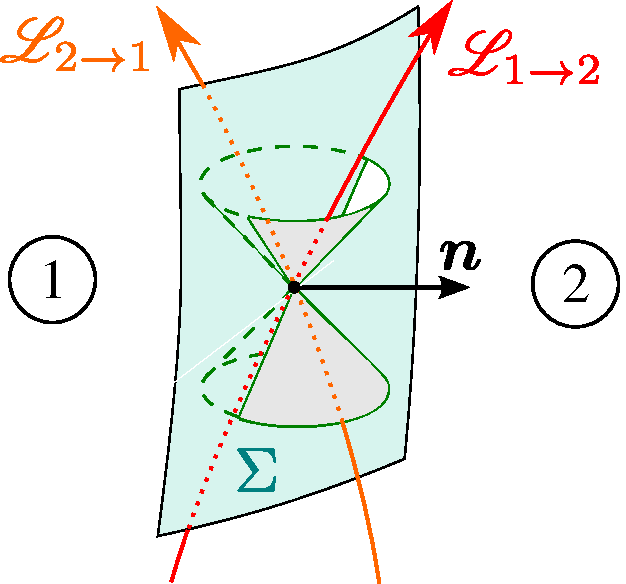
\includegraphics[width=0.4\textwidth]{def_timelike_2way.pdf}}
\caption[]{\label{f:def:timelike_2way} \footnotesize
A timelike hypersurface is a two-way membrane: $\Li_{1\rightarrow 2}$ is
a timelike worldline from Region~1 to Region~2, while $\Li_{2\rightarrow 1}$ is
a timelike worldline from Region~2 to Region~1.}
\end{figure}

\begin{figure}
\centerline{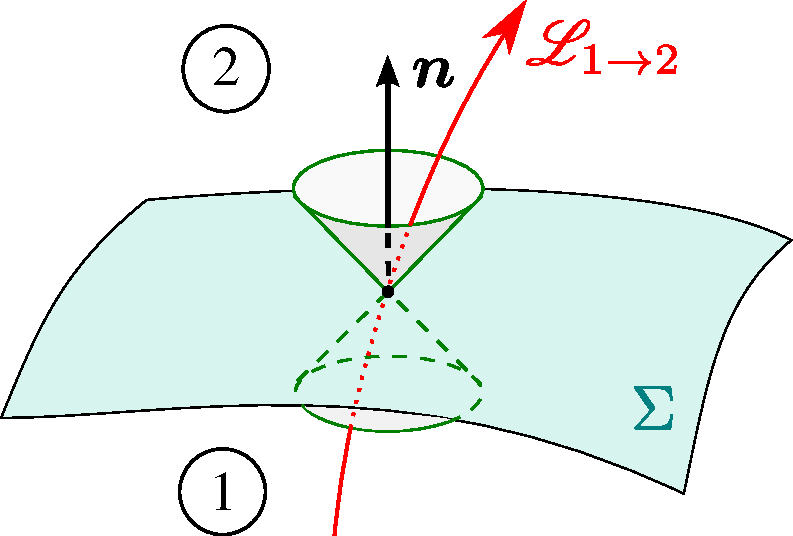
\includegraphics[width=0.5\textwidth]{def_spacelike_1way.pdf}}
\caption[]{\label{f:def:spacelike_1way} \footnotesize
A spacelike hypersurface is a one-way membrane: $\Li_{2\rightarrow 1}$ is
a timelike worldline from Region~2 to Region~1, while there is no timelike or null
worldline from Region~1 to Region~2.}
\end{figure}

\begin{figure}
\centerline{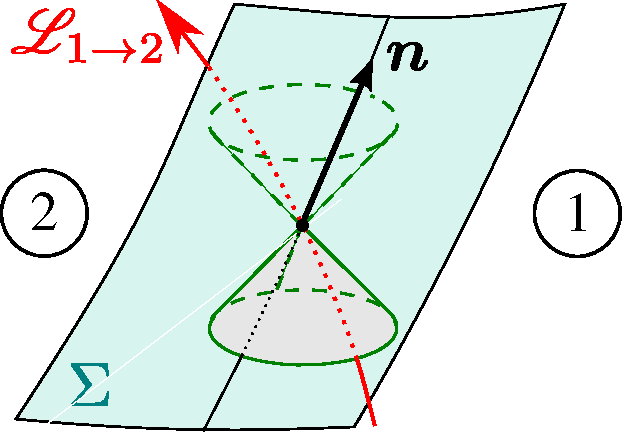
\includegraphics[width=0.5\textwidth]{def_null_1way.pdf}}
\caption[]{\label{f:def:null_1way} \footnotesize
A null hypersurface is a one-way membrane: $\Li_{2\rightarrow 1}$ is
a timelike worldline from Region~2 to Region~1, while there is no timelike or null
worldline from Region~1 to Region~2.}
\end{figure}

A timelike hypersurface is a two-way membrane: if it divides (locally)
spacetime in two regions, 1 and 2 say, and a future-directed timelike or null
worldline can cross it from Region~1 to Region~2, or from Region~2 to Region~1
(see Fig.~\ref{f:def:timelike_2way}). On the contrary,
a spacelike hypersurface is a one-way membrane: a future-directed timelike or null
worldline, which is constrained to move inside the light cones,
can cross it only from Region~2 to Region~1, say (see Fig.~\ref{f:def:spacelike_1way}).
A null hypersurface is also a one-way membrane (see Fig.~\ref{f:def:null_1way}).
At most, a null worldline that is not going from Region~2 to Region~1 must
stay on the hypersurface; an example of such null worldline is
the one depicted in Fig.~\ref{f:def:null_1way} as the thin black line tangent to the normal $\w{n}$.

The limit case between two-way membranes (timelike hypersurfaces)
and one-way ones being null hypersurfaces, it is quite natural to select the
latter ones for the black hole boundary, rather than spacelike hypersurfaces.
This choice will be fully justified in Chap.~\ref{s:glo}, where we shall see
that the precise definition of a black hole implies that its boundary
(the event horizon\index{event!horizon}\index{horizon!event --})
is a null hypersurface as soon as it is smooth (Property~4 in Sec.~\ref{s:glo:properties_H}).
Note however that in Chap.~\ref{s:loc}, we shall see that spacelike hypersurfaces,
called \emph{dynamical
horizons}\index{dynamical!horizon}\index{horizon!dynamical --}, are involved
in quasi-local approaches to black holes.

%%%%%%%%%%%%%%%%%%%%%%%%%%%%%%%%%%%%%%%%%%%%%%%%%%%%%%%%%%%%%%%%%%%%%%%%%%%%%%%%

\section{Geometry of null hypersurfaces} \label{s:def:geom_null_hypsurf}

Having decided that the black hole event horizon must be a null hypersurface,
let us examine the geometrical properties of such hypersurfaces. We shall
denote the hypersurface under study by $\Hor$, for \emph{horizon}, but the results of this section
will be valid for any null hypersurface.

\subsection{Hypersurfaces as level sets}

As any hypersurface, $\Hor$ can be locally considered as a level set\index{level set}:
around any point of $\Hor$, there exists an open subset $\mathscr{U}$
of $\M$ (possibly  $\mathscr{U} = \M$) and
a smooth scalar field $u:\ \mathscr{U} \rightarrow \R$ such that
\be \label{e:def:Hor_u_zero}
    \forall p \in \mathscr{U},\quad p\in \Hor \iff u(p) = 0 .
\ee
and
\be \label{e:def:du_not_zero}
    \wnab u \not = 0 \quad \mbox{on}\ \Hor .
\ee
Condition (\ref{e:def:du_not_zero}) ensures that $\Hor$ is a regular
hypersurface (an \emph{embedded} submanifold, in mathematical terms); without it, $\Hor$ may be
self-intersecting.

\begin{figure}
\centerline{\includegraphics[width=0.6\textwidth]{def_null_hplane.pdf}}
\caption[]{\label{f:def:null_hplane} \footnotesize
Null hyperplane $\Hor$ of equation $t-x=0$ in Minkowski spacetime.
The dimension along $z$ has been suppressed, so that $\Hor$ is pictured as a
2-plane.}
\end{figure}


\begin{example}[null hyperplane] \label{x:def:null_hyp}
A very simple example of null hypersurface is a null hyperplane of
the 4-dimensional Minkowski spacetime. The \defin{Minkowski spacetime}\index{Minkowski!spacetime} is defined by $\M=\mathbb{R}^4$ with $\w{g}$ being a \emph{flat} Lorentzian
metric. Natural coordinates are \defin{Minkowskian coordinates}\index{Minkowskian coordinates} $(t,x,y,z)$,
i.e. coordinates with
respect to which the metric components are $g_{\alpha\beta} = \mathrm{diag}(-1,1,1,1)$. The scalar field
\be \label{e:def:null_plane_u}
    u(t,x,y,z) = t - x
\ee
defines then a null hyperplane $\Hor$ by $u=0$ (cf. Fig.~\ref{f:def:null_hplane}).
\end{example}

\begin{example}[light cone] \label{x:def:light_cone}
Another simple example of null hypersurface, still in the 4-dimensional Minkowski spacetime,
is the future sheet $\Hor$ of a light cone\index{light!cone}\index{cone!light --}, also
called \defin{future light cone}\index{future!light cone}. Note that we have
to take out the cone apex from $\Hor$, in order to have a regular hypersurface.
In the  Minkowskian coordinates $(t,x,y,z)$, the choice of the
``retarded time''\index{retarded!time}
\be \label{e:def:light_cone_u}
    u(t,x,y,z) = t - \sqrt{x^2+y^2+z^2}
\ee
defines a future light cone $\Hor$ by $u=0$ and $t>0$ (cf.
Fig.~\ref{f:def:future_light_cone}).
\end{example}

\begin{figure}
\centerline{\includegraphics[width=0.6\textwidth]{def_future_light_cone.pdf}}
\caption[]{\label{f:def:future_light_cone} \footnotesize
Future sheet $\Hor$ of the light cone of equation $t-\sqrt{x^2+y^2+z^2}=0$ in Minkowski spacetime.
The dimension along $z$ has been suppressed, so that $\Hor$ looks 2-dimensional,
whereas it is actually 3-dimensional.}
\end{figure}


\begin{example}[Schwarzschild horizon] \label{x:def:Schw_hor}
Let us consider the 4-dimensional spacetime $(\M,\w{g})$ with $\M$ diffeomorphic
to $\mathbb{R}^4$ and equipped with a coordinate system $(x^\alpha)=(t,r,\th,\ph)$
($t\in \mathbb{R}$, $r\in(0,+\infty)$, $\th\in(0,\pi)$
and $\ph\in(0,2\pi)$) such that the metric tensor takes the
form\footnote{Formula (\ref{e:def:Schw_metric}) follows the notation
introduced in Eq.~(\ref{e:fra:g_components_dx}); see Sec.~\ref{s:bas:metric}
in Appendix~\ref{s:bas} for an extended discussion, in particular Eq.~(\ref{e:bas:sym_tensor_prod}).
When reading the metric components $(g_{\alpha\beta})$ from (\ref{e:def:Schw_metric}), keep in mind that
cross terms involve a factor $2$: the $4m/r$ coefficient of $\dd t \, \dd r$ implies
that $g_{tr} = 2m/r$.}
\be \label{e:def:Schw_metric}
    \w{g} = - \left( 1 - \frac{2 m}{r} \right) \dd t^2
        + \frac{4m}{r} \, \dd t \, \dd r
        + \left( 1 + \frac{2 m}{r} \right) \dd r^2
        + r^2\dd\th^2 + r^2\sin^2\th \, \dd\ph^2 ,
\ee
where $m$ is a positive constant. We shall see in Chap.~\ref{s:sch} that
$(\M,\w{g})$ is actually a part of Schwarzschild spacetime, described in
coordinates different from the standard Schwarzschild-Droste ones,  $(\bar t, r, \th, \ph)$
say, the link between the two being
$t = {\bar t} + 2m\ln|r/(2m)-1|$. The present coordinates are called the
\defin{ingoing Eddington-Finkelstein coordinates}\index{Eddington-Finkelstein!coordinates}
and have the advantage over the standard ones to be regular on the event horizon,
which is located at $r=2m$. Indeed, the metric components (\ref{e:def:Schw_metric})
remain finite when $r\rightarrow 2m$, as those of the inverse metric, which are
\be \label{e:def:Schw_metric_inv}
    g^{\alpha\beta} = \left(
    \begin{array}{cccc}
    - \left( 1 + \frac{2m}{r} \right) & \frac{2m}{r} & 0 & 0 \\
    \frac{2m}{r} & 1 - \frac{2m}{r} & 0 & 0 \\
    0 & 0 & \frac{1}{r^2} & 0 \\
    0 & 0 & 0 & \frac{1}{r^2\sin^2\th}
    \end{array} \right) .
\ee
Let us consider the scalar field defined on $\M$ by
\be \label{e:def:Schw_u}
    u(t,r,\th,\ph) = \left( 1 - \frac{r}{2m} \right)
            \exp\left(\frac{r-t}{4m}\right) .
\ee
It is then clear that the hypersurface $u=0$ is the
3-dimensional ``cylinder'' $\Hor$ of equation
$r=2m$ (cf. Fig.~\ref{f:def:Schwarz_horizon}). We shall see below\footnote{This should be obvious to the experienced
reader, since a normal 1-form to $\Hor$ is $\dd r$ and
from Eq.~(\ref{e:def:Schw_metric_inv}), $g^{\mu\nu} \partial_\mu r \, \partial_\nu r = g^{rr}=0$ on $\Hor$.} that $\Hor$ is indeed a null hypersurface.
\end{example}

\begin{figure}
\centerline{\includegraphics[width=0.5\textwidth]{def_Schwarz_horizon.pdf}}
\caption[]{\label{f:def:Schwarz_horizon} \footnotesize
Schwarzschild horizon $\Hor$ introduced in Example~\ref{x:def:Schw_hor};
The figure is drawn for $\th=\pi/2$ and is based on coordinates $(t,x,y)$
related to the ingoing Eddington-Finkelstein coordinates $(t,r,\th,\ph)$
by $x=r\cos\ph$ and $y=r\sin\ph$.}
\end{figure}



\subsection{Null normals} \label{s:def:null_normal}

Let $\wl$ be a vector field normal to $\Hor$. Since $\Hor$ is a null hypersurface,
$\wl$ is a null vector:
\be \label{e:def:wl_null}
    \wl\cdot\wl = 0 .
\ee
Moreover, we choose $\wl$ to be future-directed (cf. Sec.~\ref{s:fra:time_orientation}).

\begin{remark}
As a consequence of (\ref{e:def:wl_null}), there is no natural normalization
of $\wl$, contrary to the case of timelike or spacelike hypersurfaces,
where one can always choose the normal to be a unit vector
(scalar square equal to $1$ or $-1$). It follows that there is no unique choice
of $\wl$. At this stage, any rescaling $\wl \mapsto \wl' =  \alpha \wl$, with
$\alpha$ some strictly positive (to preserve the future orientation of $\wl$)
scalar field on $\Hor$,
yields a normal vector field $\wl'$ as valid as $\wl$.
\end{remark}
The null normal vector field $\wl$ is a priori defined on $\Hor$
only and not at points $p\not\in\Hor$.
However, it is worth to consider $\wl$ as a vector field
not confined to $\Hor$ but defined
in some open subset of $\M$ around $\Hor$.
In particular this would permit to define the spacetime covariant
derivative $\w{\nabla}\wl$, which is not possible if the
support of $\wl$ is restricted to $\Hor$.
Following Carter \cite{Carte97}, a simple way to achieve
this is to consider not only a single null hypersurface $\Hor$,
but a foliation of $\M$ (in the vicinity
of $\Hor$) by a family of null hypersurfaces, such that $\Hor$ is an
element of this family.
Without any loss of generality,
we may select the value of the scalar field $u$ defining $\Hor$ to label these hypersurfaces and
denote the family by $(\Hor_u)$. The null hypersurface $\Hor$
is then nothing but the element $\Hor = \Hor_{u=0}$ of this family
[Eq.~(\ref{e:def:Hor_u_zero})].
The vector field $\wl$ can then be viewed as being defined in the part of $\M$
foliated by $(\Hor_u)$, such that at each point in this region, $\wl$
is null and normal to $\Hor_u$ for some value of $u$.

\begin{figure}
\centerline{\includegraphics[height=0.4\textheight]{def_Schwarz_Hu.pdf}}
\caption[]{\label{f:def:Schwarz_Hu} \footnotesize
Hypersurfaces $\Hor_u$ defined by $u=\mathrm{const}$ for the example
of the Schwarzschild horizon (Example~\ref{x:def:Schw_hor}).}
\end{figure}



\begin{example}
The scalar field $u$ introduced in Example~\ref{x:def:null_hyp}
(null hyperplane) does define a family of null hypersurfaces
$(\Hor_u)$. A counter-example would be $u(t,x,y,z)=(t-x)(1+x^2)$, since
$u=a$ does not define a null hypersurface except for $a=0$.
Similarly, the scalar fields $u$ of
Example~\ref{x:def:light_cone} (light cone)
and Example~\ref{x:def:Schw_hor} (Schwarzschild horizon)
do define a family of null
hypersurfaces $(\Hor_u)$.
In the latter example, this would not have been the
case for the simpler choice $u(t,r,\th,\ph)  = r - 2m$.
Some of these null hypersurfaces are represented in Fig.~\ref{f:def:Schwarz_Hu}
\end{example}

Obviously the family $(\Hor_u)$ is non-unique but all geometrical
quantities that we shall introduce hereafter do not depend upon the choice
of the foliation $\Hor_u$ once they are evaluated at $\Hor$.

Since $\Hor$ is a hypersurface where $u$ is constant [Eq.~(\ref{e:def:Hor_u_zero})],
we have, by definition,
\bea
    \forall \w{v}\in T_p\M,\quad \w{v} \mbox{\ tangent to\ }\Hor & \iff  &
    \wnab_{\w{v}}\,  u = 0 \nonumber \\
    & \iff  & \langle \wnab u , \w{v} \rangle = 0 \nonumber \\
    & \iff & \vw{\nabla} u \cdot \w{v} = 0 ,   \label{e:def:nab_u_normal}
\eea
where $\vw{\nabla} u$ is the gradient vector field of the scalar field $u$,
i.e. the vector field given in index-notation by (cf. Sec.~\ref{s:bas:metric_dual})
\be \label{e:def:nab_up_u}
    \nabla^\alpha u = g^{\alpha\mu} \nabla_{\mu} u = g^{\alpha\mu} \der{u}{x^\mu} .
\ee
Property (\ref{e:def:nab_u_normal}) means that $\vw{\nabla} u$ is
a normal vector field to $\Hor$. By uniqueness of the normal direction to a hypersurface, it
must then be collinear to $\wl$. Therefore, there must exist some scalar
field $\rho$ such that
\be \label{e:def:wl_rho_u}
    \encadre{\wl = - \mathrm{e}^\rho \, \vw{\nabla} u } .
\ee
We have chosen the
coefficient linking $\wl$ and $\vw{\nabla} u $ to be strictly negative,
i.e. under the form of minus an exponential. This is always possible by a suitable
choice of the scalar field $u$. The minus sign ensures that in the case
of $u$ increasing toward the future, $\wl$ is future-directed,
as the following example shows:

\begin{example}[null hyperplane] \label{x:def:null_hyp2}
We deduce from the
expression (\ref{e:def:null_plane_u}) chosen for $u$ in Example~\ref{x:def:null_hyp} that
\[
    \wnab u = \dd t - \dd x .
\]
The gradient vector field obtained by metric duality is
$\vw{\nabla} u = - \wpar_t - \wpar_x$. Choosing for simplicity $\rho=0$,
we get from formula~(\ref{e:def:wl_rho_u})
\be \label{e:def:wl_null_hyperplane}
    \wl =  \wpar_t + \wpar_x .
\ee
The vector field $\wl$ is depicted in Fig.~\ref{f:def:null_hplane}.
\end{example}

\begin{example}[light cone] \label{x:def:light_cone2}
Regarding Example~\ref{x:def:light_cone}, we have,
given expression (\ref{e:def:light_cone_u}) for $u$,
\[
    \wnab u = \dd t - \frac{x}{r} \dd x - \frac{y}{r} \dd y - \frac{z}{r} \dd z,
    \quad\mbox{with}\quad r:=\sqrt{x^2+y^2+z^2}.
\]
Choosing for simplicity $\rho=0$ in (\ref{e:def:wl_rho_u}), we get the
normal
\be \label{e:def:wl_light_cone}
    \wl = \wpar_t + \frac{x}{r} \wpar_x + \frac{y}{r} \wpar_y + \frac{z}{r} \wpar_z .
\ee
The vector field $\wl$ is depicted in Fig.~\ref{f:def:future_light_cone}.
\end{example}

\begin{example}[Schwarzschild horizon] \label{x:def:Schw_hor2}
We deduce from the expression (\ref{e:def:Schw_u}) chosen for $u$ in
Example~\ref{x:def:Schw_hor} that
\[
    \wnab u = \frac{1}{4 m} \mathrm{e}^{(r-t)/(4m)} \left[ - \left(1-\frac{r}{2m}  \right)
        \, \dd t
        - \left(1 + \frac{r}{2m}\right) \, \dd r \right] .
\]
The corresponding gradient vector field,
is computed from (\ref{e:def:nab_up_u}) via expression
(\ref{e:def:Schw_metric_inv}) for $g^{\alpha\mu}$:
\[
    \vw{\nabla} u = \frac{1}{4 m} \mathrm{e}^{(r-t)/(4m)} \left[
    - \left(1+ \frac{r}{2m} \right) \wpar_t
    + \left(1 - \frac{r}{2m} \right) \wpar_r \right] .
\]
This time, we do not chose $\rho=0$ but rather select $\rho$ so that
$\el^t = 1$:
\be \label{e:def:rho_Schw_hor}
    \mathrm{e}^\rho =  - \frac{1}{\nabla^t u} \iff
    \rho = \frac{t-r}{4m} - \ln \left( 1 + \frac{r}{2m} \right) + \ln (4 m).
\ee
Equation~(\ref{e:def:wl_rho_u}) leads then to
\be \label{e:def:wl_Schw_hor}
    \wl = \wpar_t +  \frac{r-2m}{r+2m} \,  \wpar_r .
\ee
Given the metric (\ref{e:def:Schw_metric}), we check that $\w{g}(\wl, \wl)=0$.
Since $\wl\not=0$, this proves that all hypersurfaces $\Hor_u$, and in particular $\Hor$,
are null.
The vector field $\wl$ is depicted on $\Hor$ in Fig.~\ref{f:def:Schwarz_horizon}
and in all space in Fig.~\ref{f:def:Schw_hor_lk}.
\end{example}

\subsection{Null geodesic generators} \label{s:def:null_geod_gen}

\subsubsection{Frobenius identity} \label{s:def:Frobenius}

Let us take the metric dual of relation (\ref{e:def:wl_rho_u}): it writes
$\uu{\el} = - \mathrm{e}^\rho \, \wnab u$, or, in index notation,
\be
    \el_\alpha = - \mathrm{e}^\rho \, \nabla_\alpha u .
\ee
Taking the covariant derivative, we get
\[
    \nabla_\alpha \el_\beta = - \mathrm{e}^\rho \nabla_\alpha \rho \nabla_\beta u
                -   \mathrm{e}^\rho  \nabla_\alpha \nabla_\beta u
                 = \nabla_\alpha \rho \, \el_\beta - \mathrm{e}^\rho  \nabla_\alpha \nabla_\beta u
\]
Antisymmetrizing and using the torsion-free property of $\wnab$ (i.e.
$\nabla_\alpha \nabla_\beta u - \nabla_\beta \nabla_\alpha u = 0$, cf.
Eq.~(\ref{e:bas:torsion-free}) in Appendix~\ref{s:bas}), we get
\be \label{e:def:ext_der_wl_comp}
  \nabla_\alpha \el_\beta - \nabla_\beta \el_\alpha =
  \nabla_\alpha \rho \, \el_\beta -  \nabla_\beta \rho \, \el_\alpha  .
\ee
In the left-hand side there appears the exterior derivative of
the 1-form $\uu{\el}$ (cf. Sec.~\ref{s:bas:ext_deriv} in Appendix~\ref{s:bas}),
while one recognize in the right-hand side the exterior product of
the two 1-forms $\dd\rho$ and $\uu{\el}$. Hence we may rewrite (\ref{e:def:ext_der_wl_comp})
as
\be
    \encadre{ \dd \uu{\el} = \dd\rho \wedge \uu{\el} } .
\ee
This reflects the \defin{Frobenius theorem}\index{Frobenius!theorem}
in its dual formulation (see e.g.
Theorem B.3.2 in Wald's textbook \cite{Wald84} or Theorem C.2 in
Straumann's textbook \cite{Strau13}): the exterior derivative of
the 1-form $\uu{\el}$ is the exterior product of $\uu{\el}$ itself with some
1-form ($\dd\rho$ in the present case) if, and only if,
$\uu{\el}$ defines hyperplanes that are integrable in some hypersurface ($\Hor$ in the present case).

\subsubsection{Geodesic generators} \label{s:def:geod_gener}

Let us contract the Frobenius identity (\ref{e:def:ext_der_wl_comp}) with $\wl$:
\be \label{e:def:l_contract_Frob}
    \el^\mu \nabla_\mu \el_\alpha - \el^\mu \nabla_\alpha \el_\mu
        = \el^\mu \nabla_\mu \rho \, \el_\alpha
        - \underbrace{\el^\mu \el_\mu}_{0} \nabla_\alpha \rho .
\ee
Now, since $\wl$ is a null vector,
\[
    \el^\mu \nabla_\alpha \el_\mu = \nabla_\alpha (\underbrace{\el^\mu \el_\mu}_{0})
        - \el_\mu \nabla_\alpha \el^\mu ,
\]
from which we get
\be \label{e:def:el_nab_el_zero}
    \el^\mu \nabla_\alpha \el_\mu = 0 .
\ee
Hence (\ref{e:def:l_contract_Frob}) reduces to
\be \label{e:def:wl_geod_kappa_dual}
    \el^\mu \nabla_\mu \el_\alpha  = \kappa \, \el_\alpha ,
\ee
with
\be \label{e:def:def_kappa}
    \kappa := \el^\mu \nabla_\mu \rho = \wnab_{\wl}\,  \rho .
\ee
The metric dual of (\ref{e:def:wl_geod_kappa_dual}) is
\be \label{e:def:wl_geod_kappa}
    \encadre{ \wnab_{\wl}\, \wl = \kappa \, \wl } .
\ee
This equation implies that the field lines of $\wl$ are geodesics
(cf. Appendix~\ref{s:geo}).
To demonstrate this, we note that a rescaling
\be \label{e:def:wl_rescale}
    \wl \mapsto \wl' =  \alpha \wl
\ee
with $\alpha$ a positive scalar field can be performed to yield
a \defin{geodesic vector field}\index{geodesic!vector field} $\wl'$, i.e.
a vector field that obeys\footnote{A vector field that obeys the weaker condition
(\ref{e:def:wl_geod_kappa}), with $\kappa$ possibly different from zero, is called
a \defin{pregeodesic vector field}\index{pregeodesic!vector field}, cf.
Sec.~\ref{s:geo:gener_param} in Appendix~\ref{s:geo}.} Eq.~(\ref{e:geo:geod_eq_v}):
\be \label{e:def:wlp_geod}
    \wnab_{\wl'}\, \wl' = 0 .
\ee
\begin{proof}
Equations~(\ref{e:def:wl_rescale}) and
(\ref{e:def:wl_geod_kappa}) imply
\be \label{e:def:nab_lp_lp}
    \wnab_{\wl'}\, \wl' = \alpha\left(
        \wnab_{\wl}\, \alpha + \kappa \alpha \right) \wl .
\ee
Hence, since $\alpha>0$,
\[
    \wnab_{\wl'}\, \wl' = 0  \iff  \wnab_{\wl}\, \ln \alpha = -\kappa .
\]
Therefore, it suffices to solve $\wnab_{\wl}\, \ln \alpha = -\kappa$, which
is a first-order ordinary differential equation along each field line of $\wl$,
to ensure that $\wl'$ is a geodesic vector field.
\end{proof}
Because of (\ref{e:def:wlp_geod}),
the field lines of $\wl'$ are  null geodesics and $\wl'$ is the tangent
vector to them associated with some affine parameter $\lambda$.
On the other side, if $\kappa\not=0$, $\wl$ is not a geodesic vector field
and therefore cannot be associated with some affine parameter. For this
reason the quantity $\kappa$ is called the
\defin{non-affinity coefficient}\index{non-affinity coefficient} of
the null normal $\wl$ (cf. Sec.~\ref{s:geo:gener_param} in Appendix~\ref{s:geo}).

Since $\wl$ is collinear to $\wl'$, it obviously shares the same field lines,
which have just been shown to be null geodesics. These field lines are called the
\defin{null geodesic generators}\index{null!geodesic!generator}\index{generator!of a null hypersurface} of the hypersurface $\Hor$.

Hence, we have shown that
\begin{greybox}
Any null hypersurface $\Hor$ is ruled by a family of null geodesics, called the
\emph{generators of $\Hor$}, and each vector field $\wl$ normal to $\Hor$ is
tangent to these null geodesics.
\end{greybox}

\begin{remark}
\label{r:def:null_curves}
The above result is not trivial: while it is obvious that the field lines of the normal
vector field $\wl$ are null curves that are tangent to $\Hor$, the reader must
keep in mind that not all null curves are null geodesics. For instance, in
Minkowski spacetime, the helix defined in terms of
some Minkowskian coordinates $(x^\alpha)=(t,x,y,z)$ by the parametric equation
$x^\alpha(\lambda) = (\lambda, \cos\lambda, \sin\lambda, 0)$ is a null curve, i.e.
it has
a null tangent vector at each point, but it is not a null geodesic: in Minkowski
spacetime, all null geodesics are straight lines.
\end{remark}

As a by-product of (\ref{e:def:nab_lp_lp}), we get the behaviour of the
non-affinity coefficient under a rescaling of the null normal:
\be \label{e:def:rescale_kappa}
    \wl' = \alpha \wl \ \Longrightarrow \ \kappa' = \alpha \kappa + \wnab_{\wl} \alpha .
\ee

\begin{example}[null hyperplane] \label{x:def:null_hyp3}
It is clear on expression (\ref{e:def:wl_null_hyperplane}) for $\wl$ that
the covariant derivative
$\wnab \wl$ vanishes identically. In particular $\wnab_{\wl} \wl = 0$.
Equation~(\ref{e:def:wl_geod_kappa}) then implies
\be \label{e:def:kappa_0_nullhyp}
    \kappa = 0 ,
\ee
which is in agreement with Eq.~(\ref{e:def:def_kappa}) and the choice $\rho=0$
performed in Example~\ref{x:def:null_hyp2}. The null geodesic generators of $\Hor$ are the
straight lines defined by $t=x$, $y=y_0$ and $z=z_0$ for some constants
$(y_0,z_0)\in \mathbb{R}^2$.
They are depicted as green lines in Fig.~\ref{f:def:null_hplane}.
 Either $t$ or $x$ can be chosen as affine
parameters of these generators.
\end{example}

\begin{example}[light cone] \label{x:def:light_cone3}
From expression (\ref{e:def:wl_light_cone})
for $\wl$ and the fact that
$\nabla_\beta \el^\alpha = \partial_\beta \el^\alpha$
in the Minkowskian coordinates $(t,x,y,z)$, we get
\be \label{e:def:nab_l_light_cone}
    \nabla_\beta \el^\alpha = \left(
    \begin{array}{cccc}
    0 & 0 & 0 & 0 \\
    0 & \frac{y^2+z^2}{r^3} & - \frac{xy}{r^3} & - \frac{xz}{r^3} \\
    0 & - \frac{xy}{r^3} & \frac{x^2+z^2}{r^3} & - \frac{yz}{r^3} \\
    0 & - \frac{xz}{r^3} & - \frac{yz}{r^3} & \frac{x^2+y^2}{r^3}
    \end{array} \right)
    \qquad {(\alpha = \mbox{row index}; \atop \beta = \mbox{column index}).}
\ee
We obtain then $\el^\mu \nabla_\mu \el^\alpha = 0$.
From Eq.~(\ref{e:def:wl_geod_kappa}), we conclude that
\[
    \kappa = 0 ,
\]
which is in agreement with Eq.~(\ref{e:def:def_kappa}) and the choice $\rho=0$
performed in Example~\ref{x:def:light_cone2}. The null geodesic generators of $\Hor$
are the half-lines defined by $x=a t$, $y=b t$, $z = \sqrt{1-a^2-b^2} t$, with
$t>0$ and $(a,b)\in\mathbb{R}^2$ such that $a^2+b^2 \leq 1$.
They are depicted as green lines in Fig.~\ref{f:def:future_light_cone}.
Since from (\ref{e:def:wl_light_cone}) $\wnab_{\wl} t = 1$
and $\kappa=0$, $\lambda=t$ is an affine parameter along these null geodesic generators.
\end{example}

\begin{example}[Schwarzschild horizon] \label{x:def:Schw_hor3}
The covariant derivative of the vector field $\wl$ as given by (\ref{e:def:wl_Schw_hor})
is (cf. Sec.~\ref{s:sam:Schwarz_hor} for the computation)
\be \label{e:def:nab_l_Schw_hor}
    \nabla_\beta \el^\alpha = \left(
    \begin{array}{cccc}
    \frac{m}{r^2} & \frac{m}{r^2} \frac{3r+2m}{r+2m} & 0 & 0 \\[1ex]
    \frac{m}{r^2}\frac{r-2m}{r+2m} & \frac{m}{r^2}\frac{3r^2-4m(r+m)}{(r+2m)^2} & 0 & 0 \\[1ex]
    0 & 0 & \frac{r-2m}{r(r+2m)} & 0 \\
    0 & 0 & 0 & \frac{r-2m}{r(r+2m)}
    \end{array} \right)
    \qquad {(\alpha = \mbox{row index}; \atop \beta = \mbox{column index}).}
\ee
Contracting with $\wl^\beta$, we obtain
\[
    \wnab_{\wl} \wl = \frac{4m}{(r+2m)^2} \wpar_t
        +  \frac{4m(r-2m)}{(r+2m)^3} \,  \wpar_r = \frac{4m}{(r+2m)^2}  \, \wl .
\]
Hence, for any $\Hor_u$, $\kappa=4m/(r+2m)^2$. On $\Hor$ ($r=2m$), we get
\be \label{e:def:kappa_Schw_hor}
   \kappa = \frac{1}{4m} .
\ee
This value agrees with $\kappa = \wnab_{\wl}\rho$ [Eq.~(\ref{e:def:def_kappa})] and the
choice (\ref{e:def:rho_Schw_hor}) made for $\rho$. Contrary to Examples~\ref{x:def:null_hyp3}
and \ref{x:def:light_cone3}, $\kappa$ does not vanish; hence $t$, which is
a parameter of the null geodesic generators associated with $\wl$ (since $\wnab_{\wl} t = 1$
by virtue of (\ref{e:def:wl_Schw_hor})),
is \emph{not} an affine parameter. The null geodesic generators are depicted
as vertical green lines in Fig.~\ref{f:def:Schwarz_horizon}.
\end{example}

\subsection{Cross-sections} \label{s:def:spacelike_sections}

Let us now focus on the first aspect of the black hole definition given
in Sec.~\ref{s:def:first_defin}: \emph{localization}.
This feature is crucial to distinguish a black hole boundary from other kinds
of null hypersurfaces. For instance the interior of a future null cone
in Minkowski spacetime is a region from which no particle may escape,
but since the null cone is expanding, particles can travel arbitrary far from
the center. Therefore, a null cone does not define a black hole.
A key parameter is hence the \emph{expansion} of null hypersurfaces, which we shall
discuss in the next section, after having introduced cross-sections.

\begin{figure}
\centerline{\includegraphics[width=0.5\textwidth]{def_cross_sections.pdf}}
\caption[]{\label{f:def:hor_cylinder} \footnotesize
The null hypersurface $\Hor$ and two cross-sections $\Sp$ and $\Sp'$.
The green curves represent some null geodesic generators, with the null normal
$\wl$ tangent to them.}
\end{figure}

In the remaining of this chapter, we assume that the spacetime dimension $n$
obeys $n\geq 3$. We define then a \defin{cross-section}\index{cross-section}
of the null hypersurface $\Hor$
as a submanifold $\Sp$ of $\Hor$ of codimension 2 (i.e. $\dim \Sp=n-2$),
such that (i) the null normal $\wl$ is nowhere tangent to $\Sp$ and (ii)
each null geodesic generator of $\Hor$ intersects $\Sp$ once, and only once.

\begin{notation}
Indices relative to a cross-section will range from $2$ to $n-1$ and
will be denoted by a Latin letter from the beginning of the alphabet: $a$, $b$, etc.
\end{notation}

To encompass the idea that an event horizon delimitates some
region of spacetime, we shall assume that the cross-sections
are \defin{closed manifolds}\index{closed!manifold}, i.e.
are compact without boundary. The simplest example is the sphere,
more precisely the $(n-2)$-dimensional sphere $\mathbb{S}^{n-2}$, where $n$
is the spacetime dimension. It is the one relevant for standard 4-dimensional
black holes. But at this stage, we shall allow for other
closed-manifold topologies, like that of a torus.

Given the definition of a cross-section $\Sp$,
the topology of $\Hor$ is then that of a ``tube'' or ``cylinder''
(cf. Fig.~\ref{f:def:hor_cylinder}):
\be \label{e:def:H_topology}
    \Hor \simeq \R \times \Sp.
\ee
For the standard 4-dimensional black holes, this is
$\Hor \simeq \R \times \mathbb{S}^{2}$.

A first important property is
\begin{greybox}
Any cross-section $\Sp$ is spacelike,
i.e. all vectors tangent to $\Sp$ are spacelike.
\end{greybox}
\begin{proof}
The spacelike character of $\Sp$ follows from
\begin{greybox}
\textbf{Lemma (vectors tangent to a null hypersurface)}\\[1ex]
Every nonzero vector tangent to a null hypersurface is either spacelike or null.
Moreover, in the latter case, it is tangent to a null geodesic generator (i.e. it is normal
to the hypersurface).
\end{greybox}
\begin{proof}
Tangent vectors to a null hypersurface $\Hor$ are by definition
vectors $\w{v}$ such that $\w{g}(\wl,\w{v})=0$, where $\wl$ is the normal
to $\Hor$. Since $\wl$ is null, it follows then from Corollary~1
of Sec.~\ref{s:fra:time_orientation} that $\w{v}$ cannot be timelike.
Besides, if $\w{v}$ is null, Corollary~2 of Sec.~\ref{s:fra:time_orientation}
implies that it must be collinear to $\wl$.
\end{proof}
Let $p \in \Sp$ and $\w{v}\in T_p\M$ be a nonzero vector tangent to $\Sp$.
The above lemma implies that $\w{v}$ is either spacelike or tangent to the
null geodesic generator $\Li$ going through $p$, but then $\Li$ would be tangent to $\Sp$,
which is not allowed, given the definition of a cross-section. We conclude
that $\w{v}$ is necessarily spacelike, which proves that $\Sp$ is a spacelike
submanifold.
\end{proof}

\begin{example}[light cone] \label{x:def:light_cone4}
From now on, we abandon the null hyperplane considered in Examples~\ref{x:def:null_hyp},
\ref{x:def:null_hyp2} and \ref{x:def:null_hyp3}, since its topology is $\mathbb{R}^3$,
and therefore not of the type (\ref{e:def:H_topology}) with $\Sp$ compact.
On the other side, the future sheet $\Hor$ of the Minkowski-spacetime light cone considered in Examples~\ref{x:def:light_cone},
\ref{x:def:light_cone2} and \ref{x:def:light_cone3} does obey (\ref{e:def:H_topology}),
since we have excluded the cone apex from $\Hor$.
A natural choice of cross-section is a sphere defined by $t=t_0$ for some positive constant $t_0$:
\[
    \Sp = \left\{ p \in \Hor,\  t(p) = t_0 \right\} .
\]
That $\Sp$ is a 2-dimensional sphere in the hyperplane $t=t_0$ is clear on its equation in terms
of the Minkowskian coordinates $(t,x,y,z)$:
\[
\Sp: \quad t=t_0 \quad\mbox{and}\quad x^2+y^2+z^2 = t_0^2,
\]
which follows immediately from $u=0$
[cf. Eq.~(\ref{e:def:light_cone_u})]. Moreover, this equation shows that the
radius of the sphere is $t_0$.
\end{example}

\begin{example}[Schwarzschild horizon] \label{x:def:Schw_hor4}
The 3-dimensional cylinder $\Hor$ introduced in Example~\ref{x:def:Schw_hor}
has the topology (\ref{e:def:H_topology}), with $\Sp\simeq \mathbb{S}^2$
(cf. Fig.~\ref{f:def:Schwarz_horizon}).
Since it is defined
by $r=2m$ in terms of the ingoing Eddington-Finkelstein coordinates $(t,r,\th,\ph)$,
a natural coordinate system on $\Hor$ is $x^A = (t,\th,\ph)$. Moreover, we
have seen that the coordinate $t$ is the (non-affine) parameter of the null
geodesics generating $\Hor$ associated with the null normal $\wl$.
As in Example~\ref{x:def:light_cone4}, a natural choice of cross-section is a
sphere defined by $t=t_0$ for some constant $t_0$:
\[
    \Sp = \left\{ p \in \Hor,\  t(p) = t_0 \right\} .
\]
The equation of $\Sp$ in terms of the coordinates $(t,r,\th,\ph)$ is then
\[
    \Sp: \quad t=t_0 \quad\mbox{and}\quad r = 2m .
\]
Note that $x^a=(\th,\ph)$ constitutes a coordinate system on $\Sp$.
\end{example}

\begin{example}[binary black hole]
Some cross-sections of the event horizon $\Hor$ in numerically
generated binary black hole spacetimes are displayed in Figs.~\ref{f:glo:EH_headon}
and \ref{f:glo:EH_binspir} of Chap.~\ref{s:glo}.
\end{example}

Let us denote by $\w{q}$ the
\defin{metric induced by $\w{g}$ on $\Sp$}\index{induced!metric}\index{metric!induced --},
i.e. the bilinear form defined at any point $p\in\Sp$ by
\be \label{e:def:def_q_S}
    \forall (\w{u},\w{v})\in T_p\Sp\times T_p\Sp, \quad
     \w{q}(\w{u},\w{v}) = \w{g}(\w{u},\w{v}) .
\ee
Saying that $\Sp$ is spacelike is equivalent to saying that $\w{q}$ is
positive definite, i.e.
\be
    \forall \w{v}\in T_p\Sp,\quad
    \w{q}(\w{v},\w{v}) \geq 0 \quad \mbox{and} \quad
    \w{q}(\w{v},\w{v}) = 0 \iff \w{v} = 0.
\ee
In other words, $(\Sp, \w{q})$ is a \defin{Riemannian manifold}\index{Riemannian!manifold} (cf Sec.~\ref{s:bas:signature} in Appendix~\ref{s:bas}).

\begin{example}[Schwarzschild horizon] \label{x:def:Schw_hor4a}
The metric induced by $\w{g}$ on the cross-section
$\Sp$ of the Schwarzschild horizon defined in Example~\ref{x:def:Schw_hor4} is readily obtained by
setting $t=\mathrm{const}=t_0$ and $r=\mathrm{const}=2m$ in Eq.~(\ref{e:def:Schw_metric}),
since  $x^a=(\th,\ph)$ is a coordinate system on $\Sp$:
\be \label{e:def:q_S_Schw_hor}
    \w{q} = 4m^2 \left( \dd\th^2 + \sin^2\th \, \dd\ph^2 \right) .
\ee
\end{example}

\begin{figure}
\centerline{\includegraphics[width=0.5\textwidth]{def_2surf_ortho_complement.pdf}}
\caption[]{\label{f:def:TS_ortho} \footnotesize
The tangent space $T_p\Sp$ to the cross-section $\Sp$ and its 2-dimensional
orthogonal complement
$T_p^\perp\Sp$. Only the dimensionality of the latter is respected in
the figure: $\Sp$ and $T_p\Sp$ are depicted as 1-dimensional
objects, while they are truly $(n-2)$-dimensional ones.}
\end{figure}

An important consequence of $\Sp$ being spacelike is that, at each point
$p\in \Sp$, the tangent space $T_p\Sp$ has an orthogonal complement
$T_p^\perp\Sp$,  which is a timelike plane such that
$T_p\M$ is the direct sum of $T_p\Sp$ and $T_p^\perp\Sp$ :
\be \label{e:def:TM_direct_sum}
   \encadre{ \forall p\in \Sp,\quad T_p\M = T_p\Sp \oplus T_p^\perp\Sp }.
\ee
That $T_p^\perp\Sp$ is timelike is necessary for the signature of $\w{g}$
to be $(-,+,\ldots,+)$. This can be seen by constructing an $\w{g}$-orthogonal
basis of $T_p\M$ by the Gram-Schmidt process, starting form a
$\w{q}$-orthogonal basis of $T_p\Sp$. Since $\dim T_p\Sp = n-2$, we have
$\dim T_p^\perp\Sp = 2$, i.e. $T_p^\perp\Sp$ is a timelike 2-plane.
In other words, the metric induced by $\w{g}$ on
$T_p^\perp\Sp$ is Lorentzian:
\be
    \mathrm{sign}\, \left.\w{g}\right|_{T_p^\perp\Sp} = (-,+) .
\ee
Since $\Sp\subset\Hor$, the null normal $\wl$ to $\Hor$ is orthogonal to any vector
tangent to $\Sp$, i.e. $\wl \in T_p^\perp\Sp$.
Now, as a timelike plane, $T_p^\perp\Sp$ has two independent null directions,
which can be seen as the two intersections of the null cone at $p$ with
the 2-plane $T_p^\perp\Sp$ (cf. Fig.~\ref{f:def:TS_ortho}).
Let us denote by $\w{k}$ a future-directed null vector in the null direction of $T_p^\perp\Sp$
that is not along $\wl$. By a proper rescaling $\w{k}\mapsto \alpha\w{k}$,
we may choose $\w{k}$ so that
\be \label{e:def:k_el_minus_one}
        \w{k}\cdot\wl = -1 .
\ee
Given $\wl$ and $\Sp$, the condition (\ref{e:def:k_el_minus_one})
determines the null vector $\w{k}$ uniquely.
Since $\wl$ and $\w{k}$ are non-collinear vectors of $T_p^\perp\Sp$ and
$\dim T_p^\perp\Sp = 2$, they constitute a basis of $T_p^\perp\Sp$:
\be \label{e:def:TSperp_Span_k_l}
    T_p^\perp\Sp = \mathrm{Span}\left( \wl, \w{k} \right) .
\ee

A priori, the bilinear form $\w{q}$ is defined only on $T_p\Sp$, via (\ref{e:def:def_q_S}).
However, thanks to the orthogonal decomposition (\ref{e:def:TM_direct_sum}),
we can extend it to all vectors of $T_p\M$ by requiring
\be \label{e:def:q_zero_TSperp}
    \forall \w{u}\in T_p^\perp\Sp,\ \forall\w{v}\in T_p\M, \quad \w{q}(\w{u}, \w{v}) = 0 .
\ee
Indeed, given a pair $(\w{u},\w{v})$ of vectors in $T_p\M$, the direct sum (\ref{e:def:TM_direct_sum})
implies that there are unique decompositions
\be \label{e:def:decomp_u_v}
  \w{u} = \w{u}^\parallel + \w{u}^\perp \quad\mbox{and}\quad
    \w{v} = \w{v}^\parallel + \w{v}^\perp,\quad\mbox{with}\quad
    \w{u}^\parallel,  \w{v}^\parallel \in T_p\Sp,\quad
    \w{u}^\perp, \w{v}^\perp  \in T_p^\perp\Sp .
\ee
Then, using the bilinearity of $\w{q}$ and property (\ref{e:def:q_zero_TSperp}),
we obtain
\be \label{e:def:q_all_vectors}
    \forall (\w{u},\w{v})\in T_p\M\times T_p\M, \quad
     \w{q}(\w{u},\w{v}) = \w{q}(\w{u}^\parallel,\w{v}^\parallel) .
\ee
Equation~(\ref{e:def:q_all_vectors}), along with (\ref{e:def:def_q_S}), can
be considered as the definition of $\w{q}$. An equivalent definition,
which provides an explicit expression of $\w{q}$, is
\be \label{e:def:q_g_k_l}
    \encadre{ \w{q} = \w{g} + \uu{\el}\otimes\uu{k} + \uu{k}\otimes\uu{\el} } ,
\ee
or, in index notation,
\be
   \encadre{ q_{\alpha\beta} = g_{\alpha\beta} + \el_\alpha k_\beta + k_\alpha \el_\beta }.
\ee
\begin{proof}
Let us show that (\ref{e:def:q_g_k_l}) implies
(\ref{e:def:q_all_vectors})-(\ref{e:def:def_q_S}).
Starting from (\ref{e:def:q_g_k_l}), we have for any pair of vectors $(\w{u},\w{v})$
in $T_p\M$,
\be \label{e:def:q_u_v_k_l}
    \w{q}(\w{u},\w{v}) = \w{u}\cdot\w{v} + (\wl\cdot\w{u})(\w{k}\cdot\w{v})
    + (\w{k}\cdot\w{u})(\wl\cdot\w{v}) .
\ee
Now, thanks to (\ref{e:def:TSperp_Span_k_l}), we may write the
orthogonal decompositions (\ref{e:def:decomp_u_v}) as
\[
    \w{u} = \w{u}^\parallel + u^0 \wl + u^1 \w{k} \quad\mbox{and}\quad
    \w{v} = \w{v}^\parallel + v^0 \wl + v^1 \w{k} .
\]
Using $\wl\cdot\wl=0$, $\w{k}\cdot\w{k}=0$ and $\wl\cdot\w{k}=-1$
[Eq.~(\ref{e:def:k_el_minus_one})], we have then
\bea
 & & \w{u}\cdot\w{v} = \w{u}^\parallel \cdot\w{v}^\parallel - u^0 v^1 - u^1 v^0 \nonumber \\
 & & \wl\cdot\w{u} = -u^1, \quad \w{k}\cdot\w{u} = -u^0, \quad
  \wl\cdot\w{v} = -v^1, \quad \w{k}\cdot\w{v} = -v^0 .  \nonumber
\eea
Hence (\ref{e:def:q_u_v_k_l}) results in
\[
    \w{q}(\w{u},\w{v}) = \w{u}^\parallel \cdot\w{v}^\parallel - u^0 v^1 - u^1 v^0
            + u^1 v^0 + u^0 v^1 = \w{u}^\parallel \cdot\w{v}^\parallel,
\]
which is nothing but (\ref{e:def:q_all_vectors}).
\end{proof}

\begin{example}[light cone] \label{x:def:light_cone5}
In continuation with Example~\ref{x:def:light_cone4}, the null
vector $\w{k}$ orthogonal to the sphere $\Sp$ and obeying $\w{k}\cdot\wl = -1$
is
\[
    \w{k} = \frac{1}{2} \wpar_t
        - \frac{x}{2r} \wpar_x - \frac{y}{2r} \wpar_y  - \frac{z}{2r} \wpar_z .
\]
Evaluating $\w{q}$ via (\ref{e:def:q_g_k_l}), given expression
(\ref{e:def:wl_light_cone}) for $\wl$, we get the following components
of $\w{q}$ with respect to the Minkowskian coordinates $x^\alpha=(t,x,y,z)$:
\[
    q_{\alpha\beta} = \left(
    \begin{array}{cccc}
    0 & 0 & 0 & 0 \\
    0 & \frac{y^2+z^2}{r^2} & - \frac{xy}{r^2} & - \frac{xz}{r^2} \\
    0 & - \frac{xy}{r^2} & \frac{x^2+z^2}{r^2} & - \frac{yz}{r^2} \\
    0 & - \frac{xz}{r^2} & - \frac{yz}{r^2} & \frac{x^2+y^2}{r^2}
    \end{array} \right) .
 \]
If we consider the spherical coordinates ${x'}^{\alpha}=(t,r,\th,\ph)$
deduced from the Minkowskian ones via the standard formulas:
\[
    \left\{ \begin{array}{l}
    x = r\sin\th\cos\ph \\
    y = r\sin\th\sin\ph \\
    z = r\cos\th
    \end{array} \right. ,
\]
the components of $\w{q}$ become instead
\be \label{e:def:q_light_cone_spher}
    q'_{\alpha\beta} = \left(
    \begin{array}{cccc}
    0 & 0 & 0 & 0 \\
    0 & 0 & 0 & 0 \\
    0 & 0 & r^2 & 0 \\
    0 & 0 & 0 & r^2\sin^2\th
    \end{array} \right) .
\ee
and we recognize in $q'_{ab} = \mathrm{diag}(r^2, r^2 \sin^2\th)$ the
standard metric on the 2-sphere of radius $r$.
\end{example}

\begin{figure}
\centerline{\includegraphics[width=0.6\textwidth]{def_plot_lk.pdf}}
\caption[]{\label{f:def:Schw_hor_lk} \footnotesize
Null vector fields $\wl$ (green) and $\w{k}$ (red) corresponding to
Example~\ref{x:def:Schw_hor5} (Schwarzschild horizon).
The plot is a 2-dimensional slice $\th=\mathrm{const}$ and $\ph=\mathrm{const}$
of the spacetime $\M$, with $t$ and $r$ labelled in units of $m$.
Note that
since $\w{k}$ diverges at $r=0$ [cf. Eq.~(\ref{e:def:k_Schw_hor})], it is not represented there.}
\end{figure}

\begin{example}[Schwarzschild horizon] \label{x:def:Schw_hor5}
For the Schwarzschild horizon case, we deduce from the metric (\ref{e:def:Schw_metric})
and the expression (\ref{e:def:wl_Schw_hor}) for $\wl$ that the null
vector $\w{k}$ orthogonal to the sphere $\Sp$ introduced
in Example~\ref{x:def:Schw_hor4} and obeying $\w{k}\cdot\wl = -1$
is
\be
\label{e:def:k_Schw_hor}
    \w{k} = \left(\frac{1}{2} + \frac{m}{r} \right) \wpar_t
        - \left(\frac{1}{2} + \frac{m}{r} \right) \wpar_r .
\ee
The vector field $\w{k}$ is depicted in Fig.~\ref{f:def:Schw_hor_lk}.
We have (cf. Appendix~\ref{s:sam})
\be \label{e:def:l_k_forms_Schw_hor}
    \uu{\el} = \frac{2m-r}{2m+r} \, \dd t  + \dd r
    \qquad\mbox{and}\qquad
    \uu{k} = - \left(\frac{1}{2} + \frac{m}{r} \right) \dd t
        - \left(\frac{1}{2} + \frac{m}{r} \right) \dd r ,
\ee
so that Eq.~(\ref{e:def:q_g_k_l}) leads to the following components of $\w{q}$
in terms of the ingoing Eddington-Finkelstein coordinates $x^\alpha=(t,r,\th,\ph)$:
\be \label{e:def:q_Schw_hor}
    q_{\alpha\beta} = \left(
    \begin{array}{cccc}
    0 & 0 & 0 & 0 \\
    0 & 0 & 0 & 0 \\
    0 & 0 & r^2 & 0 \\
    0 & 0 & 0 & r^2\sin^2\th
    \end{array} \right) .
\ee
\end{example}

Having extended the definition of $\w{q}$ via (\ref{e:def:q_g_k_l}), we notice
that the metric dual\footnote{See Eq.~(\ref{e:bas:arrow_endo}) of
Appendix~\ref{s:bas} for the explanation of the arrow notation.}
 of $\w{q}$, i.e. the tensor of type $(1,1)$ defined by
by
\be \label{e:def:q_proj}
    \encadre{ \vw{q} := \mathrm{Id} + \wl\otimes \uu{k} + \w{k}\otimes \uu{\el} },
\ee
or, in index notation,
\be
   \encadre{ q^\alpha_{\ \, \beta} = \delta^\alpha_{\ \, \beta}
        + \el^\alpha \, k_\beta + k^\alpha \, \el_\beta },
\ee
is nothing but the \defin{orthogonal projector} onto the cross-section $\Sp$:
\be
    \forall \w{v}\in T_p\M, \quad \vw{q}(\w{v}) = \w{v}^\parallel .
\ee
The demonstration follows from the decomposition
$\w{v} = \w{v}^\parallel + v^0 \wl + v^1 \w{k}$ used above.
In particular, we have
\be
    \vw{q}(\wl) = 0 \quad\mbox{and}\quad \vw{q}(\w{k}) = 0 .
\ee

%%%%

As stressed by (\ref{e:def:TSperp_Span_k_l}), $(\wl,\w{k})$ forms a null
basis\index{null!basis}\index{basis!null --} of $T_p^\perp\Sp$. One can construct
from it an \emph{orthonormal} basis $(\w{n},\w{s})$ as follows:
\be \label{e:def:ns_lk}
    \left\{ \begin{array}{lcl}
        \w{n} & = & \frac{1}{2} \wl + \w{k} \\
        \w{s} & = & \frac{1}{2} \wl - \w{k} .
        \end{array}\right.
\ee
This system is easily inverted:
\be \label{e:def:lk_ns}
    \left\{ \begin{array}{lcl}
        \wl & = & \w{n} + \w{s} \\
        \w{k} & = & \frac{1}{2} \left( \w{n} - \w{s} \right).
        \end{array}\right.
\ee
Since $\wl\cdot\wl=0$, $\w{k}\cdot\w{k}=0$ and $\wl\cdot\w{k}=-1$, it is
easy to check that:
\be
    \w{n}\cdot\w{n}=-1,\quad \w{s}\cdot\w{s}=1 \quad\mbox{and}\quad
    \w{n}\cdot\w{s}=0.
\ee
In other words, $(\w{n},\w{s})$ is an orthonormal basis\index{orthonormal!basis}\index{basis!orthonormal --} of
the Lorentzian plane $(T_p^\perp\Sp,\w{g})$; in particular:
\be
    T_p^\perp\Sp = \mathrm{Span}\left( \w{n}, \w{s} \right) .
\ee

If we substitute (\ref{e:def:lk_ns}) for $\wl$ and $\w{k}$ in (\ref{e:def:q_g_k_l}),
we get
\[
    \w{q} = \w{g} + \frac{1}{2} (\uu{n}+\uu{s})\otimes(\uu{n}-\uu{s})
    + \frac{1}{2} (\uu{n}-\uu{s})\otimes(\uu{n}+\uu{s}) .
\]
Expanding and simplifying results in
\be
    \w{q} = \w{g} + \uu{n}\otimes\uu{n} - \uu{s}\otimes\uu{s} .
\ee

\begin{figure}
\centerline{\includegraphics[width=0.6\textwidth]{def_expansion.pdf}}
\caption[]{\label{f:def:expansion} \footnotesize
Lie dragging of the surface $\Sp$ along $\wl$ by the small parameter $\varepsilon$.
$\Sp$ is drawn as a 1-dimensional submanifold, while it is actually a
$(n-2)$-dimensional one, $n$ being the spacetime dimension.}
\end{figure}

\subsection{Expansion along the null normal}

Let us define the expansion of the cross-section $\Sp$ along the vector
field $\wl$ as follows. Given an infinitesimal parameter $\varepsilon\geq 0$, take a point
$p\in \Sp$ and displace it by the (infinitesimal) vector $\varepsilon \wl$, thereby getting
a nearby point $p_\varepsilon$ (cf. Fig.~\ref{f:def:expansion}).
Since $\wl$ is tangent to $\Hor$ and $p\in\Hor$, we have $p_\varepsilon\in\Hor$.
By repeating this for each point in $\Sp$,
keeping the value of $\varepsilon$ fixed, we define a new codimension-2 surface,
$\Sp_\varepsilon$ say (cf. Fig.~\ref{f:def:expansion}). One says that $\Sp_\varepsilon$ is obtained
from $\Sp$ by \defin{Lie dragging along $\wl$ by the parameter $\varepsilon$}\index{Lie!dragging}.
Note that $\Sp_0 = \Sp$.
Since $p_\varepsilon\in\Hor$ for every $p\in\Sp$, we have $\Sp_\varepsilon\subset \Hor$.
Because the null direction $\wl$ is transverse to $\Sp_\varepsilon$ by construction, it
follows that $\Sp_\varepsilon$ is spacelike (cf. the lemma in Sec.~\ref{s:def:spacelike_sections}).

At each point $p\in\Sp$, the \defin{expansion of $\Sp$ along $\wl$} is defined from the
rate of change $\theta_{(\wl)}$ of the area\footnote{We are using the words
\emph{area} and \emph{surface} even if $n-2 \not= 2$, i.e. even if $n\not = 4$,
being aware that for $n=3$ the words \emph{length} and \emph{line} would
be more appropriate, as well as \emph{volume} for $n=5$.}
 $\delta A$ of an element of surface $\delta S$ of
$\Sp$ around $p$:
\be \label{e:def:def_expansion}
    \encadre{ \theta_{(\wl)} := \lim_{\varepsilon\rightarrow 0} \frac{1}{\varepsilon}
    \frac{\delta A_\varepsilon - \delta A}{\delta A} }.
\ee
In the above formula, $\delta A_\varepsilon$ stands for the area of the
surface element $\delta S_\varepsilon\subset \Sp_\varepsilon$ that is obtained from $\delta S$ by
Lie dragging along $\wl$ by the parameter $\varepsilon$ (cf. Fig.~\ref{f:def:expansion}).
\begin{remark} \label{r:def:expansion_indpt_S}
The reader may wonder why the expansion is not denoted by something like
$\theta_{(\wl)}(\Sp)$, since its definition depends explicitly on
$\Sp$. We shall show below that, because $\Hor$ is a null hypersurface, $\theta_{(\wl)}$
is actually independent of the choice of the cross-section $\Sp$.
\end{remark}

For concreteness, let us assume that the element of surface $\delta S \subset\Sp$ is a $(n-2)$-dimensional
parallelogram delimited by some infinitesimal displacement vectors
$\D\w{x}_{(2)}$, $\ldots$, $\D\w{x}_{(n-1)}$. The area of $\delta S$ is then
\be \label{e:def:A_wepsS_dx}
    \delta A = \wepsS(\D\w{x}_{(2)},\ldots,\D\w{x}_{(n-1)}),
\ee
where $\wepsS$ is the Levi-Civita tensor\index{Levi-Civita!tensor}
associated with the metric $\w{q}$
in $\Sp$ (cf. Sec.~\ref{s:bas:Levi-Civita_tensor} in Appendix~\ref{s:bas}).
Since $\w{q}$ is the metric induced by $\w{g}$ in $\Sp$ and $(\w{n},\w{s})$
is an orthonormal basis of $T_p^\perp \Sp$, $\wepsS$ is actually the
alternating form induced on $\Sp$ by the spacetime Levi-Civita tensor
$\weps$:
\be \label{e:def:epsS_ns}
    \encadre{ \wepsS = \weps(\w{n},\w{s},\ldots) },
\ee
or, in index notation,
\[
    \epsS_{\alpha_1\cdots\alpha_{n-2}} = \eps_{\mu\nu\alpha_1\cdots\alpha_{n-2}} n^\mu s^\nu .
\]
\begin{proof}
To demonstrate (\ref{e:def:epsS_ns}), it suffices to note that its right-hand side
defines a fully antisymmetric $(n-2)$-linear form on $T_p\Sp$. Since the space
of such forms is 1-dimensional (for $\dim T_p\Sp = n-2$), we have then
necessarily $\weps(\w{n},\w{s},\ldots) = a \wepsS$ for some proportionality factor $a$. Since
$\weps(\w{n},\w{s},\D\w{x}_{(2)},\ldots,\D\w{x}_{(n-1)})$ is the volume
of the $n$-parallelepiped constructed on the vectors $\w{n},\w{s},\D\w{x}_{(2)},\ldots,\D\w{x}_{(n-1)}$ and $\w{n}$ and $\w{s}$ are unit-length vectors for the metric $\w{g}$,
we have
\[
    \weps(\w{n},\w{s},\D\w{x}_{(2)},\ldots,\D\w{x}_{(n-1)}) = \delta A.
\]
This implies that $a=1$, thereby establishing (\ref{e:def:epsS_ns}).
\end{proof}
An alternative expression of $\wepsS$ is obtained by substituting (\ref{e:def:ns_lk})
for $\w{n}$ and $\w{s}$ in (\ref{e:def:epsS_ns}). Thanks to the multilinearity
and antisymmetry of $\weps$, we get
\be
    \encadre{ \wepsS = \weps(\w{k},\wl,\ldots) } .
\ee

Let us consider in some vicinity of $\Sp$ a coordinate system
\[
    x^\alpha = \left(\varepsilon, u, x^2,\ldots, x^{n-1}\right)
\]
that is adapted to $\Sp$ and $\wl$ in the sense that
\be \label{e:def:l_dsdeps}
    \wl = \der{}{\varepsilon}
\ee
and the points of $\Sp$ are defined by $(\varepsilon,u) = (0,0)$.
Then, from the very definition of the Lie dragging of $\Sp$ along $\wl$, we
have
\be
    \Sp_\varepsilon = \left\{ p\in\M,\quad  (x^0(p), x^1(p)) = (\varepsilon,0)
                        \right\}
\ee
and  $x^a = (x^2,\ldots, x^{n-1})$ can  be viewed as a coordinate system\footnote{
Let us recall that according to the convention stated in Sec.~\ref{s:def:spacelike_sections},  Latin indices from the beginning of the alphabet, $a$, $b$, etc. range from $2$
to $n-1$.} on each surface $\Sp_\varepsilon$.
Let us choose the $n-2$ infinitesimal displacement vectors in (\ref{e:def:A_wepsS_dx})
along the coordinate lines of this system:
\be
    \D x_{(i)}^a = (\underbrace{0,\ldots,0}_{i-2},\D x^i,
                    \underbrace{0,\ldots,0}_{n-1-i}), \qquad
                    2\leq i \leq n-1 .
\ee
Then expression~(\ref{e:def:A_wepsS_dx}) for the area of $\delta S$ becomes
\bea
    \delta A & = & \epsS_{a_1 \cdots a_{n-2}} \, \D x_{(2)}^{a_1} \cdots \D x_{(n-1)}^{a_{n-2}}
                    \nonumber \\
            & = & \epsS_{2\cdots(n-1)} \, \D x^2 \cdots \D x^{n-1} \nonumber \\
     \delta A  & = & \sqrt{q} \, \D x^2 \cdots \D x^{n-1} , \label{e:def:A_sqrt_q}
\eea
where we have used (\ref{e:bas:eps_sqrt_g}) for the components of the
Levi-Civita tensor $\wepsS$, $q$ standing for the determinant of the metric
$\w{q}$ with respect to the coordinates $(x^2,\ldots,x^{n-1})$.
By the very definition of the Lie dragging, the surface element
$\delta S_\varepsilon$ on $\Sp_\varepsilon$
is defined by the same values of the coordinates $(x^2,\ldots, x^{n-1})$
as $\delta S$. In particular, the small coordinate increments $\D x^2$, ..., $\D x^{n-1}$
take the same values as on $\Sp$. Therefore, the area of $\delta S_\varepsilon$
is
\be \label{e:def:A_eps_sqrt_q}
    \delta A_\varepsilon = \sqrt{q(\varepsilon)} \, \D x^2 \cdots \D x^{n-1} ,
\ee
where $q(\varepsilon)$ stands for the determinant of the components of the
metric $\w{q}(\varepsilon)$ induced by $\w{g}$ on $\Sp_\varepsilon$. Since
$\Sp_\varepsilon$ is spacelike (cf. above), $\w{q}(\varepsilon)$ is positive definite, so
that $q(\varepsilon)\geq 0$.

In view of (\ref{e:def:A_sqrt_q})-(\ref{e:def:A_eps_sqrt_q}), the definition (\ref{e:def:def_expansion})
of the expansion of $\Sp$ along $\wl$ can be rewritten as
\[
    \theta_{(\wl)} = \lim_{\varepsilon\rightarrow 0} \frac{1}{\varepsilon}
    \frac{\sqrt{q(\varepsilon)} - \sqrt{q(0)}}{\sqrt{q(0)}} .
\]
We recognize the derivative of the function $\varepsilon \mapsto \ln \sqrt{q(\varepsilon)}=
1/2\, \ln q(\varepsilon)$ at $\varepsilon=0$:
\be \label{e:def:theta_deps_ln_q}
     \theta_{(\wl)} = \frac{1}{2} \frac{\D}{\D\varepsilon}  \ln q .
\ee
Given that $\Sp_\varepsilon$ is deduced from $\Sp$ by a Lie dragging along $\wl$
and $\varepsilon$ is the parameter associated with $\wl$ [cf. Eq.~(\ref{e:def:l_dsdeps})], we may
rewrite this formula as the Lie derivative of $\ln q$ along $\wl$:
\be \label{e:def:theta_Lie_ln_q}
    \encadre{ \theta_{(\wl)} = \frac{1}{2} \Lie{\el} \ln q }.
\ee
\begin{example}[light cone] \label{x:def:light_cone6}
For the light cone in Minkowski spacetime,
it is easy to evaluate $\theta_{(\wl)}$ by means of the spherical coordinates
introduced in Example~\ref{x:def:light_cone5}, since these coordinates are adapted to the
surface $\Sp$, the metric of $\Sp$ being $\w{q} = r^2 \dd \theta^2
+ r^2\sin^2\theta\, \dd \ph^2$ [cf. Eq.~(\ref{e:def:q_light_cone_spher})].
We have then  $q = \det(q_{ab}) = r^4\sin^2\theta$. Moreover, the parameter $\varepsilon$
can be chosen as $\varepsilon = t - t_0$ since $t$ is an (affine) parameter
associated with $\wl$ (cf. Example~\ref{x:def:light_cone3}). Given that
$t=r$ on $\Hor$, we have $\varepsilon = r - t_0$, so that (\ref{e:def:theta_deps_ln_q})
yields
\[
    \theta_{(\wl)} = \frac{1}{2} \frac{\D}{\D r}  \ln q =
         \frac{1}{2} \frac{\D}{\D r} \left( 4 \ln r + 2 \ln\sin\theta \right) ,
\]
i.e.
\be \label{e:def:theta_light_cone}
    \theta_{(\wl)} = \frac{2}{r} .
\ee
\end{example}

\begin{example}[Schwarzschild horizon] \label{x:def:Schw_hor6}
As above, we have $q = r^4\sin^2\th$ [cf. Eq.~(\ref{e:def:Schw_metric})],
so that (\ref{e:def:theta_Lie_ln_q}) yields
\bea
    \theta_{(\wl)} & =& \frac{1}{2} \Lie{\el} \ln q = \frac{1}{2} \el^\mu \der{}{x^\mu} \ln q
        = \underbrace{\der{}{t} \ln (r^2\sin\th)}_{0}
            + \frac{r-2m}{r+2m} \der{}{r} \ln (r^2\sin\th) \nonumber \\
       & = & \frac{2}{r} \frac{r-2m}{r+2m}  . \label{e:def:theta_Schw_hor_u}
\eea
where we have used
(\ref{e:def:wl_Schw_hor}) for the components $\el^\mu$.
The above expression is valid for any null hypersurface $\Hor_u$. For the
specific case of the Schwarzschild horizon, $r=2m$ and (\ref{e:def:theta_Schw_hor_u})
yields a vanishing expansion:
\be \label{e:def:theta_Schw_hor}
    \theta_{(\wl)} = 0 .
\ee
Note that for large $r$, Eq.~(\ref{e:def:theta_Schw_hor_u}) yields
$\theta_{(\wl)} \sim 2/r$, i.e. we recover the flat
spacetime result (\ref{e:def:theta_light_cone}), which is consistent with the
fact that for large $r$, $\Hor_u$ is closed to a Minkowskian light cone
(cf. Fig.~\ref{f:def:Schwarz_Hu}).
Note also that Eq.~(\ref{e:def:theta_Schw_hor_u}) yields
$\theta_{(\wl)} <0$ for $r<2m$ and $\theta_{(\wl)} >0$ for $r>2m$. These
expansion values are in agreement with what can be inferred from Fig.~\ref{f:def:Schw_hor_lk},
since $r$ is directly related to the area of the cross-sections of $\Hor$:
$A = 4\pi r^2$ from Eq.~(\ref{e:def:q_Schw_hor}) and $\wl$ points towards
decreasing (resp. increasing) values of $r$ for $r<2m$ (resp. $r>2m$).
\end{example}

Using the general law of variation of a determinant, as given by Eq.~(\ref{e:bas:variation_det})
in Appendix~\ref{s:bas}, Eq.~(\ref{e:def:theta_Lie_ln_q}) can be rewritten as
\[
    \theta_{(\wl)} = \frac{1}{2} \, \mathrm{tr} \left(Q^{-1} \times \Lie{\el} Q \right) ,
\]
when $Q$ is the matrix representing the components of $\w{q}$ with respect to the
coordinates $(x^a) = (x^2,\ldots, x^{n-1})$. In index notation, we have
$Q = (q_{ab})$ and $Q^{-1} = (q^{ab})$. Hence
\be \label{e:def:theta_q_ab}
    \encadre{ \theta_{(\wl)} = \frac{1}{2} \, q^{ab} \Liec{\el} q_{ab} } .
\ee
The Lie derivative along $\wl$ of the metric $\w{q}$ of the cross-section
$\Sp$ that appears in this formula is defined as follows. As in Sec.~\ref{s:bas:Lie}
of Appendix~\ref{s:bas}, let us denote by $\Phi_\veps$ the smooth map
$\Sp \to \Hor$ that corresponds to the displacement of points of $\Sp$ by
some infinitesimal quantity $\veps$ along $\wl$. Using the notations
of Fig.~\ref{f:def:expansion}, we have then $p_\veps = \Phi_\veps(p)$,
$q_\veps = \Phi_\veps(q)$ and $\Sp_\veps = \Phi_\veps(\Sp)$. The \defin{Lie derivative
along $\wl$ of $\w{q}$} is then the field $\Lie{\el} \w{q}$
of bilinear forms on $\Sp$ defined by the following action on any pair of vectors $(\w{u},\w{v})$
tangent to $\Sp$ at the same point $p$:
\be \label{e:def:def_Lie_ell_q}
   \encadre{ \Lie{\el} \w{q}\, (\w{u},\w{v}) := \lim_{\veps\to 0} \frac{1}{\veps}
    \left[ \w{q}(\veps)\!\left( \Phi_\veps^* \w{u}, \Phi_\veps^* \w{v} \right)
        - \w{q}(\w{u}, \w{v}) \right] },
\ee
where, as above, $\w{q}(\veps)$ is the metric induced by $\w{g}$ on the $(n-2)$-surface
$\Sp_\veps$ deduced from $\Sp$ by Lie dragging along $\wl$ by the quantity $\veps$
and
$\Phi_\veps^* \w{u}$ (resp. $\Phi_\veps^* \w{v}$) is the vector tangent to $\Sp_\veps$
at $\Phi_\veps(p)$ that is the pushforward of $\w{u}$ (resp. $\w{v}$) by the map $\Phi_\veps$
(cf. Sec.~\ref{s:bas:Lie}).

\begin{remark}
Since $\w{q}$ is nothing but the metric induced by the spacetime metric $\w{g}$
on cross-sections of $\Hor$, we may rewrite the above formula as
\be
     \Lie{\el} \w{q}\, (\w{u},\w{v}) := \lim_{\veps\to 0} \frac{1}{\veps}
    \left[ \left. \w{g}\right| _{\Phi_\veps(p)} \!\left( \Phi_\veps^* \w{u}, \Phi_\veps^* \w{v} \right)
        - \left. \w{g}\right| _{p} (\w{u}, \w{v}) \right] .
\ee
\end{remark}

One may wonder about the link between the Lie derivative $\Lie{\el} \w{q}$ defined
by Eq.~(\ref{e:def:def_Lie_ell_q}), which is a tensor field on $\Sp$,
and the Lie derivative along $\wl$ of the spacetime extension $\w{q}$ introduced by
Eq.~(\ref{e:def:q_g_k_l}). For the sake of clarity, let us denote here the latter
by $\w{\bar q}$. More precisely, we may consider that $\w{\bar q}$ is a
field defined in some neighbourhood of the portion of $\Hor$ sliced by
$\bigcup_{\varepsilon} \Sp_\varepsilon$ via Eq.~(\ref{e:def:q_g_k_l}), with $\w{k}$
defined at each point $p\in\Sp_\varepsilon$ as the unique null vector of
$T_p^\perp\Sp_\varepsilon$ obeying $\wl\cdot\w{k}=-1$.
Let $\w{u}$ and $\w{v}$ be vector fields on $\Hor$ that are tangent
to the cross-sections $\Sp_\varepsilon$. Applying the bilinear form
$\Lie{\el}\w{\bar q}$ to them and using the Leibniz rule to expand
$\Lie{\el} \left[ \w{\bar q}(\w{u},\w{v}) \right]$ yields
\be \label{e:def:Lie_l_bar_q}
     \Lie{\el} \w{\bar q} \, (\w{u},\w{v}) = \Lie{\el} \left[ \w{\bar q}(\w{u},\w{v}) \right]
        - \w{\bar q}\left(\Lie{\el}\w{u},\w{v}\right)
         - \w{\bar q}\left(\w{u},\Lie{\el}\w{v}\right) .
\ee
Now, since $\w{u}$ and $\w{v}$ are tangent to $\Sp_\varepsilon$, we may
write $\w{\bar q}(\w{u},\w{v}) = \w{q}(\w{u},\w{v})$. Moreover, by the very
definition of the Lie derivative of a vector field (cf. Sec.~\ref{s:bas:Lie})
and the fact that the cross-sections
$\Sp_\varepsilon$ are Lie-dragged along $\wl$, the vectors
$\Lie{\el}\w{u}$ and $\Lie{\el}\w{v}$ are also tangent to $\Sp_\varepsilon$.
Therefore, we have
\[
    \w{\bar q}\left(\Lie{\el}\w{u},\w{v}\right) = \w{q} \left(\Lie{\el}\w{u},\w{v}\right)
    \quad\mbox{and}\quad
    \w{\bar q}\left(\w{u},\Lie{\el}\w{v}\right) = \w{q}\left(\w{u},\Lie{\el}\w{v}\right)
\]
as well. Thus, we may rewrite (\ref{e:def:Lie_l_bar_q}) as
\[
     \Lie{\el} \w{\bar q} \, (\w{u},\w{v}) = \Lie{\el} \left[ \w{q}(\w{u},\w{v}) \right]
        - \w{q}\left(\Lie{\el}\w{u},\w{v}\right)
         - \w{q}\left(\w{u},\Lie{\el}\w{v}\right) .
\]
The right-hand side is identical to what would be obtained by expressing
$\Lie{\el} \w{q} \, (\w{u},\w{v})$ via the Leibniz rule. Hence we conclude
that
\[
    \Lie{\el} \w{\bar q} \, (\w{u},\w{v}) = \Lie{\el} \w{q} \, (\w{u},\w{v}) .
\]
Since this identity holds for a pair $(\w{u},\w{v})$ of vectors tangent
to $\Sp_\varepsilon$, we may express it for any pair of vectors, i.e. not
necessarily tangent to $\Sp_\varepsilon$ by introducing the orthogonal
projector $\vw{q}$ onto $\Sp_\varepsilon$ [cf. Eq.~(\ref{e:def:q_proj})]:
\be \label{e:def:Lie_ell_bar_q}
    \Lie{\el} \w{\bar q} \, (\vw{q}(\w{u}),\vw{q}(\w{v})) =
    \Lie{\el} \w{q} \, (\vw{q}(\w{u}),\vw{q}(\w{v})) .
\ee
Using index notation, this is equivalent to
\[
    \Liec{\el} {\bar q}_{\mu\nu} \, {\bar q}^\mu_{\ \, \alpha} {\bar q}^\nu_{\ \, \beta} =
        \Liec{\el} {q}_{ab} \, {\bar q}^a_{\ \, \alpha} {\bar q}^b_{\ \, \beta} .
\]
Taking the trace with respect to $\w{g}$, we get
\[
    \Liec{\el} {\bar q}_{\mu\nu} \, {\bar q}^\mu_{\ \, \sigma} {\bar q}^{\nu\sigma} =
        \Liec{\el} {q}_{ab} \, {\bar q}^a_{\ \, \sigma} {\bar q}^{b\sigma} .
\]
Now, since $\w{\bar q}$ is symmetric and $\vw{q}$ is a projector,
${\bar q}^\mu_{\ \, \sigma} {\bar q}^{\nu\sigma} = {\bar q}^\mu_{\ \, \sigma} {\bar q}^{\sigma\nu}
 = {\bar q}^{\mu\nu}$. Similarly, ${\bar q}^a_{\ \, \sigma} {\bar q}^{b\sigma} = {\bar q}^{ab}$.
Hence
\[
    {\bar q}^{\mu\nu} \Liec{\el} {\bar q}_{\mu\nu} = {\bar q}^{ab}  \Liec{\el} {q}_{ab}
    = q^{ab}  \Liec{\el} {q}_{ab} ,
\]
where the second equality follows from
${\bar q}^{ab}  = q^{ab}$.
Hence we may rewrite (\ref{e:def:theta_q_ab}) as
\be \label{e:def:theta_q_munu}
   \encadre{ \theta_{(\wl)} = \frac{1}{2} \, q^{\mu\nu} \Liec{\el} q_{\mu\nu} }.
\ee
Note that we have dropped the bar over $q$, i.e. we revert to the previous notation.

Substituting (\ref{e:def:q_g_k_l}) for $q_{\mu\nu}$, and using the Leibniz rule, we get
\[
    \theta_{(\wl)} = \frac{1}{2} \, q^{\mu\nu}  \left(
            \Liec{\el} g_{\mu\nu} + \Liec{\el}  \el_\mu \; k_\nu + \el_\mu \, \Liec{\el} k_\nu
           + \Liec{\el} k_\mu \; \el_\nu + k_\mu \, \Liec{\el} \el_\nu \right) .
\]
If we express the Lie derivative $\Liec{\el} g_{\mu\nu}$ in terms of the
covariant derivative $\wnab$ via Eq.~(\ref{e:bas:Lie_der_comp_nab}) of
Appendix~{\ref{s:bas}, we get
\[
    \Liec{\el} g_{\mu\nu} = \el^\sigma \underbrace{\nabla_\sigma g_{\mu\nu}}_{0}
        + \underbrace{g_{\sigma\nu} \nabla_\mu \el^\sigma}_{\nabla_\mu \el_\nu}
        + \underbrace{g_{\mu\sigma} \nabla_\nu \el^\sigma}_{\nabla_\nu \el_\mu}
       = \nabla_\mu \el_\nu + \nabla_\nu \el_\mu .
\]
Moreover, since $\wl$ and $\w{k}$ are orthogonal to $\Sp$, we have
$q^{\mu\nu} \el_\nu = 0$ and $q^{\mu\nu} k_\nu = 0$.
Hence we end up with
\[
    \theta_{(\wl)} = \frac{1}{2} \, q^{\mu\nu}  \left( \nabla_\mu \el_\nu + \nabla_\nu \el_\mu
        \right) ,
\]
i.e. since $q^{\mu\nu}$ is symmetric,
\be
    \encadre{ \theta_{(\wl)} = q^{\mu\nu} \nabla_\mu \el_\nu } .
\ee

We can transform further this relation by expressing $q^{\mu\nu}$ via (\ref{e:def:q_g_k_l}):
\bea
    \theta_{(\wl)} & = & \left( g^{\mu\nu} + \el^\mu k^\nu + k^\mu \el^\nu \right)
        \nabla_\mu \el_\nu  \nonumber \\
        & = & \nabla_\mu \el^\mu + k^\nu \underbrace{\el^\mu  \nabla_\mu \el_\nu }_{\kappa \el_\nu}
            + k^\mu \el^\nu  \nabla_\mu \el_\nu \nonumber \\
        & = & \nabla_\mu \el^\mu + \kappa \underbrace{k^\nu \el_\nu}_{-1}
            + \frac{1}{2} \underbrace{k^\mu \nabla_\mu (\el_\nu \el^\nu)}_{0}
            \nonumber \\
        & = & \nabla_\mu \el^\mu - \kappa , \label{e:def:theta_div_l_index}
\eea
where we have used respectively the properties (\ref{e:def:wl_geod_kappa}),
(\ref{e:def:el_nab_el_zero}) and (\ref{e:def:k_el_minus_one}).
Denoting the divergence of $\wl$ by $\wnab\cdot\wl = \nabla_\mu \el^\mu$, we
have then
\be \label{e:def:theta_div_l}
    \encadre{\theta_{(\wl)} = \wnab\cdot\wl - \kappa } .
\ee
\begin{remark} \label{r:def:theta_div_l}
Contrary to $\theta_{(\wl)}$ or $\kappa$, the quantity $\wnab\cdot\wl$ depends a priori
on the extension of $\wl$ outside $\Hor$ (cf. the discussion in Sec.~\ref{s:def:null_normal}).
For Eq.~(\ref{e:def:theta_div_l}) to hold, we have supposed that $\wl$ remains null
outside $\Hor$, so that $k^\mu\nabla_\mu(\el_\nu \el^\nu)$, which is a
derivative in a direction transverse to $\Hor$, could be set to zero
in the computation leading to (\ref{e:def:theta_div_l_index}).
\end{remark}

\begin{example}[light cone]  \label{x:def:light_cone7}
$\wnab\cdot\wl$ is easily computed by taking the trace of
(\ref{e:def:nab_l_light_cone}) and we have $\kappa=0$ (cf. Example~\ref{x:def:light_cone3}),
so that (\ref{e:def:theta_div_l}) yields
\[
    \theta_{(\wl)} = \frac{2(x^2+y^2+z^2)}{r^3} = \frac{2}{r} .
\]
Hence we recover the result obtained in Example~\ref{x:def:light_cone6}.
\end{example}

\begin{example}[Schwarzschild horizon] \label{x:def:Schw_hor7}
Here also, $\wnab\cdot\wl$ is easily computed by taking the trace of
(\ref{e:def:nab_l_Schw_hor}):
\[
    \wnab\cdot\wl = \frac{m}{r^2} + \frac{m}{r^2} \frac{3r^2-4m(r+m)}{(r+2m)^2}
        + 2\frac{r-2m}{r(r+2m)} =
    \frac{2(r^2 + 2mr - 4m^2)}{r(r+2m)^2} .
\]
Given the value $\kappa= 4m/(r+2m)^2$ found in Example~\ref{x:def:Schw_hor3},
formula (\ref{e:def:theta_div_l}) leads to
\[
     \theta_{(\wl)} = \frac{2(r^2 + 2mr - 4m^2) - 4mr}{r(r+2m)^2} = \frac{2(r^2-4m^2)}{r(r+2m)^2}
     = \frac{2}{r} \frac{r-2m}{r+2m} .
\]
Hence we recover the result (\ref{e:def:theta_Schw_hor_u}).
\end{example}

\begin{figure}
\centerline{\includegraphics[width=0.45\textwidth]{def_area_invariance.pdf}}
\caption[]{\label{f:def:two_cross_sections} \footnotesize
Two cross-sections $\Sp$ and $\Sp'$ through the same point $p$ of $\Hor$.}
\end{figure}



We notice that the right-hand side of (\ref{e:def:theta_div_l}) is independent of the
explicit choice of the cross-section $\Sp$: clearly both $\wnab\cdot\wl$
and $\kappa$ depends only on the null normal $\wl$ of $\Hor$. This justifies
the notation $\theta_{(\wl)}$, which does not refer to $\Sp$
(cf. Remark~\ref{r:def:expansion_indpt_S} in page~\pageref{r:def:expansion_indpt_S}).
This can be understood geometrically as follows. Let $p\in\Hor$ be a
point where one would like to evaluate $\theta_{(\wl)}$. Let $\Sp$ and $\Sp'$
be two distinct cross-sections of $\Hor$ going through $p$
(cf. Fig.~\ref{f:def:two_cross_sections}). Let $q$ be a point of $\Sp$ infinitely close to $p$ and let $q'$
be the point of $\Sp'$ located on the same null geodesic generator as $q$,
i.e. $\overrightarrow{qq'} = \varepsilon \wl$, with $\varepsilon$ infinitely small.
Let $\D\w{x}$ (resp. $\D\w{x'}$) be the infinitesimal vector connecting
$p$ to $q$ (resp. $p$ to $q'$). We have then
\[
\D\w{x'} = \D\w{x} + \varepsilon \wl ,
\]
the scalar square of which is
\[
    \D\w{x'}\cdot\D\w{x'} =\D\w{x}\cdot\D\w{x}
            + 2 \varepsilon \underbrace{\D\w{x}\cdot \wl}_{0}
            + \varepsilon^2 \underbrace{\wl\cdot \wl}_{0},
\]
where we have used the fact that $\wl$ is normal to any vector tangent to $\Hor$,
such as $\D\w{x}$ and $\wl$ itself. Hence
\[
    \D\w{x'}\cdot\D\w{x'} = \D\w{x}\cdot\D\w{x} .
\]
In other words, the lengths of all segments from $p$ do not depend
on the cross-section in which they are taken, provided their second end
lies on the same null geodesic generator of $\Hor$. It follows that all infinitesimal surfaces
$\delta S$ that (i) contain $p$ and (ii) are enclosed in a tube made of null geodesic generators have the same
area $\delta A$. Hence the expansion $\theta_{(\wl)}$ at $p$
does not depend on the choice of $\delta S$, i.e. of the cross-section
$\Sp$ through $p$.
We conclude that
\begin{greybox}
The expansion $\theta_{(\wl)}$ depends only on the choice of the null
normal $\wl$ on the null hypersurface $\Hor$.
\end{greybox}
For this reason, from now on, we shall call $\theta_{(\wl)}$
the \defin{expansion of the null hypersurface $\Hor$ along $\wl$}\index{expansion!of a null hypersurface}.

The dependency of the expansion on $\wl$ is given by the following
behaviour under a rescaling of $\wl$:
\be \label{e:def:rescale_lambda}
   \wl' = \alpha \wl \ \Longrightarrow \ \theta_{(\wl')} = \alpha \theta_{(\wl)} ,
\ee
where $\alpha$ is any positive scalar field on $\Hor$. This follows immediately
from the expression (\ref{e:def:theta_Lie_ln_q}) of $\theta_{(\wl)}$, given
that the metric $\w{q}$ is independent of $\wl$ and
$\w{\Liesymbol}_{\alpha\wl}\,\ln q = \alpha \Lie{\wl}\ln q$.
\begin{remark}
The reader may check that the rescaling laws (\ref{e:def:rescale_kappa})
and (\ref{e:def:rescale_lambda}) for respectively $\kappa$ and $\theta_{(\wl)}$
are compatible with the expression (\ref{e:def:theta_div_l}) of $\theta_{(\wl)}$,
given that $\wnab\cdot \wl' = \alpha\wnab\cdot\wl + \wnab_{\wl} \alpha$.
\end{remark}

Let us gather all the expressions of the expansion $\theta_{(\wl)}$ obtained
so far:
\be \label{e:def:theta_l_all}
    \encadre{ \theta_{(\wl)} = \lim_{\varepsilon\rightarrow 0} \frac{1}{\varepsilon}
    \frac{\delta A_\varepsilon - \delta A}{\delta A}
        = \frac{1}{2} \Lie{\el} \ln q
        = \frac{1}{2} \, q^{\mu\nu} \Liec{\el} q_{\mu\nu}
        = q^{\mu\nu} \nabla_\mu \el_\nu
        = \wnab\cdot\wl - \kappa } ,
\ee
with the reminder that the last equality is valid insofar as the vector field $\wl$ is
null in some entire open neighbourhood of $\Hor$ (and not only on $\Hor$), as
stressed in Remark~\ref{r:def:theta_div_l}.

\subsection{Deformation rate and shear tensor} \label{s:def:deformation_shear}

Let us consider a cross-section $\Sp$ of the null hypersurface $\Hor$.
The
\defin{deformation rate $\w{\Theta}$ of $\Sp$ along $\wl$}\index{deformation rate}
is defined from the Lie derivative along $\wl$ of the induced metric $\w{q}$ on $\Sp$
[cf. Eq.~(\ref{e:def:def_Lie_ell_q})] as
\be \label{e:def:Theta}
   \encadre{ \w{\Theta} := \frac{1}{2} \vw{q}^* \Lie{\el} \w{q}  },
\ee
where $\vw{q}^*$ stands for the action of the orthogonal projector $\vw{q}$
onto $\Sp$ on the bilinear form $\Lie{\el} \w{q}$.
This action extends $\Lie{\el} \w{q}$, which is defined a priori only
for vectors of $T_p\Sp$ by Eq.~(\ref{e:def:def_Lie_ell_q}),
to all vectors of $T_p\M$, for any $p\in\Sp$, via
\be
    \forall (\w{u},\w{v}) \in T_p\M \times T_p\M, \quad
         \vw{q}^* \Lie{\el} \w{q}\,  (\w{u}, \w{v}) =
         \Lie{\el} \w{q} \left( \vw{q}(\w{u}), \vw{q}(\w{v}) \right) .
\ee
Since $\w{q}$ is symmetric, it is clear from the above definition that
$\w{\Theta}$ is a field on $\Sp$ of symmetric bilinear forms.

Thanks to the identity (\ref{e:def:Lie_ell_bar_q}), we can use for $\w{q}$
the spacetime extension (\ref{e:def:q_g_k_l})
and write the index-notation version of the definition (\ref{e:def:Theta}) as
\be \label{e:def:Theta_index}
    \Theta_{\alpha\beta} = \frac{1}{2} q^\mu_{\ \, \alpha} q^\nu_{\ \, \beta}
            \Liec{\el} q_{\mu\nu} .
\ee
Expressing the Lie derivative in terms of the covariant derivative
$\wnab$ via Eq.~(\ref{e:bas:Lie_der_comp_nab}) of Appendix~{\ref{s:bas}
and using formula~(\ref{e:def:q_g_k_l}) for $\w{q}$, we get
\bea
    \Theta_{\alpha\beta} & = & \frac{1}{2} q^\mu_{\ \, \alpha} q^\nu_{\ \, \beta}
        \left( \el^\sigma \nabla_\sigma q_{\mu\nu}
            + q_{\sigma\nu}\nabla_\mu \el^\sigma
            + q_{\mu\sigma}\nabla_\nu \el^\sigma \right) \nonumber \\
            & = & \frac{1}{2} q^\mu_{\ \, \alpha} q^\nu_{\ \, \beta} \Big[
                \el^\sigma \left( \nabla_\sigma \el_\mu k_\nu
                    + \el_\mu \nabla_\sigma k_\nu +  \nabla_\sigma k_\mu \el_\nu
                    + k_\mu \nabla_\sigma \el_\nu \right) \nonumber \\
            & & \qquad\qquad + \nabla_\mu \el_\nu + k_\nu \underbrace{\el_\sigma \nabla_\mu \el^\sigma}_{0}
                + k_\sigma \el_\nu \nabla_\mu \el^\sigma  + \nabla_\nu \el_\mu + \el_\mu k_\sigma \nabla_\nu \el^\sigma
                + k_\mu \underbrace{\el_\sigma \nabla_\nu \el^\sigma}_{0}
                                    \Big] . \nonumber
\eea
Since $q^\mu_{\ \, \alpha} \el_\mu = 0$ and $q^\mu_{\ \, \alpha} k_\mu = 0$,
the above expression simplifies to
\be
    \Theta_{\alpha\beta}  = q^\mu_{\ \, \alpha} q^\nu_{\ \, \beta} \nabla_\mu \el_\nu .
\ee
Let us substitute (\ref{e:def:q_proj}) for the projector $\vw{q}$:
\[
    \Theta_{\alpha\beta}  = \left(\delta^\mu_{\ \, \alpha}
        + \el^\mu k_\alpha + k^\mu \el_\alpha \right)
        \left(\delta^\nu_{\ \, \beta}
        + \el^\nu k_\beta + k^\nu \el_\beta \right) \nabla_\mu \el_\nu .
\]
Expanding and simplifying (in particular via $\el^\nu \nabla_\mu \el_\nu = 0$)
yields
\be \label{e:def:nab_l_Theta}
   \encadre{ \nabla_\alpha \el_\beta = \Theta_{\alpha\beta}
        + \omega_\alpha \el_\beta - \el_\alpha k^\mu \nabla_\mu \el_\beta },
\ee
where we have let appear the 1-form $\w{\omega}$ defined by
\be \label{e:def:def_omega}
    \omega_\alpha := - k^\mu \nabla_\nu \el_\mu \Pi^\nu_{\ \, \alpha}
    = - k^\mu \nabla_\alpha \el_\mu - k^\mu k^\nu \nabla_\mu \el_\nu \, \el_\alpha ,
\ee
where $\w{\Pi}$ is the projector onto $\Hor$ along $\w{k}$:
\be \label{e:def:def_proj_H_along_k}
    \Pi^\alpha_{\ \, \beta} = \delta^\alpha_{\ \, \beta} + k^\alpha \ell_\beta .
\ee
Indeed, for any vector $\w{v}$ tangent to $\Hor$, one has $\w{\Pi}(\w{v}) = \w{v}$ since
$\Pi^\alpha_{\ \, \mu} v^\mu = v^\alpha + k^\alpha \ell_\mu v^\mu$ with $\ell_\mu v^\mu = 0$,
while $\w{\Pi}(\w{k}) = 0$ since
$\Pi^\alpha_{\ \, \mu} k^\mu = k^\alpha + k^\alpha \ell_\mu k^\mu$ with $\ell_\mu k^\mu = -1$.
Consequently, the action of $\w{\omega}$ on vectors tangent to $\Hor$ takes a simple form:
\be \label{e:def:omega_restrict_H}
    \forall \w{v}\in T_p\Hor,\quad
    \langle\w{\omega}, \w{v} \rangle = - \w{k} \cdot\wnab_{\w{v}} \w{\ell} .
\ee

\begin{remark}
Thanks to the projector $\w{\Pi}$ involved in its definition, the 1-form $\w{\omega}$
does not depend on the extension of the vector field $\wl$ away from $\Hor$.
The same property holds for $\w{\Theta}$. On the contrary,
the tensor field $\wnab\uu{\ell}$, which appears
in the left-hand side of formula (\ref{e:def:nab_l_Theta}) and in the last term of its right-hand side, depends on the extension of $\wl$ away from $\Hor$.
\end{remark}

By comparing (\ref{e:def:theta_q_munu}) and (\ref{e:def:Theta_index}), we
notice that the trace of $\w{\Theta}$ is nothing but the expansion
$\theta_{(\wl)}$:
\be
   \encadre{ \theta_{(\wl)} = g^{\mu\nu} \Theta_{\mu\nu} = q^{\mu\nu} \Theta_{\mu\nu} = \Theta^\mu_{\ \, \mu} }.
\ee
The trace-free part of $\w{\Theta}$ is called the \defin{shear tensor}\index{shear!tensor}
of $\Sp$:
\be \label{e:def:def_shear}
    \encadre{ \w{\sigma} := \w{\Theta} - \frac{1}{n-2} \theta_{(\wl)} \, \w{q} } ,
\ee
or, in index notation:
\be
    \sigma_{\alpha\beta} = \Theta_{\alpha\beta} - \frac{1}{n-2} \theta_{(\wl)} \, q_{\alpha\beta} .
\ee
\begin{remark}
The $1/(n-2)$ factor arises from the trace of $\w{q}$, which is $n-2$.
This follows immediately from $\w{q}$ being a metric tensor on the
$(n-2)$-dimensional manifold $\Sp$; this can also be recovered from the
spacetime extension (\ref{e:def:q_g_k_l}) of $\w{q}$:
\[
    q^\mu_{\ \, \mu} = \underbrace{\delta^\mu_{\ \, \mu}}_{n}
                    + 2 \underbrace{\el^\mu k^\mu}_{-1} = n - 2 .
\]
\end{remark}
By construction, we have thus
\be
    \sigma^\mu_{\ \, \mu} = g^{\mu\nu} \sigma_{\mu\nu} = q^{\mu\nu} \sigma_{\mu\nu} = 0 .
\ee
Note that $\w{\Theta}$ and $\w{\sigma}$ are tensor fields tangent to $\Sp$, in the sense
that
\be \label{e:def:Theta_sigma_tangent}
   \encadre{\forall \w{v}\in T_p^\perp \Sp, \quad \w{\Theta}(\w{v}, .) = \w{\sigma}(\w{v}, .) = 0 },
\ee
with the important special cases $\w{v} = \wl$ and $\w{v} = \w{k}$.

\begin{example}[light cone] \label{x:def:light_cone8}
Let us consider the light cone in Minkowski spacetime described in terms of the
spherical coordinates introduced in Example~\ref{x:def:light_cone5}.
Since the coordinates $(t,\th,\ph)$
are adapted to the vector field $\wl$ (i.e. the $\th$ and $\ph$ are constant
along the field lines of $\wl$ on $\Hor$ and $\wl = \partial/\partial t$ in these
coordinates, in other words, $\el^\alpha=(1,0,0)$), we have [cf. formula~(\ref{e:bas:Lie_adapted})
in Appendix~\ref{s:bas}]
\[
    \Liec{\el} q_{ab} = \der{}{t} q_{ab} = \der{}{r} q_{ab} ,
\]
where the second equality follows from $t=r$ on $\Hor$. Given that
$q_{ab} = \mathrm{diag}(r^2, r^2\sin^2\th)$
[cf. Eq.~(\ref{e:def:q_light_cone_spher})], we obtain
\[
    \Liec{\el} q_{ab} = \left( \begin{array}{cc}
        2 r & 0  \\
        0 & 2 r \sin^2\theta
        \end{array} \right)
        = \frac{2}{r} \, q_{ab} .
\]
Hence (\ref{e:def:Theta}) yields
\[
    \w{\Theta} = \frac{1}{r} \, \w{q} .
\]
Taking the trace, we get immediately $\theta_{(\wl)} = 2/r$, i.e. we recover
the result of Examples~\ref{x:def:light_cone6} and \ref{x:def:light_cone7}.
From (\ref{e:def:def_shear}), we get a vanishing shear:
\[
    \w{\sigma} = 0 .
\]
\end{example}

\begin{example}[Schwarzschild horizon] \label{x:def:Schw_hor8}
The Lie derivative of $\w{q}$, as given by Eq.~(\ref{e:def:q_Schw_hor}),
along $\wl$ is (cf. Appendix~\ref{s:sam} for the computation):
\[
    \Lie{\wl} \w{q} =  2 r \frac{r-2m}{r+2m} \left( \dd\th^2
        +  \sin^2\th \, \dd\ph^2 \right) = \frac{2}{r} \frac{r-2m}{r+2m}
            \, \w{q} .
\]
Since $\vw{q}^* \w{q} = \w{q}$, Eq.~(\ref{e:def:Theta}) yields
\[
    \w{\Theta} = \frac{r-2m}{r(r+2m)} \, \w{q} .
\]
This formula is valid for any hypersurface of the $\Hor_u$ family. For the specific
case of the Schwarzschild horizon $\Hor$, $r=2m$ and it reduces to
\be \label{e:def:Theta_zero_Schw_hor}
    \w{\Theta} = 0 .
\ee
\end{example}

\section{Null Raychaudhuri equation} \label{s:def:null_raychaud}

Let us derive an evolution equation for the expansion $\theta_{(\wl)}$;
it is quite natural to consider the evolution
along the null generators of $\Hor$, i.e. to evaluate the quantity
$\wnab_{\wl}\theta_{(\wl)}$, all the more that $\wl$ is by hypothesis future-directed.
The starting point is the Ricci identity [Eq.~(\ref{e:bas:Ricci_ident}) in Appendix~\ref{s:bas}]
applied to $\wl$:
\[
   \left(\nabla_\alpha\nabla_\beta
        - \nabla_\beta\nabla_\alpha\right) \el^\gamma
        = R^\gamma_{\ \  \mu \alpha\beta} \, \el^\mu ,
\]
where $R^\gamma_{\ \  \mu \alpha\beta}$ is the Riemann tensor of the metric
$\w{g}$.
Taking the trace on the indices $(\alpha,\gamma)$ and relabelling $\beta\rightarrow\alpha$ yields
\[
    \nabla_\mu \nabla_\alpha \el^\mu - \nabla_\alpha \nabla_\mu \el^\mu =
        R_{\mu\alpha} \el^\mu ,
\]
where $R_{\mu\alpha} = R^\sigma_{\ \  \mu \sigma\alpha}$ is
the Ricci tensor of $\w{g}$.
Substituting Eq.~(\ref{e:def:nab_l_Theta}) for $\nabla_\alpha \el^\mu$ and $\theta_{(\wl)} + \kappa$ for $\nabla_\mu \el^\mu = \wnab\cdot\wl$ [cf. Eq.~(\ref{e:def:theta_div_l})] yields
\[
    \nabla_\mu \left( \Theta_\alpha^{\ \, \mu} + \omega_\alpha \el^\mu - \el_\alpha
        k^\nu \nabla_\nu \el^\mu \right) - \nabla_\alpha \left( \theta_{(\wl)} + \kappa \right) =
        R_{\mu\alpha} \el^\mu .
\]
Expanding the left-hand side and using again Eqs.~(\ref{e:def:theta_div_l}) and
(\ref{e:def:nab_l_Theta}) results in
\bea
    \nabla_\mu \Theta^\mu_{\ \, \alpha} + \el^\mu \nabla_\mu \omega_\alpha
       - \nabla_\alpha \left( \theta_{(\wl)} + \kappa \right)
        + \left( \theta_{(\wl)} + \kappa \right) \omega_\alpha
        - \Theta_{\alpha\mu} k^\nu \nabla_\nu \el^\mu & & \nonumber \\
    - \left( \omega_\mu k^\nu \nabla_\nu \el^\mu
    + \nabla_\mu k^\nu \nabla_\nu \el^\mu + k^\nu \nabla_\mu \nabla_\nu \el^\mu \right)
        \el_\alpha & = & R_{\mu\alpha} \el^\mu . \label{e:def:contract_Ricci_ident}
\eea
The above relation is a 1-form identity. Applying it to the vector field $\wl$
(i.e. contracting with $\el^\alpha$), we get, since $\el_\nu \el^\nu =0$,
\be \label{e:def:Raychaud_step1}
    \el^\nu \nabla_\mu \Theta^\mu_{\ \, \nu} + \el^\nu \el^\mu \nabla_\mu \omega_\nu
        - \el^\mu \nabla_\mu \left( \theta_{(\wl)} + \kappa \right)
        + \left( \theta_{(\wl)} + \kappa \right) \omega_\mu \el^\mu
        = R_{\mu\nu} \el^\mu \el^\nu .
\ee
Now, using $\Theta^\mu_{\ \, \nu}  \el^\nu = 0$ [Eq.~(\ref{e:def:Theta_sigma_tangent})]
and Eq.~(\ref{e:def:nab_l_Theta}), we can write
\bea
    \el^\nu \nabla_\mu \Theta^\mu_{\ \, \nu} & = & \nabla_\mu
    ( \underbrace{\Theta^\mu_{\ \, \nu} \el^\nu}_{0} )
    - \Theta^\mu_{\ \, \nu} \nabla_\mu \el^\nu = - \Theta^{\mu\nu} \nabla_\mu \el_\nu
    = - \Theta^{\mu\nu}  \left( \Theta_{\mu\nu} + \omega_\mu \el_\nu
        - \el_\mu k^\sigma \nabla_\sigma \el_\nu \right) \nonumber \\
    & = & - \Theta^{\mu\nu}  \Theta_{\mu\nu} . \nonumber
\eea
On the other side,
\[
    \el^\nu \el^\mu \nabla_\mu \omega_\nu = \el^\mu \nabla_\mu (\omega_\nu \el^\nu )
        - \omega_\nu \underbrace{\el^\mu \nabla_\mu \el^\nu}_{\kappa \el^\nu}
        = \el^\mu \nabla_\mu (\omega_\nu \el^\nu ) - \kappa \omega_\nu \el^\nu ,
\]
Accordingly Eq.~(\ref{e:def:Raychaud_step1}) becomes
\[
    - \Theta^{\mu\nu}  \Theta_{\mu\nu}  + \el^\mu \nabla_\mu (\omega_\nu \el^\nu )
        - \el^\mu \nabla_\mu \left( \theta_{(\wl)} + \kappa \right)
        + \theta_{(\wl)} \omega_\mu \el^\mu
        = R_{\mu\nu} \el^\mu \el^\nu .
\]
The term $\omega_\mu \el^\mu$, which appears twice in this equation, takes
a simple form:
\be
    \omega_\mu \el^\mu = \kappa .
\ee
Indeed, from the definition~(\ref{e:def:def_omega}) of the 1-form $\w{\omega}$,
\be \label{e:def:omega_l_kappa}
    \omega_\mu \el^\mu = - k^\nu \underbrace{\el^\mu \nabla_\mu \el_\nu}_{\kappa \el_\nu}
        - k^\rho k^\sigma \nabla_\rho \el_\sigma \, \underbrace{\el_\mu \el^\mu}_{0}
         = - \kappa \underbrace{k^\nu \el_\nu}_{-1} = \kappa .
\ee
Therefore, the two derivatives $\el^\mu \nabla_\mu (\omega_\nu \el^\nu )$ and $-\el^\mu \nabla_\mu \kappa$
cancel out and one is left with
\be \label{e:def:Raychaud_step2}
   - \Theta^{\mu\nu}  \Theta_{\mu\nu} - \el^\mu \nabla_\mu \theta_{(\wl)}
    + \kappa \theta_{(\wl)} = R_{\mu\nu} \el^\mu \el^\nu .
\ee
The first term in the left-hand side can be re-expressed by the decomposition
(\ref{e:def:def_shear}) of
$\w{\Theta}$ in terms of the shear tensor and the trace term:
\bea
    \Theta_{\mu\nu} \Theta^{\mu\nu} & = & \left( \sigma_{\mu\nu}
        + \frac{1}{n-2} \, \theta_{(\wl)} q_{\mu\nu} \right)
        \left( \sigma^{\mu\nu}
        + \frac{1}{n-2} \, \theta_{(\wl)} q^{\mu\nu} \right) \nonumber \\
        & = &
     \sigma_{\mu\nu} \sigma^{\mu\nu} + \frac{2}{n-2} \, \theta_{(\wl)}
    \underbrace{q^{\mu\nu} \sigma_{\mu\nu}}_{0}
        + \frac{1}{(n-2)^2}\,  \theta_{(\wl)}^2 \underbrace{q_{\mu\nu} q^{\mu\nu}}_{n-2} \nonumber \\
    & = & \sigma_{\mu\nu} \sigma^{\mu\nu} + \frac{1}{n-2} \, \theta_{(\wl)}^2 , \nonumber \\
    & = & \sigma_{ab} \sigma^{ab} + \frac{1}{n-2} \, \theta_{(\wl)}^2 . \nonumber
\eea
Hence Eq.~(\ref{e:def:Raychaud_step2}) can be rewritten as
\be \label{e:def:null_Raychaud_Ricci}
    \encadre{ \wnab_{\el}\,  \theta_{(\wl)} = \kappa \theta_{(\wl)}
        - \frac{1}{n-2} \, \theta_{(\wl)}^2 - \sigma_{ab} \sigma^{ab}
        - \w{R}(\wl, \wl) }.
\ee
Since $\wl$ is future-directed, this is an evolution equation for
$\theta_{(\wl)}$. It is known as the
\defin{null Raychaudhuri equation}\index{null!Raychaudhuri equation}\index{Raychaudhuri!null --  equation}.

\begin{remark}
Actually Eq.~(\ref{e:def:null_Raychaud_Ricci}) is a particular case of
what is generally called the null Raychaudhuri equation, namely the case where
the vorticity\index{vorticity} of the vector field $\wl$ vanishes. This
appends because $\wl$ is hypersurface-orthogonal, i.e. is normal to the
hypersurface $\Hor$. The general case regards a generic
\defin{congruence}\index{congruence} of null
geodesics, i.e. a family of null geodesics, one, and exactly one, through
each point of $\M$. A normal vector field $\wl$ tangent to the geodesics
of the congruence has a priori some vorticity $\w{w}$ and a term
$+w_{ab} w^{ab}$ must be added in the right-hand side of
Eq.~(\ref{e:def:null_Raychaud_Ricci}) (see e.g. Eq.~(4.35) of \cite{HawkiE73}).
\end{remark}

If the spacetime $(\M,\w{g})$ is ruled by general relativity, i.e. if
$\w{g}$ obeys Einstein equation (\ref{e:fra:Einstein_eq_n}), we may express
the term involving the Ricci tensor in terms of the total energy-momentum tensor
$\w{T}$:
\[
  \w{R}(\wl, \wl)  = \frac{2}{n-2}\,\Lambda\,  \underbrace{\w{g}(\wl, \wl)}_{0}
    + 8\pi \big[ \w{T}(\wl, \wl) - \frac{1}{n-2}\,  T \, \underbrace{\w{g}(\wl, \wl)}_{0} \big]
    = 8\pi \w{T}(\wl, \wl) .
\]
The null Raychaudhuri equation becomes then
\be \label{e:def:null_Raychaud}
    \encadre{ \wnab_{\el}\,  \theta_{(\wl)} = \kappa \theta_{(\wl)}
        - \frac{1}{n-2} \, \theta_{(\wl)}^2 - \sigma_{ab} \sigma^{ab}
        - 8\pi \w{T}(\wl, \wl) }.
\ee

\begin{remark}
Since $\theta_{(\wl)}$ is a scalar field on $\Hor$, $\wnab_{\el}\,  \theta_{(\wl)}$
can be replaced by the Lie derivative $\Lie{\wl} \theta_{(\wl)}$ in the left-hand side of the Raychaudhuri
equation.
\end{remark}

\begin{remark}
The cosmological constant $\Lambda$ does not appear in the null Raychaudhuri
equation (\ref{e:def:null_Raychaud}).
\end{remark}


\begin{example}[light cone]
Let us check the null Raychaudhuri equation on the light cone in Minkowski
spacetime. From Example~\ref{x:def:light_cone3}, we have $\kappa=0$, while
from Example~\ref{x:def:light_cone8}, we have $\w{\sigma}=0$,
hence $\sigma_{ab} \sigma^{ab}=0$. Moreover, the Ricci tensor of Minkowski
spacetime vanishes identically. The null Raychaudhuri equation reduces
then to
\[
    \wnab_{\el}\,  \theta_{(\wl)} =  - \frac{1}{2} \, \theta_{(\wl)}^2 ,
\]
where we have set $n=4$. Now, from Example~\ref{x:def:light_cone6}, we
have $\theta_{(\wl)} = 2/r$. Since, in the present case
$\wnab_{\el}\,  \theta_{(\wl)}  = \Lie{\el} \,  \theta_{(\wl)}  = \dert{\theta_{(\wl)}}{r} =
- 2/r^2$, we conclude that the null Raychaudhuri equation is satisfied (as
it should!).
\end{example}

\begin{example}[Schwarzschild horizon] \label{x:def:Schw_hor9}
For the Schwarzschild horizon $\Hor$, the null Raychaudhuri equation is
trivially satisfied, i.e. each of its terms vanishes identically:
$\theta_{(\wl)}=0$ on $\Hor$ [Eq.~(\ref{e:def:theta_Schw_hor})],
which implies $\wnab_{\el}\,  \theta_{(\wl)}=0$ since $\wl$ is tangent to $\Hor$,
$\w{\sigma}=0$ since $\w{\Theta}=0$ [Eq.~(\ref{e:def:Theta_zero_Schw_hor})]
and the Ricci tensor of the metric (\ref{e:def:Schw_metric}) is zero
(cf. Sec.~\ref{s:sam:Schwarz_hor} in Appendix~\ref{s:sam}).
\end{example}

%%%%%%%%%%%%%%%%%%%%%%%%%%%%%%%%%%%%%%%%%%%%%%%%%%%%%%%%%%%%%%%%%%%%%%%%%%%%%%%

  % The concept of black hole 1: Horizons as null hypersurfaces

\chapter{The concept of black hole 2: Non-expanding horizons and Killing horizons}
\label{s:neh}

\minitoc

\section{Introduction}

Having discussed in depth the geometry of null hypersurfaces in Chap.~\ref{s:def}
we move forward to distinguish a null hypersurface representing a black hole event horizon from, let us say, that representing a mere future light cone. We do it here for black holes
\emph{in equilibrium}. Indeed, for such objects, it is quite natural
to assume a vanishing expansion. This leads us to the concept of \emph{non-expanding
horizon} (Sec.~\ref{s:neh:neh}). A special kind of these objects is that
of \emph{Killing horizons}, which occur in spacetimes that are globally
stationary (Secs.~\ref{s:neh:Killing_hor} and \ref{s:sta:bifur_Killing_hor}). Actually, we shall
see in Chap.~\ref{s:sta} that, under some rather general hypotheses, the event horizon of a black hole in equilibrium
must be a Killing horizon.


%%%%%%%%%%%%%%%%%%%%%%%%%%%%%%%%%%%%%%%%%%%%%%%%%%%%%%%%%%%%%%%%%%%%%%%%%%%%%%%%%%%%%%%%

\section{Non-expanding horizons} \label{s:neh:neh}

\subsection{Motivation and definition} \label{s:neh:def}

In Chap.~\ref{s:def}, the null hypersurfaces have been introduced as boundaries
of black holes, from the ``no-escape'' aspect of the naive definition given in
Sec.~\ref{s:def:first_defin}. To enforce the ``localized'' facet of the definition,
we could demand that the cross-sections are closed (compact without boundary\footnote{Cf. the discussion in Sec.~\ref{s:def:spacelike_sections}.})
and have a constant area, i.e. a vanishing expansion. Hence the definition:
\begin{greybox}
A \defin{non-expanding horizon}\index{non-expanding!horizon}\index{horizon!non-expanding --} is a null hypersurface $\Hor$ having the
topology
\be \label{e:neh:H_topology}
    \Hor \simeq \R \times \Sp,
\ee
where $\Sp$ is a closed manifold\index{closed!manifold} of dimension $n-2$,
and such that the expansion of $\Hor$ along any null normal $\wl$ vanishes
identically:
\be
    \theta_{(\wl)} = 0 .
\ee
\end{greybox}

\begin{remark}
Given the scaling law (\ref{e:def:rescale_lambda}),
if $\theta_{(\wl)} = 0$ for some normal $\wl$, then  $\theta_{(\wl')} = 0$
for any other normal $\wl'$. Hence the definition of a non-expanding horizon
does not depend on the choice of the null normal.
\end{remark}

The above definition captures only
the event horizon of black holes in equilibrium, to be discussed in detail
in Chap.~\ref{s:sta}.
For a black hole out of equilibrium, one has generically $\theta_{(\wl)} > 0$,
as we shall see in Chap.~\ref{s:evo}.

\begin{example}[Schwarzschild horizon]
In view of Eq.~(\ref{e:def:theta_Schw_hor}), we may assert that the
Schwarz\-schild horizon considered in Examples~\ref{x:def:Schw_hor}, \ref{x:def:Schw_hor2},
\ref{x:def:Schw_hor3}, \ref{x:def:Schw_hor4}, \ref{x:def:Schw_hor5}, \ref{x:def:Schw_hor6},
\ref{x:def:Schw_hor7}, \ref{x:def:Schw_hor8} and \ref{x:def:Schw_hor9}
of Chap.~\ref{s:def}
is a non-expanding horizon.
\end{example}

\begin{example}[null hyperplane and light cone as counter-examples]
The null hyperplane and light cone in Minkowski spacetime considered
in the examples of Chap.~\ref{s:def} are excluded by the above definition,
having non-compact cross-sections (null hyperplane) or nonzero expansion
(light cone).
\end{example}

\begin{hist}\label{h:neh:NEH}
The concept of non-expanding horizon has been introduced by
Petr~H\'a\'\j i\v{c}ek\index[pers]{Hajicek, P.@Ha\'\j i\v{c}ek, P.}
in 1973 under the name of \emph{totally geodesic null hypersurface} \cite{Hajic73a}
or \emph{perfect horizon} \cite{Hajic73b,Hajic74}.
The terminology \emph{non-expanding horizon} is due to
Abhay Ashtekar\index[pers]{Ashtekar, A.}, Stephen Fairhurst\index[pers]{Fairhurst, S.}
and Badri Krishnan\index[pers]{Krishnan, B.} in 2000 \cite{AshteFK00} (see also \cite{AshteBL02}).
\end{hist}

\subsection{Invariance of the area} \label{s:neh:invar_area}

Given a complete cross-section $\Sp$ of $\Hor$, the area\index{area!of a cross-section} of $\Sp$, with respect to the spacetime metric $\w{g}$, is [cf. Eqs.~(\ref{e:def:A_wepsS_dx}) and (\ref{e:def:A_sqrt_q})]
\be \label{e:neh:total_area}
    A = \int_{\Sp} \wepsS(\D\w{x}_{(2)},\ldots,\D\w{x}_{(n-1)})
        = \int_{\Sp} \sqrt{q} \, \D x^2 \cdots \D x^{n-1} ,
\ee
where $x^a = (x^2, \ldots, x^{n-1})$ is a coordinate system on $\Sp$ and $q$ is
the determinant with respect to these coordinates of the Riemannian metric $\w{q}$
induced by $\w{g}$ on $\Sp$.

\begin{prop}[area of a non-expanding horizon]
\label{p:neh:invariance_area}
The area $A$ does not depend on the choice of the complete cross-section $\Sp$
of $\Hor$.
For this reason, $A$ is
called the \defin{area of the non-expanding horizon}\index{area!of a non-expanding horizon}
$\Hor$.
\end{prop}

\begin{proof}
Let $\Sp'$ be a second complete cross-section of $\Hor$. Let us assume first that
$\Sp'\cap\Sp = \varnothing$. Then each null geodesic generator $\Li$ of $\Hor$ intersects
$\Sp$ and $\Sp'$ in two distinct points and it is possible to chose a parameter
$\lambda$ of $\Li$ such that $\lambda=0$ on $\Sp$ and $\lambda=1$ on $\Sp'$.
Let $\wl = \left. \D\w{x}/\D\lambda \right| _{\Li}$ be the associated tangent vector.
We may then say that the cross-section $\Sp'$ is deduced
from $\Sp$ by the Lie dragging of $\Sp$ along $\wl$ by the parameter increase $\delta\lambda=1$.
More precisely, we may consider that $\Sp'$ is deduced from $\Sp$ by a
continuous deformation, represented by a 1-parameter family $(\Sp_{\lambda})$
of cross-sections such that $\Sp_0 = \Sp$ and $\Sp_1 = \Sp'$. Associated
with this family is a real-valued function $\lambda \mapsto A(\lambda)$
given the area of each element $\Sp_{\lambda}$. By the very definition
of the expansion along $\wl$ [Eq.~(\ref{e:def:def_expansion})], we have then
\[
    \frac{\D A}{\D\lambda} = \int_{\Sp_{\lambda}} \theta_{(\wl)} \, \delta A .
\]
If $\Hor$ is a non-expanding horizon, then $\theta_{(\wl)}=0$ and it follows
that $A(\lambda)$ is a constant function. Hence the area of $\Sp'$ is equal
to that of $\Sp$. If $\Sp$ and $\Sp'$ have a non-empty intersecting part,
the argument can be repeated on each of the non-intersecting parts, given
that the area of the part $\Sp\cap\Sp'$ is obviously the same for $\Sp$
and $\Sp'$.
\end{proof}

\begin{example}[Schwarzschild horizon] \label{x:neh:Schwarz_hor_area}
The area of the Schwarzschild horizon is readily computed from
the metric (\ref{e:def:q_S_Schw_hor}):
$\w{q} = 4m^2 \left( \dd\th^2 + \sin^2\th \, \dd\ph^2 \right)$, yielding
$\sqrt{q}=4m^2$;
we get
\be \label{e:neh:area_Schwarz}
     A = 16\pi m^2 .
\ee
\end{example}

\subsection{Trapped surfaces} \label{s:neh:trapped_surfaces}

If there exists some natural concept of \emph{outer}/\emph{inner} region with respect
to $\Hor$, for
instance the outer region being the one having some asymptotically flat end,
and if the transverse null normals $\w{k}$ to cross-sections point to the inner region, then
the property $\theta_{(\wl)}=0$ means that any cross-section $\Sp$ of the
non-expanding horizon $\Hor$ is a
\defin{marginally outer trapped surface}\index{marginally!outer trapped surface}\index{trapped!surface!marginally outer --}
(often abridged as \defin{MOTS}\index{MOTS}). This definition is due to
Hawking \cite{Hawki73}, an
\defin{outer trapped surface}\index{outer!trapped surface}\index{trapped!surface!outer --}
would be one for which $\theta_{(\wl)}\leq 0$.

\begin{figure}
\centerline{\includegraphics[width=0.36\textwidth]{neh_trapped_surf.pdf}\ \qquad \
\includegraphics[width=0.52\textwidth]{neh_untrapped_surf.pdf}
}
\caption[]{\label{f:neh:trapped_surf} \footnotesize
Trapped surface (left): $\delta A^{(\wl)}_\varepsilon  < \delta A$
and untrapped surface (right): $\delta A^{(\wl)}_\varepsilon  > \delta A$,
both surfaces having $\delta A^{(\w{k})}_\varepsilon  < \delta A$.
}
\end{figure}


The MOTS definition is related to, but distinct from, the definition of a
marginally trapped surface by Penrose \cite{Penro65}: a $(n-2)$-dimensional
submanifold $\Sp$ of $\M$ is a \defin{trapped surface}\index{trapped!surface}
 iff (i) $\Sp$ is
closed (i.e. compact without boundary), (ii) $\Sp$ is spacelike and (iii)
the two systems of null geodesics emerging orthogonally from $\Sp$ towards the future
converge locally at $\Sp$, i.e. they have negative expansions:
\be \label{e:neh:def_trapped_surf}
    \theta_{(\wl)} < 0 \quad\mbox{and}\quad \theta_{(\w{k})} < 0 ,
\ee
where the expansion along $\w{k}$ is defined in the same way as that along
$\wl$ [cf. Eq.~(\ref{e:def:theta_l_all})]:
\be \label{e:neh:expansion_k}
    \theta_{(\w{k})} := \lim_{\varepsilon\rightarrow 0} \frac{1}{\varepsilon}
    \frac{\delta A^{(\w{k})}_\varepsilon - \delta A}{\delta A}
        = \frac{1}{2} \Lie{\w{k}} \ln q
        = \frac{1}{2} \, q^{\mu\nu} \Liec{k} q_{\mu\nu}
        = q^{\mu\nu} \nabla_\mu k_\nu ,
\ee
$\delta A^{(\w{k})}_\varepsilon$ being the area of the surface element
that is deduced from the surface element of area $\delta A$ on $\Sp$ by the
Lie dragging along $\w{k}$ by a parameter $\varepsilon$ (cf. Fig.~\ref{f:neh:trapped_surf}).
The limit case $\theta_{(\wl)} = 0$ and $\theta_{(\w{k})}<0$ correspond
to the so-called \defin{marginally trapped surface}\index{marginally!trapped surface}\index{trapped!surface!marginally --}.
In flat spacetime (Minkowski), given any closed spacelike surface,
one has $\theta_{(\wl)} > 0$ and $\theta_{(\w{k})} < 0$ (cf. Fig.~\ref{f:neh:trapped_surf} right), so there is no trapped surface. We shall discuss trapped surfaces in more
detail in Sec.~\ref{s:loc:trapped_surf}.

Cross-sections of a non-expanding horizon are usually marginally trapped surfaces
(cf. the example below).
However, there exist some pathological situations for
which $\theta_{(\w{k})} > 0$ at some points of $\Sp$ \cite{GerocH82}.

\begin{example}
Let us consider a cross-section $\Sp$ of the Schwarzschild horizon as
defined in Example~\ref{x:def:Schw_hor4} of Chap.~\ref{s:def}.
Computing $q^{\mu\nu} \nabla_\mu k_\nu$ from the components $k_\nu$
given by (\ref{e:def:l_k_forms_Schw_hor}), we get (cf. the notebook~\ref{s:sam:Schwarz_hor} for
the computation) $\theta_{(\w{k})} = - (r+2m)/r^2$.
In particular, on $\Sp$ ($r=2m$), $\theta_{(\w{k})}  = - 1/m$.
Hence $\theta_{(\w{k})} < 0$. Since we had already $\theta_{(\wl)}=0$
[cf. Eq.~(\ref{e:def:theta_Schw_hor})], we conclude that $\Sp$ is a
marginally trapped surface. This could also have been inferred from
Fig.~\ref{f:def:Schw_hor_lk}, since according to the metric
(\ref{e:def:q_Schw_hor}), the area of the cross-sections of $\Hor$
is nothing but $4\pi r^2$ and $\w{k}$ points to decreasing values of $r$, while, on $\Hor$,
$\wl$ points to a fixed value of $r$.
\end{example}

\subsection{Vanishing of the deformation rate tensor}

If $\Hor$ is a non-expanding horizon, we may set $\theta_{(\wl)}=0$
in the null Raychaudhuri equation (\ref{e:def:null_Raychaud_Ricci}); it reduces then
to
\be \label{e:neh:null_Raychaud_theta_zero}
    \sigma_{ab} \sigma^{ab} + \w{R}(\wl, \wl) = 0 ,
\ee
where $\w{R}$ is the Ricci tensor of the metric $\w{g}$.
Let us assume that the null convergence condition
discussed in Sec.~\ref{s:def:null_convergence_cond}
holds: $\w{R}(\wl, \wl) \geq 0$ [Eq.~(\ref{e:neh:null_energy_cond})].
Then, given the property $\sigma_{ab} \sigma^{ab} \geq 0$
[Eq.~(\ref{e:neh:sigma_square})],
Eq.~(\ref{e:neh:null_Raychaud_theta_zero}) implies both
$\sigma_{ab} \sigma^{ab}  = 0$
and
\be \label{e:neh:R_l_l_zero}
    \encadre{ \w{R}(\wl, \wl) = 0  }.
\ee
The identity $\sigma_{ab} \sigma^{ab} = 0$ is possible only if each of
the terms $\sigma_{ab}$ in the sum (\ref{e:neh:sigma_square_si}) is zero. Hence we have necessarily
$\w{\sigma} = 0$.
Since we had already $\theta_{(\wl)}=0$ ($\Hor$ non-expanding), this implies that the full deformation rate tensor
$\w{\Theta}$
vanishes identically [cf. Eq.~(\ref{e:def:def_shear})]. Moreover,
given the scaling law (\ref{e:def:rescale_deform_shear}), this holds for
any null normal $\wl$. We can thus conclude:

\begin{prop}[invariance of the cross-section metric along the null generators]
\label{p:neh:invariance_of_2metric}
Provided that the null convergence condition\index{null!convergence condition}\index{convergence!condition!null --} (\ref{e:neh:null_energy_cond})
holds --- which occurs in general relativity if the
null energy condition\index{null!energy condition}\index{energy!condition!null --}
(\ref{e:neh:null_energy_cond_matter})
holds ---,
the deformation rate of any cross-section $\Sp$ of a non-expanding horizon $\Hor$
along any null normal $\wl$ is identically zero:
\be \label{e:neh:Lie_el_q_zero}
    \encadre{ \w{\Theta} := \frac{1}{2} \vw{q}^* \Lie{\el} \w{q} = 0 }.
\ee
In other words,
the whole metric $\w{q}$ (and not only the area form
$\wepsS$, as a mere $\theta_{(\wl)}=0$ would suggest) of any cross-section
$\Sp$ is invariant along the geodesic generators of $\Hor$.
\end{prop}

\begin{example}[Schwarzschild horizon]
We had already noticed that, for the Schwarzschild horizon, $\w{\Theta}=0$
[Eq.~(\ref{e:def:Theta_zero_Schw_hor}) in Example~\ref{x:def:Schw_hor8}
of Chap.~\ref{s:def}].
\end{example}

\subsection{Induced affine connection} \label{e:neh:induced_connection}

Since $\Hor$ is a null hypersurface, the ``metric'' $\left. \w{g}\right|_{\Hor}$
induced on it by the spacetime metric $\w{g}$ is degenerate. As a consequence, there
is a priori no unique connection on $\Hor$ associated with
$\left. \w{g}\right|_{\Hor}$. However, when
$\Hor$ is a non-expanding horizon and the null convergence condition holds on $\Hor$,
so that $\w{\Theta}=0$ (Property~\ref{p:neh:invariance_of_2metric}),
the spacetime connection $\wnab$ induces a unique
torsion-free connection ${}^\Hor\!\wnab$ on $\Hor$ as follows.
Let $\w{u}$ and $\w{v}$ be two vector fields on $\Hor$. We have, using
(\ref{e:def:nab_l_Theta}) to express $\nabla_\nu \el_\mu$ in terms of $\Theta_{\nu\mu}$:
\[
    \el_\mu u^\nu \nabla_\nu v^\mu =
        u^\nu \nabla_\nu ( \underbrace{\el_\mu v^\mu}_{0} )
        - v^\mu u^\nu \nabla_\nu \el_\mu
        =  - \underbrace{\Theta_{\nu\mu}}_{0} v^\mu u^\nu  - \omega_\nu u^\nu
            \underbrace{\el_\mu v^\mu}_{0}
            + v^\mu \underbrace{u^\nu \el_\nu}_{0} k^\sigma\nabla_\sigma \el_\mu
             = 0 .
\]
Hence $\wl$ is orthogonal to the vector field $\wnab_{\w{u}} \w{v}$. It follows
immediately that $\wnab_{\w{u}} \w{v}$ is tangent to $\Hor$.
We conclude:
\begin{prop}[induced affine connection]
Under the hypotheses of Property~\ref{p:neh:invariance_of_2metric},
the operator
\be \label{e:neh:def_induced_connection}
    \begin{array}{cccc}
    {}^\Hor\!\wnab \ : & \mathfrak{X}(\Hor)\times\mathfrak{X}(\Hor) & \longrightarrow & \mathfrak{X}(\Hor) \\
    & (\w{u},\w{v}) & \longmapsto & \wnab_{\w{u}} \,\w{v} ,
    \end{array}
\ee
where $\mathfrak{X}(\Hor)$ stands for the space of vector fields on $\Hor$, is
well-defined (i.e. ${}^\Hor\!\wnab_{\w{u}}\w{v}$  belongs to
$\mathfrak{X}(\Hor)$).
Moreover, this operator fulfills all the properties of an affine connection
(cf. Sec.~\ref{s:bas:affine_connect}), since $\wnab$ does.
We naturally call ${}^\Hor\!\wnab$ the \defin{affine connection induced on $\Hor$
by}\index{induced! affine connection}\index{affine!connection!induced --}\index{connection!induced --} $\wnab$.
\end{prop}

As a consequence of the identity
${}^\Hor\!\wnab_{\w{u}}\w{v} = \wnab_{\w{u}}\w{v}$ for tangent vector fields to $\Hor$,
$(\Hor, {}^\Hor\!\wnab)$ is a \defin{totally geodesic submanifold}\index{totally geodesic}
of $(\M,\w{g})$,
i.e. any geodesic of $(\Hor, {}^\Hor\!\wnab)$ is also a geodesic of $(\M,\w{g})$
(cf. the historical note on p.~\pageref{h:neh:NEH}).

\begin{prop}[horizon-intrinsic derivative of the null normal]
\label{p:neh:Hnab_l}
Under the hypotheses of Property~\ref{p:neh:invariance_of_2metric},
the covariant derivative of the null normal $\wl$ with respect to the affine
connection ${}^\Hor\!\wnab$ takes the form
\be \label{e:neh:nabH_ell}
   \encadre{ {}^\Hor\!\wnab \wl = \wl \otimes {}^\Hor\!\w{\omega} },
\ee
where ${}^\Hor\!\w{\omega}$ is the tensor field on $\Hor$
defined as the restriction of the 1-form $\w{\omega}$
introduced in Sec.~\ref{s:def:deformation_shear}
to tangent vectors to $\Hor$ [cf. Eq.~(\ref{e:def:omega_restrict_H})].
In other words, ${}^\Hor\!\w{\omega}$ is the pullback $\iota^*\w{\omega}$ of
$\w{\omega}$ by the inclusion map $\iota: \Hor \to \M$ (cf. Sec.~\ref{s:bas:lie_der_tensor}
in Appendix~\ref{s:bas}).
\end{prop}
\begin{proof}
By definition of the covariant derivative with respect to an
affine connection [cf. Eq.~(\ref{e:bas:def_cov_deriv}) in Appendix~\ref{s:bas}],
${}^\Hor\!\wnab \wl$ is a tensor field of type $(1,1)$ on $\Hor$,
the action of which on any pair
$(\w{a}, \w{u})$ formed by a 1-form $\w{a}$ on $\Hor$ and a vector field $\w{u}$
on $\Hor$ is
\[
    {}^\Hor\!\wnab \wl (\w{a}, \w{u}) = \langle \w{a}, {}^\Hor\!\wnab_{\w{u}} \wl \rangle .
\]
Let $\w{\bar{a}}$ be the extension of $\w{a}$ to a 1-form on $\M$ defined by
$\w{\bar{a}} = \w{a} \circ \w{\Pi}$, where $\w{\Pi}$ is the projector onto $\Hor$
along $\w{k}$ [Eq.~(\ref{e:def:def_proj_H_along_k})]. Since ${}^\Hor\!\wnab_{\w{u}} \wl$
is tangent to $\Hor$, we have
$\langle \w{a}, {}^\Hor\!\wnab_{\w{u}} \wl \rangle = \langle \w{\bar{a}}, {}^\Hor\!\wnab_{\w{u}} \wl \rangle$.
In view of (\ref{e:neh:def_induced_connection}) and using Eq.~(\ref{e:def:nab_l_Theta})
to express $\wnab\wl$, we then get
\begin{align}
    {}^\Hor\!\wnab \wl (\w{a}, \w{u}) & = \langle \w{\bar{a}}, \wnab_{\w{u}} \wl \rangle
       = \bar{a}_\mu u^\nu \nabla_\nu \ell^\mu
       = \bar{a}_\mu u^\nu \Big( \underbrace{\Theta^\mu_{\ \, \nu}}_{0} + \omega_\nu \ell^\mu
            - \ell_\nu k^\rho \nabla_\rho \ell^\mu \Big)
        \nonumber \\
        & = \bar{a}_\mu \ell^\mu \, \omega_\nu u^\nu - \underbrace{\ell_\nu u^\nu}_{0}
            \bar{a}_\mu k^\rho \nabla_\rho \ell^\mu
             = \langle \w{\bar{a}}, \wl \rangle \, \langle \w{\omega}, \w{u} \rangle
             = \langle \w{a}, \wl \rangle \, \langle {}^\Hor\!\w{\omega}, \w{u} \rangle . \nonumber
\end{align}
Given the definition of a tensor product,
this proves Eq.~(\ref{e:neh:nabH_ell}).
\end{proof}
A priori the 1-form ${}^\Hor\!\w{\omega}$ depends upon the choice of the cross-section $\Sp$
of $\Hor$, via the vector $\w{k}$ involved in Eq.~(\ref{e:def:omega_restrict_H}):
$\langle {}^\Hor\!\w{\omega}, \w{v} \rangle = - \w{k} \cdot\wnab_{\w{v}} \w{\ell}$
for any $\w{v}\in T_p\Hor$. Formula~(\ref{e:neh:nabH_ell}) shows that for a non-expanding
horizon, this is not the case: ${}^\Hor\!\w{\omega}$ is  a quantity intrinsic to $\Hor$ and to the value of $\wl$ on $\Hor$.
Moreover, under a change of null normal, $\wl \mapsto \wl' = \alpha \wl$,
it remains constant up to the addition of an exact 1-form:
${}^\Hor\!\w{\omega}' = {}^\Hor\!\w{\omega} + \dd\ln\alpha$.
The 1-form ${}^\Hor\!\w{\omega}$
is usually called the \defin{connection 1-form}\index{connection!1-form}
or \defin{rotation 1-form}\index{rotation!1-form}
of $(\Hor, \wl)$ \cite{AshteBL02,GourgJ06}; the term \emph{rotation}
stems from the angular momentum of the non-expanding horizon
being given by an integral involving ${}^\Hor\!\w{\omega}$, as we shall see
in Chap.~\ref{s:loc}.

\subsection{Going further}

See Refs.~\cite{AshteK04,GourgJ06,Jaram13} for more
about non-expanding horizons, in particular for a subclass of them
called \emph{isolated horizons}\index{isolated!horizon}\index{horizon!isolated}.


%%%%%%%%%%%%%%%%%%%%%%%%%%%%%%%%%%%%%%%%%%%%%%%%%%%%%%%%%%%%%%%%%%%%%%%%%%%%%%%

\section{Killing horizons} \label{s:neh:Killing_hor}

A special kind of non-expanding horizons, which is of primordial
importance for the theory of
stationary black holes, is that of Killing horizons with closed-manifold cross-sections.
Defining a Killing horizon requires the concepts of \emph{1-dimensional group of
isometries} and \emph{Killing vector}, which we discuss first.

\begin{figure}
\centerline{\includegraphics[width=0.8\textwidth]{def_group_action.pdf}}
\caption[]{\label{f:neh:group_action} \footnotesize
Group action of $G$ on $\M$.}
\end{figure}


\subsection{Spacetime symmetries} \label{s:neh:symmetries}

Symmetries of spacetime, such as stationarity and axisymmetry,
are described in a coordinate-independent way by means of
a group acting on the spacetime manifold $\M$.
Through this action, each element of the group displaces points within $\M$ and one demands that the metric $\w{g}$ is invariant under such displacement.
More precisely, given
a group $G$, a \defin{group action}\index{group!action} of $G$ on $\M$ is a map\footnote{Do no confuse the generic element $g$ of group $G$ with the metric tensor $\w{g}$.}
\be
    \begin{array}{rccl}
    \Phi: & G\times \M & \longrightarrow & \M \\
        & (g,p) & \longmapsto & \Phi(g,p) =: \Phi_g(p)
    \end{array}
\ee
such that (cf. Fig.~\ref{f:neh:group_action})
\begin{itemize}
\item $\forall p\in \M,\  \Phi_e(p) = p$, where $e$ is the identity element of $G$;
\item $\forall (g,h) \in G^2,\  \forall p\in\M,\  \Phi_g(\Phi_h(p)) = \Phi_{gh}(p)$, where $gh$ stands for the product of $g$ by $h$ according to $G$'s group law.
\end{itemize}
The \defin{orbit}\index{orbit!under a group action} of a point $p\in\M$ is the set $\{g(p),\ g\in G\}\subset\M$, i.e. the set of points which are connected to $p$ by some transformation belonging to $G$. One says that $p$ is a
\defin{fixed point}\index{fixed!point} of the group action if its orbit is
reduced to $\{p\}$.

An important class of group actions are those for which $G$ is a 1-dimensional
\emph{Lie group}, i.e. a so-called ``continuous group'' (actually a \emph{differentiable} group).
Then around $e$, the elements of $G$ can be labelled by a parameter $t\in \R$, such that $g_{t=0} = e$. It is then
common to use the shorthand notation
\be
        \Phi_t := \Phi_{g_t} .
\ee
If $G$ is a 1-dimensional Lie group, the orbit of a given point $p\in\M$ under the group action is then either $\{p\}$ (when $p$ is a fixed point of the
group action) or a curve $\Li_p$ of $\M$. In the latter case,
$t$ is a natural parameter along $\Li_p$ (cf. Fig.~\ref{f:neh:orbit_group}). The tangent vector $\w{\xi}$ to $\Li_p$
corresponding to that parameter is called the \defin{generator of the group} $G$
associated with the $t$-parametrization of $G$. At each point of
the orbit $\Li_p$, it is given by
(cf. Sec.~\ref{s:bas:vectors} and Fig.~\ref{f:neh:orbit_group})
\be \label{e:neh:xi_dxdt}
    \w{\xi} = \left. \frac{\D\w{x}}{\D t} \right|_{\Li_p} .
\ee
We can extend $\w{\xi}$ to a vector field on all $\M$, by varying $p$
over $\M$ and setting $\w{\xi} = 0$ if $p$ is a fixed point
of the group action.
For any $p\in\M$ and $\D t$ infinitesimal, the (infinitesimal)
vector connecting $p$ to $\Phi_{\D t}(p)$ is then $\D\w{x} = \D t \, \w{\xi}$
(cf. Fig.~\ref{f:neh:orbit_group}), so that we may state:
\begin{prop}[infinitesimal transformations as displacements along the generator]
A 1-dimensional group action limited to infinitesimal transformations of parameter
$\D t$ around the identity ($\D t =0$) amounts to displacements by the infinitesimal vector $\D t\, \w{\xi}$, where $\w{\xi}$ is the generator of the group.
\end{prop}

\begin{figure}
\centerline{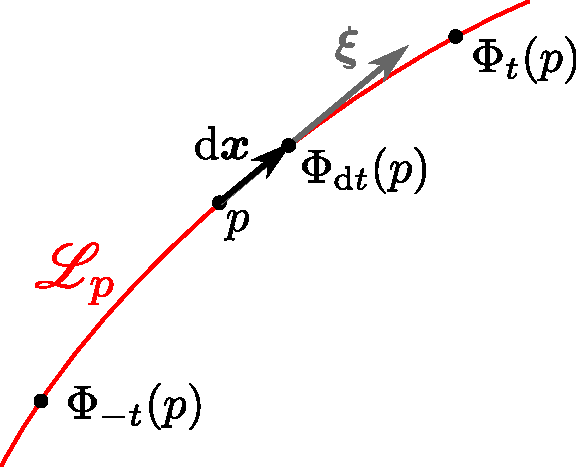
\includegraphics[height=0.25\textheight]{def_orbit_group.pdf}}
\caption[]{\label{f:neh:orbit_group} \footnotesize
Orbit $\Li_p$ of a point $p$ under the action $\Phi$ of a 1-dimensional Lie group, parameterized
by $t\in\R$. The tangent vector $\w{\xi} = \left. \D\w{x}/\D t \right| _{\Li_p}$ is the group
generator associated with this parameter.}
\end{figure}

Given a spacetime $(\M,\w{g})$ and a 1-dimensional Lie group $G$, one
says that $G$ is a
\defin{symmetry group}\index{symmetry!group}\index{group!symmetry --}
or a \defin{isometry group}\index{isometry!group}\index{group!isometry --}
of $(\M,\w{g})$, or equivalently that
$(\M,\w{g})$ is
\defin{invariant under the action of}\index{invariance!under a group action} $G$,
iff there is an action $\Phi$ of $G$ on $\M$
such that for any value of the parameter $t$ of $G$,
$\Phi_t$ is an \defin{isometry}\index{isometry} of $(\M,\w{g})$, i.e. $\Phi_t$
preserves the ``scalar products'' (and hence the ``distances'')
in the following sense: for any $p\in\M$ and any pair of points $(q,r)$
infinitely close to $p$, one has
\be \label{e:neh:isometry_dx}
    \left.\w{g}\right| _{\Phi_t(p)}(\D\w{x}', \D\w{y}') =
        \left.\w{g}\right| _{p}(\D\w{x}, \D\w{y}) ,
\ee
for the infinitesimal displacement vectors $\D\w{x} := \vp{pq}$, $\D\w{y} := \vp{pr}$,
$\D\w{x}' := \vp{\Phi_t(p)\Phi_t(q)}$ and $\D\w{y}' := \vp{\Phi_t(p)\Phi_t(r)}$
(cf. Sec.~\ref{s:fra:spacetime}).
Now, by definition, $\D\w{x}'$ is nothing but the pushforward
of the vector $\D\w{x}\in T_p\M$ to the tangent space
$T_{\Phi_t(p)}\M$ by the map $\Phi_t$
(cf. Sec.~\ref{s:bas:Lie_der_vector} of Appendix~\ref{s:bas}),
and similarly $\D\w{y}'$ is the pushforward of $\D\w{y}$ by $\Phi_t$:
\[
    \D\w{x}' = \Phi_{t*}(\D\w{x}) \quad\mbox{and}\quad
    \D\w{y}' = \Phi_{t*}(\D\w{y}) .
\]
By rescaling by infinitely small parameters (using the bilinearity of $\w{g}$),
it is clear that (\ref{e:neh:isometry_dx})
holds for finite vectors as well, so that we may say that $\Phi_t$ is an
isometry of $(\M,\w{g})$ iff
\be \label{e:neh:isometry}
    \forall p\in\M,\  \forall (\w{u},\w{v}) \in (T_p\M)^2,\quad
    \left. \w{g}\right| _{\Phi_t(p)} \left(\Phi_{t*}\w{u}, \Phi_{t*}\w{v}\right) =
    \left. \w{g}\right| _{p} (\w{u},\w{v}) ,
\ee
where $\Phi_{t*} \w{u}$ (resp. $\Phi_{t*} \w{v}$) is the pushforward of the vector
$\w{u}\in T_p\M$ (resp. $\w{v}\in T_p\M$)
to the tangent space $T_{\Phi_t(p)}\M$ by $\Phi_t$ [cf. Eq.~(\ref{e:bas:def_Phi_eps})].
Given the definition (\ref{e:bas:def_pullback}) of the pullback of
a bilinear form, we may reexpress the isometry condition (\ref{e:neh:isometry})
in terms of the
pullback of $\w{g}$ by $\Phi_t$:
\be \label{e:neh:isometry_pullback}
    \Phi_t^*\w{g} = \w{g} .
\ee
This is equivalent to the vanishing of the Lie derivative
of $\w{g}$ along the generators of $G$:
\begin{prop}[characterization of continuous spacetime isometries]
A 1-dimensional Lie group $G$
is a symmetry group of the spacetime $(\M,\w{g})$ iff the Lie derivative
of the metric tensor along a generator $\w{\xi}$ of $G$
vanishes identically:
\be \label{e:neh:Lie_xi_g}
    \encadre{\Lie{\xi}\w{g} = 0 } .
\ee
The vector field $\w{\xi}$ is then called a \defin{Killing vector}\index{Killing!vector field}
of $(\M,\w{g})$, Eq.~(\ref{e:neh:Lie_xi_g}) being equivalent to the
so-called
\defin{Killing equation}\index{Killing!equation}:
\be \label{e:neh:Killing_equation}
    \encadre{ \nabla_\alpha \xi_\beta + \nabla_\beta \xi_\alpha = 0 }.
\ee
\end{prop}
\begin{proof}
According the definition (\ref{e:bas:def_Lie_der_covar}) of the Lie
derivative\index{Lie!derivative}, we have
\[
    \Lie{\xi} \w{g} := \lim_{t \rightarrow 0} \frac{1}{t}
    \left( \Phi_t^*\w{g} - \w{g} \right) .
\]
The isometry condition
(\ref{e:neh:isometry_pullback}) implies then
$\Lie{\xi}\w{g} = 0$. The reverse is true by integration.
The equivalence between Eqs.~(\ref{e:neh:Lie_xi_g})
and (\ref{e:neh:Killing_equation}) immediately results from
expression~(\ref{e:bas:Lie_g_Killing}) for the Lie derivative of
$\w{g}$.
\end{proof}

\begin{prop}[isometry in adapted coordinates]
\label{p:neh:isometry_adapt_coord}
In terms of the components $g_{\alpha\beta}$ of $\w{g}$ with respect to
coordinates $(x^\alpha) = (t,x^1,\ldots,x^{n-1})$ adapted to the Killing vector $\w{\xi}$,
i.e. such that $\w{\xi} = \wpar_t$, the isometry condition (\ref{e:neh:Lie_xi_g})
is equivalent to
\be \label{e:neh:dgabdt_zero}
    \der{g_{\alpha\beta}}{t} = 0 .
\ee
$t$ is then called an \defin{ignorable coordinate}\index{ignorable coordinate}\index{coordinate!ignorable --}.
\end{prop}
\begin{proof}
This is a direct consequence of the identity (\ref{e:bas:Lie_adapted}).
\end{proof}


\subsection{Definition and examples of Killing horizons} \label{s:neh:def_Killing_hor}

\begin{greybox}
A \defin{Killing horizon}\index{Killing!horizon}\index{horizon!Killing --} is
a connected null hypersurface $\Hor$ in a spacetime $(\M,\w{g})$ admitting a
Killing vector field $\w{\xi}$ such that, on $\Hor$, $\w{\xi}$ is
normal to $\Hor$.
\end{greybox}

Thus the existence of a Killing horizon requires that the spacetime $(\M,\w{g})$ has
some continuous symmetry
(usually stationarity), namely that it is invariant under the action of a
1-parameter group, as described in Sec.~\ref{s:neh:symmetries}.
Since the normal to a null hypersurface is tangent to its null geodesic
generators and a Killing vector is tangent to the orbits of the isometry group,
a definition equivalent to the above one is:
\begin{greybox}
A \defin{Killing horizon} is a connected null
hypersurface $\Hor$ whose null geodesic generators are orbits of a
1-parameter group of isometries of $(\M,\w{g})$.
\end{greybox}

Its immediately follows from the definition that the Killing vector $\w{\xi}$ is non-vanishing
on $\Hor$ (a normal to a hypersurface cannot vanish) and is null on $\Hor$:
\be \label{s:neh:xi_on_KH}
    \left. \w{\xi} \right| _{\Hor} \not= 0
    \qquad\mbox{and}\qquad
    \left. \w{\xi}\cdot\w{\xi} \right| _{\Hor} = 0 .
\ee

We shall see in Chap.~\ref{s:sta} that in a stationary spacetime, under some rather generic
hypotheses, a (connected part of a) black hole
event horizon must be a Killing horizon.

\begin{figure}
\centerline{\includegraphics[width=0.6\textwidth]{def_hplaneKilling-boost.pdf}}
\caption[]{\label{f:neh:hplaneKilling-boost} \footnotesize
Null half-hyperplanes $\Hor^+$ and $\Hor^-$ as Killing horizons for the
Killing vector field $\w{\xi}=x \wpar_t + t \wpar_x$ generating Lorentz boosts
in Minkowski spacetime. The green lines are the null geodesic generators of
$\Hor$, while the thick black line (actually a 2-plane) marks the location
where $\w{\xi}$ vanishes.}
\end{figure}

\begin{example}[null hyperplane as a translation-Killing horizon]
\label{x:neh:transKH}
Let us consider the null hyperplane of Minkowski spacetime $\Hor$ discussed in
Examples~\ref{x:def:null_hyp}, \ref{x:def:null_hyp2} and \ref{x:def:null_hyp3}
of Chap.~\ref{s:def}.
$\Hor$ is defined by the equation $t=x$. The vector field
\be
    \w{\xi} := \wpar_t + \wpar_x
\ee
is a Killing vector of Minkowski spacetime: $\w{\xi}$ is the generator of
translations in the direction $\wpar_t + \wpar_x$, and these translations constitute a
1-dimensional subgroup of the Poincaré group --- the symmetry group of Minkowski
spacetime. We note that $\w{\xi}$ coincides with the null vector $\wl$
defined by Eq.~(\ref{e:def:wl_null_hyperplane}). Since $\wl$ is
normal to $\Hor$, we conclude immediately that $\Hor$ is a Killing horizon
with respect to $\w{\xi}$.
\end{example}

\begin{example}[null hyperplane as a boost-Killing horizon]
\label{x:neh:boostKH}
Let us consider the same null hyperplane $\Hor$ as above, but
with another Killing vector of Minkowski spacetime:
\be \label{e:neh:boost-Killing}
    \w{\xi} := x \wpar_t + t \wpar_x .
\ee
This vector is the
generator of the 1-parameter group of Lorentz boosts\index{boost} in the $(t,x)$ plane.
On $\Hor$ we have (cf. Fig.~\ref{f:neh:hplaneKilling-boost}):
\[
    \w{\xi} \equalH t (\wpar_t + \wpar_x) \equalH t \, \wl ,
\]
where $\wl$ is the null normal to $\Hor$ defined by
Eq.~(\ref{e:def:wl_null_hyperplane}) and the notation $\equalH$ means that the equality holds only on $\Hor$. We conclude that $\w{\xi}$ is a normal to
the null hypersurface $\Hor$ as soon as $t\not=0$. Therefore, we may split
$\Hor\setminus\{t=0\}$ in two open half-hyperplanes:
\be \label{e:neh:boost-Killing_hor}
    \Hor^+ := \{ p\in\Hor,\quad t(p) > 0 \} \quad\mbox{and}\quad
    \Hor^- := \{ p\in\Hor,\quad t(p) < 0 \} ,
\ee
so that each of them is a Killing horizon with
respect to $\w{\xi}$ (cf. Fig.~\ref{f:neh:hplaneKilling-boost}).
\end{example}

\begin{example}[null hyperplane as a null-rotation-Killing horizon]
\label{x:neh:nullrotKH}
Another example of Killing horizon is still provided by the null hyperplane
$\Hor$ considered above, but this time with the Killing vector
\be \label{e:neh:xi_null_rotation}
   \w{\xi} := y( \wpar_t + \wpar_x ) + (t-x)\wpar_y .
\ee
This vector is indeed the generator of
null rotations leaving the plane
$\mathrm{Span}(\wl,\wpar_z)$ strictly invariant (cf. e.g. Sec.~6.4.5 of
Ref.~\cite{Gourg13}), $\wl$ being the null normal of $\Hor$ defined by
Eq.~(\ref{e:def:wl_null_hyperplane}). These null rotations form a
1-dimensional subgroup of the Lorentz group, and thereby
a symmetry group of Minkowski spacetime. It is also immediate to check that
the vector defined by (\ref{e:neh:xi_null_rotation}) obeys
Killing equation (\ref{e:neh:Killing_equation}).
On $\Hor$, $t-x=0$, so that
(\ref{e:neh:xi_null_rotation}) reduces to
\[
    \w{\xi}  \equalH y ( \wpar_t + \wpar_x )  \equalH y \, \wl .
\]
It follows that $\w{\xi}$ is a null normal to $\Hor$ as soon as $y\not=0$.
We may then split $\Hor\setminus\{y=0\}$ in two open half-hyperplanes:
\[
    \Hor_1 := \{ p\in\Hor,\quad y(p) < 0 \} \quad\mbox{and}\quad
    \Hor_2 := \{ p\in\Hor,\quad y(p) > 0 \} ,
\]
each of them being a Killing horizon with
respect to $\w{\xi}$ (cf. Fig.~\ref{f:neh:hplaneKilling-nullrot}).
\end{example}

\begin{figure}
\centerline{\includegraphics[width=0.6\textwidth]{def_hplaneKilling-nullrot.pdf}}
\caption[]{\label{f:neh:hplaneKilling-nullrot} \footnotesize
Null half-hyperplanes $\Hor_1$ and $\Hor_2$ as Killing horizons for the
Killing vector field $\w{\xi}=y( \wpar_t + \wpar_x ) + (t-x)\wpar_y$
generating null rotations
in Minkowski spacetime. The green lines are the null geodesic generators of
$\Hor$, while the thick black line (actually a 2-plane) marks the location
where $\w{\xi}$ vanishes.}
\end{figure}

\begin{example}[light cone as a counter-example]
The future light cone introduced in Example~\ref{x:def:light_cone} of Chap.~\ref{s:def} is \emph{not} a
Killing horizon of Minkowski spacetime: it is invariant under the action
of the Lorentz group, but its null generators are not invariant
under the action of a single 1-dimensional subgroup of the Lorentz group.
Actually the future light cone is an example of a more general structure,
which Carter has termed a
\defin{local isometry horizon}\index{local!isometry horizon}\index{isometry!horizon}\index{horizon!local isometry --} \cite{Carte67,Carte69}: a null hypersurface that is invariant under
some group $G$ of isometries (here: the Lorentz group) and such that each null
geodesic generator is an orbit of some 1-dimensional subgroup of $G$,
this subgroup being not necessarily the same from one null generator to the next
(here: using Minkowskian spherical
coordinates $(t,r,\th,\ph)$,
the null geodesic generator through the point of coordinates $(1,1,\th_0,\ph_0)$
is the orbit of this point under the subgroup of boosts in the plane
$(\th,\ph) = (\th_0,\ph_0)$). A Killing horizon is a local isometry horizon
for which $\dim G = 1$.
\end{example}


\begin{example}[Schwarzschild horizon] \label{x:neh:Schwarz_KH}
Given the expression (\ref{e:def:wl_Schw_hor}) for the null normal $\wl$
of the family of hypersurfaces $\Hor_u$ and the fact that the Schwarzschild
horizon $\Hor$ is defined by $r=2m$, we have
\be \label{e:neh:wl_wpt_Schw_hor}
    \wl \equalH \wpar_t .
\ee
Now the vector field $\wpar_t$ is clearly a Killing vector of metric $\w{g}$
as given by (\ref{e:def:Schw_metric}), since none of the metric components
$g_{\alpha\beta}$ depends upon $t$. Hence (\ref{e:neh:wl_wpt_Schw_hor})
shows that the Schwarzschild horizon is a Killing horizon. By the way,
Eq.~(\ref{e:neh:wl_wpt_Schw_hor}) was our motivation for the choice of the
null normal $\wl$ performed in Example~\ref{x:def:Schw_hor2} of Chap.~\ref{s:def}.
\end{example}

\begin{hist}
The concept of Killing horizon has been introduced by Brandon Carter\index[pers]{Carter, B.} in
1966 \cite{Carte66,Carte67} and developed in an article published in
1969 \cite{Carte69}. The properties of Killing horizons have been
studied in detail by Robert H. Boyer\index[pers]{Boyer, R.H.},
in an article prepared posthumously from his notes
by J.~Ehlers and J.L.~Stachel and published in 1969 \cite{Boyer69},
leading to the concept of \emph{bifurcate Killing horizon}, to be discussed in
Sec.~\ref{s:sta:bifur_Killing_hor} (cf. the historical note on p.~\pageref{h:sta:Boyer}).
\end{hist}

\subsection{Killing horizons as non-expanding horizons}

Let us consider a cross-section $\Sp$ of a Killing horizon $\Hor$ with respect to a Killing vector $\w{\xi}$
and let us select the null normal $\wl$ to coincide with $\w{\xi}$ on $\Hor$:
$\wl \equalH \w{\xi}$. Since $\w{\xi}$ is an isometry generator, it is pretty obvious that the
metric $\w{q}$ induced by $\w{g}$ on $\Sp$ will not evolve when Lie dragged along $\w{\xi}$ and
hence that the deformation rate $\w{\Theta}$ of $\Sp$ along $\w{\xi}$, as defined by
Eq.~(\ref{e:def:Theta}), vanishes identically.
One can establish this rigorously from expression~(\ref{e:def:Theta_q_nabla_l}) for $\w{\Theta}$.
Indeed, without any loss of generality, we may express
the null vector field $\wl$ in a neighborhood of $\Hor$ as $\wl = \w{\xi} + u \w{w}$ where $u$ is a scalar field
defining $\Hor$ as the level set $u=0$, i.e. a scalar field obeying Eqs.~(\ref{e:def:Hor_u_zero})-(\ref{e:def:du_not_zero}). Then Eq.~(\ref{e:def:Theta_q_nabla_l}) leads to
\[
    \Theta_{\alpha\beta}  = q^\mu_{\ \, \alpha} q^\nu_{\ \, \beta} \nabla_\mu \xi_\nu
        + \underbrace{u}_{0} q^\mu_{\ \, \alpha} q^\nu_{\ \, \beta} \nabla_\mu w_\nu
        + \underbrace{q^\mu_{\ \, \alpha} \nabla_\mu u}_{0} \; q^\nu_{\ \, \beta}  w_\nu
        = q^\mu_{\ \, \alpha} q^\nu_{\ \, \beta} \nabla_\mu \xi_\nu ,
\]
where the identifications with zero hold on $\Sp$, the second one because $u$ is constant (being equal to zero) on
$\Sp$. Now thanks to the Killing equation (\ref{e:neh:Killing_equation}), $q^\mu_{\ \, \alpha} q^\nu_{\ \, \beta} \nabla_\mu \xi_\nu$ is an antisymmetric tensor field, while $\Theta_{\alpha\beta}$ is symmetric
(cf. Sec.~\ref{s:def:deformation_shear}). It follows that $\Theta_{\alpha\beta}=0$.
In view of the scaling law (\ref{e:def:rescale_deform_shear}), we can extend this result to the deformation rate
of $\Sp$ along any null normal to $\Hor$ and therefore state:

\begin{prop}[vanishing of the deformation rate of cross-sections of a Killing horizon]
On a Killing horizon $\Hor$,
the deformation rate $\w{\Theta}$ of any cross-section along any null normal $\wl$
is identically zero:
\be \label{e:neh:Theta_zero_KillingH}
   \encadre{ \w{\Theta} = 0 }.
\ee
This implies that the expansion of $\Hor$ along any null normal $\wl$ vanishes:
\be
    \theta_{(\wl)} = 0 .
\ee
\end{prop}
In view of the definition of a non-expanding horizon (cf. Sec.~\ref{s:neh:def}),
an immediate corollary is
\begin{prop}[Killing horizons as non-expanding horizons]
Any Killing horizon with closed-manifold cross-sections is a non-expanding horizon.
\end{prop}

\begin{remark}
$\w{\Theta}$ vanishes for any Killing horizon [Eq.~(\ref{e:neh:Theta_zero_KillingH})], while to get the same result on a generic non-expanding horizon, one has to assume that the null convergence condition holds on $\Hor$
(Property~\ref{p:neh:invariance_of_2metric}).
\end{remark}

\subsection{Expressions of the non-affinity coefficient}

Let $\kappa$ be the non-affinity coefficient
(cf. Sec.~\ref{s:def:geod_gener} and \ref{s:geo:gener_param})
of the null normal $\wl$ coinciding with the Killing vector $\w{\xi}$
on a Killing horizon $\Hor$. According to the definition
(\ref{e:def:wl_geod_kappa}), we have
\be \label{e:neh:xi_nab_xi_kappa}
    \wnab_{\w{\xi}}\, \w{\xi} \equalH \kappa \, \w{\xi} .
\ee
Let us consider the metric dual of this relation, i.e.
$\xi^\mu \nabla_\mu \xi_\alpha \equalH \kappa \, \xi_\alpha$,
and use the Killing equation (\ref{e:neh:Killing_equation}) as
$\nabla_\mu \xi_\alpha = - \nabla_\alpha \xi_\mu$; we get
\[
    \xi^\mu \nabla_\alpha \xi_\mu \equalH - \kappa \, \xi_\alpha .
\]
Now $\xi^\mu \nabla_\alpha \xi_\mu = 1/2 \, \nabla_\alpha (\xi_\mu \xi^\mu)$.
Hence
\be
    \nabla_\alpha (\xi_\mu \xi^\mu) \equalH - 2 \kappa \, \xi_\alpha.
\ee
Since $\xi_\mu \xi^\mu = \w{\xi}\cdot\w{\xi}$ is a scalar field, we may
replace the covariant derivative by the differential:
\be \label{e:neh:dxi2_kappa}
    \encadre{ \dd (\w{\xi}\cdot\w{\xi}) \equalH - 2 \kappa \, \uu{\xi} } .
\ee

\begin{remark}
If $u:=\w{\xi}\cdot\w{\xi}$ is a regular scalar field in the vicinity of $\Hor$, in the sense
that $\dd u \neq 0$, it is not surprising to have $\dd u$ proportional
to $\uu{\xi}$ on $\Hor$. Indeed, if $\dd u \neq 0$, the hypersurface $\Hor$ can be considered
as the level set $u=0$ for $\w{\xi}$ is null on $\Hor$ (cf. Sec.~\ref{s:def:hypsurf_level}).
It follows that the gradient $\vw{\nabla} u$ must be collinear to
the normal $\w{\xi}$ to $\Hor$ (cf. Sec.~\ref{s:def:null_normal}) or equivalently
$\dd u \equalH \alpha\, \uu{\xi}$. Equation~(\ref{e:neh:dxi2_kappa}) simply shows
that the proportionality factor is $\alpha = -2\kappa$.
\end{remark}

Another interesting relation is obtained from the Frobenius theorem\index{Frobenius!theorem}
applied to $\w{\xi}$. Indeed, since on $\Hor$, $\w{\xi}$ is normal to a hypersurface
($\Hor$), the Frobenius theorem in its dual formulation
(see e.g.
Theorem B.3.2 in Wald's textbook \cite{Wald84} or Theorem C.2 in
Straumann's textbook \cite{Strau13}) states that there exists a 1-form
$\w{a}$ such that
\be
    \dd \uu{\xi} \equalH \w{a} \wedge \uu{\xi} ,
\ee
or equivalently
\be \label{e:neh:Frobenius_xi}
  \nabla_\alpha \xi_\beta - \nabla_\beta \xi_\alpha \equalH
  a_\alpha \, \xi_\beta -  a_\beta  \, \xi_\alpha  .
\ee

\begin{remark}
In the case of the vector $\wl$, which is normal to $\Hor$ by definition,
the Frobenius identity is
Eq.~(\ref{e:def:ext_der_wl_comp}): $\nabla_\alpha \el_\beta - \nabla_\beta \el_\alpha =
  \nabla_\alpha \rho \, \el_\beta -  \nabla_\beta \rho \, \el_\alpha$.
Since $\wl \equalH \w{\xi}$, we may write
\[
  \nabla_\alpha \el_\beta - \nabla_\beta \el_\alpha \equalH
  \nabla_\alpha \rho \, \xi_\beta -  \nabla_\beta \rho \, \xi_\alpha .
\]
But in general,  $\nabla_\alpha \el_\beta \not= \nabla_\alpha \xi_\beta$ on $\Hor$,
since $\wl$ and $\w{\xi}$ do not coincide outside $\Hor$. Accordingly, one
cannot identify the left-hand side of the above equation with the left-hand side
of Eq.~(\ref{e:neh:Frobenius_xi}), so that the 1-form $\w{a}$ is \emph{not} $\wnab\rho$.
\end{remark}

Thanks to the Killing equation (\ref{e:neh:Killing_equation}), we may reshape
(\ref{e:neh:Frobenius_xi}) to
\be \label{e:neh:Frobenius_xi_Killing}
    2 \nabla_\alpha \xi_\beta \equalH
  a_\alpha \, \xi_\beta -  a_\beta \, \xi_\alpha  .
\ee
Contracting this relation with $\w{\xi}$, we get
\[
   2 \xi^\mu \nabla_\mu \xi_\alpha \equalH a_\mu \xi^\mu  \, \xi_\alpha
    -  \underbrace{\xi_\mu \xi^\mu}_{\equalH 0} \, a_\alpha .
\]
In view of Eq.~(\ref{e:neh:xi_nab_xi_kappa}), the left-hand side of this
equation is $2\kappa \xi_\alpha$. Hence we obtain
\be \label{e:neh:a_xi_2_kappa}
    a_\mu \xi^\mu \equalH 2 \kappa .
\ee
Besides, taking the square of (\ref{e:neh:Frobenius_xi_Killing}) leads to
\bea
    4 \nabla_\mu \xi_\nu \, \nabla^\mu \xi^\nu & \equalH &
        \left( a_\mu \xi_\nu -  a_\nu \xi_\mu \right)
       \left( a^\mu \xi^\nu - a^\nu \xi^\mu \right)
       \nonumber \\
       & \equalH & a_\mu a^\mu
        \underbrace{ \xi_\nu \xi^\nu}_{\equalH 0}
        - \underbrace{a_\mu \xi^\mu}_{2\kappa}
         \underbrace{a_\nu \xi^\nu}_{2\kappa}
        - \underbrace{a_\nu \xi^\nu}_{2\kappa}
            \underbrace{a_\mu \xi^\mu}_{2\kappa}
        + a_\nu  a^\nu
        \underbrace{ \xi_\mu \xi^\mu}_{\equalH 0}
        \equalH  - 8 \kappa^2 , \nonumber
\eea
where we have used Eq.~(\ref{e:neh:a_xi_2_kappa}).
Hence
\be \label{e:neh:kappa2}
    \encadre{\kappa^2 \equalH - \frac{1}{2}
        \nabla_\mu \xi_\nu \nabla^\mu \xi^\nu } .
\ee
This is an explicit expression of $\kappa$ in terms of the Killing vector
field $\w{\xi}$.
However, in actual calculations, it is generally preferable to employ
formula~(\ref{e:neh:dxi2_kappa}) to evaluate $\kappa$, because it does not involve
the computation of any covariant derivative, contrary to formula~(\ref{e:neh:kappa2}).


\subsection{The zeroth law of black hole dynamics} \label{s:neh:zeroth_law}

We are going to derive a result of great importance for black hole physics,
namely the non-affinity coefficient $\kappa$ discussed above
is constant on a Killing horizon, provided some mild energy condition holds.

Let us denote by $\wl$ the null normal to $\Hor$ that coincides with
the Killing vector field: $\wl \equalH \w{\xi}$. The vector field
$\wl$ is then a symmetry generator on $\Hor$, which implies
\be \label{e:neh:kappa_const_along_L}
    \Lie{\el} \kappa = 0 .
\ee
This means that $\kappa$ is constant along any field line of $\wl$ (i.e. any
null geodesic generator of $\Hor$). It could however vary from one field line to another.
To prove that this is not the case, let us consider a complete cross-section
$\Sp$ of $\Hor$ and show that $\kappa$ is constant on $\Sp$. The starting
point is applying the contracted Ricci identity (\ref{e:def:contract_Ricci_ident}),
which is a 1-form, to a generic vector field $\w{v}$ tangent to $\Sp$,
i.e. contract (\ref{e:def:contract_Ricci_ident}) with $v^\alpha$. Since $\el_\mu v^\mu = 0$, we get
\be \label{e:def:0law_prov}
    v^\nu \nabla_\mu \Theta^\mu_{\ \, \nu}  + v^\nu \el^\mu \nabla_\mu \omega_\nu
       - v^\mu \nabla_\mu \left( \theta_{(\wl)} + \kappa \right)
        + \left( \theta_{(\wl)} + \kappa \right) \omega_\mu v^\mu
        - \Theta_{\mu\nu} v^\mu k^\sigma \nabla_\sigma \el^\nu
     = R_{\mu\nu} \el^\mu v^\nu .
\ee
Now, since $\Hor$ is a Killing horizon, we have $\w{\Theta}=0$ [Eq.~(\ref{e:neh:Theta_zero_KillingH})] and in particular
$\theta_{(\wl)} =0$, so that many terms in the above equation vanish.
The term $\nabla_\mu \Theta^\mu_{\ \, \nu}$ requires some special care though, because it potentially
involves derivatives of $\vw{\Theta}$ in directions transverse\footnote{Recall that, in our setting, tensor fields are extended beyond $\Hor$ by considering $\Hor$ as the element $u=0$ of a
family $(\Hor_u)_{u\in\R}$ of null hypersurfaces (cf. Sec.~\ref{s:def:null_normal}). We cannot assume
that each $\Hor_u$ is a Killing horizon (because typically the scalar $\w{\xi}\cdot\w{\xi}$ vanishes on
a single hypersurface, not on an open subset of $\M$), so
$\vw{\Theta}$ is a priori not zero outside $\Hor$.}
 to $\Hor$. Let us then introduce
in the vicinity of $\Sp$ a spacetime coordinate system $(x^\alpha) = (u,v,x^2,\ldots,x^{n-1})$
adapted to $\Sp$, as the one introduced in Sec.~\ref{s:def:def_expansion}
[cf. Eq.~(\ref{e:def:l_wpar_v})], namely a coordinate system such that $\Sp$
is the set $(u,v) = (0,0)$. Then the components of $\vw{\Theta}$ with respect
to $(x^\alpha)$ necessarily verify $\Theta^0_{\ \, \alpha} = 0$ and
$\Theta^1_{\ \, \alpha} = 0$. Indeed, since $\vw{\Theta}$ is a tensor field
tangent to $\Sp$, on which $u$ and $v$ are constant,
we have $\Theta^\mu_{\ \, \alpha} \nabla_\mu u = 0$ and
$\Theta^\mu_{\ \, \alpha} \nabla_\mu v= 0$ with $\nabla_\mu u = \partial_\mu u = \delta^0_{\ \, \mu}$
and $\nabla_\mu v = \partial_\mu v = \delta^1_{\ \, \mu}$ by definition of $(x^\alpha)$.
Expressing the covariant derivative via Eq.~(\ref{e:bas:der_cov_coord}), we get
\[
    \nabla_\mu \Theta^\mu_{\ \, \nu} = \partial_a \Theta^a_{\ \, \nu}
        + \Gamma^\mu_{\ \, \mu\sigma} \Theta^\sigma_{\ \, \nu}
        - \Gamma^\sigma_{\ \, \mu\nu}  \Theta^\mu_{\ \, \sigma} ,
\]
where the sum of the partial derivatives has been limited to the indices
$a\in\{2,\ldots,n-1\}$ since $\Theta^0_{\ \, \nu} = \Theta^1_{\ \, \nu} = 0$.
Given that the term $\partial_a \Theta^a_{\ \, \nu}$ involves only the variation
of $\vw{\Theta}$ in directions tangent to $\Sp$, we conclude that
$\nabla_\mu \Theta^\mu_{\ \, \nu} = 0$ if $\vw{\Theta} = 0$ on $\Sp$.
Hence, for a Killing horizon,
Eq.~(\ref{e:def:0law_prov}) reduces to
\be \label{e:neh:zeroth_law_step1}
  (\el^\nu \nabla_\nu \omega_\mu + \kappa  \, \omega_\mu) v^\mu
    - v^\mu \nabla_\mu \kappa
    = R_{\mu\nu} \el^\mu v^\nu .
\ee
The terms in the parentheses are related to the Lie derivative
of $\w{\omega}$ along $\wl$; indeed formula (\ref{e:bas:Lie_der_comp_nab}) gives:
\bea
    \Liec{\el}\omega_\mu & =  & \el^\nu \nabla_\nu \omega_\mu + \omega_\nu \nabla_\mu \el^\nu
     = \el^\nu \nabla_\nu \omega_\mu + \omega_\nu \left( \Theta_\mu^{\ \, \nu}
     + \omega_\mu \el^\nu - \el_\mu k^\sigma \nabla_\sigma \el^\nu \right) \nonumber \\
     & = & \el^\nu \nabla_\nu \omega_\mu  + \kappa \omega_\mu - \omega_\nu \el_\mu k^\sigma \nabla_\sigma \el^\nu , \nonumber
\eea
where we have expressed $\nabla_\mu \el^\nu$ via Eq.~(\ref{e:def:nab_l_Theta}) and
have used $\Theta_\mu^{\ \, \nu} = 0$ and $\omega_\nu \el^\nu = \kappa$
[Eq.~(\ref{e:def:omega_l_kappa})].
Given that $\el_\mu v^\mu = 0$, Eq.~(\ref{e:neh:zeroth_law_step1})
becomes
\be  \label{e:neh:zeroth_law_step2}
  \langle \Lie{\el} \w{\omega}, \w{v} \rangle - \wnab_{\w{v}}\,  \kappa
    = \w{R}(\wl, \w{v}) .
\ee
It is judicious to
express $\Lie{\el}\w{\omega}$ in terms of $\Lie{\el}{}^{\Hor}\!\w{\omega}$,
where ${}^{\Hor}\!\w{\omega}$ is the restriction of $\w{\omega}$ to tangent vectors
to $\Hor$ (pullback to $\Hor$) introduced in Sec.~\ref{e:neh:induced_connection}.
The reason is that, contrary to $\w{\omega}$,
${}^{\Hor}\!\w{\omega}$ is a geometric quantity intrinsic to
$\Hor$ and $\wl$, independent of $\w{k}$ and hence of the cross-section $\Sp$
(cf. Property~\ref{p:neh:Hnab_l} and the discussion below it).
It has therefore to obey the spacetime symmetry generated by $\w{\xi} \equalH \wl$,
i.e. one has
\be \label{e:neh:Lie_l_Homeg_zero}
    \Lie{\el} {}^{\Hor}\!\w{\omega} = 0 .
\ee
Now, using the Leibniz rule twice, we get
\[
    \langle \Lie{\el} \w{\omega}, \w{v} \rangle = \Lie{\el}
    \underbrace{\langle \w{\omega}, \w{v} \rangle}_{\langle {}^{\Hor}\!\w{\omega}, \w{v} \rangle}
    - \underbrace{\langle \w{\omega}, \Lie{\el} \w{v} \rangle}_{\langle {}^{\Hor}\!\w{\omega}, \Lie{\el} \w{v} \rangle} = \langle \Lie{\el} {}^{\Hor}\!\w{\omega}, \w{v} \rangle ,
\]
where the idendities $\langle \w{\omega}, \w{v} \rangle = \langle {}^{\Hor}\!\w{\omega}, \w{v} \rangle$
and $\langle \w{\omega}, \Lie{\el} \w{v} \rangle =  \langle {}^{\Hor}\!\w{\omega}, \Lie{\el} \w{v} \rangle$
hold by the very definition of ${}^{\Hor}\!\w{\omega}$,
since $\w{v}$ and $\Lie{\el}\w{v}$ are tangent\footnote{$\Lie{\el}\w{v}$ is tangent to
$\Hor$ for both $\wl$ and $\w{v}$ are tangent to $\Hor$.}
to $\Hor$. It follows then from (\ref{e:neh:Lie_l_Homeg_zero}) that $\langle \Lie{\el} \w{\omega}, \w{v} \rangle = 0$; hence the
first term in Eq.~(\ref{e:neh:zeroth_law_step2}) vanishes identically and there remains
only:
\be \label{e:neh:DS_kappa_W}
    \wnab_{\w{v}} \, \kappa = - \w{R}(\wl, \w{v}) .
\ee

To go further, we shall assume the
\defin{null dominance condition}\index{null!dominance condition}\index{dominance!null -- condition} \cite{Racz08}, namely that there
exists a scalar field $f$ such that
\be \label{e:neh:null_dominant_cond}
  \encadre{  \begin{array}{ll}
    \mbox{the vector} \ \w{W} := - \vw{G}(\wl) - f \wl \ & \mbox{is future-directed null or timelike} \\
    & \mbox{for any future-directed null vector $\wl$}
    \end{array} } .
\ee
In the above equation, $\vw{G}$ stands for the type-$(1,1)$ tensor
associated by metric duality to the Einstein tensor\index{Einstein!tensor}
$\w{G}$ [Eq.~(\ref{e:bas:Einstein_tensor})], so that the expression of $\w{W}$
in index notation is [cf. Eq.~(\ref{e:bas:arrow_endo_index})]
\be \label{e:neh:def_W_index}
    W^\alpha = - G^\alpha_{\ \, \mu} \el^\mu - f \ell^\alpha .
\ee
Note that the null dominance condition implies the null convergence condition
(\ref{e:neh:null_energy_cond}) since
\be \label{e:neh:R_ll_W_l}
    \w{R}(\wl, \wl) = \w{R}(\wl, \wl) - \frac{R}{2} \underbrace{\w{g}(\wl, \wl)}_{0}
    + f \underbrace{\w{g}(\wl, \wl)}_{0}  =  \w{G}(\wl, \wl) + f \w{g}(\wl,\wl)
     =  - \w{W}\cdot\wl \geq 0 ,
\ee
the inequality holding because both $\w{W}$ and $\wl$ are future-directed
(cf. Lemma~\ref{p:fra:lem2}).

If gravity is described by general relativity, i.e. if the metric $\w{g}$
fulfills the Einstein equation (\ref{e:fra:Einstein_eq_G}), then
the null dominance condition with $f = \Lambda$ is
equivalent to the
\defin{null dominant energy condition}\index{null!dominant energy condition}\index{energy!condition!null dominant --}:
\be \label{e:neh:null_dominant_cond_T}
  \encadre{ \begin{array}{ll}
    \mbox{The vector} \ \w{W} := - \vw{T}(\wl) \ & \mbox{is zero or future-directed null or timelike} \\
    & \mbox{for any future-directed null vector $\wl$}
    \end{array} }_{\rm \, GR},
\ee
where $\w{T}$ is the energy-momentum tensor of matter and non-gravitational fields.
By continuity, the null dominant energy condition is implied by the standard
\defin{dominant energy condition}\index{dominant energy condition}\index{energy!condition!dominant --}:
\be
   \begin{array}{ll}
     \mbox{The vector} \ \w{W} := - \vw{T}(\w{u}) \ & \mbox{is zero or future-directed null or timelike} \\
    & \mbox{for any future-directed timelike vector $\w{u}$}
    \end{array}  .
\ee
Physically,
the dominant energy condition states that, with respect to any
observer (represented by its 4-velocity $\w{u}$, which is future-directed timelike),
the energy of matter and non-gravitational fields does not move faster than light
(see Ref.~\cite{Carte03} for an extended discussion).

\begin{remark}
While the name \emph{null convergence condition} for $\w{R}(\wl,\wl) \geq 0$
[Eq.~(\ref{e:neh:null_energy_cond})] is standard in the literature
(e.g. \cite{HawkiE73,Senov22a,SenovG15}), the name \emph{null dominance condition}
for (\ref{e:neh:null_dominant_cond}) is not standard. We are using it to
distinguish from the \emph{null dominant energy condition} (\ref{e:neh:null_dominant_cond_T}),
which a condition on the matter energy-momentum tensor, while (\ref{e:neh:null_dominant_cond})
is a pure geometrical identity, independent of the Einstein equation. In this way,
\emph{null dominance condition} is on the same footing as \emph{null convergence condition}.
\end{remark}

Coming back to Eq.~(\ref{e:neh:DS_kappa_W}), we note that its right-hand side
is nothing but the scalar product of the vector $\w{W}$
defined by Eq.~(\ref{e:neh:null_dominant_cond}) with $\w{v}$:
\[
    \w{W}\cdot\w{v} = - (\vw{G}(\wl) + f \wl)\cdot\w{v}
    = - \w{R}(\wl, \w{v}) + \left( \frac{R}{2} - f \right) \underbrace{\wl\cdot\w{v}}_{0}
    = - \w{R}(\wl, \w{v}) .
\]
If we assume the null dominance condition, the null convergence condition
holds, so that $\w{R}(\wl, \wl) = 0$ on $\Hor$ [Eq.~(\ref{e:neh:R_l_l_zero})].
Then, according to Eq.~(\ref{e:neh:R_ll_W_l}),
$\wl \cdot \w{W} = - \w{R}(\wl, \wl) = 0$.
This implies that the vector $\w{W}$ is tangent to $\Hor$. The latter
being a null hypersurface, $\w{W}$ must then be
either collinear to $\wl$ or spacelike (cf. Lemma~\ref{p:def:tangent_to_null_hyp} in Sec.~\ref{s:def:spacelike_sections}).
Now, according to the null dominance condition (\ref{e:neh:null_dominant_cond}),
$\w{W}$ cannot be
spacelike. We conclude that $\w{W}$ is collinear to $\wl$. Consequently,
we have $\w{W}\cdot\w{v} = 0$.
Hence the right-hand side of Eq.~(\ref{e:neh:DS_kappa_W}) vanishes identically
and we are left with $\wnab_{\w{v}} \, \kappa = 0$. Since $\w{v}$ is a generic
vector field tangent to $\Sp$ and $\Sp$ is connected (for it is a complete cross-section
of a Killing horizon, which is connected by definition),
this implies that
$\kappa$ is constant over $\Sp$. Given that $\kappa$ is
constant along each null geodesic generator of $\Hor$, this completes the demonstration
that $\kappa$ is constant over $\Hor$. More precisely, we have established
the following property:

\begin{prop}[zeroth law of black hole dynamics]
\label{p:neh:zeroth_law}
If the null dominance condition
(\ref{e:neh:null_dominant_cond})
is fulfilled on a Killing horizon $\Hor$ --- which is guaranteed in general relativity
if the null dominant energy condition (\ref{e:neh:null_dominant_cond_T}) holds ---, then the non-affinity coefficient $\kappa$
of the null normal coinciding with the Killing vector $\w{\xi}$ defining $\Hor$
is constant over $\Hor$:
\be \label{e:neh:zeroth_law}
    \encadre{\kappa = \mathrm{const}.}
\ee
\end{prop}
In the context of Killing horizons, the non-affinity coefficient $\kappa$ is
called the horizon's \defin{surface gravity}\index{surface!gravity},
for a reason to be detailed in Sec.~\ref{s:neh:surface_gravity},
and the result
(\ref{e:neh:zeroth_law}) is known as the
\defin{zeroth law of black hole dynamics}\index{zeroth law!of BH dynamics}. More precisely,
the zeroth law --- to be discussed in detail in Chap.~\ref{s:evo} ---
states that the surface gravity of a black hole in equilibrium is
constant and we shall see in Chap.~\ref{s:sta} that (any connected part of)
the event horizon of a black hole in equilibrium is a Killing horizon.


\begin{remark}
\label{r:neh:proof_zeroth_law}
The standard proof of the zeroth law, based on taking the covariant derivative
of Eq.~(\ref{e:neh:xi_nab_xi_kappa}) \cite{BardeCH73,Carte87,Wald84} or of Eq.~(\ref{e:neh:dxi2_kappa})
\cite{Heusl96} and on an identity expressing the second order derivative of
a Killing vector in terms of the Riemann tensor [Eq.~(\ref{e:neh:nabnab_xi_Riem}) below], is quite long (see
e.g. pp.~333-334 of Wald's textbook~\cite{Wald84} and the remark at the end of Sec.~5.5.2 of Poisson's
textbook \cite{Poiss04}). The proof presented above is shorter but it relies on
the concept of induced affine connection on a non-exanding horizon
(Sec.~\ref{e:neh:induced_connection}) and the associated rotation
1-form\index{rotation!1-form} ${}^{\Hor}\!\w{\omega}$ (cf.
Property~\ref{p:neh:Hnab_l}). This proof is actually adapted from a proof
presented by Damour\index[pers]{Damour, T.} \cite{Damou79,Damou82} (cf. historical note below); see
also Ref.~\cite{AshteBL01} for a related proof regarding isolated horizons.
\end{remark}

\begin{remark}
\label{r:neh:zero_law_wo_NDEC}
The constancy of $\kappa$ on a Killing horizon can also be proved without the
null dominance condition, but at the price of additional hypotheses:
either the Killing horizon $\Hor$ is part of a so-called bifurcate Killing horizon,
as we shall see in Sec.~\ref{s:neh:zeroth_law_bifur} (Property~\ref{p:neh:zeroth_law_bifur})
or the spacetime is axisymmetric, in addition to be stationary, and
the two Killing vectors associated
with stationarity and
axisymmetry are orthogonal to $(n-2)$-dimensional
surfaces \cite{Carte73b,RaczW96}.
\end{remark}

\begin{example}[null hyperplane as a translation-Killing horizon]
\label{x:neh:transKH_kappa}
For the null hyperplane $\Hor$ considered in Example~\ref{x:neh:transKH} as a Killing horizon with respect to the translation group along its normal, we have
$\kappa = 0$, as already noticed in Example~\ref{x:def:null_hyp3} of Chap.~\ref{s:def},
which is obviously constant over $\Hor$.
\end{example}

\begin{example}[null hyperplane as a boost-Killing horizon]
\label{x:neh:boostKH_kappa}
Let us consider each of the null half-hyperplanes $\Hor^+$
and $\Hor^-$ of Example~\ref{x:neh:boostKH}, which are Killing horizons with
respect to the boost Killing vector $\w{\xi} = x \wpar_t + t \wpar_x$. On
$\Hor^+$, the future-directed null normal coinciding with this Killing vector
is $\wl^+ = t\,  \wl$, $\wl$ being the geodesic null normal defined by
$\wl:= \wpar_t + \wpar_x$ [cf. Eq.~(\ref{e:def:wl_null_hyperplane})].
Using $\kappa_{\wl} = 0$ and the scaling law (\ref{e:def:rescale_kappa}),
we get the non-affinity
coefficient of $\wl^+$ as $\kappa_+= \wnab_{\wl} t = \partial_t t + \partial_x t$, i.e.
\[
    \kappa_+ = 1 .
\]
On $\Hor^-$, $\w{\xi}$ is past-directed (cf. Fig.~\ref{f:neh:hplaneKilling-boost}).
Sticking to future-directed null normals, we shall then consider $\Hor^-$
as a Killing horizon with respect to the Killing vector field $-\w{\xi}$.
The future-directed null normal coinciding with $-\w{\xi}$ on $\Hor^-$ is then
$\wl^- = -t\,  \wl$, from which we deduce the non-affinity
coefficient of $\wl^-$: $\kappa_-= \wnab_{\wl} (-t) = \partial_t (-t) + \partial_x (-t)$, i.e.
\[
    \kappa_- = -1 .
\]
We check that $\kappa_+$ (resp.  $\kappa_-$) is constant over the Killing horizon $\Hor^+$ (resp. $\Hor^-$), in agreement with Property~\ref{p:neh:zeroth_law}.
\end{example}

\begin{example}[null hyperplane as a null-rotation-Killing horizon]
\label{x:neh:nullrotKH_kappa}
In Example~\ref{x:neh:nullrotKH}, we have introduced the Killing horizons
$\Hor_1$ and $\Hor_2$ with respect to the null-rotation Killing vector
$\w{\xi} = y( \wpar_t + \wpar_x ) + (t-x)\wpar_y$ of Minkowski spacetime.
On $\Hor_1$, $\w{\xi}$ is past-directed (cf. Fig.~\ref{f:neh:hplaneKilling-nullrot}),
so that we shall actually consider $\Hor_1$
as a Killing horizon with respect to the Killing vector field $-\w{\xi}$.
The future-directed null normal coinciding with $-\w{\xi}$ on $\Hor_1$ is then
$\wl_1 = - y\, \wl$. Since it is clearly constant along the null geodesic generators
of $\Hor_1$, we have $\wnab_{\wl_1}\wl_1 = 0$, hence the
associated non-affinity coefficient vanishes: $\kappa_1 = 0$.
On $\Hor_2$, $\w{\xi}$ is future-directed (cf. Fig.~\ref{f:neh:hplaneKilling-nullrot})
and the null normal coinciding with it is $\wl_2 =  y\,  \wl$, whose non-affinity
coefficient is $\kappa_2 = 0$.
\end{example}

\begin{example}[Schwarzschild and Kerr horizons]
\label{x:neh:Schw_Kerr_kappa}
We have found in Example~\ref{x:def:Schw_hor3} of Chap.~\ref{s:def} [cf. Eq.~(\ref{e:def:kappa_Schw_hor})]
that on a Schwarzschild horizon $\kappa = 1/(4m)$,
which is clearly constant. But
this last feature is rather trivial since the Schwarzschild horizon is spherically
symmetric, so that no dependence of $\kappa$ on $\th$ nor $\ph$ could have been expected.
A much less trivial example is that of the event horizon of a Kerr black hole,
which we shall discuss in Chap.~\ref{s:ker}. This horizon is only axisymmetric,
so that a priori $\kappa$ could depend on $\th$. But it does not, as we shall
see in Sec.~\ref{s:ker:surf_grav}:
\[
    \kappa = \frac{\sqrt{m^2 - a^2}}{2m(m + \sqrt{m^2-a^2})} ,
\]
where $(m,a)$ are the two constant parameters of the Kerr solution. Note that for $a=0$,
we recover the Schwarzschild value: $\kappa= 1/(4m)$.
\end{example}

\begin{example}[Cubic Galileon black hole as a counter-example]
It has been found recently that the surface gravity of rotating stationary black holes
in a scalar-tensor theory of gravity known as the \emph{cubic Galileon}\index{cubic Galileon}
is not constant \cite{Grand24}.
This evades the zeroth law (Property~\ref{p:neh:zeroth_law})
because the null dominance condition is not satisfied by these solutions.
\end{example}

\begin{hist}
The constancy of $\kappa$ for a Killing horizon has been proven by Stephen Hawking\index[pers]{Hawking, S.W.}
in his lecture at the famous Les Houches School of summer 1972 \cite{Hawki73} (p.~43).
It has also been proven without requiring the null dominance condition, but
assuming axisymmetry and orthogonal transitivy\index{orthogonally transitive} (cf. Remark~\ref{r:neh:zero_law_wo_NDEC} on p.~\pageref{r:neh:zero_law_wo_NDEC}) by Brandon Carter\index[pers]{Carter, B.} in his lecture at the same summer
school
\cite{Carte73b} (Theorem 8, p.~167).
A third proof of the constancy of $\kappa$, using the null dominance condition,
has also been given in 1973 by James Bardeen\index[pers]{Bardeen, J.M.}, Brandon Carter and
Stephen Hawking
in their seminal article \emph{The Four Laws of Black Hole Mechanics}
\cite{BardeCH73}. Yet another proof has been provided in 1979 by Thibault Damour\index[pers]{Damour, T.}
\cite{Damou79,Damou82}, who developed a fluid-bubble approach to the dynamics of an event horizon.
In Damour's framework, the pullback of the 1-form  $-\w{\omega}/(8\pi)$ to the cross-section
$\Sp$ is considered as the momentum surface density of the fluid bubble and Eq.~(\ref{e:def:0law_prov})
is turned into a 2-dimensional Navier-Stokes equation (see e.g. Sec.~6.3 of Ref.~\cite{GourgJ06} for details), where $\kappa/(8\pi)$ plays the role of the
bubble's surface pressure, so that it must constant in equilibrium. As mentioned in Remark~\ref{r:neh:proof_zeroth_law},
the proof presented above is derived from Damour's one.
\end{hist}

\subsection{Classification of Killing horizons} \label{s:neh:classif_KH}

Since $\kappa$ is constant on a Killing horizon $\Hor$ (assuming the null dominance
condition), we may use it to classify Killing horizons in two
categories, depending whether $\kappa$ vanishes or not:
\begin{itemize}
\item if $\kappa = 0$, the Killing vector $\w{\xi}$ is a geodesic vector on $\Hor$
and $\Hor$ is called a \defin{degenerate Killing horizon}\index{degenerate!Killing horizon}\index{Killing!horizon!degenerate --};
\item if $\kappa \not=0$, $\w{\xi}$ is only a pregeodesic vector on $\Hor$
(cf. Sec.~\ref{s:geo:gener_param})
and $\Hor$ is called a \defin{non-degenerate Killing horizon}\index{non-degenerate!Killing horizon}\index{Killing!horizon!non-degenerate --}.
\end{itemize}

\begin{example}[Killing horizons in Minkowski spacetime]
In Minkowski spacetime, the null hyperplane as a translation-Killing horizon
(Example~\ref{x:neh:transKH_kappa}) and the two half-hyperplanes as
null-rotation-Killing horizons (Example~\ref{x:neh:nullrotKH_kappa}) are
degenerate Killing horizons, while the two half-hyperplanes as
boost-Killing horizons (Example~\ref{x:neh:boostKH_kappa}) are non-degenerate.
\end{example}

\begin{example}[Schwarzschild and Kerr horizons]
From the values of $\kappa$ given in Example~\ref{x:neh:Schw_Kerr_kappa},
we see that the Schwarzschild horizon and the Kerr horizon for
$a<m$ are non-degenerate Killing horizons, while the Kerr horizon for
$a=m$ is a degenerate one.
\end{example}

The next example regards the anti-de Sitter spacetime and will play some
role in the study of the extremal ($a=m$) Kerr black hole in Chap.~\ref{s:exk}.

\begin{figure}
\centerline{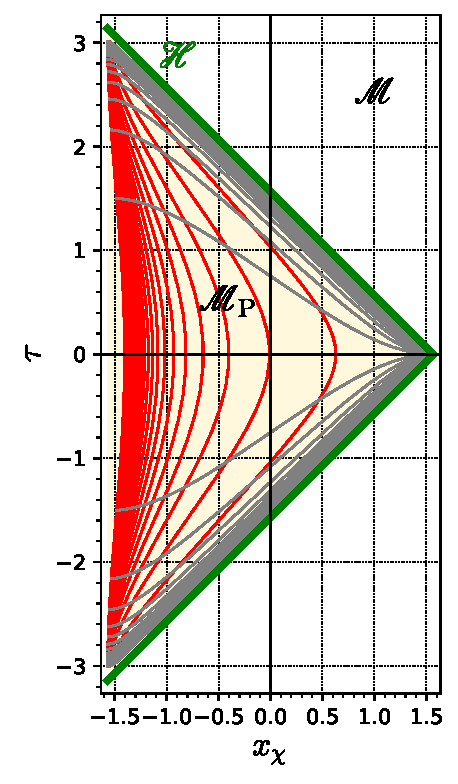
\includegraphics[width=0.35\textwidth]{neh_AdS_Poincare_patch.pdf}\ \qquad \
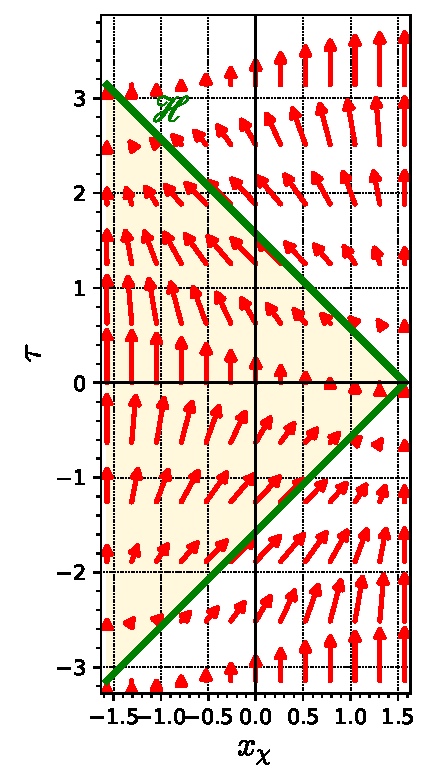
\includegraphics[width=0.35\textwidth]{neh_AdS_Killing_vec.pdf}
}
\caption[]{\label{f:neh:AdS_example} \footnotesize
\emph{Left:} 2-dimensional slice $(x,y)=(0,0)$ of the Poincaré patch $\M_{\rm P}$ of anti-de Sitter spacetime plotted in terms of the (global) coordinates $\tau$ and
$x_\chi := \chi \cos\ph$ (pale yellow region). From Eq.~(\ref{e:neh:Poincare_coord}),
$(x,y)=(0,0)$ implies $\th=\pi/2$ and $\ph=0$ or $\pi$, so that $x_\chi = \chi$
in the right half of the plot ($\ph=0$) and $x_\chi = - \chi$ in the left half
($\ph=\pi$). The plotted slice of $\M_{\rm P}$ is thus spanned by the
Poincaré coordinates $(t,u)$.
The red lines are curves of constant $u$, i.e. integral curves of
the coordinate vector field $\wpar_t = \w{\xi}$, with $u$ increasing from $0$ to $+\infty$
from the right to the left of the diagram. The grey lines are
curves of curves
of constant $t$, i.e. integral curves of the coordinate vector field $\wpar_u$,
with $t$ increasing from $-\infty$ to $+\infty$ from the bottom to the top
of the diagram. The Poincaré horizon $\Hor$ is depicted in green.
The two connected components $\Hor_-$ and $\Hor_+$ of $\Hor$
appear as straight line segments, since for $\th=\pi/2$
and $\ph\in\{0,\pi\}$, $u = 0 \iff \cos\tau = \pm \sin\chi$ ($+$ for $\ph=0$ and $-$ for $\ph=\pi$).
Note that the curves of constant $u$ tend to $\Hor$ when $u\to 0$, in agreement
with the characterization of $\Hor$ by $u=0$. The curves of constant
$t$ tend to $\Hor$ when $t\to \pm\infty$, which is expected as well since
the first line of Eq.~(\ref{e:neh:Poincare_coord}) and Eq.~(\ref{e:neh:AdS:def_u})
imply that $u\to 0$ for $t\to \pm\infty$.
\emph{Right:} Killing vector field $\w{\xi}$ defined by Eq.~(\ref{e:neh:AdS:def_xi})
on AdS$_{4}$; $\w{\xi}$ is timelike everywhere, except on the Poincaré
horizon $\Hor$, where it is null (and normal, and thus tangent, to $\Hor$).
\textsl{[Figures generated by the notebook \ref{s:sam:Poincare_hor}]}
}
\end{figure}

\begin{example}[Poincaré horizon in AdS$_{4}$] \label{x:neh:AdS}
The 4-dimensional \defin{anti-de Sitter spacetime}\index{anti-de Sitter spacetime} (AdS$_{4}$)
is $(\M,\w{g})$ with $\M\simeq \mathbb{R}^4$ and $\w{g}$ is the metric
whose components in the so-called \emph{global static coordinates}
$(\tau,r,\th,\ph)$ are given by
\be \label{e:neh:AdS4}
    \w{g} = \ell^2 \left[ - (1 + r^2) \, \dd \tau^2
    + \frac{\dd r^2}{1 + r^2} + r^2 \left( \dd\th^2 + \sin^2\th \, \dd\ph^2 \right) \right] ,
\ee
where $\ell$ is a positive constant.
Note that $\tau$ spans $\mathbb{R}$, $r$ spans $(0,+\infty)$,
while $(\th,\ph)$ are standard spherical coordinates on $\mathbb{S}^2$:
$\th\in(0,\pi)$ and $\ph\in(0,2\pi)$.
The metric (\ref{e:neh:AdS4}) is a solution
of the vacuum Einstein equation\index{Einstein!equation!vacuum --}\index{vacuum!Einstein equation} (\ref{e:fra:vac_Einstein_Lambda}) with
the negative cosmological constant $\Lambda = - 3/\ell^2$.
Using the so-called \emph{conformal coordinates} $(\tau,\chi,\th,\ph)$ with
$\chi := \arctan r \in (0,\pi/2)$, one gets
\be \label{e:neh:metrix_AdS_conformal}
   \w{g} = \frac{\ell^2}{\cos^2\chi} \left[ - \dd \tau^2
    + \dd \chi^2 + \sin^2\chi \left( \dd\th^2 + \sin^2\th \, \dd\ph^2 \right) \right] .
\ee
Note that $(\chi,\th,\ph)$ spans one half\footnote{It would span the whole hypersphere if
$\chi$ would run in all of $(0,\pi)$, instead of being limited to $(0,\pi/2)$.} of the hypersphere\index{hypersphere} $\mathbb{S}^3$.
Yet another set of coordinates commonly used in AdS$_{4}$ is \defin{Poincaré coordinates}\index{Poincaré!coordinates on AdS$_n$} $(t,x,y,u)$. They cover only a subpart
$\M_{\rm P}$ of $\M$ (cf. Fig.~\ref{f:neh:AdS_example}), usually called the \defin{Poincaré patch}\index{Poincaré!patch!of AdS$_4$} and defined by
\be \label{e:neh:def_Poincare_patch}
    \M_{\rm P}:\quad u > 0 \qand -\pi < \tau < \pi,
\ee
where $u$ is the following scalar field on $\M$:
\be \label{e:neh:AdS:def_u}
    u :=  \frac{\ell (\cos\tau - \sin\chi\sin\th\cos\ph)}{\cos\chi} .
\ee
On $\M_{\rm P}$, the Poincaré coordinates $(t,x,y,u)$ are related to the conformal coordinates
$(\tau,\chi,\th,\ph)$ by\footnote{See e.g. Ref.~\cite{BayonB07}.}
\be \label{e:neh:Poincare_coord}
    \left\{ \begin{array}{l}
    t = \frac{\ell \sin\tau}{\cos\tau - \sin\chi\sin\th\cos\ph} \\[1ex]
    x = \frac{\ell \sin\chi\sin\th\sin\ph}{\cos\tau - \sin\chi\sin\th\cos\ph} \\[1ex]
    y = \frac{\ell \sin\chi\cos\th}{\cos\tau - \sin\chi\sin\th\cos\ph} \\[1ex]
    u = \frac{\ell (\cos\tau - \sin\chi\sin\th\cos\ph)}{\cos\chi} .
    \end{array}\right.
\ee
The last line is simply (\ref{e:neh:AdS:def_u}) restricted to $\M_{\rm P}$, the scalar field $u$
being viewed there as one of the Poincaré coordinates.
The metric components with respect to Poincaré coordinates\footnote{The name \emph{Poincaré coordinates} stems from a variant of these coordinates obtained by using
$z:=\ell^2/u$ instead of $u$, so that
$\w{g} = \ell^2 \left( - \dd t^2 + \dd x^2 + \dd y^2 + \dd z^2 \right)/z^2$,
which is similar to the metric of the Poincaré half-space\index{Poincaré!half-space} model of
the hyperbolic space $\mathbb{H}^4$, except for the signature $(-,+,+,+)$
instead of $(+,+,+,+)$.}
are (cf. the notebook~\ref{s:sam:Poincare_hor} for the computation):
\be \label{e:neh:AdS:metric_Poincare}
   \w{g} = \frac{u^2}{\ell^2} \left( - \dd t^2 + \dd x^2 + \dd y^2 \right)
   + \frac{\ell^2}{u^2} \, \dd u^2 .
\ee
The \defin{Poincaré horizon}\index{Poincaré!horizon of AdS$_4$}
is the hypersurface $\Hor$ bounding the Poincaré patch $\M_{\rm P}$ in $\M$. In view of the definition
(\ref{e:neh:def_Poincare_patch}) of the latter, $\Hor$ appears to be the level set $u=0$:
\be \label{e:neh:def_Poincare_hor}
    \Hor:\quad u = 0 \qand -\pi < \tau < \pi,
\ee
Note that $\Hor$ is not included in $\M_{\rm P}$, so that the Poincaré coordinates are not
defined on $\Hor$ (except for $u$, they actually diverge in the vicinity of $\Hor$).
Note also that $\Hor$ has two connected components: $\Hor_-$, where
$\tau \in (-\pi,0)$, and $\Hor_+$, where $\tau \in (0,\pi)$, since $u=0$
cannot be achieved for $\tau=0$, as a consequence of
formula~(\ref{e:neh:AdS:def_u}) and $|\sin\chi|<1$ on $\M$.
The Poincaré horizon is depicted in Fig.~\ref{f:neh:AdS_example}.
Its normal is given by the gradient of $u$, so that the vector field
defined in all $\M$ by
$\w{k} := \vec{\wnab} u$ is normal
to $\Hor$ on $\Hor$.
Given expressions (\ref{e:neh:metrix_AdS_conformal}) and
(\ref{e:neh:AdS:def_u}) for respectively $\w{g}$ and $u$, the components
$k^\alpha = g^{\alpha\mu}\partial_\mu u$ of $\w{k}$ with respect to
conformal coordinates are
\be \label{e:neh:AdS:k_comp}
\w{k} = \frac{1}{\ell} \left[ \sin\tau \cos\chi \wpar_\tau
    + \left( \cos\tau \sin\chi - \sin\th\cos\ph \right) \wpar_\chi
    - \frac{\cos\th\cos\ph}{\tan\chi} \wpar_\th
    + \frac{\sin\ph}{\tan\chi\sin\th} \wpar_\ph \right] .
\ee
The scalar square of $\w{k}$ is $\w{k}\cdot\w{k} = k_\mu k^\mu = k^\mu \partial_\mu u$; we obtain
\be
    \w{k}\cdot\w{k} = \frac{u^2}{\ell^2} .
\ee
Hence $\w{k}\cdot\w{k} \equalH 0$, which implies that $\Hor$ is a null hypersurface.

Since the metric components (\ref{e:neh:AdS:metric_Poincare}) do not depend on $t$,
the vector field $\w{\xi}:=\wpar_t$ is a Killing vector of $(\M_{\rm P}, \w{g})$.
By inverting the Jacobian matrix associated with the change of coordinates
(\ref{e:neh:Poincare_coord}), we get the expression of $\w{\xi} = \wpar_t$ in terms of
conformal coordinates:
\be \label{e:neh:AdS:def_xi}
    \w{\xi} =
        \frac{1 - \cos\tau \sin\chi \sin\th \cos\ph}{\ell} \wpar_\tau
    - \frac{\sin\tau \cos\chi \sin\th \cos\ph}{\ell} \wpar_\chi
    - \frac{\sin\tau\cos\th\cos\ph}{\ell\sin\chi} \wpar_\th
    + \frac{\sin\tau\sin\ph}{\ell\sin\chi\sin\th}  \wpar_\ph .
\ee
A priori, $\w{\xi}$ is defined on $\M_{\rm P}$ only, but the
right-hand side of the above expression is regular on all $\M$. Hence, we
may use (\ref{e:neh:AdS:def_xi}) to define $\w{\xi}$ as a vector field on
all $\M$. It is depicted in the right panel of Fig.~\ref{f:neh:AdS_example}.
By analytical continuation, it is immediate that $\w{\xi}$ obeys the
Killing equation (\ref{e:neh:Killing_equation}) everywhere and not only
on $\M_{\rm P}$ (cf. the notebook~\ref{s:sam:Poincare_hor} for an explicit check). Hence $\w{\xi}$
is a Killing vector of the entire anti-de Sitter spacetime $(\M,\w{g})$.
By comparing Eqs.~(\ref{e:neh:AdS:k_comp}) and (\ref{e:neh:AdS:def_xi}),
we get
\be
    \w{\xi} = \frac{\sin\tau}{\cos\chi} \, \w{k}
        + \frac{u}{\ell^2} \left( \cos\tau \cos\chi \, \wpar_\tau
            - \sin\tau\sin\chi \, \wpar_\chi \right) .
\ee
Since $u \equalH 0$ [Eq.~(\ref{e:neh:def_Poincare_hor})], it
follows immediately that, on $\Hor$, $\w{\xi}$ is collinear to
the null normal to $\Hor$: $\w{\xi} \equalH (\sin\tau/\cos\chi)\,  \w{k}$,
with $\sin\tau\neq 0$ (given that $\tau \neq 0$ on $\Hor$).
Hence, $\w{\xi}$ is normal to the null hypersurface $\Hor$. We therefore
conclude that each of the connected components $\Hor_-$
and $\Hor_+$ of the Poincaré horizon $\Hor$ is a Killing horizon
with respect to $\w{\xi}$.
Let us evaluate the
non-affinity coefficient $\kappa$ of $\w{\xi}$ on $\Hor_{\pm}$ via
formula (\ref{e:neh:dxi2_kappa}). First of all, we compute the
scalar square of $\w{\xi}$ by noticing that on $\M_{\rm P}$,
$\w{\xi} = \wpar_t$, so that $\w{\xi}\cdot\w{\xi} = g_{tt}$; with
$g_{tt}$ read on Eq.~(\ref{e:neh:AdS:metric_Poincare}), we get
\be \label{e:neh:AdS:xi_square}
    \w{\xi}\cdot\w{\xi} = - \frac{u^2}{\ell^2} .
\ee
By means of the global components (\ref{e:neh:metrix_AdS_conformal})
and (\ref{e:neh:AdS:def_xi}) of respectively $\w{g}$ and $\w{\xi}$,
one checks that formule (\ref{e:neh:AdS:xi_square})
holds in all $\M$. Given that
the right-hand side is negative wherever $u\neq 0$, it follows
that $\w{\xi}$ is timelike everywhere on $\M$, except on $\Hor$.
Furthermore, formula (\ref{e:neh:AdS:xi_square}) results in
$\dd(\w{\xi}\cdot\w{\xi}) = - 2 \ell^{-2} u\, \dd u$. Since
$u\equalH 0$, this implies $\dd(\w{\xi}\cdot\w{\xi}) \equalH 0$, so that
formula (\ref{e:neh:dxi2_kappa}) yields $\kappa = 0$.
We conclude that the two connected components of the Poincaré horizon of AdS$_{4}$
are degenerate Killing horizons.
\end{example}

\subsection{Interpretation of $\kappa$ as a ``surface gravity''}
\label{s:neh:surface_gravity}

In this section, we assume that $\Hor$ is a non-degenerate Killing horizon,
i.e. that $\kappa\not=0$.
Let $p\in\Hor$ and $\w{v}\in T_p\M$ be a vector \emph{transverse} to $\Hor$, i.e.
not tangent to $\Hor$. According to Eq.~(\ref{e:neh:dxi2_kappa}), we have
\[
    \wnab_{\w{v}} (\w{\xi}\cdot\w{\xi}) = - 2\kappa \, \w{\xi}\cdot\w{v} .
\]
The right-hand side of this expression does not vanish, because
$\kappa\not=0$ and $\w{\xi}\cdot\w{v} \not=0$ (since $\w{v}$ is not
tangent to $\Hor$). Hence we get
$\wnab_{\w{v}} (\w{\xi}\cdot\w{\xi}) \not= 0$.
In other words, the derivative of the scalar square $\w{\xi}\cdot\w{\xi}$
along any direction transverse to $\Hor$ does not vanish. Since
$\w{\xi}\cdot\w{\xi}=0$ on $\Hor$, we conclude that, in the vicinity of $\Hor$,
$\w{\xi}\cdot\w{\xi}<0$ on one side of $\Hor$ and $\w{\xi}\cdot\w{\xi}>0$ on the
other side:
\begin{prop}
In the vicinity of a non-degenerate Killing horizon $\Hor$, the Killing vector field $\w{\xi}$ is timelike on one side of $\Hor$, null on $\Hor$
and spacelike on the other side.
\end{prop}

Let us focus on the region in the vicinity of $\Hor$ where $\w{\xi}$ is timelike.
There we define the ``norm'' of $\w{\xi}$ by
\be
   \encadre{ V := \sqrt{-\w{\xi}\cdot\w{\xi}} } .
\ee
We have $V>0$ and the square of the gradient of $V$ provides a new expression
of $\kappa$:
\be  \label{e:neh:kappa2_nabV}
    \encadre{ \kappa^2 = \lim_{\Hor} \nabla_\mu V \nabla^\mu V } ,
\ee
where $\lim_{\Hor}$ stands for the limit as one approaches $\Hor$
from the timelike side, which implies $V\rightarrow 0$.
\begin{proof}
Let us consider the \defin{twist 3-form}\index{twist 3-form} $\w{\omega}$ defined by
\be \label{e:neh:def_twist_3form}
    \w{\omega} := \uu{\xi} \wedge \dd \uu{\xi}
\ee
or, using index notation,
\bea
    \omega_{\alpha\beta\gamma} & := &
    \xi_\alpha (\D \xi)_{\beta\gamma}
    + \xi_\beta (\D \xi)_{\gamma\alpha}
    + \xi_\gamma (\D \xi)_{\alpha\beta} \nonumber \\
        & = &
        \xi_\alpha \left( \nabla_\beta \xi_\gamma - \nabla_\gamma \xi_\beta \right)
        + \xi_\beta \left( \nabla_\gamma \xi_\alpha - \nabla_\alpha \xi_\gamma \right)
        + \xi_\gamma \left( \nabla_\alpha \xi_\beta - \nabla_\beta \xi_\alpha \right) .
        \label{e:neh:antisym_omega}
\eea
Killing equation (\ref{e:neh:Killing_equation}) enables us to simplify each term inside
parentheses in (\ref{e:neh:antisym_omega}), yielding
\be
    \omega_{\alpha\beta\gamma} = 2 \left(
        \xi_\alpha  \nabla_\beta \xi_\gamma
        + \xi_\beta  \nabla_\gamma \xi_\alpha
        + \xi_\gamma  \nabla_\alpha \xi_\beta \right) .
\ee
The ``square'' of $\w{\omega}$ is then
\bea
     \omega_{\mu\nu\rho} \, \omega^{\mu\nu\rho} & = & 4 \Big(
       \xi_\mu  \nabla_\nu \xi_\rho \, \xi^\mu  \nabla^\nu \xi^\rho
       + \xi_\mu  \nabla_\nu \xi_\rho \, \xi^\nu  \nabla^\rho \xi^\mu
       + \xi_\mu  \nabla_\nu \xi_\rho \, \xi^\rho  \nabla^\mu \xi^\nu
       \nonumber \\
       & & \quad + \xi_\nu  \nabla_\rho \xi_\mu \, \xi^\mu  \nabla^\nu \xi^\rho
       + \xi_\nu  \nabla_\rho \xi_\mu \, \xi^\nu  \nabla^\rho \xi^\mu
       + \xi_\nu  \nabla_\rho \xi_\mu \, \xi^\rho  \nabla^\mu \xi^\nu
       \nonumber \\
       & & \quad + \xi_\rho  \nabla_\mu \xi_\nu \, \xi^\mu  \nabla^\nu \xi^\rho
       + \xi_\rho  \nabla_\mu \xi_\nu \, \xi^\nu  \nabla^\rho \xi^\mu
       + \xi_\rho \nabla_\mu \xi_\nu \, \xi^\rho  \nabla^\mu \xi^\nu  \Big)  . \nonumber
\eea
Now in the first line,
\be \label{e:neh:omega_square1}
  \xi_\mu  \nabla_\nu \xi_\rho \, \xi^\mu  \nabla^\nu \xi^\rho =
    \xi_\mu  \xi^\mu  \nabla_\nu \xi_\rho \nabla^\nu \xi^\rho =
    - V^2 \nabla_\nu \xi_\rho \nabla^\nu \xi^\rho
    = - V^2 \nabla_\mu \xi_\nu \nabla^\mu \xi^\nu
\ee
and (using Killing equation (\ref{e:neh:Killing_equation}))
\be \label{e:neh:omega_square2}
    \xi_\mu  \nabla_\nu \xi_\rho \, \xi^\nu  \nabla^\rho \xi^\mu
        =  \xi_\mu \nabla^\rho \xi^\mu \, \xi^\nu  \nabla_\nu \xi_\rho
        = - \xi_\mu \nabla^\rho \xi^\mu \, \xi^\nu  \nabla_\rho \xi_\nu
        = - \frac{1}{4} \nabla^\rho V^2 \, \nabla_\rho V^2
        = - V^2 \nabla^\rho V \, \nabla_\rho V  .
\ee
Actually, we notice that each line
is made of one term of type (\ref{e:neh:omega_square1})
and two terms of type (\ref{e:neh:omega_square2}). Hence
\be \label{e:neh:omega_square_V}
    \omega_{\mu\nu\rho} \, \omega^{\mu\nu\rho} = - 12 V^2
    \left( \nabla_\mu \xi_\nu \nabla^\mu \xi^\nu + 2 \nabla_\mu V \nabla^\mu V \right) .
\ee
On $\Hor$, each of the terms inside parentheses in Eq.~(\ref{e:neh:antisym_omega})
can be expressed thanks to the Frobenius identity (\ref{e:neh:Frobenius_xi}):
\[
    \omega_{\alpha\beta\gamma} \equalH
        \xi_\alpha \left( a_\beta \xi_\gamma - a_\gamma \xi_\beta \right)
        + \xi_\beta \left( a_\gamma  \xi_\alpha - a_\alpha  \xi_\gamma \right)
        + \xi_\gamma \left( a_\alpha \xi_\beta - a_\beta \xi_\alpha \right) .
\]
We notice that all terms in the right-hand side canceal two by two, yielding
\be \label{e:neh:omega_abc_zero}
    \omega_{\alpha\beta\gamma} \equalH 0 .
\ee
Equation~(\ref{e:neh:omega_abc_zero}) is actually nothing but
a variant of Frobenius theorem\index{Frobenius!theorem},
expressing the fact that the vector field $\w{\xi}$
is hypersurface-orthogonal on $\Hor$ (see e.g.
Eq.~(B.3.6) in Wald's textbook \cite{Wald84}, taking into account
that $\omega_{\alpha\beta\gamma} = 6 \xi_{[\alpha} \nabla_\beta \xi_{\gamma]}$).
Let us evaluate the gradient of the square
(\ref{e:neh:omega_square_V}) and take the limit
on $\Hor$:
\bea
    \nabla_\alpha \omega_{\mu\nu\rho} \, \underbrace{\omega^{\mu\nu\rho}}_{\to 0}
 + \underbrace{\omega_{\mu\nu\rho}}_{\to 0} \nabla_\alpha  \omega^{\mu\nu\rho} & =&
  - 12 \underbrace{\nabla_\alpha V^2}_{\to 2\kappa \xi_\alpha}
    \Big( \underbrace{\nabla_\mu \xi_\nu \nabla^\mu \xi^\nu}_{\to -2\kappa^2} + 2 \nabla_\mu V \nabla^\mu V \Big)
        \nonumber \\
 &  & - 12 \underbrace{V^2}_{\to 0}  \nabla_\alpha \left( \nabla_\mu \xi_\nu \nabla^\mu \xi^\nu + 2 \nabla_\mu V \nabla^\mu V \right) ,  \nonumber
\eea
where we have used Eq.~(\ref{e:neh:dxi2_kappa}) in the form $\nabla_\alpha V^2 \equalH 2 \kappa \xi_\alpha$, as well as expression~(\ref{e:neh:kappa2}) of $\kappa^2$. Hence we are left with
\[
    \kappa \left(  \nabla_\mu V \nabla^\mu V - \kappa^2 \right)
     \xi_\alpha \longrightarrow 0 \quad\mbox{on}\ \Hor .
\]
Now, by the very definition of a Killing horizon, $\xi_\alpha \not=0$ on $\Hor$.
Moreover, $\Hor$ being a non-degenerate Killing horizon, we have $\kappa\not=0$ as well.
The above limit is then equivalent to (\ref{e:neh:kappa2_nabV}).
\end{proof}

In the region where $\w{\xi}$ is timelike, the vector field
\be
    \w{u} := \frac{1}{V}\, \w{\xi}
\ee
is a future-directed unit timelike vector field. It is future-directed
because by convention\footnote{Were $\w{\xi}$ past-directed, we could always
consider the Killing field $-\w{\xi}$ instead.} $\w{\xi}$ is future-directed
null on $\Hor$ and by continuity this orientation must be preserved in the
region where $\w{\xi}$ is timelike.
The unit vector field $\w{u}$ can be then considered as the 4-velocity
of an observer $\Obs$, whose worldline of is a field line of $\w{\xi}$,
i.e. an orbit of the isometry group generated by $\w{\xi}$.
One may call $\Obs$ a
\defin{stationary observer}\index{stationary!observer}\index{observer!stationary --}
since the spacetime geometry is not changing along its worldline.
The 4-acceleration of $\Obs$ is
\bea
    \w{a} & := & \wnab_{\w{u}}\, \w{u} \nonumber \\
        & = & \wnab_{V^{-1}\w{\xi}}\, \left( V^{-1} \w{\xi} \right)
        = V^{-1} \wnab_{\w{\xi}}\, \left( V^{-1} \w{\xi} \right)
        = V^{-1} \left[ - V^{-2} (\wnab_{\w{\xi}} V )\, \w{\xi}
            + V^{-1} \wnab_{\w{\xi}}\, \w{\xi} \right] . \nonumber
\eea
Now, since $\w{\xi}$ is a symmetry generator, $\wnab_{\w{\xi}} V =0$. This
can be shown explicitly by means of Killing equation (\ref{e:neh:Killing_equation}):
\[
    \wnab_{\w{\xi}} V = \xi^\mu \nabla_\mu( \sqrt{-\xi_\nu \xi^\nu} )
        = - \frac{1}{2\sqrt{-\xi_\nu \xi^\nu}} \, \xi^\mu \nabla_\mu( \xi_\nu \xi^\nu )
        = -\frac{1}{V}
            \underbrace{\xi^\mu \xi^\nu \nabla_\mu \xi_\nu}_{0}
        = 0 .
\]
We have thus
\be
    \w{a} = \frac{1}{V^2} \, \wnab_{\w{\xi}}\, \w{\xi} .
\ee
Thanks to Killing equation (\ref{e:neh:Killing_equation}), we may rewrite
this relation as
\[
    a_\alpha = \frac{1}{V^2} \, \xi^\mu \nabla_\mu \xi_\alpha
    = - \frac{1}{V^2} \, \xi^\mu \nabla_\alpha \xi_\mu
        = - \frac{1}{2V^2} \, \nabla_\alpha (\xi_\mu \xi^\mu)
        = \frac{1}{2V^2} \, \nabla_\alpha V^2
         =  \nabla_\alpha \ln V ,
\]
hence
\be
    \w{a} = \vw{\nabla} \ln V .
\ee
The norm of $\w{a}$, which is always a spacelike vector (since $\w{u}\cdot\w{u}=-1$ implies $\w{u}\cdot\w{a}=0$), is
\be
    a := \sqrt{\w{a}\cdot\w{a}} = \frac{1}{V} \sqrt{\nabla_\mu V \nabla^\mu V} .
\ee
Given the result (\ref{e:neh:kappa2_nabV}), we get an expression of $\kappa$
involving $a$:
\be \label{e:neh:kappa_lim_Va}
    \encadre{ \kappa = \lim_{\Obs\rightarrow\Hor} V a } ,
\ee
where $\Obs\rightarrow\Hor$ means that the limit is achieved by choosing
the worldline of observer $\Obs$ arbitrarily close to $\Hor$.
Since $V \rightarrow 0$ as one approaches $\Hor$, it follows that
\be
     \lim_{\Obs\rightarrow\Hor} a = +\infty .
\ee
This means that the acceleration felt by observer $\Obs$ (the ``gravity'')
diverges as $\Obs$ is placed more and more close to $\Hor$. In that sense,
the \emph{physical} surface gravity of $\Hor$ is infinite. But
Eq.~(\ref{e:neh:kappa_lim_Va}) shows that the rescaled acceleration
$V a$ remains finite as one approaches $\Hor$, and tends to $\kappa$.
It is this quantity that is
named the \defin{surface gravity}\index{surface!gravity}\index{gravity!surface --}
of the Killing horizon $\Hor$.

\begin{remark}
As stressed above, the surface gravity $\kappa$ is not the
actual gravity $a$ measured \emph{locally}, i.e. by an observer at rest with
respect to $\Hor$ and infinitely close to it. However, $\kappa$ can be interpreted
as a physical force (per unit mass) measured by a \emph{distant} observer,
at least in the special case of a Schwarzschild black hole, for which
$\w{\xi}$ is timelike in the entire region outside the Killing horizon\footnote{This is not true for a rotating Kerr black hole:
$\w{\xi}$ becomes null at some ``light-cylinder'' outside $\Hor$ and is then
spacelike away from it, cf. Eq.~(\ref{e:ker:def_chi}),
where $\w{\xi}$ is denoted by $\w{\chi}$.}. In this case, one can identify $\kappa$
with the force exerted by an observer ``at infinity'' to hold in place a particle
of unit mass close to $\Hor$ by means of an infinitely long massless string
(see e.g. Sec.~5.2.4 of Poisson's textbook \cite{Poiss04}).
\end{remark}

%%%%%%%%%%%%%%%%%%%%%%%%%%%%%%%%%%%%%%%%%%%%%%%%%%%%%%%%%%%%%%%%%%%%%%%%%%%%%%%

\section{Bifurcate Killing horizons} \label{s:sta:bifur_Killing_hor}

We shall extend here the study of Killing horizons
by introducing the concept of bifurcate Killing horizon, which is
particularly important for black hole physics.

\subsection{Definition and first properties} \label{s:sta:bifur_def}

\begin{greybox}
Let $(\M,\w{g})$ be a $n$-dimensional spacetime endowed with a Killing vector
field $\w{\xi}$. A
\defin{bifurcate Killing horizon}\index{bifurcate!Killing horizon}\index{Killing!horizon!bifurcate --}\index{horizon!bifurcate Killing --} is the
union
\be
    \Hor = \Hor_1 \cup \Hor_2 ,
\ee
such that
\begin{itemize}
\item $\Hor_1$ and $\Hor_2$ are two null hypersurfaces;
\item $\Sp:=\Hor_1\cap\Hor_2$ is a spacelike $(n-2)$-surface;
\item each of the sets $\Hor_1\setminus\Sp$ and $\Hor_2\setminus\Sp$ has two connected components, which are
Killing horizons\footnote{Cf. Sec.~\ref{s:neh:def_Killing_hor} for the
definition of a Killing horizon.} with respect to $\w{\xi}$.
\end{itemize}
The $(n-2)$-dimensional submanifold $\Sp$ is called the
\defin{bifurcation surface}\index{bifurcation!surface} of $\Hor$.
\end{greybox}

\begin{figure}
\centerline{\includegraphics[width=0.5\textwidth]{sta_bifur_Kill_hor.pdf}}
\caption[]{\label{f:sta:bifur_Kill_hor} \footnotesize
Bifurcate Killing horizon $\Hor_1\cup\Hor_2$ with respect to the Killing vector
field $\w{\xi}$; $\Sp$ is the bifurcation surface. $\Li_1$ and $\Li_2$ are
null geodesic generators of respectively $\Hor_1$ and $\Hor_2$, which cross
each other at the point $p\in\Sp$.}
\end{figure}

Hence we may say that a bifurcate Killing horizon is formed by four Killing horizons,
$\Hor_1^+$, $\Hor_1^-$, $\Hor_2^+$ and $\Hor_2^-$ say,
which are glued together at the bifurcation surface $\Sp$ (cf. Fig.~\ref{f:sta:bifur_Kill_hor}), in such a way that
\[
    \Hor_1 = \Hor_1^- \cup \Sp \cup \Hor_1^+ \quad \mbox{and}\quad
    \Hor_2 = \Hor_2^- \cup \Sp \cup \Hor_2^+
\]
are null hypersurfaces.

A first property of bifurcate Killing horizons is
\begin{prop}[vanishing of the Killing vector on the bifurcation surface]
\label{p:sta:xi_S_zero}
The Killing vector field vanishes on the bifurcation surface of
a bifurcate Killing horizon:
\be \label{e:sta:xi_S_zero}
    \encadre{\left. \w{\xi} \right| _{\Sp} = 0 } .
\ee
\end{prop}
\begin{proof}
Let $p\in \Sp$ and let us assume that $\left.\w{\xi}\right| _p\not=0$.
Let $\Li_1$ (resp. $\Li_2$) be the null geodesic generator of $\Hor_1$
(resp. $\Hor_2$) that intersects $\Sp$ at $p$ (cf. Fig.~\ref{f:sta:bifur_Kill_hor}).
By definition of a Killing horizon,
$\w{\xi}$ is tangent to $\Li_1\cap\Hor_1^+$ and to $\Li_1\cap\Hor_1^-$,
i.e. to $\Li_1\setminus\{p\}$.
If $\left.\w{\xi}\right| _p \not=0$, then by continuity,
$\w{\xi}$ is a (non-vanishing) tangent vector field all along $\Li_1$.
Similarly, $\w{\xi}$ is tangent to all $\Li_2$.
At their intersection point $p$, the geodesics $\Li_1$ and $\Li_2$ have thus a common tangent
vector, namely $\left.\w{\xi}\right| _p$.
The geodesic uniqueness theorem (Property~\ref{p:geo:exist_uniq_geod} in Appendix~\ref{s:geo})
then implies $\Li_1 = \Li_2$, so that
$\Li_1 \subset \Hor_1 \cap \Hor_2 = \Sp$. But since $\Sp$ is spacelike and
$\Li_1$ is null, we reach a contradiction. Hence we must have
$\left.\w{\xi}\right| _p = 0$.
\end{proof}

\begin{remark}
\label{r:sta:zero_Killing}
Having a Killing vector field that vanishes somewhere (here $\Sp$) is not the sign
of any pathology: it simply means that the points of $\Sp$ are fixed points of
the isometries generated by $\w{\xi}$, since
setting $\w{\xi}=0$ in Eq.~(\ref{e:neh:xi_dxdt}) leads to $\D\w{x}=0$, i.e.
to $\Phi_{\D t}(p) = p$.
\end{remark}

\begin{remark}
Contrary to what the name may suggest, a bifurcate Killing horizon is \emph{not}
a Killing horizon, for the latter, as defined in Sec.~\ref{s:neh:def_Killing_hor},
is a regular (i.e. embedded) hypersurface
of $\M$ (cf. Sec.~\ref{s:bas:embed} in Appendix~\ref{s:bas}), while
the union of two hypersurfaces is not in general a hypersurface. Moreover
on a Killing horizon, the Killing vector field is nowhere vanishing
[cf. Eq.~(\ref{s:neh:xi_on_KH})], while on
a bifurcate Killing horizon, it is vanishing at the bifurcation surface.
\end{remark}

\begin{figure}
\centerline{\includegraphics[width=0.6\textwidth]{sta_hplane_bifur.pdf}}
\caption[]{\label{f:sta:hplane_bifur} \footnotesize
Bifurcate Killing horizon $\Hor_1\cup\Hor_2$ with respect to the Killing vector
$\w{\xi} = x \wpar_t + t \wpar_x$ generating Lorentz boosts in the plane $(t,x)$ of Minkowski spacetime. The dimension along $z$ having been suppressed, the bifurcation
surface $\Sp$ appears as a line, while it is actually a 2-plane.}
\end{figure}

\begin{example}[Lorentz-boost bifurcate Killing horizon]
\label{x:sta:bif-KH-boost}
Let us consider Minkowski spacetime and the Killing vector given
by Eq.~(\ref{e:neh:boost-Killing}): $\w{\xi} := x \wpar_t + t \wpar_x$, namely
the generator of Lorentz boosts in the $(t,x)$ plane.
Let us take for $\Hor_1$ the null hyperplane $t=x$
considered in Example~\ref{x:neh:boostKH} and denoted there
by $\Hor$. The two half-hyperplanes defined by
Eq.~(\ref{e:neh:boost-Killing_hor}) are then the Killing horizons $\Hor_1^+$ and
$\Hor_1^-$. The union $\Hor_1 \cup \Hor_2$, where $\Hor_2$ is the null hyperplane $t=-x$ is a bifurcate Killing horizon with respect to $\w{\xi}$,
with the 2-plane $(t,x)=(0,0)$ as bifurcation surface
(cf. Fig.~\ref{f:sta:hplane_bifur}). Note that on $\Hor_1$, the Killing vector
$\w{\xi}$ points away from $\Sp$, while on $\Hor_2$, it points towards $\Sp$.
\end{example}


\subsection{Non-degenerate Killing horizons and Boyer's theorem}
\label{s:sta:non-degenerate_KH}

Let us consider a Killing horizon $\Hor$ with respect to some Killing vector
$\w{\xi}$, such that the surface gravity\index{surface!gravity} $\kappa$
is constant over $\Hor$. According to the zeroth law (Property~\ref{p:neh:zeroth_law}), this
is guaranteed if the null dominance condition is fulfiled.
In what follows, we focus on the case where $\kappa\neq 0$, i.e. $\Hor$
is a non-degenerate Killing horizon (cf. Sec.~\ref{s:neh:classif_KH}).
In this case, the parameter $t$ of the null geodesic generators of $\Hor$
associated to $\w{\xi}$ is not affine
(for $\kappa$ is the non-affinity coefficient\index{non-affinity coefficient}
of $\w{\xi}$). However, we may
rescale $\w{\xi}$ to get an affine parameter, at the price of loosing
the Killing vector feature:


\begin{prop}[affine parametrization of a non-degenerate Killing horizon]
Let $\Hor$ be a Killing horizon (with respect to
a Killing vector $\w{\xi}$) of constant nonzero surface gravity $\kappa$.
Let $t$ be the parameter
of the null geodesic generators $\Li$ of $\Hor$
associated to $\w{\xi}$ ($\w{\xi} = \D\w{x}/\D t$ along $\Li$).
The null vector field $\wl$ defined on $\Hor$ by
\be \label{e:sta:el_kappa_xi}
    \wl = \mathrm{e}^{-\kappa t} \, \w{\xi} \quad \iff\quad
    \w{\xi} = \mathrm{e}^{\kappa t} \, \wl
\ee
is a geodesic vector field and the affine parameter associated to it is
\be \label{e:sta:lambda_t}
    \lambda = \frac{\mathrm{e}^{\kappa t}}{\kappa} + \lambda_0 ,
\ee
where $\lambda_0$ is constant along a given geodesic generator.
\end{prop}

\begin{proof}
We have
\[
\wnab_{\wl}\, \wl = \wnab_{\mathrm{e}^{-\kappa t} \w{\xi}} \left( \mathrm{e}^{-\kappa t} \, \w{\xi} \right) = \mathrm{e}^{-\kappa t} \wnab_{\w{\xi}} \left( \mathrm{e}^{-\kappa t} \, \w{\xi} \right)
= \mathrm{e}^{-\kappa t} \big[ \big( \underbrace{\wnab_{\w{\xi}} \mathrm{e}^{-\kappa t}}_{\D \mathrm{e}^{-\kappa t}/\D t} \big) \w{\xi}
    + \mathrm{e}^{-\kappa t} \underbrace{\wnab_{\w{\xi}}\, \w{\xi}}_{\kappa\w{\xi}}
    \big] = 0 .
\]
Hence $\wl$ is a geodesic vector. Besides, along any null generator of $\Hor$,
one has [cf. Eq.~(\ref{e:bas:def_vector})]
\[
    \frac{\D\lambda}{\D t} = \w{\xi}(\lambda) = \mathrm{e}^{\kappa t}
    \underbrace{\wl(\lambda)}_{1} = \mathrm{e}^{\kappa t} ,
\]
which, once integrated, yields Eq.~(\ref{e:sta:lambda_t}).
\end{proof}

Let us assume $\kappa>0$ and consider a
null geodesic generator $\Li$ of $\Hor$; $\Li$ can be parameterized by $t$, the corresponding
tangent vector being $\w{\xi}$. When $t$ spans the whole interval $(-\infty,+\infty)$,
Eq.~(\ref{e:sta:lambda_t}) implies that $\lambda$ spans the
interval $(\lambda_0,+\infty)$ only. Since $\lambda$ is an affine parameter of $\Li$,
this means that $\Li$ is an \emph{incomplete} geodesic\index{incomplete geodesic}\index{geodesic!incomplete --} (cf. Sec.~\ref{s:geo:existence_uniqueness}).
Moreover, Eq.~(\ref{e:sta:el_kappa_xi}) leads to
\be \label{e:sta:xi_zero_t_inf}
    \w{\xi} \rightarrow 0 \quad\mbox{when}\quad t\rightarrow -\infty \qquad (\kappa>0).
\ee
In other words, the Killing vector field $\w{\xi}$ vanishes and
the null geodesic $\Li$ stops at the ``edge'' of $\Hor$ corresponding to
$t\rightarrow -\infty$.
If there is no obstacle (spacetime singularity or spacetime edge\footnote{A spacetime edge is generally not a genuine obstacle for extending an incomplete geodesic: it simply indicates
that the spacetime itself needs to be extended so that the geodesic becomes complete,
cf. Remark~\ref{r:sta:extension_bifurcate} below.}),
$\Li$ can be
extended to $\lambda\in(-\infty,\lambda_0]$, giving rise to a complete
null geodesic $\tilde\Li$. This operation can be performed for all the
null geodesic generators of $\Hor$ and we have the freedom to choose the same value
of $\lambda_0$ in Eq.~(\ref{e:sta:lambda_t}) for all of them. In this process,
one gives birth to a null hypersurface, $\tilde\Hor$ say, which contains $\Hor$. Let $\Sp\subset\tilde\Hor$ be the set of points of
affine parameter $\lambda=\lambda_0$ along all the extended null geodesics
$\tilde\Li$. $\Sp$ is clearly a cross-section of $\tilde\Hor$
(cf. Sec.~\ref{s:def:spacelike_sections}); it is then a
spacelike $(n-2)$-dimensional surface.
Assuming that $\w{\xi}$ is future-directed on $\Hor$,
$\Sp$ constitutes the past boundary of $\Hor$, i.e. the boundary corresponding to $t\rightarrow -\infty$.
Since $\w{\xi}$ is a smooth vector field on $\M$, Eq.~(\ref{e:sta:xi_zero_t_inf})
implies that $\w{\xi}$ vanishes on $\Sp$.
In other words, $\Sp$ is a set of fixed points for the isometry group generated
by $\w{\xi}$ (cf. Remark~\ref{r:sta:zero_Killing} above).
Let us denote by $\Hor^-$ the subset of $\tilde\Hor$
generated by the segments $\lambda<\lambda_0$ of the null geodesics $\tilde\Li$:
$\Hor^- = \tilde\Hor\setminus(\Hor\cup\Sp)$.
$\Hor^-$ is clearly a null hypersurface.
Since $\Sp$ is spacelike and $(n-2)$-dimensional, there are, at each point
$p\in\Sp$, only two null directions normal to $\Sp$ (cf. Sec.~\ref{s:def:spacelike_sections}). One of them is along $\wl$. The set of all null geodesics
departing from $\Sp$ along the other null direction forms a null hypersurface,
$\Hor_2^+$ say, in the future of $\Sp$ and another null hypersurface, $\Hor_2^-$
say, in the past of $\Sp$.
By studying the behaviour of a Killing vector field around the set of its
fixed points (here $\Sp$), Boyer \cite{Boyer69} has shown that in
the current setting (i.e. $\Sp$ spacelike), $\w{\xi}$ acts \emph{locally}
as the generator of Lorentz boosts in Minkowski spacetime and $\Sp$ is the bifurcation surface
of a bifurcate Killing horizon similar to that of Example~\ref{x:sta:bif-KH-boost}
(cf. Fig.~\ref{f:sta:hplane_bifur}).
More precisely, Boyer proved the following:

\begin{prop}[Boyer's theorem\index{Boyer's theorem} \textnormal{(Boyer\index[pers]{Boyer, R.H.} 1969 \cite{Boyer69})}]
\label{p:sta:Boyer_thm}
A Killing horizon $\Hor$ with respect to a Killing vector $\w{\xi}$
is contained in a bifurcate Killing horizon if and
only if $\Hor$ contains at least one null geodesic orbit of the isometry group that is
complete as an orbit, i.e. such that the group parameter $t$ associated to $\w{\xi}$ takes
all values in $\R$, but that is incomplete and extendable as
a geodesic.
\end{prop}

That $\Hor$ contains an orbit that is an incomplete geodesic is guaranteed by
$\kappa\not=0$, as we have just seen.
It follows that $\Hor^-$, $\Hor_2^+$ and $\Hor_2^-$
are three Killing horizons, so that $\Hor\cup\Hor^-\cup\Hor_2^+\cup\Hor_2^-\cup\Sp$
is a bifurcate Killing horizon.

If $\kappa<0$, we see from Eq.~(\ref{e:sta:lambda_t}) that while $t$ spans the
whole interval $(-\infty,+\infty)$, the affine parameter $\lambda$ spans the
interval $(-\infty,\lambda_0)$ only. Moreover, Eq.~(\ref{e:sta:el_kappa_xi})
leads to
\be
    \w{\xi} \rightarrow 0 \quad\mbox{when}\quad t\rightarrow +\infty  \qquad (\kappa<0).
\ee
The reasoning developed for $\kappa>0$ can be applied mutatis mutandis,
leading to a bifurcate Killing horizon with a bifurcation surface $\Sp$ that
is the future boundary of $\Hor$. Hence we conclude:
\begin{prop}[non-degenerate Killing horizons and bifurcate Killing horizons]
\label{p:sta:non_degen_bifurcate}
The null geodesic generators of a non-degenerate Killing horizon $\Hor$ are
incomplete; if they can be extended, $\Hor$ is contained in a
bifurcate Killing horizon, the bifurcation surface of which is the past
(resp. future) boundary of $\Hor$ if $\kappa>0$ (resp. $\kappa<0$).
\end{prop}

\begin{remark}
\label{r:sta:extension_bifurcate}
It could be that the generators of $\Hor$ cannot be extended simply
because the spacetime $(\M,\w{g})$ is not been chosen ``large enough''.
I.~R\'acz\index[pers]{Racz, I.@R\'acz, I.} and R.M.~Wald\index[pers]{Wald, R.M.} \cite{RaczW96}
have shown that under some mild hypotheses (in particular that $(\M,\w{g})$ is globally
hyperbolic), one can extend $(\M,\w{g})$ to a larger spacetime with a bifurcate
Killing horizon containing $\Hor$.
\end{remark}

\begin{remark}
For a degenerate Killing horizon, the problem of extension disappears, since
$t$ is then an affine parameter of the null generators. Consequently if $t$ spans
the whole interval $(-\infty,\infty)$, the null generators are complete
geodesics. One can still have $\w{\xi}\rightarrow 0$ at some boundary
of $\Hor$, but this is a null boundary, not a spacelike one, and it does not
correspond to a bifurcation surface. An example is the Killing horizon with
respect to a null-rotation Killing vector in Minkowski spacetime, exhibited
as Examples~\ref{x:neh:nullrotKH} and \ref{x:neh:nullrotKH_kappa},
p.~\pageref{x:neh:nullrotKH} and \pageref{x:neh:nullrotKH_kappa}
respectively (cf. Fig.~\ref{f:neh:hplaneKilling-nullrot}): $\w{\xi}=0$
on the null 2-plane of equation $t=x$, $y=0$.
\end{remark}

\begin{hist} \label{h:sta:Boyer}
The concept of bifurcate Killing horizons has been introduced by Robert H. Boyer\index[pers]{Boyer, R.H.}
(1932-1966), a young American mathematical physicist who had just been appointed
to the University of Liverpool. Sadly, Boyer was killed, among 14 victims, in a mass murder that
occurred in the University of Texas at Austin on 1 August 1966.
His last notes, containing the definition of a bifurcate Killing horizon
and the proof of Property~\ref{p:sta:Boyer_thm}, have been turned into an article
by Jürgen Ehlers\index[pers]{Ehlers, J.} and John Stachel\index[pers]{Stachel, J.L.}, which has
been published in 1969 \cite{Boyer69}.
\end{hist}

\subsection{Zeroth law for bifurcate Killing horizons} \label{s:neh:zeroth_law_bifur}

For a Killing horizon that is part of a bifurcate Killing horizon, one can establish
the constancy of the surface gravity $\kappa$ (the ``zeroth law'') by means of the vanishing of
the Killing vector $\w{\xi}$
at the bifurcation surface, without requiring the null dominance condition as for a generic Killing horizon
in Property~\ref{p:neh:zeroth_law}:

\begin{prop}[zeroth law\index{zeroth law!of BH dynamics} for bifurcate Killing horizons]
\label{p:neh:zeroth_law_bifur}
The surface gravity is a nonzero constant over any Killing horizon that is part of a
bifurcate Killing horizon:
\be
    \encadre{\kappa = \mathrm{const} \neq 0.}
\ee
\end{prop}
\begin{proof}
Let $\Hor$ be a Killing horizon that is part of a bifurcate Killing horizon
$\hat{\Hor}$ with respect to a Killing vector $\w{\xi}$.
Let $\w{v}$ be a generic non-vanishing vector field tangent to $\Hor$. Let us
evaluate the derivative of $\kappa$ along $\w{v}$ from expression (\ref{e:neh:kappa2}):
\[ 2 \kappa \wnab_{\w{v}} \kappa =
    - \frac{1}{2} v^\rho \nabla_\rho \left( \nabla_\mu \xi_\nu \nabla^\mu \xi^\nu \right) =
    - v^\rho \nabla_\rho \nabla_\mu \xi_\nu \nabla^\mu \xi^\nu .\]
Now a standard identity valid for any Killing vector $\w{\xi}$ is\footnote{To prove
(\ref{e:neh:nabnab_xi_Riem}), consider
the covariant version of the Ricci identity (\ref{e:bas:Ricci_ident}):
$\nabla_\alpha\nabla_\beta \xi_\gamma - \nabla_\beta\nabla_\alpha \xi_\gamma
        = R_{\gamma\mu \alpha\beta} \, \xi^\mu$ and call it equation $(1)$.
Perform two successive cyclic permutations of the indices $(\alpha,\beta,\gamma)$, leading
to equations $(2)$ and $(3)$, say. Then consider the linear combination $(1) - (2) - (3)$.
The left-hand side of it reduces to $2 \nabla_\gamma \nabla_\beta \xi_\alpha$
thanks to the Killing equation (\ref{e:neh:Killing_equation}), while the
right-hand side is $(R_{\gamma\mu \alpha\beta} - R_{\alpha\mu\beta\gamma} - R_{\beta\mu\gamma\alpha})\xi^\mu$.
Now, using the antisymmetries (\ref{e:bas:Riemann_antisym34}) and (\ref{e:bas:Riemann_antisym12}) of the Riemann tensor and then the cyclic symmetry (\ref{e:bas:Riemann_cyclic}), one has
$- R_{\alpha\mu\beta\gamma} - R_{\beta\mu\gamma\alpha} = - R_{\mu\alpha\gamma\beta} - R_{\mu\beta\alpha\gamma}
= R_{\mu\gamma\beta\alpha}$. This turns the right-hand side into $(R_{\gamma\mu \alpha\beta} + R_{\mu\gamma\beta\alpha})\xi^\mu = 2 R_{\gamma\mu \alpha\beta} \xi^\mu = 2 R_{\alpha\beta\gamma\mu} \xi^\mu$, the last equality resulting from
(\ref{e:bas:Riemann_sym}). This establishes (\ref{e:neh:nabnab_xi_Riem}).}
\be \label{e:neh:nabnab_xi_Riem}
    \encadre{\nabla_\gamma \nabla_\beta \xi^\alpha = R^\alpha_{\ \, \beta\gamma\mu} \xi^\mu },
\ee
where $R^\alpha_{\ \, \beta\gamma\mu}$ is the Riemann curvature tensor of $\w{g}$. We thus get,
making use of the antisymmetry property~(\ref{e:bas:Riemann_antisym12}) to
set $-R_{\nu\mu\rho\sigma} = R_{\mu\nu\rho\sigma}$,
\be \label{e:neh:v_nab_kappa}
    2 \kappa \wnab_{\w{v}}  \kappa = v^\rho R_{\mu\nu\rho\sigma} \xi^\sigma \nabla^\mu \xi^\nu .
\ee
If we choose the vector $\w{v}$ to be the null normal $\wl \equalH \w{\xi}$, we get immediately
$2\kappa \wnab_{\wl}  \kappa = 0$, given that $R_{\mu\nu\rho\sigma} \xi^\rho \xi^\sigma = 0$
(property~(\ref{e:bas:Riemann_antisym34})). Then $\kappa = 0$ or $\wnab_{\wl}\kappa = 0$. In both
cases, this means that $\kappa$ must be constant along a given null generator $\Li$ of $\Hor$.
We thus recover the result (\ref{e:neh:kappa_const_along_L}).
There remains to prove that $\kappa$ does not vary from one generator to the other.
For this, we shall use that $\Hor$ belongs to the bifurcate Killing horizon $\hat{\Hor}$.
By virtue of Boyer's theorem (Property~\ref{p:sta:Boyer_thm}), one has $\kappa\neq 0$, for if $\kappa$
would be zero along $\Li$, the latter would be a complete geodesic and $\Hor$ could not be part of a
bifurcate Killing horizon. The bifurcation
surface $\Sp$ of $\hat{\Hor}$ is part of the topological closure of $\Hor$
(cf. Fig.~\ref{f:sta:bifur_Kill_hor}, with e.g. $\Hor_1^+$ standing for $\Hor$), so it is meaningfull to consider
the limit of Eq.~(\ref{e:neh:v_nab_kappa}) to $\Sp$ for a vector field $\w{v}$ on $\Hor$ that tends to a nonzero
vector field tangent to $\Sp$. Given that
$\w{\xi}\equalS 0$ and $\wnab\w{\xi}$ remains finite at $\Sp$ for
$\w{\xi}$ is a smooth vector field on $\M$, the limit yields (taking into account $\kappa\neq 0$)
\[
    \wnab_{\w{v}}  \kappa \equalS 0 .
\]
It follows that $\kappa$ (or more precisely the limit to $\Sp$ of $\Hor$'s surface gravity $\kappa$) is uniform
over $\Sp$. Each null generator $\Li$ of $\Hor$ is an incomplete geodesic, which once extended to a complete geodesic, intersects $\Sp$ at single point. The constancy of $\kappa$ on $\Sp$ implies then that $\kappa$ cannot vary from one
null generator to the other. $\kappa$ is thus uniform over $\Hor$.
\end{proof}

\begin{example}[Lorentz-boost bifurcate Killing horizon]
Let us consider the bifurcate Killing horizon $\hat{\Hor}$
of Minkowski spacetime discussed in Example~\ref{x:sta:bif-KH-boost} and illustrated
in Fig.~\ref{f:sta:hplane_bifur}. The corresponding Killing vector is
the Lorentz-boost generator $\w{\xi} := x \wpar_t + t \wpar_x$. An easy computation
yields $\wnab_{\w{\xi}} \w{\xi} = t \wpar_t + x \wpar_x$. On the components
$\Hor_1^+$ and $\Hor_1^-$ of $\hat{\Hor}$ (cf. Fig.~\ref{f:sta:hplane_bifur}),
one has $t=x$, so that $\w{\xi} =  t (\wpar_t + \wpar_x)$ and
$\wnab_{\w{\xi}} \w{\xi} = t (\wpar_t + \wpar_x)$. Hence $\wnab_{\w{\xi}} \w{\xi} = \w{\xi}$
and $\kappa = 1$ there.
On the components $\Hor_2^+$ and $\Hor_2^-$ of $\hat{\Hor}$ (cf. Fig.~\ref{f:sta:hplane_bifur}),
one has $t=-x$, so that $\w{\xi} =  t (-\wpar_t + \wpar_x)$
and
$\wnab_{\w{\xi}} \w{\xi} = t (\wpar_t - \wpar_x)$.
Hence  $\wnab_{\w{\xi}} \w{\xi} = - \w{\xi}$ and $\kappa = -1$ there.
We conclude that $\kappa$ is constant over any of the four Killing horizons
constituting $\hat{\Hor}$.
\end{example}

\begin{remark}
As the above example shows, the surface gravity is \emph{not} uniform over
all the bifurcate Killing horizon $\hat{\Hor}$; it keeps the same value only on the subsets $\Hor_1^-\cup \Hor_1^+$
and $\Hor_2^-\cup \Hor_2^+$.
\end{remark}


\begin{hist}
The proof of the zeroth law for Killing horizons that are part of a bifurcate Killing horizon (Property~\ref{p:neh:zeroth_law_bifur}) has been first presented by Bernard Kay\index[pers]{Kay, B.}
and Robert Wald\index[pers]{Wald, R.M.} in 1991 \cite{KayW91}; these authors mentioned that the proof had been suggested
to them by Robert Geroch\index[pers]{Geroch, R.}. The proof appears also in the notes from a lecture
given by Wald at a school held in Erice in May 1991 \cite{Wald92}. It is also presented in
Poisson's\index[pers]{Poisson, E.} textbook \cite{Poiss04}.
\end{hist}

%%%%%%%%%%%%%%%%%%%%%%%%%%%%%%%%%%%%%%%%%%%%%%%%%%%%%%%%%%%%%%%%%%%%%%%%%%%%%%%%%%%%%%%%

\section{Summary}

Here is an inheritance diagram summarizing the main results of this chapter.
The vertical arrow means ``is a'', i.e. the item at the bottom of an arrow
is a special case of the item at the top of the arrow.
``NCC'' stands for ``Null Convergence Condition'' [Eq.~(\ref{e:neh:null_energy_cond})],
``NDC'' for ``Null Dominance Condition'' [Eq.~(\ref{e:neh:null_dominant_cond})]
and ``BKH`` for ``Bifurcate Killing Horizon'' (Sec.~\ref{s:sta:bifur_def}).

\begin{center}

\begin{tikzpicture}
%\tikzstyle{boxst}=[rectangle,draw]
\tikzstyle{boxst}=[draw, thick, align=center, fill=yellow!20, rounded corners]
\tikzstyle{inherits}=[->,very thick,>=latex]
\node[boxst] (N) at (0,7) {\textbf{Null hypersurface}\\
null geodesic generators\\
$\wnab_{\wl}\wl = \kappa\wl$};
\node[boxst] (H) at (0,3.5) {\textbf{Non-expanding horizon}\\
closed-manifold cross-sections\\
$\theta_{(\wl)}=0$\\
area independent of the cross-section\\
\begin{tabular}{lcl}
NCC &$\Longrightarrow$ & $\w{\Theta}=0$ \\
 & $\Longrightarrow$ & induced affine connection
\end{tabular}
};
\node[boxst] (K) at (0,-0.7) {\textbf{Killing horizon}\\
\textbf{\small with closed-manifold cross-sections}\\
$\w{\Theta}=0$ \\
NDC $\Longrightarrow \kappa=\mathrm{const}$ (Zeroth Law 1) \\
part of BKH $\Longrightarrow \kappa=\mathrm{const}\neq 0$ (Zeroth Law 2)};
\draw[inherits] (H)--(N);
\draw[inherits] (K)--(H);
\end{tikzpicture}

\end{center}
  % The concept of black hole 2: Non-expanding horizons

\chapter{The concept of black hole 3: The global view}
\label{s:glo}

\minitoc

\section{Introduction}

Having attempted in Chaps.~\ref{s:def} and \ref{s:neh} to characterize a black hole by the local
properties of its boundary, we turn now to the general definition of a black
hole. As it could have been anticipated from the naive ``definition'' given
in Sec.~\ref{s:def:first_defin}, the mathematically meaningful definition
of a black hole cannot be local: it has to take into account the full
spacetime structure, in particular its future asymptotics. Indeed, to conclude
firmly that a null geodesic has escaped, one has to wait until the ``end
of time''...

In this chapter, we therefore consider the global spacetime picture to
arrive at the general definition of a black hole in
Sec.~\ref{s:glo:BH}.
This amounts to focusing on the
spacetime asymptotics, which can be seen as
the region where the ``distant observers'' live and may, or may not, receive
light rays from some ``central region''. This far-away structure is best
described in terms of the so-called \emph{conformal completion}, which brings
the spacetime infinity(ies) to a finite distance in another manifold
--- a technique initiated by R.~Penrose\index[pers]{Penrose, R.} \cite{Penro63,Penro64} (see
Ref.~\cite{Fraue04} for a review).
We start by investigating the conformal completion of the simplest
spacetime: Minkowski spacetime.

%%%%%%%%%%%%%%%%%%%%%%%%%%%%%%%%%%%%%%%%%%%%%%%%%%%%%%%%%%%%%%%%%%%%%%%%%%%%%%%%%%%%%%%%

\section{Conformal completion of Minkowski spacetime} \label{s:glo:conf_Mink}

In this section $(\M,\w{g})$ is the 4-dimensional Minkowski spacetime,
i.e. $\M$ is a smooth manifold diffeomorphic to $\mathbb{R}^4$ and $\w{g}$
is the metric tensor whose expression in terms of some global coordinates
$(t, x, y, z)$ implementing the diffeomorphism to $\mathbb{R}^4$
(i.e. \emph{Minkowskian coordinates}\index{Minkowskian coordinates})
is
\be \label{e:glo:Mink_metric}
    \w{g} = - \dd t^2 + \dd x^2 + \dd y^2 + \dd z^2 .
\ee

\subsection{Finite-range coordinates on Minkowski spacetime} \label{s:glo:finite_range_Mink}

Since we would like to deal with the ``far'' region, it is natural to introduce
$r := \sqrt{x^2+y^2+z^2}$ and the associated spherical coordinates
$(t,r,\th,\ph)$, which are related to the Minkowskian ones by
\be
    \left\{ \begin{array}{l}
    x = r\sin\th\cos\ph \\
    y = r\sin\th\sin\ph \\
    z = r\cos\th .
    \end{array} \right.
\ee
The coordinates $(t, r,\th,\ph)$ span
$\mathbb{R}\times(0,+\infty)\times (0,\pi) \times (0,2\pi)$; they do not cover
the whole manifold $\M$ as a regular chart (cf. Sec.~\ref{s:bas:def_manif} of Appendix~\ref{s:bas}), but only $\M\setminus \Pi$, where $\Pi$ is the closed half hyperplane defined
by $y=0$ and $x\geq 0$. Once expressed in terms of the
spherical coordinates, the Minkowski metric (\ref{e:glo:Mink_metric}) takes the form
\be \label{e:glo:Mink_metric_spher}
    \w{g} = - \dd t^2 + \dd r^2
        + r^2 \left( \dd\th^2 + \sin^2\th \, \dd\ph^2 \right) .
\ee

\begin{figure}
\centerline{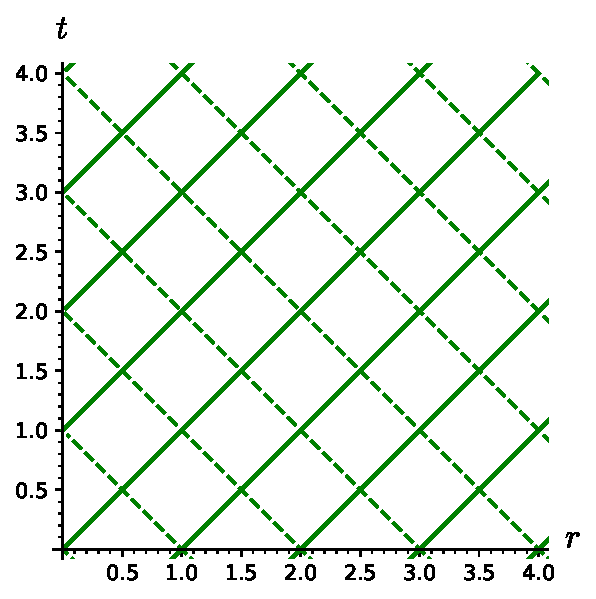
\includegraphics[width=0.5\textwidth]{glo_null_coord.pdf}}
\caption[]{\label{f:glo:null_coord} \footnotesize
Lines of constant null coordinates $u$ (solid) and $v$
(dashed) in terms of the coordinates $(t,r)$.}
\end{figure}


Let us introduce the null coordinate system $(u,v,\th,\ph)$ where $u$ and
$v$ are respectively the retarded\index{retarded!time} and advanced\index{advanced!time}
time defined by (cf. Fig.~\ref{f:glo:null_coord})
\be \label{e:glo:advanced_retarded}
    \left\{ \begin{array}{l}
    u = t - r\\
    v = t + r
    \end{array} \right.
    \iff
    \left\{ \begin{array}{l}
    t = \frac{1}{2} (v+u)\\[1ex]
    r = \frac{1}{2} (v-u) .
    \end{array} \right.
\ee
The metric tensor takes then the shape
\be \label{e:glo:Mink_metric_uv}
    \w{g} = - \dd u \, \dd v
        + \frac{1}{4} (v-u)^2 \left(  \dd\th^2 + \sin^2\th \, \dd\ph^2 \right) .
\ee
The coordinates $(u,v)$ span the half part of $\mathbb{R}^2$ defined by
$u<v$. In order to have coordinates within a finite range, let us consider
their arctangents (cf. Fig.~\ref{f:glo:atan}):
\be \label{e:glo:UV_uv}
    \left\{ \begin{array}{l}
    U = \arctan u \\
    V = \arctan v
    \end{array} \right.
    \iff
   \left\{ \begin{array}{l}
    u = \tan U \\
    v = \tan V .
    \end{array} \right.
\ee
Then the coordinates $(U,V)$ span the half part of $(-\pi/2, \pi/2)\times (-\pi/2, \pi/2)$
defined by $U < V$
(since $\arctan$ is a monotonically increasing function, cf. Fig.~\ref{f:glo:atan}):
\be \label{e:glo:span_UV}
    -\frac{\pi}{2} < U < \frac{\pi}{2}, \quad
    -\frac{\pi}{2} < V < \frac{\pi}{2}, \quad\mbox{and}\quad U < V.
\ee

\begin{figure}
\centerline{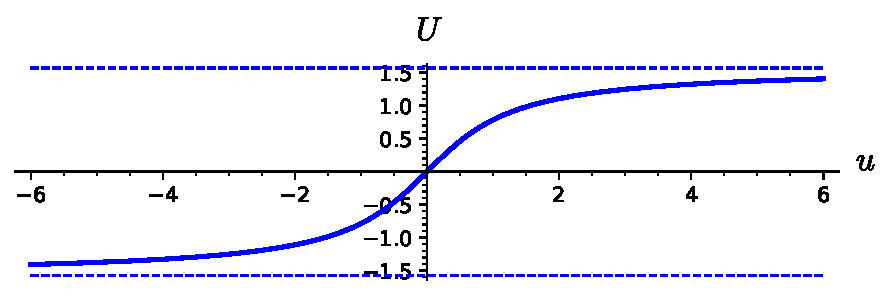
\includegraphics[width=0.8\textwidth]{glo_atan.pdf}}
\caption[]{\label{f:glo:atan} \footnotesize
The arctangent function mapping $\mathbb{R}$ to $(-\pi/2, \pi/2)$.}
\end{figure}

Since
\[
    \D u = \frac{\D U}{\cos^2 U}, \quad \D v = \frac{\D V}{\cos^2 V}
    \quad\mbox{and}\quad
    \tan V - \tan U = \frac{\sin(V-U)}{\cos U \cos V},
\]
the Minkowski metric (\ref{e:glo:Mink_metric_uv})
is expressed in terms of the coordinates $(U,V,\th,\ph)$
as\footnote{See also the SageMath notebook~\ref{s:sam:conformal_Mink}.}
\be \label{e:glo:g_UV}
    \w{g} = \frac{1}{4\cos^2 U \cos^2 V}
    \left[ - 4 \, \dd U \, \dd V + \sin^2(V-U) \left(  \dd\th^2 + \sin^2\th \, \dd\ph^2 \right)
    \right] .
\ee

\begin{remark}
The retarded/advanced times $u$ and $v$ have the dimension of a time, or of a
length in the $c=1$ units that we are using. Therefore, one should introduce
some length scale, $\ell_0$ say, before taking their arctangent and rewrite
(\ref{e:glo:UV_uv}) as
\[
    \left\{ \begin{array}{l}
    U = \arctan (u/\ell_0) \\
    V = \arctan (v/\ell_0)
    \end{array} \right.
    \iff
   \left\{ \begin{array}{l}
    u = \ell_0 \tan U \\
    v = \ell_0 \tan V .
    \end{array} \right.
\]
The coordinates $(U,V)$ are dimensionless and a global factor $\ell_0^2$ should be
introduced in the right-hand side of Eq.~(\ref{e:glo:g_UV}).
However, the length scale $\ell_0$ plays no essential role,
so that, to keep simple notations,
it is omitted in what follows. In other words, we are using units for
which $\ell_0=1$.
\end{remark}

\subsection{Conformal metric} \label{s:glo:conf_metric}

In the right-hand side of (\ref{e:glo:g_UV}),
the terms in square brackets defines a metric
$\w{\tilde{g}}$ such that
\be \label{e:glo:tilde_g_Omega}
    \encadre{ \w{\tilde{g}} = \Omega^2 \w{g} } ,
\ee
where $\Omega$ is the scalar field $\M \rightarrow \mathbb{R}$ obeying
\begin{subequations}
\begin{align}
    \Omega & =  2 \cos U \cos V \label{e:glo:Omega_UV} \\
           & =  \frac{2}{\sqrt{1+u^2}\sqrt{1+v^2}} \label{e:glo:Omega_uv}\\
           & =  \frac{2}{\sqrt{(t-r)^2+1}\sqrt{(t+r)^2+1}} . \label{e:glo:Omega_tr}
\end{align}
\end{subequations}
We notice on (\ref{e:glo:Omega_uv}) and (\ref{e:glo:Omega_tr}) that the function
$\Omega$ never vanishes on $\M$, so that the bilinear form $\w{\tilde{g}}$ defined by
(\ref{e:glo:tilde_g_Omega}) constitutes a well-behaved metric on $\M$.
Moreover, since $\Omega^2 > 0$, $\w{\tilde{g}}$ has the same signature as
$\w{g}$, i.e. $(-,+,+,+)$.
The specific expression of $\w{\tilde{g}}$ is deduced from (\ref{e:glo:g_UV})
and (\ref{e:glo:Omega_UV}):
\be \label{e:glo:tg_UV}
    \w{\tilde{g}} =  - 4 \, \dd U \, \dd V
        + \sin^2(V-U) \left(  \dd\th^2 + \sin^2\th \, \dd\ph^2 \right) .
\ee

In view of (\ref{e:glo:tilde_g_Omega}), one says that the metric $\w{\tilde{g}}$
is \defin{conformal to}\index{conformal} the metric $\w{g}$, or equivalently,
that the metrics $\w{g}$ and $\w{\tilde{g}}$ are
\defin{conformally related}\index{conformally related metrics},
or that $\w{\tilde{g}}$ arises from $\w{g}$ via a
\defin{conformal transformation}\index{conformal!transformation}.
The scalar field $\Omega$ is called the \defin{conformal factor}\index{conformal!factor}.

A key property of a conformal transformation is to preserve orthogonality
relations, since (\ref{e:glo:tilde_g_Omega}) clearly
implies, at any point $p\in\M$,
\[
    \forall (\w{u},\w{v})\in T_p\M\times T_p\M,\quad
    \w{\tilde{g}}(\w{u},\w{v}) = 0 \iff \w{g}(\w{u},\w{v}) = 0 .
\]
In particular, null vectors for $\w{\tilde{g}}$ coincide with null vectors for $\w{g}$:
\[
    \forall \wl \in T_p\M,\quad
    \w{\tilde{g}}(\wl,\wl) = 0 \iff \w{g}(\wl,\wl) = 0 .
\]
Consequently the light cones of $(\M,\w{g})$ and $(\M,\w{\tilde{g}})$
are identical, which implies that $(\M,\w{g})$ and $(\M,\w{\tilde{g}})$
have the same causal structure.
Moreover, since $\Omega^2>0$, the spacelike and timelike characters of vectors
is preserved as well:
\be
    \begin{array}{ll}
    \forall \w{v} \in T_p\M,\ &
        \w{v} \mbox{\ spacelike for\ } \w{\tilde{g}} \iff \w{v} \mbox{\ spacelike for\ } \w{g} \\
    & \w{v} \mbox{\ timelike for\ } \w{\tilde{g}} \iff \w{v} \mbox{\ timelike for\ } \w{g} .
    \end{array}
\ee
It follows that a curve $\Li$ is timelike (resp. null, spacelike) for $\w{\tilde{g}}$
iff $\Li$ is timelike (resp. null, spacelike) for $\w{g}$. Similarly,
a hypersurface $\Sigma$ is timelike (resp. null, spacelike) for $\w{\tilde{g}}$
iff $\Sigma$ is timelike (resp. null, spacelike) for $\w{g}$.

What about geodesics? Let us first recall that a null curve is not necessarily
a null geodesic (cf. Remark~\ref{r:def:null_curves} on page~\pageref{r:def:null_curves}
and Appendix~\ref{s:geo}),
so that one cannot deduce from the above results that conformal transformations
preserve null geodesics. However, this turns out to be true:
\begin{prop}[null geodesics preserved by conformal transformations]
A smooth curve $\Li$ in $\M$ is a null geodesic for $\w{\tilde{g}}$ iff
$\Li$ is a null geodesic for $\w{g}$.
\end{prop}
To prove it, it suffices to write explicitly the geodesic equation [Eq.~(\ref{e:geo:eq_geod})]
and to express the Christoffel symbols of $\w{\tilde{g}}$ in terms of those
of $\w{g}$ and the derivatives of $\Omega$ (see e.g. Appendix~D of Wald's
textbook \cite{Wald84} for details).

On the contrary, conformal transformations preserve neither timelike
geodesics nor spacelike ones.

The coordinates $(U,V)$ are of null type; let us consider instead
the ``time+space'' coordinates $(\tau,\chi)$ defined by\footnote{Notice the
similarity with (\ref{e:glo:advanced_retarded}) up to some $1/2$ factors.}
\be \label{e:glo:tau_chi_U_V}
    \left\{ \begin{array}{l}
    \tau = V + U \\
    \chi = V - U
    \end{array} \right.
    \iff
    \left\{ \begin{array}{l}
    U = \frac{1}{2} (\tau - \chi) \\[1ex]
    V = \frac{1}{2} (\tau + \chi) .
    \end{array} \right.
\ee
Given (\ref{e:glo:span_UV}), the range of these new coordinates is
\be \label{e:glo:range_tau_chi}
    0 < \chi < \pi \quad\mbox{and}\quad
    \chi - \pi < \tau < \pi - \chi .
\ee
In other words, if we draw the Minkowski spacetime in the $(\tau,\chi)$ plane,
it takes the shape of a half-diamond, as depicted in Fig.~\ref{f:glo:conf_diag_Mink}.

\begin{figure}
\centerline{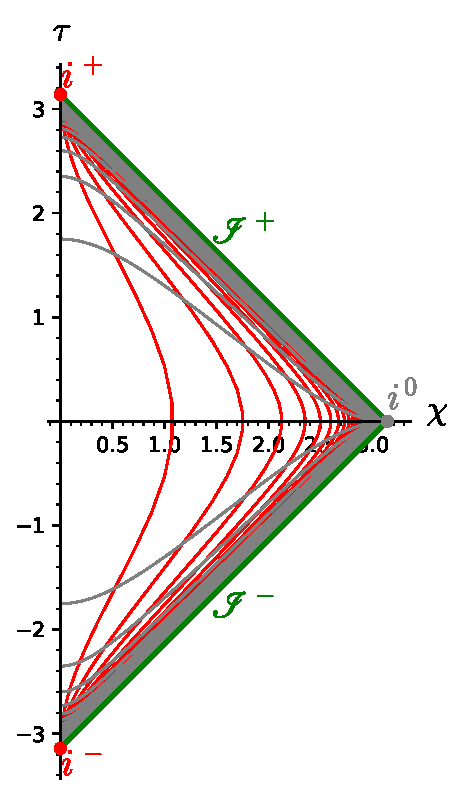
\includegraphics[width=0.35\textwidth]{glo_conf_diag_Mink.pdf}}
\caption[]{\label{f:glo:conf_diag_Mink} \footnotesize
Conformal diagram of Minkowski spacetime. Constant-$r$ curves are drawn in
red, while constant-$t$ ones are drawn in grey.
\textsl{[Figure generated by the notebook \ref{s:sam:conformal_Mink}]}
}
\end{figure}

By combining (\ref{e:glo:advanced_retarded}) (\ref{e:glo:UV_uv}) and
(\ref{e:glo:tau_chi_U_V}), we get the link between $(t,r)$ and
$(\tau,\chi)$:
\be \label{e:glo:tau_chi_t_r}
    \left\{ \begin{array}{l}
    \tau = \arctan(t+r) + \arctan(t-r) \\
    \chi = \arctan(t+r) - \arctan(t-r)
    \end{array} \right.
    \iff
    \left\{ \begin{array}{l}
    \displaystyle t = \frac{\sin\tau}{\cos\tau + \cos\chi}\\[2ex]
    \displaystyle r = \frac{\sin\chi}{\cos\tau + \cos\chi} .
    \end{array} \right.
\ee
We may use these relations to draw the lines $t=\mathrm{const}$ and
$r=\mathrm{const}$ in Fig.~\ref{f:glo:conf_diag_Mink}.

The expression of the conformal factor in the
coordinates $(\tau,\chi,\th,\ph)$ is easily deduced from
(\ref{e:glo:Omega_UV}) and
(\ref{e:glo:tau_chi_U_V}):
\be \label{e:glo:Omega_tau_chi}
    \Omega = \cos\tau + \cos\chi .
\ee


\subsection{Conformal completion} \label{s:glo:conf_complet_Mink}

The expression of the conformal metric in terms of the coordinates
$(\tau,\chi,\th,\ph)$ is easily deduced from that in terms of
$(U,V,\th,\ph)$ as given by (\ref{e:glo:tg_UV}):
\be \label{e:glo:tg_Einstein}
    \w{\tilde{g}} =  - \dd\tau^2
        + \dd \chi^2
        + \sin^2\chi \left(  \dd\th^2 + \sin^2\th \, \dd\ph^2 \right) .
\ee
Restricting to a $\tau = \mathrm{const}$ hypersurface, i.e. setting $\dd\tau=0$,
we recognize the standard metric of the hypersphere
$\mathbb{S}^3$ in the hyperspherical coordinates $(\chi,\th,\ph)$.
Moreover, we notice that the full metric (\ref{e:glo:tg_Einstein})
is perfectly regular even if we relax
the condition on $\tau$ in (\ref{e:glo:range_tau_chi}), i.e. if we
let $\tau$ span the
entire $\mathbb{R}$. We may then consider the manifold
\be
    \mathscr{E} = \mathbb{R}\times \mathbb{S}^3
\ee
and $\w{\tilde{g}}$ as the Lorentzian metric on $\mathscr{E}$ given by
(\ref{e:glo:tg_Einstein}).
The Lorentzian manifold
$(\mathscr{E},\w{\tilde{g}})$ is nothing but the
\defin{Einstein static universe}\index{Einstein!static universe}\index{static!universe (Einstein)}, also called the \defin{Einstein cylinder}\index{Einstein!cylinder}\index{cylinder!Einstein --},
a static solution of the Einstein equation (\ref{e:fra:Einstein_eq})
with $\Lambda > 0$ and some pressureless matter of uniform density
$\rho = \Lambda/(4\pi)$.
We have thus an embedding\footnote{Cf. Sec.~\ref{s:bas:embed} of Appendix~A} of Minkowski spacetime into the Einstein cylinder:
\be \label{e:glo:embed_Mink_Einst}
     \Phi:\ \M \longrightarrow \mathscr{E}
\ee
and this embedding is a conformal isometry from
$(\M,\w{g})$ to $(\Phi(\M),\w{\tilde{g}})$.
In the following, we shall identify $\Phi(\M)$ and $\M$, i.e. use the same
symbol $\M$ to denote the subset of $\mathscr{E}$ that is the image of $\M$ via the
embedding (\ref{e:glo:embed_Mink_Einst}).

\begin{figure}
\centerline{\includegraphics[width=0.6\textwidth]{glo_Einstcyl_Mink.pdf}}
\caption[]{\label{f:glo:Einstcyl_Mink}\footnotesize
Two views of the Einstein cylinder $\mathscr{E}$, with the conformal embedding of
Minkowski spacetime in it. Due to the dimensional reduction $4 \to 2$ for
the drawing, the
$\mathbb{S}^3$ sections of the cylinder are depicted as horizontal circles.
The red curves are the same constant-$r$ curves
as in Fig.~\ref{f:glo:conf_diag_Mink}, while the black curves are
the same constant-$t$ curves as those drawn in grey in Fig.~\ref{f:glo:conf_diag_Mink}.
\textsl{[Figure generated by the notebook \ref{s:sam:conformal_Mink}]}
}
\end{figure}

Since $\mathscr{E}$ and $\M$ have the same dimension, $\M$ is an open subset of $\mathscr{E}$.
Its closure $\overline{\M}$ in $\mathscr{E}$ is (cf.
Figs.~\ref{f:glo:conf_diag_Mink} and \ref{f:glo:Einstcyl_Mink})
\be
    \overline{\M} = \M \cup \scri^+ \cup \scri^- \cup \left\{ i^0 \right\} \cup
            \left\{ i^+ \right\} \cup \left\{ i^- \right\} ,
\ee
where
\begin{itemize}
\item $\scri^+$ is the hypersurface of $\mathscr{E}$ defined by
$\tau = \pi - \chi$ and $0 < \tau < \pi$;
\item $\scri^-$ is the hypersurface of $\mathscr{E}$ defined by
$\tau = \chi - \pi $ and $-\pi  < \tau < 0$;
\item $i^0$ is the point of $\mathscr{E}$ defined by $\tau=0$ and $\chi=\pi$;
\item $i^+$ is the point of $\mathscr{E}$ defined by $\tau=\pi$ and $\chi=0$;
\item $i^-$ is the point of $\mathscr{E}$ defined by $\tau=-\pi$ and $\chi=0$.
\end{itemize}
It is customary to pronounce $\scri$ as ``scri'', for \emph{script i}.

\begin{remark}
On $\mathbb{S}^3$, the hyperspherical coordinates $(\chi,\th,\ph)$
are singular at $\chi=0$ and $\chi=\pi$, so that setting $\chi=0$ (or $\chi=\pi$)
defines a unique point of $\mathbb{S}^3$, whatever the value of $(\th,\ph)$.
Note also that the vertical left boundary of the diamond drawn in
Fig.~\ref{f:glo:conf_diag_Mink}, i.e. the segment defined by
$\tau\in(-\pi,\pi)$ and $\chi=0$, is \emph{not} a part of the boundary
of $\M$ but merely reflect the coordinate singularity at $\chi=0$, in the same
way that the left vertical boundary of Fig.~\ref{f:glo:null_coord}
is not a boundary of Minkowski spacetime but is
due to the coordinate singularity at $r=0$. Note by the way that
$\chi=0$ implies $r=0$ via (\ref{e:glo:tau_chi_t_r}).
\end{remark}

Let
\be
    \scri := \scri^+ \cup \scri^-
\ee
and
\be \label{e:glo:def_tM_Mink}
    \tilde{\M} := \M \cup \scri .
\ee
$\tilde{\M}$ is naturally a smooth manifold with
boundary\footnote{Cf. Sec.~\ref{s:bas:manif_boundary} for the precise definition.}\index{manifold!with boundary}
and its boundary is $\scri$:
\be
    \partial \tilde{\M} = \scri.
\ee
\begin{remark}
Because the closure $\overline{\M}$ is self-intersecting at the point $i^0$
(cf. Fig.~\ref{f:glo:Einstcyl_Mink}), it is not a manifold with boundary: no open neighbourhood of
$i^0$ is homeomorphic to a neighbourhood of
$\mathbb{H}^4 = \mathbb{R}^3\times {[0,+\infty)}$,
as the definition of a manifold with boundary would
require, cf. Sec.~\ref{s:bas:manif_boundary}.
At the points $i^+$ and $i^-$, $\overline{\M}$ can be considered as a
topological manifold with boundary, but not as a \emph{smooth} manifold with boundary.
Hence, the three points $i^0$, $i^+$ and $i^-$ are excluded from the definition
of the manifold with boundary $\tilde{\M}$.
\end{remark}

\begin{figure}
\centerline{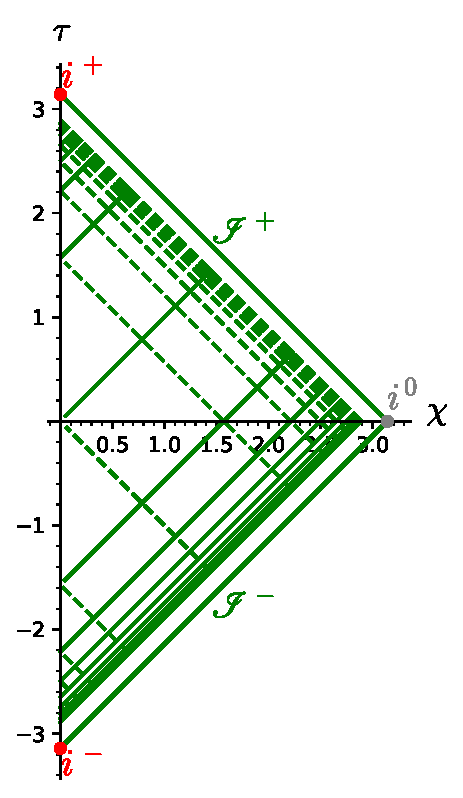
\includegraphics[width=0.35\textwidth]{glo_conf_Mink_null.pdf}}
\caption[]{\label{f:glo:conf_Mink_null}\footnotesize
Null radial geodesics in the conformal diagram of Minkowski spacetime.
The solid green lines are null geodesics $u=\mathrm{const}$ for
17 values of $u$ uniformly spanning $[-8,8]$, while the dashed green lines are
null geodesics $v=\mathrm{const}$ for 17 values of $v$ uniformly spanning $[-8,8]$.
\textsl{[Figure generated by the notebook \ref{s:sam:conformal_Mink}]}
}
\end{figure}

The hypersurface $\scri^+$ is the location of $\tilde{\M}$ where all radial null geodesics
terminate, while $\scri^-$ is the location of $\tilde{\M}$ where all these geodesics originate (cf. Fig.~\ref{f:glo:conf_Mink_null}). For this
reason $\scri^+$ is called the
\defin{future null infinity}\index{future!null infinity}\index{null!infinity}
of $(\M,\w{g})$
and $\scri^-$ the \defin{past null infinity}\index{past!null infinity}
of $(\M,\w{g})$.
On the other side, any timelike geodesic of $(\M,\w{g})$ originates at $i^-$ and ends at
$i^+$ (cf. Fig.~\ref{f:glo:conf_diag_Mink}), while any spacelike geodesic
of $(\M,\w{g})$ originates at $i^0$ and terminates there
(after having completed a closed path on $\mathbb{S}^3$ (cf. Fig.~\ref{f:glo:Einstcyl_Mink}).
The point $i^+$ is then called the
\defin{future timelike infinity}\index{future!timelike infinity}\index{timelike!infinity}
of $(\M,\w{g})$,
$i^-$ the \defin{past timelike infinity}\index{past!timelike infinity}
of $(\M,\w{g})$
and $i^0$ the \defin{spacelike infinity}\index{spacelike!infinity} of $(\M,\w{g})$.

As it is clear on the conformal diagram of Fig.~\ref{f:glo:conf_diag_Mink},
both $\scri^+$ and $\scri^-$ are null hypersurfaces of $(\tilde{\M},\w{\tilde{g}})$.

\begin{figure}
\centerline{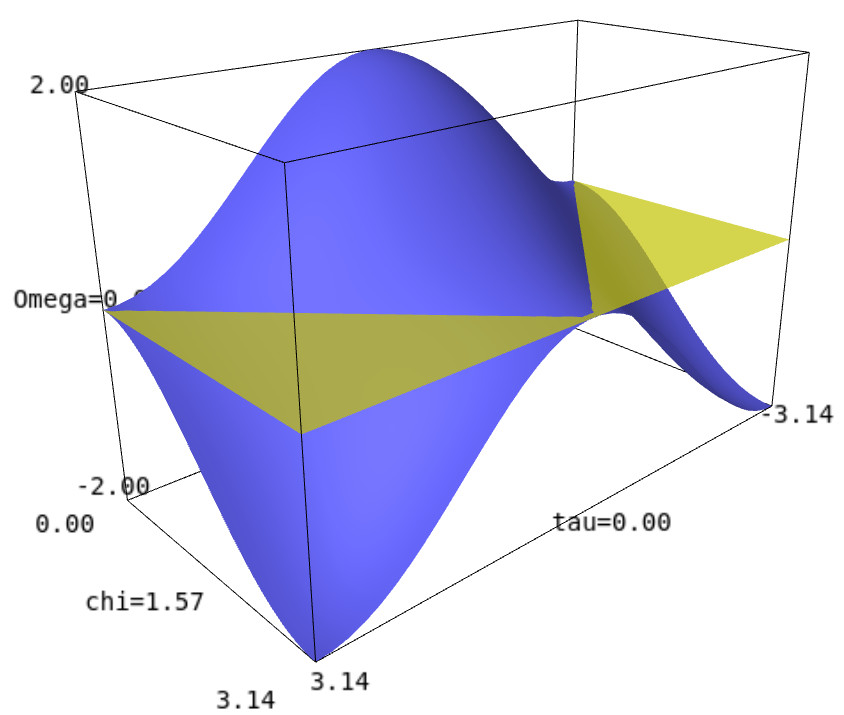
\includegraphics[width=0.45\textwidth]{glo_Omega_Mink.jpg}}
\caption[]{\label{f:glo:Omega_Mink}\footnotesize
Conformal factor $\Omega$ as a function of $(\tau,\chi)$ [cf. Eq.~(\ref{e:glo:Omega_tau_chi})].
Only the part above the yellow horizontal plane ($\Omega=0$) is physical.
\textsl{[Figure generated by the notebook \ref{s:sam:conformal_Mink}]}
}
\end{figure}


It is precisely because $\Omega$ vanishes (cf. Fig.~\ref{f:glo:Omega_Mink}) at the boundary
\be
    \overline{\M} \setminus \M = \scri^+ \cup \scri^- \cup \left\{ i^0 \right\} \cup
            \left\{ i^+ \right\} \cup \left\{ i^- \right\}
\ee
that the conformal transformation (\ref{e:glo:tilde_g_Omega}) brings infinity
of Minkowski space to a finite distance.

\begin{hist}
The idea of using a conformal transformation to treat infinity as a boundary
``at a finite distance'' has been put forward by Roger Penrose\index[pers]{Penrose, R.}
in 1963 \cite{Penro63} and expanded in 1964 in the seminal paper \cite{Penro64},
where Penrose constructed the
conformal completion of Minkowski spacetime as a part of the Einstein cylinder.
In particular, Fig.~3 of Ref.~\cite{Penro64} is equivalent to Fig.~\ref{f:glo:Einstcyl_Mink}.
\end{hist}


%%%%%%%%%%%%%%%%%%%%%%%%%%%%%%%%%%%%%%%%%%%%%%%%%%%%%%%%%%%%%%%%%%%%%%%%%%%%%%%%%%%%%%%%

\section{Conformal completions and asymptotic flatness} \label{s:glo:conf_compl}

Having investigated the asymptotic structure of Minkowski spacetime
via a conformal completion, let us use the latter to define spacetimes
that ``look like'' Minkowski spacetime asymptotically.
A first step is the concept of conformal completion.

\subsection{Conformal completion} \label{s:glo:def_conf_compl}

\begin{greybox}
A spacetime $(\M,\w{g})$ admits a
\defin{conformal completion}\index{conformal!completion}
iff there exists a Lorentzian manifold with boundary
$(\tilde{\M},\w{\tilde{g}})$ equipped with a smooth non-negative scalar field
$\Omega: \tilde{\M} \rightarrow \mathbb{R}^+$
such that
\begin{enumerate}
\item $\tilde{\M} = \M \cup \scri$, with $\scri := \partial \tilde{\M}$
(the boundary of $\tilde{\M})$;
\item on $\M$, $\w{\tilde{g}} = \Omega^2 \w{g}$;
\item on $\scri$, $\Omega=0$;
\item on $\scri$, $\dd \Omega \not= 0$.
\end{enumerate}
$\scri$ is called the \defin{conformal boundary}\index{conformal!boundary}\index{boundary!conformal --}
of $(\M,\w{g})$ within
the conformal completion $(\tilde{\M},\w{\tilde{g}})$.
\end{greybox}
Condition~1 expresses that $\M$ has been endowed with some boundary.
A rigorous formulation of it would be via an embedding $\Phi:\M \rightarrow \tilde{\M}$,
as in Eq.~(\ref{e:glo:embed_Mink_Einst}), so that
$\tilde{\M} = \Phi(\M) \cup \scri$. However, as above, we identify $\Phi(\M)$
with $\M$ and therefore simply write $\tilde{\M} = \M \cup \scri$.
Conditions~2 and 3 express that the boundary of $\M$, which ``lies at an infinite
distance'' with respect to $\w{g}$, has been brought to a
finite distance with respect to $\w{\tilde{g}}$. Indeed, in terms of
length elements [cf. Eq.~(\ref{e:fra:line_element})], condition~2 implies
\[
    \D s^2 = \frac{1}{\Omega^2} \, \D {\tilde s}^2
\]
with $1/\Omega^2 \rightarrow +\infty$ as one approaches $\scri$
(condition~3).
Finally, condition~4 ensures
that $\scri$ is a regular hypersurface of $\tilde{\M}$.
It is of course fulfilled by Minkowski spacetime, as we can check graphically
on Fig.~\ref{f:glo:Omega_Mink}: the graph of $\Omega$ has no horizontal slope
at $\scri$.

\begin{remark}
The statement that $(\tilde{\M},\w{\tilde{g}})$ is a Lorentzian manifold with
boundary implies that $\w{\tilde{g}}$ is smooth everywhere on $\tilde{\M}$,
including at the boundary $\scri$.
\end{remark}

\begin{remark}
The conformal boundary $\scri$ is not part of the physical spacetime
$\M$, but only of the conformal completion $\tilde{\M}$.
\end{remark}

\begin{remark}
One often speaks about
\emph{conformal compactification}\index{conformal!compactification}\index{compactification}
instead of \emph{conformal completion}, but in general $\tilde{\M}$ is not a
compact manifold. For instance, because we omitted the points $i^+$, $i^-$ and $i^0$,
the completion $\tilde{\M}$ of Minkowski spacetime defined by Eq.~(\ref{e:glo:def_tM_Mink})
is not compact.
\end{remark}

\begin{figure}
\centerline{\includegraphics[height=0.4\textheight]{glo_AdS_completion.pdf}}
\caption[]{\label{f:glo:AdS_completion} \footnotesize
Conformal completion of AdS$_{4}$ spacetime, depicted on the Einstein cylinder.
The conformal boundary $\scri$ is shown in yellow, red lines are lines
$\chi=\mathrm{const}$ (uniformly sampled in terms of $\tan\chi = \sinh\rho$),
green curves are radial null geodesics and the purple curve
is a radial timelike geodesic, bouncing back and forth around $\chi=0$.
\textsl{[Figure generated by the notebook \ref{s:sam:AdS}]}
}
\end{figure}

\begin{example}[conformal completion of AdS$_{4}$ spacetime] \label{x:glo:AdS}
The 4-dimensional anti-de Sitter spacetime\index{anti-de Sitter spacetime}
$(\M,\w{g})$
has been introduced in Example~\ref{x:neh:AdS} of Chap.~\ref{s:neh}.
The metric tensor expressed in the conformal coordinates
$(\tau,\chi,\th,\ph)$ is given by Eq.~(\ref{e:neh:metrix_AdS_conformal}):
\be
    \w{g} = \frac{\ell^2}{\cos^2\chi} \left[ - \dd \tau^2
    + \dd \chi^2 + \sin^2\chi \left( \dd\th^2 + \sin^2\th \, \dd\ph^2 \right) \right] ,
\ee
with $\tau\in\R$, $\chi \in (0,\pi/2)$, $\th\in(0,\pi)$ and $\ph\in(0,2\pi)$.
Defining $\Omega := \ell^{-1}\cos\chi$, we notice that
a conformal completion of $(\M,\w{g})$ is $(\tilde{\M},\w{\tilde{g}})$
where (i) $\tilde{\M}$ is the part $\chi \leq \pi/2$ of the Einstein cylinder\footnote{Recall that on the
Einstein cylinder the range of $\chi$ is $(0,\pi)$, cf. Eq.~(\ref{e:glo:range_tau_chi}).}
introduced in Sec.~\ref{s:glo:conf_complet_Mink}
and (ii)  $\w{\tilde{g}}$ is the metric (\ref{e:glo:tg_Einstein}).
The boundary $\scri = \partial\tilde{\M}$ is then the hypersurface $\chi=\pi/2$
of the Einstein cylinder (cf. Fig.~\ref{f:glo:AdS_completion});
$\scri$ is spanned by the coordinates $(\tau,\th,\ph)$
and its topology is that of a 3-dimensional cylinder: $\scri \simeq \mathbb{R}\times\mathbb{S}^2$.
We notice that conditions 3 and 4 of the definition of a conformal completion
are satisfied: $\Omega = \ell^{-1} \cos\chi = 0$ at $\scri$ and
$\dd\Omega = - \ell^{-1} \sin\chi\, \dd\chi = -\ell^{-1} \dd\chi \not = 0 $
at $\scri$.
The metric induced by $\w{\tilde{g}}$ on $\scri$ is obtained by
setting $\chi=\pi/2$ in (\ref{e:glo:tg_Einstein}):
$- \dd \tau^2 + \dd\th^2 + \sin^2\th \, \dd\ph^2$.
This 3-metric is clearly Lorentzian, which shows that $\scri$ is a timelike
hypersurface of $(\tilde{\M},\w{\tilde{g}})$.
\end{example}

The above example shows that $\scri$ is not necessarily a null hypersurface,
as it is for Minkowski spacetime (cf. Sec.~\ref{s:glo:conf_complet_Mink}).
Actually the causal type of $\scri$ is determined by the cosmological
constant, as follows:
\begin{prop}[causal type of $\scri$ and sign of the cosmological constant]
\label{p:glo:type_scri_sign_Lambda}
If the spacetime dimension obeys\footnote{Cf. Remark~\ref{r:fra:Einstein_eq_n_2} in
Sec.~\ref{s:fra:Einstein_eq}.}
$n\geq 3$ and $\w{g}$ is a solution of Einstein equation with
a cosmological constant $\Lambda$ [Eq.~(\ref{e:fra:Einstein_eq})]
and the trace $T$ of the energy-momentum tensor tends to zero in the
vicinity of $\scri$ (i.e. when $\Omega\rightarrow 0$), then
\begin{itemize}
\item $\scri$ is a null hypersurface of $(\tilde{\M},\w{\tilde{g}})$ iff $\Lambda=0$;
\item $\scri$ is a spacelike hypersurface of $(\tilde{\M},\w{\tilde{g}})$ iff $\Lambda>0$;
\item $\scri$ is a timelike hypersurface of $(\tilde{\M},\w{\tilde{g}})$ iff $\Lambda<0$.
\end{itemize}
\end{prop}
\begin{proof}
It follows from $\w{\tilde{g}} = \Omega^2 \w{g}$ that the Ricci scalars $\tilde{R}$
and $R$ of respectively $\w{\tilde{g}}$ and $\w{g}$ are related by\footnote{This relation is
easily established by starting from Eq.~(2.30) of Hawking \& Ellis textbook~\cite{HawkiE73} or Eq.~(2.19) on page~645 of Choquet-Bruhat one~\cite{Choqu09} and inverting the roles of $\w{\tilde{g}}$ and $\w{g}$, thereby substituting
$\Omega^{-1}$ for $\Omega$.}
\be \label{e:glo:tildeR_R}
    \Omega^2 \tilde{R} = R - (n-1) \left( 2 \Omega \, \tilde{g}^{\mu\nu} \tilde{\nabla}_\mu
    \tilde{\nabla}_\nu \Omega - n \, \tilde{g}^{\mu\nu} \partial_\mu \Omega \partial_\nu \Omega
    \right) ,
\ee
where $n = \mathrm{dim}\, \M$ and $\tilde{\nabla}$ stands for the Levi-Civita connection of
$\w{\tilde{g}}$. Using the trace of the Einstein equation (\ref{e:fra:Einstein_eq_n}) to
express $R$, we get
\[
    \Omega^2 \tilde{R} = \frac{2}{n-2}\left( n \Lambda - 8\pi T \right)
     - (n-1) \left( 2 \Omega \, \tilde{g}^{\mu\nu} \tilde{\nabla}_\mu
    \tilde{\nabla}_\nu \Omega - n \, \tilde{g}^{\mu\nu} \partial_\mu \Omega \partial_\nu \Omega
    \right)
\]
This equation is a priori valid in $\M = \tilde{\M}\setminus\scri$ only.
Taking the limit $\Omega\rightarrow 0$ and
assuming that $T\rightarrow 0$ in that limit, we get, by continuity, an identity
on $\scri$:
\be \label{e:glo:normal_scri_square}
\tilde{g}^{\mu\nu} \partial_\mu \Omega \partial_\nu \Omega \stackrel{\scri}{=}
    - \frac{2}{(n-1)(n-2)} \Lambda .
\ee
Since $\scri$ corresponds to a constant value of the scalar field $\Omega$ ($\Omega=0$),
the left-hand side of this equation is nothing but the scalar square
$\w{\tilde{g}}(\w{n},\w{n})$ of the vector $\w{n}$ normal to $\scri$
defined as the dual with respect to $\w{\tilde{g}}$ of the 1-form
$\dd\Omega$: $n^\alpha = \tilde{g}^{\alpha\mu} \partial_\mu \Omega$
(remember that by hypothesis 4 in the definition
of a conformal completion, $\dd\Omega$ is non-vanishing on $\scri$, so that
$\w{n}$  is a valid normal
vector to $\scri$). Equation~(\ref{e:glo:normal_scri_square}) implies
that the sign of $\w{\tilde{g}}(\w{n},\w{n})$ is the opposite of that of $\Lambda$.
Given the link between the causal type of a hypersurface and the causal type of its normal
(cf. Sec.~\ref{s:def:hor_as_null}), this completes the proof.
\end{proof}

The definition of black hole shall involve a subcategory of conformal completions:

\begin{greybox}
Let $(\M,\w{g})$ be a time-orientable\footnote{Cf. Sec.~\ref{s:fra:time_orientation}.} spacetime admitting a conformal completion $(\tilde{\M},\w{\tilde{g}})$.
One says that $(\tilde{\M},\w{\tilde{g}})$ is a
\defin{conformal completion at null infinity}\index{conformal!completion!at null infinity}
of $(\M,\w{g})$
iff the boundary $\scri := \partial\tilde{\M}$ obeys
\be \label{e:glo:conf_comp_null_inf}
    \scri = \scri^+ \cup \scri^-,
\ee
with $\scri^+$ (resp. $\scri^-$) being never intersected by any past-directed
(resp. future-directed) causal
curve originating in $\M$. Let us recall that a
\defin{causal curve}\index{causal!curve} is
curve whose tangent vectors are nowhere spacelike.
As for Minkowksi spacetime, we shall call $\scri^+$ the
\defin{future null infinity}\index{future!null infinity}\index{null!infinity}
and $\scri^-$ the \defin{past null infinity}\index{past!null infinity}
of $(\M,\w{g})$.
\end{greybox}

\begin{remark}
The above definition of $\scri^+$ and $\scri^-$ does not impose
that these two objects are null hypersurfaces of $(\tilde{\M},\w{\tilde{g}})$.
This is true for Minkowski spacetime, but cannot hold for spacetimes with a
non-zero cosmological constant, as shown above. In particular, the following
example exhibits spacelike $\scri^+$ and $\scri^-$.
\end{remark}

\begin{example}[Conformal completion of dS$_{4}$ spacetime]
The 4-dimensional \defin{de Sitter spacetime}\index{de Sitter spacetime} is
$(\M,\w{g})$ with $\M\simeq \mathbb{R}\times\mathbb{S}^3$ and $\w{g}$ is the metric
whose expression in the so-called \emph{global coordinates}
$(t,\chi,\th,\ph)$ is
\be \label{e:glo:dS4}
    \w{g} = \ell^2 \left[ - \dd t^2
    + \cosh^2 t \left(
    \dd \chi^2 + \sin^2\chi \left( \dd\th^2 + \sin^2\th \, \dd \ph^2 \right) \right) \right] ,
\ee
where $\ell$ is a positive constant. Note that $t$ spans $\mathbb{R}$
while $(\chi,\th,\ph)$ are standard polar coordinates on $\mathbb{S}^3$:
$\chi\in(0,\pi)$, $\th\in(0,\pi)$ and $\ph\in(0,2\pi)$.
 The metric (\ref{e:glo:dS4}) is a solution
of the vacuum Einstein equation\index{Einstein!equation!vacuum --}\index{vacuum!Einstein equation} (\ref{e:fra:vac_Einstein_Lambda}) with
the positive cosmological constant $\Lambda = 3/\ell^2$.
Using coordinates $(\tau,\chi,\th,\ph)$ with
$\tau := 2\arctan(\tanh(t/2)) \in (-\pi/2,\pi/2)$, one gets
\be
    \w{g} = \frac{\ell^2}{\cos^2\tau} \left[ - \dd \tau^2
    + \dd \chi^2 + \sin^2\chi \left( \dd\th^2 + \sin^2\th \, \dd\ph^2 \right) \right] .
\ee
Defining $\Omega := \ell^{-1}\cos\tau = (\ell\cosh t)^{-1}$, we notice that
a conformal completion of $(\M,\w{g})$ is $(\tilde{\M},\w{\tilde{g}})$
where (i) $\tilde{\M}$ is the part $-\pi/2\leq \tau \leq \pi/2$ of the Einstein cylinder
introduced in Sec.~\ref{s:glo:conf_complet_Mink}
and (ii)  $\w{\tilde{g}}$ is the metric (\ref{e:glo:tg_Einstein}).
The boundary $\scri = \partial\tilde{\M}$ has two connected components:
$\scri^+$, which is the hypersurface $\tau = \pi/2$ of $\tilde{\M}$, and
$\scri^-$, which is the hypersurface $\tau = -\pi/2$.
Both $\scri^+$ and $\scri^-$ are spanned by the coordinates $(\chi,\th,\ph)$
and their topology is that of $\mathbb{S}^3$.
We notice that conditions 3 and 4 of the definition of a conformal completion
are satisfied: $\Omega = \ell^{-1} \cos\tau = 0$ at $\scri$ and
$\dd\Omega = - \ell^{-1} \sin\tau\, \dd\tau = \pm \ell^{-1} \dd\tau \not = 0 $
at $\scri$.
The metric induced by $\w{\tilde{g}}$ on $\scri$ is obtained by
setting $\tau=\pm\pi/2$ in (\ref{e:glo:tg_Einstein}):
$\dd \chi^2 + \sin^2\chi \left( \dd\th^2 + \sin^2\th \, \dd\ph^2 \right) $.
This 3-metric is clearly Riemannian (this is actually the standard round metric
of $\mathbb{S}^3$), which shows that $\scri$ is a spacelike
hypersurface of $(\tilde{\M},\w{\tilde{g}})$. This of course agrees with
Property~\ref{p:glo:type_scri_sign_Lambda}, given that $\Lambda > 0$.
Finally, it is clear that
any causal curve originating in $\M$ that intersects $\scri^+$ must approach
$\tau=\pi/2$ from below, i.e. cannot be past-directed. Similarly any
causal curve originating in $\M$ that intersects $\scri^-$ must approach
$\tau=-\pi/2$ from above, i.e. cannot be future-directed. We conclude
that $(\tilde{\M},\w{\tilde{g}})$ is a conformal completion at null infinity
of the de Sitter spacetime.
\end{example}

\subsection{Asymptotic flatness} \label{s:glo:asymp_flat}

Penrose\index[pers]{Penrose, R.} \cite{Penro64,Penro68} has defined
a spacetime $(\M,\w{g})$ to be \defin{asymptotically simple}\index{asymptotically!simple} iff there exists
a conformal completion $(\tilde{\M},\w{\tilde{g}})$
of $(\M,\w{g})$
such that every null geodesic in $\M$ has two endpoints in $\scri$.

The last condition, which is verified by Minkowski spacetime (cf. Fig.~\ref{f:glo:conf_Mink_null}),
de Sitter spacetime and anti-de Sitter spacetime (cf. the null geodesics in
Fig.~\ref{f:glo:AdS_completion}), is rather restrictive. In particular, it excludes
black hole spacetimes, since, almost by definition, the latter contain null
geodesics that have no endpoint on $\scri^+$, having only a past endpoint
on $\scri^-$, as far as $\scri$ is concerned. To cope with these spacetimes,
Penrose\index[pers]{Penrose, R.} has also introduced the following definition \cite{Penro68}:
a spacetime $(\M,\w{g})$ is
\defin{weakly asymptotically simple}\index{weakly!asymptotically simple} iff
there exists an open subset $\mathscr{U}$ of $\M$ and
an asymptotically simple spacetime $(\M_0, \w{g}_0)$
with an open neighbourhood $\mathscr{U}_0$ of $\scri_0 = \partial \tilde{\M}_0$
in $\tilde{\M}_0$ such that $(\mathscr{U}_0\cap \M_0,\w{g}_0)$ is
isometric to $(\mathscr{U},\w{g})$.

\begin{remark}
For a given weakly asymptotically simple spacetime, there may be different
(non overlapping) regions $\mathscr{U}$ satisfying the above property.
For instance we shall see in Chap.~\ref{s:ker}
that there are an infinite series of them in the Kerr spacetime.
\end{remark}

Finally one says that a spacetime $(\M,\w{g})$ is
\defin{asymptotically flat}\index{asymptotically!flat}\index{flat!asymptotically --}
(or more precisely \defin{weakly asymptotically simple and empty}\index{weakly!asymptotically simple and empty} \cite{HawkiE73})
iff $(\M,\w{g})$ is weakly asymptotically simple and the Ricci tensor of
$\w{g}$ vanishes in an open neighbourhood of $\scri$: $\w{R} = 0$.

\begin{example}
The de Sitter and anti-de Sitter spacetimes are asymptotically simple but
are not asymptotically flat.
\end{example}

Penrose \cite{Penro65b} (see also \cite{Fraue04}) has shown that if $(\M,\w{g})$
is asymptotically simple and empty, that the Weyl tensor of $\w{g}$ (cf. Sec.~\ref{s:bas:Weyl})
vanishes at $\scri$. Since the
Ricci tensor is zero, this implies that the full Riemann curvature tensor vanishes
at $\scri$ [cf. Eq.~(\ref{e:bas:Weyl})], hence the qualifier \emph{asymptotically flat}.

The following property holds:
\begin{prop}
The conformal boundary $\scri$ of an asymptotically flat spacetime $(\M,\w{g})$
is a null hypersurface of the conformal completion $(\tilde{\M},\w{\tilde{g}})$.
\end{prop}
\begin{proof}
Consider Eq.~(\ref{e:glo:tildeR_R}). Near $\scri$, we have $R=0$ by the
very definition of asymptotic flatness. The limit $\Omega\rightarrow 0$
results then in
$\tilde{g}^{\mu\nu} \partial_\mu \Omega \partial_\nu \Omega \stackrel{\scri}{=} 0$,
which, following the argument in the proof on p.~\pageref{e:glo:tildeR_R}, implies that
$\scri$ is a null hypersurface.
\end{proof}


%%%%%%%%%%%%%%%%%%%%%%%%%%%%%%%%%%%%%%%%%%%%%%%%%%%%%%%%%%%%%%%%%%%%%%%%%%%%%%%%%%%%%%%%

\section{Black holes} \label{s:glo:BH}

\subsection{Preliminaries regarding causal structure}  \label{s:glo:causal_struct}

Before we proceed to the precise definition of a black hole, let us introduce
some concepts regarding the causal structure of a given time-orientable spacetime $(\M,\w{g})$.
For any subset $S$ of $\M$, one defines
\begin{itemize}
\item the \defin{chronological future of $S$}\index{chronological!future} as the set $I^+(S)$ of all
points of $\M$ that can be reached from a point of $S$ by a future-directed
timelike curve of nonzero extent;
\item the \defin{causal future of $S$}\index{causal!future} as the set $J^+(S)$ of
all points that either are in $S$ or can be reached from a point of $S$ by a future-directed
causal curve;
\item the \defin{chronological past of $S$}\index{chronological!past} as the set $I^-(S)$ of all
points of $\M$ that can be reached from a point of $S$ by a past-directed
timelike curve of nonzero extent;
\item the \defin{causal past of $S$}\index{causal!past} as the set $J^-(S)$ of
all points that either are in $S$ or can be reached from a point of $S$ by a past-directed
causal curve.
\end{itemize}
From the above definitions, one has always $S \subset J^\pm(S)$ and
$I^\pm(S) \subset J^\pm(S)$.

\begin{remark}
One has not necessarily $S \subset I^\pm(S)$. For instance,
if the spacetime does not contain
any closed timelike curve, one has  $S \cap I^\pm(S) = \varnothing$ for
$S = \{p\}$ with $p$ any point of $\M$.
\end{remark}

Here are some basic topological properties of the future and past sets
defined above (see e.g. \S~6.2 of \cite{HawkiE73} or Chap.~14 of
\cite{ONeil83} for proofs):
\begin{itemize}
\item
$I^\pm(S)$ is always an open subset\footnote{This property is a direct
consequence of Lemma~\ref{p:glo:lem1} in Sec.~\ref{s:glo:properties_H} below.} of $\M$, while
$J^\pm(S)$ is not necessarily a closed subset.
\item The interior of $J^\pm(S)$ is $I^\pm(S)$:
\be \label{e:glo:int_JS_IS}
    \mathrm{int}\, J^\pm(S) = I^\pm(S).
\ee
\item Both sets have the same closure:
\be \label{e:glo:clos_JS_IS}
    \overline{J^\pm(S)} = \overline{I^\pm(S)} .
\ee
\item
It follows from (\ref{e:glo:int_JS_IS}) and (\ref{e:glo:clos_JS_IS})
that both sets share the same boundary:
\be \label{e:glo:boundary_JS_IS}
    \partial J^\pm(S) = \partial I^\pm(S).
\ee
\end{itemize}

\subsection{General definition of a black hole} \label{s:glo:def_BH}

We are now in position to give the general definition of a black hole.
We shall do it for a spacetime $(\M,\w{g})$ that admits a conformal completion
at null infinity as defined in Sec.~\ref{s:glo:conf_compl} and thus
possesses a future null infinity $\scri^+$.
Moreover, we shall assume that $\scri^+$ is \defin{complete}\index{complete!future null infinity}: if $\scri^+$
is a null hypersurface, which occurs if $(\M,\w{g})$ is asymptotically flat
(cf. Sec.~\ref{s:glo:asymp_flat}),
this means that $\scri^+$ is generated by complete\footnote{Let us recall
that a \emph{complete} geodesic is an inextendible (i.e. maximal) geodesic,
whose affine parameters range through the whole of $\R$, cf. Sec.~\ref{s:geo:existence_uniqueness}
in Appendix~\ref{s:geo}.} null geodesics.
The completeness condition is imposed to avoid ``spurious'' black holes,
such as black holes in Minkowski space (cf. Remark~\ref{s:glo:spurious_bh} below).
The neighbourhood of $\scri^+$
in $\tilde{\M}$ can then be considered as the infinitely far region
reached by outgoing null geodesics. If a null geodesic does not reach this
region, it can be considered as being trapped somewhere else in spacetime: this
``somewhere else'' constitutes the black hole region.

\begin{greybox}
Let $(\M,\w{g})$ be a spacetime with a conformal completion at null infinity
such that $\scri^+$ is complete;
the \defin{black hole region}\index{black hole!region}, or simply \defin{black hole}\index{black hole},
is the set of points of $\M$ that are not in the causal past of the future null infinity:
\be \label{e:glo:def_BH}
    \encadre{\mathscr{B} := \M \setminus (J^-(\scri^+)\cap\M) } .
\ee
(cf. Fig.~\ref{f:glo:def_bh}).
\end{greybox}
The black hole region is thus the set of points of $\M$
from which no future-directed causal curve in $\tilde{\M}$ reaches $\scri^+$.
Of course, it may be that $\mathscr{B} = \varnothing$, in which case one
says that the spacetime $(\M,\w{g})$ contains no black hole.


\begin{figure}
\centerline{\includegraphics[width=0.6\textwidth]{glo_def_bh.pdf}}
\caption[]{\label{f:glo:def_bh} \footnotesize
The black hole region $\mathscr{B}$ defined as the complement of
the causal past of the future null infinity, $J^-(\scri^+)$.}
\end{figure}


\begin{example}
The Minkowski spacetime contains no black hole, for all future-directed null geodesics
terminate at $\scri^+$ (cf. Fig.~\ref{f:glo:conf_Mink_null}).
More generally, any asymptotically simple spacetime contains no black hole.
\end{example}

\begin{example}
The prototype of a black hole is the \emph{Schwarzschild black hole}; it will
be shown in Sec.~\ref{s:sch:BH} that the Schwarzschild spacetime contains
a region $\mathscr{B}$ that fulfills the above definition of a black hole.
The corresponding event horizon is nothing but the
Schwarzschild horizon\index{Schwarzschild!horizon} considered in the examples
of Chaps.~\ref{s:def} and \ref{s:neh}.
\end{example}

\begin{remark} \label{s:glo:spurious_bh}
If we release the assumption of $\scri^+$-completeness in the above definition,
we may end up with unphysical or ``spurious'' black holes.
For instance, let us consider the conformal completion of Minkowski spacetime
$(\M,\w{g})$ resulting from its embedding in the Einstein cylinder
$(\E,\w{\tilde{g}})$, as in
Sec.~\ref{s:glo:conf_complet_Mink},
keeping the same $\scri^-$ but
defining $\scri^+$ as the
hypersurface of $\E$ given by $\tau = \pi - \chi$
and $0<\tau<\pi/2$, instead of  $0<\tau<\pi$ in Sec.~\ref{s:glo:conf_complet_Mink}.
The manifold with boundary $\tilde{\M} := \M \cup \scri^+ \cup \scri^-$,
equipped with the Einstein cylinder metric $\w{\tilde g}$, is then a conformal completion
of $(\M,\w{g})$ at null infinity. With such a $\scri^+$, the black hole region
defined by (\ref{e:glo:def_BH}) is non-empty, as shown in Fig.~\ref{f:glo:spurious_bh}.
\end{remark}

\begin{figure}
\centerline{\includegraphics[height=0.3\textheight]{glo_spurious_bh.pdf}}
\caption[]{\label{f:glo:spurious_bh} \footnotesize
Spurious black hole region $\mathscr{B}$ in Minkowski spacetime resulting
from a conformal completion with a non-complete $\scri^+$.
Compare with Fig.~\ref{f:glo:conf_Mink_null}.}
\end{figure}



\begin{remark}
Some authors (in particular Hawking and Ellis \cite{HawkiE73}) define a
\emph{black hole} as a connected component of
$S(\tau) \cap \mathscr{B}$, where $S(\tau)$ is a spacelike
hypersurface that is a slice of the future development of a partial
Cauchy surface\footnote{The concepts of \emph{partial Cauchy surface}
and \emph{future development} are defined in Sec.~\ref{s:ker:Cauchy_hor}.} $S(0)$ such that the
closure in $\tilde{\M}$ of the domain of dependence of $S(0)$ contains $\scri^+$.
According to such a definition, a black hole is a $(n-1)$-dimensional object,
while the black hole $\mathscr{B}$ defined above is a $n$-dimensional object.
\end{remark}

If $\mathscr{B}\not=\varnothing$, the boundary $\Hor$ of the black hole region
is called the \defin{future event horizon}\index{future!event horizon}
(or simply the \defin{event horizon}\index{event!horizon}
when no ambiguity may arise):
\be
    \encadre{\Hor := \partial \mathscr{B}}.
\ee
By plugging expression (\ref{e:glo:def_BH}) for $\mathscr{B}$ in the standard
identity $\partial \mathscr{B} =
\overline{\mathscr{B}} \cap \overline{\M\setminus \mathscr{B}}$, we get
an equivalent expression for $\Hor$:
\[
    \Hor = \overline{\M \setminus (J^-(\scri^+)\cap\M)} \cap
        \overline{(J^-(\scri^+)\cap\M)}
        = \partial(J^-(\scri^+)\cap\M) .
\]
Now, the boundary of $J^-(\scri^+)$ in $\tilde{\M}$ is
$\partial J^-(\scri^+) = \partial (J^-(\scri^+)\cap\M) \cup \scri^+$, so that
$\partial J^-(\scri^+) \cap \M =  \partial(J^-(\scri^+)\cap\M)$; hence
\be \label{e:glo:Hor_bound_past_scrip}
    \encadre{\Hor = \partial J^-(\scri^+) \cap \M }.
\ee
In words: the future event horizon $\Hor$ is the part of the boundary of the causal past
of the future null infinity $\scri^+$ that lies in $\M$ (cf. Fig.~\ref{f:glo:def_bh}).
Note that thanks to identity (\ref{e:glo:boundary_JS_IS}), we can write as
well
\be
    \Hor = \partial I^-(\scri^+) \cap \M .
\ee

\subsubsection{White hole}

By inverting past and future in the black hole definition (\ref{e:glo:def_BH}), one defines
the \defin{white hole region}\index{white hole} of a
spacetime $(\M,\w{g})$ with a conformal completion at null infinity as the
complement within $\M$ of the causal future of the past null infinity $\scri^-$:
\be \label{e:glo:def_white_hole}
    \encadre{\mathscr{W} := \M \setminus (J^+(\scri^-)\cap \M) } .
\ee
The white hole region is thus the set of points of $\M$
from which no past-directed causal curve in $\tilde{\M}$ reaches $\scri^-$.
The boundary of white hole region is called the
\defin{past event horizon}\index{past!event horizon}:
\be
    \encadre{\Hor^- := \partial \mathscr{W} = \partial J^+(\scri^-) \cap \M } .
\ee

\begin{remark}
The name \defin{white fountain}\index{white!fountain} is sometimes used
instead of \emph{white hole}. Actually, this name may seem better suited
to describe the time symmetric of a black hole: one can fall into a hole, while
one is expelled by a fountain.
\end{remark}

\begin{example}
We shall encounter an example of white hole in the maximal extension of
Schwarzschild spacetime, to be discussed in Chap.~\ref{s:max} (cf. Sec.~\ref{s:max:black_white}).
\end{example}

The \defin{domain of outer communications}\index{domain of outer communications}
is the part $\langle\langle \M\rangle\rangle$ of $\M$ that lies neither
in the black hole region nor in the white hole one:
\be \label{e:glo:def_doc}
    \langle\langle \M\rangle\rangle := \M\setminus (\mathscr{B}\cup \mathscr{W} )
            = \left( J^-(\scri^+) \cap J^+(\scri^-) \right) \cap \M .
\ee
The last equality, which is a direct consequence of the definitions of
$\mathscr{B}$ and $\mathscr{W}$, shows that the domain of outer communications
is the set of points from which it is possible to send a signal to and to
receive a signal from arbitrary far regions.
It also follows immediately from the definitions of the two event horizons
that the boundary of the domain of outer communications is their union:
\be
    \partial \langle\langle \M\rangle\rangle  = \Hor \cup \Hor^- .
\ee

\begin{hist} \label{h:glo:black_hole_name}
The term \emph{event horizon} has been introduced by Wolfgang Rindler\index[pers]{Rindler, W.} in 1956 \cite{Rindl56}
in the context of a single observer moving in some cosmological spacetime.
Regarding the name \emph{black hole}, the standard
story is that it has been coined by John~A.~Wheeler\index[pers]{Wheeler, J.A.} in the end of 1967,
following a suggestion shouted from the audience during one of his conference.
However, a recent study \cite{HerdeL18} reveals that the expression \emph{black hole}
circulated as early as 1963 in the first Texas Symposium on Relativistic Astrophysics
held in Dallas,
while discussing the discovery of quasars, and could have been forged by
Robert Dicke\index[pers]{Dicke, R.} in some lecture given in 1961.
The term \emph{black hole} superseded the previous names
\emph{frozen star}\index{frozen star}, \emph{collapsed star}, or \emph{astre occlus}
(the latter appearing along \emph{black holes} in the title of
the proceedings of the famous Les Houches summer school of 1972 \cite{DeWit73}).
The expression \emph{domain of outer communications} has been introduced in 1971 by
Brandon Carter\index[pers]{Carter, B.} \cite{Carte71}.
\end{hist}


\subsection{Properties of the future event horizon} \label{s:glo:properties_H}

Having defined a black hole in full generality, let us derive the
main properties of its boundary --- the future event horizon $\Hor$.

\begin{prop}[the event horizon as an achronal set]
\label{p:glo:prop1}
$\Hor$ is an \defin{achronal set}\index{achronal set}, i.e. no pair of points of $\Hor$ can be connected
by a timelike curve of $\M$.
\end{prop}

Note that in the definition of an achronal set, it is not demanded that the timelike
curve lies entirely in the set (for instance, the set can be discrete, so that no curve
whatsoever lies in it). Accordingly,
an equivalent statement of Property~\ref{p:glo:prop1} is: no timelike curve of $\M$
encounters $\Hor$ at more than one point.

\begin{figure}
\centerline{\includegraphics[width=0.55\textwidth]{glo_achronal.pdf}}
\caption[]{\label{f:glo:achronal} \footnotesize
Proving that $\Hor$ is achronal.}
\end{figure}

\begin{proof}
Let us assume the negation of Property~\ref{p:glo:prop1}, i.e. that there exists two points
in $\Hor$ which are connected by a timelike curve $\Li$. Let us call $p$ and
$q$ these two points, with $q$ in the future of $p$ (cf. Fig.~\ref{f:glo:achronal}).
We shall then use the following lemma.
\begin{lemma}
\label{p:glo:lem1}
One can ``move the ends'' of any timelike curve
``a little bit'' and still get a timelike curve. More precisely,
if two points $p,q\in\M$ are connected by a timelike curve,
there exists
a neighbourhood $U$ of $p$ and a neighbourhood $V$ of $q$ such that
any point $p'\in U$ can be connected to any point $q'\in V$ by a timelike curve.
\end{lemma}
\begin{proof}[Proof of Lemma~\ref{p:glo:lem1}]
This is more or less evident on a spacetime diagram (cf. Fig.~\ref{f:glo:timelike_stab})
and a formal proof
can be found as Lemma~3 in Chap.~14 of O'Neill's textbook \cite{ONeil83}.
\end{proof}
Applying Lemma~\ref{p:glo:lem1},
let us choose $p'\in U\cap\mathscr{B}$ and $q'\in V\cap J^-(\scri^+)$. Such a choice is
always possible since $p$ and $q$ lie on the boundary between $\mathscr{B}$
and $J^-(\scri^+)$ (cf. Fig.~\ref{f:glo:achronal}).
Since $q'\in J^-(\scri^+)$, the timelike curve linking $p'$ and $q'$ can then be extended in the future into a causal curve $\Li'$ reaching $\scri^+$. This implies $p'\in J^-(\scri^+)$,
which contradicts $p'\in\mathscr{B}$.
\end{proof}

\begin{figure}
\centerline{\includegraphics[height=0.3\textheight]{glo_timelike_stab.pdf}}
\caption[]{\label{f:glo:timelike_stab} \footnotesize
Lemma~\ref{p:glo:lem1}: moving slightly the ends $p$ and $q$ of a timelike curve $\Li$
yields another timelike curve $\Li'$.}
\end{figure}


\begin{prop}[the event horizon as manifold of codimension 1]
\label{p:glo:prop2}
$\Hor$ is a topological manifold of dimension $n-1$, $n$ being the spacetime
dimension.
\end{prop}

\begin{figure}
\centerline{\includegraphics[width=0.45\textwidth]{glo_hor_manifold.pdf}}
\caption[]{\label{f:glo:hor_manifold} \footnotesize
Proving that $\Hor$ is a topological manifold of dimension $n-1$.}
\end{figure}

\begin{proof}
Let $p\in\Hor$ and $U$ some open neighbourhood of $p$ where one can define
a normal coordinate system $(x^\alpha)$. We have then $\wpar_0$ timelike,
$\wpar_i$ spacelike for $i\in\{1,\ldots,n-1\}$ and $\w{g}(\wpar_0, \wpar_i) = 0$.
Let us consider a curve in $U$ defined by $x^1 = a_1$,..., $x^{n-1} = a_{n-1}$,
where $a_1$, ..., $a_{n-1}$ are $n-1$ constants.
This curve is timelike, since it has $\wpar_0$ as a tangent vector
(cf. Fig.~\ref{f:glo:hor_manifold}).
It therefore intersects $\Hor$ at a single point $q$, for $\Hor$ is achronal
(Property~\ref{p:glo:prop1}).
Let us then give the coordinates $(y^i) = (a_1,\ldots,a_{n-1})$ to $q$.
By varying $(a_1,\ldots,a_{n-1})$, we get a homeomorphism from $U\cap\Hor$
to an open subset of $\mathbb{R}^{n-1}$.
\end{proof}

\begin{remark}
Generically, the topological manifold $\Hor$ is not a smooth manifold, for it
contains some points (the crossovers defined below) at which it is not differentiable.
Actually $\Hor$ is slightly more than a mere topological submanifold of $\M$: it is a
\emph{Lipschitz submanifold} of $\M$. The latter is
intermediate between a topological submanifold, i.e.
a submanifold of class $C^0$ (continuous), and a differentiable submanifold of
class $C^1$. On $U\cap\Hor$, the function $x^0$ is a Lipschitz function
of the coordinates $(y^i)$: $\left|x^0(y^i) - x^0({y'}^i)\right| < K \sqrt{\sum_i (y^i - {y'}^i)^2}$.
This follows from the achronal character of $\Hor$: the points of coordinates
$(y^i)$ and $({y'}^i)$ cannot have a too large separation in terms of $x^0$,
otherwise they would be timelike separated.
Hence, one says that $\Hor$ is a \defin{Lipschitz submanifold}\index{Lipschitz submanifold} of $\M$. The notation $C^{1-}$ (i.e. a kind of intermediate between
$C^0$ and $C^1$) is generally used to denote Lipschitz submanifolds.
\end{remark}

\begin{prop}[the event horizon ruled by never leaving null geodesics \textnormal{(Penrose\index[pers]{Penrose, R.} 1968 \cite{Penro68})}]
\label{p:glo:prop3}
$\Hor$ is ruled by a family of null geodesics that (i) either lie entirely
in $\Hor$ or never leave $\Hor$ when followed into the future from the
point where they arrive in $\Hor$, and
(ii) have no endpoint in the future.
Moreover, there is exactly one null geodesic through each point of $\Hor$,
except at special points where null geodesics arrive in $\Hor$, which are
called \defin{crossovers}\index{crossover point}. A special case
of crossover, called \defin{caustic}\index{caustic}, is a point
where neighbouring null geodesics focus and converge while arriving in $\Hor$.
\end{prop}
In particular, once a null geodesic has
merged with $\Hor$ (at a point where it may intersect other null geodesics),
it will stay forever on $\Hor$ and will never intersect any other null geodesic
of the family ruling $\Hor$. These null geodesics are called the
\defin{generators of}\index{generator!of an event horizon} $\Hor$.
The set of all crossovers is called the \defin{crease set}\index{crease set}
\cite{Siino98a,Siino98b,Brill14}.

\begin{figure}
\centerline{\includegraphics[width=0.3\textwidth]{glo_timelike_arc.pdf}}
\caption[]{\label{f:glo:timelike_arc} \footnotesize
Lemma~\ref{p:glo:lem2}: A \emph{causal} curve $\Li$ containing a timelike segment (between
$a$ and $b$ on the figure) can be deformed into a \emph{timelike} curve $\Li'$
with the ends kept fixed (dashed curve).}
\end{figure}


\begin{proof}
The following proof is adapted from that presented in Box~34.1 of MTW \cite{MisneTW73}.
It relies on the following lemma.
\begin{lemma}
\label{p:glo:lem2}
Let $\Li$ be a causal curve connecting two points $p$ and $q$
of $\M$. If $\Li$ contains a timelike segment, then there exists an
entirely timelike curve connecting $p$ and $q$.
\end{lemma}
\begin{proof}[Proof of Lemma~\ref{p:glo:lem2}]
We shall provide only a graphical ``proof'', based on the spacetime diagram
of Fig.~\ref{f:glo:timelike_arc}. The causal curve $\Li$ may have parts where it is null (segments $pa$ and $bq$ in Fig.~\ref{f:glo:timelike_arc}); these parts are drawn with
an angle of incline $\theta = \pm 45^\circ$.
If $\Li$ contains a timelike segment (as $ab$ in Fig.~\ref{f:glo:timelike_arc}), i.e. a segment with $|\theta|>45^\circ$,
it can be deformed, while keeping the same ends, to a curve with $|\theta|>45^\circ$
everywhere, i.e. to a timelike curve.
\end{proof}


\begin{figure}
\centerline{\includegraphics[width=0.55\textwidth]{glo_point_sequence.pdf}}
\caption[]{\label{f:glo:point_sequence} \footnotesize
Causal curve $\Li$ connecting $p$ to $q$ obtained as a limit of causal curves
in $J^-(\scri^+)$.}
\end{figure}


Let $p\in\Hor$ and let $U$ be some convex open neighbourhood of $p$.
Since $p$ lies in the boundary of $J^-(\scri^+)$, it is always possible to
consider
a sequence of points $(p_n)_{n\in\mathbb{N}}$ converging toward $p$
and such that $\forall n\in\mathbb{N},\ p_n \in U \cap J^-(\scri^+)$
(cf. Fig.~\ref{f:glo:point_sequence}).
Since $p_n\in J^-(\scri^+)$,
there exists a future-directed causal curve $\Li_{n}$ from $p_n$ to $\scri^+$
for each $n\in\mathbb{N}$.
The neighbourhood $U$ being convex, each $\Li_n$ intersects its boundary $\partial U$
at a unique point, $q_n$ say: $\{q_n\}=\Li_n \cap \partial U$
(cf. Fig.~\ref{f:glo:point_sequence}).
Since $\partial U$
is compact, the sequence $(q_n)_{n\in\mathbb{N}}$ admits a subsequence,
$(q_{f(n)})_{n\in\mathbb{N}}$ say ($f$ being an increasing
function $\mathbb{N}\rightarrow\mathbb{N}$),
that converges to some limit point $q$.
Since from any point $p_{f(n)}$ arbitrary close to $p$, there is
the causal curve $\Li_{f(n)}$ to the point $q_{f(n)}$ arbitrary close to $q$,
one can show that
there exists a causal curve $\Li$ connecting $p$ to $q$
(cf. Fig.~\ref{f:glo:point_sequence}; see e.g.
Lemma~6.2.1 of Hawking \& Ellis textbook \cite{HawkiE73}
for a precise demonstration).

As the limit of points in $J^-(\scri^+)$, $q$ lies in the closure
$\overline{J^-(\scri^+)} = J^-(\scri^+) \cup \Hor$, $\Hor$
being the boundary of $J^-(\scri^+)$.
Let us show by contradiction that actually $q\in\Hor$.
If we assume $q\not\in\Hor$, then necessarily $q\in J^-(\scri^+)$.
There exists then an open neighbourhood $V$ of $q$ such that $V \subset  J^-(\scri^+)$
(cf. Fig.~\ref{f:glo:q_in_H}).
Let us choose $q'\in V$ such that $q$ is connected to $q'$ via a timelike curve.
We may then extend $\Li$ to a causal curve $\tilde{\Li}$ from $p$ to $\scri^+$
via $q$ and $q'$ (cf. Fig.~\ref{f:glo:q_in_H}). Since $\tilde{\Li}$ contains a timelike segment
(between $q$ and $q'$), we may invoke Lemma~\ref{p:glo:lem2} to deform it into
a timelike curve $\tilde{\Li}'$ between $p$ and $\scri^+$. Then, by Lemma~\ref{p:glo:lem1},
one can ``move the past end'' of $\tilde{\Li}'$
to get a new timelike curve $\tilde{\Li}''$ linking an event $p'\in\mathscr{B}$ close
to $p$ to $\scri^+$ (dotted curve in Fig.~\ref{f:glo:q_in_H}), which is impossible by the very definition of the black hole
region $\mathscr{B}$. Hence $q\in\Hor$.

\begin{figure}
\centerline{\includegraphics[width=0.55\textwidth]{glo_q_in_H.pdf}}
\caption[]{\label{f:glo:q_in_H} \footnotesize
Proving by contradiction that $q$ lies in $\Hor$.}
\end{figure}


The causal curve $\Li$ connecting $p$ to $q$ cannot be timelike since
$p$ and $q$ are both in $\Hor$, which is achronal (Property~\ref{p:glo:prop1}).
If $\Li$ would contain a timelike segment, then by Lemma~\ref{p:glo:lem2}, it could
be deformed into a timelike curve between $p$ and $q$, which again would
contradict the achronal character of $\Hor$. Hence $\Li$ is necessarily a null
curve. Moreover, it is a geodesic. Indeed, let us assume it is not.
There is then some non-geodesic null segment of $\Li$, $ab$ say. Now, as shown in Sec.~\ref{s:geo:all_geod} of Appendix~\ref{s:geo},
a curve from $a$ to $b$ is a geodesic iff any of its parametrizations
$P: [\lambda_a,\lambda_b] \rightarrow \M$, $\lambda \mapsto P(\lambda)\in\Li$
is a stationary point of the action
\[
    E_{(a,b)}(P) := \int_{\lambda_p}^{\lambda_q}
        \w{g}(\w{v}, \w{v})  \, \D\lambda ,
\]
where $\w{v} = \D\w{x}/\D\lambda$ is the tangent vector
associated with $P$. For the null segment $ab$ of $\Li$, we have
$E_{(a,b)}(P)=0$. Since $ab$ is assumed to be not geodesic, it is not a
stationary point of $E_{(a,b)}(P)$, which
implies that there exists a nearby curve from $a$ to $b$ with $E_{(a,b)}(P)<0$,
i.e. there exists a curve from $a$ to $b$ with a timelike part.
It follows that $p$ and $q$ can be connected
by a causal curve with a timelike segment. By Lemma~\ref{p:glo:lem2}, this curve can be
deformed into a timelike curve from $p$ to $q$, which contradicts
the achronal character of $\Hor$. Hence $\Li$ is a null geodesic.

At this stage, we have shown that given $p\in\Hor$, there exists
a future-directed null geodesic $\Li$ connecting $p$ to another point $q\in\Hor$.
There remains to show that $\Li$ lies entirely in $\Hor$.
Let us start by showing that $\Li\subset \overline{J^-(\scri^+)}$.
Let $a$ be a generic point of $\Li$ between $p$ and $q$. Since $\Li$ is
null, there exists a point
$a'$ arbitrary close to $a$ such that $a'$ is connected to $q$ by a
future-directed timelike curve (cf. Fig.~\ref{f:glo:L_in_H}). Thanks to Lemma~\ref{p:glo:lem1}
and the property $q\in \overline{J^-(\scri^+)}$, we may
find a point $q'\in J^-(\scri^+)$ close to $q$ such that $a'$ is connected
to $q'$ by a future-directed timelike curve.
Since $q'\in J^-(\scri^+)$, such a curve can be extended
to a causal curve to $\scri^+$  (the dashed curve
in Fig.~\ref{f:glo:L_in_H}); hence
$a'\in  J^-(\scri^+)$. Since $a'$ is arbitrary close to $a$, we conclude
that $a\in\overline{J^-(\scri^+)}$.
This property being valid for any point $a\in \Li$, we have
shown in fact that $\Li\subset \overline{J^-(\scri^+)} = J^-(\scri^+)\cup \Hor$.
Now it is easy to show that any point $a$ of $\Li$ actually lies in $\Hor$
by repeating exactly the same reasoning as that employed above to show that
$q\in\Hor$, by replacing $q$ by $a$. We therefore conclude that
$\Li$ lies entirely in $\Hor$.

\begin{figure}
\centerline{\includegraphics[width=0.45\textwidth]{glo_L_in_H.pdf}}
\caption[]{\label{f:glo:L_in_H} \footnotesize
Proving that $\Li$ lies entirely in $\Hor$.}
\end{figure}



Given a point $p\in\Hor$, we have thus constructed a
future-directed null geodesic $\Li$ lying entirely in $\Hor$ and
connecting $p$ to another point $q\in\Hor$. One can
repeat the construction
from the point $q$ to get another future-directed null geodesic $\Li'\subset\Hor$
connecting $q$ to another point $q'\in\Hor$. Now $\Li$ and $\Li'$ must
be two segments of the same null geodesic $\Li\cup\Li'$ by the following lemma.
\begin{lemma}
\label{p:glo:lem3}
If from a point $q\in\Hor$, there exists a past-directed
null geodesic $\Li\subset\Hor$ and a future-directed null geodesic $\Li'\subset\Hor$,
then necessarily $\Li$ and $\Li'$ have collinear tangent vectors at their common point $q$.
It follows that $\Li$ (with a time-reversed parametrization) and $\Li'$ are two segments
of a same null geodesic through $q$.
\end{lemma}
\begin{figure}
\centerline{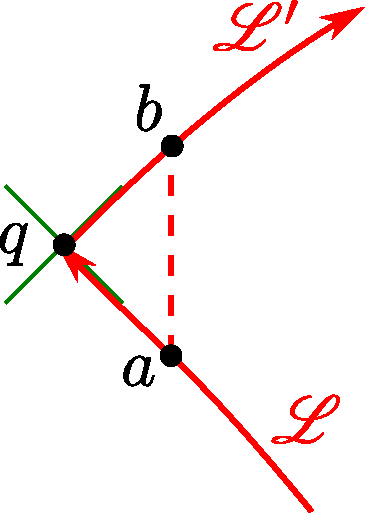
\includegraphics[width=0.17\textwidth]{glo_unique_geod.pdf}}
\caption[]{\label{f:glo:unique_geod} \footnotesize
Proof of Lemma~\ref{p:glo:lem3}.}
\end{figure}
\begin{proof}[Proof of Lemma~\ref{p:glo:lem3}]
Assume that $\Li$ and $\Li'$ have non-collinear tangent vectors at $q$. Then, in
the vicinity of $q$, one can find a point $a\in\Li$ and a point $b\in\Li'$
such that $a$ and $b$ can be connected by a timelike curve (cf.
Fig.~\ref{f:glo:unique_geod}). Since $\Li\subset\Hor$ and $\Li'\subset\Hor$, we have $a\in\Hor$ and
$b\in\Hor$ and therefore we get a contradiction with $\Hor$ being achronal.
\end{proof}
Thanks to Lemma~\ref{p:glo:lem3}, we conclude that $\Li'$ extends $\Li$ to null geodesic
$\Li\cup\Li'$ entirely lying in $\Hor$. By iterating, we conclude that
the null geodesic $\Li$ through $p$ can be extended indefinitely into the
future. Moreover, it can never leave $\Hor$. Indeed, if it leaves $\Hor$ at
some point $q$, by the same procedure used above for $p$, one could construct a future-directed null geodesic
$\Li'\subset\Hor$ starting from $q$ and Lemma~\ref{p:glo:lem3} would imply that
the extension of $\Li$ outside $\Hor$ has to coincide with $\Li'$, which is
in contradiction with $\Li'\subset\Hor$.

Another direct consequence of Lemma~\ref{p:glo:lem3} is that no two distinct null generators
may intersect at a point $p\in\Hor$, except if their segments in the past of
$p$ lie outside $\Hor$.
This completes the proof of Property~\ref{p:glo:prop3}.
\end{proof}


\begin{figure}
\centerline{\includegraphics[width=0.5\textwidth]{glo_BH_headon_gener.jpg}}
\caption[]{\label{f:glo:BH_headon_gener} \footnotesize
Spacetime diagram of the event horizon corresponding to the head-on merger of
two black holes as computed by Matzner et al. (1995) \cite{Matzn_al95}. The
white curves are some null geodesic generators; the left picture is a zoom of
the merger region, with the crease set
(source: Fig.~4 of Ref.~\cite{Matzn_al95}; \copyright 1995 American Association for the Advancement of Science).}
\end{figure}



Some features of Property~\ref{p:glo:prop3} are illustrated in Fig.~\ref{f:glo:BH_headon_gener},
which displays the null geodesic generators in a numerical simulation
of the head-on collision of two black holes by Matzner et al. (1995) \cite{Matzn_al95}.
Note that new null geodesics enter the event horizon at the ``crotch'' of the
``pair of pants''.

The head-on black hole merger has been also computed by Cohen et al. (2009) \cite{CohenPS09}, with an increased numerical accuracy (cf. Fig.~\ref{f:glo:EH_headon_3d}).
Cross-sections of the event horizon $\Hor$ (cf. Sec.~\ref{s:def:spacelike_sections})
are depicted in Fig.~\ref{f:glo:EH_headon}. The same figure shows also how
some null geodesics will reach $\Hor$ to become null generators.


\begin{figure}
\centerline{\includegraphics[width=0.5\textwidth]{glo_EH_headon_3d.jpg}}
\caption[]{\label{f:glo:EH_headon_3d} \footnotesize
Spacetime diagram showing the event horizon in the head-on merger of
two black holes, as computed by Cohen et al. (2009) \cite{CohenPS09}.
The blue curves are null geodesics that will eventually become null generators
of the event horizon; those arising from regions close to the event horizon
are marked by the arrow and the black ellipse
(source: Fig.~15 of Ref.~\cite{CohenPS09}; \copyright 2009 IOP Publishing Ltd).}
\end{figure}

\begin{figure}
\centerline{\includegraphics[width=0.8\textwidth]{glo_EH_headon.jpg}}
\caption[]{\label{f:glo:EH_headon} \footnotesize
Cross-sections (at various coordinate times $t$) of the event horizon $\Hor$ corresponding
to the head-on merger of two black holes as computed by Cohen et al. (2009) \cite{CohenPS09}
and displayed in Fig.~\ref{f:glo:EH_headon_3d}.
Each figure is a 2D cut of a hypersurface $\Sigma_t$ defined by a constant
value of the coordinate time $t$, expressed in units of the sum $M$ of the initial irreducible masses of each black
hole (cf. Sec.~??). The whole 3D hypersurface $\Sigma_t$ can be reconstructed
by rotation around the collision axis.
$t_{\rm CEH}$ (for ``Common Event Horizon'')
is the coordinate time at which the cross-section of $\Hor$ becomes a connected
2-surface.
The cross-sections of $\Hor$ are displayed
in black, while the green dashed curves denote the set of the intersections
with $\Sigma_t$ of the null geodesics that
will become null generators of $\Hor$ through the cusps in the
``individual'' event horizons.
The red and blue dashed curves denotes apparent horizons (cf. Sec.~??).
(source: Fig.~1 of Ref.~\cite{CohenPS09}; \copyright  2009 IOP Publishing Ltd).}
\end{figure}

Finally, Fig.~\ref{f:glo:EH_binspir} shows a cross-section
of the event horizon computed by Cohen et al. (2012) \cite{CohenKS12}
in some inspiralling binary black hole merger. The
black hole spacetime itself has been computed as a solution of the vacuum
Einstein equation (\ref{e:fra:vac_Einstein}) by Scheel at al. \cite{ScheeBCKMP09}; it corresponds to
16 inspiralling orbits of a equal-mass binary black hole with vanishing initial
spins.

\begin{figure}
\centerline{\includegraphics[width=0.6\textwidth]{glo_EH_binspir.jpg}}
\caption[]{\label{f:glo:EH_binspir} \footnotesize
Cross-section of the event horizon $\Hor$ of the inspiralling merger of
two black holes as computed by Cohen et al. (2012) \cite{CohenKS12}.
The $x$ and $y$ axes define the orbital plane.
This cross-section is the first connected one in the slicing of $\Hor$
by surfaces of constant coordinate time $t$
(source: Fig.~2 of Ref.~\cite{CohenKS12}; \copyright 2012 American Physical Society).}
\end{figure}

Generically, for a binary black hole merger,
the crease set forms a 2-dimensional subset of the event horizon
$\Hor$ and is bounded by the set of caustic points, which forms a 1-dimensional
subset of $\Hor$ \cite{Siino98a,Siino98b,HusaW99,CohenKS12}.


\begin{prop}[the event horizon as a null hypersurface]
\label{p:glo:prop4}
Wherever it is smooth, $\Hor$ is a null hypersurface.
\end{prop}

\begin{proof}
Let us assume that $\Hor$ is smooth in some open subset $U$.
By Property~\ref{p:glo:prop2}, $\Hor$ is then a smooth hypersurface in $U$.
According to Property~\ref{p:glo:prop3}, there is a null geodesic lying in $\Hor$ through
any point of $\Hor\cap U$.
This implies null tangent vectors at any point of $\Hor\cap U$, so that, in $U$,
$\Hor$ must be either a null hypersurface or a timelike one. But $\Hor$ is achronal by Property~\ref{p:glo:prop1} and therefore cannot be timelike. Hence, $\Hor$ is a null hypersurface in $U$.
\end{proof}
When $\Hor$ is smooth, its generators,
as defined by Property~\ref{p:glo:prop3}, are then nothing but the
null-hypersurface generators as defined in Sec.~\ref{s:def:geod_gener}.

\begin{remark}
Properties~\ref{p:glo:prop1} to \ref{p:glo:prop4} are not specific to black hole horizons: they are actually
valid for any boundary $\partial J^-(S)$ of the causal past of a given set $S\subset\M$.
They are also valid for the boundary $\partial J^+(S)$ of the causal future of
$S$, modulo the relevant changes future $\leftrightarrow$ past in Property~\ref{p:glo:prop3}.
\end{remark}

It can be shown that event horizons are smooth almost everywhere: the only
location where they are not differentiable is the crease set, i.e. the set of points
where null geodesics cross each other while arriving at $\Hor$ and becoming null
generators.

  % The concept of black hole 3: The global view

\chapter{Stationary black holes}
\label{s:sta}\index{stationary!black hole}

\minitoc

\section{Introduction}

Having defined black holes in all generality in Chap.~\ref{s:glo}, we focus
here on black holes in steady state, i.e. black holes in stationary spacetimes.
We have already discussed
non-expanding horizons and Killing horizons in Chap.~\ref{s:neh} as
possible models for the event horizon of a
steady state black hole. Actually, we shall see here that (each connected
component of) the event horizon of a black hole in a stationary spacetime has to be
a Killing horizon.
We shall start by defining properly the concept of a stationary
spacetime and investigating the first properties of a black hole
in such a spacetime (Sec.~\ref{s:sta:sta_st}). Then, we extend the study of Killing horizons
initiated in Chap.~\ref{s:neh} to encompass bifurcate Killing horizons
(Sec.~\ref{s:sta:bifur_Killing_hor}). In Sec.~\ref{s:sta:mass_angul_mom},
we discuss the concepts
of mass and angular momentum in asymptotically flat spacetimes, which are useful to characterize black holes. In Sec.~\ref{s:sta:EH_KH}, we shall
see that
if the Killing vector $\w{\xi}$ generating stationarity is null on
a connected event horizon $\Hor$, the latter is a Killing horizon with
respect to $\w{\xi}$.  If $\Hor$ is non-degenerate and the
electrovacuum Einstein equation holds, this can only occur in a static spacetime
(\emph{staticity theorem}, Sec.~\ref{s:sta:staticity_thm}).
If on the contrary, $\w{\xi}$ is spacelike on some parts of $\Hor$ (the timelike
case is excluded for the event horizon is a null hypersurface), then, modulo the
electrovacuum Einstein equation and some additional hypotheses,
$\Hor$ is still a Killing horizon, albeit with respect to a Killing vector
distinct from $\w{\xi}$ (\emph{strong rigidity theorem}, Sec.~\ref{s:sta:strong_rigidity}).
Section~\ref{s:sta:Smarr} is devoted to an important relation between various global
quantities characterizing a stationary black hole: the \emph{Smarr formula}.
This is the opportunity to investigate electromagnetic
fields on the horizon of a stationary black hole, in particular to define
the black hole's electric charge and electric potential, both of them being involved
in the Smarr formula. The culmination point of this chapter is
Sec.~\ref{s:sta:no-hair}, which presents the famous
\emph{no-hair theorem}. Modulo some hypotheses, this theorem stipulates that in 4-dimensional
general relativity, all isolated stationary electrovacuum black holes are necessarily
Kerr-Newman black holes; in the pure vacuum case (the most relevant one for astrophysics),
they are Kerr black holes, to be explored in Part.~\ref{P:ker}.

\section{Stationary spacetimes} \label{s:sta:sta_st}

\subsection{Definitions} \label{s:sta:def_station}

\begin{greybox}
A spacetime $(\M,\w{g})$ is called \defin{stationary}\index{stationary!spacetime}
iff (i) it is invariant under
the action of the translation group $(\R,+)$ and (ii) the orbits of
the group action (cf. Sec.~\ref{s:neh:symmetries})
are everywhere timelike curves or (ii') $(\M,\w{g})$
admits a conformal completion (cf. Sec.~\ref{s:glo:conf_compl})
and the orbits of the group action are timelike in the vicinity of
the conformal boundary $\scri$.
It is equivalent to say that there exists a Killing vector field
$\w{\xi}$ (the generator of the translation group, cf. Sec.~\ref{s:neh:symmetries}) that is
timelike everywhere or at least in the vicinity of $\scri$ when there exists a conformal
completion. We shall say that $(\M,\w{g})$ is \defin{strictly stationary}\index{strictly!stationary}\index{stationary!strictly --} iff the Killing vector field $\w{\xi}$ is timelike in all $\M$,
i.e. iff property (ii) above is fulfilled.
\end{greybox}

\begin{remark} \label{r:sta:pseudo-stationary}
Some authors (e.g. Carter \cite{Carte73b}) call
\emph{pseudo-stationary}\index{pseudo-stationary} the stationary spacetimes
that obey (ii'), keeping the qualifier
\emph{stationary} for the strictly stationary case.
As we are going to see, when $\M$
contains a black hole, $\w{\xi}$ cannot be timelike everywhere,
so only \emph{pseudo-stationarity} in Carter's sense is relevant for such spacetimes.
Our terminology, namely keeping the qualifier \emph{stationary} even for (ii'),  follows that of
Choquet-Bruhat \cite{Choqu09},
Chru\'sciel, Lopes Costa \& Heusler \cite{ChrusLH12},
Heusler \cite{Heusl96}
and Wald \cite{Wald01}.
\end{remark}

The Killing vector field $\w{\xi}$ is a priori not unique: the translation group $(\R,+)$
admits the reparametrizations
$t\mapsto t' = \alpha t$, where $\alpha$ is a nonzero constant, which yield
the rescallings $\w{\xi} \mapsto \w{\xi'} = \alpha^{-1} \w{\xi}$
of the Killing vector fields [cf. Eq.~(\ref{e:neh:xi_dxdt})]. When the
spacetime admits a conformal boundary $\scri$ --- which is required if a black hole
is present, given the definition (\ref{e:glo:def_BH}) ---, then
one selects $\w{\xi}$ by demanding that
\be \label{e:sta:xi_scri}
    \w{\xi}\cdot\w{\xi} \to -1 \quad \mbox{near\ } \scri .
\ee
This determines $\w{\xi}$ uniquely, up to a factor $\pm 1$, since this fixes
the rescaling constant $\alpha$ to $\pm 1$. If the spacetime is time-orientable, one
can get rid of the $\pm 1$ ambiguity by demanding that $\w{\xi}$
is future-oriented near $\scri$.

If the stationary spacetime is endowed with electromagnetic and/or
matter fields, they must respect the stationarity as well. For the electromagnetic
field $\w{F}$ (cf. Sec.~\ref{e:fra:electrovacuum}), this is expressed by
the vanishing of the Lie derivative along $\w{\xi}$:
\be
    \Lie{\xi} \w{F} = 0 .
\ee
This condition is similar to Killing-vector property
$\Lie{\xi} \w{g} = 0$ [Eq.~(\ref{e:neh:Lie_xi_g})].

A notion stronger than stationarity is that of \emph{staticity}:

\begin{greybox}
A spacetime $(\M,\w{g})$ is called \defin{static}\index{static!spacetime}
iff (i) it is stationary and (ii) the Killing vector field $\w{\xi}$
generating the stationary action is orthogonal to a family of hypersurfaces
(one says that $\w{\xi}$ is \defin{hypersurface-orthogonal}\index{hypersurface-orthogonal}).
The spacetime $(\M,\w{g})$ is called \defin{strictly static}\index{strictly!static}\index{static!strictly --}
iff moreover $\w{\xi}$ is timelike in all $\M$.
\end{greybox}

\begin{remark}
The same comment as in Remark~\ref{r:sta:pseudo-stationary} can be made: some authors
would call \emph{static} only spacetimes that are
\emph{strictly static} according to the above definition.
\end{remark}

In loose terms, a spacetime is stationary if ``nothing changes with time'', while
it is static if, in addition, ``nothing moves''. A prototype of a stationary
spacetime that is not static is a spacetime containing a steadily rotating
body, be it a star or a black hole.


\subsection{Coordinates adapted to stationarity or staticity}

In a $n$-dimensional stationary spacetime $(\M,\w{g})$, a coordinate system $(x^\alpha) = (x^0, x^1, \ldots  x^{n-1})$
is said \defin{adapted to stationarity}\index{adapted!coordinates} iff the coordinate vector
$\wpar_t$, where $t := x^0$, coincides with the stationary Killing vector $\w{\xi}$.
It has been shown in Sec.~\ref{s:neh:symmetries} that the components $g_{\alpha\beta}$
of the metric tensor with respect to $(x^\alpha)$ then obey $\dert{g_{\alpha\beta}}{t} = 0$
[Eq.~(\ref{e:neh:dgabdt_zero})]. It follows that
\be
   g_{\alpha\beta}  = g_{\alpha\beta}(x^1, \ldots  x^{n-1}) .
\ee
One says that $t$ is an \defin{ignorable coordinate}\index{ignorable coordinate}.

If the spacetime $(\M,\w{g})$ is static, a coordinate system $(x^\alpha) = (x^0=t, x^1, \ldots  x^{n-1})$
is said \defin{adapted to staticity} iff it is adapted to stationarity and the hypersurfaces
$t=\mathrm{const}$ are orthogonal to the static Killing vector $\w{\xi}$.
Given that a normal 1-form to the hypersurfaces $t=\mathrm{const}$ is $\dd t$,
the coordinates $(x^\alpha)$ are adapted to staticity iff
\be \label{e:sta:xi_wpar_t}
    \w{\xi} = \wpar_t \qquad\mbox{and}\qquad \uu{\xi} = W\, \dd t ,
\ee
where $\uu{\xi}$ is the metric dual of $\w{\xi}$ (cf. Sec.~\ref{s:bas:metric_dual})
and $W := \w{g}(\w{\xi},\w{\xi}) = \langle  \uu{\xi}, \w{\xi} \rangle$.
The orthogonality of $\wpar_t$ and the hypersurfaces $t=\mathrm{const}$
translates to $g_{0i}=0$ for $i\in\{1,\ldots,n-1\}$,
the $g_{\alpha\beta}$'s being the metric components with respect to the coordinates
$(x^\alpha)$. Hence one may write the metric of a static spacetime of dimension $n$ as
\be \label{e:sta:static_metric}
    \w{g} = W \dd t^2 + g_{ij} \dd x^i \dd x^j ,
\ee
where the indices $(i,j)$ range in $\{1,\ldots,n-1\}$
and $W$ and $g_{ij}$ are functions of $(x^1,\ldots,x^{n-1})$ only.
It is clear that the metric (\ref{e:sta:static_metric}) is invariant\footnote{Would
(\ref{e:sta:static_metric}) have contained a non-vanishing $g_{0i}\, \D t \, \D x^i$ term,
this would not have been the case.} in the
transformation $t\mapsto-t$. One says that a static spacetime is
\defin{time-reflection symmetric}\index{time!reflection symmetry}\index{reflection!time --}.

\begin{example}[staticity of anti-de Sitter spacetime]
The anti-de Sitter spacetime\index{anti-de Sitter spacetime} AdS$_{4}$ considered in Example~\ref{x:neh:AdS} of Chap.~\ref{s:neh}
is strictly static, with the coordinates $(\tau, r, \th,\ph)$ being
adapted to staticity (hence their name: \emph{global static}).
Indeed, the metric (\ref{e:neh:AdS4}) is of the form (\ref{e:sta:static_metric})
with $t = \tau$ and $W = -\ell^2(1+ r^2)$. The strict staticity follows from $W < 0$, which
shows that the Killing vector $\w{\xi} = \wpar_t$ is everywhere timelike.
\end{example}

\begin{example}[staticity of Schwarzschild spacetime]
The Schwarzschild spacetime\index{Schwarzschild!spacetime}, introduced in Example~\ref{x:def:Schw_hor} of Chap.~\ref{s:def}, is static, but not
strictly static. The staticity is however not obvious from the metric components
given by Eq.~(\ref{e:def:Schw_metric}) because the coordinates
$(t,r,\th,\ph)$ used there are not adapted to staticity: the Killing vector
$\w{\xi} = \wpar_t$ is not orthogonal to the hypersurfaces $t=\mathrm{const}$,
given that $g_{tr} \neq 0$. We shall introduce coordinates adapted to
staticity in Chap.~\ref{s:sch}, namely the \emph{Schwarzschild-Droste coordinates}.
That the Schwarzschild spacetime is not strictly static can be read directly on
Eq.~(\ref{e:def:Schw_metric}): $\w{\xi}\cdot\w{\xi} = g_{tt} = -1 + 2m/r$, so
that $\w{\xi}$ is timelike only in the region $r > 2 m$.
\end{example}

\subsection{Black holes in stationary spacetimes}
\label{s:sta:BH_stationary}

Let us consider a spacetime $(\M,\w{g})$ that \emph{contains a black hole}, as defined in
Sec.~\ref{s:glo:def_BH}. In particular, $(\M,\w{g})$ admits a future
infinity $\scri^+$ and a past infinity $\scri^-$.
Furthermore, we assume that $(\M,\w{g})$ is \emph{stationary},
as defined in Sec.~\ref{s:sta:def_station}.
Since $(\M,\w{g})$ is invariant under the action of the isometry group $(\mathbb{R},+)$,
so is $\scri^+$ (under some proper extension of $\w{\xi}$ to the conformal
completion $\tilde{\M}$)
and therefore its causal past $J^-(\scri^+)$. Since the event horizon $\Hor$
is the boundary of $J^-(\scri^+)$
inside $\M$ [Eq.~(\ref{e:glo:Hor_bound_past_scrip})], we get

\begin{prop}[stationary event horizon]
\label{p:sta:stationary_hor}
The event horizon $\Hor$ of a black hole in a stationary spacetime
is globally invariant under the action of the stationary group $(\R,+)$.
\end{prop}

The word \emph{globally} stresses that
$\Hor$ is invariant \emph{as a whole}, not that
each point of $\Hor$ is a fixed point of the group action.
Let us assume that $\Hor$ is smooth (this sounds likely in a stationary context;
a rigorous proof can be found in Ref.~\cite{ChrusDGH01});
it is then a null hypersurface (Property~\ref{p:glo:prop4} in Sec.~\ref{s:glo:properties_H}).
Now, $\Hor$ is globally invariant if, and only if, the
generator $\w{\xi}$ of the isometry group is tangent to $\Hor$.
Since a timelike vector cannot be tangent to a null hypersurface (cf.
Lemma~\ref{p:def:tangent_to_null_hyp} in Sec.~\ref{s:def:spacelike_sections}), we conclude:

\begin{prop}[stationary Killing vector tangent to the event horizon]
\label{p:sta:xi_tangent_H}
In a stationary spacetime containing a black hole,
the stationary Killing vector field  $\w{\xi}$ is tangent to the event horizon
$\Hor$, which implies that $\w{\xi}$ is either null or spacelike on $\Hor$.
Let $\Hor_0$ be a connected component of $\Hor$
($\Hor_0 = \Hor$ if $\Hor$ is connected).
If $\w{\xi}$ is null on all $\Hor_0$, one says that $\Hor_0$
is \defin{non-rotating}\index{non-rotating horizon}, while if $\w{\xi}$ is
spacelike on some part of $\Hor_0$, one says that $\Hor_0$ is
\defin{rotating}\index{rotating horizon}.
\end{prop}

Since $\w{\xi}$ cannot be timelike on $\Hor$, it follows immediately
that a stationary spacetime containing a black hole cannot be strictly stationary.
We shall discuss in detail the two cases --- null or spacelike --- allowed
for $\w{\xi}$ on $\Hor$ in Sec.~\ref{s:sta:EH_KH}.

It is rather intuitive that the event horizon $\Hor$ of a black hole in
a stationary spacetime must have a vanishing expansion $\theta_{(\wl)}$ along its null
normals $\wl$. Indeed, if $\theta_{(\wl)}$ were nonzero,
the area of cross-sections would vary when dragged
along $\wl$ and this would define some ``evolution'' along $\Hor$ (e.g. from small areas
to larger ones),
which would break the invariance of $\Hor$ under the action of the stationary group.
This of course results from $\Hor$ being part of the global spacetime structure,
since not any null hypersurface in a stationary spacetime has a vanishing
expansion: for instance, a future light cone in Minkowski spacetime
(which is stationary!) has $\theta_{(\wl)}>0$
(cf. Example~\ref{x:def:light_cone6} on p.~\pageref{x:def:light_cone6}),
but the light cone is not invariant by any time translation isometry.
The rigorous proof that $\theta_{(\wl)} = 0$
for stationary event horizons can be found in Hawking \& Ellis' textbook
(Proposition~9.3.1 of Ref.~\cite{HawkiE73}).
Here, we shall simply state:
\begin{prop}[non-expanding horizons for stationary black holes]
\label{p:sta:hor_non_expanding}
The event horizon $\Hor$ of a black hole in a stationary spacetime
is a null hypersurface of vanishing expansion:
\be
    \theta_{(\wl)} = 0 .
\ee
Moreover, if the cross-sections $\Sp$ of $\Hor$
are closed manifolds such that $\Hor$ has the topology $\R\times \Sp$, $\Hor$ is a
\emph{non-expanding horizon}\index{non-expanding!horizon}\index{horizon!non-expanding --},
according to the definition given in Sec.~\ref{s:neh:neh}.
\end{prop}

In dimension 4, one can strongly constrain the topology of the horizon cross-sections:

\begin{prop}[topology theorem 1 \textnormal{(Hawking 1972 \cite{Hawki72})}]
\label{p:sta:topology1}
Let $(\M, \w{g})$ be a 4-dimensional stationary spacetime
containing a black hole of event horizon $\Hor$.
Let $\Sp$ be a connected component of a complete cross-section of $\Hor$.
Let us assume that (i) $\Sp$ is closed (compact without boundary) and orientable;
(ii) the null dominance condition\index{null!dominance condition}\index{dominance!null -- condition} (\ref{e:neh:null_dominant_cond})
is fulfilled on $\Hor$ for some scalar field $f \geq 0$
[for general relativity with $f=\Lambda$
this is equivalent to assuming $\Lambda \geq 0$ and
the dominant null energy condition\index{null!dominant energy condition}\index{energy!condition!null dominant --} (\ref{e:neh:null_dominant_cond_T})]
and (iii) when
displaced into the black hole exterior along $-\w{k}$ (the opposite of
the ingoing null normal $\w{k}$ to $\Sp$),
$\Sp$ becomes a surface with $\theta_{(\wl)} > 0$.
In particular, condition (iii) holds if $\theta_{(\w{k})} < 0$ and there is no trapped
surface (cf. Sec.~\ref{s:neh:trapped_surfaces}) in the black hole exterior.
Then the cross-section $\Sp$
has \emph{generically} the topology of the 2-sphere (i.e. $\Sp$ is
\emph{homeomorphic}\index{homeomorphic} to $\SS^2$). The non-generic case
is that of $\Sp$ having the topology of the 2-torus $\mathbb{T}^2 = \SS^1\times\SS^1$; this can occur only under special circumstances,
among which the metric induced by $\w{g}$ on $\Sp$ must be flat.
\end{prop}

\begin{proof}
Let $\wl$ be a future-directed null normal to $\Hor$ and $\w{k}$ a complementary
future-directed null vector field
normal to $\Sp$, normalized as in Eq.~(\ref{e:def:k_el_minus_one}), i.e.
$\w{k}\cdot\wl = -1$. At each point $p\in \Sp$, the pair $(\w{k},\wl)$ is
a basis of the 2-plane $T_p^\perp\Sp$ orthogonal to $\Sp$ (cf. Fig.~\ref{f:def:TS_ortho}),
with $\wl$ tangent to $\Hor$ and $\w{k}$ transverse to it.
Morever $\w{k}$ points towards the black hole interior, otherwise null geodesics
leaving $\Hor$ along $\w{k}$ would enter $J^-({\scri^+})$.
As in Sec.~\ref{s:def:geom_null_hypsurf}, let us consider that $\Hor$
is the level set $u=0$ of 1-parameter family of hypersurfaces $(\Hor_u)_{u\in\R}$.
This extends $\wl$ in the vicinity of $\Hor$ via Eq.~(\ref{e:def:wl_rho_u})
as a null vector field normal to each $\Hor_u$.
By Property~\ref{p:sta:hor_non_expanding}, we have $\theta_{(\wl)} = 0$
on $\Sp$. Let us displace $\Sp$ by a small parameter $\eps>0$ along $-\w{k}$. The expansion along $\wl$ of the obtained surface is
positive by hypothesis (iii). By taking the limit $\eps\to 0$, we form the
derivative $\Lie{-k} \theta_{(\wl)}$, which must obey
$\Lie{-k} \theta_{(\wl)} \geq 0$ since $\theta_{(\wl)} = 0$ on $\Sp$ and
$\theta_{(\wl)} > 0$ on the displaced surface. Given that
$\Lie{-k} \theta_{(\wl)} = -\Lie{k} \theta_{(\wl)}$, we see that hypothesis
(iii) implies
\be \label{e:sta:Lie_k_l}
    \Lie{k} \theta_{(\wl)} \leq 0 .
\ee
A standard identity (cf. e.g. Eq.~(3b) of \cite{Haywa94}, Eq.~(3.1) of \cite{BoothF07},
Eq.~(5.1) of \cite{Cao11} or Eq.~(36) of \cite{Jaram13})
expresses $\Lie{k}\theta_{(\wl)}$ as
\be \label{e:sta:Lie_k_theta_l}
    \Lie{k} \theta_{(\wl)} = - \frac{1}{2} {}^\Sp\!\! R - \DSc_a \Omega^a
    +  \Omega_a \Omega^a + \w{G}(\wl,\w{k}) ,
\ee
where ${}^\Sp\!\! R$ is the Ricci scalar of the Riemannian metric $\w{q}$ on
$\Sp$ induced by the spacetime metric $\w{g}$, $\DS$ is the Levi-civita
connection associated to $\w{q}$,
$\w{G}$ is the Einstein tensor
of the spacetime metric $\w{g}$ and $\w{\Omega}$ is the 1-form on $\Sp$
that is the pullback of the 1-form $\w{\omega}$ defined by Eq.~(\ref{e:def:def_omega}).
We may also view $\w{\Omega}$ as a spacetime 1-form, defined as
the composition of $\w{\omega}$ with the orthogonal projector $\vw{q}$ onto
$\Sp$: $\w{\Omega} = \w{\omega} \circ \vw{q}$.
In view of Eq.~(\ref{e:def:omega_restrict_H}), we may then write
$\langle\w{\Omega}, \w{v} \rangle = - \w{k} \cdot\wnab_{\vw{q}(\w{v})} \w{\ell}$,
or in index notation, $\Omega_\alpha  = - k_\mu \nabla_\nu \el^\mu q^\nu_{\ \, \alpha}$.
Besides, using Eq.~(\ref{e:neh:null_dominant_cond}), we have
$\w{G}(\wl, \w{k}) = \vw{G}(\wl)\cdot\w{k} = - \w{W}\cdot\w{k} - f \wl\cdot \w{k} = - \w{W}\cdot\w{k} + f$.
Then, integrating (\ref{e:sta:Lie_k_theta_l}) over the compact manifold $\Sp$
and setting the integral of the divergence term $\DSc_a \Omega^a$ to zero since
$\Sp$ has no boundary, we get
\be \label{e:sta:Euler_char}
    \underbrace{\frac{1}{2} \int_\Sp  {}^\Sp\!\! R \, \sqrt{q} \, \D^2 x}_{2\pi\chi} = \int_\Sp \Big[
    \underbrace{\Omega_a \Omega^a}_{\geq 0}
    \, \underbrace{- \w{W}\cdot\w{k}}_{\geq 0}
    + \underbrace{f}_{\geq 0}
    \, \underbrace{- \Lie{k} \theta_{(\wl)}}_{\geq 0} \Big]
          \sqrt{q} \, \D^2 x .
\ee
In the left-hand side, we have invoked the Gauss-Bonnet theorem\index{Gauss-Bonnet theorem}
to express the integral of ${}^\Sp\!\! R$ in terms
of the Euler characteristic\index{Euler characteristic} $\chi$ of the
surface $\Sp$, using the fact that in dimension 2,
the Ricci scalar ${}^\Sp\!\! R$ is twice the
Gaussian curvature\index{Gaussian!curvature}\index{curvature!Gaussian --}.
The signs of the terms of the integrand in the right-hand side
are justified as follows:
$\Omega_a \Omega^a = q^{ab} \Omega_a \Omega_b \geq 0$ because $\w{q}$ is a Riemannian metric,
$- \w{W}\cdot\w{k} \geq 0$ by Lemma~\ref{p:fra:lem2} in Sec.~\ref{s:fra:time_orientation},
given that $\w{k}$ is a future-directed null vector and $\w{W}$ is a future-directed
causal vector thanks to the null dominance condition (\ref{e:neh:null_dominant_cond}),
$f\geq 0$ by hypothesis and $- \Lie{k} \theta_{(\wl)} \geq 0$
follows from Eq.~(\ref{e:sta:Lie_k_l}). Now, the Euler characteristic $\chi$ is a topological
invariant, which is $2$ for the sphere $\SS^2$, $0$ for the torus $\mathbb{T}^2$
and $-2(g-1)$
for a connected orientable surface of genus $g$, i.e. with $g$ ``holes''.
Equation~(\ref{e:sta:Euler_char}) yields $\chi \geq 0$.
The only possibilities for $\Sp$ compact, connected and orientable
are $\SS^2$ ($\chi = 2$) and $\mathbb{T}^2$ ($\chi = 0$).
However the torus case is very special. Indeed, setting $\chi=0$ in Eq.~(\ref{e:sta:Euler_char})
implies that each term in the integrand of the right-hand side vanishes separately:
$\Omega_a \Omega^a = 0$, $\w{W}\cdot\w{k} = 0$, $f=0$ and $\Lie{k} \theta_{(\wl)} = 0$.
The last condition is the marginal case in the inequality (\ref{e:sta:Lie_k_l}). Moreover,
since $\w{q}$ is positive definite, $\Omega_a \Omega^a = 0$ implies $\w{\Omega} = 0$,
which in turn implies $\DSc_a \Omega^a = 0$. In addition,
$\w{G}(\wl, \w{k}) = - \w{W}\cdot\w{k} + f = 0$. We then deduce immediately from
Eq.~(\ref{e:sta:Lie_k_theta_l}) that ${}^\Sp\!\! R = 0$, i.e.
the Ricci scalar of $\w{q}$ is identically zero. Given that the Riemann
curvature tensor of a 2-dimensional metric is proportional to its
Ricci scalar [cf. Eq.~(\ref{e:bas:Riem_n_2})], it follows that $\w{q}$
is a flat metric.
\end{proof}

\begin{remark}
The topology theorem 1, as stated above, is slightly different from the original
version given by Hawking \cite{Hawki72,Hawki73,HawkiE73}, for it adds the ``outermost'' hypothesis (iii). In Hawking's version, (iii) is deduced from the non-existence of
trapped surfaces in the black hole exterior $J^-(\scri^+)$, the latter property
being proved by assumming that the spacetime is globally hyperbolic (Proposition~9.2.8
in Ref.~\cite{HawkiE73}).
Another difference with Hawking's version,
as stated in Proposition~9.3.2 of Ref.~\cite{HawkiE73}, is that
the torus topology is not totally excluded by Property~\ref{p:sta:topology1}.
However, as discussed in
the historical note below, it seems that the exclusion of the torus in
Hawking's proof requires additional hypotheses, which are not explicitely stated
in Refs.~\cite{Hawki72,HawkiE73}.
\end{remark}

\begin{remark}
The topology theorem 1 is not specific to stationary black hole event horizons, for
it relies only on quasilocal properties. Indeed, the proof does not rely on
$\Hor$ being the boundary of a black hole region, if one agrees to define the
``interior'' region as that pointed towards by $\w{k}$. The only required property is
$\Hor$ being a hypersurface (not even a null one)
sliced by spacelike compact surfaces $\Sp$ with
$\theta_{(\wl)} = 0$ and $\Lie{k} \theta_{(\wl)} \leq 0$.
The theorem is therefore valid for \emph{outer trapping horizons} \cite{Haywa94}
and (tubes of) \emph{apparent horizons}, as noticed by Hawking himself \cite{Hawki73} (p.~34),
which are not necessarily null hypersurfaces and which exist in non-stationary spacetimes.
Both concepts of \emph{outer trapping horizon} and \emph{apparent horizon}
will be discussed in Chap.~\ref{s:loc}.
\end{remark}

Another version of the topology theorem relies on the null convergence
condition, which is weaker than the null dominance condition (hypothesis (ii) above),
and replaces hypothesis (iii) by other ones, which are more global. It also
fully excludes the 2-torus topology:

\begin{prop}[topology theorem 2 \textnormal{(Chru\'sciel\index[pers]{Chrusciel, P.T.@Chru\'sciel, P.T.} \& Wald\index[pers]{Wald, R.M.} 1994 \cite{ChrusW94b})}]
\label{p:sta:topology2}
Let $(\M, \w{g})$ be a 4-dimensional asymptotically flat stationary spacetime
containing a black hole of event horizon $\Hor$.
Let us assume that (i) the
null convergence condition\index{null!convergence condition}\index{convergence!condition!null --}  (\ref{e:neh:null_energy_cond}) is fulfilled,
(ii) the domain of outer communications\index{domain of outer communications} $\langle\langle \M\rangle\rangle$
[Eq.~(\ref{e:glo:def_doc})]
is globally hyperbolic,
(iii) $\langle\langle \M\rangle\rangle$ contains an achronal asymptotically
flat hypersurface $\Sigma$ that intersects $\Hor$ in a compact cross-section $\Sp$,
and (iv) some technical condition is fulfilled (cf. \cite{ChrusW94b} for the details).
Then, $\langle\langle \M\rangle\rangle$ is simply connected and
any connected component of $\Sp$ is homeomorphic to the sphere $\SS^2$.
\end{prop}
A part $\mathscr{U}$ of spacetime is said
\defin{globally hyperbolic}\index{globally!hyperbolic}\label{d:sta:glob_hyperbol}
iff it admits a \defin{Cauchy surface}\index{Cauchy!surface}\label{d:sta:Cauchy_surface}, i.e. a spacelike
hypersurface $\Sigma$ such that every inextendible timelike curve of $\mathscr{U}$
intersects $\Sigma$ exactly once (cf. Sec.~8.3 of Wald's textbook~\cite{Wald84} for more
details). We shall not give the proof of Property~\ref{p:sta:topology2} here; it can of course
be found in the original article by Chru\'sciel \& Wald \cite{ChrusW94b}.

\begin{remark}
\label{r:sta:Majumdar_Papapetrou}
The topology theorems 1 and 2 regard only
a \emph{connected component} of a given horizon complete cross-section.
Generally, the latter is a connected 2-manifold, but there exist
4-dimensional stationary (actually static) spacetimes containing a black hole,
the event horizon of which has
disconnected complete cross-sections: the
\emph{Majumdar-Papapetrou spacetimes}\index{Majumdar-Papapetrou!black hole}
\cite{Majum47,Papap47,HartlH72}. They are solutions of the
electrovacuum Einstein equation (cf. Sec.~\ref{e:fra:electrovacuum})
representing an arbitrary number of charged black holes,
which form a static configuration thanks to
an exact balance between the gravitational
attraction and the electrostatic repulsion. The Majumdar-Papapetrou black holes will be discussed
further in Sec.~\ref{s:sta:uniqueness_static} [cf. Eq.~(\ref{e:sta:MajPap_n4})].
\end{remark}

A generalization of the topology theorem 1 to spacetimes of
dimension $n>4$ has been obtained in 2006 by Galloway \& Schoen \cite{GalloS06}
and R\'acz\index[pers]{Racz, I.@R\'acz, I.} provided a simplified
proof of it in 2008 \cite{Racz08}.
However, the theorem for $n>4$ only says that some invariant
of the smooth structure of $\Sp$, called the
\emph{Yamabe invariant}\index{Yamabe invariant}, must be positive for
$f \geq 0$ (\footnote{In brief, Eq.~(\ref{e:sta:Euler_char}) holds for $n>4$
as well, except that the integral of the Ricci scalar ${}^\Sp\!\!R$ is no longer
proportional to the Euler characteristic of $\Sp$ (no Gauss-Bonnet theorem for $\mathrm{dim}\, \Sp \neq 2$ !) but is related to the Yamabe constant of the conformal class of the metric $\w{q}$.}). This result implies that $\Sp$ must admit metrics of positive scalar curvature; it is
less stringent about the topology of $\Sp$ than the theorem for $n=4$.
Actually, the higher $n$, the less constraints on
the topology are provided by the Yamabe invariant. For instance,
for $n=5$, the cross-sections of the \emph{Myers-Perry black holes}\index{Myers-Perry black hole} \cite{MyersP86,EmparR08,Reall14}, which generalize
Kerr black holes to $n>4$, have the
topology of the sphere $\SS^3$, but the topology
$\SS^1\times\SS^2$ is allowed as well, as demonstrated
by the \emph{black ring}\index{black!ring} solution found by Emparan \& Reall \cite{EmparR02,EmparR08,Reall14} (see also Sec.~5.3 of Ref.~\cite{Chrus20}).


\begin{hist}
The topology theorem for the spacetime dimension $n=4$ has been formulated
first by Stephen Hawking\index[pers]{Hawking, S.W.} in 1992 \cite{Hawki72}
(see also p.~34 of Ref.~\cite{Hawki73} and Proposition~9.3.2 in Hawking \& Ellis' textbook
\cite{HawkiE73}).
However, in 1993, Gregory Galloway\index[pers]{Galloway, G.J.} \cite{Gallo94} (p.~119)
pointed out some limitation in Hawking's proof, namely that it cannot
exclude the torus topology ($\chi = 0$) for the horizon's cross-sections
without any extra hypothesis. For instance, for the proof given in Ref.~\cite{Hawki72},
one shall require that the spacetime is \emph{analytic} (cf. Remark~\ref{r:bas:analytic}
in Sec.~\ref{s:bas:def_manif}), which is a rather strong hypothesis.
The proof presented above is based on that given
by Sean Hayward\index[pers]{Hayward, S.} in 1994 \cite{Haywa94}
for outer trapping horizons (see also the proof of Theorem~6.3 in Ref.~\cite{Newma87}).
The theorem obtained by Piotr Chru\'sciel\index[pers]{Chrusciel, P.T.@Chru\'sciel, P.T.}
and Robert Wald\index[pers]{Wald, R.M.} in 1994 \cite{ChrusW94b}
(Property~\ref{p:sta:topology2})
relies on the \emph{topological censorship theorem}\index{topological!censorship theorem} established by
John Friedman\index[pers]{Friedman, J.L.}, Kristin Schleich\index[pers]{Schleich, K.}
and Donald Witt\index[pers]{Witt, D.M.} in 1993 \cite{FriedSW93}.
It leads directly to the spherical topology, excluding the toroidal one.
\end{hist}

%%%%%%%%%%%%%%%%%%%%%%%%%%%%%%%%%%%%%%%%%%%%%%%%%%%%%%%%%%%%%%%%%%%%%%%%%%%%%%%


\section{Bifurcate Killing horizons} \label{s:sta:bifur_Killing_hor}

If the stationary Killing vector $\w{\xi}$,
which is tangent to $\Hor$ by Property~\ref{p:sta:xi_tangent_H},
is null on all $\Hor$, it is then necessarily normal to $\Hor$
(cf. Lemma~\ref{p:def:tangent_to_null_hyp} in Sec.~\ref{s:def:spacelike_sections}).
According to the definition given in Sec.~\ref{s:neh:def_Killing_hor},
$\Hor$ is then a \emph{Killing horizon}.
On the other hand, if $\w{\xi}$ is spacelike on (some parts of) $\Hor$,
we shall see in Sec.~\ref{s:sta:strong_rigidity} that, modulo some
assumptions, the connected components of $\Hor$ are Killing
horizons as well, albeit not with respect to $\w{\xi}$ but to another
Killing vector. This motivates to move on in the study of Killing horizons,
beyond what was achieved in Sec.~\ref{s:neh:Killing_hor}. We shall start
by the concept of bifurcate Killing horizon.

\subsection{Definition and first properties} \label{s:sta:bifur_def}

\begin{greybox}
Let $(\M,\w{g})$ be a $n$-dimensional spacetime endowed with a Killing vector
field $\w{\xi}$. A
\defin{bifurcate Killing horizon}\index{bifurcate!Killing horizon}\index{Killing!horizon!bifurcate --}\index{horizon!bifurcate Killing --} is the
union
\be
    \Hor = \Hor_1 \cup \Hor_2 ,
\ee
such that
\begin{itemize}
\item $\Hor_1$ and $\Hor_2$ are two null hypersurfaces;
\item $\Sp:=\Hor_1\cap\Hor_2$ is a spacelike $(n-2)$-surface;
\item each of the sets $\Hor_1\setminus\Sp$ and $\Hor_2\setminus\Sp$ has two connected components, which are
Killing horizons\footnote{Cf. Sec.~\ref{s:neh:def_Killing_hor} for the
definition of a Killing horizon.} with respect to $\w{\xi}$.
\end{itemize}
The $(n-2)$-dimensional submanifold $\Sp$ is called the
\defin{bifurcation surface}\index{bifurcation!surface} of $\Hor$.
\end{greybox}

\begin{figure}
\centerline{\includegraphics[width=0.5\textwidth]{sta_bifur_Kill_hor.pdf}}
\caption[]{\label{f:sta:bifur_Kill_hor} \footnotesize
Bifurcate Killing horizon $\Hor_1\cup\Hor_2$ with respect to the Killing vector
field $\w{\xi}$; $\Sp$ is the bifurcation surface. $\Li_1$ and $\Li_2$ are
null geodesic generators of respectively $\Hor_1$ and $\Hor_2$, which cross
each other at the point $p\in\Sp$.}
\end{figure}

Hence we may say that a bifurcate Killing horizon is formed by four Killing horizons,
$\Hor_1^+$, $\Hor_1^-$, $\Hor_2^+$ and $\Hor_2^-$ say,
which are merged together at the bifurcation surface $\Sp$ (cf. Fig.~\ref{f:sta:bifur_Kill_hor}), in such a way that
\[
    \Hor_1 = \Hor_1^- \cup \Sp \cup \Hor_1^+ \quad \mbox{and}\quad
    \Hor_2 = \Hor_2^- \cup \Sp \cup \Hor_2^+
\]
are null hypersurfaces.

A first property of bifurcate Killing horizons is
\begin{prop}[vanishing of the Killing vector on the bifurcation surface]
\label{p:sta:xi_S_zero}
The Killing vector field vanishes on the bifurcation surface of
a bifurcate Killing horizon:
\be \label{e:sta:xi_S_zero}
    \encadre{\left. \w{\xi} \right| _{\Sp} = 0 } .
\ee
\end{prop}
\begin{proof}
Let $p\in \Sp$ and let us assume that $\left.\w{\xi}\right| _p\not=0$.
Let $\Li_1$ (resp. $\Li_2$) be the null geodesic generator of $\Hor_1$
(resp. $\Hor_2$) that intersects $\Sp$ at $p$ (cf. Fig.~\ref{f:sta:bifur_Kill_hor}).
By definition of a Killing horizon,
$\w{\xi}$ is tangent to $\Li_1\cap\Hor_1^+$ and to $\Li_1\cap\Hor_1^-$,
i.e. to $\Li_1\setminus\{p\}$.
If $\left.\w{\xi}\right| _p \not=0$, then by continuity,
$\w{\xi}$ is a (non-vanishing) tangent vector field all along $\Li_1$.
Similarly, $\w{\xi}$ is tangent to all $\Li_2$.
At their intersection point $p$, the geodesics $\Li_1$ and $\Li_2$ have thus a common tangent
vector, namely $\left.\w{\xi}\right| _p$.
The geodesic uniqueness theorem (Property~\ref{p:geo:exist_uniq_geod} in Appendix~\ref{s:geo})
then implies $\Li_1 = \Li_2$, so that
$\Li_1 \subset \Hor_1 \cap \Hor_2 = \Sp$. But since $\Sp$ is spacelike and
$\Li_1$ is null, we reach a contradiction. Hence we must have
$\left.\w{\xi}\right| _p = 0$.
\end{proof}

\begin{remark}
\label{r:sta:zero_Killing}
Having a Killing vector field that vanishes somewhere (here $\Sp$) is not the sign
of any pathology: it simply means that the points of $\Sp$ are fixed points of
the isometries generated by $\w{\xi}$, since
setting $\w{\xi}=0$ in Eq.~(\ref{e:neh:xi_dxdt}) leads to $\D\w{x}=0$, i.e.
to $\Phi_{\D t}(p) = p$.
\end{remark}

\begin{remark}
Contrary to what the name may suggest, a bifurcate Killing horizon is \emph{not}
a Killing horizon, for the latter, as defined in Sec.~\ref{s:neh:def_Killing_hor},
is a regular (i.e. embedded) hypersurface
of $\M$ (cf. Sec.~\ref{s:bas:embed} in Appendix~\ref{s:bas}), while
the union of two hypersurfaces is not in general a hypersurface. Moreover
on a Killing horizon, the Killing vector field is nowhere vanishing
[cf. Eq.~(\ref{s:neh:xi_on_KH})], while on
a bifurcate Killing horizon, it is vanishing at the bifurcation surface.
\end{remark}

\begin{example}[bifurcate Killing horizon w.r.t. Lorentz boost]
\label{x:sta:bif-KH-boost}
Let us consider Minkowski spacetime and the boost Killing vector given
by Eq.~(\ref{e:neh:boost-Killing}): $\w{\xi} := x \wpar_t + t \wpar_x$
and let us take for $\Hor_1$ the null hyperplane $t=x$
considered in Example~\ref{x:neh:boostKH} in Chap.~\ref{s:neh} and denoted there
by $\Hor$. The two half-hyperplanes defined by
Eq.~(\ref{e:neh:boost-Killing_hor}) are then the Killing horizons $\Hor_1^+$ and
$\Hor_1^-$. The union $\Hor_1 \cup \Hor_2$, where $\Hor_2$ is the null hyperplane $t=-x$ is a bifurcate Killing horizon with respect to $\w{\xi}$,
with the 2-plane $(t,x)=(0,0)$ as bifurcation surface
(cf. Fig.~\ref{f:sta:hplane_bifur}). Note that on $\Hor_1$, the Killing vector
$\w{\xi}$ points away from $\Sp$, while on $\Hor_2$, it points towards $\Sp$.
\end{example}

\begin{figure}
\centerline{\includegraphics[width=0.6\textwidth]{sta_hplane_bifur.pdf}}
\caption[]{\label{f:sta:hplane_bifur} \footnotesize
Bifurcate Killing horizon $\Hor_1\cup\Hor_2$ with respect to the Killing vector
field $\w{\xi} = x \wpar_t + t \wpar_x$ generating Lorentz boosts in the plane $(t,x)$ of Minkowski spacetime. The dimension along $z$ having been suppressed, the bifurcation
surface $\Sp$ appears as a line, while it is actually a 2-plane.}
\end{figure}



\subsection{Non-degenerate Killing horizons and Boyer's theorem}
\label{s:sta:non-degenerate_KH}

Let us consider a Killing horizon $\Hor$ with respect to some Killing vector
$\w{\xi}$. As shown in Chap.~\ref{s:neh},
modulo some mild condition (the null dominance condition),
the surface gravity\index{surface!gravity} $\kappa$ of $\Hor$
is constant over $\Hor$ (Property~\ref{p:neh:zeroth_law}).
In what follows, we focus on the case where $\kappa\neq 0$, i.e. $\Hor$
is a non-degenerate Killing horizon (cf. Sec.~\ref{s:neh:classif_KH}).
In this case, the parameter $t$ of the null geodesic generators of $\Hor$
associated to $\w{\xi}$ is not affine
(for $\kappa$ is the non-affinity coefficient\index{non-affinity coefficient}
of $\w{\xi}$). However, we may
rescale $\w{\xi}$ to get an affine parameter, at the price of loosing
the Killing vector feature:


\begin{prop}[affine parametrization of a non-degenerate Killing horizon]
Let $\Hor$ be a non-degenerate Killing horizon with respect to
a Killing vector $\w{\xi}$. Let $t$ be the parameter
of the null geodesic generators $\Li$ of $\Hor$
associated to $\w{\xi}$ ($\w{\xi} = \D\w{x}/\D t$ along $\Li$).
The null vector field $\wl$ defined on $\Hor$ by
\be \label{e:sta:el_kappa_xi}
    \wl = \mathrm{e}^{-\kappa t} \, \w{\xi} \quad \iff\quad
    \w{\xi} = \mathrm{e}^{\kappa t} \, \wl ,
\ee
where $\kappa\neq 0$ is $\Hor$'s surface gravity,
is a geodesic vector field and the affine parameter associated to it is
\be \label{e:sta:lambda_t}
    \lambda = \frac{\mathrm{e}^{\kappa t}}{\kappa} + \lambda_0 ,
\ee
where $\lambda_0$ is some constant.
\end{prop}

\begin{proof}
We have
\[
\wnab_{\wl}\, \wl = \wnab_{\mathrm{e}^{-\kappa t} \w{\xi}} \left( \mathrm{e}^{-\kappa t} \, \w{\xi} \right) = \mathrm{e}^{-\kappa t} \wnab_{\w{\xi}} \left( \mathrm{e}^{-\kappa t} \, \w{\xi} \right)
= \mathrm{e}^{-\kappa t} \big[ \big( \underbrace{\wnab_{\w{\xi}} \mathrm{e}^{-\kappa t}}_{\D \mathrm{e}^{-\kappa t}/\D t} \big) \w{\xi}
    + \mathrm{e}^{-\kappa t} \underbrace{\wnab_{\w{\xi}}\, \w{\xi}}_{\kappa\w{\xi}}
    \big] = 0 .
\]
Hence $\wl$ is a geodesic vector. Besides, along any null generator of $\Hor$,
one has [cf. Eq.~(\ref{e:bas:def_vector})]
\[
    \frac{\D\lambda}{\D t} = \w{\xi}(\lambda) = \mathrm{e}^{\kappa t}
    \underbrace{\wl(\lambda)}_{1} = \mathrm{e}^{\kappa t} ,
\]
which, once integrated, yields Eq.~(\ref{e:sta:lambda_t}).
\end{proof}

Let us assume $\kappa>0$ and consider a
null geodesic generator $\Li$ of $\Hor$; $\Li$ can be parameterized by $t$, the corresponding
tangent vector being $\w{\xi}$. When $t$ spans the whole interval $(-\infty,+\infty)$,
Eq.~(\ref{e:sta:lambda_t}) implies that $\lambda$ spans the
interval $(\lambda_0,+\infty)$ only. Since $\lambda$ is an affine parameter of $\Li$,
this means that $\Li$ is an \emph{incomplete} geodesic\index{incomplete geodesic}\index{geodesic!incomplete --} (cf. Sec.~\ref{s:geo:existence_uniqueness}).
Moreover, Eq.~(\ref{e:sta:el_kappa_xi}) leads to
\be \label{e:sta:xi_zero_t_inf}
    \w{\xi} \rightarrow 0 \quad\mbox{when}\quad t\rightarrow -\infty \qquad (\kappa>0).
\ee
In other words, the Killing vector field $\w{\xi}$ vanishes and
the null geodesic $\Li$ stops at the ``edge'' of $\Hor$ corresponding to
$t\rightarrow -\infty$.
If there is no obstacle (spacetime singularity or spacetime edge\footnote{A spacetime edge is generally not a genuine obstacle for extending an incomplete geodesic: it simply indicates
that the spacetime itself needs to be extended so that the geodesic becomes complete,
cf. Remark~\ref{r:sta:extension_bifurcate} below.}),
$\Li$ can be
extended to $\lambda\in(-\infty,\lambda_0]$, giving rise to a complete
null geodesic $\tilde\Li$. This operation can be performed for all the
null geodesic generators of $\Hor$ and we have the freedom to choose the same value
of $\lambda_0$ in Eq.~(\ref{e:sta:lambda_t}) for all of them. In this process,
one gives birth to a null hypersurface, $\tilde\Hor$ say, which contains $\Hor$. Let $\Sp\subset\tilde\Hor$ be the set of points of
affine parameter $\lambda=\lambda_0$ along all the extended null geodesics
$\tilde\Li$. $\Sp$ is clearly a cross-section of $\tilde\Hor$
(cf. Sec.~\ref{s:def:spacelike_sections}); it is then a
spacelike $(n-2)$-dimensional surface.
Assuming that $\w{\xi}$ is future-directed on $\Hor$,
$\Sp$ constitutes the past boundary of $\Hor$, i.e. the boundary corresponding to $t\rightarrow -\infty$.
Since $\w{\xi}$ is a smooth vector field on $\M$, Eq.~(\ref{e:sta:xi_zero_t_inf})
implies that $\w{\xi}$ vanishes on $\Sp$.
In other words, $\Sp$ is a set of fixed points for the isometry group generated
by $\w{\xi}$ (cf. Remark~\ref{r:sta:zero_Killing} above).
Let us denote by $\Hor^-$ the subset of $\tilde\Hor$
generated by the segments $\lambda<\lambda_0$ of the null geodesics $\tilde\Li$:
$\Hor^- = \tilde\Hor\setminus(\Hor\cup\Sp)$.
$\Hor^-$ is clearly a null hypersurface.
Since $\Sp$ is spacelike and $(n-2)$-dimensional, there are, at each point
$p\in\Sp$, only two null directions normal to $\Sp$ (cf. Sec.~\ref{s:def:spacelike_sections}). One of them is along $\wl$. The set of all null geodesics
departing from $\Sp$ along the other null direction forms a null hypersurface,
$\Hor_2^+$ say, in the future of $\Sp$ and another null hypersurface, $\Hor_2^-$
say, in the past of $\Sp$.
By studying the behaviour of a Killing vector field around the set of its
fixed points (here $\Sp$), Boyer \cite{Boyer69} has shown that in
the current setting (i.e. $\Sp$ spacelike), $\w{\xi}$ acts \emph{locally}
as the generator of Lorentz boosts in Minkowski spacetime and $\Sp$ is the bifurcation surface
of a bifurcate Killing horizon similar to that of Example~\ref{x:sta:bif-KH-boost}
(cf. Fig.~\ref{f:sta:hplane_bifur}).
More precisely, Boyer proved the following:

\begin{prop}[Boyer's theorem\index{Boyer's theorem} \textnormal{(Boyer\index[pers]{Boyer, R.H.} 1969 \cite{Boyer69})}]
\label{p:sta:Boyer_thm}
A Killing horizon $\Hor$ is contained in a bifurcate Killing horizon if and
only if $\Hor$ contains at least one incomplete, extendable, null geodesic
generator.
\end{prop}

That $\Hor$ contains an incomplete geodesic is guaranteed by
$\kappa\not=0$, as we have just seen.
It follows that $\Hor^-$, $\Hor_2^+$ and $\Hor_2^-$
are three Killing horizons, so that $\Hor\cup\Hor^-\cup\Hor_2^+\cup\Hor_2^-\cup\Sp$
is a bifurcate Killing horizon.

If $\kappa<0$, we see from Eq.~(\ref{e:sta:lambda_t}) that while $t$ spans the
whole interval $(-\infty,+\infty)$, the affine parameter $\lambda$ spans the
interval $(-\infty,\lambda_0)$ only. Moreover, Eq.~(\ref{e:sta:el_kappa_xi})
leads to
\be
    \w{\xi} \rightarrow 0 \quad\mbox{when}\quad t\rightarrow +\infty  \qquad (\kappa<0).
\ee
The reasoning developed for $\kappa>0$ can be applied mutatis mutandis,
leading to a bifurcate Killing horizon with a bifurcation surface $\Sp$ that
is the future boundary of $\Hor$. Hence we conclude:
\begin{prop}[non-degenerate Killing horizons and bifurcate Killing horizons]
\label{p:sta:non_degen_bifurcate}
The null geodesic generators of a non-degenerate Killing horizon $\Hor$ are
incomplete; if they can be extended, $\Hor$ is contained in a
bifurcate Killing horizon, the bifurcation surface of which is the past
(resp. future) boundary of $\Hor$ if $\kappa>0$ (resp. $\kappa<0$).
\end{prop}

\begin{remark}
\label{r:sta:extension_bifurcate}
It could be that the generators of $\Hor$ cannot be extended simply
because the spacetime $(\M,\w{g})$ is not been chosen ``large enough''.
I.~R\'acz\index[pers]{Racz, I.@R\'acz, I.} and R.M.~Wald\index[pers]{Wald, R.M.} \cite{RaczW96}
have shown that under some mild hypotheses (in particular that $(\M,\w{g})$ is globally
hyperbolic), one can extend $(\M,\w{g})$ to a larger spacetime with a bifurcate
Killing horizon containing $\Hor$.
\end{remark}

\begin{remark}
For a degenerate Killing horizon, the problem of extension disappears, since
$t$ is then an affine parameter of the null generators. Consequently if $t$ spans
the whole interval $(-\infty,\infty)$, the null generators are complete
geodesics. One can still have $\w{\xi}\rightarrow 0$ at some boundary
of $\Hor$, but this is a null boundary, not a spacelike one, and it does not
correspond to a bifurcation surface. An example is the Killing horizon with
respect to a null-rotation Killing vector in Minkowski spacetime, exhibited
as Examples~\ref{x:neh:nullrotKH} and \ref{x:neh:nullrotKH_kappa}
in Chap.~\ref{s:neh}, p.~\pageref{x:neh:nullrotKH} and \pageref{x:neh:nullrotKH_kappa}
respectively (cf. Fig.~\ref{f:neh:hplaneKilling-nullrot}): $\w{\xi}=0$
on the null 2-plane of equation $t=x$, $y=0$.
\end{remark}

\begin{hist} \label{h:sta:Boyer}
The concept of bifurcate Killing horizons has been introduced by Robert H. Boyer\index[pers]{Boyer, R.H.}
(1932-1966), a young American mathematical physicist who had just been appointed
to the University of Liverpool. Sadly, Boyer was killed, among 14 victims, in a mass murder that
occurred in the University of Texas at Austin on 1 August 1966.
His last notes, containing the definition of a bifurcate Killing horizon
and the proof of Property~\ref{p:sta:Boyer_thm}, have been turned into an article
by Jürgen Ehlers\index[pers]{Ehlers, J.} and John Stachel\index[pers]{Stachel, J.L.}, which has
been published in 1969 \cite{Boyer69}.
\end{hist}

%%%%%%%%%%%%%%%%%%%%%%%%%%%%%%%%%%%%%%%%%%%%%%%%%%%%%%%%%%%%%%%%%%%%%%%%%%%%%%%


\section{Mass and angular momentum} \label{s:sta:mass_angul_mom}

For an asymptotically flat stationary spacetime, containing a
black hole or not, there is a well-defined concept of mass: the \emph{Komar mass},
which we introduce here (Secs.~\ref{s:sta:Komar_mass}-\ref{s:sta:Komar_ADM}).
For axisymmetric spacetimes, which are relevant
for stationary rotating black holes, there is in addition the concept
of \emph{Komar angular momentum}, which we shall introduce in Sec.~\ref{s:sta:Komar_angu_mom}.

\subsection{Mass and angular momentum of weakly relativistic stationary systems}
\label{s:sta:weakly_relativistic}

We shall call \defin{weakly relativistic}\index{weakly!relativistic}
a $n$-dimensional spacetime $(\M,\w{g})$
such that $\M$ is diffeomorphic to $\R^n$ and the metric tensor can be expressed as
\be \label{e:sta:weak_g_f_h}
    \w{g} = \w{f} + \w{h} ,
\ee
where $\w{f}$ is a flat Lorentzian metric on $\M$ and $\w{h}$ is small in the following
sense: the components of $\w{h}$ obey $|h_{\alpha\beta}| \ll 1$
in any \defin{Minkowskian coordinates for}\index{Minkowskian coordinates} $\w{f}$, i.e. coordinates
$(x^\alpha)$ on $\M$ such that\footnote{We keep the notation $\eta$ for the matrix $\mathrm{diag}(-1,1,\ldots,1)$, so that
$(\eta_{\alpha\beta})$ stands for the components of $\w{f}$ in Minkowskian coordinates only.}
$(f_{\alpha\beta}) = \eta := \mathrm{diag}(-1,1,\ldots,1)$.
In addition, we assume that $\w{g}$
is ruled by the Einstein equation (\ref{e:fra:Einstein_eq}) with $\Lambda=0$
and an energy momentum tensor $\w{T}$ of compact support.

Given the flat metric $\w{f}$, the Minkowskian coordinates $(x^\alpha)$
are not unique: any Poincaré transformation\index{Poincaré!transformation}\label{p:sta:Poincare_transf}
${\tilde x}^\alpha = \Lambda^\alpha_{\ \, \mu} x^\mu + c^\alpha$, where
$(\Lambda^\alpha_{\ \, \beta})$ is a Lorentz matrix and the $c^\alpha$'s are
constant, leads to a coordinate system $({\tilde x}^\alpha)$ on $\M$ that is Minkowskian for $\w{f}$.
Furthermore, the flat metric $\w{f}$ itself, and hence the decomposition (\ref{e:sta:weak_g_f_h}), is
highly non-unique.
Indeed any change of coordinates of the form ${x'}^\alpha = x^\alpha + \zeta^\alpha(x^0,\ldots,x^{n-1})$
where $(x^\alpha)$ are Minkowskian coordinates for $\w{f}$ and $\zeta^\alpha$ are infinitesimal functions,
leads to the following components of the metric tensor with respect to $({x'}^\alpha)$:
\[
    {g'}_{\alpha\beta} = g_{\mu\nu} \der{x^\mu}{{x'}^\alpha} \der{x^\nu}{{x'}^\beta}
    = \left( \eta_{\mu\nu} + h_{\mu\nu}\right) \left( \delta^\mu_{\ \, \alpha} - \partial_\alpha \zeta^\mu \right)
     \left( \delta^\nu_{\ \, \beta} - \partial_\beta \zeta^\nu \right) ,
\]
where we have used $x^\alpha = {x'}^\alpha - \zeta^\alpha$
and $\dert{\zeta^\alpha}{{x'}^\beta} = \dert{\zeta^\alpha}{x^\sigma} \times \dert{x^\sigma}{{x'}^\beta} \simeq
\dert{\zeta^\alpha}{x^\beta} =: \partial_\beta \zeta^\alpha$ to the first order in $\zeta^\alpha$.
Expanding to the first order in $\zeta^\alpha$ and $\w{h}$, we get
\[
    {g'}_{\alpha\beta}  = \eta_{\alpha\beta} + h_{\alpha\beta}
    - \partial_\alpha \zeta_\beta - \partial_\beta \zeta_\alpha ,
\]
where $\zeta_\alpha := \eta_{\alpha\mu} \zeta^\mu$.
We may recast the above expression as
$\w{g} = \w{f'} + \w{h'}$,
where $\w{f'}$ is the metric whose components in the coordinates $({x'}^\alpha)$ are
$\eta_{\alpha\beta}$ (hence $\w{f'}$ is flat, as\footnote{Note that
the components of $\w{f}$ with respect to the coordinates $({x'}^\alpha)$ are not $\eta_{\alpha\beta}$
but $\eta_{\alpha\beta} - \partial_\alpha \zeta_\beta - \partial_\beta \zeta_\alpha$.} $\w{f}$)
and $\w{h'}$ has the following components with respect to the coordinates $({x'}^\alpha)$:
\be \label{e:sta:hprime_h_zeta}
    {h'}_{\alpha\beta} = h_{\alpha\beta} - \partial_\alpha \zeta_\beta - \partial_\beta \zeta_\alpha .
\ee
The above relation can be viewed as expressing some \emph{gauge freedom}\index{gauge!freedom} on
$\w{h}$. This freedom actually reflects the freedom in the choice of the flat background metric $\w{f}$ in the
decomposition (\ref{e:sta:weak_g_f_h}).

\begin{prop}[Lorenz gauge for the metric perturbation]
The gauge freedom (\ref{e:sta:hprime_h_zeta}) can be used
to ensure that, in terms of $\w{f}$-Minkowskian coordinates $(x^\alpha)$,
the metric perturbation $\w{h}$ fulfills
\be \label{e:sta:Lorenz_h}
    \encadre{ \partial_\mu \left( \eta^{\mu\nu} \bar{h}_{\alpha\nu} \right)  = 0 },
\ee
where
\be \label{e:sta:def_h_bar}
    \w{\bar{h}} := \w{h} - \frac{1}{2} h \, \w{f} ,
\ee
$h$ standing for the trace of $\w{h}$ with respect
to $\w{f}$: $h := \eta^{\mu\nu} h_{\mu\nu}$.
The choice (\ref{e:sta:Lorenz_h}) is referred to as the
\defin{Lorenz gauge}\index{Lorenz gauge} (sometimes
\defin{Hilbert gauge}\index{Hilbert gauge} \cite{Strau13}).
\end{prop}

\begin{proof}
From Eq.~(\ref{e:sta:hprime_h_zeta}), we get $h' := \eta^{\mu\nu} {h'}_{\mu\nu} = h - 2 \partial_\mu \zeta^\mu$,
so that ${\bar{h}}'_{\alpha\beta} = \bar{h}_{\alpha\beta}
- \partial_\alpha \zeta_\beta - \partial_\beta \zeta_\alpha +  \partial_\mu \zeta^\mu \eta_{\alpha\beta}$.
It follows then that $\partial_\mu \left( \eta^{\mu\nu} {\bar{h}'}_{\alpha\nu} \right) =  \partial_\mu \left( \eta^{\mu\nu} \bar{h}_{\alpha\nu} \right) - \Box_{\w{f}} \zeta_\alpha$,
where $\Box_{\w{f}} := \eta^{\mu\nu} \partial_\mu \partial_\nu$ is the d'Alembertian\index{d'Alembertian} operator with respect to $\w{f}$. Accordingly, if the Lorenz gauge (\ref{e:sta:Lorenz_h}) is not fulfilled,
it suffices to solve the d'Alembert equation
\be \label{e:sta:Box_zeta}
    \Box_{\w{f}} \zeta_\alpha = \partial_\mu \left( \eta^{\mu\nu} \bar{h}_{\alpha\nu} \right)
\ee
and plug the solution $\zeta_\alpha$ into Eq.~(\ref{e:sta:hprime_h_zeta})
to get a metric pertubation $\w{h'}$ that obeys the Lorenz gauge.
\end{proof}

\begin{remark}
The Lorenz gauge (\ref{e:sta:Lorenz_h}) is equivalent
to the first-order expansion in $\w{h}$ of
the relation defining \defin{harmonic coordinates}\index{harmonic coordinates}
on $\M$, i.e.
\be
   \Box_{\w{g}} x^\alpha = 0 \iff  \partial_\mu \left( \sqrt{-g} \, g^{\mu\alpha} \right) = 0 .
\ee
\end{remark}

\begin{remark} \label{r:sta:freedom_Lorenz}
The Lorenz gauge does not fully specify the pair $(\w{f},\w{h})$. Indeed, the solutions of the
d'Alembert equation (\ref{e:sta:Box_zeta}) are non-unique: they depend on initial and boundary data.
\end{remark}

A standard computation (see e.g. Chap.~18 of \cite{MisneTW73} or Chap.~5 of \cite{Strau13},
noticing that the computation is independent of the spacetime dimension $n$)
shows that, at first order in $\w{h}$ and in the Lorenz gauge,
the Einstein tensor\index{Einstein!tensor!linearized --} of $\w{g}$ is
\be \label{e:sta:G_box_hb}
    \w{G} = - \frac{1}{2} \Box_{\w{f}} \w{\bar{h}} ,
\ee
where $\Box_{\w{f}}$ stands for the d'Alembertian operator relative to the metric $\w{f}$:
in $\w{f}$-Minkowskian coordinates $(x^\alpha)$,
$\Box_{\w{f}} \bar{h}_{\alpha\beta} = \eta^{\mu\nu} \partial_\mu \partial_\nu \bar{h}_{\alpha\beta}$.

Let us now assume that $(\M,\w{g})$ is a stationary spacetime, with Killing vector
$\w{\xi}$. We may then choose $\w{f}$ so that the $\w{f}$-Minkowskian
coordinates $(x^\alpha)$ are adapted to stationarity, i.e.
$x^0$ is an ignorable coordinate, or equivalently
$\wpar_0=\w{\xi}$. Let then $\Sigma$ be a hypersurface $x^0 = \mathrm{const}$
and $\w{\gamma}$ the metric induced by $\w{f}$ on $\Sigma$.
The coordinates\footnote{Latin indices $i,j,k,\ldots$
range in $\{1,\ldots,n-1\}$, while Greek ones range in $\{0,\ldots,n-1\}$.}
$(x^i)_{1\leq i \leq n-1}$ form
a Cartesian coordinate system of $(\Sigma,\w{\gamma})$:
$\w{\gamma} = \delta_{ij} \, \dd x^i \otimes \dd x^j = (\dd x^1)^2 + \cdots + (\dd x^{n-1})^2$.
The operator $\Box_{\w{f}}$ reduces to the Laplace operator of $\w{\gamma}$,
$\Delta$ say, and, thanks to property (\ref{e:sta:G_box_hb}), the
Einstein equation (\ref{e:fra:Einstein_eq}) becomes a system of
$n(n+1)/2$ independent Poisson equations:
\be \label{e:sta:Delta_h_bar_T}
    \Delta {\bar{h}}_{\alpha\beta} = - 16 \pi T_{\alpha\beta} .
\ee
The solutions are obtained via the Green function of the $(n-1)$-dimensional
Laplace operator:
\be \label{e:sta:hbar_Green_function}
    {\bar{h}}_{\alpha\beta}(x)  = \frac{16\pi}{(n-3)\Omega_{n-2}}
    \int_\Sigma \frac{T_{\alpha\beta}({x'})}{|x - {x'}|^{n-3}} \, \D^{n-1} {x'},
\ee
where $x:=(x^1, \ldots, x^{n-1})$, ${x'} :=({x'}^1, \ldots, {x'}^{n-1})$,
$|x - {x'}|^2 := \sum_{i=1}^{n-1}(x^i - {x'}^i)^2$
and $\Omega_{n-2}$ is the area of the unit sphere $\SS^{n-2}$; the latter is given by the formula
\be \label{e:sta:area_p_sphere}
\Omega_{p} = \frac{2\pi^{(p+1)/2}}{\Gamma((p+1)/2)}, \qquad \mbox{with}\quad
\Gamma(u) := \int_0^{+\infty} t^{u-1} \mathrm{e}^{-t}\,  \D t,
\ee
so that
\be \label{e:sta:area_p_sphere_examples}
   \Omega_2 = 4\pi,\quad \Omega_3 = 2\pi^2,\quad  \Omega_4 = \frac{8}{3} \pi^2, \quad
   \Omega_5 = \pi^3,\ \ldots
\ee

\begin{prop}[asymptotic metric of a weakly relativistic system]
Let $(\M,\w{g})$ be a weakly relativistic stationary spacetime of dimension $n\geq 4$, with
$\w{g}$ obeying the Einstein equation (\ref{e:fra:Einstein_eq}) with $\Lambda=0$
and an energy momentum tensor $\w{T}$ of compact support (the ``source''),
where the energy-density dominates over the spatial stresses (weakly relativistic matter).
Within the Lorenz gauge, there exists
a coordinate system $(x^\alpha)$ such that the metric tensor has the following behavior when
$r:=\sqrt{(x^1)^2 + \cdots + (x^{n-1})^2} \to +\infty$:
\begin{subequations}
\label{e:sta:metric_weakly_relat}
\begin{align}
g_{00} = & - 1 +  \frac{16\pi}{(n-2)\Omega_{n-2}} \frac{M}{r^{n-3}} + \bigO\left( \frac{1}{r^{n-1}} \right)
    \label{e:sta:g00_weakly_relat} \\
g_{0i} = & \frac{8\pi}{\Omega_{n-2}} \frac{J_{ij} x^j}{r^{n-1}} + \bigO\left( \frac{1}{r^{n-1}} \right) \\
g_{ij} = & \left(1 + \frac{16\pi}{(n-2)(n-3)\Omega_{n-2}} \frac{M}{r^{n-3}} \right) \delta_{ij}
+ \bigO\left( \frac{1}{r^{n-2}} \right) ,
\end{align}
\end{subequations}
where
\be \label{e:sta:mass_weakly_relat}
    M := \int_\Sigma T_{00}({x}) \, \D^{n-1} {x}
\ee
and
\be \label{e:sta:J_weakly_relat}
    J_{ij} := \int_\Sigma \left( x^j T_{0i}(x) - x^i T_{0j}(x) \right) \, \D^{n-1} {x} ,
\ee
$\Sigma$ being any hypersurface $x^0 = \mathrm{const}$.
The quantities $M$ and $J_{ij}$ are independent of $\Sigma$ (i.e. of $x^0$)
and are called respectively the \defin{mass} and
the \defin{angular momentum} of the central source.
The coordinates $(x^\alpha)$ correspond to the \emph{central source rest-frame}
and take their origin at the \emph{center of mass}, in the sense
that
\be \label{e:sta:rest_frame_mass_center}
    \int_\Sigma T_{0i}(x)  \, \D^{n-1} {x} = 0
    \qand
    \int_\Sigma {x}^i T_{00}(x) \, \D^{n-1} {x} = 0
\ee
The dominance of the energy-density over
the spatial stresses is expressed in terms of the components of $\w{T}$ with respect to
the coordinates $(x^\alpha)$ as $T_{00} \gg |T_{ij}|$.
\end{prop}

\begin{proof}
Let $(\w{f},\w{h})$ obeys the Lorenz gauge and $(x^\alpha)$ be some corresponding
$\w{f}$-Minkowskian coordinates. By a Poincaré transformation (cf. p.~\pageref{p:sta:Poincare_transf}),
one can inforce (\ref{e:sta:rest_frame_mass_center}).
Far from the source, one may expand
the term $1/|x - {x'}|^{n-3}$ in Eq.~(\ref{e:sta:hbar_Green_function})
in powers of ${x'}^i/r$:
\[
    \frac{1}{|x - {x'}|^{n-3}} = \frac{1}{r^{n-3}} \left( 1 + (n-3) \frac{x^j}{r} \frac{{x'}^j}{r}
        + \bigO\left( \frac{|x'|^2}{r^2} \right) \right) ,
\]
where Einstein's summation convention is assumed on the repeated index
$j\in\{1,\ldots,n-1\}$.
Accordingly, Eq.~(\ref{e:sta:hbar_Green_function}) yields
\be \label{e:sta:bar_h_expand}
    {\bar{h}}_{\alpha\beta}(x)  = \frac{16\pi}{\Omega_{n-2}}
        \left( \frac{1}{(n-3)r^{n-3}} \int_\Sigma T_{\alpha\beta}({x'}) \, \D^{n-1} {x'}
        + \frac{x^j}{r^{n-1}}  \int_\Sigma {x'}^j T_{\alpha\beta}({x'}) \, \D^{n-1} {x'}
         \right)  + \bigO\left( \frac{1}{r^{n-1}} \right) .
\ee
For the component $00$, the first integral in the right-hand side
is nothing but $M$,
as defined by (\ref{e:sta:mass_weakly_relat}), while the second integral
vanishes due to the second equation in~(\ref{e:sta:rest_frame_mass_center}).
Hence, we get
\be \label{e:sta:h_bar_00}
    {\bar{h}}_{00}(x) = \frac{16\pi}{(n-3)\Omega_{n-2}} \frac{M}{r^{n-3}}
     + \bigO\left( \frac{1}{r^{n-1}} \right) .
\ee
Regarding the component $0i$ of Eq.~(\ref{e:sta:bar_h_expand}),
the first integral in the right-hand side vanishes due to the first
equation in~(\ref{e:sta:rest_frame_mass_center}). There remains then
\be \label{e:sta:h_bar_0i}
     {\bar{h}}_{0i}(x) = \frac{16\pi}{\Omega_{n-2}} \frac{x^j}{r^{n-1}}
     \int_\Sigma {x'}^j T_{0i}({x'}) \, \D^{n-1} {x'}
     + \bigO\left( \frac{1}{r^{n-1}} \right)
     =  \frac{8\pi}{\Omega_{n-2}} \frac{J_{ij} x^j}{r^{n-1}} + \bigO\left( \frac{1}{r^{n-1}} \right) ,
\ee
where the second equality follows from the identity
\be \label{e:sta:indent_J}
    J_{ij} = 2  \int_\Sigma {x}^j T_{0i}({x}) \, \D^{n-1} {x} .
\ee
To prove it, consider
\[
    \partial_k (x^i x^j T^{0k}) =  \delta^i_{\ k} x^j T^{0k} + x^i \delta^j_{\  k} T^{0k}
    + x^i x^j \underbrace{\partial_k T^{0k}}_{0}
    = x^j  T^{0i} + x^i  T^{0j} ,
\]
where $\partial_k T^{0k} = 0$ results from the equation of energy-momentum conservation
(\ref{e:fra:divT}) specialized to stationary spacetimes and expressed at 0th order in $\w{h}$.
Integrating over $\Sigma$ and invoking the Gauss-Ostrogradsky theorem to set the integral of
the divergence term $ \partial_k (x^i x^j T^{0k}) $ to zero (since $\w{T}$ is has compact support),
we get
\[
    \int_\Sigma x^j T^{0i}(x) \, \D^{n-1} {x} + \int_\Sigma x^i T^{0j}(x) \, \D^{n-1} {x} = 0 .
\]
In view of the definition (\ref{e:sta:J_weakly_relat}) of $J_{ij}$, the
identity (\ref{e:sta:indent_J}) follows, since $T^{0i} = - T_{0i}$ at the 0th order in $\w{h}$.

Let us now reconstruct $\w{h}$ from $\w{\bar{h}}$. Taking the trace of Eq.~(\ref{e:sta:def_h_bar}) with respect to $\w{f}$
yields $\bar{h} := \eta^{\mu\nu} \bar{h}_{\mu\nu} = h - (h/2) \times n = (2 - n) h / 2$.
Hence we may invert Eq.~(\ref{e:sta:def_h_bar}) to
\be \label{e:sta:h_h_bar}
    \w{h} = \w{\bar{h}} - \frac{\bar{h}}{n-2} \w{f}
    \quad\mbox{with}\quad
    \bar{h} = - \bar{h}_{00} + \bar{h}_{ii} .
\ee
The part\footnote{Note that Einstein's summation convention is used:
$\bar{h}_{ii} = \bar{h}_{11} + \cdots + \bar{h}_{n-1,n-1}$.}
 $\bar{h}_{ii}$ of the trace $\bar{h}$ is deduced from
Eq.~(\ref{e:sta:bar_h_expand}):
\[
    {\bar{h}}_{ii}(x)  = \frac{16\pi}{\Omega_{n-2}}
        \left( \frac{1}{(n-3)r^{n-3}} \int_\Sigma T_{ii}({x'}) \, \D^{n-1} {x'}
        + \frac{x^j}{r^{n-1}}  \int_\Sigma {x'}^j T_{ii}({x'}) \, \D^{n-1} {x'}
         \right)  + \bigO\left( \frac{1}{r^{n-1}} \right) .
\]
The second integral vanishes identically, as it can be seen from the identity
\begin{align}
    \partial_i \left( x^k x^j T^{ik}  - \frac{1}{2} r^2 T^{ij} \right) & =
    \delta^k_{\ i} x^j T^{ik} + x^k \delta^j_{\ i} T^{ik} +
    x^k x^j \underbrace{\partial_i T^{ik}}_{0}
    - r \underbrace{\partial_i r}_{x^i/r} T^{ij} - \frac{1}{2} r^2 \underbrace{\partial_i T^{ij}}_{0} \nonumber \\
    & = x^j T^{ii} = x^j T_{ii} , \nonumber
\end{align}
where $\partial_i T^{ij}=0$ follows from the energy-momentum conservation law (\ref{e:fra:divT}). Hence the integral of $x^j T_{ii}$ over $\Sigma$ is that of the divergence of a vector
field that vanishes outside the source and the Gauss-Ostrogradsky theorem allows one to set it to zero.
We are thus left with
\be \label{e:sta:h_bar_ii}
    {\bar{h}}_{ii}(x)  = \frac{16\pi}{(n-3)\Omega_{n-2}}
        \frac{1}{r^{n-3}} \int_\Sigma T_{ii}({x'}) \, \D^{n-1} {x'}
            + \bigO\left( \frac{1}{r^{n-1}} \right) .
\ee
Gathering Eqs.~(\ref{e:sta:h_bar_00}) and (\ref{e:sta:h_bar_ii}), we get
\[
    \bar{h} = \frac{16\pi}{(n-3)\Omega_{n-2}}
        \frac{1}{r^{n-3}} \left( - M + \int_\Sigma T_{ii}({x'}) \, \D^{n-1} {x'} \right)
            + \bigO\left( \frac{1}{r^{n-1}} \right) .
\]
However, given expression (\ref{e:sta:mass_weakly_relat}) for $M$, the weakly relativistic matter condition
$T_{00} \gg |T_{ij}|$ implies that the integral of $T_{ii}$ over $\Sigma$ is negligible in front of $M$. We conclude that
\[
    \bar{h} = - \bar{h}_{00} + \bigO\left( \frac{1}{r^{n-1}} \right) .
\]
It follows then from Eq.~(\ref{e:sta:h_h_bar}) that, up to terms decaying at least as $1/r^{n-1}$,
\begin{align}
  h_{00} & = \bar{h}_{00} + \frac{\bar{h}_{00}}{n-2} \times (-1) = \frac{n-3}{n-2}\,  \bar{h}_{00} \nonumber \\
  h_{0i} & = \bar{h}_{0i} \nonumber \\
  h_{ij} & = \bar{h}_{ij} + \frac{\bar{h}_{00}}{n-2} \, \delta_{ij} =
    \frac{\bar{h}_{00}}{n-2} \, \delta_{ij} + \bigO\left( \frac{1}{r^{n-2}} \right)
  \nonumber .
\end{align}
The last equality holds because the $1/r^{n-3}$ term in $\bar{h}_{ij}$, which is proportional
to the integral of $T_{ij}$ over $\Sigma$ according to Eq.~(\ref{e:sta:bar_h_expand}),
is negligible in front of the $1/r^{n-3}$ term in $\bar{h}_{00}$, given
that $T_{00} \gg |T_{ij}|$. The above three equations, along with the values
(\ref{e:sta:h_bar_00}) and (\ref{e:sta:h_bar_0i}) for $\bar{h}_{00}$
and $\bar{h}_{0i}$, establish formulas (\ref{e:sta:metric_weakly_relat}) for
the components $g_{\alpha\beta} = \eta_{\alpha\beta} + h_{\alpha\beta}$
of the metric tensor.
\end{proof}

\subsection{Asymptotic expression of the metric in stationary asymptotically flat spacetimes}
\label{s:sta:asymptotic_metric}

Let us now consider a generic (not necessarily weakly relativistic) $n$-dimensional spacetime
$(\M,\w{g})$ that is stationary and asymptotically flat, with $\w{g}$
being ruled by the Einstein equation with $\Lambda=0$ and with $\w{T}$ vanishing in the
asymptotic region.
The decomposition $\w{g} = \w{f} + \w{h}$, with $\w{f}$ flat and $\w{h}$ ``small''
[Eq.~(\ref{e:sta:weak_g_f_h})] still holds in some neighborhood $\mathscr{U}$ of infinity.
Moreover, one can still choose the pair $(\w{f},\w{h})$ such that
the Lorenz gauge (\ref{e:sta:Lorenz_h}) is fulfilled and
the linearized Einstein equation in $\mathscr{U}$ reduces to $\Delta \w{\bar{h}} = 0$
[Eq.~(\ref{e:sta:Delta_h_bar_T}) with $\w{T} = 0$].
There exists then a $\w{f}$-Minkowskian coordinate system $(x^\alpha)$ on $\mathscr{U}$
such that the solution for $\w{g}$ is given
by Eq.~(\ref{e:sta:metric_weakly_relat}) to the lowest order in $1/r$,
the difference being that the constants
$M$ and $J_{ij}$ can no longer be expressed by integrals of the energy-momentum
tensor, as in Eqs.~(\ref{e:sta:mass_weakly_relat}) and (\ref{e:sta:J_weakly_relat}).
This can be shown rigorously by using the expansion in powers of $1/r$ of
the generic solution of $\Delta f = 0$ and the Lorenz
gauge (to set some terms to zero), cf. Exercice~19.3 of MTW \cite{MisneTW73}
or Sec.~5.7 of Straumann's textbook \cite{Strau13} for details.
For a configuration that is not assumed to be weakly relativistic, one
should not limit oneself to the linearized Einstein equation.
However, going beyong the first order expansion in $\w{h}$
does not spoil the first terms in the expansions (\ref{e:sta:metric_weakly_relat}) of
$\w{g}$'s components. This simply adds terms with a higher power
of $1/r$. For instance, for $n=4$, the second order expansion in $\w{h}$ introduces
the term $-2M^2/r^2$ in $g_{00}$ (see the above references for details, as well
as Refs.~\cite{Blanc14,PoissW14} for the nonlinear expansion within a post-Newtonian framework).
We may then assert:


\begin{prop}[asymptotic metric of a stationary asymptotically flat spacetime]
Let $(\M,\w{g})$ be a stationary asymptotically flat spacetime of dimension $n\geq 4$, with
$\w{g}$ obeying the Einstein equation (\ref{e:fra:Einstein_eq}) with $\Lambda=0$
and with the energy-momentum tensor $\w{T}$ vanishing in the
asymptotic region.
There exists a coordinate system $(x^\alpha)$ in the asymptotic region
such that the metric tensor has the following behavior when
$r:=\sqrt{(x^1)^2 + \cdots + (x^{n-1})^2} \to +\infty$:
\begin{subequations}
\label{e:sta:asymptotic_metric}
\begin{align}
g_{00} = & - 1 +  \frac{16\pi}{(n-2)\Omega_{n-2}} \frac{M}{r^{n-3}} + \bigO\left( \frac{1}{r^{n-2}} \right)
   \label{e:sta:asymptotic_g00} \\
g_{0i} = & \frac{8\pi}{\Omega_{n-2}} \frac{J_{ij} x^j}{r^{n-1}} + \bigO\left( \frac{1}{r^{n-1}} \right)
     \label{e:sta:asymptotic_g0i} \\
g_{ij} = & \left(1 + \frac{16\pi}{(n-2)(n-3)\Omega_{n-2}} \frac{M}{r^{n-3}} \right) \delta_{ij}
+ \bigO\left( \frac{1}{r^{n-2}} \right) ,
\end{align}
\end{subequations}
where $\Omega_{n-2}$ is the area of the sphere $\SS^{n-2}$
[Eqs.~(\ref{e:sta:area_p_sphere})-(\ref{e:sta:area_p_sphere_examples})],
$M$ is a constant and $(J_{ij})$ is a constant antisymmetric $(n-1)\times(n-1)$
matrix. Furthermore, by a suitable $\mathrm{SO}(n-1)$ transformation of the coordinates
$(x^i)_{1\leq i\leq n-1}$, $(J_{ij})$ can be brought to the following block diagonal form,
depending only on $p:=[(n-1)/2]$ numbers $J_{(1)}$, $\ldots$, $J_{(p)}$ (possibly
equal to zero):
\be \label{s:sta:J_block_diagonal}
    J_{ij} = \left(\begin{array}{ccccc}
    0 & J_{(1)} &  &  &   \\
    -J_{(1)} & 0 & & & \\
     &  & 0 & J_{(2)} & \\
     &  & -J_{(2)} & 0 & \\
     &  &  & & \ddots
    \end{array}\right) ,
\ee
with the last raw and the last column
containing only zeros if $n$ is even.
\end{prop}
The last assertion follows from the fact that any real antisymmetric matrix $J$
is similar to a matrix $J'$ of the type (\ref{s:sta:J_block_diagonal})
via $J' = P J P^{-1}$, where $P$ is a special orthogonal matrix.

Note that the difference between (\ref{e:sta:asymptotic_metric})
and the asymptotic expansion (\ref{e:sta:metric_weakly_relat}) for
a weakly relativistic system is
$\bigO\left( {1}/{r^{n-2}} \right)$ in Eq.~(\ref{e:sta:asymptotic_g00})
versus $\bigO\left( {1}/{r^{n-1}} \right)$ in Eq.~(\ref{e:sta:g00_weakly_relat}).
As discussed above, this results from nonlinear terms in the expansion of the Einstein equation.


\subsection{Komar mass} \label{s:sta:Komar_mass}

In Newtonian gravity, the mass $M$ of an isolated body is defined
similarly to Eq.~(\ref{e:sta:mass_weakly_relat}), namely by the integral
of the mass density $\rho \sim T_{00}$ over the body. An alternative formula
for $M$ is provided by \defin{Gauss's law}\index{Gauss's law}: $M$ is $-1/(4\pi)$ times the flux of the gravitational field
through any closed surface $\Sp$ surrounding the body, namely
\be \label{e:sta:Newtonian_mass}
    M = \frac{1}{4\pi} \int_{\Sp} \vw{\nabla}{\Phi}\cdot \D \w{S} ,
\ee
where $\Phi$ is the Newtonian gravitational and
$\D \w{S}$ is the area element vector normal to $\Sp$. The above formula
is easily derived when $\Sp$ is a sphere of large radius, using spherical coordinates
$(r,\th,\ph)$. Indeed, for large $r$,
one has $\Phi \sim - M/r$, so that $\vw{\nabla}\Phi \sim (M/r^2) \, \wpar_r$. Given that
$\D \w{S} = r^2 \sin\th \, \D\th\, \D\ph\, \wpar_r$ and $\wpar_r\cdot\wpar_r = 1$,
formula~(\ref{e:sta:Newtonian_mass}) follows. This formula is
actually not restricted to a remote sphere, but is valid for any closed surface
$\Sp$ surrounding the body (this follows from the Gauss-Ostrogradsky theorem and Laplace's equation, $\Delta \Phi = 0$, which holds outside the central body).
Gauss's law (\ref{e:sta:Newtonian_mass}) reflects the ``gravitating aspect'' of the mass, while the
volume integral (\ref{e:sta:mass_weakly_relat}) identifies the mass with the ``amount of matter'' constituting
the central body. The latter definition would yield $M=0$ for any vacuum spacetime
(set $\w{T}=0$ in Eq.~(\ref{e:sta:mass_weakly_relat})) and therefore cannot be used to generalize
the concept of mass to strongly relativistic systems. In  particular, one would certainly
demand $M > 0$ for the gravitating mass of Schwarzschild and Kerr black holes, which are pure vacuum solutions of the Einstein equation.

Accordingly, Gauss's law (\ref{e:sta:Newtonian_mass}), rather than the volume integral
(\ref{e:sta:mass_weakly_relat}), is the good basis for any attempt to
generalize the concept of mass to strongly relativistic spacetimes.
Taking a look at the asymptotic expression (\ref{e:sta:metric_weakly_relat}) of the metric tensor
of a weakly relativistic statrionary system, we notice that
the mass $M$ appears as the coefficient of the dominant $1/r^{n-3}$ term
in the expansion of $g_{00}$, so that one could
recover it by considering the flux integral of $\partial g_{00}/\partial r$ over
a $(n-2)$-dimensional surface at large $r$. In order to have a coordinate-invariant
definition, it is more appropriate to consider the 1-form $\uu{\xi}$ metric-dual
to the stationary Killing vector $\w{\xi}$. Indeed, in any coordinate system
adapted to stationarity, i.e. such that the components of
$\w{\xi}$ are $\xi^\alpha=(1,0,\ldots,0)$, the components of $\uu{\xi}$
are $\xi_\alpha = g_{0\alpha}$, so that in particular $\xi_0 = g_{00}$.
Instead of the partial derivative $\partial g_{00}/\partial r$, a natural coordinate-independent
quantity in then the exterior derivative\index{exterior!derivative}\index{derivative!exterior --} $\dd \uu{\xi}$ (cf. Sec.~\ref{s:bas:ext_deriv}). Since the concept of flux
is naturally conveyed by the integral of the Hodge dual (see e.g. Sec.~16.4.7 of Ref.~\cite{Gourg13}), one arrives at the
definition of mass given below [Eq.~(\ref{e:sta:def_Komar_mass})], named \emph{Komar mass}.
In addition to be coordinate-invariant, it shares the same property as the Newtonian mass (\ref{e:sta:Newtonian_mass}),
namely to be independent from the integration surface outside the central body,
at least within general relativity
(Property~\ref{p:sta:Komar_mass_invariant} below).



\begin{greybox}
Let $(\M, \w{g})$ be an asymptotically flat spacetime of dimension $n \geq 4$
that is stationary,
with stationary Killing vector $\w{\xi}$, normalized such that $\w{\xi}\cdot\w{\xi} \to -1$
near the asymptotic boundary [Eq.~(\ref{e:sta:xi_scri})].
Given a spacelike closed $(n-2)$-surface $\Sp\subset\M$,
the \defin{Komar mass over}\index{Komar!mass}\index{mass!Komar --} $\Sp$ is
defined by
\be  \label{e:sta:def_Komar_mass}
    \encadre{M_{\Sp} := - \frac{n-2}{16\pi(n-3)} \int_{\Sp} \star(\dd \uu{\xi}) },
\ee
where
(i) $\uu{\xi}$ is the 1-form associated to $\w{\xi}$
by metric duality (cf. Sec.~\ref{s:bas:metric_dual}), i.e. the 1-form
of components $\xi_\alpha = g_{\alpha\mu} \xi^\mu$, (ii) $\dd \uu{\xi}$ is
the exterior derivative of $\uu{\xi}$ (cf. Sec.~\ref{s:bas:ext_deriv}, especially Eqs.~(\ref{e:bas:def_ext_1f}) and (\ref{e:bas:def_ext_1f_nab})), namely the 2-form whose components
are
\be \label{e:sta:duxi_nab}
    (\dd \uu{\xi})_{\alpha\beta} =
        \partial_\alpha \xi_\beta - \partial_\beta \xi_\alpha =
        \nabla_\alpha \xi_\beta - \nabla_\beta \xi_\alpha
        = 2 \nabla_\alpha \xi_\beta ,
\ee
the last equality following from the Killing equation (\ref{e:neh:Killing_equation}),
and (iii) $\star(\dd \uu{\xi})$ is the $(n-2)$-form that is the
Hodge dual of the 2-form $\dd \uu{\xi}$. The
\defin{Hodge dual}\index{Hodge dual}\index{dual!Hodge --} of
any $p$-form $\w{A}$ is defined\footnote{See e.g.
Sec.~14.6 of Ref.~\cite{Strau13} or
Sec.~14.5 of Ref.~\cite{Gourg13} for an introduction to Hodge duality.}
as the $(n-p)$-form $\star\w{A}$ given by
\be \label{e:sta:Hodge_dual}
    \star\! A_{\alpha_1\ldots\alpha_{n-p}} := \frac{1}{p!}
        A^{\mu_1\ldots\mu_p} \, \epsilon_{\mu_1\ldots\mu_p\alpha_1\ldots\alpha_{n-p}} ,
\ee
where
$\w{\epsilon}$ is the Levi-Civita tensor associated with the metric $\w{g}$
(cf. Sec.~\ref{s:bas:Levi-Civita_tensor}).
\end{greybox}

We shall check below (Property~\ref{p:sta:Komar_mass_asymp_metric}) that
the Komar mass (\ref{e:sta:def_Komar_mass}) gives the coefficient $M$ that
appears in the asymptotic expansion (\ref{e:sta:asymptotic_metric}) of the
metric tensor.

\begin{remark}
\label{r:sta:Komar_well_posed}
As the integral of a $(n-2)$-form over a $(n-2)$-dimensional manifold, formula
(\ref{e:sta:def_Komar_mass}) is well posed. More precisely, on the $(n-2)$-dimensional
manifold $\Sp$, the theory of integration is defined for $(n-2)$-forms \emph{on} $\Sp$,
while $\star(\dd \uu{\xi})$ is a $(n-2)$-form \emph{on} $\M$. However, any
$(n-2)$-form $\w{\omega}$ on $\M$ yields canonically to a unique $(n-2)$-form
$\iota^* \w{\omega}$ on the
submanifold $\Sp$, by restricting the action of $\w{\omega}$ at each point
$p\in\Sp$ to vectors tangent to $\Sp$. One says that $\iota^* \w{\omega}$ is the
\emph{pullback}\index{pullback} of $\w{\omega}$ to $\Sp$ via the embedding $\iota$ of $\Sp$ in $\M$
(cf. Sec.~\ref{s:bas:Lie}).
\end{remark}

\begin{remark}
The numerical prefactor $- (n-2)/(16\pi(n-3))$ in the definition~(\ref{e:sta:def_Komar_mass})
is adjusted so that for weakly relativistic isolated objects, the Komar mass coincides
with the volume integral of the matter energy density, as it will be shown in
Property~\ref{p:sta:Komar_mass_asymp_metric}.
For $n=4$ (the standard spacetime dimension), this prefactor is $-1/(8\pi)$,
while for $n=5$, it becomes $-3/(32\pi)$.
\end{remark}

\begin{remark}
The Komar mass is not defined for $n \leq 3$. In particular,
formula~(\ref{e:sta:def_Komar_mass}) is ill-posed for $n=3$.
Already in Newtonian gravity, the very concept of gravitational mass is well defined only
for $n \geq 4$. Indeed, in spherical symmetry,
a solution of the Poisson equation\index{Poisson equation} outside the sources ($\Delta \Phi = 0$)
that decays with the radius $r$ exists only for $n \geq 4$: this solution is\footnote{This is easy
to get since in the Euclidean space of dimension $n-1$ the Laplace
operator\index{Laplace operator} is $\Delta\Phi = \frac{1}{r^{n-2}} \derd{}{r} \left( r^{n-2} \derd{\Phi}{r} \right)$
for spherically symmetric fields $\Phi(r)$.}
$\Phi = - K/r^{n-3}$ where the constant $K$ is proportional to the mass $M$ of the central source.
For $n=3$, the solutions of $\Delta \Phi = 0$ are $\Phi = a \ln r + b$ ($a$ and $b$ being constant), while
for $n=2$, they are $\Phi = a r + b$, none of them decaying as $r\to +\infty$.
\end{remark}

In view of Eq.~(\ref{e:sta:Hodge_dual}) with $p=2$ and the last equality in Eq.~(\ref{e:sta:duxi_nab}),
the Komar mass formula (\ref{e:sta:def_Komar_mass}) can be written as
\be \label{e:sta:def_Komar_mass_alt}
    M_{\Sp} = - \frac{n-2}{16\pi(n-3)}  \int_{\Sp}  \nabla^\mu \xi^\nu \,
    \epsilon_{\mu\nu\alpha_1\ldots\alpha_{n-2}} ,
\ee
where $\nabla^\mu \xi^\nu \, \epsilon_{\mu\nu\alpha_1\ldots\alpha_{n-2}}$
stands for the $(n-2)$-form $\w{\omega}$ defined by
\[
  \w{\omega}(\w{u}_1,\ldots,\w{u}_{n-2}) = \nabla^\mu \xi^\nu \,
\epsilon_{\mu\nu\alpha_1\ldots\alpha_{n-2}} u_1^{\alpha_1} \cdots  u_{n-2}^{\alpha_{n-2}}
\]
for any $(n-2)$-tuple of vector fields $(\w{u}_1,\ldots,\w{u}_{n-2})$ tangent to $\Sp$ (cf. Remark~\ref{r:sta:Komar_well_posed} above).

Instead of integrals of $(n-2)$-forms \emph{along} the $(n-2)$-surface $\Sp$, as in (\ref{e:sta:def_Komar_mass})
and (\ref{e:sta:def_Komar_mass_alt}), one may
express the Komar mass as a \emph{flux integral}\index{flux!integral}\index{integral!flux --}, i.e. the integral of a 2-form
contracted with some ``area element'', which is \emph{normal} to $\Sp$.
Let us introduce the latter first.

\begin{prop}[area element bivector normal to a codimension-2 surface]
Given a spacelike $(n-2)$-dimensional surface $\Sp\subset \M$, the
\defin{area element bivector normal to}\index{normal!area element}\index{bivector!area element --}\index{area!element bivector} $\Sp$
is the infinitesimal antisymmetric type-(2,0) tensor field defined on $\Sp$ by
\be
    \D \w{S} := (\w{s} \wedge \w{n}) \, \sqrt{q}\, \D^{n-2} x,
\ee
or, in index notation,
\be \label{e:sta:area_bivector}
     \D S^{\alpha\beta} := (s^\alpha n^\beta - n^\alpha s^\beta) \sqrt{q}\, \D^{n-2} x ,
\ee
where
\begin{itemize}
\item $\w{n}$ is a unit future-directed timelike vector\footnote{Do not confuse the vector $\w{n}$
with the spacetime dimension $n$.} normal to $\Sp$
and $\w{s}$ is a unit spacelike vector normal to $\Sp$
such that (i) $\w{s}$ points towards the ``exterior'' of $\Sp$, i.e.
towards the asymptotically flat end of $(\M, \w{g})$ and
(ii) at each point $p\in\Sp$, $(\w{n},\w{s})$ is an orthonormal basis
of the timelike plane $T^\perp_p\Sp$ normal to $\Sp$ (cf. Fig.~??);
\item $\w{s}\wedge\w{n}$ stands for the \defin{exterior product}\index{exterior!product}
of $\w{s}$ by $\w{n}$: $\w{s}\wedge\w{n} := \w{s}\otimes\w{n} -  \w{n}\otimes\w{s}$
(hence formula (\ref{e:sta:area_bivector}));
\item $\D^{n-2} x := \D x^1 \cdots \D x^{n-2}$, where
$(x^a)=(x^1,\ldots,x^{n-2})$ is a coordinate system on $\Sp$
such that $(\w{n},\w{s},\wpar_1,\ldots,\wpar_{n-2})$ is a right-handed basis of $T_p\M$
for any $p\in\Sp$,
i.e. $\w{\eps}(\w{n},\w{s},\wpar_1,\ldots,\wpar_{n-2}) > 0$;
\item $q := \det(q_{ab})$ is the determinant w.r.t. $(x^a)$ of
the metric $\w{q}$
induced on $\Sp$ by the spacetime metric $\w{g}$.
\end{itemize}
The bivector $\D\w{S}$ is independent of the choice of the coordinates $(x^a)$ on $\Sp$ and of the
orthonormal basis $(\w{n},\w{s})$ of $T^\perp_p\Sp$.
\end{prop}
\begin{proof}
The combination $\sqrt{q}\, \D^{n-2} x = \sqrt{q}\, \D x^1 \cdots \D x^{n-2}$ with
$q := \det(q_{ab})$ is the volume (area)
element of the Riemannian manifold $(\Sp,\w{q})$; it is thus invariant in any change of coordinates
$(x^a) \mapsto ({x'}^a)$. Besides, any two orthonormal bases $(\w{n},\w{s})$
and $(\w{n'},\w{s'})$ of $T_p^\perp\Sp$ having the same orientation
and with $\w{n}$ and $\w{n'}$ both future-directed are necessarily related by a
2-dimensional Lorentz boost (cf. Fig.~??):
\[
   \left\{\begin{array}{l}
    \w{n'} = \cosh\psi \, \w{n} + \sinh\psi \, \w{s} \\
    \w{s'} = \sinh\psi \, \w{n} + \cosh\psi \, \w{s} ,
    \end{array}\right.
\]
where $\psi\in\R$ is the boost rapidity. It follows immediately
that $\w{s'}\wedge\w{n'} = \sinh^2\psi \, \w{n}\wedge\w{s} + \cosh^2\psi \, \w{s}\wedge\w{n}
= ( \cosh^2\psi - \sinh^2\psi )\,  \w{s}\wedge\w{n} = \w{s}\wedge\w{n}$, which
shows that the bivector $\w{s}\wedge\w{n}$, and hence $\D \w{S}$, does not depend on the
choice of the orthonormal basis $(\w{n},\w{s})$.
\end{proof}

The normal area element bivector $\D\w{S}$ appears in the following useful lemma.

\begin{lemma}[flux integral of a 2-form]
\label{p:sta:flux_integ_2form}
For any 2-form $\w{A}$ defined in the vicinity of a spacelike $(n-2)$-dimensional
surface $\Sp$, one has
\be \label{e:sta:int_star_A}
    \int_{\Sp} \star \w{A} = \frac{1}{2} \int_{\Sp} A_{\mu\nu} \, \D S^{\mu\nu} ,
\ee
where the $(n-2)$-form $\star\w{A}$ is the Hodge dual of $\w{A}$, as
defined by Eq.~(\ref{e:sta:Hodge_dual}) with $p=2$.
\end{lemma}
\begin{proof}
Using the definition (\ref{e:sta:Hodge_dual}) with $p=2$, we have
\[
    \int_{\Sp} \star \w{A} =
        \frac{1}{2} \int_{\Sp} A^{\mu\nu} \,
        \epsilon_{\mu\nu\alpha_1\ldots\alpha_{n-2}} =
         \frac{1}{2} \int_{\Sp} \w{A}^\sharp (\w{e}^{(\mu)}, \w{e}^{(\nu)})
                \, \w{\epsilon}(\w{e}_{(\mu)}, \w{e}_{(\nu)}, \D\w{\ell}_{1},
                    \ldots, \D\w{\ell}_{n-2}) ,
\]
where $\w{A}^\sharp$ is the tensor field of components $A^{\alpha\beta}$,
$(\w{e}_{(\alpha)})$ is an orthonormal tetrad such that
$\w{e}_{(0)} = \w{n}$ and $\w{e}_{(1)} = \w{s}$,
$(\w{e}^{(\alpha)})$ is its dual cobasis and $\D\w{\ell}_{1}$, $\ldots$, $\D\w{\ell}_{n-2}$
are displacement vectors forming elementary parallelograms on $\Sp$; for instance
$\D\w{\ell}_{a} = \D x^a \, \wpar_a$ (no summation on $a$)
for $a\in\{1, \ldots, n-2\}$.
Note that the last equality in the above expression results from the very
definition of the integral of a $(n-2)$-form over a $(n-2)$-surface.
Given the definition of the tetrad $(\w{e}_{(\alpha)})$, $(\w{e}_{(2)}, \ldots, \w{e}_{(n-1)})$
is necessarily a basis of the tangent space $T_p\Sp$; consequently
$\D\w{\ell}_{1}$, $\ldots$, $\D\w{\ell}_{n-2}$ are linear combinations of $\w{e}_{(2)}$,
$\ldots$, $\w{e}_{(n-1)}$. Thanks to the alternate character of $\w{\epsilon}$,
we may then restrict the sum over the indices $\mu$ and $\nu$ to
$(\mu,\nu) = (0,1)$ and $(\mu,\nu) = (1,0)$.
Hence
\[
     \int_{\Sp} \star \w{A}
     = \int_{\Sp}
    \w{A}^\sharp (\w{e}^{(0)}, \w{e}^{(1)})
            \, \w{\epsilon}(\w{e}_{(0)}, \w{e}_{(1)}, \D\w{\ell}_{1}, \ldots , \D\w{\ell}_{n-2})
    =  \int_{\Sp} A^{(0)(1)}
    \, \w{\epsilon}(\w{n}, \w{s}, \D\w{\ell}_{1}, \ldots , \D\w{\ell}_{n-2}) .
\]
Now, since $(\w{e}_{(\alpha)})$ is an orthonormal basis,
\[
  A^{(0)(1)} = g^{(0)(\mu)} g^{(1)(\nu)} A_{(\mu)(\nu)} = g^{(0)(0)} g^{(1)(1)}
    A_{(0)(1)} = (-1)\times 1 \times A_{(0)(1)} = - A_{(0)(1)} ,
\]
with
\[
    A_{(0)(1)} = \w{A}(\w{e}_{(0)}, \w{e}_{(1)}) = \w{A}(\w{n}, \w{s})
        = A_{\mu\nu} n^\mu s^\nu = - A_{\mu\nu} s^\mu n^\nu
        = - \frac{1}{2} A_{\mu\nu} (s^\mu n^\nu - n^\mu s^\nu) .
\]
On the other side, we recognize in ${}^\Sp\!\!\w{\epsilon} := \w{\epsilon}(\w{n}, \w{s}, \ldots)$ the
``area'' element $(n-2)$-form on $\Sp$ (see e.g. Sec.~16.4.3 of Ref.~\cite{Gourg13}),
so that we may write, for
$\D\w{\ell}_{a} = \D x^a \, \wpar_a$,
\[
    \w{\epsilon}(\w{n}, \w{s}, \D\w{\ell}_{1}, \ldots , \D\w{\ell}_{n-2}) =
        {}^\Sp\!\!\epsilon_{a_1\ldots a_{n-2}} \, \D\ell_{1}^{a_1}\cdots  \D\ell_{n-2}^{a_{n-2}}
        = \sqrt{q} \, \D x^1 \cdots  \D x^{n-2} .
\]
Gathering the above results and using Eq.~(\ref{e:sta:area_bivector})
establishes Eq.~(\ref{e:sta:int_star_A}).
\end{proof}

Thanks to Lemma~\ref{p:sta:flux_integ_2form}, we may re-express the Komar mass
(\ref{e:sta:def_Komar_mass}) as
\be \label{e:sta:M_Komar_dS}
   M_{\Sp} = - \frac{n-2}{32\pi(n-3)}  \int_{\Sp} (\dd \uu{\xi})_{\mu\nu} \,  \D S^{\mu\nu} .
\ee
Using Eq.~(\ref{e:sta:duxi_nab}), this becomes
\be \label{e:sta:Komar_mass_flux_nabla_xi}
    \encadre{ M_{\Sp} = - \frac{n-2}{16\pi(n-3)} \int_{\Sp} \nabla_\mu \xi_\nu \,  \D S^{\mu\nu} } .
\ee
Alternatively, we may express the exterior derivative in terms of
partial derivatives (first equality in Eq.~(\ref{e:sta:duxi_nab})) and get
\[
    (\dd \uu{\xi})_{\mu\nu} \,  \D S^{\mu\nu} =
    (\partial_\mu \xi_\nu - \partial_\nu \xi_\mu)
    (s^\mu n^\nu - n^\mu s^\nu) \sqrt{q}\, \D^{n-2} x
    = 2 \partial_\mu \xi_\nu  (s^\mu  n^\nu - n^\mu  s^\nu)
    \sqrt{q}\, \D^{n-2} x  .
\]
Equation~(\ref{e:sta:M_Komar_dS}) yields then an expression of $M_{\Sp}$ that
can be used for explicit computations:
\be \label{e:sta:M_Komar_partial_der}
    \encadre{ M_{\Sp} = -\frac{n-2}{16\pi(n-3)}
    \int_{\Sp} \partial_\mu \xi_\nu (s^\mu   n^\nu - n^\mu s^\nu)
    \sqrt{q}\,  \D^{n-2} x } .
\ee

\begin{example}[Komar mass in Schwarzschild spacetime]
\label{x:sta:Komar_mass_Schw}
Let us consider the Schwarzschild spacetime $(\M,\w{g})$
introduced in
Example~\ref{x:def:Schw_hor} of Sec.~\ref{s:def:geom_null_hypsurf}.
In terms of the ingoing Eddington-Finkelstein coordinates $(t,r,\th,\ph)$ used there,
the stationary Killing vector is simply $\w{\xi} = \wpar_t$.
We have $n=4$ and let us choose $\Sp$ to be a 2-sphere defined by $(t,r) = \mathrm{const}$.
The coordinates $(x^a) = (x^1, x^2)$ spanning $\Sp$ are then $(\th,\ph)$.
For the pair of normal vectors to $\Sp$, we choose
$\w{n} = N^{-1} \wpar_t  - 2mN/r \wpar_r$ and $\w{s} = N \wpar_r$, where
$N := (1 + 2m/r)^{-1/2}$. Given the metric (\ref{e:def:Schw_metric}), it is
easy to check that
$\w{g}(\w{n},\w{n}) = -1$, $\w{g}(\w{n},\w{s}) = 0$ and $\w{g}(\w{s},\w{s}) = 1$.
It is also immediate that $\w{g}(\w{n},\wpar_\th) = \w{g}(\w{n},\wpar_\ph) =  0$ and
$\w{g}(\w{s},\wpar_\th) = \w{g}(\w{s},\wpar_\ph) =  0$,
which proves that $\w{n}$ and $\w{s}$ are normal to $\Sp$.
Moreover, $\w{s}$ points towards the exterior of $\Sp$ (since $N>0$) and
$(\w{n},\w{s},\wpar_\th,\wpar_\ph)$ is a right-handed basis. All the hypotheses
stated below Eq.~(\ref{e:sta:area_bivector}) are thus fulfilled and we may use
Eq.~(\ref{e:sta:M_Komar_partial_der}) to evaluate the Komar mass over $\Sp$.
The components $\xi_\alpha$ of $\uu{\xi}$ are easily evaluated via
the components (\ref{e:def:Schw_metric}) of $\w{g}$:
$\xi_\alpha = g_{\alpha\mu} \xi^\nu = g_{\alpha\mu} (\partial_t)^\mu = g_{\alpha t}
= (-1 + 2m/r, 2m/r, 0, 0)$.
The only non-zero derivatives $\partial_\mu\xi_\nu$
are then $\partial_r \xi_t$ and $\partial_r \xi_r$; they are both equal to $-2m/r^2$.
It follows that the integrand in Eq.~(\ref{e:sta:M_Komar_partial_der}) is reduced to only two terms:
\[
  \partial_\mu \xi_\nu (s^\mu   n^\nu - n^\mu s^\nu) =
  \partial_r \xi_t (s^r n^t - n^r s^t) = - \frac{2m}{r^2}
  \left( N \times N^{-1}  + 2m N\times 0 \right) = - \frac{2m}{r^2} .
\]
We read on Eq.~(\ref{e:def:Schw_metric}) that the metric induced on
$\Sp$ is $\w{q} = r^2 \, \dd\th^2 + r^2 \sin^2\, \th \dd\ph^2$, so that $\sqrt{q} = r^2 \sin\th$.
Accordingly, Eq.~(\ref{e:sta:M_Komar_partial_der}) leads to
\[
    M_{\Sp} = -\frac{1}{8\pi} \int_{\Sp} \left( - \frac{2m}{r^2} \right)
    r^2 \sin\th \, \D\th \, \D\ph = \frac{m}{4\pi} \int_{\Sp} \D\th \, \D\ph .
\]
Since the remaining integral is nothing but $4\pi$, we get simply
\be \label{e:sta:Komar_mass_Schwarz}
    M_{\Sp} = m.
\ee
We note that $M_{\Sp}$ does not depend on $r$, i.e. does not depend on the
choice of the sphere $\Sp$.
\end{example}

More generally, we have:

\begin{prop}[Komar mass in the asymptotic expression of the metric]
\label{p:sta:Komar_mass_asymp_metric}
The coefficient $M$ that appears in expression (\ref{e:sta:asymptotic_metric})
of the metric tensor of a stationary asymptotically flat $n$-dimensional spacetime
in some asymptotically Minkowskian coordinates $(x^\alpha)$
coincides in the limit $r := \sqrt{(x^1)^2 + \cdots + (x^{n-1})^2} \to +\infty$ with
the Komar mass over the sphere $\Sp$
of constant $(x^0,r)$.
In particular, for a weakly relativistic system, the Komar mass over $\Sp$ is equal
to the volume integral of the matter energy density $T_{00}$, as given by formula
(\ref{e:sta:mass_weakly_relat}).
\end{prop}

\begin{proof}
Without any loss of generality, the coordinate system $(x^\alpha)$ leading
to the expansion (\ref{e:sta:asymptotic_metric}) can be chosen to be adapted
to stationarity, i.e. such that  $\wpar_0 = \w{\xi}$, where $\w{\xi}$ is the
stationary Killing vector.
Let us evaluate the Komar mass $M_\Sp$
via the integral (\ref{e:sta:M_Komar_partial_der}),
denoting the surface element of $\Sp$ by $\sqrt{q} \, \D^{n-2} y$
instead of $\sqrt{q} \, \D^{n-2} x$  to avoid any
confusion with the asymptotically Minkowskian coordinates $(x^\alpha)$.
We have $\xi_\alpha = g_{\alpha\mu} \xi^\mu = g_{\alpha\mu} \delta^\mu_{\ \, 0} =  g_{\alpha 0}$,
with $g_{\alpha 0} = g_{0\alpha}$ given by formulas (\ref{e:sta:asymptotic_metric}) for large $r$,
so that
\[
    \partial_0 \xi_\alpha = 0, \quad
    \partial_i \xi_0 \simeq - \frac{n-3}{n-2} \frac{16\pi}{\Omega_{n-2}} \frac{M}{r^{n-2}} \frac{x^i}{r}
    \quad \mbox{and} \quad
    \partial_i \xi_j \simeq \frac{8\pi}{\Omega_{n-2}} \frac{J_{jk}}{r^{n-1}}
    \left( \delta_{ki} - (n-1) \frac{x^k x^i}{r^2} \right) .
\]
On the other hand, for $r\to +\infty$, we have
$s^\alpha \simeq \left(0,\frac{x^1}{r}, \ldots,\frac{x^{n-1}}{r} \right)$,
$n^\alpha \simeq (1, 0, \ldots, 0)$ and $\sqrt{q} \, \D^{n-2}y = r^{n-2} \sqrt{\bar{q}} \, \D^{n-2} y$,
where $\bar{q}$ stands for the determinant of the round metric of the unit sphere $\SS^{n-2}$ with
respect to the coordinates $(y^1,\ldots,y^{n-2})$. Given that $\partial_i \xi_j$ decays as $1/r^{n-1}$,
it follows that only the terms
involving $\partial_i \xi_0$ contribute to the integral (\ref{e:sta:M_Komar_partial_der}), which becomes
\begin{align}
    M_{\Sp} & = -\frac{n-2}{16\pi(n-3)}
    \int_{\Sp} \partial_i \xi_0 \left( \frac{x^i}{r} \times 1 - 0\times 0 \right) r^{n-2} \sqrt{\bar{q}} \, \D^{n-2} y
    = \frac{M}{\Omega_{n-2}} \int_{\Sp} \underbrace{\frac{x^i}{r} \frac{x^i}{r}}_{1}
     \sqrt{\bar{q}} \, \D^{n-2} y \nonumber \\
     & = \frac{M}{\Omega_{n-2}} \underbrace{ \int_{\Sp} \sqrt{\bar{q}} \, \D^{n-2} y }_{\Omega_{n-2}} .
       \nonumber
\end{align}
Hence $M_{\Sp} = M$. The statement about a weakly relativistic system is an immediate consequence
of expansion (\ref{e:sta:metric_weakly_relat}) being a particular case of
(\ref{e:sta:asymptotic_metric}), given that $M$ in (\ref{e:sta:metric_weakly_relat}) has
the integral form (\ref{e:sta:mass_weakly_relat}).
\end{proof}


\subsubsection{Volume integral formula for the Komar mass}

We are going to derive a volume integral formula for $M_{\Sp}$, from which one can show
the independence of $M_{\Sp}$ from the choice of $\Sp$ in
the vacuum case, thereby generalizing the result of Example~\ref{x:sta:Komar_mass_Schw}.
To this aim, we shall make use of the following lemma:

\begin{lemma}[flux integral of the divergence of a 2-form]
\label{p:sta:flux_div_2_form}
In a $n$-dimensional asymptotically flat spacetime $(\M, \w{g})$,
let $\Sigma$ be a compact spacelike hypersurface bounded by two closed $(n-2)$-surfaces:
an ``internal'' one, $\Sp_{\rm int}$, and an ``external'' one,
$\Sp_{\rm ext}$, the exterior direction being that of the asymptotic flat end of $(\M, \w{g})$.
Let $\w{n}$ be the future-directed unit normal to $\Sigma$ and $\D\w{V}$
the \defin{normal volume element vector}\index{normal!volume!element}\index{volume!normal -- element}
of $\Sigma$ defined by [compare Eq.~(\ref{e:sta:area_bivector})]:
\be \label{e:sta:normal_vol_element}
    \D V^\alpha := - n^\alpha \sqrt{\gamma} \, \D x^1 \cdots \D x^{n-1}
    =: - n^\alpha \sqrt{\gamma} \, \D^{n-1} x,
\ee
where $(x^1, \ldots, x^{n-1})$ stands for a coordinate system on $\Sigma$ and
$\gamma := \det (\gamma_{ij})$  is the determinant w.r.t. these coordinates of the metric
$\w{\gamma}$ induced on $\Sigma$ by the spacetime metric $\w{g}$, so that
$\sqrt{\gamma}\, \D x^1 \cdots \D x^{n-1}$ is the volume element on $\Sigma$.
Then, for any 2-form $\w{A}$, we have
\be \label{e:sta:flux_div_2form}
    2 \int_{\Sigma} \nabla^\nu A_{\mu\nu} \, \D V^\mu
    = \int_{\Sp_{\rm ext}} A_{\mu\nu} \, \D S^{\mu\nu}
      - \int_{\Sp_{\rm int}} A_{\mu\nu} \, \D S^{\mu\nu} ,
\ee
where $\D S^{\mu\nu}$
is defined by Eq.~(\ref{e:sta:area_bivector}) with $\w{s}$ pointing to the
asymptotic flat end of $(\M,\w{g})$ for both $\Sp_{\rm ext}$ and $\Sp_{\rm int}$.
\end{lemma}
\begin{proof}
Let $(t,x^1, \ldots, x^{n-1})$ be a local coordinate system adapted to $\Sigma$,
i.e. such that $\Sigma$ is the hypersurface $t=0$, and let $\w{V}$
be the vector defined by $\uu{V} := \w{A}(., \w{n})$, i.e.
$V_\alpha := A_{\alpha\mu} n^\mu$. Thanks to the antisymmetry of $\w{A}$,
$\w{V}$ is tangent to $\Sigma$: $\w{n}\cdot\w{V} = \w{A}(\w{n},\w{n}) = 0$.
We have then, using the antisymmetry of $\w{A}$,
\bea
    \nabla^\nu A_{\mu\nu} \, \D V^\mu &= & \nabla^\nu A_{\nu\mu} \, n^\mu \sqrt{\gamma} \,  \D^{n-1} x
    = \left( \nabla^\nu V_\nu - A_{\nu\mu} \nabla^\nu n^\mu \right) \sqrt{\gamma} \,  \D^{n-1} x
        \nonumber \\
   & = &
   ( \nabla_\mu V^\mu  + \underbrace{A_{\nu\mu} K^{\nu\mu}}_{0}
    + \underbrace{A_{\nu\mu} n^\nu}_{-V_\mu} D^\mu \ln N ) \sqrt{\gamma} \,  \D^{n-1} x
    \nonumber \\
  & = & \left( \nabla_\mu V^\mu - V^i \partial_i \ln N \right) \sqrt{\gamma} \,  \D^{n-1} x . \nonumber
\eea
In the second line, we have expressed the derivative of $\w{n}$ in terms of the
extrinsic curvature\index{extrinsic curvature}\index{curvature!extrinsic --}
tensor $\w{K}$ of $\Sigma$ and of the lapse function $N := - \w{n} \cdot \wpar_t$,
via the identity $\nabla^\alpha n^\beta = - K^{\alpha\beta} - D^\beta\ln N n^\alpha$
(see e.g. Eq.~(4.24) of Ref.~\cite{Gourg12}), where $D^\beta \ln N = \nabla^\beta \ln N + n^\beta n^\mu \nabla_\mu \ln N$. To get the third line, we have used the symmetry of $\w{K}$
to set $A_{\nu\mu} K^{\nu\mu} = 0$ and the property $V_\mu n^\mu = 0$
to write $V_\mu D^\mu \ln N = V_\mu \nabla^\mu \ln N = V^\mu \partial_\mu \ln N
= V^i\partial_i \ln N$ ($i\in\{1,\ldots,n-1\}$).
Let us now use formula (\ref{e:bas:div_vect}) for the divergence of $\w{V}$,
along with $V^0 = 0$ ($\w{V}$ is tangent to $\Sigma$) and
the relation $\sqrt{-g} = N\sqrt{\gamma}$ between the determinants
of the metrics $\w{g}$ and $\w{\gamma}$ (see e.g. Eq.~(5.55) of Ref.~\cite{Gourg12})
\bea
    \nabla_\mu V^\mu  & = & \frac{1}{\sqrt{-g}} \partial_\mu \left( \sqrt{-g} V^\mu \right)
    = \frac{1}{N \sqrt{\gamma}} \partial_i \left( N \sqrt{\gamma} V^i \right) \nonumber \\
    & = & \frac{1}{\sqrt{\gamma}} \partial_i \left( \sqrt{\gamma} V^i \right)
      + V^i \partial_i \ln N
    = D_i V^i + V^i \partial_i \ln N  ,  \nonumber
\eea
where $D_i V^i$ is the divergence of $\w{V}$ considered as a vector field
on $(\Sigma, \w{\gamma})$, $\w{D}$ standing for the Levi-Civita connection
of $\w{\gamma}$. Hence we get
\[
   \nabla^\nu A_{\mu\nu} \, \D V^\mu = D_i V^i  \sqrt{\gamma}  \, \D^{n-1} x.
\]
We may then apply the Gauss-Ostrogradsky theorem to $\w{V}$
and write the integral of the divergence of $\w{A}$ as
\bea
    \int_{\Sigma} \nabla^\nu A_{\mu\nu} \, \D V^\mu & = &
    \int_{\Sigma}  D_i V^i  \sqrt{\gamma}  \, \D^{n-1} x =
    \int_{\partial\Sigma} \sigma^i V_i \sqrt{q} \, d^{n-2} x \nonumber \\
    & =  &  \int_{\Sp_{\rm ext}}\!\! s^i V_i \sqrt{q} \, d^{n-2} x
        - \int_{\Sp_{\rm int}} \!\! s^i V_i \sqrt{q} \, d^{n-2} x , \nonumber
\eea
where $\w{\sigma}$ is the unit vector normal to the boundary $\partial\Sigma$
and outward-pointing with respect to $\Sigma$. In the present case, $\partial\Sigma$
has two connected components: $\Sp_{\rm int}$ and $\Sp_{\rm ext}$, with
$\w{\sigma} = - \w{s}$ on $\Sp_{\rm int}$ and $\w{\sigma} = \w{s}$ on $\Sp_{\rm ext}$,
hence the last equality.
Now, using again the antisymmetry of $\w{A}$,
\[
   s^i V_i = s^\mu V_\mu = s^\mu A_{\mu\nu} n^\nu = \frac{1}{2} A_{\mu\nu}
   (s^\mu n^\nu - n^\mu s^\nu) .
\]
In view of expression (\ref{e:sta:area_bivector}) for $\D S^{\mu\nu}$, we
thus get $2 s^i V_i \sqrt{q} \, \D^{n-2} x = A_{\mu\nu} \D S^{\mu\nu}$, so
that Eq.~(\ref{e:sta:flux_div_2form}) follows.
\end{proof}

Let us apply Lemma~\ref{p:sta:flux_div_2_form} to the 2-form $\w{A} := \dd \uu{\xi}$, i.e.
to the 2-form of components
$A_{\alpha\beta} := \nabla_\alpha \xi_\beta - \nabla_\beta \xi_\alpha = 2 \nabla_\alpha \xi_\beta $
[cf. Eq.~(\ref{e:sta:duxi_nab})]. The 1-form $2 \nabla^\nu A_{\mu\nu}$ which appears in
the left-hand side of Eq.~(\ref{e:sta:flux_div_2form}) is then, up to a sign,
the metric dual of a vector field $\w{J}$ called the
\defin{Komar current of}\index{Komar!current}\index{current!Komar --}
$\w{\xi}$:  $2 \nabla^\nu A_{\mu\nu} = - J_\mu$, where
\be \label{e:sta:def_Komar_current}
    J^\alpha := - 2 \nabla_\mu \left( \nabla^\alpha \xi^\mu - \nabla^\mu \xi^\alpha \right) .
\ee
The Komar current is actually a conserved current, independently of the Killing nature of $\w{\xi}$:

\begin{prop}[Conservation of the Komar current]
For any vector field $\w{\xi}$ defined on the spacetime $(\M,\w{g})$ (not necessarily a Killing vector field), the Komar current defined by Eq.~(\ref{e:sta:def_Komar_current}) is conserved:
\be \label{e:sta:divJ_zero}
    \nabla_\mu J^\mu = 0 .
\ee
\end{prop}
\begin{proof}
We have, from the definition (\ref{e:sta:def_Komar_current}),
$J^\alpha = - 2 \nabla_\nu A^{\alpha\nu}$ with
$A^{\alpha\beta} :=  \nabla^\alpha \xi^\beta - \nabla^\beta \xi^\alpha$.
Let $(x^\alpha)$ be a coordinate system on $\M$.
Since $\w{A}$ is antisymmetric, its divergence can be expressed in terms of partial derivatives as
$\nabla_\nu A^{\alpha\nu} = \partial_\nu \left( \sqrt{-g} A^{\alpha\nu} \right) / \sqrt{-g}$,
where $g$ is the determinant of $\w{g}$ with respect to $(x^\alpha)$.
Similarly the divergence of $\w{J}$ can be written as
$\nabla_\mu J^\mu  =  \partial_\mu \left( \sqrt{-g} J^\mu \right) / \sqrt{-g}$.
Combining the above formulas leads to
$\nabla_\mu J^\mu = -2 \partial_\mu \partial_\nu  \left( \sqrt{-g} A^{\mu\nu} \right) /  \sqrt{-g}$.
Since $\partial_\mu \partial_\nu = \partial_\nu \partial_\mu$ and $A^{\mu\nu} = - A^{\nu\mu}$,
we get immediately $\nabla_\mu J^\mu = 0$.
\end{proof}

Thanks to the identities $A_{\alpha\beta} = 2 \nabla_\alpha \xi_\beta$ and
$J_\alpha = - 2 \nabla^\mu A_{\alpha\mu}$, we may use Lemma~\ref{p:sta:flux_div_2_form} to write
\[
   -  \int_{\Sigma} J_\mu \, \D V^\mu
    = 2 \int_{\Sp_{\rm ext}} \nabla_\mu \xi_\nu \, \D S^{\mu\nu}
      - 2 \int_{\Sp_{\rm int}} \nabla_\mu \xi_\nu \, \D S^{\mu\nu} .
\]
Using expression~(\ref{e:sta:Komar_mass_flux_nabla_xi}) of the Komar mass,
we get
\be \label{e:sta:Komar_mass_vol_integ_J}
    \encadre{ M_{\Sp_{\rm ext}} = M_{\Sp_{\rm int}} + \frac{n-2}{32\pi(n-3)}
    \int_{\Sigma} J_\mu \, \D V^\mu } .
\ee

Thanks to the Killing equation (\ref{e:neh:Killing_equation}),
expression (\ref{e:sta:def_Komar_current}) for the Komar current $\w{J}$
simplifies to  $J^\alpha = - 4 \nabla_\mu \nabla^\alpha \xi^\mu$.
Now, the Ricci identity (\ref{e:bas:Ricci_ident})
applied to the vector field $\w{\xi}$ yields
$\nabla_\alpha \nabla_\beta \xi^\gamma - \nabla_\beta \nabla_\alpha \xi^\gamma
= R^\gamma_{\ \  \nu \alpha\beta} \, \xi^\nu$. Contracting on the indices
$\alpha$ and $\gamma$ makes the Ricci tensor $R_{\alpha\beta}$ appear:
$\nabla_\mu \nabla_\beta \xi^\mu - \nabla_\beta \nabla_\mu \xi^\mu = R_{\mu\beta} \xi^\mu$.
Thanks to the Killing equation (\ref{e:neh:Killing_equation}), the divergence
of $\w{\xi}$ is zero: $\nabla_\mu \xi^\mu = 0$. Using the symmetry of the Ricci tensor,
we then get the following identity, valid for any Killing vector:
\be
    \encadre{ \nabla_\mu \nabla_\alpha \xi^\mu = R_{\alpha\mu} \xi^\mu } .
\ee
Accordingly, the Komar current of $\w{\xi}$ can be written as
\be \label{e:sta:J_Killing_Ricci}
    \encadre{ J^\alpha = - 4 R^\alpha_{\ \, \mu} \xi^\mu } .
\ee
Pluging this relation into formula (\ref{e:sta:Komar_mass_vol_integ_J})
and using expression~(\ref{e:sta:normal_vol_element}) for $\D V^\mu$,
we arrive at the following property.

\begin{prop}[volume integral formula for the Komar mass]
\label{p:sta:Komar_mass_vol_integ}
Let $(\M, \w{g})$ be an asymptotically flat stationary $n$-dimensional spacetime,
with stationary Killing vector $\w{\xi}$.
Let $\Sigma$ be a compact spacelike hypersurface bounded by two closed $(n-2)$-surfaces:
an ``internal'' one, $\Sp_{\rm int}$, and an ``external'' one,
$\Sp_{\rm ext}$, the exterior direction being that of the asymptotic flat end of $(\M, \w{g})$.
The Komar masses over $\Sp_{\rm ext}$ and $\Sp_{\rm int}$ are then
related by
\be \label{e:sta:Komar_mass_vol_integ_R}
    \encadre{ M_{\Sp_{\rm ext}} = M_{\Sp_{\rm int}} + \frac{n-2}{8\pi(n-3)}
    \int_{\Sigma} \w{R}(\w{\xi}, \w{n}) \sqrt{\gamma} \, \D^{n-1} x , }
\ee
where $\w{R}$ is the Ricci tensor of $\w{g}$,
$\w{n}$ is the future-directed unit normal to $\Sigma$
and $\sqrt{\gamma}\,\D^{n-1} x$ is the volume element on $\Sigma$
induced by $\w{g}$.
If $\w{g}$ obeys the Einstein equation (\ref{e:fra:Einstein_eq_n}) with some energy-momentum
tensor $\w{T}$ and $\Lambda=0$, then
the above formula may be rewritten as
\be \label{e:sta:Komar_mass_vol_integ}
    \encadre{ M_{\Sp_{\rm ext}} = M_{\Sp_{\rm int}} + \frac{n-2}{n-3}
    \int_{\Sigma} \left( \w{T}(\w{\xi}, \w{n}) - \frac{T}{n-2} \, \w{\xi}\cdot \w{n} \right)
    \sqrt{\gamma} \, \D^{n-1} x , }
\ee
where $T:= \mathrm{tr}_{\w{g}} \w{T} = g^{\mu\nu} T_{\mu\nu}$.
\end{prop}

\begin{remark}
\label{r:sta:Komar_mass_single_boundary}
If $\Sigma$ is a compact spacelike hypersurface bounded by a single closed
$(n-2)$-surface, $\Sp_{\rm ext}$ say, formulas~(\ref{e:sta:Komar_mass_vol_integ_R}) and (\ref{e:sta:Komar_mass_vol_integ})
still hold, provided that $M_{\Sp_{\rm int}}$ is replaced by zero. This follows
directly from Eq.~(\ref{e:sta:flux_div_2form}) with the integral on $\Sp_{\rm int}$
set to zero, since the boundary of $\Sigma$, which appears in the
Gauss-Ostrogradsky theorem, is only made of $\Sp_{\rm ext}$.
\end{remark}

\begin{example}[Komar mass of a static star]
\label{x:sta:Komar_mass_star}
We may use formula (\ref{e:sta:Komar_mass_vol_integ})
to check that at the Newtonian limit, the Komar mass over
a surface $\Sp_{\rm ext}$ surrounding a star
reduces to the volume integral of the matter mass density,
i.e. to the classical expression of the mass\index{Newtonian!mass}\index{mass!Newtonian --}
in Newtonian gravity.
To this aim, we set $n=4$ and assume that the spacetime is strictly static, i.e. that $\w{\xi}$
is timelike and hypersurface-orthogonal in all $\M$.
A static fluid star is then
defined by the energy-momentum tensor $\w{T}$ being
a perfect fluid\index{perfect fluid}\index{fluid!perfect --} one:
$\w{T} = (\rho + p)\uu{u} \otimes \uu{u} + p \w{g}$, where
$\rho$ is the fluid-comoving energy density,
$p$ is the fluid pressure and the fluid 4-velocity $\w{u}$ is collinear to the
static Killing field $\w{\xi}$:
\[
    \w{u} = \frac{1}{V} \, \w{\xi}
    \quad\mbox{with}\quad
    V := \sqrt{- \w{\xi}\cdot\w{\xi} } ,
\]
the value of $V$ being determined to ensure $\w{u}\cdot\w{u} = -1$.
Let us choose for $\Sigma$ a hypersurface orthogonal to $\w{\xi}$
with an outer boundary  $\Sp_{\rm ext}$ but no inner boundary $\Sp_{\rm int}$.
Since $\Sigma$ is orthogonal to $\w{\xi}$, we have
necessarily $\w{n} = \w{u}$, so that $\w{T}(\w{\xi},\w{n}) = V \w{T}(\w{u},\w{u})
= V \rho$ and $\w{\xi}\cdot\w{n} = V \w{u}\cdot\w{u} = -V$. Given that
$T = 3 p  - \rho$, formula~(\ref{e:sta:Komar_mass_vol_integ}) with $n=4$ and
$M_{\Sp_{\rm int}} =  0$ (cf. Remark~\ref{r:sta:Komar_mass_single_boundary} above)
results in
\[
    M_{\Sp_{\rm ext}} = 2
    \int_{\Sigma} \left( V \rho - \frac{3p - \rho}{2}(-V) \right)
    \sqrt{\gamma} \, \D^3 x
    = \int_{\Sigma} V (\rho + 3 p) \sqrt{\gamma} \, \D^3 x .
\]
Now, for a weakly relativistic star, $|p| \ll \rho$ and
 in coordinates $(t, x^i)$ such that
$\w{\xi} = \wpar_t$, we have
 $V = \sqrt{- \w{\xi}\cdot\w{\xi} } = \sqrt{- g_{tt}} \simeq 1 + \Phi$, where
$\Phi$ is the Newtonian gravitational potential\index{gravitational!potential},
i.e. the solution of
the Poisson equation\index{Poisson equation}
$\Delta \Phi = 4\pi \rho$ that vanishes at infinity. We may then write
\be \label{e:sta:mass_Newtonian}
    M_{\Sp_{\rm ext}} \simeq \int_{\Sigma} \rho \sqrt{\gamma} \, \D^3 x
    + \int_{\Sigma} \rho \Phi \sqrt{\gamma} \, \D^3 x .
\ee
The first term is the volume integral of the fluid mass density; the second
term is negative (since $\Phi < 0$) and represents the \emph{total gravitational
potential energy}\index{gravitational!potential energy} of the star, or equivalently the \emph{gravitational binding energy}\index{gravitational!binding energy}\index{binding!energy}
of the star.
Its presence should not be a surprise given the mass-energy equivalence in
relativity. However, at the Newtonian limit, this
term can be
neglected in front of the first one and formula (\ref{e:sta:mass_Newtonian})
reduces to the classical expression of mass of a Newtonian body.
\end{example}

Since in vacuum $\w{T} = 0$, an immediate
corollary of Property~\ref{p:sta:Komar_mass_vol_integ} is:

\begin{prop}[independence of the Komar mass from the integration surface]
\label{p:sta:Komar_mass_invariant}
Two $(n-2)$-surfaces $\Sp_{\rm ext}$ and $\Sp_{\rm int}$ that are connected by
a spacelike hypersurface $\Sigma$ in a \emph{vacuum} region of an
asymptotically flat stationary spacetime ruled by the Einstein equation
with $\Lambda=0$ share the same Komar mass:
\be
    M_{\Sp_{\rm ext}} = M_{\Sp_{\rm int}} .
\ee
\end{prop}

The concept of ``total mass'' of a stationary and asymptotically flat spacetime is well captured by
the Komar mass at infinity:

\begin{prop}[Komar mass at infinity]
\label{p:sta:Komar_mass_inf}
Let $(\M,\w{g})$ be a stationary and asymptotically flat $n$-dimensional spacetime.
Let $(x^\alpha)$ be an asymptotically Minkowskian coordinate system (cf. Sec.~\ref{s:sta:asymptotic_metric})
such that $\wpar_0 = \w{\xi}$ (the stationary Killing vector). Let $\Sp_r$ be the
$(n-2)$-surface defined by $(x^0, r) = \mathrm{const}$, where $r:=\sqrt{(x^1)^2 + \cdots + (x^{n-1})^2}$.
If the Komar mass $M_{\Sp_r}$ converges when $r\to +\infty$, we call
\be \label{e:sta:def_M_infty}
    M_\infty := \lim_{r\to +\infty} M_{\Sp_r}
\ee
the \defin{Komar mass at infinity}\index{Komar!mass!at infinity}\index{mass!Komar -- at infinity}
or \defin{total mass}\index{total!mass}\index{mass!total --} of the spacetime
$(\M,\w{g})$. Moreover, if $\w{g}$ obeys the Einstein equation with $\Lambda=0$
and if the energy-momentum tensor $\w{T}$ vanishes for $r$ larger than some threshold $r_0$,
one has $M_\infty = M_{\Sp_r}$ for any $r\geq r_0$.
\end{prop}
\begin{proof}
Since for $r\geq r_0$, $\Sp_r$ is located in a vacuum region of spacetime,
the value of  $M_{\Sp_r}$ is independent of $r$ by Property~\ref{p:sta:Komar_mass_invariant},
hence $M_\infty = M_{\Sp_r}$.
\end{proof}

\begin{example}[Total mass of Schwarzschild spacetime]
\label{x:sta:Komar_mass_infty_Schwarz}
We have already noticed in Example~\ref{x:sta:Komar_mass_Schw} that in the Schwarzschild
spacetime, the Komar mass $M_{\Sp}$ is equal to the mass parameter $m$
of Schwarzschild's metric, whatever the 2-surface $\Sp$ [Eq.~(\ref{e:sta:Komar_mass_Schwarz})].
We thus conclude that $M_\infty = m$.
\end{example}


\begin{example}[Vanishing total mass of cubic Galileon black holes]
In a stationary and asymptotically flat 4-dimensional spacetime, if $\dd\uu{\xi}$
decays faster that $1/r^2$, then $M_\infty = 0$.
This happens for black holes in a scalar-tensor theory of gravity known as the \emph{cubic Galileon}\index{cubic Galileon}, as shown in Sec.~5.1 of Ref.~\cite{VanaeGGC20}.
Actually, for these black holes, the spacetime metric tends to Minkowsky metric as fast as
$1/r^4$ when $r\to +\infty$, which implies that $\dd\uu{\xi}$ decays as $1/r^5$.
This rapid convergence to flat space can be interpreted as a screening of the
black hole's gravity by the surrounding scalar field.
\end{example}


\begin{hist}
The Komar current (\ref{e:sta:def_Komar_current}) associated to any vector field
of spacetime has been introduced by Arthur Komar\index[pers]{Komar, A.} in 1959 \cite{Komar59};
he showed that this current is conserved (divergence-free) [Eq.~(\ref{e:sta:divJ_zero})].
In a subsequent study published in  1962 \cite{Komar62}, Komar showed that
the Komar current $\w{J}$ associated to a Killing vector $\w{\xi}$ is, up to a factor, the
Ricci tensor applied to $\w{\xi}$ [Eq.~(\ref{e:sta:J_Killing_Ricci})] and that
the converved integral representing the flux of $\w{J}$ through a one-ended hypersurface $\Sigma$
can be transformed into a surface integral on the boundary $\Sp$ of $\Sigma$,
which is nothing by Eq.~(\ref{e:sta:Komar_mass_flux_nabla_xi}) with $n=4$.
He proved that such a integral is independent of the surface $\Sp$ as soon as
$\Sp$ is located outside the sources of the Einstein equation
(Property~\ref{p:sta:Komar_mass_invariant}). The generalization to
dimensions $n\geq 4$ has been performed by
Robert Myers\index[pers]{Myers, R.C.} and Malcolm Perry\index[pers]{Perry, M.J.} in 1986 \cite{MyersP86}
[cf. their Eq.~(4.1), where $N=n-1$].
\end{hist}

\subsection{N+1 decomposition} \label{s:sta:np1_decomp}

Let $\mathcal{N} := n - 1$, $n$ being the spacetime dimension.
Given a spacelike hypersurface $\Sigma$, with future-directed unit normal
$\w{n}$,
the \defin{$\bm{\mathcal{N}}$+1 decomposition}\index{$\mathcal{N}+1$ decomposition}
of $\w{\xi}$ with respect to $\Sigma$
is the pair $(N, \w{\beta})$ where $N$ is a scalar field on $\Sigma$
and $\w{\beta}$ is a vector field tangent to $\Sigma$ such that
\be \label{e:sta:xi_3p1}
    \w{\xi} = N \w{n} + \w{\beta} .
\ee
In other words, $\w{\beta}$ is the orthogonal projection of $\w{\xi}$ on $\Sigma$
and $N \w{n}$ is the part of $\w{\xi}$ along $\w{n}$.
$N$ and $\w{\beta}$ are uniquely determined by
$N = - \w{n}\cdot\w{\xi}$ and
$\w{\beta} = \w{\xi} + (\w{n}\cdot\w{\xi}) \w{n}$.
In the language of the $\mathcal{N}$+1 formalism of general
relativity, $N$ is called the \defin{lapse function}\index{lapse function}
and $\w{\beta}$ the \defin{shift vector}\index{shift vector} (cf. e.g. Ref.~\cite{Gourg12}).

Similarly, the \defin{$\bm{\mathcal{N}}$+1 decomposition} of the energy-momentum tensor $\w{T}$ with respect
to the hypersurface $\Sigma$ is the
triplet $(E, \w{p}, \w{S})$, where $E$ is a scalar field,
$\w{p}$ is a 1-form satisfying $\langle \w{p}, \w{n} \rangle = 0$
and $\w{S}$ is a symmetric type-$(0,2)$ tensor field satisfying
$\w{S}(\w{n}, .) = 0$, such that\footnote{See e.g. Sec.~5.1.2 of Ref.~\cite{Gourg12}.}
\be \label{e:sta:T_3p1}
    \w{T} = E \uu{n}\otimes \uu{n} + \uu{n} \otimes \w{p}
    + \w{p}\otimes \uu{n} + \w{S} .
\ee
$E$, $\w{p}$ and $\w{S}$ are uniquely determined by
\be \label{e:sta:E_p_S_3p1}
    E = T_{\mu\nu} n^\mu n^\nu, \quad
    p_\alpha = - n^\mu T_{\mu \nu} \gamma^\nu_{\ \, \alpha},  \quad
    S_{\alpha\beta} = T_{\mu \nu} \gamma^\mu_{\ \, \alpha} \gamma^\nu_{\ \, \beta} ,
\ee
where $\gamma^\alpha_{\ \, \beta} =  \delta^\alpha_{\ \, \beta} + n^\alpha n_\beta$
stands for the \defin{orthogonal projector onto}\index{orthogonal!projector}
$\Sigma$.
Physically, $E$
is the matter energy density measured by the observer $\Obs$ of 4-velocity $\w{n}$,
$\w{p}$ is the matter momentum
density measured by $\Obs$ and $\w{S}$ is the matter stress tensor measured by $\Obs$.

\begin{prop}[$\bm{\mathcal{N}}$+1 expression of the Komar mass]
Under the same hypotheses as Property~\ref{p:sta:Komar_mass_vol_integ},
one can rewrite Eq.~(\ref{e:sta:Komar_mass_vol_integ}) as
\be \label{e:sta:Komar_mass_3p1}
    \encadre{ M_{\Sp_{\rm ext}} = M_{\Sp_{\rm int}} +
    \int_{\Sigma} \left[
    N \left( E + \frac{1}{n-3} S \right)
     - \frac{n-2}{n-3} \langle \w{p}, \w{\beta} \rangle  \right]
    \sqrt{\gamma} \, \D^{n-1} x  , }
\ee
where $S := g^{\mu\nu} S_{\mu\nu} = \gamma^{ij} S_{ij}$
is the trace of the stress tensor $\w{S}$.
\end{prop}
\begin{proof}
From Eq.~(\ref{e:sta:T_3p1}), the trace of the energy-momentum tensor
is $T := g^{\mu\nu} T_{\mu\nu} = E n_\mu n^\mu + n_\mu p^\mu + p_\mu n^\mu + S = - E + S$,
since $n_\mu n^\mu = - 1$ and $p_\mu n^\mu = 0$.
In view of Eqs.~(\ref{e:sta:xi_3p1}) and (\ref{e:sta:T_3p1}), we can then rewrite
the integrand in the r.h.s. of Eq.~(\ref{e:sta:Komar_mass_vol_integ}) as
\[
 \w{T}(\w{n}, \w{\xi}) - \frac{T}{n-2} \w{n}\cdot \w{\xi} =
 N \underbrace{\w{T}(\w{n}, \w{n})}_{E}
 + \underbrace{\w{T}(\w{n}, \w{\beta})}_{-\langle \w{p}, \w{\beta} \rangle}
 - \frac{S - E}{n-2} \underbrace{\w{n}\cdot \w{\xi}}_{-N}
 =  \frac{N}{n-2} \left[ (n-3) E + S \right] - \langle \w{p}, \w{\beta} \rangle .
\]
This establishes Eq.~(\ref{e:sta:Komar_mass_3p1}).
\end{proof}

\begin{example}[Komar mass of a weakly relativistic star]
\label{x:sta:Komar_mass_star_dim_n}
Let us check that formula (\ref{e:sta:Komar_mass_3p1}) reduces
to (\ref{e:sta:mass_weakly_relat}) for a weakly relativistic\index{weakly!relativistic}
star in a $n$-dimensional spacetime.
In this case, we have $N\simeq 1$ and
$\w{\beta} \to 0$. Furthermore,
the matter constituting the star shall
be weakly relativistic as well, which implies that the trace $S$ of the stress
tensor is negligible in front of the energy density $E$. Under these
hypotheses, Eq.~(\ref{e:sta:Komar_mass_3p1}) with $M_{\Sp_{\rm int}} =0$
yields $M_{\Sp_{\rm ext}} = M$, where
$M$ is given by (\ref{e:sta:mass_weakly_relat}),
given that $T_{00} \simeq E$.
\end{example}

\subsection{Link between the Komar mass and the ADM mass}  \label{s:sta:Komar_ADM}

For generic (i.e. not necessarily stationary) asymptotically flat spacetimes,
there exists the concept of \emph{ADM energy-momentum}\index{ADM!energy-momentum}, \emph{ADM} standing for
Arnowitt, Deser and Misner \cite{ArnowDM62}. It arises from the Hamiltonian
formulation of general relativity developed by these authors.
For a spacelike hypersurface $\Sigma$ that is asymptotically Euclidean,
the \defin{ADM energy}\index{ADM!energy} of $\Sigma$ is defined
as some flux over a closed $(n-2)$-sphere $\Sp$ of quantities involving derivatives
of the metric $\w{\gamma}$ induced by $\w{g}$ on $\Sigma$, in the limit where
the coordinate radius of $\Sp$ tends to infinity, while the
3 components of the \defin{ADM momentum}\index{ADM!momentum}
of $\Sigma$ are defined by similar integrals with quantities involving the extrinsic curvature
tensor $\w{K}$ of $\Sigma$ (see e.g. \cite{JaramG11},
Chap.~8 of \cite{Gourg12}, Sec.~4.3 of \cite{Poiss04},
Sec.~3.7 of \cite{Strau13} or Sec.~3.2.1 of \cite{Szaba09} for details).
The \defin{ADM mass}\index{ADM!mass} of $\Sigma$
is then defined as the Minkowskian norm of the ADM energy-momentum.
For a vanishing ADM momentum, the ADM mass coincides with the ADM energy.
One may then ask the relation with the Komar mass if the spacetime is stationary.
The answer is very simple:
\begin{prop}[equality of Komar and ADM masses \textnormal{(Beig 1978)}]
\label{p:sta:Komar_ADM_mass}
If $(\M,\w{g})$ is a stationary and asymptotically flat $n$-dimensional spacetime,
its Komar mass at infinity equals the ADM mass of any spacelike hypersurface
$\Sigma$ that is asymptotically orthogonal to the stationary Killing vector $\w{\xi}$.
\end{prop}
For $n=4$, the proof can be found in R.~Beig's\index[pers]{Beig, R.} article \cite{Beig78}
(see also Ref.~\cite{AshteM79} for a different proof), while the proof
for $n>4$ has been obtained by H.~Barzegar, P.T.~Chruściel and M.~Hörzinger \cite{BarzgCH17}.

\subsection{Komar angular momentum} \label{s:sta:Komar_angu_mom}

As a stationary Killing vector gave birth to the Komar mass,
an axisymmetric Killing vector gives birth to an invariant integral quantity:
the Komar angular momentum. Before discussing it, let us first introduce
the concept of axisymmetry.

An asymptotically flat spacetime $(\M, \w{g})$ is \defin{axisymmetric} iff it is invariant
under the action of the rotation group $\mathrm{SO}(2)$ (or equivalently $\mathrm{U}(1)$)
and the orbits of the group action\footnote{Cf. Sec.~\ref{s:neh:symmetries} for the concepts of \emph{group action} and \emph{orbit}.} are spacelike curves at least near infinity.
Since $\mathrm{SO}(2)$ is a one-parameter Lie group, its action is generated by a single Killing vector $\w{\eta}$,
which is unique up to some scaling constant.
The orbits of the $\mathrm{SO}(2)$ action being closed curves, we shall fix the scaling constant
so that the group parameter $\ph$ associated with $\w{\eta}$ has the standard periodicity $2\pi$.
If non-empty, the set of points of $\M$ left invariant by the $\mathrm{SO}(2)$ action is called the
\defin{rotation axis}\index{rotation!axis}. Equivalently, the rotation axis is the set of points
where the Killing vector $\w{\eta}$ vanishes. Usually, if the dimension of $\M$ is $n$, the rotation
axis is a submanifold of $\M$ of dimension $n-2$. Moreover, it is a timelike submanifold in the region
where the $\mathrm{SO}(2)$ orbits are spacelike.


Let $(\M, \w{g})$ be an axisymmetric $n$-dimensional spacetime,
with axisymmetric Killing vector $\w{\eta}$.
Given a spacelike closed $(n-2)$-surface $\Sp\subset\M$,
the \defin{Komar angular momentum over}\index{Komar!angular momentum}\index{angular!momentum!Komar --} $\Sp$ is
defined by
\be \label{e:sta:def_Komar_J}
    \encadre{ J_{\Sp} := \frac{1}{16\pi} \int_{\Sp} \star(\dd \uu{\eta}) } ,
\ee
where $\star(\dd \uu{\eta})$
is the Hodge dual of the 2-form $\dd \uu{\eta}$ given by
\be
    (\dd \uu{\eta})_{\alpha\beta} =
        \partial_\alpha \eta_\beta - \partial_\beta \eta_\alpha =
        \nabla_\alpha \eta_\beta - \nabla_\beta \eta_\alpha .
\ee

\begin{remark}
Besides the change $\w{\xi}\leftrightarrow\w{\eta}$, we notice a difference by a factor $-(n-2)/(n-3)$ between the r.h.s. of (\ref{e:sta:def_Komar_mass}) and (\ref{e:sta:def_Komar_J}). For $n=4$, this factor is $-2$ and is
known as \emph{Komar's anomalous factor} (see Ref.~\cite{Katz85} for a discussion).
Fundamentally, the independence of formula~(\ref{e:sta:def_Komar_J}) from the spacetime dimension $n$
stems from the fact that the $\mathrm{SO}(2)$ action generated by $\w{\eta}$
is effective only in a 2-dimensional space: the orthogonal complement of the rotation axis.
\end{remark}

Formulas (\ref{e:sta:Komar_mass_flux_nabla_xi}) and (\ref{e:sta:M_Komar_partial_der})
for the Komar mass rely only on the fact that $\w{\xi}$ is a Killing vector.
In an axisymmetric spacetime, we may therefore replace $\w{\xi}$ by $\w{\eta}$
and the numerical prefactor by $1/(16\pi)$ to get the following expressions
for the Komar angular momentum:
\be \label{e:sta:J_Komar_cov_der}
    \encadre{ J_{\Sp} = \frac{1}{16\pi} \int_{\Sp} \nabla_\mu \eta_\nu \,  \D S^{\mu\nu} }
\ee
and
\be \label{e:sta:J_Komar_partial_der}
    \encadre{ J_{\Sp} = \frac{1}{16\pi} \int_{\Sp} \partial_\mu \eta_\nu (s^\mu   n^\nu - n^\mu s^\nu)
    \sqrt{q}\, \D^{n-2} x } .
\ee

As for the Komar mass (cf. Property~\ref{p:sta:Komar_mass_asymp_metric}), one can read the
Komar angular momentum in the asymptotic expansion of the metric tensor in appropriate coordinates:

\begin{prop}[Komar angular momenum in the asymptotic expression of the metric]
Let $(\M,\w{g})$ be an asymptotically flat $n$-dimensional spacetime that is axisymmetric
and stationary, with axisymmetric Killing vector $\w{\eta}$.
Let $(x^\alpha)$ be an asymptotically Minkowskian coordinate system
in which $\w{g}$ admits the expansion (\ref{e:sta:asymptotic_metric})
and that is adapted to the axisymmetry in the sense
that $\w{\eta} = - x^2 \wpar_{x^1} + x^1 \wpar_{x^2}$
(i.e. the rotation axis of the $\mathrm{SO}(2)$ action
is the $(n-2)$-dimensional surface $(x^1,x^2) = (0,0)$).
Then the coefficient $J_{(1)} = J_{12}$ in the expansion
(\ref{e:sta:asymptotic_metric})-(\ref{s:sta:J_block_diagonal}) of $\w{g}$
coincides in the limit $r := \sqrt{(x^1)^2 + \cdots + (x^{n-1})^2} \to +\infty$ with
the Komar angular momentum $J_{\Sp}$ over the sphere $\Sp$
of constant $(x^0,r)$.
In particular, for a weakly relativistic system, $J_{\Sp} = J_{12}$,
where $J_{12}$ is given by the volume integral (\ref{e:sta:J_weakly_relat}).
\end{prop}

\begin{proof}
Let us use formula (\ref{e:sta:J_Komar_partial_der}) to evaluate
$J_{\Sp}$.
From $\w{\eta} = - x^2 \wpar_{x^1} + x^1 \wpar_{x^2}$ and the asymptotic
expression (\ref{e:sta:asymptotic_metric}) of $\w{g}$, we get the following
components of $\uu{\eta}$ with respect to the coordinates $(x^\alpha)$
in the limit $r\to +\infty$:
$\eta_\alpha = g_{\alpha\mu} \eta^\mu = g_{\alpha 1} (-x^2) + g_{\alpha 2} x^1
\simeq (\eta_0, -x^2, x^1, 0, \ldots, 0)$, with
\[
    \eta_0 = - g_{01} x^2 + g_{02} x^1 = - \frac{8\pi}{\Omega_{n-2}} \frac{J_{(1)} x^2}{r^{n-1}} x^2
    + \frac{8\pi}{\Omega_{n-2}} \frac{(-J_{(1)}) x^1}{r^{n-1}} x^1
    = - \frac{8\pi J_{(1)}}{\Omega_{n-2}} \frac{(x^1)^2 + (x^2)^2}{r^{n-1}} .
\]
The integrand in Eq.~(\ref{e:sta:J_Komar_partial_der}) is then, taking into account that $\partial_0 = 0$
(stationarity) and $s^0 = 0$ ($\w{s}$ tangent to the hypersurface $x^0 = \mathrm{const})$:
\begin{align}
\partial_\mu \eta_\nu (s^\mu n^\nu - n^\mu s^\nu)
  & = \partial_i \eta_0 \, s^i n^0 + \underbrace{\partial_i(-x^2)}_{-\delta^2_{\ \, i}} (s^i n^1 - n^i s^1)
    +  \underbrace{\partial_i x^1}_{\delta^1_{\ \, i}}(s^i n^2 - n^i s^2) \nonumber \\
 & = n^0 s^i \partial_i \eta_0  + 2 (s^1 n^2 - s^2 n^1) . \nonumber
\end{align}
Since $s^i \simeq x^i / r$ and $\partial_i r = x^i / r$,
we deduce from the above expression of $\eta_0$ that
\[
    s^i \partial_i \eta_0 = \frac{8\pi (n-3) J_{(1)}}{\Omega_{n-2}} \, \frac{(x^1)^2 + (x^2)^2}{r^n} .
\]
In the proof of Property~\ref{p:sta:Komar_mass_asymp_metric} for the Komar mass,
it was sufficient to consider only
$\partial_i\xi_0$ and to express the components of $\w{n}$ to the lowest order in
$1/r$, namely $n^\alpha \simeq (1,0,\ldots,0)$. Here we have $\partial_i \eta_j = O(1)$,
so that we must consider the next order in the spatial components $n^i$ of
$\w{n}$. They are given by $n^i = -\beta^i/N$ (e.g. Eq.~(5.36) in Ref.~\cite{Gourg12}) where $N$ is the lapse function and the $\beta^i$'s are the components of the shift vector
(cf. Sec.~\ref{s:sta:np1_decomp}).
For $r$ large, we may take $N\simeq 1$ and
$\beta^i \simeq \beta_i = g_{0i}$ (Eq.~(5.49) in Ref.~\cite{Gourg12}).
Hence $n^1 \simeq - g_{01} = - 8\pi J_{(1)} x^2 / (\Omega_{n-2} r^{n-1})$
and $n^2 \simeq - g_{02} = 8\pi J_{(1)} x^1 / (\Omega_{n-2} r^{n-1})$.
On the other side, $n^0 = 1/N \simeq 1$. Hence
the integrand becomes
\begin{align}
  \partial_\mu \eta_\nu (s^\mu n^\nu - n^\mu s^\nu) & =
   \frac{8\pi J_{(1)}}{\Omega_{n-2}} \left[
   (n-3) \frac{(x^1)^2 + (x^2)^2}{r^n} + 2 \left( \frac{x^1}{r}\times \frac{x^1}{r^{n-1}}
   - \frac{x^2}{r}\times \left(- \frac{x^2}{r^{n-1}} \right) \right) \right] \nonumber \\
   & = \frac{8\pi (n-1) J_{(1)}}{\Omega_{n-2}} \, \frac{(x^1)^2 + (x^2)^2}{r^n} . \nonumber
\end{align}
Accordingly, formula~(\ref{e:sta:J_Komar_partial_der}) yields
\[
    J_{\Sp} =  \frac{(n-1)J_{(1)}}{2\Omega_{n-2}}  \int_{\Sp}
    \frac{(x^1)^2 + (x^2)^2}{r^n} \, \sqrt{q}\, \D^{n-2} y ,
\]
where we have denoted the surface element of $\Sp$ by $\sqrt{q} \, \D^{n-2} y$
to avoid any
confusion with the coordinates $(x^\alpha)$.
Let us use spherical coordinates $(y^a)_{1\leq a \leq n-2} = (\th_1,\th_2,\ldots,\th_{n-3},\ph)$
on $\Sp$, i.e. coordinates such that all the $\th_k$'s span $(0,\pi)$,
$\ph$ spans $(0,2\pi)$
and the asymptotically Minkowskian coordinates
$(x^i)_{1\leq i \leq n-1}$ are expressible as\footnote{Note that these formulas generalize
Eq.~(\ref{e:glo:spherical_coord}) to $n\geq 4$.}
\[
    \left\{ \begin{array}{rcl}
    x^1 & = & r \sin\th_1 \sin\th_2 \cdots \sin \th_{n-4} \sin \th_{n-3} \cos\ph \\
    x^2 & = & r \sin\th_1 \sin\th_2 \cdots \sin \th_{n-4} \sin \th_{n-3} \sin\ph \\
    x^3 & = & r \sin\th_1 \sin\th_2 \cdots \sin \th_{n-4} \cos \th_{n-3} \\
    x^4 & = & r \sin\th_1 \sin\th_2 \cdots \cos \th_{n-4} \\
     &\vdots & \\
    x^{n-2} & = & r \sin\th_1 \cos\th_2 \\
    x^{n-1} & = & r \cos\th _1
     \end{array} \right .
\]
Then $(x^1)^2 + (x^2)^2 = r^2 \sin^2\th_1 \cdots \sin^2 \th_{n-3}$.
Given that $\Sp$ is the $(n-2)$-sphere $(x^0,r) = \mathrm{const}$, one has,
for $r$ large, $\sqrt{q} \simeq r^{n-2} \sqrt{\bar{q}}$,
where $\bar{q}$ is the determinant with respect to the coordinates
$(y^a)$ of the round metric on $\SS^{n-2}$:
\be \label{e:sta:sqrt_barq_spher}
 \sqrt{\bar{q}} = \sin^{n-3}\th_1 \sin^{n-4}\th_2 \cdots \sin^2 \th_{n-4} \sin \th_{n-3} .
\ee
It follows that
\begin{align}
    J_{\Sp} &=  \frac{(n-1)J_{(1)}}{2\Omega_{n-2}}  \int_{\Sp}
     \sin^{n-1}\th_1 \sin^{n-2}\th_2 \cdots \sin^4 \th_{n-4} \sin^3 \th_{n-3}
     \, \D \th_1 \cdots \D \th_{n-3} \, \D \ph \nonumber  \\
     & = \frac{(n-1) J_{(1)}}{2\Omega_{n-2}} \times 2\pi I_{n-1} I_{n-2} \cdots I_3 ,
     \label{s:sta:J_Sp_integral_prov}
\end{align}
where we have introduced
\[
    I_k := \int_0^\pi \sin^k \th \, \D \th .
\]
For $k\geq 2$, writing $\sin^k\th = \sin^{k-1}\th \sin\th$ and integrating by part,
we easily get the relation
\[
    I_{k} = \frac{k-1}{k} I_{k - 2} .
\]
Hence
\[
     I_{n-1} I_{n-2} \cdots I_3 = \frac{n-2}{n-1} I_{n-3} \times \frac{n-3}{n-2} I_{n-4}
     \times \cdots \times \frac{3}{4} I_2 \times \frac{2}{3} I_1
     = \frac{2}{n-1} I_{n-3} I_{n-4} \cdots I_1 .
\]
Now, by its very definition as the area of $\SS^{n-2}$, $\Omega_{n-2}$ is
the integral of $\sqrt{\bar{q}}$ over the spherical coordinates $(\th_1,\ldots,\th_{n-3},\ph)$.
In view of expression (\ref{e:sta:sqrt_barq_spher}) for $\sqrt{\bar{q}}$, we get
$\Omega_{n-2} = 2\pi I_{n-3} I_{n-4} \cdots I_1$.
Equation~(\ref{s:sta:J_Sp_integral_prov}) reduces then to
$J_{\Sp} = J_{(1)}$.
\end{proof}


The volume integral formula (\ref{e:sta:Komar_mass_vol_integ_R}) for the
Komar mass relies only on $\w{\xi}$ being a Killing vector.
We may therefore transpose it to the Komar angular momentum:

\begin{prop}[volume integral formula for the Komar angular momentum]
Let $(\M, \w{g})$ be an axisymmetric $n$-dimensional spacetime,
with axisymmetric Killing vector $\w{\eta}$.
Let $\Sigma$ be a compact spacelike hypersurface bounded by two closed $(n-2)$-surfaces:
an ``internal'' one, $\Sp_{\rm int}$, and an ``external'' one,
$\Sp_{\rm ext}$, the exterior direction being that of the asymptotic flat end of $(\M, \w{g})$.
The Komar angular momenta over $\Sp_{\rm ext}$ and $\Sp_{\rm int}$ are then
related by
\be \label{e:sta:Komar_angul_vol_integ_R}
    \encadre{ J_{\Sp_{\rm ext}} = J_{\Sp_{\rm int}} - \frac{1}{8\pi}
    \int_{\Sigma} \w{R}(\w{\eta}, \w{n}) \sqrt{\gamma} \, \D^{n-1} x  , }
\ee
where $\w{R}$ is the Ricci tensor of $\w{g}$,
$\w{n}$ is the future-directed unit normal to $\Sigma$
and $\sqrt{\gamma}\,\D^{n-1} x$ is the volume element on $\Sigma$
induced by $\w{g}$.
If $\w{g}$ obeys the Einstein equation (\ref{e:fra:Einstein_eq_n}) with some energy-momentum
tensor $\w{T}$ and $\Lambda=0$, then
the above formula may be rewritten as
\be \label{e:sta:Komar_angul_vol_integ}
    \encadre{ J_{\Sp_{\rm ext}} = J_{\Sp_{\rm int}} -
    \int_{\Sigma} \left( \w{T}(\w{\eta}, \w{n}) - \frac{T}{n-2} \, \w{\eta}\cdot\w{n} \right)
    \sqrt{\gamma} \, \D^{n-1} x  , }
\ee
where $T:= \mathrm{tr}_{\w{g}} \w{T} = g^{\mu\nu} T_{\mu\nu}$.
\end{prop}

\begin{remark}
Since the axisymmetry generator $\w{\eta}$ is spacelike, the spacelike hypersurface
$\Sigma$ can be chosen so that $\w{\eta}$ is tangent to it; one has then
$\w{\eta}\cdot\w{n} = 0$ and the second term in the integrand of
Eq.~(\ref{e:sta:Komar_angul_vol_integ}) vanishes identically.
Moreover, if one expresses $\w{T}$ via the $\mathcal{N}$+1 decomposition (\ref{e:sta:T_3p1}),
one can write the first term as $\w{T}(\w{\eta}, \w{n}) = - \langle \w{p}, \w{\eta} \rangle$,
so that formula (\ref{e:sta:Komar_angul_vol_integ}) simplifies to
\be
    J_{\Sp_{\rm ext}} = J_{\Sp_{\rm int}} +
    \int_{\Sigma} \langle \w{p}, \w{\eta} \rangle \,
    \sqrt{\gamma} \, \D^{n-1} x  .
\ee
\end{remark}

As for the Komar mass (Property~\ref{p:sta:Komar_mass_invariant}), it follows
immediately from Eq.~(\ref{e:sta:Komar_angul_vol_integ}) that

\begin{prop}[independence of the Komar angular momentum from the integration surface]
\label{p:sta:invariance_Komar_angu}
Two $(n-2)$-surfaces $\Sp_{\rm ext}$ and $\Sp_{\rm int}$ that are connected by
a spacelike hypersurface $\Sigma$ in a \emph{vacuum} region of an
axisymmetric spacetime ruled by the Einstein equation share the same Komar
angular momentum:
\be
    J_{\Sp_{\rm ext}} = J_{\Sp_{\rm int}} .
\ee
\end{prop}


As for the total mass (cf. Property~\ref{p:sta:Komar_mass_inf}), the concept of ``total angular momentum'' of an axisymmetric and asymptotically flat spacetime is well captured by the Komar angular momentum at infinity:

\begin{prop}[Komar angular momentum at infinity]
Let $(\M,\w{g})$ be an axisymmetric and asymptotically flat $n$-dimensional spacetime.
Let $(x^\alpha)$ be an asymptotically Minkowskian coordinate system (cf. Sec.~\ref{s:sta:asymptotic_metric})
such that the axisymmetric Killing vector $\w{\eta}$ is tangent to the hypersurfaces $x^0 = \mathrm{const}$.
Let $\Sp_r$ be the $(n-2)$-surface defined by $(x^0, r) = \mathrm{const}$, where $r:=\sqrt{(x^1)^2 + \cdots + (x^{n-1})^2}$.
If the Komar angular momentum $J_{\Sp_r}$ converges when $r\to +\infty$, we call
\be
    J_\infty := \lim_{r\to +\infty} J_{\Sp_r}
\ee
the \defin{Komar angular momentum at infinity}\index{Komar!angular momentum!at infinity}\index{angular!momentum!Komar -- at infinity}
or \defin{total angular momentum}\index{total!angular momentum}\index{angular!momentum!total --} of the spacetime $(\M,\w{g})$. Moreover, if $\w{g}$ obeys the Einstein equation with $\Lambda=0$
and if the energy-momentum tensor $\w{T}$ vanishes for $r$ larger than some threshold $r_0$,
one has $J_\infty = J_{\Sp_r}$ for any $r\geq r_0$.
\end{prop}



\begin{remark}
There is no concept of ``ADM angular momentum'' (due to the so-called
\emph{supertranslation ambiguity} at spatial infinity, cf. e.g. Sec.~6 of Ref.~\cite{York79}
or Sec.~8.5 of Ref.~\cite{Gourg12}). Consequently, there is no point in comparing the Komar angular momentum
with an ``ADM'' counterpart, contrary to what was done in Sec.~\ref{s:sta:Komar_ADM} for the mass.
\end{remark}

%%%%%%%%%%%%%%%%%%%%%%%%%%%%%%%%%%%%%%%%%%%%%%%%%%%%%%%%%%%%%%%%%%%%%%%%%%%%%%%


\section{The event horizon as a Killing horizon} \label{s:sta:EH_KH}

In view of Property~\ref{p:sta:xi_tangent_H}, let us
examine successively the only two allowed cases for a
connected component\footnote{In the most astrophysically relevant case, namely
that of a stationary black hole in a 4-dimensional vacuum spacetime, the event horizon
is a connected hypersurface.
However, we shall see that disconnected event horizons exist for some stationary
black holes in 5-dimensional spacetimes; they exist as well in 4 dimensions if one allows
for an electric charge
(Majumdar-Papapetrou black holes\index{Majumdar-Papapetrou!black hole} mentioned in
Remark~\ref{r:sta:Majumdar_Papapetrou} in Sec.~\ref{s:sta:BH_stationary}).}
$\Hor$ of the event horizon of a stationary black hole:
either the Killing vector $\w{\xi}$ is null on all $\Hor$
(Sec.~\ref{s:sta:staticity_thm}) or $\w{\xi}$ is spacelike in some part
(possibly all) of $\Hor$ (Sec.~\ref{s:sta:strong_rigidity}).
In both cases, we shall see
that $\Hor$ must be a Killing horizon; this is immediate for the
first case, but not trivial for the second one.

\subsection{Null stationary Killing field on $\Hor$: the staticity theorem}\label{s:sta:staticity_thm}

By Lemma~\ref{p:def:tangent_to_null_hyp} (Sec.~\ref{s:def:spacelike_sections}),
if the Killing vector
field $\w{\xi}$ is null on $\Hor$, it is necessarily tangent to the null geodesic generators
of $\Hor$ and therefore collinear to the null normals $\wl$ of $\Hor$. From the definition
of a Killing horizon
given in Sec.~\ref{s:neh:def_Killing_hor}, we get immediately:

\begin{prop}[event horizon as a Killing horizon for $\w{\xi}$ null on it]
\label{p:sta:H_Killing_hor_xi_null}
In a stationary spacetime $(\M,\w{g})$ containing a black hole,
if the stationary Killing vector $\w{\xi}$
is null on the whole of a connected component $\Hor$ of the event horizon, then $\Hor$ is a Killing horizon with respect to $\w{\xi}$.
\end{prop}

It follows that, on $\Hor$, the Killing vector field $\w{\xi}$
is hypersurface-orthogonal, being normal to $\Hor$.
If this holds for all the connected components of the event horizon, then,
under certain hypotheses (especially
that the electrovacuum Einstein equation is fulfilled), one can go further
and prove that $\w{\xi}$ must actually be hypersurface-orthogonal everywhere in $\M$,
i.e. that $(\M,\w{g})$ is \emph{static}, according to the definition given in Sec.~\ref{s:sta:def_station}:

\begin{prop}[staticity theorem\index{staticity theorem} \textnormal{(Sudarsky\index[pers]{Sudarsky, D.} \& Wald\index[pers]{Wald, R.M.}  1993 \cite{SudarW93})}]
\label{p:sta:staticity_thm}
Let $(\M,\w{g})$ be an asymptotically flat stationary spacetime of dimension $n\geq 4$
that contains a black hole of event horizon $\Hor$ so that
the stationary Killing vector $\w{\xi}$ is null on all $\Hor$. By Property~\ref{p:sta:H_Killing_hor_xi_null}, $\Hor$ is a Killing horizon. If $\Hor$ is
non-degenerate (i.e. has a non-vanishing surface gravity $\kappa$, cf. Sec.~\ref{s:neh:classif_KH})
and $\w{g}$ obeys the vacuum or electrovacuum Einstein equation (cf. Sec.~\ref{e:fra:electrovacuum}),
then the spacetime
is static\index{static!spacetime} and the domain of outer communications\index{domain of outer communications} (cf. Sec.~\ref{s:glo:def_BH}) is strictly static.
\end{prop}

\begin{proof}
For simplicity, we give only the proof for the case of the vacuum Einstein equation
(\ref{e:fra:vac_Einstein}), referring
to Sudarsky \& Wald's article \cite{SudarW93} for the electrovacuum case.
Since $\Hor$ is a non-degenerate Killing horizon, it is contained in a bifurcate Killing horizon
(cf. Property~\ref{p:sta:non_degen_bifurcate} and Remark~\ref{r:sta:extension_bifurcate} on p.~\pageref{r:sta:extension_bifurcate}).
Let $\Sp$ be the corresponding bifurcation surface.
Thanks to a theorem by Chru\'sciel\index[pers]{Chrusciel, P.T.@Chru\'sciel, P.T.} \&
Wald\index[pers]{Wald, R.M.} (Theorem~4.2 in Ref.~\cite{ChrusW94a}),
the domain of outer communications can be foliated by a family of
spacelike hypersurfaces $(\Sigma_t)_{t\in\R}$
that are asymptotically flat, are asymptotically orthogonal to $\w{\xi}$,
have $\Sp$ as inner boundary, are Lie-dragged\footnote{$\Sigma_{t+\D t}$ is the image of $\Sigma_t$ by the infinitesimal displacement $\D t\, \w{\xi}$.}
to each other by $\w{\xi}$ and are \defin{maximal}\index{maximal!hypersurface}.
The last property means that the
extrinsic curvature\index{extrinsic curvature}\index{curvature!extrinsic --}
tensor $\w{K}$ of each hypersurface $\Sigma_t$
has a vanishing trace: $K^i_{\ \, i} = 0$, or equivalently, that
the unit normal $\w{n}$ to $\Sigma_t$ is divergence-free : $\nabla_\mu n^\mu = 0$
(cf. Sec.~10.2.2 of Ref.~\cite{Gourg12}).
Let us consider the $\mathcal{N}+1$ decomposition with respect to $\Sigma_t$
introduced in Sec.~\ref{s:sta:np1_decomp}.
The maximality property $K^i_{\ \, i} = 0$ allows one
to simplify one of the Einstein equations in the $\mathcal{N}+1$ decomposition,
namely the momentum constraint\index{momentum constraint} (see e.g. Chap.~5 of Ref.~\cite{Gourg12}),
which reduces to $D^j K_{ij} = 8\pi p_i$, where $\w{D}$ is the Levi-Civita connection
associated to the metric $\w{\gamma}$ induced by $\w{g}$ on $\Sigma_t$ and $\w{p}$ is the matter momentum density in the hypersurface $\Sigma_t$ (cf. Sec.~\ref{s:sta:np1_decomp}).
Since we consider the vacuum case, we have $\w{p} = 0$. Hence the momentum
constraint reduces to $D^j K_{ij} = 0$. Contracting with the shift vector $\w{\beta}$
arising from the orthogonal split (\ref{e:sta:xi_3p1}) of $\w{\xi}$, we get
\[
    0 = D^j K_{ij} \beta^i
    =  D^j \left( K_{ij} \beta^i \right) - K_{ij} D^j \beta^i
     =  D^j \left( K_{ij} \beta^i \right) - N K_{ij} K^{ij}   ,
\]
where the last equality results from the symmetry of $K_{ij}$ and the identity
$D^j \beta^i + D^i \beta^j = 2N K^{ij}$, which holds for the shift vector $\w{\beta}$
associated with the stationary Killing vector $\w{\xi}$ (see e.g. Eqs.~(5.66) and
(5.67) in Ref.~\cite{Gourg12} with $\dert{\gamma_{ij}}{t} = 0$).
Let us integrate the above equation over $\Sigma_t$ and
use the Gauss-Ostrogradsky theorem for the divergence term
$D^j \left( K_{ij} \beta^i \right)$, taking into account that
the boundary of $\Sigma_t$ is made
of the bifurcation sphere $\Sp$ (inner boundary) and the sphere ``at infinity''
$\Sp_\infty$ (outer boundary), the latter being a $(n-2)$-sphere in $\Sigma_t$
of coordinate radius $r\to +\infty$ ($r$ is defined from the asymptotic flatness
property); we get
\[
    \int_{\Sp_\infty} s^j K_{ij} \beta^i \sqrt{q} \,  \D^{n-2} x
    - \int_{\Sp} s^j K_{ij} \beta^i \sqrt{q} \, \D^{n-2} x
    -  \int_{\Sigma_t} N K_{ij} K^{ij}  \sqrt{\gamma} \, \D^{n-1} x =  0 ,
\]
where $\w{s}$ is the unit normal to $\Sp_\infty$ and $\Sp$ in $\Sigma_t$,
oriented towards the asymptotic flat end of $\Sigma_t$. Now, each of the two surface
integrals vanishes identically:
the first one because on the asymptotically flat slice $\Sigma_t$, $\w{K}$ decays
as $O(r^{-2})$ for $r\to +\infty$ and, still in this limit,  $\w{\beta}\to 0$
since $\w{\xi}$ is asymptotically orthogonal to $\Sigma_t$
[cf. the orthogonal decomposition~(\ref{e:sta:xi_3p1})].
As for the integral over $\Sp$, it is zero because
$\left. \w{\beta} \right| _{\Sp} =  0$.
Indeed, since $\Sp$ is the bifurcation surface of a bifurcate Killing
horizon with respect to $\w{\xi}$ (Property~\ref{p:sta:H_Killing_hor_xi_null}),
one has  $\left. \w{\xi} \right| _{\Sp} = 0$ (Property~\ref{p:sta:xi_S_zero}),
which implies via Eq.~(\ref{e:sta:xi_3p1}) both $\left. N \right| _{\Sp} = 0$ and
$\left. \w{\beta} \right| _{\Sp} = 0$. We therefore get
\[
    \int_{\Sigma_t} N K_{ij} K^{ij} \, \sqrt{\gamma} \, \D^{n-1} x = 0 .
\]
Given that $N > 0$ on $\Sigma_t\setminus \Sp$ and $K_{ij} K^{ij} \geq 0$ on $\Sigma_t$ (for
$K_{ij} K^{ij} = \gamma^{ik} \gamma^{jl} K_{ij} K_{kl}$ with
$\w{\gamma}$ being a Riemannian metric), the vanishing of the above integral
implies $K_{ij} = 0$.
Now, $\w{K} = - (2N)^{-1} \Lie{m} \w{\gamma}$ (cf. Eq.~(4.30) in Ref.~\cite{Gourg12}), where $\w{m} := N \w{n}$
is the evolution vector along the normal to $\Sigma_t$ (cf. Sec.~4.3 of Ref.~\cite{Gourg12}).
The vanishing of $\w{K}$ implies then
\be \label{e:sta:dot_gamma_dot_pi}
   \dot{\w{\gamma}} :=  \Lie{m} \w{\gamma} = 0 \qand
   \dot{\w{\pi}} :=  \Lie{m} \w{\pi} = 0 ,
\ee
where $\w{\pi}$ is the momentum canonically conjugate to $\w{\gamma}$ in
the ADM Hamiltonian formulation\index{Hamiltonian!formulation of general relativity}\index{ADM!Hamiltonian formulation} of general relativity \cite{ArnowDM62,FischM79}.
$\w{\pi}$ is a tensor density
that is related to the extrinsic curvature tensor $\w{K}$ by
$\pi^{ij} = \sqrt{\gamma} (K^k_{\ \, k} \gamma^{ij} - K^{ij})$.
Hence, $\w{K} = 0$ implies $\w{\pi} = 0$ so that $\dot{\w{\pi}} = 0$ in
Eq.~(\ref{e:sta:dot_gamma_dot_pi}) is trivially fulfilled. In the Hamiltonian formulation,
the spacetime dynamics is entirely described by the ``time development'' (i.e. the variation
across the $\Sigma_t$ foliation) of
$(\w{\gamma}, \w{\pi})$, which are the $(q,p)$ pairs of Hamiltonian mechanics. Hamilton's equations (\ref{e:sta:dot_gamma_dot_pi}) shows that $(\w{\gamma}, \w{\pi})$ do not evolve at all.
This means that $\w{m}$ is a Killing vector of the spacetime metric
$\w{g}$. Since $\w{m} = N \w{n}$ is by construction timelike and hypersurface-orthogonal,
this proves that the part of spacetime foliated by the $(\Sigma_t)_{t\in\R}$,
i.e. the domain of outer communications, is strictly static. The connection
between $\w{m}$ and $\w{\xi}$ is given by
Eq.~(\ref{e:sta:xi_3p1}): $\w{\xi} = \w{m} + \w{\beta}$. Hence the Killing vectors
$\w{\xi}$ and $\w{m}$ coincide iff the shift vector $\w{\beta}$ vanishes.
If $\w{\beta}$ would not vanish identically, it would be a Killing vector itself,
as the difference $\w{\xi} - \w{m}$ of two Killing vectors.
However, as seen above,
$\w{\beta}$ vanishes at the inner boundary $\Sp$ of $\Sigma_t$
and at the ``outer boundary'', i.e. for $r\to +\infty$.
In most cases, these constraints will result in $\w{\beta} = 0$ (for instance, they
exclude $\w{\beta}$ being a rotational Killing vector), so that we conclude
that $\w{m} = \w{\xi}$.
\end{proof}


\begin{remark}
In the original formulation by Sudarsky \& Wald (Theorem~2 of Ref.~\cite{SudarW93}), the non-degeneracy of $\Hor$
is replaced by $\Hor$ being part of a bifurcate Killing horizon.
However, as mentioned in the above proof, these two properties are essentially equivalent.
\end{remark}

\begin{remark}
Sudarsky \& Wald stated the staticity theorem for the dimension $n=4$ but, as pointed out in
Refs.~\cite{Chrus05,ChrusLH12,HollaI12}, the theorem straightforwardly generalizes
to $n \geq 4$. Actually, the proof given above\footnote{The first part of the proof,
leading to $\w{K} = 0$, differs from Sudarsky \& Wald's one, which is based on integral
mass formulas.}
does not rely on $n=4$.
\end{remark}

\begin{remark}
Given the definition of a non-rotating horizon given in Property~\ref{p:sta:xi_tangent_H},
the staticity theorem can be summarized as follows:
an electrovacuum spacetime containing a non-rotating and non-degenerate black hole is static.
\end{remark}

\subsection{Spacelike stationary Killing field on $\Hor$: the strong rigidity theorem}
\label{s:sta:strong_rigidity}

When the stationary Killing vector $\w{\xi}$ is spacelike
on some part of a connected component $\Hor$ of the event horizon, it obviously cannot be collinear to
a null normal $\wl$ of $\Hor$.
Assuming that $\Hor$ has cross-sections of spherical topology (as it must
in dimension $n=4$ according to Property~\ref{p:sta:topology1}), we observe
that, with respect to the null geodesic generators of $\Hor$, the field lines of $\w{\xi}$
form helices, as depicted in Fig.~\ref{f:sta:rot_horizon}a. By reciprocity,
with respect to the field lines of $\w{\xi}$,
the null geodesic generators form helices as well, as depicted in
Fig.~\ref{f:sta:rot_horizon}b:
observe that Fig.~\ref{f:sta:rot_horizon}b can be obtained from Fig.~\ref{f:sta:rot_horizon}a
by ``untwisting'' the field lines of $\w{\xi}$.
Since asymptotically the field lines of $\w{\xi}$ are worldlines of inertial observers,
Fig.~\ref{f:sta:rot_horizon}b leads us to say
that $\Hor$ is rotating, thereby justifying the terminology introduced
in Sec.~\ref{s:sta:BH_stationary} (Property~\ref{p:sta:xi_tangent_H}).

\begin{figure}
\centerline{\includegraphics[height=0.4\textheight]{sta_rot_horizon_gen.pdf}
\textbf{\large (a)}
\quad\includegraphics[height=0.4\textheight]{sta_rot_horizon_kil.pdf}
\textbf{\large (b)}}
\caption[]{\label{f:sta:rot_horizon} \footnotesize
Two equivalent representations of an event horizon $\Hor$ with cross-sections of $\SS^n$ topology
and with a stationary Killing vector field $\w{\xi}$ that is
spacelike on $\Hor$:
\textbf{(a)} Representation with the null geodesic generators of $\Hor$ drawn as vertical
lines; two of them are actually depicted, in dark green and light green
respectively, with a null normal $\wl$ along them; besides,
two field lines of $\w{\xi}$
(orbits of the stationary group) are depicted, in black and brown
respectively.
\textbf{(b)} Representation with the field lines of $\w{\xi}$ as vertical lines.
The color code is the same as in (a) and
labelled points ($a$, $b$, etc.) help to identify
the two figures. A few light cones are drawn in each figure; note that $\w{\xi}$,
being spacelike, lies outside of them,
while the null normal $\wl$ is tangent to them.
The strong rigidity theorem (Property~\ref{p:sta:strong_rigidity_thm}) states that
$\wl$ is collinear to a Killing vector field $\w{\chi}$, making $\Hor$
a Killing horizon.}
\end{figure}

When the Killing field $\w{\xi}$ is not null on $\Hor$, we cannot say a priori
that $\Hor$ is a Killing horizon. However, modulo some additional hypotheses,
it turns out that $\Hor$ is still a Killing horizon, albeit with
respect to a Killing vector distinct from $\w{\xi}$. This result is due to
S.W.~Hawking\index[pers]{Hawking, S.W.} (1972)
\cite{Hawki72,HawkiE73} and is known as the
\defin{(strong) rigidity theorem}\index{strong!rigidity theorem}\index{rigidity theorem!strong --}.
We give below a modern version of this theorem, due to
Hollands, Ishibashi \& Wald (2007) \cite{HollaIW07}
and Moncrief \& Isenberg (2008) \cite{MoncrI08} (see also
Theorem~8.1 p.~470 of Choquet-Bruhat's textbook \cite{Choqu09}).

\begin{prop}[strong rigidity theorem]
\label{p:sta:strong_rigidity_thm}
Let $(\M,\w{g})$ be a stationary spacetime of dimension $n\geq 4$ containing a black
hole. Let $\Hor$ be a connected component of the black hole event horizon.
Let us assume that the stationary Killing vector $\w{\xi}$
is spacelike on some parts of $\Hor$. If
\begin{enumerate}
\item $\M$ and $\Hor$ are (real) analytic manifolds
(cf. Remark~\ref{r:bas:analytic} in Sec.~\ref{s:bas:def_manif}),
with $\w{g}$ being an analytic field,
\item $\w{g}$ fulfills the vacuum Einstein equation (\ref{e:fra:vac_Einstein})
or the electrovacuum Einstein equation (\ref{e:fra:electrovac_Einstein}),
\item $n=4$ or $\Hor$ has a null geodesic generator that is incomplete,
\item $\Hor$ has compact cross-sections,
\item $\w{\xi}$ is transverse to some cross-sections,
\end{enumerate}
then the spacetime $(\M,\w{g})$ admits a second Killing vector, $\w{\chi}$
say, such that $\w{\xi}$ and $\w{\chi}$ commute: $[\w{\xi}, \w{\chi}] = 0$ and
$\Hor$ is a Killing horizon with respect to $\w{\chi}$.
\end{prop}

\begin{figure}
\centerline{\includegraphics[height=0.4\textheight]{sta_axisym_sections.pdf}}
\caption[]{\label{f:sta:axisym_sections} \footnotesize
Action $\Psi$ induced by the spacetime stationary action $\Phi$ (Killing vector $\w{\xi}$)
on a cross-section $\Sp$ of a rotating event horizon $\Hor$: for $p\in\Sp$ and $t\in\R$,
$\Psi_t(p)$ is denoted by $p_1$ on the figure, while
$p_0 = \Phi_{-t}(p)$. Similarly, for a point $q\in\Sp$
close to $p$, $q_0 = \Phi_{-t}(q)$ and $q_1 = \Psi_t(q)$. Note that this figure is
drawn following the same convention as Fig.~\ref{f:sta:rot_horizon}a, namely the
null geodesic generators of $\Hor$ appear as vertical lines.
}
\end{figure}


\begin{proof}[Sketch of proof]
The proof of the strong rigidity theorem is pretty long and we
give here only a sketch for $n=4$, referring to Hawking \& Ellis' textbook~\cite{HawkiE73} (Proposition~9.3.6)
for full details and to Refs.~\cite{HollaIW07,HollaI12,MoncrI08}
for $n>4$.
Let us thus assume $n=4$ and that the (electro)vacuum Einstein equation holds.
The null dominant energy condition is then satisfied and, since
$\Hor$ is connected, the topology theorem 1 (Property~\ref{p:sta:topology1})
implies that the complete cross-sections of $\Hor$ have the topology of $\SS^2$,
or equivalently that the topology of $\Hor$ is $\R\times\SS^2$.

Let us first show that the
spacetime stationary action $\Phi:\  \R\times \M \to \M$, $(t,p) \mapsto \Phi_t(p)$
induces a $\mathrm{SO}(2)$ action $\hat{\Phi}$ on the set $\mathscr{G}$ of
null geodesic generators of $\Hor$.
Each $\Phi_t$ being an isometry of $(\M,\w{g})$,
it maps any null geodesic $\Li$ of $\Hor$ to a null geodesic $\hat{\Phi}_t(\Li):= \Phi_t(\Li)$.
Morever, since $\Phi_t$ leaves $\Hor$ globally invariant (Property~\ref{p:sta:stationary_hor}),
$\hat{\Phi}_t(\Li)\subset\Hor$, i.e. $\hat{\Phi}_t(\Li)\in\mathscr{G}$.
Let check that $\hat{\Phi}$ obeys the laws of a group action:
obviously $\hat{\Phi}_0(\Li) = \Li$ and for any $(t_1, t_2)\in \R^2$
and $p\in\Li$, we have
$\Phi_{t_2 + t_1}(p)\in\hat{\Phi}_{t_2+t_1}(\Li)$ but
$\Phi_{t_2 + t_1}(p) = \Phi_{t_2}(\Phi_{t_1}(p)) \in \hat{\Phi}_{t_2}(\hat{\Phi}_{t_1}(\Li))$
as well,
from which we conclude that $\hat{\Phi}_{t_2+t_1}(\Li) = \hat{\Phi}_{t_2}(\hat{\Phi}_{t_1}(\Li))$,
given that there is only one null geodesic generator through the point $\Phi_{t_2 + t_1}(p)$.
Since the stationary generator $\w{\xi}$ is assumed to be spacelike on some parts
of $\Hor$, the group action is not trivial: there exist some null generators $\Li$ for which
$\hat{\Phi}_t(\Li)\neq \Li$ (when $\w{\xi}$ is null on a part of $\Hor$, it is necessarily
tangent to a null generator $\Li$, which is then a fixed point of the group action:
$\forall t\in\R, \hat{\Phi}_t(\Li) = \Li$).
Moreover, the group action $\hat{\Phi}$ is periodic: due to the topology
$\R\times\SS^2$ of $\Hor$,
there exists a smallest $T>0$
such that for any null generator $\Li$, $\hat{\Phi}_T(\Li) = \Li$
(cf. Fig.~\ref{f:sta:rot_horizon}, where $a' = \Phi_T(a)$,
$b' = \Phi_T(b)$, $c' = \Phi_T(c)$ and $d' = \Phi_T(d)$, noticing that
each pair $(p,p')$, where $p$ stands for $a$, $b$, $c$ or $d$,
lie on the same null generator). Hence $\hat{\Phi}$ is
a $\mathrm{SO}(2)$ action on the set $\mathscr{G}$
of null generators of $\Hor$, the standard angle parameter $\ph\in[0,2\pi)$ %$]$
of $\mathrm{SO}(2)$ being related to $t\in [0,T)$ by $\ph = 2\pi t / T$. %$]$
Moreover, the $\mathrm{SO}(2)$ action must have exactly two fixed points,
$\Li_1$ and $\Li_2$ say,
for $\mathscr{G}$ has the topology of $\SS^2$: one
can identify $\mathscr{G}$ with an arbitrary complete cross-section $\hat{\Sp}$
of $\Hor$ (each $\Li\in\mathscr{G}$ intersects $\hat{\Sp}$ at a single
point and through each $p\in\hat{\Sp}$ there is a single $\Li\in\mathscr{G}$)
and, as recalled above, all cross-sections have the topology of $\SS^2$.

Let $\Sp$ be a complete cross-section of $\Hor$ such that the stationary Killing
vector $\w{\xi}$ is nowhere tangent to $\Sp$.
Let $\w{q}$ be the metric induced by $\w{g}$ on $\Sp$.
We are going to show that the
spacetime stationary action $\Phi$
induces a $\mathrm{SO}(2)$ action $\Psi: [0,T) \times \Sp \to \Sp$, $(t,p) \mapsto \Psi_t(p)$
such that each $\Psi_t$ is an isometry of $(\Sp,\w{q})$.
For $t\in\R$ and $p\in\Sp$, the point
$\Phi_{-t}(p)$ lies in $\Hor$ since $\Hor$ is globally invariant by
$\Phi_t$ (Property~\ref{p:sta:stationary_hor}). Let then $\Li$ be the unique
null generator of $\Hor$ through $\Phi_{-t}(p)$. Since $\Sp$
is a complete cross-section of $\Hor$, $\Li$ intersects $\Sp$ at a unique
point, which we define as $\Psi_t(p)$ (cf. Fig.~\ref{f:sta:axisym_sections}, where
$\Li$ is denoted $\hat{\Phi}_{-t}(\Li_p)$).
In other words, $\Psi_t(p)$ is obtained by displacing $p$ by a parameter $-t$ along the field lines of $\w{\xi}$ and then going back to $\Sp$ along a null generator of $\Hor$.
Equivalently, we may write
\be \label{e:sta:def_Psi_action}
    \Psi_t(p) = \hat{\Phi}_{-t}(\Li_p)\cap\Sp,
\ee
where $\Li_p$ is the null geodesic generator through $p$ (cf. Fig.~\ref{f:sta:axisym_sections}).
Let us check that $\Psi$ is a 1-parameter group action on $\Sp$,
i.e. fulfills $\Psi_0(p) = p$ and $\Psi_{t_2 + t_1}(p) = \Psi_{t_2} (\Psi_{t_1} (p))$
for any $p\in \Sp$ (cf. Sec.~\ref{s:neh:symmetries}) and $(t_1, t_2)\in \R^2$.
The first property is trivial. Regarding the second one,
$\Psi_{t_1}(p)$ lies on the same
null generator $\Li$ as $\Phi_{-t_1}(p)$ (by definition of $\Psi_{t_1}$).
It follows that both $\Phi_{-t_2}(\Psi_{t_1}(p))$ and
$\Phi_{-t_2}(\Phi_{-t_1}(p))$ lie on the null generator $\hat{\Phi}_{-t_2}(\Li)$.
But $\Phi_{-t_2}(\Phi_{-1}(p)) = \Phi_{-t_2-t_1}(p)$, so that
$\Psi_{t_2 + t_1}(p) = \hat{\Phi}_{-t_2}(\Li) \cap \Sp = \Psi_{t_2} (\Psi_{t_1} (p))$.
Hence $\Psi: \R \times \Sp \to \Sp$, $(t,p) \mapsto \Psi_t(p)$ is 1-parameter
group action on $\Sp$. Moreover this group action inherits the $T$-periodicity
from $\hat{\Phi}$ and thus is a $\mathrm{SO}(2)$ action.
Indeed, Eq.~(\ref{e:sta:def_Psi_action}) implies
$\Psi_T(p) = \hat{\Phi}_{-T}(\Li_p)\cap\Sp = \Li_p \cap \Sp = p$
(see also Fig.~\ref{f:sta:axisym_sections}, where $\Phi_{-T}(p)$ lies on the
same null generator as $p$).

Let us now show that for any $t\in[0,T)$, %$]$
$\Psi_t$ is an isometry of $(\Sp,\w{g})$.
Let $p$ and $q$ be infinitely close points of $\Sp$. Because $\Phi_{-t}$ is
a spacetime isometry, we have
\be \label{e:sta:q_pq_q0_p0q0}
 \w{q}(\vp{pq},\vp{pq}) = \left.\w{g}\right| _p(\vp{pq},\vp{pq})
= \left.\w{g}\right| _{p_0}(\vp{p_0q_0},\vp{p_0q_0}),
\ee
where $p_0 := \Phi_{-t}(p)$ and $q_0 := \Phi_{-t}(q)$ (cf. Fig.~\ref{f:sta:axisym_sections}).
Now, $p_0$ and $q_0$ are two points of $\Sp_0 := \Phi_{-t}(\Sp)$, which
is a complete cross-section of $\Hor$ that has no intersection with $\Sp$ for $t\neq 0$, given that $\w{\xi}$ is transverse to $\Sp$. One can then
choose a parametrization $\lambda$ of the null generators $\Li$ of $\Hor$
such that $\lambda=0$ on $\Sp_0$ and $\lambda=1$ on $\Sp$. Let
$\wl = \left. \D\w{x}/\D\lambda \right| _{\Li}$ be the associated tangent vector.
One may consider that $\Sp_0$ and $\Sp$ are the two ends of a foliation of $\Hor$
by a family $(\Sp_\lambda)_{\lambda\in[0,1]}$ of complete cross-sections
(same construction as in the proof of Property~\ref{p:neh:invariance_area}).
By denoting by $\w{q}$ the metric induced by $\w{g}$ on each of the surfaces
$\Sp_\lambda$, we have $\left.\w{g}\right| _{p_0}(\vp{p_0q_0},\vp{p_0q_0}) = \w{q}(\vp{p_0q_0},\vp{p_0q_0})$. Now, since $\Hor$ is a non-expanding horizon (Property~\ref{p:sta:hor_non_expanding}) and the null
energy condition is fulfilled (since we are considering the (electro)vacuum Einstein equation), the metric $\w{q}$ is preserved along
$\wl$: $\vw{q}^* \Lie{\el} \w{q} = 0$ [Property~\ref{p:neh:invariance_of_2metric}]. Since $p_1:= \Psi_t(p)$ and $q_1:=\Psi_t(q)$
are obtained from $p_0$ and $q_0$ by the same displacement $\delta\lambda=1$
along $\wl$ (cf. Fig.~\ref{f:sta:axisym_sections}),
it follows that $\w{q}(\vp{p_0q_0},\vp{p_0q_0}) =  \w{q}(\vp{p_1 q_1},\vp{p_1 q_1})$.
By combining with Eq.~(\ref{e:sta:q_pq_q0_p0q0}), we get
$\w{q}(\vp{pq},\vp{pq}) = \w{q}(\vp{p_1q_1},\vp{p_1q_1})$, which proves that
$\Psi_t$ is an isometry of $(\Sp, \w{q})$.

At this stage, we have shown that each cross section of $\Hor$ admits an
isometry group isomorphic to $\mathrm{SO}(2)$, i.e. is axisymmetric.
One thus may say that, in addition to be stationary,
$\Hor$ is axisymmetric, although the concept of axisymmetry as the result of the
metric invariance under a group action (cf. Sec.~\ref{s:neh:symmetries})
is ill-defined for $\Hor$, given that, as a null manifold, $\Hor$
is not endowed with a proper (nondegenerate) metric tensor.

The major step is to show that there exists a Killing vector
field $\w{\chi}$ of $(\M,\w{g})$ that, on $\Hor$, is tangent to the null generators;
it will then follow that the whole spacetime $(\M,\w{g})$ is axisymmetric,
the generator of the $\mathrm{SO}(2)$ isometry being $T/(2\pi)(\w{\chi} - \w{\xi})$.
We first define $\w{\chi}$ on $\Hor$ only, by demanding that $\w{\chi}$ is the tangent vector to the null generators $\Li$ of $\Hor$
corresponding to a parameter $v$ of $\Li$ that is connected to the parameter
$t$ of the stationary action $\Phi$, in the sense that for any point $p$
of a given null generator\footnote{Recall that on $\Hor$, $\Phi_T(p)$ and $p$ always lie on the same null generator.} $\Li$,
\be
\label{e:sta:vPhiT_v_p_T}
    v(\Phi_T(p)) = v(p) + T.
\ee
The above condition is not sufficient to fully specify the parameter $v$, and hence $\w{\chi}$,
along $\Li$. We require in addition that
the non-affinity coefficient $\kappa$ of
$\w{\chi}$ is constant along $\Li$: $\wnab_{\w{\chi}} \kappa = 0$.
In view of Eq.~(\ref{e:def:def_kappa}),
this is equivalent to $\w{\chi} = - \mathrm{e}^{\rho} \, \vw{\nabla} u$
with $\D^2\rho/\D v^2 = 0$ along $\Li$,  where $u$ is a scalar field
such that $\Hor$ is the hypersurface $u=0$.
By construction, the vector field $\w{\chi}$ on $\Hor$ is invariant
under the stationary action, i.e. $\Lie{\xi} \w{\chi} = 0$, so that
$\w{\xi}$ and $\w{\chi}$ commute: $[\w{\xi}, \w{\chi}] = 0$.
Let then define the following vector field on $\Hor$:
\be \label{e:sta:def_eta_rigidity}
    \w{\eta} := \frac{1}{\Omega_{\Hor}} \left( \w{\chi} - \w{\xi} \right) ,
    \qquad \mbox{with}\quad \Omega_{\Hor} := \frac{2\pi}{T} .
\ee
By construction, $\w{\eta}$ has closed field lines of period $2\pi$.
Indeed, since $\w{\xi}$ and $\w{\chi}$ commute, moving by a parameter $2\pi$
along $\w{\eta}$ is equivalent to moving by a parameter $t=-T$ along the field
lines of $\w{\xi}$ and then by a parameter $v=T$ along the field lines of
$\w{\chi}$; the property (\ref{e:sta:vPhiT_v_p_T}) ensures that one is back
to the starting point.
The vector field $\w{\eta}$ vanishes at points where $\w{\xi} = \w{\chi}$,
i.e. at points where $\w{\xi}$ is tangent to some null generator of $\Hor$.
This occurs along null generators that are fixed points of the group
action $\hat{\Phi}$ on $\mathscr{G}$.
As discussed above, there are only two such fixed points, $\Li_1$ and $\Li_2$.
These two null generators
of $\Hor$ define thus the common ``axis'' of all the rotations generated
by $\w{\eta}$.
Let $\mathscr{C}$ be a curve in $\Hor$
from $\Li_1$ and $\Li_2$, orthogonal to $\w{\eta}$ and
such that the field lines of $\w{\eta}$ from $\mathscr{C}$ form
a smooth cross-section $\Sp$ of $\Hor$. Let us then denote by $\Sp_v$ the
cross-section obtained by displacing $\Sp$ by a parameter $v$ along $\w{\chi}$.
Finally, let $\w{k}$ be the future-directed null vector orthogonal to $\Sp_v$ and complementary
to $\w{\chi}$, normalized such that $\w{\chi}\cdot\w{k} = -1$ ($\w{k}$ is
transverse to $\Hor$ and is pointing towards the black hole region).
In a neighborhood of $\Hor$, we introduce a spacetime coordinate system $(v,r,\th,\ph)$,
named \defin{Gaussian null coordinates}\index{Gaussian!null coordinates}, as follows.
First of all, we choose spherical coordinates $(\th,\ph)$ on the cross-section
$\Sp$, such that $\w{\eta} = \wpar_\ph$ and $\th$ is a parameter along
the ``meridional'' curve $\mathscr{C}$. To any point $p\in\Hor$, we assign
then the coordinates $(v,\th,\ph)$ where $v$ is such that $p\in \Sp_v$
and $(\th,\ph)$ are the coordinates
of the intersection of $\Sp$ and the null generator $\Li$ through $p$.
Let us then consider the null geodesics $\Li'$
of tangent vector $\w{k}$, which are transverse to $\Hor$ and an affine parameter
$r$ along each of them such that, on $\Hor$, $r=0$ and $\w{k} = - \D{\w{x}}/\D r$.
To any point $p\in \Li'$ in the vicinity of $\Hor$, we assign the coordinates $(v,r,\th,\ph)$
such that $r$ is the affine parameter of $p$ along $\Li'$ and $(v,\th,\ph)$
are the coordinates of the intersection of $\Li'$ and $\Hor$. We may then extend
the vector fields $\w{\chi}$, $\w{\eta}$ and $\w{k}$ away from $\Hor$ by setting
\[
    \w{\chi} := \wpar_v,\quad
    \w{\eta} := \wpar_\ph,\quad
    \w{k} := - \wpar_r .
\]
By means of the (electro)vacuum Einstein equation, one can then show by induction that,
\be \label{e:sta:Lie_k_Lie_chi_g}
    \forall N\in\mathbb{N}, \quad \underbrace{\Lie{k}\cdots \Lie{k}}_{N\mbox{\ times}}
    \Lie{\chi} \w{g} \equalH 0 .
\ee
This is the lengthy part of the computation (see p.~343 of Ref.~\cite{HawkiE73}).
Once (\ref{e:sta:Lie_k_Lie_chi_g})
is established, one can use the analyticity hypothesis to conclude that $\Lie{\chi} \w{g} = 0$
in all $\M$, i.e. that $\w{\chi}$ is a Killing vector of $(\M,\w{g})$. Since, on $\Hor$,
$\w{\chi}$ is normal to $\Hor$, it follows that $\Hor$ is a Killing horizon
with respect to $\w{\chi}$.
\end{proof}

\begin{remark}
For $n\neq 4$, the Killing horizon $\Hor$ is necessarily non-degenerate, given
that $\Hor$ must have an incomplete null geodesic generator in that case
(third hypothesis of the theorem).
\end{remark}

\begin{remark}
For $n=4$, the stationary Killing vector $\w{\xi}$ cannot be spacelike
on the whole of $\Hor$: it is indeed null on the rotation axis, i.e.
at the points where $\w{\eta} = 0$, given that Eq.~(\ref{e:sta:def_eta_rigidity})
implies $\w{\xi} = \w{\chi}$ for $\w{\eta}=0$.
\end{remark}

\begin{remark}
In some formulations \cite{HollaIW07,HawkiE73}, the hypothesis of $\w{\xi}$
being transverse to some cross-sections is replaced by $\Hor$ lying in
the future of the past infinity $\scri^-$. Actually it can be shown
that the latter implies the former (see e.g. the proof of Proposition~9.3.1
in Ref.~\cite{HawkiE73}).
\end{remark}

\begin{remark}
The strong ridigity theorem may not hold in theories of gravity distinct
from general relativity (hypothesis~2 of Property~\ref{p:sta:strong_rigidity_thm}).
For instance, the so-called \emph{disformed Kerr solution}\index{disformed Kerr solution}\index{Kerr!metric!disformed --}
\cite{AnsonBCH21,BenAc_al20}
describes a $n=4$ stationary black hole in a higher-order scalar-tensor theory (belonging to the
so-called \emph{DHOST}\index{DHOST} family, for \emph{Degenerate Higher-Order Scalar-Tensor} \cite{Langl19}), the event horizon of which does not seem to be a Killing horizon
\cite{AnsonBCH21}.
\end{remark}


\begin{hist}
Stephen Hawking\index[pers]{Hawking, S.W.} first established the strong rigidity
theorem in 1972 \cite{Hawki72}
for a spacetime of dimension $n=4$ and assuming that there exists
a past event horizon (i.e. a white hole region) in addition to the
future event horizon $\Hor$.
The theorem was restated and proved without the white hole hypothesis
in Hawking \& Ellis'\index[pers]{Ellis, G.F.R.} famous textbook published in 1973 \cite{HawkiE73}
(Proposition 9.3.6).
An account by Hawking himself
about this reformulation can be found in
Sec.~8 of Ref.~\cite{Hawki73}. The demonstration presented in Ref.~\cite{HawkiE73}
relies on the vacuum Einstein equation,
but it is noted there that \emph{``similar arguments hold in the presence
of matter fields, like the electromagnetic or scalar fields, which obey
well-behaved hyperbolic equations''}.
Some details in Hawking's proof have been fixed
by Piotr T. Chru\'sciel\index[pers]{Chrusciel, P.T.@Chru\'sciel, P.T.} in 1997 \cite{Chrus97}.
The extension to spacetimes of
dimension $n\geq 4$ has been performed independently by
Stefan Hollands\index[pers]{Hollands, S.}, Akihiro Ishibashi\index[pers]{Ishibashi, A.}
and Robert M.~Wald\index[pers]{Wald, R.M.} in 2007 \cite{HollaIW07}
and by Vincent Moncrief\index[pers]{Moncrief, V.} and James Isenberg\index[pers]{Isenberg, J.}
in 2008 \cite{MoncrI08}. The treatment of the electrovacuum
case is done explicitly in Hollands, Ishibashi \& Wald's work \cite{HollaIW07}.
\end{hist}

The strong rigidity theorem relies on the rather strong assumption that
the manifolds and fields are analytic.
On physical grounds,
it would be desirable to assume only \emph{smooth} manifolds and fields.
In 1999, H. Friedrich\index[pers]{Friedrich, H.}, I. Rácz\index[pers]{Racz, I.@R\'acz, I.},
and R.M. Wald\index[pers]{Wald, R.M.} \cite{FriedRW99} could remove the analyticity hypothesis but only
towards the \emph{interior} of the black hole, i.e. they could prove that
the vector $\w{\chi}$ normal to $\Hor$ can be extended to a Killing vector
of the black hole interior.
Another partial success has been achieved in 2014 by
S.~Alexakis\index[pers]{Alexakis, S.}, A.D.~Ionescu\index[pers]{Ionescu, A.D.} and
S.~Klainerman\index[pers]{Klainerman, S.} \cite{AlexaIK14}, who proved
the strong rigidity theorem without the analyticity
assumption, but only for slowly rotating black holes.
See Ref.~\cite{IonesK15} for a review of the progresses in removing
the analyticity hypothesis.

It turns out that, for each connected component of the even horizon, the
Killing vector $\w{\chi}$ is expressible as a linear combination of
the stationary Killing vector $\w{\xi}$ and some Killing vectors
generating axisymmetries:

\begin{prop}[axisymmetry of stationary black holes]
\label{p:sta:axisymmetry_BH}
Under the same hypotheses as in Property~\ref{p:sta:strong_rigidity_thm},
there exist $L$ Killing vectors $\w{\eta}_{(1)},\ldots,\w{\eta}_{(L)}$
with $1 \leq L \leq [(n-1)/2]$, which have closed orbits of period $2\pi$,
such that
\be
   [\w{\xi},\w{\eta}_{(i)}] = 0 \qand [\w{\eta}_{(i)},\w{\eta}_{(j)}] = 0
   \quad (1 \leq i, j \leq L)
\ee
and the Killing vector $\w{\chi}$ normal to $\Hor$ writes
\be \label{e:sta:chi_xi_Omega_i_eta_i}
    \w{\chi} = \w{\xi} + \Omega^{(1)} \w{\eta}_{(1)} + \cdots \Omega^{(L)} \w{\eta}_{(L)} ,
\ee
where $\Omega^{(1)}$, $\ldots$, $\Omega^{(L)}$ are $L$ constants, all of whose
ratios are irrational.

For $n=4$, one has $[(n-1)/2] = 1$, so that necessarily $L=1$. Denoting
$\w{\eta}_{(1)}$ simply by $\w{\eta}$ and $\Omega^{(1)}$ by $\Omega_{\Hor}$,
Eq.~(\ref{e:sta:chi_xi_Omega_i_eta_i}) reduces to
\be \label{e:sta:chi_xi_OmegaH_eta}
    \w{\chi} = \w{\xi} + \Omega_{\Hor} \w{\eta} .
\ee
The constant $\Omega_{\Hor}$ is then called the \defin{black hole rotation velocity}\index{black hole!rotation velocity}\index{rotation!velocity} if $\Hor$ coincides with
the whole event horizon (i.e. if the event horizon is connected).
\end{prop}

Since it has closed orbits, the isometry group generated by each Killing vector
$\w{\eta}_{(i)}$ is $\mathrm{SO}(2)$. Each isometry is thus an axisymmetry,
according to the definition given in Sec.~\ref{s:sta:Komar_angu_mom}.
For $n=4$, Eq.~(\ref{e:sta:chi_xi_OmegaH_eta}) is
equivalent to Eq.~(\ref{e:sta:def_eta_rigidity}).
The constancy of $\Omega_{\Hor}$ in Eq.~(\ref{e:sta:chi_xi_OmegaH_eta})
can be interpreted by saying that the event horizon is rotating rigidly
(no differential rotation) and justifies the name \emph{rigidity theorem}.
For $n>4$, we refer
to the original articles \cite{HollaIW07,MoncrI08} for the proof
of Property~\ref{p:sta:axisymmetry_BH}.

\begin{remark}
Property~\ref{p:sta:axisymmetry_BH} is often considered as the second part
of the strong rigidity theorem. In some statements, it is even incorporated
into the strong rigidity theorem (e.g. Proposition~9.3.6 of Ref.~\cite{HawkiE73}).
\end{remark}

\begin{remark}
\label{r:sta:dep_eta_Omega}
If the event horizon has various connected components, the Killing vectors
$\w{\eta}_{(i)}$ and the constants $\Omega^{(i)}$ may vary from one connected
component to the other. In particular, the horizon-generating Killing vector $\w{\chi}$
may not be the same for each connected component. For instance,
in dimension $n=5$, the \emph{black saturn}\index{black!saturn}
found by H.~Elvang\index[pers]{Elvang, H.} and P.~Figueras\index[pers]{Figureas, P.} in 2007 \cite{ElvanF07}
is a stationary black hole, the event horizon of which has two connected
components: $\Hor_{\rm p}$ (the ``planet'') and $\Hor_{\rm r}$ (the ``ring''),
with topology $\R\times\SS^3$ and $\R\times\SS^1\times\SS^2$ respectively.
For both $\Hor_{\rm p}$ and $\Hor_{\rm r}$, $L=1$ and
the two components share the same axisymmetry Killing vector $\w{\eta}_{(1)}$,
but they may have different angular velocities:
$\Omega^{(1)}_{\Hor_{\rm p}} \neq \Omega^{(1)}_{\Hor_{\rm r}}$, and hence
different normal Killing vectors: $\w{\chi}_{\Hor_{\rm p}} \neq \w{\chi}_{\Hor_{\rm r}}$.
\end{remark}

In the literature, the strong rigidity theorem is sometimes called
simply the \emph{rigidity theorem}\index{rigidity theorem}, without the qualifier \emph{strong}
(e.g. Refs.~\cite{Choqu09,HollaI12}).
The terminology \emph{strong rigidity}, employed in Refs.~\cite{Carte99,ChrusLH12,Heusl96},
aims to distinguish from the so-called
\emph{weak rigidity theorem}\index{weak!rigidity theorem}\index{rigidity theorem!weak --}
proved by Carter in 1969 (corollary to Theorem~1 in Ref.~\cite{Carte69}; see also \cite{Carte72}, Sec.~4.5 of Ref.~\cite{Carte87} and Sec.~6.3 of Ref.~\cite{Heusl96}). The latter asserts that the event horizon of a black hole in a stationary, axisymmetric
and circular\footnote{A stationary and axisymmetric spacetime is said to be \defin{circular}\index{circular!spacetime} iff the $\R\times\mathrm{SO}(2)$ group action
is \defin{orthogonally transitive}\index{orthogonally transitive}, i.e. the 2-surfaces generated by the two commuting
Killing vectors $\w{\xi}$ and $\w{\eta}$ are orthogonal to a family of $(n-2)$-dimensional surfaces \cite{Carte69}.}
spacetime must be a Killing horizon. The \emph{strong rigidity theorem} is
stronger in that it assumes only the stationarity of the spacetime, the axisymmetry
becoming a consequence (Property~\ref{p:sta:axisymmetry_BH}). On the other hand,
the weak rigidity theorem is stronger in so far as it does not rely on
the Einstein equation, nor on the assumption of analyticity.

By the very definition of stationarity, the Killing vector field $\w{\xi}$ is
timelike in the vicinity of $\scri^+$ and $\scri^-$. If $\w{\xi}$ is spacelike
on some parts of $\Hor$, as assumed in this section, by continuity it must be spacelike
in some part of the domain of outer communications $\langle\langle \M\rangle\rangle$
near $\Hor$. The simplest configuration is when
$\w{\xi}$ is spacelike in some connected region $\mathscr{G}\subset \langle\langle \M\rangle\rangle$
around $\Hor$, null at the boundary of $\mathscr{G}$ and timelike outside $\mathscr{G}$
up to $\scri^+$ and $\scri^-$. The subset $\mathscr{G}$ is
called the \defin{ergoregion}\index{ergoregion} and its boundary $\E:=\partial\mathscr{G}$
the \defin{ergosphere}. We shall discuss it further in Chap.~\ref{s:ker},
especially in connection with the so-called \emph{Penrose process}
(Sec.~\ref{s:ker:Penrose_proc}).

%%%%%%%%%%%%%%%%%%%%%%%%%%%%%%%%%%%%%%%%%%%%%%%%%%%%%%%%%%%%%%%%%%%%%%%%%%%%%%%

\section{The generalized Smarr formula} \label{s:sta:Smarr}

As shown in the previous section, under some hypotheses, the connected components of the event horizon of a stationary black hole are Killing horizons; this gives rise to a nice formula connecting the
mass, angular momentum and area of these objects. After having established
the formula in the most general case (Sec.~\ref{s:sta:Smarr_general}),
we shall specialize it to electrovacuum black holes (Sec.~\ref{s:sta:Smarr_electrovac}).

\subsection{General form} \label{s:sta:Smarr_general}

\begin{prop}[generalized Smarr formula]
\label{p:sta:Smarr_gen}
Let $(\M,\w{g})$ be a $n$-dimensional stationary spacetime (stationary
Killing vector $\w{\xi}$) that contains a black
hole, the event horizon of which has $K \geq 1$ connected components
$\Hor_{1}$, $\ldots$, $\Hor_{K}$.
We shall assume that each $\Hor_{k}$ is a Killing horizon
with respect to a Killing vector $\w{\chi}_{k}$.
This is guaranteed with $\w{\chi}_k = \w{\xi}$
if $\Hor_{k}$ is non-rotating ($\w{\xi}$ null on all $\Hor_{k}$;
Property~\ref{p:sta:H_Killing_hor_xi_null}), while if
$\Hor_{k}$ is rotating ($\w{\xi}$ spacelike on some parts of $\Hor_{k}$),
this holds under the hypotheses of the strong rigidity theorem
(Property~\ref{p:sta:strong_rigidity_thm}),
with $\w{\chi}_{k} = \w{\xi} + \sum_{i=1}^{L_{k}} \Omega^{(i)}_{\Hor_k} \w{\eta}_{\Hor_k(i)}$,
where the $\Omega^{(i)}_{\Hor_k}$ are constants and
the $\w{\eta}_{\Hor_k(i)}$ are axisymmetric Killing vectors
(Property~\ref{p:sta:axisymmetry_BH}).
Being a non-expanding horizon, each
$\Hor_{k}$ has a well defined area $A_{k}$ (Property~\ref{p:neh:invariance_area}).
Let $\kappa_{k}$ be the surface gravity of $\Hor_{k}$, i.e.
the coefficient such that
$\wnab_{\w{\chi}_{k}}\w{\chi}_{k} =  \kappa_{k} \w{\chi}_{k}$
 on $\Hor_{k}$ [cf. Eq.~(\ref{e:neh:xi_nab_xi_kappa})].
Let us assume that the null dominance condition (\ref{e:neh:null_dominant_cond}) is fulfilled
on $\Hor_{k}$, so that the zeroth law of black hole dynamics (Property~\ref{p:neh:zeroth_law})
implies that $\kappa_{k}$ is constant.
Then the Komar mass $M_{\Hor_{k}}$ over any cross-section
of $\Hor_{k}$, as defined by Eq.~(\ref{e:sta:def_Komar_mass}), obeys
\be \label{e:sta:Smarr_H_k}
    M_{\Hor_{k}} = \frac{n - 2}{2(n- 3)}\left(
    \frac{\kappa_{k} A_{k}}{4\pi}
    + 2  \sum_{i=1}^{L_{k}} \Omega^{(i)}_{\Hor_k} J_{\Hor_{k}(i)} \right) ,
\ee
where $J_{\Hor_{k}(i)}$ is the Komar angular momentum with respect to
the axisymmetric Killing vector $\w{\eta}_{\Hor_k(i)}$ over
any cross-section of $\Hor_{k}$
as given by Eq.~(\ref{e:sta:def_Komar_J}).
In Eq.~(\ref{e:sta:Smarr_H_k}), it is intended that $L_{k} = 0$ if
$\w{\chi}_{k} = \w{\xi}$, so that there is no sum over $i$ in that case.
Furthermore, the Komar mass at infinity
(cf. Property~\ref{p:sta:Komar_mass_inf}) obeys the \defin{generalized Smarr formula}\index{generalized Smarr formula}\index{Smarr formula!generalized --}:
\be
\label{e:sta:Smarr_M_infty_R}
    \encadre{ \frac{2(n- 3)}{n - 2}  M_\infty = \sum_{k = 1}^K
    \left(
    \frac{\kappa_{k} A_{k}}{4\pi}
    + 2  \sum_{i=1}^{L_{k}} \Omega^{(i)}_{\Hor_k} J_{\Hor_{k}(i)} \right)
     + \frac{1}{4\pi}  \int_{\Sigma} \w{R}(\w{\xi}, \w{n}) \sqrt{\gamma} \, \D^{n-1} x },
\ee
where $\Sigma$ is an asymptotically flat spacelike hypersurface, the inner boundary
of which is a cross-section of the event horizon, i.e. some union of cross-sections
of the connected components $\Hor_{k}$,
$\w{R}$ is the Ricci tensor of $\w{g}$
and $\w{n}$ is the future-directed unit normal
to $\Sigma$.
If $\w{g}$ obeys the Einstein equation (\ref{e:fra:Einstein_eq_n})
with $\Lambda=0$, this formula can be rewritten as
\bea
    \frac{2(n- 3)}{n - 2}  M_\infty & = & \sum_{k = 1}^K
    \left(
    \frac{\kappa_{k} A_{k}}{4\pi}
    + 2  \sum_{i=1}^{L_{k}} \Omega^{(i)}_{\Hor_k} J_{\Hor_{k}(i)} \right) \nonumber \\
    & & + 2
    \int_{\Sigma} \left( \w{T}(\w{\xi}, \w{n}) - \frac{T \w{\xi}\cdot \w{n}}{n-2}  \right)
    \sqrt{\gamma} \, \D^{n-1} x , \label{e:sta:Smarr_M_infty}
\eea
where $\w{T}$ is the matter energy-momentum tensor.
\end{prop}

\begin{proof}
Let us evaluate the Komar mass $M_{\Hor_k}$ via
formula~(\ref{e:sta:Komar_mass_flux_nabla_xi}).
If we denote the cross-section of $\Hor_{k}$
by $\Sp_{k}$ and we substitute $\w{\xi}$ by
its expression arising from Eq.~(\ref{e:sta:chi_xi_Omega_i_eta_i}), we
get\footnote{Here we drop the index ${k}$ on $\w{\chi}$ and the label $\Hor_k$
on $\Omega^{(i)}$ and $\w{\eta}_{(i)}$ for clarity, given that the integral regards
a single connected component $\Hor_k$.}
\bea
    M_{\Hor_{k}} &= & - \frac{n-2}{16\pi(n-3)} \int_{\Sp_{k}} \nabla_\mu
    \left( \chi_{\nu} - \sum_{i=1}^{L_{k}} \Omega^{(i)}  \eta_{(i)\nu}
    \right) \D S^{\mu\nu} \nonumber \\
    & = & - \frac{n-2}{16\pi(n-3)} \Bigg[
        \underbrace{\int_{\Sp_{k}} \nabla_\mu \chi_\nu \, \D S^{\mu\nu}}_{-2 \kappa_{k} A_{k}}
        - \sum_{i=1}^{L_{k}} \Omega^{(i)}
        \underbrace{\int_{\Sp_{k}} \nabla_\mu \eta_{(i)\nu}
        \, \D S^{\mu\nu}}_{16\pi J_{\Hor_{k}(i)}} \Bigg] . \nonumber
\eea
The second surface integral being $16\pi J_{\Hor_{k}(i)}$ follows
directly from Eq.~(\ref{e:sta:J_Komar_cov_der}).
As for the first integral, the value $-2 \kappa_{k} A_{k}$
is obtained by introducing a null vector $\w{k}$ normal to $\Sp_{k}$
such that $\w{\chi}\cdot\w{k} = -1$.
At each point $p\in\Sp_{k}$,
the pair $(\w{\chi},\w{k})$ is then a null basis of the 2-plane $T_p^\perp\Sp_{k}$
(cf. Fig.~\ref{f:def:TS_ortho} where $\wl$ stands for $\w{\chi}$) and
we may rewrite the normal area element bivector $\D S^{\alpha\beta}$
as\footnote{This follows readily by setting $\w{n} = (\w{\chi} + \w{k})/\sqrt{2}$
and $\w{s} = (\w{\chi} - \w{k})/\sqrt{2}$ in formula~(\ref{e:sta:area_bivector}).}
\be \label{e:sta:dS_chi_k}
    \D S^{\alpha\beta} = (\chi^\alpha k^\beta - k^\alpha \chi^\beta) \sqrt{q}\, \D^{n-2} x .
\ee
We have then
\bea
 \nabla_\mu \chi_\nu \, \D S^{\mu\nu} & = & \Big( \chi^\mu \nabla_\mu \chi_\nu \,  k^\nu
 - k^\mu \chi^\nu \underbrace{\nabla_\mu \chi_\nu}_{-\nabla_\nu \chi_\mu} \Big) \sqrt{q}\, \D^{n-2} x =  2 \underbrace{\chi^\mu \nabla_\mu \chi_\nu}_{\kappa_{k} \chi_\nu} \,  k^\nu \, \sqrt{q}\, \D^{n-2} x \nonumber \\
 & = & 2 \kappa_{k} \underbrace{\chi_\nu k^\nu}_{-1} \, \sqrt{q}\, \D^{n-2} x
    = - 2 \kappa_{k} \, \sqrt{q}\, \D^{n-2} x . \nonumber
\eea
Given that $\kappa_{k}$ is constant (Property~\ref{p:neh:zeroth_law}), the integral
of the above expression over $\Sp_{k}$ reduces to $-2\kappa_{k} A_{k}$, by the
very definition of the area $A_{k}$ [cf. Eq.~(\ref{e:neh:total_area})].
This establishes Eq.~(\ref{e:sta:Smarr_H_k}).
Finally, Eq.~(\ref{e:sta:Smarr_M_infty_R}) follows from
Eqs.~(\ref{e:sta:def_M_infty}), (\ref{e:sta:Komar_mass_vol_integ_R}) and (\ref{e:sta:Smarr_H_k}), once
one has noticed that $\Sp_{\rm int} = \bigcup_{k=1}^K \Sp_{k}$,
so that $M_{\Sp_{\rm int}} = \sum_{k=1}^K M_{\Hor_{k}}$.
\end{proof}

\begin{example}[black saturn]
For the \emph{black saturn}\index{black!saturn} solution discussed in Remark~\ref{r:sta:dep_eta_Omega},
one has $n=5$, $K=2$, $L_1 = L_2 = 1$ and formula (\ref{e:sta:Smarr_H_k})
reduces to
\be \label{e:sta:Smarr_H_k_saturn}
    M_{\Hor_{k}} = \frac{3}{32\pi} \kappa_{k} A_{k}
    + \frac{3}{2} \Omega_{\Hor_k} J_{\Hor_k}, \qquad k \in \{1, 2\} ,
\ee
where $k=1$ corresponds to the ``planet'' component of the event horizon
and $k=2$ corresponds to the ``ring'' component. Equation~(\ref{e:sta:Smarr_H_k_saturn})
coincides with the two formulas given in Eq.~(3.43) of the black saturn discovery
article \cite{ElvanF07}, which were obtained from the explicit expressions of $M_{\Hor_{k}}$,
$A_k$, $J_{\Hor_k}$, $\kappa_k$ and $\Omega_{\Hor_k}$ in terms of the solution parameters.
For the same solution, the Smarr formula (\ref{e:sta:Smarr_M_infty}) with $\w{T}=0$ is recovered
by combining Eqs.~(3.36) and (3.43) of Ref.~\cite{ElvanF07}.
\end{example}

It is worth to specialize the generalized Smarr formula to
a 4-dimensional spacetime and to a connected event horizon,
by setting $n=4$, $K=1$ and $L_{1}=1$ (cf. Property~\ref{p:sta:axisymmetry_BH})
in Eqs.~(\ref{e:sta:Smarr_H_k}), (\ref{e:sta:Smarr_M_infty_R}) and (\ref{e:sta:Smarr_M_infty}):

\begin{prop}[4-dimensional generalized Smarr formula]
\label{p:sta:Smarr_n4}
Let $(\M, \w{g})$ be a stationary 4-dimensional spacetime
(stationary Killing vector $\w{\xi}$) containing
a black hole with a connected event horizon $\Hor$.
If $\Hor$ is non-rotating ($\w{\xi}$ null on all $\Hor$), it is necessarily
a Killing horizon with respect to $\w{\xi}$. If $\Hor$ is rotating
($\w{\xi}$ partly spacelike on $\Hor$), we shall assumes that
the hypotheses of the strong rigidity theorem
(Property~\ref{p:sta:strong_rigidity_thm}) are fulfilled, so that
$\Hor$ is a Killing horizon with respect to the
Killing vector $\w{\chi} = \w{\xi} + \Omega_{\Hor} \w{\eta}$
[Eq.~(\ref{e:sta:chi_xi_OmegaH_eta})],
where $\Omega_{\Hor}$ is the angular velocity of $\Hor$ and $\w{\eta}$ is
an axisymmetric Killing vector.
We shall combine these two cases by stating
that the former corresponds to $\Omega_{\Hor} = 0$, so that $\w{\chi} = \w{\xi}$.
The surface gravity $\kappa$ of $\Hor$ is defined by the identity
$\wnab_{\w{\chi}}\w{\chi} \equalH \kappa \w{\chi}$ [cf. Eq.~(\ref{e:neh:xi_nab_xi_kappa})].
Assuming that the null dominance condition (\ref{e:neh:null_dominant_cond}) is fulfilled
on $\Hor$, the zeroth law of black hole dynamics (Property~\ref{p:neh:zeroth_law})
leads to $\kappa = \mathrm{const}$.
Then the Komar mass $M_{\Hor}$ over any cross-section
of $\Hor$ [cf. Eq.~(\ref{e:sta:def_Komar_mass})] obeys
\be
    M_{\Hor} = \frac{\kappa}{4\pi} A + 2 \Omega_{\Hor} J_{\Hor} ,
\ee
where $A$ is the area of $\Hor$ (cf. Property~\ref{p:neh:invariance_area})
and $J_{\Hor}$ is the Komar angular momentum over any cross-section
of $\Hor$ [cf. Eq.~(\ref{e:sta:def_Komar_J})].
Furthermore, the Komar mass at infinity
(cf. Property~\ref{p:sta:Komar_mass_inf}) obeys
\be \label{e:sta:Smarr_M_infty_n4_R}
    M_\infty = \frac{\kappa}{4\pi} A + 2 \Omega_{\Hor} J_{\Hor}
    +  \frac{1}{4\pi}  \int_{\Sigma} \w{R}(\w{\xi}, \w{n}) \sqrt{\gamma} \, \D^3 x ,
\ee
where $\Sigma$ is an asymptotically flat spacelike hypersurface, the inner boundary
of which is a cross-section of $\Hor$,
$\w{R}$ is the Ricci tensor of $\w{g}$ and
$\w{n}$ is the future-directed unit normal to $\Sigma$.
If $\w{g}$ obeys the Einstein equation (\ref{e:fra:Einstein_eq_n})
with $\Lambda=0$, this formula can be rewritten as
\be \label{e:sta:Smarr_M_infty_n4}
    M_\infty = \frac{\kappa}{4\pi} A + 2 \Omega_{\Hor} J_{\Hor}
    + \int_{\Sigma} \left(2 \w{T}(\w{\xi}, \w{n}) - T\,  \w{\xi}\cdot \w{n}  \right)
    \sqrt{\gamma} \, \D^3 x ,
\ee
where $\w{T}$ is the matter energy-momentum tensor.
\end{prop}

For vacuum black holes of general relativity, $\w{T} = 0$ and the generalized Smarr formulas (\ref{e:sta:Smarr_M_infty})
and (\ref{e:sta:Smarr_M_infty_n4}) simplify since the integral
term disappears.

\begin{example}[Schwarzschild black hole]
The Schwarzschild black hole will be discussed in details in Chap.~\ref{s:sch};
however, we have sufficiently studied its event horizon in various examples
of the preceding chapters to check that the Smarr formula holds
for it. From Example~\ref{x:def:Schw_hor3} of Chap.~\ref{s:def}, we have
$\kappa = 1/(4 m)$ [Eq.~(\ref{e:def:kappa_Schw_hor})], while from
Example~\ref{x:neh:Schwarz_hor_area} of Chap.~\ref{s:neh} we have
$A = 16\pi m^2$ [Eq.~(\ref{e:neh:area_Schwarz})]. Hence
$\kappa A / (4\pi) = m$. Since we have seen in Example~\ref{x:sta:Komar_mass_infty_Schwarz}
of the current chapter that the parameter $m$ is nothing but the Komar mass
at infinity $M_\infty$, we get
\be
    M_\infty = \frac{\kappa}{4\pi} A .
\ee
This is nothing but the Smarr formula (\ref{e:sta:Smarr_M_infty_n4})
for a static ($\Omega_{\Hor} = 0$) black hole in vaccum ($\w{T}=0$).
\end{example}

\subsection{Electrovacuum Smarr formula} \label{s:sta:Smarr_electrovac}

Beside the vacuum case, the generalized Smarr formulas (\ref{e:sta:Smarr_M_infty})
and (\ref{e:sta:Smarr_M_infty_n4}) simplifies significantly for
electrovacuum spacetimes, i.e. spacetimes ruled by general relativity and
for which $\w{T}$ is the energy-momentum
tensor of a source-free electromagnetic field (cf. Sec.~\ref{e:fra:electrovacuum}).
To perform the computation of the integral involving $\w{T}$,
we need first to characterize a stationary electromagnetic field on
a Killing horizon:

\begin{prop}[electromagnetic field on a Killing horizon]
\label{p:sta:electromag_Killing_hor}
Let $(\M,\w{g})$ be a $n$-dimensional asymptotically flat spacetime endowed with some Killing vector field $\w{\chi}$
and containing a Killing horizon $\Hor$ with respect to $\w{\chi}$.
Let us assume
that $(\M,\w{g})$ is endowed with an electromagnetic field $\w{F}$ that respects the
symmetry generated by $\w{\chi}$,
i.e. that obeys $\Lie{\chi} \w{F} = 0$. Furthermore let us
assume that the electrovacuum Einstein equation is fulfilled by $(\w{g},\w{F})$
(cf. Sec.~\ref{e:fra:electrovacuum}). Then the pseudo-electric field\footnote{If $\w{\chi}$
were a unit timelike vector, $\w{E}$ would be a genuine electric field\index{electric!field}:
the one measured by the observer of 4-velocity $\w{\chi}$.}
$\w{E}$ defined by
\be \label{e:sta:def_elec_field}
    \w{E} := \w{F}(., \w{\chi}) \iff E_\alpha := F_{\alpha\mu} \chi^\mu
\ee
is an exact 1-form:
\be \label{e:sta:E_d_Phi}
    \w{E} = - \dd \Phi ,
\ee
where the scalar potential $\Phi$ is expressible in terms of any electromagnetic
potential $\w{A}$ that obeys the $\w{\chi}$-symmetry (i.e. any 1-form $\w{A}$ such that $\w{F} = \dd \w{A}$ and $\Lie{\chi}\w{A} = 0$) by
\be \label{e:sta:Phi_A_chi}
    \Phi = - \langle \w{A}, \w{\chi} \rangle + \mathrm{const}
    \iff
    \Phi =  - A_\mu \chi^\mu + \mathrm{const} .
\ee
We shall choose the additive constant so that $\Phi \to 0$ in the asymptotic flat end
of $(\M,\w{g})$. This determines $\Phi$ uniquely and we shall call it the
\defin{Killing electric potential associated to} $\w{\chi}$ \index{electric!Killing -- potential}. Furthermore, on $\Hor$, the vector field
$\vw{E}$ is collinear to the null normal $\w{\chi}$:
\be \label{e:sta:E_collin_chi}
    \vw{E} \equalH \mu_0 \sigma \w{\chi}
    \iff
    E^\alpha \equalH \mu_0 \sigma \chi^\alpha ,
\ee
where the scalar field $\sigma$ defined on $\Hor$ can be interpreted as
the \emph{effective electric charge density} of any cross-section $\Sp$ of $\Hor$
(Eq.~(\ref{e:sta:Q_sigma}) below).
Finally, the Killing electric potential $\Phi$ is constant on $\Hor$:
\be \label{e:sta:def_Phi_H}
    \Phi \equalH \Phi_{\Hor} = \mathrm{const}.
\ee
The constant $\Phi_{\Hor}$ is called the
\defin{electric potential of the Killing horizon}\index{electric!potential of a Killing horizon}\index{Killing!horizon!electric potential of a --} $\Hor$.
\end{prop}
\begin{proof}
Let $\w{A}$ be some electromagnetic potential associated to $\w{F}$ ($\w{F} = \dd \w{A}$)
such that $\Lie{\chi} \w{A} = 0$.
Thanks to the Cartan identity (\ref{e:bas:Cartan}), we get
$0 = \Lie{\chi} \w{A} = \w{\chi}\cdot\dd\w{A}
    + \dd(\w{\chi}\cdot\w{A}) = \w{\chi}\cdot\w{F} + \dd \langle \w{A}, \w{\chi} \rangle
    = -\w{E} + \dd \langle \w{A}, \w{\chi} \rangle $. This proves Eq.~(\ref{e:sta:E_d_Phi})
with $\Phi$ given by Eq.~(\ref{e:sta:Phi_A_chi}).
Let $\w{A'}$ be another electromagnetic potential associated to $\w{F}$
such that $\Lie{\chi} \w{A'} = 0$. We have the change-of-gauge relation
$\w{A'} = \w{A} + \dd\Psi$, where $\Psi$ is a scalar field.
Then $\Lie{\chi} \dd\Psi = \Lie{\chi} \w{A'}  - \Lie{\chi} \w{A} = 0 - 0 = 0$.
Invoking the commutation relation (\ref{e:bas:Lie_ext_commute}), we get
$\dd \, \Lie{\chi}\! \Psi = 0$. Hence, $\Lie{\chi}\! \Psi = \mathrm{const}$.
Given the identity $\langle \dd \Psi, \w{\chi} \rangle = \Lie{\chi}\! \Psi$,
it follows that $\langle \w{A'}, \w{\chi} \rangle = \langle \w{A}, \w{\chi} \rangle
+ \langle \dd \Psi, \w{\chi} \rangle = \langle \w{A}, \w{\chi} \rangle  + \mathrm{const}$.
This proves that, up to some additive constant, the scalar field $\Phi$ defined by Eq.~(\ref{e:sta:Phi_A_chi}) does not depend on the choice of the electromagnetic potential
$\w{A}$. Let us now turn to relation (\ref{e:sta:E_collin_chi}). First, it is trivial
that $\vw{E}$ is tangent to $\Hor$, given that $\w{\chi}\cdot\vw{E} = \langle \w{E},\w{\chi} \rangle = \w{F}(\w{\chi}, \w{\chi}) = 0$ by antisymmetry of $\w{F}$.
Second, given that the Killing horizon $\Hor$ is a non-expanding horizon and that
any electromagnetic field obeys the null energy condition
(cf. Sec.~\ref{s:def:null_convergence_cond}), property (\ref{e:neh:R_l_l_zero})
holds: $\w{R}(\w{\chi},\w{\chi}) \equalH 0$. Since $\w{\chi}$ is null on $\Hor$,
we can invoke the Einstein equation (\ref{e:fra:Einstein_eq}) to
transform this relation into $\w{T}(\w{\chi},\w{\chi}) \equalH 0$, where
$\w{T}$ is the energy-momentum tensor of the electromagnetic field.
Using expression (\ref{e:fra:T_em}) for $\w{T}$, we get
\[
    \underbrace{F_{\mu\rho} \chi^\rho}_{E_\mu}
    \underbrace{F^\mu_{\ \, \sigma} \chi^\sigma}_{E^\mu}
    - \frac{1}{4}  F_{\mu\nu} F^{\mu\nu}
    \underbrace{g_{\rho\sigma} \chi^\rho \chi^\sigma}_{0} \equalH 0 ,
\]
i.e. $\vw{E}\cdot\vw{E} \equalH 0$. Thus $\vw{E}$ is null vector on $\Hor$.
Being tangent to $\Hor$, it is then necessarily collinear to the null normal
to $\Hor$, namely $\w{\chi}$, hence there exists a scalar field $\sigma$ on $\Hor$
such that Eq.~(\ref{e:sta:E_collin_chi}) holds.
Finally, since on $\Hor$, $\vw{E}$ is collinear to $\Hor$'s null normal $\w{\chi}$,
we have $\vw{E}\cdot\w{v} = 0$ for any vector field $\w{v}$ tangent to $\Hor$.
This identity can be rewritten as $\langle \w{E}, \w{v} \rangle = 0$ or,
in view of Eq.~(\ref{e:sta:E_d_Phi}), as $\langle \dd\Phi,  \w{v} \rangle = 0$.
It follows that the scalar field $\Phi$ is constant on $\Hor$, hence Eq.~(\ref{e:sta:def_Phi_H}).
\end{proof}

The fact that $\sigma$ is an effective\footnote{$\sigma$ is not a genuine surface charge density
since there are no electrically charged particles on $\Hor$, given the electrovacuum hypothesis
(vanishing of the electric $n$-current density $\w{j}$, cf. Sec.~\ref{e:fra:electrovacuum}); see
Damour's work~\cite{Damou78} for interpreting $\sigma$ as the component along $\w{\chi}$
of an effective surface current 4-vector on $\Hor$.}
surface charge density follows from:

\begin{prop}[electric charge of a Killing horizon]
\label{p:sta:electric_charge}
Under the same assumptions as in Property~\ref{p:sta:electromag_Killing_hor},
the electric charge within any cross-section $\Sp$ of the Killing horizon $\Hor$ is
\be \label{e:sta:Q_sigma}
    Q_{\Hor} = \frac{1}{\mu_0}\int_\Sp \star \w{F} = \frac{1}{2\mu_0} \int_\Sp F_{\mu\nu} \, \D S^{\mu\nu}
    = \int_\Sp \sigma  \sqrt{q} \, \D^{n-2} x .
\ee
The quantity $Q_{\Hor}$ is independent of the choice of the cross-section $\Sp$ and
is called the \defin{electric charge of the Killing horizon}\index{electric!charge!of a Killing horizon} $\Hor$.
\end{prop}

\begin{proof}
The first equality in Eq.~(\ref{e:sta:Q_sigma}) is the Gauss-law\index{Gauss's law} expression
of the electric charge (see e.g. Eq.~(8.201) of Ref.~\cite{Strau13}
or Eq.~(18.40) of Ref.~\cite{Gourg13}), while the second equality results from Lemma~\ref{p:sta:flux_integ_2form}. Now, using expression (\ref{e:sta:dS_chi_k})
for $\D S^{\mu\nu}$, we have
\bea
    F_{\mu\nu} \, \D S^{\mu\nu}
    & = & F_{\mu\nu} (\chi^\mu k^\nu - k^\mu \chi^\nu) \sqrt{q}\, \D^{n-2} x
    = (-E_\nu k^\nu - k^\mu E_\mu) \sqrt{q}\, \D^{n-2} x \nonumber \\
    & = & - 2 \mu_0 \sigma \underbrace{\chi_\mu k^\mu}_{-1} \sqrt{q}\, \D^{n-2} x
    = 2 \mu_0 \sigma \sqrt{q}\, \D^{n-2} x, \nonumber
\eea
where we have used successively Eqs.~(\ref{e:sta:def_elec_field}) and
(\ref{e:sta:E_collin_chi}). This establishes the last equality in Eq.~(\ref{e:sta:Q_sigma}).
To show that $Q_{\Hor}$ is independent of the choice of $\Sp$,
it suffices to consider the part $\mathscr{W}$ of $\Hor$ that is delineated by
two cross-sections $\Sp$ and $\Sp'$, as in Fig.~\ref{f:def:hor_cylinder}.
$\mathscr{W}$ is then a $(n-1)$-dimensional manifold with boundary
$\partial\mathscr{W} = \Sp \cup \Sp'$ and we may apply Stokes' theorem (\ref{e:bas:Stokes})
on $\mathscr{W}$ to the $(n-2)$-form $\star\w{F}$;
taking into account the outward orientation
of $\partial\mathscr{W}$ involved in Stokes formula (\ref{e:bas:Stokes}), we get
\[
    \underbrace{\int_{\Sp'} \star\w{F}}_{\mu_0 Q'_{\Hor}}
    - \underbrace{\int_{\Sp} \star\w{F}}_{\mu_0 Q_{\Hor}} = \int_{\mathscr{W}} \dd\!\star\w{F} .
\]
Now, thanks to the second source-free Maxwell equation, $\dd \star\w{F} = 0$
[Eq.~(\ref{e:fra:Maxwell_forms}) with $\uu{j} = 0$], so that the right-hand side
of the above equation identically vanishes. Hence $Q'_{\Hor} = Q_{\Hor}$.
\end{proof}

We are now in position to state:

\begin{prop}[generalized Smarr formula in electrovacuum spacetimes]
Let $(\M,\w{g})$ be a $n$-dimensional stationary spacetime, with stationary
Killing vector $\w{\xi}$, endowed with a source-free electromagnetic field
$\w{F}$ such that $(\w{g},\w{F})$ obeys the electrovacuum Einstein equation
(\ref{e:fra:electrovac_Einstein}).
Let us assume that $(\M,\w{g})$ contains a black
hole, the event horizon of which has $K \geq 1$ connected components
$\Hor_{1}$, $\ldots$, $\Hor_{K}$. Each $\Hor_{k}$ ($1\leq k \leq K$)
is assumed to be a Killing horizon with respect to the Killing vector
$\w{\chi} = \w{\xi} + \sum_{i=1}^{L} \Omega^{(i)} \w{\eta}_{(i)}$,
where $0\leq L \leq [(n-1)/2]$, the $\Omega^{(i)}$ are constants and
the $\w{\eta}_{(i)}$ are axisymmetric Killing vectors.
Note that contrary to the more
general setting of Property~\ref{p:sta:Smarr_gen},
all the connected components $\Hor_k$ are assumed to be Killing horizons with
respect to the same Killing vector $\w{\chi}$; in other words, the
rotation velocities
$\Omega^{(i)}$ and axisymmetric Killing vectors $\w{\eta}_{(i)}$
are the same for all the $\Hor_k$'s. One may have $L=0$,
i.e. $\w{\chi} = \w{\xi}$ (static configuration).
The Komar mass formula is then
\be \label{e:sta:Smarr_electrovac}
    \frac{2(n- 3)}{n - 2}  M_\infty = \sum_{k = 1}^K
    \left(
    \frac{\kappa_{k} A_{k}}{4\pi}
    + \frac{2(n- 3)}{n - 2} \Phi_{\Hor_k} Q_{\Hor_k} \right)
    + 2 \sum_{i=1}^{L} \Omega^{(i)} J_{(i)}^\infty ,
\ee
where $M_\infty$ is the Komar mass at infinity,
$J_{(i)}^\infty$ is the Komar angular momentum at infinity with respect
to the axisymmetric Killing vector $\w{\eta}_{(i)}$, $\kappa_k$ is the
surface gravity of $\Hor_k$, $A_k$ is the area of $\Hor_k$,
$\Phi_{\Hor_k}$ is the electric potential of $\Hor_k$, as defined by
Property~\ref{p:sta:electromag_Killing_hor}, and $Q_{\Hor_k}$ is the
electric charge of $\Hor_k$, as defined by Property~\ref{p:sta:electric_charge}.
\end{prop}

\begin{proof}
Let us start from the general Smarr formula~(\ref{e:sta:Smarr_M_infty_R}).
Thanks to the independence of $\Omega^{(i)}$ and $\w{\eta}_{(i)}$
from $\Hor_k$, we may permute the sums over $k$ and $i$ in it and write
\[
    \frac{2(n- 3)}{n - 2}  M_\infty =
    \sum_{k = 1}^K \frac{\kappa_{k} A_{k}}{4\pi}
    + 2  \sum_{i=1}^{L} \Omega^{(i)} \sum_{k = 1}^K J_{\Hor_{k}(i)}
    + \frac{1}{4\pi}
    \int_{\Sigma}  \w{R}(\w{\xi}, \w{n}) \sqrt{\gamma} \, \D^{n-1} x ,
\]
where $\Sigma$ is an asymptotically flat spacelike hypersurface,
of future-directed unit normal $\w{n}$ to $\Sigma$ and of
inner boundary a cross-section $\Sp_{\rm int}$ of the event horizon,
i.e. $\Sp_{\rm int} = \bigcup_{k=1}^K \Sp_k$, where $\Sp_k$ is a
cross-section of $\Hor_{k}$.
Now, according to Eq.~(\ref{e:sta:Komar_angul_vol_integ_R})
with $\Sp_{\rm ext}$ going to infinity, we have
\[
     \sum_{k=1}^K J_{\Hor_k(i)} =  J_{\Sp_{\rm int}(i)}
    = J_{(i)}^\infty + \frac{1}{8\pi} \int_{\Sigma}  \w{R}(\w{\eta}_{(i)}, \w{n})
    \sqrt{\gamma} \, \D^{n-1} x .
\]
Hence
\be \label{e:sta:Smarr_electrovac_prov}
    \frac{2(n- 3)}{n - 2}  M_\infty =
    \sum_{k = 1}^K \frac{\kappa_{k} A_{k}}{4\pi}
    + 2  \sum_{i=1}^{L} \Omega^{(i)} J_{(i)}^\infty
    + \frac{1}{4\pi}
    \int_{\Sigma} \w{R}(\w{\chi}, \w{n}) \sqrt{\gamma} \, \D^{n-1} x ,
\ee
where we have used the identity
$\w{\xi} + \sum_{i=1}^{L} \Omega^{(i)} \w{\eta}_{(i)} = \w{\chi}$
to collect all the integrals on $\Sigma$.
Let us evaluate the integral by using the electrovacuum Einstein equation
(\ref{e:fra:electrovac_Einstein}), which yields
\be \label{e:sta:Smarr_em_integrand}
\frac{1}{4\pi}\w{R}(\w{\chi}, \w{n}) =
\frac{2 n^\mu}{\mu_0} \left( F_{\sigma\mu} F^\sigma_{\ \, \nu} \chi^\nu
    - \frac{1}{2(n-2)} F_{\rho\sigma} F^{\rho\sigma} \chi_\mu \right) .
\ee
We recognize the pseudo-electric field $E^\sigma = F^\sigma_{\ \, \nu} \chi^\nu$
[cf. Eq.~(\ref{e:sta:def_elec_field})] in the first term in the
right-hand side; thanks to Eq.~(\ref{e:sta:E_d_Phi}), we may re-express it in
terms of the Killing electric potential $\Phi$:
\be \label{e:sta:FF_chi}
    F_{\sigma\mu} F^\sigma_{\ \, \nu} \chi^\nu = F_{\sigma\mu} E^\sigma
    = - F_{\sigma\mu} \nabla^\sigma \Phi = - \nabla_\sigma \Phi F^\sigma_{\ \, \mu}
    = - \nabla_\sigma \left( \Phi F^\sigma_{\ \, \mu} \right)
    = \nabla^\sigma (\Phi F_{\mu\sigma} ),
\ee
where the last but one equality stems from the source-free Maxwell equation
$\nabla_\sigma F^{\alpha\sigma} = 0$ [Eq.~(\ref{e:fra:Maxwell_comp})].
As for the second term in the integrand (\ref{e:sta:Smarr_em_integrand}), let
us rewrite it in terms of some electromagnetic potential 1-form $\w{A}$
that obeys $\Lie{\chi}\w{A} = 0$ and
such that
$\Phi = - \langle \w{A}, \w{\chi}\rangle $ (i.e. such that the constant
in Eq.~(\ref{e:sta:Phi_A_chi}) is zero). Then
$F_{\rho\sigma} = \nabla_\rho A_\sigma
- \nabla_\sigma A_\rho$, so that, using the antisymmetry of $F^{\rho\sigma}$
and again the source-free Maxwell equation $\nabla_\sigma F^{\sigma\rho} = 0$,
\[
     F_{\rho\sigma} F^{\rho\sigma} \chi_\mu = 2 \nabla_\sigma A_\rho
      F^{\sigma\rho} \chi_\mu = 2 \left[ \nabla_\sigma( A_\rho F^{\sigma\rho} \chi_\mu )
      - A_\rho F^{\sigma\rho} \nabla_\sigma \chi_\mu \right] .
\]
Now, expressing the property $\Lie{\w{\chi}} \w{F} = 0$ via formula~(\ref{e:bas:Lie_der_comp_nab}), we have
$\Liec{\chi} F^{\mu\rho} = \chi^\sigma \nabla_\sigma F^{\mu\rho}
- F^{\sigma\rho} \nabla_\sigma \chi^\mu - F^{\mu\sigma} \nabla_\sigma \chi^\rho = 0$,
from which
\bea
  A_\rho F^{\sigma\rho} \nabla_\sigma \chi_\mu  & = & A_\rho F^\sigma_{\ \, \mu}
  \nabla_\sigma \chi^\rho - A_\rho \chi^\sigma \nabla_\sigma F^\rho_{\ \, \mu}
  =  A_\rho F^\sigma_{\ \, \mu} \nabla_\sigma \chi^\rho
  - \nabla_\sigma( \chi^\sigma A_\rho F^\rho_{\ \, \mu} )
  +  F^\rho_{\ \, \mu}  \chi^\sigma \nabla_\sigma A_\rho \nonumber \\
  & = & - \nabla_\sigma( \chi^\sigma A_\rho F^\rho_{\ \, \mu} )
    + F^\rho_{\ \, \mu}  (
    \underbrace{\chi^\sigma \nabla_\sigma A_\rho + A_\sigma \nabla_\rho \chi^\sigma}_{0})
    =  - \nabla_\sigma( A_\rho F^\rho_{\ \, \mu} \chi^\sigma)
    \nonumber ,
\eea
where we have used $\nabla_\sigma \chi^\sigma = 0$, as implied by
the Killing equation for $\w{\chi}$, in the first line
and $\Liec{\chi} A_\rho = 0$ in the second line. Hence, we get
\[
    F_{\rho\sigma} F^{\rho\sigma} \chi_\mu =
    2 \nabla_\sigma \left( A_\rho F^{\sigma\rho} \chi_\mu
    +  A_\rho F^\rho_{\ \, \mu} \chi^\sigma \right)
    = 2 \nabla^\sigma \left( A_\rho F^\rho_{\ \, \mu} \chi_\sigma
     - A_\rho  F^\rho_{\ \, \sigma} \chi_\mu\right) .
\]
Together with Eq.~(\ref{e:sta:FF_chi}), this expression allows us to
rewrite Eq.~(\ref{e:sta:Smarr_em_integrand}) as
\[
\frac{1}{4\pi} \w{R}(\w{\chi}, \w{n})  =
\frac{2 n^\mu}{\mu_0} \nabla^\nu \Omega_{\mu\nu}
\quad\mbox{with}\quad
\Omega_{\mu\nu} := \Phi F_{\mu\nu} +
 \frac{1}{n-2} \left( \chi_\mu A_\rho  F^\rho_{\ \, \nu}
 - \chi_\nu A_\rho F^\rho_{\ \, \mu}  \right) .
\]
Note that $\Omega_{\mu\nu}$ defines a 2-form, since
$\Omega_{\mu\nu} = - \Omega_{\nu\mu}$. It follows then from Lemma~\ref{p:sta:flux_div_2_form}
that
\bea
    I & := & \frac{1}{4\pi} \int_{\Sigma}  \w{R}(\w{\chi}, \w{n}) \sqrt{\gamma} \, \D^{n-1} x
   = \frac{2}{\mu_0} \int_{\Sigma} \nabla^\nu \Omega_{\mu\nu} n^\mu \sqrt{\gamma}
   \, \D^{n-1} x
   =  - \frac{2}{\mu_0} \int_{\Sigma} \nabla^\nu \Omega_{\mu\nu}  \D V^\mu \nonumber \\
   & = &
    -\frac{1}{\mu_0} \Big( \underbrace{\int_{\Sp_\infty} \Omega_{\mu\nu} \, \D S^{\mu\nu}}_{0}
      - \int_{\Sp_{\rm int}} \Omega_{\mu\nu} \, \D S^{\mu\nu} \Big) \nonumber
\eea
We have set the integral on $\Sp_\infty$ to zero because
$\w{F}$ decays to zero sufficiently fast at the asymptotically
flat end of $\Sigma$ (otherwise $(\M,\w{g})$ could not be asymptotically flat).
Since $\Sp_{\rm int} = \bigcup_{k=1}^K \Sp_k$, we may write
\[
    I = \frac{1}{\mu_0} \sum_{k=1}^K \int_{\Sp_k} \Omega_{\mu\nu} \, \D S^{\mu\nu} .
\]
Now, thanks to the antisymmetry of $\D S^{\mu\nu}$,
\bea
    \Omega_{\mu\nu} \, \D S^{\mu\nu} & = & \Phi F_{\mu\nu} \, \D S^{\mu\nu}
    + \frac{2}{n-2} A_\rho  F^\rho_{\ \, \nu} \chi_\mu  \, \D S^{\mu\nu} \nonumber \\
    & = & \Phi F_{\mu\nu} \, \D S^{\mu\nu}
    + \frac{2}{n-2} A_\rho  F^\rho_{\ \, \nu}
    (\underbrace{\chi_\mu \chi^\mu}_{0} k^\nu - \underbrace{\chi_\mu k^\mu}_{-1} \chi^\nu) \sqrt{q}\, \D^{n-2} x  \nonumber \\
    & = & \Phi F_{\mu\nu} \, \D S^{\mu\nu}
    + \frac{2}{n-2} A_\rho E^\rho \sqrt{q}\, \D^{n-2} x , \nonumber
\eea
where use has been made of expression~(\ref{e:sta:dS_chi_k}) for $\D S^{\mu\nu}$,
of the null character of $\w{\chi}$ on $\Hor_k$ and of the definition (\ref{e:sta:def_elec_field}) of $\w{E}$. Since the latter obeys (\ref{e:sta:E_collin_chi}),
we have $A_\rho E^\rho = \mu_0 \sigma A_\rho \chi^\rho = - \mu_0 \sigma \Phi$.
Hence
\[
  \Omega_{\mu\nu} \, \D S^{\mu\nu} = \Phi\left( F_{\mu\nu}  \, \D S^{\mu\nu}
  - \frac{2\mu_0}{n-2}  \sigma \sqrt{q}\, \D^{n-2} x \right) .
\]
Given that $\Phi$ is a constant $\Phi_{\Hor_k}$ on each $\Hor_k$ [Eq.~(\ref{e:sta:def_Phi_H})],
the above expression yields
\[
    I =  \sum_{k=1}^K \Phi_{\Hor_k}
    \Big(  \underbrace{\frac{1}{\mu_0} \int_{\Sp_k} F_{\mu\nu}  \, \D S^{\mu\nu}}_{2Q_{\Hor_k}}
    -  \frac{2}{n-2}
    \underbrace{\int_{\Sp_k}  \sigma \sqrt{q}\, \D^{n-2} x}_{Q_{\Hor_k}} \Big)
    = \frac{2(n-3)}{n-2} \sum_{k=1}^K \Phi_{\Hor_k} Q_{\Hor_k} ,
\]
where we have used two expressions of the electric charge of
$\Hor_k$ given by Eq.~(\ref{e:sta:Q_sigma}).
In view of Eq.~(\ref{e:sta:Smarr_electrovac_prov}), the above value for $I$
proves the Smarr formula (\ref{e:sta:Smarr_electrovac}).
\end{proof}

\begin{prop}[4-dimensional electrovacuum Smarr formula for a connected horizon]
For $n=4$ (which implies $L\leq 1$) and for a connected black hole event horizon
$\Hor$ ($K=1$) of surface gravity $\kappa$, area $A$, angular velocity
$\Omega_{\Hor}$, electric charge $Q$ and electric potential $\Phi_{\Hor}$,
the electrovacuum Smarr formula
(\ref{e:sta:Smarr_electrovac}) simplifies to
\be \label{e:sta:Smarr_electrovac_n4}
        M_\infty = \frac{\kappa}{4\pi}  A + 2 \Omega_{\Hor} J_\infty
                    + \Phi_{\Hor} Q.
\ee
\end{prop}

\begin{hist}
Formula~(\ref{e:sta:Smarr_electrovac_n4}) has been first derived in 1972 (published: 1973)
by Larry Smarr\index[pers]{Smarr, L.}
\cite{Smarr73} in the case of the Kerr-Newman black hole\index{Kerr-Newman!black hole}.
Actually, Smarr obtained it not from integral formulas for $M_\infty$ and $J_\infty$,
as presented here, but from an explicit expression of $M_\infty$ in terms
of $A$, $J_\infty$ and $Q$, which holds for the Kerr-Newman solution.
After noticing that this expression is a homogeneous function of degree $1/2$
of $(A,J_\infty,Q^2)$, he applied Euler's homogeneous function theorem to get
Eq.~(\ref{e:sta:Smarr_electrovac_n4}). The derivation of Smarr formula
from generic integral Komar-type formulas for mass and angular momentum,
possibly with some non-vacuum exterior,
is due to James Bardeen\index[pers]{Bardeen, J.M.}, Brandon Carter\index[pers]{Carter, B.}
and Stephen Hawking\index[pers]{Hawking, S.W.} in 1973 \cite{BardeCH73}. They obtained
Eq.~(\ref{e:sta:Smarr_M_infty_n4}) [their Eq.~(13)].
The general (i.e. not assuming the Kerr-Newmann metric)
$n=4$ electrovacuum Smarr formula (\ref{e:sta:Smarr_electrovac_n4}) has
been derived by Brandon Carter\index[pers]{Carter, B.} in 1973 \cite{Carte73b} [his Eq.~(9.29)].
Actually, the formula obtained by Carter is more general than Eq.~(\ref{e:sta:Smarr_electrovac_n4})
since it allows for electric sources (non-vanishing electric 4-current $\w{j}$) and matter in the black hole exterior (see also Carter's review articles~\cite{Carte79} [Eq.~(6.323)]
and \cite{Carte87} [Eq.~(4.68)]).
The generalization of the Smarr formula to dimensions $n \geq 4$ has been
obtained by Robert Myers\index[pers]{Myers, R.C.} and Malcolm Perry\index[pers]{Perry, M.J.}
in 1986 \cite{MyersP86}
for connected event horizons in vacuum: they obtained Eq.~(\ref{e:sta:Smarr_M_infty})
for $K=1$ and $\w{T}=0$ [their Eq.~(4.6), where $N := n - 1$].
The $n \geq 4$ generalization of the electrovacuum Smarr formula has been obtained
by Rabin Banerjee\index[pers]{Banerjee, R.}, Bibhas Majhi\index[pers]{Majhi, B.R.}, Sujoy Modak\index[pers]{Modak, S.K.}, and Saurav Samanta\index[pers]{Samanta, S.}
in 2010 \cite{BanerMMS10}, but only for electrically charged Myers-Perry black holes,
which are approximate solutions for small rotation velocities and a single angular momentum
parameter,
i.e. they obtained Eq.~(\ref{e:sta:Smarr_electrovac}) for $K=1$ (connected horizon)
and $L=1$ (single angular momentum) [their Eq.~(66)].
\end{hist}

%%%%%%%%%%%%%%%%%%%%%%%%%%%%%%%%%%%%%%%%%%%%%%%%%%%%%%%%%%%%%%%%%%%%%%%%%%%%%%%

\section{The no-hair theorem} \label{s:sta:no-hair}

Arguably, the most beautiful achievement in general relativity is the
\emph{no-hair theorem}\index{no-hair theorem}.
This is a uniqueness theorem, which basically states that all stationary black holes in our (4-dimensional) Universe are
described by the same rather simple solution of the Einstein equation: the Kerr metric
(or the Kerr-Newman metric if one allows for an electric charge), which depends on only
two numbers: the mass and the angular momentum (plus the electric charge for Kerr-Newman).
The absence of any functional degree of freedom justifies the ``no-hair'' qualifier.
Actually, there are various uniqueness theorems, depending on various assumptions
on the equilibrium state (static versus rotating),
the matter/field content (vacuum, electrovacuum, scalar field, etc.),
the Killing-horizon type of the event horizon (non-degenerate versus degenerate) and the spacetime
dimension. We shall discuss first uniqueness theorems that regard static black holes
in any spacetime dimension (Sec.~\ref{s:sta:uniqueness_static}), before
theorems about axisymmetric rotating black holes in dimension 4 (Sec.~\ref{s:sta:uniqueness_axisym})
and finally ``the'' no-hair theorem itself, which regards rotating black holes in dimension 4
(Sec.~\ref{s:sta:the_no-hair_thm}).

\subsection{Uniqueness theorems for static black holes} \label{s:sta:uniqueness_static}

The uniqueness theorems for static (i.e. non-rotating) black holes orginate from
two famous theorems by Werner Israel\index[pers]{Israel, W.} at the end of the sixties,
regarding respectively vacuum \cite{Israe67}
and electrovacuum configurations \cite{Israe68}. Both were derived in dimension 4
and for non-degenerate horizons. They have been generalized to higher dimensions
and to degenerate horizons; we present these generalized versions here.

\begin{prop}[generalized Israel uniqueness theorem (vacuum)
\index{Israel uniqueness theorem!vacuum}]
\label{p:sta:Israel_uniqueness_thm}
Let $(\M,\w{g})$ be a $n$-dimensional static and asymptotically flat spacetime
with $n\geq 4$ and containing a black hole of event horizon $\Hor$. If
\begin{itemize}
\item $\w{g}$ fulfills the vacuum Einstein equation\index{Einstein!equation!vacuum --}\index{vacuum!Einstein equation} (\ref{e:fra:vac_Einstein}),
\item $n=4$ or all the connected components of $\Hor$ are non-degenerate
(i.e. have non-zero surface gravity),
\end{itemize}
then the domain of outer communications $\langle\langle \M\rangle\rangle$ of $(\M,\w{g})$ is isometric
to the domain of outer communications of a \defin{$\bm{n}$-dimensional Schwarzschild spacetime}\index{Schwarzschild!spacetime}, also known as a \defin{Schwarzschild-Tangherlini spacetime}\index{Schwarzschild-Tangherlini spacetime}. This means that there exists a coordinate system
$(t,r,\th_1,\ldots,\th_{n-3},\ph)$ on $\langle\langle \M\rangle\rangle$ such that
$t\in\R$, $r\in (\mu,+\infty)$, $\th_i \in (0,\pi)\ (1\leq i \leq n-3)$,
$\ph\in (0, 2\pi)$ and
\be \label{e:sta:Schwarz_Tang}
    \w{g} = - \left( 1 - \frac{\mu}{r^{n-3}} \right) \dd t^2
    +  \left( 1 - \frac{\mu}{r^{n-3}} \right) ^{-1} \dd r^2
    + r^2 \overset{\circ}{\w{q}},
\ee
where $\overset{\circ}{\w{q}}$ is the standard round metric\footnote{for $n=4$,
$\overset{\circ}{\w{q}} = \dd\th_1^2 + \sin^2\th_1 \dd\ph^2$; for $n=5$,
$\overset{\circ}{\w{q}} =  \dd\th_1^2 + \sin^2\th_1( \dd\th_2^2 + \sin^2\th_2 \dd\ph^2 )$;
etc.}
on the unit sphere $\SS^{n-2}$, which is
spanned by $(\th_1,\ldots,\th_{n-3},\ph)$,
and the constant $\mu>0$ is related to the spacetime Komar mass (or ADM mass, cf. Property~\ref{p:sta:Komar_ADM_mass}) $M$ by
\be
    \mu = \frac{16\pi M}{(n-2) \Omega_{n-2}} .
\ee
$\Omega_{n-2}$ is the area of $\SS^{n-2}$, as given by
Eqs.~(\ref{e:sta:area_p_sphere})-(\ref{e:sta:area_p_sphere_examples}),
so that $\mu = 2 M$ for $n=4$, $\mu = 8M/(3\pi)$ for $n=5$ and
$\mu = 3M/(2\pi)$ for $n=6$. In particular, the event horizon $\Hor$ is
connected and is a non-degenerate Killing horizon.
\end{prop}
The proof can be found in Ref.~\cite{GibboIS02b}, which relies on the assumption that
the connected components of $\Hor$ are non-degenerate Killing horizons.
The fact that this assumption is not necessary for $n=4$ has been proven in Ref.~\cite{ChrusRT06}.
The proof in Ref.~\cite{GibboIS02b} relies on the positive mass theorem\index{positive mass theorem}.
An elementary proof specific to the case $n=4$ can be found in Sec.~8.2 of
Straumann's textbook~\cite{Strau13} and well as in Chap.~9 of Heusler's textbook~\cite{Heusl96}
and in Robinson's articles \cite{Robin77} and \cite{Robin09} (appendix).
See also Ref.~\cite{NozawSIY18} for a recent alternative proof.

\begin{remark}
The fact that $\Hor$ is connected means that there does not exist any
static solution in vacuum general relativity with ``multiple black holes''\footnote{The quotes indicate that even when $\Hor$ has various connected components, there is
formally a single black hole region in spacetime, albeit not connected.}.
Intuitively, two or more black holes in vacuum would attract each other, making a static configuration impossible.
\end{remark}

\begin{hist}
\label{h:sta:Israel_thm_vacuum}
The uniqueness theorem~\ref{p:sta:Israel_uniqueness_thm}
has been first proven in the case $n=4$ by Werner Israel\index[pers]{Israel, W.}
in 1967 \cite{Israe67}
under the additional hypotheses that (i) the spacetime is analytic
(cf. Remark~\ref{r:bas:analytic} in Sec.~\ref{s:bas:def_manif}),
(ii) the isosurfaces $t=\mathrm{const}$, $V := \sqrt{-\w{\xi}\cdot\w{\xi}} = \mathrm{const}$
are regular and topologically 2-spheres in $\langle\langle \M\rangle\rangle$
(in particular, $\dd V \neq 0$ in $\langle\langle \M\rangle\rangle$),
(iii) the event horizon $\Hor$ is connected,
(iv) $\Hor$ is non-degenerate
and (v) $\Hor$'s cross-sections are topologically 2-spheres.
Property (v)
actually follows from the topology theorem for $n=4$ (Properties~\ref{p:sta:topology1}
and \ref{p:sta:topology2}), which has been established 5 years later by Stephen Hawking\index[pers]{Hawking, S.W.} \cite{Hawki72}; it can therefore be removed from the hypotheses of the theorem.
The hypothesis (ii) has been shown unnecessary by David Robinson\index[pers]{Robinson, D.C.}
in 1977 \cite{Robin77}
(see also the work \cite{MulleRS73}).
The requirement (iii) ($\Hor$ connected)
has been removed as unnecessary by Gary Bunting\index[pers]{Bunting, G.L.} and
Abul Masood-ul-Alam\index[pers]{Masood-ul-Alam, A.K.M.} in 1987 \cite{BuntiM87}, while the requirement (iv)
($\Hor$ non-degenerate) has been removed by
Piotr Chru\'sciel\index[pers]{Chrusciel, P.T.@Chru\'sciel, P.T.},
Harvey Reall\index[pers]{Reall, H.S.} and Paul Tod\index[pers]{Tod, P.} in 2006 \cite{ChrusRT06}.
Finally the analyticity hypothesis (i), which was implicit in Israel's study, has
been removed in 2010 by
Piotr Chru\'sciel\index[pers]{Chrusciel, P.T.@Chru\'sciel, P.T.} and
Gregory Galloway\index[pers]{Galloway, G.J.} \cite{ChrusG10}. The generalization to
dimensions $n\geq 4$ has been achieved by Seungsu Hwang\index[pers]{Hwang, S.} in 1998 \cite{Hwang98}
and by Gary Gibbons\index[pers]{Gibbons, G.W.}, Daisuke Ida\index[pers]{Ida, D.}
and Tetsuya Shiromizu\index[pers]{Shiromizu, T.} in 2002 \cite{GibboIS02b}.
The generalization (\ref{e:sta:Schwarz_Tang}) of Schwarzschild metric to dimensions
$n\geq 4$ has been found by
Frank Tangherlini\index[pers]{Tangherlini, F.R.} in 1963 \cite{Tangh63}.
\end{hist}

For the static electrovacuum uniqueness theorem, we shall distinguish
the dimension $n=4$ from $n \geq 5$. Starting by the former, we have:

\begin{prop}[generalized Israel uniqueness theorem ($\bm{n = 4}$ electrovacuum)
\index{Israel uniqueness theorem!electrovacuum}]
\label{p:sta:Israel_uniq_electrovac_n4}
Let $(\M,\w{g})$ be a 4-dimensional static and asymptotically flat spacetime
endowed with an electromagnetic field $\w{F}$
such that
$(\w{g},\w{F})$ fulfills the electrovacuum Einstein equation\index{Einstein!equation!electrovacuum --}\index{electrovacuum Einstein equation} (\ref{e:fra:electrovac_Einstein}).
If $(\M,\w{g})$ contains a black hole, then the domain of outer communications $\langle\langle \M\rangle\rangle$ is isometric
to the the domain of outer communications of either a Reissner-Nordström black hole or a Majumdar-Papapetrou black hole.

The \defin{Reissner-Nordström black hole}\index{Reissner-Nordström!black hole} is defined by the event horizon being connected and
the existence of a
coordinate system $(t,r,\th,\ph)$ on $\langle\langle \M\rangle\rangle$ such
that $t\in\R$, $r\in (r_{\Hor},+\infty)$, $\th \in (0,\pi)$,
$\ph\in (0, 2\pi)$ and
\begin{subequations}
\label{e:sta:ReiNor_n4}
\begin{align}
    \w{g}  = & -\left( 1 - \frac{2 M}{r} + \frac{\mu_0}{4\pi} \frac{Q^2 + P^2}{r^2} \right) \dd t^2
    + \left( 1 - \frac{2 M}{r} + \frac{\mu_0}{4\pi} \frac{Q^2 + P^2}{r^2} \right) ^{-1} \dd r^2
    \nonumber \\
    &  + r^2 \left( \dd\th^2 + \sin^2\th\, \dd\ph^2 \right) \label{e:sta:g_ReiNor_n4} \\
    \w{F}  = & - \frac{\mu_0}{4\pi} \left( \frac{Q}{r^2}\,  \dd t \wedge \dd r
     - P \sin\th \, \dd \th \wedge\dd \ph \right) , \label{e:sta:F_ReiNor_n4}
\end{align}
\end{subequations}
where $M$ is the Komar mass at infinity
(or ADM mass), $Q$ is the black hole electric charge (cf. Property~\ref{p:sta:electric_charge})
and
$P$ is its magnetic monopole charge (cf. Remark~\ref{r:sta:magnetic_monopole} below).
The three constants $M$, $Q$ and $P$ must fulfill
$\sqrt{Q^2 + P^2} \leq \sqrt{\frac{4\pi}{\mu_0}}\, M$
and the lower bound of $r$ on $\langle\langle \M\rangle\rangle$ is
 $r_{\Hor} = M + \sqrt{M^2 - \mu_0/(4\pi)(Q^2 + P^2)}$.

The \defin{Majumdar-Papapetrou black hole}\index{Majumdar-Papapetrou!black hole} is defined by (i) the event horizon being disconnected, with $K\geq 2$ connected components
$(\Hor_k)_{1\leq k \leq K}$, which are all
degenerate Killing horizons,
and (ii) the existence of a
coordinate system $(t,x,y,z)$ on $\langle\langle \M\rangle\rangle$ such that
\begin{subequations}
\label{e:sta:MajPap_n4}
\begin{align}
    & \w{g} = - U^{-2} \dd t^2 + U^2 (\dd x^2 + \dd y^2 + \dd z^2),
    \qquad
    \w{F} = \pm \sqrt{\frac{\mu_0}{4\pi}} U^{-2} \dd U \wedge \dd t,
                \label{e:sta:MajPap_n4_g_F} \\
    & U := 1 + \sum_{k=1}^K \frac{\mu_k}{\sqrt{(x - x_k)^2 + (y - y_k)^2 + (z - z_k)^2}} .
\end{align}
\end{subequations}
This solution is characterized by $K$ positive constants $\mu_k$, which can be interpreted
as the masses of each component $\Hor_k$ for widely separated configurations,
and $3K$ constants $(x_k, y_k, z_k)$, which are the coordinate locations of the $K$ degenerate Killing horizons $\Hor_k$.
Note that each $(x_k, y_k, z_k)$ corresponds to
a coordinate singularity of the $(t,x,y,z)$ system, so that $\Hor_k$ appears as the
curve $(t,x,y,z) = (t,x_k, y_k, z_k)$, while it is actually a hypersurface. The electric
charge $Q_k$ of $\Hor_k$ is proportional to $\mu_k$:
\be
    Q_k = \pm \sqrt{\frac{4\pi}{\mu_0}} \mu_k ,
\ee
where the $\pm$ sign is the same as in
expression (\ref{e:sta:MajPap_n4_g_F}) for $\w{F}$; in particular it must be the same
for all the components $\Hor_k$, i.e. the charges $Q_k$ are either all positive or all negative.
\end{prop}
For a proof, see Secs.~9.3 and 9.4 of Heusler's textbook \cite{Heusl96}
for the case where all connected components of the event horizon are assumed to be
non-degenerate and Ref.~\cite{ChrusT07} for the complementary case.

\begin{remark} \label{r:sta:magnetic_monopole}
At the level of elementary particles, a
\defin{magnetic monopole}\index{magnetic!monopole}
is a particle that
generates the radial magnetic field $\w{B} = \mu_0 P/(4\pi r^2) \wpar_r$
in its inertial rest frame, where $P$ is the magnetic charge.
Although predicted by
some grand unified theories and string theories, no magnetic monopole has ever
been detected and standard electromagnetism postulates that magnetic monopoles
do not exist (see Refs.~\cite{MavroM20,Rajan12} for reviews).
From a formal point of view, magnetic monopoles would
render the Maxwell equations more symmetric, since instead of Eq.~(\ref{e:fra:Maxwell_forms}),
they would write
\be
    \dd \w{F} =  \mu_0\, \star\!\uu{j}_{\rm m}
     \qand \dd\star\!\w{F} = \mu_0\, \star\!\uu{j} ,
\ee
where $\uu{j}_{\rm m}$ is the 1-form associated to the
\defin{magnetic current density}\index{magnetic!current density}\index{current!magnetic --}  vector
$\w{j}_{\rm m}$, which describes
the distribution of elementary magnetic monopoles.
In the electrovacuum black hole framework, we are considering the source-free Maxwell equations
$\dd \w{F} = 0$ and $\dd\star\!\w{F} = 0$, which are perfectly symmetric
in terms of $\w{F}$ and $\star\!\w{F}$. As the Reissner-Nordström solution
(\ref{e:sta:ReiNor_n4}) shows, a black hole with a non-vanishing
magnetic monopole charge can exist even if magnetic monopoles are excluded
as elementary particles, i.e. even if $\w{j}_{\rm m}  = 0$.
\end{remark}

\begin{remark}
The constraint $\sqrt{Q^2 + P^2} \leq \sqrt{\frac{4\pi}{\mu_0}}\, M$ in the
Reissner-Nordström case enforces the existence of a black hole. If one relaxes
it, Eqs.~(\ref{e:sta:ReiNor_n4}) still define a valid
solution of the electrovacuum Einstein equation, but it corresponds to a
naked singularity\index{naked singularity}, not to a black hole.
\end{remark}

\begin{remark} \label{r:sta:MajPap_K_1_ERN}
The Majumdar-Papapetrou solution (\ref{e:sta:MajPap_n4})
with $K=1$ is still a valid static solution of the electrovacuum Einstein equation.
It is actually a member of the first family given by the uniqueness theorem, namely
the Reissner-Nordström one. More precisely, it is an \defin{extremal Reissner-Nordström
spacetime}\index{extremal!Reissner-Nordström!spacetime}, i.e. a solution
(\ref{e:sta:ReiNor_n4}) for which $|Q| = \sqrt{4\pi/\mu_0} \, M$ and $P=0$, or equivalently a
Reissner-Nordström solution with $P=0$ and a degenerate event horizon.
To see this, it suffices to choose $(x_1,y_1,z_1) = (0,0,0)$, to move from
coordinates $(x,y,z)$ to spherical coordinates $(\bar{r},\th,\ph)$ via the standard formulas
(in particular $\bar{r}^2 = x^2 + y^2 + z^2$) and to introduce a new radial coordinate
$r := \bar{r} + \mu_1$. Then $U = r/(r-\mu_1)$ and the Majumdar-Papapetrou solution
(\ref{e:sta:MajPap_n4}) coincides with the
Reissner-Nordström solution (\ref{e:sta:ReiNor_n4})
with $M = \mu_1$,  $Q=\pm\sqrt{4\pi/\mu_0} \, \mu_1$ and $P=0$.
\end{remark}

In higher dimensions, the static electrovacuum uniqueness theorem is

\begin{prop}[generalized Israel uniqueness theorem ($\bm{n\geq 5}$ electrovacuum)
\index{Israel uniqueness theorem!electrovacuum}]
\label{p:sta:Israel_uniq_electrovac_n5}
Let $(\M,\w{g})$ be a $n$-dimensional static and asymptotically flat spacetime
with $n\geq 5$. Let us assume that $(\M,\w{g})$ is
endowed with an electromagnetic field $\w{F}$ and
contains a black hole of event horizon $\Hor$. If
\begin{itemize}
\item $(\w{g},\w{F})$ fulfills the electrovacuum Einstein equation\index{Einstein!equation!electrovacuum --}\index{electrovacuum Einstein equation} (\ref{e:fra:electrovac_Einstein}),
\item all the connected components of $\Hor$ are non-degenerate
(i.e. have non-zero surface gravity),
\end{itemize}
then the domain of outer communications $\langle\langle \M\rangle\rangle$ of $(\M,\w{g})$ is isometric
to the domain of outer communications of a
\defin{$\bm{n}$-dimensional Reissner-Nordström spacetime}\index{Reissner-Nordström!spacetime} with vanishing magnetic monopole, also known as a
\defin{Reissner-Nordström-Tangherlini spacetime}\index{Reissner-Nordström-Tangherlini spacetime}.
This means that there exists a coordinate system
$(t,r,\th_1,\ldots,\th_{n-3},\ph)$ on $\langle\langle \M\rangle\rangle$ such that
$t\in\R$, $r\in (r_{\Hor},+\infty)$, $\th_i \in (0,\pi)\ (1\leq i \leq n-3)$,
$\ph\in (0, 2\pi)$ and
\begin{subequations}
\label{e:sta:ReiNorTang}
\begin{align}
    \w{g} & = - \left( 1 - \frac{\mu}{r^{n-3}} + \frac{q^2}{r^{2(n-3)}} \right) \dd t^2
    +  \left( 1 - \frac{\mu}{r^{n-3}} + \frac{q^2}{r^{2(n-3)}}  \right) ^{-1} \dd r^2
    + r^2 \overset{\circ}{\w{q}}, \\
    \w{F} & = - \frac{\mu_0}{\Omega_{n-2}} \frac{Q}{r^{n-2}} \,  \dd t \wedge \dd r ,
\end{align}
\end{subequations}
where $\overset{\circ}{\w{q}}$ is the standard round metric on
the unit sphere $\SS^{n-2}$, which is
spanned by $(\th_1,\ldots,\th_{n-3},\ph)$,
$Q$ is the black hole electric charge (cf. Property~\ref{p:sta:electric_charge}) and
the constants $\mu$ and $q$ are related to the Komar mass at infinity (or ADM mass)
$M$ and to the electric charge $Q$ by
\be \label{e:sta:ReiNorTang_mu_q}
    \mu = \frac{16\pi M}{(n-2) \Omega_{n-2}}
    \qand
    q^2 = \frac{8\pi \mu_0 Q^2}{(n-2)(n-3) \Omega_{n-2}^2} ,
\ee
where $\Omega_{n-2}$ is the area of $\SS^{n-2}$
[Eqs.~(\ref{e:sta:area_p_sphere})-(\ref{e:sta:area_p_sphere_examples})].
The constants $\mu$ and $q$ must fulfill the constraint $\mu > 2 q$ and the lower bound
of $r$ on $\langle\langle \M\rangle\rangle$ is
$r_\Hor = \left( \mu/2 + \sqrt{\mu^2/4 - q^2}\right) ^{1/(n-3)}$.
\end{prop}
For a proof, see Ref.~\cite{GibboIS02a} under the additional assumption
that the magnetic field vanishes (i.e. that $\w{\xi}\cdot\star\w{F}=0$) and Ref.~\cite{KunduL18} for relaxing this assumption.

\begin{example}
For $n=5$, $\Omega_{n-2} = \Omega_3 = 2\pi^2$ [Eq.~(\ref{e:sta:area_p_sphere_examples})]
and Eqs.~(\ref{e:sta:ReiNorTang})-(\ref{e:sta:ReiNorTang_mu_q}) become
\begin{align}
    \w{g} & =  - \left( 1 - \frac{\mu}{r^2} + \frac{q^2}{r^{4}} \right)  \dd t^2
    +  \left( 1 - \frac{\mu}{r^{2}} + \frac{q^2}{r^{4}}  \right) ^{-1} \dd r^2
    + r^2 \left[ \dd\th_1^2 + \sin^2\th_1( \dd\th_2^2 + \sin^2\th_2 \dd\ph^2 ) \right]
        \nonumber \\
    \w{F} & = - \frac{\mu_0}{2\pi^2} \frac{Q}{r^3} \,  \dd t \wedge \dd r  \nonumber \\
    \mu & = \frac{8 M}{3\pi} \qand
    q^2 = \frac{\mu_0 Q^2}{3\pi^3} . \nonumber
\end{align}
\end{example}


\begin{remark}
A static and asymptotically flat black hole spacetime cannot carry a nonzero magnetic monopole $P$
for $n \geq 5$ \cite{EmparOS10}. Hence Property~\ref{p:sta:Israel_uniq_electrovac_n5}
is not a direct generalization of Property~\ref{p:sta:Israel_uniq_electrovac_n4} to $n > 4$,
even if $\Hor$ is assumed to be made of non-degenerate components.
\end{remark}

\begin{hist}[electrovacuum static solutions]
The Reissner-Nordström solution\index{Reissner-Nordström!black hole} (\ref{e:sta:ReiNor_n4})
of the Einstein-Maxwell system with a vanishing magnetic monopole charge ($P=0$) has been found independently by Hans Reissner\index[pers]{Reissner, H.}
in 1916 \cite{Reiss1916}, Hermann Weyl\index[pers]{Weyl, H.} in 1917 \cite{Weyl1917}
and Gunnar Nordström\index[pers]{Nordström, G.} in 1918 \cite{Nords1918}.
The generalization to $P\neq 0$ can be found in Brandon Carter's\index[pers]{Carter, B.}
lecture at Les Houches (1972) \cite{Carte73a}.
The generalization to dimensions $n > 4$ with $P=0$, i.e. the solution (\ref{e:sta:ReiNorTang}),
has been obtained by Frank Tangherlini\index[pers]{Tangherlini, F.R.} in 1963 \cite{Tangh63}.
The Majumdar-Papapetrou solution\index{Majumdar-Papapetrou!black hole} (\ref{e:sta:MajPap_n4}) has been found
in 1947 independently by Sudhansu Datta Majumdar\index[pers]{Majumdar, S.D.} \cite{Majum47}
and Achilles Papapetrou\index[pers]{Papapetrou, A.} \cite{Papap47}, as solutions of the electrovacuum
Einstein equation describing $K$ charged point masses in gravito-electrostatic equilibrium.
The extremal Reissner-Nordström solution seems to have been discussed in details first
by Papapetrou in his 1947 article \cite{Papap47}. It was actually the starting point that lead
him to the Majumdar-Papapetrou solution (cf. Remark~\ref{r:sta:MajPap_K_1_ERN} above).
The black hole character of the Majumdar-Papapetrou solution has been truely recognized
and analyzed by James Hartle\index[pers]{Hartle, J.B.} and Stephen Hawking\index[pers]{Hawking, S.W.}
in 1972 \cite{HartlH72}. The generalization of the Majumdar-Papapetrou solution
to spacetime dimensions $n > 4$ is due to Robert Myers\index[pers]{Myers, R.C.} in 1987
\cite{Myers87}.
\end{hist}

\begin{hist}[uniqueness theorems for static electrovacuum black holes]
\label{h:sta:Israel_thm_electrovac}
The Reissner-Nordström part (with $P=0$)
of the 4-dimensional uniqueness theorem~\ref{p:sta:Israel_uniq_electrovac_n4}
has been first proven by Werner Israel\index[pers]{Israel, W.}
in 1968 \cite{Israe68},
under the same additional hypotheses as the ones used in his proof of the vacuum
theorem (cf. historical note on p.~\pageref{h:sta:Israel_thm_vacuum}), notably
that the event horizon $\Hor$ is connected, has the topology $\R\times\SS^2$ and is non-degenerate.
The connectedness hypothesis has been removed by
Abul Masood-ul-Alam\index[pers]{Masood-ul-Alam, A.K.M.} in 1992 \cite{Masoo92}.
The allowance for a magnetic charge ($P\neq 0$) has been acheived by Markus Heusler\index[pers]{Heusler, M.} in 1994 \cite{Heusl94} (see also Sec.~9.4 of Ref.~\cite{Heusl96}).
Three years later, Heusler obtained the Majumdar-Papapetrou part of the theorem
by assuming that all the connected components of $\Hor$ are degenerate \cite{Heusl97}.
This assumption has been relaxed by
Piotr Chru\'sciel\index[pers]{Chrusciel, P.T.@Chru\'sciel, P.T.} and Paul Tod\index[pers]{Tod, P.}
in 2007 \cite{ChrusT07}, who could exclude configurations with both degenerate
and non-degenerate components of $\Hor$.
The higher-dimensional uniqueness theorem~\ref{p:sta:Israel_uniq_electrovac_n5}
has been established by Gary Gibbons\index[pers]{Gibbons, G.W.}, Daisuke Ida\index[pers]{Ida, D.}
and Tetsuya Shiromizu\index[pers]{Shiromizu, T.} in 2002 \cite{GibboIS02a}
with the extra assumption of a vanishing magnetic field. This assumption
has been relaxed by Hari Kunduri\index[pers]{Kunduri, H.K.} and James Lucietti\index[pers]{Lucietti, J.}
in 2018 \cite{KunduL18}.
\end{hist}



\subsection{Uniqueness theorems for stationary and axisymmetric black holes}
\label{s:sta:uniqueness_axisym}

In this section, we restrict ourselves to the standard spacetime dimension $n=4$.
The strong rigidity theorem discussed in Sec.~\ref{s:sta:EH_KH} (Properties~\ref{p:sta:strong_rigidity_thm} and \ref{p:sta:axisymmetry_BH})
basically states that any stationary black hole spacetime obeying the (electro)vacuum Einstein
equation has to be axisymmetric.
A crucial step towards the no-hair theorem is then the following uniqueness theorem
for axisymmetric stationary black holes:

\begin{prop}[Carter-Robinson theorem
\textnormal{(Carter\index[pers]{Carter, B.} 1971 \cite{Carte71}, Robinson\index[pers]{Robinson, D.C.} 1975 \cite{Robin75})}]
\index{Carter-Robinson theorem}
\label{p:sta:Carter_Robinson_thm}
Let $(\M,\w{g})$ be a 4-dimensional asymptotically flat spacetime
containing a black hole of event horizon $\Hor$. If
\begin{itemize}
\item $(\M,\w{g})$ is stationary and axisymmetric,
\item $\w{g}$ fulfills the vacuum Einstein equation\index{Einstein!equation!vacuum --}\index{vacuum!Einstein equation} (\ref{e:fra:vac_Einstein}),
\item $\Hor$ is connected,
\item there is no closed causal curve in the domain of outer communications $\langle\langle \M\rangle\rangle$,
\end{itemize}
then $\langle\langle \M\rangle\rangle$ is isometric
to the domain of outer communications of the
\emph{Kerr spacetime}\index{Kerr!spacetime}\footnote{We shall not define the Kerr spacetime here; this will be done in Chap.~\ref{s:ker}.}.
\end{prop}

\begin{remark}
In their original works, Carter and Robinson assumed that $\Hor$ is a
\emph{non-degenerate}
Killing horizon (i.e. has non-zero surface gravity).
However, this hypothesis can be relaxed \cite{ChrusN10} (see \cite{ChrusLH12} for an
extended discussion).
\end{remark}

The proof of Property~\ref{p:sta:Carter_Robinson_thm}
can be found in Chap.~10 of Heusler's textbook \cite{Heusl96}
(see also Sec.~5 of Carter's review article \cite{Carte87}) with the additional
assumption that the horizon is non-degenerate; see
Ref.~\cite{ChrusN10} for the degenerate case.

\begin{remark}
The causality condition (absence of closed causal (i.e. null of timelike) curves in the black
hole exterior), which is one of the assumptions of Carter-Robinson's theorem
(cf. \cite{Carte99} for a discussion), does not appear in Israel's theorem
(Property~\ref{p:sta:Israel_uniqueness_thm}) because a static spacetime, which by definition
has hypersurface-orthogonal timelike curves,
cannot contain any closed timelike curve.
\end{remark}

The electrovacuum version of the Carter-Robinson theorem is

\begin{prop}[Bunting-Mazur theorem
\textnormal{(Bunting\index[pers]{Bunting, G.L.} 1983 \cite{Bunti83}, Mazur\index[pers]{Mazur, P.O.} 1982 \cite{Mazur82})}]
\index{Bunting-Mazur theorem}
\label{p:sta:Bunting_Mazur_thm}
Let $(\M,\w{g})$ be a 4-dimensional asymptotically flat spacetime
containing a black hole of event horizon $\Hor$. If
\begin{itemize}
\item $(\M,\w{g})$ is stationary and axisymmetric,
\item $\w{g}$ fulfills the electrovacuum Einstein equation\index{electrovacuum Einstein equation}\index{Einstein!equation!electrovacuum --} (\ref{e:fra:electrovac_Einstein}),
\item $\Hor$ is connected,
\item there is no closed causal curve in the domain of outer communications $\langle\langle \M\rangle\rangle$,
\end{itemize}
then $\langle\langle \M\rangle\rangle$ is isometric
to the domain of outer communications of the
\emph{Kerr-Newman spacetime}\index{Kerr-Newman!spacetime}\footnote{The Kerr-Newman
solution extends the Reissner-Nordström solution (\ref{e:sta:ReiNor_n4}) to
the rotating case; it depends on four parameters: $M$, $Q$, $P$ (as for Reissner-Nordström)
and $J$, the latter being the total angular momentum.
One may say as well that the Kerr-Newman solution extends the Kerr solution,
which depends only on $(M,J)$, to the electromagnetic case.
We shall not give
the explicit form of the \index{Kerr-Newman!metric} here; see e.g. Eq.~(5.54) of Ref.~\cite{Carte73a}.}.
\end{prop}
The proof of Property~\ref{p:sta:Bunting_Mazur_thm}
with the additional assumption that the horizon is non-degenerate
can be found in Chap.~10 of Heusler's textbook \cite{Heusl96}
as well as in Carter's articles \cite{Carte85,Carte87} and Mazur's review article~\cite{Mazur01}; the degenerate case is treated in
Ref.~\cite{ChrusN10}.

\begin{remark}
Some of the Majumdar-Papapetrou solutions\index{Majumdar-Papapetrou!black hole}
(\ref{e:sta:MajPap_n4})
are axisymmetric (those for which all the points $(x_k,y_k,z_k)$ are aligned).
However, they are excluded from the conclusion of the above theorem because they
do not fulfill the hypothesis of $\Hor$ being connected.
\end{remark}

\begin{hist}
\label{h:sta:axisym_uniqueness}
The first stationary-axisymmetric uniqueness result has been obtained
by Brandon Carter\index[pers]{Carter, B.} in 1971 \cite{Carte71}. Under the
assumptions of a non-degenerate horizon with spherical cross-sections,
Carter reduced the 4-dimensional stationary-axisymmetric
vacuum Einstein equation to a 2-dimensional non-linear elliptic system
of two partial differential equations,
with boundary conditions depending on only two parameters: the mass $M$
and $c := \kappa A/(4\pi)$, where $\kappa$ is the surface gravity and $A$
is the horizon area ($\kappa \neq 0$ since the horizon was assumed non-degenerate).
Then Carter could show that the solutions
of this system form disjoint 2-parameter families and that within one family,
the members are fully specified by the pair $(M, c)$. The Kerr family is
such a family and is the only one containing the Schwarzschild solution, but
Carter could not exclude that other families exist. This step has been achieved
by David Robinson\index[pers]{Robinson, D.C.} in 1975 \cite{Robin75}, who,
via a \emph{tour de force} \cite{Carte99}, showed
that the solution has to belong to the Kerr family.
The electrovacuum case turned out to be too complicated
to be dealt with the same techniques; only a result similar to Carter's
one (i.e. reduction to disjoint 4-parameter families of solutions)
could be achieved by Robinson in 1974 \cite{Robin74}.
New techniques have been introduced independently
by Pawe\l{} Mazur\index[pers]{Mazur, P.O.} in 1982 \cite{Mazur82} and
Gary Bunting\index[pers]{Bunting, G.L.} in 1983 \cite{Bunti83}, which enabled
them to get the uniqueness theorem~\ref{p:sta:Bunting_Mazur_thm}
under the non-degeneracy assumption. The case of a degenerate horizon
has been dealt with only in 2010, when Piotr Chru\'sciel\index[pers]{Chrusciel, P.T.@Chru\'sciel, P.T.}
and Luc Nguyen\index[pers]{Nguyen, L.} \cite{ChrusN10}
showed that electrovacuum rotating black holes with a degenerate horizon
necessarily belong to the Kerr-Newman family (they are the so-called
\emph{extremal}\index{extremal!Kerr-Newman spacetime}\index{Kerr-Newman!spacetime!extremal --} members of that family).
For further details, see the historical accounts \cite{Carte99,Mazur01,Robin09}
by the actors themselves. As for the Kerr-Newman solution itself, it has
been discovered by Ezra Newman\index[pers]{Newman, E.T.} and his collaborators in 1965 \cite{Newma_al65}, two years after Roy Kerr\index[pers]{Kerr, R.P.}
found his famous solution \cite{Kerr63}. A historical note about the discovery of the Kerr metric is to be found in Chap.~\ref{s:ker}, p.~\pageref{h:ker:Kerr_sol}.
\end{hist}

\subsection{The 4-dimensional no-hair theorem} \label{s:sta:the_no-hair_thm}

We are now is position to state the famous theorem:
\begin{prop}[no-hair theorem\index{no-hair theorem}]
\label{p:sta:no-hair_thm}
Let $(\M,\w{g})$ be a spacetime that
\begin{itemize}
\item is 4-dimensional,
\item is analytic,
\item is asymptotically flat,
\item is stationary,
\item fulfills the electrovacuum Einstein equation\index{electrovacuum Einstein equation}\index{Einstein!equation!electrovacuum --} (\ref{e:fra:electrovac_Einstein}) (with the vacuum Einstein equation\index{Einstein!equation!vacuum --}\index{vacuum!Einstein equation} (\ref{e:fra:vac_Einstein}) considered as a subcase),
\item contains a black hole with a connected event horizon
that is either (i) rotating\footnote{Let us recall that
the concepts of \emph{rotating} and \emph{non-rotating} horizons
have been defined in Property~\ref{p:sta:xi_tangent_H}.}
 or (ii) non-rotating and non-degenerate,
\item does not contain any closed causal curve in the domain of outer
communications $\langle\langle \M\rangle\rangle$.
\end{itemize}
Then $\langle\langle \M\rangle\rangle$ is isometric
to the domain of outer communications of a Kerr-Newman spacetime\index{Kerr-Newman!spacetime}.
The latter depends on four parameters: the total mass $M$, the
total angular momentum $J$, the electric charge $Q$ and the magnetic
monopole charge $P$, with the following subcases:
\begin{itemize}
\item $J=0$: Reissner-Nordström spacetime;
\item $Q=0$, $P=0$: Kerr spacetime;
\item $Q=0$, $P=0$, $J=0$: Schwarzschild spacetime.
\end{itemize}
In the last two cases, the electromagnetic field vanishes and $\w{g}$
fulfills the vacuum Einstein equation (\ref{e:fra:vac_Einstein}).
\end{prop}
\begin{proof}
Let $\Hor$ be the black hole event horizon.
In case (i) ($\Hor$ rotating), we may invoke the strong rigidity
theorem~\ref{p:sta:strong_rigidity_thm} to get that $(\M,\w{g})$
is axisymmetric, in addition to being stationary. Then the
Bunting-Mazur theorem \ref{p:sta:Bunting_Mazur_thm} leads to
$\langle\langle \M\rangle\rangle$ being isometric
to the domain of outer communications of a Kerr-Newman spacetime.
In case (ii) ($\Hor$ is non-rotating and
non-degenerate), we
may invoke the staticity theorem \ref{p:sta:staticity_thm}
to assert that $(\M,\w{g})$ is static. Then the generalized Israel
theorem \ref{p:sta:Israel_uniq_electrovac_n4} leads to $\langle\langle \M\rangle\rangle$
being isometric to the domain of outer communications of a Reissner-Nordström
spacetime (the Majumdar-Papapetrou case in theorem~\ref{p:sta:Israel_uniq_electrovac_n4}
is excluded since $\Hor$ is assumed non-degenerate). Since the Reissner-Nordström
family is a subfamily of the Kerr-Newman one, this completes the proof.
\end{proof}

\begin{remark}
A stationary black hole spacetime with a non-rotating degenerate
event horizon and not belonging to the Kerr-Newman family
is not excluded by the above no-hair theorem. Such a spacetime cannot be static,
otherwise the generalized Israel theorem~\ref{p:sta:Israel_uniq_electrovac_n4}
would imply that it belongs to the Reissner-Nordström subfamily.
The existence of such a black hole is not excluded by the staticity
theorem~\ref{p:sta:staticity_thm} due to the degeneracy hypothesis
and is an open question.
\end{remark}

\begin{remark}
The no-hair theorem does not hold for dimensions $n > 4$, even if one restricts
oneself to the vacuum Einstein equation. Indeed, for $n> 4$, the
Kerr solution is generalized to the Myers-Perry solution\index{Myers-Perry black hole}
discussed in Sec.~\ref{s:sta:BH_stationary}, but there exist other families
of black holes solutions. For $n=5$, some of these families are the black
rings\index{black!ring} (cf. Sec.~\ref{s:sta:BH_stationary}) and the
black saturns\index{black!saturn} (cf. Remark~\ref{r:sta:dep_eta_Omega} on
p.~\pageref{r:sta:dep_eta_Omega}).
\end{remark}

From an astrophysical perspective, the weaknesses of the no-hair theorem are
the hypotheses of analyticity and of absence of any closed causal curve
in the domain of outer communications. The analyticity hypothesis is
inherited from the strong rigidity theorem (Property~\ref{p:sta:strong_rigidity_thm}).
In physics, one usually assumes that the fields are smooth, not necessarily
analytic. As discussed in Sec.~\ref{s:sta:strong_rigidity}, the only successful
attempt to date to get rid of the analyticity requirement regards slowly rotating
black hole \cite{AlexaIK14}. As for the hypothesis of non-existence of closed
causal curves in $\langle\langle \M\rangle\rangle$, which holds if
$\langle\langle \M\rangle\rangle$
is assumed globally hyperbolic (cf. p.~\pageref{d:sta:glob_hyperbol}),
it would be much more satisfactory if this would be a consequence\footnote{The Kerr-Newmann spacetime has a globally hyperbolic domain of outer
communications.} of the theorem and not one of its premises.
In the current state, we cannot exclude that there is somewhere in our Universe
a stationary black hole that is distinct from a Kerr-Newman one and around
which one can travel backward in time...

\begin{hist}
The first hints towards the ``hairlessness'' of black holes arised in 1964-65 from
studies by Vitaly Ginzburg\index[pers]{Ginzburg, V.L.} \cite{Ginzb64}
and by Andrei Doroshkevich\index[pers]{Doroshkevich, A.G.}, Yakov Zeldovich\index[pers]{Zeldovich, Ya.B.} and Igor Novikov\index[pers]{Novikov, I.D.} \cite{DorosZN65}
(cf.  Chap.~7 of Thorne\index[pers]{Thorne, K.S.}'s book \cite{Thorn94} for
some historical details).
Ginzburg showed that the gravitational collapse of a (electrically neutral) magnetized
star gives birth to an unmagnetized black hole, while
Doroshkevich, Zeldovich and Novikov showed
that the collapse of a non-rotating body slightly departing from spherical symmetry leads to a perfectly spherical (i.e. Schwarzschild) black hole;
the deformations away from spherical symmetry (the ``hairs'') in the external metric
are decaying to zero as the black hole forms. These authors have also shown in the same article~\cite{DorosZN65} that any static quadrupolar
deformation of the Schwarzschild metric leads to a curvature singularity at the event horizon and hence cannot provide a regular black hole
solution of the vacuum Einstein equation.
This result is quoted as a motivation for proving the uniqueness of the Schwarzschild
solution by Werner Israel\index[pers]{Israel, W.}
in his famous 1967 article \cite{Israe67} presenting the theorem that bears his name
(Property~\ref{p:sta:Israel_uniqueness_thm}). In the same article, he raised
the question about the uniqueness of the Kerr solution.
In 1968, Brandon Carter\index[pers]{Carter, B.} \cite{Carte68a}
conjectured that the Kerr-Newman family --- which contains the Schwarzschild one ---
may represent all stationary black holes.
This conjecture became known as the
\emph{Carter-Israel conjecture}\index{Carter-Israel conjecture} \cite{Robin09,HawkiE73}.
It has been popularized by the phrase
\emph{``a black hole has no hair''} by
John Wheeler\index[pers]{Wheeler, J.A.}
in a review article published in 1971 \cite{RuffiW71},
as well as in the famous 1973 MTW textbook \cite{MisneTW73}
(Box~33.1). In a 1996 interview, Wheeler \cite{Wheel96} stated that Jacob Bekenstein\index[pers]{Bekenstein, J.D.} (then his PhD student) coined that phrase.
The conjecture made most of its way in becoming a theorem in 1972 when Stephen Hawking\index[pers]{Hawking, S.W.} \cite{Hawki72} established the first version of the strong rigidity theorem
(Property~\ref{p:sta:strong_rigidity_thm}). Indeed the latter basically states that all stationary black holes are necessarily axisymmetric and a year before,
Brandon Carter \cite{Carte71} had shown
that all axisymmetric stationary and 4-dimensional black holes belong either to the
Kerr family or to a disconnected 2-parameter family, the latter possibility
being eventually excluded
by David Robinson\index[pers]{Robinson, D.C.} in 1975 \cite{Robin75}
(cf. the historical note on p.~\pageref{h:sta:axisym_uniqueness}).
The no-hair theorem has been strengthened in the following years by making explicit
and/or relaxing certain hypotheses (cf. the historical notes on p.~\pageref{h:sta:Israel_thm_vacuum},
\pageref{h:sta:Israel_thm_electrovac} and \pageref{h:sta:axisym_uniqueness}).
A critical review of the theorem as of 1994, distinguishing the folklore around it from what has been mathematically established, has been performed by
Piotr Chru\'sciel\index[pers]{Chrusciel, P.T.@Chru\'sciel, P.T.} \cite{Chrus94}.
Further details about the theorem history can be found in the accounts by Carter \cite{Carte99} and Robinson \cite{Robin09}.
\end{hist}


\subsection{To go further}

See Heusler's textbook (1996) \cite{Heusl96} and the review
articles by Chru\'sciel, Lopes Costa \& Heusler (2012) \cite{ChrusLH12},
Hollands \& Ishibashi (2012) \cite{HollaI12} and
Ionescu \& Klainerman (2015) \cite{IonesK15}.

  % Stationary black holes

\part{Schwarzschild black hole} \label{P:sch}

\chapter{Schwarzschild black hole}
\label{s:sch}
\index{Schwarzschild!black hole}

\minitoc

\section{Introduction}

After having discussed stationary black holes in Chap.~\ref{s:sta},
we examine here the simplest of them: the Schwarzschild black hole.
Let us recall that the prime importance of this object
in general relativity stems from the no-hair theorem (Sec.~\ref{s:sta:no-hair}),
which, in the non-rotating case, implies that any static black hole in an asymptotically flat 4-dimensional spacetime ruled by general relativity must be a Schwarzschild black hole.

In this chapter, we derive the Schwarzschild metric as a solution of the
Einstein equation, possibly with a non-vanishing cosmological constant
$\Lambda$ (Sec.~\ref{s:sch:Sch_sol_lamb}); we then focus on the case $\Lambda=0$
(the true Schwarzschild solution) and explore it by means of the
Eddington-Finkelstein coordinates, which have
the advantage to be regular on the horizon (Sec.~\ref{s:sch:rad_geod_EF}).
Finally, in Sec.~\ref{s:sch:BH}, we check formally that the Schwarzschild spacetime has a region that obeys the general definition of a black hole given in
Sec.~\ref{s:glo:def_BH}. The maximal extension of the Schwarzschild
spacetime and its bifurcate Killing horizon
is discussed Chap.~\ref{s:max}, after two chapters (Chap.~\ref{s:ges} and \ref{s:gis})
devoted to the timelike and null geodesics in Schwarzschild
spacetime.

\section{The Schwarzschild-(anti-)de Sitter solution} \label{s:sch:Sch_sol_lamb}

\subsection{Vacuum Einstein equation with a cosmological constant}

Let us search for a static and spherically symmetric solution of the
Einstein equation (\ref{e:fra:Einstein_eq}) in a vacuum
4-dimensional spacetime $(\M,\w{g})$ with some arbitrary cosmological constant
$\Lambda$. Setting $\w{T}=0$ in Eq.~(\ref{e:fra:Einstein_eq}) yields
the equation to solve:
\be \label{e:sch:vac_Einstein_eq}
    \encadre{ \w{R} + \left(\Lambda - \frac{1}{2}\, R\right)  \w{g} = 0 } .
\ee
Note the equivalent form deduced from the variant (\ref{e:fra:Einstein_eq_n})
of the Einstein equation:
\be \label{e:sch:vac_Einstein_eq_Lamb}
    \encadre{ \w{R} = \Lambda \, \w{g} } .
\ee

\subsection{Static and spherically symmetric metric} \label{s:sch:static_spher}

Let us assume that the spacetime $(\M,\w{g})$ is \emph{static}\index{static!spacetime}, in the sense defined in Sec.~\ref{s:sta:def_station}:
the translation group $(\R,+)$ is a isometry group of $(\M,\w{g})$
(cf. Sec.~\ref{s:neh:symmetries}), with orbits that are timelike, at least near
some conformal boundary (stationarity property) and hypersurface-orthogonal (staticity property). Let us denote by $\w{\xi}$ the associated Killing vector
field (unique up to some constant rescaling), i.e. the generator of the
isometry group $(\R,+)$ (cf. Sec.~\ref{s:neh:symmetries}).

We may foliate $\M$ by a 1-parameter family of hypersurfaces
$\left(\Sigma_t\right)_{t\in\R}$, such that $\w{\xi}$ is normal to
all $\Sigma_t$'s and $t$ is a parameter associated to $\w{\xi}$:
\be \label{e:sch:xi_t}
    \w{\xi}(t) = 1
\ee
or equivalently,
\[
    \langle \dd t , \w{\xi} \rangle = 1.
\]

In addition to being static, we assume that $(\M,\w{g})$ is \defin{spherically symmetric},
i.e. that it is invariant under the action of the rotation group $\mathrm{SO}(3)$,
whose orbits are spacelike 2-spheres (cf. Sec.~\ref{s:neh:symmetries}).
Let $\Sp$ be some generic 2-sphere orbit. The static Killing vector field $\w{\xi}$
must be orthogonal to $\Sp$, otherwise the orthogonal projection of $\w{\xi}$
onto $\Sp$ would define some privileged direction on $\Sp$, which is incompatible
with spherical symmetry. The orthogonality of $\w{\xi}$ and $\Sp$ implies
that $\Sp\subset\Sigma_t$. Let $(x^a)=(\th,\ph)$ be spherical coordinates on
$\Sp$. The (Riemannian) metric $\w{q}$ induced by $\w{g}$ on $\Sp$ is given by
\be
    \w{q} = r^2 \left( \dd\th^2 + \sin^2\th\, \dd\ph^2 \right) .
\ee
The positive coefficient $r^2$ in front of the standard spherical element must be
constant over $\Sp$, by virtue of spherical symmetry. The area of $\Sp$ is
then $A=4\pi r^2$. For this reason, $r$ is called the \defin{areal radius}\index{areal!radius}
of $\Sp$. Letting $\Sp$ vary, $r$ can be considered as a scalar field on
$\M$. If $\dd r \not = 0$, we may use it as a coordinate. Since $\Sp\subset \Sigma_t$,
$(r,\th,\ph)$ is a coordinate system on each hypersurface $\Sigma_t$.
The set $(t,r,\th,\ph)$,
where $t$ is adapted to $\w{\xi}$ thanks to (\ref{e:sch:xi_t}), is then a
spacetime coordinate system and, by construction, the expression of the metric tensor
with respect to this system is
\be \label{e:sch:g_AB}
    \w{g} = -A(r)\, \dd t^2 + B(r)\, \dd r^2 +
        r^2 \left( \dd\th^2 + \sin^2\th\, \dd\ph^2 \right) .
\ee
Note that this is a special case of the general static metric element
(\ref{e:sta:static_metric}) and that Eq.~(\ref{e:sta:xi_wpar_t}) holds:
\be \label{e:sch:xi_wpar_t}
    \w{\xi} = \wpar_t .
\ee
In particular, $g_{tt} = -A(r)$ and $g_{rr} = B(r)$ do not depend on $t$
as a result of the spacetime stationarity, while
$g_{tr} = g_{t\th} = g_{t\ph} = 0$ expresses the orthogonality of $\w{\xi}$
and $\Sigma_t$, i.e. the spacetime staticity.
The coordinates $(t,r,\th,\ph)$ are called \defin{areal coordinates}\index{areal!coordinates},
reflecting the fact that $r$ is the areal radius.

\subsection{Solving Einstein equation} \label{s:sch:solving_EE}

The Christoffel symbols of the metric (\ref{e:sch:g_AB}) with respect to the
areal coordinates are (cf. Sec.~\ref{s:sam:Kottler_solution} for the computation):
\be \label{e:sch:Christoffel_AB}
\begin{array}{l}
\displaystyle  \Gamma^t_{\ \, tr} = \Gamma^t_{\ \, rt} = \frac{1}{2A}\derd{A}{r}\qquad
\Gamma^r_{\ \, tt} = \frac{1}{2B}\derd{A}{r} \qquad
\Gamma^r_{\ \, rr} = \frac{1}{2B}\derd{B}{r} \qquad
\Gamma^r_{\ \, \th\th} = -\frac{r}{B} \\[2ex]
\displaystyle  \Gamma^r_{\ \, \ph\ph} = -\frac{r\sin^2\th}{B} \qquad
\Gamma^\th_{\ \, r\th} = \Gamma^\th_{\ \, \th r} = \frac{1}{r} \qquad
\Gamma^\th_{\ \, \ph\ph} = -\sin\th\cos\th \\[2ex]
\displaystyle \Gamma^\ph_{\ \, r\ph} = \Gamma^\ph_{\ \, \ph r} = \frac{1}{r} \qquad
\Gamma^\ph_{\ \, \th\ph} = \Gamma^\ph_{\ \, \ph\th} = \frac{1}{\tan\th} ,
\end{array}
\ee
the Christoffel symbols not listed above being zero.

The $tt$ component of the Einstein equation (\ref{e:sch:vac_Einstein_eq})
leads to (cf. Sec.~\ref{s:sam:Kottler_solution} for the computation)
\be \label{e:sch:EE_tt}
        r \derd{B}{r} - B + (1 - \Lambda r^2) B^2 = 0 ,
\ee
while the $rr$ component leads to
\be \label{e:sch:EE_rr}
        r \derd{A}{r} + A - (1 - \Lambda r^2) AB = 0 .
\ee
Finally, the $\th\th$ and $\ph\ph$ components lead to the same equation:
\be
    2  \frac{\D^2 A}{\D r^2} + \frac{2}{r} \derd{A}{r}
        - \frac{1}{B} \left( \derd{A}{r} + \frac{2A}{r} \right) \derd{B}{r}
        - \frac{1}{A} \left( \derd{A}{r} \right) ^2
        + 4 \Lambda  A B  = 0 .
\ee
All the other components of the Einstein equation (\ref{e:sch:vac_Einstein_eq})
are identically zero.

Adding Eq.~(\ref{e:sch:EE_tt}) multiplied by $A$ to
Eq.~(\ref{e:sch:EE_rr}) multiplied by $B$ yields
\[
    B \derd{A}{r} + A \derd{B}{r} = \derd{}{r}(AB) = 0 .
\]
The solution of this equation is obviously $A(r)B(r) = C$, where $C$ is a constant.
Without any loss of generality, we may choose $C=1$. Indeed, substituting
$C/B(r)$ for $A(r)$ in Eq.~(\ref{e:sch:g_AB}) results in
\[
    \w{g} = -\frac{C}{B(r)}\, \dd t^2 + B(r)\, \dd r^2 +
        r^2 \left( \dd\th^2 + \sin^2\th\, \dd\ph^2 \right) .
\]
Assuming $C>0$, the change of variable $t' = \sqrt{C} t$, which is equivalent
to changing the stationary Killing vector from $\w{\xi}$ to
$\w{\xi}'=  1/\sqrt{C}\, \w{\xi}$,
yields
\[
    \w{g} = -\frac{1}{B(r)}\, \dd t'^2 + B(r)\, \dd r^2 +
        r^2 \left( \dd\th^2 + \sin^2\th\, \dd\ph^2 \right) ,
\]
which is exactly the solution corresponding to $C=1$. Hence from now on,
we set $C=1$, i.e.
\be
    B(r) = \frac{1}{A(r)} .
\ee
Substituting this expression in Eq.~(\ref{e:sch:EE_rr}) yields an ordinary
differential equation for $A(r)$:
\[
    r \derd{A}{r} + A - 1 + \Lambda r^2 = 0 ,
\]
the solution of which is
\be
    A(r) = 1 - \frac{2 m}{r} - \frac{\Lambda}{3} \,  r^2 ,
\ee
where $m$ is a constant.
The general static and spherically symmetric solution of the vacuum
Einstein equation (\ref{e:sch:vac_Einstein_eq_Lamb}) is therefore
\be \label{e:sch:Kottler_metric}
    \encadre{
        \w{g} =
            -\left( 1 - \frac{2 m}{r} - \frac{\Lambda}{3} \,  r^2\right)\, \dd t^2
            + \left( 1 - \frac{2 m}{r} - \frac{\Lambda}{3} \,  r^2\right) ^{-1}\, \dd r^2+
        r^2 \left( \dd\th^2 + \sin^2\th\, \dd\ph^2 \right) }.
\ee
It is called the \defin{Kottler metric}\index{Kottler metric} (cf. the historical
note below).
The  \defin{Schwarzschild metric}\index{Schwarzschild!metric} is the
particular case $\Lambda=0$. If $\Lambda>0$,
(\ref{e:sch:Kottler_metric}) is called the
\defin{Schwarzschild-de Sitter metric}\index{Schwarzschild!de Sitter metric},
often abridged as \defin{Schwarzschild-dS metric}, while if $\Lambda<0$, it
is called the \defin{Schwarzschild-anti-de Sitter metric}\index{Schwarzschild!anti-de Sitter metric},
often abridged as \defin{Schwarzschild-AdS metric}\index{Schwarzschild!AdS metric}.

In the rest of this chapter, we will focus on the Schwarzschild metric,
i.e. on the version $\Lambda=0$ of Eq.~(\ref{e:sch:Kottler_metric}):
\be \label{e:sch:Schwarz_metric_SD}
    \encadre{
        \w{g} = -\left( 1 - \frac{2 m}{r} \right)\, \dd t^2
            + \left( 1 - \frac{2 m}{r} \right) ^{-1}\, \dd r^2 +
        r^2 \left( \dd\th^2 + \sin^2\th\, \dd\ph^2 \right) }.
\ee
The areal coordinates $(t,r,\th,\ph)$ are then called the
\defin{Schwarzschild-Droste coordinates}\index{Schwarzschild-Droste!coordinates}\footnote{In the literature they are often referred to as simply
\defin{Schwarzschild coordinates}\index{Schwarzschild!coordinates}; we follow
here Deruelle \& Uzan \cite{DerueU14,DerueU18}.}.

Since $A(r) = 1-2m/r$ and $B(r) = (1-2m/r)^{-1}$ for the Schwarzschild metric,
the non-vanishing Christoffel symbols (\ref{e:sch:Christoffel_AB})
become\footnote{See also the notebook \ref{s:sam:Kretschmann_Schwarz} for a
check.}
\be \label{e:sch:Christoffel_SD}
\begin{array}{l}
\displaystyle  \Gamma^t_{\ \, tr} = \Gamma^t_{\ \, rt} = \frac{m}{r(r-2m)}\qquad
\Gamma^r_{\ \, tt} = \frac{m(r-2m)}{r^3} \qquad
\Gamma^r_{\ \, rr} =  - \frac{m}{r(r-2m)}\\[2ex]
\displaystyle \Gamma^r_{\ \, \th\th} = 2m-r \qquad  \Gamma^r_{\ \, \ph\ph} = (2m -r)\sin^2\th \qquad
\Gamma^\th_{\ \, r\th} = \Gamma^\th_{\ \, \th r} = \frac{1}{r} \\[2ex]
\displaystyle \Gamma^\th_{\ \, \ph\ph} = -\sin\th\cos\th \qquad \Gamma^\ph_{\ \, r\ph} = \Gamma^\ph_{\ \, \ph r} = \frac{1}{r} \qquad
\Gamma^\ph_{\ \, \th\ph} = \Gamma^\ph_{\ \, \ph\th} = \frac{1}{\tan\th} .
\end{array}
\ee

\subsection{The mass parameter} \label{s:sch:mass_parameter}

The Schwarzschild metric (\ref{e:sch:Schwarz_metric_SD}) depends on a single
parameter: $m$. This parameter has a direct physical interpretation:
it is the \defin{gravitational mass}\index{mass!gravitational --}\index{mass!parameter of Schwarzschild solution} (or simply
\defin{mass}) that is felt by
an observer located at large values of $r$. Indeed, we will see in
Chap.~\ref{s:ges} that an observer on a circular orbit at a large value
of $r$ has an orbital period $T$ obeying Kepler's third law:
$T^2 = 4\pi^2 r^3 / m$. Without waiting for Chap.~\ref{s:ges}, we may notice
that for $r\gg |m|$, the metric (\ref{e:sch:Schwarz_metric_SD})
takes the standard weak-field form (see e.g. \cite{Carro04,MisneTW73}):
\be \label{e:sch:Schwarz_metric_large_r}
        \w{g} \simeq
            -\left( 1 + 2\Phi(r) \right) \, \dd t^2
            + \left( 1 - 2\Phi(r) \right)  \, \dd r^2 +
        r^2 \left( \dd\th^2 + \sin^2\th\, \dd\ph^2 \right) ,
\ee
where $\Phi(r) := -m/r$ is the Newtonian gravitational potential outside
a spherically symmetric body of mass $m$.



\begin{hist} \label{h:sch:Schwarzschild_sol}
The Schwarzschild metric (\ref{e:sch:Schwarz_metric_SD}) is actually
the first non-trivial (i.e. different from Minkowski metric) solution
of Einstein equation ever found. It has been obtained by the
astrophysicist Karl Schwarzschild\index{Schwarzschild, K.} in the end of 1915 \cite{Schwa1916}, only a few weeks
after the publication of the articles funding general relativity by
Albert Einstein\index{Einstein, A.}. It is also quite remarkable that
Schwarzschild found the solution while serving in the German army at the Russian
front. Unfortunately, he died from a rare skin disease a few months later.
The way Schwarzschild proceeded was quite different from that exposed above:
instead of the coordinates $(t,r,\th,\ph)$
named today after him, he used the coordinates
$(t,x^1,x^2,\ph)$ where $x^1 = r_*^3/3$, with $r_*^3 = r^3-8m^3$, and
$x^2 = -\cos\th$. Such a choice was made to enforce $\det(g_{\alpha\beta}) = -1$, a condition
prescribed by Einstein in an early version of general relativity, which had been presented on
18 November 1915 and on which Schwarzschild was working. Only in the final version, published on
25 November 1915, did Einstein relax the condition $\det(g_{\alpha\beta}) = -1$, allowing for full
covariance. Schwarzschild however
exhibited the famous metric (\ref{e:sch:Schwarz_metric_SD}), via what he
called the ``auxiliary quantity'' $r = (r_*^3 + 8m^3)^{1/3}$.
For him, the ``center'',  namely the location of the ``point mass'' generating the field,
was at $r_* = 0$, i.e. at $r=2m$.
Independently of Schwarzschild, Johannes Droste\index{Droste, J.}, then PhD student of
Hendrik Lorentz\index{Lorentz, H.},
arrived at the solution (\ref{e:sch:Schwarz_metric_SD}) in May 1916 \cite{Drost1917}.
Contrary to Schwarzschild, Droste performed the computation with
a spherical coordinate system, $(t,\bar r, \th,\ph)$, yet distinct from
the standard ``Schwarzschild-Droste'' coordinates $(t,r,\th,\ph)$ by the fact that the radial
coordinate $\bar r$ was not chosen to be the areal radius, but instead a
coordinate for which $g_{\bar r\bar r} = 1$. At the end, by a change of
variable, Droste exhibited the metric (\ref{e:sch:Schwarz_metric_SD}).
The generalization to a non-vanishing cosmological constant, i.e.
Eq.~(\ref{e:sch:Kottler_metric}), has been obtained by
Friedrich Kottler\index{Kottler, F.} in 1918 \cite{Kottl1918} and, independently, by
Hermann Weyl\index{Weyl, H.} in 1919 \cite{Weyl1919}. We refer to Eisenstaedt's article
\cite{Eisen82} for a detailed account of the early history of the
Schwarzschild solution.
\end{hist}


\subsection{The Schwarzschild-Droste domain} \label{s:sch:SD_domain}

We immediately notice on (\ref{e:sch:Schwarz_metric_SD}) that the metric
components are singular at $r=0$ and $r=2m$. Accordingly, the Schwarzschild-Droste coordinates $(t,r,\th,\ph)$ cover the following subset of $\M$, which we call the
\defin{Schwarzschild-Droste domain}\index{Schwarzschild-Droste!domain}:
\begin{subequations}
\begin{align}
    \M_{\rm SD} & :=  \M_{\rm I} \cup \M_{\rm II} , \\
    \M_{\rm I} & :=  \R\times(2m,+\infty)\times\SS^2 ,\\
    \M_{\rm II} & :=  \R\times(0,2m)\times\SS^2 ,
\end{align}
\end{subequations}
with the coordinate $t$ spanning $\R$, the coordinate $r$ spanning $(2m,+\infty)$
on $\M_{\rm I}$ and $(0,2m)$ on $\M_{\rm II}$, and the coordinates $(\th,\ph)$
constituting a standard spherical chart of $\SS^2$.
Note that $\M_{\rm SD}$ is a disconnected open subset of the full spacetime
manifold $\M$ (to be specified later), whose connected components are
$\M_{\rm I}$ and $\M_{\rm II}$.

\begin{remark}
To cover entirely $\SS^2$ in a regular way, one needs a second chart, in
addition to $(\th,\ph)$; this is related to the standard singularities of
spherical coordinates at $\th=0$ and $\th=\pi/2$. It is fully understood
that the metric $\w{g}$, as expressed by (\ref{e:sch:Schwarz_metric_SD}), is
fully regular on $\SS^2$. The fact that $\det(g_{\alpha\beta}) = -r^2\sin^2\th$ is zero
at $\th=0$ and $\th=\pi/2$ reflects merely the coordinate singularity
of the $(\th,\ph)$ chart there. We shall not discuss this coordinate singularity
any further.
\end{remark}

The boundary value $r_{\rm S}:= 2m$ of $r$ between $\M_{\rm I}$ and $\M_{\rm II}$
is conventionaly called the \defin{Schwarzschild radius}\index{Schwarzschild!radius}.
A more appropriate name would have been the \emph{Schwarzschild areal radius},
for $r$ does not describe a \emph{radius} (in the sense of a distance from
some ``origin'') but rather an \emph{area}, as discussed in Sec.~\ref{s:sch:static_spher}.

A first property of the Schwarzschild metric is that $\M_{\rm I}$ has an
asymptotically flat end: it is clear on (\ref{e:sch:Schwarz_metric_SD})
that the metric $\w{g}$ tends to Minkowski metric (\ref{e:glo:Mink_metric_spher})
when $r\rightarrow +\infty$ [see also Eq.~(\ref{e:sch:Schwarz_metric_large_r})].

Besides, in region $\M_{\rm II}$, we notice on (\ref{e:sch:Schwarz_metric_SD})
that $g_{tt} > 0$. Since $g_{tt} = \w{g}(\wpar_t,\wpar_t)$, this implies
that the Killing vector field $\w{\xi} = \wpar_t$ is spacelike. Hence,
$(\M_{\rm II},\w{g})$ is not static, in the sense defined in
Sec.~\ref{s:sch:static_spher}: the translation group $(\R,+)$ is still an
isometry group of $(\M_{\rm II},\w{g})$, but its orbits are spacelike curves.
We note that $g_{rr} < 0$ in $\M_{\rm II}$, so that the
metric (\ref{e:sch:Schwarz_metric_SD}) keeps a Lorentzian signature,
as it should!
In other words, in $\M_{\rm II}$, $t$ becomes a spacelike coordinate and
$r$ a timelike one (cf. the definition given in Sec.~\ref{s:bas:signature}).
Accordingly, the axes of the light cones
in Fig.~\ref{f:sch:rad_null_geod} are horizontal lines for $r<2m$.

%%%%%%%%%%%%%%%%%%%%%%%%%%%%%%%%%%%%%%%%%%%%%%%%%%%%%%%%%%%%%%%%%%%%%%%%%%%%%%%

\section{Radial null geodesics and Eddington-Finkelstein coordinates}
\label{s:sch:rad_geod_EF}

\subsection{Radial null geodesics}
\label{s:sch:rad_null_geod}

Let us search for the null geodesics of the Schwarzschild metric
(\ref{e:sch:Schwarz_metric_SD}) that are radial, i.e. along which
$\th=\mathrm{const}$ and $\ph=\mathrm{const}$. They are found by
setting  $\D\th=0$ and $\D\ph=0$ in the line element (\ref{e:fra:line_element})
and searching for $\D s^2 = g_{\mu\nu}\, \D x^\mu \, \D x^\nu = 0$,
with the $g_{\mu\nu}$'s read on (\ref{e:sch:Schwarz_metric_SD}):
\be \label{e:sch:radial_null}
    \D s^2 = 0 \iff \D t^2 = \frac{\D r^2}{\left( 1 - \frac{2m}{r} \right) ^2} .
\ee
Hence the radial null geodesics are governed by
\be \label{e:sch:Dt_Dr_radial_null_geod}
    \D t = \pm \frac{\D r}{ 1 - \frac{2m}{r} } .
\ee
This equation is easily integrated:
\be \label{e:sch:t_r_radial_null_geod}
    t = \pm r \pm 2 m \ln \left| \frac{r}{2m} - 1 \right| + \mathrm{const} .
\ee
We have thus two families of curves, one for each choice
of sign in $\pm$:

\begin{figure}
\centerline{\includegraphics[width=0.6\textwidth]{sch_rad_null_geod.pdf}}
\caption[]{\label{f:sch:rad_null_geod} \footnotesize
Radial null geodesics of Schwarzschild spacetime, plotted in terms
of Schwarzschild-Droste coordinates $(t,r)$: the solid (resp. dashed) lines
correspond to outgoing (resp. ingoing) geodesics, as given by Eq.~(\ref{e:sch:outgoing_null_geod})
(resp. Eq.~(\ref{e:sch:ingoing_null_geod})). The interiors of some future light
cones are depicted in yellow.}
\end{figure}

\begin{itemize}
\item the \defin{outgoing radial null geodesics}\index{outgoing!null geodesic}, whose
equation is
\be \label{e:sch:outgoing_null_geod}
    t = r + 2 m \ln \left| \frac{r}{2m} - 1 \right| + u ,
\ee
where $u$ is a constant;
\item  the \defin{ingoing radial null geodesics}\index{ingoing!null geodesic}, whose
equation is
\be \label{e:sch:ingoing_null_geod}
    t = - r - 2 m \ln \left| \frac{r}{2m} - 1 \right| + v ,
\ee
where $v$ is a constant.
\end{itemize}

By introducing the \defin{tortoise coordinate}\index{tortoise coordinate}
\be \label{e:sch:def_tortoise}
    r_* := r + 2 m \ln \left| \frac{r}{2m} - 1 \right| ,
\ee
one may rewrite the above equations as
\bea
    &  & t = r_* + u \\
    &  & t = -r_* + v . \label{e:sch:v_advanced_tortoise}
\eea
The parameter $u$ appears then as a
\defin{retarded time}\index{retarded!time}\index{time!retarded --}:
$u = t - r_*$ and $v$ as an
\defin{advanced time}\index{advanced!time}\index{time!advanced --}: $v = t + r_*$.

Strictly speaking, we have found radial null \emph{curves} only, i.e. solutions of
Eq.~(\ref{e:sch:radial_null}). Since not all null curves
are null geodesics\footnote{A famous counterexample is the null helix in Minkowski
spacetime, cf. Remark~\ref{r:def:null_curves} on p.~\pageref{r:def:null_curves}.}, there remains to prove that the curves defined
by (\ref{e:sch:outgoing_null_geod}) and (\ref{e:sch:ingoing_null_geod})
obey the geodesic equation\index{geodesic!equation} [Eq.~(\ref{e:geo:eq_geod}) in Appendix~\ref{s:geo}]:
\be \label{e:sch:geod_eqn}
    \frac{\D^2 x^\alpha}{\D \lambda^2} + \Gamma^\alpha_{\ \, \mu\nu}
        \derd{x^\mu}{\lambda} \derd{x^\nu}{\lambda} = 0 ,
\ee
where $\lambda$ is an affine parameter (cf. Sec.~\ref{s:geo:def}).
Let us check that (\ref{e:sch:geod_eqn}) is satisfied by choosing $\lambda=r$.
For the curves defined by (\ref{e:sch:outgoing_null_geod}), we have
\[
    x^\alpha(r) = \left( r + 2 m \ln \left| \frac{r}{2m} - 1 \right| + u,\ r,\  \th,\  \ph \right) .
\]
Hence
\[
    \derd{x^\alpha}{r} = \left( \frac{r}{r-2m}, 1, 0, 0 \right)
    \qquad\mbox{and}\qquad
    \frac{\D^2 x^\alpha}{\D r^2} = \left( - \frac{2m}{(r-2m)^2}, 0, 0, 0 \right) .
\]
Given the Christoffel symbols (\ref{e:sch:Christoffel_SD}), it is then a
simple exercise to show that Eq.~(\ref{e:sch:geod_eqn}) is satisfied.
The same property holds for the family (\ref{e:sch:ingoing_null_geod}). Hence
we conclude
\begin{greybox}
The radial null geodesics in the Schwarzschild-Droste domain are ruled by
Eqs.~(\ref{e:sch:outgoing_null_geod})-(\ref{e:sch:ingoing_null_geod}).
Moreover, the areal radius $r$ is an affine parameter along them.
\end{greybox}

The two families of radial null geodesics are depicted in
Fig.~\ref{f:sch:rad_null_geod}.
The singularity of Schwarzschild-Droste coordinates at
the Schwarzschild radius $r=2m$
appears clearly on this figure.


\begin{remark} \label{r:sch:outgoing_ingoing}
Despite their name, geodesics of the outgoing family are actually
\emph{ingoing} in the region $r<2m$, in the sense that
$r$ is decreasing along them when moving towards the future. Indeed,
as noticed in Sec.~\ref{s:sch:SD_domain},
for $r<2m$, $r$ is a timelike coordinate in the system $(t,r,\th,\ph)$,
i.e. $\wpar_r$ is a timelike vector and we shall see in Sec.~\ref{s:sch:time_orientation}
that $-\wpar_r$ is oriented towards the future (cf. the ``tilted'' light cone
in Fig.~\ref{f:sch:rad_null_geod}).
\end{remark}

\subsection{Eddington-Finkelstein coordinates} \label{s:sch:EF_coord}

The parameter $v$ introduced in Eq.~(\ref{e:sch:ingoing_null_geod}) can be
seen as a label for the ingoing radial null geodesics: each of these curves is
entirely identified by the data $(v,\th,\ph)$, which remains fixed along it.
Let us promote $v$ to a spacetime coordinate, instead of $t$, i.e. let us
consider the coordinate system $(v,r,\th,\ph)$ with the relation to
Schwarzschild-Droste coordinates $(t,r,\th,\ph)$ governed by Eq.~(\ref{e:sch:ingoing_null_geod}):
\be \label{e:sch:v_t_r}
     v = t + r + 2 m \ln \left| \frac{r}{2m} - 1 \right| .
\ee
By differentiating, it follows immediately that
\be \label{e:sch:dt_dv_NIEF}
    \dd t = \dd v -  \frac{\dd r}{1 - 2m/r} ,
\ee
the square of which is
\[
    \dd t^2 = \dd v^2 - \frac{2}{1 - 2m/r} \, \dd v \, \dd r + \frac{1}{(1 - 2m/r)^2}\, \dd r^2 .
\]
Substituting this expression for $\dd t^2$ in Eq.~(\ref{e:sch:Schwarz_metric_SD})
yields the metric components with respect to the coordinates
$(x^{\hat{\alpha}}) := (v,r,\th,\ph)$:
\be \label{e:sch:Schwarz_metric_NIEF}
    \encadre{
        \w{g} =
            -\left( 1 - \frac{2 m}{r} \right)\, \dd v^2
            + 2 \, \dd v \, \dd r
        + r^2 \left( \dd\th^2 + \sin^2\th\, \dd\ph^2 \right) }.
\ee
The coordinates $(x^{\hat{\alpha}}) = (v,r,\th,\ph)$ are called the
\defin{null ingoing Eddington-Finkelstein (NIEF) coordinates}\index{Eddington-Finkelstein!coordinates}\index{null!ingoing Eddington-Finkelstein coordinates}\index{NIEF}. The qualifier \emph{null} stems from the fact that
$r$ is a null coordinate\index{null!coordinate} in this system, i.e. the vector $\wpar_r$ of the coordinate
basis associated with $(v,r,\th,\ph)$ is a null
vector, as it follows from $g_{rr}=0$ in Eq.~(\ref{e:sch:Schwarz_metric_NIEF})
(cf. Sec.~\ref{s:bas:signature}).

To deal with a ``standard'' time $+$ space coordinate system instead of a null one, let us set
\be  \label{e:sch:ti_v_r}
    \encadre{\ti := v - r} \iff \encadre{v = \ti + r}
\ee
and define the \defin{ingoing Eddington-Finkelstein (IEF) coordinates}\index{Eddington-Finkelstein!coordinates}\index{ingoing!Eddington-Finkelstein!coordinates}\index{IEF}
to be
\be
    (x^{\tilde{\alpha}}) := (\ti, r, \th,\ph) .
\ee

\begin{remark}
From (\ref{e:sch:ti_v_r}), $v$ appears as the ``time'' $\ti$ ``advanced'' by
$r$\index{advanced!time}\index{time!advanced --}, while
from (\ref{e:sch:v_advanced_tortoise}), $v$ is the ``time'' $t$ ``advanced''
by $r_*$.
\end{remark}

The relation between the ingoing Eddington-Finkelstein coordinates
$(\ti, r, \th,\ph)$
and the Schwarzschild-Droste ones $(t,r,\th,\ph)$ is obtained by combining
Eqs.~(\ref{e:sch:v_t_r}) and (\ref{e:sch:ti_v_r}):
\be \label{e:sch:ti_t_r}
     \encadre{\ti = t + 2 m \ln \left| \frac{r}{2m} - 1 \right| } .
\ee
The hypersurfaces $t=\mathrm{const}$ are plotted in Fig.~\ref{f:sch:SD_slices},
in terms of the IEF coordinates.

\begin{figure}
\centerline{\includegraphics[width=0.6\textwidth]{sch_SD_slices.pdf}}
\caption[]{\label{f:sch:SD_slices} \footnotesize
Hypersurfaces of constant Schwarzschild-Droste coordinate $t$, drawn in terms
of the ingoing Eddington-Finkelstein coordinates $(\ti,r)$. Since the dimensions
along $\th$ and $\ph$ are not represented, these 3-dimensional surfaces appear
as curves.}
\end{figure}

From (\ref{e:sch:ti_v_r}), we have $\dd v = \dd\ti + \dd r$. Substituting
into (\ref{e:sch:Schwarz_metric_NIEF}) yields
\be \label{e:sch:Schwarz_metric_EF}
    \encadre{
        \w{g} =
            -\left( 1 - \frac{2 m}{r} \right)\, \dd \ti^2
            + \frac{4m}{r} \, \dd \ti \, \dd r
            + \left( 1 + \frac{2 m}{r} \right)\, \dd r^2
        + r^2 \left( \dd\th^2 + \sin^2\th\, \dd\ph^2 \right) }.
\ee
We check that $g_{\ti\ti} < 0$ in $\M_{\rm I}$, hence $\ti$ is
a timelike coordinate there (cf. the definition given in Sec.~\ref{s:bas:signature}).
In $\M_{\rm II}$, $g_{\ti\ti} > 0$, so that $\ti$ becomes spacelike
there, as for the Schwarzschild-Droste coordinate $t$ (cf. Sec.~\ref{s:sch:SD_domain}).
On the other side, we have $g_{rr} = 1+2m/r > 0$ everywhere, so that $r$ remains a spacelike coordinate (for the IEF system) in
$\M_{\rm II}$, contrary to what happens with Schwarzschild-Droste coordinates
(cf. Sec.~\ref{s:sch:SD_domain}).

\begin{remark} \label{r:sch:r_causal_type}
The above property regarding the coordinate $r$ shows that being timelike, null or spacelike
is not intrinsic to a given coordinate. It is instead a property
of the whole coordinate system under consideration. This is understandable
since $r$ spacelike means that the line along which $r$ varies while the
three other coordinates $(x^0,x^2,x^3)$ are kept constant is a spacelike curve
(cf. Sec.~\ref{s:bas:signature}).
For the Schwarzschild-Droste system $(x^0,x^2,x^3) = (t,\th,\ph)$,
while for the NIEF system
$(x^0,x^2,x^3) = (v,\th,\ph)$ and for
the IEF system $(x^0,x^2,x^3) = (\ti,\th,\ph)$.
Hence the three sets of $r$-lines differ.
Equivalently, the coordinate vectors $\wpar_r$
tangent to the three kinds of $r$-lines are different:
\[
    \left. \der{}{r} \right| _{t,\th,\ph} \not=
    \left. \der{}{r} \right| _{v,\th,\ph} \not=
    \left. \der{}{r} \right| _{\ti,\th,\ph} .
\]
\end{remark}
To avoid any ambiguity, we shall denote by $\wpar_{\tilde{r}}$ the
coordinate vector of the IEF frame and by
$\wpar_r$ the coordinate vector of the Schwarzschild-Droste frame:
\be
    \wpar_{\tilde{r}} := \left. \der{}{r} \right| _{\ti,\th,\ph}
    \qquad\mbox{and}\qquad
    \wpar_r := \left. \der{}{r} \right| _{t,\th,\ph} .
\ee
The relation between the two vectors is given by the chain rule:
\[
    \left. \der{}{r} \right| _{\ti,\th,\ph}  =
    \left. \der{}{t} \right| _{r,\th,\ph}
    \underbrace{ \left. \der{t}{r} \right| _{\ti,\th,\ph}}_{\left(1-\frac{r}{2m}\right)^{-1}}
  + \left. \der{}{r} \right| _{t,\th,\ph}
   \underbrace{\left. \der{r}{r} \right| _{\ti,\th,\ph}}_{1}
  + \left. \der{}{\th} \right| _{t,r,\ph}
  \underbrace{\left. \der{\th}{r} \right| _{\ti,\th,\ph}}_{0}
  + \left. \der{}{\ph} \right| _{t,r,\th}
  \underbrace{\left. \der{\ph}{r} \right| _{\ti,\th,\ph}}_{0} ,
\]
where (\ref{e:sch:ti_t_r}) has been used to evaluate
$\left. \dert{t}{r} \right| _{\ti,\th,\ph}$. Hence
\be \label{e:sch:wpar_tilde_r}
    \wpar_{\tilde{r}} = \wpar_r + \left(1-\frac{r}{2m}\right)^{-1} \, \wpar_t .
\ee

On the other hand, we deduce from (\ref{e:sch:ti_t_r}) that
\[
     \left. \der{}{\ti} \right| _{r,\th,\ph} = \left. \der{}{t} \right| _{r,\th,\ph} ,
\]
which implies:
\be  \label{e:sch:wpar_tilde_t}
    \wpar_{\ti} = \wpar_t .
\ee
In particular, the vector $\wpar_{\ti}$ of the IEF frame coincides with
the Killing vector $\w{\xi}$:
\be \label{e:sch:wparti_xi}
    \encadre{ \wpar_{\ti} = \w{\xi}} .
\ee
\begin{remark}
The result (\ref{e:sch:wparti_xi}) is not surprising since
the metric components (\ref{e:sch:Schwarz_metric_EF}) are independent from
$\ti$. This implies that $\wpar_{\ti}$ is a Killing vector. $\ti$ being a timelike coordinate in $\M_{\rm I}$, it
follows that $\wpar_{\ti} = \alpha \w{\xi}$, where $\alpha$ is a constant.
Since $\ti \sim t$ when $r\rightarrow +\infty$, we get $\alpha=1$.
\end{remark}

\begin{remark}
In region $\M_{\rm II}$, the four coordinates $(\ti,r,\th,\ph)$ are
spacelike\footnote{This was established above but this can also be seen
graphically on Fig.~\ref{f:sch:rad_null_geod_EF} below: for $r<2m$,
both the $\ti$ and $r$ coordinate lines, i.e. the vertical and horizontal lines,
are outside the light cones.}, i.e.
the four vectors $(\wpar_{\ti},\wpar_{\tilde{r}}, \wpar_\th, \wpar_\ph)$
are spacelike. There is nothing wrong about that; in particular this does not
contradict the signature $(-,+,+,+)$ of the metric. The latter is related
to the type of the basis vectors only when the metric components take
a \emph{diagonal} form, which is not the case here, since
$g_{\ti r} \neq 0$ [Eq.~(\ref{e:sch:Schwarz_metric_EF})].
All that is demanded
to $(\ti,r,\th,\ph)$ for being (locally) a regular coordinate system is that
$(\wpar_{\ti},\wpar_{\tilde{r}}, \wpar_\th, \wpar_\ph)$ form a basis of
the tangent space $T_p\M$ at each point $p$. This can be achieved with any causal type
of the vectors $(\wpar_{\ti},\wpar_{\tilde{r}}, \wpar_\th, \wpar_\ph)$.
\end{remark}

\begin{remark}
The IEF expression (\ref{e:sch:Schwarz_metric_EF}) for the metric can be recast
in the following remarkable form:
\be \label{e:sch:Kerr_Schild}
  \w{g} =
 \underbrace{- \dd\ti^2 + \dd r^2 + r^2  \left( \dd\th^2 + \sin^2\th\,
   \dd\ph^2 \right)}_{\w{f}}
 + \underbrace{\frac{2m}{r} \left( \dd\ti + \dd r \right) ^2}_{\uu{k}\otimes\uu{k}} ,
\ee
where the $\w{f}$ is the (flat) Minkowski metric (expressed above in
terms of the spherical coordinates $(\ti,r,\th,\ph)$) and $\uu{k}$ is the 1-form
\[
    \uu{k} = \sqrt{\frac{2m}{r}} \, \dd (\ti + r) =
    \sqrt{\frac{2m}{r}} \, \dd v .
\]
The 1-form $\uu{k}$ is dual to a vector $\w{k}$, which is null, as it can be seen
from
$g^{\tilde{\mu}\tilde{\nu}} k_{\tilde{\mu}} k_{\tilde{\nu}} = 0$. The latter property
is easily deduced from
$k_{\tilde{\mu}} = \sqrt{2m/r} (1, 1, 0, 0)$ and expression (\ref{e:sch:inv_metric_EF})
for $g^{\tilde{\mu}\tilde{\nu}}$ below.
A metric of the type (\ref{e:sch:Kerr_Schild}) is said to be a
\defin{Kerr-Schild metric}\index{Kerr-Schild!metric}; these peculiar metrics
are discussed in Appendix~\ref{s:ksm}.
\end{remark}

\subsection{The Schwarzschild horizon} \label{s:sch:Schwarz_hor}

Contrary to the Schwarzschild-Droste components (\ref{e:sch:Schwarz_metric_SD}),
the metric components (\ref{e:sch:Schwarz_metric_EF}) are regular as
$r\rightarrow 2m$. Hence
(\ref{e:sch:Schwarz_metric_EF}) defines a regular non-degenerate metric
on the whole \defin{ingoing Eddington-Finkelstein domain}\index{ingoing!Eddington-Finkelstein!domain}
\be \label{e:sch:M_IEF_def}
    \M_{\rm IEF} := \R\times(0,+\infty)\times\SS^2,
\ee
with the coordinate $\ti$ spanning $\R$, the coordinate $r$ spanning
$(0,+\infty)$ and the coordinates $(\th,\ph)$ forming the standard spherical
chart of $\SS^2$.
The components of the inverse metric with respect to the ingoing
Eddington-Finkelstein coordinates are
\be \label{e:sch:inv_metric_EF}
    g^{\tilde{\alpha}\tilde{\beta}} = \left( \begin{array}{cccc}
    - \left( 1 + \frac{2m}{r} \right) &  \frac{2m}{r} & 0 & 0 \\[1ex]
    \frac{2m}{r} & 1 - \frac{2m}{r} & 0 & 0 \\[1ex]
    0 & 0 & \frac{1}{r^2} & 0 \\[1ex]
    0 & 0 & 0 & \frac{1}{r^2\sin^2\th}
    \end{array} \right) .
\ee
In particular, the components $g^{\tilde{\alpha}\tilde{\beta}}$ are regular at $r=2m$.

The IEF domain is an extension of the Schwarzschild-Droste domain
introduced in Sec.~\ref{s:sch:SD_domain}:
\be
    \M_{\rm IEF} = \M_{\rm SD} \cup \Hor = \M_{\rm I} \cup \M_{\rm II} \cup \Hor ,
\ee
where $\Hor$ is the subset of $\M_{\rm IEF}$ defined by $r=2m$. Note that
$\Hor$ has the topology
\be
    \Hor \simeq \R\times\SS^2
\ee
and that $(\ti,\th,\ph)$ is a coordinate system on $\Hor$.
Actually $\Hor$ is nothing but what has been called the
\defin{Schwarzschild horizon}\index{Schwarzschild!horizon} in the examples
of Chaps.~\ref{s:def} and \ref{s:neh}. Indeed, the metric
(\ref{e:sch:Schwarz_metric_EF}) is nothing but
the metric (\ref{e:def:Schw_metric}) introduced in Example~\ref{x:def:Schw_hor}
of Chap.~\ref{s:def} (p.~\pageref{x:def:Schw_hor}), up to the change of notation $\ti \leftrightarrow t$ (compare (\ref{e:def:Schw_metric_inv}) and
(\ref{e:sch:inv_metric_EF}) as well).
We have thus the fundamental result,
the proof of which is given in Example~\ref{x:neh:Schwarz_KH} of Chap.~\ref{s:neh}
(p.~\pageref{x:neh:Schwarz_KH}):
\begin{greybox}
$\Hor$ is a Killing horizon, the null normal of which is $\w{\xi}$.
\end{greybox}
In particular, $\Hor$ is a null hypersurface, whose null geodesic generators
admit $\w{\xi} = \wpar_{\ti}$ as tangent vector. It is a non-expanding horizon,
whose area, as defined in Sec.~\ref{s:neh:invar_area}, is (cf. Example~\ref{x:neh:Schwarz_hor_area} of Chap.~\ref{s:neh}, p.~\pageref{x:neh:Schwarz_hor_area})
\be
    A=16\pi m^2 .
\ee
$\Hor$ is depicted in Fig.~\ref{f:def:Schwarz_horizon}.
We shall see in Sec.~\ref{s:sch:BH} that $\Hor$ is actually a
black hole event horizon in Schwarzschild spacetime.

\subsection{Coordinate singularity vs. curvature singularity}
\label{s:sch:singularities}

The above considerations show that the divergence of the metric
component $g_{rr}$ in (\ref{e:sch:Schwarz_metric_SD}) when $r\rightarrow 2m$
reflects a pathology of Schwarzschild-Droste coordinates and not a singularity
in the metric tensor $\w{g}$ by itself: $(\M_{\rm IEF}, \w{g})$ is perfectly
regular spacetime, including at the Schwarzschild radius $r=2m$.
The bad behaviour of Schwarzschild-Droste coordinates is obvious in Fig.~\ref{f:sch:SD_slices}: the hypersurfaces
$t=\mathrm{const}$ fail to provide a regular slicing of spacetime.
This pathology is called a
\defin{coordinate singularity}\index{coordinate!singularity}\index{singularity!coordinate --}, since it is intrinsic a given coordinate system
(here the Schwarzschild-Droste one).

Another pathology appears in the metric components in both the Schwarzschild-Droste coordinates and the ingoing Eddington-Finkelstein ones: $g_{tt}$ and $\tilde{g}_{\ti\ti}$ diverge when $r\rightarrow 0$. This type of singularity
cannot be removed by a coordinate transformation. Indeed, the
\defin{Kretschmann scalar}\index{Kretschmann scalar}, defined as the
following ``square'' of the Riemann curvature tensor
\be \label{e:sch:def_Kretschmann}
    K := R_{\mu\nu\rho\sigma} R^{\mu\nu\rho\sigma} ,
\ee
is\index{Kretschmann scalar! of Schwarzschild metric} (cf. Sec.~\ref{s:sam:Kretschmann_Schwarz} for the computation})
\be \label{e:sch:value_Kretschmann}
    K = \frac{48 m^2}{r^6} .
\ee
Hence $K\rightarrow +\infty$ when $r\rightarrow 0$. Since $K$ is a scalar
field, its value is independent of any coordinate system used to express it.
Hence the divergence of $K$ reflects a pathology of the Riemann tensor
per se: it is called a
\defin{curvature singularity}\index{curvature!singularity}\index{singularity!curvature --}.


\begin{hist} \label{n:sch:Eddington_coord}
Eddington-Finkelstein coordinates have been introduced by
Arthur Eddington\index{Eddington, A.} in 1924 \cite{Eddin1924}. More precisely, Eddington
introduced the \emph{outgoing} version of these coordinates,
while we have focused above on the \emph{ingoing} version. Indeed
Eddington's Eq.~(2) is $\ti = t - 2m \ln(r-m)$, which mainly differs from
our Eq.~(\ref{e:sch:ti_t_r}) by the minus sign in front of the logarithm\footnote{The other differences with (\ref{e:sch:ti_t_r}) are a constant additive term
and a misprint in Eddington's formula: the term $\ln(r-m)$ should be replaced
by $\ln(r-2m)$.},
which means that Eddington's time coordinate is actually $\ti = u + r$, instead of
$\ti = v - r$ (our Eq.~(\ref{e:sch:ti_v_r})). Eddington used his transformation
to get the Kerr-Schild form (\ref{e:sch:Kerr_Schild}) of Schwarzschild metric,
with $(\D \ti + \D r)^2$ replaced by $(\D \ti - \D r)^2$ due to the change
ingoing $\leftrightarrow$ outgoing. For a modern reader, it is quite surprising
that Eddington did not point out that the metric components w.r.t. $(\ti,r,\th,\ph)$
are regular at $r=2m$. Actually the main purpose of Eddington's article
\cite{Eddin1924} was elsewhere, in the comparison of general relativity to an alternative theory proposed in 1922 by the mathematician Alfred N. Whitehead
(see e.g. \cite{GibboW08}).
Only in 1958 did David Finkelstein\index{Finkelstein, D.} reintroduce the Eddington transformation
to show that the Schwarzschild metric is analytic over the whole domain
$r\in(0,+\infty)$ \cite{Finke58}. Meanwhile the regularity of Schwarzschild metric
at $r=2m$ had been proven by Georges Lemaître\index{Lemaitre, G.@Lemaître, G.} in 1932 \cite{Lemai32}, via
another coordinate system, which we shall introduce in
Sec.~\ref{s:lem:Schwarzschild} (see also \cite{Eisen93} for a detailed discussion),
as well as by John L. Synge\index{Synge, J.L.} in 1950 \cite{Synge50}, by means of yet another coordinate
system (cf. the historical note on p.~\pageref{n:max:KS_coord}).
\end{hist}

\begin{remark}
In the literature, the terminology \emph{Eddington-Finkelstein coordinates}
is often used for the coordinates $(v,r,\th,\ph)$ (or $(u,r,\th,\ph)$),
i.e. for what we have called the \emph{null Eddington-Finkelstein coordinates},
and the regularity of the metric tensor at $r=2m$ is demonstrated by
considering the components (\ref{e:sch:Schwarz_metric_NIEF}).
However, neither
Eddington \cite{Eddin1924} nor Finkelstein \cite{Finke58}
considered this null version: they used coordinates $(\ti,r,\th,\ph)$
and they exhibited (the outgoing version of) the
metric components (\ref{e:sch:Schwarz_metric_EF}).
Hence our terminology is more faithful to history.
\end{remark}

\begin{figure}
\centerline{\includegraphics[width=0.6\textwidth]{sch_rad_null_geod_EF.pdf}}
\caption[]{\label{f:sch:rad_null_geod_EF} \footnotesize
Radial null geodesics of Schwarzschild spacetime, plotted in terms
of ingoing Eddington-Finkelstein coordinates $(\ti,r)$: the solid (resp. dashed) lines
correspond to outgoing (resp. ingoing) geodesics, as given by Eq.~(\ref{e:sch:outgoing_null_geod_EF})
(resp. Eq.~(\ref{e:sch:ingoing_null_geod_EF})). The interiors of some future light
cones are depicted in yellow.}
\end{figure}

\subsection{Radial null geodesics in terms of the Eddington-Finkelstein coordinates}

Let us search directly for the radial null geodesics on the IEF domain $\M_{\rm IEF}$
by looking for the radial null curves of the metric (\ref{e:sch:Schwarz_metric_EF}).
The vanishing of the line element $\D s^2 = \w{g}(\D\w{x},\D\w{x})$ for the
radial displacement $\D\w{x} = \D\ti \, \wpar_{\ti} +  \D r \, \wpar_{\tilde{r}}$
leads to
\[
    - \left( \frac{\D r}{\D \ti} \right)^2 + \frac{4 m}{r + 2 m}\,  \frac{\D r}{\D \ti}
    - \frac{r - 2m}{r + 2m} = 0 .
\]
The solutions of this quadratic equation in $\D r / \D\ti$ are
\be \label{e:sch:drdt_rad_null_geod}
    \frac{\D r}{\D \ti} = \frac{\pm r - 2 m}{r + 2m} .
\ee
For $\pm = -$, we get $\D r / \D \ti = -1$, so that the integration is
immediate:
\be \label{e:sch:ingoing_null_geod_EF}
    \ti = - r + v ,
\ee
where the constant $v\in \R$ labels the null curve. The simple equation (\ref{e:sch:ingoing_null_geod_EF})
reflects the construction of the IEF coordinates onto the ingoing radial null geodesics; in
$\M_{\rm SD}$, Eq.~(\ref{e:sch:ingoing_null_geod_EF}) is equivalent to Eq.~(\ref{e:sch:ingoing_null_geod}),
given relation (\ref{e:sch:ti_t_r}) between $\ti$ and $t$.

For $\pm = +$ in Eq.~(\ref{e:sch:drdt_rad_null_geod}), we get
$\D r / \D \ti = (r - 2m)/(r + 2m)$. To proceed, we have to distinguish two cases.
First, if $r\neq 2m$, the equation can be rewritten as
\[
    \D \ti = \frac{r + 2m}{r - 2m} \D r ,
\]
the integration of which leads to
\be \label{e:sch:outgoing_null_geod_EF}
    \ti = r + 4 m \ln \left| \frac{r}{2m} - 1 \right| + u ,
\ee
where the integration constant $u\in \R$ labels the null curve.
The equation of the outgoing radial null geodesics is obtained
by combining (\ref{e:sch:outgoing_null_geod}) and (\ref{e:sch:ti_t_r}):


The radial null geodesics are depicted in Fig.~\ref{f:sch:rad_null_geod_EF}
in terms of the IEF coordinates.

\subsection{Time orientation of the spacetime manifold} \label{s:sch:time_orientation}

From now on, we consider as
\emph{Schwarzschild spacetime}\index{Schwarzschild!spacetime} $(\M,\w{g})$ the spacetime
whose manifold is the largest one considered so far, i.e. the ingoing Eddington-Finkelstein
domain:
\be \label{s:sch:def_Schwarz_spacetime}
   \encadre{ \M := \M_{\rm IEF} = \M_{\rm I} \cup \Hor \cup \M_{\rm II} }.
\ee
We have then $\M = \R\times(0,+\infty)\times\SS^2$ [Eq.~(\ref{e:sch:M_IEF_def})].
Note that we shall extend this spacetime in Chap.~\ref{s:max}.

We have seen in Sec.~\ref{s:sch:rad_null_geod} that $r$ is an affine parameter
along the radial null geodesics. We may then choose $\lambda=-r$ as an
affine parameter along the ingoing ones; according to
Eq.~(\ref{e:sch:ingoing_null_geod_EF}), the equation of the ingoing radial null geodesics
becomes then
\[
    \ti(\lambda) = \lambda + v, \quad r(\lambda) = - \lambda, \quad
    \th(\lambda) = \th_0,\quad \ph(\lambda) = \ph_0 .
\]
The tangent vector $\w{k}$ associated with this parametrization has components
\[
    k^{\tilde{\alpha}} = \frac{\D x^{\tilde{\alpha}}}{\D \lambda}
        = (1, -1, 0, 0)
\]
with respect to the IEF coordinates, i.e.
\be \label{e:sch:null_vector_k}
    \w{k} = \wpar_\ti - \wpar_{\tilde r} .
\ee
$\w{k}$ is a nonzero null vector field defined on the whole manifold
$\M$. It may therefore be used to set the time orientation\index{time-orientable}\index{orientable!time --} of the Schwarzschild spacetime $(\M,\w{g})$
(cf. Sec.~\ref{s:fra:time_orientation}). Since for $r\rightarrow+\infty$, $\w{k}$
clearly points towards increasing $\ti$, we declare that $\w{k}$ defines
the \emph{future} direction:
\begin{greybox}
The time orientation of the Schwarzschild spacetime $(\M, \w{g})$ is such
that the null vector $\w{k}$ defined by Eq.~(\ref{e:sch:null_vector_k})
is everywhere future-directed.
\end{greybox}

The above choice induces a time orientation of the subdomains
$\M_{\rm I}$ and $\M_{\rm II}$ of $\M$.
In Sec.~\ref{s:sch:SD_domain},
we have noticed that the coordinate vector
$\wpar_r$ of Schwarzschild-Droste coordinates is timelike in $\M_{\rm II}$;
according to Lemma~2 of Sec.~\ref{s:fra:time_orientation},
we may then get its time
orientation form the scalar product $\w{k}\cdot\wpar_r$. Given
Eqs.~(\ref{e:sch:wpar_tilde_r}) and (\ref{e:sch:wpar_tilde_t}), we have
\[
    \wpar_r = - \left( 1 - \frac{2m}{r} \right) ^{-1} \wpar_{\ti}
        + \wpar_{\tilde r} .
\]
Via (\ref{e:sch:null_vector_k}) and (\ref{e:sch:Schwarz_metric_EF}), we deduce
then that
\[
    \w{k}\cdot\wpar_r = \frac{r}{2m} \left( 1 - \frac{r}{2m} \right) ^{-1}
    > 0 \quad\mbox{in} \ \M_{\rm II} .
\]
In view of Eq.~(\ref{e:fra:orient_null3}) in Lemma~2 of Sec.~\ref{s:fra:time_orientation}, we conclude:
\begin{greybox}
In region $\M_{\rm II}$, the vector $\wpar_r$ of Schwarzschild-Droste coordinates
is a past-directed timelike vector.
\end{greybox}
This explains why the future null cones are along $-\wpar_r$
in Fig.~\ref{f:sch:rad_null_geod} for $r<2m$.

A corollary is:
\begin{greybox}
In region $\M_{\rm II}$, $r$ must decrease towards the future
along any null or timelike worldline.
\end{greybox}
\begin{proof}
Let $\Li$ be a causal curve in region $\M_{\rm II}$ and $\lambda$ a parameter
along $\Li$ increasing towards the future.
The associated tangent vector
$\w{v} = \D\w{x}/\D\lambda$ is then future-directed.
According to the above result, $-\wpar_r$ is a future-directed timelike vector
in $\M_{\rm II}$, so that we can  apply Lemma~1 of Sec.~\ref{s:fra:time_orientation}
with $\w{u} = - \wpar_r$ and get $\w{g}(-\wpar_r, \w{v}) < 0$.
Now, using the Schwarzschild-Droste
components (\ref{e:sch:Schwarz_metric_SD}), we have
\[
    \w{g}(-\wpar_r, \w{v}) = - g_{r\mu} v^\mu = - g_{rr} v^r = - g_{rr} \derd{r}{\lambda}
    = \left(\frac{2m}{r} - 1 \right)^{-1} \derd{r}{\lambda} .
\]
Since $2m/r - 1 > 0$ in $\M_{\rm II}$, $\w{g}(-\wpar_r, \w{v}) < 0$
is thus equivalent to $\D r/ \D\lambda < 0$, which proves that $r$ is decreasing
along $\Li$ as $\lambda$ increases.
\end{proof}
Thus not only an observer in $\M_{\rm II}$ cannot cross $\M_{\rm II}$'s outer boundary
$\Hor$ to reach $\M_{\rm I}$, $\Hor$ being a null hypersurface, but he is forced
to move to decreasing $r$ until he reaches the curvature singularity at $r\rightarrow 0$.
We shall study this motion in detail in Sec.~\ref{s:ges:radial_free_fall}.


%%%%%%%%%%%%%%%%%%%%%%%%%%%%%%%%%%%%%%%%%%%%%%%%%%%%%%%%%%%%%%%%%%%%%%%%%%%%%%%

\section{Black hole character} \label{s:sch:BH}

We have already seen in Sec.~\ref{s:sch:Schwarz_hor} that $\Hor$ is
a Killing horizon. In particular, it is a null hypersurface, and thereby a
one-way membrane (cf. Sec.~\ref{s:def:hor_as_null}).
Since $\Hor$ is the boundary of $\M_{\rm II}$, we conclude that no particle nor
electromagnetic signal may emerge from $\M_{\rm II}$
(this is pretty clear by looking to null geodesics on
Fig.~\ref{f:sch:rad_null_geod_EF}). Hence, with respect to the ``outside''
world, represented by the asymptotically flat region $\M_{\rm I}$,
$\M_{\rm II}$ is a black hole.

\begin{figure}
\centerline{\includegraphics[width=0.5\textwidth]{sch_conf_compl1.pdf}}
\caption[]{\label{f:sch:conf_compl1} \footnotesize
Manifold with boundary
$\M' = \M_{\rm II}\cup\Hor\cup\M_{\rm I}\cup\scri'$, drawn in terms of
the coordinates $x$ and (a compactified version of) $v$.
The dashed lines are the ingoing radial null geodesics (as in Fig.~\ref{f:sch:rad_null_geod_EF}), the arrows marking the future orientation.}
\end{figure}


It would be satisfactory though to check that $\M_{\rm II}$ fulfills the
formal definition of a black hole region that we have given in
Sec.~\ref{s:glo:def_BH}.
The first step is to define a conformal
completion at null infinity $(\tilde{\M},\w{\tilde{g}})$ of
the Schwarzschild spacetime $(\M, \w{g})$, as defined by Eq.~(\ref{s:sch:def_Schwarz_spacetime}).
To this aim, let us start from the null ingoing Eddington-Finkelstein
coordinates $(x^{\hat{\alpha}})=(v,r,\th,\ph)$ introduced in Sec.~\ref{s:sch:EF_coord}; they
cover entirely $\M$ and the metric tensor $\w{g}$
is expressed in terms of them by Eq.~(\ref{e:sch:Schwarz_metric_NIEF}).
Performing the change of coordinates
$(x^{\hat{\alpha}})=(v,r,\th,\ph)\mapsto (x^{\alpha'}) = (v,x,\th,\ph)$
with
\be \label{e:sch:x_r}
    x = 1 - \frac{2m}{r} \iff r = \frac{2m}{1-x}, \qquad x\in (-\infty, 1),
\ee
we deduce from (\ref{e:sch:Schwarz_metric_NIEF}) that
\be
        \w{g} =
            -x \, \dd v^2
            +\frac{4 m}{(1-x)^2} \, \dd v \, \dd x
        + \frac{4 m^2}{(1-x)^2}  \left( \dd\th^2 + \sin^2\th\, \dd\ph^2 \right) .
\ee
Defining
\be \label{e:sch:Omega_x_r}
    \Omega := 1-x = \frac{2m}{r} ,
\ee
we may rewrite the metric tensor as
\be
    \w{g} = \Omega^{-2} \w{\tilde{g}} ,
\ee
with
\be \label{e:sch:tilde_g_x_v}
    \w{\tilde{g}}  = - x(1-x)^2 \, \dd v^2
            +4 m \, \dd v \, \dd x
        + 4 m^2 \left( \dd\th^2 + \sin^2\th\, \dd\ph^2 \right) .
\ee
Since $(v,x,\th,\ph)$ is a global coordinate system on $\M$
(up to the trivial coordinate singularities of $(\th,\ph)$), we can
identify $\M$ to the following open subset of $\R^2\times\SS^2$:
\be \label{e:sch:M_subset_R2_S2}
    \M = \R \times (-\infty,1) \times \SS^2,
\ee
with $v$ spanning $\R$, $x$ spanning $(-\infty,1)$ and $(\th,\ph)$
spanning $\SS^2$.
We can then extend $\M$ to the manifold with boundary\footnote{Cf. Sec.~\ref{s:bas:manif_boundary} for the definition of a \emph{manifold with boundary}.}
\be
    \M' :=  \R \times (-\infty,1] \times \SS^2 .
\ee
Notice the change $(-\infty,1) \rightarrow (-\infty,1]$ with respect
to (\ref{e:sch:M_subset_R2_S2}), which means
that $x=1$ is an allowed value on $\M'$; it actually defines the boundary of
$\M'$, $\scri'$ say.
According to (\ref{e:sch:x_r}),
$\scri'$ corresponds to $r\rightarrow +\infty$.
A view of the manifold $\M'$ is
provided in Fig.~\ref{f:sch:conf_compl1}.
We note that the conformal metric (\ref{e:sch:tilde_g_x_v}) can be extended
to the boundary $\scri'$, yielding a regular metric. Indeed, the determinant of
the metric components (\ref{e:sch:tilde_g_x_v}) is
\[
    \det\left({\tilde{g}}_{\alpha'\beta'}\right) = - 64 m^6 \sin^2\th ,
\]
which does not vanish at $x=1$ (except at the trivial coordinate singularity
$\th=0$ or $\th=\pi$), showing that $\tilde{\w{g}}$ is a non-degenerate
symmetric bilinear form at $\scri'$ and hence a well-defined metric on all
$\M'$.
Furthermore
we have $\Omega >0$ on $\M$ and $\Omega=0$ at $\scri'$ [set $x=1$ in Eq.~(\ref{e:sch:Omega_x_r})], as well as
\be
    \dd \Omega = - \dd x \not = 0 .
\ee
Hence $(\M',\w{\tilde{g}})$ obeys all the conditions
listed in Sec.~\ref{s:glo:conf_compl} to be a \emph{conformal completion}
of $(\M,\w{g})$.
However, it is not a proper \emph{conformal completion at null infinity},
as defined in Sec.~\ref{s:glo:conf_compl} and required in the black hole
definition of Sec.~\ref{s:glo:def_BH}. Indeed, any part of $\scri'$ is intersected by
a past-directed null geodesic (cf. Fig.~\ref{f:sch:conf_compl1}): a generic point of $\scri'$ has coordinates
$(v,x,\th,\ph) = (v_0,1,\th_0,\ph_0)$ and is the past end point of the
ingoing radial null geodesic defined by
$(v,\th,\ph) = (v_0,\th_0,\ph_0)$.
So $\scri'$ does not contain any future null infinity part ($\scri^+$). Actually,
we shall see below that $\scri'$ is entirely a past null infinity ($\scri^-$).
Therefore, we shall extend $\M'$ to include some $\scri^+$ part.
To achieve this, we shall construct $\scri^+$ as the set of endpoints of the
\emph{outgoing} radial null geodesics in $\M_{\rm I}$. In terms of
the null ingoing Eddington-Finkelstein coordinates $(v,r,\th,\ph)$,
the equation of these geodesics is obtained by combining (\ref{e:sch:outgoing_null_geod_EF}) and (\ref{e:sch:ingoing_null_geod_EF}):
\be \label{e:sch:v_r_u}
    v = 2 r + 4 m \ln \left| \frac{r}{2m} - 1 \right| + u ,
\ee
where $u\in\R$ is a constant parameter along a given geodesic.
We notice that on $\M_{\rm I}$, we may use $(x^{\check{\alpha}}) = (u,r,\th,\ph)$ as a coordinate
system, naturally called the \defin{null outgoing Eddington-Finkelstein coordinates}\index{Eddington-Finkelstein!coordinates}\index{null!outgoing Eddington-Finkelstein coordinates}. Since (\ref{e:sch:v_r_u}) implies
\[
    \dd v = \dd u + \frac{2}{1-2m/r}\, \dd r,
\]
we easily deduce from (\ref{e:sch:Schwarz_metric_NIEF}) the metric components
in these coordinates:
\be \label{e:sch:g_u_r}
    \w{g} = -\left( 1 - \frac{2 m}{r} \right)\, \dd u^2
            - 2 \, \dd u \, \dd r
        + r^2 \left( \dd\th^2 + \sin^2\th\, \dd\ph^2 \right) .
\ee
\begin{remark}
Contrary to $(v,r,\th,\ph)$, the coordinates $(u,r,\th,\ph)$ do not cover
all $\M = \M_{\rm IEF}$, but only $\M_{\rm I}$. This is graphically
evident from
Fig.~\ref{f:sch:rad_null_geod_EF}, where the outgoing radial null geodesics,
which are labelled by $u$, accumulate on $\Hor$ as $u\rightarrow +\infty$
from the $\M_{\rm I}$ side.
\end{remark}

\begin{figure}
\centerline{\includegraphics[width=0.4\textwidth]{sch_conf_compl2.pdf}}
\caption[]{\label{f:sch:conf_compl2} \footnotesize
Manifold with boundary
$\M''_{\rm I} = \M_{\rm I}\cup\scri''$, drawn in terms of
the coordinates $x$ and (a compactified version of) $u$.
The green solid lines are the outgoing radial null geodesics (as in Fig.~\ref{f:sch:rad_null_geod_EF}), the arrows marking the future orientation.
Note that $\Hor$, which is drawn on this figure, is not part of $\M''_{\rm I}$.}
\end{figure}

On $\M_{\rm I}$, let us perform the change of coordinates
$(x^{\check{\alpha}}) = (u,r,\th,\ph) \rightarrow (x^{\alpha''}) = (u,x,\th,\ph)$,
where $x$ is related to $r$ by the same formula as (\ref{e:sch:x_r}),
except that on $\M_{\rm I}$, $x$'s range is $(0,1)$ only.
We deduce from (\ref{e:sch:g_u_r}) and (\ref{e:sch:x_r})
the expression of $\w{g}$ in terms of the coordinates $(u,x,\th,\ph)$:
\be
        \w{g} = -x \, \dd u^2
            -\frac{4 m}{(1-x)^2} \, \dd u \, \dd x
        + \frac{4 m^2}{(1-x)^2}  \left( \dd\th^2 + \sin^2\th\, \dd\ph^2 \right) .
\ee
Let us identify $\M_{\rm I}$ with the following open subset of
$\R^2\times \SS^2$:
\be
    \M_{\rm I} = \R \times (0,1) \times \SS^2 ,
\ee
with $u$ spanning $\R$, $x$ spanning $(0,1)$ and $(\th,\ph)$
spanning $\SS^2$. Similarly to what we did above for $\M$, we may then
extend $\M_{\rm I}$ to the manifold with boundary
\be
    \M''_{\rm I} :=  \R \times (0,1] \times \SS^2 .
\ee
The boundary of $\M''_{\rm I}$, $\scri''$ say, lies at $x=1$
(cf. Fig.~\ref{f:sch:conf_compl2}). It shall not be
confused with the boundary of $\M_{\rm I}$ as a submanifold of $\M'$, which is
$\scri'$. The difference arises from the fact that $u$ diverges (to $-\infty$)
when one approaches $\scri'$ in $\M'$, so that $u$ cannot be used as a
coordinate on $\M'$. This is clear on the relation (\ref{e:sch:v_r_u})
between $u$, $v$ and $r$, which, once re-expressed in terms of $x$, becomes
\be \label{e:sch:u_v_x}
    u = v - 4m\left[ \frac{1}{1-x} + \ln\left( \frac{x}{1-x} \right) \right].
\ee
For a fixed value of $v$ in $\M'$, this relation yields indeed diverging values of
$u$ at two places:
\begin{itemize}
\item $x\rightarrow 0^+$ (the horizon $\Hor$): $u\rightarrow +\infty$;
\item $x\rightarrow 1^-$ (the boundary $\scri'$): $u\rightarrow -\infty$.
\end{itemize}
Reciprocally, for a fixed value of $u$, relation~(\ref{e:sch:u_v_x})
implies that $v$ diverges (to $+\infty$) when $x\rightarrow 1^-$, which shows that
$\scri''$ is not included in $\M'$.

The conformal metric $\w{\tilde{g}}$ on $\M''_{\rm I}$ is given by
\be \label{e:sch:tilde_g_x_u}
     \w{\tilde{g}} =
            - x(1-x)^2 \, \dd u^2
            - 4 m \, \dd u \, \dd x
        + 4 m^2 \left( \dd\th^2 + \sin^2\th\, \dd\ph^2 \right) .
\ee
We notice that it is regular and non-degenerate in all $\M''_{\rm I}$,
including on $\scri''$ ($x=1$), and that on the submanifold $\M_{\rm I}$, it is related to the physical metric $\w{g}$ by $\w{\tilde{g}} = \Omega^2 \w{g}$, with the
scalar field $\Omega$ taking the same expression in terms of $x$ as
that introduced in Eq.~(\ref{e:sch:Omega_x_r}): $\Omega=1-x$.


The conformal completion of $(\M,\w{g})$ including both $\scri'$ (as $\scri^-$)
and $\scri''$ (as $\scri^+$) is constructed as follows. Let
\be
    \tilde{\M} = \M' \cup \M''_{\rm I} .
\ee
We endow $\tilde{\M}$ with two coordinate charts:
\be
    \begin{array}{rccl}
        \Phi_1: & \M' & \longrightarrow &   \R \times (-\infty,1] \times \SS^2 \\
        & p & \longmapsto & (v,x,\th,\ph) \\[1ex]
    \end{array}
    \qquad\mbox{and}\qquad
    \begin{array}{rccl}
        \Phi_2: & \M''_{\rm I}  & \longrightarrow & \R \times (0,1] \times \SS^2 \\
        & p & \longmapsto & (u,x,\th,\ph)
    \end{array}
\ee
and define the intersection of the two chart codomains:
\be
   \M' \cap  \M''_{\rm I} = \{ p \in \M',\  x(p) \in (0,1) \}
      = \{ p \in \M''_{\rm I},\  x(p) \in (0,1) \} ,
\ee
along with the transition map implementing (\ref{e:sch:u_v_x}):
\be
    \begin{array}{rccl}
        \Phi_2 \circ \Phi_1^{-1}: & \R \times (0,1) \times \SS^2  & \longrightarrow & \R \times (0,1) \times \SS^2 \\
        & (v,x,\th,\ph) & \longmapsto & \left(u = v - 4m\left[ \frac{1}{1-x} + \ln\left( \frac{x}{1-x} \right) \right],\; x,\; \th,\; \ph \right) ,
    \end{array}
\ee
The above construction makes $\tilde{\M}$ a manifold with boundary
(cf. Fig.~\ref{f:sch:conf_compl_final}), the boundary
being
\be
    \scri = \scri^+ \cup \scri^- ,
\ee
with
\be
    \scri^+ := \{ p \in \M''_{\rm I}, \  x(p) = 1 \}
     \qquad\mbox{and}\qquad
    \scri^- := \{ p \in \M', \ x(p) = 1 \} .
\ee

\begin{figure}
\centerline{\includegraphics[width=0.5\textwidth]{sch_conf_compl_final.pdf}}
\caption[]{\label{f:sch:conf_compl_final} \footnotesize
Schematic view of the manifold with boundary $\tilde{\M}$, which defines
a conformal completion at null infinity of Schwarzschild spacetime
$(\M,\w{g})$.
\textsl{NB:} contrary to Figs.~\ref{f:sch:conf_compl1} and~\ref{f:sch:conf_compl2}, this figure is not drawn on some specific coordinate system.
As in Figs.~\ref{f:sch:rad_null_geod_EF}, \ref{f:sch:conf_compl1} and~\ref{f:sch:conf_compl2},
the green solid (resp. dashed) lines are the outgoing (resp. ingoing) radial null geodesics, the arrows marking the future orientation.
}
\end{figure}


We then endow $\tilde{\M}$ with a Lorentzian metric $\w{\tilde{g}}$, whose
expression is given by (\ref{e:sch:tilde_g_x_v}) on $\M'$ and
by (\ref{e:sch:tilde_g_x_u}) on $\M''_{\rm I}$.
By construction, $(\tilde{\M},\w{\tilde{g}})$ is then a conformal completion at null
infinity of the Schwarzschild spacetime $(\M,\w{g})$, the conformal factor
$\Omega$ being given by (\ref{e:sch:Omega_x_r}) in both
charts $(\M',\Phi_1)$ and $(\M''_{\rm I},\Phi_2)$: $\Omega = 1 -x$.
In particular, it is clear that no past-directed causal curve originating in
$\M$ intersects $\scri^+$ and that no future-directed causal curve originating in
$\M$ intersects $\scri^-$. We also check immediately that $\scri^+$ and $\scri^-$
are null hypersurfaces with respect to the metric $\w{\tilde{g}}$:
both hypersurfaces are defined by $x=1$, so that the induced metric on them,
as
deduced from (\ref{e:sch:tilde_g_x_v}) and
(\ref{e:sch:tilde_g_x_u}), is
\be
    \left. \w{\tilde{g}} \right| _{\scri^\pm} = 4 m^2 \left(
        \dd \th^2  + \sin^2\th \, \dd \ph^2 \right) ,
\ee
which is clearly degenerate (along the $u$ direction for $\scri^+$
and along the $v$ direction for $\scri^-$).

As it is clear from Fig.~\ref{f:sch:conf_compl_final}, $\M_{\rm I}$
is the interior of the causal past of $\scri^+$ within $\M$:
\be
    \M_{\rm I} = \mathrm{int}\left( J^-(\scri^+)\cap\M \right).
\ee
In view of the formal definition (\ref{e:glo:def_BH}), we conclude that
\begin{greybox}
The Schwarzschild spacetime $(\M=\M_{\rm IEF}, \w{g})$
has a black hole region $\mathscr{B}$, the interior
of which is $\M_{\rm II}$; the event horizon is nothing but the
Schwarzschild horizon $\Hor$ discussed in Sec.~\ref{s:sch:Schwarz_hor}.
\end{greybox}

\begin{remark}
As stated at the beginning of this section, the null character of the boundary
$\Hor$ between $\M_{\rm I}$ and $\M_{\rm II}$ and the fact that
$\M_{\rm II}$ never intersect the asymptotically flat region $r\rightarrow +\infty$,
was sufficient to claim that $\M_{\rm II}$ represents what by any means should be
called a \emph{black hole region}.
Therefore, we can view the above demonstration more as a ``sanity check''
of the formal definition of a black hole given in Sec.~\ref{s:glo:def_BH}:
this definition would not have been acceptable if it would not
apply to the Schwarzschild spacetime.
\end{remark}

\begin{remark}
The above construction of the conformal completion at null infinity
$(\tilde{\M},\w{\tilde{g}})$ involves two coordinate charts,
$(v,x,\th,\ph)$ and $(u,x,\th,\ph)$, with two different
domains, $\M'$ and $\M''_{\rm I}$.
As will be discussed in Chap.~\ref{s:max},
one may construct a conformal completion
with a single chart, as in the Minkowski case, but its relation with
the coordinates introduced so far is quite involved.
In particular the standard compactification of Kruskal-Szekeres coordinates,
which is used in many textbooks to construct the Carter-Penrose diagram
of Schwarzschild spacetime, does \emph{not} provide any
conformal completion, as it will be discussed in
Sec.~\ref{s:max:discus_hUhV}.
\end{remark}



  % Schwarzschild black hole

\chapter{Geodesics in Schwarzschild spacetime}
\label{s:ges}
\index{geodesic!in Schwarzschild spacetime}

\minitoc

\section{Introduction}

We have already investigated some geodesics in Schwarzschild spacetime in
Chap.~\ref{s:sch}, namely
the radial null geodesics (Sec.~\ref{s:sch:rad_null_geod}).
Here, we perform a more extensive study. In particular we investigate timelike
geodesics, which are of primordial physical importance, since they represent
orbits of planets or stars around the black hole or worldlines of
intrepid observers freely falling into the black hole.

\section{Geodesic motion}

Let $\Li$ be a geodesic\footnote{The definition and basic properties of geodesics
are recalled in Appendix~\ref{s:geo}.} of Schwarzschild spacetime
$(\M,\w{g})$. We shall assume that $\Li$ is causal, i.e. either timelike or null\footnote{As
shown in Sec.~\ref{s:geo:def}, a geodesic cannot be partly timelike and partly
null.}. It therefore can be considered as the worldline
of some particle $\mathscr{P}$, either massive
($\Li$ timelike) or masseless ($\Li$ null).


\subsection{First integrals of motion} \label{s:ges:fiom}

The Schwarzschild spacetime $(\M,\w{g})$ is static and spherically symmetric; the
Killing vector $\w{\xi}$ associated with the staticity (cf. Sec.~\ref{s:sch:static_spher})
and the Killing vector $\w{\eta}$ associated with the rotation symmetry along any
axis, give birth to two conserved quantities along $\Li$:
\begin{greybox}
The scalar products
\begin{subequations}
\label{e:ges:conserved_quantities}
\begin{align}
& \encadre{E := - \w{\xi}\cdot \w{p} = - \w{g}(\w{\xi},\w{p}) } \label{e:ges:conserved_energy} \\
& \encadre{L := \w{\eta}\cdot \w{p} = \w{g}(\w{\eta},\w{p}) } , \label{e:ges:conserved_angu_mom}
\end{align}
\end{subequations}
where $\w{p}$ is the 4-momentum of particle
$\mathscr{P}$ (cf. Sec.~\ref{s:fra:worldlines}),
are constant along the geodesic $\Li$.
The scalar $E$ is called $\mathscr{P}$'s
\defin{conserved energy}\index{conserved!energy}\index{energy!conserved --}
or \defin{energy at infinity}\index{energy!at infinity},
while $L$ is called $\mathscr{P}$'s \defin{conserved angular momentum}\index{conserved!angular momuntum}\index{angular momentum!conserved --}
or \defin{angular momentum at infinity}\index{angular momentum!at infinity}.
\end{greybox}
\begin{proof}
The 4-momentum $\w{p}$ is a tangent vector associated with an affine parameter
of $\Li$, i.e. it obeys the geodesic equation (\ref{e:fra:p_geodesic}).
The constancy of $E$ and $L$ follow then from the generic property (\ref{e:geo:g_xi_v_const})
of geodesics in presence of a spacetime symmetry.
\end{proof}
In coordinates $(t,r,\th,\ph)$ adapted to the spacetime symmetries,
i.e. coordinates such that $\w{\xi} = \wpar_t$ and $\w{\eta}=\wpar_\ph$, like the Schwarzschild-Droste
coordinates or the Eddington-Finkelstein ones, one can rewrite
(\ref{e:ges:conserved_quantities})
in terms of the components $p_t = g_{t\mu} \, p^\mu$ and $p_\ph = g_{\ph\mu} \, p^\mu$
of the 1-form $\uu{p}$ associated to $\w{p}$ by metric duality:
\begin{subequations}
\begin{align}
& E = - p_t \\
& L = p_\ph
\end{align}
\end{subequations}
Indeed, in such a coordinate system, $\xi^\mu =  \delta^\mu_{\ \, t}$
and $\eta^\mu = \delta^\mu_{\ \, \ph}$, so that $E = -g_{\mu\nu} \, \xi^\mu p^\nu = -g_{t\nu} \, p^\nu = -p_t$
and $L = g_{\mu\nu} \, \eta^\mu p^\nu = g_{\ph\nu} \, p^\nu = p_\ph$.


It is worth stressing that $E$ is not a genuine energy, i.e. it is not
an energy measured by some observer. Indeed the latter is defined by
Eq.~(\ref{e:fra:E_obs}), which resembles Eq.~(\ref{e:ges:conserved_energy})
but differs from it by $\w{\xi}$ not being a unit vector in general:
$\w{\xi}\cdot\w{\xi} \not = -1$. In other words, $\w{\xi}$ cannot
be interpreted as the 4-velocity of some observer, so that the quantity
$E$ defined by (\ref{e:ges:conserved_energy}) cannot be a \emph{physically measured}
particle energy. It is only in the asymptotic region, where $\w{\xi}\cdot\w{\xi} = g_{tt}
\to -1$, that $\w{\xi}$ is an eligible 4-velocity, hence the name
\emph{energy at infinity}. Note that this name is commonly used, even in the
particle $\mathscr{P}$ never visits the asymptotic region.
Similarly, $L$ is not some (component of a) genuine angular momentum. Only in the
asymptotic region do we have
\be \label{e:ges:ell_asympt}
    L \simeq g_{\ph\ph} \, p^\ph \simeq r^2\sin^2\ph \, p^\ph \simeq r^2\sin^2\theta \, P^\ph
    \simeq r\sin\th \, P^{(\ph)} ,
\ee
where $P^{(\ph)}$ is the azimuthal component of the momentum $\w{P}$ of particle $\mathscr{P}$
as measured by an asymptotic inertial observer (cf. Sec.~\ref{s:fra:measure}), i.e.
the component of $\w{P}$ along $\w{e}_{(\ph)}$ in the orthonormal basis $(\w{e}_{(r)}, \w{e}_{(\th)}, \w{e}_{(\ph)})$, with $\w{e}_{(\ph)} = (r\sin\th)^{-1} \wpar_\ph$.
In view of (\ref{e:ges:ell_asympt}), we may say that $L$ is the angular momentum
about the symmetry axis $\th=0$ that an inertial observer would attribute to
particle $\mathscr{P}$ if the latter would move close to him.

From its very definition, Eq.~(\ref{e:ges:conserved_energy}), $E$ is
a positive
quantity as soon as the geodesic $\Li$ has some part in $\M_{\rm I}$, i.e.
some part with $r>2m$:
\begin{greybox}
\be \label{e:ges:E_positive_M_I}
    \Li \cap \M_{\rm I} \not= \varnothing \quad \Longrightarrow \quad E > 0 .
\ee
\end{greybox}
\begin{proof}
In $\M_{\rm I}$, the Killing vector $\w{\xi}$ is timelike and future-directed.
The 4-momentum $\w{p}$ is either timelike or null and always future-directed.
By Eq.~(\ref{e:fra:scalar_caus1}), one has then necessarily $\w{\xi}\cdot\w{p} < 0$; hence Eq.~(\ref{e:ges:conserved_energy})
implies $E > 0$ in $\M_{\rm I}$. Since $E$ is constant along $\Li$, it
follows that $E > 0$ everywhere.
\end{proof}
\begin{remark}
If the geodesic $\Li$ is confined to $\M_{\rm II}$, i.e. to the black hole
region (cf. Sec.~\ref{s:sch:BH}),
where $\w{\xi}$ is spacelike (cf. Sec.~\ref{s:sch:SD_domain}),
it is possible to have $E \leq 0$, since the
scalar product of $\w{p}$ with a spacelike vector can take any value.
\end{remark}
\begin{remark}\label{r:ges:L_any_sign}
The Killing vector $\w{\eta}$ being always spacelike,
the scalar product $\w{g}(\w{\eta},\w{p})$ can a priori take any real value, and
thus there is no constraint
on the sign of $L$.
\end{remark}

To be specific, let us describe Schwarzschild spacetime in terms of the
Schwarzschild-Droste coordinates $(t,r,\th,\ph)$ introduced in Sec.~\ref{s:sch:solving_EE}.
Without any loss of generality, we may choose these coordinates so that
at $t=0$, the particle $\mathscr{P}$ is located in the equatorial plane $\th=\pi/2$ and
the spatial projection of the worldline $\Li$ lies in that plane, i.e. $\w{p}$ has
no component along $\wpar_\th$:
\be
    \w{p} \stackrel{t=0}{=} p^t \wpar_{t} + p^r \wpar_r + p^\ph \wpar_\ph .
\ee
Now, if for $t>0$, the geodesic $\Li$ were departing from $\th=\pi/2$, this
would constitute some breaking of spherical symmetry, making a difference
between the ``Northern'' hemisphere and the ``Southern'' one.
Hence\footnote{More rigorously, Eq.~(\ref{e:ges:pth_zero}) can
be derived from the geodesic equation (\ref{e:fra:p_geodesic}): given
the expression of the Christoffel symbols of $\w{g}$ in Schwarzschild-Droste
coordinates (cf. Sec.~\ref{s:sam:Kottler_solution}), Eq.~(\ref{e:fra:p_geodesic})
yields \[\frac{\D p^\th}{\D\lambda} +\frac{2}{r}  p^r p^\th - \sin\th\cos\th \left( p^\ph \right)^2 = 0,\] where $\lambda$ is the affine parameter of $\Li$ associated with $\w{p}$,
so that $p^\th=\D\th/\D\lambda$. Whatever the values of $r(\lambda)$,
$p^r(\lambda)$ and $p^\ph(\lambda)$,
the solution of this ordinary differential equation with the initial conditions $p^\th=0$ and
$\cos\th=0$ is $p^\th=0$ for all values of $\lambda$.} $\Li$
must stay at $\th=\pi/2$, which implies
\be \label{e:ges:pth_zero}
    \encadre{p^\th = 0} .
\ee
We conclude that
\begin{greybox}
A geodesic $\Li$ of Schwarzschild spacetime is necessarily confined to a timelike hypersurface.
Without any loss of generality, we can choose Schwarzschild-Droste coordinates $(t,r,\th,\ph)$
such that this hypersurface is the ``equatorial hyperplane'' $\th=\pi/2$.
Then the component $p^\th$ of the 4-momentum of the particle having $\Li$ as worldline
vanishes identically [Eq.~(\ref{e:ges:pth_zero})].
\end{greybox}

Let us denote by $\mu$ the mass of particle $\mathscr{P}$, with possibly
$\mu=0$ if $\mathscr{P}$ is a photon. The scalar square of the 4-momentum $\w{p}$ is
then [cf. Eq.~(\ref{e:fra:def_mass})]
\be \label{e:ges:p2_mu2}
    \w{g}(\w{p},\w{p}) = - \mu^2 .
\ee

\subsection{Equations of motion and generic properties} \label{s:ges:eq_to_be_solved}

Contemplating Eqs.~(\ref{e:ges:conserved_energy}), (\ref{e:ges:conserved_angu_mom}),
(\ref{e:ges:pth_zero}) and (\ref{e:ges:p2_mu2}), we realize that we have
four first integral of motions. The problem is then completely integrable.
More specifically, let $\lambda$ be the affine parameter along the geodesic
$\Li$ associated with the 4-momentum $\w{p}$ (cf. Eq.~(\ref{e:geo:v_dxdlambda}):
\be \label{e:ges:def_lambda}
    \w{p} = \frac{\D\w{x}}{\D\lambda} ,
\ee
where  $\D\w{x}$ is the infinitesimal displacement along $\Li$ corresponding
to the parameter change $\D\lambda$. Note that $\lambda$ is dimensionless.
In terms of the components with respect to Schwarzschild-Droste coordinates,
this yields
\be \label{e:ges:comp_4_momentum}
    \dot{t} := \frac{\D t}{\D\lambda} = p^t,\qquad
    \dot{r} := \frac{\D r}{\D\lambda} = p^r,\qquad
    \dot{\th} := \frac{\D \th}{\D\lambda} = p^\th,\qquad
    \dot{\ph} := \frac{\D \ph}{\D\lambda} = p^\ph .
\ee
In the present case, where $\th(\lambda)=\pi/2$, we have of course $\dot{\th}=0$,
in agreement with Eq.~(\ref{e:ges:pth_zero}).
Given the components (\ref{e:sch:Schwarz_metric_SD}) of Schwarzschild metric
with respect to the Schwarzschild-Droste coordinates,
Eq.~(\ref{e:ges:conserved_energy}) can be written as
\[
    E = - g_{t\mu} p^\mu = - g_{tt} p^t = - g_{tt} \dot{t}
    = \left(1 - \frac{2m}{r} \right) \dot{t} ,
\]
hence
\be \label{e:ges:dot_t}
    \encadre{\frac{\D t}{\D \lambda} = E \left(1 - \frac{2m}{r} \right) ^{-1} }.
\ee
Similarly, Eq.~(\ref{e:ges:conserved_angu_mom}) becomes
\[
    L = g_{\ph\mu} p^\mu = g_{\ph\ph} p^\ph  = g_{\ph\ph} \dot{\ph}
        = r^2 \sin^2\th \, \dot{\ph} .
\]
Since $\th=\pi/2$, we get
\be \label{e:ges:dot_ph}
    \encadre{\frac{\D\ph}{\D\lambda} = \frac{L}{r^2} } .
\ee
We have already noticed that the sign of $L$ is unconstrained (Remark~\ref{r:ges:L_any_sign} on p.~\pageref{r:ges:L_any_sign}). The above equation
shows that it corresponds to the increase ($L>0$) or decrease $(L<0)$
of $\ph$ along the geodesic $\Li$. In other words, we deduce from Eq.~(\ref{e:ges:dot_ph})
that
\begin{greybox}
Along any timelike or null geodesic of Schwarzschild spacetime,
the azimuthal coordinate $\ph$ is either constant ($L=0$)
or increases (resp. decreases) monotically ($L>0$) (resp. $L<0$).
\end{greybox}

The last unexploited first integral of motion is Eq.~(\ref{e:ges:p2_mu2}); it
yields
\[
   - \left( 1 - \frac{2m}{r} \right) (\dot{t})^2 +
   \left( 1 - \frac{2m}{r} \right) ^{-1}  (\dot{r})^2
   + r^2 (\dot{\th})^2 + r^2 \sin^2\th (\dot{\ph})^2  = - \mu^2 .
\]
Using (\ref{e:ges:dot_t}), (\ref{e:ges:dot_ph}), as well as
$\dot{\th}=0$ and $\th=\pi/2$, we get
\[
    -  E^2 \left(1 - \frac{2m}{r} \right) ^{-1}
    +  \left( 1 - \frac{2m}{r} \right) ^{-1}  (\dot{r})^2
    +  \frac{L^2}{r^2} = - \mu^2 ,
\]
which can be recast as
\be \label{e:ges:dot_r_square}
    \encadre{ \left( \frac{\D r}{\D \lambda} \right) ^2
        - \frac{2 \mu^2 m}{r} + \frac{L^2}{r^2}
         \left( 1 - \frac{2m}{r} \right) = E^2 - \mu^2 } .
\ee
To summarize, we may say that the geodesic motion in Schwarzschild spacetime is governed by
Eqs.~(\ref{e:ges:dot_t}), (\ref{e:ges:dot_ph}) and (\ref{e:ges:dot_r_square}),
where $r=r(\lambda)$ and $\mu$, $E$ and $L$ are constants.
This constitutes a system of 3 differential equations for the 3 unknown
functions $t(\lambda)$, $r(\lambda)$ and $\ph(\lambda)$.
We observe
that Eq.~(\ref{e:ges:dot_r_square}) is decoupled from the other two equations.
The task is then to first solve this equation for $r(\lambda)$ and to inject
the solution into Eqs.~(\ref{e:ges:dot_t}) and (\ref{e:ges:dot_ph}), which
can then be integrated separately.

A constraint to keep in mind is that the 4-momentum vector $\w{p}$, whose
components are related to the solution $(t(\lambda), r(\lambda), \ph(\lambda))$
by Eq.~(\ref{e:ges:comp_4_momentum}), has to be a future-directed causal vector.
In $\M_{\rm I}$, as we have seen above, this is guaranteed by choosing $E > 0$
[cf. Eq.~(\ref{e:ges:E_positive_M_I})]. In $\M_{\rm II}$, a future-directed
timelike vector is $-\wpar_r$ (cf. Sec.~\ref{s:sch:time_orientation}).
According to Eq.~(\ref{e:fra:scalar_caus1}), we have then
$\w{p}$ future-directed iff $-\wpar_r\cdot\w{p} < 0$, i.e. iff
\[
    \left(\frac{2m}{r} - 1  \right) ^{-1} p^r < 0  .
\]
Since $2m/r - 1 > 0$ in $\M_{\rm II}$, this is equivalent to $p^r < 0$, i.e.
to $\D r/\D\lambda < 0$. Hence
\begin{greybox}
In the black hole region $\M_{\rm II}$, i.e. for $r<2m$,
the solution $r(\lambda)$ of Eq.~(\ref{e:ges:dot_r_square})
must be a strictly decreasing function of $\lambda$.
\end{greybox}
Actually, we recover the result stated for any causal worldline (not necessarily
a geodesic) in Sec.~\ref{s:sch:time_orientation}.

\begin{remark}
We have derived the system of Eqs.~(\ref{e:ges:dot_t}), (\ref{e:ges:dot_ph}) and (\ref{e:ges:dot_r_square}) without invoking explicitly the
famous \emph{geodesic equation}\index{geodesic!equation}\index{equation!geodesic --}, i.e.
Eq.~(\ref{e:geo:eq_geod}) in Appendix~\ref{s:geo}.
This is because we had enough
first integrals of the second-order differential equation
(\ref{e:geo:eq_geod})
to completely reduce it to
a system of first order equations.
\end{remark}

In what follows, we discuss separately the resolution of
the system (\ref{e:ges:dot_t})-(\ref{e:ges:dot_r_square}) for timelike geodesics
(Sec.~\ref{s:ges:timelike}) and for null ones (Sec.~\ref{s:ges:null}).


\section{Timelike geodesics} \label{s:ges:timelike}

\subsection{Effective potential} \label{s:ges:eff_pot_timelike}

When the geodesic $\Li$ is timelike, it is natural to use the proper time $\tau$
as an affine parameter along it, instead of the parameter $\lambda$ associated
with the 4-momentum $\w{p}$. Since the tangent vector associated with $\tau$
is the 4-velocity $\w{u}$ (cf. Sec.~\ref{s:fra:massive_part}) and $\w{p}$ and $\w{u}$ are related by
Eq.~(\ref{e:fra:p_m_u}): $\w{p} = \mu \, \w{u}$, we get
$\D\w{x}/\D\lambda = \mu \, \D\w{x}/\D\tau$, from which we infer the relation
between $\tau$ and $\lambda$:
\be
    \tau = \mu \lambda ,
\ee
up to some additive constant. This is
of course a special case of the generic relation (\ref{e:geo:affine_transf})
between two affine parameters of the same geodesic.
Equation~(\ref{e:ges:dot_r_square}) becomes then
\be \label{e:ges:1d_motion_timelike}
    \encadre{ \frac{1}{2} \left( \frac{\D r}{\D \tau} \right) ^2
        + V_{\ell}(r) = \frac{\veps^2 - 1}{2} } ,
\ee
where
\be \label{e:ges:V_eff_timelike}
     \encadre{V_{\ell}(r) := - \frac{m}{r} + \frac{\ell^2}{2 r^2}
     \left( 1 - \frac{2 m}{r} \right)}
\ee
and $\veps$ and $\ell$ are respectively the
\defin{specific conserved energy}\index{specific!conserved!energy}
and \defin{specific conserved angular momentum}\index{specific!conserved!angular momuntum}
of particle $\mathscr{P}$:
\be \label{e:ges:def_eps_ell}
  \encadre{ \veps := \frac{E}{\mu} = - \w{\xi}\cdot \w{u}}\qquad\mbox{and}\qquad
  \encadre{ \ell :=  \frac{L}{\mu} = \w{\eta}\cdot\w{u}} ,
\ee
where $\w{u}$ is the 4-velocity of $\mathscr{P}$ and the second equalities
result from definitions (\ref{e:ges:conserved_quantities})
and the relation $\w{p} = \mu \, \w{u}$ [Eq.~(\ref{e:fra:p_m_u})].
Note that $\veps$ is dimensionless (in units $c=1$) and that it shares the
same positiveness property (\ref{e:ges:E_positive_M_I}) as $E$,
namely $\veps$ is positive as soon as the timelike geodesic $\Li$ has some part
in $\M_{\rm I}$, i.e. some part with $r>2m$:
\begin{greybox}
\be \label{e:ges:eps_positive_M_I}
    \Li \cap \M_{\rm I} \not= \varnothing \quad \Longrightarrow \quad \veps > 0 .
\ee
\end{greybox}
On the contrary, $\ell$ can be either positive, zero or negative, depending
on the variation of $\ph$ along $\Li$, as was already noticed above for $L$.

We note that Eq.~(\ref{e:ges:1d_motion_timelike}) has the shape of the
first integral of the
1-dimensional motion of a non-relativist particle in the potential
$V_{\ell}$ (called hereafter the \defin{effective potential}\index{effective!potential!timelike geodesic}), the term $1/2 \, (\D r/\D\tau)^2$ being interpreted as
the kinetic energy per unit mass, $V_{\ell}(r)$ as the potential
energy per unit mass and the constant right-hand side $(\veps^2-1)/2$ as the total
mechanical energy per unit mass.
\begin{remark} \label{r:ges:V_eff_Newt}
The effective potential (\ref{e:ges:V_eff_timelike}) differs from its
non-relativistic (Newtonian) counterpart only by the factor $1-2m/r$ instead of
$1$. This difference plays an important role for small values of $r$,
leading to some orbital instability, as we shall see in Sec.~\ref{s:ges:circular_orbits}.
\end{remark}

In $\M_{\rm I}$, where the Killing vector $\w{\xi}$ is timelike,
we may introduce the \defin{static observer}\index{static!observer}
$\Obs$, whose 4-velocity $\w{u}_{\Obs}$ is colinear to $\w{\xi}$:
\be
    \w{u}_{\Obs} = \left( 1 - \frac{2m}{r} \right) ^{-1/2} \, \w{\xi} ,
\ee
the proportionality coefficient ensuring that $\w{u}_\Obs\cdot\w{u}_\Obs=-1$
given that $\w{\xi}\cdot\w{\xi} = g_{tt} = - (1-2m/r)$.
We have then, from (\ref{e:ges:def_eps_ell}),
\be
    \veps = - \left( 1 - \frac{2m}{r} \right) ^{1/2} \w{u}_{\Obs}\cdot\w{u}
        = \Gamma \left( 1 - \frac{2m}{r} \right) ^{1/2} ,
\ee
where $\Gamma = - \w{u}_{\Obs}\cdot\w{u}$ is the Lorentz factor of $\mathscr{P}$
with respect to $\Obs$ (cf. Sec.~\ref{s:fra:measure}; in particular Eq.~(\ref{e:fra:def_Lorentz_factor})). We may express $\Gamma$ in terms of the norm $v$ of the
velocity of $\mathscr{P}$ with respect to $\Obs$, according to Eq.~(\ref{e:fra:Gam_V2}):
$\Gamma = (1-v^2)^{-1/2}$ and get
\be
    \veps = \left( 1 - v^2 \right) ^{-1/2} \left( 1 - \frac{2m}{r} \right) ^{1/2}  .
\ee
In the region $r\gg m$, we may perform a first order expansion, assuming
that  $\mathscr{P}$ moves at nonrelativistic velocity with respect to $\Obs$
($v\ll 1$), thereby obtaining:
\be \label{e:ges:veps_far}
    \encadre{ \veps - 1 \simeq \frac{1}{2} v^2 - \frac{m}{r} } \qquad
    \left(r\gg m\quad\mbox{and}\quad v\ll 1\right).
\ee
We recognize in the right-hand side the \emph{Newtonian mechanical energy per
unit mass}\index{Newtonian!mechanical energy}\index{mechanical!energy} of particle $\mathscr{P}$ with respect to the observer $\Obs$, which can
then considered as an inertial observer, $v^2/2$ being the kinetic energy per unit mass
and $-m/r$ the gravitational potential energy per unit mass.

\begin{figure}
\centerline{\includegraphics[width=0.8\textwidth]{ges_eff_pot.pdf}}
\caption[]{\label{f:ges:eff_pot} \footnotesize
Effective potential $V_{\ell}(r)$ governing the $r$-part of the
motion along a timelike geodesic in
Schwarzschild spacetime. The vertical dashed line marks $r=2m$, i.e. the
location of the event horizon.
The numerical value $\ell/m=3.4641$ is that of the critical
specific angular momentum (\ref{e:ges:ell_crit}).}
\end{figure}

\begin{figure}
\centerline{\includegraphics[width=0.8\textwidth]{ges_eff_pot_zoom.pdf}}
\caption[]{\label{f:ges:eff_pot_zoom} \footnotesize
Same as Fig.~\ref{f:ges:eff_pot}, but with a zoom in along the $y$-axis
and a zoom out along the $x$-axis. The dots mark the mimima of
$V_{\ell}$, locating stable circular orbits.}
\end{figure}

The profile  of $V_{\ell}(r)$ for selected values of $\ell$ is
plotted in Figs.~\ref{f:ges:eff_pot} and \ref{f:ges:eff_pot_zoom} .
Its extrema are given by
$\D V_{\ell}/\D r=0$, which is equivalent to
\[
    m r^2 - \ell^2 r + 3 \ell^2 m = 0 .
\]
This quadratic equation admits real roots iff $|\ell| \geq \ell_{\rm crit}$,
with
\be \label{e:ges:ell_crit}
   \encadre{ \ell_{\rm crit} = 2\sqrt{3} m }.
\ee
For $|\ell| \geq \ell_{\rm crit}$, the two roots are
\be
    r_{\rm max} = \frac{\ell}{2m} \left( \ell -
    \sqrt{\ell^2 - \ell_{\rm crit}^2} \right)
    \qquad\mbox{and}\qquad
    r_{\rm min} = \frac{\ell}{2m} \left( \ell +
    \sqrt{\ell^2 - \ell_{\rm crit}^2} \right) ,
\ee
corresponding respectively to a maximum of $V_{\ell}$ and a minimum
of $V_{\ell}$, hence the indices ``max'' and ``min''. Note that
$r_{\rm max} \leq r_{\rm min}$.
In the marginal case $|\ell| = \ell_{\rm crit}$, the two roots
coincide and correspond to an inflection point of $V_{\ell}$ (the circled
dot in Fig.~\ref{f:ges:eff_pot_zoom}).

For $|\ell| < \ell_{\rm crit}$, there is no extremum and
$V_{\ell}$ is a scritly increasing function of $r$.


To get a full solution in terms of the Schwarzschild-Droste coordinates,
once Eq.~(\ref{e:ges:1d_motion_timelike}) is solved for $r(\tau)$,
one has still to solve Eqs.~(\ref{e:ges:dot_t}) and (\ref{e:ges:dot_ph}),
which can be rewritten in terms of the proper time $\tau$ as
\be \label{e:ges:Dt_Dtau}
    \frac{\D t}{\D \tau} = \veps \left(1 - \frac{2m}{r(\tau)} \right) ^{-1} ,
\ee
\be \label{e:ges:Dph_Dtau}
    \frac{\D\ph}{\D\tau} = \frac{\ell}{r(\tau)^2}  .
\ee


\subsection{Radial free fall} \label{s:ges:radial_free_fall}

\subsubsection{Generic case}

The radial geodesics correspond to a vanishing conserved angular momentum:
$\ell = 0$. Indeed, setting $\ell=0$ in Eq.~(\ref{e:ges:dot_ph}) yields
$\ph = \mathrm{const}$, which defines a purely radial trajectory in the
plane $\th=\pi/2$.
The effective potential (\ref{e:ges:V_eff_timelike}) reduces then
to $V_{\ell}(r) = - m/r$, so that the equation of radial motion
(\ref{e:ges:1d_motion_timelike}) becomes
\be \label{e:ges:radial_motion}
    \frac{1}{2} \left( \frac{\D r}{\D \tau} \right) ^2
        - \frac{m}{r} = \frac{\veps^2 - 1}{2} .
\ee
This equation is identical to that governing radial free fall in the gravitational field generated by a mass $m$ in Newtonian gravity.
The solution is well known and
depends on the sign of the ``mechanical energy'' in the right-hand
side, i.e. of the position of $\veps$ with respect to $1$:
\begin{itemize}
\item if $\veps>1$, the solution
is given in parametrized form (parameter $\eta$) by
\be \label{e:ges:sol_E_pos}
    \left\{ \begin{array}{l}
    \displaystyle\tau = \frac{m}{(\veps^2 - 1)^{3/2}} \left( \sinh\eta - \eta \right)
        + \tau_0 \\[2ex]
    \displaystyle r = \frac{m}{\veps^2 - 1} \left( \cosh\eta - 1 \right),
    \end{array} \right.
\ee
\item if $\veps=1$, the solution is
\be \label{e:ges:sol_E_zero}
    r(\tau) =  \left( \frac{9 m}{2} (\tau -\tau_0)^2 \right) ^{1/3} ,
\ee
\item if $\veps<1$, the solution
is given in parametrized form (parameter $\eta$) by
\be \label{e:ges:sol_E_neg}
    \left\{ \begin{array}{l}
    \displaystyle\tau =  \frac{m}{(1 - \veps^2) ^{3/2}} \left( \eta + \sin\eta \right)
    + \tau_0  \\[2ex]
    \displaystyle r = \frac{m}{1 - \veps^2} \left( 1 + \cos\eta \right),
    \end{array} \right.
\ee
\end{itemize}
In the above formulas, $\tau_0$ is a constant; for $\veps\geq \mu$,
it sets the value of $\tau$ for which $r\to 0$, while
for $\veps<1$, it sets the value of $\tau$ at which $r$ takes its maximal value.

\subsubsection{Radial free fall from rest}

Let us focus on the radial free fall from rest, starting at some
position $r=r_0$ at $\tau=0$. Starting from rest
means $\D r/\D\tau = 0$ at $\tau=0$. The equation of radial motion
(\ref{e:ges:radial_motion}) leads then to $-m/r_0 = (\veps^2 - 1)/2$,
or equivalently
\be \label{e:ges:beps2}
         \veps^2 = 1 - \frac{2m}{r_0} .
\ee
The right-hand side of this equation must be non-negative. This implies
$r_0\geq 2m$. We recover the fact that one cannot be momentarily at rest
(in terms of $r$) if $r_0<2m$, for $r$ has to decrease along any future-directed
worldline in the black hole region $\M_{\rm II}$ (cf. Sec.~\ref{s:sch:time_orientation}).

Equation~(\ref{e:ges:beps2}) implies $\veps < 1$, i.e. $E < \mu$. The solution
is thus given by Eq.~(\ref{e:ges:sol_E_neg}); expressing $1-\veps^2$
in it via (\ref{e:ges:beps2}), we get
\be \label{e:ges:sol_radial_infall}
    \encadre{
    \left\{ \begin{array}{l}
    \displaystyle\tau = \sqrt{\frac{r_0^3}{8 m}}  \left( \eta + \sin\eta \right) \\[3ex]
    \displaystyle r = \frac{r_0}{2} \left( 1 + \cos\eta \right)
    \end{array} \right. }
    \qquad 0 \leq \eta \leq \pi ,
\ee
where the range of $\eta$ is such that $r=r_0$ for $\tau=0$ ($\eta=0$) and
$r$ decays to $0$ when $\eta\to \pi$. The function $r(\tau)$ resulting
from (\ref{e:ges:sol_radial_infall}) is depicted in
Fig.~\ref{f:ges:radial_infall_tau}.

\begin{figure}
\centerline{\includegraphics[width=0.8\textwidth]{ges_radial_infall_tau.pdf}}
\caption[]{\label{f:ges:radial_infall_tau} \footnotesize
Coordinate $r$ as a function of the proper time $\tau$
for the radial free fall from rest, for various initial values $r_0$ of $r$.}
\end{figure}

The solution for $t=t(\tau)$ is obtained by combining $\D t/\D\tau$ as expressed
by (\ref{e:ges:Dt_Dtau}) and $\D\tau/\D\eta$ deduced from (\ref{e:ges:sol_radial_infall}):
\[
    \frac{\D\tau}{\D\eta} = \sqrt{\frac{r_0^3}{8 m}}  \left( 1 + \cos\eta \right)
        = \sqrt{\frac{r_0}{2m}} \, r .
\]
We get
\[
    \frac{\D t}{\D\eta} =  \frac{\D t}{\D\tau} \frac{\D\tau}{\D\eta}
        = \veps \sqrt{\frac{r_0}{2m}} \, r \left(1 - \frac{2m}{r} \right) ^{-1}
        = \sqrt{\frac{r_0}{2m} - 1} \; \frac{r^2}{r - 2m} ,
\]
where we have used (\ref{e:ges:beps2}) and $\veps > 0$ [Eq.~(\ref{e:ges:eps_positive_M_I})]
to write
$\veps = \sqrt{1-2m/r_0}$.
Substituting $r$ from Eq.~(\ref{e:ges:sol_radial_infall}), we get
\[
    \frac{\D t}{\D\eta} =   \frac{r_0}{2} \sqrt{\frac{r_0}{2m} - 1} \;
        \frac{(1+\cos\eta)^2}{1+\cos\eta - 4m/r_0} .
\]
This equation can be integrated to (cf. the \textsf{SageMath} computation in Sec.~\ref{s:sam:ges_radial_free_fall})
\be \label{e:ges:sol_t_radial_infall}
   \encadre{ t = 2m \left\{ \sqrt{\frac{r_0}{2m} - 1} \left[ \eta + \frac{r_0}{4m}
    (\eta + \sin\eta) \right]
    + \ln \left| \frac{\sqrt{\frac{r_0}{2m} - 1} + \tan\frac{\eta}{2}}{\sqrt{\frac{r_0}{2m} - 1} - \tan\frac{\eta}{2}} \right| \right\} } ,
\ee
where we have assumed $t=0$ at $\tau=0$ ($\eta=0$).

\begin{figure}
\centerline{\includegraphics[height=0.5\textheight]{ges_radial_infall_t.pdf}\qquad\qquad
\includegraphics[height=0.5\textheight]{ges_radial_infall_IEF.pdf}}
\caption[]{\label{f:ges:radial_infall} \footnotesize
Radial free fall from rest, viewed in Schwarzschild-Droste coordinates $(t,r)$
(left) and in the ingoing Eddington-Finkelstein coordinates $(\ti,r)$ (right),
for various values $r_0$ of the coordinate $r$ at $\tau=0$. The grey area is the
black hole region $\M_{\rm II}$.}
\end{figure}


The solution of the radial free fall starting from rest at $r=r_0$ is
thus given in parametric form by Eqs.~(\ref{e:ges:sol_radial_infall}) and
(\ref{e:ges:sol_t_radial_infall}) and is represented in the left panel
of Fig.~\ref{f:ges:radial_infall}. It has been obtained in the Schwarzschild-Droste coordinates
$(t,r,\th,\ph)$, which are singular at the event horizon $\Hor$. So, one might wonder
if such a solution can describe the full infall, with the crossing of $\Hor$.
In particular, we notice that the differential equation for $t(\tau)$,
Eq.~(\ref{e:ges:Dt_Dtau}), is singular at $r(\tau)=2m$, i.e. on $\Hor$. The solution
$t(\eta)$, as given by Eq.~(\ref{e:ges:sol_t_radial_infall}), is singular at
$\eta=\eta_{\rm h}$, where
\be \label{e:ges:def_eta_star}
    \eta_{\rm h} := 2 \,\mathrm{atan}\, \sqrt{\frac{r_0}{2m} - 1}
\ee
is precisely the value of $\eta$ yielding $r=2m$ in Eq.~(\ref{e:ges:sol_radial_infall})
[to see it, rewrite the second part of Eq.~(\ref{e:ges:sol_radial_infall}) as
$r=r_0\cos^2(\eta/2) = r_0/(1+\tan^2(\eta/2))$].
This singularity of $t(\eta)$ appears also clearly on Fig.~\ref{f:ges:radial_infall} (left panel).
On the other hand, the equation
for $r$, Eq.~(\ref{e:ges:radial_motion}), does not exhibit any pathology
at $r=2m$, nor its solution (\ref{e:ges:sol_t_radial_infall}).
Actually, had we started from the ingoing Eddington-Finkelstein (IEF) coordinates
$(\ti,r,\th,\ph)$, instead of the Schwarzschild-Droste ones, we would have
found\footnote{{\emph Exercice:} do it!}
exactly the same solution for $r(\tau)$ (which is not surprising since
$r$, considered as a scalar field on $\M$, is perfectly regular at $\Hor$).
The solution for $\ti(\tau)$ can be deduced from that for $t(\tau)$ by
the coordinate transformation law (\ref{e:sch:ti_t_r}). Noticing that and
$r/(2m) = \cos^2(\eta/2)/\cos^2(\eta_{\rm h}/2)$, we get
\bea
    \frac{r}{2m} - 1 & = & \frac{\cos^2(\eta/2)}{\cos^2(\eta_{\rm h}/2)} - 1
        = \cos^2(\eta/2) \left( \frac{1}{\cos^2(\eta_{\rm h}/2)}
        - \frac{1}{\cos^2(\eta/2)} \right) \nonumber \\
       & = &\cos^2(\eta/2) \left(\tan^2(\eta_{\rm h}/2) - \tan^2(\eta/2) \right) .
\eea
Using this identity as well as (\ref{e:ges:def_eta_star}) to express
$\sqrt{r_0/(2m)-1}$ in Eq.~(\ref{e:ges:sol_t_radial_infall}), the transformation law (\ref{e:sch:ti_t_r}) yields
\bea
    \ti & = & 2m \left\{ \sqrt{\frac{r_0}{2m} - 1} \left[ \eta + \frac{r_0}{4m}
    (\eta + \sin\eta) \right]
    + \ln \left| \frac{\tan\frac{\eta_{\rm h}}{2} + \tan\frac{\eta}{2}}{\tan\frac{\eta_{\rm h}}{2}- \tan\frac{\eta}{2}} \cos^2\frac{\eta}{2} \left( \tan^2\frac{\eta_{\rm h}}{2}
        - \tan^2\frac{\eta}{2} \right) \right| \right\} \nonumber \\
    & = & 2m \left\{ \sqrt{\frac{r_0}{2m} - 1} \left[ \eta + \frac{r_0}{4m}
    (\eta + \sin\eta) \right]
    + \ln \left| \cos^2\frac{\eta}{2}
    \left( \tan\frac{\eta_{\rm h}}{2} + \tan\frac{\eta}{2} \right) ^2 \right| \right\} \nonumber \\
    & = & 2m \left\{ \sqrt{\frac{r_0}{2m} - 1} \left[ \eta + \frac{r_0}{4m}
    (\eta + \sin\eta) \right]
    +  2 \ln \left( \cos\frac{\eta}{2} \tan\frac{\eta_{\rm h}}{2} + \sin \frac{\eta}{2} \right) \right\} . \nonumber
\eea
From this expression, we have $\ti= 4 m \ln \tan(\eta_{\rm h}/2)$ for $\eta=0$.
Now, we can change the origin of the IEF coordinate $\ti$ to ensure $\ti=0$ for $\eta=0$,
i.e. $\tau=0$.
We get then
\be \label{e:ges:sol_radial_infall_ti}
    \encadre{ \ti = 2m \left\{ \sqrt{\frac{r_0}{2m} - 1} \left[ \eta + \frac{r_0}{4m}
    (\eta + \sin\eta) \right]
    +  2 \ln \left[ \cos\frac{\eta}{2}  + \left(\frac{r_0}{2m} - 1\right)^{-1/2} \sin \frac{\eta}{2} \right] \right\} } .
\ee
This expression is perfectly regular for all values of $\eta$ in $[0,\pi]$, reflecting
the fact that the ingoing Eddington-Finkelstein coordinates cover all $\M$
in a regular way. The radial free fall solution in terms of $(\ti, r)$
is represented in the right panel of Fig.~\ref{f:ges:radial_infall}. We note the
smooth crossing of the event horizon $\Hor$.

\begin{figure}
\centerline{\includegraphics[height=0.4\textheight]{ges_infall_time.pdf}}
\caption[]{\label{f:ges:infall_time} \footnotesize
Elapsed proper time to reach the event horizon ($\tau_{\rm h}$, dashed curve)
and the central singularity ($\tau_{\rm f}$, solid curve), as a function
of the initial value of $r$ for a radial free fall from rest.}
\end{figure}

\begin{figure}
\centerline{\includegraphics[height=0.4\textheight]{ges_time_inside.pdf}}
\caption[]{\label{f:ges:time_inside} \footnotesize
Proper time spent inside the black hole region as a function
of the initial value of $r$ for a radial free fall from rest.
Note that $r_0=2m$ does not correspond to any asymptote but to the
finite value $\Delta\tau_{\rm in} = \pi\, m$ with a vertical tangent.
On the other side, there is an horizontal asymptote
$\Delta\tau_{\rm in} \to 4m/3$ for $r_0\to +\infty$.}
\end{figure}

In view of Eq.~(\ref{e:ges:sol_radial_infall}), we may say that the radial
infall starts at $\eta=0$, for which $\tau=0$ and $r=r_0$, and terminates
at $\eta=\pi$, for which $r=0$, which means that the particle hits the curvature
singularity. The final value of the particle's proper time is obtained by
setting $\eta=\pi$ in Eq.~(\ref{e:ges:sol_radial_infall}):
\be
    \encadre{\tau_{\rm f} = \frac{\pi}{2} \sqrt{\frac{r_0^3}{2 m}} } .
\ee
Similarly, the final value of $\ti$ is obtained by setting $\eta=\pi$ in (\ref{e:ges:sol_radial_infall_ti}):
\be
    \encadre{\ti_{\rm f} = 2 m \left[ \pi \sqrt{\frac{r_0}{2m} - 1 }
        \left( \frac{r_0}{4m} + 1 \right)
        -  \ln  \left( \frac{r_0}{2m} - 1 \right) \right] } .
\ee
As noticed above, the event horizon $\Hor$ is crossed at $\eta=\eta_{\rm h}$;
via (\ref{e:ges:sol_radial_infall}) and (\ref{e:ges:def_eta_star}), this corresponds to the following value
of the proper time:
\be
    \encadre{\tau_{\rm h} = \sqrt{\frac{r_0^3}{2m}}
        \left[ \mathrm{atan}\, \sqrt{\frac{r_0}{2m} - 1} +
        \sqrt{\frac{2m}{r_0} \left( 1 - \frac{2m}{r_0} \right) } \right] } ,
\ee
while (\ref{e:ges:sol_radial_infall_ti}) leads to the following value
of the IEF coordinate $\ti$:
\be
    \encadre{\ti_{\rm h} = 2m \left[ 2\left(1+\frac{r_0}{4m}\right)
        \sqrt{\frac{r_0}{2m} - 1} \, \mathrm{atan}\, \sqrt{\frac{r_0}{2m} - 1}
        + \frac{r_0}{2m} - 1 - \ln\frac{r_0}{2m} \right] } .
\ee
The variation of $\tau_{\rm h}$ and $\tau_{\rm f}$ with $r_0$ are depicted in
Fig.~\ref{f:ges:infall_time} and numerical values for $r_0=6m$ and
standard astrophysical black holes are provided in
Table~\ref{t:ges:time_free_fall}.

\begin{table}
\centerline{
\begin{tabular}{c|c|c|c|c}
\hline
$m$ & $r_{\rm S} = 2m$ & $\tau_{\rm h}$ & $\tau_{\rm f}$ & $\Delta\tau_{\rm in}$ \\[0.5ex]
\hline\hline
$15\, M_\odot$ (Cyg X-1) & $44.3 {\rm\; km}$ & $1.10 {\rm\; ms}$ & $1.21 {\rm\; ms}$ & $0.11 {\rm\; ms}$ \\[0.5ex]
\hline
$4.3\; 10^6 \, M_\odot$ (Sgr A*) & $12.7\; 10^6 {\rm\; km} = 0.085 {\rm\; au}$ & $5 {\rm\; min\; } 14 {\rm\; s}$ & $5 {\rm\; min\; } 46 {\rm\; s}$ & $32 {\rm\; s}$ \\[0.5ex]
\hline
$6\; 10^9 \, M_\odot$ (M87*) & $118 {\rm\; au}$ & $5.07 {\rm\; days}$ & $5.58 {\rm\; days}$ & $12 {\rm\; h\;} 17 {\rm\; min}$ \\[0.5ex]
\hline
\end{tabular}
}
\caption[]{\label{t:ges:time_free_fall} \footnotesize
Proper time to reach the event horizon ($\tau_{\rm h}$) and
the central curvature singularity ($\tau_{\rm f}$), as well as elapsed proper
time inside the black hole region ($\Delta\tau_{\rm in}$), when freely falling
from rest at $r_0 = 6m$. The numerical values are given for various
black hole masses $m$, corresponding to astrophysical objects:
the stellar black hole Cyg X-1 \cite{Orosz_al11,Gou_al14}, the black hole at the center of our galaxy
(Sgr A*) \cite{GenzeEG10,Johan16} and the massive black hole M87* in the nucleus of the galaxy
M87 \cite{Gebha_al11,EHT19a}.}
\end{table}

The proper time spent inside the black hole is
\be
    \encadre{\Delta\tau_{\rm in}  = \tau_{\rm f} - \tau_{\rm h}
    = \sqrt{\frac{r_0^3}{2m}}
        \left[ \frac{\pi}{2} - \mathrm{atan}\, \sqrt{\frac{r_0}{2m} - 1} -
        \sqrt{\frac{2m}{r_0} \left( 1 - \frac{2m}{r_0} \right) } \right] } .
\ee
It varies between $\pi m$ ($r_0 \to 2m$) and $4m/3$ ($r_0 \to +\infty$)
(cf. Fig.~\ref{f:ges:time_inside} and Sec.~\ref{s:sam:ges_radial_free_fall}
for the computation of $\lim_{r_0\to +\infty} \Delta\tau_{\rm in}$).
Numerical values for astrophysical black holes are provided in
Table~\ref{t:ges:time_free_fall}.

%%%%%%%%%%%%%%%%%

\subsection{Circular orbits}\index{circular!orbit}\index{orbit!circular --}
\label{s:ges:circular_orbits}

Circular orbits are defined as timelike geodesics with $r = \mathrm{const}$.
We have then $\D r/\D\tau = 0$ and $\D^2 r/\D\tau^2 = 0$.
Equation~(\ref{e:ges:1d_motion_timelike}) implies then for such orbits
\begin{subequations}
\begin{align}
& V_{\ell}(r) = \frac{\veps^2 - 1}{2} \label{e:ges:Veff_circ} \\
& \frac{\D V_{\ell}}{\D r} = 0 . \label{e:ges:dVeffdr_zero}
\end{align}
\end{subequations}
Given the expression (\ref{e:ges:V_eff_timelike}) of $V_{\ell}$,
Eq.~(\ref{e:ges:dVeffdr_zero}) is equivalent to
\be \label{e:ges:eq_r_ell_circ}
    m r^2 - \ell^2 r + 3 \ell^2 m = 0 .
\ee
As already noticed in Sec.~\ref{s:ges:eff_pot_timelike}, this
quadratic equation in $r$ admits two real roots iff $|\ell| \geq \ell_{\rm crit}$,
with $\ell_{\rm crit} = 2\sqrt{3}\, m$ [Eq.~(\ref{e:ges:ell_crit})],
which are
\be \label{e:ges:r_circ_ell}
    \encadre{ r_{\rm circ}^\pm(\ell) = \frac{\ell}{2m} \left( \ell \pm
    \sqrt{\ell^2 - \ell_{\rm crit}^2} \right) }.
\ee
$r_{\rm circ}^+(\ell)$ corresponds to a minimum of the effective potential
$V_{\ell}$ and thus
to a stable orbit (see the dots in Fig.~\ref{f:ges:eff_pot_zoom}),
while $r_{\rm circ}^-(\ell)$ corresponds to a
maximum of $V_{\ell}$ and thus to an unstable orbit.
When $\ell$ varies from $\ell_{\rm crit}$ to $+\infty$,
$r_{\rm circ}^+(\ell)$ increases from $6 m$ to $+\infty$, while
$r_{\rm circ}^-(\ell)$ decreases from $6 m$ to $3 m$ (cf. Fig.~\ref{f:ges:ell_circ_orbit}). We conclude that
\begin{greybox}
Circular orbits in Schwarzschild spacetime exist for all values of $r>3m$.
Those with $r<6m$ are unstable and those with $r>6m$ are stable. The marginal
case $r=6m$ is called the \defin{innermost stable circular orbit}\index{stable!circular orbit}, often abriged as \defin{ISCO}\index{ISCO}.
\end{greybox}

\begin{remark}
In the Newtonian spherical gravitational field generated by a point mass $m$,
there is no unstable orbit, and thus no ISCO. The existence of unstable orbits
in the relativistic case can be understood by the extra term in
the effective potential $V_{\ell}(r)$ (cf. Remark~\ref{r:ges:V_eff_Newt} on p.~\pageref{r:ges:V_eff_Newt}), which
adds the attractive part $-\ell^2 m/r^3$ to the two
terms constituting the Newtonian potential: $-m/r$ (attractive) and
$\ell^2/(2 r^2)$ (repulsive). The latter is responsible for the infinite ``centrifugal
barrier''\index{centrifugal!barrier} at small $r$ in the Newtonian problem, leading
always to a minimum of $V_\ell(r)$ and thus to a stable circular orbit.
In the relativistic case, for $r$ small enough, the attractive term, which is $O(r^{-3})$, dominates over
the centrifugal one, which is only $O(r^{-2})$.
Equivalently, we may say that the ``centrifugal barrier'' is weakened by the
factor $1-2m/r$ (cf. the expression (\ref{e:ges:V_eff_timelike}) of $V_\ell(r)$)
and ceases to exist for small values of $|\ell|$ (i.e.
$|\ell|<\ell_{\rm crit}$).
\end{remark}

\begin{figure}
\centerline{\includegraphics[height=0.4\textheight]{ges_ell_circ_orbit.pdf}}
\caption[]{\label{f:ges:ell_circ_orbit} \footnotesize
Specific conserved angular momentum $\ell = L/\mu$
on circular orbits as a function of the
orbit circumferential radius $r$. The dashed part of the curve
corresponds to unstable orbits ($r=r_{\rm circ}^-(\ell)$, as given by Eq.~(\ref{e:ges:r_circ_ell})), while
the solid part corresponds to stable orbits ($r=r_{\rm circ}^+(\ell)$).
The minimal value of $\ell$ is $\ell_{\rm crit} = 2\sqrt{3}\, m \simeq 3.46\, m$.}
\end{figure}

From Eq.~(\ref{e:ges:eq_r_ell_circ}), we can easily express $\ell$
as a function of $r$ on a circular orbit:
\be \label{e:ges:ell_r_circ}
    \encadre{ |\ell| = r \sqrt{\frac{m}{r - 3m}} } .
\ee
This function is represented in Fig.~\ref{f:ges:ell_circ_orbit} (for $\ell > 0$).

If we substitute (\ref{e:ges:ell_r_circ}) for $\ell$ in
the expression (\ref{e:ges:V_eff_timelike}) of $V_{\ell}$
and use Eq.~(\ref{e:ges:Veff_circ}), we obtain the value of the
specific conserved energy along a circular orbit, in terms of $r$:
\be \label{e:ges:eps_r_circ}
    \encadre{ \veps = \frac{r - 2m}{\sqrt{r(r-3m)}} } .
\ee
This function is represented in Fig.~\ref{f:ges:ener_circ_orbit}.
The minimal value of $\veps$ is achieved for $r=6m$, i.e. at the ISCO:
\be
    \encadre{ \mathrm{min}\,  \veps = \frac{2\sqrt{2}}{3} \simeq 0.9428} .
\ee
From Fig.~\ref{f:ges:ener_circ_orbit}, we notice that
\be \label{e:ges:r_marginally_bound}
    r > 4 m \iff \veps < 1 \iff E < \mu .
\ee
This corresponds to \defin{bound orbits}\index{bound!orbit}\index{orbit!bound --},
i.e. to geodesics that, if slightly pertubed, cannot reach the asymptotically
flat region $r\gg 2m$, since $E \geq \mu$ there. Indeed, when
$r\to +\infty$, the Killing vector $\w{\xi}$ can be interpreted
as the 4-velocity of some asymptotically inertial observer (at rest with
respect to the black hole) and $E$ is the particle energy measured by
that observer; the famous Einstein relation (\ref{e:fra:E_Gam_m}) is then
$E = \Gamma \mu$, where $\Gamma$ is the Lorentz factor
of the particle with respect to the observer.
Since $\Gamma \geq 1$ [Eq.~(\ref{e:fra:Gam_V2})], we have obviously\footnote{Similarly,
the radial-motion solutions (\ref{e:ges:sol_E_pos})-(\ref{e:ges:sol_E_zero}), which
allow for $r\to +\infty$, have $E \geq\mu$, while the solution (\ref{e:ges:sol_E_neg}),
which is relevant for a free fall from rest, has $E < \mu$.} $E \geq \mu$.
For this reason, the circular orbit at $r=4m$ is called the
\defin{marginally bound orbit}\index{marginally bound!orbit}\index{orbit!marginally bound --}. Note that the marginally bound orbit is unstable, since it has $r<6m$.

\begin{figure}
\centerline{\includegraphics[height=0.4\textheight]{ges_ener_circ_orbit.pdf}}
\caption[]{\label{f:ges:ener_circ_orbit} \footnotesize
Specific conserved energy $\veps = E/\mu$
on circular orbits as a function of the
orbit circumferential radius $r$.
The dashed part of the curve
corresponds to unstable orbits,
while the solid part corresponds to stable ones.
The horizontal red line $\veps=1$ marks the limit of bound orbits.}
\end{figure}

The track of circular orbits in the $(\ell,\veps)$ plane is depicted in
Fig.~\ref{f:ges:circ_eps_ell}. The ISCO, which is a minimum for both $\veps$
and $\ell$, appears as a cusp point.

\begin{figure}
\centerline{\includegraphics[height=0.4\textheight]{ges_circ_eps_ell.pdf}}
\caption[]{\label{f:ges:circ_eps_ell} \footnotesize
Circular orbits in the $(\ell,\veps)$ plane.
The solid (resp. dashed) curve
corresponds to stable (resp. unstable) orbits. The ISCO is located at the cusp point.}
\end{figure}

The \defin{angular velocity}\index{angular!velocity} of a circular orbit $\Li$ is defined by
\be \label{e:ges:def_Omega}
    \Omega := \left. \frac{\D\ph}{\D t} \right| _\Li = \frac{u^\ph}{u^t} ,
\ee
where $u^\ph = \D\ph/\D\tau$ and $u^t = \D t/\D\tau$ are the only
nonzero components w.r.t. Schwarzschild-Droste coordinates
of the 4-velocity $\w{u}$ along the worldline
$\Li$. It follows from (\ref{e:ges:def_Omega}) that
$\Omega$ enters into the linear combination of the two Killing
vectors $\w{\xi}$ and $\w{\eta}$ expressing the 4-velocity on a circular
orbit according to
\be
    \w{u} = u^t\left( \w{\xi} + \Omega \w{\eta} \right) .
\ee
We have the following nice physical interpretation:
\begin{greybox}
The quantity $\Omega$ defined by Eq.~(\ref{e:ges:def_Omega}) is nothing but
the angular velocity of the orbiting particle $\mathscr{P}$ monitored by a infinitely
distant static observer $\Obs$.
\end{greybox}
\begin{proof}
Suppose that $\Obs$ is located at fixed coordinates
$(r,\th,\ph)=(r_\Obs,\pi/2,0)$ with $r_\Obs\gg m$ and that
$\mathscr{P}$ emits a photon at the event
$(t_1, r, \pi/2, 0)$ along a \emph{radial} null geodesic. This photon is received
by $\Obs$ at $t=t'_1$. After one orbit, at the event $(t_2, r, \pi/2, 0)$,
$\mathscr{P}$ emits a second photon in the radial direction, which is received
at $t=t'_2$ by $\Obs$. According to the definition (\ref{e:ges:def_Omega})
of $\Omega$, we have
\[
    2\pi = \Omega(t_2 - t_1) .
\]
On the other hand, since $r_\Obs\gg m$, the proper time of $\Obs$ is $t$, so that the
angular velocity measured by $\Obs$ is
\[
    \Omega_\Obs = \frac{2\pi}{t'_2 - t'_1} .
\]
Now, since $t$ is the coordinate associated to
the spacetime invariance by time translation (stationarity), we have
necessarily $t'_2 - t'_1 = t_2 - t_1$. Accordingly, the above two equations
combine to $\Omega_\Obs = \Omega$.
\end{proof}

By combining Eqs.~(\ref{e:ges:Dt_Dtau}) and (\ref{e:ges:Dph_Dtau}), we get
\[
    \Omega = \frac{1}{r^2} \left( 1 -\frac{2m}{r} \right) \frac{\ell}{\veps} .
\]
Substituting expression (\ref{e:ges:ell_r_circ}) for $\ell$ and
expression (\ref{e:ges:eps_r_circ}) for $\veps$, we obtain
\be \label{e:ges:Omega_m_r}
    \encadre{ \Omega = \sqrt{\frac{m}{r^3}} } .
\ee

\begin{table}
\centerline{
\begin{tabular}{c|c|c|c|c}
\hline
$m$ & $r_{\rm ISCO} = 6m$ & $\dfrac{\Omega_{\rm ISCO}}{2\pi}$ & $T_{\rm ISCO}$  & $T_{\mathscr{P},\rm ISCO}$ \\[1ex]
\hline\hline
$15\, M_\odot$ (Cyg X-1) & $133 {\rm\; km}$ & $147 {\rm\; Hz}$ &
$6.80 {\rm\; ms}$ &  $4.81 {\rm\; ms}$ \\[0.5ex]
\hline
$4.3\; 10^6 \, M_\odot$ (Sgr A*) & ${\displaystyle 38.1\; 10^6 {\rm\; km}\atop \displaystyle (0.255 {\rm\; au})}$ & $5.11\; 10^{-4} {\rm\; Hz}$
& $32 {\rm\; min}\; 37 {\rm\; s}$ &
 $23 {\rm\; min}\; 4 {\rm\; s}$  \\[0.5ex]
\hline
$6\; 10^9 \, M_\odot$ (M87*) & $355 {\rm\; au}$ & $3.66\; 10^{-7} {\rm\; Hz}$
& $31 {\rm\; d}\; 15 {\rm\; h}$ & $22 {\rm\; d}\; 9 {\rm\; h}$ \\[0.5ex]
\hline
\end{tabular}
}
\caption[]{\label{t:ges:freq_ISCO} \footnotesize
Values of various quantities at the ISCO for masses $m$ of some astrophysical black holes
(see Table~\ref{t:ges:time_free_fall} for details):
areal radius $r$, orbital frequency $\Omega_{\rm ISCO}/(2\pi)$,
orbital period seen from infinity $T_{\rm ISCO}$ and orbital period measured
by the orbiting observer/particle $T_{\mathscr{P},\rm ISCO}$.}
\end{table}


\begin{remark}
This formula is identical to that of Newtonian gravity (Kepler's third law for circular
orbits) for all values of $r$. This is a mere coincidence, valid only for
Schwarzschild-Droste coordinates. Only for $r\gg m$, i.e. in the weak-field limit, this
agreement is physically meaningfull; it can be then used to interpret the
parameter $m$ as the \emph{gravitational mass}\index{mass!gravitational --}\index{mass!parameter of Schwarzschild solution} of Schwarzschild spacetime,
as mentioned in Sec.~\ref{s:sch:mass_parameter}.
\end{remark}

\begin{remark}
$\Omega$ is not the orbital angular frequency experienced by the particle/observer
$\mathscr{P}$ on the circular orbit $\Li$, because the proper time of $\mathscr{P}$ is
$\tau$ and not $t$. The actual orbital frequency measured by $\mathscr{P}$
is
\[
    \Omega_{\mathscr{P}} = \frac{\D t}{\D \tau} \Omega = u^t \Omega ,
\]
with $u^t = \D t/\D\tau$ obtained from (\ref{e:ges:Dt_Dtau}) and
(\ref{e:ges:eps_r_circ}): $u^t = \sqrt{r/(r-3m)}$. Hence
\be
    \Omega_{\mathscr{P}} = \sqrt{\frac{r}{r-3m}}\, \Omega  =
       \frac{1}{r}\sqrt{\frac{m}{r-3m}} .
\ee
Note that $\Omega_{\mathscr{P}} > \Omega$; in particular, at the ISCO ($r=6m$),
$\Omega_{\mathscr{P}} = \sqrt{2} \Omega$. The orbital period\index{orbital!period} measured by $\mathscr{P}$
is $T_{\mathscr{P}} = 2\pi/\Omega_{\mathscr{P}}$. Some ISCO values of $T_{\mathscr{P}}$
for astrophysical black holes are provided in Table~\ref{t:ges:freq_ISCO}.
\end{remark}


At the ISCO, $r=6m$ and formula (\ref{e:ges:Omega_m_r}) yields
\be
    \encadre{ \Omega_{\rm ISCO} = \frac{1}{6\sqrt{6}\, m} } .
\ee
Numerical values of $\Omega_{\rm ISCO}$ (actually the frequency $\Omega_{\rm ISCO}/(2\pi)$,
which is more relevant from an observational point of view) are provided in
Table~\ref{t:ges:freq_ISCO}.

\subsection{Other orbits}

Let us relax the assumption of circular orbit and consider generic orbits $\Li$
obeying
\be
    | \ell | > \ell_{\rm crit} \qquad\mbox{and}\qquad
      0 < \veps < 1 .
\ee
The first condition ensures that the effective potential $V_{\ell}(r)$
takes the shape of a well in the region $r>2m$ (cf. Fig.~\ref{f:ges:eff_pot_bound})
and the second one that the particle $\mathscr{P}$ is trapped in this well.
Indeed, $0 < \veps < 1$  makes the right-hand of Eq.~(\ref{e:ges:1d_motion_timelike}) negative, so
that the region $r\to +\infty$, where $V_{\ell}(r)\to 0$,
cannot be reached. We have also argued in Sec.~\ref{s:ges:circular_orbits}
that $\veps < 1$ is forbiden in the region $r\to +\infty$ on physical
grounds [cf. the discussion below Eq.~(\ref{e:ges:r_marginally_bound})].

\begin{figure}
\centerline{\includegraphics[height=0.4\textheight]{ges_eff_pot_bound.pdf}}
\caption[]{\label{f:ges:eff_pot_bound} \footnotesize
Effective potential $V_{\ell}(r)$ for $\ell = 4.2 m$ (one of the values displayed
in Figs.~\ref{f:ges:eff_pot}  and \ref{f:ges:eff_pot_zoom}).
The horizontal red line marks $V_{\ell}(r) = (\veps^2-1)/2$
with $\veps = 0.973$, leading to $r_{\rm per} = 9.058\, m$ and $r_{\rm apo} = 25.634\, m$.
The corresponding orbit is shown in Fig.~\ref{f:ges:orbit_e973_l42}.
}
\end{figure}

\begin{figure}
\centerline{\includegraphics[height=0.4\textheight]{ges_orbit_e973_l42.pdf}}
\caption[]{\label{f:ges:orbit_e973_l42} \footnotesize
Timelike geodesic with $\veps = 0.973$ and $\ell=4.2m$ (same values as in
Fig.~\ref{f:ges:eff_pot_bound}), plotted in terms of the coordinates
$(x,y) := (r\cos\ph, r\sin\ph)$. The dotted circles correspond to $r=r_{\rm per}$
(pericenter) and $r=r_{\rm apo}$ (apocenter). The grey disk indicates the
black hole region $r<2m$.
}
\end{figure}

\begin{figure}
\centerline{\includegraphics[width=0.48\textwidth]{ges_orbit_e967_l42.pdf}\quad
\includegraphics[width=0.48\textwidth]{ges_orbit_e990_l42.pdf}}
\caption[]{\label{f:ges:orbit_e967_990_l42} \footnotesize
Timelike geodesics with the same value of $\ell$ as in Fig.~\ref{f:ges:orbit_e973_l42} ($\ell=4.2m$), but for different values of $\veps$: $\veps = 0.967$ (left) and $\veps=0.990$ (right).
Note that the left and right figures have different scales.
}
\end{figure}



In the potential well, the $r$-coordinate along $\Li$ varies between two
extrema: a mimimum $r_{\rm per}$, for \defin{pericenter}\index{pericenter} (or
\defin{periastron}\index{periastron}), and
a maximum
$r_{\rm apo}$, for \defin{apocenter}\index{apocenter} (or \defin{apoastron}\index{apoastron}) (cf. Figs.~\ref{f:ges:eff_pot_bound} and \ref{f:ges:orbit_e973_l42}). Being extrema of $r(\tau)$,
the values of $r_{\rm per}$ and $r_{\rm apo}$ are obtained by setting
$\D r /\D\tau =0$ in Eq.~(\ref{e:ges:1d_motion_timelike}), which leads to
\be
    \left( 1 - \frac{2m}{r} \right) \left( 1 + \frac{\ell^2}{r^2} \right)
        = \veps^2 .
\ee
This is a cubic equation in $r^{-1}$, which has three real roots, corresponding
to the three intersections of the curve $V_{\ell}(r)$ with the horizontal
line at $(\veps^2-1)/2$ in Fig.~\ref{f:ges:eff_pot_bound}. However the smaller
root has to be disregarded since it would lead to a motion with
$V_{\ell}(r) > (\veps^2-1)/2$, which is forbiden by Eq.~(\ref{e:ges:1d_motion_timelike}).

We get, from Eqs.~(\ref{e:ges:1d_motion_timelike})-(\ref{e:ges:V_eff_timelike}),
\be
    \frac{\D r}{\D\tau} = \pm
    \sqrt{ \veps^2 - \left(1 - \frac{2m}{r}\right) \left( 1 + \frac{\ell^2}{r^2} \right) } .
\ee
Using $\D\ph/\D r = \D\ph /\D\tau \times \D\tau/\D r$ and expression
(\ref{e:ges:Dph_Dtau}) for $\D\ph /\D\tau$, we obtain the equation governing
the shape of the orbit in the plane $\th=\pi/2$:
\be \label{e:ges:dphidr_general_orbit}
    \encadre{ \frac{\D \ph}{\D r} = \pm \frac{\ell}{r^2}
        \left[ \veps^2 - \left(1 - \frac{2m}{r}\right) \left( 1 + \frac{\ell^2}{r^2} \right) \right] ^{-1/2} } .
\ee
\begin{remark}
Far from the black hole, i.e. in the region $r\gg m$, one can easily recover
the Newtonian orbits from this formula. Indeed, according to
Eq.~(\ref{e:ges:veps_far}), $\veps = 1 + \veps_0$, where $\veps_0 = v^2/2 -m/r$  is
the Newtonian mechanical energy and obeys $|\veps_0|\ll 1$, so that $\veps^2 \simeq 1 + 2\veps_0$
and the first order expansion of (\ref{e:ges:dphidr_general_orbit}) results in
\[
    \frac{\D \ph}{\D r} \simeq \pm \frac{\ell}{r^2}
        \left( 2\veps_0 +  \frac{2m}{r} - \frac{\ell^2}{r^2} \right) ^{-1/2} .
\]
Introducing $u := 1/r$, as well as the constants
\be
    p := \frac{\ell^2}{m} \qquad\mbox{and}\qquad
    e := \sqrt{1 + 2 \frac{\veps_0 \ell}{m^2}},
\ee
this relation can rewritten as
\[
    \frac{\D \ph}{\D u} = \pm \frac{\frac{p}{e}}{\sqrt{1 - \left(\frac{pu-1}{e}\right) ^2}} ,
\]
which is readily integrated into
\[
    \ph = \pm \arccos \left(\frac{pu-1}{e}\right) + \ph_0 ,
\]
where $\ph_0$ is a constant. We have then $pu = 1 + e\cos(\ph-\ph_0)$, or
equivalently,
\be
    r = \frac{p}{1 + e\cos(\ph-\ph_0)}
\ee
Since $e<1$ (for $\veps < 1$ implies $\veps_0 < 0$), we recognize the equation
of an ellipse of eccentricity $e$ and semi-latus rectum $p$. Hence Keplerian orbits\index{Keplerian!orbit}\index{orbit!Keplerian --} are recovered for $r\gg m$, as they should.
\end{remark}

Generic bound orbits differ from the Keplerian ellipses by the fact that
the variation of $\ph$ between two successive \defin{periastron passages}\index{periastron!passage},
i.e. two events along the worldline of $\mathscr{P}$ for which $r=r_{\rm per}$,
is strictly larger than $2\pi$. This phenomenon is called \defin{periastron advance}\index{periastron!advance}
and causes the orbits to be not closed, as illustrated in Figs.~\ref{f:ges:orbit_e973_l42} and
\ref{f:ges:orbit_e967_990_l42}.



\section{Null geodesics} \label{s:ges:null}


We turn now to the case where the geodesic $\Li$ is null, i.e. to the case
where $\mathscr{P}$ is a massless particle, typically a photon\index{photon}.
As above, we assume that the spherical coordinates $(r,\th,\ph)$ are chosen
so that $\Li$ lies in the hyperplane $\th=\pi/2$ (let us recall that
a geodesic of Schwarzschild spacetime lies necessarily in a hypersurface, which
we can choose to be the hyperplane $\th=\pi/2$ without any loss of generality,
cf. Sec.~\ref{s:ges:fiom}).

\subsection{Equation to be solved}

In terms of Schwarzschild-Droste coordinates, the motion of $\mathscr{P}$ is governed by Eqs.~(\ref{e:ges:dot_t}) and
(\ref{e:ges:dot_ph}):
\be \label{e:ges:dot_t_null}
   \frac{\D t}{\D \lambda} = E \left(1 - \frac{2m}{r} \right) ^{-1} ,
\ee
\be \label{e:ges:dot_ph_null}
    \frac{\D\ph}{\D\lambda} = \frac{L}{r^2}  ,
\ee
as well as by Eq.~(\ref{e:ges:dot_r_square}) with $\mu=0$:
\be \label{e:ges:dot_r_square_null}
    \left( \frac{\D r}{\D \lambda} \right) ^2
         + \frac{L^2}{r^2}
         \left( 1 - \frac{2m}{r} \right) = E^2 .
\ee
Let us recall that the variable $\lambda$ with respect to which these differential equations
hold
is the affine parameter associated with the 4-momentum $\w{p}$ of $\mathscr{P}$
(cf. Eq.~(\ref{e:ges:def_lambda})) and that it increases towards the future.

\subsection{Radial null geodesics}

Let us first discuss the case of a radial geodesic: $L=0$.
Equation (\ref{e:ges:dot_ph_null}) yields then naturally $\ph=\mathrm{const}$,
while Eq.~(\ref{e:ges:dot_r_square_null}) simplifies drastically:
\be \label{e:ges:dot_r_null_radial}
    \frac{\D r}{\D \lambda} = \pm E ,
\ee
the solution of which is immediate:
\be \label{e:ges:r_lambda_radial_null}
    r = \pm E\lambda + r_0 ,
\ee
where $r_0$ is some constant.
Moreover, writing $\D t/\D\lambda = \D t/\D r \times \D r/\D\lambda$
and combining Eqs.~(\ref{e:ges:dot_t_null}) and (\ref{e:ges:dot_r_null_radial}),
we get
\be
    \frac{\D t}{\D r} = \pm \left(1 - \frac{2m}{r} \right) ^{-1} .
\ee
We recognize the equation governing the radial null geodesics obtained in
Sec.~\ref{s:sch:rad_null_geod} [Eq.~(\ref{e:sch:Dt_Dr_radial_null_geod})],
the solution of which is given by Eq.~(\ref{e:sch:t_r_radial_null_geod}):
\be
    t = \pm r \pm 2 m \ln \left| \frac{r}{2m} - 1 \right| + \mathrm{const} .
\ee

\begin{remark}
Since $\lambda$ is an affine parameter and $E$ is constant,
Eq.~(\ref{e:ges:r_lambda_radial_null})
shows explicitely that $r$ is another affine parameter along the radial null
geodesics of Schwarzschild spacetime --- a result we have already
obtained in Sec.~\ref{s:sch:rad_null_geod}.
\end{remark}

\subsection{Generic null geodesics: effective potential}
\label{s:ges:null_eff_pot}

Here we focus on the case where $L\not= 0$ (``generic'' case). We may then
consider, instead of $\lambda$, the affine parameter
\be
    \tilde{\lambda} := L \lambda .
\ee
Since $L$ is a non-vanishing constant along a geodesic, the above formula
does define a new affine parameter. Note that it has the same
dimension as $L$, i.e. a squared length, given that $\lambda$ is dimensionless
(cf. Sec.~\ref{s:ges:eq_to_be_solved}). Note also that if $L<0$ and $\lambda$
is increasing towards the future, $\tilde{\lambda}$ is decreasing towards the
future.
In terms of $\tilde{\lambda}$,
the differential system (\ref{e:ges:dot_t_null})-(\ref{e:ges:dot_r_square_null})
becomes
\be \label{e:ges:dot_t_null_b}
   \frac{\D t}{\D \tilde{\lambda}} = b^{-1} \left(1 - \frac{2m}{r} \right) ^{-1} ,
\ee
\be \label{e:ges:dot_ph_null_b}
    \frac{\D\ph}{\D\tilde{\lambda}} = \frac{1}{r^2}  ,
\ee
\be \label{e:ges:dot_r_square_null_b}
   \encadre{ \left( \frac{\D r}{\D\tilde{\lambda}} \right) ^2
        + U(r) = \frac{1}{b^2} },
\ee
where
\be \label{e:ges:def_b}
    \encadre{b := \frac{L}{E}}
\ee
and
\be \label{e:ges:eff_pot_null}
    \encadre{ U(r) := \frac{1}{r^2} \left( 1 - \frac{2m}{r} \right) }.
\ee
As for the timelike case (cf. Eq.~(\ref{e:ges:1d_motion_timelike})),
we note that Eq.~(\ref{e:ges:dot_r_square_null_b})
has the shape of the first integral of the
1-dimensional motion of a non-relativist particle in the
\defin{effective potential}\index{effective!potential!null geodesic}
$U(r)$. The main difference is that $U(r)$ does not depend on $L$, contrary
to the effective potential $V_\ell(r)$ for timelike geodesics. Actually,
$U(r)$ is a fonction of $r$ and the black hole mass $m$ only.
The null geodesics are thus entirely determined by the parameter\footnote{
As soon as the null geodesic $\Li$ has a part in the
region $\M_{\rm I}$, then $E\not=0$ [cf. (\ref{e:ges:E_positive_M_I})], so that
$b$, as defined by Eq.~(\ref{e:ges:def_b}), is finite.} $b$. It has
has the dimension of a length and can be interpreted as the
\defin{impact parameter}\index{impact parameter} in the case of a
particle arising from infinity.
\begin{proof}
Let us consider that the massless
particle $\mathscr{P}$ arises from a point of coordinates $\theta=\pi/2$,
$r=r_0 \gg m$ and $\ph = \ph_0$.  Let us introduce
Cartesian coordinates $(x,y)$ in the plane $\theta=\pi/2$:
$x:=r\cos\ph$ and $y:=r\sin\ph$.
Without any loss of generality, we may
consider $|\ph_0| \ll 1$. For large values of $r$, the motion of
$\mathscr{P}$ is then essentially along the $x$-axis, with $\ph$ remaining small:
$y\simeq y_0$, where  $y_0$ is the impact parameter:
$y_0 = r_0 \sin\ph_0 \simeq r_0 \ph_0$. Since $y=r\sin\ph\simeq r\ph$, we get
\[
    \ph \simeq \frac{y_0}{r} \qquad (r \gg m) .
\]
Deriving with respect to $t$ leads to
\be \label{e:ges:dphdt_approx}
    \derd{\ph}{t} \simeq - \frac{y_0}{r^2} \derd{r}{t}
                  \simeq \frac{y_0}{r^2}  \qquad (r \gg m) ,
\ee
when we have used $\D r / \D t = - 1$ for $r \gg m$. This is easy
to admit since
$r\gg m$ corresponds to the flat part of spacetime; however, this can be derived
rigorously by combining Eqs.~(\ref{e:ges:dot_t_null_b}) and
(\ref{e:ges:dot_r_square_null_b}) to evaluate $\D r / \D t$.
Now by combining Eqs.~(\ref{e:ges:dot_t_null_b}) and (\ref{e:ges:dot_ph_null_b}),
we have
\be
    \derd{\ph}{t} = \frac{b}{r^2} \left( 1 - \frac{2m}{r} \right) .
\ee
For $r\gg m$, the right-hand side reduces to $b/r^2$, so that the comparison
with (\ref{e:ges:dphdt_approx}) yields $b = y_0$, i.e. $b$ is the impact
parameter of the massless particle $\mathscr{P}$ with respect to the central
black hole.
\end{proof}

\begin{remark}
For a massless particle with $E>0$ (for instance, a particle whose
worldline intersects $\M_{\rm I}$, cf. Eq.~(\ref{e:ges:E_positive_M_I})),
the sign of $b$ is that of $L$, given the definition (\ref{e:ges:def_b}).
In the above demonstration, $b<0$ corresponds to $y_0<0$.
\end{remark}

\begin{figure}
\centerline{\includegraphics[width=0.8\textwidth]{ges_eff_pot_null.pdf}}
\caption[]{\label{f:ges:eff_pot_null} \footnotesize
Effective potential $U(r)$ (rescaled by $m^2$ to make it dimensionless)
governing the $r$-part of the
motion along a null geodesic in
Schwarzschild spacetime [Eq.~(\ref{e:ges:eff_pot_null})].
The vertical dashed line marks $r=2m$, i.e. the
location of the event horizon. The horizontal lines marked ``1'' to ``4''
correspond to the $r$-motion of four null geodesics,
the trajectories of which in the equatorial plane $\th=\pi/2$
are depicted in Fig.~\ref{f:ges:null_geod}.}
\end{figure}

\begin{figure}
\centerline{\includegraphics[width=0.8\textwidth]{ges_null_geod.pdf}}
\caption[]{\label{f:ges:null_geod} \footnotesize
Selected null geodesics in the equatorial plane of Schwarzschild spacetime,
plotted in terms
of the coordinates $(x,y) := (r\cos\ph, r\sin\ph)$, with the black hole
region $r<2m$ depicted as a grey disk.
The green geodesic is the photon circular orbit at $r=3m$.
The red geodesic (label ``1'') starts at $r_0=10 m$, $\ph_0=0$, with
the impact parameter $b = 7.071 \, m > b_{\rm crit}$ ($b^{-2} = 0.02\, m^{-2}$).
The brown geodesic (label ``2'') starts at $r_0=10 m$, $\ph_0=0$ with $b = 5 m < b_{\rm crit}$ ($b^{-2} = 0.04\, m^{-2}$).
The orange geodesic (label ``3'') starts outward at $r_0=2.1 m$, $\ph_0=0$ with $b = 4.663 m$ ($b^{-2} = 0.046\, m^{-2}$).
The grey geodesic (label ``4'') starts outward at $r_0=2.4 m$, $\ph_0=-\pi/2$ with $b = 5.345 m$ ($b^{-2} = 0.035\, m^{-2}$).
The $r$-motion of these four gedeosics is depicted in
Fig.~\ref{f:ges:eff_pot_null}.}
\end{figure}

The effective potential $U(r)$ is plotted in Fig.~\ref{f:ges:eff_pot_null}.
It has no minimum and a maximum at $r=3m$, which is
\be \label{e:ges:U_max}
    U_{\rm max} = \frac{1}{27m^2} .
\ee
This extremum is a stationary position in $r$: it corresponds thus to a circular
orbit, usually called the \defin{photon orbit}\index{photon!orbit}\index{orbit!photon --}.
The set of all photon orbits (one per choice of equatorial plane) is often
called the \defin{photon sphere}\index{photon!sphere}\index{sphere!photon --}.
However, since it corresponds to a maximum of the effective potential, the circular
orbit at $r=3m$ is an unstable orbit. So one should not imagine that a
Schwarzschild black hole is surrounded by any spherical shell of photons...


\subsection{Radial behaviour of null geodesics} \label{s:ges:null_radial_behav}

For the sake of concreteness, in this section and the remaining ones, we
refer to the massless particle $\mathscr{P}$ as a ``photon''. In most applications, in
particular the astrophysical ones, $\mathscr{P}$ will indeed be a photon.
But one shall keep in mind that all results are valid for any other massless
particle.

Since the effective potential
$U(r)$ has no minimum, it does not offer any potential well,
as it is clear from Fig.~\ref{f:ges:eff_pot_null}. This is in sharp contrast
with the effective potential $V_\ell(r)$ for massive particle
(compare Fig.~\ref{f:ges:eff_pot_bound}). Hence there are no bound orbits
for photons\footnote{unless one counts as ``bound'' a worldline that terminates in the
black hole region}.

We can infer various types of photon worldlines from Fig.~\ref{f:ges:eff_pot_null}.
In view of the ``first integral'' (\ref{e:ges:dot_r_square_null_b}),
each photon worldline can be represented by a horizontal line of ordinate
$b^{-2}$ in this figure, which must lie above the curve $U(r)$
by the positive quantity $({\D r}/{\D\tilde{\lambda}})^2$. The region under the curve
$U(r)$ is thus excluded.

For an initially inward photon, i.e. a photon emitted with ${\D r}/{\D\tilde{\lambda}} < 0$
from a position $r=r_{\rm em}$, there are
two possibilities, depending on the values of $r_{\rm em}$ and
of the impact parameter $b$:
\begin{itemize}
\item if $r_{\rm em} > 3 m$ and $|b|$ is large enough to fulfil $b^{-2} < U_{\rm max}$
(e.g. trajectory no.~1 in Fig.~\ref{f:ges:eff_pot_null}), the photon
``bounces'' on the potential barrier constituted by $U(r)$
at some minimal value  $r_{\rm per}$ of $r$ --- the \defin{periastron}\index{periastron},
which is given by  $U(r_{\rm per}) = b^{-2}$, or equivalently by
\be \label{e:ges:r_per_null}
  r_{\rm per}^3 - b^2\, r_{\rm per} + 2 m b^2 = 0, \quad r_{\rm per} > 3 m.
\ee
Equation~(\ref{e:ges:dot_r_square_null_b})
implies then
\be
    \left. \frac{\D r}{\D\tilde{\lambda}} \right| _{r = r_{\rm per}} = 0 .
\ee
Actually, $\D r / \D\tilde{\lambda}$ changes sign at $r = r_{\rm per}$ and
the photon subsequently moves away from the black hole for ever (cf. geodesic
no.~1 in Fig.~\ref{f:ges:null_geod}). We may call
such a worldline a scattering trajectory.
\item if $r_{\rm em} < 3 m$ (e.g. trajectory
no.~4 in Fig.~\ref{f:ges:eff_pot_null}) or $|b|$ is small enough to fulfil $b^{-2} > U_{\rm max}$ ((e.g. trajectory
no.~2 in Fig.~\ref{f:ges:eff_pot_null}) the photon
is not halted by the potential barrier constituted by $U(r)$. It then reaches arbitrary
small values of $r$ and is eventually absorbed by the black hole ($r < 2m$)
(cf. geodesic no.~2 in Fig.~\ref{f:ges:null_geod}).
\end{itemize}

For an initially outward photon, i.e. a photon emitted with ${\D r}/{\D\tilde{\lambda}} > 0$,
one has necessarily $r_{\rm em}>2m$ according to the result obtained in Sec.~\ref{s:ges:eq_to_be_solved}
and there are then two possible outcomes:

\begin{itemize}
\item if $r_{\rm em} > 3 m$ (e.g. trajectory
no.~1 in Fig.~\ref{f:ges:eff_pot_null}) or
$|b|$ is small enough to fulfil $b^{-2} > U_{\rm max}$ (e.g. trajectory
no.~3 in Figs.~\ref{f:ges:eff_pot_null}), the photon escapes to infinity
(cf. geodesic no.~3 in Fig.~\ref{f:ges:null_geod});
\item if $2m < r_{\rm em} < 3 m$ and $b^{-2} < U_{\rm max}$ (e.g. trajectory
no.~4 in Fig.~\ref{f:ges:eff_pot_null}), the photon ``bounces'' on the left
side of the potential barrier, reaching a maximal value of $r$
--- the \defin{apoastron}\index{apoastron},
which is given by  $U(r_{\rm apo}) = b^{-2}$, or equivalently by
\be \label{e:ges:r_apo_null}
   r_{\rm apo}^3 - b^2\, r_{\rm apo} + 2 m b^2 = 0, \quad r_{\rm apo} < 3 m.
\ee
The photon moves subsequently towards the black hole and
is absorbed by it (cf. geodesic no.~4 in Fig.~\ref{f:ges:null_geod}).
\end{itemize}

The critical value of the impact parameter separating the cases discussed
above is determined by $b_{\rm crit}^{-2} = U_{\rm max}$.
Given the value (\ref{e:ges:U_max}) of $U_{\rm max}$, we get
\be \label{e:ges:b_crit}
    \encadre{b_{\rm crit} = 3\sqrt{3} \, m \simeq 5.196152\, m }.
\ee

It follows from the above discussion that
\begin{greybox}
Along any null geodesic of Schwarzschild spacetime, the areal coordinate $r$
either is a monotonic function or has a single turning point. In the latter case,
if the turning point corresponds to a minimum of $r$ (a periastron, which can occur
only for $r>3m$), the null geodesic escapes to infinity, while if the turning
point corresponds to a maximum of $r$ (an apoastron, which can occur only for $2m<r<3m$), the
null geodesic terminates at the central singularity in $r=0$.
\end{greybox}
Note that for $r<2m$, i.e. in the black hole region, $r$
is always a monotonic function, since it has been demonstrated in
Sec.~\ref{s:ges:eq_to_be_solved} that $r(\tilde{\lambda})$ is scrictly
decreasing. The impossibility of a turning point for $r<2m$ can also be
graphically inferred from Fig.~\ref{f:ges:eff_pot_null}, which shows
that the effective potential $U(r)$ is negative for $r<2m$,
preventing the turning point condition $U(r) = b^{-2}$ to hold.

\begin{figure}
\centerline{\includegraphics[width=0.4\textwidth]{ges_null_per_apo.pdf}}
\caption[]{\label{f:ges:null_per_apo} \footnotesize
Radial coordinate of the periastron, $r_{\rm per}$, and of the apoastron,
$r_{\rm apo}$, along a null geodesic with $|b| > b_{\rm crit} \simeq 5.196\, m$.
Note that a given null geodesic has either a periastron or an apoastron, but not
both.}
\end{figure}


For $|b| > b_{\rm crit}$, the explicit expression of the periastron radius
$r_{\rm per}$ (or the apoastron radius $r_{\rm apo}$)
is obtained by solving the cubic equation (\ref{e:ges:r_per_null})
(or (\ref{e:ges:r_apo_null}), which is the same cubic equation, except for
the range of the solution). Fortunately Eq.~(\ref{e:ges:r_per_null})
is a depressed\footnote{A \emph{depressed} cubic equation is a polynomial equation
of the type $x^3 + p x + q = 0$.} cubic equation, which makes
it simpler to solve. For $|b| > b_{\rm crit}$, its discriminant is positive, which
implies that it admits three distinct real roots. Two of them are positive
and are precisely $r_{\rm per}$ and $r_{\rm apo}$. The third root is negative,
since the product of the roots is $-2mb^2 < 0$; it has therefore no
physical significance. The roots of the generic depressed cubic
equation $x^3 + p x + q = 0$ can be expressed via Viète's formulas:
\be
    x_k = 2 \sqrt{-\frac{p}{3}} \cos \left[ \frac{1}{3}\,  \mathrm{arccos}\left(
        \frac{3 q}{2 p} \sqrt{-\frac{p}{3}} \right) + \frac{2 k\pi}{3} \right],
        \qquad k \in \{0, 1, 2\} .
\ee
In the present case, $p= - b^2$ and $q = 2 m b^2$,
and $r_{\rm per}$ (resp. $r_{\rm apo}$) corresponds to $k=0$
(resp. $k=2$), so that we obtain
\be \label{e:ges:sol_r_per}
  \encadre{  r_{\rm per} = \frac{2 |b|}{\sqrt{3}} \cos\left[\frac{\pi}{3}
        - \frac{1}{3} \, \mathrm{arccos}\left(\frac{b_{\rm crit}}{|b|}\right) \right] }.
\ee
\be \label{e:ges:sol_r_apo}
   \encadre{ r_{\rm apo} = \frac{2 |b|}{\sqrt{3}} \cos\left[\frac{5\pi}{3}
        - \frac{1}{3} \, \mathrm{arccos}\left(\frac{b_{\rm crit}}{|b|}\right) \right] }.
\ee
As a check, we note that for $|b|\gg b_{\rm crit}$, Eq.~(\ref{e:ges:sol_r_per})
yields $r_{\rm per} \simeq 2|b|/\sqrt{3} \cos\left(\pi/3 -1/3 \times \pi/2 \right)
\simeq 2|b|/\sqrt{3} \cos(\pi/6) \simeq |b|$, as expected.

The variation of $r_{\rm per}$ and $r_{\rm apo}$ with $b$ is plotted
in Fig.~\ref{f:ges:null_per_apo}. Note that $r_{\rm per} = r_{\rm apo} = 3 m$
(the photon orbit) at the limit $|b| = b_{\rm crit}$.



\subsection{Angular behaviour of null geodesics}

Let us first recall the generic property of causal geodesics in Schwarzschild
spacetime established in Sec.~\ref{s:ges:eq_to_be_solved} : for $L\not=0$,
the azimuthal angle coordinate $\ph$ has no turning point: it is either always increasing
towards the future
($L>0$) or always decreasing towards the future ($L<0$).
\begin{remark}
Equation~\eqref{e:ges:dot_ph_null_b} implies obviously
$\D\ph/\D\tilde{\lambda} > 0$. We recover the above property by
noticing that $\tilde{\lambda}$ increases (resp. decreases)
towards the future for $L>0$ (resp. $L<0$).
\end{remark}
By combining Eqs.~(\ref{e:ges:dot_ph_null_b}), (\ref{e:ges:dot_r_square_null_b})
and (\ref{e:ges:eff_pot_null}), we get
\be \label{e:ges:dphi_dr_null}
    \frac{\D\ph}{\D r} = \pm \frac{1}{r^2} \left( \frac{1}{b^2}
        - \frac{1}{r^2} +  \frac{2m}{r^3}  \right) ^{-1/2} .
\ee
Introducing the variable
\be
    u := \frac{m}{r}
\ee
allows us to simplify this equation:
\be \label{e:ges:dphi_du_null}
   \encadre{ \frac{\D\ph}{\D u} = \pm \frac{1}{\sqrt{2 u^3 - u^2 + (m/b)^2}} }
\ee

\begin{figure}
\centerline{\includegraphics[width=0.7\textwidth]{ges_polynomial_b_u.pdf}}
\caption[]{\label{f:ges:polynomial_b_u} \footnotesize
Graph of the cubic polynomial $P_b(u)$ defined by Eq.~(\ref{e:ges:def_Pb_u}).}
\end{figure}

The zeros of the cubic polynomial
\be \label{e:ges:def_Pb_u}
        P_b(u) := 2 u^3 - u^2 + \frac{m^2}{b^2}
\ee
correspond to points for which $\D\ph/\D u \to \pm \infty$,
or equivalently $\D u /\D\ph \to 0$. They are thus stationary points
for $u$, and hence for $r$. This can only occur at the circular photon
orbit $r = \mathrm{const} = 3 m$ (then $b=b_{\rm crit}$)
or at a periastron or apoastron discussed
in Sec.~\ref{s:ges:null_radial_behav} (then $b > b_{\rm crit}$).
The graph of the polynomial $P_b(u)$ is shown in Fig.~\ref{f:ges:polynomial_b_u}
for selected values.
The zeros of $P_b(u)$ are governed by its
discriminant, which is
\be
    \Delta = 4 \frac{m^4}{b^4} \left( \frac{b^2}{m^2} - 27 \right) .
\ee
\begin{itemize}
\item If $\Delta<0$ $\iff$ $|b| <\sqrt{27} m = b_{\rm crit}$,
$P_b(u)$ has one real negative zero and two complex zeros, so that it never vanishes
for physical values of $u$, which are real positive.
\item If $\Delta=0$ $\iff$ $|b| = b_{\rm crit}$, $P_b(u)$
has a double zero: $u=1/3$ and a negative zero: $u=-1/6$ (cf. red curve
in Fig.~\ref{f:ges:polynomial_b_u}); only the first
one is physical and correspond to $r=3m$.
\item If $\Delta>0$ $\iff$ $|b| > b_{\rm crit}$, $P_b(u)$ has three distinct
real zeros (cf. the green and cyan curves
in Fig.~\ref{f:ges:polynomial_b_u}); one of them, $u_{\rm neg}$ say, is
negative and hence unphysical and the two others are positive, being nothing but
\be \label{e:ges:def_u_per_apo}
    u_{\rm per} = \frac{m}{r_{\rm per}} \qquad\mbox{and}\qquad
    u_{\rm apo} = \frac{m}{r_{\rm apo}} ,
\ee
where $r_{\rm per}$ and $r_{\rm apo}$ are given by
Eqs.~(\ref{e:ges:sol_r_per})-(\ref{e:ges:sol_r_apo}).
\end{itemize}

\begin{figure}
\centerline{\includegraphics[width=0.7\textwidth]{ges_null_r_phi_bcrit.pdf}}
\caption[]{\label{f:ges:null_r_phi_bcrit} \footnotesize
$r$ as a function of $\ph$ along a null geodesic with an impact parameter
equal to the critical one:
$b = b_{\rm crit} = 3\sqrt{3} \, m$; the blue curve is for a critical
null geodesic with $r>3m$
[Eq.~(\ref{e:ges:null_r_phi_tanh})], while the red one
regards $r<3m$ [Eq.~(\ref{e:ges:null_r_phi_coth})].}
\end{figure}

For $\Delta< 0$ or $\Delta> 0$, i.e. for $|b| \not= b_{\rm crit}$,
Eq.~(\ref{e:ges:dphi_du_null}) can be integrated in terms of elliptic
functions (see e.g. Chap.~7 of Frolov \& Zelnikov textbook \cite{FroloZ11}
or Mu\~noz article \cite{Munoz14} for details).
The case $|b|=b_{\rm crit}$ can be delt with by means of elementary functions.
Indeed, in this case, $P_b(u) = 2(u - 1/3)^2 (u + 1/6)$ and Eq.~(\ref{e:ges:dphi_du_null})
becomes
\be \label{e:ges:dphi_du_null_bcrit}
    \frac{\D\ph}{\D u} = \pm \frac{1}{\left|u - \frac{1}{3}\right|
        \sqrt{2u+\frac{1}{3}}} .
\ee
This equation can be easily integrated by noticing that
\be \label{e:ges:primitive_crit_geod}
    \frac{1}{(1-x)\sqrt{x}} = \begin{cases}
       \displaystyle 2 \frac{\D}{\D x} \left( \mathrm{artanh}\, \sqrt{x} \right) \quad \mbox{for}\ x\in(0,1)\\[2ex]
       \displaystyle 2 \frac{\D}{\D x} \left( \mathrm{arcoth}\, \sqrt{x} \right) \quad \mbox{for}\ x\in(1,+\infty) .
    \end{cases}
\ee
We thus perform the change of variable $x=2u + 1/3$ and treat separately
two cases : $u<1/3 \iff x\in (1/3,1)$ and $u>1/3 \iff x\in (1,+\infty)$.
We call geodesics in the first case
\defin{external critical null geodesics}\index{external!critical null geodesic}\index{critical!null geodesic!external --},
since $u<1/3\iff r > 3 m$, and those in the second case
\defin{internal critical null geodesics}\index{internal!critical null geodesic}\index{critical!null geodesic!internal --},
since $u>1/3 \iff r < 3m$. The qualifiers \emph{external} and \emph{internal} thus refer
to the photon sphere $r=3 m$ discussed in Sec.~\ref{s:ges:null_eff_pot}.

\subsubsection{External critical null geodesics}

For $u<1/3$, $x\in(1/3, 1)$, so that the first line of Eq.\eqref{e:ges:primitive_crit_geod}
is relevant and Eq.~\eqref{e:ges:dphi_du_null_bcrit} is integrated to
\be \label{e:ges:ph_u_crit_null_geod}
    \ph = \pm 2 \,\mathrm{artanh}\, \sqrt{2u + \frac{1}{3}} + \ph_0 ,
\ee
where $\ph_0$ is some integration constant. This relation is easily inverted
to
\be \label{e:ges:u_ph_crit_null_geod}
    u = \frac{1}{2}  \tanh^2 \left(\frac{\ph - \ph_0}{2} \right) - \frac{1}{6} .
\ee
Moving back to $r = m/u$, we obtain the equation of the external critical
null geodesic in polar form:
\be \label{e:ges:null_r_phi_tanh}
   \encadre{ r = \frac{2m}{\tanh^2 \left(\frac{\ph - \ph_0}{2} \right) - \frac{1}{3}} }.
\ee
The constant $\ph_0$ can be related to the asymptotic value $\ph_\infty$ of $\ph$
when $r\to +\infty$ by setting $u=0$ in Eq.~(\ref{e:ges:u_ph_crit_null_geod});
we get, using the identity $\mathrm{artanh}\,  x = 1/2\ln[(1+x)/(1-x)]$,
\be \label{e:ges:null_ph_0_ph_inf}
    \ph_0 = \ph_\infty \pm \ph_*,\quad\mbox{with}\quad
    \ph_* := \ln\left(\frac{\sqrt{3} + 1}{\sqrt{3} - 1}\right)
    \simeq 1.316958.
\ee

The function $r(\ph)$, as given by Eq.~(\ref{e:ges:null_r_phi_tanh}), is
depicted on Fig.~\ref{f:ges:null_r_phi_bcrit} (blue curve).
The region $\ph_0-\ph_* < \ph < \ph_0 + \ph_*$ is excluded, since
Eq.~(\ref{e:ges:null_r_phi_tanh}) would yield $r<0$. For $\ph > \ph_0 + \ph_*$,
$r(\ph)$ is a decaying
function, which corresponds to the
plus sign in Eq.~(\ref{e:ges:ph_u_crit_null_geod}) and to the minus sign in
Eq.~(\ref{e:ges:null_ph_0_ph_inf}): $\ph_0 = \ph_\infty - \ph_*$.
Figure~\ref{f:ges:null_b_crit_from_inf_L_pos} shows such a null geodesic with
$\ph_\infty=0$, which implies $\ph_0 = - \ph_*$ and $\ph>0$.
When $\ph\to +\infty$, the geodesic rolls up indefinitely onto the photon
orbit discussed in Sec.~\ref{s:ges:null_eff_pot}; this
behaviour corresponds to the horizontal asymptote at $r=3m$ in
the right part of Fig.~\ref{f:ges:null_r_phi_bcrit}.
Note that the geodesic approaches very fastly the photon orbit, a single
path round to it being graphically visible in Fig.~\ref{f:ges:null_b_crit_from_inf_L_pos}.
This is because the asymptotic expansion of relation~\eqref{e:ges:null_r_phi_tanh} is
$r\sim 3m(1+ 6\mathrm{e}^{-\ph})$ when $\ph\to+\infty$.

It is worth stressing that Fig.~\ref{f:ges:null_b_crit_from_inf_L_pos} describes both (i) the trace of a
geodesic with $L>0$ (so that $\ph$ increases towards the future, cf. Eq.~(\ref{e:ges:dot_ph_null})) arising from $r\to + \infty$
and spiraling inwards to the photon orbit
and (ii) the trace of a geodesic with $L<0$ (so that $\ph$ decays towards the future)
arising from $r=r_{\rm em} > 3 m$, $\ph=\ph_{\rm em}>0$
and spiraling outwards, escaping to $r\to +\infty$ as $\ph\to 0$.

\begin{figure}
\centerline{\includegraphics[width=0.7\textwidth]{ges_null_b_crit_from_inf_L_pos.pdf}}
\caption[]{\label{f:ges:null_b_crit_from_inf_L_pos} \footnotesize
Trace in the equatorial plane of an external critical null geodesic ($b = 3\sqrt{3} \, m \simeq 5.196 m$ and
$r>3m$) with $\ph_\infty=0$.
It obeys Eq.~(\ref{e:ges:null_r_phi_tanh}) with $\ph_0 = -\ph_*$ and $\ph\in(0,+\infty)$
(right branch of the blue curve in Fig.~\ref{f:ges:null_r_phi_bcrit}).}
\end{figure}

\begin{figure}
\centerline{\includegraphics[width=0.7\textwidth]{ges_null_b_crit_from_inf_L_neg.pdf}}
\caption[]{\label{f:ges:null_b_crit_from_inf_L_neg} \footnotesize
Same as Fig.~\ref{f:ges:null_b_crit_from_inf_L_pos}, but for $\ph_0 = \ph_*$
and $\ph\in(-\infty,0)$ (left branch of the blue curve in Fig.~\ref{f:ges:null_r_phi_bcrit}).}
\end{figure}

On the contrary, for $\ph < \ph_0 - \ph_*$,
$r(\ph)$ is an increasing
function, as it is clear on the left part of the blue curve in Fig.~\ref{f:ges:null_r_phi_bcrit}.
This corresponds to the
minus sign in Eq.~(\ref{e:ges:ph_u_crit_null_geod}) and to the plus sign in
Eq.~(\ref{e:ges:null_ph_0_ph_inf}): $\ph_0 = \ph_\infty + \ph_*$.
A null geodesic of this type is depicted in Fig.~\ref{f:ges:null_b_crit_from_inf_L_neg}.
It has $\ph_\infty = 0$, so that $\ph_0 = \ph_*$ and $\ph < 0$.
As for Fig.~\ref{f:ges:null_b_crit_from_inf_L_pos}, the curve depicted in
Fig.~\ref{f:ges:null_b_crit_from_inf_L_neg} can be interpreted as the trace of two distinct
geodesics: one with $L<0$ arising from $r\to + \infty$
and spiraling inwards to the photon orbit when $\ph\to -\infty$
and another one with $L>0$
arising from $r=r_{\rm em} > 3 m$, $\ph=\ph_{\rm em}<0$
and spiraling outwards, escaping to $r\to +\infty$ as $\ph\to 0$.

\begin{figure}
\centerline{
\includegraphics[width=0.35\textwidth]{ges_null_b_crit_intern_1.pdf}\qquad
\includegraphics[width=0.35\textwidth]{ges_null_b_crit_intern_2.pdf}
}
\caption[]{\label{f:ges:null_b_crit_intern} \footnotesize
Trace in the equatorial plane of two internal critical null geodesics ($b = 3\sqrt{3} \, m \simeq 5.196 m$ and
$r<3m$). They both obey Eq.~\eqref{e:ges:null_r_phi_coth} with $\ph_0 = 0$.
The left panel corresponds to $\ph\in (-\infty, 0)$ (left part of the red curve
in Fig.~\ref{f:ges:null_r_phi_bcrit}), while the right one is
for $\ph\in (0, +\infty)$ (right part of the red curve
in Fig.~\ref{f:ges:null_r_phi_bcrit}).}
\end{figure}


\subsubsection{Internal critical null geodesics}

Let us now consider the ``internal'' case: $r< 3m \iff u>1/3$.
This implies $x\in (1,+\infty)$ in Eq.~\eqref{e:ges:primitive_crit_geod},
so that Eq.~\eqref{e:ges:dphi_du_null_bcrit} is integrated to
\be \label{e:ges:null_r_phi_coth}
    \encadre{ r = \frac{2m}{\coth^2 \left(\frac{\ph - \ph_0}{2} \right) - \frac{1}{3}} }.
\ee
Again, $\ph_0$ is an integration constant. But this time, it cannot be determined by the
value of $\ph$ when $r\to +\infty$ since we are in the case $r<3m$.
The function $r(\ph)$ given by Eq.~\eqref{e:ges:null_r_phi_coth} is plotted as the red
curve in Fig.~\ref{f:ges:null_r_phi_bcrit}. Contrary to external critical null geodesics, there
is no exclusion interval for $\ph$. However, $\ph$ cannot range from $-\infty$
to $+\infty$ along a given geodesic. Indeed, for $\ph=\ph_0$, one gets
$r=0$, which corresponds to the curvature singularity of the Schwarzschild black hole.
This is necessarily a termination point of any geodesic. The maximum
range of $\ph$ along an internal critical null geodesic is therefore
either $(-\infty,\ph_0)$ or $(\ph_0,+\infty)$.

An internal critical null geodesic with $\ph_0=0$ and $\ph\in(-\infty,0)$
is depicted in the left panel of Fig.~\ref{f:ges:null_b_crit_intern}.
For $\ph\to -\infty$, it rolls up indefinitely onto the photon
orbit ($r=3m$) from below. Again the approach to the photon orbit is exponentially
fast, the asymptotic expansion of relation \eqref{e:ges:null_r_phi_coth} being
$r\sim 3m (1 - 6 \mathrm{e}^\ph)$ when $\ph\to -\infty$.
The curve plotted in Fig.~\ref{f:ges:null_b_crit_intern} actually represents the trace in the equatorial plane of two
kinds of geodesics: (i) a geodesic with $L>0$ arising
from $r=r_{\rm em} < 3 m$, $\ph=\ph_{\rm em}<0$ and inspiralling to the
central singularity as $\ph\to 0$ and (ii) a geodesic with $L<0$ arising from
$r = r_{\rm em} \in (2m,  3 m)$, $\ph=\ph_{\rm em}<0$ and spiralling outward
to the photon orbit as $\ph\to -\infty$. Note that for (ii), the
emission point must fulfill $r_{\rm em} > 2m$, i.e. must lie outside the black
hole region. Indeed, as shown in Sec.~\ref{s:ges:eq_to_be_solved}, along
any geodesic, $r$ must decrease towards the future in the black hole region.
Hence no null geodesic can be spiralling outwards there.

The right panel of Fig.~\ref{f:ges:null_b_crit_intern} corresponds to a
internal critical null geodesic with $\ph_0=0$ and $\ph\in(0, \infty)$.
For $\ph\to +\infty$, it rolls up indefinitely onto the photon
orbit ($r=3m$) from below. Again, the plotted curve describes two cases:
(i) a geodesic with $L<0$ arising
from $r=r_{\rm em} < 3 m$, $\ph=\ph_{\rm em}>0$ and inspiralling to the
central singularity as $\ph\to 0$ and (ii) a geodesic with $L>0$ arising from
$r = r_{\rm em} \in (2m,  3 m)$, $\ph=\ph_{\rm em}>0$ and spiralling outward
to the photon orbit as $\ph\to +\infty$.

\begin{figure}
\begin{tabular}{cc}
\includegraphics[width=0.48\textwidth]{ges_null_b_12_000000.pdf} &
\includegraphics[width=0.48\textwidth]{ges_null_b_8_000000.pdf} \\
\includegraphics[width=0.48\textwidth]{ges_null_b_6_000000.pdf} &
\includegraphics[width=0.48\textwidth]{ges_null_b_5_355000.pdf}
\end{tabular}
\caption[]{\label{f:ges:null_b1} \footnotesize
Null geodesics in the equatorial plane of Schwarzschild spacetime,
plotted in terms of the coordinates $(x,y) := (r\cos\ph, r\sin\ph)$,
arising from $x\gg m$ with trajectories all initially parallel to the $x$-axis,
but differing by the value of the impact parameter $b$.
The grey disk marks the black hole
region $r<2m$, while the dashed green circle indicates the photon orbit
at $r=3m$.}
\end{figure}

\begin{figure}
\begin{tabular}{cc}
\includegraphics[width=0.48\textwidth]{ges_null_b_5_230000.pdf} &
\includegraphics[width=0.48\textwidth]{ges_null_b_5_202500.pdf} \\
\includegraphics[width=0.48\textwidth]{ges_null_b_5_196430.pdf} &
\includegraphics[width=0.48\textwidth]{ges_null_b_5_196155.pdf}
\end{tabular}
\caption[]{\label{f:ges:null_b2} \footnotesize
Same as Fig.~\ref{f:ges:null_b1} but for values of $b$ closer to
$b_{\rm crit} \simeq 5.196152\, m$.}
\end{figure}

\subsubsection{Other null geodesics}

As stated above, for $|b| \not= b_{\rm crit}$, Eq.~\eqref{e:ges:dphi_dr_null} cannot be integrated
in terms of elementary functions, but requires elliptic functions.
To compute the trajectories $r(\ph)$ in that case, we use the geodesic integrator
of SageMath (cf. Appendix~\ref{s:sam}). Some results are displayed in
Figs.~\ref{f:ges:null_b1}-\ref{f:ges:null_b2}. They correspond to
geodesics coming from infinity along the
direction $\ph=0$, for various values of the
impact parameter $b$ decaying to $b_{\rm crit}$. All these geodesics, having
$b > b_{\rm crit}$, correspond to the case no.~1 in the effective potential
diagram of Fig.~\ref{f:ges:eff_pot_null}, i.e. they reach a periastron
before escaping to infinity. However, they differ by the number of turns
performed around the black hole. For $b=12 m$ (upper left panel of Fig.~\ref{f:ges:null_b1}),
the geodesic suffers only some small bending; this is nothing but the standard
\defin{deflection of light}\index{deflection of light} by massive bodies in
general relativity. More precisely, we define the \defin{deflection angle}\index{deflection!angle}
$\Theta$ by
\be \label{e:ges:def_deflection_angle}
    \Theta + \pi := \Delta\ph \ \mathrm{mod}\ 2 \pi,
\ee
where $\Delta\ph$ is the total change in $\ph$ along the geodesic history, i.e.
between $\lambda\to -\infty$ ($\ph=0$ in the present case) and $\lambda\to +\infty$.
The $+\pi$ term in the left-hand side of Eq.~(\ref{e:ges:def_deflection_angle}) is chosen so
that $\Theta = 0$ in flat spacetime. Eq.~(\ref{e:ges:def_deflection_angle}) can be
inverted to
\be \label{e:ges:Dph_Theta_n}
    \Delta\ph = \Theta + \pi + 2 \pi n,\qquad n\in \mathbb{Z} ,
\ee
where $n$ is the number of full turns around the black hole.
For $b = 12 m$, one has $\Theta\simeq \pi/6$ and $n=0$.
For $b=8 m$ and $6 m$, the bending is more pronounced,
exceeding $\Theta = \pi/2$ for $b=6 m$, still with $n=0$. For $b=5.355\, m$ (lower right panel of Fig.~\ref{f:ges:null_b1}), the deflection angle is $\Theta\simeq\pi$, i.e. the photon goes back in the direction
from which it was coming.

When the impact parameter becomes even closer to the critical value
$b_{\rm crit}\simeq 5.196152\, m$ [Eq.~(\ref{e:ges:b_crit})],
the null geodesic starts to wind around the black hole before escaping
to infinity (Fig.~\ref{f:ges:null_b2}).
For $b=5.2025\, m$ (upper right panel of Fig.~\ref{f:ges:null_b2}), one has $\Theta=0$
but $n=1$ (a full turn has been performed). For $b=5.19643\, m$, one has
$\Theta\simeq\pi$ and $n=1$ and for $b=5.196155\, m$ (lower right panel of Fig.~\ref{f:ges:null_b2}), one has
$\Theta\simeq \pi/2$ and $n=2$.
Note that the winding is taking place
almost at the photon circular orbit ($r=3m$). That after a few turns the null geodesic
departs to infinity corroborates the fact that the photon orbit is unstable
(cf. Sec.~\ref{s:ges:null_eff_pot}).

The total change in $\ph$ along the null geodesic
is obtained by integrating Eq.~(\ref{e:ges:dphi_du_null}) with $u=m/r$ varying
from $0$ (the ``far away'' emission) to $u_{\rm per} = m/r_{\rm per}$, and
then back to $0$ (the ``far away'' reception).
Assuming $L>0$, so that $\ph$ increases towards the future
(as in Figs.~\ref{f:ges:null_b1}-\ref{f:ges:null_b2}), one must select
the $+$ sign in the r.h.s. of Eq.~(\ref{e:ges:dphi_du_null}) for the first part
and the $-$ sign for the second part. Hence
\bea
    \Delta \ph &=&  \int_0^{u_{\rm per}} \frac{\D u}{\sqrt{2 u^3 - u^2 + (m/b)^2}}
     - \int_{u_{\rm per}}^0 \frac{\D u}{\sqrt{2 u^3 - u^2 + (m/b)^2}} \nonumber \\
  & = & 2 \int_0^{u_{\rm per}} \frac{\D u}{\sqrt{2 u^3 - u^2 + (m/b)^2}} . \label{e:ges:null_Delta_ph_b}
\eea
This integral can be evaluated by means of elliptic functions (see e.g. Ref.~\cite{Lumin79,FroloZ11,Munoz14}
for details). However, we can understand the winding around the photon circular orbit
observed in Figs.~\ref{f:ges:null_b1}-\ref{f:ges:null_b2}
when $b$ is close to $b_{\rm crit}$
without the explicit form.
Indeed let us express the polynomial $P_b(u) = 2 u^3 - u^2 + (m/b)^2$
in terms of its three real zeros $u_{\rm neg}$, $u_{\rm per}$ and $u_{\rm apo}$,
cf. Eq.~(\ref{e:ges:def_u_per_apo}). We get
\be \label{e:ges:Dph_u_per_apo}
    \Delta\ph = \sqrt{2} \int_0^{u_{\rm per}}
    \frac{\D u}{\sqrt{(u_{\rm per} - u )(u_{\rm apo} - u)(u - u_{\rm neg})}} .
\ee
Given the ordering $u_{\rm neg} < 0 < u_{\rm per} \leq u_{\rm apo}$, each of the
three terms under the square root is positive on the integration range
$(0,u_{\rm per})$. For $b>b_{\rm crit}$, $u_{\rm apo}>u_{\rm per}$ and
the only diverging term in the integrand is $1/\sqrt{u_{\rm per} - u}$, which
diverges at the integral boundary $u=u_{\rm per}$. However, the integral
\[
    \int_0^{u_{\rm per}}
    \frac{\D u}{\sqrt{u_{\rm per} - u}}
\]
is finite, being equal to $2\sqrt{u_{\rm per}}$, so that $\Delta\ph$ remains
finite. When $b\to b_{\rm crit}$,
$u_{\rm apo} \to u_{\rm per}$ and the integral (\ref{e:ges:Dph_u_per_apo})
has a behavior similar to
\[
     \int_0^{u_{\rm per}}
    \frac{\D u}{\sqrt{(u_{\rm per} - u)^2}} = \int_0^{u_{\rm per}}
    \frac{\D u}{u_{\rm per} - u} ,
\]
which is a diverging integral. Hence
\be \label{e:ges:Dph_infinite}
    \encadre{ \Delta\ph\to +\infty\quad\mbox{when}\quad b\to b_{\rm c} }.
\ee
We recover the behaviour obtained for $b=b_{\rm crit}$, i.e. for
the external critical null geodesic discussed above:
$\Delta\ph$ is infinite, the geodesic spiralling indefinitely around the
photon orbit (cf. Fig.~\ref{f:ges:null_b_crit_from_inf_L_pos}).

More precisely, we can easily derive a lower bound on $\Delta\ph$ involving
$b-b_{\rm crit}$ as follows. For $b$ close to $b_{\rm crit}$, let us introduce
the small parameter $\veps >0$ such that
\be \label{e:ges:u_per_eps}
    u_{\rm per} =: \frac{1}{3} ( 1 - \veps ).
\ee
The relation $P_b(u_{\rm per}) = 0$ leads then, to the second order in $\veps$:
\be \label{e:ges:b_bc_eps}
    b-b_{\rm crit} \simeq \frac{9\sqrt{3}}{2} m \veps^2 .
\ee
The inegality $m^2/b^2 < m^2/b_{\rm crit}^2$ allows us to deduce from the expression
(\ref{e:ges:null_Delta_ph_b}) of $\Delta\ph$ that
\[
    \Delta\ph > 2 \int_0^{u_{\rm per}} \frac{\D u}{\sqrt{2 u^3 - u^2 + (m/b_{\rm crit})^2}}
      = 2 \int_0^{u_{\rm per}} \frac{\D u}{\left(\frac{1}{3} - u \right)
        \sqrt{2u + \frac{1}{3}}} .
\]
In the right-hand-side integral, we can use the primitive (\ref{e:ges:ph_u_crit_null_geod})
with the $+$ sign and the $\mathrm{artanh}$ expressed in terms of logarithms,
via the identity $\mathrm{artanh}\,  x = 1/2\ln[(1+x)/(1-x)]$ to get
\[
   \Delta\ph > 2 \left[
   \ln \left( \frac{1 + \sqrt{2u + \frac{1}{3}}}{1 - \sqrt{2u + \frac{1}{3}}} \right)
   \right] _0^{u_{\rm per}} .
\]
From Eq.~(\ref{e:ges:u_per_eps}), we get $\sqrt{2u_{\rm per} + \frac{1}{3}} \simeq 1 - \veps/3$,
so that the above relation becomes
\[
    \Delta\ph > \ln\left( (7 - 4 \sqrt{3}) \frac{36}{\veps^2} \right) .
\]
Substituting Eq.~(\ref{e:ges:b_bc_eps}) for $\veps^2$, we get
\be \label{e:ges:Delta_ph_lower_bound}
    \Delta\ph > \ln\left( \frac{162(7\sqrt{3} - 12) m}{b-b_{\rm crit}} \right) .
\ee
This relation establishes rigorously the divergence property
(\ref{e:ges:Dph_infinite}).

An exact study of the behaviour of $\Delta\ph$ when $b \to b_{\rm crit}^+$,
based on the expression of $\Delta\ph$ in terms of elliptic functions, leads
to\footnote{See e.g. Eq.~(31) of Ref.~\cite{Darwi59}, where $\mu = \Theta$
or Eq.~(268) in page~132 of Ref.~\cite{Chand83}, where $\delta D = b-b_{\rm crit}$ and
$\Theta$ is the same as ours.}
\be \label{e:ges:Dph_ln_b_bc}
    \Delta\ph \sim \ln\left( \frac{648(7\sqrt{3} - 12) m}{b-b_{\rm crit}} \right)
    \qquad\mbox{when}\quad b \to b_{\rm crit}^+ .
\ee
We note that this expression gives a behaviour similar to the lower bound
(\ref{e:ges:Delta_ph_lower_bound}), except for a factor 4 in the numerical
factor inside the logarithm.
By combining Eq.~(\ref{e:ges:Dph_ln_b_bc}) and Eq.~(\ref{e:ges:Dph_Theta_n}),
one can relate $b - b_{\rm crit}$ to the deflection angle $\Theta$
and the number of turns $n$ performed by the geodesic around the black hole:
\be
    b - b_{\rm crit} \sim 648(7\sqrt{3} - 12)\mathrm{e}^{-\pi} m \, \mathrm{e}^{-\Theta - 2\pi n}
    \qquad\mbox{when}\quad b \to b_{\rm crit}^+ ,
\ee
or numerically,
\be
     b - b_{\rm crit} \sim 3.482284\, m \, \mathrm{e}^{-\Theta - 2\pi n}
    \qquad\mbox{when}\quad b \to b_{\rm crit}^+ .
\ee

\subsection{Images}

Since they are the worldlines of photons, null geodesics are the key ingredient to
determine the image as seen by some observer of emitting material around
a black hole. Computing such images is of great interest, especially after
the first image of a black hole vicinity obtained by
the Event Horizon Telescope team in 2019 \cite{EHT19a,Cardo19}.

Let us consider a ``far-away'' observer, i.e. an observer $\Obs$ located at $r\gg m$. Without
any loss of generality, we may assume that $\Obs$ is located at $\th=\pi/2$ and $\ph=0$.
Furthermore, we suppose that $\Obs$ is
equipped with a screen orthogonal to the direction from $\Obs$ to the black hole, which
the $x$-axis in terms of the coordinates $x:=r\cos\ph$, $y:=r\sin\ph$.
The image of the black hole surroundings is formed on $\Obs$'s screen by null geodesics
that reach the asymptotic value $\ph_\infty = 0$. Any such geodesic can be parametrized by
(i) its impact parameter $b$, which, up to some constant rescaling, measures the distance from
the impact of the geodesic to the center of the screen and (ii) some polar angle $\alpha$ in the screen plane.
In other words,
at a given instant of $\Obs$'s proper time $\tau$, a point (``pixel'') of the screen is
described by the polar coordinates $(b,\alpha)$ and there is a unique null geodesic intersecting
the screen orthogonally at $(\tau,b,\alpha)$ and moving from the black hole region to $\Obs$.

\begin{figure}
\centerline{\includegraphics[width=0.9\textwidth]{ges_mult_images.pdf}}
\caption[]{\label{f:ges:mult_images} \footnotesize
Null geodesics in Schwarzschild spacetime with $\ph_\infty=0$ and various values of the impact parameter $b$.
The green ones have $b$ ranging from $-12 m$ to $12 m$, by steps of
$0.8 m$, while the olive ones have $|b|$ close to $b_{\rm crit}$,
namely $b/m\in\{-5.4,-5.2,-5.0\} \cup \{5.0, 5.2, 5.4\}$. $S$ is a luminous point source
and three of its images for an observer at $y=0$ and $x\to + \infty$ are obtained by
following the drawn null geodesics through $S$.}
\end{figure}

To understand the formation of images on $\Obs$'s screen, a bunch of null
geodesics with $\ph_\infty=0$ is drawn in Fig.~\ref{f:ges:mult_images}.
$\Obs$ is located in the far right of this figure and
all the drawn geodesics eventually hit $\Obs$'s screen. Let us consider a luminous point source
$S$ in the surroundings of the black hole. From the drawing of Fig.~\ref{f:ges:mult_images},
three geodesics of the $\ph_\infty=0$ family goes through $S$. They give rise to
three disctint images of $S$ on $\Obs$'s screen, which are represented by the
open circles labelled 1 to 3 in the right part of the figure. These three
geodesics can be distinguished by their deflection angle $\Theta$.
The one giving image 1 has the smallest deflection angle, while that
of image 2 has a larger deflection angle, both being lower than $\pi/2$.

\subsection{Black hole shadow}


\begin{hist}
Droste \cite{Drost1917}, Hagihara,  Darwin \cite{Darwi59}, Synge \cite{Synge66}, Bardeen \cite{Barde73}, Luminet \cite{Lumin79,Lumin19}
\end{hist}














  % Geodesics in Schwarzschild spacetime: generic and timelike cases

\chapter{Null geodesics and images in Schwarzschild spacetime}
\label{s:gis}

\minitoc

\section{Introduction}

Having investigated the properties of generic causal geodesics
in Schwarzschild spacetime in Chap.~\ref{s:ges}, we focus here on null
geodesics.

\section{Null geodesics} \label{s:ges:null}

We use the same notations as in Sec.~\ref{s:ges:geod_motion} of the preceding
chapter: $(\M, \w{g})$ is Schwarzschild spacetime, $(t,r,\th,\ph)$ are
Schwarzschild-Droste coordinates and
$\mathscr{P}$ is a particle, the worldline of which is a
geodesic $\Li$. The particle $\mathscr{P}$ is characterized by its
4-momentum $\w{p}$ and
$E$ and $L$ are respectively the conserved energy and conserved angular momentum
along $\Li$ [cf.~Eq.~(\ref{e:ges:conserved_quantities})].


In all this chapter, we consider that $\Li$ is a null geodesic, or equivalently that
$\mathscr{P}$ is a massless particle, typically a photon\index{photon}.
As in Chap.~\ref{s:ges}, we assume that the coordinates $(\th,\ph)$ are chosen
so that $\Li$ lies in the hyperplane $\th=\pi/2$. Let us recall that
a geodesic of Schwarzschild spacetime lies necessarily in some hypersurface, which
can be chosen to be the hyperplane $\th=\pi/2$ without any loss of generality
(cf. Sec.~\ref{s:ges:fiom}).

\subsection{Equation to be solved}

In terms of Schwarzschild-Droste coordinates, the motion of $\mathscr{P}$ is governed by Eqs.~(\ref{e:ges:dot_t}), (\ref{e:ges:dot_ph}) and (\ref{e:ges:dot_r_square})
with $\mu=0$ (massless particle):
\be \label{e:ges:dot_t_null}
   \encadre{ \frac{\D t}{\D \lambda} = E \left(1 - \frac{2m}{r} \right) ^{-1} } ,
\ee
\be \label{e:ges:dot_ph_null}
   \encadre{ \frac{\D\ph}{\D\lambda} = \frac{L}{r^2}  },
\ee
\be \label{e:ges:dot_r_square_null}
   \encadre{ \left( \frac{\D r}{\D \lambda} \right) ^2
         + \frac{L^2}{r^2}
         \left( 1 - \frac{2m}{r} \right) = E^2 }.
\ee
Let us recall that the variable $\lambda$ with respect to which these differential equations
hold
is the affine parameter associated with the 4-momentum $\w{p}$ of $\mathscr{P}$
(cf. Eq.~(\ref{e:ges:def_lambda})) and that it increases towards the future,
$\w{p}$ being future-oriented (cf. Sec.~\ref{s:ges:eq_to_be_solved}).

\subsection{Radial null geodesics}

Let us first discuss the case of a radial geodesic: $L=0$.
Equation (\ref{e:ges:dot_ph_null}) yields then naturally $\ph=\mathrm{const}$,
while Eq.~(\ref{e:ges:dot_r_square_null}) simplifies drastically:
\be \label{e:ges:dot_r_null_radial}
    \frac{\D r}{\D \lambda} = \pm E ,
\ee
the solution of which is immediate:
\be \label{e:ges:r_lambda_radial_null}
    r = \pm E\lambda + r_0 ,
\ee
where $r_0$ is some constant.
Moreover, writing $\D t/\D\lambda = \D t/\D r \times \D r/\D\lambda$
and combining Eqs.~(\ref{e:ges:dot_t_null}) and (\ref{e:ges:dot_r_null_radial}),
we get
\be
    \frac{\D t}{\D r} = \pm \left(1 - \frac{2m}{r} \right) ^{-1} .
\ee
We recognize the equation governing the radial null geodesics obtained in
Sec.~\ref{s:sch:rad_null_geod} [Eq.~(\ref{e:sch:Dt_Dr_radial_null_geod})],
the solution of which is given by Eq.~(\ref{e:sch:t_r_radial_null_geod}):
\be
   \encadre{ t = \pm r \pm 2 m \ln \left| \frac{r}{2m} - 1 \right| + \mathrm{const} }.
\ee

\begin{remark}
Since $\lambda$ is an affine parameter and $E$ is constant,
Eq.~(\ref{e:ges:r_lambda_radial_null})
shows explicitely that $r$ is another affine parameter along the radial null
geodesics of Schwarzschild spacetime --- a result that we had already
obtained in Sec.~\ref{s:sch:rad_null_geod}.
\end{remark}

The radial null geodesics of Schwarzschild spacetime are plotted in
Fig.~\ref{f:sch:rad_null_geod} in terms of the Schwarzschild-Droste coordinates
and in Fig.~\ref{f:sch:rad_null_geod_EF} in terms of the ingoing Eddington-Finkelstein coordinates.



\subsection{Generic null geodesics: effective potential}
\label{s:ges:null_eff_pot}

Here we focus on the case where $L\not= 0$ (``generic'' case). We may then
consider, instead of $\lambda$, the affine parameter
\be
    \tilde{\lambda} := |L| \lambda .
\ee
Since $L$ is a non-vanishing constant along a geodesic, the above formula
does define a new affine parameter. The absolute value ensures that
$\tilde{\lambda}$ is increasing towards the future, as $\lambda$, whatever
the sign of $L$. Note that $\tilde{\lambda}$ has the same
dimension as $L$, i.e. a squared length, given that $\lambda$ is dimensionless
(cf. Sec.~\ref{s:ges:eq_to_be_solved}).
In terms of $\tilde{\lambda}$,
the differential system (\ref{e:ges:dot_t_null})-(\ref{e:ges:dot_r_square_null})
becomes
\be \label{e:ges:dot_t_null_b}
   \encadre{\frac{\D t}{\D \tilde{\lambda}} = b^{-1} \left(1 - \frac{2m}{r} \right) ^{-1} },
\ee
\be \label{e:ges:dot_ph_null_b}
   \encadre{ \frac{\D\ph}{\D\tilde{\lambda}} = \frac{\epsilon_L}{r^2} } ,
\ee
\be \label{e:ges:dot_r_square_null_b}
   \encadre{ \left( \frac{\D r}{\D\tilde{\lambda}} \right) ^2
        + U(r) = \frac{1}{b^2} },
\ee
where
\be \label{e:ges:def_b}
    \encadre{b := \frac{|L|}{E}}
\ee
\be
    \epsilon_L = \frac{L}{|L|} = \operatorname{sgn} L
\ee
and
\be \label{e:ges:eff_pot_null}
    \encadre{ U(r) := \frac{1}{r^2} \left( 1 - \frac{2m}{r} \right) }.
\ee
As for the timelike case (cf. Eq.~(\ref{e:ges:1d_motion_timelike})),
we note that Eq.~(\ref{e:ges:dot_r_square_null_b})
has the shape of the first integral of the
1-dimensional motion of a non-relativist particle in the
\defin{effective potential}\index{effective!potential!null geodesic}
$U(r)$. The main difference is that $U(r)$ does not depend on $L$, contrary
to the effective potential $V_\ell(r)$ for timelike geodesics. Actually,
$U(r)$ is a fonction of $r$ and the black hole mass $m$ only.
Null geodesics are thus entirely determined by the parameter
$b$ and $\epsilon_L = \pm 1$.
As soon as the null geodesic $\Li$ has a part in the
region $\M_{\rm I}$, then $E>0$ [cf. (\ref{e:ges:E_positive_M_I})], so that
$b$, as defined by Eq.~(\ref{e:ges:def_b}), is finite and positive. It has
has the dimension of a length
and can be interpreted as the
\defin{impact parameter}\index{impact parameter} in the case of a
particle arising from infinity.
\begin{proof}
Let us consider that the massless
particle $\mathscr{P}$ arises from a point of coordinates $\theta=\pi/2$,
$r=r_0 \gg m$ and $\ph = \ph_0$.  Let us introduce
Cartesian coordinates $(x,y)$ in the plane $\theta=\pi/2$:
$x:=r\cos\ph$ and $y:=r\sin\ph$.
Without any loss of generality, we may
consider $|\ph_0| \ll 1$. For large values of $r$, the motion of
$\mathscr{P}$ is then essentially along the $x$-axis, with $\ph$ remaining small:
$y\simeq y_0$, where
$y_0 = r_0 \sin\ph_0 \simeq r_0 \ph_0$. The quantity
$|y_0|$ is the impact parameter.
Since $y=r\sin\ph\simeq r\ph$, we get from $y\simeq y_0$
the following relation
\[
    \ph \simeq \frac{y_0}{r} \qquad (r \gg m) .
\]
Deriving with respect to $t$ leads to
\be \label{e:ges:dphdt_approx}
    \derd{\ph}{t} \simeq - \frac{y_0}{r^2} \derd{r}{t}
                  \simeq \frac{y_0}{r^2}  \qquad (r \gg m) ,
\ee
where we have used $\D r / \D t = - 1$ for $r \gg m$. This last property is easy
to admit since
$r\gg m$ corresponds to the flat part of spacetime; however, it can be derived
rigorously by combining Eqs.~(\ref{e:ges:dot_t_null_b}) and
(\ref{e:ges:dot_r_square_null_b}) to evaluate $\D r / \D t$.
Now by combining Eqs.~(\ref{e:ges:dot_t_null_b}) and (\ref{e:ges:dot_ph_null_b}),
we have
\be
    \derd{\ph}{t} = \epsilon_L \frac{b}{r^2} \left( 1 - \frac{2m}{r} \right) .
\ee
For $r\gg m$, the right-hand side reduces to $\epsilon_L b/r^2$, so that the comparison
with (\ref{e:ges:dphdt_approx}) yields $\epsilon_L b = y_0$, i.e. $b = |y_0|$,
which proves that $b$ is the impact
parameter of the massless particle $\mathscr{P}$ with respect to the central
black hole.
\end{proof}

\begin{figure}
\centerline{\includegraphics[width=0.8\textwidth]{ges_eff_pot_null.pdf}}
\caption[]{\label{f:gis:eff_pot_null} \footnotesize
Effective potential $U(r)$ (rescaled by $m^2$ to make it dimensionless)
governing the $r$-part of the
motion along a null geodesic in
Schwarzschild spacetime [Eq.~(\ref{e:ges:eff_pot_null})].
The vertical dashed line marks $r=2m$, i.e. the
location of the event horizon. The horizontal lines marked ``1'' to ``4''
correspond to the $r$-motion of four null geodesics,
the trajectories of which in the equatorial plane $\th=\pi/2$
are depicted in Fig.~\ref{f:gis:null_geod}.}
\end{figure}

\begin{figure}
\centerline{\includegraphics[width=0.8\textwidth]{ges_null_geod.pdf}}
\caption[]{\label{f:gis:null_geod} \footnotesize
Selected null geodesics in the equatorial plane of Schwarzschild spacetime,
plotted in terms
of the coordinates $(x,y) := (r\cos\ph, r\sin\ph)$, with the black hole
region $r<2m$ depicted as a grey disk.
The green geodesic is the photon circular orbit at $r=3m$.
The red geodesic (label ``1'') starts at $r_0=10 m$, $\ph_0=0$, with
the impact parameter $b = 7.071 \, m > b_{\rm crit}$ ($b^{-2} = 0.02\, m^{-2}$).
The brown geodesic (label ``2'') starts at $r_0=10 m$, $\ph_0=0$ with $b = 5 m < b_{\rm crit}$ ($b^{-2} = 0.04\, m^{-2}$).
The orange geodesic (label ``3'') starts outward at $r_0=2.1 m$, $\ph_0=0$ with $b = 4.663 m$ ($b^{-2} = 0.046\, m^{-2}$).
The grey geodesic (label ``4'') starts outward at $r_0=2.4 m$, $\ph_0=-\pi/2$ with $b = 5.345 m$ ($b^{-2} = 0.035\, m^{-2}$).
The $r$-motion of these four gedeosics is depicted in
Fig.~\ref{f:gis:eff_pot_null}.}
\end{figure}

The effective potential $U(r)$ is plotted in Fig.~\ref{f:gis:eff_pot_null}.
It has no minimum and a maximum at $r=3m$, which is
\be \label{e:ges:U_max}
    U_{\rm max} = \frac{1}{27m^2} .
\ee
This extremum is a stationary position in $r$: it corresponds thus to a circular
orbit, usually called the \defin{photon orbit}\index{photon!orbit}\index{orbit!photon --}.
The set of all photon orbits (one per choice of equatorial plane) is often
called the \defin{photon sphere}\index{photon!sphere}\index{sphere!photon --}.
However, since it corresponds to a \emph{maximum} of the effective potential, the circular
orbit at $r=3m$ is an unstable orbit. So one should not imagine that a
Schwarzschild black hole is surrounded by any spherical shell of photons...


\subsection{Radial behaviour of null geodesics} \label{s:ges:null_radial_behav}

For the sake of concreteness, in this section and the remaining ones, we
refer to the massless particle $\mathscr{P}$ as a ``photon''. In most applications, in
particular the astrophysical ones, $\mathscr{P}$ will indeed be a photon.
But one shall keep in mind that all results are valid for any other massless
particle.

Since the effective potential
$U(r)$ has no minimum, it does not offer any potential well,
as it is clear from Fig.~\ref{f:gis:eff_pot_null}. This is in sharp contrast
with the effective potential $V_\ell(r)$ for massive particle
(compare Fig.~\ref{f:ges:eff_pot_bound}). Hence there are no bound orbits
for photons\footnote{unless one counts as ``bound'' a worldline that terminates in the
black hole region}.

We can infer various types of photon worldlines from Fig.~\ref{f:gis:eff_pot_null}.
In view of the ``first integral'' (\ref{e:ges:dot_r_square_null_b}),
each photon worldline can be represented by a horizontal line of ordinate
$b^{-2}$ in this figure, which must lie above the curve $U(r)$
by the positive quantity $({\D r}/{\D\tilde{\lambda}})^2$. The region under the curve
$U(r)$ is thus excluded.

For an initially inward photon, i.e. a photon emitted with ${\D r}/{\D\tilde{\lambda}} < 0$
from a position $r=r_{\rm em}$, there are
two possibilities, depending on the values of $r_{\rm em}$ and
of the impact parameter $b$:
\begin{itemize}
\item if $r_{\rm em} > 3 m$ and $b$ is large enough to fulfil $b^{-2} < U_{\rm max}$
(e.g. trajectory no.~1 in Fig.~\ref{f:gis:eff_pot_null}), the photon
``bounces'' on the potential barrier constituted by $U(r)$
at some minimal value  $r_{\rm per}$ of $r$ --- the \defin{periastron}\index{periastron},
which is given by  $U(r_{\rm per}) = b^{-2}$, or equivalently by
\be \label{e:ges:r_per_null}
  r_{\rm per}^3 - b^2\, r_{\rm per} + 2 m b^2 = 0, \quad r_{\rm per} > 3 m.
\ee
Equation~(\ref{e:ges:dot_r_square_null_b})
implies then
\be
    \left. \frac{\D r}{\D\tilde{\lambda}} \right| _{r = r_{\rm per}} = 0 .
\ee
Actually, $\D r / \D\tilde{\lambda}$ changes sign at $r = r_{\rm per}$ and
the photon subsequently moves away from the black hole for ever (cf. geodesic
no.~1 in Fig.~\ref{f:gis:null_geod}). We may call
such a worldline a scattering trajectory.
\item if $r_{\rm em} < 3 m$ (e.g. trajectory
no.~4 in Fig.~\ref{f:gis:eff_pot_null}) or $b$ is small enough to fulfil $b^{-2} > U_{\rm max}$ ((e.g. trajectory
no.~2 in Fig.~\ref{f:gis:eff_pot_null}) the photon
is not halted by the potential barrier constituted by $U(r)$. It then reaches arbitrary
small values of $r$ and is eventually absorbed by the black hole ($r < 2m$)
(cf. geodesic no.~2 in Fig.~\ref{f:gis:null_geod}).
\end{itemize}

For an initially outward photon, i.e. a photon emitted with ${\D r}/{\D\tilde{\lambda}} > 0$,
one has necessarily $r_{\rm em}>2m$ according to the result obtained in Sec.~\ref{s:ges:eq_to_be_solved}
and there are then two possible outcomes:

\begin{itemize}
\item if $r_{\rm em} > 3 m$ (e.g. trajectory
no.~1 in Fig.~\ref{f:gis:eff_pot_null}) or
$b$ is small enough to fulfil $b^{-2} > U_{\rm max}$ (e.g. trajectory
no.~3 in Figs.~\ref{f:gis:eff_pot_null}), the photon escapes to infinity
(cf. geodesic no.~3 in Fig.~\ref{f:gis:null_geod});
\item if $2m < r_{\rm em} < 3 m$ and $b^{-2} < U_{\rm max}$ (e.g. trajectory
no.~4 in Fig.~\ref{f:gis:eff_pot_null}), the photon ``bounces'' on the left
side of the potential barrier, reaching a maximal value of $r$
--- the \defin{apoastron}\index{apoastron},
which is given by  $U(r_{\rm apo}) = b^{-2}$, or equivalently by
\be \label{e:ges:r_apo_null}
   r_{\rm apo}^3 - b^2\, r_{\rm apo} + 2 m b^2 = 0, \quad r_{\rm apo} < 3 m.
\ee
The photon moves subsequently towards the black hole and
is absorbed by it (cf. geodesic no.~4 in Fig.~\ref{f:gis:null_geod}).
\end{itemize}

The critical value of the impact parameter $b$ separating the cases discussed
above is determined by $b_{\rm crit}^{-2} = U_{\rm max}$.
Given the value (\ref{e:ges:U_max}) of $U_{\rm max}$, we get
\be \label{e:ges:b_crit}
    \encadre{b_{\rm crit} = 3\sqrt{3} \, m \simeq 5.196152\, m }.
\ee

It follows from the above discussion that
\begin{greybox}
Along any null geodesic of Schwarzschild spacetime, the areal coordinate $r$
either is a monotonic function or has a single turning point. In the latter case,
if the turning point corresponds to a minimum of $r$ (a periastron, which can occur
only for $r>3m$), the null geodesic escapes to infinity, while if the turning
point corresponds to a maximum of $r$ (an apoastron, which can occur only for $2m<r<3m$), the
null geodesic terminates at the central singularity ($r=0$).
\end{greybox}
Note that for $r<2m$, i.e. in the black hole region, $r$
is always a monotonic function, since it has been demonstrated in
Sec.~\ref{s:ges:eq_to_be_solved} that $r(\lambda)$ is scrictly
decreasing. The impossibility of a turning point for $r<2m$ can also be
graphically inferred from Fig.~\ref{f:gis:eff_pot_null}, which shows
that the effective potential $U(r)$ is negative for $r<2m$,
preventing the turning point condition $U(r) = b^{-2}$ to hold.

\begin{figure}
\centerline{\includegraphics[width=0.4\textwidth]{ges_null_per_apo.pdf}}
\caption[]{\label{f:gis:null_per_apo} \footnotesize
Radial coordinate of the periastron, $r_{\rm per}$, and of the apoastron,
$r_{\rm apo}$, along a null geodesic with $b > b_{\rm crit} \simeq 5.196\, m$.
Note that a given null geodesic has either a periastron or an apoastron, but not
both.}
\end{figure}


For $b > b_{\rm crit}$, the explicit expression of the periastron radius
$r_{\rm per}$ (or the apoastron radius $r_{\rm apo}$)
is obtained by solving the cubic equation (\ref{e:ges:r_per_null})
(or (\ref{e:ges:r_apo_null}), which is the same cubic equation, except for
the range of the solution). Fortunately Eq.~(\ref{e:ges:r_per_null})
is a depressed\footnote{A \emph{depressed} cubic equation is a polynomial equation
of the type $x^3 + p x + q = 0$.} cubic equation, which makes
it simpler to solve. For $b > b_{\rm crit}$, its discriminant is positive, which
implies that it admits three distinct real roots. Two of them are positive
and are precisely $r_{\rm per}$ and $r_{\rm apo}$. The third root is negative,
since the product of the roots is $-2mb^2 < 0$; it has therefore no
physical significance. The roots of the generic depressed cubic
equation $x^3 + p x + q = 0$ can be expressed via Viète's formulas:
\be
    x_k = 2 \sqrt{-\frac{p}{3}} \cos \left[ \frac{1}{3}\,  \mathrm{arccos}\left(
        \frac{3 q}{2 p} \sqrt{-\frac{p}{3}} \right) + \frac{2 k\pi}{3} \right],
        \qquad k \in \{0, 1, 2\} .
\ee
In the present case, $p= - b^2$ and $q = 2 m b^2$,
and $r_{\rm per}$ (resp. $r_{\rm apo}$) corresponds to $k=0$
(resp. $k=2$), so that we obtain
\be \label{e:ges:sol_r_per}
  \encadre{  r_{\rm per} = \frac{2 b}{\sqrt{3}} \cos\left[\frac{\pi}{3}
        - \frac{1}{3} \, \mathrm{arccos}\left(\frac{b_{\rm crit}}{b}\right) \right] }.
\ee
\be \label{e:ges:sol_r_apo}
   \encadre{ r_{\rm apo} = \frac{2 b}{\sqrt{3}} \cos\left[\frac{5\pi}{3}
        - \frac{1}{3} \, \mathrm{arccos}\left(\frac{b_{\rm crit}}{b}\right) \right] }.
\ee
As a check, we note that for $b\gg b_{\rm crit}$, Eq.~(\ref{e:ges:sol_r_per})
yields $r_{\rm per} \simeq 2b/\sqrt{3} \cos\left(\pi/3 -1/3 \times \pi/2 \right)
\simeq 2b/\sqrt{3} \cos(\pi/6) \simeq b$, as expected.

The variation of $r_{\rm per}$ and $r_{\rm apo}$ with $b$ is plotted
in Fig.~\ref{f:gis:null_per_apo}. Note that $r_{\rm per} = r_{\rm apo} = 3 m$
(the photon orbit) at the limit $b = b_{\rm crit}$.



\subsection{Angular behaviour and critical null geodesics}

Let us first recall the generic property of causal geodesics in Schwarzschild
spacetime established in Sec.~\ref{s:ges:eq_to_be_solved} : for $L\not=0$,
the azimuthal angle coordinate $\ph$ has no turning point: it is either always increasing
towards the future
($L>0$) or always decreasing towards the future ($L<0$).
\begin{remark}
We recover the above property from Eq.~(\ref{e:ges:dot_ph_null_b}):
$\D\ph/\D\tilde{\lambda} = \epsilon_L/r^2$, given that
$\epsilon_L = \operatorname{sgn} L$ and $\tilde{\lambda}$ increases towards
the future.
\end{remark}
By combining Eqs.~(\ref{e:ges:dot_ph_null_b}), (\ref{e:ges:dot_r_square_null_b})
and (\ref{e:ges:eff_pot_null}), we get
\be \label{e:ges:dphi_dr_null}
    \frac{\D\ph}{\D r} = \pm \frac{1}{r^2} \left( \frac{1}{b^2}
        - \frac{1}{r^2} +  \frac{2m}{r^3}  \right) ^{-1/2} .
\ee
Introducing the variable
\be
    u := \frac{m}{r}
\ee
allows us to simplify this equation:
\be \label{e:ges:dphi_du_null}
   \encadre{ \frac{\D\ph}{\D u} = \pm \frac{1}{\sqrt{2 u^3 - u^2 + (m/b)^2}} }
\ee

\begin{figure}
\centerline{\includegraphics[width=0.7\textwidth]{ges_polynomial_b_u.pdf}}
\caption[]{\label{f:gis:polynomial_b_u} \footnotesize
Graph of the cubic polynomial $P_b(u)$ defined by Eq.~(\ref{e:ges:def_Pb_u}).}
\end{figure}

The zeros of the cubic polynomial
\be \label{e:ges:def_Pb_u}
        P_b(u) := 2 u^3 - u^2 + \frac{m^2}{b^2}
\ee
correspond to points for which $\D\ph/\D u \to \pm \infty$,
or equivalently $\D u /\D\ph \to 0$. They are thus stationary points
for $u$, and hence for $r$. This can only occur at the circular photon
orbit $r = \mathrm{const} = 3 m$ (then $b=b_{\rm crit}$)
or at a periastron or apoastron discussed
in Sec.~\ref{s:ges:null_radial_behav} (then $b > b_{\rm crit}$).
The graph of the polynomial $P_b(u)$ is shown in Fig.~\ref{f:gis:polynomial_b_u}
for selected values.
The zeros of $P_b(u)$ are governed by its
discriminant, which is
\be
    \Delta = 4 \frac{m^4}{b^4} \left( \frac{b^2}{m^2} - 27 \right) .
\ee
\begin{itemize}
\item If $\Delta<0$ $\iff$ $b <\sqrt{27} m = b_{\rm crit}$,
$P_b(u)$ has one real negative zero and two complex zeros, so that it never vanishes
for physical values of $u$, which are real positive.
\item If $\Delta=0$ $\iff$ $b = b_{\rm crit}$, $P_b(u)$
has a double zero: $u=1/3$ and a negative zero: $u=-1/6$ (cf. red curve
in Fig.~\ref{f:gis:polynomial_b_u}); only the first
one is physical and correspond to $r=3m$.
\item If $\Delta>0$ $\iff$ $b > b_{\rm crit}$, $P_b(u)$ has three distinct
real zeros (cf. the green and cyan curves
in Fig.~\ref{f:gis:polynomial_b_u}); one of them, $u_{\rm neg}$ say, is
negative and hence unphysical and the two others are positive, being nothing but
\be \label{e:ges:def_u_per_apo}
    u_{\rm per} = \frac{m}{r_{\rm per}} \qquad\mbox{and}\qquad
    u_{\rm apo} = \frac{m}{r_{\rm apo}} ,
\ee
where $r_{\rm per}$ and $r_{\rm apo}$ are given by
Eqs.~(\ref{e:ges:sol_r_per})-(\ref{e:ges:sol_r_apo}).
\end{itemize}

\begin{figure}
\centerline{\includegraphics[width=0.7\textwidth]{ges_null_r_phi_bcrit.pdf}}
\caption[]{\label{f:gis:null_r_phi_bcrit} \footnotesize
$r$ as a function of $\ph$ along a null geodesic with an impact parameter
equal to the critical one:
$b = b_{\rm crit} = 3\sqrt{3} \, m$; the blue curve is for a critical
null geodesic with $r>3m$
[Eq.~(\ref{e:ges:null_r_phi_tanh})], while the red one
regards $r<3m$ [Eq.~(\ref{e:ges:null_r_phi_coth})].}
\end{figure}

For $\Delta< 0$ or $\Delta> 0$, i.e. for $b \not= b_{\rm crit}$,
Eq.~(\ref{e:ges:dphi_du_null}) can be integrated in terms of elliptic
functions (see e.g. Chap.~7 of Frolov \& Zelnikov textbook \cite{FroloZ11}
or Mu\~noz article \cite{Munoz14} for details).
The case $b=b_{\rm crit}$ can be delt with by means of elementary functions.
Indeed, in this case, $P_b(u) = 2(u - 1/3)^2 (u + 1/6)$ and Eq.~(\ref{e:ges:dphi_du_null})
becomes
\be \label{e:ges:dphi_du_null_bcrit}
    \frac{\D\ph}{\D u} = \pm \frac{1}{\left|u - \frac{1}{3}\right|
        \sqrt{2u+\frac{1}{3}}} .
\ee
This equation can be easily integrated by noticing that
\be \label{e:ges:primitive_crit_geod}
    \frac{1}{(1-x)\sqrt{x}} = \begin{cases}
       \displaystyle 2 \frac{\D}{\D x} \left( \mathrm{artanh}\, \sqrt{x} \right) \quad \mbox{for}\ x\in(0,1)\\[2ex]
       \displaystyle 2 \frac{\D}{\D x} \left( \mathrm{arcoth}\, \sqrt{x} \right) \quad \mbox{for}\ x\in(1,+\infty) .
    \end{cases}
\ee
We thus perform the change of variable $x=2u + 1/3$ and treat separately
two cases : $u<1/3 \iff x\in (1/3,1)$ and $u>1/3 \iff x\in (1,+\infty)$.
We call geodesics in the first case
\defin{external critical null geodesics}\index{external!critical null geodesic}\index{critical!null geodesic!external --},
since $u<1/3\iff r > 3 m$, and those in the second case
\defin{internal critical null geodesics}\index{internal!critical null geodesic}\index{critical!null geodesic!internal --},
since $u>1/3 \iff r < 3m$. The qualifiers \emph{external} and \emph{internal} thus refer
to the photon sphere $r=3 m$ discussed in Sec.~\ref{s:ges:null_eff_pot}.

\subsubsection{External critical null geodesics}

For $u<1/3$, $x\in(1/3, 1)$, so that the first line of Eq.\eqref{e:ges:primitive_crit_geod}
is relevant and Eq.~\eqref{e:ges:dphi_du_null_bcrit} is integrated to
\be \label{e:ges:ph_u_crit_null_geod}
    \ph = \pm 2 \,\mathrm{artanh}\, \sqrt{2u + \frac{1}{3}} + \ph_0 ,
\ee
where $\ph_0$ is some integration constant. This relation is easily inverted
to
\be \label{e:ges:u_ph_crit_null_geod}
    u = \frac{1}{2}  \tanh^2 \left(\frac{\ph - \ph_0}{2} \right) - \frac{1}{6} .
\ee
Moving back to $r = m/u$, we obtain the equation of the external critical
null geodesic in polar form:
\be \label{e:ges:null_r_phi_tanh}
   \encadre{ r = \frac{2m}{\tanh^2 \left(\frac{\ph - \ph_0}{2} \right) - \frac{1}{3}} }.
\ee
The constant $\ph_0$ can be related to the asymptotic value $\ph_\infty$ of $\ph$
when $r\to +\infty$ by setting $u=0$ in Eq.~(\ref{e:ges:u_ph_crit_null_geod});
we get, using the identity $\mathrm{artanh}\,  x = 1/2\ln[(1+x)/(1-x)]$,
\be \label{e:ges:null_ph_0_ph_inf}
    \ph_0 = \ph_\infty \pm \ph_*,\quad\mbox{with}\quad
    \ph_* := \ln\left(\frac{\sqrt{3} + 1}{\sqrt{3} - 1}\right)
    \simeq 1.316958.
\ee

The function $r(\ph)$, as given by Eq.~(\ref{e:ges:null_r_phi_tanh}), is
depicted on Fig.~\ref{f:gis:null_r_phi_bcrit} (blue curve).
The region $\ph_0-\ph_* < \ph < \ph_0 + \ph_*$ is excluded, since
Eq.~(\ref{e:ges:null_r_phi_tanh}) would yield $r<0$. For $\ph > \ph_0 + \ph_*$,
$r(\ph)$ is a decaying
function, which corresponds to the
plus sign in Eq.~(\ref{e:ges:ph_u_crit_null_geod}) and to the minus sign in
Eq.~(\ref{e:ges:null_ph_0_ph_inf}): $\ph_0 = \ph_\infty - \ph_*$.
Figure~\ref{f:gis:null_b_crit_from_inf_L_pos} shows such a null geodesic with
$\ph_\infty=0$, which implies $\ph_0 = - \ph_*$ and $\ph>0$.
When $\ph\to +\infty$, the geodesic rolls up indefinitely onto the photon
orbit discussed in Sec.~\ref{s:ges:null_eff_pot}; this
behaviour corresponds to the horizontal asymptote at $r=3m$ in
the right part of Fig.~\ref{f:gis:null_r_phi_bcrit}.
Note that the geodesic approaches very fastly the photon orbit, a single
path round to it being graphically visible in Fig.~\ref{f:gis:null_b_crit_from_inf_L_pos}.
This is because the asymptotic expansion of relation~\eqref{e:ges:null_r_phi_tanh} is
$r\sim 3m(1+ 6\mathrm{e}^{-\ph})$ when $\ph\to+\infty$.

It is worth stressing that Fig.~\ref{f:gis:null_b_crit_from_inf_L_pos} describes both (i) the trace of a
geodesic with $L>0$ (so that $\ph$ increases towards the future, cf. Eq.~(\ref{e:ges:dot_ph_null})) arising from $r\to + \infty$
and spiraling inwards to the photon orbit
and (ii) the trace of a geodesic with $L<0$ (so that $\ph$ decays towards the future)
arising from $r=r_{\rm em} > 3 m$, $\ph=\ph_{\rm em}>0$
and spiraling outwards, escaping to $r\to +\infty$ as $\ph\to 0$.

\begin{figure}
\centerline{\includegraphics[width=0.7\textwidth]{ges_null_b_crit_from_inf_L_pos.pdf}}
\caption[]{\label{f:gis:null_b_crit_from_inf_L_pos} \footnotesize
Trace in the equatorial plane of an external critical null geodesic ($b = 3\sqrt{3} \, m \simeq 5.196 m$ and
$r>3m$) with $\ph_\infty=0$.
It obeys Eq.~(\ref{e:ges:null_r_phi_tanh}) with $\ph_0 = -\ph_*$ and $\ph\in(0,+\infty)$
(right branch of the blue curve in Fig.~\ref{f:gis:null_r_phi_bcrit}).}
\end{figure}

\begin{figure}
\centerline{\includegraphics[width=0.7\textwidth]{ges_null_b_crit_from_inf_L_neg.pdf}}
\caption[]{\label{f:gis:null_b_crit_from_inf_L_neg} \footnotesize
Same as Fig.~\ref{f:gis:null_b_crit_from_inf_L_pos}, but for $\ph_0 = \ph_*$
and $\ph\in(-\infty,0)$ (left branch of the blue curve in Fig.~\ref{f:gis:null_r_phi_bcrit}).}
\end{figure}

On the contrary, for $\ph < \ph_0 - \ph_*$,
$r(\ph)$ is an increasing
function, as it is clear on the left part of the blue curve in Fig.~\ref{f:gis:null_r_phi_bcrit}.
This corresponds to the
minus sign in Eq.~(\ref{e:ges:ph_u_crit_null_geod}) and to the plus sign in
Eq.~(\ref{e:ges:null_ph_0_ph_inf}): $\ph_0 = \ph_\infty + \ph_*$.
A null geodesic of this type is depicted in Fig.~\ref{f:gis:null_b_crit_from_inf_L_neg}.
It has $\ph_\infty = 0$, so that $\ph_0 = \ph_*$ and $\ph < 0$.
As for Fig.~\ref{f:gis:null_b_crit_from_inf_L_pos}, the curve depicted in
Fig.~\ref{f:gis:null_b_crit_from_inf_L_neg} can be interpreted as the trace of two distinct
geodesics: one with $L<0$ arising from $r\to + \infty$
and spiraling inwards to the photon orbit when $\ph\to -\infty$
and another one with $L>0$
arising from $r=r_{\rm em} > 3 m$, $\ph=\ph_{\rm em}<0$
and spiraling outwards, escaping to $r\to +\infty$ as $\ph\to 0$.

\begin{figure}
\centerline{
\includegraphics[width=0.35\textwidth]{ges_null_b_crit_intern_1.pdf}\qquad
\includegraphics[width=0.35\textwidth]{ges_null_b_crit_intern_2.pdf}
}
\caption[]{\label{f:gis:null_b_crit_intern} \footnotesize
Trace in the equatorial plane of two internal critical null geodesics ($b = 3\sqrt{3} \, m \simeq 5.196 m$ and
$r<3m$). They both obey Eq.~\eqref{e:ges:null_r_phi_coth} with $\ph_0 = 0$.
The left panel corresponds to $\ph\in (-\infty, 0)$ (left part of the red curve
in Fig.~\ref{f:gis:null_r_phi_bcrit}), while the right one is
for $\ph\in (0, +\infty)$ (right part of the red curve
in Fig.~\ref{f:gis:null_r_phi_bcrit}).}
\end{figure}


\subsubsection{Internal critical null geodesics}

Let us now consider the ``internal'' case: $r< 3m \iff u>1/3$.
This implies $x\in (1,+\infty)$ in Eq.~\eqref{e:ges:primitive_crit_geod},
so that Eq.~\eqref{e:ges:dphi_du_null_bcrit} is integrated to
\be \label{e:ges:null_r_phi_coth}
    \encadre{ r = \frac{2m}{\coth^2 \left(\frac{\ph - \ph_0}{2} \right) - \frac{1}{3}} }.
\ee
Again, $\ph_0$ is an integration constant. But this time, it cannot be determined by the
value of $\ph$ when $r\to +\infty$ since we are in the case $r<3m$.
The function $r(\ph)$ given by Eq.~\eqref{e:ges:null_r_phi_coth} is plotted as the red
curve in Fig.~\ref{f:gis:null_r_phi_bcrit}. Contrary to external critical null geodesics, there
is no exclusion interval for $\ph$. However, $\ph$ cannot range from $-\infty$
to $+\infty$ along a given geodesic. Indeed, for $\ph=\ph_0$, one gets
$r=0$, which corresponds to the curvature singularity of the Schwarzschild black hole.
This is necessarily a termination point of any geodesic. The maximum
range of $\ph$ along an internal critical null geodesic is therefore
either $(-\infty,\ph_0)$ or $(\ph_0,+\infty)$.

An internal critical null geodesic with $\ph_0=0$ and $\ph\in(-\infty,0)$
is depicted in the left panel of Fig.~\ref{f:gis:null_b_crit_intern}.
For $\ph\to -\infty$, it rolls up indefinitely onto the photon
orbit ($r=3m$) from below. Again the approach to the photon orbit is exponentially
fast, the asymptotic expansion of relation \eqref{e:ges:null_r_phi_coth} being
$r\sim 3m (1 - 6 \mathrm{e}^\ph)$ when $\ph\to -\infty$.
The curve plotted in Fig.~\ref{f:gis:null_b_crit_intern} actually represents the trace in the equatorial plane of two
kinds of geodesics: (i) a geodesic with $L>0$ arising
from $r=r_{\rm em} < 3 m$, $\ph=\ph_{\rm em}<0$ and inspiralling to the
central singularity as $\ph\to 0$ and (ii) a geodesic with $L<0$ arising from
$r = r_{\rm em} \in (2m,  3 m)$, $\ph=\ph_{\rm em}<0$ and spiralling outward
to the photon orbit as $\ph\to -\infty$. Note that for (ii), the
emission point must fulfill $r_{\rm em} > 2m$, i.e. must lie outside the black
hole region. Indeed, as shown in Sec.~\ref{s:ges:eq_to_be_solved}, along
any geodesic, $r$ must decrease towards the future in the black hole region.
Hence no null geodesic can be spiralling outwards there.

The right panel of Fig.~\ref{f:gis:null_b_crit_intern} corresponds to a
internal critical null geodesic with $\ph_0=0$ and $\ph\in(0, \infty)$.
For $\ph\to +\infty$, it rolls up indefinitely onto the photon
orbit ($r=3m$) from below. Again, the plotted curve describes two cases:
(i) a geodesic with $L<0$ arising
from $r=r_{\rm em} < 3 m$, $\ph=\ph_{\rm em}>0$ and inspiralling to the
central singularity as $\ph\to 0$ and (ii) a geodesic with $L>0$ arising from
$r = r_{\rm em} \in (2m,  3 m)$, $\ph=\ph_{\rm em}>0$ and spiralling outward
to the photon orbit as $\ph\to +\infty$.

\begin{figure}
\begin{tabular}{cc}
\includegraphics[width=0.48\textwidth]{ges_null_b_12_000000.pdf} &
\includegraphics[width=0.48\textwidth]{ges_null_b_8_000000.pdf} \\
\includegraphics[width=0.48\textwidth]{ges_null_b_6_000000.pdf} &
\includegraphics[width=0.48\textwidth]{ges_null_b_5_355000.pdf}
\end{tabular}
\caption[]{\label{f:gis:null_b1} \footnotesize
Null geodesics in the equatorial plane of Schwarzschild spacetime,
plotted in terms of the coordinates $(x,y) := (r\cos\ph, r\sin\ph)$,
arising from $x\gg m$ with trajectories all initially parallel to the $x$-axis,
but differing by the value of the impact parameter $b$.
The grey disk marks the black hole
region $r<2m$, while the dashed green circle indicates the photon orbit
at $r=3m$.}
\end{figure}

\begin{figure}
\begin{tabular}{cc}
\includegraphics[width=0.48\textwidth]{ges_null_b_5_230000.pdf} &
\includegraphics[width=0.48\textwidth]{ges_null_b_5_202500.pdf} \\
\includegraphics[width=0.48\textwidth]{ges_null_b_5_196430.pdf} &
\includegraphics[width=0.48\textwidth]{ges_null_b_5_196155.pdf}
\end{tabular}
\caption[]{\label{f:gis:null_b2} \footnotesize
Same as Fig.~\ref{f:gis:null_b1} but for values of $b$ closer to
$b_{\rm crit} \simeq 5.196152\, m$.}
\end{figure}

\subsection{Generic null geodesics}

As stated above, for $b \not= b_{\rm crit}$, Eq.~\eqref{e:ges:dphi_dr_null} cannot be integrated
in terms of elementary functions, but requires elliptic functions.
To compute the trajectories $r(\ph)$ in that case, we use the geodesic integrator
of SageMath (cf. Appendix~\ref{s:sam}). Some results are displayed in
Figs.~\ref{f:gis:null_b1}-\ref{f:gis:null_b2}. They correspond to
geodesics coming from infinity along the
direction $\ph=0$, for various values of the
impact parameter $b$ decaying to $b_{\rm crit}$. All these geodesics, having
$b > b_{\rm crit}$, correspond to the case no.~1 in the effective potential
diagram of Fig.~\ref{f:gis:eff_pot_null}, i.e. they reach a periastron
before escaping to infinity. However, they differ by the number of turns
performed around the black hole. For $b=12 m$ (upper left panel of Fig.~\ref{f:gis:null_b1}),
the geodesic suffers only some small bending; this is nothing but the standard
\defin{deflection of light}\index{deflection of light} by massive bodies in
general relativity. More precisely, we define the \defin{deflection angle}\index{deflection!angle}
$\Theta$ by
\be \label{e:ges:def_deflection_angle}
    \Theta + \pi := \Delta\ph \ \mathrm{mod}\ 2 \pi,
\ee
where $\Delta\ph$ is the total change in $\ph$ along the geodesic history, i.e.
between $\lambda\to -\infty$ ($\ph=0$ in the present case) and $\lambda\to +\infty$.
The $+\pi$ term in the left-hand side of Eq.~(\ref{e:ges:def_deflection_angle}) is chosen so
that $\Theta = 0$ in flat spacetime. Eq.~(\ref{e:ges:def_deflection_angle}) can be
inverted to
\be \label{e:ges:Dph_Theta_n}
    \Delta\ph = \Theta + \pi + 2 \pi n,\qquad n\in \mathbb{Z} ,
\ee
where $n$ is the number of full turns around the black hole.
For $b = 12 m$, one has $\Theta\simeq \pi/6$ and $n=0$.
For $b=8 m$ and $6 m$, the bending is more pronounced,
exceeding $\Theta = \pi/2$ for $b=6 m$, still with $n=0$. For $b=5.355\, m$ (lower right panel of Fig.~\ref{f:gis:null_b1}), the deflection angle is $\Theta\simeq\pi$, i.e. the photon goes back in the direction
from which it was coming.

When the impact parameter becomes even closer to the critical value
$b_{\rm crit}\simeq 5.196152\, m$ [Eq.~(\ref{e:ges:b_crit})],
the null geodesic starts to wind around the black hole before escaping
to infinity (Fig.~\ref{f:gis:null_b2}).
For $b=5.2025\, m$ (upper right panel of Fig.~\ref{f:gis:null_b2}), one has $\Theta=0$
but $n=1$ (a full turn has been performed). For $b=5.19643\, m$, one has
$\Theta\simeq\pi$ and $n=1$ and for $b=5.196155\, m$ (lower right panel of Fig.~\ref{f:gis:null_b2}), one has
$\Theta\simeq \pi/2$ and $n=2$.
Note that the winding is taking place
almost at the photon circular orbit ($r=3m$). That after a few turns the null geodesic
departs to infinity corroborates the fact that the photon orbit is unstable
(cf. Sec.~\ref{s:ges:null_eff_pot}).

The total change in $\ph$ along the null geodesic
is obtained by integrating Eq.~(\ref{e:ges:dphi_du_null}) with $u=m/r$ varying
from $0$ (the ``far away'' emission) to $u_{\rm per} = m/r_{\rm per}$, and
then back to $0$ (the ``far away'' reception).
Assuming $L>0$, so that $\ph$ increases towards the future
(as in Figs.~\ref{f:gis:null_b1}-\ref{f:gis:null_b2}), one must select
the $+$ sign in the r.h.s. of Eq.~(\ref{e:ges:dphi_du_null}) for the first part
and the $-$ sign for the second part. Hence
\bea
    \Delta \ph &=&  \int_0^{u_{\rm per}} \frac{\D u}{\sqrt{2 u^3 - u^2 + (m/b)^2}}
     - \int_{u_{\rm per}}^0 \frac{\D u}{\sqrt{2 u^3 - u^2 + (m/b)^2}} \nonumber \\
  & = & 2 \int_0^{u_{\rm per}} \frac{\D u}{\sqrt{2 u^3 - u^2 + (m/b)^2}} . \label{e:ges:null_Delta_ph_b}
\eea
This integral can be evaluated by means of elliptic integrals of the first kind
(see e.g. Ref.~\cite{Lumin79,BisnoT08,FroloZ11,Munoz14} for details).
However, we can understand the winding around the photon circular orbit
observed in Figs.~\ref{f:gis:null_b1}-\ref{f:gis:null_b2}
when $b$ is close to $b_{\rm crit}$
without the explicit form.
Indeed let us express the polynomial $P_b(u) = 2 u^3 - u^2 + (m/b)^2$
in terms of its three real zeros $u_{\rm neg}$, $u_{\rm per}$ and $u_{\rm apo}$,
cf. Eq.~(\ref{e:ges:def_u_per_apo}). We get
\be \label{e:ges:Dph_u_per_apo}
    \Delta\ph = \sqrt{2} \int_0^{u_{\rm per}}
    \frac{\D u}{\sqrt{(u_{\rm per} - u )(u_{\rm apo} - u)(u - u_{\rm neg})}} .
\ee
Given the ordering $u_{\rm neg} < 0 < u_{\rm per} \leq u_{\rm apo}$, each of the
three terms under the square root is positive on the integration range
$(0,u_{\rm per})$. For $b>b_{\rm crit}$, $u_{\rm apo}>u_{\rm per}$ and
the only diverging term in the integrand is $1/\sqrt{u_{\rm per} - u}$, which
diverges at the integral boundary $u=u_{\rm per}$. However, the integral
\[
    \int_0^{u_{\rm per}}
    \frac{\D u}{\sqrt{u_{\rm per} - u}}
\]
is finite, being equal to $2\sqrt{u_{\rm per}}$, so that $\Delta\ph$ remains
finite. When $b\to b_{\rm crit}$,
$u_{\rm apo} \to u_{\rm per}$ and the integral (\ref{e:ges:Dph_u_per_apo})
has a behavior similar to
\[
     \int_0^{u_{\rm per}}
    \frac{\D u}{\sqrt{(u_{\rm per} - u)^2}} = \int_0^{u_{\rm per}}
    \frac{\D u}{u_{\rm per} - u} ,
\]
which is a diverging integral. Hence
\be \label{e:ges:Dph_infinite}
    \encadre{ \Delta\ph\to +\infty\quad\mbox{when}\quad b\to b_{\rm c} }.
\ee
We recover the behaviour obtained for $b=b_{\rm crit}$, i.e. for
the external critical null geodesic discussed above:
$\Delta\ph$ is infinite, the geodesic spiralling indefinitely around the
photon orbit (cf. Fig.~\ref{f:gis:null_b_crit_from_inf_L_pos}).

More precisely, we can easily derive a lower bound on $\Delta\ph$ involving
$b-b_{\rm crit}$ as follows. For $b$ close to $b_{\rm crit}$, let us introduce
the small parameter $\veps >0$ such that
\be \label{e:ges:u_per_eps}
    u_{\rm per} =: \frac{1}{3} ( 1 - \veps ).
\ee
The relation $P_b(u_{\rm per}) = 0$ leads then, to the second order in $\veps$:
\be \label{e:ges:b_bc_eps}
    b-b_{\rm crit} \simeq \frac{9\sqrt{3}}{2} m \veps^2 .
\ee
The inegality $m^2/b^2 < m^2/b_{\rm crit}^2$ allows us to deduce from the expression
(\ref{e:ges:null_Delta_ph_b}) of $\Delta\ph$ that
\[
    \Delta\ph > 2 \int_0^{u_{\rm per}} \frac{\D u}{\sqrt{2 u^3 - u^2 + (m/b_{\rm crit})^2}}
      = 2 \int_0^{u_{\rm per}} \frac{\D u}{\left(\frac{1}{3} - u \right)
        \sqrt{2u + \frac{1}{3}}} .
\]
In the right-hand-side integral, we can use the primitive (\ref{e:ges:ph_u_crit_null_geod})
with the $+$ sign and the $\mathrm{artanh}$ expressed in terms of logarithms,
via the identity $\mathrm{artanh}\,  x = 1/2\ln[(1+x)/(1-x)]$ to get
\[
   \Delta\ph > 2 \left[
   \ln \left( \frac{1 + \sqrt{2u + \frac{1}{3}}}{1 - \sqrt{2u + \frac{1}{3}}} \right)
   \right] _0^{u_{\rm per}} .
\]
From Eq.~(\ref{e:ges:u_per_eps}), we get $\sqrt{2u_{\rm per} + \frac{1}{3}} \simeq 1 - \veps/3$,
so that the above relation becomes
\[
    \Delta\ph > \ln\left( (7 - 4 \sqrt{3}) \frac{36}{\veps^2} \right) .
\]
Substituting Eq.~(\ref{e:ges:b_bc_eps}) for $\veps^2$, we get
\be \label{e:ges:Delta_ph_lower_bound}
    \Delta\ph > \ln\left( \frac{162(7\sqrt{3} - 12) m}{b-b_{\rm crit}} \right) .
\ee
This relation establishes rigorously the divergence property
(\ref{e:ges:Dph_infinite}).

An exact study of the behaviour of $\Delta\ph$ when $b \to b_{\rm crit}^+$,
based on the expression of $\Delta\ph$ in terms of elliptic functions, leads
to\footnote{See e.g. Eq.~(31) of Ref.~\cite{Darwi59}, where $\mu = \Theta$
or Eq.~(268) in page~132 of Ref.~\cite{Chand83}, where $\delta D = b-b_{\rm crit}$ and
$\Theta$ is the same as ours.}
\be \label{e:ges:Dph_ln_b_bc}
    \Delta\ph \sim \ln\left( \frac{648(7\sqrt{3} - 12) m}{b-b_{\rm crit}} \right)
    \qquad\mbox{when}\quad b \to b_{\rm crit}^+ .
\ee
We note that this expression gives a behaviour similar to the lower bound
(\ref{e:ges:Delta_ph_lower_bound}), except for a factor 4 in the numerical
factor inside the logarithm.
By combining Eq.~(\ref{e:ges:Dph_ln_b_bc}) and Eq.~(\ref{e:ges:Dph_Theta_n}),
one can relate $b - b_{\rm crit}$ to the deflection angle $\Theta$
and the number of turns $n$ performed by the geodesic around the black hole:
\be \label{e:ges:b_bc_exp_Theta}
   \encadre{ b - b_{\rm crit} \sim
    \underbrace{648(7\sqrt{3} - 12)\mathrm{e}^{-\pi}}_{\simeq 3.482284} m \, \mathrm{e}^{-\Theta - 2\pi n}
    \quad\mbox{when}\quad b \to b_{\rm crit}^+  }.
\ee

%%%%%%%%%%%%%%%%%%%%%%%%%%%%%%%%%%%%%%%%%%%%%%%%%%%%%%%%%%%%%%%%%%%%%%%%%%%%%%%

\section{Images}

Since they are the worldlines of photons, null geodesics are the key ingredient to
determine the image as seen by some observer of emitting material around
a black hole. Computing such images is of great interest, especially after
the first image of a black hole vicinity obtained by
the Event Horizon Telescope team in 2019 \cite{EHT19a,Cardo19}.

\subsection{Images of a point source}

Let us consider a ``far-away'' observer, i.e. an observer $\Obs$ located at $r\gg m$. Without
any loss of generality, we may assume that $\Obs$ is located at $\th=\pi/2$ and $\ph=0$.
Furthermore, we suppose that $\Obs$ is
equipped with a screen orthogonal to the direction from $\Obs$ to the black hole, which
the $x$-axis in terms of the coordinates $x:=r\cos\ph$, $y:=r\sin\ph$.
The image of the black hole surroundings is formed on $\Obs$'s screen by null geodesics
that reach the asymptotic value $\ph_\infty = 0$. Any such geodesic can be parametrized by
(i) its impact parameter $b$, which, up to some constant rescaling, measures the distance from
the impact of the geodesic to the center of the screen and (ii) some polar angle $\alpha$ in the screen plane.
In other words,
at a given instant of $\Obs$'s proper time $\tau$, a point (``pixel'') of the screen is
described by the polar coordinates $(b,\alpha)$ and there is a unique null geodesic intersecting
the screen orthogonally at $(\tau,b,\alpha)$ and moving from the black hole region to $\Obs$.

\begin{figure}
\centerline{\includegraphics[width=0.9\textwidth]{ges_mult_images.pdf}}
\caption[]{\label{f:gis:mult_images} \footnotesize
Null geodesics in Schwarzschild spacetime with $\ph_\infty=0$ and various values of the impact parameter $b$.
The green ones have $b$ ranging from $-12 m$ to $12 m$, by steps of
$0.8 m$, while the olive ones have $b$ close to $b_{\rm crit}$,
namely $b/m\in\{-5.4,-5.2,-5.0\} \cup \{5.0, 5.2, 5.4\}$. $S$ is a luminous point source
and three of its images for an observer at $y=0$ and $x\to + \infty$ are obtained by
following the drawn null geodesics through $S$.}
\end{figure}

To understand the formation of images on $\Obs$'s screen, a bunch of null
geodesics with $\ph_\infty=0$ is drawn in Fig.~\ref{f:gis:mult_images}.
$\Obs$ is located in the far right of this figure and
all the drawn geodesics eventually hit $\Obs$'s screen. Let us consider a luminous point source
$S$ in the surroundings of the black hole. From the drawing of Fig.~\ref{f:gis:mult_images},
three geodesics of the $\ph_\infty=0$ family goes through $S$. They give rise to
three disctint images of $S$ on $\Obs$'s screen, which are represented by the
open circles labelled 1 to 3 in the right part of the figure. These three
geodesics can be distinguished by their deflection angle $\Theta$.
The one giving image 1 has the smallest deflection angle, while that
of image 2 has a larger deflection angle, both being lower than $\pi/2$.
The geodesic giving image 3 is much more deflected: it makes a full turn around
the black hole before reaching $\Obs$. We note that the more deflected the geodesic,
the closer the image with respect to the circle $b = b_{\rm crit}$ on $\Obs$'s
screen.

For the sake of clarity, only three images of the source $S$ have been
depiced in Fig.~\ref{f:gis:mult_images}, but there is actually an infinite
number of them: two per value of $n$ (the number of turns around the black hole)
--- one with $L>0$ and one with $L<0$. The selected geodesics in
Fig.~\ref{f:gis:mult_images} have $n=0$ and $L<0$ (image 1), $n=0$ and $L>0$
(image 2) and $n=1$ and $L<0$ (image 3). The higher $n$, the closer the image
lies to the circle $b=b_{\rm crit}$ on $\Obs$'s screen. Indeed, according to the
law (\ref{e:ges:b_bc_exp_Theta}), geodesics that perform $n$ turns around the
black hole have an impact parameter exponentially close to $b_{\rm crit}$,
by a factor $\mathrm{e}^{- 2\pi n}$ (see also Fig.~\ref{f:gis:null_b2}).
Note that $\mathrm{e}^{- 2\pi}\simeq 1.9\times 10^{-3}$, so that any extra cycle
around the blak hole corresponds to a value of $b$ closer to $b_{\rm crit}$
by two orders of magnitude.


If $S$, $\Obs$ and the black hole are not aligned, i.e. if $S$ is not located
on the $x$-axis, all the images of $S$ are aligned on $\Obs$'s screen: they
all lie in the plane defined by $S$, $\Obs$ and the black hole (plane of
Fig.~\ref{f:gis:mult_images}). This is a direct consequence of the spherical
symmetry of Schwarzschild spacetime.

In Fig.~\ref{f:gis:mult_images}, the source $S$ is rather close to the
black hole but it is worth to stress that
the multiple character of the images of a given
source is not due to proximity between the source and the black hole.
Multiple images are formed for any source, even very far ones.
For instance, the source can lie \emph{behind} the
observer, i.e. one can have $x_S > x_{\Obs}$. This is clear if we consider
the lower-right panel of Fig.~\ref{f:gis:null_b1} (case $b=5.355\, m$):
a source with $x_S \gg m$ and $y=5.355\, m$ gives an image on
$\Obs$'s screen at $b=-5.355\, m$.

The reader may be puzzled by the compatibility between an infinite number
of images from a single source and the conservation of energy. There is
actually no issue here because because one can show that the images are
faiter as $n$ increases. So in practice, only a few images would be visible.


\begin{figure}
\centerline{\includegraphics[width=0.9\textwidth]{ges_images_aligned.pdf}}
\caption[]{\label{f:gis:images_aligned} \footnotesize
Same as Fig.~\ref{f:gis:mult_images} but underlining four null geodesics
from a point source $A$ located on the $x$-axis, i.e.
aligned with the black hole and the observer.}
\end{figure}


\subsection{Einstein rings}

In the special case where source is located on the $x$-axis, the images form
a series of concentric circles accumulating from above on the circle
$b = b_{\rm crit}$. This is illustrated by the source $A$ in
Fig.~\ref{f:gis:images_aligned}. Four geodesics through the source are drawn,
given birth to four images that
are symmetric with respect to the $x$-axis, labelled 1, 3 and 2, 4 respectivelly.
Since in this case, the plane of the figure is not privileged (one cannot speak
about the plane defined by $A$, $\Obs$ and the black hole, since they are aligned);
we deduce by rotation about the $x$-axis that $A$ generates images all along
circles centered on the origin in $\Obs$'s screen. Images 1 and 2 in Fig.~\ref{f:gis:images_aligned}
are actually on the same circle, as well as images 3 and 4.
As for the non-aligned case, Fig.~\ref{f:gis:images_aligned} shows only a limited number of
images, but there is actually an infinite number of such images: the full image
of $A$ on $\Obs$'s screen is composed by a infinite sequence $(\mathscr{C}_n)_{n\in\mathbb{N}}$
of concentric circles
that accumulate exponentially fast onto the circle of radius $b = b_{\rm crit}$.
Each circle $\mathscr{C}_n$ has a radius $b_n$ that is given approximatively
by Eq.~(\ref{e:ges:b_bc_exp_Theta}), where $\Theta$ can be seen as the parameter
giving the position $x_A$ of $A$ on the $x$-axis. In particular $\Theta\to 0$
when $x_A\to -\infty$.
The outermost circle, $\mathscr{C}_0$, is called the
\defin{Einstein ring of}\index{Einstein!ring}\index{ring!Einstein --} $A$.
It is the only significant ring in astronomical images involving \emph{gravitational
lensing}\index{gravitational!lensing} by a massive foreground source (not necessarily
a black hole), which are in the context $|x_A|\ll m$ and $b\gg m$.
We may call $\mathscr{C}_n$ the $\bm{n^{\rm th}}$\defin{~Einstein ring of} $A$.
For $n\geq 1$, $\mathscr{C}_n$ is also called a \defin{relativistic Einstein ring of}
$A$. Indeed, these rings exist only in the case of a very relativistic central object, so that
photons can wind around it. On the contrary $\mathscr{C}_0$ exists even for non-relativistic
objects. In particular, in astronomical observations of Einstein rings, the
central deflecting object is a galaxy or a galaxy cluster,
both being highly non-relativistic (very low compactness). One has in that case
$n=0$ and $\Theta\ll 1$.

\subsection{Black hole shadow}

Let us determine the image on observer $\Obs$'s screen
when all the sources of light are very far, both
from the black hole and the observer $\Obs$. We may think of many stars
shining on the celestial sphere. To simplify the problem, we shall assume
that the black hole and the observer are surrounded by a distant
sphere $\mathscr{S}$ that is uniformly bright. In such a setting,
all values of $b > b_{\rm crit}$ on $\Obs$'s screen, whatever the angle $\alpha$,
correspond to a null geodesic that orginate from the shining sphere $\mathscr{S}$, while
this is not possible for $b \leq b_{\rm crit}$.
This is clear on Fig.~\ref{f:gis:mult_images}: when traced backward from the right
($\Obs$ position), (i) null geodesics with $b > b_{\rm crit}$ eventually end
up far away from the black hole, i.e. necessarily on $\mathscr{S}$, (ii) null geodesics
with $b < b_{\rm crit}$ end up infinitely close to the black hole horizon
and (iii) null geodesics with $b = b_{\rm crit}$ roll up indefinitely around
the photon sphere (cf. Figs.~\ref{f:gis:null_b_crit_from_inf_L_pos} and
\ref{f:gis:null_b_crit_from_inf_L_neg}).

The same conclusion can be reached
by considering the effective potential diagram in Fig.~\ref{f:gis:eff_pot_null}.
For concreteness, imagine that $\Obs$ is located at $r=15 m$ and that
the shining sphere $\mathscr{S}$ has a coordinate radius $r=20 m$. This is to put them
in Fig.~\ref{f:gis:eff_pot_null} according
to our settings ($\mathscr{S}$ is encompassing both $\Obs$ and the black
hole), but one shall keep in mind that both $\Obs$ and $\mathscr{S}$
are assumed to be at much larger values of $r$ (fulfilling $r\gg m$).
Only two kinds of geodesic
trajectories in Fig.~\ref{f:gis:eff_pot_null} diagram can reach $r = 15m$ ($\Obs$'s screen) with increasing values
of $r$ (the direction of observation): those of type 1 and those of type 3.
The latter ones originate necessarily from a region between the black hole
horizon and $\Obs$'s location, i.e. a region that does not intersect $\mathscr{S}$.
On the contrary, all the geodesics of type 1 must have had $r = 20 m$
in their past history, i.e. we may consider that they all have been emitted
by $\mathscr{S}$ inwards and have bounced on the potential barrier before
reaching $\Obs$'s screen in their outward motion.

So, both reasonings, that based on Fig.~\ref{f:gis:mult_images} and that
based on Fig.~\ref{f:gis:eff_pot_null}, led us to conclude that
\begin{greybox}
For a distant observer, the image of a uniformly bright sphere $\mathscr{S}$ surrounding
the black hole and the observer is a bright area fulfilling
the observer's screen, except for a central black disk of radius $b=b_{\rm crit}$.
The latter is called the
\defin{black hole shadow}\index{black hole!shadow}\index{shadow!black hole --}.
\end{greybox}

\subsection{Image of an accretion structure}


\begin{hist}
Droste \cite{Drost1917}, Hagihara,  Darwin \cite{Darwi59}, Synge \cite{Synge66}, Bardeen \cite{Barde73}, Luminet \cite{Lumin79,Lumin19}
\end{hist}





  % Null geodesics and images in Schwarzschild spacetime

\chapter{Maximal extension of Schwarzschild spacetime}
\label{s:max}

\minitoc

\section{Introduction}

In the preceding chapters, the Schwarzschild spacetime was considered
to be $(\M_{\rm IEF}, \w{g})$, where the manifold $\M_{\rm IEF}$
is covered by the ingoing
Eddington-Finkelstein coordinates. It turns out that this spacetime
can be smoothly (actually analytically) extended to a larger spacetime,
$(\M,\w{g})$ say, which on its turn cannot be extended, i.e. it is maximal.
To construct $(\M,\w{g})$, we first introduce the so-called \emph{Kruskal-Szekeres
coordinates} on $\M_{\rm IEF}$ in Sec.~\ref{s:max:KS}.
These coordinates restore some symmetry between the ingoing
radial null geodesics and the outgoing ones: both types of geodesics appear
as straight lines in a spacetime diagram built on Kruskal-Szekeres coordinates,
with a slope $+1$ for the outgoing family and $-1$ for the ingoing one.
Then it appears clearly that the outgoing radial null geodesics are artificially
halted\footnote{Technically, one says that they are \emph{incomplete}\index{incomplete geodesic}\index{geodesic!incomplete --} geodesics, cf. Sec.~\ref{s:geo:existence_uniqueness}.}
at some past boundary of $\M_{\rm IEF}$, while no curvature singularity is located there.
This calls for an extension of the spacetime, which is performed
in Sec.~\ref{s:sch:max_extens}, thanks to Kruskal-Szekeres coordinates.
This extension is maximal; in particular, all
incomplete geodesics are so because they either terminate to or emanate from a
curvature singularity. In Sec.~\ref{s:max:Carter-Penrose}, we
construct the Carter-Penrose diagram of the maximal Schwarzschild spacetime $(\M,\w{g})$,
via two compactified versions of the Kruskal-Szekeres coordinates.
We show that the simplest one, which is standard in the literature,
does not lead to a regular conformal completion
of $(\M,\w{g})$, as defined in Sec.~\ref{s:glo:conf_compl}.
The second version, built on Frolov-Novikov compactified coordinates,
achieves this goal. We use this completion to show explicitly that the maximal
spacetime contains a white hole, in addition to the black one.
In Sec.~\ref{s:max:ER_bridge}, we investigate the hypersurfaces of
constant Kruskal-Szekeres time, which connect two asymptotically flat regions
of $(\M,\w{g})$ through the co-called \emph{Einstein-Rosen bridge}.
Finally, Sec.~\ref{s:max:relevance} discusses the physical relevance
of the maximally extended Schwarzschild spacetime.

%%%%%%%%%%%%%%%%%%%%%%%%%%%%%%%%%%%%%%%%%%%%%%%%%%%%%%%%%%%%%%%%%%%%%%%%%%%%%%%


\section{Kruskal-Szekeres coordinates} \label{s:max:KS}

\subsection{Definition} \label{s:sch:KS_coord}

On the open set $\M_{\rm I}$, let us consider the ``double-null''
coordinate system $x^{\hat{\hat{\alpha}}} = (u,v,\th,\ph)$. It is related to
Schwarzschild-Droste coordinates $(t,r,\th,\ph)$ by
Eqs.~(\ref{e:sch:outgoing_null_geod})-(\ref{e:sch:ingoing_null_geod}):
\be \label{e:sch:u_v_r_t}
    \left\{\begin{array}{l}
    u = t - r - 2 m \ln \left| \frac{r}{2m} - 1 \right| \\[1ex]
    v = t + r + 2 m \ln \left| \frac{r}{2m} - 1 \right|
    \end{array}\right.
    \iff
        \left\{\begin{array}{l}
    t = \frac{1}{2} (u+v)\\[1ex]
    r + 2 m \ln \left| \frac{r}{2m} - 1 \right| = \frac{1}{2} (v-u).
    \end{array}\right.
\ee
Despite one cannot express explicitly $r$ in terms of $(u,v)$,
the function $r\mapsto r + 2 m \ln \left| \frac{r}{2m} - 1 \right|$ is
invertible on $(2m,+\infty)$ (cf. Fig.~\ref{f:sch:tortoise}), so that (\ref{e:sch:u_v_r_t}) does define a coordinate system on $\M_{\rm I}$.
The range of $(u,v)$ is $\R^2$.

The above relations imply
\[
 \dd u = \dd t - \frac{\dd r}{1 - \frac{2m}{r}},  \quad
\dd v = \dd t + \frac{\dd r}{1 - \frac{2m}{r}} \qand
    \dd u \, \dd v = \dd t^2 - \frac{\dd r^2}{\left(1 - \frac{2m}{r} \right) ^2} .
\]
The Schwarzschild metric (\ref{e:sch:Schwarz_metric_SD}) can be then rewritten as
\be \label{e:sch:Schwarz_metric_uv}
    \encadre{
        \w{g}  = -\left( 1 - \frac{2 m}{r} \right)\, \dd u \, \dd v
       +  r^2 \left( \dd\th^2 + \sin^2\th\, \dd\ph^2 \right) }.
\ee
In this formula, $r$ is to be considered as a function of $(u,v)$, given
by (\ref{e:sch:u_v_r_t}).

\begin{figure}
\centerline{\includegraphics[height=0.4\textheight]{max_tortoise.pdf}}
\caption[]{\label{f:sch:tortoise} \footnotesize
Function $r_*(r) = r + 2 m \ln \left| \frac{r}{2m} - 1 \right|$
(the tortoise coordinate, cf. Eq.~(\ref{e:sch:def_tortoise})).
It relates $r$ to $(u,v)$ via $r_*(r) = (u-v)/2$ [Eq.~(\ref{e:sch:u_v_r_t})].}
\end{figure}

The metric components (\ref{e:sch:Schwarz_metric_uv}) are regular on $\M_{\rm I}$.
Having a look at Fig.~\ref{f:sch:tortoise}, we realize that we cannot extend
this coordinate system to include the Schwarzschild horizon $\Hor$, since
$r\rightarrow 2m$ is equivalent to $v-u\rightarrow -\infty$: if $u$ (resp. $v$)
were taking a finite value on $\Hor$, we would have $v\rightarrow -\infty$
(resp. $u\rightarrow +\infty$). This impossibility of extending to $\Hor$
is also reflected by the fact that
\[
    \det \left( g_{\hat{\hat{\alpha}}\hat{\hat{\beta}}} \right) =
        - \frac{1}{4} \left( 1 - \frac{2 m}{r} \right) ^2 r^4 \sin^2\th
\]
vanishes for $r\rightarrow 2m$, which would make $\w{g}$ a degenerate bilinear
form at $r=2m$, while it is not of course.

Instead of $(u,v)$, let us use on $\M_{\rm I}$
the coordinates $(U,V)$ defined by
\be \label{e:sch:def_U_V}
    \left\{\begin{array}{l}
    U := - \mathrm{e}^{-u/4m} \\
    V := \mathrm{e}^{v/4m} .
    \end{array}\right.
\ee
Since the range of $(u,v)$ is $\R^2$, the range of $U$ is $(-\infty,0)$
and that of $V$ is $(0,+\infty)$.
We have
\[
    \dd U = \frac{1}{4m} \,  \mathrm{e}^{-u/4m}  \, \dd u, \quad
    \dd V = \frac{1}{4m} \,  \mathrm{e}^{v/4m} \, \dd v
    \qand
    \dd u \, \dd v = 16 m^2 \mathrm{e}^{(u-v)/4m} \, \dd U \, \dd V .
\]
Now, on $\M_{\rm I}$, $r>2m$ and (\ref{e:sch:u_v_r_t}) yields
\be \label{e:sch:r_u_v_exp}
    r + 2 m \ln \left( \frac{r}{2m} - 1 \right) = \frac{1}{2} (v-u)
    \quad
    \Longrightarrow
    \quad
     \mathrm{e}^{r/2m} \left( \frac{r}{2m} - 1 \right)  =
    \mathrm{e}^{(v-u)/4m}  ,
\ee
so that
\[
     \dd u \, \dd v = 16 m^2 \, \mathrm{e}^{-r/2m}
        \left( \frac{r}{2m} - 1 \right) ^{-1} \dd U \, \dd V
        = \frac{32 m^3}{r} \, \mathrm{e}^{-r/2m}
        \left( 1 - \frac{2m}{r} \right) ^{-1} \dd U \, \dd V .
\]
Substituting this expression in (\ref{e:sch:Schwarz_metric_uv}) yields
the expression of the metric with respect to
coordinates $X^{\hat{\alpha}} := (U,V,\th,\ph)$:
\be \label{e:sch:metric_UV}
    \encadre{
    \w{g} =
    - \frac{32 m^3}{r} \, \mathrm{e}^{-r/2m} \,  \dd U \, \dd V
     +  r^2 \left( \dd\th^2 + \sin^2\th\, \dd\ph^2 \right) }.
\ee
In this formula, $r$ has to be considered as a function of $(U,V)$, whose
implicit expression is found by combining
(\ref{e:sch:def_U_V}) and (\ref{e:sch:r_u_v_exp}):
\be \label{e:max:r_UV_M_I}
    \encadre{ \mathrm{e}^{r/2m} \left( \frac{r}{2m} - 1 \right) = - U V } .
\ee
\begin{remark}
This relation takes a very simple form in terms of the tortoise coordinate
(cf. Eq.~(\ref{e:sch:def_tortoise})):
\be
    \mathrm{e}^{r_*/2m} = - U V  .
\ee
\end{remark}

We notice that the factor $(1-2m/r)$ has disappeared in the metric
components (\ref{e:sch:metric_UV}), which are perfectly regular as
$r\rightarrow 2m$.

We read on (\ref{e:sch:metric_UV}) that $g_{UU} = 0$ and $g_{VV} = 0$.
Hence $(U,V)$ is a double-null coordinate system, as much as $(u,v)$.
To cope with a timelike-spacelike coordinate system instead, let
us introduce on $\M_{\rm I}$ the pair $(T,X)$ such that $U$ is $T$
retarded by $X$ and $V$ is $T$ advanced by $X$:
\be \label{e:sch:def_T_X}
    \left\{\begin{array}{l}
    U = T - X\\
    V = T + X
    \end{array}\right.
    \qquad \iff\qquad
    \left\{\begin{array}{l}
    T = \frac{1}{2} (U+V) \\[1ex]
    X = \frac{1}{2} (V-U)
    \end{array}\right.
\ee
Since the range of $U$ on $\M_{\rm I}$ is $(-\infty,0)$ and that of $V$ is
$(0,+\infty)$, the range of $(T,X)$ is ruled by $T<X$, $T>-X$ and $X>0$.
In other words, the coordinates $(T,X)$ span the following quarter of
$\mathbb{R}^2$ (cf. Fig.~\ref{f:sch:SD_I_KS}):
\be \label{e:sch:X_T_range_I}
    \M_{\rm I}: \quad X > 0 \quad\mbox{and}\quad -X < T < X .
\ee
The coordinates $X^\alpha := (T,X,\th,\ph)$ are called
the \defin{Kruskal-Szekeres coordinates}\index{Kruskal-Szekeres!coordinates}.

\begin{figure}
\centerline{\includegraphics[width=0.6\textwidth]{max_SD_I_KS.pdf}}
\caption[]{\label{f:sch:SD_I_KS} \footnotesize
Submanifold $\M_{\rm I}$ in the Kruskal-Szekeres coordinates $(T,X)$:
$\M_{\rm I}$ is covered by the Schwarzschild-Droste grid (in blue): the solid
lines have $t=\mathrm{const}$ (spaced apart by $\delta t = m$), while the
dashed curves have $r=\mathrm{const}$ (spaced apart by $\delta r = m/2$).
\textsl{[Figure generated by the notebook \ref{s:sam:Schwarz_Kruskal_Szekeres}]}
}
\end{figure}


\begin{figure}
\centerline{\includegraphics[height=0.32\textheight]{max_X2mT2.pdf}}
\caption[]{\label{f:max:X2mT2} \footnotesize
Function $F:\; x\mapsto \mathrm{e}^{x}(x-1)$, yielding
$X^2-T^2 = F(r/2m)$, cf. Eq.~(\ref{e:sch:X2mT2}).}
\end{figure}

We have $\dd U \, \dd V = (\dd T - \dd X) (\dd T + \dd X)  = \dd T^2 - \dd X^2$,
so that the metric components with respect to the Kruskal-Szekeres coordinates
are easily deduced from Eq.~(\ref{e:sch:metric_UV}):
\be \label{e:sch:metric_KS}
    \encadre{
    \w{g} =
    \frac{32 m^3}{r} \, \mathrm{e}^{-r/2m}
    \left( - \dd T^2 + \dd X^2 \right)
     +  r^2 \left( \dd\th^2 + \sin^2\th\, \dd\ph^2 \right) }.
\ee
Here $r$ is to be considered as a function of $(T,X)$, which is implicitly defined
by
\be \label{e:sch:X2mT2}
   \encadre{ \mathrm{e}^{r/2m} \left( \frac{r}{2m} - 1 \right) = X^2 - T^2 } .
\ee
This relation is a direct consequence of (\ref{e:max:r_UV_M_I}) and (\ref{e:sch:def_T_X}).
We may rewrite it as
\be
    F\left( \frac{r}{2m} \right) = X^2 - T^2,
\ee
where $F$ is the function defined by
\be \label{e:sch:def_F}
    \begin{array}{cccc}
    F: & (0,+\infty) & \longrightarrow & (-1,+\infty) \\
        & x & \longmapsto & \mathrm{e}^{x}(x-1) .
    \end{array}
\ee
The graph of $F$  is shown in Fig.~\ref{f:max:X2mT2}. We see clearly that $F$ is a bijective map.
In particular, $F$ induces a bijection between $(1,+\infty)$ (the range of $r/2m$ on $\M_{\rm I}$)
and $(0,+\infty)$ (the range of $X^2-T^2$ on $\M_{\rm I}$, according to (\ref{e:sch:X_T_range_I})). The inverse of $F$ can be expressed in terms of
the \defin{Lambert function}\index{Lambert function} $W_0$, which is defined as
the inverse of $x\mapsto x \mathrm{e}^x$:
\be \label{e:sch:def_W0}
    \begin{array}{cccl}
    W_0: & (-1/\mathrm{e},+\infty) & \longrightarrow & (-1,+\infty) \\
        & x & \longmapsto & y \mbox{\ such that\ } y \mathrm{e}^{y} = x .
    \end{array}
\ee
Noticing that
\[
    F(x) = \mathrm{e}^x(x-1) = \mathrm{e}\times (x-1) \mathrm{e}^{x-1}
\]
we may write
\be
    F^{-1} = \tilde{W}_0 ,
\ee
where $\tilde{W}_0$ is the rescaled Lambert function defined by
\be \label{e:max:def_tilde_W0}
    \encadre{ \tilde{W}_0(x) := W_0\left(\frac{x}{\mathrm{e}}\right) + 1 }.
\ee
Note that $\tilde{W}_0$ is a bijection $(-1,+\infty) \to (0, +\infty)$, which
obeys
\be \label{e:max:exp_tW0}
    \mathrm{e}^{\tilde{W}_0(x)} \left( \tilde{W}_0(x) - 1 \right) = x .
\ee
Its graph is shown in Fig.~\ref{f:max:lambert_rescaled}.

\begin{figure}
\centerline{\includegraphics[width=0.7\textwidth]{max_lambert_rescaled.pdf}}
\caption[]{\label{f:max:lambert_rescaled} \footnotesize
Rescaled Lambert function $\tilde{W}_0$, defined by (\ref{e:max:def_tilde_W0})
and obeying
$\mathrm{e}^{\tilde{W}_0(x)}(\tilde{W}_0(x)-1) = x$.}
\end{figure}

Using $F^{-1} = \tilde{W}_0$, we may invert the relation (\ref{e:sch:X2mT2})
to $r = 2m \tilde{W}_0(X^2-T^2)$. Noticing that
$2m/r \, \mathrm{e}^{-r/2m} = (X^2-T^2 + \mathrm{e}^{r/2m})^{-1}$
[cf. Eq.~(\ref{e:sch:X2mT2})], we may eliminate $r$ from the metric expression
(\ref{e:sch:metric_KS}) in Kruskal-Szekeres coordinates:
\be \label{e:sch:metric_KS_TX_partial}
   \encadre{
    \w{g}  =  4m^2 \left[
    \frac{4 \left( - \dd T^2 + \dd X^2 \right)}{X^2-T^2 + \mathrm{e}^{\tilde{W}_0(X^2-T^2)} }
    +  \tilde{W}_0(X^2-T^2)^2 \left( \dd\th^2 + \sin^2\th\, \dd\ph^2 \right)
    \right] } .
\ee

The relation between the Kruskal-Szekeres coordinates and the
Schwarzschild-Droste ones is obtained by combining (\ref{e:sch:def_T_X}),
(\ref{e:sch:def_U_V}) and (\ref{e:sch:u_v_r_t}):
\bea
    T &=& \frac{1}{2}(U+V) = \frac{1}{2} \left( \mathrm{e}^{v/4m}
        - \mathrm{e}^{-u/4m)} \right) =
        \frac{1}{2} \left( \mathrm{e}^{(t+r_*)/4m}
        - \mathrm{e}^{(r_*-t)/4m} \right) \nonumber \\
     & = & \mathrm{e}^{r_*/4m} \sinh\left( \frac{t}{4m} \right) ,\nonumber
\eea
where $r_*$ is related to $r$ by (\ref{e:sch:def_tortoise}).
Similarly
\[
     X = \mathrm{e}^{r_*/4m} \cosh\left( \frac{t}{4m} \right) .
\]
In particular, we have
\be \label{e:max:TsX_tanh_t}
    \frac{T}{X} = \tanh\left( \frac{t}{4m} \right) .
\ee
From Eq.~(\ref{e:sch:def_tortoise}), we have
\[
    \mathrm{e}^{r_*/4m} = \mathrm{e}^{r/4m} \sqrt{ \frac{r}{2m} - 1 } .
\]
We may summarize the above relations as follows:
\be \label{e:sch:KS_SD_I}
    \M_{\rm I}: \quad \encadre{ \left\{\begin{array}{l}
    T = \mathrm{e}^{r/4m} \sqrt{ \frac{r}{2m} - 1 } \sinh\left( \frac{t}{4m} \right)
\\[2ex]
    X = \mathrm{e}^{r/4m} \sqrt{ \frac{r}{2m} - 1 } \cosh\left( \frac{t}{4m} \right)
        \end{array}\right. }
    \iff
    \encadre{ \left\{\begin{array}{l}
    t = 2 m \,  \ln \left( \frac{X+T}{X-T} \right) \\[2ex]
    r = 2 m \tilde{W}_0(X^2 - T^2) .
        \end{array}\right. }
\ee
Note that we have used the identity $\artanh x = 1/2 \ln\left[(1+x)/(1-x)\right]$.
The curves of constant $t$ and constant $r$ in the $(T,X)$ plane
are drawn in Fig.~\ref{f:sch:SD_I_KS}.
The fact that the curves of constant $t$ are straight lines from the
origin follow immediately
from Eq.~(\ref{e:max:TsX_tanh_t}).

\begin{remark}
Given the properties of the $\cosh$ and $\sinh$ functions, it is clear on these
expressions that the constraints (\ref{e:sch:X_T_range_I}) are satisfied.
\end{remark}
\begin{remark}
In expression~(\ref{e:sch:metric_KS_TX_partial})
the metric components $g_{TT}$ and $g_{XX}$ depend on both $X$ and $T$; this
shows that neither $\wpar_T$ nor $\wpar_X$ coincide with a Killing vector.
In other words, the coordinates $(T,X)$ are not adapted to the spacetime
symmetries, contrary to the Schwarzschild-Droste coordinates or to the
Eddington-Finkelstein ones.
\end{remark}

\subsection{Extension to the IEF domain}

We notice that the metric components (\ref{e:sch:metric_KS}) are perfectly
regular at $r=2m$. Therefore, the Kruskal-Szekeres coordinates can be extended
to cover the Schwarzschild horizon $\Hor$. Actually they can be extended to
all values of $r\in (0,2m]$, i.e. to the whole domain of the ingoing
Eddington-Finkelstein coordinates: the manifold $\M_{\rm IEF}$ introduced
in Sec.~\ref{s:sch:Schwarz_hor}:
$\M_{\rm IEF} = \M_{\rm I} \cup \Hor \cup \M_{\rm II}$. Let us show
this in detail. Back on $\M_{\rm I}$, we can express the IEF coordinate
$\ti$ in terms of $(T,X)$ by combining $\ti = v - r$ [Eq.~(\ref{e:sch:ti_v_r})],
$v = 4m\ln V$ [Eq.~(\ref{e:sch:def_U_V})] and $V = T+X$ [Eq.~(\ref{e:sch:def_T_X})]:
\be
    \ti = 4 m \ln (T+X) - r.
\ee
The above relation is a valid expression as long as $T+X>0$.
Besides, we already noticed
that the function $F$ defined by (\ref{e:sch:def_F}) is a bijection from the range of $r/2m$
on $\M_{\rm IEF}$, i.e. $(0,+\infty)$, to $(-1,+\infty)$, with the
$(0,+\infty)$ part of the latter interval representing the range of $X^2-T^2$
on $\M_{\rm I}$. We may use these properties to extend the Kruskal-Szekeres coordinates to all $\M_{\rm IEF}$ by requiring
\begin{subequations}\label{e:sch:ti_r_X_T}
\begin{align}
 & \ti = 4 m \ln (T+X) - r\\
 & \underbrace{\mathrm{e}^{r/2m} \left( \frac{r}{2m} - 1 \right)}_{F(r/2m)} = X^2-T^2 .
 \end{align}
\end{subequations}
The range of the coordinates $(T,X)$ on $\M_{\rm IEF}$ is then ruled by
\[
    \M_{\rm IEF}:\quad T+X > 0 \quad\mbox{and}\quad X^2 - T^2 > -1 ,
\]
which can be rewritten as
\be \label{e:sch:range_X_T_IEF}
    \M_{\rm IEF}: \quad -X < T < \sqrt{X^2+1}.
\ee
We deduce from (\ref{e:sch:ti_r_X_T}) that
\be \label{e:sch:KS_IEF_prov}
    \left\{\begin{array}{lcl}
    X+T & = & \mathrm{e}^{(\ti+r)/4m} \\
    X-T & = & \mathrm{e}^{(r -\ti)/4m} \left( \frac{r}{2m} - 1 \right) .
    \end{array}\right.
\ee
Hence the relation between the ingoing Eddington-Finkelstein coordinates and
the Kruskal-Szekeres ones on $\M_{\rm IEF}$:
\be \label{e:sch:KS_IEF}
    \encadre{ \left\{\begin{array}{l}
    T = \mathrm{e}^{r/4m} \left[ \cosh\left(\frac{\ti}{4m}\right)
        - \frac{r}{4m} \mathrm{e}^{-\ti/4m} \right] \\[2ex]
    X =  \mathrm{e}^{r/4m} \left[ \sinh\left(\frac{\ti}{4m}\right)
        + \frac{r}{4m} \mathrm{e}^{-\ti/4m}  \right]
    \end{array}\right. }
    \iff
    \encadre{\left\{\begin{array}{l}
     \ti =  2 m \left[ 2 \ln (T+X) - \tilde{W}_0(X^2 - T^2) \right] \\[1ex]
    r = 2 m \tilde{W}_0(X^2 - T^2)
    \end{array}\right. }
\ee
The various subsets of $\M_{\rm IEF}$ correspond then to the following
coordinate ranges (cf. Fig.~\ref{f:sch:IEF_KS}):
\begin{subequations}
\label{e:max:range_TX_M_I_II}
\begin{align}
 & \M_{\rm I}: \quad X > 0 \quad\mbox{and}\quad -X < T < X \\
 & \Hor: \quad X > 0 \quad\mbox{and}\quad  T = X \\
 & \M_{\rm II}: \quad |X| < T < \sqrt{X^2+1} .
\end{align}
\end{subequations}

\begin{figure}
\centerline{\includegraphics[width=0.6\textwidth]{max_IEF_KS.pdf}}
\caption[]{\label{f:sch:IEF_KS} \footnotesize
Domain of ingoing Eddington-Finkelstein coordinates, $\M_{\rm IEF} = \M_{\rm I}\cup \Hor\cup \M_{\rm II}$, depicted in terms of the Kruskal-Szekeres coordinates $(T,X)$: the solid red
curves have $\ti=\mathrm{const}$ (spaced apart by $\delta\ti = m$), while the
dashed red curves have $r=\mathrm{const}$ (spaced apart by $\delta r = m/2$).
\textsl{[Figure generated by the notebook \ref{s:sam:Schwarz_Kruskal_Szekeres}]}
}
\end{figure}


Since the relation between IEF coordinates and Kruskal-Szekeres ones is the
same in $\M_{\rm II}$ as in $\M_{\rm I}$ (being given by (\ref{e:sch:KS_IEF})
in both cases), we conclude that the expression (\ref{e:sch:metric_KS})
of the metric components with respect to
Kruskal-Szekeres coordinates is valid in all $\M_{\rm IEF}$.

Let us determine the relation between the Kruskal-Szekeres coordinates and
the Schwarz\-schild-Droste ones in $\M_{\rm II}$. Since $r<2m$ in $\M_{\rm II}$,
Eq.~(\ref{e:sch:ti_t_r}) gives
\[
    \M_{\rm II}: \quad  \mathrm{e}^{\ti/4m} = \mathrm{e}^{t/4m}  \sqrt{1 -  \frac{r}{2m} } ,
\]
so that (\ref{e:sch:KS_IEF_prov}) can be rewritten as
\[
     \M_{\rm II}: \quad
\left\{\begin{array}{lcl}
    X+T & = & \displaystyle \mathrm{e}^{(t+r)/4m} \sqrt{1 -  \frac{r}{2m} }  \\[2ex]
    X-T & = & \displaystyle  - \mathrm{e}^{(r -t)/4m}  \sqrt{1 -  \frac{r}{2m} }.
    \end{array}\right.
\]
We obtain then
\be \label{e:sch:KS_SD_II}
    \M_{\rm II}: \quad \encadre{ \left\{\begin{array}{l}
    T = \mathrm{e}^{r/4m} \sqrt{ 1 - \frac{r}{2m} } \cosh\left( \frac{t}{4m} \right)
\\[2ex]
    X = \mathrm{e}^{r/4m} \sqrt{ 1 - \frac{r}{2m} } \sinh\left( \frac{t}{4m} \right)
        \end{array}\right. }
    \iff
    \encadre{ \left\{\begin{array}{l}
    t = 2 m \,  \ln \left( \frac{T+X}{T-X} \right) \\[2ex]
    r = 2 m \tilde{W}_0(X^2 - T^2) .
        \end{array}\right. }
\ee
This is to be compared with (\ref{e:sch:KS_SD_I}).
The curves of constant $t$ and constant $r$ in the $(T,X)$ plane
are drawn in Fig.~\ref{f:sch:SD_KS}, which extends Fig.~\ref{f:sch:SD_I_KS}
to $\M_{\rm II}$.

\begin{figure}
\centerline{\includegraphics[width=0.6\textwidth]{max_SD_KS.pdf}}
\caption[]{\label{f:sch:SD_KS} \footnotesize
Schwarzschild-Droste coordinates in $\M_{\rm SD} = \M_{\rm I}\cup \M_{\rm II}$
depicted in terms of the Kruskal-Szekeres coordinates $(T,X)$: the solid blue
curves have $t=\mathrm{const}$ (spaced apart by $\delta t = m$), while the
dashed blue curves have $r=\mathrm{const}$ (spaced apart by $\delta r = m/2$).
\textsl{[Figure generated by the notebook \ref{s:sam:Schwarz_Kruskal_Szekeres}]}
}
\end{figure}


As discussed in Sec.~\ref{s:sch:singularities}, one approaches a
curvature singularity as $r\rightarrow 0$. According to (\ref{e:sch:KS_IEF})
or (\ref{e:sch:KS_SD_II}),
this corresponds to $X^2-T^2 \rightarrow -1$ (see also Fig.~\ref{f:max:X2mT2}), with
$T > 0$. Hence, in the $(T,X)$ plane, the curvature singularity is located
at $T = \sqrt{X^2 + 1}$, i.e. at the upper branch of the hyperbola
$T^2 - X^2 = 1$.

\subsection{Radial null geodesics in Kruskal-Szekeres coordinates}
\label{s:sch:rad_null_geod_KS}

By construction, the Kruskal-Szekeres coordinates $(T,X,\th,\ph)$ are
adapted to the radial null geodesics. This is clear on the expression
(\ref{e:sch:metric_KS}) of the metric tensor, where the $(T,X)$ part is
conformal to the flat metric $- \D T^2 + \D X^2$. Consequently the radial
null geodesics are straight lines of slope $\pm 45^\circ$ in the $(T,X)$ plane
(cf. Fig.~\ref{f:sch:rad_null_geod_KS}):
\begin{itemize}
\item the ingoing radial null geodesics obey
\be \label{e:sch:ingoing_null_geod_KS}
    T = - X + V ,
\ee
where $V$ is a positive constant (the constraint $V>0$ following from (\ref{e:sch:range_X_T_IEF})), so that each geodesic of this family can be labelled
by $(V,\th,\ph)$;
\item the outgoing radial null geodesics obey
\be \label{e:sch:outgoing_null_geod_KS}
    T = X + U ,
\ee
where $U$ is an arbitrary real constant, so that each geodesic of this family can be labelled
by $(U,\th,\ph)$.
\end{itemize}
\begin{figure}
\centerline{\includegraphics[width=0.6\textwidth]{max_rad_null_geod_KS.pdf}}
\caption[]{\label{f:sch:rad_null_geod_KS} \footnotesize
Radial null geodesics in $\M_{\rm IEF} = \M_{\rm I}\cup\Hor\cup\M_{\rm II}$
depicted in terms of the Kruskal-Szekeres coordinates $(T,X)$: the solid
lines correspond to the outgoing family, with $u$ spanning $[-6m, 8m]$
(with steps $\delta u = 2m$), from the left to the right in $\M_{\rm II}$
and from the right to the left in $\M_{\rm I}$; the dashed lines
correspond to the ingoing family, with $v$ spanning $[-8m, 6m]$ (with steps $\delta v = 2m$)
from the left to the right.
\textsl{[Figure generated by the notebook \ref{s:sam:Schwarz_Kruskal_Szekeres}]}
}
\end{figure}
In particular, the Schwarzschild horizon $\Hor$ is generated by the
outgoing radial null geodesics having $U=0$:
Eqs.~(\ref{e:sch:outgoing_null_geod_KS}) and (\ref{e:sch:X2mT2})
clearly imply $r=2m$ for $U=0$, i.e. $X=T$.
 The outgoing radial null geodesics not lying on $\Hor$ have an equation
in terms of the IEF coordinates given by
Eq.~(\ref{e:sch:outgoing_null_geod_EF}):
$\ti = r + 4 m \ln \left|r/2m- 1 \right| + u$,
where the constant $u$ is related to $U$ by
\begin{subequations}
\begin{align}
 & U = - \mathrm{e}^{-u/4m} \quad \mbox{on}\ \M_{\rm I} \\
 & U = 0 \quad \mbox{on}\ \Hor \\
 & U =  \mathrm{e}^{-u/4m} \quad \mbox{on}\ \M_{\rm II} .
\end{align}
\end{subequations}
These relations are easily established by combining
(\ref{e:sch:outgoing_null_geod_EF}) and (\ref{e:sch:KS_IEF}).


\begin{remark}
The relation $U = - \mathrm{e}^{-u/4m}$ introduced in Sec.~\ref{s:sch:KS_coord}
by Eq.~(\ref{e:sch:def_U_V}) is thus valid only in $\M_{\rm I}$. On the
contrary the relation $V = \mathrm{e}^{v/4m}$ is valid in all $\M_{\rm IEF}$.
\end{remark}

\section{Maximal extension} \label{s:sch:max_extens}

\subsection{Construction} \label{s:sch:max_extens_constr}

The spacetime $(\M_{\rm IEF}, \w{g})$ is not geodesically complete\index{geodesically complete}\index{complete!geodesically -- spacetime} (cf. Sec.~\ref{s:geo:existence_uniqueness} in Appendix~\ref{s:geo}).
Indeed, let us consider the radial null geodesics discussed above.
We have seen in Sec.~\ref{s:sch:rad_null_geod} that $r$ is an affine parameter
along them, except for those that are null generators of $\Hor$
(the outgoing ones with $U=0$).
Now, for the ingoing radial null geodesics, $r$ is decreasing towards the
future and all of them terminate at $r=0$ (the left end-point of the dashed
lines in Fig.~\ref{f:sch:rad_null_geod_KS}).
They are thus incomplete geodesics. However, they cannot be extended to
negative values of the affine parameter $r$ by extending the spacetime
since $r=0$ marks a spacetime singularity (cf. Sec.~\ref{s:sch:singularities}).

On the other hand, the outgoing radial null geodesics are limited by
the constraint $T+X > 0$, which corresponds to $r>2m$ in $\M_{\rm I}$, with $r$ increasing towards
the future, and to
$r<2m$ in $\M_{\rm II}$, with $r$ decreasing towards the future.
Thus all outgoing radial null geodesics terminate towards the past at the finite
value $2m$ of the affine parameter $r$
(the left end point of the solid lines in Fig.~\ref{f:sch:rad_null_geod_KS}) and are therefore incomplete geodesics.
However, contrary to ingoing radial null geodesics, they can be extended
since $r=2m$ does not mark any spacetime singularity.
More precisely, the limit at which outgoing radial null geodesics
terminate is $T=-X$, which by virtue of (\ref{e:sch:X2mT2}) yields $r=2m$.
This does not correspond to the Schwarzschild horizon $\Hor$, since for
the latter $T=X$, but rather to $\ti\rightarrow-\infty$,
as it is clear when comparing Fig.~\ref{f:sch:rad_null_geod_KS}
with Fig.~\ref{f:sch:IEF_KS}.

Another hint regarding the extendability of $(\M_{\rm IEF}, \w{g})$
is the fact that the Killing horizon $\Hor$ is non-degenerate, having
a non-zero surface gravity (cf. Sec.~\ref{s:neh:classif_KH}); the latter
has been computed in Example~\ref{x:def:Schw_hor3} of Chap.~\ref{s:def}:
$\kappa = 1/4m$. Now, we have seen in Sec.~\ref{s:sta:bifur_Killing_hor}
that non-degenerate Killing horizons have incomplete null generators
and, if they can be extended, they must be part of a
bifurcate Killing horizon. In the present case, the null generators of $\Hor$
are nothing but outgoing radial null geodesics. They are thus as incomplete
as those discussed above, i.e. those that admit $r$ as an affine parameter.

The possibility of spacetime extension beyond $\M_{\rm IEF}$ is clear
on the metric element (\ref{e:sch:metric_KS_TX_partial}): it is invariant by
the transformation
\be \label{e:sch:origin_reflection}
    \begin{array}{lccc}
    \Phi : & \R^2 & \longrightarrow & \R^2 \\
        & (T,X) & \longmapsto & (-T,-X) .
    \end{array}
\ee
Thus we may include
the part $T+X<0$ by adding a copy of $\M_{\rm IEF}$, symmetric to the
original one with respect to the ``origin'' $(T,X)=(0,0)$.
The whole spacetime manifold is then the following open subset of
$\R^2\times\mathbb{S}^2$:
\be \label{e:sch:def_M_extend}
    \encadre{ \M := \{ p \in \R^2\times\mathbb{S}^2, \quad T^2(p) - X^2(p) < 1 \} },
\ee
where $(T,X,\th,\ph)$ is the canonical coordinate system on $\R^2\times\mathbb{S}^2$,
called in this context
\defin{Kruskal-Szekeres coordinates}\index{Kruskal-Szekeres!coordinates}.
The metric $\w{g}$ on the whole $\M$ is then defined by (\ref{e:sch:metric_KS_TX_partial}):
\be \label{e:sch:metric_KS_TX}
   \encadre{
    \w{g}  =  4m^2 \left[
    \frac{4 \left( - \dd T^2 + \dd X^2 \right)}{X^2-T^2 + \mathrm{e}^{\tilde{W}_0(X^2-T^2)} }
    +  \tilde{W}_0(X^2-T^2)^2 \left( \dd\th^2 + \sin^2\th\, \dd\ph^2 \right)
    \right] } ,
\ee
where $\tilde{W}_0$ is the rescaled Lambert function defined by
(\ref{e:max:def_tilde_W0}) (cf. Fig.~\ref{f:max:lambert_rescaled}); it is the inverse of the function
$x\mapsto \mathrm{e}^{x} (x-1)$,
which establishes a bijection from $(0,+\infty)$ to $(-1,+\infty)$.

\begin{figure}
\centerline{\includegraphics[width=0.6\textwidth]{max_kruskal_diag.pdf}}
\caption[]{\label{f:sch:kruskal_diag} \footnotesize
\emph{Kruskal diagram:}
Schwarzschild spacetime $\M$ depicted in terms of Kruskal-Szekeres coordinates $(T,X)$.
Each point in this diagram, including the one at $(T,X)=(0,0)$,
is actually a sphere $\SS^2$, spanned by the
coordinates $(\th,\ph)$.
Solid lines denote the hypersurfaces $t=\mathrm{const}$ in $\M_{\rm I}$ and
$\M_{\rm II}$ and the  hypersurfaces $t'=\mathrm{const}$ in $\M_{\rm III}$ and
$\M_{\rm IV}$, whiles dashed curves
denote the hypersurfaces $r=\mathrm{const}$ in $\M_{\rm I}$ and
$\M_{\rm II}$ and the  hypersurfaces $r'=\mathrm{const}$ in $\M_{\rm III}$ and
$\M_{\rm IV}$.
The bifurcate Killing horizon is marked by thick black lines, while the
singularities at $r=0$ and $r'=0$ are depicted by the heavy dashed brown curve.
\textsl{[Figure generated by the notebook \ref{s:sam:Schwarz_Kruskal_Szekeres}]}
}
\end{figure}

Let us define the following open subsets of $\M$, which are respectively
the images of $\M_{\rm I}$ and $\M_{\rm II}$ by the reflection through the origin
(\ref{e:sch:origin_reflection}):
\begin{subequations}
\label{e:max:range_TX_M_III_IV}
\begin{align}
 & \M_{\rm III}: \quad X < 0 \quad\mbox{and}\quad X < T < -X \\
 & \M_{\rm IV}: \quad - \sqrt{X^2+1} < T < -|X| .
\end{align}
\end{subequations}
On $\M_{\rm III}\cup \M_{\rm IV}$, one may introduce coordinates
$(t',r',\th,\ph)$ of Schwarzschild-Droste type; they are related to
the Kruskal-Szekeres coordinates by formulas analogous to
(\ref{e:sch:KS_SD_I}) and (\ref{e:sch:KS_SD_II}), simply changing $T$ to $-T$
and $X$ to $-X$:
\be \label{e:sch:KS_SD_III}
    \M_{\rm III}: \quad \encadre{ \left\{\begin{array}{l}
    T = - \mathrm{e}^{r'/4m} \sqrt{ \frac{r'}{2m} - 1 } \sinh\left( \frac{t'}{4m} \right)
\\[2ex]
    X = - \mathrm{e}^{r'/4m} \sqrt{ \frac{r'}{2m} - 1 } \cosh\left( \frac{t'}{4m} \right)
        \end{array}\right. }
    \iff
    \encadre{ \left\{\begin{array}{l}
    t' = 2 m \,  \ln \left( \frac{X+T}{X-T} \right) \\[2ex]
    r' = 2 m \tilde{W}_0(X^2 - T^2) .
        \end{array}\right. }
\ee
\be \label{e:sch:KS_SD_IV}
    \M_{\rm IV}: \quad \encadre{ \left\{\begin{array}{l}
    T = - \mathrm{e}^{r'/4m} \sqrt{ 1 - \frac{r'}{2m} } \cosh\left( \frac{t'}{4m} \right)
\\[2ex]
    X = - \mathrm{e}^{r'/4m} \sqrt{ 1 - \frac{r'}{2m} } \sinh\left( \frac{t'}{4m} \right)
        \end{array}\right. }
    \iff
    \encadre{ \left\{\begin{array}{l}
    t' = 2 m \,  \ln \left( \frac{T+X}{T-X} \right) \\[2ex]
    r' = 2 m \tilde{W}_0(X^2 - T^2) .
        \end{array}\right. }
\ee

The extended Schwarzschild spacetime $(\M,\w{g})$ is depicted in
Fig.~\ref{f:sch:kruskal_diag}, which is usually called a
\defin{Kruskal diagram}\index{Kruskal!diagram}.
There are two curvature singularities, which formally are not part of $\M$:
the hypersurfaces $r=0$ and $r'=0$.
As discussed in Sec.~\ref{s:sch:rad_null_geod_KS}, the radial null
geodesics appear as straight lines of slope $\pm 45^\circ$ ($+$ for the
outgoing family, and $-$ for the ingoing one).
As in $(\M_{\rm IEF},\w{g})$, they are still not complete but the only
locations where they terminate are the curvature singularities
at $r=0$ (future end point) and $r'=0$ (past end point). Therefore, they cannot
be extended further. For this reason, $(\M,\w{g})$ is called the
\defin{maximal extension}\index{maximal!extension}\index{extension!maximal --}
of Schwarzschild spacetime.

\begin{remark}
The extended manifold $\M$ is not just the union
$\M_{\rm I}\cup\M_{\rm II}\cup\M_{\rm III}\cup\M_{\rm IV}$, since the latter
does not contain the hypersurfaces $T=\pm X$ (cf. the strict inequalities
in Eqs.~(\ref{e:max:range_TX_M_I_II})
and (\ref{e:max:range_TX_M_III_IV})), which are parts of $\M$ according to
the definition (\ref{e:sch:def_M_extend}). Actually, we have
\be
    \M = \M_{\rm I}\cup\M_{\rm II}\cup\M_{\rm III}\cup\M_{\rm IV}\cup\hat{\Hor},
\ee
where $\hat{\Hor}$ is the bifurcate Killing horizon, to be discussed in
Sec.~\ref{s:max:bifur_Kill_hor}.
\end{remark}

\subsection{Global null coordinates} \label{s:max:glo_null}

In Secs.~\ref{s:sch:KS_coord} and \ref{s:sch:rad_null_geod_KS}, we have introduced
on $\M_{\rm IEF}$
the null coordinates $(U,V)$; they are related to the coordinates $(T,X)$
by Eq.~(\ref{e:sch:def_T_X}) (or equivalently
Eqs.~(\ref{e:sch:ingoing_null_geod_KS})-(\ref{e:sch:outgoing_null_geod_KS})),
which we can use to define $(U,V)$ in all the maximal extension $\M$:
\be \label{e:max:U_V_T_X}
    \left\{\begin{array}{l}
    U = T - X\\
    V = T + X
    \end{array}\right.
    \qquad \iff\qquad
    \left\{\begin{array}{l}
    T = \frac{1}{2} (U+V) \\[1ex]
    X = \frac{1}{2} (V-U)
    \end{array}\right.
\ee
The range of $(U,V)$ of $\M$ is deduced from the constraint
$T^2-X^2 < 1$ [cf. Eq.~(\ref{e:sch:def_M_extend})]: since $T^2-X^2 = UV$,
we get:
\be \label{e:max:range_UV}
    \M:\quad (U,V)\in\R^2 \quad\mbox{and}\quad UV < 1.
\ee

The expression of the metric
with respect to the null coordinates $X^{\hat{\alpha}} = (U,V,\th,\ph)$
is deduced from (\ref{e:sch:metric_KS_TX}):
\be
    \encadre{
      \w{g} = 4m^2 \left[
      \frac{4}{UV - \mathrm{e}^{\tilde{W}_0(-UV)} } \, \dd U \, \dd V
      + \tilde{W}_0(-UV)^2 \left( \dd\th^2 + \sin^2\th\, \dd\ph^2 \right) \right] .
    }
\ee
We can also rewrite it as (\ref{e:sch:metric_UV}):
\be \label{e:max:metric_UV_glob}
    \encadre{
    \w{g} = - \frac{32 m^3}{r} \, \mathrm{e}^{-r/2m} \,  \dd U \, \dd V
     +  r^2 \left( \dd\th^2 + \sin^2\th\, \dd\ph^2 \right) },
\ee
where $r$ is the function of $(U,V)$ given by
\be \label{e:max:r_W0_UV}
    r = 2 m \tilde{W}_0(-UV) .
\ee
Note that the relation (\ref{e:max:r_UV_M_I}) between $r$ and $(U,V)$ holds
in all $\M$:
\be \label{e:max:r_UV}
    \encadre{ \mathrm{e}^{r/2m} \left( \frac{r}{2m} - 1 \right) = - U V } .
\ee

\begin{remark}
In Sec.~\ref{s:sch:max_extens_constr}, we have distinguished the
coordinate
$r$ in $\M_{\rm I}\cup \M_{\rm II}$ from the coordinate $r'$ in
$\M_{\rm III}\cup \M_{\rm IV}$. Here, $r$ is the function
(\ref{e:max:r_W0_UV}) of $(U,V)$, which has the same expression in
$\M_{\rm I}\cup \M_{\rm II}$ and $\M_{\rm III}\cup \M_{\rm IV}$. There is
no need to make any distinction. Hence there is no mention of $r'$
in (\ref{e:max:metric_UV_glob}).
\end{remark}


\begin{hist}
\label{n:max:KS_coord}
The Kruskal-Szekeres coordinates have been introduced in 1960 independently
by Martin D. Kruskal \cite{Krusk60} and George Szekeres \cite{Szeke60}.
Actually the coordinates
introduced by Szekeres were\footnote{They are denoted by $(v,u)$ in Szekeres' article \cite{Szeke60}.} $(2T/\sqrt{\mathrm{e}}, 2X/\sqrt{\mathrm{e}})$. Both Kruskal and Szekeres
have used these coordinates to construct the maximal  extension of Schwarzschild
spacetime. Its graphical representation in the $(X,T)$ plane (the
\emph{Kruskal diagram}\index{Kruskal!diagram}, cf. Fig.~\ref{f:sch:kruskal_diag}) has been presented by
Kruskal (Fig. 2 of Ref.~\cite{Krusk60}).
Actually, the maximal extension of Schwarzschild spacetime has been first constructed
by John L. Synge in 1950 \cite{Synge50}. He used coordinates\index{Synge!coordinates}
$(T',X')$
whose relation to
Schwarzschild-Droste coordinates is more complicated than the Kruskal-Szekeres one:
$T' = R(r) \sinh \left(\frac{t}{4m}\right)$
and $X' = R(r) \cosh \left(\frac{t}{4m}\right)$, with
$R(r) := 2m \left[ \arcosh\sqrt{\frac{r}{2m}} + \sqrt{ \frac{r}{2m}\left(\frac{r}{2m} - 1 \right) }\right]$; compare with (\ref{e:sch:KS_SD_I}).
Albeit looking complicated, $R(r)$ is nothing but the primitive vanishing at
$r=2m$ of $r\mapsto \left(\frac{r}{2m} - 1 \right) ^{-1/2}$.
Interestingly, in his
article \cite{Szeke60}, Szekeres says that the transformations (\ref{e:sch:KS_SD_I})
``are essentially due to Synge'', probably because they differ only in the choice
of the function $R(r)$, the latter being
$R_{\rm KS}(r) = \mathrm{e}^{r/4m} \sqrt{r/2m-1}$ for Kruskal-Szekeres coordinates.
For this reason, both coordinate systems share some similarities: in Synge diagram\index{Synge!diagram} (Figs.~8 and 9 in Ref.~\cite{Synge50}),
the bifurcate horizon appears as the two bisector lines $T' = \pm X'$ and
the singularity $r=0$ as the hyperbola $T'^2 - X'^2 = \pi^2 m^2$ (compare with
$T^2-X^2 = 1$ for Kruskal-Szekeres coordinates). A major difference is that
Synge diagram is not ``conformal'': the radial null geodesics are generally not
lines with $\pm 45^\circ$ slope. Even, in some regions, the coordinate $T'$
ceases to be timelike\footnote{We refer the reader to Fig.~2 of Ref.~\cite{Unruh14}
for a plot of Synge coordinates in terms of Kruskal-Szekeres ones}.
The maximal extension of Schwarzschild spacetime
has also been found by Christian Fronsdal \cite{Frons59} in 1959, not via any explicit change of coordinates but rather via
an isometric embedding of the spacetime in the 6-dimensional Minkowski spacetime.
\end{hist}


\subsection{Bifurcate Killing horizon} \label{s:max:bifur_Kill_hor}

As discussed in Sec.~\ref{s:sch:max_extens}, the Schwarzschild horizon
$\Hor$ is
a non-degenerate Killing horizon and therefore shall be part of
a bifurcate Killing horizon\index{bifurcate!Killing horizon}\index{Killing!horizon!bifurcate --}\index{horizon!bifurcate Killing --} (cf. Sec.~\ref{s:sta:bifur_Killing_hor})
in the extended spacetime.
The bifurcate Killing horizon, $\hat{\Hor}$ say, is easily found by
considering the Killing vector field $\w{\xi}$ in the maximal extension
of Schwarzschild spacetime. The components of $\w{\xi}$ w.r.t. to the
Kruskal-Szekeres coordinates are obtained from the
property $\w{\xi} = \wpar_t$:
\[
    \xi^T = \der{T}{t}, \quad
    \xi^X = \der{X}{t}, \quad
    \xi^\th = \der{\th}{t} = 0, \quad
    \xi^\ph = \der{\ph}{t} = 0 .
\]
Given the coordinate transformation laws (\ref{e:sch:KS_SD_I})
and (\ref{e:sch:KS_SD_II}), we get in
$\M_{\rm I}$ and $\M_{\rm II}$:
\[
    \xi^T = \frac{1}{4m} \, X, \quad
    \xi^X = \frac{1}{4m} \, T , \quad
    \xi^\th = \xi^\ph = 0 .
\]
Hence in $\M_{\rm I}\cup\M_{\rm II}$,
\be \label{e:sch:xi_X_T}
    \encadre{ \w{\xi} = \frac{1}{4m} \left( X \, \wpar_T + T \, \wpar_X \right) }.
\ee
Now, this formula defines a smooth vector field in all $\M$.
Moreover, in $\M_{\rm III}\cup\M_{\rm IV}$, this vector coincides with
$\wpar_{t'}$ since $\xi^T = \dert{T}{t'}$ and $\xi^X = \dert{X}{t'}$,
with the partial derivatives with respect to $t'$ evaluated from
(\ref{e:sch:KS_SD_III})-(\ref{e:sch:KS_SD_IV}). Hence the vector field
$\w{\xi}$ defined by (\ref{e:sch:xi_X_T}) is a Killing vector field
of maximal extension $(\M,\w{g})$. This vector field is depicted in
Fig.~\ref{f:sch:xi_extend}.

\begin{figure}
\centerline{\includegraphics[width=0.6\textwidth]{max_xi_extend.pdf}}
\caption[]{\label{f:sch:xi_extend} \footnotesize
Killing vector field $\w{\xi}$ on the extended Schwarzschild manifold.
\textsl{[Figure generated by the notebook \ref{s:sam:Schwarz_Kruskal_Szekeres}]}
}
\end{figure}

The bifurcate Killing horizon with respect to $\w{\xi}$
that extends $\Hor$
is $\hat{\Hor} = \Hor_1 \cup \Hor_2 $, where
\begin{itemize}
\item $\Hor_1$ is the null hypersurface $T=X$ (or equivalently $U=0$);
\item $\Hor_2$ is the null hypersurface $T=-X$ (or equivalently $V=0$).
\end{itemize}
The bifurcate Killing horizon $\hat{\Hor}$ is depicted in black in
Fig.~\ref{f:sch:xi_extend}.
The Schwarzschild horizon $\Hor$ is the part of $\Hor_1$ defined by $X>0$.
In terms of the null coordinates $(U,V)$ introduced in Sec.~\ref{s:max:glo_null},
we have, given (\ref{e:max:U_V_T_X}),
\begin{subequations}
\label{e:max:Hor_U_V}
\begin{align}
    \hat{\Hor}:\quad&  U = 0 \quad\mbox{or}\quad V = 0 \\
    \Hor:\quad &   U = 0 \quad\mbox{and}\quad V > 0 .
\end{align}
\end{subequations}
The bifurcation surface is $\Sp = \Hor_1 \cap \Hor_2$, which
is the 2-surface defined by $T=0$ and $X=0$, or equivalently by
$U=0$ and $V=0$. It is a 2-sphere, since
any fixed value of the pair $(T,X)$ defines a 2-sphere, according to the
definition of $\M$ as a part of $\R^2\times\mathbb{S}^2$
[cf. Eq.~(\ref{e:sch:def_M_extend})]. Accordingly, $\Sp$ is called the
\defin{bifurcation sphere}\index{bifurcation!sphere}. It is located at the
center of Fig.~\ref{f:sch:xi_extend}.
The areal radius of $\Sp$ is found by setting
$\dd T = 0$, $\dd X = 0$ and $(T,X)=(0,0)$ in the metric expression
(\ref{e:sch:metric_KS_TX}): $r_{\Sp}^2 = 4m^2 \tilde{W}_0(0)^2$.
Since $\tilde{W}_0(0)=1$ (cf. Fig.~\ref{f:max:lambert_rescaled}), we get
\be
    \encadre{r_{\Sp} = 2 m } .
\ee
Moreover, setting $(T,X)=(0,0)$ in Eq.~(\ref{e:sch:xi_X_T}),
we recover the general property (\ref{e:sta:xi_S_zero}): the Killing
vector field vanishes at the bifurcation sphere:
\be
\left. \w{\xi} \right| _{\Sp} = 0 .
\ee

%%%%%%%%%%%%%%%%%%%%%%%%%%%%%%%%%%%%%%%%%%%%%%%%%%%%%%%%%%%%%%%%%%%%%%%

\section{Carter-Penrose diagram} \label{s:max:Carter-Penrose}

\subsection{First construction}

To have a compact representation of the maximal extension of Schwarzschild spacetime,
one can use the same trick as for Minkowski spacetime (cf. Sec.~\ref{s:glo:finite_range_Mink}), namely employ the arctangent function to map the
range $(-\infty, +\infty)$ of the null coordinates $U$ and $V$ to the
interval $(-\pi/2,\pi/2)$, thereby defining the finite-range coordinates
$(\hat{U},\hat{V})$:
\be \label{e:max:def_hUhV}
    \left\{ \begin{array}{l}
    \hat{U} = \arctan U \\
    \hat{V} = \arctan V
    \end{array} \right.
    \iff
   \left\{ \begin{array}{l}
    U = \tan \hat{U} \\
    V = \tan \hat{V} .
    \end{array} \right.
\ee
The range of $(\hat{U},\hat{V})$ is deduced from (\ref{e:max:range_UV}):
\[
    UV < 1 \iff \tan \hat{U} \,  \tan \hat{V} < 1 .
\]
Since for $\hat{U}, \hat{V}\in (-\pi/2,\pi/2)$, we have $\cos\hat{U} > 0$ and
$\cos\hat{V} > 0$, we may write
\[
    UV < 1 \iff  \sin\hat{U} \, \sin\hat{V} < \cos\hat{U} \, \cos\hat{V}
     \iff  \cos(\hat{U}+\hat{V}) > 0
     \iff  -\frac{\pi}{2} < \hat{U}+\hat{V} <\frac{\pi}{2} .
\]
Hence the range of $(\hat{U},\hat{V})$ on the maximal extension
of Schwarzschild spacetime:
\be \label{e:max:range_hUhV}
    \M:\quad -\frac{\pi}{2} < \hat{U} <\frac{\pi}{2},\quad
    -\frac{\pi}{2} < \hat{V} <\frac{\pi}{2}
    \quad\mbox{and}\quad -\frac{\pi}{2} < \hat{U}+\hat{V} <\frac{\pi}{2} .
\ee

Since (\ref{e:max:def_hUhV}) yields
$\D U = \D \hat{U} / \cos^2\hat{U}$ and $\D V = \D \hat{V} / \cos^2\hat{V}$,
we deduce immediately from (\ref{e:max:metric_UV_glob})
the expression of the metric in terms of the coordinates
$x^\alpha = (\hat{U}, \hat{V}, \th,\ph)$:
\be \label{e:max:metric_hUhV}
    \encadre{
    \w{g} =
    - \frac{32 m^3}{r} \, \mathrm{e}^{-r/2m} \,
        \frac{\dd \hat{U}}{\cos^2\hat{U}} \, \frac{\dd \hat{V}}{\cos^2\hat{V}}
     +  r^2 \left( \dd\th^2 + \sin^2\th\, \dd\ph^2 \right) },
\ee
where [cf. Eq.~(\ref{e:max:r_W0_UV})]
\be \label{e:max:r_hUhV}
    r = 2 m \tilde{W}_0(-\tan \hat{U} \tan \hat{V}) .
\ee

To depict $\M$, let us introduce  ``time+space'' coordinates $(\hat{T},\hat{X})$,
which are related to $(\hat{U},\hat{V})$ in exactly the same way
as the coordinates $(\tau,\chi)$ were related
to the finite-range null coordinates $(U,V)$ for Minkowski spacetime
[cf. Eq.~(\ref{e:glo:tau_chi_U_V})]:
\be \label{e:max:hThX_hUhV}
    \left\{ \begin{array}{l}
    \hat{T} = \hat{U} + \hat{V} \\
    \hat{X} = \hat{V} - \hat{U}
    \end{array} \right.
    \iff
    \left\{ \begin{array}{l}
    \hat{U} = \frac{1}{2} (\hat{T} - \hat{X}) \\[1ex]
    \hat{V} = \frac{1}{2} (\hat{T} + \hat{X}) .
    \end{array} \right.
\ee
The range of $(\hat{T},\hat{X})$ is deduced from (\ref{e:max:range_hUhV}):
\be \label{e:max:range_hThX}
    \M:\quad -\frac{\pi}{2} < \hat{T} <\frac{\pi}{2},\quad
        \hat{T}-\pi < \hat{X} < \hat{T}+\pi
    \quad\mbox{and}\quad -\hat{T}-\pi < \hat{X} < -\hat{T}+\pi.
\ee


Via (\ref{e:max:def_hUhV}) and (\ref{e:max:U_V_T_X}), the relation
between $(\hat{T},\hat{X})$ and the Kruskal-Szekeres coordinates $(T,X)$
is then the same as that between $(\tau,\chi)$ and $(t,r)$ for Minkowksi
spacetime [Eq.~(\ref{e:glo:tau_chi_t_r})]:
\be \label{e:max:tTtX}
    \left\{ \begin{array}{l}
    \hat{T} = \arctan(T+X) + \arctan(T-X) \\
    \hat{X} = \arctan(T+X) - \arctan(T-X)
    \end{array} \right.
    \iff
    \left\{ \begin{array}{l}
    \displaystyle T = \frac{\sin\hat{T}}{\cos\hat{T} + \cos\hat{X}}\\[2ex]
    \displaystyle X = \frac{\sin\hat{X}}{\cos\hat{T} + \cos\hat{X}} .
    \end{array} \right.
\ee

The maximal extension of Schwarzschild spacetime is depicted with respect
to the coordinates $(\hat{T},\hat{X})$ in Fig.~\ref{f:max:carter-penrose-std}.
Such a plot is called a \defin{Carter-Penrose diagram}\index{Carter-Penrose diagram}
(see the historical note p.~\pageref{h:max:CP-diag}).
As the Kruskal diagram (Fig.~\ref{f:sch:kruskal_diag}), it has the property
to display the radial null geodesics as straight lines with slope $\pm 45^\circ$.
This holds
since $\hat{U}$ (resp. $\hat{V}$) is a function of $U$ only
(resp. $V$ only), cf. Eq.~(\ref{e:max:def_hUhV}), so that $\hat{U}$
(resp. $\hat{V}$) is constant on outgoing (resp. ingoing) radial null geodesics.
In particular, the bifurcate Killing horizon and the Schwarzschild horizon
are obtained for specific values of $\hat{U}$ and $\hat{V}$:
\begin{subequations}
\begin{align}
    \hat{\Hor}:\quad&  \hat{U} = 0 \quad\mbox{or}\quad \hat{V} = 0 \\
    \Hor:\quad &  \hat{U} = 0 \quad\mbox{and}\quad \hat{V} > 0 .
\end{align}
\end{subequations}
These relations follow immediately from (\ref{e:max:Hor_U_V}) and
(\ref{e:max:def_hUhV}).


\begin{figure}
\centerline{\includegraphics[width=0.9\textwidth]{max_carter-penrose-std.pdf}}
\caption[]{\label{f:max:carter-penrose-std} \footnotesize
Carter-Penrose diagram of the Schwarzschild spacetime
constructed with the compactified coordinates $(\hat{T},\hat{X})$.
Solid curves denote hypersurfaces of constant Schwarzschild-Droste coordinate
$t$: in region $\M_{\rm I}$, from the $\hat{X}$-axis to the top: $t=0$, $2m$,
$5m$, $10m$, $20m$ and $50m$, the last two being barely visible;
in region $\M_{\rm II}$, from the $\hat{T}$-axis
to the right: $t=0$, $2m$, $5m$, $10m$, $20m$ and $50m$,
Dashed curves denote hypersurfaces of constant Schwarzschild-Droste coordinate
$r$: in region $\M_{\rm I}$, from the left to the right: $r=2.01m$, $2.1m$, $2.5m$ (almost vertical), $4m$, $8m$, $12m$, $20m$ and $100m$, the last three being barely visible;
in region $\M_{\rm II}$, from the bottom to the top: $r=1.98m$, $1.9m$, $1.7m$,
$1.5m$, $1.25m$, $m$, $0.5m$ and $0.1m$.
The color code is the same as in Fig.~\ref{f:sch:kruskal_diag}.
\textsl{[Figure generated by the notebook \ref{s:sam:Schwarz_conformal_std}]}
}
\end{figure}


We have seen in Sec.~\ref{s:sch:BH} that the future null infinity $\scri^+$
corresponds to $v\rightarrow +\infty$ and that the past null infinity
$\scri^-$ to $u\rightarrow -\infty$ (cf. Fig.~\ref{f:sch:conf_compl_final}).
Since on $\M_{\rm I}$, $U = - \mathrm{e}^{-u/4m}$ and $V = \mathrm{e}^{v/4m}$
[cf. Eq.~(\ref{e:sch:def_U_V})], we
may write equivalently:
\begin{subequations}
\begin{align}
    \scri^+:&\quad V\rightarrow +\infty \quad\mbox{and}\quad U \in (-\infty, 0) \\
    \scri^-:&\quad U\rightarrow -\infty \quad\mbox{and}\quad V \in (0,+\infty) .
\end{align}
\end{subequations}
In view of (\ref{e:max:def_hUhV}), we get then:
\begin{subequations}
\label{e:max:scri_hUhV}
\begin{align}
    \scri^+:&\quad \hat{V}\rightarrow \frac{\pi}{2} \quad\mbox{and}\quad
        \hat{U} \in \left( -\frac{\pi}{2} , 0 \right) \\
    \scri^-:&\quad \hat{U}\rightarrow -\frac{\pi}{2} \quad\mbox{and}\quad
         \hat{V} \in \left( 0 ,  \frac{\pi}{2} \right).
\end{align}
\end{subequations}

By symmetry, the extension $\M_{\rm III}\cup \M_{\rm IV}$ of Schwarzschild
spacetime has the following null infinity:
\begin{subequations}
\label{e:max:scri_prime_hUhV}
\begin{align}
    {\scri'}^+:&\quad \hat{U}\rightarrow \frac{\pi}{2} \quad\mbox{and}\quad
        \hat{V} \in \left( -\frac{\pi}{2} , 0 \right) \\
    {\scri'}^-:&\quad \hat{V}\rightarrow -\frac{\pi}{2} \quad\mbox{and}\quad
        \hat{U}\in \left( 0 ,  \frac{\pi}{2} \right).
\end{align}
\end{subequations}

\subsection{Discussion: Carter-Penrose diagram and conformal completion}
\label{s:max:discus_hUhV}

The Carter-Penrose diagram in Fig.~\ref{f:max:carter-penrose-std} can be compared with the conformal diagram
of Minkowski spacetime in Fig.~\ref{f:glo:conf_diag_Mink}.
The right asymptotics of the Carter-Penrose diagram
(i.e. the part $\hat{X}>\pi/2$) looks similar to that of
Minkowski conformal diagram.
However, there is a difference: the coordinates $(\hat{T},\hat{X})$
employed in the construction of the diagram of
Fig.~\ref{f:max:carter-penrose-std} are not related to any (regular) conformal
completion --- as defined in Sec.~\ref{s:glo:conf_compl} ---
contrary to the coordinates $(\tau,\chi)$ used for Minkowski spacetime.

To see this, let us rewrite the metric components (\ref{e:max:metric_hUhV})
in a form that makes clear their behaviour near null infinity. Given (\ref{e:max:r_hUhV}) and (\ref{e:max:exp_tW0}), we have
\be \label{e:max:exp_r_hUhV}
    \mathrm{e}^{r/2m} \left( \frac{r}{2m} - 1 \right) =
        -\tan \hat{U} \tan \hat{V} ,
\ee
from which we get
\[
    \frac{2m}{r} \mathrm{e}^{-r/2m} = - \frac{1-2m/r}{\tan \hat{U} \tan \hat{V}} .
\]
Hence
\[
    \frac{2m}{r} \frac{\mathrm{e}^{-r/2m}}{\cos^2\hat{U}\cos^2\hat{V}}
    =- \frac{1-2m/r}{\sin \hat{U} \cos\hat{U} \sin\hat{V}\cos\hat{V}}
   =  - \frac{4(1-2m/r)}{\sin 2\hat{U} \sin 2\hat{V}} .
\]
Therefore, we may rewrite expression~(\ref{e:max:metric_hUhV})
for the metric tensor as
\be \label{e:max:metric_hUhV_asymp}
    \w{g} =
     64 m^2 \left( 1 - \frac{2m}{r} \right)\,
    \frac{\dd \hat{U} \, \dd \hat{V}}{\sin 2\hat{U} \sin 2\hat{V}}
     +  r^2 \left( \dd\th^2 + \sin^2\th\, \dd\ph^2 \right)  ,
\ee
with $r$ given by (\ref{e:max:r_hUhV}).
To get a conformal completion, we should write (cf. Sec.~\ref{s:glo:conf_compl})
\be \label{e:max:g_Omega2_tg}
    \w{g} = \Omega^{-2} \w{\tilde{g}} ,
\ee
where $\Omega = 0$ and $\dd\Omega \not=0$ on the spacetime boundary $\scri$ and
$\w{\tilde{g}}$ is a regular metric on the completion $\M\cup\scri$.
Since in Eq.~(\ref{e:max:metric_hUhV_asymp}), the term
$\sin 2\hat{U} \sin 2\hat{V}$ vanishes
at $\scri = \scri^+ \cup \scri^- \cup {\scri'}^+ \cup {\scri'}^-$
[cf. Eqs.~(\ref{e:max:scri_hUhV})-(\ref{e:max:scri_prime_hUhV})],
we would have, up to some constant factor,
\be \label{e:max:Omega_hUhV}
    \Omega = \sqrt{-\sin 2\hat{U} \sin 2\hat{V}} ,
\ee
the minus sign taking into account that
$\sin 2\hat{U} \sin 2\hat{V}$ approaches zero via negative values near
$\scri$.
A first issue is that the square root in (\ref{e:max:Omega_hUhV}) makes
$\Omega$ not differentiable on $\scri$, where either $\sin 2 \hat{U}=0$
or $\sin 2\hat{V}=0$. In other words, $\dd\Omega$ is diverging on $\scri$.
Suppose we accept this and are ready
to introduce a slight deviation (given that $\Omega^2$, which is involved in (\ref{e:max:g_Omega2_tg}), is smooth) from the definition given in
Sec.~\ref{s:glo:conf_compl}.
Then the conformal metric should be
\be \label{e:max:conf_metric_hUhV}
   \w{\tilde{g}} =
     - 64 m^2 \left( 1 - \frac{2m}{r} \right)
    \dd \hat{U} \, \dd \hat{V}
     -  r^2 \sin 2\hat{U} \sin 2\hat{V}
     \left( \dd\th^2 + \sin^2\th\, \dd\ph^2 \right) .
\ee
Near $\scri$, $r\rightarrow +\infty$ and we have ${\tilde{g}}_{\hat{U}\hat{V}} \rightarrow -32 m^2$. On the contrary, ${\tilde{g}}_{\theta\theta}$ is
of the type ``$\infty\times 0$''; in order to determine its behavior, let
us rewrite it as follows:
\[
    {\tilde{g}}_{\theta\theta} = -  r^2 \sin 2\hat{U} \sin 2\hat{V}
        = - 4 r^2 \sin\hat{U}\sin\hat{V} \times \cos\hat{U}\cos\hat{V},
\]
with $\cos\hat{U}\cos\hat{V}$ expressed via (\ref{e:max:exp_r_hUhV}):
\[
    \cos\hat{U}\cos\hat{V} = - \sin\hat{U} \sin\hat{V}
    \frac{\mathrm{e}^{-r/2m}}{r/2m - 1} .
\]
Hence
\[
    {\tilde{g}}_{\theta\theta} = 8 m \sin^2\hat{U} \sin^2\hat{V}
    \frac{ r \mathrm{e}^{-r/2m}}{1 - 2m/r}
\]
and (\ref{e:max:conf_metric_hUhV}) becomes
\be
   \w{\tilde{g}} =
     - 64 m^2 \left( 1 - \frac{2m}{r} \right)
    \dd \hat{U} \, \dd \hat{V}
     + 8 m \sin^2\hat{U} \sin^2\hat{V}
    \frac{r \mathrm{e}^{-r/2m}}{1 - 2m/r}
     \left( \dd\th^2 + \sin^2\th\, \dd\ph^2 \right) .
\ee
On this expression, we can read directly the value of the conformal metric
at $\scri$,  where $r\rightarrow +\infty$, $2m/r \rightarrow 0$,
$r \mathrm{e}^{-r/2m}\rightarrow 0$ and
$\sin^2\hat{U}\rightarrow 1$ or
$\sin^2\hat{V}\rightarrow 1$:
\be \label{e:max:conf_metric_scri}
   \w{\tilde{g}} \ \stackrel{\scri}{=}\  - 64 m^2 \dd \hat{U} \, \dd \hat{V} .
\ee
This bilinear form is clearly degenerate (cf. Sec.~\ref{s:bas:metric}).
Therefore, $\w{\tilde{g}}$ is not a
regular metric on the whole manifold $\M\cup\scri$.
We conclude that (\ref{e:max:Omega_hUhV})-(\ref{e:max:conf_metric_hUhV}) does
not define a conformal completion of $(\M,\w{g})$.

\begin{hist} \label{h:max:CP-diag}
The first compactified conformal diagram of the (maximal extension of) Schwarzschild
spacetime has been constructed by Brandon Carter\index{Carter, B.} in 1966 \cite{Carte66}, using the same coordinates $(\hat{T},\hat{X})$ as here\footnote{
$(\hat{T},\hat{X})$ are denoted $(\psi,\xi)$ by Carter \cite{Carte66}.}: compare Fig.~\ref{f:max:carter-penrose-std} with Fig.~1c of Ref.~\cite{Carte66}.
In his article, Carter notes that ``the manner in which the distant flat-space
parts (...) are compressed into finite parts of the $(\xi,\psi)$ plane by the
coordinate transformations recalls the conformal diagrams used by R. Penrose''
in 1964 \cite{Penro64}, which regard Minkowski and de Sitter spacetimes only.
Hence it seems quite fair to call the graphical representation shown in Fig.~\ref{f:max:carter-penrose-std}
a \emph{Carter-Penrose diagram}\index{Carter-Penrose diagram}, and not merely
a \emph{Penrose diagram}\index{Penrose!diagram}, as often done in the literature.
\end{hist}

\subsection{A regular conformal completion based on Frolov-Novikov coordinates}
\label{s:max:regul_conf_compl}

In order to get a regular conformal completion of the maximally extended
Schwarzschild spacetime $(\M,\w{g})$, a finite-range coordinate system has
been proposed by Frolov \& Novikov \cite{FroloN98}: instead of (\ref{e:max:def_hUhV}),
the finite-range coordinates $(\tilde{U},\tilde{V})$ are defined in terms
of the null Kruskal-Szekeres coordinates $(U,V)$ by
\be \label{e:max:def_tUtV}
    \left\{ \begin{array}{l}
    \tilde{U} = \arctan(\arsinh U) \\
    \tilde{V} = \arctan(\arsinh V)
    \end{array} \right.
    \iff
   \left\{ \begin{array}{l}
    U = \sinh(\tan \tilde{U}) \\
    V = \sinh(\tan \tilde{V}) .
    \end{array} \right.
\ee
The range of $(\tilde{U},\tilde{V})$ is deduced from (\ref{e:max:range_UV}):
\be \label{e:max:range_tUtV}
    \M:\quad -\frac{\pi}{2} < \tilde{U} <\frac{\pi}{2},\quad
    -\frac{\pi}{2} < \tilde{V} <\frac{\pi}{2}
    \quad\mbox{and}\quad  \sinh(\tan \tilde{U}) \sinh(\tan \tilde{V}) < 1 .
\ee
Note that contrary to what happened for $(\hat{U},\hat{V})$, these conditions
do not yield to simple polygonal region in the $(\tilde{U},\tilde{V})$ plane.
The presence of the $\sinh$ function in the expression (\ref{e:max:def_tUtV}) of
$(U,V)$ in terms of $(\tilde{U},\tilde{V})$ does not alter the values
of the finite-range coordinates at null infinity, as compared to
$(\hat{U},\hat{V})$ [cf. (\ref{e:max:scri_hUhV})-(\ref{e:max:scri_prime_hUhV})]:
\begin{subequations}
\label{e:max:scri_tUtV}
\begin{align}
    \scri^+:&\quad \tilde{V}\rightarrow \frac{\pi}{2} \quad\mbox{and}\quad
        \tilde{U} \in \left( -\frac{\pi}{2} , 0 \right) \\
    \scri^-:&\quad \tilde{U}\rightarrow -\frac{\pi}{2} \quad\mbox{and}\quad
         \tilde{V} \in \left( 0 ,  \frac{\pi}{2} \right) \\
    {\scri'}^+:&\quad \tilde{U}\rightarrow \frac{\pi}{2} \quad\mbox{and}\quad
        \tilde{V} \in \left( -\frac{\pi}{2} , 0 \right) \\
    {\scri'}^-:&\quad \tilde{V}\rightarrow -\frac{\pi}{2} \quad\mbox{and}\quad
        \tilde{U}\in \left( 0 ,  \frac{\pi}{2} \right).
\end{align}
\end{subequations}
We shall call $(\tilde{U},\tilde{V},\th,\ph)$ the
\defin{Frolov-Novikov coordinates}\index{Frolov-Novikov coordinates}, since
they have been introduced by Valeri P. Frolov\index{Frolov, V.P.} and Igor D. Novikov\index{Novikov, I.D.} in their
textbook \cite{FroloN98}.

From (\ref{e:max:def_tUtV}), we get
\[
    \dd U = \frac{\cosh(\tan\tilde{U})}{\cos^2\tilde{U}}\, \dd\tilde{U}
    \qquad\mbox{and}\qquad
    \dd V = \frac{\cosh(\tan\tilde{V})}{\cos^2\tilde{V}}\, \dd\tilde{V} ,
\]
so that the metric expression in terms of the coordinates
$x^\alpha=(\tilde{U},\tilde{V},\th,\ph)$ is easily deduced from
(\ref{e:max:metric_UV_glob})-(\ref{e:max:r_W0_UV}):
\be \label{e:max:metric_tUtV}
    \encadre{
    \w{g} =
    - \frac{32 m^3}{r} \, \mathrm{e}^{-r/2m} \,
        \frac{\cosh(\tan\tilde{U}) \cosh(\tan\tilde{V})}{\cos^2\tilde{U}\cos^2\tilde{V}}\,
            \dd\tilde{U} \, \dd\tilde{V}
     +  r^2 \left( \dd\th^2 + \sin^2\th\, \dd\ph^2 \right) },
\ee
where $r$ is the function of $(\tilde{U},\tilde{V})$ given by
\be \label{e:max:r_tUtV}
    r = 2 m \tilde{W}_0\!\left(-\sinh(\tan \tilde{U}) \sinh(\tan \tilde{V})\right) .
\ee
As we did for $(\hat{U},\hat{V})$, let us rewrite (\ref{e:max:metric_tUtV}) in
a form that is better adapted to the null asymptotics.
Given (\ref{e:max:r_tUtV}) and (\ref{e:max:exp_tW0}), we have
\be \label{e:max:exp_r_tUtV}
    \mathrm{e}^{r/2m} \left( \frac{r}{2m} - 1 \right) =
        - \sinh(\tan \tilde{U}) \sinh(\tan \tilde{V}) ,
\ee
from which we get
\[
    \frac{2m}{r} \mathrm{e}^{-r/2m} = - \left( 1 - \frac{2m}{r} \right)
        \frac{1}{\sinh(\tan \tilde{U}) \sinh(\tan \tilde{V})} .
\]
Hence (\ref{e:max:metric_tUtV}) becomes
\bea
    \w{g} & =&
    16 m^2 \left( 1 - \frac{2m}{r} \right)
    \frac{\dd\tilde{U} \, \dd\tilde{V}}{\tanh(\tan\tilde{U}) \tanh(\tan\tilde{V}) \cos^2\tilde{U}\cos^2\tilde{V}} \nonumber\\
    & &
     +  r^2 \left( \dd\th^2 + \sin^2\th\, \dd\ph^2 \right) .
\eea
Given the values (\ref{e:max:scri_tUtV}) of $\tilde{U}$ and $\tilde{V}$ near
$\scri$, $\tanh(\tan\tilde{U}) \tanh(\tan\tilde{V})$ does not vanish there.
A natural choice of conformal factor is then
\be \label{e:max:def_Omega_tUtV}
   \encadre{ \Omega := \cos\tilde{U}\cos\tilde{V} }.
\ee
The corresponding conformal metric is
\be \label{e:max:conf_metric_tUtV}
    \encadre{
    \begin{array}{lcl}
    \displaystyle \w{\tilde{g}} & =&
    \displaystyle 16 m^2 \left( 1 - \frac{2m}{r} \right)
    \frac{\dd\tilde{U} \, \dd\tilde{V}}{\tanh(\tan\tilde{U}) \tanh(\tan\tilde{V}) } \\[2ex]
    & &
     +  r^2 \cos^2\tilde{U}\cos^2\tilde{V} \left( \dd\th^2 + \sin^2\th\, \dd\ph^2 \right)
    \end{array} } .
\ee
Considering $(\tilde{U},\tilde{V},\th,\ph)$ as a canonical coordinate system
on $\R^2\times\SS^2$, we define the conformal completion manifold as
\bea
    \tilde{\M} &:= &\left\{ p\in \R^2\times\SS^2,\  (\tilde{U}(p),\tilde{V}(p)) \in \left( -\frac{\pi}{2}, \frac{\pi}{2} \right) ^2 \ \mbox{and}\
       \sinh(\tan \tilde{U}(p)) \sinh(\tan \tilde{V}(p)) < 1 \right\}
        \nonumber \\
       & & \cup \scri^+ \cup \scri^- \cup {\scri'}^+ \cup {\scri'}^- ,
        \label{e:max:def_M_compl}
\eea
with
\begin{subequations}\label{e:max:def_scri_R2S2}
\begin{align}
   \scri^+ := &\ \left\{ p\in \R^2\times\SS^2,\  \tilde{V}(p) = \frac{\pi}{2}
        \ \mbox{and}\ \tilde{U}(p) \in \left( -\frac{\pi}{2}, 0 \right) \right\}
            \label{e:max:def_scrip_R2S2} \\
    \scri^- := &\ \left\{ p\in \R^2\times\SS^2,\  \tilde{U}(p) = -\frac{\pi}{2}
        \ \mbox{and}\ \tilde{V}(p) \in \left( 0, \frac{\pi}{2}\right) \right\} \\
   {\scri'}^+ := &\ \left\{ p\in \R^2\times\SS^2,\  \tilde{U}(p) = \frac{\pi}{2}
        \ \mbox{and}\ \tilde{V}(p) \in \left( -\frac{\pi}{2}, 0 \right) \right\} \\
   {\scri'}^- := &\ \left\{ p\in \R^2\times\SS^2,\  \tilde{V}(p) = -\frac{\pi}{2}
        \ \mbox{and}\ \tilde{U}(p) \in \left( 0, \frac{\pi}{2}\right) \right\} .
\end{align}
\end{subequations}
Note that the first line in (\ref{e:max:def_M_compl}) corresponds to $\M$,
identified as a subset of $\R^2\times\SS^2$ [cf. Eq.~(\ref{e:max:range_tUtV})]
and that the definitions of $\scri^+$, $\scri^-$, ${\scri'}^+$ and ${\scri'}^-$
are in agreement with (\ref{e:max:scri_tUtV}). It is clear that $\tilde{\M}$
is a manifold with boundary and that
\be \label{e:max:scri_tM_4parts}
    \partial\tilde{\M} = \scri := \scri^+ \cup \scri^- \cup {\scri'}^+
            \cup {\scri'}^- .
\ee
Moreover, the scalar field $\Omega$ defined by (\ref{e:max:def_Omega_tUtV})
satisfies $\Omega \geq 0$ on $\tilde{\M}$, along with
$\Omega = 0$ on $\scri$ and $\dd\Omega\not = 0$ on $\scri$. The last property
follows from
\[
    \dd\Omega = -\sin\tilde{U} \cos\tilde{V}\, \dd\tilde{U}
            -\cos\tilde{U} \sin\tilde{V}\, \dd\tilde{V} ,
\]
which implies
$\left.\dd\Omega\right|_{\scri^+} = -\cos\tilde{U}\, \dd\tilde{V}\not=0$,
$\left.\dd\Omega\right|_{\scri^-} = \cos\tilde{V}\, \dd\tilde{U}\not=0$,
$\left.\dd\Omega\right|_{{\scri'}^+} = -\cos\tilde{V}\, \dd\tilde{U}\not=0$ and
$\left.\dd\Omega\right|_{{\scri'}^-} = \cos\tilde{U}\, \dd\tilde{V}\not=0$.
Hence the conditions 1, 3 and 4 of the definition of a conformal completion
given in Sec.~\ref{s:glo:conf_compl} are fulfilled. There remains to check
condition 2, namely that the tensor $\w{\tilde{g}}$ defined
by (\ref{e:max:conf_metric_tUtV}) is a regular metric on the whole $\tilde{\M}$.
This was the main failing point in the attempt of Sec.~\ref{s:max:discus_hUhV}.
Since $\Omega^2 > 0$ on $\M$, $\w{\tilde{g}}$ is well-behaved on $\M$. Let us
thus examine its behaviour on $\scri$. We shall focus
on $\scri^+$, the behaviour on the other parts of $\scri$ being obtained by
some trivial symmetry. As one approaches $\scri^+$, $r\rightarrow +\infty$,
$\tilde{V}\rightarrow \pi/2$ and $\tanh(\tan(\tilde{V}))\rightarrow 1$;
accordingly
we read from (\ref{e:max:conf_metric_tUtV}) that
\[
    \tilde{g}_{\tilde{U}\tilde{V}}
    \ \stackrel{\scri^+}{=}\  \frac{8 m^2}{\tanh(\tan\tilde{U})} .
\]
Besides, we have
$\tilde{g}_{\th\th} = r^2 \cos^2\tilde{U}\cos^2\tilde{V}$, which is of the type
``$+\infty \times 0$'' near $\scri^+$. Noticing that
$\tan\tilde{V}\sim 1/\cos\tilde{V}$ when $\tilde{V}\rightarrow \pi/2$, we get
from (\ref{e:max:exp_r_tUtV})
\[
    \sinh\left(\frac{1}{\cos\tilde{V}}\right) \sim - \frac{r \mathrm{e}^{r/2m}}{2m\sinh(\tan\tilde{U})}
        \quad \mbox{when} \quad \tilde{V}\rightarrow \frac{\pi}{2} .
\]
Since $\arsinh x= \ln(x + \sqrt{x^2+1}) \sim \ln (2x)$ when $x\rightarrow +\infty$,
we obtain
\bea
    \frac{1}{\cos\tilde{V}} & \sim & \ln\left( - \frac{r \mathrm{e}^{r/2m}}{m\sinh(\tan\tilde{U})} \right)
        = \frac{r}{2m} + \ln \left( \frac{r}{m} \right) - \ln\left(-\sinh(\tan\tilde{U})\right) \nonumber \\
        & \sim & \frac{r}{2m} \quad \mbox{when} \quad \tilde{V}\rightarrow \frac{\pi}{2} .
            \nonumber
\eea
Hence $\cos^2\tilde{V} \sim 4m^2 / r^2$ and $\tilde{g}_{\th\th} \sim 4 m^2 \cos^2\tilde{U}$.
Gathering the above results, we have
\be
    \w{\tilde{g}}  \ \stackrel{\scri^+}{=}\  4 m^2 \left[
    \frac{4}{\tanh(\tan\tilde{U})} \, \dd\tilde{U} \, \dd\tilde{V}
        + \cos^2\tilde{U} \left( \dd\th^2 + \sin^2\th\, \dd\ph^2 \right) \right] .
\ee
Since $\cos^2\tilde{U} \not=0$ on $\scri^+$ [cf. Eq.~(\ref{e:max:def_scrip_R2S2})],
this bilinear form is non-degenerate.
Moreover, since $\tanh(\tan\tilde{U})<0$ on $\scri^+$ [again by (\ref{e:max:def_scrip_R2S2})], its
signature is $(-,+,+,+)$.
We conclude that $\w{\tilde{g}}$ is
a well-behaved metric on the whole manifold $\tilde{\M}$. This completes the
demonstration that
\begin{greybox}
The pair
$(\tilde{\M},\w{\tilde{g}})$, with $\tilde{\M}$ defined by
(\ref{e:max:def_M_compl})-(\ref{e:max:def_scri_R2S2})
and $\w{\tilde{g}}$ defined by (\ref{e:max:conf_metric_tUtV}) is a conformal
completion of the maximally extented Schwarzschild spacetime $(\M,\w{g})$,
the conformal factor being given by (\ref{e:max:def_Omega_tUtV}).
The Frolov-Novikov coordinates $(\tilde{U},\tilde{V},\th,\ph)$ employed in this
construction are related to the null Kruskal-Szekeres coordinates $(U,V,\th,\ph)$
by (\ref{e:max:def_tUtV}).
\end{greybox}
\begin{remark}
At first sight, the metric $\w{\tilde{g}}$ given by (\ref{e:max:conf_metric_tUtV})
looks degenerate at the bifurcate Killing horizon $\Hor$, since $1-2m/r = 0$ there.
But one shall not forget that on $\Hor$, which is defined by
($\tilde{U}=0$ or $\tilde{V}=0$), one has $\tanh(\tan\tilde{U}) \tanh(\tan\tilde{V}) = 0$,
which compensate the vanishing of $1-2m/r$ in the term
${\tilde g}_{\tilde{U}\tilde{V}}$. Actually,
to deal with $\w{\tilde{g}}$ near $\Hor$, it is more appropriate
to use the form that is deduced from (\ref{e:max:metric_tUtV}) and (\ref{e:max:def_Omega_tUtV}):
\be
    \w{\tilde{g}} = - \frac{32 m^3}{r} \, \mathrm{e}^{-r/2m} \,
        \cosh(\tan\tilde{U}) \cosh(\tan\tilde{V}) \,
            \dd\tilde{U} \, \dd\tilde{V}
    +  r^2 \cos^2\tilde{U}\cos^2\tilde{V}  \left( \dd\th^2 + \sin^2\th\, \dd\ph^2 \right) .
\ee
\end{remark}

\begin{remark}
The conformal completion constructed above cannot be analytically extended ``beyond'' $\scri$,
because the function $\tilde{V}\mapsto 1/\tanh(\tan\tilde{V})$, which appears in (\ref{e:max:conf_metric_tUtV}), is $C^\infty$ but not analytic at $\tilde{V}=\pi/2$.
It is possible to construct an analytic conformal completion, but it involves more
complicated coordinate transformations. The latter start,
not from the Kruskal-Szekeres coordinates
$(U,V)$, but from the null coordinates $(u,v)$ defined by (\ref{e:sch:u_v_r_t}).
We refer to the article \cite{HalacL14} for details.
\end{remark}

\begin{figure}
\centerline{\includegraphics[width=0.9\textwidth]{max_carter-penrose-FN.pdf}}
\caption[]{\label{f:max:carter-penrose-FN} \footnotesize
Carter-Penrose diagram of the Schwarzschild spacetime based on the Frolov-Novikov coordinates.
Solid curves denote the same hypersurfaces of constant Schwarzschild-Droste coordinate
$t$ as in Fig.~\ref{f:max:carter-penrose-std}: in region $\M_{\rm I}$, from the $\hat{X}$-axis to the top: $t=0$, $2m$,
$5m$, $10m$, $20m$ and $50m$;
in region $\M_{\rm II}$, from the $\hat{T}$-axis
to the right: $t=0$, $2m$, $5m$, $10m$, $20m$ and $50m$,
Dashed curves denote the same hypersurfaces of constant Schwarzschild-Droste coordinate
$r$ as in Fig.~\ref{f:max:carter-penrose-std}: in region $\M_{\rm I}$, from the left to the right: $r=2.01m$, $2.1m$, $2.5m$, $4m$, $8m$, $12m$, $20m$ and $100m$;
in region $\M_{\rm II}$, from the bottom to the top: $r=1.98m$, $1.9m$, $1.7m$,
$1.5m$, $1.25m$, $m$, $0.5m$ and $0.1m$.
The color code is the same as in Figs.~\ref{f:sch:kruskal_diag} and \ref{f:max:carter-penrose-std}.
Contrary to the Carter-Penrose of Fig.~\ref{f:max:carter-penrose-std}, this one is
associated to a regular conformal completion at null infinity of Schwarzschild spacetime.
\textsl{[Figure generated by the notebook \ref{s:sam:Schwarz_conformal}]}
}
\end{figure}



To depict $\tilde{\M}$, let us introduce ``time+space'' coordinates
$(\tilde{T},\tilde{X})$,
which are related to $(\hat{U},\hat{V})$ in exactly the same way
as $(\hat{T},\hat{X})$ are related to $(\hat{U},\hat{V})$
[cf. Eq.~(\ref{e:max:hThX_hUhV})]:
\be \label{e:max:tTtX_tUtV}
    \left\{ \begin{array}{l}
    \tilde{T} = \tilde{U} + \tilde{V} \\
    \tilde{X} = \tilde{V} - \tilde{U}
    \end{array} \right.
    \iff
    \left\{ \begin{array}{l}
    \tilde{U} = \frac{1}{2} (\tilde{T} - \tilde{X}) \\[1ex]
    \tilde{V} = \frac{1}{2} (\tilde{T} + \tilde{X}) .
    \end{array} \right.
\ee
The range of $(\tilde{T},\tilde{X})$ is deduced from (\ref{e:max:range_tUtV}):
\bea
    \M:& &  -\pi < \tilde{T} - \tilde{X} <\pi,\quad
    -\pi < \tilde{T} + \tilde{X} < \pi \nonumber \\
    & &  \sinh[\tan((\tilde{T}-\tilde{X})/2)]
        \; \sinh[\tan((\tilde{T}+\tilde{X})/2)] < 1 . \label{e:max:range_tTtX}
\eea
The picture of $(\M,\w{g})$ in the $(\tilde{T},\tilde{X})$ plane is shown in
Fig.~\ref{f:max:carter-penrose-FN}. We shall call it a
\defin{regular Carter-Penrose diagram}\index{Carter-Penrose diagram!regular --}
of Schwarzschild spacetime.
As the singular Carter-Penrose diagram of Fig.~\ref{f:max:carter-penrose-std},
it has the property
to display the radial null geodesics as straight lines with slope $\pm 45^\circ$,
since $\tilde{U}$ (resp. $\tilde{V}$) is a function of $U$ only
(resp. $V$ only) [cf. Eq.~(\ref{e:max:def_tUtV})].
In particular, the bifurcate Killing horizon and the Schwarzschild horizon
are defined by:
\begin{subequations}
\begin{align}
    \hat{\Hor}:\quad&  \tilde{U} = 0 \quad\mbox{or}\quad \tilde{V} = 0 \ \iff \
    \tilde{T} = \tilde{X} \quad\mbox{or}\quad \tilde{T} = - \tilde{X} \\
    \Hor:\quad &  \tilde{U} = 0 \quad\mbox{and}\quad \tilde{V} > 0 \ \iff \
      \tilde{T} = \tilde{X} \quad\mbox{and}\quad \tilde{T} > 0 .
\end{align}
\end{subequations}
These relations follow immediately from (\ref{e:max:Hor_U_V}),
(\ref{e:max:def_tUtV}) and (\ref{e:max:tTtX_tUtV}).


At first sight, the main difference with the ``standard'' Carter-Penrose diagram
of Fig.~\ref{f:max:carter-penrose-std} is the more complicated shape of
the boundary around the $\tilde{T}$-axis. This follows from the third
condition in (\ref{e:max:range_tTtX}), which is more involved than
the third condition in (\ref{e:max:range_hThX}).
Actually this boundary corresponds to the curvature singularity limit $r\rightarrow 0$
or $r'\rightarrow 0$. Indeed, from Eq.~(\ref{e:max:r_UV}), we have
\be \label{e:max:r_zero_UV}
    r = 0 \iff UV = 1 .
\ee
In terms of the coordinates $(\hat{U},\hat{V})$, we have then
[cf. Eq.~(\ref{e:max:def_hUhV})]
\bea
    r = 0 &\iff & \tan \hat{U} \tan \hat{V} = 1 \iff \sin \hat{U} \sin \hat{V} =
    \cos\hat{U} \cos\hat{V} \nonumber \\
    &\iff & \cos\hat{U} \cos\hat{V} - \sin \hat{U} \sin \hat{V} = 0
     \iff \cos(\hat{U} + \hat{V}) = 0
     \iff \hat{U} + \hat{V} = \pm \frac{\pi}{2} .  \nonumber
\eea
Since $\hat{T} = \hat{U} + \hat{V}$, we get the simple relation
\be
    r = 0 \iff \hat{T} =  \pm \frac{\pi}{2} .
\ee
On the contrary, in terms of the coordinates $(\tilde{U},\tilde{V})$,
Eq.~(\ref{e:max:r_zero_UV}) becomes [cf.
Eq.~(\ref{e:max:def_tUtV})]
\[
    r = 0 \iff \sinh(\tan \tilde{U}) \sinh(\tan \tilde{V}) = 1 ,
\]
which yields to the complicated formula
\be \label{e:max:r_zero_tTtX}
    r = 0 \iff  \sinh[\tan((\tilde{T}-\tilde{X})/2)]
        \; \sinh[\tan((\tilde{T}+\tilde{X})/2)] = 1 .
\ee
This explains the more complex boundary of Fig.~\ref{f:max:carter-penrose-FN}
diagram with respect to Fig.~\ref{f:max:carter-penrose-std} diagram.

\begin{remark}
The shape of the Carter-Penrose diagram in Frolov \& Novikov's book (Fig.~5.2 of
Ref.~\cite{FroloN98}; see also Fig.~10.6 of Ref.~\cite{FroloZ11}) differs slightly from the diagram obtained here (Fig.~\ref{f:max:carter-penrose-FN}). This is because
the coordinates used by Frolov \& Novikov are constructed from the
Szekeres' version (up to a factor 2) of Kruskal-Szekeres coordinates:
$T' = T/\sqrt{e}$ and $X'=X/\sqrt{e}$
(cf. the historical note on p.~\pageref{n:max:KS_coord}).
Accordingly, in Frolov \& Novikov's version, one shall replace the $1$
in the right-hand side of Eq.~(\ref{e:max:r_zero_tTtX}) by $1/e$, yielding to
a different shape of the boundary $r=0$.
\end{remark}

\begin{remark}
As noticed by Frolov and Novikov \cite{FroloN98} (see their Sec.~5.1.3),
one can perform some
coordinate transformation from $(\tilde{U},\tilde{V})$ to get a
Carter-Penrose diagram with a straight line for the boundary $r=0$.
\end{remark}

Besides the shape of the boundary $r=0$, another difference between
the Carter-Penrose diagram based on Frolov-Novikov coordinates
(Fig.~\ref{f:max:carter-penrose-FN}) and the ``standard'' diagram
of Fig.~\ref{f:max:carter-penrose-std} is that the $t=\mathrm{const}$
hypersurfaces of the former (solid curves in Fig.~\ref{f:max:carter-penrose-FN})
are all tangent to the horizontal axis when $\tilde{X}\rightarrow \pm\pi$.
On the contrary, the same hypersurfaces in Fig.~\ref{f:max:carter-penrose-std}
reach the point $(\hat{T},\hat{X}) = (0,\pm\pi)$ with a finite slope.
We note that in this respect, the Carter-Penrose diagram of
Fig.~\ref{f:max:carter-penrose-FN} is similar to the conformal diagram of
Minkowski spacetime, as shown in Fig.~\ref{f:glo:conf_diag_Mink}, and
therefore display correctly the asymptotic flatness structure.
The failure of diagram of Fig.~\ref{f:max:carter-penrose-std} to reproduce
this behavior reflects the fact that the coordinates $(\hat{T},\hat{X})$ are singular on the
boundary, as discussed in Sec.~\ref{s:max:discus_hUhV}.


\subsection{Black hole and white hole regions} \label{s:max:black_white}

$(\tilde{\M},\w{\tilde{g}})$ is not only a conformal
completion of the maximally extended Schwarzschild spacetime $(\M,\w{g})$,
as established above, but it is a \emph{conformal completion at null infinity}\index{conformal!completion!at null infinity}, in the sense defined in Sec.~\ref{s:glo:def_conf_compl}.
Indeed, we can rewrite the boundary $\scri$
of $\tilde{\M}$ expressed by Eq.~(\ref{e:max:scri_tM_4parts}) as
\be \label{e:max:scri_tM_2parts}
    \scri = \scri^+_* \cup \scri^-_*,
\ee
with
\be
    \scri^+_* := \scri^+ \cup {\scri'}^+ \qand
    \scri^-_* := \scri^- \cup {\scri'}^- .
\ee
It is clear that $\scri^+_*$ is never intersected by any past-directed causal curve
and that $\scri^-_*$ is never intersected by any future-directed causal curve
(cf. Fig.~\ref{f:max:carter-penrose-FN}). Hence the writing (\ref{e:max:scri_tM_2parts})
agrees with Eq.~(\ref{e:glo:conf_comp_null_inf}) in the definition of a conformal
completion at null infinity. $\scri^+_*$ is then the future null infinity
of $(\M, \w{g})$ and $\scri^-_*$ its past null infinity.

We are thus in position to apply the definitions of a black hole and a white hole
given in Sec.~\ref{s:glo:def_BH}. The
causal past of $\scri^+_*$ is $J^-(\scri^+_*) = \M_{\rm I}\cup \M_{\rm III}\cup \M_{\rm IV}$
(cf. Fig.~\ref{f:max:carter-penrose-FN}). In view of the definition
(\ref{e:glo:def_BH}), it follows that
\begin{greybox}
The maximal extension of Schwarzschild spacetime admits a black hole region,
the interior of which is $\M_{\rm II}$. The black hole event horizon is the
part of the bifurcate Killing horizon $\hat{\Hor}$ (cf. Sec.~\ref{s:max:bifur_Kill_hor})
that has $\tilde{T}>0$.
\end{greybox}
The black hole region has thus the same interior $\M_{\rm II}$ as the black hole region
of the Schwarzschild spacetime $(\M_{\rm IEF}, \w{g})$ considered in Chap.~\ref{s:sch}.
It differs only a larger boundary: it is not reduced to the Schwarzschild horizon $\Hor$,
but contains the part $\tilde{X}<0$ and $\tilde{T}>0$ of $\hat{\Hor}$.

The novelty with respect to the original Schwarzschild spacetime $(\M_{\rm IEF}, \w{g})$
is the existence of a white hole region. Indeed, the causal future of $\scri^-_*$ is
$J^+(\scri^-_*) = \M_{\rm I}\cup \M_{\rm II}\cup \M_{\rm III}$
(cf. Fig.~\ref{f:max:carter-penrose-FN}). In view of the definition
(\ref{e:glo:def_white_hole}), it follows that
\begin{greybox}
The maximal extension of Schwarzschild spacetime admits a white hole region\index{white hole},
the interior of which is $\M_{\rm IV}$. The corresponding past event horizon is the
part of the bifurcate Killing horizon $\hat{\Hor}$ (cf. Sec.~\ref{s:max:bifur_Kill_hor})
that has $\tilde{T}<0$.
\end{greybox}

%%%%%%%%%%%%%%%%%%%%%%%%%%%%%%%%%%%%%%%%%%%%%%%%%%%%%%%%%%%%%%%%%%%%%%%%%%%%%%%%%%%%%

\begin{figure}
\centerline{\includegraphics[width=0.6\textwidth]{max_constant_T_slices.pdf}}
\caption[]{\label{f:max:constant_T_slices} \footnotesize
Kruskal diagram with the hypersurfaces $\Sigma_{T_0}$ (defined by $T=T_0 = \mathrm{const}$) as blue horizontal lines. For $|T_0|>1$, the dotted part of
$\Sigma_{T_0}$ corresponds to a region that cannot be embedded isometrically in
the Euclidean space. When $T_0$ varies, the limit of these regions form
the grey dotted curve.
\textsl{[Figure generated by the notebook \ref{s:sam:Einstein-Rosen_bridge}]}
}
\end{figure}

\section{Einstein-Rosen bridge} \label{s:max:ER_bridge}

To get some insight on the maximally extended Schwarzschild
spacetime $(\M,\w{g})$, let us examine the geometry of a slice of constant
Kruskal-Szekeres time $T$.

\subsection{Hypersurfaces of constant Kruskal-Szekeres time} \label{s:max:hyp_const_T}

Let $\Sigma_{T_0}$ be a hypersurface of $\M$ defined
in terms of the global Kruskal-Szekeres coordinates $(T,X,\th,\ph)$ by
$T=T_0$, where $T_0\in\mathbb{R}$ is a constant
(cf. Fig.~\ref{f:max:constant_T_slices}).
The 3-tuple $(x^i)=(X,\th,\ph)$ is then a coordinate system on $\Sigma_{T_0}$
subject to the constraint expressed in (\ref{e:sch:def_M_extend}):
\be
    X^2 > T_0^2 - 1 .
\ee
Consequently
\begin{itemize}
\item if $|T_0|< 1$, the hypersurface $\Sigma_{T_0}$ is connected
and diffeomorphic to $\R\times\SS^2$, the coordinate $X$ spanning $\R$ and
$(\th,\ph)$ spanning $\SS^2$.
\item if $|T_0| \geq 1$, $\Sigma_{T_0}$ has two connected components,
defined by
$X < - \sqrt{T_0^2 - 1}$ and $X > \sqrt{T_0^2 - 1}$ respectively
(cf. Fig.~\ref{f:max:constant_T_slices}).
Each of them is diffeomorphic to $\R\times\SS^2$.
\end{itemize}
For future convenience, we split $\Sigma_{T_0}$ in two disjoint parts, according
to the sign of $X$:
\be
    \Sigma^+_{T_0} = \left\{ p \in \Sigma_{T_0},\quad X(p) \geq 0 \right\}
    \quad\mbox{and}\quad
    \Sigma^-_{T_0} = \left\{ p \in \Sigma_{T_0},\quad X(p) < 0 \right\} .
\ee
For $|T_0|< 1$, there is a slight asymmetry between the
two parts: $\Sigma^+_{T_0}$ is a manifold with boundary
(cf. Sec.~\ref{s:bas:manif_boundary}), the boundary corresponding
to $X=0$, while $\Sigma^-_{T_0}$ is not.
For $|T_0|\geq 1$, $\Sigma^+_{T_0}$ and $\Sigma^-_{T_0}$ are nothing but the
two connected components of $\Sigma_{T_0}$.

The geometry of $\Sigma_{T_0}$ is defined by the metric $\w{\gamma}$
induced on it by $\w{g}$:
\be \label{e:max:gam_induced}
    \w{\gamma} =
    \frac{32 m^3}{r} \, \mathrm{e}^{-r/2m} \,  \dd X^2
     +  r^2 \left( \dd\th^2 + \sin^2\th\, \dd\ph^2 \right) ,
\ee
where $r$ is the function of $X$ defined by
\be \label{e:max:Sigma0_r_X}
    r = r(X) = 2 m  \tilde{W}_0(X^2 - T_0^2) .
\ee
The metric (\ref{e:max:gam_induced}) is obtained by setting $T=T_0$ and
$\dd T = 0$ in (\ref{e:sch:metric_KS_TX}).
Since $r>0$, the metric (\ref{e:max:gam_induced}) is clearly positive definite,
i.e. $\w{\gamma}$ is a Riemannian metric and $\Sigma_{T_0}$ is a
spacelike hypersurface.

The graph of the function $r(X)$ is shown in Fig.~\ref{f:max:SigmaT0_r_X}.
Once restricted to positive (resp. negative) values of $X$, this function is a bijection
$(X_0, +\infty)\rightarrow (r_0, +\infty)$ (resp. $(-\infty, -X_0)\rightarrow (r_0, +\infty)$), where
\be \label{e:max:def_X0_r0}
    X_0 = \left\{ \begin{array}{ll}
        0 & \ \mbox{if}\quad  |T_0| < 1 \\
        \sqrt{T_0^2-1} & \ \mbox{if}\quad  |T_0| \geq 1.
        \end{array} \right.
    \quad \mbox{and}\quad
    r_0 = \left\{ \begin{array}{ll}
        2m \tilde{W}_0(-T_0^2) & \ \mbox{if}\quad  |T_0| < 1 \\
        0 & \ \mbox{if}\quad  |T_0| \geq 1.
        \end{array} \right.
\ee
The inverse of this bijection is\footnote{Let us recall that
$\tilde{W}_0^{-1}(x) = \mathrm{e}^x (x-1)$.}
\be \label{e:max:Sigma0_X_r}
    X = X(r) = \pm \sqrt{\mathrm{e}^{r/2m} \left( \frac{r}{2m} - 1 \right) + T_0^2} ,
\ee
with the $+$ sign on $\Sigma^+_{T_0}$ and the $-$ sign
on $\Sigma^-_{T_0}$.

\begin{figure}
\centerline{\includegraphics[height=0.35\textheight]{max_SigmaT0_r_X.pdf}}
\caption[]{\label{f:max:SigmaT0_r_X} \footnotesize
Function $r = r(X)$ on the hypersurface $\Sigma_{T_0}$, for the same values
of $T_0$ as in Fig.~\ref{f:max:constant_T_slices}.
\textsl{[Figure generated by the notebook \ref{s:sam:Einstein-Rosen_bridge}]}
}
\end{figure}

We may use the above bijection to introduce coordinates $(r,\th,\ph)$ instead of $(X,\th,\ph)$
on each of the two regions $\Sigma^+_{T_0}$ and $\Sigma^-_{T_0}$.
Differentiating (\ref{e:max:Sigma0_X_r}) leads to
\[
    \dd X = \pm \frac{r \mathrm{e}^{r/2m}}{8m^2 \sqrt{\mathrm{e}^{r/2m} \left( \frac{r}{2m} - 1 \right) + T_0^2}} \, \dd r .
\]
Substituting in (\ref{e:max:gam_induced}) we get the expression of the
metric on $\Sigma_{T_0}$ in terms of the coordinates $(x^i) = (r,\th,\ph)$:
\be \label{e:max:Sigma0_metric}
    \w{\gamma} = \left(
    1 - \frac{2m}{r} \left(1 -  T_0^2 \mathrm{e}^{-r/2m} \right) \right) ^{-1} \, \dd r^2
     +  r^2 \left( \dd\th^2 + \sin^2\th\, \dd\ph^2 \right) .
\ee
\begin{remark} \label{r:max:check_metric_SigmaT0}
As a check of the above formula, we notice that for $T_0=0$ it reduces to the
metric of a slice $t=\mathrm{const}$ in Schwarzschild-Droste coordinates
[set $\D t =0$ in Eq.~(\ref{e:sch:Schwarz_metric_SD})]. This is correct since
the positive-$X$ half of the hypersurface $T=0$ in Kruskal-Szekeres coordinates,
i.e. $\Sigma_0^+$,
coincides with the hypersurface $t=0$ in Schwarzschild-Droste coordinates,
as it can be seen by setting $T=0$ in Eq.~(\ref{e:sch:KS_SD_I})
(see also Fig.~\ref{f:max:constant_T_slices}).
\end{remark}

\subsection{Isometric embedding in 3-dimensional Euclidean space}
\label{s:max:isometric_emb}

We may visualize the geometry of the spacelike hypersurface $\Sigma_{T_0}$
via some isometric embedding of some 2-dimensional slice of it
in the 3-dimensional Euclidean space $(\R^3, \w{f})$, $\w{f}$ being the standard
flat (Euclidean) metric.
By \defin{isometric embedding}\index{isometric!embedding}\index{embedding!isometric --}
of a 2-dimensional Riemannian manifold $(\Sp,\w{g})$
in $(\R^3,\w{f})$, it is meant a \emph{smooth embedding} $\Phi:\ \Sp \rightarrow \R^3$,
as defined in Sec.~\ref{s:bas:embed},
such that the metric induced on $\Phi(\Sp)$ by the Euclidean metric of $\R^3$
coincides with the original metric $\w{g}$ on $\Sp$:
\be \label{e:max:isometric_emb}
    \forall p\in \Sp,\quad  \forall (\w{u},\w{v})\in (T_p \Sp)^2,\quad
        \w{f}(\Phi^*(\w{u}), \Phi^*(\w{v})) = \w{g}(\w{u},\w{v}) ,
\ee
where $\Phi^*(\w{u})$ is the vector of $\R^3$ that is the
``image of the vector $\w{u}$ by $\Phi$'', i.e.
the pushforward of $\w{u}$ by $\Phi$, as defined in
Sec.~\ref{s:bas:Lie_der_vector}. Another phrasing of the
isometry property (\ref{e:max:isometric_emb}) is: the pullback of $\w{f}$
on $\Sp$ by $\Phi$ coincides with $\w{g}$: $\Phi^*\w{f} = \w{g}$ [cf. Eq.~(\ref{e:bas:def_pullback})].

Taking into account the spherical symmetry
of $\Sigma_{T_0}$, there is no loss of generality in choosing the
equatorial plane $\theta=\pi/2$ as the 2-dimensional slice. We shall denote
it by $\Sigma_{T_0}^{\rm eq}$.
Coordinates on $\Sigma_{T_0}^{\rm eq}$ are $(x^a)=(X,\ph)$, or
on each of the two parts $\Sigma_{T_0}^{+,\rm eq}$ ($X\geq 0$) and
$\Sigma_{T_0}^{-,\rm eq}$ ($X<0$),
$(x^a)=(r,\ph)$.
If $|T_0| < 1$, the topology of $\Sigma_{T_0}^{\rm eq}$ is
$\R\times\SS^1$, i.e. that of a cylinder, while for $|T_0| \geq 1$, it has
two connected components, $\Sigma_{T_0}^{+,\rm eq}$ and
$\Sigma_{T_0}^{-,\rm eq}$, each of them having the topology of a cylinder.

The metric induced by $\w{g}$
on $\Sigma_{T_0}^{\rm eq}$,
$\w{q}$ say, is obtained by setting $\th=\pi/2$ and $\dd\th=0$ in
Eq.~(\ref{e:max:Sigma0_metric}):
\be \label{e:max:metric_q}
    \w{q} = \left(
    1 - \frac{2m}{r} \left(1 -  T_0^2 \mathrm{e}^{-r/2m} \right) \right) ^{-1}
     \, \dd r^2 +  r^2 \dd\ph^2 .
\ee
Given the invariance in $\ph$, it is
quite natural to embed $(\Sigma_{T_0}^{\rm eq},\w{q})$ as
a surface of revolution in the Euclidean space $(\R^3, \w{f})$.
Describing $\R^3$ with cylindrical coordinates $(x^i) = (r,z,\ph)$,
the Euclidean metric $\w{f}$ is
\be
    \w{f} = \dd r^2 + \dd z^2 + r^2 \dd\ph^2 .
\ee
A surface of revolution $\Sp$ in $\R^3$ is described by an equation of the type
$z = Z(r)$. On such a surface, one has therefore
$\dd z = Z'(r) \, \dd r$, so that the metric $\w{h}$ induced by $\w{f}$ on it is
\be \label{e:max:metric_h}
    \w{h} = \left( 1 + Z'(r)^2 \right) \dd r^2
            + r^2 \dd\ph^2 .
\ee
Comparing (\ref{e:max:metric_h}) with (\ref{e:max:metric_q}),
we see that a possible isometric embedding of $(\Sigma_{T_0}^{\rm eq},\w{q})$ into
 $(\R^3, \w{f})$ is
\be \label{e:max:def_embedding_Phi}
    \begin{array}{clcl}
    \Phi: & \Sigma_{T_0}^{\rm eq} & \longrightarrow & \R^3 \\
        & (X,\ph) & \longmapsto & (r,z,\ph) = \left(r(X), \pm Z(r(X)), \ph \right) ,
    \end{array}
\ee
with the function $r(X)$ is given by
Eq.~(\ref{e:max:Sigma0_r_X}),
the sign $\pm$ is $+$ on $\Sigma_{T_0}^{+,\rm eq}$ and $-$ on
$\Sigma_{T_0}^{-,\rm eq}$ and the function $Z(r)$ obeys
\[
   1 + Z'(r)^2 =  \left(
    1 - \frac{2m}{r} \left(1 -  T_0^2 \mathrm{e}^{-r/2m} \right) \right) ^{-1} .
\]
Thanks to Eq.~(\ref{e:max:Sigma0_X_r}), this expression can be recast as
\be \label{e:max:Zp2}
    Z'(r)^2 = \frac{1 - T_0^2  \mathrm{e}^{-r/2m}}{
    T_0^2  \mathrm{e}^{-r/2m} + \frac{r}{2m} - 1} =
    \frac{\mathrm{e}^{r/2m} - T_0^2}{X(r)^2} .
\ee
For $|T_0|<1$, i.e. when $\Sigma_{T_0}^{\rm eq}$ is connected, the
map (\ref{e:max:def_embedding_Phi}) defines a smooth embedding if, and only
if, at the boundary $X=0$ between $\Sigma_{T_0}^{+,\rm eq}$ and
$\Sigma_{T_0}^{-,\rm eq}$, the following holds:
\be
    Z(r(0)) = 0 \quad\mbox{and}\quad Z'(r(0)) = \infty .
\ee
The condition $Z(r(0)) = 0$ insures the continuity of the embedded surface
$\Phi(\Sigma_{T_0}^{\rm eq})$,
while $Z'(r(0)) = +\infty$ insures that it has a vertical tangent at
the junction between $\Phi(\Sigma_{T_0}^{+,\rm eq})$ and
$\Phi(\Sigma_{T_0}^{-,\rm eq})$, so that it is
a smooth surface. Fortunately, the condition $Z'(r(0)) = \infty$
is automatically fulfilled from the second expression of
$Z'(r)^2$ in (\ref{e:max:Zp2}): $Z'(r)^2$ clearly diverges at $X=0$.
Moreover, in order for the isometric embedding $\Phi$ to be well-defined, the right-hand side
of (\ref{e:max:Zp2}) must be non-negative. Since the denominator of the last
term is manifestly non-negative, the sign is determined by the numerator. Hence
the condition $\mathrm{e}^{r/2m} \geq T_0^2$, or equivalently,
\be \label{e:max:cond_r_embed}
    r \geq 4 m \ln |T_0| .
\ee
For $|T_0|\leq 1$, this condition is always fulfilled, since $\ln |T_0| \leq 0$
and $r \geq 0$. For $|T_0| > 1$, it implies the existence of a minimal value
of $r$,
\be \label{e:max:r_emb}
    r_{\rm emb}(T_0) :=  4 m \ln |T_0|,
\ee
such that the part of $\Sigma_{T_0}^{\rm eq}$ with $r< r_{\rm emb}(T_0)$
cannot be embedded isometrically in the Euclidean 3-space.
\begin{remark}
The above result should not be surprising since there is
no guarantee that a 2-dimensional Riemannian manifold can
be isometrically embedded in the 3-dimensional Euclidean space.
The relevant theorem here is \emph{Nash embedding theorem}\index{Nash embedding theorem}\index{embedding!Nash -- theorem} \cite{Nash56}, which
states that any smooth Riemannian manifold of dimension $n$ can be isometrically
embedded in the Euclidean space $(\R^m,\w{f})$, with $m \leq n(n+1)(3n+11)/2$.
For $n=2$, we get $m\leq 51$, so there is really no guarantee that $m=3$
is sufficient...
\end{remark}

Via (\ref{e:max:Sigma0_r_X}) and the fact that the rescaled Lambert function
$\tilde{W}_0$ is an increasing function (cf. Fig.~\ref{f:max:lambert_rescaled}), of inverse $F(x)=\mathrm{e}^x(x-1)$,
the condition (\ref{e:max:cond_r_embed}) can be turned into a condition
on $X$:
\be
    |X| \geq X_{\rm emb}(T_0) := |T_0| \sqrt{2\ln |T_0|} .
\ee
This limit is shown as the grey dotted curve in Fig.~\ref{f:max:constant_T_slices}.

\begin{figure}
\centerline{\includegraphics[height=0.4\textheight]{max_flamm_paraboloid.png}}
\caption[]{\label{f:max:flamm_paraboloid} \footnotesize
Flamm paraboloid\index{Flamm paraboloid}: isometric embedding in the Euclidean $\R^3$
of the spacelike slice $T=0$ and $\th=\pi/2$ of Schwarzschild spacetime.
The $(x,y)$ coordinates are the standard Cartesian coordinates of $\R^3$ related
to $(r,\ph)$ via $x=r\cos\ph$ and $y=r\sin\ph$. The labels are in units of $m$.
\textsl{[Figure generated by the notebook \ref{s:sam:Einstein-Rosen_bridge}]}
}
\end{figure}

Summarizing, the minimal value of $r$ on the embedded surface is
$r_0$ [cf. Eq.~(\ref{e:max:def_X0_r0})] for $|T_0|\leq 1$ or
$r_{\rm emb}(T_0)$ for $|T_0| > 1$:
\be
    r_{\rm min}(T_0) = \left\{ \begin{array}{ll}
        2m \tilde{W}_0(-T_0^2) & \ \mbox{if}\quad  |T_0| \leq 1 \\
        4 m \ln |T_0| & \ \mbox{if}\quad  |T_0| > 1.
        \end{array} \right.
\ee
Note that $r_{\rm min}(T_0)$ is a continuous function, with the peculiar values $r_{\rm min}(0) = 2m$ and $r_{\rm min}(1) = 0$.
The embedding function $Z(r)$ is found by integration of $Z'(r)$, as given
by (\ref{e:max:Zp2}), from $r_{\rm min}(T_0)$ to $r$:
\be \label{e:max:Z_r_integral}
    Z(r) = 2m \int_{\frac{\scriptstyle r_{\rm min}(T_0)}{\scriptstyle 2m}}^{\frac{\scriptstyle r}{\scriptstyle 2m}}
        \sqrt{ \frac{1 - T_0^2 \mathrm{e}^{-x}}{ T_0^2 \mathrm{e}^{-x} + x - 1}}
        \, \D x .
\ee
The integral cannot be computed exactly in terms of elementary functions, except for
$T_0 = 0$, where it reduces to
\[
    Z(r) = 2 m \int_1^{\frac{\scriptstyle r}{\scriptstyle 2m}}
        \frac{\D x}{\sqrt{x-1}}  \qquad (T_0=0) .
\]
Hence
\be \label{e:max:Z_r_Flamm}
    \encadre{ Z(r) = 4 m \sqrt{\frac{r}{2m} - 1 }} \qquad (T_0=0).
\ee
According to (\ref{e:max:def_embedding_Phi}), the whole surface
$\Phi(\Sigma_{T_0}^{\rm eq})$ is obtained by considering $z = -Z(r)$ as well.
The surface equation in terms of the cylindrical coordinates $(r,z,\ph)$
of $\R^3$ is then $z^2 = 16m^2(r/2m-1)$, or
\be \label{e:max:z2_r_Flamm}
    \encadre{ z^2 = 8 m (r - 2m) }.
\ee
We recognize the equation of a paraboloid of revolution around the $z$-axis.
It is known as \defin{Flamm paraboloid}\index{Flamm paraboloid} \cite{Flamm1916} and is depicted in Fig.~\ref{f:max:flamm_paraboloid}. Its topology is clearly that of
a cylinder ($\R\times\SS^1$). The geometry is different though: from top
to bottom, the radius of the ``cylinder'' decreases to a minimal value, $r_{\rm min}=2m$,
and then increases. The ``neck'' around $r=r_{\rm min}$, or equivalently $X=0$, is called the
\defin{Einstein-Rosen bridge}\index{Einstein-Rosen bridge} \cite{EinstR35}.
Contemplating the slice $T=0$ in the
Kruskal diagram of Fig.~\ref{f:max:constant_T_slices}, we realize that
this ``bridge'' connects the two asymptotically flat regions $\M_{\rm I}$ and
$\M_{\rm III}$. The Einstein-Rosen bridge is also called
the \defin{Schwarzschild wormhole}\index{Schwarzschild!wormhole}\index{wormhole!Schwarzschild --}. However, it is not
a \emph{traversable}\index{traversable!wormhole}\index{wormhole!traversable --} wormhole: it is clear from the Kruskal diagram
(Figs.~\ref{f:sch:kruskal_diag} and \ref{f:max:constant_T_slices})
or the Carter-Penrose diagram (Fig.~\ref{f:max:carter-penrose-FN}) that no
timelike or null worldline can go from $\M_{\rm I}$ to
$\M_{\rm III}$.

\begin{figure}
\begin{center}
\begin{tabular}{ccc}
\includegraphics[width=0.33\textwidth]{max_flamm_paraboloid.png} &
\includegraphics[width=0.33\textwidth]{max_embedding_T0_05.png} &
\includegraphics[width=0.33\textwidth]{max_embedding_T0_09.png} \\
$T_0=0$ & $T_0=0.5$ & $T_0=0.9$
\end{tabular} \\
\begin{tabular}{ccc}
\includegraphics[width=0.33\textwidth]{max_embedding_T0_10.png} &
\includegraphics[width=0.33\textwidth]{max_embedding_T0_15.png} &
\includegraphics[width=0.33\textwidth]{max_embedding_T0_20.png} \\
$T_0=1$ & $T_0=1.5$ & $T_0=2$
\end{tabular}
\end{center}
\caption[]{\label{f:max:embeddings} \footnotesize
Sequence of isometric embeddings in the Euclidean space
of spacelike slices of Schwarzschild spacetime defined by
$T=T_0$ and $\th=\pi/2$. The slices are those shown in the Kruskal diagram
of Fig.~\ref{f:max:constant_T_slices} (except for $T_0=0.9$).
The first embedding ($T_0=0$) is the
Flamm paraboloid depicted in Fig.~\ref{f:max:flamm_paraboloid}.
In the disconnected case ($T_0=1.5$ and $T_0=2.0$),
the distance
between the upper and lower parts is arbitrary (chosen here to be $\Delta z = 1$).
\textsl{[Figure generated by the notebook \ref{s:sam:Einstein-Rosen_bridge}]}
}
\end{figure}

When $T_0\not=0$, the integral in (\ref{e:max:Z_r_integral}) has to
be computed numerically (see Sec.~\ref{s:sam:Einstein-Rosen_bridge} for the computation with SageMath).
The resulting embedded surfaces $\Phi(\Sigma_{T_0}^{\rm eq})$ are shown in
Fig.~\ref{f:max:embeddings} for the values of $T_0$ involved in the
Kruskal diagram of Fig.~\ref{f:max:constant_T_slices}.
When $T_0$ increases from $0$, the ``neck'' becomes thinner and thinner.
At $T_0=1$, it ceases to be connected. As mentioned above, for $T_0 > 1$,
the surface $\Sigma_{T_0}^{\rm eq}$ can no longer be entirely
isometrically embedded in the Euclidean 3-space. Hence the holes in the central
parts of the surfaces for $T_0=1.5$ and $T_0=2$. These holes correspond
to the dotted segments in Fig.~\ref{f:max:constant_T_slices} and their radii
are given by Eq.~(\ref{e:max:r_emb}). Note that the tangents to the
embedded surfaces at their inner boundaries are horizontal.

The evolution of $\Sigma_{T_0}$ as $T_0$ increases is not surprising if one
remembers that the Kruskal-Szekeres time coordinate $T$ is not associated
with any timelike Killing vector of Schwarzschild spacetime.
The sequence shown in Fig.~\ref{f:max:embeddings} can be thought of as
representing the dynamics of the Schwarzschild wormhole, in particular
its ``pinching-off'' at $T_0=1$, which forbids any traveler to go through it.

\begin{remark}
We have restricted ourselves to slices $T=\mathrm{const}$ of Schwarzschild
spacetime, with the isometric embedding limitation for $|T|>1$. We refer the
reader to Ref.~\cite{CollaK12} for more general slices and the corresponding
embedding diagrams.
\end{remark}

\begin{figure}
\centerline{\includegraphics[height=0.3\textheight]{max_flamm_paraboloid_far.png}}
\caption[]{\label{f:max:flamm_paraboloid_far} \footnotesize
Same Flamm paraboloid\index{Flamm paraboloid} as in Fig.~\ref{f:max:flamm_paraboloid}
but seen from farther away. Despite being more and more flat, none of the two sheets
is asymptotic to a plane.
\textsl{[Figure generated by the notebook \ref{s:sam:Einstein-Rosen_bridge}]}
}
\end{figure}

\begin{remark}
There are many inexact plots of embeddings of spatial sections
of Schwarz\-schild spacetime in the literature, including renown textbooks.
A first common error is to draw the two ends of the embedded surface as asymptotic to flat
planes, which a paraboloid is not (the vertical distance between the two ends grows
unbounded, as $\sqrt{r}$, cf. Eq.~(\ref{e:max:Z_r_Flamm}) and Fig.~\ref{f:max:flamm_paraboloid_far}).
This is correct from a topological point of view,
but not from the geometrical one, i.e. the embedding depicted in this way
is not an isometry. Probably this results from some confusion with asymptotic
flatness: it is true that the metric (\ref{e:max:metric_q}) tends
to a flat metric when $r\rightarrow +\infty$, reflecting the asymptotic
flatness of Schwarzschild spacetime, but the associated curvature does not
decay fast enough to allow the embedded surface to be tangent to a plane.
A second error regards the embeddings for $|T_0|> 1$, which
are depicted as variants of that $T_0=1$ (cf. Fig.~\ref{f:max:embeddings}),
with two spikes at $r=0$, simply pushed apart. However,
as discussed above, the isometric embeddings with $T=\mathrm{const}$
cannot reach the region near $r=0$ for $|T_0|> 1$.
\end{remark}

\begin{hist}
In 1916, very soon after the publication of Schwarzschild solution
\cite{Schwa1916}, the Austrian physicist Ludwig Flamm (1885-1964) showed that the slice $t=\mathrm{const}$
and $\th=\pi/2$ in Schwarzschild-Droste coordinates $(t,r,\th,\ph)$
can be isometrically embedded in the Euclidean space as a paraboloid of
revolution obeying Eq.~(\ref{e:max:z2_r_Flamm}) \cite{Flamm1916}.
Let us recall that the positive-$X$ part of the hypersurface $T=0$ considered here coincides with the
hypersurface $t=0$ (cf. Remark~\ref{r:max:check_metric_SigmaT0} on p.~\pageref{r:max:check_metric_SigmaT0}). Although he draw the whole paraboloid (actually
a parabola in a 2-dimensional plot --- Fig.~2 of Ref.~\cite{Flamm1916}), Flamm did not seem to have considered
the negative-$z$ part as physically relevant. In other words,
he limited his considerations to $\M_{\rm I}$ and did not contemplate any bridge to
the extension $\M_{\rm III}$.
\end{hist}

\subsection{Isotropic coordinates} \label{s:max:isotropic_coord}

Let us consider a hypersurface of constant Schwarzschild-Droste time $t$
in $\M_{\rm I}$. According to Eq.~(\ref{e:max:TsX_tanh_t}), this hypersurface
obeys
\be \label{e:max:T_X_const_t}
    T = \tanh\left(\frac{t}{4m}\right) \, X,
\ee
with $X>0$,
which implies that it is represented by a straight half-line from the origin
in the Kruskal diagram (cf. Fig.~\ref{f:sch:kruskal_diag}).
Similarly, a hypersurface of constant $t'$
in $\M_{\rm III}$ obeys an equation identical to (\ref{e:max:T_X_const_t}),
except for $t$ replaced by $t'$ and $X<0$ [cf. Eq.~(\ref{e:sch:KS_SD_III})].
Accordingly, for $t'=t$, the union of these two hypersurfaces
forms a hypersurface of $\M$ ruled by Eq.~(\ref{e:max:T_X_const_t}),
with $X<0$ or $X>0$. If we add the points $(T,X)=(0,0)$ to it (i.e. the
bifurcation sphere $\Sp$ (cf. Sec.~\ref{s:max:bifur_Kill_hor}),
we obtain a connected hypersurface in which $X$ takes all values in
the range $(-\infty,+\infty)$. Let us call $\mathcal{S}_t$ this hypersurface.
In other words, $\mathcal{S}_t$ is the hypersurface of $\M$ defined by
Eq.~(\ref{e:max:T_X_const_t}) with $X\in\R$.
Note that for $t=0$, this hypersurface coincides with the hypersurface
$T=0$ introduced in Sec.~\ref{s:max:hyp_const_T}: $\mathcal{S}_0 = \Sigma_0$.
But for $t\not=0$, $\mathcal{S}_t \not= \Sigma_T$.

There are two Schwarzschild-Droste coordinate systems on $\mathcal{S}_t$:
$(r,\th,\ph)$ on $\mathcal{S}_t\cap \M_{\rm I}$ and $(r',\th,\ph)$ on
$\mathcal{S}_t\cap \M_{\rm III}$, with both $r$ and $r'$ ranging
$(2m,+\infty)$.
Let us introduce on $\mathcal{S}_t$ a third coordinate system $(x^{\bar{i}})=(\bar{r},\th,\ph)$
as follows:
\begin{subequations}
\begin{align}
& \mbox{on}\ \mathcal{S}_t\cap \M_{\rm I}:  & & \bar{r} \in \left(\frac{m}{2}, +\infty \right), & &
     r = \bar{r} \left( 1 + \frac{m}{2\bar{r}} \right)^2 \label{e:max:r_riso}\\
& & & & & \iff \bar{r} = \frac{1}{2} \left( r - m + \sqrt{r (r-2m)} \right) \\
&\mbox{on}\ \mathcal{S}_t\cap  \M_{\rm III}:& &
    \bar{r} \in \left(0, \frac{m}{2} \right), & &
    r' = \bar{r} \left( 1 + \frac{m}{2\bar{r}} \right)^2 \label{e:max:rp_riso} \\
& & & & & \iff \bar{r} = \frac{1}{2} \left( r' - m - \sqrt{r' (r'-2m)} \right) \\
&\mbox{on}\ \mathcal{S}_t\cap \Sp : & & \bar{r} = \frac{m}{2} .& &
\end{align}
\end{subequations}
The range of $\bar{r}$ is thus $(0,+\infty)$.
The graph of the function
$\bar{r} \mapsto \bar{r}(1+m/(2\bar{r}))^2$ is depicted in
Fig.~\ref{f:max:r_riso}. We can separate this graph in two parts:
$\bar{r}\in (0,m/2)$ (the $\M_{\rm III}$ part) and $\bar{r}\in (m/2, +\infty)$
(the $\M_{\rm I}$ part). In each of these part, there is a one-to-one
correspondence between $\bar{r}$ and $r$ (or $r'$). Note that
\begin{subequations}
\begin{align}
    & \mbox{when}\ r\rightarrow +\infty,\quad \bar{r} \sim r \\
    & \mbox{when}\ r'\rightarrow +\infty,\quad \bar{r} \sim \frac{m^2}{4 r'} .
\end{align}
\end{subequations}

\begin{figure}
\centerline{\includegraphics[height=0.4\textheight]{max_r_riso.pdf}}
\caption[]{\label{f:max:r_riso} \footnotesize
Areal radius $r$ as a function of the isotropic coordinate $\bar{r}$.}
\end{figure}

When $t$ varies, $\mathcal{S}_t$ constitute a foliation of
\be
    \M_{\rm iso} := \M_{\rm I} \cup \Sp \cup \M_{\rm III} .
\ee
This foliation is regular in both $\M_{\rm I}$ and $\M_{\rm III}$, but is
singular at the bifurcation sphere $\Sp$, since all
the hypersurfaces $\mathcal{S}_t$ intersect there (cf. Fig.~\ref{f:sch:kruskal_diag}).
We may then consider $(x^{\bar{\alpha}}) = (t,\bar{r},\th,\ph)$ as a coordinate system
on $\M_{\rm iso}$, which is regular on $\M_{\rm I}$ and $\M_{\rm III}$,
but is singular at $\Sp$, i.e. at $\bar{r}=m/2$. This system is called
\defin{isotropic coordinates}\index{isotropic!coordinates}.

From (\ref{e:max:r_riso}), we get
\[
    \dd r = \left( 1 + \frac{m}{2\bar{r}} \right) \left( 1 - \frac{m}{2\bar{r}} \right)
        \dd \bar{r}
\qand
    1 - \frac{2m}{r} = \left(
        \frac{ 1 - \frac{m}{2\bar{r}}}{1 + \frac{m}{2\bar{r}}} \right) ^2 .
\]
It is then immediate to deduce from (\ref{e:sch:Schwarz_metric_SD})
the expression of the metric tensor in
terms of the isotropic coordinates $(x^{\bar{\alpha}}) = (t,\bar{r},\th,\ph)$:
\be \label{e:max:g_isotropic}
    \encadre{
        \w{g} =
        - \left( \frac{ 1 - \frac{m}{2\bar{r}}}{1 + \frac{m}{2\bar{r}}} \right) ^2 \dd t^2
            + \left( 1 + \frac{m}{2\bar{r}} \right) ^4 \left[
            \dd \bar{r}^2 + \bar{r}^2 \left( \dd\th^2 + \sin^2\th\, \dd\ph^2 \right)
            \right] }.
\ee
Since the relation between $r'$ and $\bar{r}$ is identical to that between
$r$ and $\bar{r}$ [cf. Eqs.~(\ref{e:max:r_riso}) and (\ref{e:max:rp_riso})],
the above expression of $\w{g}$ is valid on $\M_{\rm I}$ and $\M_{\rm III}$.
Note that all metric coefficients are regular on $\M_{\rm I}\cup\M_{\rm III}$
(except for the standard coordinate singularity of the spherical coordinates
$(\th,\ph)$ for $\th\in\{0,\pi\}$). On the contrary Eq.~(\ref{e:max:g_isotropic})
yields $\det(g_{\bar{\alpha}\bar{\beta}}) = 0$ for $\bar{r}=m/2$, which reflects the fact that
the isotropic coordinates are singular on the bifurcation sphere $\Sp$.

A remarkable feature of expresssion (\ref{e:max:g_isotropic}) is
that the spatial part is proportional to
the flat metric $\w{f}$ of the Euclidean 3-space:
\be
    \w{f} = \dd \bar{r}^2 + \bar{r}^2 \left( \dd\th^2 + \sin^2\th\, \dd\ph^2 \right) .
\ee
In other words, the metric $\w{\gamma}$ induced by $\w{g}$ on $\mathcal{S}_t$
is \emph{conformal}\index{conformal!metric} to the flat metric $\w{f}$
(cf. Sec.~\ref{s:glo:conf_metric}):
\be
    \w{\gamma} = \Psi^4 \, \w{f} ,
\ee
with the conformal factor\footnote{Note a different convention with respect
to Sec.~\ref{s:glo:conf_metric}: with respect to the latter, what would be
called the \emph{conformal factor} is the square of $\Psi$: $\Omega = \Psi^2$.}
\be
    \Psi = 1 + \frac{m}{2\bar{r}} .
\ee
The conformally-flat feature explains the name \emph{isotropic} given to the
coordinates $(t,\bar{r},\th,\ph)$.

\begin{remark}
Sometimes, isotropic coordinates are simply presented as
coordinates deduced from the standard Schwarzschild-Droste ones by
formula (\ref{e:max:r_riso}). But much more than a mere change
of coordinate $r \leftrightarrow \bar{r}$ is involved:
the two coordinate systems do not cover
the same part of the extended Schwarzschild spacetime: Schwarzschild-Droste
coordinates cover the region $\M_{\rm I}\cup \M_{\rm II}$, while
isotropic coordinates cover the region $\M_{\rm I}\cup \M_{\rm III}$.
In particular, isotropic coordinates cannot be used to describe the black
hole interior (i.e. $\M_{\rm II}$). This last feature can be inferred directly
from the square in the $g_{tt}$ component read on
(\ref{e:max:g_isotropic}), which implies
an everywhere timelike Killing vector $\wpar_t$, while
$\wpar_t$ is spacelike in $\M_{\rm II}$ (cf. Sec.~\ref{s:sch:SD_domain}).
\end{remark}

\subsection{Recapitulation: coordinates on Schwarzschild spacetime}

At this point, we have introduced many coordinate systems on Schwarzschild spacetime:
\begin{itemize}
\item Schwarzschild-Droste coordinates $(t,r,\th,\ph)$ (Sec.~\ref{s:sch:solving_EE});
\item ingoing Eddington-Finkelstein coordinates $(\tilde{t},r,\th,\ph)$ (Sec.~\ref{s:sch:EF_coord});
\item null ingoing Eddington-Finkelstein coordinates $(v,r,\th,\ph)$ (Sec.~\ref{s:sch:EF_coord});
\item null outgoing Eddington-Finkelstein coordinates $(u,r,\th,\ph)$ (Sec.~\ref{s:sch:BH});
\item Kruskal-Szekeres coordinates $(T,X,\th,\ph)$ (Sec.~\ref{s:sch:KS_coord});
\item global null coordinates $(U,V,\th,\ph)$ (Sec.~\ref{s:max:glo_null});
\item Frolov-Novikov coordinates $(\tilde{U},\tilde{V},\th,\ph)$ (Sec.~\ref{s:max:regul_conf_compl});
\item isotropic coordinates $(t,\bar{r},\th,\ph)$ (Sec.~\ref{s:max:isotropic_coord}).
\end{itemize}
Two other coordinate systems will be introduced in Chap.~\ref{s:lem}:
\begin{itemize}
\item Lemaître synchronous coordinates $(\tau,\chi,\th,\ph)$ (Sec.~\ref{s:lem:Schwarzschild});
\item Painlevé-Gullstrand coordinates $(\tau,r,\th,\ph)$ (Sec.~\ref{s:lem:Schwarzschild}).
\end{itemize}

%%%%%%%%%%%%%%%%%%%%%%%%%%%%%%%%%%%%%%%%%%%%%%%%%%%%%%%%%%%%%%%%%%%%%%%%%%%%%%%

\section{Physical relevance of the maximal extension} \label{s:max:relevance}

\subsection{Naked singularity} \label{s:max:naked_sing}

Beside harboring a white hole (cf. Sec.~\ref{s:max:black_white}),
the maximal extension of Schwarzschild spacetime
contains a
\defin{naked singularity}\index{naked singularity}\index{singularity!naked},
i.e. a curvature singularity that can be seen by arbitrarily far observers
in the asymptotically flat regions $\M_{\rm I}$ and $\M_{\rm III}$.
Indeed, it is clear from
the Carter-Penrose diagram of Fig.~\ref{f:max:carter-penrose-FN} that the
past null cone of any event in $\M_{\rm I}$ or $\M_{\rm III}$ encounters the
curvature singularity $r'=0$ at the past boundary of $\M_{\rm IV}$. In other words,
any observer in $\M_{\rm I}$ or $\M_{\rm III}$ can receive signals from
this singularity. Contrary to the singularity $r=0$ at the future boundary of $\M_{\rm II}$,
it is not ``clothed'' by a black hole horizon, but by a white hole horizon, which does not prevent
null geodesics from moving from the singularity to the observer.

In a given spacetime, a naked singularity constitutes a limitation to predictability, since one cannot compute what may come out of the singularity at any instant.
That no ``reasonable'' physical process
can generate a naked singularity is known as the (weak) \emph{cosmic censorship conjecture}\index{cosmic censorship!weak --}\index{weak!cosmic censorship}, first
formulated by Penrose in 1969 \cite{Penro69} (see also Sec.~10.1 of Wald's textbook \cite{Wald84}).


\subsection{Astrophysical relevance}

We shall see in Chap.~\ref{s:lem} that, in spherical symmetry,
the formation of a black hole by the astrophysical
process of gravitational collapse\index{gravitational!collapse}\index{collapse!gravitational --}
of a star or a cloud of matter yields a spacetime
that contains some parts of regions $\M_{\rm I}$
and $\M_{\rm II}$ of Schwarzschild spacetime, but that do not contain
any part of $\M_{\rm III}$ nor $\M_{\rm IV}$ (cf. the Carter-Penrose diagram of Fig.~\ref{f:lem:OS:CP_diag}).
In particular, it does not contain any white hole nor
any naked singularity. In other words, the maximal extension of Schwarzschild spacetime
cannot be formed by gravitational collapse of a star or a cloud of matter.
This, of course, does not exclude by itself the existence of (approximate) maximally extended Schwarzschild regions in our universe. Such regions could exist because the universe is born
with them built in. For instance, we shall see in Chap.~\ref{s:lem}
that there exist solutions of Einstein equation describing a
spherically symmetric ball of matter that is
expanding from an initial singularity, reaches some maximal extension and then collapses and whose
exterior contains parts of regions $\M_{\rm I}$, $\M_{\rm II}$ and $\M_{\rm IV}$, and even $\M_{\rm III}$ (in which case, it is called a \emph{semiclosed world}\index{semiclosed world}),
cf. Figs.~\ref{f:lem:OS:CP_diag_sym} and \ref{f:lem:OS:CP_diag_sclosed}, as well as
Remark~\ref{r:lem:semiclosed} on p.~\pageref{r:lem:semiclosed}.
For the above reasons, the maximal extension of the Schwarzschild spacetime
is sometimes called the \emph{eternal Schwarzschild black hole}\index{eternal Schwarzschild black hole}\index{black hole!eternal Schwarzschild --}.


\subsection{Use in theoretical physics}

Even if the astrophysical motivation for the Schwarzschild maximal extension is pretty weak,
this spacetime plays some role in theoretical physics. For instance, it has been advanced
that quantum entanglement between two black holes can be realized by an Einstein-Rosen bridge
\cite{MaldaS13}, a conjecture that is known as \emph{ER = EPR}\index{ER = EPR},
where \emph{ER} stands for \emph{Einstein-Rosen} and  \emph{EPR} for \emph{Einstein-Podolsky-Rosen}, from the famous EPR paradox\index{EPR paradox}
involving entangled particles (see e.g. Ref.~\cite{LeBel06}).
  % Maximal extension of Schwarzschild spacetime

\part{Kerr black hole} \label{P:ker}

\chapter{Kerr black hole}
\label{s:ker}
\index{Kerr!black hole}

\minitoc

\section{Introduction}

Having studied the Schwarzschild black hole in the preceding
chapters, we turn now to its rotating generalization: the Kerr black hole.
The Kerr metric is arguably the most important solution of general relativity,
largely because of the no-hair theorem, according to which
all stationary black holes in the Universe are Kerr black holes (cf. Sec.~\ref{s:sta:no-hair}).

In this chapter, the Kerr solution is first presented in terms of
the standard Boyer-Lindquist coordinates and its basic properties are
discussed (Sec.~\ref{s:ker:Kerr_solution}). Then Kerr coordinates are introduced
in Sec.~\ref{s:ker:extension}; contrary to Boyer-Lindquist coordinates,
they are regular on the two Killing horizons of Kerr spacetime.
The Kerr coordinates are also tied to one of the two congruences of
null geodesics related to the spacetime conformal structure: the
principal null geodesics, which are introduced in Sec.~\ref{s:ker:principal_geod}.
The second congruence, that of the so-called \emph{outgoing} principal null geodesics,
provides the generators of the black hole event horizon, which is
studied in Sec.~\ref{s:ker:event_hor_gen}.
Then Sec.~\ref{s:ker:global_quantities}
focuses on global quantities characterizing Kerr spacetime: mass, angular
momentum and horizon area.
Section~\ref{s:ker:observers} presents various standard families of observers in
Kerr spacetime.
Finally, Sec.~\ref{s:ker:max_extension} concludes
this chapter by discussing the maximal analytical extension of Kerr spacetime
and the concept of Cauchy horizon.


\section{The Kerr solution} \label{s:ker:Kerr_solution}

\subsection{Expression in Boyer-Lindquist coordinates} \label{s:ker:expr_BL}

The Kerr solution depends on two constant non-negative real parameters:
\begin{itemize}
\item the \defin{mass parameter}\index{mass!parameter of Kerr solution} $m > 0$, to be
interpreted in Sec.~\ref{s:ker:Komar_mass} as the spacetime total mass;
\item the \defin{spin parameter}\index{spin!parameter of Kerr solution} $a \geq 0 $,
to be interpreted in Sec.~\ref{s:ker:Komar_J} as the reduced angular momentum  $a=J/m$, $J$ being the
spacetime total angular momentum.
\end{itemize}
In this chapter, we focus on Kerr solutions for which
\be \label{e:ker:a_lower_m}
    0 < a < m ,
\ee
postponing the case $a=m$ to Chap.~\ref{s:exk}.
The Kerr solution is usually presented in the so-called
\defin{Boyer-Lindquist coordinates}\index{Boyer-Lindquist coordinates}
$(t,r,\th,\ph)$. Except for the standard singularities of the
spherical coordinates $(\th,\ph)$ on $\SS^2$ at $\theta\in\{0,\pi\}$,
we may consider that the Boyer-Lindquist coordinates cover the manifold
$\R^2\times\SS^2$, with $t$ spanning $\R$, $r$
spanning\footnote{This contrasts with $r$ spanning only $(0,+\infty)$ for
the standard spherical coordinates $(r,\th,\ph)$ on $\R^3$.} $\R$,
$\th$ spanning $(0,\pi)$ and $\ph$ spanning $(0,2\pi)$. Hence
$(t,r)$ is a Cartesian chart covering $\R^2$ and $(\th,\ph)$ is the standard
spherical chart of $\SS^2$.

\begin{figure}
\centerline{\includegraphics[width=0.8\textwidth]{ker_spher_view.pdf}}
\caption[]{\label{f:ker:spher_view} \footnotesize
View of a section $t=\mathrm{const}$ of $\mathbb{R}^2\times\mathbb{S}^2$
in terms of the coordinates $(R,\th,\ph)$, with $R:=\mathrm{e}^r$,
so that the region $r\rightarrow -\infty$
is reduced to a single point at the centre of all the pictured spheres.
Such coordinates have been introduced for pictorial purposes by O'Neill\index{O'Neill!coordinates}
\cite{ONeil95}.}
\end{figure}


In this section, we choose the spacetime manifold to be the open subset $\M_{\rm BL}$
of $\R^2\times\SS^2$ formed by the disjoint union of
the following three components (cf. Fig.~\ref{f:ker:spher_view}):
\begin{subequations}
\begin{align}
    \M_{\rm BL} & :=  \M_{\rm I} \cup \M_{\rm II} \cup \M_{\rm III} , \label{e:ker:def_M_BL} \\
    \M_{\rm I} & :=  \R\times(r_+,+\infty)\times\SS^2 \label{e:ker:def_M_I}\\
    \M_{\rm II} & :=  \R\times(r_-,r_+)\times\SS^2 \\
    \M_{\rm III} & :=  \R\times(-\infty,r_-)\times\SS^2 \setminus \ring, \label{e:ker:def_M_III}
\end{align}
\end{subequations}
where
\be \label{e:ker:def_r_pm}
    \encadre{r_+ := m + \sqrt{m^2-a^2}} \quad\mbox{and}\quad  \encadre{r_- := m - \sqrt{m^2-a^2}}
\ee
and $\ring$ is the subset of $\R^2\times\SS^2$ defined in terms of the Boyer-Lindquist coordinates $(t,r,\th,\ph)$ by
\be \label{e:ker:def_ring}
    \ring := \left\{ p \in \R^2\times\SS^2,
        \quad r(p) = 0 \ \mbox{and}\ \th(p) = \frac{\pi}{2} \right\} .
\ee
\begin{remark}
By construction, the points of $\R^2\times\SS^2$ obeying $r=r_-$ and $r=r_+$ are
excluded from the spacetime manifold $\M_{\rm BL}$. In a latter stage
(Sec.~\ref{s:ker:extension}), we shall extend the spacetime manifold to
include these points, so that the spacetime manifold will be $\M = \R^2\times\SS^2\setminus \ring$. Even latter on, after having noticed that $(\M,\w{g})$ is not geodesically complete,
we shall extend the spacetime manifold further and discuss the maximal analytic
extension (Sec.~\ref{s:ker:max_extension}).
\end{remark}

\begin{remark} \label{r:ker:r_zero}
One shall stress that the points having $r=0$ are \emph{not} special points in
$\R^2\times\SS^2$ spanned by the coordinates $(t,r,\th,\ph)$. In particular,
$(t,r) = (t_0, 0)$, where $t_0$ is a constant, defines a regular sphere
$\Sp_0$ diffeomorphic to $\SS^2$. On the spacetime manifold $\M_{\rm BL}$, the
points $r=0$ are part of $\M_{\rm III}$ and because of the exclusion of $\ring$
in the definition (\ref{e:ker:def_M_III}), $(t,r) = (t_0, 0)$ defines
a sphere minus its equator (cf. Fig.~\ref{f:ker:spher_view}, where the equator
is the tick orange circle).
\end{remark}

Note that thanks to the constraint (\ref{e:ker:a_lower_m}), $r_+$ and $r_-$
are well-defined and obey
\be \label{e:ker:order_r_pm}
    0 < r_- < m < r_+ < 2 m .
\ee
Note also that $\ring$ is spanned by the coordinates $(t,\ph)$ and is diffeomorphic to the 2-dimensional cylinder $\R\times\SS^1$:
\be \label{e:ker:ring_R_S1}
    \ring \simeq \R\times\SS^1 .
\ee
This is so because $r=0$ is \emph{not} a peculiar value of $r$ in $\R^2\times\SS^2$
(cf. remark~\ref{r:ker:r_zero} above).
In view of Eqs.~(\ref{e:ker:def_M_I})-(\ref{e:ker:def_M_III}) and (\ref{e:ker:def_ring}), it is clear that
the various connected components of $\M_{\rm BL}$ are defined in terms of the
Boyer-Lindquist coordinates $(t,r,\th,\ph)$ by
\begin{subequations}
\label{e:ker:M_I_III_r}
\begin{align}
  \forall p \in  \M_{\rm BL},\quad p \in \M_{\rm I} & \iff r(p) > r_+ \\
    \quad p \in \M_{\rm II} & \iff r_- < r(p) < r_+ \\
    \quad p \in \M_{\rm III} & \iff r(p) < r_-\ \mbox{and}\
    \left( r(p) \not=0 \ \mbox{or}\ \theta(p) \not=\frac{\pi}{2} \right) .
\end{align}
\end{subequations}


The \defin{Kerr metric}\index{Kerr!metric} is defined by the following
expression in terms of the Boyer-Lindquist coordinates $(x^\alpha)=(t,r,\th,\ph)$:
\be \label{e:ker:metric_BL}
    \encadre{
    \begin{array}{ll}
    \w{g}  = &
    \displaystyle - \left( 1 - \frac{2m r}{\rho^2} \right) \, \dd t^2
    - \frac{4 a m  r \sin^2\th}{\rho^2} \,  \dd t\, \dd\ph
    + \frac{\rho^2}{\Delta} \, \dd r^2  \\[2ex]
    & \displaystyle + \rho^2 \dd \th^2
    + \left( r^2 + a^2 + \frac{2 a^2 m r \sin^2\th}{\rho^2} \right)
    \sin^2\th \, \dd \ph^2 ,
    \end{array}
    }
\ee
with
\be \label{e:ker:def_rho2}
    \encadre{\rho^2 := r^2 + a^2 \cos^2\th}
\ee
and
\be \label{e:ker:def_Delta}
    \encadre{\Delta := r^2 - 2 m r + a^2 = (r-r_-)(r-r_+)} .
\ee
Note that on $\M_{\rm BL}$, $\rho\not=0$ and $\Delta\not=0$ (by construction
of $\M_{\rm BL}$!), so that the metric components (\ref{e:ker:metric_BL})
are regular in $\M_{\rm BL}$, except for the standard singularities of
the spherical coordinates $(\th,\ph)$.

By means of a computer algebra system (cf. the notebook~\ref{s:sam:Kerr_solution}),
it is easy to check that we are dealing with a solution of the Einstein equation:
\begin{prop}[Kerr metric as a solution of the vacuum Einstein equation]
$\left(\M_{\rm BL},\w{g}\right)$, with $\w{g}$ given
by (\ref{e:ker:metric_BL}), is a solution of the vacuum
Einstein equation\index{Einstein!equation!vacuum --}\index{vacuum!Einstein equation}
(\ref{e:fra:vac_Einstein}).
\end{prop}

\begin{hist}
The Kerr solution has been found by the New Zealand mathematician Roy P. Kerr\index[pers]{Kerr, R.P.} (then at the University of Texas at Austin) in the spring of 1963
\cite{Kerr63}. Kerr was searching for \emph{algebraically special}\index{algebraically special metric} metrics, i.e. metrics whose Weyl conformal curvature
tensor admits a \emph{doubly degenerate principal null direction} (to be defined
in Sec.~\ref{s:ker:principal_geod} below), in the case where the
principal null congruence has a non-vanishing twist (or ``rotation''). The special case of vanishing twist (i.e. hypersurface-orthogonal
congruence) had been treated by Ivor Robinson\index[pers]{Robinson, I.} and
Andrzej Trautman\index[pers]{Trautman, A.} in 1962 \cite{RobinT62}.
Kerr used
Cartan's structure equations\index{Cartan!structure equations} in a null tetrad
to manipulate the Einstein equation; he obtained the solution in coordinates different from the Boyer-Lindquist ones, namely \emph{Kerr coordinates},
to be discussed in Sec.~\ref{s:ker:Kerr_coord} (cf. the historical note page~\pageref{h:ker:Kerr_coord}). For more details about this fantastic discovery, see the
account by Kerr himself in Refs.~\cite{Kerr09,KrasiVK09}.
The Boyer-Lindquist coordinates have been introduced in 1966 by Robert H.~Boyer\index[pers]{Boyer, R.H.} (see the historical note on page~\pageref{h:sta:Boyer}) and Richard W. Lindquist\index[pers]{Lindquist, R.W.} \cite{BoyerL67} (compare Eq.~(2.13) of Ref.~\cite{BoyerL67} with
Eq.~(\ref{e:ker:metric_BL}) above, keeping in mind that Boyer and Lindquist used
$-a$ instead of $a$, following Kerr's convention in the discovery article~\cite{Kerr63}, cf.
the historical note on p.~\pageref{h:ker:Kerr_coord}).
\end{hist}

\subsection{Basic properties} \label{s:ker:basic_prop}

Various properties of the Kerr metric are immediate:
\begin{itemize}
\item For $r\rightarrow+\infty$ or $r\rightarrow-\infty$, one has $\rho^2\sim r^2$ and
$\rho^2/\Delta \sim (1-2m/r)^{-1}$,
and $4 a m  r / \rho^2\,  \dd t\, \dd\ph \sim 4 a m/r^2 \,  \dd t\, r\dd\ph$,
so that the metric (\ref{e:ker:metric_BL}) becomes
\be \label{e:ker:asympt_metric}
    \w{g}  \simeq  - \left( 1 - \frac{2m}{r} \right) \, \dd t^2
    + \left( 1 - \frac{2m}{r} \right) ^{-1} \dd r^2
    + r^2 \left( \dd \th^2 + \sin^2\th  \, \dd \ph^2 \right)
    + O\left(\frac{1}{r^2}\right)
\ee
For $r>0$, we recognize the Schwarzschild metric\index{Schwarzschild!metric} expressed
in Schwarzschild-Droste coordinates [cf. Eq.~(\ref{e:sch:Schwarz_metric_SD})].
For $r<0$, the change of coordinate $r'=-r$ leads also to the Schwarzschild metric
but with the negative mass parameter $m'=-m$.
Hence, the Kerr metric has (at least) two asymptotically flat ends: one in
$\M_{\rm I}$ for $r\rightarrow + \infty$ and one in $\M_{\rm III}$ for
$r\rightarrow - \infty$.
\item Since in (\ref{e:ker:metric_BL}) all the metric components $g_{\alpha\beta}$ are independent from $t$ and $\ph$, the
spacetime $(\M_{\rm BL},\w{g})$ admits two isometries, generated by the Killing
vectors
\be \label{e:ker:def_xi_eta}
    \encadre{\w{\xi} := \wpar_t} \quad\mbox{and}\quad
    \encadre{\w{\eta} := \wpar_\ph}.
\ee
Since $t$ spans $\R$, the isometry group generated by $\w{\xi}$ is clearly
the translation group\index{translation!group}\index{group!translation --} $(\R,+)$. Moreover, in
view of (\ref{e:ker:asympt_metric}), we have $\w{\xi}\cdot\w{\xi} = g_{tt} < 0$
as $r\rightarrow +\infty$, which means that the Killing vector $\w{\xi}$
is asymptotically timelike. Given the definition of stationarity stated in
Sec.~\ref{s:sta:def_station}, we conclude that the Kerr spacetime is
stationary.
On the other side, since $\ph$ is an azimuthal coordinate
on $\SS^2$, the isometry group generated by $\w{\eta}$ is the rotation
group\index{rotation!group}\index{group!rotation --} $\mathrm{SO}(2) = \mathrm{U}(1)$.
Moreover, $\wpar_\ph$ is spacelike for $r\to +\infty$ (even for $r>0$)
Hence, the Kerr spacetime is axisymmetric (cf. the definition given in Sec.~\ref{s:sta:Komar_angu_mom}).
\item When $a\not=0$, as we have assumed in (\ref{e:ker:a_lower_m}), the
Kerr spacetime is not static (cf. the definition in Sec.~\ref{s:sta:def_station}), since the stationary Killing vector $\w{\xi}$
is not orthogonal to the hypersurfaces $t=\mathrm{const}$, nor to any family of hypersurfaces.
Indeed from (\ref{e:ker:metric_BL}),
\[
    a\not=0 \ \Longrightarrow \ \w{\xi}\cdot\w{\eta} = g_{t\ph} \not=0 ;
\]
since $\w{\eta}$ is tangent to the hypersurfaces $t=\mathrm{const}$, this implies
that $\w{\xi}$ is not normal to these hypersurfaces. That there does not exist any hypersurface
family orthogonal to $\w{\xi}$ can be seen from the non-vanishing of the twist 3-form\index{twist 3-form} defined by Eq.~(\ref{e:neh:def_twist_3form}):
$\w{\omega} := \uu{\xi}\wedge \dd\uu{\xi}$. We have indeed (see the notebook~\ref{s:sam:Kerr_solution} for the computation)
\[
    \w{\omega} = \frac{2 a m \sin\th}{\rho^4} \Big[
        \sin\th (a^2\cos^2\th - r^2) \, \dd t \wedge \dd r \wedge \dd \ph
        + 2 \Delta r \cos\th \, \dd t \wedge \dd \th \wedge \dd \ph \Big] .
\]
Clearly $\w{\omega} \neq 0$ as soon as $a\neq 0$. According to the
Frobenius theorem\index{Frobenius!theorem} (see e.g.
Eq.~(B.3.6) in Wald's textbook \cite{Wald84}), it follows that
$\w{\xi}$ is not hypersurface-orthogonal.
\item When $a\rightarrow 0$, we have $r_+\rightarrow 2m$, $r_-\rightarrow 0$,
$\rho^2\sim r^2$, and $\rho^2/\Delta \sim (1-2m/r)^{-1}$, and we see on
(\ref{e:ker:metric_BL}) that the Kerr metric reduces to the Schwarzschild metric.
\item On the hypersurface $r=0$, we have $\rho^2=a^2\cos^2\th$ and $\Delta=a^2$, so that the Kerr metric (\ref{e:ker:asympt_metric}) induces the metric:
\be \label{e:ker:metric_r0}
    \w{h} = - \dd t^2 + a^2\left( \cos^2\th \,  \dd \th^2 + \sin^2\th \, \dd \ph^2 \right) .
\ee
According to the assumption (\ref{e:ker:a_lower_m}), $a\not=0$
and the change of coordinates  $x:=a\sin\th\cos\ph$, $y:=a\sin\th\sin\ph$
turns the right-hand side of (\ref{e:ker:metric_r0}) into $- \dd t^2 + \dd x^2 + \dd y^2$.
We recognize a \emph{flat} Minkowskian metric. In particular, for a fixed value
of $t$, the $r=0$ set
\be \label{e:ker:S_r_zero}
    \mathcal{S}_{0,t} := \{p\in \M_{\rm III}, r(p)=0, t(p)=t\}
\ee
is made of two connected components, which are two \emph{flat open disks} of radius $a$, corresponding respectively to $\theta < \pi/2$ and $\theta>\pi/2$, since
the equator $\theta=\pi/2$ is excluded by the very definition of $\M_{\rm III}$
(cf. remark~\ref{r:ker:r_zero} above). The set $\mathcal{S}_{0,t}$ is depicted
by the dotted red line in Fig.~\ref{f:ker:spher_view}. It is also depicted
in terms of the so-called Kerr-Schild coordinates in
Figs.~\ref{f:ksm:phi_cut} - \ref{f:ksm:2_sheets} of Appendix~\ref{s:ksm}.
\end{itemize}

\subsection{Determinant and inverse metric}

The determinant of the metric $\w{g}$ with respect to Boyer-Lindquist coordinates
is deduced from (\ref{e:ker:metric_BL}); it takes a
relatively simple form (see the notebook~\ref{s:sam:Kerr_solution} for the computation):
\be
    \det (g_{\alpha\beta}) = - \rho^4 \sin^2\th .
\ee

The inverse metric is (see the notebook~\ref{s:sam:Kerr_solution} for the computation)
\be \label{e:ker:inv_met_BL}
    g^{\alpha\beta} = \left(
    \begin{array}{cccc}
    - \frac{1}{\Delta}
    \left( r^2 + a^2 + \frac{2 a^2 m r \sin^2\th}{\rho^2} \right)
     & 0 & 0 & -\frac{2 a m r}{\rho^2 \Delta} \\[1ex]
    0 & \frac{\Delta}{\rho^2} & 0 & 0 \\[1ex]
    0 & 0 &\frac{1}{\rho^2} & 0 \\[1ex]
    -\frac{2 a m r}{\rho^2 \Delta} & 0 & 0 &
    \frac{1}{\Delta\sin^2\th}\left(1 - \frac{2 m r}{\rho^2} \right)
    \end{array}
    \right) .
\ee


\subsection{Ergoregion} \label{s:ker:ergoregion}

Let us investigate the causal character of the stationary Killing vector $\w{\xi}$.
We have, according to (\ref{e:ker:metric_BL}) and (\ref{e:ker:def_rho2}),
\[
    \w{\xi}\cdot\w{\xi} = g_{tt} = - 1 + \frac{2m r}{r^2 + a^2\cos^2\th} .
\]
Thus
\[
    \w{\xi}\ \mbox{timelike} \iff r^2 - 2 m r + a^2\cos^2\th > 0
        \iff r < r_{\E^-}(\theta) \quad\mbox{or}\quad  r > r_{\E^+}(\theta) ,
\]
with
\be \label{e:ker:ergosphere_radius}
    r_{\E^\pm}(\theta) := m \pm \sqrt{m^2 - a^2\cos^2\th} .
\ee
Comparing with (\ref{e:ker:def_r_pm}), we note that
\be
    0 \leq r_{\E^-}(\theta) \leq r_- \leq m \leq r_+ \leq r_{\E^+}(\theta)
        \leq 2 m ,
\ee
with
\begin{subequations}
\begin{align}
 & r_{\E^-}(\pi/2) = 0 \label{e:ker:r_ergo_m_eq} \\
 & r_{\E^-}(0)  = r_{\E^-}(\pi) = r_- \\
 & r_{\E^+}(0)  = r_{\E^+}(\pi) = r_+ \\
 & r_{\E^+}(\pi/2) = 2 m . \label{e:ker:r_ergo_p_eq}
\end{align}
\end{subequations}

\begin{figure}
\centerline{\includegraphics[width=0.8\textwidth]{ker_ergo_a90.pdf}}
\caption[]{\label{f:ker:ergo_a90} \footnotesize
Meridional view of a section $t=\mathrm{const}$ of Kerr spacetime with $a/m=0.90$ in
O'Neill exponential coordinates\index{O'Neill!coordinates} $x = \mathrm{e}^{r/m}\sin\th$ and $z = \mathrm{e}^{r/m}\cos\th$ (cf. Fig.~\ref{f:ker:spher_view}).
The right (resp. left) half of the figure corresponds to $\ph=0$ (resp. $\ph=\pi$).
The Roman numbers I, II, III denote the components $\M_{\rm I}$, $\M_{\rm II}$ and
$\M_{\rm III}$ of the manifold $\M_{\rm BL}$. The dotted orange circle marks the location
of $r=0$, while the small black circle at the center of the figure corresponds to
$r\rightarrow -\infty$. The two red dots marks the curvature singularity $\mathscr{R}$.
The ergoregion (cf. Sec.~\ref{s:ker:ergoregion}) is shown in grey, while the
yellow part is Carter time machine (cf. Sec.~\ref{s:ker:time_machine}).
}
\end{figure}

\begin{figure}
\centerline{\includegraphics[width=0.6\textwidth]{ker_ergo_a50.pdf}}
\caption[]{\label{f:ker:ergo_a50} \footnotesize
Same as Fig.~\ref{f:ker:ergo_a90} but for $a/m=0.50$.
}
\end{figure}

\begin{figure}
\centerline{\includegraphics[width=0.8\textwidth]{ker_ergo_a99.pdf}}
\caption[]{\label{f:ker:ergo_a99} \footnotesize
Same as Fig.~\ref{f:ker:ergo_a90} but for $a/m=0.99$.
}
\end{figure}

Given the definition of $\M_{\rm I}$, $\M_{\rm II}$ and $\M_{\rm III}$, we conclude that
\begin{itemize}
\item $\w{\xi}$ is timelike in the region of $\M_{\rm I}$ defined by $r>r_{\E^+}(\theta)$
and in the region of $\M_{\rm III}$ defined by $r<r_{\E^-}(\theta)$;
\item $\w{\xi}$ is null on the hypersurface $\E^+$ of $\M_{\rm I}$ defined by
$r=r_{\E^+}(\theta)$
and on the hypersurface $\E^-$ of $\M_{\rm III}$ defined by $r=r_{\E^-}(\theta)$;
\item $\w{\xi}$ is spacelike in all $\M_{\rm II}$ and in the region
$\mathscr{G}^+$ of $\M_{\rm I}$
defined by $r<r_{\E^+}(\theta)$, as well as
in the region $\mathscr{G}^-$ of $\M_{\rm III}$ defined by $r>r_{\E^-}(\theta)$.
\end{itemize}
According to the nomenclature introduced in Sec.~\ref{s:sta:strong_rigidity},
one calls $\E^+$ (resp. $\E^-$) the
\defin{outer ergosphere}\index{outer!ergosphere}\index{ergosphere!outer --}
(resp. \defin{inner ergosphere}\index{inner!ergosphere}\index{ergosphere!inner --})
and $\mathscr{G}^+$ (resp. $\mathscr{G}^-$) the
\defin{outer ergoregion}\index{outer!ergoregion}\index{ergoregion!outer --}
(resp. \defin{inner ergoregion}\index{inner!ergoregion}\index{ergoregion!inner --}).
The part of $\M_{\rm BL}$ where $\w{\xi}$ is spacelike, i.e.
$\mathscr{G} = \mathscr{G}^+ \cup \M_{\rm II} \cup \mathscr{G}^-$,
is called the \defin{ergoregion}\index{ergoregion!of Kerr spacetime}.
Following the standard notation in topology, we shall denote
by $\overline{\mathscr{G}}$ the closure of $\mathscr{G}$, i.e. the
union of the ergoregion and the two ergospheres:
\be
    \overline{\mathscr{G}} := \mathscr{G} \cup \E^- \cup \E^+ .
\ee
The locus where the Killing vector $\w{\xi}$ is timelike is then
$\M_{\rm BL}\setminus \overline{\mathscr{G}}$.

The ergoregion is depicted in Figs.~\ref{f:ker:ergo_a90}--\ref{f:ker:ergo_a99}.
It is worth noticing that
the location of the inner and outer ergospheres in the equatorial
plane ($\th=\pi/2$) do not depend on the spin parameter $a$:
$r_{\E^-}(\pi/2) = 0$ [Eq.~(\ref{e:ker:r_ergo_m_eq})] and
$r_{\E^+}(\pi/2) = 2m$ [Eq.~(\ref{e:ker:r_ergo_p_eq})], a feature
that appears clearly in Figs.~\ref{f:ker:ergo_a90}--\ref{f:ker:ergo_a99},
given that $\mathrm{e}^2 \simeq 7.39$.

\begin{remark} \label{r:ker:static_limit}
Sometimes the word \defin{ergosurface}\index{ergosurface} is used instead of
\emph{ergosphere}. One may encounter as well the name \defin{static limit}\index{static!limit}
for \emph{ergosphere}, especially in old texts (cf. Sec.~\ref{s:ker:static_obs} below).
\end{remark}

We shall see in Sec.~\ref{s:ker:Penrose_proc} that the outer ergoregion
plays a key role in an energy extraction mechanism known as the
\emph{Penrose process}.

\subsection{Carter time machine} \label{s:ker:time_machine}

Let us now focus on the second Killing vector, $\w{\eta}$.
From (\ref{e:ker:metric_BL}) and (\ref{e:ker:def_rho2}), we have
\be \label{e:ker:eta_square}
    \w{\eta}\cdot\w{\eta} = g_{\ph\ph} = \left( r^2 + a^2 + \frac{2 a^2 m r \sin^2\th}{r^2 + a^2\cos^2\th} \right) \sin^2\th .
\ee
Hence
\[
    \w{\eta}\ \mbox{spacelike} \iff
        (r^2 + a^2)(r^2 + a^2\cos^2\th) + 2 a^2 m r \sin^2\th > 0 .
\]
For $\theta\rightarrow 0$ or $\theta\rightarrow\pi$, the left-hand side of the above inequality
is always positive, but for $\theta=\pi/2$ and $r$ negative with $|r|$
small enough so that $2 a^2 m |r| > r^2(r^2 + a^2)$, it is negative. This feature
is apparent on Fig.~\ref{f:ker:sign_gpp}: for $\theta$ close to $\pi/2$,
there is a region $\mathscr{T}$ defined by $r_{\mathscr{T}}(\theta) < r < 0$ for some
negative function $r_{\mathscr{T}}(\theta)$, such that $g_{\ph\ph}<0$.
Since $\mathscr{T}$ corresponds to negative values of $r$, we have
$\mathscr{T}\subset \M_{\rm III}$.
Hence we conclude:
\begin{itemize}
\item $\w{\eta}$ is spacelike in all $\M_{\rm I}$ and $\M_{\rm II}$, as well
as outside the region $\mathscr{T}$ in $\M_{\rm III}$;
\item $\w{\eta}$ is timelike in the subset $\mathscr{T}$ of $\M_{\rm III}$;
\item $\w{\eta}$ is null at the boundary of $\mathscr{T}$.
\end{itemize}
The region $\mathscr{T}$ is called
\defin{Carter time machine}\index{Carter!time machine}\index{time!machine (Carter)}.
This name stems from the fact that thanks to $\mathscr{T}$, there is
a future-directed timelike curve connecting any two points of $\M_{\rm III}$
(see e.g. Proposition~2.4.7 of O'Neill's textbook \cite{ONeil95} for a
demonstration, or Carter's original article \cite{Carte68a}).
The region $\mathscr{T}$ is depicted in yellow in the meridional
diagrams of
Figs.~\ref{f:ker:ergo_a90}-\ref{f:ker:ergo_a99}.
\begin{figure}
\centerline{\includegraphics[width=0.7\textwidth]{ker_sign_gpp.pdf}}
\caption[]{\label{f:ker:sign_gpp} \footnotesize
Graph of the function giving the sign of $g_{\ph\ph}$ for $a=0.9m$
and various values of $\theta$.}
\end{figure}


\subsection{Singularities} \label{s:ker:singularities}

The components $g_{\alpha\beta}$ of the Kerr metric as given by  (\ref{e:ker:metric_BL})
are diverging at various locations:
\begin{itemize}
\item when $\rho^2\rightarrow 0$, which, given (\ref{e:ker:def_rho2})
and assuming $a\not=0$, is equivalent to approaching
the cylinder $\ring$ defined by (\ref{e:ker:def_ring});
\item when $\Delta\rightarrow 0$, which, given (\ref{e:ker:def_Delta}), is equivalent to either $r\rightarrow r_-$
or $r\rightarrow r_+$; the first case corresponds to the boundary (within $\R^2\times\SS^2$)
between $\M_{\rm II}$ and $\M_{\rm III}$ and the second case to the boundary
between $\M_{\rm I}$ and $\M_{\rm II}$.
\end{itemize}
The divergence when $\rho^2\rightarrow 0$ corresponds to a
\emph{curvature singularity}\index{curvature!singularity}\index{singularity!curvature --}.
Indeed, the Kretschmann scalar of Kerr metric\index{Kretschmann scalar! of Kerr metric}  is (cf.
Eq.~(\ref{e:sch:def_Kretschmann}) and the notebook~\ref{s:sam:Kerr_solution} for the computation)
\be \label{e:ker:Kretschmann}
    K := R_{\mu\nu\rho\sigma} R^{\mu\nu\rho\sigma}
     = 48 \frac{m^2}{\rho^{12}} \left( r^6 - 15 r^4 a^2\cos^2\th + 15 r^2 a^4 \cos^4\th - a^6\cos^6\th \right) .
\ee
The value for $\theta=\pi/2$ is thus $K = 48 m^2 / r^6$, which clearly diverges
for $r\rightarrow 0$ (i.e. $\rho^2\rightarrow 0$).
Hence $\ring$ is called the
\defin{ring singularity}\index{ring!singularity}\index{singularity!ring --}
of Kerr spacetime, the word \emph{ring} reflecting the fact that $t=\mathrm{const}$
sections of $\ring$ are circles [cf. Eq.~(\ref{e:ker:ring_R_S1})].
See Ref.~\cite{ChrusMY20} for an extended discussion of this singularity.

On the contrary, we shall see in the next section that the divergence
of the metric components when $\Delta\rightarrow 0$ corresponds to
a mere
\emph{coordinate singularity}\index{coordinate!singularity}\index{singularity!coordinate --},
i.e. to a pathology of Boyer-Lindquist coordinates, which can be cured by switching to
other coordinates.

%%%%%%%%%%%%%%%%%%%%%%%%%%%%%%%%%%%%%%%%%%%%%%%%%%%%%%%%%%%%%%%%%%%%%%%%

\section{Kerr coordinates and extension of the spacetime manifold through $\Delta=0$}
\label{s:ker:extension}

\subsection{Null Kerr coordinates} \label{s:ker:Kerr_coord}

The \defin{null Kerr coordinates}\index{Kerr!coordinates!null --}\index{null!Kerr coordinates} are coordinates
$(x^{\hat{\alpha}}) = (v,r,\th,\tph)$ defined on $\R^2\times\SS^2$ and related to the Boyer-Lindquist coordinates
$(x^\alpha) = (t,r,\th,\ph)$ introduced in Sec.~\ref{s:ker:expr_BL} by
\begin{subequations}
\label{e:ker:Kerr_coord}
\begin{align}
& \encadre{\dd v = \dd t + \frac{r^2+a^2}{\Delta} \, \dd r} \label{e:ker:Kerr_coord_v}\\
& \encadre{\dd \tph = \dd \ph + \frac{a}{\Delta}\, \dd r} . \label{e:ker:Kerr_coord_tph}
\end{align}
\end{subequations}
If $a=0$, we note that the null Kerr coordinates are nothing but the null
ingoing Eddington-Finkelstein
coordinates on Schwarzschild spacetime (cf. Sec.~\ref{s:sch:EF_coord} and compare
(\ref{e:ker:Kerr_coord_v}) with (\ref{e:sch:dt_dv_NIEF})).

Given that $\Delta = (r-r_-)(r-r_+) = r^2+a^2 - 2mr$ [Eq.~(\ref{e:ker:def_Delta})], we have
the identities
\[
    \frac{r^2+a^2}{\Delta} = 1 + \frac{2m}{r_+-r_-} \left( \frac{r_+}{r-r_+}
        - \frac{r_-}{r-r_-} \right) \quad\mbox{and}\quad
     \frac{a}{\Delta} = \frac{a}{r_+-r_-} \left( \frac{1}{r-r_+}
        - \frac{1}{r-r_-} \right) ,
\]
with $r_+-r_- = 2\sqrt{m^2-a^2}$,
so that Eqs.~(\ref{e:ker:Kerr_coord}) can be readily integrated to
\begin{subequations}
\label{e:ker:Kerr_coord_int}
\begin{align}
& \encadre{v = t + r + \frac{m}{\sqrt{m^2-a^2}} \left(
    r_+ \ln\left| \frac{r-r_+}{2m} \right|
    - r_- \ln\left| \frac{r-r_-}{2m} \right| \right) }\label{e:ker:Kerr_coord_v_int}\\
& \encadre{ \tph = \ph + \frac{a}{2\sqrt{m^2-a^2}}\, \ln \left|
    \frac{r-r_+}{r-r_-} \right| } , \label{e:ker:Kerr_coord_tph_int}
\end{align}
\end{subequations}
up to some additive constant.
When $a\rightarrow 0$, we have $r_+\rightarrow 2m$ and $r_-\rightarrow 0$
and by comparing Eq.~(\ref{e:ker:Kerr_coord_v_int}) with Eq.~(\ref{e:sch:v_t_r}), we recover the fact
that the null Kerr coordinates reduces to the ingoing null Eddington-Finkelstein
ones in this limit.

The expression of the metric tensor $\w{g}$ with respect to the null Kerr coordinates
is computed from that with respect to the Boyer-Lindquist ones, as given
by Eq.~(\ref{e:ker:metric_BL}), via (\ref{e:ker:Kerr_coord}).
One gets (cf. Appendix~\ref{s:sam} or
Eq.~(5.31) of Ref.~\cite{HawkiE73}, or Lemma~2.5.2 of \cite{ONeil95}):
\be \label{e:ker:metric_Kerr_coord}
    \begin{array}{ll}
    \w{g} = &
    \displaystyle - \left( 1 - \frac{2m r}{\rho^2} \right) \, \dd v^2
    + 2 \dd v\, \dd r
    - \frac{4 a m  r \sin^2\th}{\rho^2} \,  \dd v\, \dd\tph \\[2ex]
    & - 2 a \sin^2\th \, \dd r\, \dd \tph  \displaystyle + \rho^2 \dd \th^2
    + \left( r^2 + a^2 + \frac{2 a^2 m r \sin^2\th}{\rho^2} \right)
    \sin^2\th \, \dd \tph^2 .
    \end{array}
\ee
We note that the above metric components do not have any divergence when
$\Delta\rightarrow 0$, contrary to the Boyer-Lindquist ones. Hence, we may extend
the Kerr metric to the points of $\R^2\times\SS^2$ where $\Delta=0$, i.e.
to the hypersurfaces (cf. Fig.~\ref{f:ker:spher_view})
\be \label{e:ker:def_H}
    \Hor := \left\{ p \in \R^2\times\SS^2,\quad r(p) = r_+ \right\}
\ee
and
\be \label{e:ker:def_H_in}
    \Hor_{\rm in} := \left\{ p \in \R^2\times\SS^2,\quad r(p) = r_- \right\} .
\ee
The hypersurface $\Hor$ is actually the boundary between the regions $\M_{\rm I}$
and $\M_{\rm II}$, while $\Hor_{\rm in}$ is the boundary between $\M_{\rm II}$
and $\M_{\rm III}$ (cf. Eq.~(\ref{e:ker:M_I_III_r}) and Fig.~\ref{f:ker:ergo_a90}).
We thus consider
\be \label{e:ker:def_M_Kerr_spacetime}
   \encadre{ \M := \M_{\rm BL} \cup \Hor \cup \Hor_{\rm in} = \R^2\times\SS^2 \setminus \ring }
\ee
as the spacetime manifold. In order for $\w{g}$ defined by (\ref{e:ker:metric_Kerr_coord})
to be a well-defined metric on $\M$, it does not suffice that the components
$g_{\hat{\alpha}\hat{\beta}}$ do not diverge at $\Hor$ and $\Hor_{\rm in}$: one shall
check as well that the bilinear form $\w{g}$ is non-degenerate there.
This is easily proven by considering the determinant of the metric components,
which turns out to have a simple form (cf. the notebook~\ref{s:sam:Kerr_Kerr_coord}):
\be
    \det (g_{\hat{\alpha}\hat{\beta}}) = -\rho^4 \sin^2\th .
\ee
Except at $\th=0$ and $\th=\pi$ (the usual singularity of spherical coordinates),
we have $\det (g_{\hat{\alpha}\hat{\beta}}) \neq 0$ everywhere on $\M$, since
$\rho$ vanishes only on $\ring$, which is excluded from $\M$.
Hence we conclude
\begin{prop}[Kerr spacetime]
The symmetric bilinear form $\w{g}$ is non-degenerate on the manifold $\M$
defined by Eq.~(\ref{e:ker:def_M_Kerr_spacetime}) and thus
$(\M,\w{g})$ is a well-behaved spacetime --- our \defin{Kerr spacetime}\index{Kerr!spacetime}
from now on. We note that, contrary to $\M_{\rm BL}$, $\M$ is a connected manifold.
\end{prop}

We deduce from (\ref{e:ker:Kerr_coord}) that
\[
    \left. \der{v}{t} \right| _{r,\th,\ph} = 1, \qquad
    \left. \der{v}{r} \right| _{t,\th,\ph} = \frac{r^2 + a^2}{\Delta},\qquad
    \left. \der{\tph}{r} \right| _{t,\th,\ph} = \frac{a}{\Delta},\qquad
    \left. \der{\tph}{\ph} \right| _{t,r,\th} = 1.
\]
It follows then from the chain rule that
the null Kerr coordinate frame
is related to the Boyer-Lindquist coordinate frame by
\begin{subequations}
\label{e:ker:frame_Kerr_BL}
\begin{align}
    & \wpar_v = \wpar_t \\
    & \wpar_{\hat{r}} = \wpar_r - \frac{a^2+r^2}{\Delta} \wpar_t
                        - \frac{a}{\Delta} \wpar_\ph \label{e:ker:frame_Kerr_BL_r}\\
    & \wpar_\th = \wpar_\th \\
    & \wpar_{\tph} = \wpar_\ph .
\end{align}
\end{subequations}
Note that we are using the notation $\wpar_{\hat{r}}$ for the $\partial/\partial r$
vector of the null Kerr coordinate system $(x^{\hat{\alpha}}) = (v,r,\th,\tph)$, to distinguish
it from the $\partial/\partial r$ vector of Boyer-Lindquist coordinates.

\begin{hist} \label{h:ker:Kerr_coord}
The null Kerr coordinates are those in which Roy P.~Kerr\index[pers]{Kerr, R.P.} originally presented his
solution in 1963 \cite{Kerr63}. As noted by Kerr himself later \cite{Kerr09}, he used $-a$ instead of $a$,
because he was ``rather hurried in performing
this calculation (angular momentum) and got the sign wrong'' (footnote in Sec.~2.5 of
Ref.~\cite{Kerr09}).
Actually, it was shown in 1964
by Robert H.~Boyer\index[pers]{Boyer, R.H.} and
T.G.~Price\index[pers]{Price, T.G.} \cite{BoyerP65}
that the angular momentum about the rotation axis of the Kerr solution is $J=- a m$,
where $a$ is Kerr's $a$.
Taking this into account, the correspondence between our notations and those of Kerr's article \cite{Kerr63}
is $v\leftrightarrow u$ and $a\leftrightarrow -a$. Then we can check that
the metric (\ref{e:ker:metric_Kerr_coord}) coincides with that given
by an unnumbered (!) equation in Ref.~\cite{Kerr63}.
\end{hist}

\subsection{time orientation of Kerr spacetime} \label{s:ker:time_orientation}

We read on (\ref{e:ker:metric_Kerr_coord}) that
$\w{g}(\wpar_{\hat{r}},\wpar_{\hat{r}}) = g_{rr} = 0$, which
implies that $\wpar_{\hat{r}}$ is a global null vector field on $\M$.
We may then use it to set the time orientation of $(\M,\w{g})$ (cf. Sec.~\ref{s:fra:time_orientation}):
\begin{prop}[Time orientation of Kerr spacetime]
The Kerr spacetime $(\M,\w{g})$ is time-orientable, and we choose its time orientation
such that
\be \label{e:ker:def_k_hat_r}
    \w{k} := - \wpar_{\hat{r}}
\ee
is a future-directed null vector field in all $\M$.
\end{prop}

\begin{remark}
The minus sign
in the above definition, along with Eq.~(\ref{e:ker:frame_Kerr_BL_r}),
ensures that
\[
    \w{k} \sim \wpar_t -  \wpar_r  \quad\mbox{when}\
            r \rightarrow +\infty ,
\]
which shows that the time orientation set by $\w{k}$ agrees asymptotically
with that of $\w{\xi}=\wpar_t$. The latter vector field could not have been
chosen to set the time orientation of $(\M,\w{g})$ since it is not
causal everywhere, being spacelike in the ergoregion.
\end{remark}

The field lines
of $\w{k}$ are future-directed null curves,
which may be qualified of \emph{ingoing} since, by definition, $-\wpar_{\hat{r}}$ points towards
decreasing values of $r$. Note that, by the very definition of
the coordinate vector $\wpar_{\hat{r}}$,
the values of the coordinates $(v,\th,\tph)$ are fixed along each of these
null curves. We therefore denote them by $\Li^{\rm in}_{(v,\th,\tph)}$.
We shall see in Sec.~\ref{s:ker:principal_geod} that each $\Li^{\rm in}_{(v,\th,\tph)}$ is actually a null geodesic.

\subsubsection{Decaying of $r$ towards the future in $\M_{\rm II}$}

The scalar square of the vector $\wpar_r$ of Boyer-Lindquist coordinates
is read from the metric components (\ref{e:ker:metric_BL}):
$\wpar_r \cdot \wpar_r = \w{g}(\wpar_r,\wpar_r) = g_{rr} = \rho^2 / \Delta$. Since $\Delta$ is
positive in $\M_{\rm I}$ and $\M_{\rm III}$ and negative in $\M_{\rm II}$,
we conclude that $\wpar_r$ is spacelike in $\M_{\rm I}\cup \M_{\rm III}$
and timelike in $\M_{\rm II}$. Moreover, the above choice of time orientation leads to
\begin{prop}
In region $\M_{\rm II}$, the vector $\wpar_r$ of Boyer-Lindquist coordinates
is a past-directed timelike vector.
\end{prop}
\begin{proof}
Applying Lemma~\ref{p:fra:lem2} (Sec.~\ref{s:fra:time_orientation}) with $\w{u}=\w{k}$ and
$\w{v} = \wpar_r$, we get that $\wpar_r$ is past-directed iff $\w{g}(\w{k},\wpar_r) > 0$.
Now, in terms of the Boyer-Lindquist components (\ref{e:ker:metric_BL}),
$\w{g}(\w{k},\wpar_r) = g_{\mu r} k^\mu = g_{rr} k^r = (\rho^2 / \Delta) k^r$.
The Boyer-Lindquist component $k^r$ is given by Eq.~(\ref{e:ker:frame_Kerr_BL_r}) where
$\wpar_{\hat{r}} = - \w{k}$; we get $k^r = -1$. Hence $\w{g}(\w{k},\wpar_r) = - \rho^2 /\Delta > 0$
in $\M_{\rm II}$, for $\Delta < 0$ there.
\end{proof}

An important consequence of the above property is
\begin{prop}[decreasing of $r$ in $\M_{\rm II}$]
\label{p:ker:r_decreasing_M_II}
In region $\M_{\rm II}$, the coordinate $r$ must decrease towards the future
along any causal (i.e. timelike or null) worldline.
\end{prop}
\begin{proof}
Let $\Li$ be a causal curve in region $\M_{\rm II}$ and $\lambda$ a parameter
along $\Li$ increasing towards the future. The associated tangent vector
$\w{v} = \D\w{x}/\D\lambda$ is then future-directed.
According to the above result, $-\wpar_r$ is a future-directed timelike vector
in $\M_{\rm II}$, so that we can  apply Lemma~\ref{p:fra:lem1} (Sec.~\ref{s:fra:time_orientation})
with $\w{u} = - \wpar_r$ and get $\w{g}(-\wpar_r, \w{v}) < 0$.
Now, using Boyer-Lindquist
components, we have
\[
    \w{g}(-\wpar_r, \w{v}) = - g_{r\mu} v^\mu = - g_{rr} v^r = - g_{rr} \derd{r}{\lambda}
    = - \frac{\rho^2}{\Delta} \derd{r}{\lambda} .
\]
Since $-\rho^2/\Delta > 0$ in $\M_{\rm II}$, $\w{g}(-\wpar_r, \w{v}) < 0$
is thus equivalent to $\D r/ \D\lambda < 0$, which proves that $r$ is decreasing
along $\Li$ as $\lambda$ increases.
\end{proof}




\subsection{Kerr coordinates} \label{s:ker:3p1_Kerr_coord}

As in Sec.~\ref{s:sch:EF_coord},
we shall move from the null coordinate $v$ to a (asymptotically)
timelike one by setting
\be \label{e:ker:def_t_tilde}
    \encadre{\ti = v - r} \iff \encadre{v = \ti + r}
\ee
so that $v$ appears as the advanced time $\ti+r$ (compare with Eq.~(\ref{e:sch:ti_v_r})). We thus consider
the coordinates
\be
    (x^{\tilde{\alpha}}) = (\ti, r, \th,\tph) ,
\ee
which we shall call
\defin{Kerr coordinates}\index{Kerr!coordinates}
(cf. the historical note below).
It is worth to relate them to Boyer-Lindquist coordinates
$(t,r,\th,\ph)$. This is easily achieved
by combining (\ref{e:ker:Kerr_coord}) with $\dd\ti = \dd v - \dd r$:
\begin{subequations}
\label{e:ker:Kerr_3p1_BL}
\begin{align}
& \encadre{\dd \ti = \dd t + \frac{2m r}{\Delta} \, \dd r} \\
& \encadre{\dd \tph = \dd \ph + \frac{a}{\Delta}\, \dd r} .
\end{align}
\end{subequations}
The integrated version is deduced obtained by substituting (\ref{e:ker:def_t_tilde}) in
Eq.~(\ref{e:ker:Kerr_coord_int}):
\begin{subequations}
\label{e:ker:Kerr_3p1_BL_int}
\begin{align}
& \encadre{\ti = t  + \frac{m}{\sqrt{m^2-a^2}} \left(
    r_+ \ln\left| \frac{r-r_+}{2m} \right|
    - r_- \ln\left| \frac{r-r_-}{2m} \right| \right) } \label{e:ker:ti_t}\\
& \encadre{ \tph = \ph + \frac{a}{2\sqrt{m^2-a^2}}\, \ln \left|
    \frac{r-r_+}{r-r_-} \right| } .
\end{align}
\end{subequations}


Since the transformation (\ref{e:ker:def_t_tilde}) leads to $\dd v = \dd\ti + \dd r$,
the expression of the metric with respect to the
Kerr coordinates $(\ti,r,\th,\tph)$ is easily deduced from
(\ref{e:ker:metric_Kerr_coord}):
\be \label{e:ker:metric_Kerr_3p1}
    \encadre{
    \begin{array}{ll}
    \w{g} = &
    \displaystyle - \left( 1 - \frac{2m r}{\rho^2} \right)  \dd \ti^2
    + \frac{4m r}{\rho^2} \dd\ti\, \dd r
    - \frac{4 a m  r \sin^2\th}{\rho^2} \,  \dd \ti\, \dd\tph \\[2ex]
    &\displaystyle  + \left( 1 + \frac{2m r}{\rho^2} \right) \dd r^2
     - 2 a \left( 1 + \frac{2m r}{\rho^2} \right) \sin^2\th \, \dd r\, \dd \tph \\[2ex]
    & \displaystyle + \rho^2 \dd \th^2
    + \left( r^2 + a^2 + \frac{2 a^2 m r \sin^2\th}{\rho^2} \right)
    \sin^2\th \, \dd \tph^2 .
    \end{array}
    }
\ee

Since we kept $r$, $\th$ and $\tph$ and simply changed
$v$ to $\ti$ via (\ref{e:ker:def_t_tilde}) when moving from the null Kerr
coordinates to the Kerr ones, we easily get the link
between the two coordinate frames:
\begin{subequations}
\label{e:ker:frame_Kerr3p1_Kerr}
\begin{align}
    & \wpar_\ti = \wpar_v \\
    & \wpar_{\tilde r} = \wpar_v + \wpar_{\hat{r}} \\
    & \wpar_\th = \wpar_\th \\
    & \wpar_\tph = \wpar_\ph .
\end{align}
\end{subequations}
Note that we have denoted by $\wpar_{\tilde r}$ the second vector of the
coordinate frame associated to the Kerr coordinates
$(x^{\tilde{\alpha}}) = (\ti, r, \th,\tph)$, in order to distinguish it from
the coordinate vector $\wpar_{\hat r}$ of the null Kerr coordinates
$(x^{\hat{\alpha}}) = (v, r, \th,\tph)$, as well as from the coordinate vector
$\wpar_r$ of the Boyer-Lindquist coordinates
$(x^\alpha) = (t,r,\th,\ph)$.

By combining (\ref{e:ker:frame_Kerr_BL}) and (\ref{e:ker:frame_Kerr3p1_Kerr}),
we get the relation between the Kerr coordinate frame and the
Boyer-Lindquist coordinate frame:
\begin{subequations}
\label{e:ker:frame_Kerr3p1_BL}
\begin{align}
    & \wpar_\ti = \wpar_t \label{e:ker:frame_Kerr3p1_BL_t} \\
    & \wpar_{\tilde r} = \wpar_r - \frac{2mr}{\Delta} \wpar_t
                        - \frac{a}{\Delta} \wpar_\ph \\
    & \wpar_\th = \wpar_\th \\
    & \wpar_{\tph} = \wpar_\ph . \label{e:ker:frame_Kerr3p1_BL_ph}
\end{align}
\end{subequations}
We notice on (\ref{e:ker:frame_Kerr3p1_BL_t}) and (\ref{e:ker:frame_Kerr3p1_BL_ph})
that the coordinate frame vectors $\wpar_\ti$ and $\wpar_\tph$
coincide with the Killing vectors $\w{\xi}$ and $\w{\eta}$:
\be \label{e:ker:Killing_vec_3p1}
    \encadre{\wpar_\ti = \w{\xi}} \quad \mbox{and} \quad
    \encadre{\wpar_\tph = \w{\eta}} .
\ee
That $\wpar_\ti$ and $\wpar_\tph$ are Killing vectors is not surprising since
the metric components (\ref{e:ker:metric_Kerr_3p1}) do not depend on $\ti$
nor on $\tph$.

The determinant of the metric components (\ref{e:ker:metric_Kerr_3p1}) takes
a very simple form (see the notebook~\ref{s:sam:Kerr_Kerr_coord} for the computation):
\be \label{e:ker:det_g_3p1}
    \det\left( g_{\tilde{\alpha}\tilde{\beta}} \right) = - \rho^4\sin^2\th .
\ee
The inverse metric takes also a rather simple form in terms of the
Kerr coordinates (see the notebook~\ref{s:sam:Kerr_Kerr_coord} for the computation):
\be \label{e:ker:inv_met_3p1}
    g^{\tilde{\alpha}\tilde{\beta}} = \left(
    \begin{array}{cccc}
    - \left( 1 + \frac{2m r}{\rho^2} \right) & \frac{2m r}{\rho^2} & 0 & 0 \\[1ex]
    \frac{2m r}{\rho^2} & \frac{\Delta}{\rho^2} & 0 & \frac{a}{\rho^2} \\[1ex]
    0 & 0 &\frac{1}{\rho^2} & 0 \\[1ex]
    0 & \frac{a}{\rho^2} & 0 & \frac{1}{\rho^2\sin^2\th}
    \end{array}
    \right) .
\ee

Comparing (\ref{e:ker:frame_Kerr3p1_BL}) with (\ref{e:ker:metric_BL}), we
note that the metric components in Kerr coordinates are slightly more
complicated than those in Boyer-Lindquist coordinates, for they contain
extra off-diagonal terms: $g_{\ti r}$ and $g_{r \tph}$. However
the determinant (\ref{e:ker:det_g_3p1})
and the inverse metric (\ref{e:ker:inv_met_3p1}) are pretty simple. Morever
the Kerr coordinates are as well adapted to the spacetime symmetries
as the Boyer-Lindquist ones, as (\ref{e:ker:Killing_vec_3p1}) shows, and
they have the great advantage to be regular on the boundary hypersurfaces
$\Hor$ and $\Hor_{\rm in}$, contrary to Boyer-Lindquist coordinates.
The last feature is all the more important that
$\Hor$ is the future event horizon of Kerr spacetime,
as we are going to see.
Therefore, we shall continue our study of Kerr spacetime, and especially the
black hole aspect, by means of the Kerr coordinates.

\begin{remark} \label{r:ker:Kerr_slicing}
The Kerr coordinates
$(\ti,r,\th,\tph)$ are not related everywhere to a 3+1 slicing of
spacetime. By \defin{3+1 slicing}\index{3+1 slicing}, it is meant a foliation of $\M$
by spacelike hypersurfaces (see e.g. \cite{Gourg12}). Now, the hypersurfaces
$\ti = \mathrm{const}$ are spacelike iff their normal $\vec{\nabla} \ti$ is timelike, which
is equivalent to $\w{g}(\vec{\nabla} \ti, \vec{\nabla} \ti) < 0$, with
\[
    \w{g}(\vec{\nabla} \ti, \vec{\nabla} \ti) = g_{\tilde{\mu}\tilde{\nu}} \, \nabla^{\tilde{\mu}} \ti \nabla^{\tilde{\nu}} \ti
    = g^{\tilde{\mu}\tilde{\nu}}\,  \partial_{\tilde{\mu}} \ti \, \partial_{\tilde{\nu}} \ti = g^{\ti\ti} .
\]
Given the value of $g^{\ti\ti}$ read on (\ref{e:ker:inv_met_3p1}), the hypersurface
$\ti=\mathrm{const}$ is spacelike iff $\rho^2+2mr > 0$, or equivalently
$r^2 + 2 mr + a^2\cos^2\th > 0$. Now this second-order polynomial in $r$
is positive everywhere except in the region of $\M_{\rm III}$ defined by
\be \label{e:ker:no_slicing}
    - m - \sqrt{m^2-a^2\cos^2\th} \leq r \leq -m + \sqrt{m^2-a^2\cos^2\th} .
\ee
Note that this region is contained in the negative-$r$ part of $\M_{\rm III}$.
We conclude that the coordinates $(\ti,r,\th,\tph)$ define a 3+1 slicing of $\M$
in $\M_{\rm I}$, $\M_{\rm II}$ and in the part of $\M_{\rm III}$ outside the
region defined by (\ref{e:ker:no_slicing}).
\end{remark}

\begin{hist}
The coordinate $\ti$ has been introduced by Roy P.~Kerr\index[pers]{Kerr, R.P.}
in the 1963 discovery article \cite{Kerr63}, by exactly
the same transformation as (\ref{e:ker:def_t_tilde}) ($\ti$ is denoted by $t$
and $v$ by $u$ in Ref.~\cite{Kerr63}).
Kerr considered $\ti$ along with Cartesian-type coordinates $(x,y,z)$
deduced from $(r,\th,\tph)$ by spheroidal transformations, to form the
coordinate system $(\ti,x,y,z)$, which is known today as
\defin{Kerr-Schild coordinates}\index{Kerr-Schild!coordinates} (cf. Appendix~\ref{s:ksm}),
despite
they have been introduced first in Kerr's article \cite{Kerr63} and not
in the subsequent article by Kerr and Schild \cite{KerrS65} (1965). Accordingly,
the \emph{Kerr coordinates} $(\ti, r, \th,\tph)$ defined above
are a mix of the coordinates
$(v,r,\th,\tph)$ in which Kerr exhibited his solution
(cf. the historical note on p.~\pageref{h:ker:Kerr_coord}), called here
\emph{null Kerr coordinates},
and the Kerr-Schild coordinates $(\ti,x,y,z)$.
The Kerr coordinates $(\ti, r, \th,\tph)$ have been first explicitely
considered by Robert H.~Boyer\index[pers]{Boyer, R.H.} and Richard W. Lindquist\index[pers]{Lindquist, R.W.}
in 1966 \cite{BoyerL67}, being called by them the ``(E) frame'' --- ``(E)'' standing
for Eddington, since these coordinates generalize
Eddington-Finkelstein coordinates to the rotating case.
We can check that the metric (\ref{e:ker:metric_Kerr_3p1}) coincides
with Eq.~(2.7) of Boyer and Lindquist's article~\cite{BoyerL67},
keeping in mind that these authors were using $-a$ for $a$, as Kerr in 1963
(cf. the discussion about the sign of $a$ in
the historical note on p.~\pageref{h:ker:Kerr_coord}).
\end{hist}



%%%%%%%%%%%%%%%%%%%%%%%%%%%%%%%%%%%%%%%%%%%%%%%%%%%%%%%%%%%%%%%%%%%%%%%%%%%%%%%

\section{Principal null geodesics} \label{s:ker:principal_geod}

\subsection{Ingoing principal null geodesics}

We have seen that the null Kerr coordinates $(v,r,\th,\tph)$ introduced in
Sec.~\ref{s:ker:Kerr_coord} are such that
the curves $\Li^{\rm in}_{(v,\th,\tph)}$ defined by $(v,\th,\tph)=\mathrm{const}$ are null curves
(cf. Sec.~\ref{s:ker:time_orientation}). Their future-directed tangent
vector field is $\w{k} = -\wpar_{\hat{r}}$ [Eq.~(\ref{e:ker:def_k_hat_r})], which
can expressed in terms of the Kerr
basis via (\ref{e:ker:frame_Kerr3p1_Kerr}):
\be \label{e:ker:k_ti_tr}
    \encadre{ \w{k} = \wpar_\ti - \wpar_{\tilde r} }.
\ee
The 1-form $\uu{k}$ associated to $\w{k}$ by $\w{g}$-duality is easily computed
from $k_{\tilde{\alpha}} = g_{\tilde{\alpha}\tilde{\mu}} k^{\tilde{\mu}}$, with
$g_{\tilde{\alpha}\tilde{\mu}}$ given by
Eq.~(\ref{e:ker:metric_Kerr_3p1}). We get
$k_{\tilde{\alpha}} = (-1, -1, 0, a\sin^2\th)$, i.e.
\be \label{e:ker:k_form_Kerr}
    \encadre{ \uu{k} = - \dd \ti - \dd r + a\sin^2\th \, \dd\tph } .
\ee

A direct computation (cf. the notebook~\ref{s:sam:Kerr_Kerr_coord}) shows
that
\be \label{e:ker:nab_k_k}
    \wnab_{\w{k}}\, \w{k} = 0.
\ee
It follows that each curve $\Li^{\rm in}_{(v,\th,\tph)}$ is a geodesic
and that the parameter $\lambda$ associated with $\w{k}$ is an
affine parameter of this geodesic (cf. Sec.~\ref{s:geo:def} in Appendix~\ref{s:geo}).
Since Eq.~(\ref{e:ker:k_ti_tr}) implies
\[
    k^r = \frac{\D r}{\D\lambda} = - 1 ,
\]
we have, up to some additive constant,
\be \label{e:ker:lambda_minus_r}
\lambda = -r .
\ee
The geodesics $\Li^{\rm in}_{(v,\th,\tph)}$
are called the \defin{ingoing principal null geodesics}\index{principal!null geodesic!ingoing --}\index{ingoing!principal null geodesic}.
The qualifier \emph{ingoing} stems from the fact that $r$ is decreasing along
$\Li^{\rm in}_{(v,\th,\tph)}$ (in the future direction), which is an
immediate consequence of $\lambda=-r$ being a future-directed parameter along $\Li^{\rm in}_{(v,\th,\tph)}$.
The qualifier \emph{principal} arises from a relation between $\w{k}$
and the Weyl conformal curvature tensor $\w{C}$ (cf. Sec.~\ref{s:bas:Weyl})
of Kerr spacetime, namely:
\be \label{e:ker:def_PND}
    C^\alpha_{\ \, \mu\nu[\beta} k_{\gamma]} k^\mu k^\nu = 0
    \qquad\mbox{and}\qquad
    {}^*C^\alpha_{\ \, \mu\nu[\beta} k_{\gamma]} k^\mu k^\nu = 0 ,
\ee
where  ${}^*\w{C}$ stands for the
\defin{dual of the Weyl tensor}\index{dual!of Weyl tensor}\index{Weyl curvature tensor!dual}:
\be
    {}^*C^\alpha_{\ \, \beta\gamma\delta} := \frac{1}{2} \, C^\alpha_{\ \, \beta\mu\nu}
    \, \epsilon^{\mu\nu}_{\ \ \, \gamma\delta} ,
\ee
$\w{\epsilon}$ being the Levi-Civita tensor (cf. Sec.~\ref{s:bas:Levi-Civita_tensor}).
In view of (\ref{e:ker:def_PND}), one
says that the vector field $\w{k}$ constitutes a \defin{doubly degenerate, principal null direction}\index{principal!null direction} of $\w{C}$ (see e.g. Chap.~5 of O'Neill textbook \cite{ONeil95} for
details).
We note that the ingoing principal null geodesics form a \emph{congruence}: through
each point of $\M$, there is one, and only one, curve $\Li^{\rm in}_{(v,\th,\tph)}$.

\begin{remark}
For the Kerr spacetime, as for any solution of the vacuum Einstein equation ($\w{R}=0$),
the Weyl conformal curvature tensor $\w{C}$ is equal to the Riemann curvature tensor $\textbf{Riem}$.
Indeed, setting $\w{R}=0$ in Eq.~(\ref{e:bas:Weyl}) yields
immediately $\textbf{Riem} = \w{C}$.
\end{remark}

\begin{remark}
At the Schwarzschild limit, $a=0$, $\tph = \ph$ and the ingoing principal null geodesics
$\Li^{\rm in}_{(v,\th,\tph)}$ reduce to the ingoing radial null geodesics
$\Li^{\rm in}_{(v,\th,\ph)}$ discussed in Secs.~\ref{s:sch:rad_null_geod} and \ref{s:sch:radial_null_IEF} [compare Eqs.~(\ref{e:sch:null_vector_k}) and (\ref{e:ker:k_ti_tr})].
\end{remark}


The components of $\w{k}$ with respect to the Boyer-Lindquist coordinate frame
are immediately deduced from Eq.~(\ref{e:ker:frame_Kerr_BL_r})
and $\w{k} = - \wpar_{\hat{r}}$:
\be \label{e:ker:k_BL}
    \w{k} = \frac{r^2 + a^2}{\Delta} \, \wpar_t
        - \wpar_r + \frac{a}{\Delta} \, \wpar_\ph .
\ee
Substituting Eqs.~(\ref{e:ker:Kerr_3p1_BL}) for $\D\ti$ and $\D\tph$ in
Eq.~(\ref{e:ker:k_form_Kerr}), we get the expression of the associated 1-form
$\uu{k}$ with respect to the Boyer-Lindquist coordinate coframe:
\be \label{e:ker:k_form_BL}
    \uu{k} = - \dd t - \frac{\rho^2}{\Delta}\, \dd r + a\sin^2\th \, \dd \ph .
\ee
\begin{remark}
Expressions (\ref{e:ker:k_BL}) and (\ref{e:ker:k_form_BL}) are singular
on the two horizons $\Hor$ and $\Hor_{\rm in}$, where $\Delta = 0$. This reflects
of course not a pathology of the vector field $\w{k}$ but merely the
singularity of the Boyer-Lindquist
coordinates on $\Hor$ and $\Hor_{\rm in}$. The expressions of $\w{k}$ and
$\uu{k}$ in terms of the Kerr coordinates [Eqs.~(\ref{e:ker:k_ti_tr})
and (\ref{e:ker:k_form_Kerr})] are perfectly regular in all $\M$.
\end{remark}


\begin{figure}
\centerline{\includegraphics[width=0.9\textwidth]{ker_princ_null_geod_a90.pdf}}
\caption[]{\label{f:ker:princ_null_geod_a90} \footnotesize
Principal null geodesics of Kerr spacetime viewed in terms of the Kerr
coordinates $(\ti,r)$ for $a/m=0.9$. The solid (resp. dashed) curves
correspond to outgoing geodesics $\Li^{\rm out}_{(u,\th,\tilde{\tph})}$
(resp. ingoing geodesics $\Li^{\rm in}_{(v,\th,\tph)}$), as given by
Eq.~(\ref{e:ker:out_princ_geod}) with $u=\mathrm{const}$
(resp. Eq.~(\ref{e:ker:def_t_tilde}) with $v=\mathrm{const}$). The increment
in $u$ between two depicted outgoing geodesics is $\delta u = 2m$;
similarly, two depicted ingoing geodesics differ in their values of
$v$ by $\delta v = 2m$. Note that the outgoing principal null geodesics
tend to become tangent to the horizon $\Hor$ (resp. $\Hor_{\rm in}$) when
$r\to r_+$ (resp. $r\to r_-$). Actually, we shall see in
Sec.~\ref{s:gek:null_gen_hor} and \ref{s:ker:Cauchy_hor}
that the generators of these two horizons belong to the outgoing principal null
congruence.
\textsl{[Figure generated by the notebook \ref{s:sam:Kerr_princ_null_geod}]}
}
\end{figure}

\begin{figure}
\centerline{\includegraphics[width=0.9\textwidth]{ker_princ_null_geod_a50.pdf}}
\caption[]{\label{f:ker:princ_null_geod_a50} \footnotesize
Same as Fig.~\ref{f:ker:princ_null_geod_a90}, but for $a/m=0.5$.}
\end{figure}



\subsection{Outgoing principal null geodesics} \label{s:ker:out_princ_null_geod}

One can construct a second congruence of principal null geodesics from
the \emph{outgoing} Kerr coordinates instead of the ingoing ones
considered in Sec.~\ref{s:ker:Kerr_coord}. The
\defin{outgoing null Kerr coordinates}\index{outgoing!null Kerr coordinates}\index{Kerr!coordinates!outgoing null --}
$(u,r,\th,\tilde{\tph})$ are defined by relations to Boyer-Lindquist
coordinates that are similar to
(\ref{e:ker:Kerr_coord}), up to a change of sign:
\begin{subequations}
\label{e:ker:out_Kerr_coord}
\begin{align}
& \dd u = \dd t - \frac{r^2+a^2}{\Delta} \, \dd r \\
& \dd \tilde{\tph} = \dd \ph - \frac{a}{\Delta}\, \dd r .
\end{align}
\end{subequations}
The coordinates $(u,r,\th,\tilde{\tph})$ generalize the null
outgoing Eddington-Finkelstein
coordinates introduced in Sec.~\ref{s:sch:BH} to the case $a\not=0$.
Thanks to the symmetry $(t,\ph)\mapsto(-t,-\ph)$ of the Kerr metric (\ref{e:ker:metric_BL}), which turns $(u,\tilde{\tph})$ into $(-v,-\tph)$, it is clear that the
curves $\Li^{\rm out}_{(u,\th,\tilde{\tph})}$
defined by $(u,\th,\tilde{\tph})=\mathrm{const}$ constitute a second
congruence of principal null geodesics, called the \defin{outgoing principal null geodesics}\index{principal!null geodesic!outgoing --}\index{outgoing!principal null geodesic}.
A priori, this congruence is defined only in $\M_{\rm BL}$, i.e. where $\Delta\neq 0$,
but we shall below that we can extend it to all $\M$.
As $-r$ was a affine parameter along
the ingoing principal null geodesics, $r$ is an affine parameter along
the outgoing principal null geodesics in $\M_{\rm BL}$.
A difference with respect to the ingoing family is that, while $-r$ was always
increasing towards the future along all ingoing geodesics,
 $r$ is increasing towards the future
along outgoing principal null geodesics only in regions
$\M_{\rm I}$ and $\M_{\rm III}$; in region $\M_{\rm II}$,
$r$ is decreasing towards the future, in agreement with the general
Property~\ref{p:ker:r_decreasing_M_II} (Sec.~\ref{s:ker:time_orientation}).

The fact that the Weyl tensor $\w{C}$
admits two, and exactly two, congruences of principal null geodesics
means that the Kerr metric is an \emph{algebraically special} solution of
the Einstein equation: it belongs to the so-called \emph{Petrov type D}\index{Petrov type}
\cite{ONeil95}.

Let us find
the expression of the outgoing principal null geodesics in terms of
the Kerr coordinates (which have been constructed on the
\emph{ingoing} principal null congruence).
Combining (\ref{e:ker:out_Kerr_coord}) with (\ref{e:ker:Kerr_3p1_BL}),
we get
\begin{subequations}
\label{e:ker:out_Kerr_Kerr_3p1}
\begin{align}
& \dd u = \dd \ti - \frac{r^2 + 2m r + a^2}{\Delta} \, \dd r \\
& \dd \tilde{\tph} = \dd \tph - \frac{2a}{\Delta}\, \dd r .
\end{align}
\end{subequations}
These equations can be integrated (cf. the computation leading to Eq.~(\ref{e:ker:Kerr_coord_int})), yielding
\begin{subequations}
\label{e:ker:out_princ_geod}
\begin{align}
& u = \ti - r - \frac{2m}{\sqrt{m^2-a^2}} \left(
    r_+ \ln\left| \frac{r-r_+}{2m} \right|
    - r_- \ln\left| \frac{r-r_-}{2m} \right| \right) \label{e:ker:out_princ_geod_u} \\
&  \tilde{\tph} = \tph - \frac{a}{\sqrt{m^2-a^2}}\, \ln \left|
    \frac{r-r_+}{r-r_-} \right|  ,  \label{e:ker:out_princ_geod_ttph}
\end{align}
\end{subequations}
The quantities $u - \ti$ and $\tilde{\tph} - \tph$ are plotted in terms of
$r$ in Fig.~\ref{f:ker:u_ttphi_r}. We see there that $u$ takes all values
in the range $(-\infty,+\infty)$ in each of the regions $\M_{\rm I}$,
$\M_{\rm II}$ and $\M_{\rm III}$. Accordingly, the 3-tuple
$(u,\th,\tilde{\tph})$ defines uniquely an outgoing principal null geodesic
only in each of these three regions. In other words, we have three families
$\Li^{\rm out,I}_{(u,\th,\tilde{\tph})}$,
$\Li^{\rm out,II}_{(u,\th,\tilde{\tph})}$ and
$\Li^{\rm out,III}_{(u,\th,\tilde{\tph})}$ of
outgoing principal null geodesics, each family being labelled by $(u,\th,\tilde{\tph})$.
In what follows, we shall denote by $\Li^{\rm out}_{(u,\th,\tilde{\tph})}$ any
member of one of these families.



\begin{figure}
\centerline{\includegraphics[width=0.4\textwidth]{ker_u_r.pdf}\qquad
\includegraphics[width=0.4\textwidth]{ker_ttphi_r.pdf}
}
\caption[]{\label{f:ker:u_ttphi_r} \footnotesize
$u - \ti$ (left panel) and $\tilde{\tph} - \tph$ (right panel) as functions
of $r$ given by Eqs.~(\ref{e:ker:out_princ_geod}) for $a/m = 0.9$.
The dashed vertical lines
correspond to $r=r_-$ ($\Hor_{\rm in}$) and $r=r_+$ ($\Hor$) and
delimitate the regions $\M_{\rm III}$, $\M_{\rm II}$ and $\M_{\rm I}$ (from
the left to the right).
\textsl{[Figure generated by the notebook \ref{s:sam:Kerr_princ_null_geod}]}
}
\end{figure}


The outgoing principal null geodesics
are depicted, along with the
ingoing ones, in Figs.~\ref{f:ker:princ_null_geod_a90} and
\ref{f:ker:princ_null_geod_a50}. Note that the $\tph$-motion of the
outgoing geodesics, as expressed by Eq.~(\ref{e:ker:out_princ_geod_ttph}) with $\tilde{\tph}$
held fixed, is not shown in these figures, which represent only traces
in the $(\ti,r)$ plane. Actually the geodesics $\Li^{\rm out}_{(u,\th,\tilde{\tph})}$
are winding at the coordinate speed
\be \label{e:ker:wind_speed}
    \left. \frac{\D\tph}{\D\ti} \right| _{\Li^{\rm out}_{(u,\th,\tilde{\tph})}} =
    \frac{2a}{r^2 + 2m r + a^2} .
\ee
\begin{proof}
Along a null geodesic $\Li^{\rm out}_{(u,\th,\tilde{\tph})}$, we have
$\D u = 0$ and $\D\tilde{\tph}=0$, so that (\ref{e:ker:out_Kerr_Kerr_3p1}) yields
\be \label{e:ker:dtdr_dphdr_out}
\left. \frac{\D \ti}{\D r} \right| _{\Li^{\rm out}_{(u,\th,\tilde{\tph})}}  =   \frac{r^2 + 2m r + a^2}{\Delta}  \qquad\mbox{and}\qquad
\left. \frac{\D \tph}{\D r} \right| _{\Li^{\rm out}_{(u,\th,\tilde{\tph})}} = \frac{2a}{\Delta} .
\ee
Dividing the second expression by the first one yields (\ref{e:ker:wind_speed}).
\end{proof}

Note that in both asymptotically flat regions, when $r\rightarrow +\infty$ and
$r\rightarrow -\infty$, the winding speed (\ref{e:ker:wind_speed}) goes to zero
and the two congruences of geodesics are $\pm 45^\circ$ lines
in Figs.~\ref{f:ker:princ_null_geod_a90} and
\ref{f:ker:princ_null_geod_a50}, as expected.
Note also that, despite their name, the outgoing principal null geodesics are actually
\emph{ingoing} in $\M_{\rm II}$ (between $\Hor_{\rm in}$ and $\Hor$), i.e. have $r$ decreasing
towards the future, in agreement with Property~\ref{p:ker:r_decreasing_M_II}
(Sec.~\ref{s:ker:time_orientation}).

\begin{remark}
In Fig.~\ref{f:ker:princ_null_geod_a50},
the outgoing geodesics seem to go ``backward in time'' for $-2m \lesssim r \lesssim 0$. This
is an artefact due to the hypersurfaces $\ti = \mathrm{const}$ being not spacelike
there, as discussed in Remark~\ref{r:ker:Kerr_slicing}
p.~\pageref{r:ker:Kerr_slicing}.
Consequently it is possible to move to the future with decaying values
of $\ti$ in this region.
The same effect exists, but is less pronounced, for $a/m=0.9$ (Fig.~\ref{f:ker:princ_null_geod_a90}).
\end{remark}

Another view of ingoing principal null geodesics is provided by Figs.~\ref{f:ksm:phi_cut},
\ref{f:ksm:theta_cut} and \ref{f:ksm:2_sheets} of Appendix~\ref{s:ksm}, which
depict them in terms of Kerr-Schild coordinates.

\subsection{Regular null tangent vector to the outgoing congruence}

The presence of $\Delta$ in the denominators of expressions~(\ref{e:ker:dtdr_dphdr_out})
shows that $r$ can no longer be considered as
a parameter along $\Li^{\rm out}_{(u,\th,\tilde{\tph})}$ when
$\Delta=0$, i.e. on $\Hor$ and $\Hor_{\rm in}$. Actually, the family $\Li^{\rm out}_{(u,\th,\tilde{\tph})}$ is not even defined there, since we read on
(\ref{e:ker:out_princ_geod}) and see on Fig.~\ref{f:ker:u_ttphi_r} that
$u\to\pm\infty$ and $\tilde{\tph}\to \pm\infty$ when $r\to r_\pm$ (see also
Fig.~\ref{f:sch:conf_compl2} for a pictorial view of $u\to+\infty$ when $r\to r_+$ in the Schwarzschild case).
In order to extend the outgoing principal null family to $\Hor$ and $\Hor_{\rm in}$,
let us introduce
along $\Li^{\rm out}_{(u,\th,\tilde{\tph})}$ in $\M_{\rm BL}$ the parameter $\lambda$
that is related to the affine parameter $r$ by
\be \label{e:ker:dr_dl_out_princip}
    \frac{\D r}{\D\lambda} = \frac{\Delta}{2(r^2+a^2)} .
\ee
The tangent vector to $\Li^{\rm out}_{(u,\th,\tilde{\tph})}$ associated
to $\lambda$, $\wl$ say, has the following components w.r.t. Kerr coordinates, obtained
by combining Eqs.~(\ref{e:ker:dtdr_dphdr_out}) and (\ref{e:ker:dr_dl_out_princip}):
\begin{align}
& \ell^{\ti} = \frac{\D \ti}{\D\lambda} = \frac{\D \ti}{\D r}\times\frac{\D r}{\D\lambda}
    = \frac{r^2 + 2m r + a^2}{2(r^2+a^2)} = \frac{1}{2} + \frac{m r}{r^2 + a^2} \nonumber \\
& \ell^{r} = \frac{\D r}{\D\lambda} = \frac{\Delta}{2(r^2+a^2)} = \frac{1}{2} - \frac{m r}{r^2 + a^2}\nonumber \\
& \ell^{\th} = \frac{\D \th}{\D\lambda} = 0 \nonumber\\
& \ell^{\tph} = \frac{\D \tph}{\D\lambda} = \frac{\D \tph}{\D r}\times\frac{\D r}{\D\lambda}
    = \frac{a}{r^2+a^2} . \nonumber
\end{align}
In other words, we have
\be \label{e:ker:def_ell_outgoing}
    \encadre{
    \wl = \left( \frac{1}{2} + \frac{m r}{r^2 + a^2} \right) \wpar_\ti
        + \left( \frac{1}{2} - \frac{m r}{r^2 + a^2} \right) \wpar_{\tilde r}
        + \frac{a}{r^2+a^2} \, \wpar_\tph } .
\ee
It is clear that this vector field is regular everywhere in $\M$.
Given the metric components (\ref{e:ker:metric_Kerr_3p1}), it is easy
to check that $\w{g}(\wl,\wl)=0$, i.e. that $\wl$ is a null vector.
Moreover, an explicit computation (cf. the notebook~\ref{s:sam:Kerr_Kerr_coord}) reveals that
\be \label{e:ker:pregeod_ell}
    \wnab_{\wl}\, \wl = \kappa_{\wl} \, \wl ,
\ee
with
\be \label{e:ker:bar_kappa}
    \kappa_{\wl} := \frac{m(r^2-a^2)}{(r^2+a^2)^2} .
\ee
Equation~(\ref{e:ker:pregeod_ell}) shows that the integral curves of the
vector field $\wl$ are geodesics (cf. Secs.~\ref{s:def:geod_gener} and \ref{s:geo:gener_param}).
In $\M_{\rm BL}$, they are nothing but the null geodesics $\Li^{\rm out}_{(u,\th,\tilde{\tph})}$.
On $\Hor$ or $\Hor_{\rm in}$, they are null geodesics evolving at constant $r$ ($=r_+$ or $r_-$)
(since $\ell^r = 0$ there),
constant $\th$ (since $\ell^\th = 0$) and constant $\psi$,
where
\be \label{e:ker:psi_tph_ti}
    \psi := \tph - \frac{a}{2 m r_\pm} \ti .
\ee
Indeed, in view of the components (\ref{e:ker:def_ell_outgoing}), we have along these geodesics
\[
    \frac{\D\tph}{\D\ti} = \frac{\D\tph}{\D\lambda} \frac{\D\lambda}{\D\ti}
    = \frac{\ell^\tph}{\ell^\ti} = \frac{2a}{r_\pm^2 + 2 m r_\pm + a^2}
   = \frac{a}{2 m r_\pm}.
\]
Since $a/(2m r_\pm)$ is constant, we get
$\tph = a/(2m r_\pm)\,  \ti + \psi$, where $\psi$ is some integration constant.
\begin{prop}[outgoing principal null geodesics]
Given that $\wl$ is a smooth vector field, the congruence of \defin{outgoing principal null
geodesics}\index{principal!null geodesic!outgoing --}\index{outgoing!principal null geodesic} can be smoothly extended to include the above integral curves of $\wl$ on $\Hor$ and
$\Hor_{\rm in}$. We shall denote them by
$\Li^{{\rm out},\Hor}_{(\th,\psi)}$ and $\Li^{{\rm out},\Hor_{\rm in}}_{(\th,\psi)}$
and shall discuss them in more detail in Sec.~\ref{s:gek:null_gen_hor}.
\end{prop}

\begin{remark}
At the Schwarzschild limit, $a=0$, $\tilde{\tph} = \ph$, $\psi=\ph$ and the
outgoing principal null geodesics
$\Li^{\rm out}_{(u,\th,\tilde{\tph})}$ and
$\Li^{{\rm out},\Hor}_{(\th,\psi)}$ reduce respectively to the
outgoing radial null geodesics
$\Li^{\rm out}_{(u,\th,\ph)}$ and
$\Li^{{\rm out},\Hor}_{(\th,\ph)}$ discussed in Secs.~\ref{s:sch:rad_null_geod} and \ref{s:sch:radial_null_IEF}. This can be seen from the fact that, for $a=0$, the tangent vector
$\wl$ given by Eq.~(\ref{e:ker:def_ell_outgoing}) reduces to the tangent
vector $\wl$ given by Eq.~(\ref{e:sch:null_vector_ell}).
\end{remark}



The 1-form $\uu{\el}$ associated to $\wl$ by
$\w{g}$-duality is obtained
from $\el_{\tilde{\alpha}} = g_{\tilde{\alpha}\tilde{\mu}} \el^{\tilde{\mu}}$, with
$g_{\tilde{\alpha}\tilde{\mu}}$ given by Eq.~(\ref{e:ker:metric_Kerr_3p1}):
\be \label{e:ker:ell_form_Kerr}
    \encadre{ \uu{\el} = - \frac{\Delta}{2(r^2 + a^2)}\, \dd \ti
    + \frac{2\rho^2 - \Delta}{2(r^2 + a^2)}\,  \dd r
    + \frac{a\Delta\sin^2\th}{2(r^2 + a^2)} \, \dd\tph } .
\ee

The components of $\wl$ and $\uu{\el}$ with respect to the Boyer-Lindquist coordinate frame/coframe
are obtained by combining Eq.~(\ref{e:ker:def_ell_outgoing}) with Eq.~(\ref{e:ker:frame_Kerr3p1_BL})
and Eq.~(\ref{e:ker:ell_form_Kerr}) with Eq.~(\ref{e:ker:Kerr_3p1_BL}):
\be \label{e:ker:ell_BL}
    \wl = \frac{1}{2} \wpar_t + \frac{\Delta}{2(r^2 + a^2)}\, \wpar_r
    + \frac{a}{2(r^2 + a^2)}\, \wpar_\ph .
\ee
\be \label{e:ker:ell_form_BL}
    \uu{\el} = - \frac{\Delta}{2(r^2 + a^2)}\, \dd t
     + \frac{\rho^2}{2(r^2 + a^2)}\,  \dd r
     + \frac{a\Delta\sin^2\th}{2(r^2 + a^2)} \, \dd \ph .
\ee


\begin{remark} \label{r:ker:k_versus_l}
The reader may have noticed a certain dissymmetry between the chosen tangent vector
$\w{k}$ of ingoing principal null geodesics, which obeys $\wnab_{\w{k}}\, \w{k} = 0$
[Eq.~(\ref{e:ker:nab_k_k})] and the tangent vector $\wl$ of the outgoing
ones, which obeys $\wnab_{\wl}\, \wl \not= 0$ [Eq.~(\ref{e:ker:pregeod_ell})].
The last property implies that the
parameter $\lambda$ associated to $\wl$ is not affine, while the
parameter $-r$ associated to $\w{k}$ is (cf. Sec.~\ref{s:geo:gener_param}).
The non-affine choice is the price to pay to have a parametrization of the outgoing
family well-defined everywhere in $\M$, even where $\Delta=0$. We shall see in
Sec.~\ref{s:ker:max_extension} that in the maximal extension of the Kerr spacetime, there are other regions where these features are reversed,
thereby restoring the symmetry between ingoing and outgoing principal null geodesics
on the extended spacetime.
\end{remark}


Using either the Kerr components (\ref{e:ker:k_ti_tr}) and
(\ref{e:ker:def_ell_outgoing})
or the Boyer-Lindquist components (\ref{e:ker:k_BL}) and (\ref{e:ker:ell_BL}),
one can easily compute the scalar product of $\w{k}$ and $\wl$:
\be \label{e:ker:k_scal_ell}
    \w{g}(\w{k},\wl) = - \frac{\rho^2}{r^2 + a^2} .
\ee
This implies that $\w{g}(\w{k},\wl) < 0$ everywhere (note that $\rho^2= 0$
would correspond to the ring singularity $\ring$, which has been excluded from
the spacetime manifold $\M$).
Using Lemma~\ref{p:fra:lem2} (Sec.~\ref{s:fra:time_orientation}) with $\w{u}=\w{k}$ and
$\w{v} = \wl$, we conclude
\begin{prop}[$\wl$ future-directed]
The tangent vector $\wl$ to the outgoing principal null geodesics
is future-directed in all the Kerr spacetime $\M$.
\end{prop}

\begin{remark}
Instead of $\wl$, another natural choise for the tangent vector to the outgoing
principal null geodesics $\Li^{\rm out}_{(u,\th,\tilde{\tph})}$,
$\Li^{{\rm out},\Hor}_{(\th,\psi)}$ and $\Li^{{\rm out},\Hor_{\rm in}}_{(\th,\psi)}$
would have been the tangent vector $\w{\hat{\el}}$
such that
\be
    \w{g}(\w{k}, \w{\hat{\el}}) = - 1.
\ee
In view of (\ref{e:ker:k_scal_ell}), the two tangent vectors are related by
\be
    \w{\hat{\el}} = \frac{r^2 + a^2}{\rho^2} \wl .
\ee
As for $\wl$, the tangent vector $\w{\hat{\el}}$ does not correspond to
an affine parameter of the outgoing
principal null geodesics, i.e. its
non-affinity coefficient $\kappa_{\w{\hat{\el}}}$ is nonzero. While
$\w{\hat{\el}}$ is used in many studies, we prefer $\wl$ here because it
coincides with the Killing vector $\w{\xi} + \Omega_{\Hor} \w{\eta}$
on the event horizon [Eq.~(\ref{e:ker:l_eqH_chi}) below]. In particular, its
non-affinity coefficient $\kappa_{\w{\el}}$ gives there the so-called
black hole's surface gravity (Sec.~\ref{s:ker:surf_grav} below).
\end{remark}





%%%%%%%%%%%%%%%%%%%%%%%%%%%%%%%%%%%%%%%%%%%%%%%%%%%%%%%%%%%%%%%%%%%%%%%%%%%%%%%

\section{Event horizon} \label{s:ker:event_hor_gen}

\subsection{The two Killing horizons} \label{s:ker:Killing_hor}

Let us consider the hypersurfaces of $\M$ defined by a fixed value of
the coordinate $r$. $\Hor$ and $\Hor_{\rm in}$ are two particular cases,
corresponding to $r=r_+$ and $r=r_-$ respectively.
The normal 1-form to these hypersurfaces is $\dd r$; the corresponding
gradient vector field is $\vw{\nabla} r$, the components of which are
$\nabla^{\tilde{\alpha}} r = g^{\tilde{\alpha}\tilde{\mu}} \partial_{\tilde{\mu}} r
= g^{\tilde{\alpha} r}$.
Given (\ref{e:ker:inv_met_3p1}), this yields the following components with respect to
the Kerr coordinates:
\be \label{e:ker:nab_r_comp}
    \nabla^{\tilde{\alpha}} r = \left( \frac{2m r}{\rho^2}, \frac{\Delta}{\rho^2}, 0, \frac{a}{\rho^2}
            \right) .
\ee
It is then quite natural to consider the rescaled vector field
\be \label{e:ker:def_normal_hyp_r}
    \w{n} := \rho^2 \vw{\nabla} r
\ee
as the normal to the hypersurfaces $r=\mathrm{const}$, instead of $ \vw{\nabla} r$, for it
has simpler components in the Kerr frame:
\be \label{e:ker:normal_r}
    \w{n} = 2 m r \, \wpar_\ti + \Delta \, \wpar_{\tilde r} + a \, \wpar_\tph .
\ee
The scalar square of $\w{n}$ is
\[
    \w{n}\cdot\w{n} = \w{g}(\w{n},\w{n}) = n_\mu n^\mu = \rho^2 (\nabla_\mu r) n^\mu
    = \rho^2 n^r .
\]
Hence, in view of (\ref{e:ker:normal_r}),
\be
    \w{n}\cdot\w{n} = \rho^2 \Delta .
\ee
Since $\rho^2>0$ everywhere on $\M$ and $\Delta = (r-r_+)(r-r_-)$ [cf. Eq.~(\ref{e:ker:def_Delta})], we conclude:
\begin{prop}[causal type of the hypersurfaces $r=\mathrm{const}$]
\begin{itemize}
\item The hypersurfaces $r=\mathrm{const}$ are timelike in regions $\M_{\rm I}$ and $\M_{\rm III}$;
\item The hypersurfaces $r=\mathrm{const}$ are spacelike in region $\M_{\rm II}$;
\item $\Hor$ (where $r=r_+$) and $\Hor_{\rm in}$ (where $r=r_-$) are null hypersurfaces.
\end{itemize}
\end{prop}

On $\Hor$ and $\Hor_{\rm in}$, $\Delta=0$, so that
Eqs.~(\ref{e:ker:nab_r_comp})-(\ref{e:ker:def_normal_hyp_r})
yield
\be \label{e:ker:normal_r_Killing}
    \w{n} = 2 m r_{\pm} \, \wpar_\ti + a \, \wpar_\tph = 2 m r_{\pm} \, \w{\xi}
        + a \, \w{\eta} ,
\ee
where we have used (\ref{e:ker:Killing_vec_3p1}) and $r_{\pm}$ stands for
$r_+$ on $\Hor$ and $r_-$ on $\Hor_{\rm in}$.
On $\Hor$, we may rewrite this expression as
\be \label{e:ker:n_rp_chi}
    \w{n} = 2 m r_+ \, \w{\chi} ,
\ee
with
\be \label{e:ker:def_chi}
    \encadre{\w{\chi} := \w{\xi} + \Omega_{\Hor} \, \w{\eta} }
\ee
and
\be \label{e:ker:def_OmegaH}
    \encadre{\Omega_{\Hor} := \frac{a}{2 m r_+} = \frac{a}{r_+^2 + a^2}
        = \frac{a}{2m\left( m + \sqrt{m^2-a^2} \right)} }.
\ee
$\Omega_{\Hor}$ being a constant, the vector field $\w{\chi}$ defined by
(\ref{e:ker:def_chi}) is a Killing vector field. Moreover, (\ref{e:ker:n_rp_chi})
shows that this Killing vector is normal to the null hypersurface $\Hor$.
In view of the definition given in Sec.~\ref{s:neh:def_Killing_hor}, we
conclude
\begin{prop}
$\Hor$ is a Killing horizon\index{Killing!horizon}\index{horizon!Killing --}.
\end{prop}

Similarly, on $\Hor_{\rm in}$, we may rewrite (\ref{e:ker:normal_r_Killing})
as $\w{n} = 2 m r_- \, \w{\chi}_{\rm in}$, with
\be \label{e:ker:def_chi_in}
    \w{\chi}_{\rm in} := \w{\xi} + \Omega_{\rm in} \, \w{\eta}
\ee
and
\be \label{e:ker:def_Omega_in}
    \Omega_{\rm in} := \frac{a}{2 m r_-} = \frac{a}{r_-^2 + a^2}
        = \frac{a}{2m\left( m - \sqrt{m^2-a^2} \right)} ,
\ee
thereby arriving at the same conclusion:
\begin{prop}
$\Hor_{\rm in}$ is a Killing horizon.
\end{prop}
We shall call $\Hor_{\rm in}$ the \defin{inner horizon}\index{inner!horizon}\index{horizon!inner --}. We shall see in Sec.~\ref{s:ker:Cauchy_hor} that $\Hor_{\rm in}$
is actually (part of) a so-called \emph{Cauchy horizon}.

\begin{hist}
The identification of the hypersurfaces $\Hor$ and $\Hor_{\rm in}$
as the only two null hypersurfaces of Kerr spacetime that are stationary
(i.e. Killing horizons in the modern language) has been first performed in
1964 by Robert H. Boyer\index[pers]{Boyer, R.H.}
and T.G. Price\index[pers]{Price, T.G.} \cite{BoyerP65}, who claimed: ``These are `horizons'
in the sense that there can be a flow of matter or radiation across them in only one dimension. They are the analogues of the Schwarzschild null sphere or `singularity'.''
\end{hist}

\subsection{Black hole character} \label{s:ker:event_hor}

As a null hypersurface, $\Hor$ is a one-way membrane (cf. Sec.~\ref{s:def:hor_as_null}),
therefore any (massive or null) particle that crossed it from $\M_{\rm I}$ to
$\M_{\rm II}$ can never be back in $\M_{\rm I}$. Let us show that $\Hor$
is actually a black hole event horizon, as defined in Sec.~\ref{s:glo:def_BH}.

We have seen in Sec.~\ref{s:ker:basic_prop} that the asymptotics of region $\M_{\rm I}$
is the same as that of Schwarzschild spacetime. Hence one can perform a conformal
completion of $(\M_{\rm I},\w{g})$ endowed with a future null infinity $\scri^+$
and a past null infinity $\scri^-$ (an explicit construction of $\scri^+$ and
$\scri^-$ for Schwarzschild spacetime has been performed in
Sec.~\ref{s:max:regul_conf_compl}). A conformal diagram representing $\M_{\rm I}$
along with $\scri^+$
and $\scri^-$ is given in Fig.~\ref{f:ker:3blocks_in} below.


Let us show that the causal past of the future null infinity
coincide with $\M_{\rm I}$: $J^{-}(\scri^+)=\M_{\rm I}$.
Since, as stressed above, no future-directed causal curve can move from $\M_{\rm II}$ to $\M_{\rm I}$
and $\scri^+$ is a boundary of $\M_{\rm I}$, we have $\M_{\rm II} \cap J^{-}(\scri^+) = \varnothing$. A fortiori $\M_{\rm III} \cap J^{-}(\scri^+) = \varnothing$.
We have thus $J^{-}(\scri^+)\subset \M_{\rm I}$. To show the equality between the
two sets there remains to show
that any point $p\in \M_{\rm I}$ can emit a signal reaching $\scri^+$.
Let $\Li$ be the null geodesic through $p$ of the outgoing principal null
congruence $\Li^{\rm out}_{(u,\th,\tilde{\tph})}$ introduced in Sec.~\ref{s:ker:principal_geod}, i.e. $\Li$ is the unique geodesic departing
from $p$ with the tangent vector $\wl$ given by
(\ref{e:ker:def_ell_outgoing}). Along $\Li$, one has
\[
   \frac{\D r}{\D\lambda} = \el^r = \frac{1}{2} - \frac{m r}{r^2 + a^2} ,
\]
where $\lambda$ is the parameter associated with $\wl$.
In particular, at $p$, if we denote by $r_0$ the $r$-coordinate of $p$ in the Kerr system,
\[
    \left. \frac{\D r}{\D\lambda} \right| _{p} = \frac{1}{2} - \frac{m r_0}{r_0^2 + a^2} > 0 .
\]
The above inequality simply translates the fact that $r_0 > r_+$ wherever $p$ lies in
$\M_{\rm I}$.
Hence, initially $r$ is increasing along $\Li$ and we get, since $-mr/(r^2+a^2)$ is an
increasing function of $r$,
\[
    \frac{\D r}{\D\lambda} \geq \frac{1}{2} - \frac{m r_0}{r_0^2 + a^2} =: \alpha > 0.
\]
Since $\alpha$ is a constant, we deduce that
\[
    r \geq r_0 + \alpha(\lambda - \lambda_0) ,
\]
where $\lambda_0$ is the value of $\Li$'s parameter at $p$. When $\lambda\rightarrow +\infty$,
we get $r\rightarrow +\infty$, which proves that the null curve $\Li$
reaches $\scri^+$. Hence we conclude:
\begin{prop}[black hole region in Kerr spacetime]
$\mathscr{B} = \M \setminus \M_{\rm I}$ is the black hole region, the event
horizon of which is $\Hor$.
\end{prop}
Incidentally, since we have already shown that $\Hor$ is a Killing horizon
(cf. Sec.~\ref{s:ker:Killing_hor}),
this illustrates Hawking's strong rigidity theorem discussed
in Sec.~\ref{s:sta:strong_rigidity}: the event horizon of Kerr spacetime
is a Killing horizon.

According to the discussion in Sec.~\ref{s:sta:strong_rigidity}, we may then
call the quantity $\Omega_{\Hor}$ introduced in
Eqs.~(\ref{e:ker:def_chi})-(\ref{e:ker:def_OmegaH}) the
\defin{black hole rotation velocity}\index{black hole!rotation velocity}\index{rotation!velocity}.

\subsection{Null generators of the event horizon} \label{s:gek:null_gen_hor}

The null vector field $\wl$ defined by Eq.~(\ref{e:ker:def_ell_outgoing}) coincides with the Killing vector $\w{\chi}$ on $\Hor$,
since $m r/(r^2 + a^2) \equalH 1/2$ and $a/(r^2+a^2) \equalH \Omega_{\Hor}$:
\be \label{e:ker:l_eqH_chi}
    \wl \equalH \w{\chi} .
\ee
Since (i) $\w{\chi}$ is tangent
to the null geodesic generators of $\Hor$, being a null normal to it (cf. Sec.~\ref{s:def:null_geod_gen}) and (ii) $\wl$ is the tangent vector to the
outgoing principal null geodesics $\Li^{{\rm out},\Hor}_{(\th,\psi)}$ (Sec.~\ref{s:ker:principal_geod}),
we get
\begin{prop}[null generators of the event horizon]
The null generators of the event horizon $\Hor$ are the
geodesics $\Li^{{\rm out},\Hor}_{(\th,\psi)}$
of the outgoing principal null congruence.
\end{prop}

Similarly, we have
\begin{prop}[null generators of the inner horizon]
The null generators of the inner horizon $\Hor_{\rm in}$ are the
geodesics $\Li^{{\rm out},\Hor_{\rm in}}_{(\th,\psi)}$
of the outgoing principal null congruence.
\end{prop}

The reader is referred to Fig.~\ref{f:sta:rot_horizon} for a pictorial
view of the event horizon $\Hor$ spanned by the rotating null generators,
as well as to Figs.~\ref{f:ker:princ_null_geod_a90} and \ref{f:ker:princ_null_geod_a50},
where it appears clearly that at $r=r_+$ (resp. $r=r_-$) the outgoing principal null geodesics are
tangent to $\Hor$ (resp. $\Hor_{\rm in}$).

\begin{remark}
Since $\Delta=0$ on $\Hor$, we read immediately from Eq.~(\ref{e:ker:ell_form_Kerr})
that
\[
    \uu{\el} \equalH \frac{\rho^2}{r^2 + a^2} \, \dd r ,
\]3
which shows that, at any point of $\Hor$, the vector $\wl$ is normal to
the hypersurface $r = \mathrm{const}$ through this point. This hypersurface
being nothing but $\Hor$ itself, we recover the fact that $\wl$ is normal
to $\Hor$.
\end{remark}

In view of expression (\ref{e:ker:def_OmegaH}) for $\Omega_{\Hor}$,
Eq.~(\ref{e:ker:psi_tph_ti}) for the parameter $\psi$
labelling the outgoing principal null geodesics $\Li^{{\rm out},\Hor}_{(\th,\psi)}$
can be rewritten as
\be
    \psi = \tph - \Omega_{\Hor} \ti .
\ee
Hence $\psi$ appears as a corotating azimuthal coordinate on $\Hor$.
Moreover, we verify that the winding speed of the outgoing principal
null geodesics given by Eq.~(\ref{e:ker:wind_speed}) tends toward
$\Omega_{\Hor}$ when approaching the event horizon:
\be
    \lim_{r\rightarrow r_+}
    \left. \frac{\D\tph}{\D\ti} \right| _{\Li^{\rm out}_{(u,\th,\tilde{\tph})}}
    = \Omega_{\Hor} .
\ee
This follows immediately from
$\wl \equalH \w{\chi} = \w{\xi} + \Omega_{\Hor} \w{\eta} = \wpar_{\ti}
    + \Omega_{\Hor} \wpar_{\tph} $
and the identity $r_+^2 + a^2 = 2 m r_+$ (compare Eq.~(\ref{e:ker:wind_speed})
with $r\rightarrow r_+$ and Eq.~(\ref{e:ker:def_OmegaH})).


\subsection{Surface gravity} \label{s:ker:surf_grav}

In view of the pre-geodesic equation (\ref{e:ker:pregeod_ell}) satisfied
by $\wl$ and the identity (\ref{e:ker:l_eqH_chi}), we deduce that
\be \label{e:ker:pregeod_chi}
    \encadre{ \wnab_{\w{\chi}}\, \w{\chi} \equalH \kappa \, \w{\chi} },
\ee
with the non-affinity coefficient\index{non-affinity coefficient} given by Eq.~(\ref{e:ker:bar_kappa}):
\[
    \kappa = \left. \kappa_{\wl} \right| _{r=r_+} = \frac{m(r_+^2-a^2)}{(r_+^2+a^2)^2} .
\]
$r_+$ being a zero of $\Delta$, we have $r_+^2 + a^2 = 2 m r_+$, so that we may
rewrite the above expression in terms of $r_+$ and $a$ only:
\be \label{e:ker:kappa_rp_m_a}
    \kappa = \frac{r_+^2 - a^2}{2r_+(r_+^2+a^2)} = \frac{r_+^2 - a^2}{4m r_+^2} .
\ee
Substituting (\ref{e:ker:def_r_pm}) for $r_+$, we get an expression involving
the two basic Kerr parameters:
\be \label{e:ker:kappa_m_a}
    \encadre{ \kappa = \frac{\sqrt{m^2 - a^2}}{2m(m + \sqrt{m^2-a^2})} } .
\ee
Given the strict inequality $a<m$ assumed in this chapter [Eq.~(\ref{e:ker:a_lower_m})],
we have $\kappa\not=0$. According to the classification introduced in
Sec.~\ref{s:neh:classif_KH}, we may state:
\begin{prop}[non-degeneracy of the event horizon]
As long as $a<m$, the event horizon $\Hor$ is a non-degenerate Killing horizon.
\end{prop}
In Sec.~\ref{s:neh:surface_gravity}, we have seen that the non-affinity coefficient
$\kappa$ can be interpreted as a ``rescaled'' surface gravity. Hence $\kappa$
is called
the \defin{black hole surface gravity}\index{surface!gravity}\index{gravity!surface --}.
The fact that $\kappa$ is a constant (i.e. does not depend on $\th$) is
an illustration of the \emph{zeroth law of black hole mechanics}
established in Sec.~\ref{s:neh:zeroth_law} (cf. in particular
Example~\ref{x:neh:Schw_Kerr_kappa} in that section).
\begin{remark}
As a check, if we let $a\rightarrow 0$ in Eq.~(\ref{e:ker:kappa_m_a}), we get
$\kappa = 1/(4m)$, i.e. we recover the Schwarzschild horizon value computed in
Example~\ref{x:def:Schw_hor3} of Chap.~\ref{s:def} [cf. Eq.~(\ref{e:def:kappa_Schw_hor})].
\end{remark}

\subsection{The Penrose process} \label{s:ker:Penrose_proc}

\begin{figure}
\centerline{\includegraphics[width=0.6\textwidth]{ker_penrose_proc.pdf}}
\caption[]{\label{f:ker:penrose_proc} \footnotesize
Projection in the equatorial plane $t=\mathrm{const}$
and $\th=\pi/2$ of the worldline of a particle and its 4-momentum $\w{p}$,
which decay at event $A$ in two particles: one with 4-momentum
$\w{p'}$, which leaves to infinity, and one with 4-momentum
$\w{p''}$, which falls into the black hole (black region).
The grey zone is the outer ergoregion.
}
\end{figure}

Having established that the black hole event horizon is $\Hor$, i.e.
the boundary between $\M_{\rm I}$ and $\M_{\rm II}$, implies that
one can escape from the outer ergoregion $\mathscr{G}^+$
introduced in Sec.~\ref{s:ker:ergoregion}, since $\mathscr{G}^+ \subset \M_{\rm I}$.
Moreover, we are going to see that $\mathscr{G}^+$  is a region where energy can be extracted ``from''
the black hole. This results from the stationarity Killing
vector $\w{\xi}$ being spacelike there --- the very definition of an
ergoregion. Indeed, let us consider a particle $\mathscr{P}$, of 4-momentum $\w{p}$,
in free fall from infinity into the outer ergoregion. At some point $A\in \mathscr{G}^+$, the particle $\mathscr{P}$
splits (or decays) into two particles: $\mathscr{P}'$, of 4-momentum $\w{p'}$, which leaves to infinity, and $\mathscr{P}''$, of 4-momentum $\w{p''}$, which falls into the black hole (cf. Fig.~\ref{f:ker:penrose_proc}).

We shall define the \emph{energy gain} in the above scenario by
\be \label{e:ker:DE_Penrose_def}
    \Delta E = E_{\rm out} - E_{\rm in} ,
\ee
where $E_{\rm in}$ (resp. $E_{\rm out}$) is the energy of $\mathscr{P}$
(resp. $\mathscr{P}'$) as measured by an inertial observer at rest with respect to the black hole and far from it (cf. Sec.~\ref{s:fra:measure}):
\be \label{e:ker:E_in_out}
    E_{\rm in} = - \left.  \w{\xi} \cdot \w{p} \right| _{\infty}
    \qquad \mbox{and}\qquad
    E_{\rm out} = - \left.  \w{\xi} \cdot \w{p'} \right| _{\infty}  .
\ee
The above formulas hold because the 4-velocity of the inertial observer
is precisely the time-translation Killing vector $\w{\xi} = \wpar_t$
in the far region (since $\w{\xi}\cdot\w{\xi} = g_{tt}  \rightarrow -1$
as  $r\rightarrow +\infty$) (compare with Eq.~(\ref{e:fra:E_obs})).
Assuming that particles $\mathscr{P}$
and $\mathscr{P}'$ are subject only to gravitation, i.e. are in free fall,
their worldlines are timelike geodesics. $\w{\xi}$ being a Killing vector,
it follows then that the scalar products $\w{\xi} \cdot \w{p}$ and
$\w{\xi} \cdot \w{p'}$ are constant along the worldlines of $\mathscr{P}$
and $\mathscr{P}'$ respectively (cf. Sec.~\ref{s:geo:sym}). In particular, we have
$\left. \w{\xi} \cdot \w{p} \right| _{\infty} = \left. \w{\xi} \cdot \w{p} \right| _{A}$
and $\left. \w{\xi} \cdot \w{p'} \right| _{\infty} = \left. \w{\xi} \cdot \w{p'} \right| _{A}$. Accordingly, Eqs.~(\ref{e:ker:DE_Penrose_def}) and
(\ref{e:ker:E_in_out}) leads to
\[
    \Delta E = \left. \w{\xi} \cdot \w{p} \right| _{A} - \left. \w{\xi} \cdot \w{p'} \right| _{A} =
    \left.  \w{\xi} \right| _{A} \cdot (\left. \w{p} \right| _{A}
        - \left. \w{p'} \right| _{A}) .
\]
Now, the conservation of energy-momentum at event $A$
writes $\left. \w{p} \right| _{A} = \left. \w{p'} \right| _{A} + \left. \w{p''} \right| _{A}$, hence
\be \label{e:ker:DE_Penrose}
    \Delta E =   \left. \w{\xi} \cdot \w{p''} \right| _{A} .
\ee
As the 4-momentum of a (non-tachyonic) particle, $\w{p''}$ is always a
future-directed timelike ($\mathscr{P}''$ massive) or null ($\mathscr{P}''$ massless) vector.
If $A$ were located outside the ergoregion, then $\w{\xi}$ would be a
future-directed timelike vector and the scalar product
$ \w{\xi} \cdot  \w{p''}$ would necessarily be negative, leading to
$\Delta E < 0$, i.e. a net loss of energy. However, in the ergoregion,
$\w{\xi}$ is a spacelike vector and it is possible to have $\w{\xi} \cdot \w{p''} > 0$
with $\w{p''}$ future-directed timelike or null.
If this occurs, then $\Delta E > 0$: the outgoing particle has more energy
than the ingoing one. The above process is then called a
\defin{Penrose process}\index{Penrose!process}.
It is particulary relevant to astrophysics, notably via the so-called
\emph{Blanford-Znajek mechanism}\index{Blanford-Znajek mechanism} or via
some magnetohydrodynamical processes (see Ref.~\cite{LasotGATN14} for an extended
discussion).

\begin{remark}
Assuming that the particle $\mathscr{P}''$ follows a geodesic,
the scalar product $\w{\xi} \cdot \w{p''}$ in the right-hand side of Eq.~(\ref{e:ker:DE_Penrose}) is actually constant along the worldline of
$\mathscr{P}''$, so that the mention of the point $A$ can be omitted in
Eq.~(\ref{e:ker:DE_Penrose}).
\end{remark}

\begin{remark} \label{r:ker:negative_energy}
If the Penrose process does occur, i.e. if
$\Delta E > 0$, the particle $\mathscr{P}''$ is called a
\defin{negative-energy particle}\index{negative-energy particle}\index{particle!negative-energy --}. This
stems from the fact that the quantity
$E_\mathscr{P}'' := - \w{\xi}\cdot\w{p''}$ obeys
then $E_\mathscr{P}'' < 0$. However, it should be stressed that
$E_\mathscr{P}''$ does not correspond to a locally measured energy by some
physical observer, as given by formula~(\ref{e:fra:E_obs}), since $\w{\xi}$ cannot be identified with any observer
4-velocity, being spacelike in the ergoregion, where $\mathscr{P}''$ lives.
\end{remark}

\begin{hist}
The Penrose process has first been suggested by Roger Penrose\index[pers]{Penrose, R.}
in 1969,
in the review article \cite{Penro69} (cf. the footnote 7 in this article);
the detailed calculation has been presented subsequently in an
article written with Roger Floyd\index[pers]{Floyd, R.M.} \cite{PenroF71}.
\end{hist}


%%%%%%%%%%%%%%%%%%%%%%%%%%%%%%%%%%%%%%%%%%%%%%%%%%%%%%%%%%%%%%%%%%%%%%%%%%%%%%%

\section{Global quantities} \label{s:ker:global_quantities}

\subsection{Mass} \label{s:ker:Komar_mass}

We have seen in Sec.~\ref{s:ker:basic_prop} that when
$r\rightarrow +\infty$, the Kerr metric tends towards the Schwarzschild
metric of parameter $m$ (cf. Eq.~(\ref{e:ker:asympt_metric}));
we conclude that $m$ is nothing but the gravitational mass $M$ (cf.
Sec.~\ref{s:sch:mass_parameter}).
However, for any asymptotically flat spacetime endowed with
a stationary Killing vector $\w{\xi}$, as the Kerr spacetime,
there is a well-defined concept of mass, namely the \emph{Komar mass}\index{Komar!mass}\index{mass!Komar --}
introduced in Sec.~\ref{s:sta:Komar_mass}.
Let us show explicitly that for the Kerr spacetime, the Komar mass coincides with $m$.
To this aim, we shall use expression~(\ref{e:sta:M_Komar_partial_der}) with $n=4$
for the Komar mass. We shall consider the Boyer-Lindquist coordinates
$(x^\alpha) = (t,r,\th,\ph)$ and define $\Sp$ to be a sphere
$(t,r)=\mathrm{const}$. Coordinates on $\Sp$ are then
$(x^2,x^3)=(\th,\ph)$. Moreover, since the value of $M_\Sp$ does not depend on
the choice of $\Sp$ (cf. Property~\ref{p:sta:Komar_mass_invariant}),
we may set $r\rightarrow +\infty$ and use the
asymptotic flatness of Kerr metric to get simple expressions. The unit normals
to $\Sp$ are then $\w{n} = \wpar_t$ and $\w{s} = \wpar_r$. Moreover, when
$r\rightarrow +\infty$, $\sqrt{q} = r^2\sin\th$. Hence Eq.~(\ref{e:sta:M_Komar_partial_der})
with $n=4$ yields
\[
    M = -\frac{1}{8\pi} \lim_{r\rightarrow +\infty}
        \int_{\Sp}
        (\partial_r \xi_t - \underbrace{\partial_t \xi_r}_{0} )
        r^2\sin\th \, \D\th\, \D\ph ,
\]
with
\[
    \xi_t = g_{t\mu} \xi^\mu = g_{t\mu} \delta^\mu_{\ \, t}
        = g_{tt} \simeq - 1 + \frac{2m}{r} ,
\]
the last expression resulting from the expansion (\ref{e:ker:asympt_metric}).
We have then $\partial_r \xi_t = -2m/r^2$, so that the above integral yields
\be \label{e:ker:M_m}
    \encadre{M = m} .
\ee


\subsection{Angular momentum} \label{s:ker:Komar_J}

Since the Kerr spacetime is axisymmetric, a well-defined notion
of angular momentum is provided by the
\emph{Komar angular momentum}\index{Komar!angular momentum}\index{angular!momentum!Komar --}
$J$ introduced in Sec.~\ref{s:sta:Komar_angu_mom}.
Let us compute $J$ via Eq.~(\ref{e:sta:J_Komar_partial_der}) by means of
Boyer-Lindquist coordinates, choosing
for $\Sp$ a 2-sphere $(t,r)=\mathrm{const}$.
In evaluating the terms $s^\mu \partial_\mu \eta_\nu \, n^\nu$
and $n^\mu \partial_\mu \eta_\nu \, s^\nu$ as $r\rightarrow+\infty$, we have
to be a little more cautious than in Sec.~\ref{s:ker:Komar_mass}, since
one of
the components $\eta_\alpha$ is diverging when $r\rightarrow+\infty$:
\[
    \eta_\alpha = g_{\alpha\mu} \, \eta^\mu = g_{\alpha\mu} \, \delta^\mu_{\ \, \ph}
        = g_{\alpha\ph} = (g_{t\ph},0,0,g_{\ph\ph})
\]
with, according to (\ref{e:ker:asympt_metric}),
$g_{\ph\ph} \sim r^2\sin^2\th$ as $r\rightarrow+\infty$.
Moreover, given the value of $g_{t\ph}$ read on (\ref{e:ker:metric_BL}), we may
write
\[
    \eta_\alpha \sim \left( - \frac{2 a m \sin^2\th}{r}, 0, 0, r^2\sin^2\th \right)
        \quad\mbox{when}\quad
        r\rightarrow+\infty .
\]
Let us choose for the timelike normal $\w{n}$ to $\Sp$
the future-directed unit normal to the hypersurfaces $t=\mathrm{const}$:
\be \label{e:ker:un_Ndt}
 \uu{n} = - N \dd t,
\ee
where $N$ is a normalization factor ensuring $\w{n}\cdot\w{n}=-1$.
We do not need the precise value\footnote{It is given by Eq.~(\ref{e:ker:lapse_ZAMO}) below.} of $N$, but simply the property $N\rightarrow 1$
as $r\rightarrow+\infty$.
We have then
$n_\alpha = (-N,0,0,0)$, so that
\[
    n^\alpha = g^{\alpha\mu} n_\mu = g^{\alpha t} (-N) =
    (- N g^{tt}, 0, 0, - N g^{t\ph} ),
\]
where the last equality follows from the
expression (\ref{e:ker:inv_met_BL}) of $g^{\alpha\beta}$ in
Boyer-Lindquist coordinates, with $g^{tt} \sim -1$ and
$g^{t\ph} \sim - 2 a m / r^3$ when $r\rightarrow+\infty$; hence
\[
    n^\alpha \sim \left( 1, 0, 0, \frac{2 a m}{r^3} \right)  \quad\mbox{when}\quad
        r\rightarrow+\infty .
\]
The choice of $\w{n}$ completely determines that of $\w{s}$:
\[
    s^\alpha = \left( 0, \frac{\sqrt{\Delta}}{\rho}, 0, 0 \right)
        \sim (0,1,0,0) \quad\mbox{when}\quad r\rightarrow+\infty .
\]
Indeed, given the metric components (\ref{e:ker:metric_BL}), we immediately
check that $\w{n}\cdot\w{s}=0$, $\w{s}\cdot\w{s}=1$ and
$\uu{s} = (\rho/\sqrt{\Delta})\, \dd r$, which does imply that $\w{s}$ is normal to $\Sp$.

Given the above expressions for $\eta_\alpha$, $n^\alpha$ and $s^\alpha$,
we get, for $r\rightarrow+\infty$,
\[
  s^\mu \partial_\mu \eta_\nu \, n^\nu \sim \partial_r \left( - \frac{2 a m \sin^2\th}{r} \right) \times 1 + \partial_r \left(r^2 \sin^2\th \right) \times \frac{2 a m}{r^3}
    \sim \frac{6 a m \sin^2\th}{r^2}
\]
and
\[
    n^\mu \partial_\mu \eta_\nu \, s^\nu \sim \partial_t \underbrace{\eta_r}_{0}
        + \frac{2 a m}{r^3} \partial_\ph \underbrace{\eta_r}_{0}  = 0 .
\]
Hence Eq.~(\ref{e:sta:J_Komar_partial_der}) leads to
\[
    J = \frac{1}{16\pi} \lim_{r\rightarrow +\infty}
        \int_{\Sp}
        \frac{6 a m \sin^2\th}{r^2} \times
        r^2\sin\th \, \D\th\, \D\ph  =
        \frac{3 a m}{8\pi} \int_{\Sp} \sin^3\th \, \D\th\, \D\ph
        = \frac{3 a m}{4} \underbrace{\int_0^\pi \sin^3\th \, \D\th}_{4/3} ,
\]
i.e.
\be \label{e:ker:J_am}
    \encadre{J = a m } .
\ee
We conclude that the parameter $a$ is nothing but the total angular momentum
divided by the total mass.

\subsection{Black hole area}

Since the event horizon $\Hor$ is a Killing horizon (cf. Sec.~\ref{s:ker:Killing_hor}),
it is a non-expanding horizon. As such, it has a well-defined
area\index{area!of the Kerr black hole} $A$, which is the
common area of any of its cross-sections, as we have seen in
Sec.~\ref{s:neh:invar_area}. To compute $A$, we shall not use the Boyer-Lindquist
coordinates as for $M$ and $J$, because they are singular on $\Hor$; we shall
use rather the Kerr coordinates $(\ti, r, \th,\tph)$, which are regular
on $\Hor$. $\Hor$ is defined by $r=r_+$ and it is natural to consider a
cross-section of it, $\Sp$ say, defined by $\{\ti=\mathrm{const}, r=r_+\}$.
Then $\Sp$ is spanned by the coordinates $(x^a) = (\th,\tph)$ and the metric $\w{q}$
induced on it by the spacetime metric is obtained by setting $r=r_+$,
$\dd\ti=0$ and $\dd r = 0$ in (\ref{e:ker:metric_Kerr_3p1}):
\[
        \w{q} =
   (r_+^2 + a^2\cos^2\th)\, \dd \th^2
    + \left( r_+^2 + a^2 + \frac{2 a^2 m r_+ \sin^2\th}{r_+^2 + a^2\cos^2\th} \right)
    \sin^2\th \, \dd \tph^2 .
\]
Now, since $r_+$ is a zero of $\Delta$ [cf. Eq.~(\ref{e:ker:def_Delta})],
we have $2 m r_+ = r_+^2 + a^2 $. This brings us to
\be \label{e:ker:q_cross_section_H}
        \w{q} =
  (r_+^2 + a^2\cos^2\th) \, \dd \th^2
    + \frac{(r_+^2 + a^2)^2}{r_+^2 + a^2\cos^2\th}\,
    \sin^2\th \, \dd \tph^2 .
\ee
The area of the cross-section $\Sp$ is
\[
    A = \int_\Sp \sqrt{q} \, \D\th\, \D\tph
      = (r_+^2 + a^2) \underbrace{\int_\Sp \sin\th \, \D\th\, \D\tph}_{4\pi}
\]
where we have used (\ref{e:ker:q_cross_section_H}) to write
$q = \det (q_{ab}) = (r_+^2 + a^2)^2 \sin^2\th$.
We have thus
\be \label{e:ker:A_rp_a_m}
    \encadre{A = 4\pi (r_+^2 + a^2) = 8 \pi m r_+} .
\ee
Via (\ref{e:ker:def_r_pm}),
one may recast this result to let appear only $m$ and $a$:
\be \label{e:ker:A_a_m}
    \encadre{A = 8 \pi m (m + \sqrt{m^2-a^2})} .
\ee

\subsection{Smarr formula}

By combining the relations $\Omega_{\Hor} = a/(2 m r_+)$ [Eq.~(\ref{e:ker:def_OmegaH})],
$\kappa = (r_+^2 - a^2)/(4 m r_+^2)$ [Eq.~(\ref{e:ker:kappa_rp_m_a})]
and $A = 8\pi m r_+$ [Eq.~(\ref{e:ker:A_rp_a_m})], we get an interesting
identity:
\[
    \frac{\kappa A}{4\pi} + 2 \Omega_{\Hor} a m   = m .
\]
If we let appear the total angular momentum $J = a m$ [Eq.~(\ref{e:ker:J_am})]
and the Komar mass $M = m$ [Eq.~(\ref{e:ker:M_m})], we can turn this identity
into
\be \label{e:ker:Smarr}
    \encadre{ M =  \frac{\kappa A}{4\pi} + 2 \Omega_{\Hor} J} .
\ee
This is actually the particular case $\w{T} = 0$ (vacuum) of the generic
\emph{Smarr formula}\index{Smarr formula} (\ref{e:sta:Smarr_M_infty_n4})
established in Chap.~5, or the particular
case $Q_{\Hor}=0$ (vanishing electric charge) of the electrovacuum Smarr formula
(\ref{e:sta:Smarr_electrovac_n4}).

%%%%%%%%%%%%%%%%%%%%%%%%%%%%%%%%%%%%%%%%%%%%%%%%%%%%%%%%%%%%%%%%%%%%%%%%%%%%%%%

\section{Observer families in Kerr spacetime} \label{s:ker:observers}

The concept of \emph{observer} in a relativistic spacetime
has been recalled in Sec.~\ref{s:fra:measure}.
We discuss here some families of observers well adapted to Kerr spacetime:
the ZAMOs (Sec.~\ref{s:ker:ZAMO}) and the Carter observers (Sec.~\ref{s:ker:Carter_obs}).
These two families are actually particular cases of a more general concept, that
of a \emph{stationary observer}, which we introduce first.

\subsection{Stationary observers} \label{s:ker:station_obs}

A \defin{stationary observer}\index{stationary!observer!in Kerr spacetime}\index{observer!stationary --}
is an observer $\Obs$ in Kerr spacetime whose 4-velocity $\w{u}$ is a linear
combination of the Killing vectors $\w{\xi}$ and $\w{\eta}$ with constant coefficients\footnote{In
the definition (\ref{e:ker:4vel_stationary_obs}), the coefficients $\alpha$ and $\beta$
are required to be constant along a given observer's worldline. When considering a family of observers,
they may vary from one worldline to the other.}:
\be \label{e:ker:4vel_stationary_obs}
    \w{u} = \alpha \, \w{\xi} + \beta \, \w{\eta} , \qquad \alpha=\mathrm{const},\ \beta=\mathrm{const} .
\ee
It follows that the worldline $\Li$ of $\Obs$ is an
orbit of the isometry group $\R\times\mathrm{SO}(2)$ of Kerr spacetime. In physical terms,
this means that the spacetime geometry as perceived by observer $\Obs$ does not evolve,
hence the name \emph{stationary observer}.

A stationary observer moves necessarily at fixed values of the non-ignorable coordinates
in a coordinate system adapted to the spacetime symmetries, like Boyer-Lindquist coordinates or Kerr
ones. For instance, considering the Boyer-Lindquist coordinates $(t, r, \th, \ph)$,
we have $\w{\xi} = \wpar_t$ and $\w{\eta} = \wpar_\ph$ and
we deduce from (\ref{e:ker:4vel_stationary_obs}) and the definition (\ref{e:fra:def_u}) of the
4-velocity that along the worldline $\Li$:
\[
    \frac{\D t}{\D\tau} = \alpha,\quad
    \frac{\D r}{\D\tau} = 0,\quad
    \frac{\D \th}{\D\tau} = 0,\quad
    \frac{\D \ph}{\D\tau} = \beta,
\]
where $\tau$ is the observer's proper time. It follows that
the stationary observer evolves at fixed values of the coordinates $r$ and $\th$.

Outside the Carter time machine $\mathscr{T}$ (cf. Sec.~\ref{s:ker:time_machine}), we have
necessarily $\alpha\neq 0$, because $\w{\eta}$ is spacelike in $\M\setminus\mathscr{T}$
and the 4-velocity $\w{u}$ is necessarily timelike. Hence,
by introducing $\omega := \beta/\alpha$, we may rewrite
(\ref{e:ker:4vel_stationary_obs}) as
\be \label{e:ker:4vel_stat_obs_omega}
    \encadre{ \w{u} = \alpha \left( \w{\xi} + \omega \, \w{\eta} \right)}, \qquad \alpha=\mathrm{const},\ \omega=\mathrm{const} .
\ee
The coefficient $\omega$ gives the rate of variation of the azimuthal coordinate along the observer's worldline $\Li$
in any coordinate system adapted to the spacetime symmetries, like the Boyer-Lindquist ones
$(t,r,\th,\ph)$, the Kerr ones $(\ti, r, \th, \tph)$, or the null Kerr ones $(v,r,\th,\tph)$,
according to
\be \label{e:ker:omega_angular_vel}
    \encadre{ \omega = \left. \frac{\D\ph}{\D t} \right| _\Li  =
    \left. \frac{\D\tph}{\D v} \right| _\Li = \left. \frac{\D\tph}{\D \ti} \right| _\Li } .
\ee
\begin{proof}
Let us consider Boyer-Lindquist coordinates $(t,r,\th,\ph)$. Denoting by $\tau$
the proper time of $\Obs$, we have
$\D\ph/\D t |_\Li= {\D \ph}/{\D \tau} \times {\D \tau}/{\D t}$. Now by the
definition (\ref{e:fra:def_u}) of the 4-velocity, ${\D \ph}/{\D \tau} = u^\ph$
and ${\D \tau}/{\D t} = (u^t)^{-1}$. We have thus $\D\ph/\D t |_\Li= u^\ph/u^t$.
From Eq.~(\ref{e:ker:4vel_stat_obs_omega}) along with
$\w{\xi} = \wpar_t$ and $\w{\eta} = \wpar_\ph$, we read $u^t = \alpha$
and $u^\ph = \alpha\omega$. Hence $\D\ph/\D t |_\Li=\omega$.
The same demonstration applies to Kerr and null Kerr coordinates because
$\w{\xi} = \wpar_v = \wpar_{\ti}$ and $\w{\eta} = \wpar_{\tph}$.
\end{proof}
\begin{remark}
That the ratios $\D\ph/\D t$, $\D\tph/\D v$ and $\D\tph/\D \ti$ along $\Li$
are all equal, as expressed in (\ref{e:ker:omega_angular_vel}), is not
surprising if one considers the links between the various coordinates
expressed by Eqs.~(\ref{e:ker:Kerr_coord_v}), (\ref{e:ker:Kerr_coord_tph}) and (\ref{e:ker:Kerr_3p1_BL}).
Setting $\D r = 0$ in these equations, since $r$ is constant along $\Li$, we get
\[
    \D t |_\Li = \D v |_\Li = \D\ti |_\Li \qand
    \D \ph |_\Li = \D \tph | _\Li .
\]
\end{remark}

Equation~(\ref{e:ker:omega_angular_vel}) allows for a nice physical interpretation of
$\omega$. Indeed, we have seen in Sec.~\ref{s:ges:circular_orbits} [cf. Eq.~(\ref{e:ges:def_Omega})]
that $\D\ph/\D t |_\Li$ is nothing
but the angular velocity around the symmetry axis as measured by an asymptotically distant inertial observer.
The demonstration was performed in the Schwarzschild case and for a circular orbit in the equatorial plane, but
it used only the stationarity of Schwarzschild spacetime and the fact that ${\D\ph}/{\D t}$ was constant
along $\Li$, so it applies to the present case as well.


\subsection{Static observers} \label{s:ker:static_obs}

A \defin{static observer}\index{static!observer!in Kerr spacetime}\index{observer!static --}
is a stationary observer $\Obs$ having $\omega = 0$.
The denomination stems from the fact that the three coordinates $(r,\th,\ph)$
(or $(r,\th,\tph)$)
remain constant along $\Obs$'s worldline, since $\omega = 0$ in Eq.~(\ref{e:ker:omega_angular_vel})
implies $\ph = \mathrm{const}$ and $\tph = \mathrm{const}$. Moreover, such an
observer appears not moving to an asymptotic inertial observer.

According to (\ref{e:ker:4vel_stat_obs_omega}) with $\omega=0$, the 4-velocity of $\Obs$ is collinear to the Killing vector $\w{\xi}$: $\w{u} = \alpha \w{\xi}$. We conclude that a static
observer can exist only where $\w{\xi}$ is timelike, i.e. outside the ergoregion (cf. Sec.~\ref{s:ker:ergoregion}). This explains why the outer boundary of the ergoregion
(the ergosphere) is sometimes called the \emph{static limit}}\index{static!limit} (cf. Remark~\ref{r:ker:static_limit} on p.~\pageref{r:ker:static_limit}).

Since static observers are not very useful for describing physical processes
in the vicinity of a Kerr black hole (in particular, they cannot exist
close to the event horizon, which is located in the ergoregion), we shall not
discuss them further.


\subsection{Zero-angular-momentum observers (ZAMO)} \label{s:ker:ZAMO}

Let us consider an observer $\Obs$ whose worldline is normal to the hypersurfaces
of constant Boyer-Lindquist coordinate $t$, $\Sigma_t$ say. Of course, such an observer exists
only where the hypersurface $\Sigma_t$ is spacelike, so that the latter has
a timelike normal (cf. Sec.~\ref{s:def:hor_as_null}). A normal 1-form to $\Sigma_t$ is
of course $\dd t$. The associated normal vector, $\w{N}$ say, is obtained
by metric duality [cf. Eq.~(\ref{e:bas:arrow_form})-(\ref{e:bas:arrow_form_comp})]:
\be \label{e:ker:N_grad_t}
    \w{N} = - \overrightarrow{\dd t} = -\vw{\nabla} t .
\ee
In components:
\[
   N^\alpha = - g^{\alpha\mu} (\D t)_\mu = - g^{\alpha\mu} \delta^t_{\ \, \mu} = - g^{t\alpha} .
\]
The minus sign has been chosen to have $\w{N}$ future-directed, as we shall see below.
In view of the Boyer-Lindquist components (\ref{e:ker:inv_met_BL}) of the inverse metric,
we get
\be \label{e:ker:normal_ZAMO}
    \w{N} = \frac{1}{\Delta}
    \left( r^2 + a^2 + \frac{2 a^2 m r \sin^2\th}{\rho^2} \right) \, \wpar_t
     + \frac{2 a m r}{\rho^2 \Delta} \, \wpar_\ph .
\ee
The scalar square of $\w{N}$ is
\be \label{e:ker:w_square}
    \w{N}\cdot\w{N} = \w{g}(\w{N},\w{N}) = N_\mu N^\mu = \delta^t_{\ \, \mu} N^\mu = N^t
    = - \frac{1}{\Delta}
    \left( r^2 + a^2 + \frac{2 a^2 m r \sin^2\th}{\rho^2} \right) .
\ee
Now, the quantity inside the parentheses is positive everywhere except in
the Carter time machine\index{Carter!time machine}\index{time!machine (Carter)} $\mathscr{T}\subset \M_{\rm III}$ discussed in Sec.~\ref{s:ker:time_machine}.
Indeed, up to the factor $\sin^2\th \geq 0$, it coincides with
expression~(\ref{e:ker:eta_square}) of $\w{\eta}\cdot\w{\eta}$.
Since $\Delta = (r - r_+)(r - r_-)$ is positive on
$\M_{\rm I}$ and $\M_{\rm III}$, and negative on $\M_{\rm II}$, we conclude that
the locus where $\w{N}$ is timelike is
\be \label{e:ker:ZAMO_domain}
    \M_{\rm ZAMO} := \M_{\rm I} \cup (\M_{\rm III}\setminus \mathscr{T}) .
\ee
This is thus the region where the observer $\Obs$ is defined.
Note that it does not contain the horizons $\Hor$ and $\Hor_{\rm in}$, which
is not surprising since the Boyer-Lindquist coordinates are singular there,
notably in terms of the spacetime slicing by the hypersurfaces $\Sigma_t$,
as illustrated in Fig.~\ref{f:sch:SD_slices} for the case $a=0$.

In all $\M_{\rm ZAMO}$,
the timelike vector $\w{N}$ is future-directed with respect to the time orientation chosen in
Sec.~\ref{s:ker:time_orientation}.
Indeed, the latter is set by the global null
vector field $\w{k}$ and we have, using the Boyer-Lindquist components
(\ref{e:ker:k_BL}) of $\w{k}$:
\[
    \w{k}\cdot\w{N} = N_\mu k^\mu = - k^t = - \frac{r^2 + a^2}{\Delta} < 0
    \ \mbox{on} \ \M_{\rm ZAMO} ,
\]
so that Lemma~\ref{p:fra:lem2} [cf. Eq.~(\ref{e:fra:orient_null1})]
let us conclude that
$\w{N}$ is future-directed.

Choosing the observer $\Obs$ as having his worldline orthogonal to $\Sigma_t$
means that $\Obs$'s 4-velocity $\w{n}$ is the unit timelike vector introduced
by Eq~(\ref{e:ker:un_Ndt}). Equivalently, $\w{n}$ is $\w{N}$ rescaled to form a unit vector:
\be \label{e:ker:def_n_ZAMO}
    \w{n} = N \w{N} = - N \vw{\nabla} t ,
\ee
with\footnote{Note that $N$ is not defined as the (pseudo)norm of $\w{N}$, as the notation might suggest, but rather as the inverse of it.} $N := (-\w{N}\cdot\w{N})^{-1/2}$.
In view of Eq.~(\ref{e:ker:w_square}), we get
\be \label{e:ker:lapse_ZAMO}
    N = \sqrt{\Delta} \left( r^2 + a^2 + \frac{2 a^2 m r \sin^2\th}{\rho^2} \right) ^{-1/2} .
\ee
$N$ is called the \defin{lapse function}\index{lapse function}, for it relates the increment $\D\tau$
in the proper time of $\Obs$ to the change $\D t$ of the coordinate $t$ when moving from $\Sigma_{t}$ to $\Sigma_{t + \D t}$ via
\be \label{e:ker:dtau_lapse}
    \encadre{ \D\tau = N \D t }.
\ee
\begin{proof}
The infinitesimal vector that connects the point of proper time $\tau$ to that of proper time $\tau+\D\tau$ along $\Obs$'s worldline is $\D \w{x} = \D\tau\,  \w{n}$ (by the very definition of the 4-velocity $\w{n}$, compare Eq.~(\ref{e:fra:def_u})). The corresponding increment in the coordinate $t$ is given by
formula (\ref{e:bas:df}): $\D t = \langle \dd t, \D \w{x} \rangle$; we have then, using Eq.~(\ref{e:ker:def_n_ZAMO}) to express $\vw{\nabla} t$,
\[
    \D t = \langle \dd t, \D \w{x} \rangle = \vw{\nabla} t \cdot \D \w{x} = \D\tau \, \vw{\nabla} t \cdot \w{n}
    = - \frac{\D\tau}{N} \underbrace{\w{n}\cdot\w{n}}_{-1} = \frac{\D\tau}{N} ,
\]
hence formula (\ref{e:ker:dtau_lapse}).
\end{proof}

A \defin{zero-angular-momentum observer (ZAMO)}\index{zero-angular-momentum observer}\index{ZAMO}
is an observer $\Obs$ of the above type, i.e. whose worldline $\Li$ is normal to the
hypersurfaces $\Sigma_t$ of constant Boyer-Lindquist time $t$, and whose orthonormal frame\index{ZAMO!frame}\index{frame!ZAMO --}
$(\w{e}_{(\alpha)})$ is related to the Boyer-Lindquist coordinate frame $(\wpar_\alpha)$ by
\begin{subequations}
\label{e:ker:def_ZAMO_frame}
\begin{align}
  & \w{e}_{(0)} = \w{n} =
  \frac{\sqrt{\rho^2(r^2 + a^2) + 2 a^2 m r \sin^2\th}}{\rho \sqrt{\Delta}} \,
  \wpar_t + \frac{2 a m r}{\rho \sqrt{\Delta[ \rho^2(r^2 + a^2) + 2 a^2 m r \sin^2\th]}}\, \wpar_\ph
    \label{e:ker:ZAMO_frame_0}\\
  & \w{e}_{(r)} = \frac{\sqrt{\Delta}}{\rho} \, \wpar_r \\
  & \w{e}_{(\th)} = \frac{1}{\rho} \, \wpar_\th \\
  & \w{e}_{(\ph)} =  \frac{\rho}{\sin\th \sqrt{\rho^2(r^2 + a^2) + 2 a^2 m r \sin^2\th}} \,
  \wpar_\ph , \label{e:ker:ZAMO_frame_ph}
\end{align}
\end{subequations}
where $\rho := \sqrt{r^2 + a^2 \cos^2\th}$ (the positive square root of $\rho^2$, which is
defined by Eq.~(\ref{e:ker:def_rho2})).
Expression (\ref{e:ker:ZAMO_frame_0}) for $\w{n}$ has been obtained by
combining Eqs.~(\ref{e:ker:def_n_ZAMO}), (\ref{e:ker:lapse_ZAMO}) and (\ref{e:ker:normal_ZAMO}).
Given the Boyer-Lindquist components (\ref{e:ker:metric_BL}) of $\w{g}$, one readily check
that $(\w{e}_{(r)}, \w{e}_{(\th)},\w{e}_{(\ph)})$ is an orthonormal basis of spacelike vectors
(see the notebook~\ref{s:sam:Kerr_ZAMO_frame} for a SageMath computation).
Moreover, these vectors are all tangent to $\Sigma_t$, since $(\wpar_r, \wpar_\th, \wpar_\ph)$ are.
They are thus orthogonal to $\w{n}=\w{e}_{(0)}$, which is a unit timelike vector. This completes the proof that
$(\w{e}_{(\alpha)})$ is an orthonormal frame.

The \defin{ZAMO coframe}\index{ZAMO!coframe}\index{coframe!ZAMO --} is the 4-tuple of 1-forms
$(\w{e}^{(\alpha)})_{0\leq \alpha\leq 3}$ that constitutes, at each point $p\in\Li$, a dual basis of
$(\w{e}_{(\alpha)}(p))$, namely $(\w{e}^{(\alpha)})$ obeys
$\langle \w{e}^{(\alpha)} , \w{e}_{(\beta)} \rangle = \delta^\alpha_{\ \ \beta} $
(cf. Eq.~(\ref{e:bas:dual_basis}) in Appendix~\ref{s:bas}). Its expression in terms of the
Boyer-Lindquist coordinate coframe $(\dd x^\alpha)$ is (cf. the notebook~\ref{s:sam:Kerr_ZAMO_frame})
\begin{subequations}
\label{e:ker:def_ZAMO_coframe}
\begin{align}
  & \w{e}^{(0)} =
  \frac{\rho\sqrt{\Delta}}{\sqrt{\rho^2(r^2 + a^2) + 2 a^2 m r \sin^2\th}}\, \dd t \\
  & \w{e}^{(r)} = \frac{\rho}{\sqrt{\Delta}} \, \dd r \\
  & \w{e}^{(\th)} = \rho\, \dd \th  \\
  & \w{e}^{(\ph)} = - \frac{2 a m r \sin\th}{\rho\sqrt{\rho^2(r^2 + a^2) + 2 a^2 m r \sin^2\th}} \, \dd t
  + \frac{\sin\th}{\rho} \sqrt{\rho^2(r^2 + a^2) + 2 a^2 m r \sin^2\th} \, \dd\ph .
\end{align}
\end{subequations}


Each ZAMO can be characterized by its coordinates $(r_0,\th_0,\ph_0)$ at some fixed
value $t_0$ of the Boyer-Lindquist time $t$. The set of ZAMOs is thus a 3-parameter family of observers
filling $\M_{\rm ZAMO}$.
The coordinates $(r,\th,\ph)$ span each hypersurface $\Sigma_t$.
Contrary to the ZAMO worldlines, the curves of fixed $(r,\th, \ph)$, the tangent vector
of which is $\wpar_t = \w{\xi}$, are not orthogonal to $\Sigma_t$, except for $a=0$. The orthogonal
decomposition of $\w{\xi}$ into a part along the normal $\w{n}$ and a part tangent to $\Sigma_t$
defines the \defin{shift vector}\index{shift vector} $\w{\beta}$:
\be \label{e:ker:xi_3p1_ZAMO}
    \encadre{ \w{\xi} = N \, \w{n} + \w{\beta} }, \qquad \w{n}\cdot\w{\beta} = 0 .
\ee
From Eq.~(\ref{e:ker:ZAMO_frame_0}), we get
\be
    \w{\beta} = - \frac{2 a m r}{\rho^2(r^2 + a^2) + 2 a^2 m r \sin^2\th}\, \wpar_\ph .
\ee
\begin{remark}
The terms \emph{lapse} and \emph{shift vector} are those used in the so-called \emph{3+1 formalism
of general relativity}\index{3+1 formalism}
(see e.g. Refs.~\cite{Alcub08,BaumgS10,Gourg12,Shiba15}). In this context, the ZAMO is called the
\defin{Eulerian observer}\index{Eulerian observer},
which is the generic denomination of the observer whose worldline is normal to
the hypersurfaces $\Sigma_t$ that constitute the 3+1 foliation of spacetime.
\end{remark}

The ZAMO rotation velocity seen from infinity $\omega$ is obtained
by comparing Eqs.~(\ref{e:ker:4vel_stat_obs_omega}) and Eq.~(\ref{e:ker:xi_3p1_ZAMO})
rewritten as $\w{n} = N^{-1}(\w{\xi} - \beta^\ph \, \w{\eta})$. We thus get
immediately $\omega = - \beta^\ph$. Hence
\be \label{e:ker:omega_ZAMO}
    \encadre{ \omega := \left. \frac{\D\ph}{\D t} \right| _\Li  =
    \frac{2 a m r}{\rho^2(r^2 + a^2) + 2 a^2 m r \sin^2\th} }.
\ee
Note that $\omega = 0$ for $a=0$ (Schwarzschild black hole) and that $\omega$
decays quite rapidly with $r$:
\be \label{e:ker:omega_ZAMO_asymp}
    \omega \underset{r\to\pm\infty}{\sim} \frac{2 a m}{r^3} = \frac{2J}{r^3} ,
\ee
where Eq.~(\ref{e:ker:J_am}) has been used to let appear the black hole angular momentum $J$.

A ZAMO is not an inertial observer: it is not in free-fall, since its 4-acceleration $\w{a} := \w{\nabla}_{\w{n}}\, \w{n}$
is nonzero. Indeed, for any family of observers orthogonal to a spacelike foliation $(\Sigma_t)_{t\in\R}$,
it can be shown that $\w{a}$ is the orthogonal projection onto $\Sigma_t$ of
the gradient of the logarithm of the lapse function (see e.g. Eq.~(4.19) in Ref.~\cite{Gourg12}):
$\w{a} = \vw{\nabla}\ln N + (\w{\nabla}_{\w{n}} \ln N)\, \w{n}$. In the present case, this expression
simplifies since $\w{\nabla}_{\w{n}} \ln N = n^\mu \partial_\mu \ln N = 0$, as a result of $\w{n} = n^t \wpar_t + n^\ph \wpar_\ph$. We then get $\w{a} = \vw{\nabla}\ln N$, i.e.
$a^\alpha = g^{\alpha\mu}\partial_\mu \ln N$, so that
\[
    \w{a} = \frac{\Delta}{\rho^2 N} \der{N}{r} \, \wpar_r +
        \frac{1}{\rho^2 N} \der{N}{\th} \, \wpar_\th.
\]
Using expression (\ref{e:ker:lapse_ZAMO}) for $N$, we get\footnote{See the
notebook~\ref{s:sam:Kerr_ZAMO_frame}; see also
Eqs.~(70)-(71) of Ref.~\cite{Semer93} or Eqs. (A.9) and (A.10) of Ref.~\cite{BiniGJ17}.}
\be \label{e:ker:acc_ZAMO}
  \encadre{  \w{a} =
  \frac{m[\rho^2(r^4 - a^4) + 2 \Delta (r a \sin\th)^2 ]}{\rho^3\sqrt{\Delta}[\rho^2(r^2 + a^2) + 2 a^2 m r \sin^2\th]} \, \w{e}_{(r)}
  - \frac{2 a^2 m r (r^2 + a^2)\sin\th\cos\th}{\rho^3[\rho^2(r^2 + a^2) + 2 a^2 m r \sin^2\th]} \, \w{e}_{(\th)}  } .
\ee
We have thus $\w{a}\neq 0$ as soon as $m\neq 0$. In other words, the
ZAMO's worldline is not a geodesic (cf. Eq.~(\ref{e:geo:geod_eq_v}) in Appendix~\ref{s:geo}) and
the ZAMO feels some acceleration, the stronger, the closer to the black hole.
Far from the black hole, we have $\sqrt{\Delta} \sim |r|$, $\rho\sim |r|$ so that
$\rho^3\sqrt{\Delta} \sim r^4$ and we get
\be \label{e:ker:acc_ZAMO_asymp}
    \w{a} \underset{r\to\pm\infty}{\sim} \frac{m}{r^2}\, \w{e}_{(r)} .
\ee
In the asymptotic regions, the non-relativistic gravitational field felt by the observer
is $\w{g} = - \w{a}$, so that we recover the standard Newtonian expression
for $r\to +\infty$ ($\M_{\rm I}$ side). In the asymptotic region of $\M_{\rm III}$, i.e.
for $r\to -\infty$, $\w{e}_{(r)} = (\sqrt{\Delta}/\rho)\, \wpar_r$ is oriented towards
the black hole, so that $\w{g}$ points outward, i.e. is a repelling field.
This is of course in agreement with the negative mass aspect of the Kerr metric in region $\M_{\rm III}$
 discussed in Sec.~\ref{s:ker:basic_prop}.


Despite $\omega$ as given by Eq.~(\ref{e:ker:omega_ZAMO}) is nonzero for $a\neq 0$, a ZAMO has a vanishing angular momentum about the rotation axis,
hence the name \emph{zero-angular momentum observer}. Indeed, the observer's specific ``angular momentum'', loosely defined by $\ell := \w{\eta}\cdot\w{n}$ [cf. Eq.~(\ref{e:ges:def_eps_ell})], is identically
zero, the observer's 4-velocity $\w{n}$ being orthogonal to $\w{\eta} = \wpar_\ph$. By \emph{losely
defined}, we mean that the above definition of $\ell$  fully makes sense for a \emph{geodesic},
for which it leads to
a conserved quantity along the worldline (cf. Sec.~\ref{s:ges:fiom}), and we are going to see
that a ZAMO's worldline is not a geodesic. However, a ZAMO shares with a $\ell=0$ geodesic
crossing his worldline the same value $\omega$ of the angular velocity as seen from infinity,
as we shall see in Sec.~\ref{s:gek:Lense-Thirring} [cf. Eq.~(\ref{e:gek:dphdt_frame_dragging})].


The name \emph{locally nonrotating observer}, initially given to a ZAMO (cf. historical note below),
conveys other specificities of such a observer $\Obs$:
\begin{itemize}
\item
$\Obs$ does not measure any component
along $\w{e}_{(\ph)}$ for the 3-momentum $\w{P}$ of any null or timelike geodesic
that has a zero conserved angular momentum ($L=0$):
\[
    P^{(\ph)} = \w{e}_{(\ph)}\cdot\w{P} = \w{e}_{(\ph)}\cdot[\w{p} + (\w{n}\cdot\w{p})\, \w{n})] =
     \w{e}_{(\ph)}\cdot\w{p} = e_{(\ph)}^\ph \, \w{\eta}\cdot\w{p} =  e_{(\ph)}^\ph \, L = 0 ,
\]
where $\w{p}$ stands for the particle's 4-momentum and we have used expression
(\ref{e:fra:P_obs}) for the 3-momentum, along with $\w{e}_{(\ph)}\cdot\w{n} = 0$,
formula (\ref{e:ker:ZAMO_frame_ph}) for $\w{e}_{(\ph)}$ and the
definition $L := \w{\eta}\cdot\w{p}$ of the conserved angular momentum
[cf. Eq.~(\ref{e:ges:conserved_angu_mom}), as well as Eq.~(\ref{e:gek:def_L}) below].
\item for $\Obs$, the directions $\w{e}_{(\ph)}$ and $-\w{e}_{(\ph)}$ are equivalent,
insofar as the proper time measured by $\Obs$ for a light signal to perform a full circuit on a circle
at $r=\mathrm{const}$, $\th=\mathrm{const}$ is the same for a forward motion (increasing $\ph$)
of the signal as for a backward one (decreasing $\ph$)  (see Ref.~\cite{Barde70} for details).
\end{itemize}

However, a ZAMO is not totally ``non rotating'', for he has a nonzero \emph{4-rotation}
as soon as $a\neq 0$. Let us recall that
the \defin{4-rotation vector}\index{4-rotation vector} of an observer $\Obs$
of 4-velocity $\w{n}$ and 4-acceleration $\w{a}$
is defined as the spacelike vector $\w{\omega}_{\rm rot}$ orthogonal to $\w{n}$ such that the evolution of $\Obs$'s orthonormal frame
$(\w{e}_{(\alpha)})$ along $\Obs$'s worldline $\Li$ takes the form
(see e.g. Sec.~13.6 of Ref.~\cite{MisneTW73} or Sec.~4.5 of Ref.~\cite{Gourg13})
\be \label{e:gek:evol_frame_ZAMO}
    \wnab_{\w{n}} \w{e}_{(\alpha)} = \underbrace{(\w{a}\cdot\w{e}_{(\alpha)})\w{n}
        - (\w{n}\cdot\w{e}_{(\alpha)})\w{a} }_{\w{\Omega}_{\rm FW}(\w{e}_{(\alpha)})}
       \  +\  \w{\omega}_{\rm rot}\times_{\w{n}} \w{e}_{(\alpha)} ,
\ee
where the cross product in the hyperplane orthogonal to $\w{n}$, $\w{\omega}_{\rm rot}\times_{\w{n}} \w{e}_{(\alpha)}$, is the unique vector orthogonal to both $\w{n}$
and $\w{\omega}_{\rm rot}$ such that
$(\w{\omega}_{\rm rot}\times_{\w{n}} \w{e}_{(\alpha)})\cdot\w{v} = \weps(\w{n}, \w{\omega}_{\rm rot}, \w{e}_{(\alpha)}, \w{v})$ for any vector $\w{v}$, $\weps$ being the Levi-Civita tensor (cf. Sec.~\ref{s:bas:Levi-Civita_tensor}).
The $\w{\Omega}_{\rm FW}$ operator that appears
in the right-hand side of Eq.~(\ref{e:gek:evol_frame_ZAMO}) is called the \defin{Fermi-Walker operator}\index{Fermi-Walker!operator}. It appears as soon as the observer is accelerating, even if he is nonrotating.
It corrects the parallel transport of $(\w{e}_{(\alpha)})$ along $\Li$, which would be realized by
$\wnab_{\w{n}} \w{e}_{(\alpha)} = 0$, to ensure that $(\w{e}_{(\alpha)})$ remains an orthonormal
frame. A vector field $\w{v}$ that obeys $\wnab_{\w{n}} \w{e} = \w{\Omega}_{\rm FW}(\w{v})$ is said
to be \defin{Fermi-Walker transported}\index{Fermi-Walker!transport} along $\Li$. Physically, Fermi-Walker transport is realized by a free gyroscope\index{gyroscope}: its spin vector with respect to $\Obs$
is Fermi-Walker transported along $\Li$. Hence the 4-rotation $\w{\omega}_{\rm rot}$ of an observer, which is an \emph{absolute}
quantity (like the 4-acceleration $\w{a}$, it does not depend on any other observer), measures the motion of
his spacelike triad $(\w{e}_{(i)})$ with respect to an orthonormal triad whose vectors are aligned along
gyroscopes axes. For the ZAMO, the 4-rotation turns out to be\footnote{See the notebook~\ref{s:sam:Kerr_ZAMO_frame} for the computation; see also
Eqs.~(73)-(74) of Ref.~\cite{Semer93}.}
\be \label{e:ker:rot_ZAMO}
   \encadre{ \w{\omega}_{\rm rot} = - \frac{\omega}{\rho^3} \left\{
   a^2 \sqrt{\Delta} \cos\th\sin^2\th \, \w{e}_{(r)}
   + \left[  r (r^2 + a^2)  + \frac{\rho^2}{2r}(r^2 - a^2) \right] \sin\th \, \w{e}_{(\th)} \right\} },
\ee
where $\omega$ is given by Eq.~(\ref{e:ker:omega_ZAMO}).
Hence, as soon as $a\neq 0$, $\w{\omega}_{\rm rot} \neq 0$.
Far from the black hole, $\rho\sim |r|$ and we get
\be \label{e:ker:rot_ZAMO_asymp}
     \w{\omega}_{\rm rot} \underset{r\to\pm\infty}{\sim}
     - \frac{3\omega}{2} \frac{r}{|r|} \sin\th \, \w{e}_{(\th)}
     = - \frac{3 J }{|r|^3} \sin\th \, \w{e}_{(\th)} .
\ee
In particular, in the equatorial plane $(\th=\pi/2)$, $\w{\omega}_{\rm rot} \sim 3 J/|r|^3 \, \w{e}_z$,
where $\w{e}_z = - \w{e}_{(\th)}$ is parallel the symmetry axis, with the same direction as
the black hole spin.

\begin{remark}
As a family of observers, the ZAMOs form a zero-vorticity congruence.
The \defin{vorticity 2-form}\index{vorticity!2-form} of any congruence of timelike worldlines of
4-velocity $\w{u}$ is defined as the ``magnetic'' part $\w{\Omega}$ in the ``electric/magnetic''
decomposition\footnote{This name stems from the decomposition of the electromagnetic field 2-form $\w{F}$ (cf. Sec.~\ref{e:fra:electrovacuum})
with respect to an observer of 4-velocity $\w{u}$ into the electric field\index{electric!field}
$\w{E}$ and the magnetic field\index{magnetic field} $\w{B}$, both measured by that observer, according to
$\w{F} = \uu{u}\wedge\uu{E} + \star (\uu{u}\wedge\uu{B})$, where $\star$ stands
for the Hodge dual, cf. Eq.~(\ref{e:sta:Hodge_dual}).}
of the 2-form $\dd\uu{u}$ with respect to $\w{u}$ (cf. Sec.~\ref{s:bas:ext_deriv}):
\be \label{e:ker:du_au_Omega}
    \dd\uu{u} = \w{\uu{a}}\wedge \uu{u} + \w{\Omega} \quad\mbox{with}\quad \w{\Omega}(\w{u}, \cdot) = 0 ,
\ee
where $\uu{a}$ is the 1-form associated by metric duality to the 4-acceleration $\w{a} := \wnab_{\w{u}} \w{u}$
of the worldlines. That $\w{\Omega} = 0$ for the ZAMO congruence follows from
its orthogonality to a family of hypersurfaces, namely $(\Sigma_t)_{t\in\R}$.
Indeed, we deduce from (\ref{e:ker:def_n_ZAMO}) that $\dd \uu{n} = - \dd(N \dd t) = - \dd N \wedge \dd t$,
since $\dd \dd t = 0$ [cf. Eq.~(\ref{e:ext_der_nilpot})]. Using (\ref{e:ker:def_n_ZAMO}) again, we
get $\dd \uu{n} = \dd \ln N \wedge \uu{n}$. Comparing with (\ref{e:ker:du_au_Omega}) with $\w{u} = \w{n}$, we conclude that
$\w{\Omega} = 0$ for the ZAMO congruence\footnote{Incidentally, we also get $\uu{a} = \dd \ln N + \alpha \, \uu{n}$
and Eq.~(\ref{e:ker:acc_ZAMO}) shows that $\alpha$ is actually zero.}.
Physically, this means that if each ZAMO sets up a orthonormal spatial frame $(\w{e'}_i)$ with axes aligned along
the spin of free gyroscopes, instead of the frame $(\w{e}_{(i)})$ defined by
(\ref{e:ker:def_ZAMO_frame}), then this frame will not rotate with respect to the frame defined
similarly by a nearby ZAMO.
\end{remark}

\begin{hist}
The concept of ZAMO has been introduced by James M. Bardeen\index[pers]{Bardeen, J.M.} in 1970 \cite{Barde70}
under the name of \defin{locally nonrotating observers}\index{locally!nonrotating observer}\index{nonrotating!observer} and for generic stationary and axisymmetric spacetimes. The application
to the exterior part of Kerr spacetime has been performed by Bardeen, William H. Press\index[pers]{Press, W.H.} and Saul A. Teukolsky\index[pers]{Teukolsky, S.A.}
in 1972 \cite{BardePT72}. The name \emph{ZAMO} has been coined by Kip S. Thorne\index[pers]{Thorne, K.S.} and Douglas MacDonald\index[pers]{MacDonald, D.}
in 1982 \cite{ThornM82}.
\end{hist}

\subsection{Carter observers} \label{s:ker:Carter_obs}

A \defin{Carter observer}\index{Carter!observer}\index{observer!Carter --}
is a stationary observer $\Obs$ defined in the region $\M_{\rm I}\cup \M_{\rm III}$ of Kerr spacetime, whose
worldline $\Li$ has the following equation in Boyer-Lindquist coordinates:
\be \label{e:ker:Carter_obs_worldline}
    t(\tau) = \frac{r^2 + a^2}{\rho\sqrt{\Delta}}\tau  + \mathrm{const}, \quad
    r(\tau) = \mathrm{const},\quad
    \th(\tau) = \mathrm{const},\quad
    \ph(\tau) = \frac{a}{\rho\sqrt{\Delta}} \tau + \mathrm{const},
\ee
where $\tau$ is $\Obs$'s proper time,
and which is equipped with the following orthonormal frame\index{Carter!frame}:
\begin{subequations}
\begin{align}
  & \w{\veps}_{(0)} =
  \frac{r^2 + a^2}{\rho\sqrt{\Delta}} \,
  \wpar_t + \frac{a}{\rho \sqrt{\Delta}}\, \wpar_\ph
    \label{e:ker:Carter_frame_0}\\
  & \w{\veps}_{(r)} = \frac{\sqrt{\Delta}}{\rho} \, \wpar_r
    \label{e:ker:Carter_frame_r} \\
  & \w{\veps}_{(\th)} = \frac{1}{\rho} \, \wpar_\th \\
  & \w{\veps}_{(\ph)} =  \frac{a}{\rho}\sin\th\, \wpar_t +
     \frac{1}{\rho\sin\th} \, \wpar_\ph .
\end{align}
\end{subequations}
We note that the frame $(\w{\veps}_{(\alpha)})$ is well-defined because $\Delta > 0$ in $\M_{\rm I}\cup \M_{\rm III}$.
It is an easy exercise to check that $(\w{\veps}_{(\alpha)})$ is an orthonormal frame
(see the notebook~\ref{s:sam:Kerr_Carter_frame}).
In particular, we have $\w{\veps}_{(0)} \cdot \w{\veps}_{(0)}  = -1$ and, using the
Boyer-Lindquist components
(\ref{e:ker:k_form_BL}) of $\uu{k}$:
\[
    \w{k}\cdot\w{\veps}_{(0)} = k_\mu \veps_{(0)}^\mu = - \frac{r^2 + a^2}{\rho\sqrt{\Delta}}
        + a\sin^2\th \frac{a}{\rho \sqrt{\Delta}} = - \frac{\rho}{\sqrt{\Delta}} < 0 ,
\]
which, by virtue of Lemma~\ref{p:fra:lem2} (Sec.~\ref{s:fra:time_orientation}),
shows that $\w{\veps}_{(0)}$ is future-directed. Moreover,
we notice from (\ref{e:ker:Carter_obs_worldline}) and (\ref{e:ker:Carter_frame_0})
that $\veps_{(0)}^\alpha = \D x^\alpha / \D\tau$, which proves that the worldline $\Li$ is
timelike and $\w{\veps}_{(0)}$ is the 4-velocity of observer $\Obs$.
Since $r$ and $\th$ are constant along $\Li$,
we note also that expression~(\ref{e:ker:Carter_frame_0}) for $\w{\veps}_{(0)}$ agrees with the
general form (\ref{e:ker:4vel_stationary_obs}) of a stationary observer's 4-velocity.

The algebraic dual of the Carter frame, called the \defin{Carter coframe}\index{Carter!coframe},
is the 4-tuple of 1-forms $(\w{\veps}^{(\alpha)})_{0\leq\alpha\leq 3}$
such that $\langle \w{\veps}^{(\alpha)}, \w{\veps}_{(\beta)} \rangle = \delta^\alpha_{\ \, \beta}$
(cf. Sec.~\ref{s:bas:linear_form} in Appendix~\ref{s:bas}).
It is related to the Boyer-Lindquist coordinate coframe $(\dd x^\alpha)$ by\footnote{cf. the
notebook~\ref{s:sam:Kerr_Carter_frame}.}
\begin{subequations}
\label{e:kerr:Carter_coframe}
\begin{align}
  & \w{\veps}^{(0)} = \frac{\sqrt{\Delta}}{\rho} \left( \dd t - a \sin^2\th \, \dd \ph \right) \\
  & \w{\veps}^{(r)} = \frac{\rho}{\sqrt{\Delta}} \, \dd r \\
  & \w{\veps}^{(\th)} = \rho\, \dd \th \\
  & \w{\veps}^{(\ph)} =  \frac{\sin\th}{\rho} \left( - a \dd t  + (r^2 + a^2) \dd\ph \right).
\end{align}
\end{subequations}

\begin{remark}
By definition of an orthonormal frame, the spacetime metric can be written
\be
    \w{g} = - \w{\veps}^{(0)}\otimes\w{\veps}^{(0)}
        + \w{\veps}^{(r)}\otimes\w{\veps}^{(r)}
        + \w{\veps}^{(\th)}\otimes\w{\veps}^{(\th)}
        + \w{\veps}^{(\ph)}\otimes\w{\veps}^{(\ph)} .
\ee
Substituting Eqs.~(\ref{e:kerr:Carter_coframe}) for the 1-forms $\w{\veps}^{(\alpha)}$
and using the notation $\w{\omega}^2 := \w{\omega}\otimes\w{\omega}$
for the tensor-product square of a 1-form [cf. Eq.~(\ref{e:bas:sym_tensor_prod})],
we get the following expression of the metric with respect to Boyer-Lindquist coordinates:
\be
    \w{g} =
    - \frac{\Delta}{\rho^2} \left( \dd t - a \sin^2\th \, \dd \ph \right)^2
    + \frac{\rho^2}{\Delta} \, \dd r^2  + \rho^2 \dd \th^2
    + \frac{\sin^2\th}{\rho^2} \left( (r^2 + a^2) \dd\ph - a \dd t  \right)^2 .
\ee
This expression, which is equivalent to (\ref{e:ker:metric_BL}), is often
found in textbooks (cf. e.g. Eq.~(33.2) in Ref.~\cite{MisneTW73}).
It is called the \emph{canonical form} by Carter\index[pers]{Carter, B.} \cite{Carte73a}.
\end{remark}

The specificity of the Carter observer is to be linked to the principal null geodesic congruences
of Kerr spacetime, which have been introduced in Sec.~\ref{s:ker:principal_geod}.
Indeed, by adding and subtracting
the first two vectors of the Carter frame, as given by
Eqs.~(\ref{e:ker:Carter_frame_0}) and (\ref{e:ker:Carter_frame_r}) and comparing
the result with Eqs.~(\ref{e:ker:k_BL}) and (\ref{e:ker:ell_BL}), we can
express the tangent vectors $\w{k}$ and $\wl$ of respectively the ingoing and outgoing principal
null geodesics\index{principal!null geodesic!ingoing --}\index{principal!null geodesic!outgoing --} as
\be \label{e:ker:k_l_Carter}
    \encadre{ \w{k} = \frac{\rho}{\sqrt{\Delta}} \left( \w{\veps}_{(0)} - \w{\veps}_{(r)} \right) }
    \qand
    \encadre{ \wl = \frac{\rho\sqrt{\Delta}}{2(r^2+a^2)} \left( \w{\veps}_{(0)} + \w{\veps}_{(r)} \right) } .
\ee
In other words, the principal null vectors $\w{k}$ and $\wl$ lie in
$\mathrm{Span}(\w{\veps}_{(0)}, \w{\veps}_{(r)})$. Physically, this means that
the Carter observer see the principal null geodesics having a pure radial motion
(no component along $\w{\veps}_{(\th)}$ or $\w{\veps}_{(\ph)}$).
Since the principal null geodesics are related to the Weyl tensor
and to the algebraically special character of the Kerr metric (cf. Sec.~\ref{s:ker:principal_geod}),
this makes the Carter frame well tailored to the computation of the Riemann's curvature tensor
via Cartan's formula (see Refs.~\cite{Carte73a,ONeil95}).

By comparing expression (\ref{e:ker:Carter_frame_0}) for a Carter observer's 4-velocity
$\w{\veps}_{(0)}$ with Eq.~(\ref{e:ker:4vel_stat_obs_omega}), we get immediately the
angular velocity around the symmetry axis of the Carter observer
as measured by an asymptotically distant static observer:
\be \label{e:ker:omega_Carter}
    \encadre{ \omega_{\rm C} := \left. \frac{\D\ph}{\D t} \right| _\Li  = \frac{a}{r^2 + a^2} } .
\ee

\begin{remark}
Expression~(\ref{e:ker:omega_Carter}) is much simpler than that of the angular velocity $\omega$ of a ZAMO, as given
by Eq.~(\ref{e:ker:omega_ZAMO}). In particular, $\omega_{\rm C}$ does not depend on $\th$,
contrary to $\omega$.
\end{remark}

The 4-acceleration $\w{a}_{\rm C} := \wnab_{\!\w{\veps}_{(0)}} \w{\veps}_{(0)}$ of the Carter observer is\footnote{See the notebook~\ref{s:sam:Kerr_Carter_frame} for the computation; see as well Eqs.~(90)-(91) of Ref.~\cite{Semer93}.}
\be \label{e:ker:acc_Carter}
   \encadre{ \w{a}_{\rm C} = \frac{m(r^2 - a^2) + a^2(m - r)\sin^2\th}{\rho^3\sqrt{\Delta}} \, \w{\veps}_{(r)}
        - \frac{a^2}{\rho^3} \sin\th\cos\th \, \w{\veps}_{(\th)} }.
\ee
Far from the black hole, we have $\sqrt{\Delta} \sim |r|$, $\rho\sim |r|$ so that
$\rho^3\sqrt{\Delta} \sim r^4$ and we get
\be \label{e:ker:acc_Carter_asymp}
    \w{a}_{\rm C} \underset{r\to\pm\infty}{\sim} \frac{m}{r^2}\, \w{\veps}_{(r)} ,
\ee
i.e. the same Newtonian behavior as for the ZAMO 4-acceleration [Eq.~(\ref{e:ker:acc_ZAMO_asymp})],
with the attractive character in $\M_{\rm I}$ and the repelling one in $\M_{\rm III}$.

The 4-rotation vector $\w{\omega}_{\rm rot}^{\rm C}$ of the Carter observer is computed in a way similar to that
of the ZAMO [Eq.~(\ref{e:ker:rot_ZAMO})], i.e. by subtracting the Fermi-Walker part from $\wnab_{\!\w{\veps}_{(0)}} \w{\veps}_{(i)}$
for $i\in\{1,2,3\}$ and writing it as $\w{\omega}_{\rm rot}^{\rm C}\times_{\!\w{\veps}_{(0)}} \w{\veps}_{(i)}$. We get\footnote{See the notebook~\ref{s:sam:Kerr_Carter_frame} for the computation; see as well Eq.~(93) of Ref.~\cite{Semer93}.}
\be \label{e:ker:rot_Carter}
   \encadre{ \w{\omega}_{\rm rot}^{\rm C} = \frac{a}{\rho^3} \left[
    \sqrt{\Delta}\cos\th \, \w{\veps}_{(r)}
    - r\sin\th \, \w{\veps}_{(\th)} \right] } .
\ee
Due to $\sqrt{\Delta} \sim |r|$ and $\rho\sim |r|$ when $r\to\pm\infty$,
the asymptotic behavior is
\be \label{e:ker:rot_Carter_asymp}
   \w{\omega}_{\rm rot}^{\rm C} \underset{r\to\pm\infty}{\sim}
   \frac{a}{r^2} \left[ \cos\th \, \w{\veps}_{(r)} - (\operatorname{sgn} r) \sin\th \, \w{\veps}_{(\th)} \right] ,
\ee
with $\operatorname{sgn} r = +1$ in $\M_{\rm I}$ and $\operatorname{sgn} r = -1$ in the asymptotic region of
$\M_{\rm III}$. Introducing in both the region $\M_{\rm I}$ and in the asymptotic region of
$\M_{\rm III}$ a ``Cartesian'' coordinate system $(x,y,z)$ defined $x=|r|\sin\th\cos\ph$,
$y=|r|\sin\th\sin\ph$ and $z=|r|\cos\th$,
the above formula turns out to be equivalent to
\be
    \w{\omega}_{\rm rot}^{\rm C} \underset{r\to\pm\infty}{\sim}
   (\operatorname{sgn} r) \frac{a}{r^2} \, \wpar_z .
\ee
We have thus $\w{\omega}_{\rm rot}^{\rm C}$ always orthogonal to the equatorial plane in the asymptotic regions.
\begin{remark}
This is not the case of the ZAMO's 4-rotation vector $\w{\omega}_{\rm rot}$: Eq.~(\ref{e:ker:rot_ZAMO_asymp})
shows that $\w{\omega}_{\rm rot}$ is collinear to $\wpar_z$ only at $\th=\pi/2$.
Note also that $\w{\omega}_{\rm rot}$ decays faster than
$\w{\omega}_{\rm rot}^{\rm C}$: $|r|^{-3}$ versus $r^{-2}$.
Besides note that the full expression of $\w{\omega}_{\rm rot}^{\rm C}$, Eq.~(\ref{e:ker:rot_Carter}),
is much simpler than that of $\w{\omega}_{\rm rot}$, Eq.~(\ref{e:ker:rot_ZAMO}).
The same remark holds for the 4-acceleration $\w{a}_{\rm C}$ [Eq.~(\ref{e:ker:acc_Carter})] versus
the ZAMO 4-acceleration $\w{a}$ [Eq.~(\ref{e:ker:acc_ZAMO})]. This reflects the fact that
the Carter observer is tightly bound to the spacetime structure, being closely related to
the principal null geodesics, as shown by Eq.~(\ref{e:ker:k_l_Carter}).
\end{remark}


\begin{hist}
The Carter frame has been introduced by Brandon Carter\index[pers]{Carter, B.} in 1968 \cite{Carte68b}, in
the form of its dual, namely the Carter coframe, for a quite general class of spacetimes including the Kerr one
(Eqs.~(81)-(82) in Ref.~\cite{Carte68b}). The explicit form for Kerr spacetime, i.e. the system
(\ref{e:kerr:Carter_coframe}), can be found in Carter's lecture at the famous Les Houches School (1972) \cite{Carte73a} (Eqs. (5.19)-(5.24) and (5.31)-(5.34); cf. footnote~41 in the reprinted version \cite{Carte73a}).
The Carter frame has been popularized by Roman Znajek\index[pers]{Znajek, R.L.} in 1977 \cite{Znaje77} for
studying electromagnetic processes around a black hole and has been heavily used in
Barrett O'Neill's\index[pers]{O'Neill, B.} monograph about Kerr black holes \cite{ONeil95}, where it is called the
\emph{Boyer-Lindquist frame field}. In particular O'Neill's \emph{canonical Kerr vector fields} $V$
and $W$ are $V= \rho\sqrt{\Delta} \, \w{\veps}_{(0)}$ and
$W = \rho\sin\th \, \w{\veps}_{(\ph)}$.
\end{hist}

\subsection{Asymptotic inertial observers} \label{s:ker:asymp_inertial_obs}

For $r\to\pm\infty$, we see on Eqs.~(\ref{e:ker:acc_ZAMO_asymp}), (\ref{e:ker:rot_ZAMO_asymp}),
(\ref{e:ker:acc_Carter_asymp}) and (\ref{e:ker:rot_Carter_asymp}) that the 4-acceleration
and 4-rotation of both the ZAMOs and the Carter observers tend to zero. Hence, these observers
become inertial observers.
Actually, at the same value of $(r,\th,\ph)$,
the ZAMO and Carter observer reduce to the same inertial observer. The latter has $\omega=0$
(take the limit $r\to\pm\infty$ in Eqs.~(\ref{e:ker:omega_ZAMO_asymp}) and (\ref{e:ker:omega_Carter})).
It is therefore a static observer (cf. Sec.~\ref{s:ker:static_obs}). We shall call it the
\defin{asymptotic inertial observer}\index{asymptotic!inertial observer}\index{inertial!observer!asymptotic --}. His 4-velocity is nothing but the Killing vector $\w{\xi}$.


%%%%%%%%%%%%%%%%%%%%%%%%%%%%%%%%%%%%%%%%%%%%%%%%%%%%%%%%%%%%%%%%%%%%%%%%%%%%%%%


\section{Maximal analytic extension} \label{s:ker:max_extension}

\subsection{Carter-Penrose diagrams} \label{s:ker:Carter_Penrose_diag}

It is useful to have a ``compactified view'' of the whole Kerr spacetime $(\M,\w{g})$,
as we had for Schwarzschild spacetime via the Carter-Penrose diagrams
discussed in Sec.~\ref{s:max:Carter-Penrose}.
However, because the Kerr spacetime with $a\neq 0$ is not spherically symmetric,
such a 2-dimensional diagram can only offer a truncated view.
With this in mind, we shall call a \defin{Carter-Penrose diagram}\index{Carter-Penrose diagram}\footnote{See the historical notes on p.~\pageref{h:max:CP-diag} and p.~\pageref{h:ker:max_ext_diag}.}
of Kerr spacetime $(\M,\w{g})$ the image $\Pi(\M)$ of a differentiable map $\Pi: \M \to \R^2$,
$(\ti,r,\th,\tph)\mapsto (T, X)$ such that
\begin{enumerate}
\item $T = T(\ti, r)$, $X = X(\ti, r)$;
\item $\Pi(\M)$ is a bounded region of $\R^2$;
\item the ingoing principal null geodesics are mapped to lines $T = -X +\mathrm{const}$
and the outgoing ones are mapped to lines $T = X +\mathrm{const}$, with $T$ increasing
towards the future of $(\M,\w{g})$ in both cases.
\end{enumerate}
Property~1 implies that $\Pi$ acts as a \emph{projection}, leaving out any information
in the non-ignorable coordinate $\th$. Property~2 provides the ``compactified''
view\footnote{Property 2 refers to a
``bounded region'' instead of ``compact region'', because $\Pi(\M)$
is in general an open subset of $\R^2$ and therefore not a compact subset.},
and Property~3 makes $\Pi(\M)$ look ``conformal'' to the 2-dimensional
Minkowski spacetime generated
by the metric $\w{f} = -\dd T\otimes \dd T + \dd X\otimes \dd X$ on $\R^2$.
However, let us stress that $\Pi$
is not a priori connected to a proper conformal completion of
$(\M,\w{g})$, as defined in Sec.~\ref{s:glo:conf_compl}.
Note that to fulfill Property~3, it suffices to choose the functions $T(\ti,r)$
and $X(\ti,r)$ defining $\Pi$ such that in each of the regions $\M_{\rm I}$,
$\M_{\rm II}$ and $\M_{\rm III}$,
\be \label{e:ker:Carter_Penrose_T_X}
    T(\ti,r) = U(u) + V(v) \qand X(\ti, r) = V(v) - U(u),
\ee
where (i) $U(u)$ is a function of the retarded Kerr time $u = u(\ti,r)$ given by Eq.~(\ref{e:ker:out_princ_geod_u}) that is monotonic increasing in $\M_{\rm I}$ and $\M_{\rm III}$
and decreasing in $\M_{\rm II}$ (cf. Fig.~\ref{f:ker:u_ttphi_r})
and (ii) $V(v)$ is a monotonic increasing function of the advanced Kerr time $v = \ti + r$ [Eq.~(\ref{e:ker:def_t_tilde})].

This follows from $u$ (resp. $v$) being constant along the outgoing (resp. ingoing)
principal null geodesics. Note also that
Property~3 ensures that the two horizons $\Hor$ and $\Hor_{\rm in}$, which are
generated by outgoing principal null geodesics,
appear as lines inclined by $+45^\circ$ with respect to the $X$-axis,
as for the black hole event horizon in the Carter-Penrose diagrams of
Schwarzschild spacetime (Figs.~\ref{f:max:carter-penrose-std} and \ref{f:max:carter-penrose-FN}).

\begin{remark}
A related but distinct concept of \emph{projection diagram}\index{projection!diagram}
has been introduced
in Ref.~\cite{ChrusOS12} (see also Chap.~7 of Ref.~\cite{Chrus20});
it differs from that considered here by demanding, instead of Properties 1 to 3,
that $\Pi$ maps any timelike curve of\footnote{$\mathscr{T}$ is the Carter time machine
discussed in Sec.~\ref{s:ker:time_machine}.}
 $(\M\setminus\mathscr{T},\w{g})$ to a timelike curve of the Minkowski spacetime
$(\R^2, \w{f})$ and that any timelike curve in $\Pi(\M\setminus\mathscr{T})$ is the image
of a timelike curve of $(\M\setminus\mathscr{T},\w{g})$.
\end{remark}

\begin{figure}
\centerline{\includegraphics[width=0.6\textwidth]{ker_3blocks_in.pdf}}
\caption[]{\label{f:ker:3blocks_in} \footnotesize
Carter-Penrose diagram of the Kerr spacetime $(\M,\w{g})$, with
$\M = \R^2\times\SS^2 \setminus \ring$ (cf. Eq.~(\ref{e:ker:def_M_Kerr_spacetime}) in Sec.~\ref{s:ker:Kerr_coord}), spanned by the ingoing principal null geodesics (dashed green lines). The solid green lines are outgoing principal null geodesics, while
the dotted curves mark some hypersurfaces $r=\mathrm{const}$.}
\end{figure}

A schematic Carter-Penrose diagram of the Kerr spacetime $(\M,\w{g})$ is shown in
Fig.~\ref{f:ker:3blocks_in}.
By \emph{schematic} it is meant that we do not provide any explicit construction
via a map $\Pi$. Let us mention however that defining $\Pi$ by
choosing
$U(u) = \arctan(u/m) - k\pi$ and $V(v) = \arctan(v/m)$ in Eq.~(\ref{e:ker:Carter_Penrose_T_X}),
with $k=0$, $1$ and $2$
on respectively $\M_{\rm I}$, $\M_{\rm II}$ and $\M_{\rm III}$,
would lead to such a diagram.
By virtue of Property~1, one may think of each point in the diagram of
Fig.~\ref{f:ker:3blocks_in} as being a 2-sphere, spanned by $(\th,\tph)$, except
along the curve $r=0$ (thick dotted line), where each point is the union $\mathcal{S}_{0,t}$
of two flat open disks (cf. Sec.~\ref{s:ker:basic_prop}, Eq.~(\ref{e:ker:S_r_zero})).

Each of the regions $\M_{\rm I}$, $\M_{\rm II}$ and $\M_{\rm III}$ of the Kerr spacetime
$\M$ is mapped to the interior of a square tilted by $45^\circ$ (a ``diamond'')
in the diagram of Fig.~\ref{f:ker:3blocks_in}. In each of these diamond
blocks, $v$ increases from $-\infty$ to $+\infty$ in the South-West to North-East direction,
while $u$ increases from $-\infty$ to $+\infty$ in the South-East to North-West direction
in  $\M_{\rm I}$ and $\M_{\rm III}$ and in the opposite direction in $\M_{\rm II}$.
These ranges and directions follow directly from $v = \ti + r$
and the graph of $u - \ti$ shown in Fig.~\ref{f:ker:u_ttphi_r}.

The dotted curves in Fig.~\ref{f:ker:3blocks_in} represent some hypersurfaces
$r=\mathrm{const}$. According to the results
of Sec.~\ref{s:ker:Killing_hor}, such hypersurfaces are timelike in
$\M_{\rm I}$ and $\M_{\rm III}$, spacelike in $\M_{\rm II}$ and null for
$r=r_-$ or $r=r_+$. Since the Killing vector field $\w{\xi}$ is tangent
to the hypersurfaces $r=\mathrm{const}$, the dotted curves in Fig.~\ref{f:ker:3blocks_in}
can also be seen as the projections of the field lines
of $\w{\xi}$, i.e. of the orbits of the stationary group action.

As pointed out in Sec.~\ref{s:ker:event_hor}, the asymptotic structure of
region $\M_{\rm I}$ is identical to that of $\M_{\rm I}$ in Schwarzschild spacetime.
It can thus be endowed with a conformal completion at null infinity, as
constructed in Secs.~\ref{s:max:regul_conf_compl} and \ref{s:max:black_white}.
This allows us to add the future (resp. past) null infinity $\scri^+$ (resp. $\scri^-$)
to the diagram of Fig.~\ref{f:ker:3blocks_in}. Note that $\scri^+$ corresponds to the
limit $v\to +\infty$ in $\M_{\rm I}$, while $\scri^-$ corresponds to the limit
$u\to -\infty$ in $\M_{\rm I}$.

\subsection{Constructing the maximal extension}

The ingoing principal null geodesics $\Li^{\rm in}_{(v,\th,\tph)}$ (dashed green lines in
Fig.~\ref{f:ker:3blocks_in}) are complete (cf. Sec.~\ref{s:geo:existence_uniqueness}),
except for those lying in the equatorial plane, which hit the curvature singularity
at $r=0$. Indeed, the affine parameter
$\lambda=-r$ of any ingoing principal null geodesic with $\th\neq \pi/2$
ranges from $-\infty$ (lower right of the diagram) to $+\infty$ (upper left). On the contrary, the outgoing principal null geodesics $\Li^{\rm out}_{(u,\th,\tilde{\tph})}$ (solid green lines in
Fig.~\ref{f:ker:3blocks_in}) are not complete: in $\M_{\rm I}$, their affine parameter
$\lambda=r$ is bounded from below by $r_+$; in $\M_{\rm II}$, their affine parameter
$\lambda=-r$ ranges in $(-r_+,-r_-)$ only and in $\M_{\rm III}$, their affine parameter
$\lambda=r$ is bounded from above by $r_-$.
Since these geodesics are not ending at any spacetime singularity
(it can be shown that all curvature scalar invariants remain bounded along
them), except those with $\th=\pi/2$ in $\M_{\rm III}$,
this indicates that the spacetime $(\M,\w{g})$
can be extended. Moreover, for $0\leq a < m$,
the event horizon  $\Hor$ is a
\emph{non-degenerate} Killing horizon (cf. Sec.~\ref{s:ker:surf_grav})
and we have seen in Sec.~\ref{s:sta:non-degenerate_KH} that, generically,
such horizons are part of a \emph{bifurcate Killing horizon}
in an extended spacetime.


\begin{figure}
\centerline{\includegraphics[width=0.6\textwidth]{ker_3blocks_out.pdf}}
\caption[]{\label{f:ker:3blocks_out} \footnotesize
Carter-Penrose diagram of the minimal extension of $\M_{\rm I}$ to ensure
complete outgoing principal null geodesics (one of them is drawn as a solid green line).}
\end{figure}

A spacetime extending $(\M_{\rm I},\w{g})$ ``to the past'', so that
the outgoing principal null geodesics are complete, is shown in
Fig.~\ref{f:ker:3blocks_out}. It is made by attaching to $(\M_{\rm I},\w{g})$
a time-reversed copy\footnote{By \emph{copy}, it is meant
that $(\M_{\rm II}^*,\w{g})$ is a spacetime isometric to $(\M_{\rm II},\w{g})$
and by \emph{time-reversed} that $r$ is increasing towards
the future in $\M_{\rm II}^*$, while it is decreasing towards the future
in $\M_{\rm II}$.}
 of $(\M_{\rm II},\w{g})$, $(\M_{\rm II}^*,\w{g})$ say,
and then attaching to the latter a copy of $(\M_{\rm III},\w{g})$, $(\M''_{\rm III},\w{g})$ say\footnote{The notation
$\M''_{\rm III}$ instead of $\M'_{\rm III}$ is for later convenience.}.
By construction, the outgoing principal null geodesics are complete in this extension, but
the ingoing ones are not: the affine parameter $\lambda=-r$ of that
denoted by $v=v_0$ in Fig.~\ref{f:ker:3blocks_out} is bounded from above by $-r_+$. Actually the
situation is completely symmetric to that of the original Kerr
spacetime $(\M,\w{g})$ (Fig.~\ref{f:ker:3blocks_in}). In particular,
the region $\M_{\rm II}^*\cup\Hor''_{\rm in}\cup \M''_{\rm III}$, where
$\Hor''_{\rm in}$ is the (null) hypersurface $r=r_-$, is a
\emph{white hole}\index{white hole},
since it is the complement of $J^+(\scri^-)$ (cf. the definition (\ref{e:glo:def_white_hole})
of a white hole). The hypersurface $r=r_+$ (black thick line in  Fig.~\ref{f:ker:3blocks_out}) is the corresponding
\emph{past} event horizon\index{past!event horizon}.

By combining the diagrams of Figs.~\ref{f:ker:3blocks_in} and
\ref{f:ker:3blocks_out}, one obtains a spacetime which still
contains incomplete null geodesics: the outgoing ones in regions
$\M_{\rm II}$ and $\M_{\rm III}$, and the ingoing ones in regions
$\M_{\rm II}^*$ and $\M''_{\rm III}$. To go further, one should add
new regions isometric to one of the three blocks
$(\M_{\rm I},\w{g})$, $(\M_{\rm II},\w{g})$ and $(\M_{\rm III},\w{g})$
and iterate indefinitely, leading to the
Carter-Penrose diagram\index{Carter-Penrose diagram} of Fig.~\ref{f:ker:max_ext}.
In this process, one shall make sure to have some analytic continuation
of the metric between the various blocks. This is done by introducing
Kruskal-type coordinates in the vicinity of the boundaries between
the various blocks. We shall not do it here and refer the reader to
the seminal articles by Boyer \& Lindquist \cite{BoyerL67} and Carter \cite{Carte68a},
the famous Les Houches lectures by Carter \cite{Carte73a} or
the textbook by O'Neill \cite{ONeil95}.

\begin{figure}
\centerline{\includegraphics[width=0.6\textwidth]{ker_max_ext.pdf}}
\caption[]{\label{f:ker:max_ext} \footnotesize
Carter-Penrose diagram of the maximal
analytic extension of the Kerr spacetime. As in Figs.~\ref{f:ker:3blocks_in}
and \ref{f:ker:3blocks_out},
the dotted curves mark some hypersurfaces $r=\mathrm{const}$.
The central black or light brown dots mark the bifurcation spheres\index{bifurcation!sphere} of bifurcate Killing horizons\index{bifurcate!Killing horizon}\index{Killing!horizon!bifurcate --}\index{horizon!bifurcate Killing --}.}
\end{figure}

In the diagram of Fig.~\ref{f:ker:max_ext}, it is clear that the event horizon
$\Hor$ and the inner horizon $\Hor_{\rm in}$ have been extended to
bifurcate Killing horizons\index{bifurcate!Killing horizon}\index{Killing!horizon!bifurcate --}\index{horizon!bifurcate Killing --} (cf. Sec.~\ref{s:sta:bifur_Killing_hor}), the bifurcation surface\index{bifurcation!surface} of which being a 2-sphere depicted by a circular dot.

\begin{hist} \label{h:ker:max_ext_diag}
In 1966, Brandon Carter\index[pers]{Carter, B.} \cite{Carte66} obtained the maximal analytic extension
of the 2-dimensional manifold constituted by the rotation
axis\footnote{Let us recall that the \emph{rotation axis}\index{rotation!axis} is the 2-dimensional Lorentzian
submanifold $\mathscr{A}$ where the Killing vector $\w{\eta}$ vanishes
(cf. the definition given in Sec.~\ref{s:sta:strong_rigidity});
in terms of the Kerr coordinates $(\ti, r, \th, \tph)$, $\mathscr{A}$ is defined by
by $\th=0$ or $\pi$ and is naturally spanned by the coordinates
$(\ti, r)$.} $\mathscr{A}$
of the Kerr spacetime and drew a diagram similar to that of
Fig.~\ref{f:ker:max_ext} (Fig.~1a of Ref.~\cite{Carte66}). More precisely,
Carter introduced on $\mathscr{A}$ a coordinate system $(T,X)$ (denoted $(\psi,\xi)$ by him)
in which the metric induced by $\w{g}$
on $\mathscr{A}$ is explicitely conformal the 2-dimensional Minkowski metric
$\w{f} = -\dd T\otimes \dd T + \dd X\otimes \dd X$. Thus Fig.~1a of Carter's article~\cite{Carte66},
which is reproduced as Fig.~28 of Hawking \& Ellis' textbook~\cite{HawkiE73}, is a true
conformal representation of $\mathscr{A}$, and not the mere ``compactified projection''
that we used to define a generic Carter-Penrose diagrams in Sec.~\ref{s:ker:Carter_Penrose_diag}.
This was of course made possible because the rotation axis $\mathscr{A}$ is
a 2-dimensional manifold. For the whole Kerr spacetime, the ``projection'' aspect is inevitable.
In the same article~\cite{Carte66}, Carter suggested that the maximal analytic extension of the whole 4-dimensional manifold would be similar to that of $\mathscr{A}$.
This was proven rigorously a year later by
Robert H. Boyer\index[pers]{Boyer, R.H.} and Richard W. Lindquist\index[pers]{Lindquist, R.W.} \cite{BoyerL67}
and generalized to Kerr-Newmann spacetimes by Carter himself in 1968 \cite{Carte68a}.
\end{hist}

\subsection{Cauchy horizon} \label{s:ker:Cauchy_hor}

Let us consider a spacelike hypersurface $\Sigma$ running from the asymptotically
flat end of $\M_{\rm I}$ to the asymptotically flat end of ${\M'}_{\rm I}$,
possibly through\footnote{In Fig.~\ref{f:ker:cauchy_hor},
this is not the case: $\Sigma$ goes from $\M_{\rm I}$ to
 ${\M'}_{\rm I}$ via the bifurcation sphere.} $\M_{\rm II}$ or ${\M_{\rm II}}^*$ (cf. Fig.~\ref{f:ker:cauchy_hor})
that is \defin{acausal}\index{acausal!hypersurface}, in the
sense that no causal curve intersects it more than once. One says that $\Sigma$ is
a \defin{partial Cauchy surface}\index{partial!Cauchy surface}\index{Cauchy!surface!partial --}, the definition of the latter being
an acausal hypersurface without edge \cite{HawkiE73}.
The \defin{future Cauchy development}\index{future!Cauchy!development}\index{Cauchy!development!future --}
(resp. \defin{past Cauchy development}\index{past!Cauchy!development}\index{Cauchy!development!past --}) of
$\Sigma$ is the set $D^+(\Sigma)$ (resp. $D^-(\Sigma)$)
of all spacetime points $p$ such that each past-directed (resp. future directed) inextendible causal curve
through $p$ intersects $\Sigma$. The future Cauchy development of $\Sigma$ is
the hatched region in Fig.~\ref{f:ker:cauchy_hor}.
The spacetime metric at every point in $D^+(\Sigma)$ is entirely determined
by initial data on $\Sigma$ through the Einstein equation, in its 3+1 form
(see e.g. Chap.~5 of Ref.~\cite{Gourg12}); this reflects the well-posedness
of general relativity as a \emph{Cauchy problem}\index{Cauchy!problem}.

\begin{figure}
\centerline{\includegraphics[width=0.6\textwidth]{ker_cauchy_hor.png}}
\caption[]{\label{f:ker:cauchy_hor} \footnotesize
The partial Cauchy surface $\Sigma$, its future Cauchy development $D^+(\Sigma)$ (hatched)
and the Cauchy horizon $\Hor_{\rm C}$.
As in Figs.~\ref{f:ker:3blocks_in}-\ref{f:ker:max_ext},
the dotted curves marks some hypersurfaces $r=\mathrm{const}$.}
\end{figure}


One says that $\Sigma$ is a \defin{Cauchy surface}\index{Cauchy!surface}
iff $D^+(\Sigma)\cup D^-(\Sigma)$ is the whole spacetime, i.e. iff
every inextendible causal curve intersects $\Sigma$.
It is clear on Fig.~\ref{f:ker:cauchy_hor} that $\Sigma$ is a Cauchy surface
for $(\M_1,\w{g})$, with $\M_1 := \M_{\rm I}\cup{\M'}_{\rm I}\cup\M_{\rm II}\cup{\M^*}_{\rm II}$, but not for the whole extended Kerr spacetime. The future boundary of $D^+(\Sigma)$
is called the \defin{future Cauchy horizon}\index{future!Cauchy!horizon}\index{Cauchy!horizon}\index{horizon!Cauchy --} of $\Sigma$ and denoted
by $H^+(\Sigma)$. In the present case, the future Cauchy horizon does not depend upon the
choice of $\Sigma$, being the same for any partial Cauchy surface through
$\M_{\rm I}\cup{\M'}_{\rm I}$. We shall therefore denote it by $\Hor_{\rm C}$.
It is depicted as the blue thick line in Fig.~\ref{f:ker:cauchy_hor}.
$\Hor_{\rm C}$ is the
union of what we called the \emph{inner horizon}
in Sec.~\ref{s:ker:Killing_hor}, i.e. the Killing horizon $\Hor_{\rm in}$,
and the null boundary between $\M_{\rm II}$ and ${\M'}_{\rm III}$, ${\Hor'}_{\rm in}$
say, which is a Killing horizon as well:
\be
    \Hor_{\rm C} = \Hor_{\rm in} \cup {\Hor'}_{\rm in} .
\ee
Note that $\Hor_{\rm C}$
corresponds to a fixed value of the $r$ coordinate of Kerr-type coordinate systems, namely
$r=r_-$, in agreement with the primary definition of $\Hor_{\rm in}$ given in Eq.~(\ref{e:ker:def_H_in}).

\begin{remark}
There is no such Cauchy horizon in the Schwarzschild spacetime, even in its
maximally extended version. For instance the hypersurface defined in
terms of the Kruskal-Szekeres coordinates by $T=0$ and whose equatorial section
is depicted in Fig.~\ref{f:max:flamm_paraboloid} (Flamm paraboloid), is a
Cauchy surface for the whole maximally extended Schwarzschild spacetime
(by looking at Fig.~\ref{f:max:constant_T_slices}, you may convince yourself
that any inextendible causal curve in Schwarzschild spacetime must go through $T=0$).
\end{remark}


Let us evaluate the non-affinity coefficient $\kappa_{\rm in}$ of the Killing
generator $\w{\chi}_{\rm in}$ of the part $\Hor_{\rm in}$ of the
Cauchy horizon [cf. Eq.~(\ref{e:ker:def_chi_in})].
Since $m r_- /(r_-^2+a^2) = 1/2$,
we notice, from Eqs.~(\ref{e:ker:def_ell_outgoing}), (\ref{e:ker:def_chi_in}) and (\ref{e:ker:def_Omega_in}), that the Killing vector $\w{\chi}_{\rm in}$ coincides with
the vector $\wl$ tangent to the outgoing principal
null geodesics on $\Hor_{\rm in}$:
\be \label{e:ker:chi_in_ell}
    \w{\chi}_{\rm in} \stackrel{\Hor_{\rm in}}{=} \wl .
\ee
Hence, as the event horizon $\Hor$, the inner horizon $\Hor_{\rm in}$
is generated by outgoing principal null geodesics [compare Eq.~(\ref{e:ker:l_eqH_chi}) and
see Figs.~\ref{f:ker:princ_null_geod_a90} and \ref{f:ker:princ_null_geod_a50}].
Equation~(\ref{e:ker:pregeod_ell}) implies then
\be
     \wnab_{\w{\chi}_{\rm in}}\, \w{\chi}_{\rm in} \stackrel{\Hor_{\rm in}}{=} \kappa_{\rm in} \, \w{\chi}_{\rm in} ,
\ee
with the non-affinity coefficient $\kappa_{\rm in}$ obtained by specializing
Eq.~(\ref{e:ker:bar_kappa}) to $r=r_-$:
\[
    \kappa_{\rm in} = \left. \kappa_{\wl} \right| _{r=r_-} =
    \frac{m(r_-^2-a^2)}{(r_-^2+a^2)^2} .
\]
Using the expression of $r_-$ in terms of $m$ and $a$ [Eq.~(\ref{e:ker:def_r_pm})], we get
\be
    \encadre{ \kappa_{\rm in} = - \frac{\sqrt{m^2 - a^2}}{2m(m - \sqrt{m^2-a^2})} } .
\ee
Given the assumption $0<a<m$, we have $\kappa_{\rm in} \not=0$, which implies
(cf. Sec.~\ref{s:neh:classif_KH})
\begin{prop}[non-degeneracy of the inner horizon]
As long as $a<m$, the part $\Hor_{\rm in}$ of the Cauchy horizon $\Hor_{\rm C}$ is a non-degenerate Killing horizon.
\end{prop}
We note that
\be
    \kappa_{\rm in} < 0 .
\ee
According to the results of Sec.~\ref{s:sta:non-degenerate_KH}, this implies
\begin{prop}[Cauchy horizon as part of a bifurcate Killing horizon]
$\Hor_{\rm in}$ is contained in a \emph{bifurcate Killing horizon}, the
bifurcation surface of which being the future boundary of $\Hor_{\rm in}$
(light brown small disk in Fig.~\ref{f:ker:cauchy_hor}).
Actually, the whole Cauchy horizon $\Hor_{\rm C}$ is the past part of the bifurcate Killing horizon,
the future part being formed by the future
boundaries $r=r_-$ of $\M_{\rm III}$ and ${\M'}_{\rm III}$ (light brown thick lines in Fig.~\ref{f:ker:cauchy_hor}).
\end{prop}

\subsection{Physical relevance of the maximal extension}

As for the maximal extension of Schwarzschild spacetime (Chap.~\ref{s:max}), the
maximal extension of the Kerr spacetime discussed above
corresponds to an ``eternal'' black hole, not to any ``astrophysical'' black hole
formed by gravitational
collapse. Moreover, contrary to the non-rotating case, where the Schwarzschild geometry
is exact outside the collapsing star (by virtue of Birkhoff's theorem\index{Birkhoff's theorem}), the spacetime outside
a collapsing rotating star is \emph{not} a part of Kerr spacetime. In particular, it contains gravitational waves and is not stationary. Only at ``late times'', when all the ``hairs'' have
been radiated away, does it settle to the Kerr spacetime.

Another physical issue regards the Cauchy horizon, which
has been shown to be unstable: it suffers the so-called
\emph{mass inflation instability}\index{mass!inflation instability}
discovered by Poisson \& Israel \cite{PoissI90}
(see Ref.~\cite{BurkoKZ16} for a recent study of this instability).

\section{Further reading}

For more material about the Kerr black hole, we refer
the reader to O'Neill's very nice monograph \cite{ONeil95},
as well to the review articles by
Heinicke \& Hehl \cite{HeiniH15}, Teukolsky \cite{Teuko15} and
Visser \cite{Visse09}.
  % Kerr black hole

\chapter{Geodesics in Kerr spacetime: generic and timelike cases}
\label{s:gek}
\index{geodesic!in Kerr spacetime}

\minitoc

\section{Introduction}

In various occasions during our study of Kerr spacetime in Chap.~\ref{s:ker}, we have already
encountered some peculiar geodesics, namely
the principal null geodesics. In this chapter, we begin the systematic study of causal
(timelike or null) geodesics in Kerr spacetime.
First, taking advantage of an algebraic particularity of this spacetime, giving
birth to a non-trivial Killing tensor and the associated Carter constant,
we shall see in Sec.~\ref{s:ges:equat_geod_motion}
that Kerr geodesic motion is fully governed by a system of first order equations,
the solution of which can be obtained by quadrature.
The basic properties of geodesics that can be inferred from this system are derived
in Sec.~\ref{s:ges:general_prop}.
Then we focus on timelike geodesics (Sec.~\ref{s:gek:timelike}) and in particular
on those that are bound; they represent orbits of massive particles or bodies around a
Kerr black hole. In Sec.~\ref{s:gek:circ_equat}, we shall investigate the particular
case of circular orbits in the equatorial plane and discuss their stability.
The detailed study of null geodesics is deferred to the next chapter.

Of course, when the Kerr spin parameter $a$ tends to zero, all
results in this chapter reduce to those obtained for Schwarzschild geodesics
in Chap.~\ref{s:ges}. As already suggested in the introduction of Chap.~\ref{s:ges}, before moving on, the reader might want to have
a look at Appendix~\ref{s:geo}, which recaps the properties of geodesics in
pseudo-Riemannian manifolds.

\section{Equations of geodesic motion} \label{s:ges:equat_geod_motion}

\subsection{Introduction} \label{s:gek:geod_motion_intro}

In all this chapter, we are concerned with the motion of a particle
$\mathscr{P}$ in the Kerr spacetime $(\M,\w{g})$, under the hypothesis that $\mathscr{P}$
feels only gravity, as described by $\w{g}$ (freely falling particle).
The worldline $\Li$ of $\mathscr{P}$
is then necessarily a geodesic\footnote{The definition and basic properties of geodesics
are recalled in Appendix~\ref{s:geo}; see also Sec.~\ref{s:fra:geod_motion}.} of
$(\M,\w{g})$. It is a timelike geodesic if $\mathscr{P}$ is a massive particle
and a null geodesic if $\mathscr{P}$ is massless (e.g. a photon).

In a given coordinate system $(x^\alpha)$, the geodesic $\Li$ is described
by a system of the form\footnote{In Appendices~\ref{s:bas} and \ref{s:geo},
a different symbol is used for the function $X^\alpha(\lambda)$ defining
$\Li$ and the coordinate $x^\alpha$ (cf. Secs.~\ref{s:bas:vectors} and
\ref{s:geo:geodesic_eq}). Following standard usage in the physics literature,
we shall not do this in this chapter.}
$x^\alpha = x^\alpha(\lambda)$, where $\lambda$ is an
affine parameter\footnote{See Sec.~\ref{s:geo:def} for the definition
of an affine parameter along a geodesic.} along $\Li$. We choose $\lambda$ to be the affine parameter
associated with $\mathscr{P}$'s 4-momentum $\w{p}$,
i.e. such that $\D x^\alpha / \D\lambda = p^\alpha$ [Eq.~(\ref{e:fra:p_dxdl})].
In particular, $\lambda$ is dimensionless and is increasing towards the future\footnote{Let us recall that the Kerr spacetime is time-oriented, cf. Sec.~\ref{s:ker:time_orientation}.} along $\Li$.
The curve $\Li$ is a geodesic iff the functions $x^\alpha(\lambda)$ obey
the geodesic equation [Eq.~(\ref{e:geo:eq_geod}) in Appendix~\ref{s:geo}]:
\be \label{e:gek:eq_geod}
    \frac{\D^2 x^\alpha}{\D\lambda^2} + \Gamma^\alpha_{\ \, \mu \nu}
    \frac{\D x^\mu}{\D\lambda} \frac{\D x^\nu}{\D\lambda} = 0 ,\qquad 0 \leq \alpha \leq 3,
\ee
where the $\Gamma^\alpha_{\ \, \mu \nu}$'s are the Christoffel symbols\index{Christoffel symbols} of the metric $\w{g}$
with respect to the coordinates $(x^\alpha)$, as given by Eq.~(\ref{e:bas:Christoffel}).
Equation~(\ref{e:gek:eq_geod}) is the component expression of
$\wnab_{\w{p}} \, \w{p} = 0$ [Eq.~(\ref{e:fra:p_geodesic})]. It is
a system of four coupled second-order
differential equations, which are non-linear. We are going to see that it is actually not necessary to
solve this system to compute the geodesics of Kerr spacetime. Indeed,
as in the Schwarzschild case studied in Chap.~\ref{s:ges}, there exists
enough first integrals of Eq.~(\ref{e:gek:eq_geod}) to reduce
the problem to four first-order equations
of the type $\D x^\alpha/\D\lambda = F^\alpha(x^0, x^1, x^2, x^3)$.

Three integrals of motion are similar to those of Schwarzschild geodesics:
one is the particle's mass $\mu$ (Sec.~\ref{s:gek:mass_int_motion} below)
and the two other ones are
the conserved energy $E$ and the conserved angular momentum
$L$ (Sec.~\ref{s:gek:int_motion_sym}), which arise from the common symmetries
of Kerr and Schwarzschild spacetimes: stationarity (outside the ergoregion) and axisymmetry.
In the Schwarzschild case, the fourth integral of motion was provided by
spherical symmetry, which constrained all geodesics to be planar, so that
a suitable choice of
coordinates $(t,r,\th,\ph)$ makes a given geodesic confined to the
hyperplane $\th=\pi/2$, yielding the first integral $p^\th=0$ [Eq.~(\ref{e:ges:pth_zero})].
The Kerr spacetime with $a\not=0$ being not spherically symmetric, we loose
this property here. Fortunately there exists another
integral of motion, known as the \emph{Carter constant}; it arises from a remarkable property
of Kerr spacetime: the existence of a non-trivial Killing tensor (Sec.~\ref{s:gek:Carter_const}).
This makes a total of four integral of motions,
which makes the problem integrable (Secs.~\ref{s:gek:first_order_system} to
\ref{e:gek:integration}).


\subsection{Integrals of motion from spacetime symmetries} \label{s:gek:int_motion_sym}

As for Schwarzschild spacetime (cf. Sec.~\ref{s:ges:fiom}), we have the following
property:
\begin{prop}[conserved quantities along causal geodesics]
\label{p:gek:conserved_E_L}
The Killing vectors $\w{\xi}$ and $\w{\eta}$ of Kerr spacetime,
associated respectively with
stationarity and axisymmetry [cf. Eq.~(\ref{e:ker:def_xi_eta})],
give birth to two conserved quantities
along any (causal) geodesic $\Li$:
\begin{subequations}
\label{e:gek:def_E_L}
\begin{align}
& \encadre{E := - \w{\xi}\cdot \w{p} = - \w{g}(\w{\xi},\w{p}) } \label{e:gek:def_E} \\
& \encadre{L := \w{\eta}\cdot \w{p} = \w{g}(\w{\eta},\w{p}) } , \label{e:gek:def_L}
\end{align}
\end{subequations}
where $\w{p}$ is the 4-momentum of the particle $\mathscr{P}$
having $\Li$ as worldline (cf. Sec.~\ref{s:fra:worldlines}).
For the same reasons as in Sec.~\ref{s:ges:fiom}, $E$ is called
the \defin{conserved energy}\index{conserved!energy}\index{energy!conserved --}
or \defin{energy at infinity}\index{energy!at infinity} of $\mathscr{P}$,
while $L$ is called the \defin{conserved angular momentum}\index{conserved!angular momentum}\index{angular!momentum!conserved --}
or \defin{angular momentum at infinity}\index{angular!momentum!at infinity}
of $\mathscr{P}$.
\end{prop}
In particular, if $\Li$ reaches the asymptotic region $|r|\to+\infty$,
$E$ is nothing but $\mathscr{P}$'s energy as measured by the asymptotic inertial
observer introduced in Sec.~\ref{s:ker:asymp_inertial_obs}, given that
the 4-velocity of the latter coincides with the Killing vector
$\w{\xi}$
[compare Eq.~(\ref{e:fra:E_obs}) with Eq.~(\ref{e:gek:def_E})].
Similarly, $L$ is the component along the rotation axis of $\mathscr{P}$'s (total) angular momentum vector $\w{L}_{\rm tot}$
as measured by the asymptotic inertial observer [cf. Eq.~(\ref{e:ges:L_tot_asympt})].

\begin{remark}
Because it represents only a component of the total angular momentum,
$L$ is sometimes denoted by $L_z$.
\end{remark}

In coordinates $(t,r,\th,\ph)$ adapted to spacetime symmetries,
i.e. coordinates such that $\w{\xi} = \wpar_t$ and $\w{\eta}=\wpar_\ph$,
for instance Boyer-Lindquist coordinates (Sec.~\ref{s:ker:expr_BL}),
advanced Kerr coordinates (Sec.~\ref{s:ker:Kerr_coord}) or Kerr coordinates
(Sec.~\ref{s:ker:3p1_Kerr_coord}), one can rewrite
(\ref{e:gek:def_E_L})
in terms of the components $p_t = g_{t\mu} \, p^\mu$ and $p_\ph = g_{\ph\mu} \, p^\mu$
of the 1-form $\uu{p}$ associated to $\w{p}$ by metric duality:
\begin{subequations}
\label{e:gek:E_pt_L_pph}
\begin{align}
& E = - p_t \\
& L = p_\ph
\end{align}
\end{subequations}
Indeed, in such a coordinate system, $\xi^\mu =  \delta^\mu_{\ \, t}$
and $\eta^\mu = \delta^\mu_{\ \, \ph}$, so that $E = -g_{\mu\nu} \, \xi^\mu p^\nu = -g_{t\nu} \, p^\nu = -p_t$
and $L = g_{\mu\nu} \, \eta^\mu p^\nu = g_{\ph\nu} \, p^\nu = p_\ph$.

\begin{example}[Generators of the event and inner horizons] \label{x:gek:null_generator_hor}
Let us choose for $\Li$ a null geodesic generator of the event horizon $\Hor$
(cf. Sec.~\ref{s:gek:null_gen_hor}). $\Li$ is then an outgoing principal null
geodesic $\Li^{{\rm out},\Hor}_{(\th,\psi)}$
and the 4-momentum vector $\w{p}$ is proportional to the null vector
$\wl \equalH \w{\chi} = \w{\xi} + \Omega_{\Hor} \w{\eta}$ [Eq.~(\ref{e:ker:l_eqH_chi})
and (\ref{e:ker:def_chi})].
By definition of a
generator of a null hypersurface (cf. Sec.~\ref{s:def:null_geod_gen}),
$\w{p}$ is normal to $\Hor$. Since the Killing vector fields $\w{\xi}$ and $\w{\eta}$
are tangent to $\Hor$ (for $\Hor$ is globally preserved by the
spacetime symmetries), we get immediately from
the definitions (\ref{e:gek:def_E_L}) $E=0$ and $L=0$.
Similarly, if $\Li$ is a null geodesic generator of the
inner horizon $\Hor_{\rm in}$, $\Li$ is an outgoing principal null
geodesic $\Li^{{\rm out},\Hor_{\rm in}}_{(\th,\psi)}$, with $\w{p}$ proportional to
the null normal
$\wl \stackrel{\Hor_{\rm in}}{=} \w{\chi}_{\rm in} = \w{\xi} + \Omega_{\rm in} \w{\eta}$
[Eq.~(\ref{e:ker:chi_in_ell}) and (\ref{e:ker:def_chi_in})], so that we
have $E=0$ and $L=0$ as well. Hence we conclude:
\be \label{e:gek:generator_hor_E_L_zero}
    \Li \ \mbox{null geodesic generator of}\ \Hor\ \mbox{or}\ \Hor_{\rm in}
   \  \Longrightarrow\  E = 0 \quad\mbox{and}\quad L = 0 .
\ee
\end{example}

\begin{example}[Ingoing principal null geodesics] \label{x:gek:ingoing_null_E_L}
For the ingoing principal null geodesics $\Li^{\rm in}_{(v,\th,\tph)}$
introduced in Sec.~\ref{s:ker:principal_geod}, the 4-momentum vector
is
\be \label{e:gek:p_alpha_k}
    \w{p} = \alpha \w{k} ,
\ee
where $\alpha$ is a (positive) constant, since $\w{k}$ is a geodesic vector
[Eq.~(\ref{e:ker:nab_k_k})], as $\w{p}$ [Eq.~(\ref{e:fra:p_geodesic})].
Equations~(\ref{e:gek:E_pt_L_pph}) with the components relative to Kerr coordinates
$(\ti, r, \th, \tph)$ lead then to
\[
    E = - \alpha k_{\ti} = - \alpha(-1) = \alpha \qand
   L = \alpha k_{\tph} = \alpha a \sin^2\th,
\]
where the components $k_{\ti}$ and $k_{\tph}$
have been read on Eq.~(\ref{e:ker:k_form_Kerr}).
Hence for any ingoing principal null geodesic $\Li^{\rm in}_{(v,\th,\tph)}$,
\be \label{e:gek:ingoing_null_E_L}
    E > 0 \qand L = a E \sin^2 \th .
\ee
Recall that $\th$ is constant along $\Li^{\rm in}_{(v,\th,\tph)}$, so that
the above formula does yield a constant value for $L$. Moreover, it fulfills
$L\geq 0$ with $L=0$ only for $a=0$ or $\th\in\{0,\pi\}$ (rotation axis).
\end{example}

\begin{example}[Outgoing principal null geodesics] \label{x:gek:outgoing_null_E_L}
For the outgoing principal null geodesics $\Li^{\rm out}_{(u,\th,\tilde{\tph})}$,
$\Li^{{\rm out},\Hor}_{(\th,\psi)}$ and $\Li^{{\rm out},\Hor_{\rm in}}_{(\th,\psi)}$
introduced in Sec.~\ref{s:ker:principal_geod}, the 4-momentum vector
is
\be \label{e:gek:p_beta_l}
    \w{p} = \beta(\lambda) \wl .
\ee
where $\beta(\lambda)$ is a function of the affine parameter $\lambda$
associated to $\w{p}$ that obeys $\beta(\lambda) > 0$, since both $\w{p}$
and $\wl$ are future-directed (cf. Sec.~\ref{s:ker:principal_geod}).
Contrary to the coefficient $\alpha$ in Eq.~(\ref{e:gek:p_alpha_k}), $\beta(\lambda)$
is not constant because $\wl$ is not a geodesic vector, but only
a pregeodesic one: it fulfills $\wnab_{\wl}\, \wl = \kappa_{\wl} \, \wl$
with $\kappa_{\wl}\neq 0$
[Eq.~(\ref{e:ker:pregeod_ell})] (cf. Remark~\ref{r:ker:k_versus_l}
on p.~\pageref{r:ker:k_versus_l}).
The geodesic equation $\wnab_{\w{p}}\, \w{p} = 0$ implies that
$\beta$ obeys the differential equation
$\wnab_{\w{p}} \beta + \kappa_{\wl} \beta^2 = 0$, or equivalently
\be \label{e:gek:ode_beta}
    \derd{\beta}{\lambda} + \kappa_{\wl} \beta^2 = 0 .
\ee
The outgoing principal null geodesics either (i) are confined to one of the
horizons $\Hor$ and $\Hor_{\rm in}$, generating them (case of $\Li^{{\rm out},\Hor}_{(\th,\psi)}$ and $\Li^{{\rm out},\Hor_{\rm in}}_{(\th,\psi)}$), or (ii) never intersect them
(case of $\Li^{\rm out}_{(u,\th,\tilde{\tph})}$, cf. the solid curves in Figs.~\ref{f:ker:princ_null_geod_a90} -- \ref{f:ker:princ_null_geod_a50}).
In the first case, $\kappa_{\wl}$ is a constant on $\Hor$ and $\Hor_{\rm in}$,
given by Eq.~(\ref{e:ker:pregeod_ell}) with $r=r_+$ for $\Hor$ and $r=r_-$ for $\Hor_{\rm in}$.
The solution of Eq.~(\ref{e:gek:ode_beta}) is then
\[
    \beta(\lambda) = \frac{1}{\kappa_{\wl}(\lambda - \lambda_0)},
\]
where $\lambda_0$ is a constant. Outside the horizons, $\kappa_{\wl}$ is the function
of $r$ given by Eq.~(\ref{e:ker:pregeod_ell}). We then search for a solution
of Eq.~(\ref{e:gek:ode_beta}) in the form $\beta(\lambda) = B(r(\lambda))$,
where $r(\lambda)$ is the function giving the coordinate $r$ along the geodesic.
Since the latter obeys $\D r/\D\lambda = p^r = \beta \ell^r$ with $\ell^r$ read
on Eq.~(\ref{e:ker:def_ell_outgoing}), we get the
following linear differential equation for $B$:
\[
  (r^2 - 2 m r + a^2) \derd{B}{r} + 2 m \frac{r^2 - a^2}{r^2 + a^2} B = 0 .
\]
The solution is
\[
    B(r) = 2\frac{r^2 + a^2}{r^2 - 2 m r + a^2} B_0 = \beta(\lambda),
\]
where $B_0$ is a positive constant in $\M_{\rm I}$ and $\M_{\rm III}$
and a negative constant in $\M_{\rm II}$, to ensure that $\beta(\lambda) > 0$.

Plugging (\ref{e:gek:p_beta_l}) into Eqs.~(\ref{e:gek:E_pt_L_pph}) with the components
relative to Kerr coordinates yields
\[
    E = - \beta(\lambda) \ell_{\ti} = \beta(\lambda) \frac{\Delta}{2(r^2 + a^2)} \qand
   L = \beta(\lambda) \ell_{\tph} = \beta(\lambda) \frac{a\Delta\sin^2\th}{2(r^2 + a^2)}  ,
\]
where the components $\ell_{\ti}$ and $\ell_{\tph}$ have been
read on Eq.~(\ref{e:ker:ell_form_Kerr}). Given the above results for $\beta(\lambda)$,
we get $E=0$ and $L=0$ on $\Hor$ and $\Hor_{\rm in}$, since $\Delta = 0$ there,
and $E=B_0$ and $L = a B_0 \sin^2\th$ elsewhere. We conclude that
for the outgoing principal null geodesics,
\begin{subequations}
\label{e:gek:outgoing_null_E_L}
\begin{eqnarray}
 & \mbox{in}\ \Hor\cup\Hor_{\rm in},\quad & E = 0 \qand L = 0  \label{e:gek:E_L_outgoing_hor} \\
 & \mbox{in}\ \M_{\rm I}\cup\M_{\rm III},\quad & E > 0 \qand L = a E \sin^2 \th
        \label{e:gek:E_L_outgoing_MI_III} \\
 & \mbox{in}\ \M_{\rm II},\quad & E < 0 \qand L = a E \sin^2 \th . \label{e:gek:E_L_outgoing_MII}
\end{eqnarray}
\end{subequations}
In particular, (\ref{e:gek:E_L_outgoing_hor}) is nothing but the
result (\ref{e:gek:generator_hor_E_L_zero}) already obtained in Example~\ref{x:gek:null_generator_hor}.
We note also that the relation between $L$ and $E$ is identical to that obtained
in Example~\ref{x:gek:ingoing_null_E_L} for
the ingoing principal null geodesics [Eq.~(\ref{e:gek:ingoing_null_E_L})].
\end{example}



In what follows, we will use Boyer-Lindquist coordinates
$(x^\alpha)=(t,r,\th,\ph)$
as introduced in Sec.~\ref{s:ker:expr_BL}.
Given the components (\ref{e:ker:metric_BL}) of the metric tensor $\w{g}$
in these coordinates, evaluating $E$ and $L$
via $E = - g_{t\mu} \, p^\mu$ and $L = g_{\ph\mu} \, p^\mu$ yields
\be \label{e:gek:E_first_int}
    E = \left( 1 - \frac{2 m r}{\rho^2} \right)\,  p^t
        + \frac{2 a m r \sin^2\th}{\rho^2}\,  p^\ph  .
\ee
\be \label{e:gek:L_first_int}
    L = - \frac{2 a m r \sin^2\th}{\rho^2} \, p^t
        + \left( r^2 + a^2 + \frac{2 a^2 m r \sin^2\th}{\rho^2} \right)
    \sin^2\th \,  p^\ph ,
\ee
where $\rho^2 := r^2 + a^2 \cos^2\th$ [Eq.~(\ref{e:ker:def_rho2})].

Let us recall that the components $(p^\alpha)$ of the 4-momentum are
related to the parametric equation $x^\alpha = x^\alpha(\lambda)$ of the geodesic $\Li$
in terms of the affine parameter $\lambda$ by $p^\alpha = \D x^\alpha / \D\lambda$
[cf. Eq.~(\ref{e:fra:p_dxdl})], i.e.
\be \label{e:gek:pa_der_xa}
    p^t = \derd{t}{\lambda},\quad
    p^r = \derd{r}{\lambda},\quad
    p^\th = \derd{\th}{\lambda},\quad
    p^\ph = \derd{\ph}{\lambda} .
\ee

\subsection{Mass as an integral of motion} \label{s:gek:mass_int_motion}

The mass $\mu$ of particle $\mathscr{P}$ is related to the scalar square of
the 4-momentum vector $\w{p}$ via Eq.~(\ref{e:fra:def_mass}):
\be \label{e:gek:mu_gpp}
    \mu^2 = - \w{g}(\w{p}, \w{p}) .
\ee
The fact that $\Li$ is a geodesic implies that $\mu$ is constant along
$\Li$ (cf. Eq.~(\ref{e:geo:vv_const}) in Appendix~\ref{s:geo}). It therefore
provides a third integral of motion, after $E$ and $L$.

It is convenient to express (\ref{e:gek:mu_gpp}) in terms of the inverse metric
in order to let appear $p_t = -E$ and $p_\ph = L$:
\[
    \mu^2 = - g^{\mu\nu} p_\mu p_\nu .
\]

Given the components (\ref{e:ker:inv_met_BL}) of the inverse metric
in Boyer-Lindquist coordinates, we get
\bea
    \mu^2 & = & \frac{1}{\Delta}
    \left( r^2 + a^2 + \frac{2 a^2 m r \sin^2\th}{\rho^2} \right) E^2
    -\frac{4 a m r}{\rho^2 \Delta} E L
    - \frac{1}{\Delta}\left(1 - \frac{2 m r}{\rho^2} \right) \frac{L^2}{\sin^2\th}
    \nonumber \\
   &  & - \frac{\rho^2}{\Delta} \left( p^r \right) ^2
    - \rho^2 \left( p^\theta \right) ^2 ,   \label{e:gek:mu2_first_int}
\eea
where $\Delta := r^2 - 2 m r + a^2$ [Eq.~(\ref{e:ker:def_Delta})].
Note that we have expressed $p_r$ and $p_\th$ in terms of $p^r$ and $p^\th$
thanks to the relations $p_r = g_{r\mu} p^\mu$ and $p_\th = g_{\th\mu} p^\mu$,
which are very simple for the Boyer-Lindquist components (\ref{e:ker:metric_BL})
of $\w{g}$:
\be \label{e:gek:p_r_p_th_cov_con}
    p_r = \frac{\rho^2}{\Delta} \, p^r
    \qquad\mbox{and}\qquad
    p_\th = \rho^2 \, p^\th .
\ee

\subsection{The fourth integral of motion: Carter constant} \label{s:gek:Carter_const}

It turns out that the Kerr spacetime is endowed with a non-trivial
Killing tensor of valence 2: the
\defin{Walker-Penrose Killing tensor}\index{Killing!tensor!Walker-Penrose --}\index{Walker-Penrose Killing tensor} $\w{K}$, which is the symmetric tensor of type
$(0,2)$ defined by
\be \label{e:gek:def_K}
    \encadre{ \w{K} := (r^2 + a^2) \left( \uu{k} \otimes \uu{\el} + \uu{\el} \otimes \uu{k} \right) + r^2 \w{g} } ,
\ee
where $\uu{\el}$ and $\uu{k}$ are the 1-forms associated by metric duality
to the null vector fields $\w{k}$ and $\wl$ tangent to the principal null
geodesics introduced in Sec.~\ref{s:ker:principal_geod}. In index notation,
Eq.~(\ref{e:gek:def_K}) writes
\be
    K_{\alpha\beta} = (r^2 + a^2) \left(k_\alpha \el_\beta + \el_\alpha k_\beta \right)
        + r^2 g_{\alpha\beta} .
\ee
$\w{K}$ is called a \defin{Killing tensor}\index{Killing!tensor} because its symmetrized covariant derivative vanishes identically:
\be \label{e:gek:Killing_eq_K}
    \encadre{ \nabla_{(\alpha} K_{\beta\gamma)} = 0 }.
\ee
This property can be seen as a generalization of the Killing equation\index{Killing!equation}
(\ref{e:neh:Killing_equation}) to tensors of valence 2.
That the tensor $\w{K}$ defined by (\ref{e:gek:def_K}) obeys the Killing
identity (\ref{e:gek:Killing_eq_K}) is established in the
SageMath notebook~\ref{s:sam:Kerr_Killing_tensor}.

Killing tensors are discussed in Sec.~\ref{e:geo:Killing_tensor} of Appendix~\ref{s:geo}.
It is shown there that the Killing identity (\ref{e:gek:Killing_eq_K}) implies that
the following quantity is constant along any geodesic $\Li$ [cf. Eq.~(\ref{e:geo:Kvv_const})]:
\be
    \encadre{ \mathscr{K} := \w{K}(\w{p}, \w{p}) = K_{\mu\nu} p^\mu p^\nu } .
\ee
$\mathscr{K}$ is named \defin{Carter constant}\index{Carter!constant}
(cf. the historical note on p.~\pageref{h:gek:eom_Carter}).
From the definition (\ref{e:gek:def_K}) of $\w{K}$, we have
\be \label{e:gek:Kcarter_prov}
    \mathscr{K} = 2(r^2 + a^2) \langle \uu{k}, \w{p} \rangle
        \langle \uu{\el}, \w{p} \rangle + r^2 \w{g}(\w{p}, \w{p}).
\ee
Now by Eq.~(\ref{e:gek:mu_gpp}), $\w{g}(\w{p}, \w{p}) = - \mu^2$. Besides, we
have $\langle \uu{k}, \w{p} \rangle = k_\mu p^\mu = k^\mu p_\mu$.
The last form lets appear the constants of motion $p_t = -E$ and
$p_\ph = L$ [Eq.~(\ref{e:gek:E_pt_L_pph})]. Using it with the components
of $\w{k}$ as given by Eq.~(\ref{e:ker:k_BL}), we get
\[
    \langle \uu{k}, \w{p} \rangle = - \frac{r^2 + a^2}{\Delta} E
    - p_r + \frac{a}{\Delta} L .
\]
Similarly, from the components (\ref{e:ker:ell_BL}) of $\wl$, we obtain
\[
     \langle \uu{\el}, \w{p} \rangle = - \frac{1}{2} E + \frac{\Delta}{2(r^2 + a^2)} p_r
     + \frac{a}{2(r^2 + a^2)} L .
\]
Accordingly, Eq.~(\ref{e:gek:Kcarter_prov}) becomes
\[
    \mathscr{K} = \frac{1}{\Delta} \left[ (r^2 + a^2) E + \Delta p_r - a L \right]
      \left[ (r^2 + a^2) E - \Delta p_r - a L \right] - r^2 \mu^2 ,
\]
which can be rewritten as
\be \label{e:gek:Kcarter_first_int}
   \encadre{ \mathscr{K} = \frac{1}{\Delta} \left[ \left( (r^2 + a^2) E - a L \right)^2
        - \rho^4 (p^r)^2 \right] - r^2 \mu^2 }.
\ee
Note that we have expressed $p_r$ in terms of $p^r$ via Eq.~(\ref{e:gek:p_r_p_th_cov_con}).

Some physical interpretation of the Carter constant can be inferred from the above
expression, in the case where the particle $\mathscr{P}$ following the
geodesic $\Li$ visits the asymptotic region $r\to+\infty$. Indeed, given
that $\Delta := r^2 - 2m r + a^2 \sim r^2$  and $\rho^4 := (r^2 + a^2\cos^2\th)^2 \sim r^4$
as $r\to+\infty$, we deduce from Eq.~(\ref{e:gek:Kcarter_first_int})
that
\be \label{e:gek:Kcarter_r_inf}
    \mathscr{K} \underset{r\to + \infty}{\sim} r^2 \left[ E^2 - \mu^2 - (p^r)^2 \right] .
\ee
As discussed above, $E$ is $\mathscr{P}$'s energy as measured by
the asymptotic inertial observer $\Obs$. Then, according to
Einstein's formula (\ref{e:fra:E2_m2_P2}), $E^2 - \mu^2 = \w{P}\cdot\w{P}$, where
$\w{P}$ is $\mathscr{P}$'s linear momentum as measured by $\Obs$. Given
that asymptotically, $p^r\sim P^r$ [cf. Eq.~(\ref{e:fra:p_E_P})],
Eq.~(\ref{e:gek:Kcarter_r_inf}) becomes
\[
    \mathscr{K} \underset{r\to + \infty}{\sim} r^2 \left[ \w{P}\cdot\w{P} - (P^r)^2 \right]
    = r^2 \left[ (P^{(\th)})^2 + (P^{(\ph)})^2 \right],
\]
where $P^{(\th)} = r P^\th \sim r p^\th$ and $P^{(\ph)} = r\sin\th\, P^\ph \sim r\sin\th\, p^\ph$
are the angular components of $\w{P}$ in the
orthonormal basis $(\w{e}_{(r)}, \w{e}_{(\th)}, \w{e}_{(\ph)}) := (\wpar_r, r^{-1} \wpar_\th,
(r\sin\th)^{-1}\wpar_\ph)$.
Now the total angular momentum of $\mathscr{P}$ measured by $\Obs$ is
\[
    \w{L}_{\rm tot} := \w{r} \times \w{P} = - r P^{(\ph)} \w{e}_{(\th)}
        + r P^{(\th)} \w{e}_{(\ph)} .
\]
Hence we may conclude that asymptotically, the Carter constant coincides with
the square of $\mathscr{P}$'s angular momentum as measured by the inertial observer $\Obs$:
\be \label{e:gek:Kcarter_asymptot}
    \mathscr{K} \underset{r\to + \infty}{\sim} \w{L}_{\rm tot} \cdot \w{L}_{\rm tot} .
\ee

We shall see later that one has always $\mathscr{K}\geq 0$. For now, let us
establish the following characterization of null geodesics with $\mathscr{K} = 0$:
\begin{prop}[null geodesics with vanishing Carter constant]
\label{p:gek:null_geod_K_0}
A null geodesic $\Li$ has a vanishing Carter constant $\mathscr{K}$ if, and
only if, $\Li$ is a principal null geodesic:
\be \label{e:gek:K_zero_null}
   \mathscr{K} = 0 \iff \Li = \Li^{\rm in}_{(v,\th,\tph)} \quad\mbox{or}\quad
        \Li = \Li^{\rm out},
\ee
where $\Li^{\rm in}_{(v,\th,\tph)}$ (resp. $\Li^{\rm out}$)
is one of the ingoing (resp. outgoing) principal null geodesic
introduced in Sec.~\ref{s:ker:principal_geod}, with $\Li^{\rm out}$ standing
for $\Li^{\rm out}_{(u,\th,\tilde{\tph})}$, $\Li^{{\rm out},\Hor}_{(\th,\psi)}$
or $\Li^{{\rm out},\Hor_{\rm in}}_{(\th,\psi)}$.
\end{prop}
\begin{proof}
Consider expression (\ref{e:gek:Kcarter_prov}) for $\mathscr{K}$. If $\Li$
is a null geodesic, the term $\w{g}(\w{p},\w{p})$ vanishes identically, so that
one is left with
\[
    \mathscr{K} = 2 (r^2 + a^2) (\w{k}\cdot\w{p}) (\wl\cdot\w{p}) .
\]
Given that $r^2 + a^2\neq 0$ (this is clear for $a\neq 0$, while if $a=0$
(Schwarzschild case),
$r=0$ is excluded from the spacetime manifold), we have then
\[
     \mathscr{K} = 0 \iff \w{k}\cdot\w{p} = 0 \quad\mbox{or}\quad \wl\cdot\w{p} = 0 .
\]
The vectors $\w{k}$, $\wl$ and $\w{p}$ are all null.
Now, according to Property~\ref{p:fra:corol2} in Sec.~\ref{s:fra:time_orientation},
two null vectors are orthogonal iff they are collinear. Hence $\mathscr{K} = 0$
is equivalent to $\w{p} = \alpha \w{k}$ or $ \w{p} = \alpha \wl$ with $\alpha > 0$.
Since $\w{k}$ (resp. $\wl$) is tangent to $\Li^{\rm in}_{(v,\th,\tph)}$ (resp.
$\Li^{\rm out}$), this completes the proof.
\end{proof}

\begin{remark}
Property~\ref{p:gek:null_geod_K_0} is consistent with the
interpretation (\ref{e:gek:Kcarter_asymptot}) of $\mathscr{K}$, since asymptotically
the principal null geodesics are purely radial\footnote{Indeed,
we deduce from Eqs.~(\ref{e:ker:k_BL}) and (\ref{e:ker:ell_BL}) that, for $r\to+\infty$,
$\w{k} \sim \wpar_t - \wpar_r$ and $\wl \sim (\wpar_t + \wpar_r)/2$.},
and hence have $\w{L}_{\rm tot} = 0$.
\end{remark}

\begin{example}[Generators of the event and inner horizons]
We have seen in Example~\ref{x:gek:null_generator_hor} in Sec.~\ref{s:gek:int_motion_sym}
that the null geodesic generators of the event horizon $\Hor$ and the
inner horizon $\Hor_{\rm in}$ have $E=0$ and $L=0$.
Since these generators are principal null geodesics (cf.
Secs.~\ref{s:gek:null_gen_hor} and \ref{s:ker:Cauchy_hor}), the above results shows
that in addition $\mathscr{K}=0$. As $\mu=0$ by definition of a null geodesic,
we see that the four integrals of motion $\mu$, $E$, $L$ and $\mathscr{K}$ all
vanish for these geodesics.
\end{example}
The converse is true:
\begin{prop}[characterization of the null generators of the two horizons]
The null geodesic generators of the event horizon $\Hor$ and of the
inner horizon $\Hor_{\rm in}$ are the only geodesics of Kerr spacetime
having their four integrals of motion vanishing:
\be \label{e:gek:all_const_zero}
\Li \ \mbox{null geodesic generator of}\ \Hor\ \mbox{or}\ \Hor_{\rm in} \iff
(\mu, E, L, \mathscr{K}) = (0, 0, 0, 0) .
\ee
\end{prop}
\begin{proof}
If a geodesic $\Li$ has $(\mu,\mathscr{K}) = (0,0)$,
$\Li$ is necessary null and (\ref{e:gek:K_zero_null}) shows that
$\Li$ is a principal null geodesic. Moreover
Eq.~(\ref{e:gek:Kcarter_first_int}) with $(\mu, E, L, \mathscr{K}) = (0, 0, 0, 0)$
implies $p^r = 0$, i.e. $\Li$ lies at a constant value of $r$.
If $\Li$ is ingoing, then $\w{p} \propto \w{k}$, with the Boyer-Lindquist components
of $\w{k}$ given by Eq.~(\ref{e:ker:k_BL}). Since $k^r = -1$, this precludes
$p^r = 0$. Hence $\Li$ is an outgoing principal null geodesic
and one has $\w{p} \propto \wl$, with the Boyer-Lindquist components
of $\wl$ given by Eq.~(\ref{e:ker:ell_BL}). We read $\ell^r = \Delta / (2(r^2+a^2))$
with $\Delta\neq 0$, except precisely on $\Hor$ and
$\Hor_{\rm in}$\footnote{This is graphically confirmed by
Figs.~\ref{f:ker:princ_null_geod_a90} and
\ref{f:ker:princ_null_geod_a50}, which show that $\Hor$ and $\Hor_{\rm in}$ are the only
locations where a principal null geodesic can have $r=\mathrm{const}$.}. Hences
$p^r = 0$ is possible only on $\Hor$ and $\Hor_{\rm in}$.
\end{proof}

\begin{hist}
That $\mathscr{K} = 0$ for principal null geodesics has been pointed out
by Ji\v{r}\'{i} Bi\v{c}\'{a}k\index[pers]{Bi\v{c}\'{a}k, J.} and
Zden\v{e}k Stuchl\'{\i}k\index[pers]{Stuchl\'{\i}k, Z.}
in 1976 \cite{BicakS76}.
\end{hist}

\subsection{First order equations of motion} \label{s:gek:first_order_system}

We have thus four first integrals of the geodesic equation
(\ref{e:gek:eq_geod}) at disposal:
$E$ [Eq.~(\ref{e:gek:E_first_int})], $L$ [Eq.~(\ref{e:gek:L_first_int})],
$\mu^2$ [Eq.~(\ref{e:gek:mu2_first_int})] and $\mathscr{K}$
[Eq.~(\ref{e:gek:Kcarter_first_int})]. In the expressions of each of these integrals,
$p^\alpha$ has to be thought of as the first order derivative $\D x^\alpha/\D\lambda$
[Eq.~(\ref{e:gek:pa_der_xa})].
Two first integrals, namely $E$ and $L$, are linear in the $p^\alpha$'s, while
the two others, namely $\mu^2$ and $\mathscr{K}$, are quadratic.
Furthermore, Eqs.~(\ref{e:gek:E_first_int}) and (\ref{e:gek:L_first_int})
constitute a decoupled subsystem for $(p^t, p^\ph)$, which can easily be solved\footnote{An
intermediate step is combining  Eqs.~(\ref{e:gek:E_first_int}) and (\ref{e:gek:L_first_int})
to get $a E - L /\sin^2\th = a p^t - (r^2 + a^2) p^\ph$
and $(r^2 + a^2) E - a L = \Delta(p^t - a\sin^2\th p^\ph)$.},
yielding
\be \label{e:gek:rho2_pt}
    \rho^2 p^t = \frac{1}{\Delta} [(r^2 + a^2)^2 E - 2a m r L] - a^2 E \sin^2\th
\ee
\be  \label{e:gek:rho2_pph}
    \rho^2 p^\ph = \frac{L}{\sin^2\th}
    + \frac{a}{\Delta} ( 2 m r E - a L).
\ee
Besides, Eq.~(\ref{e:gek:Kcarter_first_int}) involves only $p^r$ and can
be recast as
\be \label{e:gek:p_r_R}
    \rho^4 (p^r)^2 = R(r)  ,
\ee
with
\be \label{e:gek:def_R}
   \encadre{ R(r) := \left[ (r^2 + a^2) E - a L \right]^ 2 - \Delta (r^2 \mu^2 + \mathscr{K}) }.
\ee
Recall that $\Delta$ is the function of $r$
given by Eq.~(\ref{e:ker:def_Delta}): $\Delta := r^2 - 2 m r + a^2$. All other
quantities appearing in Eq.~(\ref{e:gek:def_R}) are constant. Accordingly, $R(r)$ is a 4th order polynomial in $r$.
Equation~(\ref{e:gek:p_r_R}) implies that this polynomial must be non-negative along the geodesic $\Li$:
\be \label{e:gek:R_non_neg}
    \encadre{R(r) \geq 0 } .
\ee

Finally, if we substitute $p^r$ by the value given by Eqs.~(\ref{e:gek:p_r_R})-(\ref{e:gek:def_R}) in the mass first integral (\ref{e:gek:mu2_first_int}), we get, after simplification,
\be \label{e:gek:p_th_Th}
    \rho^4 (p^\th)^2 = \Theta(\th) ,
\ee
with
\be \label{e:gek:def_Theta}
   \encadre{ \Theta(\th) := \mathscr{K} - \left(\frac{L}{\sin\th} - a E \sin\th \right)^2
        - \mu^2 a^2 \cos^2\th } .
\ee
Equation.~(\ref{e:gek:p_th_Th}) imposes that $\Theta(\th)$ is non-negative along
the geodesic $\Li$:
\be \label{e:gek:Theta_non_neg}
    \encadre{\Theta(\th) \geq 0 } .
\ee

The following constant is often used instead of $\mathscr{K}$:
\be \label{e:gek:def_Q}
    \encadre{Q := \mathscr{K} - (L - a E)^2 }
\ee
Thanks to it, we may rewrite (\ref{e:gek:def_Theta}) as
\be \label{e:gek:Theta_Q}
    \encadre{ \Theta(\th) = Q + \cos^2\th \left[ a^2 (E^2 - \mu^2)
    - \frac{L^2}{\sin^2\th} \right] } .
\ee
Following the standard usage, we call $Q$ the \defin{Carter constant}\index{Carter!constant}
as well. To distinguish between the two Carter constants, we shall specify \emph{Carter constant $Q$}
or \emph{Carter constant $\mathscr{K}$}. As we shall see in Sec.~\ref{s:gek:th_motion},
$Q$ is well adapted to the description of the $\th$-motion of geodesics. On the other
hand, a nice property of $\mathscr{K}$, which is not shared by $Q$, is to be always non-negative,
as Eqs.~(\ref{e:gek:def_Theta}) and (\ref{e:gek:Theta_non_neg}) show:
\be \label{e:ges:K_non_negative}
  \encadre{  \mathscr{K} \geq 0 }.
\ee

If the particle $\mathscr{P}$ reaches the asymptotic region $r\gg m$, we deduce from
Eqs.~(\ref{e:gek:def_Q}) and (\ref{e:gek:Kcarter_asymptot}) the following behavior of $Q$:
\be \label{e:gek:Q_Ltot2_L2}
   Q \underset{r\to + \infty}{\sim} \w{L}_{\rm tot} \cdot \w{L}_{\rm tot}
    - L^2 + a E (2 L - a E) .
\ee
Hence, if $a=0$, $Q$ can be interpreted as the square of
the part of $\mathscr{P}$'s angular momentum (measured by the asymptotic inertial
observer) that is not in $L$.

\begin{example}[Carter constant $Q$ of the principal null geodesics]
As (\ref{e:gek:K_zero_null}) shows, for a principal null geodesic, be it ingoing
or outgoing, the Carter constant $\mathscr{K}$ vanishes identically. According
to Eq.~(\ref{e:gek:def_Q}), the
Carter constant $Q$ is then $Q = - (L - aE)^2$. In view of the relation
$L = a E \sin^2\th$ for these geodesics [Eqs.~(\ref{e:gek:ingoing_null_E_L}) and
(\ref{e:gek:outgoing_null_E_L})], we get
\be \label{e:gek:Q_principal_null}
    Q = - a^2 E^2 \cos^4\th ,
\ee
where $\th$ is the constant value of the $\th$-coordinate along the principal
null geodesic. Note that the above relation holds in all Kerr spacetime,
including on the horizons $\Hor$ and $\Hor_{\rm in}$, where it reduces to $Q=0$, for
$E=0$ there [Eq.~(\ref{e:gek:E_L_outgoing_hor})]. Equation~(\ref{e:gek:Q_principal_null})
implies
\be
    Q \leq 0 ,
\ee
with $Q=0$ only for principal null geodesics lying in the equatorial plane or
for the outgoing principal null geodesics $\Li^{{\rm out},\Hor}_{(\th,\psi)}$ and $\Li^{{\rm out},\Hor_{\rm in}}_{(\th,\psi)}$ generating the horizons $\Hor$ and $\Hor_{\rm in}$.
\end{example}

\begin{remark}
As for $\mathscr{K}$,
one may derive the Carter constant $Q$ from a Killing tensor.
Indeed, from the Walker-Penrose Killing tensor $\w{K}$ [Eq.~(\ref{e:gek:def_K})], let us form
the tensor field
\be \label{e:gek:def_tilde_K}
    \w{\tilde{K}} := \w{K} - \uu{\tilde{\eta}}\otimes\uu{\tilde{\eta}} ,\quad
\mbox{where}\quad
    \w{\tilde{\eta}} := \w{\eta} + a \w{\xi} .
\ee
Being a linear combination with constant coefficients of the Killing vectors
$\w{\eta}$ and $\w{\xi}$, $\w{\tilde{\eta}}$ is itself a Killing vector.
It follows that $\uu{\tilde{\eta}}\otimes\uu{\tilde{\eta}}$ is a Killing tensor
(cf. Example~\ref{x:geo:trivial_Killing_tensors} in Sec.~\ref{e:geo:Killing_tensor}),
so that $\w{\tilde{K}}$ a Killing tensor, the Killing equation (\ref{e:gek:Killing_eq_K})
being linear. Applying $\w{\tilde{K}}$ to the
4-momentum $\w{p}$, we get
\[
    \w{\tilde{K}}(\w{p},\w{p}) =  \underbrace{\w{K}(\w{p},\w{p})}_{\mathscr{K}}
        - (\underbrace{\langle\uu{\eta},\w{p}\rangle}_{L}
        + a \underbrace{\langle\uu{\xi},\w{p}\rangle}_{-E})^2 .
\]
Comparing with the definition (\ref{e:gek:def_Q}), we conclude that
\be \label{e:gek:Q_tK_pp}
    Q = \w{\tilde{K}}(\w{p},\w{p}) .
\ee
The Boyer-Lindquist components of the contravariant tensor associated to $\w{\tilde{K}}$ by
metric duality have an expression particularly simple in terms of those of
the inverse metric (cf. the notebook~\ref{s:sam:Kerr_Killing_tensor}):
\be
    \tilde{K}^{\alpha\beta} = - a^2 \cos^2 \theta \, g^{\alpha\beta}
    + \operatorname{diag}(-a^2\cos^2\theta, 0, 1, \tan^{-2}\theta)^{\alpha\beta} .
\ee
\end{remark}

In view of the relation (\ref{e:gek:pa_der_xa}) between the $p^\alpha$'s
and the derivatives of the functions $x^\alpha(\lambda)$, we may
collect Eqs.~(\ref{e:gek:rho2_pt}), (\ref{e:gek:rho2_pph}), (\ref{e:gek:p_r_R})
and (\ref{e:gek:def_Theta}) as the first-order system
\begin{subequations}
\label{e:gek:eom_first_order}
\begin{align}
& \encadre{ \rho^2 \derd{t}{\lambda} = \frac{1}{\Delta} [(r^2 + a^2)^2 E - 2a m r L] - a^2 E \sin^2\th  } \label{e:gek:dtdl} \\
& \encadre{ \rho^2 \derd{r}{\lambda} = \eps_r \sqrt{ R(r) } } \label{e:gek:drdl}\\
& \encadre{ \rho^2 \derd{\th}{\lambda} = \eps_\th \sqrt{\Theta(\th)} } \label{e:gek:dthdl}\\
& \encadre{ \rho^2 \derd{\ph}{\lambda}  = \frac{L}{\sin^2\th}
    + \frac{a}{\Delta}(2 m r E - a L) } , \label{e:gek:dphdl}
\end{align}
\end{subequations}
where $\eps_r := \operatorname{sgn} p^r = \pm 1$,  $\eps_\th := \operatorname{sgn} p^\th = \pm 1$
and the functions $R(r)$ and $\Theta(\th)$ are defined by Eq.~(\ref{e:gek:def_R})
and Eq.~(\ref{e:gek:def_Theta}) or (\ref{e:gek:Theta_Q}).
Since $p^r = \D r/\D\lambda$,  $\eps_r$
is $+1$ (resp. $-1$) in the parts of the geodesic $\Li$ where $r$ increases
(resp. decreases) with $\lambda$. Similarly, $\eps_\th$
is $+1$ (resp. $-1$) in the parts of $\Li$ where $\th$ increases
(resp. decreases) with $\lambda$.

We may rewrite Eq.~(\ref{e:gek:def_R}) for $R(r)$ in terms of $Q$
instead of $\mathscr{K}$, via Eq.~(\ref{e:gek:def_Q}):
\be \label{e:gek:def_R_Q}
   \encadre{ R(r) := \left[ (r^2 + a^2) E - a L \right]^ 2 - \Delta \left[ r^2 \mu^2 +  Q +(L-a E)^2) \right] }.
\ee
Note that, beside the constants of motion $E$, $L$, $\mu$ and $Q$, $R(r)$ depends on both Kerr parameters $a$ and $m$
(via $\Delta = r^2 - 2 m r + a^2$), while $\Theta(\th)$
depends on $a$ only [cf. Eq.~(\ref{e:gek:Theta_Q})].
Along $\Li$, these functions must obey
$R(r) \geq 0$ [Eq.~(\ref{e:gek:R_non_neg})] and $\Theta(\th) \geq 0$
[Eq.~(\ref{e:gek:Theta_non_neg})].


\subsection{Turning points} \label{s:gek:turning_points}

Let $\Li$ be a geodesic that is not stuck at some constant value of the
coordinate $r$.
We define a \defin{$r$-turning point}\index{turning point!$r$-turning point} of $\Li$ as a point $p_0\in\Li$, the $r$-coordinate $r_0$ of which obeys
\be \label{e:gek:def_r_turning}
    R(r_0) = 0 \quad\mbox{and}\quad R'(r_0) \neq 0 ,
\ee
i.e. $r_0$ is a simple root of the polynomial $R$.

We have then
\be \label{e:gek:der_r_turning}
   \left. \derd{r}{\lambda} \right| _{\lambda_0} = 0
   \quad\mbox{and}\quad
   \left. \frac{\D^2 r}{\D\lambda^2} \right| _{\lambda_0} = \frac{R'(r_0)}{2\rho_0^4} \neq 0 ,
\ee
where $\lambda_0$ is the value of the affine parameter $\lambda$ at $p_0$
and $\rho_0 := \rho(p_0)$.
\begin{proof}
The vanishing of $\D r/\D\lambda$ at $\lambda_0$ follows immediately
from Eq.~(\ref{e:gek:drdl}) with $R(r_0)=0$, since $\rho^2$ never vanishes
on $\M$. Besides, by
taking the derivative of Eq.~(\ref{e:gek:drdl}) with respect to $\lambda$, we
get
\[
    2 \left(r \derd{r}{\lambda} + a^2 \cos\th\sin\th \derd{\th}{\lambda} \right)
    \derd{r}{\lambda} + \rho^2 \frac{\D^2 r}{\D\lambda^2} =
    \eps_r \frac{R'(r)}{2\sqrt{R(r)}} \derd{r}{\lambda} = \frac{R'(r)}{2\rho^2} .
\]
At $\lambda=\lambda_0$, the first term in left-hand side vanishes identically,
due to the $\D r/\D\lambda$ factor,
and we get the second part of (\ref{e:gek:der_r_turning}).
\end{proof}

We deduce from the result (\ref{e:gek:der_r_turning}) that at $\lambda=\lambda_0$,
$\D r/\D\lambda$ moves from positive to negative values or vice-versa
(depending on the sign of $R'(r_0)$), which means that the function $r(\lambda)$
switches from increasing to decreasing or vice-versa, hence the name
\emph{$r$-turning point}. The factor $\eps_r=\pm 1$ in Eq.~(\ref{e:gek:drdl}) necessarily
changes sign at $\lambda=\lambda_0$.

\begin{remark} \label{r:gek:der_r_analytic}
For a generic smooth function $r(\lambda)$ with $\D r/\D \lambda=0$ at
$\lambda_0$, the condition $\D^2 r/\D\lambda^2\neq 0$ at $\lambda_0$
is sufficient but not necessary for $r$ to change its direction of variation there.
Indeed, the same property holds with $\D^2 r/\D\lambda^2= 0$ and higher order derivatives vanishing up to some even order $k$ for which
$\D^k r/\D\lambda^k\neq 0$. However, in the present case,
$\D^2 r/\D\lambda^2=0$ would imply $R'(r_0)=0$ and we shall see
Sec.~\ref{s:gek:asymptotic_values} that a geodesic can reach such a point only asymptotically,
i.e. for $\lambda\to +\infty$. Hence it cannot be a turning point.
\end{remark}


Similarly, if $\Li$ is a geodesic that is not stuck at some constant value of the
coordinate $\th$, we define a \defin{$\th$-turning point}\index{turning point!$\th$-turning point} of $\Li$ as a point $p_0\in\Li$, the
$\th$-coordinate $\th_0$ of which obeys
\be \label{e:gek:def_th_turning}
    \Theta(\th_0) = 0 \quad\mbox{and}\quad \Theta'(\theta_0) \neq 0 .
\ee
We deduce then from the equation of motion (\ref{e:gek:dthdl}):
\be \label{e:gek:der_th_turning}
   \left. \derd{\th}{\lambda} \right| _{\lambda_0} = 0
   \quad\mbox{and}\quad
   \left. \frac{\D^2 \th}{\D\lambda^2} \right| _{\lambda_0} = \frac{\Theta'(\th_0)}{2\rho_0^4} \neq 0 .
\ee
This implies that at a $\th$-turning point, the function $\th(\lambda)$
switches from increasing to decreasing or vice-versa. The factor $\eps_\th=\pm 1$ in Eq.~(\ref{e:gek:dthdl}) necessarily
changes sign at such a point.

\begin{remark}
A comment similar to Remark~\ref{r:gek:der_r_analytic} can be made:
a geodesic with varying $\th$ that has $\D\th/\D\lambda = 0$ for some finite
value of $\lambda$
cannot have $\D^2\th/\D\lambda^2 = 0$ at the same point, since we shall see
in Sec.~\ref{s:gek:asymptotic_values}
that a value of $\th$ with both $\Theta(\th)=0$
and $\Theta'(\th)=0$ can only be reached asymptotically along a geodesic.
Hence (\ref{e:gek:def_th_turning})
is a necessary and sufficient condition for a $\th$-turning point.
\end{remark}


\subsection{Equations of motion in terms of Mino parameter} \label{s:gek:Mino_time}

In view of the right-hand sides of the system (\ref{e:gek:eom_first_order}),
it is quite natural to introduce a new
parameter $\lambda'$
along the geodesic $\Li$ such that
\be \label{e:gek:def_Mino_time}
    \D\lambda' = \frac{\D\lambda}{\rho^2}
     = \frac{\D\lambda}{r(\lambda)^2 + a^2 \cos^2 \th(\lambda)} .
\ee
Since $\rho^2$ never vanishes on the spacetime manifold $\M$ (by construction
of the latter, cf. Eq.~(\ref{e:ker:def_M_Kerr_spacetime})), the above relation
leads to a well-defined parameter\footnote{Note however that $\lambda'$ may blow up
if $\Li$ comes arbitrarily close to the ring singularity, i.e. if $\rho\to 0$.} along $\Li$.
Moreover, since $\rho^2>0$, $\lambda'$
increases towards the future, as $\lambda$. A difference between
the two parametrizations is that $\lambda'$ is not an affine parameter
of $\Li$ in general\footnote{The only
exception is for a circurlar orbit at $\theta=\pi/2$, since then $\rho^2$
is constant and Eq.~(\ref{e:gek:def_Mino_time}) reduces to an affine relation
between $\lambda$ and $\lambda'$.}, contrary to $\lambda$.
The parameter $\lambda'$ is called \defin{Mino parameter}\index{Mino!parameter}\index{parameter!Mino --} \cite{Mino03}.

In terms of Mino parameter, the system (\ref{e:gek:eom_first_order}) becomes
\begin{subequations}
\label{e:gek:eom_Mino}
\begin{align}
& \encadre{ \derd{t}{\lambda'} = \frac{1}{\Delta} [(r^2 + a^2)^2 E - 2a m r L] - a^2 E \sin^2\th } \label{e:gek:dtdl_Mino} \\
& \encadre{ \derd{r}{\lambda'} = \eps_r \sqrt{ R(r) } } \label{e:gek:drdl_Mino}\\
& \encadre{ \derd{\th}{\lambda'} = \eps_\th \sqrt{\Theta(\th)} } \label{e:gek:dthdl_Mino}\\
& \encadre{ \derd{\ph}{\lambda'}  = \frac{L}{\sin^2\th}
    + \frac{a}{\Delta}(2 m r E - a L) } , \label{e:gek:dphdl_Mino}
\end{align}
\end{subequations}
where $R$ is the quartic polynomial defined by Eq.~(\ref{e:gek:def_R_Q})
and $\Theta$ is the function defined by Eq.~(\ref{e:gek:Theta_Q}).
It is remarkable that Eqs.~(\ref{e:gek:drdl_Mino}) and (\ref{e:gek:dthdl_Mino})
are two fully decoupled equations: Eq.~(\ref{e:gek:drdl_Mino}) is an ordinary
differential equation (ODE) for the function $r(\lambda')$, while Eq.~(\ref{e:gek:dthdl_Mino})
is an ordinary differential equation for the function $\th(\lambda')$. This was
not the case for Eqs.~(\ref{e:gek:drdl}) and (\ref{e:gek:dthdl}) since $\rho^2$ involves
both $r$ and $\th$.

\subsection{Integration of the geodesic equations} \label{e:gek:integration}

The ODE (\ref{e:gek:drdl_Mino}) can be integrated by the method of separation
of variables. On a part of $\Li$ where $R(r)\neq 0$, this yields
\be \label{e:gek:lp_int_dr_ov_R}
    \lambda' - \lambda'_0 =  \int_{r_0}^r \frac{\eps_r\, \D \bar{r}}{\sqrt{R(\bar{r})}} ,
\ee
with $r_0 := r(\lambda'_0)$.
The hypothesis $R(r)\neq 0$
excludes any $r$-turning point between $\lambda'_0$ and $\lambda'$, so that
$\eps_r=\pm 1$ is constant along
the considered part of $\Li$.

Actually, the solution (\ref{e:gek:lp_int_dr_ov_R})
can be extended to include a turning point at one or two of its boundaries,
despite $R(r)=0$ there.
Indeed, let us assume that $r=r_1$ corresponds to a $r$-turning point of $\Li$.
Due to $R'(r_1)\neq 0$ [Eq.~(\ref{e:gek:def_r_turning})], the
integral in the right-hand side of (\ref{e:gek:lp_int_dr_ov_R}) with $r=r_1$
is finite. Indeed,
the Taylor expansion $R(\bar{r}) = R'(r_1) (\bar{r} - r_1) + O((\bar{r} - r_1)^2)$
makes the integral behave near $r_1$
as\footnote{We assume here $r_0<r_1$, so that the constraint
$R(\bar{r})\geq 0$ on the interval $[r_0,r_1]$ implies $R'(r_1)<0$.}
\[
    \frac{1}{\sqrt{-R'(r_1)}} \int_{r_0}^{r_1} \frac{\D \bar{r}}{\sqrt{r_1 - \bar{r}}} ,
\]
which is a convergent improper integral.
\begin{remark}
This is the same reasoning as in Sec.~\ref{s:gis:deflect_winding}.
\end{remark}

Let us assume that there are $M\geq 1$ $r$-turning points $p_1,\ldots, p_M$ between
$\lambda'_0$ and $\lambda'$. Their radial coordinates take at most two distinct values, $r_1$ and $r_2$, such
that $r(p_1) = r_1$, $r(p_2) = r_2$, $r(p_3) = r_1$, $r(p_4) = r_2$, etc.
From the above convergence property, the solution of Eq.~(\ref{e:gek:drdl_Mino})
is then
\be \label{e:gek:Minotime_r_sum}
    \lambda' - \lambda'_0 = \int_{r_0}^{r_1} \frac{\eps_r\, \D \bar{r}}{\sqrt{R(\bar{r})}}
    + (M-1) \int_{r_1}^{r_2} \frac{\eps_r\, \D \bar{r}}{\sqrt{R(\bar{r})}}
    + \int_{r_{1,2}}^r \frac{\eps_r\, \D \bar{r}}{\sqrt{R(\bar{r})}} ,
\ee
where $r_{1,2} = r_1$ for $M$ odd and $r_{1,2} = r_2$ for $M$ even.
Note that each term in the above sum
is positive, the sign of $\eps_r$ compensating the order of the integral
boundaries.

The right-hand side of Eq.~(\ref{e:gek:Minotime_r_sum}) is actually a path
integral and is often abriged by means of a slash notation:
\be \label{e:gek:Minotime_r_slash_int}
    \lambda' - \lambda'_0 = \dashint_{r_0}^r \frac{\eps_r \, \D \bar{r}}{\sqrt{R(\bar{r})}} .
\ee

Similarly, if $\Theta(\th)\neq 0$ along $\Li$, except possibly
at some $\th$-turning points,
Eq.~(\ref{e:gek:dthdl_Mino}) can be integrated as
\bea
    \lambda' - \lambda'_0  & = & \dashint_{\th_0}^\th \frac{\eps_\th \, \D \bar{\th}}{\sqrt{\Theta(\bar{\th})}} \nonumber \\
    & = & \begin{cases}
        \displaystyle
       \int_{\th_0}^\th \frac{\eps_\th\, \D \bar{\th}}{\sqrt{\Theta(\bar{\th})}} & \ \mbox{if}\ N=0 \\[3ex]
       \displaystyle
       \int_{\th_0}^{\th_1} \frac{\eps_\th\, \D \bar{\th}}{\sqrt{\Theta(\bar{\th})}}
       + (N-1)
        \int_{\th_1}^{\th_2} \frac{\eps_\th\, \D \bar{\th}}{\sqrt{\Theta(\bar{\th})}}
        + \int_{\th_{1,2}}^{\th} \frac{\eps_\th\, \D \bar{\th}}{\sqrt{\Theta(\bar{\th})}}
         & \ \mbox{if}\ N\geq 1 ,
    \end{cases} \nonumber \\
    & &  \label{e:gek:Minotime_th_slash_int}
\eea
where $\th_0 := \th(\lambda'_0)$,
$N$ is the number of $\th$-turning points between $\lambda'_0$ and $\lambda'$,
$\theta_1$ (resp. $\theta_2$) is the value of $\th$ at the first (resp. second)
turning point, if any, $\th_{1,2} = \th_1$ for $N$ odd and $\th_{1,2} = \th_2$ for $N$ even.

We are now in position to state the full expression of the general
solution for geodesic motion:
\begin{prop}[solution for geodesic motion]
Let $\Li$ be a null or timelike geodesic in Kerr spacetime,
with conserved energy $E$, conserved angular momentum $L$, mass $\mu$ and
Carter constant $Q$. We assume that the associated quartic polynomial $R(r)$,
as defined by Eq.~(\ref{e:gek:def_R_Q}) (see also Eq.~(\ref{e:gek:R_r_powers}) below),
and the associated function $\Theta(\th)$, as defined by Eq.~(\ref{e:gek:Theta_Q}),
do not vanish along $\Li$ except possibly at some $r$-turning points or
$\th$-turning points.
Let $\lambda$ be the affine parameter of $\Li$
associated with the 4-momentum $\w{p}$ and $\lambda'$ the
Mino parameter. If for $\lambda=\lambda_0$
$\Li$ lies at the point of Boyer-Lindquist coordinates $(t_0,r_0,\th_0,\ph_0)$,
then at any value of $\lambda$, the Boyer-Lindquist coordinates $(t,r,\th,\ph)$ along $\Li$
obey
\begin{subequations}
\label{e:gek:integrated_eqs}
\begin{align}
 & \lambda' - \lambda'_0 = \dashint_{r_0}^r \frac{\eps_r \, \D \bar{r}}{\sqrt{R(\bar{r})}}
   = \dashint_{\th_0}^\th \frac{\eps_\th \, \D \bar{\th}}{\sqrt{\Theta(\bar{\th})}}
    \label{e:gek:integr_Mino}\\
 & \lambda - \lambda_0 = \dashint_{r_0}^r \frac{\eps_r \bar{r}^2 \D \bar{r}}{\sqrt{R(\bar{r})}}
    + a^2 \dashint_{\th_0}^\th \frac{\eps_\th \cos^2\bar{\th} \, \D \bar{\th}}{\sqrt{\Theta(\bar{\th})}}
    \label{e:gek:integr_lambda} \\
 & t - t_0 = \dashint_{r_0}^r  \frac{(\bar{r}^2 + a^2)^2 E - 2 a m \bar{r} L}{\bar{r}^2 - 2m\bar{r} + a^2} \frac{\eps_r\D \bar{r}}{\sqrt{R(\bar{r})}}
 - a^2 E \dashint_{\th_0}^\th  \sin^2\bar{\th}  \frac{\eps_\th \, \D \bar{\th}}{\sqrt{\Theta(\bar{\th})}} \label{e:gek:integr_t} \\
 & \ph - \ph_0 = a \dashint_{r_0}^r  \frac{2m\bar{r} E - a L}{\bar{r}^2 - 2m \bar{r} + a^2}
    \frac{\eps_r \, \D \bar{r}}{\sqrt{R(\bar{r})}}
    + L \dashint_{\th_0}^\th \frac{1}{\sin^2\bar{\th}} \frac{\eps_\th \, \D \bar{\th}}{\sqrt{\Theta(\bar{\th})}} . \label{e:gek:integr_ph}
\end{align}
\end{subequations}
\end{prop}
\begin{proof}
Equation~(\ref{e:gek:integr_Mino}) is nothing but the gathering of
Eqs.~(\ref{e:gek:Minotime_r_slash_int}) and (\ref{e:gek:Minotime_th_slash_int}).
For Eq.~(\ref{e:gek:integr_lambda}), it suffices to rewrite Eq.~(\ref{e:gek:def_Mino_time})
as
\[
    \D\lambda = r^2 \, \D\lambda' + a^2\cos^2\th \, \D\lambda'
\]
and to substitute $\D\lambda'$ by $\eps_r \D r / \sqrt{R(r)}$
in the first term [cf. Eq.~(\ref{e:gek:drdl_Mino})] and by
$\eps_\th \D\th / \sqrt{\Theta(\th)}$ in the second term [cf. Eq.~(\ref{e:gek:dthdl_Mino})].
Similarly, by rewriting Eq.~(\ref{e:gek:dtdl_Mino}) as
\[
    \D t = \frac{(r^2 + a^2)^2 E - 2 a m r L}{r^2 - 2mr + a^2}  \, \D\lambda'
        - a^2 E \sin^2\th  \, \D\lambda'
\]
and performing the same substitutions for $\D\lambda'$ as above, we get
Eq.~(\ref{e:gek:integr_t}). Finally, Eq.~(\ref{e:gek:integr_ph}) is deduced
in the same fashion from Eq.~(\ref{e:gek:dphdl_Mino}).
\end{proof}

The system (\ref{e:gek:integrated_eqs}) shows that the geodesic motion can be
fully solved in terms of the Mino parameter $\lambda'$. Indeed,
the integral on $r$ in Eq.~(\ref{e:gek:integr_Mino}) can be evaluated by
means of elliptic integrals since $R$ is a polynomial of degree 4. This provides
$\lambda' = \lambda'(r)$. Inverting this relation via Jacobi elliptic functions
(cf. Remark~\ref{r:gis:Jacobi_elliptic_sine} on p.~\pageref{r:gis:Jacobi_elliptic_sine})
yields $r = r(\lambda')$. The integral on $\th$ in Eq.~(\ref{e:gek:integr_Mino})
can be evaluated by means of elliptic integrals as well since the change of variable
$\zeta := \cos\th$ along with expression (\ref{e:gek:Theta_Q}) for $\Theta(\th)$ results in
\[
\dashint_{\th_0}^\th \frac{\eps_\th \, \D \bar{\th}}{\sqrt{\Theta(\bar{\th})}}
= - \dashint_{\zeta_0}^\zeta
\frac{\eps_\th \, \D \bar{\zeta}}{\sqrt{Q(1-\bar{\zeta}^2) + \bar{\zeta}^2[a^2(E^2-\mu^2)(1-\bar{\zeta}^2) - L^2]}} ,
\]
with the term under the square root in the right-hand side being a polynomial of degree 4
in $\bar{\zeta}$.
The use of Jacobi elliptic functions leads then to $\th = \th(\lambda')$.
From $r(\lambda')$ and $\th(\lambda')$ one can get the functions $\lambda(\lambda')$,
$t(\lambda')$ and $\ph(\lambda')$
by evaluating the integrals in the right-hand sides of
Eqs.~(\ref{e:gek:integr_lambda})--(\ref{e:gek:integr_ph}). Again, these integrals are
reducible to elliptic integrals. We shall not give the details of all the
elliptic integrals computations, referring the reader to Ref.~\cite{FujitH09}
for bound timelike geodesics and to Ref.~\cite{GrallL20b} for null geodesics.

%\subsection{Equations of motion in terms of Kerr coordinates}

%It is interesting to write the first-order equations of geodesic motion
%in terms of the Kerr coordinates $(\ti,r,\th,\tph)$ introduced in Sec.~\ref{s:ker:3p1_Kerr_coord}, since these coordinates are regular on the event
%horizon $\Hor$, contrary to the Boyer-Lindquist coordinates $(t,r,\th,\ph)$
%considered above.


\begin{hist} \label{h:gek:eom_Carter}
The constant of motion $\mathscr{K}$ has been discovered by Brandon Carter\index[pers]{Carter, B.}
in 1968 \cite{Carte68a}, in a study about  Kerr-Newman spacetimes\index{Kerr-Newman!spacetime},
which generalize the Kerr ones to nonzero global electric charge.
Carter actually did not get $\mathscr{K}$ from the Killing tensor $\w{K}$,
which was discovered only two years later by Martin Walker\index[pers]{Walker, M.} and
Roger Penrose\index[pers]{Penrose, R.} \cite{WalkeP70}; he
started instead from the Lagrangian (\ref{e:geo:Lagrangian2}) governing
both timelike and null geodesics,
derived the corresponding
Hamiltonian as $H = g^{\mu\nu} p_\mu p_\nu$ (for the uncharged case, i.e. Kerr)
and discovered that the Hamilton-Jacobi equation\index{Hamilton-Jacobi equation}
is separable, i.e. can be solved by separation of variables.
$\mathscr{K}$ appeared then as a separation constant. Note that Carter used
the Kerr coordinates\footnote{Carter's $u$ is our $v$.}
$(v,r,\th,\tph)$ described in Sec.~\ref{s:ker:Kerr_coord}
and not the Boyer-Lindquist ones.
Carter also introduced
the constant $Q$ via Eq.~(\ref{e:gek:def_Q}). He obtained the equivalent
of the first-order system (\ref{e:gek:eom_first_order}) for the Kerr coordinates. Actually
two of his equations, those for $\D r/\D\lambda$ and $\D\th/\D\lambda$, are
identical to Eqs.~(\ref{e:gek:drdl}) and (\ref{e:gek:dthdl}) of the Boyer-Lindquist
system. This is not surprising since the coordinates
$r$ and $\th$ are the same in both systems. Carter's equations for the
Kerr coordinates $v$ and $\tph$ are slightly more complicated than
Eqs.~(\ref{e:gek:dtdl}) and (\ref{e:gek:dphdl}) for the Boyer-Lindquist coordinates
$t$ and $\ph$. It seems that the Boyer-Lindquist first-order system (\ref{e:gek:eom_first_order})
has been first derived by Daniel Wilkins\index[pers]{Wilkins, D.} in 1972 \cite{Wilki72},
starting from Carter's system and performing the transformation to Boyer-Lindquist
coordinates. The integrated geodesic equations (\ref{e:gek:integrated_eqs}) have
been obtained by Carter in 1968 \cite{Carte68a}: Eq.~(\ref{e:gek:integr_Mino})
(without the $\lambda' - \lambda'_0$ part) is Eq.~(58) of Ref.~\cite{Carte68a}
and Eq.~(\ref{e:gek:integr_lambda}) is Eq.~(59) of Ref.~\cite{Carte68a}.
Regarding Eqs.~(\ref{e:gek:integr_t}) and (\ref{e:gek:integr_ph}), Carter
obtained equivalent ones for the Kerr coordinates $v$ and $\tph$, which he was using
[his Eqs.~(60) and (61)].
\end{hist}

%%%%%%%%%%%%%%%%%%%%%%%%%%%%%%%%%%%%%%%%%%%%%%%%%%%%%%%%%%%%%%%%%%%%%%%%%%%%%%%%%%%%%%%

\section{Main properties of geodesics} \label{s:ges:general_prop}

\subsection{Sign of $E$} \label{s:gek:sign_E}

We have:
\begin{prop}[positivity of the conserved energy outside the ergoregion]
\label{p:gek:E_positive}
If a null or timelike geodesic $\Li$ has some part lying in the exterior of the ergoregion $\mathscr{G}$ (cf. Sec.~\ref{s:ker:ergoregion}),
then the conserved energy $E$ defined by Eq.~(\ref{e:gek:def_E}) is necessarily
positive:
\be \label{e:gek:E_positive}
    \Li \not\subset \overline{\mathscr{G}}\quad \Longrightarrow \quad E > 0 .
\ee
\end{prop}
\begin{proof}
By the very definition of the ergoregion $\mathscr{G}$ (cf. Sec.~\ref{s:ker:ergoregion}),
the Killing vector $\w{\xi}$ is timelike in the exterior of $\mathscr{G}$, i.e.
in $\M\setminus\overline{\mathscr{G}}$. Moreover, it is
future-directed there, given the time orientation defined in Sec.~\ref{s:ker:time_orientation}.
The 4-momentum $\w{p}$ is either timelike or null and always future-directed.
By Eq.~(\ref{e:fra:orient_time1}) in Lemma~\ref{p:fra:lem1}, one has then necessarily $\w{\xi}\cdot\w{p} < 0$; hence
$E := - \w{\xi}\cdot\w{p} > 0$ in $\M\setminus \overline{\mathscr{G}}$. Since $E$ is constant along $\Li$, it
follows that $E > 0$ everywhere.
\end{proof}
In particular, any timelike or null geodesic that reaches one of the asymptotic regions
$r\to\pm\infty$ has $E>0$.
\begin{remark}
Property~\ref{p:gek:E_positive} generalizes Property~\ref{p:ges:E_positive_M_I}
obtained for Schwarzschild spacetime to
the case $a\not=0$. Indeed, for Schwarzschild spacetime, the exterior of the ergoregion
is nothing but the exterior of the black hole region.
\end{remark}

Inside the ergoregion, the Killing vector $\w{\xi}$ is spacelike and $E$ can be
either positive, zero or negative.
A particle with $E<0$ (resp. $E=0$) is called a
\defin{negative-energy particle}\index{negative-energy particle}\index{particle!negative-energy --}
(resp. a \defin{zero-energy particle}\index{zero-energy particle}\index{particle!zero-energy --}).
Note that according to Property~\ref{p:gek:E_positive}, neither a negative-energy particle nor a zero-energy one can exist outside the ergoregion.

\begin{example}[Generators of the event and inner horizons]
We have already encountered zero-energy particles in Example~\ref{x:gek:null_generator_hor} of Sec.~\ref{s:gek:int_motion_sym}: the photons whose worldlines are the null generators of the horizons $\Hor$
and $\Hor_{\rm in}$ [cf. Eq.~(\ref{e:gek:generator_hor_E_L_zero})].
\end{example}

\begin{example}[Outgoing principal null geodesics in $\M_{\rm II}$]
We have seen in Example~\ref{x:gek:outgoing_null_E_L} (p.~\pageref{x:gek:outgoing_null_E_L})
that in the region $\M_{\rm II}$, the outgoing principal null geodesics $\Li^{\rm out}_{(u,\th,\tilde{\tph})}$ have $E<0$ [Eq.~(\ref{e:gek:E_L_outgoing_MII})]. This is consistent with
Property~\ref{p:gek:E_positive} because $\M_{\rm II}$ is entirely contained in the ergoregion $\mathscr{G}$
(cf. Fig.~\ref{f:ker:ergo_a90}).
\end{example}

\begin{remark}
It should be stressed that, for a particle lying in the ergoregion,
the quantity $E$ is \emph{not} the particle's energy measured by some
physical observer, as given by formula~(\ref{e:fra:E_obs}).
Indeed, since $\w{\xi}$ is a spacelike vector in the ergoregion,
it cannot be identified with any observer
4-velocity.
In other words, any local
observer measuring the energy of a negative-energy particle or a zero-energy one, according to the process described in Sec.~\ref{s:fra:measure}, will
find a positive value. Hence there is nothing mysterious about such particles.
\end{remark}

\begin{figure}
\centerline{\includegraphics[width=0.6\textwidth]{gek_penrose_proc.pdf}}
\caption[]{\label{f:gek:penrose_proc} \footnotesize
Projection in the equatorial plane $t=\mathrm{const}$
and $\th=\pi/2$ of the worldline of a particle and its 4-momentum $\w{p}$,
which decay at event $A$ in two particles: one with 4-momentum
$\w{p'}$, which leaves to infinity, and one with 4-momentum
$\w{p}_*$, which falls into the black hole (black region).
The grey zone is the outer ergoregion.
}
\end{figure}

\subsection{The Penrose process} \label{s:gek:Penrose_proc}

The possibility of having negative-energy particles\index{negative-energy particle}\index{particle!negative-energy --} in the outer ergoregion opens the path
to a mechanism of energy extraction from a rotating black hole.
To see this, consider a particle $\mathscr{P}$
in free fall from infinity into the outer ergoregion $\mathscr{G}^+$. At some point $A\in \mathscr{G}^+$, suppose that $\mathscr{P}$
splits (or decays) into two particles: $\mathscr{P}'$
and $\mathscr{P}_*$, such that $\mathscr{P}'$
subsequently exits the ergoregion and leaves to infinity,
while $\mathscr{P}_*$ falls into the black hole (cf. Fig.~\ref{f:gek:penrose_proc}).
The particles $\mathscr{P}$, $\mathscr{P}'$,
and $\mathscr{P}_*$ can be either massive or massless and we
assume that, once created, they are subject only to gravitation, so that their worldlines are
timelike or null geodesics. Let $\w{p}$,  $\w{p'}$ and $\w{p}_*$
be the 4-momentum vectors of respectively $\mathscr{P}$, $\mathscr{P}'$ and $\mathscr{P}_*$.
We define the \emph{energy gain} in the above process by
\be \label{e:ker:DE_Penrose_def}
    \Delta E := E_{\rm out} - E_{\rm in} ,
\ee
where $E_{\rm in}$ (resp. $E_{\rm out}$) is the energy of $\mathscr{P}$
(resp. $\mathscr{P}'$) as measured by an asymptotic inertial observer
at rest with respect to the black hole (cf. Sec.~\ref{s:ker:asymp_inertial_obs}).
$E_{\rm in}$ and $E_{\rm out}$ are actually nothing but the conserved
energies of particles $\mathscr{P}$ and $\mathscr{P}'$ as defined in
Sec.~\ref{s:gek:int_motion_sym}. They are thus given by Eq.~(\ref{e:gek:def_E}):
\be \label{e:ker:E_in_out}
    E_{\rm in} = - \left.  \w{\xi} \cdot \w{p} \right| _{\infty}
    \qquad \mbox{and}\qquad
    E_{\rm out} = - \left.  \w{\xi} \cdot \w{p'} \right| _{\infty}  ,
\ee
where the subscript $\infty$ refers to the location of the asymptotic inertial observer.
Since $E_{\rm in}$ and $E_{\rm out}$ are constant along the geodesic worldlines
of $\mathscr{P}$ and $\mathscr{P}'$ (Property~\ref{p:gek:conserved_E_L}), we have
$E_{\rm in} = - \left. \w{\xi} \cdot \w{p} \right| _{A}$
and $E_{\rm out} = - \left. \w{\xi} \cdot \w{p'} \right| _{A}$. Accordingly, Eqs.~(\ref{e:ker:DE_Penrose_def}) and
(\ref{e:ker:E_in_out}) lead to
\[
    \Delta E = \left. \w{\xi} \cdot \w{p} \right| _{A} - \left. \w{\xi} \cdot \w{p'} \right| _{A} =
    \left.  \w{\xi} \right| _{A} \cdot (\left. \w{p} \right| _{A}
        - \left. \w{p'} \right| _{A}) .
\]
Now, the conservation of energy-momentum at event $A$
implies $\left. \w{p} \right| _{A} = \left. \w{p'} \right| _{A} + \left. \w{p}_* \right| _{A}$, hence
\be \label{e:ker:DE_Penrose}
    \Delta E =   \left. \w{\xi} \cdot \w{p}_* \right| _{A} = - E_* ,
\ee
where $E_*$ is the conserved energy of particle $\mathscr{P}_*$.
If $\mathscr{P}_*$ happens to be a negative-energy particle, which is allowed since
$\mathscr{P}_*$ is confined to the ergoregion, then $E_* < 0$ and
Eq.~(\ref{e:ker:DE_Penrose}) implies $\Delta E > 0$,
i.e. the outgoing particle has more energy
than the ingoing one. The above process is then called a
\defin{Penrose process}\index{Penrose!process}.
It is particulary relevant to astrophysics, via some electromagnetic variants of it,
notably the so-called
\emph{Blandford-Znajek mechanism}\index{Blandford-Znajek mechanism}
(see Ref.~\cite{LasotGATN14} for an extended discussion and Box.~15.1
of Ref.~\cite{Hartl03} for an
elementary presentation of the Blandford-Znajek mechanism).

\begin{remark}
No peculiar property of the Kerr spacetime, except for the existence of an outer
ergoregion, has been invoked in the above reasoning. Consequently, the Penrose process
can occur for any stationary rotating body (not even necessarily a black hole) that
is endowed with an ergoregion that one can visit from infinity.
\end{remark}

Since the particle $\mathscr{P}_*$ is assumed to fall into the black hole,
it must cross the event horizon $\Hor$ at some point, $B$ say. At $B$, the
Killing vector $\w{\chi} := \w{\xi} + \Omega_{\Hor} \, \w{\eta}$ of Kerr spacetime [Eq.~(\ref{e:ker:def_chi})] is null (being a null normal to $\Hor$, cf. Eq.~(\ref{e:ker:l_eqH_chi}))
and future-directed (Property~\ref{p:ker:el_future_directed}).
On the other side, the
4-momentum $\w{p}_*$ is necessarily a future-directed timelike or null vector.
Moreover, $\w{p}_*$
is transverse to $\Hor$ at $B$ (for $\mathscr{P}_*$ is crossing $\Hor$)
and therefore cannot be collinear to $\w{\chi}$, which is tangent to $\Hor$.
We may then invoke Lemma~\ref{p:fra:lem2} (case~(\ref{e:fra:orient_null1}))
to assert that $\left. \w{\chi}\cdot\w{p}_* \right| _B < 0$, or equivalently
[thanks to Eq.~(\ref{e:ker:def_chi})],
\[
    \underbrace{\left.\w{\xi}\cdot\w{p}_* \right| _B}_{-E_*}
    + \Omega_{\Hor} \, \underbrace{\left.\w{\eta}\cdot\w{p}_* \right| _B}_{L_*} < 0 ,
\]
where $L_*$ is the conserved angular momentum of $\mathscr{P}_*$ [Eq.~(\ref{e:gek:def_L})].
We thus get
\be \label{e:gek:OmegaH_Lpp_Epp}
    \encadre{E_* > \Omega_{\Hor} L_*}.
\ee
Given that $\Omega_{\Hor} > 0$ [cf. Eqs.~(\ref{e:ker:def_OmegaH}) and (\ref{e:ker:a_lower_m})],
we deduce that if a Penrose process occurs, i.e. if $E_* < 0$, then necessarily $L_* < 0$.
Similarly to the energy gain (\ref{e:ker:DE_Penrose_def}), we may define the
angular momentum gain of the process $\mathscr{P} \to \mathscr{P}' + \mathscr{P}_*$ by
\be
    \Delta L := L_{\rm out} - L_{\rm in} ,
\ee
where $L_{\rm in}$ (resp. $L_{\rm out}$) is the angular momentum of $\mathscr{P}$
(resp. $\mathscr{P}'$) as measured by an asymptotic inertial observer, i.e.
the conserved angular momenta of particles $\mathscr{P}$ and $\mathscr{P}'$
as defined in Sec.~\ref{s:gek:int_motion_sym}:
$L_{\rm in} =  \left.  \w{\eta} \cdot \w{p} \right| _{\infty}$
and
$L_{\rm out} = \left.  \w{\eta} \cdot \w{p'} \right| _{\infty}$
[Eq.~(\ref{e:gek:def_L})]. The same computation as above for
$\Delta E$, except for $\w{\xi}$ replaced by $\w{\eta}$, shows that the
energy-momentum conservation law
$\left. \w{p} \right| _{A} = \left. \w{p'} \right| _{A} + \left. \w{p}_* \right| _{A}$
leads to a result similar to (\ref{e:ker:DE_Penrose}):
\be
    \Delta L = - \left. \w{\eta} \cdot \w{p}_* \right| _{A} = - L_* .
\ee
Along with Eq.~(\ref{e:ker:DE_Penrose}), this relation turns the inequality
(\ref{e:gek:OmegaH_Lpp_Epp}) into $\Omega_{\Hor}\Delta L > \Delta E$.
This shows that any Penrose process yields $\Delta L > 0$ in addition to
$\Delta E > 0$. Let us summarize:


\begin{prop}[Penrose process]
The Penrose process as described above and illustrated in Fig.~\ref{f:gek:penrose_proc}
extracts both some energy $\Delta E > 0$  and some angular momentum $\Delta L > 0$ from
a rotating black hole, in such a way that
\be \label{e:gek:penrose_proc_OmHDL_DE}
    \Omega_{\Hor}\Delta L > \Delta E > 0 ,
\ee
where $\Omega_{\Hor}$ is the black hole rotation velocity\index{black!hole!rotation velocity}\index{rotation!velocity} [cf. Eq.~(\ref{e:ker:def_OmegaH})].
The secondary particle $\mathscr{P}_*$ falling into the black hole during the
process has both a negative conserved energy $E_*$ and a negative conserved angular
momentum $L_*$, which obey Eq.~(\ref{e:gek:OmegaH_Lpp_Epp}):
$\Omega_{\Hor} L_* < E_* < 0$.
\end{prop}

\begin{remark}
Setting $\Omega_{\Hor} = 0$ in Eq.~(\ref{e:gek:penrose_proc_OmHDL_DE}) shows
that the Penrose process is not possible for a non-rotating (Schwarzschild) black hole.
This is not surprising since there is no outer ergoregion for such a black hole, the
ergosphere coinciding with the event horizon (cf. Remark~\ref{r:ker:no_outer_ergo_a_zero} on
p.~\pageref{r:ker:no_outer_ergo_a_zero}).
\end{remark}

Ultimately, the energy and angular momentum extracted via the Penrose process
are taken from the mass $m$ and the angular momentum $J = am$
of the black hole, so that these two quantities must decrease slightly
(i.e. in a infinitely small manner, given that $\mathscr{P}$, $\mathscr{P}'$
and $\mathscr{P}_*$ are assumed to be ``test particles'' (geodesic worldlines),
which implies $\Delta E \ll m$ and $\Delta L \ll J$).
This will be discussed in details in Sec.~\ref{s:evo:irreversible_mass}.

\begin{hist}
The Penrose process has first been suggested by Roger Penrose\index[pers]{Penrose, R.}
in 1969,
in the review article \cite{Penro69} (cf. the footnote 7 in this article);
the detailed calculation has been presented subsequently in an
article with Roger Floyd\index[pers]{Floyd, R.M.} published in 1971 \cite{PenroF71}.
In particular, Penrose and Floyd have derived the inequality~(\ref{e:gek:OmegaH_Lpp_Epp}) [Eq.~(4) in Ref.~\cite{PenroF71}, taking into account that $a/(2mr_+) = \Omega_{\Hor}$, cf. Eq.~(\ref{e:ker:def_OmegaH})].
\end{hist}



\subsection{Future-directed condition}

Not all values of the constant of motions $(\mu,E,L,Q)$ lead to a solution
$x^\alpha(\lambda)$ of the first-order system (\ref{e:gek:eom_first_order})
that is future-directed, i.e. such that $\w{p} = \D \w{x}/\D\lambda$
is oriented everywhere towards the future.
The latter condition is equivalent to have the affine parameter $\lambda$ increase
towards the future along the geodesic $\Li$, as we are demanding in all
our study (cf. Sec.~\ref{s:gek:geod_motion_intro}).
In particular, this allows one to identify $\lambda$ with the proper
time when $\Li$ is timelike.


As discussed in Sec.~\ref{s:ker:time_orientation}, the time orientation of
the Kerr spacetime $(\M,\w{g})$ is set by the global null
vector field $\w{k}$ generating the ingoing principal null geodesics, cf. Eq.~(\ref{e:ker:def_k_hat_r}).
By virtue of Lemma~\ref{p:fra:lem2}
[cf. Eq.~(\ref{e:fra:orient_null1})], we have then, for $\w{p}$ not collinear
with $\w{k}$ (in particular for $\Li$ timelike),
\[
    \w{p} \ \mbox{future-directed} \iff \w{g}(\w{k},\w{p}) < 0
    \iff k^\mu p_\mu < 0
    \iff \frac{r^2 + a^2}{\Delta} p_t - p_r + \frac{a}{\Delta} p_\ph < 0 ,
\]
where the last inequality follows from the Boyer-Lindquist components
(\ref{e:ker:k_BL}) of $\w{k}$.
Given the identities $p_t = -E$, $p_\ph = L$
[Eq.~(\ref{e:gek:E_pt_L_pph})] and $p_r = \eps_r \sqrt{R(r)}/ \Delta $
[Eqs.~(\ref{e:gek:p_r_p_th_cov_con})
and (\ref{e:gek:drdl})], we conclude:
\begin{prop}
\be \label{e:gek:future_directed}
{\Li \ \mbox{timelike or}\atop
\w{k} \ \mbox{not tangent to} \ \Li} \implies
\encadre{ \frac{1}{\Delta} \left[ (r^2 + a^2) E - a L
+ \eps_r \sqrt{R(r)} \right] > 0 } .
\ee
\end{prop}
Given expression (\ref{e:gek:def_R_Q}) for $R(r)$ and
$\Delta := r^2 - 2m r + a^2$ [Eq.~(\ref{e:ker:def_Delta})],
we note that this constraint involves $(\mu,E,L,Q)$ and $r$, but not $\th$.

Another global future-directed null vector field on the Kerr spacetime $(\M,\w{g})$ is the null tangent
$\wl$ to the outgoing principal null geodesics, introduced in Sec.~\ref{s:ker:principal_geod} [Eq.~(\ref{e:ker:def_ell_outgoing})]. If we apply Lemma~\ref{p:fra:lem2}  with $\wl$ instead
of $\w{k}$, we get, using the Boyer-Lindquist components (\ref{e:ker:ell_BL}) of $\wl$,
\begin{prop}
\be \label{e:gek:future_directed_l}
{\Li \ \mbox{timelike or}\atop
\wl \ \mbox{not tangent to} \ \Li} \implies
\encadre{ (r^2 + a^2) E - a L - \eps_r \sqrt{R(r)} > 0 } .
\ee
\end{prop}

In $\M_{\rm I}\cup\M_{\rm III}$, $\Delta > 0$ and we can combine (\ref{e:gek:future_directed}) and
(\ref{e:gek:future_directed_l}) to $(r^2 + a^2) E - a L > |\eps_r \sqrt{R(r)}| = \sqrt{R(r)}$, thereby
getting a constraint that is independent from $\eps_r$:
\begin{prop}
\be \label{e:gek:future_directed_k_l}
\Li \ \mbox{not principal null geod.} \implies
\encadre{ (r^2 + a^2) E - a L > \sqrt{R(r)}  } \quad\mbox{in}\quad \M_{\rm I}\cup\M_{\rm III}.
\ee
\end{prop}

A related constraint in $\M_{\rm I}\cup\M_{\rm III}$ is obtained
from the vector $\w{\veps}_{(0)}$
of the Carter frame\index{Carter!frame} introduced in Sec.~\ref{s:ker:Carter_obs}.
As shown there, $\w{\veps}_{(0)}$ is a linear combination of $\w{k}$ and $\wl$
[cf. Eq.~(\ref{e:ker:k_l_Carter})] and
is a future-directed timelike vector in all
$\M_{\rm I} \cup \M_{\rm III}$.
We can then apply Lemma~\ref{p:fra:lem1}, using
expression~(\ref{e:ker:Carter_frame_0}) of $\w{\veps}_{(0)}$ in terms of
$\w{\xi}=\wpar_t$ and $\w{\eta}=\wpar_\ph$:
\[
   \w{p} \ \mbox{future-directed in} \ \M_{\rm I} \cup \M_{\rm III} \iff \w{g}(\w{\veps}_{(0)},\w{p}) < 0
   \iff (r^2 + a^2) \underbrace{\w{g}(\w{\xi}, \w{p})}_{-E} + a \underbrace{\w{g}(\w{\eta}, \w{p})}_{L} < 0 .
\]
Hence the constraint:
\begin{prop}
\label{p:gek:future_directed_Carter}
\be \label{e:gek:future_directed_Carter}
    \encadre{ (r^2 + a^2) E - a L > 0 } \ \ \mbox{in}\ \M_{\rm I} \cup \M_{\rm III} .
\ee
\end{prop}
Note that if $\Li$ is not a principal null geodesic, (\ref{e:gek:future_directed_Carter}) is
a mere consequence of
(\ref{e:gek:future_directed_k_l}), given that $\sqrt{R(r)}\geq 0$.

An immediate corollary of Property~\ref{p:gek:future_directed_Carter} is:
\begin{prop}
\label{p:gek:E_neg_implies_L_neg}
In the outer ergoregion\index{outer!ergoregion}\index{ergoregion!outer --}
$\mathscr{G}^+ = \mathscr{G}\cap \M_{\rm I}$, a geodesic that has $E \leq 0$
must have $L<0$.
\end{prop}



Another constraint is obtained by considering the
vector field $\w{N}$ normal to the hypersurfaces of constant
Boyer-Lindquist coordinate $t$, which has been introduced in Sec.~\ref{s:ker:ZAMO}:
$\w{N} = - \overrightarrow{\dd t}$ [Eq.~(\ref{e:ker:N_grad_t})].
As shown in Sec.~\ref{s:ker:ZAMO}, $\w{N}$ is future-directed timelike
in the subpart $\M_{\rm ZAMO} := \M_{\rm I} \cup (\M_{\rm III}\setminus \mathscr{T})$
of Kerr spacetime. Lemma~\ref{p:fra:lem1} [cf. Eq.~(\ref{e:fra:orient_time1})]
then yields
\[
    \w{p} \ \mbox{future-directed in} \ \M_{\rm ZAMO} \iff \w{g}(\w{N},\w{p}) < 0
    \iff - \underbrace{\langle \dd t, \w{p} \rangle}_{p^t} < 0 \iff p^t > 0 .
\]
Hence the Boyer-Lindquist component $p^t$ of the 4-momentum $\w{p}$ must be positive
in $\M_{\rm ZAMO}$:
\begin{prop}
\label{p:gek:p_t_positive}
\be \label{e:gek:p_t_positive}
    \encadre{ p^t > 0 } \ \ \mbox{in}\ \M_{\rm I} \cup (\M_{\rm III}\setminus \mathscr{T}) .
\ee
\end{prop}
Let us recall that $\mathscr{T}$ is the Carter time machine\index{Carter!time machine}\index{time!machine (Carter)} (cf. Sec.~\ref{s:ker:time_machine}),
which occupies a very limited portion of $\M_{\rm III}$.
Since $p^t = \D t/\D\lambda$ and $\lambda$ increases towards the future (cf. Sec.~\ref{s:gek:geod_motion_intro}),
Property~\ref{p:gek:p_t_positive} implies
\begin{prop}
In the region $\M_{\rm I} \cup (\M_{\rm III}\setminus \mathscr{T})$ of Kerr spacetime, the
Boyer-Lindquist coordinate $t$ increases towards the future along any
geodesic $\Li$.
\end{prop}

Using  Eq.~(\ref{e:gek:dtdl}) with $\D t/\D\lambda=p^t$ and the fact that $\Delta > 0$
in $\M_{\rm I} \cup \M_{\rm III}$, we can rewrite Property~\ref{p:gek:p_t_positive} as
\begin{prop}
\be
\encadre{ \rho^2 (r^2 + a^2) E - 2 a m r ( L - a E \sin^2\th ) > 0 }
\ \ \mbox{in}\ \M_{\rm I} \cup (\M_{\rm III}\setminus \mathscr{T}) .
\ee
\end{prop}

\begin{remark}
In the outer ergoregion  $\mathscr{G}^+ = \mathscr{G}\cap \M_{\rm I}$
(i.e. the part of the ergoregion outside of the black hole),
$E\leq 0$ is allowed, but Property~\ref{p:gek:p_t_positive}
shows that $p^t \leq 0$ is not allowed.
\end{remark}


\begin{hist}
That $E \leq 0$ in the outer ergoregion implies $L<0$ (Property~\ref{p:gek:E_neg_implies_L_neg})
has been shown for equatorial geodesics by George Contopoulos\index[pers]{Contopoulos, G.} in 1984 \cite{Conto84}.
\end{hist}


\subsection{Lense-Thirring effect} \label{s:gek:Lense-Thirring}

Let us consider a null or timelike geodesic $\Li$ with a vanishing angular
momentum: $L=0$. The equations of motion (\ref{e:gek:dtdl}) and (\ref{e:gek:dphdl})
reduce to
\begin{align}
& \rho^2 \derd{t}{\lambda} = E \left( \frac{(r^2 + a^2)^2}{\Delta}   - a^2 \sin^2\th \right)
= \frac{E}{\Delta} \left[ \rho^2(r^2 + a^2) + 2 a^2 m r \sin^2\th \right] \nonumber \\
& \rho^2 \derd{\ph}{\lambda}  = \frac{2 a m r E}{\Delta} , \nonumber
\end{align}
so that we get
\be \label{e:gek:dphdt_frame_dragging}
    \encadre{ \left. \frac{\D\ph}{\D t} \right| _\Li  =
        \frac{2 a m r}{\rho^2(r^2 + a^2) + 2 a^2 m r \sin^2\th} } _{\ L=0}.
\ee
Hence, for $a\neq 0$, a geodesic with zero angular momentum about the
symmetry axis has nevertheless a rotational motion around that axis.
Moreover, this motion is independent of the geodesic's characteristics, i.e. $(\mu,E,Q)$.
This is a manifestation of the \defin{Lense-Thirring effect}\index{Lense-Thirring effect},
also called \defin{dragging of inertial frames}\index{dragging!of inertial frames}, or, in short, \defin{frame dragging}\index{frame!dragging}\index{dragging!frame --}.

\begin{figure}
\centerline{\includegraphics[width=0.7\textwidth]{gek_frame_dragging.pdf}}
\caption[]{\label{f:gek:frame_dragging} \footnotesize
Trajectory in the equatorial plane of an incoming timelike geodesic with
$E = \mu$, $L=0$ and $Q=0$, plunging into a Kerr black hole with $a = 0.998 \, m$.
The figure is drawn in terms
of the Cartesian Boyer-Lindquist coordinates $(x,y)$ defined by
Eq.~(\ref{e:gek:Cartesian_BL}) with $\th=\pi/2$ (equatorial plane)
and the grey disk marks the black hole region.
\textsl{[Figure generated by the notebook \ref{s:sam:Kerr_geod_plots}]}
}
\end{figure}

The Lense-Thirring effect is illustrated in Fig.~\ref{f:gek:frame_dragging}
which shows the trajectory a timelike particle with $L=0$
which is asymptotically at rest (marginally bound particle, having $E=\mu$,
to be discussed in Sec.~\ref{s:gek:r-motion}). The trajectory is initialy
radial, but as $r$ decreases, $\D\ph/\D t$ increases according to formula
(\ref{e:gek:dphdt_frame_dragging}).
In Fig.~\ref{f:gek:frame_dragging} and in all figures of this chapter, we are
using the \defin{Cartesian Boyer-Lindquist coordinates}\index{Cartesian!Boyer-Lindquist coordinates}
$(t,x,y,z)$, which are
defined in the $r>0$ region of Kerr spacetime and are related to the
Boyer-Lindquist coordinates $(t,r,\th,\ph)$ by the standard transformation
from spherical to Cartesian coordinates:
\be \label{e:gek:Cartesian_BL}
    x := r\sin\th\cos\ph,\qquad
    y := r\sin\th\sin\ph,\qquad
    z := r\cos\th .
\ee

We note that, at a given point $(r,\th)$, the angular velocity (\ref{e:gek:dphdt_frame_dragging})
coincides with that of the zero-angular momentum observer (ZAMO) at that point
[compare Eq.~(\ref{e:ker:omega_ZAMO})].

\subsection{Winding near the event horizon and the inner horizon}

Let us consider a null or timelike geodesic $\Li$ in the vicinity of the
black hole event horizon $\Hor$.
On $\Hor$, $r=r_+$ and $\Delta = 0$. Then, the term
$\Delta^{-1}$ in Eq.~(\ref{e:gek:dtdl}) makes $\D t/\D\lambda$ diverge as
$r\to r_+$, except in the very special where $(r_+^2 + a^2)E - aL = 0$, which
is equivalent to $E = \Omega_{\Hor} L$ according to Eq.~(\ref{e:ker:def_OmegaH}).
Similarly, $\D\ph/\D\lambda$, as given by Eq.~(\ref{e:gek:dphdl}), diverges
as $r\to r_+$, except for $E = \Omega_{\Hor} L$. These two divergences are not
a pathology of $\Li$ per se; they
reflect merely the singularity of Boyer-Lindquist coordinates $(t,r,\th,\ph)$ at $\Hor$
(cf.  Sec.~\ref{s:ker:singularities}). However, we read on Eqs.~(\ref{e:gek:dtdl}) and
(\ref{e:gek:dphdl}) that the ratio
$\left. \D\ph/\D t \right| _{\Li} := \D\ph/\D\lambda \times (\D t/\D\lambda)^{-1}$
converges to a finite value:
\be \label{e:gek:lim_dphdt_Hor}
    \lim_{r\to r_+} \left. \derd{\ph}{t} \right| _{\Li} = \frac{a}{r_+^2 + a^2} = \Omega_{\Hor} ,
\ee
where the second equality follows from Eq.~(\ref{e:ker:def_OmegaH}), making
the black hole rotation velocity $\Omega_{\Hor}$ appear.
Hence we conclude:
\begin{prop}[behaviour of $\ph$ near the event horizon]
Any null or timelike geodesic that approaches the event horizon $\Hor$
is winding around it in terms of the Boyer-Lindquist coordinates at exactly the black hole rotation velocity $\Omega_{\Hor}$.
\end{prop}

\begin{remark}
For a timelike geodesic on a circular orbit, we have argued in Sec.~\ref{s:ges:circular_orbits}
that $\left. \D\ph/\D t \right| _{\Li}$ is the angular velocity of
as seen by an asymptotic inertial observer. The reasoning was
given in the Schwarzschild spacetime context but it actually involved only
the spacetime symmetry by translation in $t$, so it is applicable here.
\end{remark}

\begin{figure}
\centerline{\includegraphics[width=0.7\textwidth]{gek_winding_null.pdf}}
\caption[]{\label{f:gek:winding_null} \footnotesize
Trajectory in the equatorial plane of an incoming null geodesic with
$L=-6E < 0$ and $Q=0$, plunging into a Kerr black hole with $a = 0.998 \, m$.
Note the turning point in $\ph$ and the final winding in the direction of the black
rotation (counterclockwise in the figure). The figure is drawn in terms
of the Cartesian Boyer-Lindquist coordinates $(x,y)$ defined by
Eq.~(\ref{e:gek:Cartesian_BL}) with $\th=\pi/2$ (equatorial plane)
and the grey disk marks the black hole region.
\textsl{[Figure generated by the notebook \ref{s:sam:Kerr_geod_plots}]}
}
\end{figure}


\begin{remark}
When $a\not=0$,
a geodesic that starts far from the black hole with
$\left. \D\ph/\D t \right| _{\Li} < 0$ [according to Eq.~(\ref{e:gek:dphdl}) with $r\gg m$,
this occurs for $L <0$]
must necessarily have a turning point in $\ph$
if it reaches the event horizon, in order to fulfill (\ref{e:gek:lim_dphdt_Hor}),
where $\Omega_{\Hor}$ is positive. This is illustrated in Fig.~\ref{f:gek:winding_null}
and is in sharp contrast with the Schwarzschild case, where $\ph$ is always
a monotonic function of $\lambda$, as shown in Sec.~\ref{s:ges:eq_to_be_solved}.
\end{remark}


\begin{remark}
The winding property does not hold for the Kerr or advanced Kerr coordinates. Indeed,
we have seen in Sec.~\ref{s:ker:principal_geod} that the
ingoing principal null geodesics $\Li^{\rm in}_{(v,\th,\tph)}$ are geodesics
along which $\tph$ is constant. They are therefore not winding in terms
of neither the Kerr coordinates $(\ti,r,\th,\tph)$ nor the advanced Kerr ones $(v,r,\th,\tph)$.
This difference of (coordinate) behavior is understandable if one considers
the diverging behavior in $\Delta^{-1}$ of the
relation $\D \tph = \D \ph + a/\Delta\, \D r$ [Eq.~(\ref{e:ker:Kerr_coord_tph})]
between the angular coordinates $\ph$ and $\tph$.
\end{remark}

Regarding the Boyer-Lindquist coordinate behavior in the vicinity of the inner
horizon $\Hor_{\rm in}$ (corresponding to the second root $r_-$ of $\Delta$), we deduce
from
Eqs.~(\ref{e:gek:dtdl}) and
(\ref{e:gek:dphdl}) that
\be
    \lim_{r\to r_-} \left. \derd{\ph}{t} \right| _{\Li} = \frac{a}{r_-^2 + a^2} = \Omega_{\rm in} ,
\ee
where the second equality follows from Eq.~(\ref{e:ker:def_Omega_in}); it involves
the rotation velocity $\Omega_{\rm in}$ of the inner horizon $\Hor_{\rm in}$.
Hence
\begin{prop}[behaviour of $\ph$ near the inner horizon]
Any null or timelike geodesic that approaches the inner horizon $\Hor_{\rm in}$
is winding around it in terms of the Boyer-Lindquist coordinates at exactly the
rotation velocity $\Omega_{\rm in}$ of $\Hor_{\rm in}$.
\end{prop}

\subsection{Asymptotic $r$-values and $\th$-values} \label{s:gek:asymptotic_values}

Let $\Li$ be a geodesic
and $p_0$ a point of $\Li$ at which $r$ varies,
i.e. such that $R(r_0) \neq 0$, where $r_0 = r(p_0)$.
Let us assume that $\Li$ comes close to $r=r_1$, where
$r_1$ is a double root of $R$, i.e. fulfills $R(r_1)=0$, $R'(r_1)=0$ and
$R''(r_1)\neq 0$, such that $R(r) > 0$ on the interval $[r_0, r_1)$.
Let us reconsider the argument in Sec.~\ref{s:gek:Mino_time}
that lead to extend the integral
(\ref{e:gek:lp_int_dr_ov_R}) to $r=r_1$, where $r_1$ corresponded to
a simple root of $R$ ($R(r_1)=0$ and $R'(r_1)\neq 0$).
For a double root,
the integral in the right-hand side of Eq.~(\ref{e:gek:lp_int_dr_ov_R}) with $r=r_1$ behaves
near $r_1$ as
\[
    \frac{\sqrt{2}}{\sqrt{R''(r_1)}} \int_{r_0}^{r_1} \frac{\D \bar{r}}{r_1 - \bar{r}} ,
\]
which is a divergent improper integral. If $r_1$ is a higher order root of $R$,
the divergence is even worse, being triggered by a higher power of $1/(r_1 - \bar{r})$.
Consequently, Eq.~(\ref{e:gek:lp_int_dr_ov_R}) with $r=r_1$
implies that the Mino parameter diverges: $\lambda'\to +\infty$. Since $\rho^2 > 0$,
provided that $\rho^2$
does not tend to $0$ (the ring singularity) as $\lambda'\to +\infty$, this
implies that the affine parameter $\lambda$ tends to $+\infty$ as well, given
the relation (\ref{e:gek:def_Mino_time}) between the two parameters.
Hence we conclude:
\begin{prop}[asymptotic $r$-value]
Let $\Li$ be a geodesic of Kerr spacetime that does not lie at a fixed value of $r$
and let $R(r)$ be the associated polynomial
(\ref{e:gek:def_R_Q}).
A point away from the ring singularity $\ring$ and of $r$-coordinate $r_1$
such that both $R(r_1) = 0$ and $R'(r_1) = 0$
can only be reached asymptotically by $\Li$, i.e. in the limit
$\lambda\to \pm\infty$ of the affine parameter
$\lambda$. We call $r_1$ an \defin{asymptotic $r$-value}\index{asymptotic!$r$-value} of the geodesic $\Li$.
\end{prop}
This property explains why $R(r_0) = 0$ and $R'(r_0) \neq 0$ is a necessary condition
to have a $r$-turning point (cf. Remark~\ref{r:gek:der_r_analytic} on p.~\pageref{r:gek:der_r_analytic}).

By the same reasoning, we have
\begin{prop}[asymptotic $\th$-value]
Let $\Li$ be a geodesic of Kerr spacetime that does not lie at a fixed value of $\th$ and let
$\Theta(\th)$ be the associated function
(\ref{e:gek:def_Theta}).
A point away from the ring singularity $\ring$ and of $\th$-coordinate $\th_1$
such that both $\Theta(\th_1) = 0$ and $\Theta'(\th_1) = 0$
can only be reached asymptotically by $\Li$, i.e. in the limit
$\lambda\to \pm\infty$ of the affine parameter
$\lambda$. We call $\th_1$ an
\defin{asymptotic $\th$-value}\index{asymptotic!$\th$-value} of the geodesic $\Li$.
\end{prop}



\subsection{Latitudinal motion} \label{s:gek:th_motion}

We start by analysing the variation of the $\th$ coordinate along a geodesic,
as governed by the decoupled equation
(\ref{e:gek:dthdl_Mino}), since this provides some constraints
to discuss later the $r$-motion.

Given expression~(\ref{e:gek:Theta_Q}) for $\Theta(\th)$,
the first-order equation of motion (\ref{e:gek:dthdl_Mino}) can be rewritten as
\be \label{e:gek:th_eff_potential}
    \encadre{ \left( \derd{\th}{\lambda'} \right)^2 + V(\th) = Q },
\ee
with
\be \label{e:gek:def_V_th}
  \encadre{  V(\th) := \cos^2\th \left[ a^2(\mu^2 - E^2) + \frac{L^2}{\sin^2\th} \right] }.
\ee
Note that $V(\th)$ is related to $\Theta(\th)$ by
\be
    \Theta(\th) = Q - V(\th).
\ee
In particular, the $\th$-turning points (cf. Sec.~\ref{s:gek:turning_points})
are characterized by
$V(\th) = Q$ and $V'(\th) \neq 0$, while the asymptotic $\th$-values
(cf. Sec.~\ref{s:gek:asymptotic_values})
correspond to $V(\th) = Q$ and $V'(\th) = 0$.

We recognize in Eq.~(\ref{e:gek:th_eff_potential}) the first integral of a
(non-relativistic) 1-dimensional motion in the potential $V(\th)$, which we
shall call the
\defin{effective $\th$-potential}\index{effective!$\th$-potential}.
The discussion of the geodesic $\th$-motion
is then based on the properties of that potential, $Q$
in the right-hand side of Eq.~(\ref{e:gek:th_eff_potential})
playing the role of
the constant ``total energy''. Since $(\D\th / \D\lambda')^2 \geq 0$,
Eq.~(\ref{e:gek:th_eff_potential})  implies
\be \label{e:gek:V_leq_Q}
    V(\th) \leq Q .
\ee
Accordingly, given a plot of $V(\th)$, as in Figs.~\ref{f:gek:th_pot_L_0} and
\ref{f:gek:th_pot_L_non0}, the allowed range of $\th$ is determined
by the part of the graph of $V(\th)$ that lies below
the horizontal line of ordinate equal to $Q$.

We shall distinguish the
case $L=0$ from the case $L\not=0$, since they lead
to different shapes of the potential $V(\th)$.



\subsubsection{Geodesics with $L=0$}

If $L=0$, the effective $\th$-potential reduces to $V(\th)=a^2(\mu^2 - E^2)\cos^2\th$.
We have then three subcases:

\begin{itemize}
\item \textbf{Case} $a^2 (E^2 - \mu^2) < 0 \iff a\neq 0 \ \mbox{and}\ |E| < \mu$:
the corresponding graph of $V(\th)$ is shown in
Fig.~\ref{f:gek:th_pot_L_0} (left part); we deduce immediately from it that
$Q\geq 0$, with
\begin{itemize}
\item $Q=0$: the motion is confined to the equatorial
plane $\th=\pi/2$; since it corresponds to a minimum of the effective potential, this
is a stable configuration.
\item $0<Q< a^2(\mu^2 - E^2)$: $\th$ oscillates between
two $\th$-turning points, which are symmetric about the equatorial plane\footnote{The index ${\rm m}$
in $\th_{\rm m}$ stands for \emph{minimal}.}:
$\th_{\rm m} := \arccos\sqrt{Q/(a^2(\mu^2 - E^2))}$
and $\pi-\th_{\rm m}$ (cf. the trajectory $Q=Q_1$ in Fig.~\ref{f:gek:th_pot_L_0}, left).
\item $Q = a^2(\mu^2 - E^2)$: $\th=0$ and $\th=\pi$
are either unstable positions or
asymptotic $\th$-values (cf. Sec.~\ref{s:gek:asymptotic_values}), i.e.
the geodesic reaches the rotation axis for $\lambda\to\pm\infty$.
\item $Q > a^2(\mu^2 - E^2)$:
the range of $\th$ is not limited (cf. the trajectory $Q=Q_2$ in Fig.~\ref{f:gek:th_pot_L_0}, left)
and each time the geodesic reaches the
rotation axis ($\th=0$ or $\th=\pi$),
it crosses it, since the velocity $\D\th / \D\lambda'$
does not vanish there. This leads to $\th < 0$ or $\th > \pi$; to keep $\th$
within the interval $[0,\pi]$, one shall use the identification
of the points $(\th, \ph)$, $(-\th, \ph+\pi)$ and $(\th-\pi, \ph+\pi)$,
which holds on the sphere $\mathbb{S}^2$.
\end{itemize}
\item \textbf{Case} $a^2 (E^2 - \mu^2) = 0 \iff a=0\ \mbox{or}\ |E|=\mu$:
$V(\th)=0$ and Eq.(\ref{e:gek:th_eff_potential})
reduces to $(\D\th/\D\lambda')^2 = Q$. This implies $Q\geq 0$
and the solution is $\th(\lambda') = \pm \sqrt{Q}\, \lambda' + \th_0$,
so that
\begin{itemize}
\item for $Q=0$, the geodesic lies at a constant value of $\th$, within the range
$[0,\pi]$;
\item for $Q>0$, $\th$ varies monotonically along the geodesic, which
therefore crosses the rotation
axis an infinite number of times.
\end{itemize}
\item \textbf{Case} $a^2 (E^2 - \mu^2) > 0 \iff a\neq 0 \ \mbox{and}\  |E|>\mu$:
the corresponding graph of $V(\th)$ is shown in
Fig.~\ref{f:gek:th_pot_L_0} (right part); the Carter constant must obey
$Q \geq - a^2 (E^2 - \mu^2)$, with
\begin{itemize}
\item $Q=-a^2(E^2 - \mu^2)$: only $\th=0$ and
$\th=\pi$ are possible and they correspond to minima of $V(\th)$;
the geodesic is then stably located on the rotation axis.
\item $-a^2(E^2 - \mu^2) < Q < 0$: the geodesic oscillates about the rotation
axis, without reaching the equator; one has either $\th\in[0,\th_{\rm v}]$ or
$\th\in [\pi - \th_{\rm v},\pi]$, with the turning point value\footnote{The index ${\rm v}$
in $\th_{\rm v}$ stands for \emph{vortical}, the definition of which is given at the end of this
section.}
$\th_{\rm v} := \arccos\sqrt{|Q|/(a^2(E^2 - \mu^2))} < \pi/2$ (cf. the trajectories $Q=Q_1$ in Fig.~\ref{f:gek:th_pot_L_0}, right).
\item $Q=0$: $\th=\pi/2$ is either an unstable position or
an asymptotic $\th$-value, i.e. the geodesic approaches the equatorial
plane when $\lambda\to\pm\infty$.
\item $Q>0$: $\th$ varies in all the range $[0,\pi]$; when
the geodesic reaches the rotation axis, it crosses it (cf. the trajectory $Q=Q_2$ in Fig.~\ref{f:gek:th_pot_L_0}, right).
\end{itemize}
\end{itemize}

\begin{figure}
\centerline{\includegraphics[height=0.24\textheight]{gek_th_pot_L_0_low_E.pdf}
\ \includegraphics[height=0.24\textheight]{gek_th_pot_L_0_high_E.pdf}}
\caption[]{\label{f:gek:th_pot_L_0} \footnotesize
Effective $\th$-potential $V(\th)$ in the case $L=0$ and $a\neq 0$. $V(\th)$ is plotted
in units of $V_0 := a^2|\mu^2 - E^2|$.
The left figure is for $|E| < \mu$, with colored dots or horizontal lines
corresponding to geodesic trajectories for four values of the Carter constant $Q$:
$0$, $Q_1 = 0.75 V_0$, $a^2(\mu^2 - E^2)$ and $Q_2 = 1.2 V_0$.
The right figure is for $|E| > \mu$, with trajectories corresponding
to four values of $Q$: $Q_{\rm min} = -a^2(E^2 - \mu^2)$,
$Q_1 = -0.3 V_0$, $0$ and $Q_2 = 0.2 V_0$.
Dashed lines indicate trajectories with asympotic $\th$-values.
%\textsl{[Figure generated by the notebook \ref{s:sam:ges_eff_pot_null}]}
}
\end{figure}


\begin{figure}
\centerline{\includegraphics[width=0.49\textwidth]{gek_th_pot_high_L.pdf}
\ \includegraphics[width=0.49\textwidth]{gek_th_pot_low_L.pdf}}
\caption[]{\label{f:gek:th_pot_L_non0} \footnotesize
Effective $\th$-potential $V(\th)$ in the case $L\neq0$.
The left figure is for $L^2 \geq a^2(E^2 - \mu^2)$,
with colored dots or horizontal lines
corresponding to geodesic trajectories for
two values of the Carter constant $Q$: $0$ and $Q_1= 4 L^2$.
The right figure is for $L^2 < a^2(E^2 - \mu^2)$, with trajectories corresponding
to four values of $Q$: $Q_{\rm min}$, $Q_1 = - 2 L^2$, $0$ and $Q_2 = 2 L^2$.
The dashed line ($Q=0$)
indicates the trajectory with an asympotic $\th$-value, which is $\pi/2$.
%\textsl{[Figure generated by the notebook \ref{s:sam:ges_eff_pot_null}]}
}
\end{figure}


\subsubsection{Geodesics with $L\not=0$}

When $L\not=0$, we see from expression~(\ref{e:gek:def_V_th}) that
$V(\th) \to +\infty$ when $\th\to 0$ or $\pi$.
We conclude immediately that the geodesic cannot reach the rotation axis
for $L\not=0$.
Moreover, we have
\[
    \derd{V}{\th} = - 2 \cos\th\sin\th \left[ a^2 (\mu^2 - E^2) + \frac{L^2}{\sin^4\th} \right] .
\]
The extrema of $V$ in $(0,\pi)$ are then given by
\be
    \derd{V}{\th} = 0 \iff
        \th = \frac{\pi}{2} \quad\mbox{or}\quad
        \sin^4\th = \frac{L^2}{a^2(E^2 - \mu^2)} .
\ee
We are thus led to distinguish two cases, depending whether or not the
equation involving $\sin^4\th$ has solutions distinct from $\pi/2$:
\begin{itemize}
\item \textbf{Case} $L^2 \geq a^2(E^2 - \mu^2) \iff a=0\
\mbox{or}\ |E| \leq \sqrt{\mu^2 + \frac{L^2}{a^2}}$: the only extremum solution is
$\th=\pi/2$.
Its value is $V(\pi/2)=0$ and it is
necessarily a minimum, since $V(\th) \to +\infty$ at the boundaries of the
interval $[0,\pi]$ (cf. left part of Fig.~\ref{f:gek:th_pot_L_non0}).
Hence one must have $Q\geq 0$, with
\begin{itemize}
\item $Q=0$: the geodesic stays stably in the
equatorial plane.
\item $Q>0$: the geodesic oscillates about the equatorial plane,
between two turning points at $\th=\th_{\rm m}$ and $\pi-\th_{\rm m}$, $\th_{\rm m}$ being the solution
of $V(\th_{\rm m}) = Q$ in $(0,\pi/2)$ (cf. the trajectory $Q=Q_1$ in Fig.~\ref{f:gek:th_pot_L_non0}, left).
\end{itemize}
\item \textbf{Case} $L^2 < a^2(E^2 - \mu^2)  \iff a\neq 0\
\mbox{and}\ |E| > \sqrt{\mu^2 + \frac{L^2}{a^2}}$: $V(\th)$ has three extrema (cf. right part of Fig.~\ref{f:gek:th_pot_L_non0}), which are located at
$\th=\th_*$, $\pi/2$ and $\pi-\th_*$ with
\be \label{e:gek:theta_star}
    \th_* := \arcsin\sqrt{\frac{|L|}{a\sqrt{E^2 - \mu^2}}}
    \quad\mbox{and}\quad 0 < \th_* < \frac{\pi}{2} .
\ee
$\th_*$ and $\pi-\th_*$ correspond to the minimum of $V(\th)$,
while $\pi/2$ corresponds to a local maximum. The minimum is
$V(\th_*) = (1-\sin^2\th_*)(a^2(\mu^2-E^2) + L^2/\sin^2\th_*) = - (a \sqrt{E^2 - \mu^2} - |L|)^2$.
This is necessary the minimal value of $Q$ [cf. Eq.~(\ref{e:gek:V_leq_Q})]:
\be  \label{e:gek:Q_min_prov}
    Q_{\rm min} = - \left( a \sqrt{E^2 - \mu^2} - |L| \right) ^2 .
\ee
We have then (cf. right panel of Fig.~\ref{f:gek:th_pot_L_non0})
\begin{itemize}
\item $Q = Q_{\rm min}$: the geodesic stays stably at a fixed value of $\th$,
either $\th_*$ or $\pi - \th_*$.
\item $Q_{\rm min} < Q < 0$: the geodesic oscillates between two $\th$-turning
points either in the Northern
hemisphere ($\th < \pi/2$) or the Southern one ($\th > \pi/2$), without reaching
the equator nor the rotation axis (cf. the trajectories $Q=Q_1$ in Fig.~\ref{f:gek:th_pot_L_non0}, right).
\item $Q=0$: the geodesic lies unstably in the equatorial plane or
moves asymptotically towards it (possibly after a turning point at $\th_{\rm m}\neq\pi/2$), $\pi/2$ being an asymptotic $\th$-value, since $\Theta'(\pi/2) = - V'(\pi/2)=0$
(cf. Sec.~\ref{s:gek:asymptotic_values}).
\item $Q>0$: the geodesic oscillates about the equatorial plane,
between two turning points at $\th=\th_{\rm m}$ and $\pi-\th_{\rm m}$, $\th_{\rm m}$ being the solution
of $V(\th_{\rm m}) = Q$ in $(0,\pi/2)$ (cf. the trajectory $Q=Q_2$ in Fig.~\ref{f:gek:th_pot_L_non0}, right).
\end{itemize}
\end{itemize}

\subsubsection{Expression of the $\th$-turning points}

The $\th$-turning points $\th_{\rm m}$ and $\th_{\rm v}$ mentioned above are solutions of
$\Theta(\th) = 0$ and  $\Theta'(\th) \neq 0 $ [Eq.~(\ref{e:gek:def_th_turning})]. We search only for
$\th$-turning points with $0 < \th < \pi/2$, since $0$ and $\pi/2$ cannot be
$\th$-turning points (for $\Theta'(0) = 0 $ and $\Theta'(\pi/2) = 0$) and
$\th$-turnings points with  $\pi/2 < \th < \pi$ are deduced from those
with $0 < \th < \pi/2$ by $\th \mapsto \pi - \th$
(symmetry with respect to the equatorial plane).
Using expression~(\ref{e:gek:Theta_Q})
for $\Theta$ and introducing
\be
    x := \cos^2\th ,
\ee
the equation $\Theta(\th) = 0$ is equivalent to
\be \label{e:gek:quadrat_x}
    a^2 (E^2 - \mu^2) x^2 + \left[ L^2 + Q - a^2 (E^2 - \mu^2) \right] x - Q = 0 .
\ee
If $a^2 (E^2 - \mu^2) = 0$, the solution is $x = Q/(L^2 + Q)$. Moreover, in this
case one has necessarily $Q \geq 0$, so that $0 \leq x \leq 1$ and
the unique solution in $(0,\pi/2)$ is
\be \label{e:gek:th0_a2E2mu2_zero}
     \encadre{\th_{\rm m} = \arccos\sqrt{\frac{Q}{L^2 + Q}} . }_{\, a^2 (E^2 - \mu^2) = 0}
\ee
In the rest of this section, we assume that $a^2 (E^2 - \mu^2) \neq 0$.
Equation~(\ref{e:gek:quadrat_x}) is then a quadratic equation in $x$, the discriminant
of which is
\begin{align}
\mathit{\Delta} & = \left[ L^2 + Q - a^2 (E^2 - \mu^2) \right]^2 + 4 Q a^2 (E^2 - \mu^2) \nonumber \\
  & = \left[ L^2 + Q + a^2 (E^2 - \mu^2) \right]^2 - 4 L^2 a^2 (E^2 - \mu^2) . \nonumber
\end{align}
It turns out that $\mathit{\Delta}$ is always non-negative. Indeed, from the second equality
above, we have clearly $\Delta \geq 0$ if $a^2(E^2 - \mu^2) \leq 0$. In the complementary
case, i.e. when $a^2(E^2 - \mu^2) > 0$, then $\mathit{\Delta} \geq 0$ as soon
as $Q \geq Q_2$, where $Q_2$ is the larger of the two roots of $\mathit{\Delta}$
considered as a quadratic polynomial in $Q$. Again, considering the second equality
in the expression of $\mathit{\Delta}$, we have
$Q_2 = - L^2 - a^2 (E^2 - \mu^2) + 2 |L| a \sqrt{E^2 - \mu^2} = - (|L| - a \sqrt{E^2 - \mu^2} )^2$.
In view of Eq.~(\ref{e:gek:Q_min_prov}), we realize that $Q_2 = Q_{\rm min}$,
so that $Q\geq Q_2$ always holds and $\Delta\geq 0$.
Accordingly the two roots of Eq.~(\ref{e:gek:quadrat_x}) are real and are
given by
\be \label{e:gek:th_turn_x_pm}
    x_{\pm} = \frac{1}{2} \left( 1 - \frac{L^2 + Q}{a^2 (E^2 - \mu^2)}
        \pm \sqrt{ \left[1 - \frac{L^2 + Q}{a^2 (E^2 - \mu^2)}\right] ^2
        + \frac{4Q}{a^2 (E^2 - \mu^2)}} \right) .
\ee
Since $x := \cos^2\th$ and $\th=0$ and $\th=\pi/2$ cannot correspond
to a $\th$-turning point,
acceptable solutions must obey
\be \label{e:gek:th_turn_x_pm_range}
    0 < x_{\pm} < 1 .
\ee

For $L=0$, Eq.~(\ref{e:gek:th_turn_x_pm}) simplifies to\footnote{A switch between
$x_+$ and $x_-$ is performed if $1 + Q/(a^2(E^2 - \mu^2)) < 0$.}
\[
    x_+ = 1 \qand x_- = - \frac{Q}{a^2(E^2 - \mu^2)}
\]
Now, $x_+ = 1$ is excluded by (\ref{e:gek:th_turn_x_pm_range}). There remains
only $x_-$, leading to the turning point value found in the
$L=0$ cases discussed above, which we can combine into a single formula:
\be \label{e:gek:th0_L_zero}
   \encadre{ \th_{\rm m} = \th_{\rm v} = \arccos \sqrt{\frac{Q}{a^2 (\mu^2 - E^2)}} . }_{\, L=0}
\ee
This formula assumes that $0 < Q/(a^2 (\mu^2 - E^2)) < 1$ (as for the trajectories
$Q=Q_1$ in both panels of Fig.~\ref{f:gek:th_pot_L_0}),
otherwise there
is no $\th$-turning point (as for the trajectories $Q=Q_2$ in both panels of
Fig.~\ref{f:gek:th_pot_L_0}).
More precisely, for $Q > 0$ and $\mu^2 - E^2 > 0$, it leads to $\th_{\rm m}$, while
for $Q<0$ and $\mu^2 - E^2 < 0$, it leads to $\th_{\rm v}$.

For $L\neq 0$, one shall distinguish between two cases, since the case $|E| = \mu$
has been covered above [Eq.~(\ref{e:gek:th0_a2E2mu2_zero})]:
\begin{itemize}
\item if $|E| < \mu$, then only $x_-$ fulfills the criterion (\ref{e:gek:th_turn_x_pm_range}),
leading to the turning point value:
\be \label{e:gek:th0_E_lt_mu}
    \encadre{ \th_{\rm m} = \arccos \sqrt{ \frac{1}{2} \left[ 1 + \frac{L^2 + Q}{a^2 (\mu^2 - E^2)}
        - \sqrt{ \left[1 + \frac{L^2 + Q}{a^2 (\mu^2 - E^2)}\right] ^2
        - \frac{4Q}{a^2 (\mu^2 - E^2)}} \right] }}
\ee
\item if $|E| > \mu$, then $x_+$ always fulfills the criterion (\ref{e:gek:th_turn_x_pm_range}),
leading to the turning point value:
\be \label{e:gek:th0_E_gt_mu}
    \encadre{\th_{\rm m} =  \arccos  \sqrt{   \frac{1}{2} \left[ 1 - \frac{L^2 + Q}{a^2 (E^2 - \mu^2)}
        + \sqrt{ \left[1 - \frac{L^2 + Q}{a^2 (E^2 - \mu^2)}\right] ^2
        + \frac{4Q}{a^2 (E^2 - \mu^2)}} \right]  } } .
\ee
If, in addition $Q<0$, then $x_-$ also fulfills (\ref{e:gek:th_turn_x_pm_range})
and we get a second turning point value (cf. the case $Q=Q_1$ in the
right panel of Fig.~\ref{f:gek:th_pot_L_non0}):
\be \label{e:gek:th1}
    \encadre{\th_{\rm v} =  \arccos  \sqrt{  \frac{1}{2} \left[ 1 - \frac{L^2 + Q}{a^2 (E^2 - \mu^2)}
        - \sqrt{ \left[1 - \frac{L^2 + Q}{a^2 (E^2 - \mu^2)}\right] ^2
        + \frac{4Q}{a^2 (E^2 - \mu^2)}} \right]  } } .
\ee
\end{itemize}
\begin{remark}
At the limit $L\to 0$, formulas (\ref{e:gek:th0_E_lt_mu}) and
(\ref{e:gek:th1}) reduce both to (\ref{e:gek:th0_L_zero}).
\end{remark}


\subsubsection{Summary}

We can summarize the above results by
\begin{prop}[latitudinal motion of Kerr geodesics]
\label{p:gek:latitudinal_motion}
\begin{itemize}
\item A geodesic $\Li$ of Kerr spacetime cannot encounter the rotation axis unless it has $L=0$.
\item If $L^2 \geq a^2 (E^2 - \mu^2)$,
the Carter constant $Q$ is necessarily non-negative:
\be \label{e:gek:Q_non-negative}
    Q \geq 0 .
\ee
\item The Carter constant $Q$ can take negative values only if
$L^2 < a^2 (E^2 - \mu^2)$, which implies $a\neq 0$
and $|E| > \mu$; the range of $Q$ is then
limited from below:
\be
    Q \geq Q_{\rm min} = - \left( a \sqrt{E^2 - \mu^2} - |L| \right) ^2.
\ee
A geodesic with $Q<0$ is called \defin{vortical}\index{vortical!geodesic}; it
never encounters the equatorial plane.
\item If $Q>0$, $\Li$ oscillates symmetrically about the equatorial plane,
between two $\th$-turning points, at $\th=\th_{\rm m}$ and $\th=\pi-\th_{\rm m}$, where $\th_{\rm m}\in(0,\pi/2)$
is given by Eq.~(\ref{e:gek:th0_a2E2mu2_zero})
for $a^2(E^2 - \mu^2) = 0$, Eq.~(\ref{e:gek:th0_L_zero}) for $L=0$ and
$Q < a^2(\mu^2 - E^2)$, Eq.~(\ref{e:gek:th0_E_lt_mu}) for $|E|<\mu$
and Eq.~(\ref{e:gek:th0_E_gt_mu}) for $|E|>\mu$,
except for two subcases with $L=0$: (i) $Q = a^2 (\mu^2 - E^2)$: $\Li$
lies unstably along the rotation axis or approaches it asymptotically
and (ii) $Q >a^2(\mu^2 - E^2)$: $\Li$
crosses repeatedly the rotation axis, with $\th$ taking all values in the
range $[0,\pi]$.
\item If $Q=0$, $\Li$ is stably confined to the equatorial plane
for $L^2 > a^2 (E^2 - \mu^2)$ or $L^2 = a^2 (E^2 - \mu^2) \neq 0$;
for $L^2 < a^2 (E^2 - \mu^2)$, $\Li$ either lies unstably in the equatorial
plane or approaches it asymptotically from one side, while for
$L^2 = a^2 (E^2 - \mu^2) = 0$,
$\Li$ lies at a constant value $\th=\th_0\in[0,\pi]$.
\item If $Q_{\rm min} < Q < 0$, $\Li$ never encounters the equatorial plane,
having a $\th$-motion entirely confined either to the Northern hemisphere
($0<\th<\pi/2$) or to
the Southern one ($\pi/2<\th<\pi$); if $L\neq 0$, $\Li$ oscillates between
two $\th$-turning points, at $\th=\th_{\rm m}$ and $\th=\th_{\rm v}$ (Northern hemisphere)
or at $\th=\pi-\th_{\rm v}$ and $\th=\pi-\th_{\rm m}$ (Southern hemisphere), where
$\th_{\rm m}$ and $\th_{\rm v}$ are given by Eqs.~(\ref{e:gek:th0_E_gt_mu}) and
(\ref{e:gek:th1}) respectively; if $L=0$,
$\Li$ oscillates about the rotation axis, with a $\th$-turning point at
$\th=\th_{\rm v}$ or $\th = \pi - \th_{\rm v}$, where $\th_{\rm v}$
is given by Eq.~(\ref{e:gek:th0_L_zero}).
\item If $Q = Q_{\rm min}$, $\Li$ lies stably at a constant value $\th=\th_*$
or $\th = \pi - \th_*$, with $\th_*\in [0, \pi/2)$%]$
\ given by\footnote{This is Eq.~(\ref{e:gek:theta_star})
generalized to encompass the case $L=0$.}
\be
     \th_* := \arcsin\sqrt{\frac{|L|}{a\sqrt{E^2 - \mu^2}}} .
\ee
\end{itemize}
\end{prop}

\begin{remark}
We could have deduced that $L=0$ is a necessary condition for a geodesic
to encounter the rotation axis without studying the potential $V(\th)$. Indeed,
by definition, $L = \w{\eta}\cdot\w{p}$ [Eq.~(\ref{e:gek:def_L})], with the Killing
vector $\w{\eta}$ being zero on the rotation axis, since the latter is
pointwise invariant under the action of the rotation group $\mathrm{SO}(2)$.
Hence $L=0$ on the rotation axis. Since $L$ is constant along the geodesic,
the result follows immediately.
\end{remark}

\begin{remark}
That a vortical geodesic never intersects the equatorial plane has been
obtained by examining the various cases $Q<0$. This result can be derived
directly from the constraint $\Theta(\th)\geq 0$ [Eq.~(\ref{e:gek:Theta_non_neg})],
by noticing the identity
$\Theta(\pi/2) = Q$, which follows immediately from Eq.~(\ref{e:gek:Theta_Q}).
\end{remark}

\begin{example}[Schwarzschild geodesics]
It is instructive to apply the above results to $a=0$ and recover
the geodesics in Schwarzschild spacetime studied in Chaps.~\ref{s:ges} and \ref{s:gis}.
There, spherical symmetry was used to select the coordinates $(t,r,\th,\ph)$ so that
the geodesic was confined to the hyperplane $\th=\pi/2$. Consequently there was
no $\th$-motion. Here, we keep the coordinates $(t,r,\th,\ph)$ fixed and do not
assume that they are adapted to the geodesic $\Li$ under consideration. So $\th$
may vary along $\Li$. In Schwarzschild spacetime, the Carter constant $Q$
is always non-negative, since the inequality $L^2 \geq a^2(E^2-\mu^2)$ is
trivially satisfied for $a=0$ [cf. Eq.~(\ref{e:gek:Q_non-negative})].\\
If $Q=0$, then for $L=0$, $\Li$ lies at a constant value of $\th$: this actually
corresponds to a purely radial geodesic. Indeed,
the total angular momentum measured in the asymptotic region is $\w{L}_{\rm tot} = 0$
in that case [set $Q=0$, $L=0$ and $a=0$ in Eq.~(\ref{e:gek:Q_Ltot2_L2})].
If $L\neq 0$, still with $Q=0$,
$\Li$ lies stably in the equatorial plane (this is the only possibility for $a=0$ among
the $Q=0$ cases listed above).\\
If $Q>0$, then $L=0$ is necessarily the subcase (ii) listed above:
$\Li$ crosses repeatedly the $z$-axis ($\th\in\{0,\pi\}$); this corresponds to the case where
the orbital plane contains the $z$-axis. All the angular momentum measured asymptotically
is then contained in $Q$ [cf. Eq.~(\ref{e:gek:Q_Ltot2_L2})].
For $Q>0$ and $L\neq 0$, $\Li$ oscillates symmetrically about the equatorial
plane: this is the case where the orbital plane is inclined by an angle
$\iota\in(0,\pi/2)$
with respect to the equatorial plane; the $\th$-turning point of $\Li$ is then
$\th_{\rm m} = \pi/2-\iota$.
\end{example}


\subsection{Radial motion} \label{s:gek:r-motion}

The $r$-part of geodesic motion is constrained by Eq.~(\ref{e:gek:R_non_neg}):
$R(r) \geq 0$. Let us expand expression (\ref{e:gek:def_R_Q})
for the quartic polynomial $R(r)$ in powers of $r$:
\be \label{e:gek:R_r_powers}
    \encadre{ R(r) = (E^2 - \mu^2) r^4 + 2 m \mu^2 r^3
     + \left[ a^2(E^2 - \mu^2) - Q - L^2 \right] r^2
     + 2m\left[ Q + (L - a E)^2 \right] r - a^2 Q} .
\ee

\subsubsection{Geodesics with $|E|<\mu$} \label{s:gek:bound_geod}

For $r\to \pm\infty$ and $|E|\neq \mu$,
we have $R(r) \sim (E^2 - \mu^2) r^4$ and in
particular $\lim_{r\to\pm\infty} R(r) = + \infty$ for $|E|>\mu$
and $\lim_{r\to\pm\infty} R(r) = - \infty$ for $|E|<\mu$. In the latter case,
the constraint $R(r) \geq 0$ cannot be satisfied for large values
of $|r|$. A geodesic with $|E|<\mu$ is therefore located within a bounded
region in terms of the radial coordinate $r$. Moreover, $|E|<\mu$
implies necessarily $L^2 > a^2 (E^2 - \mu^2)$, so that
the results of
Sec.~\ref{s:gek:th_motion} lead to $Q\geq 0$
[cf. Eq.~(\ref{e:gek:Q_non-negative})]. Therefore, $-a^2 Q \leq 0$.
It follows then that $r$ cannot be negative.
Indeed, we see
on expression~(\ref{e:gek:R_r_powers}) that for $|E|<\mu$ (which implies $\mu>0$ and $Q\geq 0$) and $r<0$,
\[
    R(r) = \underbrace{(E^2 - \mu^2) r^4}_{<0} + \underbrace{2 m \mu^2 r^3}_{<0}
     + \underbrace{\left[ a^2 (E^2 - \mu^2) - Q - L^2 \right] r^2}_{\leq 0}
     + \underbrace{2m\left[ Q + (L - a E)^2 \right] r}_{\leq 0}
     \underbrace{-a^2 Q}_{\leq 0} ,
\]
which contradicts $R(r)\geq 0$.
Hence we conclude:
\begin{prop}[bound orbits]
\label{p:gek:bound_orbits}
Any geodesic $\Li$ with $|E|<\mu$ is necessarily timelike ($\mu >0$),
has a non-negative Carter constant $Q$,
is confined to the region $r\geq 0$ of Kerr spacetime
and cannot reach arbitrarily large values of $r$. $\Li$ is called a
\defin{geodesic with a bound orbit}\index{geodesic!with a bound orbit}\index{bound!orbit},
or in short, a \defin{bound geodesic}\index{bound!geodesic}.
\end{prop}
\begin{remark} \label{r:gek:bound_geod}
That $\Li$
cannot reach the asymptotic region $r\to +\infty$ could have been
found directly from the definition of $E$ as the ``energy at infinity''
of the particle $\mathscr{P}$ having $\Li$ as worldline
[Eq.~(\ref{e:gek:def_E})]. Indeed, since $\Li$ is timelike, the 4-momentum
of $\mathscr{P}$ is $\w{p} = \mu \w{u}$ [Eq.~(\ref{e:fra:p_m_u})], where
$\w{u}$ is the 4-velocity of $\mathscr{P}$, so that Eq.~(\ref{e:gek:def_E})
yields $E = - \mu\, \w{\xi}\cdot\w{u}$. Now, when $r\to +\infty$, $\w{\xi}$
tends to the 4-velocity of an inertial observer (cf. Sec.~\ref{s:ker:asymp_inertial_obs}).
If $\Li$ could reach the asymptotic region,
the scalar
product of the two 4-velocities $\w{\xi}$ and
$\w{u}$ would be necessarily lower or equal to $-1$, or equivalently
$\Gamma := - \w{\xi}\cdot\w{u} \geq 1$ (the proof lies in expression
(\ref{e:fra:Gam_V2}) of $\Gamma$ with $0\leq \w{V}\cdot\w{V} < 1$), so that
we would have $E \geq \mu$, which contradicts $|E|<\mu$.
\end{remark}

\subsubsection{Geodesics with $|E|=\mu$}

Contrary to the case $|E|<\mu$, a geodesic with $|E|=\mu$ can be null,
provided it has $E=0$
(cf. Example~\ref{x:gek:null_generator_hor} on p.~\pageref{x:gek:null_generator_hor}).
We have
\begin{prop}
Any geodesic with $|E|=\mu$ has $Q\geq 0$ and is necessarily confined
to the region $r\geq 0$ of Kerr spacetime.
\end{prop}
\begin{proof}
$Q\geq 0$ follows directly from the criteria $|E| \leq \sqrt{\mu^2 + {L^2}/{a^2}}$
[cf. Eq.~(\ref{e:gek:Q_non-negative})],
which is evidently fulfilled for $|E|=\mu$.
Furthermore, for $|E|=\mu$, expression (\ref{e:gek:R_r_powers}) for $R(r)$
simplifies to
\[
    R(r) =  2 m \mu^2 r^3 - (Q + L^2) r^2 + 2m  \left[Q + (L-aE)^2 \right] r - a^2 Q .
\]
For $r<0$, all the four terms in the above sum are $\leq 0$.
If $\Li$ is timelike, then $\mu\neq 0$ and the first term is $<0$, so that
$r<0 \Longrightarrow R(r) < 0$, which violates the constraint
$R(r) \geq 0$. Let us now assume that $\Li$ is null.
We have then $\mu=0$ and $E=0$, so that
\[
    R(r) = - (Q + L^2) r^2 + 2m  (Q + L^2) r -a^2 Q = (Q+L^2) r ( 2m - r) -a^2 Q.
\]
If $Q + L^2 \neq 0$, $R(r)$ is a quadratic polynomial that is
either negative everywhere or negative outside the interval $[r_1, r_2]$,
when the two roots $r_1$ and $r_2$ of $R(r)$ are reals. In the latter case, we deduce
from the signs of the coefficients of $R(r)$ that $r_1+r_2 > 0$ and $r_1 r_2 \geq 0$,
so that $r_1 \geq 0$ and $r_2 \geq 0$. This implies that $R(r) < 0$ for
$r<0$, which is not permitted.
If $Q + L^2 = 0$, the property $Q\geq 0$ implies $Q=0$ and $L = 0$.
The Carter constant $\mathscr{K}$ is then zero as well, since
$\mathscr{K} = Q + (L - a E)^2$ [Eq.~(\ref{e:gek:def_Q})].
Then by the result (\ref{e:gek:all_const_zero}), $\Li$ is a null geodesic
generator of either the event horizon $\Hor$, which is located at $r=r_+$,
or the inner horizon $\Hor_{\rm in}$, which is located at $r=r_-$.
Since both $r_+$ and $r_-$ are positive
[Eq.~(\ref{e:ker:order_r_pm})], we cannot have $r<0$ in this case either.
\end{proof}

A timelike geodesic $\Li$ with $E=\mu$ can reach the asymptotic region
$r\to +\infty$. It has then a Lorentz factor
with respect to the asymptotic static observer of 4-velocity $\w{\xi}$
equal to one (cf. Remark~\ref{r:gek:bound_geod} above), which implies that
$\w{p}$ is collinear to $\w{\xi}$. In that sense, $\Li$
is asymptotically ``at rest''. Such a geodesic is called
\defin{marginally bound}\index{marginally!bound!orbit}\index{orbit!marginally bound --}\index{marginally!bound!geodesic}.


On the opposite, a null geodesic with $E=\mu (=0)$
cannot reach the asymptotic region
$r\to +\infty$. Actually, it cannot even exist outside the ergoregion,
by virtue of Property~\ref{p:gek:E_positive}.
\begin{example}
The null geodesics generating the horizons $\Hor$ and $\Hor_{\rm in}$
considered in
Example~\ref{x:gek:null_generator_hor} on p.~\pageref{x:gek:null_generator_hor}
have $E=0$ [Eq.~(\ref{e:gek:generator_hor_E_L_zero})]
and are indeed fully located in the ergoregion $\mathscr{G}$,
since $\Hor\subset\mathscr{G}$ and $\Hor_{\rm in}\subset\mathscr{G}$
(cf. Fig.~\ref{f:ker:ergo_a90}).
\end{example}

\subsubsection{Geodesics with $|E|>\mu$}

An immediate corollary of the properties obtained for $|E|<\mu$ and $|E|=\mu$
is
\begin{prop}[necessary condition to visit the negative-$r$ region]
Only geodesics with $|E| > \mu$ may have some part in the region $r<0$ of Kerr spacetime, $\M_-$:
\be \label{e:ker:neg_r_large_E}
    \Li \cap \M_- \neq \varnothing \Longrightarrow |E| > \mu .
\ee
\end{prop}

\subsubsection{Decay of $r$ towards the future in $\M_{\rm II}$}

As a particular case  of the result established in Sec.~\ref{s:ker:time_orientation}
for any causal worldline (not necessarily a geodesic), we have
\begin{prop}[decreasing of $r$ in $\M_{\rm II}$]
In region $\M_{\rm II}$, the coordinate $r$ must decrease towards the future
along any timelike or null geodesic:
\be \label{e:gek:r_decay_MII}
    \encadre{\derd{r}{\lambda} < 0 }_{\M_{\rm II}} .
\ee
\end{prop}

\begin{example}[Principal null geodesics]
For the ingoing principal null geodesics $\Li^{\rm in}_{(v,\th,\tph)}$,
a future-directed tangent vector is $\w{k}$ and we have
$k^r = \D r / \D\lambda = - 1$, since the affine parameter associated
with $\w{k}$ is $\lambda = -r$ [Eq.~(\ref{e:ker:lambda_minus_r})].
Hence for these geodesics, $r$ is decreasing towards the future everywhere
in $\M$, and in particular in $\M_{\rm II}$.
For the outgoing principal null geodesics $\Li^{\rm out}_{(u,\th,\tilde{\tph})}$,
a future-directed tangent vector is $\wl$ and the associated (non-affine)
parameter obeys Eq.~(\ref{e:ker:dr_dl_out_princip}):
\[
    \derd{r}{\lambda} = \frac{\Delta}{2(r^2 + a^2)} .
\]
Thus $\D r / \D\lambda < 0$ in $\M_{\rm II}$,
since $\Delta<0$ there.
\end{example}

\subsection{Geodesics reaching or emanating from the ring singularity}

In the Schwarzschild spacetime, any causal geodesic that enters into the black
hole region inevitably terminates at the curvature singularity $r=0$, as it
is clear on the Kruskal or Carter-Penrose diagrams constructed in Chap.~\ref{s:max}.
For the Kerr spacetime with $a\neq 0$, we are going to see that, on the contrary,
most causal geodesics in the black hole region \emph{avoid} the curvature
singularity. In all this section, we assume $a\neq 0$, so that the
curvature singularity is the ring singularity\index{ring!singularity} $\ring$
discussed in Sec.~\ref{s:ker:singularities}.

Formally, $\ring$ is not
part of the Kerr spacetime $\M$ but of the larger manifold $\R^2\times\mathbb{S}^2$
[cf. the construction (\ref{e:ker:def_M_Kerr_spacetime})]. It is located
at $\rho^2 = 0$, i.e. at $r=0$ and
$\th=\pi/2$. We shall say that a
geodesic $\Li$ of affine parameter $\lambda$ (oriented towards the future)
\defin{approaches the ring singularity}\index{approach the singularity}
if $\Li$ has both
$r(\lambda)\to 0$ and $\th(\lambda) \to \pi/2$ as $\lambda\to\lambda_*$, with
$\lambda_*$ being finite or infinite. If $\lambda_*$ is finite, we shall say
that $\Li$ \defin{hits the ring singularity}\index{hit the singularity}
for $\lambda\to\lambda_*^-$ and
\defin{emanates from the ring singularity}\index{emanate from the singularity}
for $\lambda\to\lambda_*^+$. If $\lambda_*=\pm\infty$, we shall say
that $\Li$ \defin{asymptotically approaches the ring singularity}\index{asymptotically!
approach the singularity}.

A first key result is
\begin{prop}[vanishing of $Q$ required to approach the ring singularity]
A null or timelike geodesic $\Li$ that approaches the ring singularity has
a vanishing Carter constant $Q$.
\end{prop}
\begin{proof}
From Eqs.~(\ref{e:gek:R_r_powers}) and (\ref{e:gek:Theta_Q}), we have
\[
 \lim_{r\to 0} R(r) = - a^2 Q \quad\mbox{and}\quad
 \lim_{\th\to \pi/2} \Theta(\th) = Q .
\]
The constraints $R(r) \geq 0$ [Eq.~(\ref{e:gek:R_non_neg})]
and $\Theta(\th)\geq 0$ [Eq.~(\ref{e:gek:Theta_non_neg})] imply then respectively
$Q \leq 0$ and $Q\geq 0$, from which we get $Q=0$.
\end{proof}

The above property can be refined\footnote{This is a refinement because not all
geodesics with $Q=0$ lie in the equatorial plane. For instance the
null geodesic generators of the event horizon $\Hor$ have $Q=0$ [Eq.~(\ref{e:gek:all_const_zero})]
but those with $\th\neq \pi/2$ lie outside the equatorial plane.}:
\begin{prop}[ring singularity reachable only from the equatorial plane]
\label{p:gek:ring_reach_from_equat}
A null or timelike geodesic cannot approach the ring singularity unless it lies
entirely in the equatorial plane.
\end{prop}
\begin{proof}
Let $\Li$ be a causal geodesic that approaches $\ring$. From the previous result,
$\Li$ has $Q=0$. Reviewing the subcases $Q=0$ among all the cases considered in
Sec.~\ref{s:gek:th_motion}, we see that $\Li$ can approach $\th=\pi/2$ iff
(i) $\Li$ has
$|E|\leq \sqrt{\mu^2 + L^2/a^2}$ and lies stably in the equatorial plane
or (ii) $\Li$ has $|E| > \sqrt{\mu^2 + L^2/a^2}$ and approaches asymptotically
$\th=\pi/2$ as the Mino parameter $\lambda'$ tends to $\pm\infty$.
Let us show that (ii) is not compatible with $r\to 0$.
For $Q=0$, expression~(\ref{e:gek:R_r_powers}) for $R(r)$ reduces to
\[
 R(r) = r \left[ (E^2 - \mu^2) r^3 + 2 m \mu^2 r^2
     + \left( a^2(E^2 - \mu^2) - L^2 \right) r
     + 2m (L - a E)^2 \right] ,
\]
with the constant term inside the square brackets $2m(L - a E)^2 \neq 0$,
since $L=a E$ is not compatible with $|E| > \sqrt{\mu^2 + L^2/a^2}$. It
follows that $r=0$ is a simple root of $R(r)$. If $\Li$ would reach both
$r=0$ and $\th=\pi/2$ when $\lambda$ tends to some value $\lambda_*$,
then Eq.~(\ref{e:gek:integr_Mino}) would yield
\be \label{e:gek:dashint_r_theta}
    \lambda'_* - \lambda'_0 = \dashint_{r_0}^0 \frac{\eps_r \, \D r}{\sqrt{R(r)}}
    = \dashint_{\th_0}^{\frac{\pi}{2}} \frac{\eps_\th \, \D \th}{\sqrt{\Theta(\th)}} ,
\ee
where $\lambda'_*$ is the Mino parameter corresponding to $\lambda_*$. Note that
$\lambda'_*$ may be infinite even if $\lambda_*$ is finite, due to the
relation (\ref{e:gek:def_Mino_time}) with $\rho^2\to 0$ when $\lambda\to\lambda_*$.
Since $r=0$ is a simple root of $R(r)$, the integral on $r$ has a finite value.
Now, for $Q=0$, expression (\ref{e:gek:Theta_Q}) for $\Theta$ reduces to
\[
    \Theta(\th) = \cos^2\th \left[ a^2 (E^2 - \mu^2)
    - \frac{L^2}{\sin^2\th} \right] .
\]
The $\cos^2\th$ term, which behaves as $(\th - \pi/2)^2$ for $\th$ near $\pi/2$,
makes the integral on $\th$ in
Eq.~(\ref{e:gek:dashint_r_theta}) divergent, which is incompatible with the
finite value of the integral on $r$ in the left-hand side. Hence only (i) is possible, which completes
the proof.
\end{proof}

Property~\ref{p:gek:ring_reach_from_equat}
has been obtained for a generic approach to the ring singularity,
i.e. for a geodesic $\Li$ that hits $\ring$, emanates from $\ring$ or
asymptotically approach $\Li$ in the future or the past. If we apply it to
null geodesics (light rays) emanating from $\ring$, we conclude that an intrepid observer
diving into the black hole would not see the ring singularity at all, except when
he crosses the equatorial plane. At this instant, the singularity would appear
to him as a 1-dimensional segment, and the image would disappear as soon as the observer
leaves the equatorial plane. In particular, the observer will never see a ring-like image.


\subsection{Moving to the negative-$r$ side}

If it maintains $\th\neq \pi/2$ in the vicinity of $r=0$, a geodesic $\Li$ can a priori
move from the region $r>0$ of $\M$ to the region $r<0$, or vice-versa, through one the
two open disks $r=0$ (either the disk $\th < \pi/2$ or the disk $\th>\pi/2$)
delimited by the ring singularity (cf. Sec.~\ref{s:ker:basic_prop}). However,
such a motion is possible only if $R(0) \geq 0$ (condition (\ref{e:gek:R_non_neg}) at the
boundary $r=0$).
The case $R(0) = 0$ is excluded for it would correspond either to a
$r$-turning point (Sec.~\ref{s:gek:turning_points}) or to an asymptotic $r$-value (Sec.~\ref{s:gek:asymptotic_values}). In both cases, $\Li$ would remain on a single side of the hypersurface
$r=0$. The necessary condition for $r=0$ crossing is thus $R(0)> 0$. Now, in view of expression (\ref{e:gek:R_r_powers}) of $R$,
we have $R(0) = - a^2 Q$, so that $R(0)> 0 \iff Q < 0$. We thus conclude
\begin{prop}[crossing $r=0$ only possible for vortical geodesics]
Only a vortical geodesic ($Q<0$) can cross the hypersurface $r=0$ and thus move from the positive-$r$ region of spacetime ($\M_+$) to the negative-$r$ one ($\M_-$), or vice-versa. In particular, such a geodesic must have
a high energy, i.e. it must obey $|E| > \sqrt{\mu^2 + L^2/a^2}$.
\end{prop}
The energy condition is simply the necessary condition for $Q < 0$ stated
in Sec.~\ref{s:gek:th_motion}. We note that it implies $|E| > \mu$, which
is consistent with the property (\ref{e:ker:neg_r_large_E}) required to travel in $\M_-$.

\begin{example}
The ingoing principal null geodesics with $\th\neq \pi/2$ cross
the hypersurface $r=0$ (cf. the dashed green lines in Figs.~\ref{f:ker:princ_null_geod_a90}
and \ref{f:ker:3blocks_in}, as well as the green lines for $\th=\pi/6$ in
Fig.~\ref{f:ksm:theta_cut}) and  are indeed vortical,
since their Carter constants (\ref{e:gek:Q_principal_null}) obey $Q<0$ for $\th\neq \pi/2$.
Moreover, they have $\mu=0$ and $L = a E \sin^2\th$ [Eq.~(\ref{e:gek:ingoing_null_E_L})],
with $\sin^2\th < 1$ for $\th\neq \pi/2$,
so that they fulfill $|E| > \sqrt{\mu^2 + L^2/a^2}$.
\end{example}

\section{Timelike geodesics} \label{s:gek:timelike}

\subsection{Parametrization}

Whenever the geodesic $\Li$ is timelike, it is relevant to
rescale everything by the mass $\mu$ of the particle $\mathscr{P}$ whose worldline is $\Li$.
In particular, as in the Schwarzschild case treated in Sec.~\ref{s:ges:timelike},
let us parameterize $\Li$ by the proper time $\tau$, which is the affine parameter
$\tau$ related to the affine parameter $\lambda$ associated to the 4-momentum $\w{p}$
by
\be \label{e:gek:tau_mu_lamb}
    \tau = \mu \lambda
\ee
and let us introduce the
\defin{specific conserved energy}\index{specific!conserved!energy} $\veps$,
\defin{specific conserved angular momentum}\index{specific!conserved!angular momentum}
$\ell$ ,
and \defin{reduced Carter constant}\index{reduced!Carter constant}\index{Carter!constant!reduced --} $q$:
\be \label{e:gek:def_eps_ell_mQ}
  \encadre{ \veps := \frac{E}{\mu}}, \qquad
  \encadre{ \ell :=  \frac{L}{\mu}} \qquad\mbox{and}\qquad
  \encadre{ q := \frac{Q}{\mu^2}} .
\ee
We shall refer to $\veps$, $\ell$ and $q$ as the
\defin{reduced integrals of motion}\index{reduced!integral of motion}\index{integral!of motion!reduced --}
of the geodesic $\Li$. Note that in geometrized units ($c=G=1$), $\veps$ is
dimensionless, $\ell$ has the dimension of a length and $q$ that of a squared length.

The first-order equations of motion (\ref{e:gek:eom_Mino}) can be rewritten in terms of the above quantities:
\begin{subequations}
\label{e:gek:timelike_system}
\begin{align}
& \encadre{ \derd{t}{\tau'} = T_1(r) + T_2(\th) } \label{e:gek:dtdmino_timelike}\\
& \encadre{  \left( \derd{r}{\tau'} \right)^2 - \mathcal{R}(r) = 0 } \label{e:gek:r_eff_pot_timelike}\\
& \encadre{ \left( \derd{\theta}{\tau'} \right)^2 - \tilde{\Theta}(\th) = 0 } \label{e:gek:th_eff_pot_timelike}\\
& \encadre{ \derd{\ph}{\tau'}  = \Phi_1(r) + \Phi_2(\th) } \label{e:gek:dphdmino_timelike}
\end{align}
\end{subequations}
where $\tau'$ is related to the Mino parameter $\lambda'$ by
\be
   \tau' = \mu \lambda'
\ee
and
\be
    T_1(r) := \frac{\veps (r^2 + a^2)^2  - 2 a m \ell r}{r^2 - 2 m r + a^2},\qquad
    T_2(\th) := - a^2 \veps \sin^2\th,
\ee
\be
    \Phi_1(r) := \frac{a(2m\veps r - a\ell)}{r^2 - 2 m r + a^2},\qquad
    \Phi_2(\th) := \frac{\ell}{\sin^2\th} ,
\ee
\be \label{e:gek:R_timelike}
  \encadre{  \mathcal{R}(r) := (\veps^2 - 1) r^4 + 2 m r^3
    + \left[a^2 (\veps^2 - 1) - q -  \ell^2\right] r^2
    + 2m\left[ q + (\ell -a \veps)^2 \right] r  - a^2  q },
\ee
\be \label{e:gek:Theta_timelike}
  \encadre{ \tilde\Theta(\th) := q + \cos^2\th \left[ a^2 (\veps^2 - 1)
    - \frac{\ell^2}{\sin^2\th} \right] } .
\ee
Note that $\mathcal{R}(r) = R(r) / \mu^2$, $\tilde\Theta(\th) := \Theta(\th) / \mu^2$
and that expressions~(\ref{e:gek:R_timelike}) and (\ref{e:gek:Theta_timelike})
follow respectively from Eqs.~(\ref{e:gek:R_r_powers}) and (\ref{e:gek:Theta_Q}).

Using Eqs.~(\ref{e:gek:tau_mu_lamb}) and (\ref{e:gek:def_Mino_time}), we can
relate $\tau'$ to the proper time $\tau$:
\be \label{e:gek:Mino_time_tau}
   \encadre{ \D\tau' = \frac{\D\tau}{\rho^2}
     = \frac{\D\tau}{r(\tau)^2 + a^2 \cos^2 \th(\tau)} } .
\ee
We shall call $\tau'$ \defin{Mino time}\index{Mino!time}\index{time!Mino --}
along the geodesic $\Li$.
\begin{remark}
Despite its name, the Mino time has not the dimension of a time, but rather
that of a time inverse or length inverse (in the units $G=c=1$ that we
are using).
\end{remark}


\subsection{Bound orbits}

We consider here a timelike geodesic $\Li$ with $|E|< \mu$, or equivalently
\be \label{e:gek:veps_lt_one}
    |\veps| < 1 .
\ee
As shown in Sec.~\ref{s:gek:r-motion}, such a geodesic has necessarily a non-negative
Carter constant:
\be
    q \geq 0
\ee
and is located in a radially bounded part of the $r\geq 0$ region of Kerr spacetime.

Equation~(\ref{e:gek:r_eff_pot_timelike}) can be viewed as the first-integral of
a 1-dimensional motion in the effective potential $U(r) := - \mathcal{R}(r)$,
with a vanishing ``total energy'' --- the right-hand side of Eq.~(\ref{e:gek:r_eff_pot_timelike}).
The motion is thus possible wherever $U(r) \leq 0$ or, equivalently, wherever
$\mathcal{R}(r) \geq 0$, which is nothing but the constraint (\ref{e:gek:R_non_neg}).
Property~(\ref{e:gek:veps_lt_one})
implies that the coefficient of $r^4$ in formula
(\ref{e:gek:R_timelike}) for $\mathcal{R}(r)$ is negative. It follows then that
$\lim_{r\to\pm\infty} U(r) = +\infty$ and the segments with $U(r) \leq 0$
are located between two roots of $\mathcal{R}(r)$ (cf. Fig.~\ref{f:gek:R_potential}).
Let us denote the lower of these two roots by $r_{\rm p}$, for \defin{periastron}\index{periastron}, and the larger one by $r_{\rm a}$, for \defin{apoastron}\index{apoastron}.
The periastron and apoastron are of course \emph{$r$-turning points} of the geodesic,
as defined in Sec.~\ref{s:gek:turning_points}.

\begin{figure}
\centerline{\includegraphics[width=0.7\textwidth]{gek_R_potential.pdf}}
\caption[]{\label{f:gek:R_potential} \footnotesize
Effective potential $-\mathcal{R}(r)$ corresponding to $a=0.998\, m$,
$\veps=0.9$, $\ell=2 m$ and $q=1.3\, m^2$. The black vertical line
marks the black hole horizon at $r=r_+\simeq 1.063\, m$.
Note that the polynomial $-\mathcal{R}(r)$
has four real roots, one of them being very close to, but distinct from, $r_+$.
The two largest roots give the periastron and apoastron of the bound orbit
with the above values of $(\veps,\ell,q)$; they
are respectively $r_p \simeq 2.175\, m$ and
$r_a \simeq 6.853\, m$.
\textsl{[Figure generated by the notebook \ref{s:sam:Kerr_geod_plots}]}
}
\end{figure}

It is clear that the motion in the potential well $U(r) = - \mathcal{R}(r)$
as governed by Eq.~(\ref{e:gek:r_eff_pot_timelike})
(cf. Fig.~\ref{f:gek:R_potential}) is periodic:
\be
    \forall n\in\mathbb{Z},\quad r(\tau' + n \Lambda_r) = r(\tau') ,
\ee
the period
$\Lambda_r$ being the Mino time $\Delta\tau'$ spent to perform a round-trip
between $r_{\rm p}$ and $r_{\rm a}$. By rewriting Eq.~(\ref{e:gek:r_eff_pot_timelike})
as $\D\tau' = \pm \D r / \sqrt{\mathcal{R}(r)}$, we get
\be \label{e:gek:Lambda_r}
    \encadre{ \Lambda_r = 2 \int_{r_{\rm p}}^{r_{\rm a}} \frac{\D r}{\sqrt{\mathcal{R}(r)}} }.
\ee
Since $\mathcal{R}(r)$ is a polynomial of degree 4 [cf. Eq.~(\ref{e:gek:R_timelike})],
the integral in the right-hand side of Eq.~(\ref{e:gek:Lambda_r}) can
be evaluated by means of elliptic integrals. We shall not give the detail
here, referring the interested reader to the article~\cite{FujitH09}.

Regarding the $\th$-motion, we are in the case $L^2 > a^2(E^2 - \mu^2)$
considered in Sec.~\ref{s:gek:th_motion}, since for bound geodesics $E^2 - \mu^2 < 0$.
The effective $\th$-potential $V(\th) = Q - \Theta(\th)$ has then the shape shown in
the left panel of Fig.~\ref{f:gek:th_pot_L_0} for $\ell=0$ and in the left panel
of Fig.~\ref{f:gek:th_pot_L_non0} for $\ell\neq 0$.
We can then distinguish three types of bound orbits:
\begin{itemize}
\item \defin{polar orbit}\index{polar!orbit}: $\Li$ crosses the rotational axis an infinite number
of times; this occurs iff $\ell=0$ and $q > a^2 ( 1-\veps^2)$;
\item \defin{equatorial orbit}\index{equatorial!orbit}: $\Li$ is entirely contained in the
equatorial plane $\th=\pi/2$; for a bound orbit, this occurs iff $q=0$;
\item \defin{non-polar and non-equatorial orbit}\index{non-polar!orbit}: $\Li$ never crosses the rotational axis and oscillates symmetrically about the equatorial plane between
two $\th$-turning points at $\th = \th_{\rm m} \in (0,\pi /2)$ and $\th=\pi-\th_{\rm m}$;
for a bound orbit, this occurs iff $q>0$ and ($\ell\neq 0$ or $q<a^2 ( 1-\veps^2)$).
\end{itemize}
Strictly speaking, there is also the exceptional case $\ell=0$ and
$q = a^2 (1 -\veps^2)$, for which the rotation axis is reached
asymptotically (cf. Sec.~\ref{s:gek:asymptotic_values} and the grey dashed curve
in the left panel of Fig.~\ref{f:gek:th_pot_L_0}).

Circular equatorial orbits will be discussed in Sec.~\ref{s:gek:circ_equat}.
In the following, we focus on non-polar and non-equatorial orbits, which
constitute the generic category of bound timelike orbits.
One has then $\th_{\rm m} \leq \th \leq \pi - \th_{\rm m}$, with $\th_{\rm m}$ given by
Eq.~(\ref{e:gek:th0_E_lt_mu}):
\be \label{e:gek:th_min_arccos}
    \encadre{ \th_{\rm m} = \arccos \sqrt{ \frac{1}{2} \left[ 1 + \frac{\ell^2 + q}{a^2 (1 - \veps^2)}
        - \sqrt{ \left[1 + \frac{\ell^2 + q}{a^2 (1 - \veps^2)}\right] ^2
        - \frac{4q}{a^2 (1 - \veps^2)}} \right] } } ,
\ee
which reduces to Eq.~(\ref{e:gek:th0_L_zero}) for $\ell = 0$:
\be
   \encadre{ \th_{\rm m} = \arccos \sqrt{\frac{q}{a^2 (1 - \veps^2)}} . }_{\, \ell=0}
\ee

From the viewpoint of Eq.~(\ref{e:gek:th_eff_pot_timelike}) above,
non-polar orbits have a periodic $\th$-motion in the potential well $-\tilde{\Theta}(\th)$:
\be
    \forall n\in\mathbb{Z},\quad \th(\tau' + n \Lambda_\th) = \th(\tau') .
\ee
The period
$\Lambda_\theta$ is the Mino time $\Delta\tau'$ spent in a round-trip
between $\th_{\rm m}$ and $\pi-\th_{\rm m}$.
By rewriting Eq.~(\ref{e:gek:th_eff_pot_timelike})
as $\D\tau' = \pm \D \th / \sqrt{\tilde\Theta(\th)}$, we get
\be
    \encadre{ \Lambda_\th = 2 \int_{\th_{\rm m}}^{\pi-\th_{\rm m}}
              \frac{\D \th}{\sqrt{\tilde\Theta(\th)}}
              = 4 \int_{\th_{\rm m}}^{\pi/2}
                  \frac{\D \th}{\sqrt{\tilde\Theta(\th)}} },
\ee
where the last equality results from the symmetry of $\tilde\Theta(\th)$
with respect to $\pi/2$.
One naturally associates to the periods $\Lambda_r$ and $\Lambda_\th$
the \defin{Mino angular frequencies}\index{Mino!angular frequency}\index{angular!frequency!Mino --}:
\be
   \encadre{ \Upsilon_r := \frac{2\pi}{\Lambda_r} }\qquad\mbox{and}\qquad
   \encadre{ \Upsilon_\th := \frac{2\pi}{\Lambda_\th} }.
\ee

\begin{figure}
\centerline{\includegraphics[width=0.5\textwidth]{gek_torus.pdf}}
\caption[]{\label{f:gek:torus} \footnotesize
Meridional section of the torus occupied by a bound timelike geodesic. The dot-dashed line
is the rotation axis and the solid line marks the equatorial plane.
}
\end{figure}

For non-polar orbits, the motion is restricted by
\be
 \encadre{r_{\rm p}\leq r \leq r_{\rm a}} \qquad\mbox{and}\qquad
 \encadre{\th_{\rm m} \leq \th \leq \pi - \th_{\rm m}}.
\ee
This means that in terms of the Cartesian Boyer-Lindquist coordinates (\ref{e:gek:Cartesian_BL}), the
geodesic is confined inside a torus (cf. Fig.~\ref{f:gek:torus}), which is
symmetric about the equatorial plane. Moreover, if the two frequencies
$\Upsilon_r$ and $\Upsilon_\th$ are not commensurable, i.e. if
$\Upsilon_\th / \Upsilon_r \not\in\mathbb{Q}$, the geodesic fills the torus.
Examples of orbits with $\Upsilon_\th / \Upsilon_r \in\mathbb{Q}$, i.e.
orbits with a closed trajectory in the $(r,\th)$ plane, can be
found in Ref.~\cite{GrossLP12}.

\begin{figure}
\centerline{\includegraphics[width=0.7\textwidth]{gek_timelike_xyz.png}}
\caption[]{\label{f:gek:timelike_xyz} \footnotesize
Trajectory with respect to the Cartesian Boyer-Lindquist coordinates
$(x,y,z)$ [Eq.~(\ref{e:gek:Cartesian_BL})]
of a bound timelike geodesic of reduced integrals of motion
$\veps=0.9$, $\ell=2 m$ and $q=1.3\, m^2$, orbiting around a
Kerr black hole with $a=0.998\, m$. These parameters are the same as for
the $-\mathcal{R}(r)$ plot in Fig.~\ref{f:gek:R_potential}.
\textsl{[Figure generated by the notebook \ref{s:sam:Kerr_geod_plots}]}
}
\end{figure}

\begin{figure}
\centerline{\includegraphics[width=0.42\textwidth]{gek_timelike_xy.pdf}\
\includegraphics[width=0.55\textwidth]{gek_timelike_xz.pdf}
}
\caption[]{\label{f:gek:timelike_plane} \footnotesize
Projection in the $(x,y)$ plane (equatorial plane; left panel) and the $(x,z)$ plane
(meridional plane; right panel)
of the bound timelike geodesic considered in Fig.~\ref{f:gek:timelike_xyz}.
The grey disk depicts the black hole region. On the left panel, there appears
clearly that the minimal value of $r$ is $r_p \simeq 2.2\, m$, while its
maximal value is $r_a \simeq 6.9\, m$. On the right panel, we check
that $\th_{\rm m} \leq \th \leq \pi -\th_{\rm m}$ with
$\th_{\rm m} \sim 60^\circ$, in agreement with the generic behavior
illustrated in Fig.~\ref{f:gek:torus}.
\textsl{[Figure generated by the notebook \ref{s:sam:Kerr_geod_plots}]}
}
\end{figure}

\begin{figure}
\centerline{\includegraphics[height=0.4\textheight]{gek_timelike_txy.png}}
\caption[]{\label{f:gek:timelike_txy} \footnotesize
Spacetime diagram based on the Cartesian Boyer-Lindquist coordinates
$(t,x,y)$ [Eq.~(\ref{e:gek:Cartesian_BL})] depicting the bound timelike geodesic
considered in Figs.~\ref{f:gek:timelike_xyz} and \ref{f:gek:timelike_plane}. The black
cylinder is the black hole event horizon.
\textsl{[Figure generated by the notebook \ref{s:sam:Kerr_geod_plots}]}
}
\end{figure}

As an illustration, Figs.~\ref{f:gek:timelike_xyz}--\ref{f:gek:timelike_txy}
show a bound timelike geodesic $\Li$ of reduced integrals of motion
$\veps=0.9$, $\ell=2 m$ and $q=1.3\, m^2$
orbiting around a Kerr black hole with $a=0.998\, m$.
It has $r_p \simeq 2.175\, m$,
$r_a \simeq 6.853\, m$ and $\th_{\rm m} \simeq 1.060\, {\rm rad} \simeq 60.75^\circ$.
The effective radial potential
$-\mathcal{R}(r)$ of this geodesic is the one depicted in Fig.~\ref{f:gek:R_potential}.
Figures~\ref{f:gek:timelike_xyz}--\ref{f:gek:timelike_txy} show actually the
segment $0\leq \tau \leq 600 \, m$ of $\Li$,
starting at the point of Boyer-Lindquist coordinates
$(0, (r_{\rm p} + r_{\rm a})/2, \pi/2, 0)$.
That $\th(\tau)$ lies in the interval
$[\th_{\rm m}, \pi-\th_{\rm m}] \sim [60^\circ, 120^\circ]$ appears clearly in the
right panel of Fig.~\ref{f:gek:timelike_plane}. On Figs.~\ref{f:gek:timelike_plane}
(left panel) and \ref{f:gek:timelike_txy}, we notice a generic feature
of eccentric orbits in the Kerr metric, known as
\defin{zoom-whirl}\index{zoom-whirl}\footnote{According to Ref.~\cite{GlampK02},
the name ``zoom-whirl'' has been forged by Curt Cutler and Eric Poisson and
may have been suggested by Kip Thorne.}:
the particle falls
from its apoastron to the central region (``zoom in'') and performs some
quasi-circular revolutions at close distance to the black hole (it ``whirls''), reaching
the periastron, and finally goes back to the apoastron. The zoom-whirl behavior
exists as well for eccentric orbits in Schwarzschild spacetime (cf. right panel
of Fig.~\ref{f:ges:orbit_e967_990_l42}), but is less
pronounced, i.e. the number of whirls is smaller (only one in
Fig.~\ref{f:ges:orbit_e967_990_l42}).


Let us now consider the evolution of the coordinates $t$ and $\ph$ along the
geodesic, as governed
by Eqs.~(\ref{e:gek:dtdmino_timelike}) and (\ref{e:gek:dphdmino_timelike}).
Since $r$ and $\th$ are periodic functions of $\tau'$, so are the terms
$T_1(r)$, $T_2(\th)$, $\Phi_1(r)$ and $\Phi_2(\th)$ that appear in the right-hand side
of Eqs.~(\ref{e:gek:dtdmino_timelike}) and (\ref{e:gek:dphdmino_timelike}). We can thus expand them in Fourier series:
\begin{subequations}
\begin{align}
  &  T_1(r) = \sum_{k=-\infty}^{+\infty} \hat{T}_{1k} \, \mathrm{e}^{\mathrm{i} k \Upsilon_r \, \tau'} = \langle T_1(r) \rangle + \sum_{k=1}^{+\infty} \left( \hat{T}_{1k} \, \mathrm{e}^{\mathrm{i} k \Upsilon_r \, \tau'} + \mathrm{c.c.} \right) \\
  &  T_2(\th) = \sum_{k=-\infty}^{+\infty} \hat{T}_{2k} \, \mathrm{e}^{\mathrm{i} k \Upsilon_\th \, \tau'} = \langle T_2(\th) \rangle + \sum_{k=1}^{+\infty} \left( \hat{T}_{2k} \, \mathrm{e}^{\mathrm{i} k \Upsilon_\th \, \tau'} + \mathrm{c.c.} \right) \\
  &  \Phi_1(r) = \sum_{k=-\infty}^{+\infty} \hat{\Phi}_{1k} \, \mathrm{e}^{\mathrm{i} k \Upsilon_r \, \tau'} = \langle \Phi_1(r) \rangle + \sum_{k=1}^{+\infty} \left( \hat{\Phi}_{1k} \, \mathrm{e}^{\mathrm{i} k \Upsilon_r \, \tau'} + \mathrm{c.c.} \right) \\
  &  \Phi_2(\th) = \sum_{k=-\infty}^{+\infty} \hat{\Phi}_{2k} \, \mathrm{e}^{\mathrm{i} k \Upsilon_\th \, \tau'} = \langle \Phi_2(\th) \rangle + \sum_{k=1}^{+\infty} \left( \hat{\Phi}_{2k} \, \mathrm{e}^{\mathrm{i} k \Upsilon_\th \, \tau'} + \mathrm{c.c.} \right) ,
\end{align}
\end{subequations}
where ``c.c.`` stands for \emph{complex conjugate} and $\langle T_1(r) \rangle = \hat{T}_{10}$, $\langle T_2(\th) \rangle = \hat{T}_{20}$,
$\langle \Phi_1(r) \rangle = \hat{\Phi}_{10}$ and $\langle \Phi_2(\th) \rangle = \hat{\Phi}_{20}$
are the mean values of the functions $T_1(r(\tau'))$,
$T_2(\th(\tau'))$, $\Phi_1(r(\tau'))$ and $\Phi_2(\th(\tau'))$ over one period:
\begin{subequations}
\begin{align}
    & \langle T_1(r) \rangle = \frac{1}{\Lambda_r} \int_{0}^{\Lambda_r}
        T_1(r(\tau'))\, \D \tau'
        = \frac{2}{\Lambda_r} \int_{r_{\rm p}}^{r_{\rm a}} \frac{T_1(r)}{\sqrt{R(r)}}\, \D r \\
    & \langle T_2(\th) \rangle = \frac{1}{\Lambda_\th} \int_{0}^{\Lambda_\th}
        T_2(\th(\tau'))\, \D \tau'
        = \frac{4}{\Lambda_\th} \int_{\th_{\rm m}}^{\pi/2}
            \frac{T_2(\th)}{\sqrt{\tilde\Theta(\th)}}\, \D \th ,
\end{align}
\end{subequations}
with similar formulas for $\langle \Phi_1(r) \rangle$ and $\langle \Phi_2(\th) \rangle$.

We may then rewrite Eqs.~(\ref{e:gek:dtdmino_timelike}) and (\ref{e:gek:dphdmino_timelike})
as
\begin{subequations}
\begin{align}
 & \derd{t}{\tau'} = \Gamma + \sum_{k=1}^{+\infty} \left( \hat{T}_{1k} \, \mathrm{e}^{\mathrm{i} k \Upsilon_r \, \tau'} + \mathrm{c.c.} \right)
    + \sum_{k=1}^{+\infty} \left( \hat{T}_{2k} \, \mathrm{e}^{\mathrm{i} k \Upsilon_\th \, \tau'} + \mathrm{c.c.} \right) \\
 & \derd{\ph}{\tau'} = \Upsilon_\ph + \sum_{k=1}^{+\infty} \left( \hat{\Phi}_{1k} \, \mathrm{e}^{\mathrm{i} k \Upsilon_r \, \tau'} + \mathrm{c.c.} \right)
 + \sum_{k=1}^{+\infty} \left( \hat{\Phi}_{2k} \, \mathrm{e}^{\mathrm{i} k \Upsilon_\th \, \tau'} + \mathrm{c.c.} \right) ,
\end{align}
\end{subequations}
with
\be
    \Gamma := \langle T_1(r) \rangle + \langle T_2(\th) \rangle ,
\ee
and
\be
    \Upsilon_\ph :=  \langle \Phi_1(r) \rangle + \langle \Phi_2(\th) \rangle .
\ee
$\Gamma$ and $\Upsilon_\ph$ represent the constant (or average) parts of
respectively $\D t/\D\tau'$ and $\D \ph / \D\tau'$, while the oscillatory parts
are the terms involved in the sums over $k\geq 1$.
Since $\Gamma$ is the average value of $\D t/\D\tau'$,
we can define the
\defin{average angular frequencies with respect to Boyer-Lindquist time}\index{average!angular frequency}
by \cite{DrascH04,FujitH09}
\be
    \Omega_r := \frac{\Upsilon_r}{\Gamma},\qquad
    \Omega_\th := \frac{\Upsilon_\th}{\Gamma}, \qquad
    \Omega_\ph := \frac{\Upsilon_\ph}{\Gamma} .
\ee
We may summarize the above results as follows:
\begin{prop}[periodicities of bound timelike orbits]
The motion of a generic bound timelike
geodesic in Kerr spacetime is periodic in $r$ and $\th$
only in terms of the Mino time $\tau'$, the corresponding angular frequencies
being $\Upsilon_r$ and $\Upsilon_\th$. In terms of the Boyer-Lindquist time
$t$, the motion in $r$ or $\th$ is not periodic. In this respect, the ``average
frequencies'' $\Omega_r$ and $\Omega_\th$ defined above are not true
frequencies like $\Upsilon_r$ or $\Upsilon_\th$.
Regarding the motion in $\ph$,
it is not periodic, neither in terms of the Mino time, nor in terms
of the Boyer-Lindquist time, so that both $\Upsilon_\ph$ and $\Omega_\ph$
are average frequencies.
\end{prop}

\subsubsection{Quasi-Keplerian parametrization}

Given a bound timelike geodesic $\Li$ of Kerr spacetime, one may define
its \defin{eccentricity}\index{eccentricity} $e$ and (dimensionless)
\defin{semilatus rectum} $p$ by means of Keplerian-like formulas \cite{Schmi02,DrascH06,SteinW20}:
\be \label{e:gek:rp_ra_p_e}
    r_{\rm p} =: \frac{p m}{1 + e} \qquad\mbox{and}\qquad
    r_{\rm a} =: \frac{p m}{1 - e} ,
\ee
or equivalently
\be \label{e:gek:p_e_ra_rp}
    p = \frac{2 r_{\rm a} r_{\rm p}}{m (r_{\rm a} + r_{\rm p})}
    \qquad\mbox{and}\qquad
    e = \frac{r_{\rm a} - r_{\rm p}}{r_{\rm a} + r_{\rm p}} .
\ee
One may also introduce the \defin{inclination angle} $\th_{\rm inc}$ by
\be \label{e:gek:def_th_inc}
    \th_{\rm inc} := \frac{\pi}{2} - (\operatorname{sgn}\ell) \th_{\rm m} .
\ee
The sign of $\ell$ appears in this formula to enforce $\th_{\rm inc} \in [0, \pi/2]$
for prograde orbits ($\ell > 0$) and $\th_{\rm inc} \in [\pi/2, \pi]$ for retrograde
orbits ($\ell < 0$).

Instead of $(\veps,\ell,q)$, a bound timelike geodesic
can be parameterized\footnote{Some authors use $x:=\cos\th_{\rm inc}$
instead of $\th_{\rm inc}$ \cite{SteinW20}.}
by $(p, e, \th_{\rm inc})$. Actually, there is a one-to-one
correspondence between $(\veps,\ell,q)$ and $(p, e, \th_{\rm inc})$:
it is clear from formulas (\ref{e:gek:p_e_ra_rp}) and (\ref{e:gek:p_e_ra_rp})
that $(p, e, \th_{\rm inc})$ are functions of $(\veps,\ell,q)$, because
(i) $r_{\rm a}$ and $r_{\rm p}$ are some roots of the quartic polynomial
$\mathcal{R}(r)$, whose coefficients are functions of $(\veps,\ell,q)$ only
(at fixed Kerr parameters $(m, a)$) [cf. Eq.~(\ref{e:gek:R_timelike})] and
(ii) $\th_{\rm m}$ in the right-hand side of expression~(\ref{e:gek:def_th_inc}) for
$\th_{\rm inc}$ is the function of $(\veps,\ell,q)$ given by Eq.~(\ref{e:gek:th_min_arccos}).
Conversely, to express $(\veps,\ell,q)$ in terms of $(p, e, \th_{\rm inc})$,
one shall write
\[
    \left\{ \begin{array}{l}
        \mathcal{R}(r_{\rm p}) = 0 \\
        \mathcal{R}(r_{\rm a}) = 0 \\
        \tilde{\Theta}(\th_{\rm m}) = 0 ,
        \end{array} \right.
\]
where $r_{\rm p}$ and $r_{\rm a}$ are the functions of $(e,p)$ given
by Eq.~(\ref{e:gek:rp_ra_p_e}) and $\th_{\rm m}$ is the function
of $\th_{\rm inc}$ given by Eq.~(\ref{e:gek:def_th_inc}). The above system
is then a system of 3 equations for the 3 unknowns $(\veps,\ell,q)$; see
Appendix~B of Ref.~\cite{Schmi02} or Appendix~A of Ref.~\cite{DrascH06} for details.

\begin{example}
The geodesic $\Li$ depicted in Figs.~\ref{f:gek:timelike_xyz}--\ref{f:gek:timelike_txy}
has $\veps=0.9$, $\ell=2 m$ and $q=1.3\, m^2$, from which we get
$r_p = 2.175\, m$,
$r_a = 6.853\, m$ and $\th_{\rm m} = 1.060\, {\rm rad} = 60.75^\circ$.
Then Eqs.~(\ref{e:gek:p_e_ra_rp}) and (\ref{e:gek:def_th_inc}) yield
$p=3.302$, $e=0.518$ and $\th_{\rm inc} = 29.26^\circ$.
\end{example}

The parametrization $(p, e, \th_{\rm inc})$ allows one to introduce
along the geodesic $\Li$ the radial phase angle $\psi(\tau)$ and the
meridional phase angle $\chi(\tau)$ as monotonically increasing functions
of $\tau$ such that
\be
    r(\tau) =: \frac{p m}{1 + e\cos\psi(\tau)} \qquad\mbox{and}\qquad
    \th(\tau) =: \arccos\left( \cos\th_{\rm m} \, \cos\chi(\tau) \right) .
\ee
For numerical integration, $\psi(\tau)$ and $\chi(\tau)$ are preferred
to $r(\tau)$ and $\th(\tau)$ since the latter are tricky at the
turning points, where $\D r/\D\tau$ and $\D\th/\D\tau$ vanish and change sign
\cite{DrascH04}.

%%%%%%%%%%%%%%%%%%%%%%%%%%%%%%%%%%%%%%%%%%%%%%%%%%%%%%%%%%%%%%%%%%%%%%%%%%%%%%%

\section{Circular timelike orbits in the equatorial plane} \label{s:gek:circ_equat}

\subsection{Equations of motion in the equatorial plane}

Let us focus on timelike geodesics confined to the equatorial plane:
$\th=\pi/2$. They thus have $\D\th/\D\tau' = 0$ and Eq.~(\ref{e:gek:th_eff_pot_timelike})
leads to $\tilde{\Theta}(\th) = 0$. Given expression~(\ref{e:gek:Theta_timelike}) for $\tilde{\Theta}(\th)$, this
implies
\be \label{e:gek_equat_q_zero}
    \encadre{ q = 0 }.
\ee
\begin{remark}
The above result follows as well from the analysis of the $\th$-motion performed
in Sec.~\ref{s:gek:th_motion} and according to which the only possible value of
the Cartan constant $Q$
for a motion confined to the equatorial plane is $Q=0$, be the geodesic timelike or null.
The converse is not true: there exist (timelike or null) geodesics with $Q=0$ outside the equatorial
plane; they are asymptotically approaching the equatorial from one side, except for
the exceptional case $L=0$ and $a^2 E^2 = a^2 \mu^2$, for which they are moving with
a constant value of $\th$ (cf. Sec.~\ref{s:gek:th_motion}).
\end{remark}

When $\th=\pi/2$, we have $\sin^2\th=1$, $\rho^2 = r^2$ and $\D\tau' = r^{-2}\D\tau$
[cf. Eq.~(\ref{e:gek:Mino_time_tau})], so that the system
(\ref{e:gek:timelike_system}) reduces to
\begin{subequations}
\label{e:gek:equat_time_system}
\begin{align}
& \encadre{ \frac{\D t}{\D\tau} = \frac{1}{r^2 - 2 m r + a^2} \left[
    \veps(r^2 + a^2) + \frac{2 a m}{r} (a\veps - \ell) \right] } \label{e:gek:timel_dtdtau} \\
& \encadre{ \left( \frac{\D r}{\D \tau} \right) ^2 + \mathcal{V}(r) = 0 }\label{e:gek:timel_drdtau} \\
& \encadre{ \frac{\D\ph}{\D\tau} = \frac{1}{r^2 - 2 m r + a^2} \left[
    \ell \left( 1 - \frac{2m}{r} \right)
    + \frac{2 am \veps}{r} \right] },  \label{e:gek:timel_dphdtau}
\end{align}
\end{subequations}
with
\be \label{e:gek:def_V_time_equat}
   \encadre{ \mathcal{V}(r) := 1 - \veps^2 - \frac{2m}{r} + \frac{\ell^2 + a^2(1-\veps^2)}{r^2}
    - \frac{2m(\ell - a\veps)^2}{r^3} }.
\ee
Note that $\mathcal{V}(r) = - \mathcal{R}(r)/r^4 = - R(r) / (\mu^2 r^4)$ [cf. Eqs.~(\ref{e:gek:R_timelike}) and (\ref{e:gek:R_r_powers})].
\begin{remark}
At the Schwarzschild limit ($a=0$) we recover the differential equations of Chap.~\ref{s:ges},
namely Eq.~(\ref{e:gek:timel_dtdtau}) reduces to Eq.~(\ref{e:ges:Dt_Dtau}),
Eq.~(\ref{e:gek:timel_drdtau}) to Eq.~(\ref{e:ges:1d_motion_timelike}) and
Eq.~(\ref{e:gek:timel_dphdtau}) to Eq.~(\ref{e:ges:Dph_Dtau}). In particular
we have $\mathcal{V}(r) = 1 - \veps^2 + 2 V_\ell(r)$, where $V_\ell(r)$
is the effective potential (\ref{e:ges:V_eff_timelike}). Note however that
when $a\neq 0$, $\mathcal{V}(r)$ cannot be considered as an effective
potential for the radial motion, because it depends on $\veps$, in addition
to $\ell$, even if we subtract from it the constant term $1 - \veps^2$.
This is why we did not bother to add a $1/2$ factor in Eq.~(\ref{e:gek:timel_drdtau}),
as we did for Eq.~(\ref{e:ges:1d_motion_timelike}) to make it match
the first integral of a 1-dimensional motion in a potential well.
\end{remark}

\begin{hist}
The potential (\ref{e:gek:def_V_time_equat}), which is ruling the radial motion
of timelike geodesics confined to the equatorial plane, has been exhibited first
by Robert Boyer\index[pers]{Boyer, R.H.} and Richard Lindquist\index[pers]{Lindquist, R.W.}
in 1966 (published 1967) \cite{BoyerL67}, in the form $r^3  \mathcal{V}(r)$,
cf. their Eq.~(5.6), taking into account that they were using $-a$ instead of $a$
(cf. the historical note on p.~\pageref{h:ker:coord_ti}).
\end{hist}

\subsection{Equatorial circular orbits: definition and existence} \label{s:gek:existence_circ_orb}

The simplest equatorial geodesics are of course the circular ones:
a \defin{circular orbit in the equatorial plane}\index{circular!orbit}\index{orbit!circular --}
is a geodesic that obeys
\be \label{e:gek:def_circular_orbit}
    \forall\tau\in\mathbb{R},\quad \theta(\tau) = \pi/2 \qand r(\tau) = r_0 = \mathrm{const} .
\ee
The constant $r_0$ is called the \defin{radius}\index{radius!of circular orbit} of the circular
orbit.
One has then $\D r/\D\tau = 0$, so that Eq.~(\ref{e:gek:timel_drdtau}) implies
\be \label{e:gek:circ_V_zero}
    \encadre{ \mathcal{V}(r_0) = 0 }.
\ee
The above condition is not sufficient to single out a geodesic worldline:
there exist worldlines with constant $r=r_0$ that obey the whole system
(\ref{e:gek:equat_time_system}) (which includes (\ref{e:gek:circ_V_zero}))
but that are not solution of the
geodesic equation (\ref{e:gek:eq_geod})
(see Ref.~\cite{Vanae20} for concrete examples). One must add a second condition, which
is obtained as follows. For any timelike equatorial geodesic (not necessarily
circular), the following relation must hold:
\[
    \derd{r}{\tau} \left[ 2 \dderd{r}{\tau} + \mathcal{V}'(r) \right] = 0 .
\]
It is obtained by differentiating Eq.~(\ref{e:gek:timel_drdtau}) with respect
to $\tau$. If the geodesic is not circular, at any point where $r$ is not
stationary (i.e. excluding $r$-turning points), we have $\D r/\D\tau \neq 0$
and the above relation implies
\[
    \mathcal{V}'(r) = - 2 \dderd{r}{\tau} .
\]
Since in the vicinity of any circular geodesic there exist non-circular ones
(those with small eccentricity $e$, as defined by Eq.~(\ref{e:gek:p_e_ra_rp})), by continuity, we shall ask that this relation
holds for circular geodesics as well. For the latter ones, $r=r_0$ and
$\D^2 r/\D\tau^2 = 0$, so that it simplifies to
\be \label{e:gek:circ_derV_zero}
    \encadre{\mathcal{V}'(r_0) = 0 }.
\ee
One can verify\footnote{See Ref.~\cite{Vanae20} for details.} that this
relation, in conjunction with Eq.~(\ref{e:gek:circ_V_zero}), is sufficient
to eliminate the non-geodesic circular worldlines.

To summarize, circular timelike geodesics in the equatorial plane are
obtained by solving the system (\ref{e:gek:circ_V_zero})-(\ref{e:gek:circ_derV_zero}).
Given expression (\ref{e:gek:def_V_time_equat}) for $\mathcal{V}$, this
system takes the form
\begin{subnumcases}{\label{e:gek:syst_r0_eps_ell}}
(1 - \veps^2) r_0^3  - 2 m r_0^2 + \left[ \ell^2 + a^2 (1-\veps^2) \right] r_0
    - 2m (\ell - a\veps)^2 = 0  \\
m r_0^2 - \left[ \ell^2 + a^2 (1-\veps^2) \right] r_0 + 3 m (\ell - a\veps)^2 = 0
        \label{e:gek:syst_r0_eps_ell_2}.
\end{subnumcases}
This is a system of 2 nonlinear equations for 3 unknowns: $r_0$, $\veps$ and $\ell$.
We thus expect a 1-parameter family of solutions. It is convenient to choose
$r_0$ as the parameter. We have thus to solve (\ref{e:gek:syst_r0_eps_ell})
for $(\veps,\ell)$. The change of variable
\be \label{e:gek:def_tilde_l}
    \tilde{\ell} := \ell - a \veps
\ee
turns (\ref{e:gek:syst_r0_eps_ell}) into the system
\begin{subnumcases}{}
r_0^3 \veps^2 =  m \tilde{\ell}^2 + r_0^2 (r_0 - m) \label{e:gek:r03_eps2} \\
2 a r_0 \, \veps\tilde{\ell} = (3m - r_0) \tilde{\ell}^2 + r_0 ( m r_0 - a^2) . \label{e:gek:ar0_eps_ell}
\end{subnumcases}
Let us consider the square of Eq.~(\ref{e:gek:ar0_eps_ell}):
\be \label{e:gek:ar0_eps_ell_square}
    4 a^2 r_0^2\,  \veps^2 \tilde{\ell}^2 = \left[ (3m - r_0) \tilde{\ell}^2 + r_0 ( m r_0 - a^2) \right] ^2 ,
\ee
and substitute (\ref{e:gek:r03_eps2}) for $\veps^2$ in it; we get
\[
    \left[ r_0 (r_0 - 3m)^2  - 4 a^2 m \right] \tilde{\ell}^4
    + 2 r_0^2 \left[ (3 m^2 - a^2) r_0 - m (r_0^2 + a^2)\right] \tilde{\ell}^2
        + r_0^3 (m r_0 - a^2)^2 = 0 .
\]
This is a quadratic equation for $X:=\tilde{\ell}^2$. Its discriminant turns out to
have a simple form:
\[
 \mathit{\Delta} = 16 a^2 m r_0^3 (r_0^2 - 2m r_0 + a^2)^2 .
\]
It follows immediately that $\mathit{\Delta} \geq 0 \iff r_0 \geq 0$. Hence, there is
no solution for $r_0 < 0$:
\begin{prop}
There does not exist any equatorial circular timelike orbit in the region $r<0$ of
Kerr spacetime.
\end{prop}
\begin{remark}
For $r_0 < 0$ with $|r_0|\gg m$, the above result is not surprising since we
have seen in Sec.~\ref{s:ker:basic_prop} that under these conditions,
the Kerr metric appears as a Schwarzschild metric with a negative mass. The
asymptotic gravitational field is then repulsive and certainly does not admit
any circular orbit. In the region $r < 0$ and $|r|$ small, the above argument does not apply.
However, the results obtained in Sec.~\ref{s:gek:r-motion}
show that if a circular orbit would exist there, it would necessarily
have $|E| > \mu$ [cf. Eq.~(\ref{e:ker:neg_r_large_E})], i.e. would be unbound.
\end{remark}
The case $r_0=0$ is excluded as well, since in the equatorial plane, it would
correspond to the curvature singularity. In what follows, we therefore assume
\be \label{e:gek:circ_r0_positive}
    \encadre{ r_0 > 0 }.
\ee
We have then $\sqrt{\mathit{\Delta}} = 4 a r_0 \sqrt{m r_0} |r_0^2 - 2m r_0 + a^2|$
and the solutions of the quadratic equation are\footnote{For future convenience, we have
chosen the sign $\mp$ in the numerator to be the opposite of the label $\pm$
in $\tilde{\ell}^2_{\pm}$.}
\be \label{e:gek:sol_tell2}
    \tilde{\ell}^2_{\pm} = r_0 \frac{ (a^2 - 3m^2) r_0^2 + m r_0 (r_0^2 + a^2)
    \mp 2 a \sqrt{m r_0} (r_0^2 - 2m r_0 + a^2)}{r_0 (r_0 - 3m)^2  - 4 a^2 m} .
\ee
The denominator of the right-hand side can be written as
\[
    r_0 (r_0 - 3m)^2  - 4 a^2 m = \frac{1}{r_0} \left[
        \left( r_0 (r_0 - 3m) \right) ^2 - \left( 2 a \sqrt{m r_0} \right) ^2 \right]
        = \frac{1}{r_0} A_+ A_- ,
\]
with
\[
    A_\pm := r_0 (r_0 - 3m) \pm 2 a \sqrt{m r_0} .
\]
In the numerator of (\ref{e:gek:sol_tell2}), we may use the identity
$\mp 2 a \sqrt{m r_0} = A_\mp - r_0 (r_0 - 3m)$ and get, after
simplification,
\[
    \tilde{\ell}^2_{\pm} = \frac{r_0^2}{A_+ A_-} \left[ A_\mp (r_0^2 - 2m r_0 + a^2)
     - A_+ A_- \right] = \frac{r_0^2}{A_\pm} \left(
        r_0^2 - 2m r_0 + a^2 - A_\pm \right) .
\]
Using $r_0^2 - 2m r_0 + a^2 - A_\pm  =  a^2 \mp 2a \sqrt{m r_0} + m r_0 =
(a \mp \sqrt{m r_0})^2$, we obtain
\be \label{e:gek:tell2_circ}
    \tilde{\ell}^2_{\pm} = \frac{r_0^2 (a \mp \sqrt{m r_0})^2}{r_0^2 - 3m r_0 \pm 2 a \sqrt{m r_0}} .
\ee
Since obviously $\tilde{\ell}^2_{\pm} \geq 0$, this expression gives birth to
the constraint $r_0^2 - 3m r_0 \pm 2 a \sqrt{m r_0} > 0$,
which is equivalent to
\be \label{e:gek:cubic_sqrt_r0}
    r_0^{3/2} - 3 m r_0^{1/2}  \pm 2 a \sqrt{m} > 0 .
\ee
The left hand-side of this inequality is a cubic polynomial in $x:=r_0^{1/2}$
and determining its sign amounts to compute its roots. Fortunately, this
corresponds to
a depressed cubic equation $x^3 + px + q = 0$, with $p:= -3m$ and $q:=\pm 2 a \sqrt{m}$,
the discriminant of which is $-(4 p^3 + 27 q^2) = 108 m (m^2 - a^2) \geq 0$. The roots
$(x_k)_{k\in\{0,1,2\}}$ are then all real and are given by Viète's formula (\ref{e:gis:Viete}).
They obey $x_0 + x_1 + x_2 = 0$ and $x_0 x_1 x_2 = -q = \mp 2 a \sqrt{m}$,
from which we deduce that for $\pm = +$ in Eq.~(\ref{e:gek:cubic_sqrt_r0}), i.e. for
$\tilde{\ell}^2_+$, there are two positive roots, which are $x_0$ and $x_2$
as given by Eq.~(\ref{e:gis:Viete}), while for $\pm = -$, i.e. for
$\tilde{\ell}^2_-$, there is a single positive root, which is $x_0$ as
given by Eq.~(\ref{e:gis:Viete}).
Going back to $r_0 = x^2$, with the roots $x_0$ and $x_2$ given by
Viète's formula (\ref{e:gis:Viete}), we get the following constraints
for circular orbits in the equatorial plane:
\begin{subequations}
\label{e:gek:range_circ}
\begin{align}
    & \mbox{for}\ \tilde{\ell}^2_+:\qquad
    0 < r_0 < r_{\rm ph}^* \qquad\mbox{or}\qquad r_0 > r_{\rm ph}^+ \label{e:gek:range_circ_plus} \\
    & \mbox{for}\ \tilde{\ell}^2_-:\qquad r_0 > r_{\rm ph}^- , \label{e:gek:range_circ_minus}
\end{align}
\end{subequations}
with
\be \label{e:gek:def_r_min_pm}
   \encadre{ r_{\rm ph}^\pm := 4m\cos^2 \left[ \frac{1}{3} \arccos\left( \mp \frac{a}{m} \right) \right] }
\ee
and
\be \label{e:gek:def_r_star}
   \encadre{ r_{\rm ph}^* := 4m\cos^2 \left[ \frac{1}{3} \arccos\left(-\frac{a}{m} \right)  + \frac{4\pi}{3} \right] } .
\ee
The index ``ph'' stands for \emph{photon}, because we shall see in Sec.~\ref{s:gek:circ_velocities}
and in Sec.~\ref{s:gik:spherical_orbits} that these radii actually correspond to
photon orbits (circular null geodesics).
$r_{\rm ph}^\pm$ and $r_{\rm ph}^*$ are plotted as functions of $a$ in Fig.~\ref{f:gek:circ_orb_lim}
(green curves).
Note that $m\leq r_{\rm ph}^+ \leq 3 m$ and $3m \leq r_{\rm ph}^- \leq 4m$,
with
\be \label{e:gek:lim_rph_pm}
    \lim_{a\to 0} r_{\rm ph}^\pm = 3m, \quad
    \lim_{a\to m} r_{\rm ph}^+ = m, \quad
    \lim_{a\to m} r_{\rm ph}^- = 4 m .
\ee
Besides, $0 \leq r_{\rm ph}^* \leq m$, with
\be \label{e:gek:lim_rph_s}
    \lim_{a\to 0} r_{\rm ph}^* = 0, \quad
    \lim_{a\to m} r_{\rm ph}^* = m .
\ee
Furthermore, one can check that
\be
    r_{\rm ph}^\pm \geq r_+
\ee
and
\be \label{e:gek:rs_range}
    0 \leq r_{\rm ph}^* \leq r_- ,
\ee
where $r_+ := m^2 - \sqrt{m^2 - a^2}$ and $r_- := m^2 - \sqrt{m^2 - a^2}$ [Eq.~(\ref{e:ker:def_r_pm})]
are the radii of respectively the event horizon $\Hor$ and the inner horizon $\Hor_{\rm in}$.
Regarding the upper bound in Eq.~(\ref{e:gek:rs_range}), one can see from Fig.~\ref{f:gek:circ_orb_lim} that $r_{\rm ph}^*$ is always very close to $r_-$. The maximum discrepancy is
$r_- - r_{\rm ph}^* \simeq  0.032 \, m$ and is achieved for $a\simeq 0.9 \, m$
(cf. the notebook \ref{s:sam:Kerr_circular_orbits}).
We conclude that the first permitted range for circular orbits in (\ref{e:gek:range_circ_plus}) lies
entirely in the region $\M_{\rm III}$ of Kerr spacetime, while the second range
in (\ref{e:gek:range_circ_plus}) lies in entirely in $\M_{\rm I}$. Regarding
the orbits for $\tilde{\ell}^2_-$, the range (\ref{e:gek:range_circ_minus}) lies in $\M_{\rm I}$
as well.

\begin{figure}
\centerline{\includegraphics[width=0.7\textwidth]{gek_circ_orb_lim.pdf}}
\caption[]{\label{f:gek:circ_orb_lim} \footnotesize
Domain of existence of circular equatorial timelike orbits in the $(a, r_0)$ plane:
orbits of the $(\veps_+,\ell_+)$ family exist in both the light and dark grey regions,
while orbits of the $(\veps_-,\ell_-)$ family exist only in the dark grey region.
The orange line marks
the location of the outer ergosphere in the equatorial plane, which is
$r_{\rm ergo} = r_{\E^+}(\pi/2) = 2m$ [cf. Eq.~(\ref{e:ker:r_ergo_p_eq})],
the black curve corresponds to the black hole event horizon $\Hor$
($r=r_+$) and the maroon one to the inner horizon
$\Hor_{\rm in}$ ($r=r_-$).
\textsl{[Figure generated by the notebook \ref{s:sam:Kerr_circular_orbits}]}
}
\end{figure}



Substituting expression (\ref{e:gek:tell2_circ})
for $\tilde{\ell}^2$ in Eq.~(\ref{e:gek:r03_eps2}), we get,
after simplification,
\be \label{e:gek:eps2_circ}
    \veps^2_{\pm} = \frac{\left( r_0^2 -2m r_0 \pm a \sqrt{mr_0} \right) ^2}{r_0^2\left(r_0^2 - 3m r_0 \pm 2 a \sqrt{m r_0}\right)} .
\ee
The $\pm$'s in Eqs.~(\ref{e:gek:tell2_circ}) and (\ref{e:gek:eps2_circ}) have
to be consistent. In other words, we have two pairs of solutions for
$(\veps^2, \tilde{\ell}^2)$, namely $(\veps_+^2, \tilde{\ell}_+^2)$
and $(\veps_-^2, \tilde{\ell}_-^2)$.
A priori, $\veps_+^2$ leads to two values for $\veps$, namely $\pm\sqrt{\veps_+^2}$,
and $\tilde{\ell}_+^2$ leads to two values for $\tilde{\ell}$, namely $\pm\sqrt{\tilde{\ell}_+^2}$,
so that the pair $(\veps_+^2, \tilde{\ell}_+^2)$ would generate four solutions
for $(\veps, \tilde{\ell})$, and similarly the pair $(\veps_-^2, \tilde{\ell}_-^2)$ would generate four extra solutions for $(\veps, \tilde{\ell})$, leading to a total of eight solutions.
However, by construction these solutions satisfy the ``squared'' equation (\ref{e:gek:ar0_eps_ell_square})
but not all of them satisfy the original equation (\ref{e:gek:ar0_eps_ell}).
To see this, let us consider the following square roots of Eqs.~(\ref{e:gek:eps2_circ})
and (\ref{e:gek:tell2_circ}):
\be \label{e:gek:veps_circ}
    \encadre{ \veps_{\pm} = \frac{r_0^2 -2m r_0 \pm a \sqrt{mr_0}}{r_0\sqrt{r_0^2 - 3m r_0 \pm 2 a \sqrt{m r_0}}} },
\ee
\be \label{e:gek:tell_circ}
    \tilde{\ell}_{\pm} = - \frac{r_0 (a \mp \sqrt{m r_0})}{\sqrt{r_0^2 - 3m r_0 \pm 2 a \sqrt{m r_0}}} = \frac{r_0 (\pm \sqrt{m r_0} - a)}{\sqrt{r_0^2 - 3m r_0 \pm 2 a \sqrt{m r_0}}}
\ee
and write the eight solutions of (\ref{e:gek:ar0_eps_ell_square}) as
\[
    (\veps, \tilde{\ell}) = \left( \epsilon_1 \veps_\pm, \epsilon_2 \tilde{\ell}_\pm \right) ,
    \qquad\mbox{with}\quad \epsilon_1 = \pm 1\qand \epsilon_2 = \pm 1.
\]
By a direct calculation, we get
\[
    2 a r_0 \, \veps\tilde{\ell} - (3m - r_0) \tilde{\ell}^2 - r_0 ( m r_0 - a^2)
    =  \frac{2(1 - \epsilon_1 \epsilon_2) a r_0 (a \mp \sqrt{m r_0}) (r_0^2 - 2m r_0 \pm a\sqrt{m r_0})}{r_0^2 - 3m r_0 \pm 2 a \sqrt{m r_0}} .
\]
Hence Eq.~(\ref{e:gek:ar0_eps_ell}) is fulfilled iff $ 1 - \epsilon_1 \epsilon_2 = 0$, i.e.
iff $\epsilon_1 \epsilon_2 = 1$.
This reduces the number of possible solutions from eight to four:
\be \label{e:gek:circ_four_sol}
    (\veps, \tilde{\ell}) = (\veps_+, \tilde{\ell}_+)\quad\mbox{or}\quad
        (-\veps_+, -\tilde{\ell}_+)\quad\mbox{or}\quad
        (\veps_-, \tilde{\ell}_-)\quad\mbox{or}\quad  (-\veps_-, -\tilde{\ell}_-) .
\ee
A further reduction of the number of solutions is provided by the future-directed condition (\ref{e:gek:future_directed}).
Since $R(r_0) = -\mu^2 r_0^4 \mathcal{V}(r_0) = 0$ by virtue of Eq.~(\ref{e:gek:circ_V_zero}),
for circular equatorial orbits, Eq.~(\ref{e:gek:future_directed}) reduces to
\[
\frac{1}{\Delta_0} \left( \veps - \frac{a}{r_0^2 + a^2} \ell \right) > 0 ,
\]
where $\Delta_0 := r_0^2 - 2 m r_0 + a^2 = (r_0 - r_+)(r_0 - r_-)$. Now, we have
observed above that circular orbits lie either in $\M_{\rm I}$ or $\M_{\rm III}$,
where $\Delta_0 > 0$. Therefore, we can further simplify the future-directed condition to
\[
   \veps - \frac{a}{r_0^2 + a^2} \ell > 0 .
\]
Once reexpressed in terms of $\tilde{\ell} = \ell - a \veps$, it is equivalent to
\be
    r_0^2 \veps - a \tilde{\ell}  >  0 .
\ee
Let us check each of the four solutions (\ref{e:gek:circ_four_sol}):
\begin{align}
  & r_0^2 \veps_+ - a \tilde{\ell}_+ = \frac{r_0 \Delta_0}{\sqrt{r_0^2 - 3m r_0 + 2 a \sqrt{m r_0}}} > 0 \nonumber \\
  & r_0^2 (-\veps_+) - a (-\tilde{\ell}_+) = - (r_0^2 \veps_+ - a \tilde{\ell}_+) < 0 \nonumber \\
  & r_0^2 \veps_- - a \tilde{\ell}_- = \frac{r_0 \Delta_0}{\sqrt{r_0^2 - 3m r_0 - 2 a \sqrt{m r_0}}} > 0 \nonumber \\
  & r_0^2 (-\veps_-) - a (-\tilde{\ell}_-) = - ( r_0^2 \veps_- - a \tilde{\ell}_- ) < 0 . \nonumber
\end{align}
We conclude that only two solutions remain:
\be
    (\veps, \tilde{\ell}) = (\veps_+, \tilde{\ell}_+)\quad\mbox{or}\quad
        (\veps_-, \tilde{\ell}_-) .
\ee
\begin{figure}
\begin{center}
\includegraphics[width=0.49\textwidth]{gek_eps_circ_orb.pdf}
\includegraphics[width=0.49\textwidth]{gek_eps_circ_orb_zoom.pdf}
\end{center}
\caption[]{\label{f:gek:eps_circ_orb} \footnotesize
Specific conserved energy $\veps=\veps_+$ (solid curves) or $\veps=\veps_-$
(dashed curves) along circular timelike
orbits in the equatorial plane, as a function of the orbital radius $r_0$
[Eq.~(\ref{e:gek:veps_circ})], for selected values of the Kerr spin parameter $a$.
Curves in the inner region ($r_0 < m$) terminate by a vertical asymptote at $r = r_{\rm ph}^*(a)$ given
by Eq.~(\ref{e:gek:def_r_star}), while the other curves start along a
vertical asymptote at $r = r_{\rm ph}^\pm(a)$ given by Eq.~(\ref{e:gek:def_r_min_pm}).
Dots on $\veps_+$ curves and open circles on $\veps_-$ ones mark the ISCO: all
configurations on the left of these points are unstable.
The right panel is a zoom on the region $4\,m \leq r_0 \leq 10\,m$.
Note that the red curve ($a=0$) is the same as in Fig.~\ref{f:ges:ener_circ_orbit}.
\textsl{[Figure generated by the notebook \ref{s:sam:Kerr_circular_orbits}]}
}
\end{figure}
Given that $\ell = \tilde{\ell} + a \veps$ [Eq.~(\ref{e:gek:def_tilde_l})]
and expressions (\ref{e:gek:veps_circ}) and (\ref{e:gek:tell_circ}) for respectively
$\veps_\pm$ and $\tilde{\ell}_\pm$, these two solutions
can be reexpressed in terms of $(\veps,\ell)$ as
\be \label{e:gek:circ_two_sol}
    (\veps, \ell) = \encadre{ (\veps_+, \ell_+)}\quad\mbox{or}\quad
    \encadre{(\veps_-, \ell_-)} ,
\ee
where
\be \label{e:gek:ell_circ}
    \encadre{ \ell_\pm = \pm \sqrt{\frac{m}{r_0}}
    \frac{r_0^2 + a^2 \mp 2 a \sqrt{mr_0}}{\sqrt{r_0^2 - 3m r_0 \pm 2 a \sqrt{m r_0}}} } .
\ee
The quantities $\veps_\pm$ and $\ell_\pm$ are plotted in terms of $r_0$ in
Figs.~\ref{f:gek:eps_circ_orb} and \ref{f:gek:ell_circ_orb}.
\begin{figure}
\begin{center}
\includegraphics[width=0.49\textwidth]{gek_ell_circ_orb.pdf}
\includegraphics[width=0.49\textwidth]{gek_ell_circ_orb_zoom.pdf}
\end{center}
\caption[]{\label{f:gek:ell_circ_orb} \footnotesize
Specific conserved angular momentum $\ell=\ell_+$ (solid curves) or $\ell=\ell_-$
(dashed curves) along circular timelike
orbits in the equatorial plane, as a function of the orbital radius $r_0$
[Eq.~(\ref{e:gek:ell_circ})], for selected values of the Kerr spin parameter $a$.
Curves in the inner region ($r_0 < m$) terminate by a vertical asymptote at $r = r_{\rm ph}^*(a)$ given
by Eq.~(\ref{e:gek:def_r_star}), while the other curves start along a
vertical asymptote at $r = r_{\rm ph}^\pm(a)$ given by Eq.~(\ref{e:gek:def_r_min_pm}).
Dots on $\ell_+$ curves and open circles on $\ell_-$ ones mark the ISCO: all
configurations on the left of these points are unstable.
The right panel is a zoom on the region $4\,m \leq r_0 \leq 10\,m$.
\textsl{[Figure generated by the notebook \ref{s:sam:Kerr_circular_orbits}]}
}
\end{figure}
Orbits with $\ell > 0$ (resp. $\ell < 0$) are called \defin{prograde}\index{prograde!orbit}
(resp. \defin{retrograde}\index{retrograde!orbit}).
We have immediately $\ell_- < 0$, while the sign of $\ell_+$ is that of
of $r_0^2 + a^2 - 2 a \sqrt{mr_0}$.
Outside the event horizon, i.e. in $\M_{\rm I}$, we have $r_0 > m$, which
implies $r_0^2 + a^2 - 2 a \sqrt{mr_0} > r_0^2 + a^2 - 2 a r_0 = (r_0 - a)^2 > 0$. Hence
\be
    r_0 > r_{\rm ph}^+ \quad\Longrightarrow\quad \ell_+ > 0 .
\ee
But for $r_0 < r_{\rm ph}^*$, i.e. in region $\M_{\rm III}$, we may have $\ell_+ < 0$
(cf. Fig.~\ref{f:gek:ell_circ_orb}).
In view of this and the result (\ref{e:gek:range_circ}), we introduce the following nomenclature:
\begin{itemize}
\item orbits of the $(\veps_+,\ell_+)$ family with $r_0 >  r_{\rm ph}^+$
are called \defin{prograde outer circular orbits}\index{prograde!outer circular!timelike orbit};
\item orbits of the $(\veps_+,\ell_+)$ family with $0 < r_0 < r_{\rm ph}^*$
are called \defin{inner circular orbits}\index{inner!circular!timelike orbit};
\item all orbits of the $(\veps_-,\ell_-)$ family
are called \defin{retrograde outer circular orbits}\index{retrograde!outer circular!timelike orbit}.
\end{itemize}

We note from Figs.~\ref{f:gek:eps_circ_orb} and \ref{f:gek:ell_circ_orb},
or from formulas (\ref{e:gek:veps_circ}) and (\ref{e:gek:ell_circ}),
that both $\veps$ and $\ell$ are diverging at the boundaries of the various domains
of existence of circular orbits. We shall comment further on this behavior at the end of
Sec.~\ref{s:gek:circ_velocities}.

Figure~\ref{f:gek:ell_eps_circ_orb} shows $\veps$ in terms of $\ell$
for the three families of circular orbits, with the indication of
the stability of the various
branches, as determined in the next section.

\begin{figure}
\centerline{\includegraphics[width=0.7\textwidth]{gek_ell_eps_circ_orb.pdf}}
\caption[]{\label{f:gek:ell_eps_circ_orb} \footnotesize
Circular timelike orbits in the $(\ell,\veps)$ plane, $\ell$ being the
specific conserved angular momentum and $\veps$ the specific conserved
energy. Solid (resp. dotted) curves correspond to stable (unstable) orbits.
Retrograde outer circular orbits are on the left side, inner circular orbits
in the middle and prograde outer circular orbits on the right side.
The cusps in the left and right curves correspond to ISCOs.
\textsl{[Figure generated by the notebook \ref{s:sam:Kerr_circular_orbits}]}
}
\end{figure}



\begin{figure}
\centerline{\includegraphics[width=0.6\textwidth]{gek_V_stability.pdf}}
\caption[]{\label{f:gek:V_stability} \footnotesize
Function $\mathcal{V}(r)$, as defined by Eq.~(\ref{e:gek:def_V_time_equat}),
with $a=0.9\, m$, $\veps = \veps_+(r_0)$ [Eq.~(\ref{e:gek:veps_circ})],
$\ell = \ell_+(r_0)$ [Eq.~(\ref{e:gek:ell_circ})] for $r_0 = 2\, m$
(red curve) and $r_0 = 3 \, m$ (blue curve). By definition of $\veps_+$ and $\ell_+$,
one has both $\mathcal{V}(r_0) = 0$ and $\mathcal{V}'(r_0) = 0$.
\textsl{[Figure generated by the notebook \ref{s:sam:Kerr_circular_orbits}]}
}
\end{figure}



\subsection{Stability of circular timelike orbits} \label{s:gek:circ_orb_stab}

\subsubsection{Latitudinal stability}

A natural question regarding the stability of equatorial circular orbits
is whether these orbits are stably confined into the equatorial plane
$\th=\pi/2$. The answer is very simple:
\begin{prop}[latitudinal stability of equatorial circular timelike orbits]
All equatorial circular timelike orbits are stable with respect to any perturbation
away from the equatorial plane.
\end{prop}
\begin{proof}
All equatorial orbits have a vanishing Carter constant $Q$
[cf. Eq.~(\ref{e:gek_equat_q_zero})] and we
have seen in Sec.~\ref{s:gek:th_motion} that a $Q=0$ geodesic stays stably at
$\th=\pi/2$ iff $a^2(E^2 - \mu^2) \leq L^2$, i.e. iff
\be \label{e:gek:lat_stab_equat}
    a^2(\veps^2 - 1) \leq \ell^2
\ee
for a timelike geodesic.
Now, for a circular orbit of radius $r_0$,
Eq.~(\ref{e:gek:syst_r0_eps_ell_2}) implies
\[
   \ell^2 - a^2 (\veps^2 - 1) = m r_0 + 3 m (\ell - a \veps)^2 / r_0 > 0 ,
\]
where the inequality follows from
$r_0 > 0$ [Eq.~(\ref{e:gek:circ_r0_positive})].
Hence the stability condition (\ref{e:gek:lat_stab_equat}) is always fulfilled.
\end{proof}


\subsubsection{Radial stability}

Let us now investigate the stability with respect to a radial perturbation.
A circular orbit at $r=r_0$ obeys both $\mathcal{V}(r_0) = 0$ and $\mathcal{V}'(r_0) = 0$
[Eqs.~(\ref{e:gek:circ_V_zero}) and (\ref{e:gek:circ_derV_zero})]. The latter property means that
it corresponds to a local extremum of the function $\mathcal{V}$. This extremum can be either
a local maximum (red curve in Fig.~\ref{f:gek:V_stability}) or a local minimum
(blue curve in Fig.~\ref{f:gek:V_stability}).
Now, in view of Eq.~(\ref{e:gek:timel_drdtau}) rewritten as $\mathcal{V}(r) = - (\D r/ \D\tau)^2$, any motion in the equatorial plane must obey $\mathcal{V}(r) \leq 0$. If the circular orbit
corresponds to a local minimum, then for $r$ close to $r_0$, but distinct from it,
$\mathcal{V}(r) > 0$, since $\mathcal{V}(r_0) = 0$ (cf. the blue curve in Fig.~\ref{f:gek:V_stability}). This means that no geodesic motion with the same values of the
conserved quantities $\veps$ and $\ell$
is possible in the vicinity of $r_0$ except for precisely $r=r_0$. We conclude that the circular orbit at $r_0$ is stable in that case.
On the contrary, when $r_0$ is a local maximum of $\mathcal{V}$, one has
$\mathcal{V}(r) < 0$
for $r$ close to $r_0$, but distinct from it (cf. the red curve in Fig.~\ref{f:gek:V_stability}).
Motion away from $r_0$ is then possible for the same values of $\veps$ and $\ell$; we conclude that the circular orbit is unstable in that
case. Assuming that $\mathcal{V}''(r_0)\neq 0$, a local minimum (resp. maximum) is equivalent to
$\mathcal{V}''(r_0) > 0$ (resp. $\mathcal{V}''(r_0) < 0$). We have then
\begin{prop}[criterion for radial stability of circular orbits]
\be \label{e:gek:stability_circ_V}
    \mbox{The circular orbit of radius $r_0$ is stable} \iff
    \mathcal{V}''(r_0) > 0 .
\ee
\end{prop}

From the definition (\ref{e:gek:def_V_time_equat}) of $\mathcal{V}(r)$ and the
relation $\ell = \tilde{\ell} + a\veps$ [Eq.~(\ref{e:gek:def_tilde_l})], we get
\[
    \mathcal{V}''(r_0) = - \frac{4 m}{r_0^3}
    + \frac{6(\tilde{\ell}^2 + 2a\veps\tilde{\ell} + a^2)}{r_0^4}
    - \frac{24m\tilde{\ell}^2}{r_0^5} .
\]
Substituting Eq.~(\ref{e:gek:ar0_eps_ell}) for $2a\veps\tilde{\ell}$, we get
a simple expression, involving only $\tilde{\ell}$:
\[
    \mathcal{V}''(r_0) = \frac{2m}{r_0^3} \left( 1 - 3 \frac{\tilde{\ell}^2}{r_0^2} \right) .
\]
For a circular orbit, $\tilde{\ell}$ is the function (\ref{e:gek:tell_circ}) of $r_0$.
Using it, we get
\[
    \mathcal{V}''(r_0) = \frac{2m(r_0^2 - 6 m r_0 \pm 8 a \sqrt{m r_0} - 3 a^2)}{r_0^3(r_0^2 - 3m r_0 \pm 2 a \sqrt{m r_0})} .
\]
Since the denominator of the right-hand-side expression is always positive, by virtue of Eqs.~(\ref{e:gek:circ_r0_positive}) and (\ref{e:gek:cubic_sqrt_r0}), the sign of $\mathcal{V}''(r_0)$ is entirely determined by
the numerator, so that we may rewrite (\ref{e:gek:stability_circ_V}) as
\bea
    \mbox{stable orbit (radius $r_0$)} & \iff &
     r_0^2 - 6 m r_0 \pm 8 a \sqrt{m r_0} - 3 a^2 > 0  \nonumber \\
     & \iff & P(x) := x^4 - 6 x^2 \pm 8 \bar{a} x - 3 \bar{a}^2 > 0, \label{e:gek:circ_stability_crit}
\eea
where $\pm$ is $+$ (resp. $-$) for prograde (resp. retrograde) orbits and
we have introduced the dimensionless variables
\be
    x := \sqrt{\frac{r_0}{m}} \qand \bar{a} := \frac{a}{m} .
\ee
The problem amounts to finding the range of $x$ where the quartic polynomial
$P(x)$ is positive. This requires
computing the roots of $P$. We shall do it via Ferrari's
method\index{Ferrari's method}. The first step is to introduce
a parameter $Z_1$ and rewrite $P(x)$ as
\be \label{e:gek:def_P_T}
    P(x) = (x^2 - Z_1)^2 - T(x),\quad\mbox{with}\quad
    T(x) := 2(3 - Z_1) x^2 \mp 8 \bar{a} x + Z_1^2 + 3 \bar{a}^2 .
\ee
The above expression is an identity, which holds for any value of $Z_1$;
the core of Ferrari's method it to find $Z_1$ so that the quadratic polynomial
$T(x)$ has a double root, $x_0$ say. We will have then $T(x) = S(x)^2$, with
$S(x):=\sqrt{2(3 -  Z_1)}(x - x_0)$, and $P(x) = (x^2 - Z_1)^2 - S(x)^2 = (x^2 - Z_1 - S(x))(x^2 - Z_1  + S(x))$,
so that
\be \label{e:gek:P_zero_S}
    P(x) = 0 \quad\iff\quad x^2 - Z_1 - S(x) = 0 \quad \mbox{or} \quad x^2 - Z_1 + S(x) = 0 .
\ee
In other words, the four (possibly complex) solutions of the quartic equation $P(x)=0$
are the two solutions of the quadratic equation $x^2 - Z_1  - S(x) = 0$ plus the
two solutions of $x^2 - Z_1 + S(x) = 0$. A necessary and sufficient condition
for $T(x)$ to have a double root is that its discriminant vanishes, which is
equivalent to
\be \label{e:gek:cubic_Z1}
  Z_1^3 - 3 Z_1^2 + 3 \bar{a}^2 Z_1 - \bar{a}^2 = 0 .
\ee
We have thus to solve a cubic equation in $Z_1$. Let us reduce it to a depressed
cubic equation (i.e. an equation free of any square term) via the change
of variable $Z_1 =: Z + 1$:
\[
    Z^3 + 3 (\bar{a}^2 - 1) Z + 2 (\bar{a}^2 - 1) = 0 .
\]
The discriminant of this cubic equation is
$\Delta = - (4 p^3 + 27 q^2)$, where $p:= 3 (\bar{a}^2 - 1)$
and $q:=2 (\bar{a}^2 - 1)$. We get $\Delta = - 108 \bar{a}^2 (1 - \bar{a}^2)^2$.
Hence $\Delta < 0$: there exist only one real solution. It is given by
Cardano's formula:
\[
    Z = \sqrt[3]{ \frac{1}{2} \left(-q + \sqrt{\frac{-\Delta}{27}} \right) }
        + \sqrt[3]{ \frac{1}{2} \left(-q - \sqrt{\frac{-\Delta}{27}} \right) }
    = \sqrt[3]{1 - \bar{a}^2} \left( \sqrt[3]{1 + \bar{a}} + \sqrt[3]{1 - \bar{a}} \right) .
\]
Hence
\be \label{e:gek:Z1}
    Z_1 = 1 + \sqrt[3]{1 - \bar{a}^2} \left( \sqrt[3]{1 + \bar{a}} + \sqrt[3]{1 - \bar{a}} \right) .
\ee
$Z_1$ is plotted in terms of $\bar{a} = a/m$ in Fig.~\ref{f:gek:Z1}.
In particular, we notice that $1 \leq Z_1 \leq 3$.
\begin{figure}
\centerline{\includegraphics[width=0.5\textwidth]{gek_Z1.pdf}}
\caption[]{\label{f:gek:Z1} \footnotesize
Function $Z_1$, as defined by Eq.~(\ref{e:gek:Z1}).
\textsl{[Figure generated by the notebook \ref{s:sam:Kerr_circular_orbits}]}
}
\end{figure}
When $Z_1$ takes the value (\ref{e:gek:Z1}), the double root of $T(x)$ is
$x_0 = \pm {2a}/(3-Z_1)$, where the $\pm$ is the opposite of the $\mp$
in the definition (\ref{e:gek:def_P_T}) of $T(x)$, and therefore indicates
which family of  circular orbits, among $(\veps_+,\ell_+)$ or $(\veps_-,\ell_-)$,
is considered. We have then
\[
    S(x) = \sqrt{2(3-Z_1)} \, x \mp \frac{2\sqrt{2} \bar{a}}{\sqrt{3 - Z_1}} .
\]
When $\bar{a}\to 0$, the ratio $\bar{a}/\sqrt{3 - Z_1}$ is of the undetermined
type ``$0/0$''. We can rearrange it by noticing the identity
${8 \bar{a}^2}/(3 - Z_1) = Z_1^2 + 3 \bar{a}^2$, which is a direct consequence of
Eq.~(\ref{e:gek:cubic_Z1}). We then write
\[
     S(x) = \sqrt{2(3-Z_1)} \, x \mp Z_2,\quad\mbox{with}\quad
    Z_2 := \sqrt{Z_1^2  + 3 \bar{a}^2} .
\]
The solutions of $P(x)=0$ are obtained by solving the two quadratic equations
[cf. Eq.~ (\ref{e:gek:P_zero_S})]
\begin{subequations}
\begin{align}
& x^2 - \sqrt{2(3-Z_1)}\, x - Z_1 \pm Z_2 = 0 \label{e:gek:eq_x_Z1Z2_1} \\
& x^2 + \sqrt{2(3-Z_1)}\, x - Z_1 \mp Z_2 = 0 .  \label{e:gek:eq_x_Z1Z2_2}
\end{align}
\end{subequations}
Moreover, physically acceptable solutions must obey $x>0$ (recall that
$x := \sqrt{r_0/m}$). The discriminant of (\ref{e:gek:eq_x_Z1Z2_1}) is
$\Delta = 2(3+Z_1\mp Z_2)$. It is non-negative only when $\mp = +$, i.e.
for orbits in the $(\eps_-,\ell_-)$ family. The positive solution of (\ref{e:gek:eq_x_Z1Z2_1})
is then
\[
    x_- = \frac{1}{\sqrt{2}} \left( \sqrt{3 + Z_1 + 2 Z_2} + \sqrt{3- Z_1} \right) .
\]
On the other side, the discriminant of (\ref{e:gek:eq_x_Z1Z2_2})
is $\Delta = 2(3+Z_1 \pm 2 Z_2)$. It is non-negative only when $\pm = +$, i.e.
for orbits in the $(\eps_+,\ell_+)$ family. The positive solution of (\ref{e:gek:eq_x_Z1Z2_2})
is then
\[
    x_+ = \frac{1}{\sqrt{2}} \left( \sqrt{3 + Z_1 + 2 Z_2} - \sqrt{3- Z_1} \right) .
\]
We conclude that the quartic polynomial $P(x)$ has a single positive root, which
is
\[
    x_\pm = \frac{1}{\sqrt{2}}\left( \sqrt{3 + Z_1 + 2 Z_2} \mp \sqrt{3- Z_1} \right) .
\]
Going back to $r_0 = m x^2$, we get the single solution of $\mathcal{V}''(r_0) = 0$
on $(0, +\infty)$:
\begin{align}
 & \encadre{r_{\rm ISCO}^\pm = m \left[ 3 + Z_2 \mp \sqrt{(3 - Z_1)(3 + Z_1 + 2 Z_2)} \right] } ,
    \label{e:gek:r_ISCO} \\
&  Z_1 := 1 + \sqrt[3]{1 - \bar{a}^2} \left( \sqrt[3]{1 + \bar{a}} + \sqrt[3]{1 - \bar{a}} \right) ; \qquad
  Z_2 := \sqrt{Z_1^2  + 3 \bar{a}^2} ; \qquad \bar{a} := a/m .\nonumber
\end{align}
where $\pm$ indicates which family among $(\veps_+,\ell_+)$ and $(\veps_-,\ell_-)$ is
considered and \emph{ISCO} stands for \defin{innermost stable circular orbit}\index{stable!circular orbit}\index{innermost!stable circular orbit}\index{circular!orbit!innermost stable --}.
Indeed, $r_{\rm ISCO}^\pm $ being the unique zero of $r_0^2 - 6 m r_0 \pm 8 a \sqrt{m r_0} - 3 a^2$,
(\ref{e:gek:circ_stability_crit}) is equivalent to
\begin{prop}[stability of circular orbits]
\be
\mbox{A circular orbit of radius $r_0$ is radially stable} \quad \iff \quad r_0 > r_{\rm ISCO}^\pm .
\ee
\end{prop}
Note that $r_{\rm ISCO}^\pm  / m$, as given by Eq.~(\ref{e:gek:r_ISCO}),
is a function of $\bar{a} := a/m$ only; this
function is depicted in Fig.~\ref{f:gek:circ_orb_isco}. We notice immediately
from it that
\be
    r_{\rm ph}^* < r_{\rm ISCO}^+
\ee
and conclude that all the inner circular orbits are unstable.
We also see on Fig.~\ref{f:gek:circ_orb_isco} that in the limit $a=0$,
$r_{\rm ISCO}^+ = r_{\rm ISCO}^- = 6 m$, i.e. we recover the Schwarzschild ISCO
discussed in Sec.~\ref{s:ges:circular_orbits}.

The function $r_{\rm ISCO}^\pm(\bar{a})$ is easily inverted by solving
the quadratic equation $(r_{\rm ISCO}^\pm)^2 - 6 m r_{\rm ISCO}^\pm \pm 8 a \sqrt{m r_{\rm ISCO}^\pm} - 3 a^2 = 0$ for $a$
[cf. Eq.~(\ref{e:gek:circ_stability_crit})]; one gets
\be \label{e:gek:a_r_ISCO}
    \encadre{ a = \pm \frac{m}{3}\sqrt{\frac{r_{\rm ISCO}^\pm}{m}} \left(
    4 - \sqrt{3\frac{r_{\rm ISCO}^\pm}{m} - 2} \right)  }  ,
\ee
where the overall factor $\pm$ must be the same as in\footnote{Note that
for $\pm=-$, formula (\ref{e:gek:a_r_ISCO}) still yields $a\geq 0$, since
$r_{\rm ISCO}^- \geq 6 m$.} $r_{\rm ISCO}^\pm$.

\begin{remark}
The ISCO is also called \defin{marginally stable circular orbit}\index{marginally!stable circular orbit} by some authors (e.g. \cite{BardePT72}), $r_{\rm ISCO}$ is then denoted by $r_{\rm ms}$.
\end{remark}

\begin{example}
For $a = 0.9\, m$, Eq.~(\ref{e:gek:r_ISCO}) yields $r_{\rm ISCO}^+ = 2.32088\, m$. Accordingly,
the prograde circular orbit at $r_0 = 3\, m$ is stable, while that at $r_0 = 2 m$ is unstable,
in agreement with the plot of $\mathcal{V}(r)$ in Fig.~\ref{f:gek:V_stability}.
\end{example}

\begin{figure}
\centerline{\includegraphics[width=0.8\textwidth]{gek_circ_orb_isco.pdf}}
\caption[]{\label{f:gek:circ_orb_isco} \footnotesize
Various critical radii for circular orbits as functions of the Kerr spin parameter $a$.
The red curves correspond to the innermost stable circular orbit $r_{\rm ISCO}^\pm$ [Eq.~(\ref{e:gek:r_ISCO})], the light brown ones to the marginally bound circular orbit
$r_{\rm mb}^\pm$ [Eq.~(\ref{e:gek:r_mb_circ})],
while the other curves are the same as in Fig.~\ref{f:gek:circ_orb_lim}.
\textsl{[Figure generated by the notebook \ref{s:sam:Kerr_circular_orbits}]}
}
\end{figure}

An interesting property of the ISCO is that it corresponds to extrema of
$\veps_\pm(r_0)$ and $\ell_\pm(r_0)$:
\begin{prop}[characterization of the ISCO]
\label{p:gek:ISCO_extremum_eps_ell}
Among all prograde outer circular orbits, the ISCO is that for which
the functions $\veps_+(r_0)$ and $\ell_+(r_0)$ are minimal.
Similarly, among all retrograde outer circular orbits, the ISCO is that for
which the function $\veps_-(r_0)$ is minimal and the function $\ell_-(r_0)$
is maximal.
\end{prop}
\begin{proof}
In what precedes, we have considered $\mathcal{V}$, defined by
Eq.~(\ref{e:gek:def_V_time_equat}), as a function of $r$ only. Let us consider
it instead as a function of $(r, \veps, \ell)$: $\mathcal{V} = \mathcal{V}(r, \veps, \ell)$.
What we have denoted by
$\mathcal{V}'(r)$ is then $\dert{\mathcal{V}}{r}$ and
Eqs.~(\ref{e:gek:circ_V_zero}) and (\ref{e:gek:circ_derV_zero}) can be rewritten
as
\begin{subequations}
\begin{align}
& \mathcal{V}\left(r_0,\; \veps_\pm(r_0),\; \ell_\pm(r_0)\right) = 0 \label{e:gek:circ_V_zero_r0} \\
& \der{\mathcal{V}}{r} \left(r_0,\; \veps_\pm(r_0),\; \ell_\pm(r_0)\right) = 0 .
    \label{e:gek:circ_derV_zero_r0}
\end{align}
\end{subequations}
These equations are valid for any circular orbit, i.e. any value of $r_0$.
Let us take the derivative of Eq.~(\ref{e:gek:circ_V_zero_r0}) with respect to $r_0$.
Using the chain rule, we get
\[
    \underbrace{\left. \der{\mathcal{V}}{r} \right| _0}_{=0}
    + \left. \der{\mathcal{V}}{\eps} \right| _0  \veps_\pm'(r_0)
    + \left. \der{\mathcal{V}}{\ell} \right| _0  \ell_\pm'(r_0) = 0 ,
\]
where $| _0$ means that the quantity is evaluated at $(r,\veps,\ell)=\left(r_0,\; \veps_\pm(r_0),\; \ell_\pm(r_0)\right)$ and the vanishing of the first term results from Eq.~(\ref{e:gek:circ_derV_zero_r0}).
Similarly, deriving Eq.~(\ref{e:gek:circ_derV_zero_r0}) with respect to $r_0$ yields
\[
    \left. \frac{\partial^2\mathcal{V}}{\partial r^2} \right| _0
    + \left. \frac{\partial^2\mathcal{V}}{\partial\eps\partial r} \right| _0  \veps_\pm'(r_0)
    + \left. \frac{\partial^2\mathcal{V}}{\partial\ell\partial r} \right| _0  \ell_\pm'(r_0)
    = 0 .
\]
Now, at the ISCO, one has precisely ${\partial^2\mathcal{V}}/{\partial r^2} |_0 = 0$
($\mathcal{V}''(r_0) = 0$ in the preceding notations). Hence, at the ISCO, the following
two equations must hold:
\be \label{e:gek:system_epsp_ellp}
    \left\{\begin{array}{l}
       \left. \der{\mathcal{V}}{\eps} \right| _0 \;  \veps_\pm'(r_0)
    + \left. \der{\mathcal{V}}{\ell} \right| _0 \;  \ell_\pm'(r_0) = 0 \\
    \left. \frac{\partial^2\mathcal{V}}{\partial\eps\partial r} \right| _0 \;  \veps_\pm'(r_0)
    + \left. \frac{\partial^2\mathcal{V}}{\partial\ell\partial r} \right| _0 \;  \ell_\pm'(r_0) = 0
    \end{array} \right.
\ee
This constitutes a linear homogeneous system for the two
unknowns $\left(\veps_\pm'(r_0),\; \ell_\pm'(r_0)\right)$.
Since there are no obvious reason for its determinant to vanish, we deduce that
the only solution is $\left(\veps_\pm'(r_0),\; \ell_\pm'(r_0)\right) = (0, 0)$.
Hence the ISCO realizes an extremum of both $\veps_\pm(r_0)$ and $\ell_\pm(r_0)$.
A quick look at Figs.~\ref{f:gek:eps_circ_orb} and \ref{f:gek:ell_circ_orb},
especially their bottom panels, enables us to conclude that the extremum is
a minimum for $\veps_\pm(r_0)$ and $\ell_+(r_0)$ and a maximum for $\ell_-(r_0)$.
\end{proof}

Property~\ref{p:gek:ISCO_extremum_eps_ell} explains
why the ISCO is located at the cusp in the
$(\ell,\veps)$ curves shown in Fig.~\ref{f:gek:ell_eps_circ_orb}:
this corresponds to an extremum of both $\veps(r_0)$ and $\ell(r_0)$.
Property~\ref{p:gek:ISCO_extremum_eps_ell}
has also a particular astrophysical significance,
to be discussed in Sec.~\ref{s:gek:radiated_energy}.

\goodbreak

\subsubsection{Summary}

\begin{prop}[existence and stability of equatorial circular timelike orbits]
Equatorial circular timelike orbits exist only in the region $r>0$ of Kerr spacetime.
They are all stable with respect to perturbations away from the equatorial plane.
They are of three kinds:
\begin{enumerate}
\item The \emph{prograde outer circular orbits}: they are located outside
the black hole event horizon (i.e. in region $\M_{\rm I}$), having a Boyer-Lindquist radius $r_0$ ranging
from  $r_{\rm ph}^+ = 4 m \cos^2[\arccos(-a/m)/3]$
[Eq.~(\ref{e:gek:def_r_min_pm})] to $+\infty$;
the minimal radius
$r_{\rm ph}^+$ decreases with $a$ monotonically from $3m$ ($a=0$) to $m$ ($a=m$).
These orbits are radially unstable for
$r_{\rm ph}^+ < r_0 \leq r_{\rm ISCO}^+$ and stable for $r_0 > r_{\rm ISCO}^+$,
where $r_{\rm ISCO}^+$ is given by Eq.~(\ref{e:gek:r_ISCO}),
decreasing monotonically from $6m$ ($a=0$) to $m$ ($a=m$).
Their specific conserved energy and angular momentum
are $\veps = \veps_+(r_0) >  0$ and $\ell = \ell_+(r_0) > 0$, with
$\veps_+(r_0)$ given by Eq.~(\ref{e:gek:veps_circ}) and $\ell_+(r_0)$ by
Eq.~(\ref{e:gek:ell_circ}), both being plotted as the solid
curves in the region $r_0 \geq m$ of Figs.~\ref{f:gek:eps_circ_orb} and \ref{f:gek:ell_circ_orb}.
The functions $\veps_+(r_0)$ and $\ell_+(r_0)$ are minimal at the ISCO.
\item The \emph{retrograde outer circular orbits}: they are located outside
the black hole event horizon (i.e. in region $\M_{\rm I}$), having a Boyer-Lindquist radius $r_0$ ranging
from $r_{\rm ph}^- = 4 m \cos^2[\arccos(a/m)/3]$
[Eq.~(\ref{e:gek:def_r_min_pm})] to $+\infty$; the minimal radius
$r_{\rm ph}^-$ increases with $a$ monotonically from $3m$ ($a=0$) to $4m$ ($a=m$).
These orbits are radially unstable for
$r_{\rm ph}^- < r_0 \leq r_{\rm ISCO}^-$ and stable for $r_0 > r_{\rm ISCO}^-$,
where $r_{\rm ISCO}^-$ is given by Eq.~(\ref{e:gek:r_ISCO}),
increasing monotonically from $6m$ ($a=0$) to $9m$ ($a=m$).
Their specific conserved energy and angular momentum
are $\veps = \veps_-(r_0) > 0$ and $\ell = \ell_-(r_0) < 0$, with
$\veps_-(r_0)$ given by Eq.~(\ref{e:gek:veps_circ}) and $\ell_-(r_0)$ by
Eq.~(\ref{e:gek:ell_circ}), both being plotted as the dashed
curves in Figs.~\ref{f:gek:eps_circ_orb} and \ref{f:gek:ell_circ_orb}.
The functions $\veps_-(r_0)$ and $|\ell_-(r_0)|$ are minimal at the ISCO.
\item The \emph{inner circular orbits}: they are located inside the inner horizon
(in the part $r>0$ of region $\M_{\rm III}$),
having a Boyer-Lindquist radius $r_0$ ranging
from $0$ (the ring singularity) to
$r_{\rm ph}^* = 4 m \cos^2[\arccos(-a/m)/3 + 4\pi/3]$
[Eq.~(\ref{e:gek:def_r_star})];
the maximal radius $r_{\rm ph}^*$ increases with $a$ monotonically from $0$ ($a=0$) to $m$ ($a=m$).
These orbits are all radially unstable. Their specific conserved energy and angular momentum
are $\veps = \veps_+(r_0)$ and $\ell = \ell_+(r_0)$, with
$\veps_+(r_0)$ given by Eq.~(\ref{e:gek:veps_circ}) and $\ell_+(r_0)$ by
Eq.~(\ref{e:gek:ell_circ}), both being plotted as the solid
curves in the region $r_0 \leq m$ of Figs.~\ref{f:gek:eps_circ_orb} and \ref{f:gek:ell_circ_orb}.
\end{enumerate}
In particular, there are no equatorial circular orbits in region $\M_{\rm II}$ of Kerr spacetime.
\end{prop}

\begin{hist}
The solutions for timelike circular orbits in the equatorial plane
(outer cases only, i.e. excluding the case 3 above) have been first published
by James M. Bardeen\index[pers]{Bardeen, J.M.}, William H. Press\index[pers]{Press, W.H.} and Saul A. Teukolsky\index[pers]{Teukolsky, S.A.} in 1972 \cite{BardePT72}.
In particular, they have obtained Eq.~(\ref{e:gek:veps_circ}) for $\veps_\pm(r_0)$,
Eq.~(\ref{e:gek:ell_circ}) for $\ell_\pm(r_0)$ and Eq.~(\ref{e:gek:r_ISCO})
for $r_{\rm ISCO}^\pm$.
In his lecture notes at the 1972 Les Houches School \cite{Barde73a}, Bardeen says that these solutions have been derived by Teukolsky.
In the article \cite{BardePT72}, it is mentioned that they have been obtained by means of
computer algebra techniques.
\end{hist}


\subsection{Radiated energy from an accretion disk around a black hole}
\label{s:gek:radiated_energy}

The prograde ISCO around a Kerr black hole plays an important role in astrophysics:
infall of matter onto black holes proceeds via an accretion disk\index{accretion!disk} (cf. Sec.~\ref{s:gis:image_disk}) and
the inner edge of the disk is located at the ISCO, either exactly (low luminosity thin disk)
or very close to it \cite{AbramF13,King23,RezzoZ13}.
Matter slowly inspirals in the accretion disk because it loses energy and angular momentum
by the friction resulting from the differential rotation in the disk. This friction heats the disk at high temperatures and the energy is taken away by electromagnetic radiation. At a given orbit in the disk,
the conserved energy of a particle of mass $\mu$ is $E = \mu \veps$ and the
difference $E_{\rm rad}=|E - \mu|=\mu(1 - \veps)$ can be considered as the energy radiated away to reach this
orbit starting from rest far from the
black hole, where its energy was $E_\infty=\mu$ ($\mu - E$ is generally called the
\emph{binding energy}\index{binding energy}, cf. Property~\ref{p:gek:bound_orbits}).
According to Property~\ref{p:gek:ISCO_extremum_eps_ell}, $E_{\rm rad}$
is maximal when the particle has reached the prograde ISCO. Let us then evaluate $\veps$
there.

The values of $\veps$ and $\ell$ at the ISCO depend on $a$ (cf. Fig.~\ref{f:gek:eps_ell_isco});
they take a simple form when expressed in terms of $r_{\rm ISCO}^\pm$, instead of directly $a$:

\begin{prop}[specific conserved energy and angular momentum at the ISCO]
The values $\veps_{\rm ISCO}^+$ and $\ell_{\rm ISCO}^+$
(resp. $\veps_{\rm ISCO}^-$ and $\ell_{\rm ISCO}^-$) of the
specific conserved energy and angular momentum of a particle at the prograde ISCO
(resp. retrograde ISCO) are
\be \label{e:gek:veps_ell_ISCO}
    \encadre{\veps_{\rm ISCO}^\pm = \sqrt{1 - \frac{2m}{3r_{\rm ISCO}^\pm}} }
    \qand
    \encadre{\ell_{\rm ISCO}^\pm = \pm \frac{2m}{3\sqrt{3}}
    \left( 2 \sqrt{3\frac{r_{\rm ISCO}^\pm}{m} - 2}  +  1 \right) } .
\ee
\end{prop}

\begin{figure}
\begin{center}
\includegraphics[width=0.48\textwidth]{gek_eps_isco.pdf}
\includegraphics[width=0.48\textwidth]{gek_ell_isco.pdf}
\end{center}
\caption[]{\label{f:gek:eps_ell_isco} \footnotesize
Specific conserved energy $\veps$ (left) and specific conserved angular momentum $\ell$ (right)
at the prograde ISCO (solid curve) and retrograde ISCO (dashed curve),
as functions of the Kerr spin parameter $a$.
\textsl{[Figure generated by the notebook \ref{s:sam:Kerr_circular_orbits}]}
}
\end{figure}

\begin{proof}
Let us set $u := r_{\rm ISCO}^\pm/m$,
so that Eq.~(\ref{e:gek:a_r_ISCO}) becomes
$a = \pm m \sqrt{u}(4 - \sqrt{3u - 2})/3$.
Substituting this value for $a$ in Eq.~(\ref{e:gek:veps_circ}) yields
\[
    \veps_{\rm ISCO}^\pm = \frac{3 u - 2 - \sqrt{3 u - 2}}{\sqrt{3u}\sqrt{3u-1 - 2\sqrt{3u - 2}}} .
\]
Noticing that $3u-1 - 2\sqrt{3u - 2} = (\sqrt{3u - 2} - 1)^2$ leads to the first
formula in Eq.~(\ref{e:gek:veps_ell_ISCO}).
Similarly, Eq.~(\ref{e:gek:ell_circ}) becomes
\[
    \ell_{\rm ISCO}^\pm = \pm \frac{2m}{3\sqrt{3}}
        \frac{6u - 5 - \sqrt{3u - 2}}{\sqrt{3u-1 - 2\sqrt{3u - 2}}}
        =  \pm \frac{2m}{3\sqrt{3}} \frac{6u - 5 - \sqrt{3u - 2}}{\sqrt{3u - 2} - 1} .
\]
Multiplying both the numerator and denominator
by $\sqrt{3u - 2} + 1$ and simplifying yields the second formula in Eq.~(\ref{e:gek:veps_ell_ISCO}).
\end{proof}
For $r_{\rm ISCO}^\pm = 6 m$ (i.e. $a=0$), formula (\ref{e:gek:veps_ell_ISCO})
yields
\be \label{e:gek:eps_ISCO_a_0}
    \veps_{\rm ISCO}^\pm = \frac{2\sqrt{2}}{3} \simeq 0.943
    \qand
    \ell_{\rm ISCO}^\pm = \pm 2 \sqrt{3}\, m \simeq 3.46\, m \qquad (a=0) ,
\ee
while for $r_{\rm ISCO}^+ = m$ and $r_{\rm ISCO}^- = 9m$ (i.e. $a=m$), formula
(\ref{e:gek:veps_ell_ISCO}) yields
\begin{subequations}
\begin{align}
    & \veps_{\rm ISCO}^+ = \frac{1}{\sqrt{3}} \simeq 0.577
    \qand
    \ell_{\rm ISCO}^+ = \frac{2 m}{\sqrt{3}} \simeq 1.15 \, m \qquad (a=m) \label{e:gek:eps_ISCOp_a_1} \\
    & \veps_{\rm ISCO}^- = \frac{5}{3\sqrt{3}} \simeq 0.962
    \qand
    \ell_{\rm ISCO}^- = -\frac{22 m}{3\sqrt{3}} \simeq - 4.23 \, m \qquad (a=m) .
\end{align}
\end{subequations}
For $a=0$, we recover the value of $\veps_{\rm ISCO}$ obtained in
Chap.~\ref{s:ges} for the Schwarzschild metric [Eq.~(\ref{e:ges:veps_ISCO})],
while the value of $|\ell_{\rm ISCO}^\pm|$ coincides with the value
$\ell_{\rm crit}$ given by Eq.~(\ref{e:ges:ell_crit}), as it should.
For $a=m$, the values of $\veps_{\rm ISCO}^\pm$ and
$\ell_{\rm ISCO}^\pm$ are the extremal ones among all values of $a$,
as it appears clearly on Fig.~\ref{f:gek:eps_ell_isco}.

From the numerical values (\ref{e:gek:eps_ISCO_a_0})-(\ref{e:gek:eps_ISCOp_a_1}),
the energy per unit mass radiated away to reach the prograde ISCO,
i.e. $E_{\rm rad}/\mu = 1 - \veps_{\rm ISCO}^+$, is $0.057$ for $a=0$
and $0.423$ for $a=m$. This leads us to the important conclusion:

\begin{prop}[energy release from an accretion disk around a black hole]
Accretion onto a black hole through an accretion disk releases a significant
fraction of the rest mass energy of matter: from $6\%$ for a non-rotating
black hole (Schwarzschild) up to $42\%$ for a maximally rotating black hole
(extremal Kerr):
\begin{subequations}
\begin{align}
    & E_{\rm rad} \simeq 0.057 \, \mu \quad (a=0)  \label{e:gek:Erad_a_0}\\
    & E_{\rm rad} \simeq 0.423 \, \mu \quad (a=m) . \label{e:gek:Erad_a_1}
\end{align}
\end{subequations}
\end{prop}

It must be stressed that the above numbers are much larger than the energy
release achieved through thermonuclear reactions: the most efficient
of such reactions is hydrogen fusion --- the main energy source for stars --- and
it releases only $0.8\%$ of the rest mass! This explains why accretion onto a
black hole is invoked to account for the most energetic sources in the Universe,
such as quasars\index{quasar} and
active galactic nuclei (AGNs)\index{AGN}\index{active galactic nucleus}
(cf. e.g. \cite{Colli09}).

\begin{remark}
The energy-release mechanism described above is distinct from the Penrose
process discussed in Sec.~\ref{s:gek:Penrose_proc}. In the former, the
energy is extracted from the thermal energy of the disk, while in the latter,
it is extracted from the ``rotational energy'' of the black hole,
as we shall discuss in Sec.~\ref{s:evo:irreversible_mass},
and this requires the existence of an ergoregion, contrary to the disk accretion
process.
\end{remark}

\begin{hist}
In 1969, Donald Lynden-Bell\index[pers]{Lynden-Bell, D.} \cite{Lynde69} suggested
that the large luminosity
of quasars is due to an accretion disk surrounding a massive black hole and
terminating at the ISCO. He focused on Schwarzschild black holes,
for which the radiated energy per unit mass is $E_{\rm rad}/\mu = 0.057$
[Eq.~(\ref{e:gek:Erad_a_0})]. Soon after, in 1970,
James M. Bardeen\index[pers]{Bardeen, J.M.} \cite{Barde70a}
considered the rotating case, i.e. Kerr black holes.
He obtained expression (\ref{e:gek:a_r_ISCO}) for $a$, as well as formulas~(\ref{e:gek:veps_ell_ISCO}) for $\veps_{\rm ISCO}^\pm$
and $\ell_{\rm ISCO}^\pm$, and he pointed out that $E_{\rm rad}/\mu$ can reach much higher values than
in the non-rotating case,
up to $0.423$ for $a=m$ [Eq.~(\ref{e:gek:Erad_a_1})] (the number $0.432$ given in Ref.~\cite{Barde70a} is a typo and should be $0.423$). In 1974, Kip Thorne\index[pers]{Thorne, K.S.} \cite{Thorn74}
declared that Bardeen's article \cite{Barde70a} is \emph{``a landmark paper --- a paper that persuaded astrophysicists to stop using the
Schwarzschild metric to describe black holes and start using the Kerr metric''}.
\end{hist}

\subsection{4-velocity and angular velocities} \label{s:gek:circ_velocities}

The orbiting angular velocity as seen by an asymptotic inertial observer is
$\Omega := \D\ph/\D t |_\Li$ (cf. Sec.~\ref{s:ges:circular_orbits} for the
Schwarzschild case and Sec.~\ref{s:ker:station_obs} for the extension to Kerr
spacetime).
We evaluate it by combining Eqs.~(\ref{e:gek:timel_dtdtau}) and (\ref{e:gek:timel_dphdtau}):
\[
    \Omega = \frac{\D\ph}{\D\tau} \times \frac{\D\tau}{\D t}
        = \frac{ \left( 1 - \frac{2m}{r_0} \right) \ell
    + \frac{2 am \veps}{r_0} }{(r_0^2 + a^2) \veps + \frac{2 a m}{r_0} (a\veps - \ell)} .
\]
Using $\tilde{\ell} = \ell - a\veps$ [Eq.~(\ref{e:gek:def_tilde_l})] instead of $\ell$, we
get
\[
    \Omega = \frac{(r_0 - 2m) \tilde{\ell} + a r_0 \veps}{r_0(r_0^2 + a^2) \veps
    - 2 a m \tilde{\ell}} .
\]
Substituting $\veps$ and $\tilde{\ell}$ by the actual values $\veps_\pm$
and $\tilde{\ell}_\pm$ taken on a circular orbit [Eqs.~(\ref{e:gek:veps_circ})
and (\ref{e:gek:tell_circ})], we obtain, after simplification,
\be \label{e:gek:Omega_circ}
    \encadre{\Omega_\pm = \pm \frac{\sqrt{m}}{r_0^{3/2} \pm a \sqrt{m}} } ,
\ee
where $\Omega_+$ is the value of $\Omega$ for prograde outer circular orbits
and inner circular orbits and $\Omega_-$ is the value for retrograde
outer circular orbits. $\Omega_+$ and $\Omega_-$ are drawn in terms of $r_0$
in Fig.~\ref{f:gek:omega_circ_orb}. Note that for $r_0 \gtrsim 7\, m$,
the effect of spin parameter $a$ on $\Omega_\pm$ is hardly perceptible.


\begin{figure}
\begin{center}
\includegraphics[width=0.49\textwidth]{gek_omega_circ_orb.pdf}
\includegraphics[width=0.49\textwidth]{gek_omega_circ_orb_zoom.pdf}
\end{center}
\caption[]{\label{f:gek:omega_circ_orb} \footnotesize
Angular velocity $\Omega:=\D\ph/\D t=\Omega_+$ (solid curves) or $\Omega=\Omega_-$
(dashed curves) along circular timelike
orbits in the equatorial plane, as a function of the orbital radius $r_0$
[Eq.~(\ref{e:gek:Omega_circ})], for selected values of the Kerr spin parameter $a$.
Dots on $\Omega_+$ curves and open circles on $\Omega_-$ ones mark the ISCO: all
configurations on the left of these points are unstable.
The right panel is a zoom on the region $4\,m \leq r_0 \leq 10\,m$.
\textsl{[Figure generated by the notebook \ref{s:sam:Kerr_circular_orbits}]}
}
\end{figure}

\begin{remark}
For $a\to 0$, Eq.~(\ref{e:gek:Omega_circ}) reduces to Eq.~(\ref{e:ges:Omega_m_r}), as it should.
\end{remark}

From the very definition (\ref{e:gek:def_circular_orbit}) of a circular orbit
in the equatorial plane, the 4-velocity $\w{u}$ along such an orbit
obeys $u^r = \D r/\D\tau = 0$ and $u^\th = \D\th/\D\tau = 0$. Since moreover
$\Omega = \D\ph/\D t = u^\ph / u^t$, $\wpar_t = \w{\xi}$ and $\wpar_\ph = \w{\eta}$,
we can write the 4-velocity as
\be \label{e:gek:4vel_circ_orb}
    \encadre{ \w{u} = u^t \left( \w{\xi} + \Omega_\pm \w{\eta} \right) } .
\ee
The component $u^t = \D t / \D\tau$ is given by Eq.~(\ref{e:gek:timel_dtdtau}).
Substituting in it Eq.~(\ref{e:gek:veps_circ}) for $\veps$
and Eq.~(\ref{e:gek:tell_circ}) for $\tilde{\ell} := \ell - a \veps$, we
get, after simplification:
\be \label{e:gek:ut_circ_orb}
    u^t = \frac{r_0 \pm a \sqrt{m/r_0}}{\sqrt{r_0^2 - 3m r_0 \pm 2 a \sqrt{m r_0}}} .
\ee

Equation~(\ref{e:gek:4vel_circ_orb}) shows that the 4-velocity is a linear
combination of the two Killing vectors $\w{\xi}$ and $\w{\eta}$ with
coefficients that are constant along the worldline $\Li$. An observer on
a circular orbit in the equatorial plane is thus a
\emph{stationary observer}\index{stationary!observer!in Kerr spacetime}\index{observer!stationary --} as defined in Sec.~\ref{s:ker:station_obs}
[compare Eq.~(\ref{e:ker:4vel_stat_obs_omega})]. He does not notice any change in the spacetime
geometry. We shall call him a \defin{circular geodesic observer}\index{circular!geodesic!observer}\index{observer!circular geodesic --}.
Contrary to the families of stationary observers considered in Sec.~\ref{s:ker:observers},
a circular geodesic observer is in free fall: by construction, his worldline is a geodesic, so that
his 4-acceleration is zero.

The orbital velocity measured by the circular geodesic observer himself is
$\Omega_{\mathscr{P}} = \D\ph / \D\tau = \D\ph / \D t \times \D t / \D \tau = u^t \Omega$.
Using the values (\ref{e:gek:Omega_circ}) and (\ref{e:gek:ut_circ_orb}), we get
\be
    \Omega_{\mathscr{P}}^\pm = \pm \frac{\sqrt{m} \pm a m r_0^{-3/2}}{(\sqrt{r_0} \pm a\sqrt{m}/r_0)\sqrt{r_0^2 - 3m r_0 \pm 2 a \sqrt{m r_0}}} .
\ee
The orbital period measured by the circular geodesic observer is
$T_{\mathscr{P}}^\pm = 2\pi / |\Omega_{\mathscr{P}}^\pm |$.


\begin{figure}
\centerline{\includegraphics[width=0.7\textwidth]{gek_v_zamo_circ_orb.pdf}}
\caption[]{\label{f:gek:v_zamo_circ_orb} \footnotesize
Component $V^{(\ph)}_+$  (solid curves) or $V^{(\ph)}_-$
(dashed curves) of the velocity $\w{V} = V^{(\ph)}_\pm \, \w{e}_{(\ph)}$
of a particle moving along a circular
orbit as measured by the ZAMO [Eq.~(\ref{e:gek:v_ZAMO_circ_orb})]
for selected values of the Kerr spin parameter $a$.
Dots on $V^{(\ph)}_+$  curves and open circles on $V^{(\ph)}_-$  ones mark the ISCO: all
configurations on the left of these points are unstable.
\textsl{[Figure generated by the notebook \ref{s:sam:Kerr_circular_orbits}]}
}
\end{figure}

It is instructive to evaluate the velocity $\w{V}$ of a particle $\mathscr{P}$
on a circular orbit as measured by a zero-angular momentum observer (ZAMO)
(cf. Sec.~\ref{s:ker:ZAMO}).
Let us first note that all circular orbits are within the domain of ZAMOs,
$\M_{\rm ZAMO} = \M_{\rm I} \cup (\M_{\rm III}\setminus \mathscr{T})$
[Eq.~(\ref{e:ker:ZAMO_domain})]. Indeed, the outer circular orbits are in $\M_{\rm I}$
and the inner ones are in the part $r>0$ of $\M_{\rm III}$, while the
Carter time machine $\mathscr{T}$ is located in the part $r<0$ (cf. Sec.~\ref{s:ker:time_machine}).
Let us then rewrite
formula (\ref{e:gek:4vel_circ_orb}) for $\mathscr{P}$'s 4-velocity $\w{u}$
by expressing $\w{\xi}$ in terms of the ZAMO's 4-velocity $\w{n}$, the lapse $N$
and the shift vector $\w{\beta}$
via Eq.~(\ref{e:ker:xi_3p1_ZAMO}):
\[
    \w{u} = u^t\left( N \w{n} + \w{\beta} + \Omega_\pm \w{\eta} \right)
      = u^t \left[ N \w{n} + (\Omega_\pm - \omega)\, \w{\eta} \right]
      = N u^t \left[ \w{n} + \frac{1}{N} (\Omega_\pm - \omega) \, \w{\eta} \right],
\]
where the second equality results from
$\w{\beta} = \beta^\ph \wpar_\ph = \beta^\ph \w{\eta} = - \omega \w{\eta}$,
$\omega$ being the rotation angular velocity of the ZAMO seen from
infinity [Eq.~(\ref{e:ker:omega_ZAMO})]. Since $\w{n}\cdot\w{\eta} = 0$, the
above formula constitute the orthogonal decomposition of $\w{u}$ with
respect to the ZAMO's 4-velocity $\w{n}$, which we can compare to the generic
formula (\ref{e:fra:u_Gamma_V}) and thereby conclude that
the velocity of $\mathscr{P}$ with respect to the ZAMO is
\be
    \w{V} = \frac{1}{N} (\Omega_\pm - \omega)\,  \w{\eta}
\ee
and the Lorentz factor of $\mathscr{P}$ with respect to the ZAMO is
\be
    \Gamma = ( 1 - \w{V}\cdot\w{V})^{-1/2} = N u^t .
\ee
Let us expand $\w{V}$ on the ZAMO's orthonormal fame $(\w{e}_{(\alpha)})$
[Eq.~(\ref{e:ker:def_ZAMO_frame})]. Given relation (\ref{e:ker:ZAMO_frame_ph})
between $\w{\eta} = \wpar_\ph$ and $\w{e}_{(\ph)}$ we get, after
substituting Eq.~(\ref{e:ker:lapse_ZAMO}) (with $\th=\pi/2$) for $N$:
\[
  \w{V} = \frac{r_0^2 + a^2 + 2a^2 m/r_0}{\sqrt{r_0^2 - 2 m r_0 + a^2}}
      (\Omega_\pm - \omega)\, \w{e}_{(\ph)} .
\]
Finally, let us substitute Eq.~(\ref{e:gek:Omega_circ}) for $\Omega_\pm$
and Eq.~(\ref{e:ker:omega_ZAMO}) (with $\th=\pi/2$) for $\omega$. We obtain,
after simplification:
\be \label{e:gek:v_ZAMO_circ_orb}
    \encadre{ \w{V} = V^{(\ph)}_\pm  \, \w{e}_{(\ph)}}
    \quad \mbox{with} \quad
    \encadre{V^{(\ph)}_\pm = \pm \frac{\sqrt{m} \left( r_0^2 \mp 2a \sqrt{m r_0} + a^2\right)}%
    {(r_0^{3/2} \pm a \sqrt{m})\sqrt{r_0^2 - 2 m r_0 + a^2}} } .
\ee
As in all formulas of this section, the sign $\pm$ is $+$ for a prograde outer circular orbit
or an inner circular orbit and $-$ for a retrograde outer circular orbit.
The velocity $V^{(\ph)}_\pm$ is depicted in Fig.~\ref{f:gek:v_zamo_circ_orb}.
We note that, except for $a=m$,
\be
    \lim_{r_0 \to 0} V^{(\ph)}_+ = 1, \quad \lim_{r_0 \to r_{\rm ph}^*} V^{(\ph)}_+ = - 1,
    \quad \lim_{r_0 \to r_{\rm ph}^+} V^{(\ph)}_+ = 1,
    \quad \lim_{r_0 \to r_{\rm ph}^-} V^{(\ph)}_- = -1 .
\ee
Since $\w{e}_{(\ph)}$ is a unit vector, this means that
\begin{itemize}
\item the inner orbits rotate close to the speed of light with respect
to the ZAMO near the ring singularity ($r_0\to 0$) and near the outer boundary
of their domain of existence ($r_0 \to r_{\rm ph}^*$), this motion being
in the prograde (resp. retrograde) direction in the first (resp. second) case;
\item the outer orbits rotate at the speed of light with respect
to the ZAMO near the minimal radius of their domain of existence
($r_0\to r_{\rm ph}^\pm$).
\end{itemize}
Given that the velocity of a massive particle with respect to any observer
cannot be larger than the speed of light, this provides a physical explanation
for the boundaries of the domains of existence of circular orbits obtained
in Sec.~\ref{s:gek:existence_circ_orb}. We shall see in Sec.~\ref{s:gik:spherical_orbits} that
these boundaries correspond to photon circular orbits.
This also provides a physical explanation why the specific conserved energy
$\veps$ and the specific conserved angular momentum $\ell$ diverge
at these boundaries, as observed in Figs.~\ref{f:gek:eps_circ_orb} and \ref{f:gek:ell_circ_orb}:
$\veps := E/\mu$ and $\ell := L/\mu$ must tend to $\pm\infty$ when the particle's mass $\mu$ tends to
0 (the photon limit).

The particular case $a=m$ will be discussed in Sec.~??.


\subsection{Marginally bound circular orbit}

We see on Fig.~\ref{f:gek:eps_circ_orb} that for $a \neq m$ and $r_0$ lower than a critical
value, $r_{\rm mb}^+$ say, the prograde outer circular orbits have $\veps > 1$
(cf. the grey horizontal line in Fig.~\ref{f:gek:eps_circ_orb}), which is equivalent to
$E>\mu$; they are thus unbound (cf. Property~\ref{p:gek:bound_orbits}). Conversely, all
orbits with $r_0 > r_{\rm mb}^+$ are bound.
Similarly, but this time of all values of $a\leq m$,
the retrograde outer circular orbits are bound iff $r_0$ is larger than
a critical value, $r_{\rm mb}^-$ say. The orbit at $r_0 = r_{\rm mb}^\pm$ is
called the \defin{marginally bound circular orbit}\index{marginally!bound!circular orbit}\index{circular!orbit!marginally bound --}.

We note from Fig.~\ref{f:gek:eps_circ_orb} that
\be
    r_{\rm ph}^\pm < r_{\rm mb}^\pm < r_{\rm ISCO}^\pm .
\ee
Accordingly, all unbound orbits are unstable.

To evaluate $r_{\rm mb}^\pm$, let us solve the equation $\veps_\pm(r_0) = 1$ for $r_0$.
Using expression (\ref{e:gek:veps_circ}) for $\veps_\pm(r_0)$, taking the square
and simplifying, we get
\[
    r_0^2 - 4 m r_0 \pm 4 a \sqrt{m r_0} - a^2 = 0 ,
\]
which we can write
\[
    r_0^2 = (2\sqrt{mr_0} \mp a)^2  .
\]
Since we are looking for solutions $r_0 \geq r_+ = m + \sqrt{m^2 - a^2}$, we have
$2\sqrt{m r_0} \mp a > 0$, so that we can reduce the above equation to
$r_0 = 2\sqrt{m r_0} \mp a$. Introducing $x := \sqrt{r_0/m}$, we end up solving
the quadratic equation $x^2 - 2 x \pm a/m = 0$.
The only solution $x \geq 1$, which is implied by $r_0 \geq r_+$, is
$x = 1 + \sqrt{1 \mp a/m}$. This yields
\be \label{e:gek:r_mb_circ}
    \encadre{ r_{\rm mb}^\pm = 2 m \mp a + 2 \sqrt{m(m\mp a)} } .
\ee
$r_{\rm mb}^\pm$ is plotted as a function of $a$ in Fig.~\ref{f:gek:circ_orb_isco}.

\subsection{Circular orbits in the ergoregion}

We see in Fig.~\ref{f:gek:circ_orb_isco} that for $a$ sufficiently large,
prograde outer circular orbits can exist in the outer ergoregion\index{outer!ergoregion}\index{ergoregion!outer --} $\mathscr{G}^+$
(cf. Sec.~\ref{s:ker:ergoregion}), while no retrograde outer circular orbits
can exist there.
In the equatorial plane, the coordinate $r$
of the external boundary of $\mathscr{G}^+$
(the outer ergosphere\index{outer!ergosphere}\index{ergosphere!outer --}) is
simply $r_{\E^+}(\pi/2) = 2 m$ [Eq.~(\ref{e:ker:r_ergo_p_eq})] --- the orange
horizontal line in Fig.~\ref{f:gek:circ_orb_isco}.
Thus, prograde outer circular orbits exist in the ergoregion if
$r_{\rm ph}^+ < 2 m$ and they can be stable if $r_{\rm ISCO}^+ < 2 m$.
The limiting value of $a$ for the first case is obtained by setting
$r_0 = 2 m$ in the equation governing the existence of prograde circular orbits,
namely Eq.~(\ref{e:gek:cubic_sqrt_r0}) with the $+$ sign:
$(2m)^{3/2} - 3 m \sqrt{2m} + 2 a \sqrt{m} > 0$,
from which we get immediately
\begin{prop}[timelike circular orbits in the ergoregion]
\be \label{e:gek:orb_in_ergo}
    \left( {\mbox{timelike circular orbits}\atop
     \mbox{exist in the outer ergoregion}} \right)
     \iff a > \frac{m}{\sqrt{2}} \simeq 0.707\, m .
\ee
\end{prop}
Similarly, the limiting value of $a$ for the stability of
circular orbits in the ergoregion is obtained by setting $r_0 = 2m$ in
Eq.~(\ref{e:gek:circ_stability_crit}) with the $+$ sign:
$(2 m)^2 - 12 m^2 + 8 a m\sqrt{2} - 3 a^2 > 0$.
The right-hand side being a quadratic polynomial in $a$, we get
easily, given the constraint $a \leq m$,
\begin{prop}[stable timelike circular orbits in the ergoregion]
\be \label{e:gek:stable_orb_in_ergo}
    \left( {\mbox{timelike circular orbits}\atop
     \mbox{exist stably in the ergoregion}} \right)
     \iff a > \frac{2\sqrt{2}}{3} m \simeq 0.943\, m .
\ee
\end{prop}
Both in (\ref{e:gek:orb_in_ergo}) and (\ref{e:gek:stable_orb_in_ergo}), the
orbits referred to belong to the prograde outer family.

\begin{remark}
Regarding the limit (\ref{e:gek:orb_in_ergo}), the existence is specified to
be in the \emph{outer} ergoregion, because timelike circular orbits always
exist, as soon as $a>0$, in the inner ergoregion: they are the (unstable) inner circular
orbits found in Sec.~\ref{s:gek:existence_circ_orb}. Indeed, these orbits exist
in the range $0 < r_0 < r_{\rm ph}^*$, which is entirely contained in the
inner ergoregion: the boundaries of the latter in the equatorial plane are
$r=0$ [Eq.~(\ref{e:ker:r_ergo_m_eq})] and $r=r_-$, with $r_- > r_{\rm ph}^*$.
On the contrary, in the limit (\ref{e:gek:stable_orb_in_ergo}), we have
dropped the qualifier \emph{outer} for the ergoregion, since there is no other
place where stable circular orbits can be found, the inner circular orbits
being all unstable.
\end{remark}

\begin{remark}
As discussed in Sec.~\ref{s:gek:sign_E}, negative-energy or zero-energy particles can exist in
the outer ergoregion. However, Fig.~\ref{f:gek:eps_circ_orb} shows that none
of them can follow a circular orbit.
\end{remark}



%%%%%%%%%%%%%%%%%%%%%%%%%%%%%%%%%%%%%%%%%%%%%%%%%%%%%%%%%%%%%%%%%%%%%%%%%%%%%%%


\section{Going further}

For an extended discussion of geodesics of Kerr spacetime, including those
that cross the various blocks of the maximal analytic extension presented in
Sec.~\ref{s:ker:max_extension}, see Chap.~4 of O'Neill textbook \cite{ONeil95}.
For more details about bound orbits, in particular their description in
terms of action angles, see
Sec.~6 of the recent review by Pound and Wardell \cite{PoundW21} and
references therein.


  % Geodesics in Kerr spacetime: generic and timelike cases

\chapter{Null geodesics and images in Kerr spacetime}
\label{s:gik}

\minitoc

\section{Introduction}

Having investigated the properties of generic causal geodesics
in Schwarzschild spacetime in Chap.~\ref{s:ges}, we focus here on null
geodesics.


\section{Main properties of null geodesics} \label{s:gik:properties}

We shall distinguish the null geodesics with $E=0$ (the so-called \emph{zero-energy} geodesics,
cf. Sec.~\ref{s:gek:sign_E})
 from those having
$E \neq 0$. Indeed, in the latter case, we will rescale the angular momentum
$L$ and the Carter constant $Q$ by $E$, so that only two constants of motion become
pertinent for the study: $L/E$ and $Q/E^2$.
We thus treat first the particular case $E=0$.

\subsection{Null geodesics with $E=0$}

First, we note that a geodesic $\Li$ with $E=0$ cannot exist outside the ergoregion
$\mathscr{G}$, by virtue of the result (\ref{e:gek:E_positive}). In particular,
it cannot exist far from the black hole.

Another property of null geodesics with $E=0$ is to have a nonnegative Carter constant:
\be \label{e:gik:Q_nonneg_E_zero}
   \encadre{ Q \geq 0 }_{E=0} .
\ee
This follows immediately from the result of Sec.~\ref{s:gek:th_motion}
stating that a necessary condition for $Q < 0$ is $a\neq 0$ and
$|E| > \sqrt{\mu^2 + L^2/a^2}$. Specializing this last inequality to $\mu=0$
and $E=0$, we get $0 > |L|$, which is impossible.

Besides, if $\Li$ has some part in $\M_{\rm I}$ (necessarily in the outer ergoregion)
or in $\M_{\rm III}$ (necessarily in the inner ergoregion),
the constraint (\ref{e:gek:future_directed_Carter})
reduces to $L<0$:
\be \label{e:gik:E_zero_L_neg_ergo}
    \Li \cap (\M_{\rm I} \cup \M_{\rm III}) \neq  \varnothing \quad \Longrightarrow \quad L < 0 .
\ee
We shall see below that actually $L \leq 0$ for all zero-energy null geodesics, as soon as $a\neq 0$.

The equations of geodesic motion expressed in terms of the Mino parameter $\lambda'$
[system (\ref{e:gek:eom_Mino})] simplify considerably for a geodesic $\Li$ with $\mu=0$ and $E=0$:
\begin{subequations}
\begin{align}
&  \derd{t}{\lambda'} = - \frac{2 a m L r}{\Delta} \label{e:gik:eom_t_E_zero} \\
&  \derd{r}{\lambda'} = \eps_r \sqrt{ R(r) }  \label{e:gik:eom_r_E_zero}\\
&  \derd{\th}{\lambda'} = \eps_\th \sqrt{\Theta(\th)}  \\
&  \derd{\ph}{\lambda'}  = \frac{L}{\Delta\sin^2\th} \left( r^2 - 2 m r + a^2\cos^2\th \right) ,
                                \label{e:gik:eom_ph_E_zero}
\end{align}
\end{subequations}
with [cf. Eqs.~(\ref{e:gek:R_r_powers}) and (\ref{e:gek:Theta_Q})]:
\be \label{e:gik:R_E_zero}
    R(r) = - (Q+L^2) r^2 + 2m (Q+L^2) r - a^2 Q
\ee
\be \label{e:gik:Theta_E_zero}
    \Theta(\th) = Q - \frac{L^2}{\tan^2\th} .
\ee
By combining (\ref{e:gik:eom_t_E_zero}) and (\ref{e:gik:eom_ph_E_zero}), we get
\be
    \encadre{ \left. \derd{\ph}{t} \right| _{\Li} = \frac{2mr - r^2 - a^2\cos^2\th}{2 a m r\sin^2\th} }_{E=0} .
\ee
It is remarkable that this expression does not depend on $L$ or $Q$; it is therefore the
same for all zero-energy null geodesics. Moreover, we note that the numerator
of the right-hand side is always positive or zero in the closure $\overline{\mathscr{G}}$ of the ergoregion,
which is precisely defined by $2mr - r^2 - a^2\cos^2\th \geq 0$ (cf. Sec.~\ref{s:ker:ergoregion})
and where $\Li$ is necessarily confined. Since moreover $r > 0$ in $\overline{\mathscr{G}}$,
we conclude that
\be
    \left. \derd{\ph}{t} \right| _{\Li} \geq 0 .
\ee


To proceed, we shall distinguish the subcases $Q\neq 0$ and $Q=0$.

\subsubsection{Case $Q\neq 0$}

This case actually corresponds to $Q > 0$, since $Q<0$ is forbidden by
(\ref{e:gik:Q_nonneg_E_zero}). We set
\be \label{e:gik:def_L_bar}
    \bar{L} := \frac{L}{\sqrt{Q}}
\ee
and rewrite expression (\ref{e:gik:R_E_zero}) for $R(r)$ as
\be \label{e:gik:R_E_zero_Lb}
    R(r)/Q  = - (1 + \bar{L}^2) r^2 + 2m (1 + \bar{L}^2) r - a^2 .
\ee
Since $1 + \bar{L}^2 \neq 0$, this is a second-order polynomial in $r$,
the two roots of which are
\be \label{e:gik:E_zero_rmin_rmax}
    r_{\rm min} = m - \sqrt{m^2 - \frac{a^2}{1 + \bar{L}^2}}
    \qand
    r_{\rm max} = m + \sqrt{m^2 - \frac{a^2}{1 + \bar{L}^2}} .
\ee
Since $m^2 \geq a^2$, the two roots are real. They are distinct
except for $a=m$ and $L=0$.
The range of radial motion being determined by $R(r)\geq 0$
[Eq.~(\ref{e:gek:R_non_neg})], we get
\be
    r_{\rm min} \leq r \leq r_{\rm max} ,
\ee
with a turning point at $r_{\rm min}$ and at $r_{\rm max}$.
Given that $r_- = m - \sqrt{m^2 - a^2}$ and $r_+ = m + \sqrt{m^2 - a^2}$
[Eq.~(\ref{e:ker:def_r_pm})], we note that
\be
     0 \leq r_{\rm min} \leq r_- \leq m \leq r_+ \leq r_{\rm max} \leq 2 m ,
\ee
with $r_{\rm min} = 0$ for $a = 0$ or $\bar{L}^2 \to +\infty$,
$r_{\rm min} = r_-$ for $L=0$, $r_{\rm max} = 2m$ for $a=0$
or $\bar{L}^2 \to +\infty$ and $r_{\rm max} = r_+$ for $L=0$.
If $L\neq 0$ and $a\neq 0$, then $r_{\rm max} > r_+$, so that $\Li$ has a part in the outer
ergoregion and (\ref{e:gik:E_zero_L_neg_ergo}) implies that $L < 0$. Hence
\be \label{e:gik:E_zero_Qnz_L_neg}
    a\neq 0 \implies L \leq 0 .
\ee

Let us consider a zero-energy null geodesic $\Li$ emitted outward (i.e.
with $\epsilon_r = +1$) from a point $A$ in the outer ergoregion $\mathscr{G}^+$.
The coordinate $r$ increases along $\Li$ from $r_A$ to $r_{\rm max}$, which
corresponds to a $r$-turning point. Then $r$ decreases to $r_+$, which means
that $\Li$
crosses the black hole event horizon $\Hor$ and enters the region $\M_{\rm II}$.
In all $\M_{\rm II}$, $r$ keeps decreasing and reaches $r_-$. There $\Li$
crosses the inner horizon $\Hor_{\rm in}$ and enters the region $\M_{\rm III}$,
where $r$ continues to decrease until it reaches $r_{\rm min}$. The latter
corresponding to a $r$-turning point, $r$ starts to increase and reaches
$r_-$ again. There one might think that $\Li$ crosses the inner horizon
$\Hor_{\rm in}$ and enters into $\M_{\rm II}$. But this is impossible since
$\Hor_{\rm in}$ is a 1-way membrane: it can be crossed by a causal curve
from $\M_{\rm II}$ to $\M_{\rm III}$ but not in the reverse way. Moreover, $r$
could not continue to increase into $\M_{\rm II}$ since $r$ must be decreasing
towards the future in all this region (this follows from the hypersurfaces
$r=\mathrm{const}$ being spacelike in $\M_{\rm II}$, cf. Sec.~\ref{s:ker:Killing_hor}).
The solution to this apparent puzzle is immediate as soon as one realizes
that the boundary $r = r_-$ of $\M_{\rm III}$ is not entirely constituted
by $\Hor_{\rm in}$: it also comprises a null hypersurface that separates
$\M_{\rm III}$ from a region distinct from $\M_{\rm II}$ in
the maximally extended Kerr spacetime, cf. Fig.~\ref{f:ker:max_ext}. This region
is a ``time-reversed'' copy of $\M_{\rm II}$ and is
denoted by ${\M_{\rm II}^*}'$ in Fig.~\ref{f:ker:max_ext} (cf. Sec.~\ref{s:ker:max_extension}
for details).
So actually, when it reaches $r=r_-$, the null geodesic $\Li$ enters
${\M_{\rm II}^*}'$. There $r$ necessarily increases towards the future, at
the opposite of $\M_{\rm II}$. It reaches then $r=r_+$, where $\Li$
crosses a white hole\index{white hole} horizon and emerges into
the asympototically flat region $\M_{\rm I}''$, as illustrated in
Fig.~\ref{f:gik:zero_ener_traj}. The region $\M_{\rm I}''$ is similar
to $\M_{\rm I}$. In particular, $\Li$ is confined into the outer ergoregion
of $\M_{\rm I}''$, having a $r$-turning point at $r=r_{\rm max}$ (same value
(\ref{e:gik:E_zero_rmin_rmax}) as in $\M_{\rm I}$). Then a new cycle
begins, with $\Li$ entering the future event horizon of $\M_{\rm I}''$.

\begin{figure}
\centerline{\includegraphics[width=0.6\textwidth]{gik_zero_ener_traj.pdf}}
\caption[]{\label{f:gik:zero_ener_traj} \footnotesize
Trajectory in the extended Kerr spacetime of a null geodesic
with $E=0$, $Q>0$ and $L<0$, emitted from a point $A$ in the outer ergoregion.
}
\end{figure}

The $\theta$-motion of $\Li$ is constrained by $\Theta(\th) \geq 0$ [Eq.~(\ref{e:gek:Theta_non_neg})],
which, given expression~(\ref{e:gik:Theta_E_zero}) for $\Theta$, is
equivalent to
\be
    \th_{\rm min} \leq \th \leq \pi - \th_{\rm min} \quad\mbox{with}\quad
    \th_{\rm min} := \arctan (-\bar{L}) .
\ee
\begin{remark}
The general formula for $\th_{\rm min}$ in the case
$a^2(E^2 - \mu^2) = 0$, Eq.~(\ref{e:gek:th0_a2E2mu2_zero}), which holds here since $\mu=0$ and $E=0$,
yields $\th_{\rm min} = \arccos\sqrt{1/(1+ \bar{L}^2)} = \arctan | \bar{L} |$.
Hence we recover the above formula.
\end{remark}
For $L = 0$, one has $\th_{\rm min} = 0$, so that $\th$ takes all values in the
range $[0,\pi]$, which means that $\Li$
crosses repeatedly the rotation axis. For $L< 0$, one has $0 < \th_{\rm min} < \pi/2$ and
$\Li$ oscillates symmetrically about the equatorial plane,
having two $\th$-turning points, at $\th_{\rm min} $ and $\pi-\th_{\rm min}$. Of course, we
recover the general results for $Q>0$ of Sec.~\ref{s:gek:th_motion}.

We can obtain $r$ as a function of $\th$ along $\Li$ by evaluating the integrals
in the identity (\ref{e:gek:integr_Mino}):
\[
    \dashint_{r_0}^r \frac{\eps_r \, \D \bar{r}}{\sqrt{R(\bar{r})}}
   = \dashint_{\th_0}^\th \frac{\eps_\th \, \D \bar{\th}}{\sqrt{\Theta(\bar{\th})}}
\]
Using (\ref{e:gik:R_E_zero_Lb}) and (\ref{e:gik:Theta_E_zero}), we get on
any portion of $\Li$ where $\eps_r$ and $\eps_\th$ are constant,
\[
    \eps_r \int_{r_0}^r
    \frac{\D \bar{r}}{\sqrt{- (1 + \bar{L}^2) \bar{r}^2 + 2m (1 + \bar{L}^2) \bar{r} - a^2}}
    = \eps_\th \int_{\th_0}^\th \frac{\D \bar{\th}}{\sqrt{1 - \bar{L}^2/\tan^2\bar{\th}}} .
\]
The changes of variables
\[
    x = \frac{r/m - 1}{\sqrt{1 - \frac{a^2}{m^2(1 + \bar{L}^2)}}}
    \qand
    \mu = \cos\th
\]
lead to
\[
   \frac{\eps_r}{\sqrt{1 + \bar{L}^2}} \int_{x_0}^x \frac{\D\bar{x}}{\sqrt{1 - \bar{x}^2}}
   = - \eps_\th \int_{\cos\th_0}^{\cos\th} \frac{\D\mu}{\sqrt{1 - (1 + \bar{L}^2)\mu^2}} .
\]
The integration is then immediate:
$\arcsin x = - \eps_r \eps_\th \arcsin(\sqrt{1 + \bar{L}^2} \cos\th) + K$,
where $K$ is a constant, from which we get
\be \label{e:gik:E_zero_r_theta}
   \encadre{ r = m + m\sqrt{1 - \frac{a^2}{m^2(1 + \bar{L}^2)}} \; \sin \left[
        K - \eps_r \eps_\th \arcsin\left(\sqrt{1 + \bar{L}^2} \cos\th\right) \right] }.
\ee
Since $\sqrt{1 + \bar{L}^2} \cos\th_{\rm min} = 1$, we see that the constant
$K$ is related to the value of $r$ at $\th = \th_{\rm min}$ by
\be \label{e:gik:E_zero_K}
    K =  \arcsin \left( \frac{r(\th_{\rm min})/m - 1}{\sqrt{1 - \frac{a^2}{m^2(1 + \bar{L}^2)}}} \right)
    + \eps_r \eps_\th \frac{\pi}{2} .
\ee
Note that $K$ is not a constant all along $\Li$, but only on portions where
$\eps_r$ and $\eps_\th$ are constant.
Expression~\ref{e:gik:E_zero_r_theta} gives the trace of the zero-energy
null geodesic $\Li$ in a meridional plane. It depends on $Q$ and $L$ only
through the ratio $\bar{L} := L / \sqrt{Q}$. It depends as well on the value of
$r$ at $\th_{\rm min}$ via $K$, as it appears in Eq.~(\ref{e:gik:E_zero_K}).
An example is shown in Fig.~\ref{f:gik:zero_ener_merid} for $a/m = 0.9$, $L / \sqrt{Q} = -1$
and $r(\th_{\rm min}) = 1.5\, m$. It has $\th_{\rm min} = \pi/4$,
$r_{\rm min} \simeq 0.229\, m$ and $r_{\rm max} \simeq 1.771\, m$,
while for $a/m = 0.9$, one has $r_- \simeq 0.564\, m$ and $r_+ \simeq 1.436\, m$.
For concreteness, the arrows indicate some direction of motion, but depending upon some
initial conditions, the opposite direction is possible.
In particular, one may consider that the geodesic is the same as that shown
in Fig.~\ref{f:gik:zero_ener_traj}, being emitted outward in the outer ergoregion
from a point $A$ in the equatorial plane ($\th=\pi/2$).

\begin{figure}
\centerline{\includegraphics[width=0.6\textwidth]{gik_zero_ener_merid.pdf}}
\caption[]{\label{f:gik:zero_ener_merid} \footnotesize
Trajectory in the meridional plane, as given by Eq.~(\ref{e:gik:E_zero_r_theta}), of a null geodesic (green curve)
with $E=0$, $Q>0$, $L = - \sqrt{Q}$ and $r(\th_{\rm min}) = 1.5 \, m$
in the Kerr spacetime with $a/m = 0.9$.
The meridional plane is described in terms of
O'Neill exponential coordinates $x = \mathrm{e}^{r/m}\sin\th$ and $z = \mathrm{e}^{r/m}\cos\th$,
as in Figs.~\ref{f:ker:ergo_a90} -- \ref{f:ker:ergo_a99}.
The ergoregion is shown in grey.
The black (resp. blight rown) half-circle at $r=r_+$ (resp. $r=r_-$)
is the trace of the outer (resp. inner) Killing horizon.
The dotted orange half-circle marks the locus of $r=0$, with the
red dot indicating the curvature singularity at $r=0$ and $\th=\pi/2$.
The area $r> r_+$
corresponds to the regions $\M_{\rm I}$ and $\M_{\rm I}''$ in Fig.~\ref{f:gik:zero_ener_traj},
the area  $r_- < r < r_+$
corresponds to the regions $\M_{\rm II}$ and ${\M_{\rm II}^*}'$  in Fig.~\ref{f:gik:zero_ener_traj} and the area $r < r_-$
corresponds to the region $\M_{\rm III}$ in Fig.~\ref{f:gik:zero_ener_traj}.
\textsl{[Figure generated by the notebook \ref{s:sam:Kerr_null_geod_zero_ener}]}
}
\end{figure}

\subsubsection{Case $Q=0$}

If the zero-energy null geodesic $\Li$ has a vanishing Carter constant $Q$, Eq.~(\ref{e:gik:Theta_E_zero}) reduces to $\Theta(\th) = -L^2 / \tan^2\th$,
so that the constraint $\Theta(\th) \geq 0$ [Eq.~(\ref{e:gek:Theta_non_neg})]
implies $L=0$ or $\th = \pi/2$ .

In the first case, the four constants of motion $\mu$, $E$, $L$ and $Q$ are
zero. By virtue of the result (\ref{e:gek:all_const_zero}), $\Li$
is nothing but a null geodesic generator of the event horizon $\Hor$ or of the
inner horizon $\Hor_{\rm in}$.

In the second case ($\th=\pi/2$), $\Li$ is confined to the equatorial plane.
If $L=0$, we are back to the first case: $\Li$ is null geodesic generator of $\Hor$ or
$\Hor_{\rm in}$ lying in the equatorial plane.
If $L\neq 0$, the radial motion of $\Li$ is governed by Eq.~(\ref{e:gik:eom_r_E_zero}) with the
expression (\ref{e:gik:R_E_zero}) of $R(r)$ reduced to
\be
    R(r) = L^2 r (2m - r) .
\ee
The constraint $R(r) \geq 0$ [Eq.~(\ref{e:gek:R_non_neg})] implies then
that the motion is within the range $0 \leq r \leq 2 m$, with $r=2m$
being a $r$-turning point, since it is a simple root of $R(r)$ (cf. Sec.~\ref{s:gek:turning_points}).
It corresponds to the outer edge of the ergoregion in the equatorial plane,
cf. Eq.~(\ref{e:ker:r_ergo_p_eq}). Hence we have necessarily $\Li\cap \M_{\rm I} \neq \varnothing$
and (\ref{e:gik:E_zero_L_neg_ergo}) applies: $L < 0$.
The inner boundary of the radial motion, $r=0$, is the ring singularity.
Accordingly, in the maximally extended Kerr spacetime, $\Li$ starts at the ring
singularity in a $\M_{\rm III}$-type region (cf. Fig.~\ref{f:gik:zero_ener_traj_q0}),
has $r$ increasing, enters
a $\M_{\rm II}^*$-type region (time reversed copy of $\M_{\rm II}$), emerges
in $\M_{\rm I}$ via the white hole horizon at $r=r_+$ and reaches a $r$-turning point at
$r=2m$, then $r$ decreases continuously until $\Li$ terminates at the ring
singularity of $\M_{\rm III}$, after having crossed the black hole horizon $\Hor$
and the inner horizon $\Hor_{\rm in}$.
This trajectory, depicted in
Fig.~\ref{f:gik:zero_ener_traj_q0}, is similar to that for $Q\neq 0$
shown in Fig.~\ref{f:gik:zero_ener_traj}, except that it is ``blocked''
by two ring singularities and cannot oscillate foreover between distinct
$\M_{\rm I}$-type regions.

\begin{figure}
\centerline{\includegraphics[width=0.6\textwidth]{gik_zero_ener_traj_q0.pdf}}
\caption[]{\label{f:gik:zero_ener_traj_q0} \footnotesize
Trajectory in the extended Kerr spacetime of a null geodesic
with $E=0$, $Q=0$ and $L<0$.
}
\end{figure}


\begin{remark}
For $Q\neq 0$ and $L\neq 0$, the limit $Q\to 0$ corresponds to
$\bar{L}^2 \to +\infty$ [cf. Eq.~(\ref{e:gik:def_L_bar})], so that
Eq.~(\ref{e:gik:E_zero_rmin_rmax}) yields
$r_{\rm min}\to 0$ and $r_{\rm max}\to 2m$.
We recover then the range $[0, 2m]$ for $r$ obtained here for $Q=0$.
\end{remark}


We conclude that
\begin{greybox}
Any null geodesic with $E=0$ and $Q=0$
is either a null generator of one of the two Killing horizons
$\Hor$ or $\Hor_{\rm in}$ (in which case, it has $L=0$) or it has
$L < 0$, lies in the equatorial plane,
emanates from a ring singularity, reaches the outer ergosphere ($r=2m$),
where it has a $r$-turning point, and terminates at a ring singularity.
\end{greybox}

Regarding the sign of $L$, we can combine the above result with that
obtained for $Q\neq 0$ [Eq.~(\ref{e:gik:E_zero_Qnz_L_neg})] to conclude:
\begin{greybox}
For $a\neq 0$, any null geodesic with $E=0$ has necessarily
\be
    \encadre{ L \leq 0 }_{{a\neq 0\atop E=0}}.
\ee
\end{greybox}

\begin{hist}
The zero-energy null geodesics in Kerr spacetime appear to have been first
studied by Zden\v{e}k Stuchl\'{\i}k\index{Stuchl\'{\i}k, Z.} in 1981
\cite{Stuch81}; some corrections and refinement of his results have been
performed by George Contopoulos\index{Contopoulos, G.} in 1984 \cite{Conto84},
who studied zero-energy timelike geodesics as well.
\end{hist}

\subsection{Equations of geodesic motion for $E\neq 0$}

When $E\neq 0$, we introduce the reduced constants of motion
\be
    \encadre{\ell := \frac{L}{E}} \qand
    \encadre{q := \frac{Q}{E^2}} .
\ee
Note that, in geometrized units ($G=1$ and $c=1$), $\ell$ has the dimension of
a length and $q$ that of a squared length.

The nonnegative property of Carter constant $\mathscr{K}$ [Eq.~(\ref{e:ges:K_non_negative})],
along with the identity (\ref{e:gek:def_Q}) leads to the following constraint on
the parameters $\ell$ and $q$:
\be \label{e:gik:q_ell_a_constraint}
    \encadre{ q + (\ell - a)^2 \geq 0} .
\ee

\begin{example}[Principal null geodesic]
A principal null geodesic has $E\neq 0$ if, and only if, it does not belong to the outgoing
family generating the horizon $\Hor$ or $\Hor_{\rm in}$. This follows immediately from
Eqs.~(\ref{e:gek:ingoing_null_E_L}) and (\ref{e:gek:outgoing_null_E_L}).
One has then
$L = a E\sin^2\th_0$
[Eqs.~(\ref{e:gek:ingoing_null_E_L}) and (\ref{e:gek:outgoing_null_E_L})]
and $Q = - a^2 E^2 \cos^2\th_0$ [Eq.~(\ref{e:gek:Q_principal_null})], where
$\th_0$ is the constant value of $\th$ along the geodesic. We have thus
\be \label{e:gik:principal_null_l_q}
    \ell = a \sin^2\th_0 \qand q = - a^2 \cos^4\th_0 .
\ee
This yields
\be
    q + (\ell - a)^2  = 0 ,
\ee
so that (\ref{e:gik:q_ell_a_constraint}) is saturated for principal null
geodesics.
\end{example}

The equations of motion in term of the Mino parameter $\lambda'$,
Eqs.~(\ref{e:gek:eom_Mino}) specialized to $\mu=0$, can be rewritten as
\begin{subequations}
\label{e:gik:eom_Mino}
\begin{align}
& \encadre{ \frac{1}{E} \derd{t}{\lambda'} = \frac{r^2 + a^2}{\Delta} (r^2 + a^2 - a \ell) + a ( \ell - a \sin^2\th ) } \label{e:gik:dtdl_Mino} \\
& \encadre{ \frac{1}{E} \derd{r}{\lambda'} = \eps_r \sqrt{ \mathcal{R}(r) } } \label{e:gik:drdl_Mino}\\
& \encadre{ \frac{1}{E} \derd{\th}{\lambda'} = \eps_\th \sqrt{\tilde\Theta(\th)} } \label{e:gik:dthdl_Mino}\\
& \encadre{ \frac{1}{E} \derd{\ph}{\lambda'}  = \frac{\ell}{\sin^2\th}
    + \frac{a}{\Delta}(2m r - a \ell) } , \label{e:gik:dphdl_Mino}
\end{align}
\end{subequations}
with
\be
    \mathcal{R}(r) := \frac{R(r)}{E^2}
    \qand
    \tilde\Theta(\th) := \frac{\Theta(\th)}{E^2} .
\ee
From the general expressions (\ref{e:gek:def_R_Q}), (\ref{e:gek:R_r_powers}) and (\ref{e:gek:Theta_Q}) specialized to $\mu=0$, we get
\begin{subequations}
\label{e:gik:mcR}
\begin{align}
    &\encadre{\mathcal{R}(r) = (r^2 + a^2 - a \ell)^2 - \Delta \left[ q + (\ell -a)^2 \right] }
      \label{e:gik:mcR_Delta}\\
    &\encadre{\mathcal{R}(r) =  r^4 + (a^2 - \ell^2 - q) r^2 + 2m\left[ q + (\ell -a)^2 \right] r
    - a^2 q } \label{e:gik:mcR_powers}
\end{align}
\end{subequations}
and
\be \label{e:gik:tTheta}
    \encadre{ \tilde\Theta(\th) = q + \cos^2\th \left( a^2
    - \frac{\ell^2}{\sin^2\th} \right) } .
\ee

It suffices to use the parameter $\lambda'' := |E| \lambda'$ to make $E$
disappear from the system~(\ref{e:gik:eom_Mino}). We therefore conclude that
\begin{greybox}
In Kerr spacetime, a null geodesic with $E\neq 0$  is entirely determined
by the two constants $(\ell,q)$ and by the values of the two signs $\eps_r=\pm 1$ and $\eps_\th=\pm 1$
at a given point.
\end{greybox}

\begin{example}[Principal null geodesic]
Given the values (\ref{e:gik:principal_null_l_q}) of $\ell$ and $q$
for a principal null geodesic, Eq.~(\ref{e:gik:mcR_powers}) reduces to
a simple expression for the quartic polynomial $\mathcal{R}$:
\be \label{e:gik:mR_PNG}
    \mathcal{R}(r) = \left( r^2 + a^2 \cos^2 \th_0 \right)^2 .
\ee
We note that $\mathcal{R}(r) = \rho^4$, which makes sense because $\th = \th_0$
is constant along such a geodesic. For any principal null geodesics lying
in the equatorial plane, the polynomial simplifies even further:
\be
    \mathcal{R}(r) = r^4, \qquad \left(\th_0 = \frac{\pi}{2} \right) .
\ee
\end{example}

\begin{figure}
\centerline{\includegraphics[width=0.6\textwidth]{gik_obs_screen.pdf}}
\caption[]{\label{f:gik:obs_screen} \footnotesize
Impact of a null geodesic $\Li$ onto the screen of a remote observer. $(x,y,z)$ are the Cartesian Boyer-Lindquist coordinates
defined by Eq.~(\ref{e:gek:Cartesian_BL}).
}
\end{figure}

\subsubsection{Remote observer's screen}

The constants $(\ell,q)$ are closely related to the impact coordinates $(\alpha,\beta)$
on the screen of an asymptotic inertial observer (cf. Sec.~\ref{s:ker:asymp_inertial_obs})
in case the null geodesic $\Li$ reaches the asymptotic region $r\to +\infty$.
Indeed let us consider an asymptotic inertial observer $\Obs$ located at (fixed) Boyer-Lindquist
coordinates $(r_0, \th_0, \ph_0)$, with $r_0 \gg m$ (cf. Fig.~\ref{f:gik:obs_screen}).
The orthonormal frame of $\Obs$ is $\w{e}_{(0)} =\w{\xi}$, $\w{e}_{(r)} = \wpar_r$,
$\w{e}_{(\th)} = r_0^{-1} \wpar_\th$ and $\w{e}_{(\ph)} = (r_0\sin\th_0)^{-1} \wpar_\ph$
[Eq.~(\ref{e:ker:def_ZAMO_frame}) with $r = r_0\to +\infty$].
Let us assume that the observer set up a screen (via a telescope) centered on the direction to the
black hole, i.e. such that $\w{e}_{(r)}$ is the normal to the screen. The 4-momentum of the photon
having $\Li$ as worldline at the location of $\Obs$ writes
\[
    \w{p} = p^t \, \w{\xi} + p^r \, \w{e}_{(r)} + p^\th r_0 \, \w{e}_{(\th)}
    + p^\ph r_0 \sin\th_0 \, \w{e}_{(\ph)} =  E (\w{\xi} + \w{n}) ,
\]
where the second equality follows from the orthogonal decomposition (\ref{e:fra:p_E_V}) with respect to
$\Obs$, $\w{\xi}$ being the 4-velocity of $\Obs$ and the unit spacelike vector $\w{n}$ being the photon's velocity\footnote{$\w{n}$ is denoted by $\w{V}$ in Eq.~(\ref{e:fra:p_E_V}).} relative to $\Obs$; it
obeys $\w{\xi}\cdot\w{n} = 0$ and $\w{n}\cdot\w{n} = 1$ [Eq.~(\ref{e:fra:photon_V_one})].
That the conserved energy $E$ appears in the above equation is a direct consequence of its
definition as $E := - \w{\xi}\cdot \w{p}$ [Eq.~(\ref{e:gek:def_E})] with $\w{\xi}\cdot\w{\xi} = -1$
for $r_0\to +\infty$. The above identity implies
$p^t = E$ and
\[
    \w{n} = \frac{p^r}{E} \, \w{e}_{(r)} + \frac{p^\th}{E} r_0 \, \w{e}_{(\th)}
    + \frac{p^\ph}{E} r_0 \sin\th_0 \, \w{e}_{(\ph)} .
\]
With respect to $\Obs$, the incoming direction of the photon is given by
the vector $-\w{n}$ and the trace on the screen is indicated by the component of that
vector that is tangent to the screen, namely
\be \label{e:gik:m_screen_p}
    \w{m} = - \w{n}_{\parallel} = - \frac{p^\th}{E} r_0 \, \w{e}_{(\th)}
    -  \frac{p^\ph}{E} r_0 \sin\th_0 \, \w{e}_{(\ph)}
\ee
since the screen plane is spanned by $\w{e}_{(\th)}$ and $\w{e}_{(\ph)}$
(cf. Fig.~\ref{f:gik:obs_screen}). Let us assume that the screen dimensionless
Cartesian coordinates $(\alpha,\beta)$ are chosen so that the black hole rotation axis
appears as the $\beta$-axis (cf. Fig.~\ref{f:gik:obs_screen}), then
\be \label{e:gik:m_screen_ab}
    \w{m} = \alpha \w{e}_{(\alpha)} + \beta \w{e}_{(\beta)}, \quad\mbox{with}\quad
    \w{e}_{(\alpha)} = \w{e}_{(\ph)} \quad\mbox{and}\quad
    \w{e}_{(\beta)} = - \w{e}_{(\th)} .
\ee
By comparing with (\ref{e:gik:m_screen_p}), we get
\[
    \alpha = -  \frac{p^\ph}{E} r_0 \sin\th_0
    \qand
    \beta = \frac{p^\th}{E} r_0 .
\]
Now, for $r_0\to +\infty$,
\[
   \frac{p^\th}{E} = \frac{1}{E} \derd{\th}{\lambda} = \frac{1}{E r_0^2}  \derd{\th}{\lambda'} =
    \frac{\eps_\th}{r_0^2} \sqrt{\tilde\Theta(\th_0)}
\]
\[
 \frac{p^\ph}{E} = \frac{1}{E} \derd{\ph}{\lambda} = \frac{1}{E r_0^2}  \derd{\ph}{\lambda'}
 = \frac{\ell}{r_0^2 \sin^2\th_0} ,
\]
where we have used Eqs.~(\ref{e:gik:dthdl_Mino}) and (\ref{e:gik:dphdl_Mino}), with the
term involving $a/\Delta$ neglected since $\Delta \sim r^2$ for $r\to +\infty$.
By inserting these formula into the above expressions of $\alpha$ and $\beta$,
and using Eq.~(\ref{e:gik:tTheta}) for $\tilde\Theta(\th_0)$,
we get the sought relation between the constant of motion $(\ell, q)$ and
the screen coordinates:
\begin{subequations}
\label{e:gik:screen_alpha_beta}
\begin{align}
& \encadre{ \alpha = - \frac{\ell}{r_0\sin\th_0} } \\
& \encadre{ \beta = \frac{\eps_\th}{r_0} \sqrt{ q + \cos^2\th_0 \left( a^2
    - \frac{\ell^2}{\sin^2\th_0} \right) } } .
\end{align}
\end{subequations}

\begin{remark}
We have defined $(\alpha,\beta)$ as dimensionless Cartesian coordinates on
the screen, cf. Eq.~(\ref{e:gik:m_screen_ab}), where $(\w{e}_{(\alpha)}, \w{e}_{(\beta)})$
is the screen's orthonormal basis. But in practise, their values are tiny,
being exactly zero at the limit $r_0\to +\infty$. They can thus be identified
with \emph{angle} coordinates, measuring the departure from the direction
of the black hole on the celestial sphere of observer $\Obs$.
\end{remark}

\begin{remark}
When studying null geodesics in Schwarzschild spacetime in Chap.~\ref{s:gis}, we
introduced the impact parameter $b$ as $b := |L|/E$ [Eq.~(\ref{e:ges:def_b})], hence
$b$ is related to $\ell$ by
\be
    b = |\ell| .
\ee
Moreover, thanks to spherical symmetry, we could reduce the study to the case
where both the observer
and the geodesic lie in the equatorial plane, which imply $\th_0 = \pi/2$
and $q=0$. Equations~(\ref{e:gik:screen_alpha_beta}) yield then
\be
    |\alpha| = \frac{b}{r_0} = \hat{b} \qand \beta = 0 ,
\ee
where $\hat{b}$ is the angle introduced by formula (\ref{e:gis:hat_b}).
\end{remark}

\subsection{$\theta$-motion} \label{s:gik:th_motion}

Specializing the general results of Sec.~\ref{s:gek:th_motion} to $\mu=0$, we
get
\begin{greybox}
\begin{itemize}
\item A null geodesic $\Li$ of Kerr spacetime cannot encounter the rotation axis unless it has $\ell=0$.
\item If $|\ell|\geq a$,
the reduced Carter constant $q$ is necessarily nonnegative:
\be \label{e:gik:q_nonnegative}
    q \geq 0 .
\ee
\item The reduced Carter constant $q$ can take negative values only if $|\ell|<a$
(which implies  $a\neq 0$); its range is then
limited from below:
\be \label{e:gik:q_min}
    q \geq q_{\rm min} = - \left( a - |\ell| \right) ^2.
\ee
If $q<0$, $\Li$ is called a \defin{vortical null geodesic}\index{vortical geodesic}; it
never encounters the equatorial plane.
\item If $q>0$ and $\ell\not=0$, $\Li$ oscillates symmetrically about the equatorial plane,
between two $\th$-turning points, at $\th=\th_0$ and $\th=\pi-\th_0$,
where $\th_0\in(0,\pi/2)$
is given by Eqs.~(\ref{e:gek:th0_a2E2mu2_zero}) and (\ref{e:gek:th0_E_gt_mu}):
\begin{align}
    &  \th_0 = \arccos\sqrt{\frac{q}{\ell^2 + q}} \quad\mbox{for}\quad a=0\\
    &  \th_0 =  \arccos  \sqrt{   \frac{1}{2} \left[ 1 - \frac{\ell^2 + q}{a^2}
        + \sqrt{ \left(1 - \frac{\ell^2 + q}{a^2}\right) ^2
        + \frac{4q}{a^2} } \right]  }  \quad\mbox{for}\quad a\neq 0 . \label{e:gik:th0}
\end{align}
If $q>0$ and $\ell=0$, $\Li$
crosses repeatedly the rotation axis, with $\th$ taking all values in the
range $[0,\pi]$.
\item If $q=0$, $\Li$ is stably confined to the equatorial plane
for $|\ell| > a$ or $|\ell| = a\neq 0$;
for $|\ell| < a$, $\Li$ either lies unstably in the equatorial
plane or approaches it asymptotically from one side, while for $\ell=0$ and $a=0$,
$\Li$ lies at a constant value $\th=\th_0\in[0,\pi]$.
\item If $q_{\rm min} < q < 0$, $\Li$ never encounters the equatorial plane,
having a $\th$-motion entirely confined either to the Northern hemisphere
($0<\th<\pi/2$) or to
the Southern one ($\pi/2<\th<\pi$); if $\ell\neq 0$, $\Li$ oscillates between
two $\th$-turning points, at $\th=\th_0$ and $\th=\th_1$ (Northern hemisphere)
or at $\th=\pi-\th_0$ and $\th=\pi-\th_1$ (Southern hemisphere), where
$\th_0$ is given by Eq.~(\ref{e:gik:th0}) above and $\th_1$ is given
by  Eq.~(\ref{e:gek:th1}):
\be \label{e:gik:th1_general}
   \th_1 =  \arccos  \sqrt{  \frac{1}{2} \left[ 1 - \frac{\ell^2 + q}{a^2}
        - \sqrt{ \left(1 - \frac{\ell^2 + q}{a^2}\right) ^2
        + \frac{4q}{a^2}} \right]  }  ;
\ee
if $\ell=0$,
$\Li$ oscillates about the rotation axis, with a $\th$-turning point at
$\th=\th_1$ or $\th = \pi - \th_1$, where $\th_1$
is given by Eq.~(\ref{e:gek:th0_L_zero}), or equivalently by the $\ell\to 0$
limit of Eq.~(\ref{e:gik:th1_general}):
\be
    \th_1 = \arccos \left( \frac{\sqrt{-q}}{a} \right) \qquad (\ell=0) .
\ee
\item If $q = q_{\rm min}$, $\Li$ lies stably at a constant value
$\th=\th_*$ or $\th = \pi - \th_*$, with $\th_*\in [0, \pi/2)$%]$
\ given by
\be \label{e:gik:th_s_ell_over_a}
     \th_* := \arcsin\sqrt{\frac{|\ell|}{a}} .
\ee
\end{itemize}
\end{greybox}

\begin{remark}
For $\ell < 0$, the constraint (\ref{e:gik:q_min}) is tighter than
(\ref{e:gik:q_ell_a_constraint}).
\end{remark}

\begin{example}[Principal null geodesic]
A principal null geodesic moves at a constant angle
$\th=\th_0$ and has
$\ell = a\sin^2\th_0$ [Eq.~(\ref{e:gik:principal_null_l_q})].
For $\th_0\neq \pi/2$, we have $|\ell| < a$ and
Eq.~(\ref{e:gik:q_min}) yields $q_{\rm min} = - a^2 \cos^4\th_0$.
Comparing with the value of $q$ given by Eq.~(\ref{e:gik:principal_null_l_q}),
we note that
\be
     q = q_{\rm min} ,
\ee
which agrees with the last case listed above, i.e. motion at constant
$\th$, with $\th_0 = \th_*$ or $\th_0 = \pi - \th_*$ according
to Eq.~(\ref{e:gik:th_s_ell_over_a}), since $\sqrt{|\ell|/a} = \sin\th_0$.
\end{example}

\subsection{$r$-motion} \label{s:gik:radial_motion}

As for any geodesic, the radial motion of a null geodesic $\Li$ is ruled by
$R(r)\geq 0$ [Eq.~(\ref{e:gek:R_non_neg})], which, in terms of $\mathcal{R}(r)$,
writes
\be \label{e:mcR_non_neg}
    \encadre{\mathcal{R}(r) \geq 0 }.
\ee

According to the definition given in Sec.~\ref{s:gek:turning_points},
a $r$-turning of $\Li$ is a point $p_0\in \Li$ for which $\mathcal{R}(r_0) = 0$
and $\mathcal{R}'(r_0) = 0$, $r_0$ being the radial coordinate of $p_0$.
We have the following property:
\begin{greybox}
A null geodesic in Kerr spacetime has
\begin{itemize}
\item at most one $r$-turning point in region $\M_{\rm I}$;
\item no $r$-turning point in region $\M_{\rm II}$.
\end{itemize}
\end{greybox}
\begin{proof}
The quartic polynomial $\mathcal{R}(r)$ has at most four real roots. If
a geodesic would have two turning points in $\M_{\rm I}$, this would mean
that there exist two simple roots in $\M_{\rm I}$ and that
$\mathcal{R}(r)$ is positive between them. Let us show that this is impossible.
First, we observe that $\mathcal{R}(r)$ is positive or zero at both
ends of $\M_{\rm I}$. This is clear
for the asymptotic flat end since, according to expression~(\ref{e:gik:mcR_powers}),
$\mathcal{R}(r) \sim r^4 > 0$ when $r\to +\infty$. At the inner end,
namely for $r = r_+$,
we have $\Delta = 0$ and expression~(\ref{e:gik:mcR_Delta}) reduces to
$\mathcal{R}(r_+) = (r_+^2 + a^2 - a \ell)^2 \geq 0$.
If $\mathcal{R}(r)$ has two simple roots in $\M_{\rm I}$, $r_1$ and $r_2$ say, and is
positive in the range $r_1< r < r_2$ and well as at $r=r_+$ (where it could also be zero)
and $r\to+\infty$, then there
are necessarily a third and fourth roots, $r_3$ and $r_4$ say,
located respectively between $r_+$ and $r_1$ (with possibly $r_3 = r_+$ if $\mathcal{R}(r_+)= 0$)
and above $r_2$.
The four roots are positive, since they all obey $r_i \geq r_+$. Now,
since there is no $r^3$ term in the expansion (\ref{e:gik:mcR_powers}) of $\mathcal{R}(r)$,
the sum of the roots of $\mathcal{R}(r)$ is zero, which is impossible with all
the roots being positive.

In region $\M_{\rm II}$, we have $\Delta < 0$ and
Eqs.~(\ref{e:gik:mcR_Delta}) and (\ref{e:gik:q_ell_a_constraint}) show that
$\mathcal{R}(r)$ is the sum of two nonnegative terms. The only possibility
to have $\mathcal{R}(r)=0$ is then that each term vanishes separately:
$r^2 + a^2 - a\ell = 0$ and $q + (\ell -a)^2 = 0$, i.e.
\[
  r^2 = a (\ell - a) \qand q = - (\ell - a)^2 .
\]
The second equation implies $q\leq 0$. The case $q=0$ would lead to $\ell = a$ and $r^2 = 0$,
which is impossible in $\M_{\rm II}$. There remains $q < 0$, but
according to the results of Sec.~\ref{s:gik:th_motion}, this implies $|\ell| < a$, so
that $\ell - a < 0$ and the first equation above would yield $r^2 < 0$, which is impossible.
There is thus no $r$-turning point in $\M_{\rm II}$.
\end{proof}

\begin{remark}
That no $r$-turning point can exist in $\M_{\rm II}$ has been established
above by some considerations on $\mathcal{R}(r)$. This property can also be deduced as
an immediate consequence of the result (\ref{e:gek:r_decay_MII}), namely
that $r$ must be a strictly decreasing function of $\lambda$ at any point
in $\M_{\rm II}$.
\end{remark}


\begin{remark}
The region $\M_{\rm III}$ shares with $\M_{\rm I}$ that $\mathcal{R}(r)$ is
nonnegative at each of its ends: $\mathcal{R}(r) \sim r^4 > 0$ when $r\to -\infty$
and $\mathcal{R}(r_-) = (r_-^2 + a^2 - a \ell)^2 \geq 0$. However the argument
used to limit the number of $r$-turning points in $\M_{\rm I}$
cannot be applied to $\M_{\rm III}$ because the latter can accomodate for positive and negative
values of $r$ and thus four roots of $\mathcal{R}(r)$ can be located in $\M_{\rm III}$, allowing
for two $r$-turning points there.
\end{remark}


\begin{remark}
$\mathcal{R}(r_+) = 0$ occurs for $\Omega_H \ell = 1$
and $\mathcal{R}(r_-) = 0$ for $\Omega_{\rm in} \ell = 1$ [cf. Eqs.~(\ref{e:ker:def_OmegaH}) and (\ref {e:ker:def_Omega_in})].
\end{remark}

%\begin{remark}
%Since their sum is zero, when the four roots of $\mathcal{R}(r)$ coincide,
%they must be equal to zero and we have $\mathcal{R}(r) = r^4$. This occurs for $\ell=a$ and $q=0$, i.e.
%for a principal null geodesics in the equatorial plane, cf. Eq.~(\ref{e:gik:principal_null_l_q})
%with $\th_0=\pi/2$.
%\end{remark}

In view of the above result, we can state:

\begin{greybox}
In the region $\M_{\rm I}$ of Kerr spacetime,
a null geodesic $\Li$ must have one of the following behaviours:
\begin{enumerate}
\item $\Li$ arises from the past null infinity of $\M_{\rm I}$, $\scri^-$, has a $r$-turning point,
which we may call the \defin{periastron}\index{periastron}, and terminates at the future null infinity
of $\M_{\rm I}$, $\scri^+$ ;
\item $\Li$ arises from the past null infinity $\scri^-$, has $r$ decreasing
monotically and crosses the black hole event horizon $\Hor$;
\item $\Li$ arises from the past event horizon $\Hor^-$ separating $\M_{\rm I}$
from the white hole region $\M_{\rm II}^*$, has $r$ increasing monotonically and
terminates at the future null infinity $\scri^+$;
\item $\Li$ arises from the past event horizon $\Hor^-$, has a $r$-turning point,
which we may call the \defin{apoastron}\index{apoastron}, and crosses the black hole event horizon $\Hor$;
\item $\Li$ evolves at a fixed value of $r$.
\end{enumerate}
\end{greybox}
Case 1 corresponds to a scattering\index{scattering} trajectory, leading to the standard phenomenon of deflection of light\index{deflection of light}.
Ingoing principal null geodesics belong to case 2, while the outgoing ones with $E\neq 0$ belong to case 3
(cf. Example~\ref{x:gik:png_R_positive} below).
Case 5 corresponds to the so-called \emph{spherical orbits} and will be discussed in Sec.~\ref{s:gik:spherical_orbits}.

\begin{remark}
The terminology  \emph{(periastron, apoastron)} employed here agrees with that
introduced for the Schwarzschild case in Sec.~\ref{s:ges:null_radial_behav}.
\end{remark}

\begin{example}[principal null geodesics] \label{x:gik:png_R_positive}
That the principal null geodesics with $E\neq 0$ belong to cases 2 and 3 above
is clear from their value (\ref{e:gik:mR_PNG}) for $\mathcal{R}(r)$:
$\mathcal{R}(r) = \rho^4 > 0$ in all $\M$, which precludes the existence
of any $r$-turning point along these geodesics.
\end{example}

%\section{Principal null geodesics}

%%%%%%%%%%%%%%%%%%%%%%%%%%%%%%%%%%%%%%%%%%%%%%%%%%%%%%%%%%%%%%%%%%%%%%%%%%%%%%%

\section{Spherical photon orbits} \label{s:gik:spherical_orbits}

In the Schwarzschild case studies in Chap.~\ref{s:gis}, the circular photon
orbits at $r=3m$ played a central role in the computation of
the black hole shadow and the image of an accretion structure.
For the Kerr black hole, a similar role is played by the spherical photon
orbits. They are also null geodesics evolving at a fixed value of $r$ but, contrary
to the circular photon orbits of Schwarzschild spacetime, they are not planar
in general.


\subsection{Existence of spherical null geodesics}

We shall say that a null geodesic $\Li$ is \defin{spherical} or
is a \defin{spherical photon orbit}\index{photon!orbit!spherical --}\index{orbit!photon --}\index{spherical!photon orbit} iff it lies at a constant value of the coordinate $r$, $r_0$ say.
The quartic polynomial $\mathcal{R}(r)$ associated to the constant of motions $(\ell,q)$ of $\Li$
must obey
\be \label{e:gik:R_Rp_r0_zero}
    \mathcal{R}(r_0) = 0 \qand \mathcal{R}'(r_0) = 0 .
\ee
\begin{proof}
Since $r=r_0$ with $r_0$ constant, we have $\D r/\D\lambda' = 0$ where $\lambda'$ is the Mino parameter along $\Li$, so
that Eq.~(\ref{e:gik:drdl_Mino}) implies $\mathcal{R}(r_0) = 0$. If $\mathcal{R}'(r_0) \neq 0$,
then $r_0$ would correspond to a $r$-turning point of $\Li$  (cf. Eq.~(\ref{e:gek:der_r_turning})),
which would contradict $r$ being constant.
\end{proof}

In view of expression (\ref{e:gik:mcR_Delta}) for $\mathcal{R}(r)$, the system
(\ref{e:gik:R_Rp_r0_zero}) is equivalent to
\begin{subequations}
\label{e:gik:syst_spherical_orbit}
\begin{align}
    &(r_0^2 + a^2 - a \ell)^2 - \tilde{q} \Delta_0 = 0  \label{e:gik:syst_spherical_orbit_1} \\
    & 2 r_0 (r_0^2 + a^2 - a \ell) - \tilde{q} (r_0 - m) = 0 , \label{e:gik:syst_spherical_orbit_2}
\end{align}
\end{subequations}
where $\Delta_0 := r_0^2 - 2 m r_0 + a^2$ and
\be \label{e:gik:def_tq}
    \tilde{q} := q + (\ell - a)^2 .
\ee
This is a system of 2 equations for 3 unknowns: $(r_0,\ell,q)$. We thus
expect a one-parameter family of solutions. It is convenient to consider
$r_0$ as the parameter and to solve the system (\ref{e:gik:syst_spherical_orbit})
for $(\ell,q)$.
We shall distinguish the case $r_0 = m$ from $r_0 \neq m$.
If $r_0 = m$, the system (\ref{e:gik:syst_spherical_orbit}) reduces to
\[
\left\{\begin{array}{l}
    (m^2 + a^2 - a \ell)^2 - \tilde{q} (a^2 - m^2) = 0 \\
    m^2 + a^2 - a \ell = 0
\end{array}
\right.
\iff
\left\{\begin{array}{l}
    \ell = a + \frac{m^2}{a}\\
    \tilde{q} = 0 \quad\mbox{or}\quad a = m .
\end{array}
\right.
\]
Now, $\tilde{q} = 0$ is equivalent to $q = - (\ell - a)^2 = - m^4 / a^2$,
which implies $q< 0$, which is impossible for $\ell = a + \frac{m^2}{a} > a$,
due to the property $|\ell| > a \implies q \geq 0$ (cf. Sec.~\ref{s:gik:th_motion}).
There remains $a = m$, which implies and $\ell = 2 m$. Hence we conclude
\be \label{e:gik:spher_orb_r0_eq_m}
  \encadre{ r_0 = m \iff
   \left\{\begin{array}{l}
   a = m \\
   \ell = 2 m .
\end{array}
\right. }
\ee
We shall discuss this case further in Chap.~\ref{s:exk}, which is devoted
to the extreme Kerr black hole ($a=m$).
In the remainder of this section, we assume $r_0 \neq m$.
Equation~(\ref{e:gik:syst_spherical_orbit_2}) is then equivalent to
\be \label{e:gik:spher_tq_sol}
    \tilde{q} = \frac{2 r_0 (r_0^2 + a^2 - a \ell)}{r_0 - m} .
\ee
Substituting this relation into Eq.~(\ref{e:gik:syst_spherical_orbit_1}), we get
an equation involving $\ell$ only:
\[
    (r_0^2 + a^2 - a \ell) \left( r_0^2 + a^2 - a \ell - \frac{2 r_0}{r_0 - m} \Delta_0 \right) = 0 .
\]
The two solutions are immediate:
\be \label{e:gik:spher_ell_sol1}
    \ell = a + \frac{r_0^2}{a}
\ee
or
\be \label{e:gik:spher_ell_sol2}
    \ell = a + \frac{r_0}{a(r_0 - m)} \left[r_0(r_0 - m) - 2 \Delta_0 \right] .
\ee
The solution (\ref{e:gik:spher_ell_sol1}), once inserted in (\ref{e:gik:spher_tq_sol})
leads to $\tilde{q} = 0$, i.e. to $q = - (\ell - a)^2 \leq 0$.
Now, $q<0$ is excluded since Eq.~(\ref{e:gik:spher_ell_sol1}) implies $|\ell| \geq a$
(cf. Sec.~\ref{s:gik:th_motion}). There remains $q=0$, which yields $\ell = a$. Then
Eq.~(\ref{e:gik:spher_ell_sol1}) leads to $r_0 = 0$. However, according to the
results stated in Sec.~\ref{s:gik:th_motion}, $q=0$ and $\ell = a$
imply that the geodesic is confined in the equatorial plane, where $r_0=0$
corresponds to the ring singularity. We thus conclude that the solution
(\ref{e:gik:spher_ell_sol1}) is not permitted. The remains then the solution
(\ref{e:gik:spher_ell_sol2}). Substituting it into Eq.~(\ref{e:gik:spher_tq_sol}), we get
\be \label{e:gik:spher_tq_r0}
    \tilde{q} = \frac{4 r_0^2 \Delta_0}{(r_0 -m)^2} ,
\ee
so that Eqs.~(\ref{e:gik:def_tq}) and (\ref{e:gik:spher_ell_sol2}) yield, after simplifications,
\be \label{e:gik:spher_q_prov}
    q = \frac{r_0^3}{a^2(r_0 - m)^2}\left[ - r_0^3 + 6 m r_0^2 - 9 m^2 r_0 + 4 a^2 m \right] .
\ee
Recasting expressions (\ref{e:gik:spher_ell_sol2}) and (\ref{e:gik:spher_q_prov}), we
conclude that a spherical photon orbit at $r=r_0\neq m$ has a reduced angular momentum $\ell$
and a reduced Carter constant $q$ given by
\be \label{e:gik:spher_ell_r0}
   \encadre{ \ell = \frac{r_0^2(3m  - r_0) - a^2 (r_0 + m)}{a(r_0 - m)} },
\ee
\be \label{e:gik:spher_q_r0}
    \encadre{ q = \frac{r_0^3}{a^2(r_0 - m)^2}\left[ 4 a^2 m - r_0(r_0 - 3m)^2 \right] } .
\ee
For a solution to exist, the constraint (\ref{e:gik:q_ell_a_constraint}) must
be obeyed; it writes $\tilde{q} \geq 0$. Given expression (\ref{e:gik:spher_tq_r0}) for
$\tilde{q}$, we see that it is equivalent $\Delta_0 \geq 0$. Hence spherical photon orbits
do not exist in region $\M_{\rm II}$ of Kerr spacetime. This is in agreement with the
general result (\ref{e:gek:r_decay_MII}).

\begin{figure}
\centerline{\includegraphics[width=0.49\textwidth]{gik_spher_orb_exist.pdf}\
\includegraphics[width=0.49\textwidth]{gik_spher_orb_exist_zoom.pdf}}
\caption[]{\label{f:gik:spher_orb_exist} \footnotesize
Functions $\ell(r_0)$ (in red) and $q(r_0)$ (in blue) giving the reduced angular momentum
and reduced Carter constant of a spherical photon orbit of radius $r_0$,
according to Eqs.~(\ref{e:gik:spher_ell_r0}) and (\ref{e:gik:spher_q_r0})
and for $a=0.95\, m$. The right figure is a zoom on the part
$-m\leq r_0 \leq 3m/2$. The thick vertical lines
mark the two horizons: $\Hor$ (black) and $\Hor_{\rm in}$ (light brown).
The horizontal dotted lines mark the boundary of the region $|\ell|<a$,
where $q$ can take negative values. Values of $q$ in the grey zone
are unphysical, i.e. do not fulfil the conditions (\ref{e:gik:q_constraints}),
so that only values of $r_0$ for which the blue curve lies
above the grey zone correspond to spherical photon orbits. This occurs
for $r_{\rm ph}^{**} \leq r_0 \leq r_{\rm ph}^*$ and $r_{\rm ph}^+ \leq r_0 \leq r_{\rm ph}^-$.
The thick segments of the $\ell$ and $q$ curves correspond to stable orbits, for
which $0\leq r_0\leq r_{\rm ph}^{\rm ms}$.
\textsl{[Figure generated by the notebook \ref{s:sam:Kerr_spher_photon_existence}]}
}
\end{figure}

Equations~(\ref{e:gik:spher_ell_r0}) and (\ref{e:gik:spher_q_r0}) provide
the general solution to the system $\mathcal{R}(r_0) = 0$ and $\mathcal{R}'(r_0) = 0$
[Eq.~(\ref{e:gik:R_Rp_r0_zero})], but not all
of them correspond to spherical photon orbits. Indeed, we do not expect
spherical photon orbits to exist for any value of $r_0$, in particular
for $|r_0|\gg m$. Actually, not all values of $q$ given by Eq.~(\ref{e:gik:spher_q_r0})
are permitted, but only those that fulfill the constraints established in
Sec.~\ref{s:gik:th_motion}, namely
\begin{subequations}
\label{e:gik:q_constraints}
\begin{align}
    & q \geq 0 \quad \mbox{if}\  |\ell| \geq a \label{e:gik:q_constraints_1}\\
    & q \geq - \left( a - |\ell| \right) ^2  \quad \mbox{if}\  |\ell| < a . \label{e:gik:q_constraints_2}
\end{align}
\end{subequations}
The solutions $\ell$ and $q$ given by Eqs.~(\ref{e:gik:spher_ell_r0})-(\ref{e:gik:spher_q_r0})
are plotted as functions of $r_0$ for $a=0.95\, m$
in Fig.~\ref{f:gik:spher_orb_exist}, where the
region excluded by (\ref{e:gik:q_constraints}) is colored in grey. Consequently
spherical photon orbits exist only for values of $r_0$ for which the $q$ curve
(in blue) lies above the grey region. We see that this occurs in three intervals:
\be \label{e:gik:spher_orb_range}
    \encadre{ r_0 \in [r_{\rm ph}^{**}, 0) },\quad
    \encadre{ r_0 \in (0, r_{\rm ph}^*] }
    \qand
    \encadre{ r_0 \in [r_{\rm ph}^+, r_{\rm ph}^-] },
\ee
where $r_{\rm ph}^*$, $r_{\rm ph}^+$ and $r_{\rm ph}^-$ are the three (ordered) roots
distinct from $0$ of the equation $q(r_0) = 0$ (boundary for
condition (\ref{e:gik:q_constraints_1})) and $r_{\rm ph}^{**}$ is the unique
root of the equation $q(r_0) = - \left( a - |\ell(r_0)| \right) ^2$ when
$|\ell(r_0)|  < a$ (boundary for condition (\ref{e:gik:q_constraints_2})).
The above reasoning is based on Fig.~\ref{f:gik:spher_orb_exist}, which has
been drawn for $a=0.95\, m$; however the conclusions (\ref{e:gik:spher_orb_range})
hold for any value of $a$ (see the notebook~\ref{s:sam:Kerr_spher_photon_existence}
for figures with $a=0.5\, m$ or $a=0.998\, m$). We have excluded $r_0=0$
in (\ref{e:gik:spher_orb_range}) because it would yield $\ell = a$ and $q=0$
following Eqs.~(\ref{e:gik:spher_ell_r0})-(\ref{e:gik:spher_q_r0}). But
according to the results of Sec.~\ref{s:gik:th_motion}, such an orbit
would be confined to the equatorial plane, where $r=0$ is not permitted (the ring singularity!).

Given expression (\ref{e:gik:spher_q_r0}) for $q$, we see that
$r_{\rm ph}^*$, $r_{\rm ph}^+$ and $r_{\rm ph}^-$
are the three roots of the cubic equation
\be
r_0(r_0 - 3m)^2 - 4 a^2 m  = 0 .
\ee
We can solve this equation by bringing it to a depressed form in order
to use Viète's formulas (\ref{e:gis:Viete}). However, we may rely on an
already solved equation by noticing the following equivalences:
\begin{eqnarray}
r_0(r_0 - 3m)^2 - 4 a^2 m  = 0  & \iff & r_0 \geq 0 \ \ \mbox{and} \ \
            \sqrt{r_0} | r_0 - 3 m | = 2 a\sqrt{m} \nonumber \\
& \iff &  r_0 \geq 0 \ \ \mbox{and} \ \
    \sqrt{r_0} (r_0 - 3 m ) \pm 2 a \sqrt{m} = 0 \nonumber \\
& \iff &  r_0 \geq 0 \ \ \mbox{and} \ \
    r_0^{3/2} - 3 m r_0^{1/2} \pm 2 a \sqrt{m} = 0 , \nonumber
\end{eqnarray}
where $\pm$ is $+$ for $r_0 \leq 3 m$ and $-$ for $r_0 \geq 3m$.
We recognize the function of $r_0$ which appears in the left-hand side
of Eq.~(\ref{e:gek:cubic_sqrt_r0}). As shown in Sec.~\ref{s:gek:existence_circ_orb},
there are three real roots,
$r_{\rm ph}^*$, $r_{\rm ph}^+$ and $r_{\rm ph}^-$, with
$r_{\rm ph}^*, r_{\rm ph}^+\leq 3m$ ($\pm = +$)
and $r_{\rm ph}^- \geq 3m$ ($\pm = -$). They are given by Eqs.~(\ref{e:gek:def_r_star})
and (\ref{e:gek:def_r_min_pm}):
\be \label{e:gik:rph_s}
   \encadre{ r_{\rm ph}^* := 4m\cos^2 \left[ \frac{1}{3} \arccos\left(-\frac{a}{m} \right)  + \frac{4\pi}{3} \right] } .
\ee
\be \label{e:gik:rph_pm}
   \encadre{ r_{\rm ph}^\pm := 4m\cos^2 \left[ \frac{1}{3} \arccos\left( \mp \frac{a}{m} \right) \right] }
\ee
As for $r_{\rm ph}^{**}$, since $q(r_0) = - (a - |\ell(r_0)|)^2$ with
$|\ell(r_0)|  < a$ occurs in a region where $\ell(r_0) < 0$ (cf. Fig.~\ref{f:gik:spher_orb_exist}),
we get that $r_{\rm ph}^{**}$ is a solution of the equation
$q(r_0) = - (a + \ell(r_0))^2$. Given expressions (\ref{e:gik:spher_ell_r0}) and (\ref{e:gik:spher_q_r0})
for respectively $\ell(r_0)$ and $q(r_0)$, we get that $r_{\rm ph}^{**}$ is a root of the cubic
equation
\be \label{e:gik:cubic_rph_ss}
    2 r_0^3 - 3 m r_0^2 + a^2 m = 0 .
\ee
By the change of variable $r_0 =: x + m/2$, we turn this equation into a depressed one:
\[
    x^3  - \frac{3}{4} m^2 x + \frac{m}{2} \left(a^2 - \frac{m^2}{2} \right) = 0 ,
\]
i.e. $x^3 + px + q = 0$, with $p:= -3m^2/4$ and $q:=(m/2)(a^2 - m^2/2)$.
The discrimant is $-(4 p^3 + 27 q^2) = 27 a^2 m^2 (m^2 - a^2)/4 \geq 0$. The three roots
$(x_k)_{k\in\{0,1,2\}}$ are then all real and are given by Viète's formula (\ref{e:gis:Viete}).
Only the root $x_1$ leads to a negative value of $r_0$, which is the value we
are looking for (cf. Fig.~\ref{f:gik:spher_orb_exist}). Viète's formula (\ref{e:gis:Viete})
with $k=1$ yields
\[
    x_1 = m \cos\left[ \frac{1}{3} \arccos\left(1 - 2 \frac{a^2}{m^2} \right) + \frac{2\pi}{3} \right]
        = m \cos\left[ \frac{2}{3} \arcsin\left(\frac{a}{m}\right) + \frac{2\pi}{3} \right] ,
\]
from which we obtain
\be \label{e:gik:rph_ss}
   \encadre{ r_{\rm ph}^{**} = \frac{m}{2} + m \cos\left[ \frac{2}{3} \arcsin\left(\frac{a}{m}\right) + \frac{2\pi}{3} \right] } .
\ee

\begin{figure}
\centerline{\includegraphics[width=0.75\textwidth]{gik_spher_orb_range.pdf}}
\caption[]{\label{f:gik:spher_orb_range} \footnotesize
Domain of existence of spherical photon orbits in the $(a, r_0)$ plane
(in green). The boundaries of the domain are the radii
$r_{\rm ph}^{**}$, $r_{\rm ph}^*$, $r_{\rm ph}^+$ and $r_{\rm ph}^-$
given by Eqs.~(\ref{e:gik:rph_ss}), (\ref{e:gik:rph_s}) and (\ref{e:gik:rph_pm}).
The shaded area correspond to stable spherical orbits; its upper boundary
(blue curve)
is the radius $r_{\rm ph}^{\rm ms}$ given by Eq.~(\ref{e:gik:r_ph_mb}).
The black curve indicates the black hole horizon $\Hor$ and the light brown one
the inner horizon $\Hor_{\rm in}$.
\textsl{[Figure generated by the notebook \ref{s:sam:Kerr_spher_photon_existence}]}
}
\end{figure}

The four critical radii $r_{\rm ph}^{**}$, $r_{\rm ph}^*$, $r_{\rm ph}^+$ and $r_{\rm ph}^-$
are plotted in terms of $a$ in Fig.~\ref{f:gik:spher_orb_range}. We notice that
\be
  \encadre{  - \frac{m}{2} \leq r_{\rm ph}^{**} \leq 0 \leq r_{\rm ph}^* \leq r_- \leq m \leq r_+ \leq r_{\rm ph}^+
    \leq 3 m \leq r_{\rm ph}^- \leq 4 m },
\ee
with the limits (\ref{e:gek:lim_rph_pm}) and (\ref{e:gek:lim_rph_s}). In addition,
\be
    \lim_{a\to 0} r_{\rm ph}^{**} = 0 \qand
    \lim_{a\to m} r_{\rm ph}^{**} = - \frac{m}{2} .
\ee
As already stressed in Sec.~\ref{s:gek:existence_circ_orb}, $r_{\rm ph}^*$ is lower than, but very close to,
the inner horizon radius $r_{-}$, with  $\max (r_- - r_{\rm ph}^*) \simeq 0.032 \, m$,
achieved for $a\simeq 0.9 \, m$.
In view of the above inequalities and the ranges (\ref{e:gik:spher_orb_range}), we conclude that
\begin{greybox}
Spherical photon orbits exist in two regions of Kerr spacetime:
\begin{itemize}
\item orbits with $r_0\in [r_{\rm ph}^{**}, 0) \cup (0, r_{\rm ph}^*]$ are located in $\M_{\rm III}$;
we shall call them the \defin{inner spherical photon orbits}\index{inner!spherical photon orbit}\index{spherical!photon orbit!inner --}\index{photon!orbit!inner spherical --};
\item orbits with $r_0 \in [r_{\rm ph}^+, r_{\rm ph}^-]$ are located in $\M_{\rm I}$;
we shall call them the \defin{outer spherical photon orbits}\index{outer!spherical photon orbit}\index{spherical!photon orbit!outer --}\index{photon!orbit!outer spherical --}.
\end{itemize}
\end{greybox}

\begin{figure}
\centerline{\includegraphics[width=0.6\textwidth]{gik_ell_circ_equat.pdf}}
\caption[]{\label{f:gik:ell_circ_equat} \footnotesize
Reduced angular momentum $\ell$ of the three circular photon orbits in the
equatorial plane, as a function of the Kerr spin parameter $a$.
\textsl{[Figure generated by the notebook \ref{s:sam:Kerr_spher_photon_existence}]}
}
\end{figure}

\subsection{Properties of the critical spherical photon orbits} \label{s:gik:prop_critical}


The spherical orbits with $r_0 = r_{\rm ph}^*$, $r_{\rm ph}^+$ and $r_{\rm ph}^-$ have $q=0$
and $|\ell| > a$. According to the results of Sec.~\ref{s:gik:th_motion}, they
necessary lie in the equatorial plane $\th=\pi/2$. They are thus \emph{circular}
orbits. According to expression~(\ref{e:gik:spher_q_r0}) for $q$, they are the
only ones in the equatorial plane, because the only other root of $q(r_0)=0$ is $r_0=0$
(see also Fig.~\ref{f:gik:spher_orb_exist}),
which would correspond to the ring singularity.
Let us denote by $\ell_{\rm ph}^*$, $\ell_{\rm ph}^+$ and $\ell_{\rm ph}^-$
the reduced angular momentum $\ell$ of respectively the
circular photon orbit at $r_{\rm ph}^*$, $r_{\rm ph}^+$ and $r_{\rm ph}^-$.
These values of $\ell$ are deduced from Eq.~(\ref{e:gik:spher_ell_r0}) and
are plotted in terms of $a$ in Fig.~\ref{f:gik:ell_circ_equat}.
We have $\ell_{\rm ph}^*>0$, $\ell_{\rm ph}^+>0$ and $\ell_{\rm ph}^-<0$.
Moreover,
\be
    \lim_{a\to 0} \ell_{\rm ph}^+ =  \lim_{a\to 0} \left| \ell_{\rm ph}^- \right|
    = 3\sqrt{3} m \simeq 5.196\, m ,
\ee
in agreement with the Schwarzschild result (\ref{e:ges:b_crit}), while
\be
    \lim_{a\to m} \ell_{\rm ph}^+ =  \lim_{a\to m} \ell_{\rm ph}^* = 2 m,
\ee
in agreement with Eq.~(\ref{e:gik:spher_orb_r0_eq_m}), since
$\lim_{a\to m} r_{\rm ph}^+ = \lim_{a\to m} r_{\rm ph}^* = m$.

The spherical orbits with $r_0 = r_{\rm ph}^{**}$ have
$q < 0$, i.e. are vortical geodesics. Moreover, they fulfill $q=q_{\rm min}=-(a - |\ell|)^2$.
According to the results of Sec.~\ref{s:gik:th_motion}, this corresponds to two orbits at
a fixed value of $\th$, which are symmetrical with respect to the equatorial plane.
They lie at $\th = \th_{\rm ph}^{**}$ (Northern hemisphere) and
$\th = \pi - \th_{\rm ph}^{**}$ (Southern hemisphere), where
$\th_{\rm ph}^{**}$ is given by Eq.~(\ref{e:gik:th_s_ell_over_a}), using
for $\ell$ the value (\ref{e:gik:spher_ell_r0}) with $r_0 = r_{\rm ph}^{**}$.
Since $3 m (r_{\rm ph}^{**})^2 = 2 (r_{\rm ph}^{**})^3 + a^2 m$ by virtue of
Eq.~(\ref{e:gik:cubic_rph_ss}), some simplification occurs and we get
\be
    \th_{\rm ph}^{**} =  \arcsin\sqrt{\frac{|r_{\rm ph}^{**}|}{m - r_{\rm ph}^{**}}
    \left( 1 - \frac{(r_{\rm ph}^{**})^2}{a^2} \right)} .
\ee
$\th_{\rm ph}^{**}$ is an increasing function of $a/m$, plotted in Fig.~\ref{f:gik:theta_ss}.
We have $\lim_{a\to 0} \th_{\rm ph}^{**} = 0$ (the rotation axis) and
$\lim_{a\to m} \th_{\rm ph}^{**} = \pi/6$.
Since they occur at a fixed value of $\th$, the two vortical spherical photon orbits
are actually circular. Their reduced angular momentum and Carter constant,
denoted by $\ell_{\rm ph}^{**}$ and
$q_{\rm ph}^{**}$ respectively,
are shown in terms of $a$ in Fig.~\ref{f:gik:ell_q_rss}.
They tend to zero as $a\to 0$ and obey
\be
    \lim_{a\to m} \ell_{\rm ph}^{**} = - \frac{m}{4} \qand
    \lim_{a\to m} q_{\rm ph}^{**} = - \frac{9}{16} m^2 .
\ee

\begin{figure}
\centerline{\includegraphics[width=0.6\textwidth]{gik_theta_ss.pdf}}
\caption[]{\label{f:gik:theta_ss} \footnotesize
Angle $\th$ of the Northern vortical circular photon orbit at $r = r_{\rm ph}^{**}$ as a
function of Kerr spin parameter $a$.
\textsl{[Figure generated by the notebook \ref{s:sam:Kerr_spher_photon_existence}]}
}
\end{figure}

\begin{figure}
\centerline{\includegraphics[width=0.6\textwidth]{gik_ell_q_rss.pdf}}
\caption[]{\label{f:gik:ell_q_rss} \footnotesize
Reduced angular momentum $\ell_{\rm ph}^{**}$ and reduced Carter constant
$q_{\rm ph}^{**}$ of the two vortical circular photon orbits
at $r = r_{\rm ph}^{**}$, as
functions of Kerr spin parameter $a$.
\textsl{[Figure generated by the notebook \ref{s:sam:Kerr_spher_photon_existence}]}
}
\end{figure}

We may summarize the above results by
\begin{greybox}
The geodesics at the boundaries of the domain of
existence of spherical photon orbits [Eq.~(\ref{e:gik:spher_orb_range})] are circular orbits, having a fixed value of $(r,\th)$:
\begin{itemize}
\item the orbit at $(r,\th)=(r_{\rm ph}^{**},\th_{\rm ph}^{**})$ is called
the \defin{Northern vortical circular photon orbit}\index{vortical!circular photon orbit}\index{circular!photon orbit!vortical --};
\item the orbit at $(r,\th)=(r_{\rm ph}^{**},\pi - \th_{\rm ph}^{**})$ is called
the \defin{Southern vortical circular photon orbit};
\item the orbit at $(r,\th)=(r_{\rm ph}^*,\pi/2)$ is called the \defin{equatorial inner circular photon orbit}\index{equatorial!circular photon orbit}\index{inner!circular!photon orbit};
\item the orbit at $(r,\th)=(r_{\rm ph}^+,\pi/2)$ is called the \defin{prograde outer circular photon orbit}\index{prograde!outer circular!photon orbit};
\item the orbit at $(r,\th)=(r_{\rm ph}^-,\pi/2)$ is called the \defin{retrograde outer circular photon orbit}\index{retrograde!outer circular!photon orbit};
\end{itemize}
\end{greybox}

\subsection{The polar spherical photon orbit}

Spherical photon orbit with $\ell=0$

\subsection{Stability of spherical photon orbits}

The radial stability of spherical photon orbits is derived by the same
argument as that used in Sec.~\ref{s:gek:circ_orb_stab} for timelike circular
orbits: a spherical photon orbit at $r=r_0$ is
stable iff no geodesic motion with the same values of the
conserved quantities $\ell$ and $q$
is possible in the vicinity of $r_0$ except for $r=r_0$. Given
the same value of $(\ell,q)$ imply the same polynomial $\mathcal{R}$ and
that a geodesic
motion is possible only if $\mathcal{R}(r) \geq 0$ [Eq.~(\ref{e:mcR_non_neg})],
the above criteria is equivalent to $\mathcal{R}(r) < 0$
for $r$ distinct from $r_0$ but close to it. Since $\mathcal{R}(r_0) = 0$
and $\mathcal{R}'(r_0) = 0$ [Eq.~(\ref{e:gik:R_Rp_r0_zero})], this is equivalent
to $\mathcal{R}$ having a maximum at $r_0$. In other words:
\begin{greybox}
\be \label{e:gik:stability_spher}
    \mbox{The spherical photon orbit of radius $r_0$ is stable} \iff
    \mathcal{R}''(r_0) < 0 .
\ee
\end{greybox}
\begin{remark}
The criterion (\ref{e:gek:stability_circ_V}) for timelike circular orbits involves
$\mathcal{V}''(r_0) > 0$ simply because
of the minus sign in the definition of $\mathcal{V}$ from $R$:
$\mathcal{V}(r) := - R(r) / (\mu^2 r^4)$, whereas we have here
$\mathcal{R}(r) := R(r)/E^2$.
\end{remark}

From expression~(\ref{e:gik:mcR_powers}) for $\mathcal{R}$, we get
$\mathcal{R}''(r_0) = 12 r_0^2 + 2 (a^2 - \ell^2 - q )$.
Substituting the values (\ref{e:gik:spher_ell_r0}) and (\ref{e:gik:spher_q_r0})
for respectively $\ell$ and $q$ yields
\be \label{e:gik:R_second_der}
    \mathcal{R}''(r_0) = \frac{8 r_0}{(r_0 - m)^2}
    \left[ (r_0 - m)^3 + m^3 \left( 1 - \frac{a^2}{m^2} \right) \right] .
\ee
Hence
\be \label{e:gik:cond_d2R_neg}
   \mathcal{R}''(r_0) < 0 \iff \begin{cases}
   r_0 < 0 \quad\mbox{and}\quad (r_0 - m)^3 + m^3 \left( 1 - \frac{a^2}{m^2} \right)  > 0 \\
   \mbox{or}\\
   r_0 > 0 \quad\mbox{and}\quad (r_0 - m)^3 + m^3 \left( 1 - \frac{a^2}{m^2} \right)  < 0 .
   \end{cases}
\ee
Now
\[
    (r_0 - m)^3 + m^3 \left( 1 - \frac{a^2}{m^2} \right)  > 0 \iff
    r_0 - m > - m \left( 1 - \frac{a^2}{m^2} \right)^{1/3}
    \iff
    r_0 > r_{\rm ph}^{\rm ms} ,
\]
where
\be \label{e:gik:r_ph_mb}
    \encadre{r_{\rm ph}^{\rm ms} := m \left[ 1 -  \left( 1 - \frac{a^2}{m^2} \right)^{1/3} \right] } .
\ee
Since obviously $r_{\rm ph}^{\rm ms} \geq 0$, we conclude that the first case in (\ref{e:gik:cond_d2R_neg})
is excluded and that the second case holds for $0 < r_0 < r_{\rm ph}^{\rm ms}$:
\begin{greybox}
\be
    \mbox{The spherical photon orbit of radius $r_0$ is stable} \iff
    0 < r_0 < r_{\rm ph}^{\rm ms}.
\ee
\end{greybox}
The index `ms' in $r_{\rm ph}^{\rm ms}$ stands for \defin{marginally stable}\index{marginally!stable spherical orbit}.
$r_{\rm ph}^{\rm ms}$ is plotted as a function of $a$ in Fig.~\ref{f:gik:spher_orb_range}.
By comparing the blue solid curve with the green dotted one in that figure,
we note that
\be
    r_{\rm ph}^{\rm ms} \leq r_{\rm ph}^* ,
\ee
with equality iff $a=m$.
We conclude
\begin{greybox}
All spherical photon orbits are unstable with respect to radial perturbations, except
for a subclass of inner orbits:
those that have a radius $r_0\in(0, r_{\rm ph}^{\rm ms})$, where $r_{\rm ph}^{\rm ms}$ is
given by Eq.~(\ref{e:gik:r_ph_mb}). In particular, all spherical photon orbits
in $\M_{\rm I}$ (the black hole exterior) are unstable, as well as all circular photon orbits
discussed in Sec.~\ref{s:gik:prop_critical}.
\end{greybox}

The stable spherical photon orbits have $q>0$ and $\ell > 0$
(cf. right panel of Fig.~\ref{f:gik:spher_orb_exist}).
According to the results of Sec.~\ref{s:gik:th_motion}, they
thus oscillate symmetrically about the equatorial plane, between
two $\th$-turning points, $\th_0$ and $\pi-\th_0$, such that $0<\th_0<\pi/2$.
In particular, $r_0 = r_{\rm ms}$ does not correspond to a unique orbit, but
to a 1-parameter family of marginally stable orbits; the parameter can be chosen
to be the azimuthal coordinate $\ph$ at the first value $\th=\th_0$ (or $\th=\pi/2$)
after $t=0$.

We have the following property, which appears clearly on Fig.~\ref{f:gik:spher_orb_exist}:
\begin{greybox}
Among all inner spherical photon orbits, the marginally stable orbits
at $r_0 = r_{\rm ph}^{\rm ms}$ are those for which the reduced angular momentum $\ell$
and reduced Carter constant $q$ are maximal.
\end{greybox}
\begin{proof}
From Eqs.~(\ref{e:gik:spher_ell_r0}) and (\ref{e:gik:spher_q_r0}), we get
\be \label{e:gik:spher_orb_dqdr}
   \derd{q}{r_0} = - \frac{4 r_0^2 (r_0 - 3m) \left[ (r_0 - m)^3 + m^3 \left(1 - \frac{a^2}{m^2}
            \right)\right]}{a^2 (r_0 - m)^3}
\ee
\be
   \derd{\ell}{r_0} = - 2 \frac{(r_0 - m)^3 + m^3 \left(1 - \frac{a^2}{m^2}
            \right)}{a (r_0 - m)^2}
\ee
Since $r_{\rm ph}^{\rm ms}$ is the unique real root of
$(r_0 - m)^3 + m^3 (1 - a^2/m^2) = 0$ [cf. Eq.~(\ref{e:gik:R_second_der})],
it is clear that the function $\ell(r_0)$ has a unique extremum, which is
achieved by the marginally stable orbits. From the graph of $\ell(r_0)$
shown in Fig.~\ref{f:gik:spher_orb_exist}, we see that this extremum is
a maximum. Regarding the function $q(r_0)$, the above expression of $\D q/\D r_0$
leads to two extrema: $r_0 = r_{\rm ph}^{\rm ms}$ and $r_0 = 3 m$.
The former regards the inner spherical orbits, while the latter regards
the outer ones. Again, from the graph shown in Fig.~\ref{f:gik:spher_orb_exist},
it is clear that $r_0 = r_{\rm ph}^{\rm ms}$ realizes a maximum of $q$
among all inner spherical orbits.
\end{proof}

\begin{remark}
Another proof can be given by using the same general argument as that employed in
Sec.~\ref{s:gek:circ_orb_stab} (page~\pageref{p:gek:ISCO_extremum_eps_ell})
for showing that the ISCO realizes an extrememun of the specific energy
and specific angular momentum of timelike circular equatorial orbits.
Indeed, considering $\mathcal{R}$ as a function of $\ell$ and $q$, in addition
to $r$, i.e. writing $\mathcal{R} = \mathcal{R}(r, \ell, q)$, the marginal
stable orbit obeys
\[
    \mathcal{R}(r_0, \ell(r_0), q(r_0)) = 0,\quad
    \der{\mathcal{R}}{r}(r_0, \ell(r_0), q(r_0)) = 0,\quad
    \frac{\partial^2\mathcal{R}}{\partial r^2} (r_0, \ell(r_0), q(r_0)) = 0 .
\]
Deriving the first and second equations with respect to $r_0$
and using the third equation, we get a homogeneous linear
system for $(\D\ell/\D r_0,\, \D q/\D r_0)$, similar to the
system (\ref{e:gek:system_epsp_ellp}). The unique solution
is then $(\D\ell/\D r_0,\, \D q/\D r_0) = (0, 0)$, yielding the extremun in the
functions $\ell(r_0)$ and $q(r_0)$ at $r_0 = r_{\rm ph}^{\rm ms}$.
\end{remark}

Equation~(\ref{e:gik:spher_orb_dqdr}) shows that, in addition to that
at $r_0 = r_{\rm ph}^{\rm ms}$, the function $q(r_0)$ admits
a second extremum at $r_0 = 3m$, i.e. for outer spherical orbits.
This extremum is actually a maximum and its value, obtained by
setting $r_0 = 3 m$ in Eq.~(\ref{e:gik:spher_q_r0}),
turns out to be independent from $a$:
\be
    \max q(r_0) = 27 m^2 .
\ee
This is the maximum of the reduced Carter constant over all the spherical photon
orbits (cf. Fig.~\ref{f:gik:spher_orb_exist}).


\begin{figure}
\centerline{\includegraphics[width=0.49\textwidth]{gik_spo_meridional.pdf}\
\includegraphics[width=0.49\textwidth]{gik_spo_meridional_zoom.pdf}}
\caption[]{\label{f:gik:spo_meridional} \footnotesize
Trace in the meridional plane $\ph=0$ of spherical photon orbits (green circular arcs)
in a Kerr spacetime with $a = 0.95 m$ (as in Fig.~\ref{f:gik:spher_orb_exist}).
The right panel is a zoom on the central part of the left one.
The meridional plane is described in terms of the coordinates $(\hat{r},\th)$
where $\hat{r} := (r + \sqrt{r^2 + 4m^2})/2$.
The black (resp. blight rown) half-circle at $r=r_+$ (resp. $r=r_-$)
is the trace of the outer (resp. inner) Killing horizon.
The dotted orange half-circle marks the locus of $r=0$, with the
red dot indicating the curvature singularity at $r=0$ and $\th=\pi/2$.
The ergoregion is shown in grey. The region of stable spherical orbits is
colored in green, with its boundary at $r=r_{\rm ph}^{\rm ms}$ shown in blue.
Green dots marks photon circular orbits: from the left to the right, they
are the two vortical circular orbits at $r=r_{\rm ph}^{**}$, the equatorial
inner circular orbit at $r=r_{\rm ph}^*$, the prograde outer circular orbit
at $r=r_{\rm ph}^+$ and the retrograde outer circular orbit at $r=r_{\rm ph}^-$.
\textsl{[Figure generated by the notebook \ref{s:sam:Kerr_spher_photon_existence}]}
}
\end{figure}


\subsection{Photon region}

A corrollary of the results obtained in Sec.~\ref{s:gik:radial_motion}
is that outside the black hole, i.e. in region $\M_{\rm I}$, a photon
cannot be trapped (i.e. move in a limited range of $r$) unless it moves
on a (unstable) spherical orbit. The part of Kerr spacetime made of points
through which a spherical photon orbit can pass is called the
\defin{photon region}\index{photon!region} or sometimes the \defin{photon shell}\index{photon!shell} \cite{Johns_al20}. In terms of the Boyer-Lindquist $r$-coordinate, the photon region
lies in the three intervals (\ref{e:gik:spher_orb_range}).
Regarding the $\th$-coordinate,
the range is determined by the values of
$\ell$ and $q$, according to the results of Sec.~\ref{s:gik:th_motion}:
\begin{itemize}
\item
Spherical photon orbits with $r_0\in (0, r_{\rm ph}^{*})$ or
$r_0\in (r_{\rm ph}^+, r_{\rm ph}^-)$ have $q>0$ (cf. Fig.~\ref{f:gik:spher_orb_exist})
and therefore oscillate about the equatorial plane, having $\th$-turning points
symmetrical about it, at $\th=\th_0$ and $\th=\pi-\th_0$, with
$\th_0$ given by Eq.~(\ref{e:gik:th0}). According, at a given value $r_0$ of $r$,
the range of $\th$ is $[\th_0, \pi - \th_0]$ with $\th_0$ computed by
plugging formulas (\ref{e:gik:spher_ell_r0})-(\ref{e:gik:spher_q_r0})
for $(\ell,q)$ into Eq.~(\ref{e:gik:th0}).
\item Spherical photon orbits with $r_0 \in [r_{\rm ph}^{**}, 0)$ %]$
have $q<0$ (cf. right panel of Fig.~\ref{f:gik:spher_orb_exist}); they are thus vortical
with either $\th\in[\th_0, \th_1]$ or $\th\in[\pi-\th_1, \pi-\th_0]$, with
$\th_0$ and $\th_1$ given by Eqs.~(\ref{e:gik:th0}) and (\ref{e:gik:th1_general}), in which
$\ell$ and $q$ shall be considered as the functions of $r_0$ given Eqs.~(\ref{e:gik:spher_ell_r0})-(\ref{e:gik:spher_q_r0}).
\end{itemize}


\section{Images}

















  % Null geodesics and images in Kerr spacetime

\chapter{Extremal Kerr black hole}
\label{s:exk}

\minitoc

\section{Introduction}

The Kerr solution of the Einstein equation has been introduced in Sec.~\ref{s:ker:Kerr_solution};
it depends on two parameters: the mass $m > 0$ and the spin parameter
$a \geq 0$.
In Chaps.~\ref{s:ker}--\ref{s:gik}, we have considered the Kerr solution with $0<a<m$
and the case $a=0$ (Schwarzschild solution) has been treated in Chaps.~\ref{s:sch}--\ref{s:max}.
Here we focus on the case $a=m$, which is called the \emph{extremal Kerr spacetime}.
This corresponds to the highest value of $a$
for which the Kerr solution describes a black hole.
Indeed, for $a> m$, the Kerr metric is still an exact
solution of the vacuum Einstein equation (\ref{e:fra:vac_Einstein}), but it describes a \emph{naked singularity}\index{naked singularity} (cf. Sec.~\ref{s:max:naked_sing}):
the ring singularity is not hidden by any horizon to asymptotic observers.

The Kerr spacetime with $a=m$ is not just the maximally spinning black hole of the Kerr family.
As we going to see, it has important properties that are not
shared by Kerr spacetimes with $a<m$. In particular, the black hole event horizon is
\emph{degenerate}, in the sense defined in Sec.~\ref{s:neh:classif_KH}, i.e. it has a
vanishing surface gravity $\kappa$. This corresponds to an \emph{extremal black hole},
according to the terminology introduced in Sec.~\ref{s:sta:extremal_BH}.
Besides, there is no internal horizon
and the maximal analytic extension, to be constructed in Sec.~\ref{s:exk:max_extension}
below, is simpler than
that of the Kerr spacetime with $a<m$.
Another specific property of the extremal Kerr spacetime (actually related
to the degeneracy of the horizon)
regards the geometry near the horizon: it admits an enlarged
symmetry group, which is generated
by four independent Killing vectors,
instead of two for the geometry of the global solution.
This is called the \emph{NHEK} geometry (for \emph{near-horizon extremal Kerr})
and has received considerable attention in the recent literature. We shall
discuss it in Sec.~\ref{s:exk:NHEK}.


%%%%%%%%%%%%%%%%%%%%%%%%%%%%%%%%%%%%%%%%%%%%%%%%%%%%%%%%%%%%%%%%%%%%%%%%%%%%%%%

\section{Definition and basic properties}

\subsection{The extremal Kerr solution}

Let us consider the manifold $\R^2\times\SS^2$ described by
coordinates $(\ti, r, \th,\tph)$ such that $(\ti,r)$ cover $\R^2$
and $(\th,\tph)$ are standard spherical coordinates on $\SS^2$.
The \defin{extremal Kerr spacetime}\index{extremal!Kerr!spacetime}\index{Kerr!extremal -- spacetime}
of mass $m>0$ is defined as the pair $(\M, \w{g})$ where the manifold $\M$ is the following open subset of $\R^2\times\SS^2$:
\be \label{e:exk:def_M}
 \M := \R^2\times\SS^2 \setminus \ring
\ee
with
\be \label{e:exk:def_ring}
    \ring := \left\{ p \in \R^2\times\SS^2,
        \quad r(p) = 0 \ \mbox{and}\ \th(p) = \frac{\pi}{2} \right\} ,
\ee
and the metric $\w{g}$ has the following expression in terms of the coordinates
$(x^{\tilde{\alpha}}) = (\ti, r, \th,\tph)$:
\be \label{e:exk:metric_Kerr_3p1}
    \encadre{
    \begin{array}{ll}
   \w{g}  = &
    \displaystyle - \left( 1 - \frac{2m r}{\rho^2} \right)  \dd \ti^2
    + \frac{4m r}{\rho^2} \dd\ti\, \dd r
    - \frac{4 m^2  r \sin^2\th}{\rho^2} \,  \dd \ti\, \dd\tph \\[2ex]
    &\displaystyle  + \left( 1 + \frac{2m r}{\rho^2} \right) \dd r^2
     - 2 m \left( 1 + \frac{2m r}{\rho^2} \right) \sin^2\th \, \dd r\, \dd \tph \\[2ex]
    & \displaystyle + \rho^2 \dd \th^2
    + \left( r^2 + m^2 + \frac{2 m^3 r \sin^2\th}{\rho^2} \right)
    \sin^2\th \, \dd \tph^2 ,
    \end{array}
    }
\ee
with
\be
    \rho^2 := r^2 + m^2\cos^2\th .
\ee
In this context, the coordinates $(x^{\tilde{\alpha}}) = (\ti, r, \th,\tph)$
are called
\defin{Kerr coordinates}\index{Kerr!coordinates}
and we recognize in (\ref{e:exk:metric_Kerr_3p1}) the limit $a\to m$ of
expression (\ref{e:ker:metric_Kerr_3p1}) for the Kerr metric with $a< m$.

The metric (\ref{e:exk:metric_Kerr_3p1}) is regular
in all $\M$, since the components $g_{\tilde{\alpha}\tilde{\beta}}$ are singular only
for $\rho=0$, i.e. for $r=0$ and $\th=\pi/2$, which defines  the set $\ring$ that has precisely been excluded from $\M$ in
the definition (\ref{e:exk:def_M}). The Kretschmann curvature
invariant\index{Kretschmann scalar! of Kerr metric} $K := R_{\mu\nu\rho\sigma} R^{\mu\nu\rho\sigma}$
is given by Eq.~(\ref{e:ker:Kretschmann}) with $a=m$; it diverges for $\rho\to 0$. Therefore, as
for the Kerr spacetime with $a<m$ (cf. Sec.~\ref{s:ker:singularities}), we shall call $\ring$ the \defin{ring singularity}\index{ring!singularity}\index{singularity!ring --}
of the extremal Kerr spacetime. Note that, formally, it is not part of the spacetime manifold
$\M$ [cf. Eq.~(\ref{e:exk:def_M})].

Moreover, the Ricci tensor of the metric (\ref{e:exk:metric_Kerr_3p1}) is identically zero in all
$\M$ (see the notebook~\ref{s:sam:Kerr_extremal} for the computation). Hence, we have:

\begin{prop}[extremal Kerr metric as a solution of the vacuum Einstein equation]
The metric $\w{g}$ of the extremal Kerr spacetime is a solution of the
vacuum Einstein equation\index{Einstein!equation!vacuum --}\index{vacuum!Einstein equation} $\w{R}=0$ [Eq.~(\ref{e:fra:vac_Einstein})].
\end{prop}

The inverse metric is
\be \label{e:exk:inv_met_3p1}
    g^{\tilde{\alpha}\tilde{\beta}} = \left(
    \begin{array}{cccc}
    -  1 - \frac{2m r}{\rho^2} & \frac{2m r}{\rho^2} & 0 & 0 \\[1ex]
    \frac{2m r}{\rho^2} & \frac{(r-m)^2}{\rho^2} & 0 & \frac{m}{\rho^2} \\[1ex]
    0 & 0 &\frac{1}{\rho^2} & 0 \\[1ex]
    0 & \frac{m}{\rho^2} & 0 & \frac{1}{\rho^2\sin^2\th}
    \end{array}
    \right) .
\ee


\subsection{Boyer-Lindquist coordinates}

For $a<m$, the Kerr manifold $\M$ has been split in three open regions,
$\M_{\rm I}$, $\M_{\rm II}$ and $\M_{\rm III}$,  separated by the two Killing
horizons $\Hor$ and $\Hor_{\rm in}$
[cf. Eqs.~(\ref{e:ker:def_M_Kerr_spacetime}) and (\ref{e:ker:def_M_BL})].
Since $\Hor$ was defined by $r=r_+:=m + \sqrt{m^2 - a^2}$ [Eq.~(\ref{e:ker:def_H})]
and $\Hor_{\rm in}$
by $r=r_-:=m - \sqrt{m^2 - a^2}$ [Eq.~\ref{e:ker:def_H_in})],
we notice that
$r_+ = r_- = m$ in the limit $a\to m$.
This implies that $\Hor$ and $\Hor_{\rm in}$ coincide when $a\to m$ and the region
$\M_{\rm II}$, which is bounded by $\Hor$ and $\Hor_{\rm in}$, disappears.
Accordingly, we shall split the extremal Kerr manifold $\M$ in two open regions only,
$\M_{\rm I}$ and $\M_{\rm III}$, separated by a single hypersurface $\Hor$:
\be
    \encadre{\M = \M_{\rm I} \cup \Hor \cup \M_{\rm III} },
\ee
with
\begin{subequations}
\begin{align}
    \M_{\rm I} & := \left\{ p \in \M, \quad r(p) > m \right\} \\
    \Hor & := \left\{ p \in \M, \quad r(p) = m \right\} \label{e:exk:def_H}\\
    \M_{\rm III} & := \left\{ p \in \M, \quad r(p) < m \right\} .
\end{align}
\end{subequations}
\begin{remark}
We are using the notation $\M_{\rm III}$ for the ``second'' region, and not $\M_{\rm II}$,
to be consistent with Chaps.~\ref{s:ker}--\ref{s:gik}, i.e. with
the limit $a\to m$ of the results obtained in these chapters.
\end{remark}
The quadratic polynomial in $r$ introduced in Chap.~\ref{s:ker},
$\Delta=r^2 - 2 m r + a^2 = (r - r_+)(r - r_-)$, reduces to $\Delta = (r - m)^2$
in the limit $a\to m$. Its double root, $r=m$, defines the hypersurface $\Hor$.


In the region $\M_{\rm BL}:= \M \setminus \Hor = \M_{\rm I} \cup \M_{\rm III}$, one may introduce
the \defin{Boyer-Lindquist coordinates}\index{Boyer-Lindquist coordinates}
$(t,r,\th,\ph)$ such that $(r,\th)$ are the same coordinates as in
Kerr coordinates, while $t$ and $\ph$ are related to the Kerr coordinates
$\ti$, $r$ and $\tph$ by
\begin{subequations}
\label{e:exk:3p1_Kerr_to_BL}
\begin{align}
    t & = \ti +  \frac{2m^2}{r - m} - 2m \ln \left| \frac{r - m}{m} \right|
            \label{e:exk:3p1_Kerr_to_BL_t} \\
    \ph & = \tph + \frac{m}{r - m} . \label{e:exk:3p1_Kerr_to_BL_ph}
\end{align}
\end{subequations}
Differentiating these relations leads to
\be \label{e:exk:dt_dph}
    \dd \ti = \dd t  + \frac{2m r}{(r- m)^2} \, \dd r
    \qand
    \dd \tph = \dd \ph + \frac{m}{(r - m)^2 } \, \dd r .
\ee
\begin{remark}
The differential relations (\ref{e:exk:dt_dph}) can be obtained immediately
by substituting $a$ by $m$ in relations (\ref{e:ker:Kerr_3p1_BL}). However, to get the integrated
relations (\ref{e:exk:3p1_Kerr_to_BL}) from their $a<m$ counterpart
(\ref{e:ker:Kerr_3p1_BL_int}), one must perform an expansion in $\veps := \sqrt{m^2 - a^2}/m$,
taking into account that $r_\pm = m(1\pm\veps)$. One obtains then
(\ref{e:exk:3p1_Kerr_to_BL_t})
up to the additive constant $(2\ln 2) m$, while (\ref{e:exk:3p1_Kerr_to_BL_ph}) is recovered in the same form.
\end{remark}
It follows from the transformations (\ref{e:exk:3p1_Kerr_to_BL}) that
the Boyer-Lindquist coordinate frame $(\wpar_\alpha)$ and the Kerr coordinate frame $(\wpar_{\tilde{\alpha}})$ are related by\footnote{See also the limit $a\to m$ of Eq.~(\ref{e:ker:frame_Kerr3p1_BL}).}
\begin{subequations}
\label{e:exk:frame_BL_Kerr3p1}
\begin{align}
    & \wpar_t  = \wpar_\ti  \\
    & \wpar_r = \wpar_{\tilde r} + \frac{2mr}{(r-m)^2} \wpar_\ti
                        + \frac{m}{(r-m)^2} \wpar_\tph \\
    & \wpar_\th = \wpar_\th \\
    & \wpar_\ph = \wpar_{\tph} .
\end{align}
\end{subequations}

\begin{remark}
As in Chap.~\ref{s:ker}, we have denoted by $\wpar_{\tilde r}$ the second vector of the
coordinate frame associated to the Kerr coordinates
$(x^{\tilde{\alpha}}) = (\ti, r, \th,\tph)$, in order to distinguish it from
the coordinate vector
$\wpar_r$ of the Boyer-Lindquist coordinates
$(x^\alpha) = (t,r,\th,\ph)$.
\end{remark}

\begin{figure}
\centerline{\includegraphics[width=0.7\textwidth]{exk_BL_slicing.pdf}}
\caption[]{\label{f:exk:BL_slicing} \footnotesize
Trace of the hypersurfaces of constant Boyer-Lindquist time $t$ in the plane
$(\tilde{t}, r)$.
\textsl{[Figure generated by the notebook \ref{s:sam:Kerr_extremal}]}
}
\end{figure}

The metric components $(g_{\alpha\beta})$ with respect to the Boyer-Lindquist coordinates $(x^\alpha) = (t,r,\th,\ph)$ are given by
\be \label{e:exk:metric_BL}
    \encadre{
    \begin{array}{ll}
    \w{g} = &
    \displaystyle - \left( 1 - \frac{2m r}{\rho^2} \right) \, \dd t^2
    - \frac{4 m^2  r \sin^2\th}{\rho^2} \,  \dd t\, \dd\ph
    + \frac{\rho^2}{(r-m)^2} \, \dd r^2  \\[2ex]
    & \displaystyle + \rho^2 \dd \th^2
    + \left( r^2 + m^2 + \frac{2 m^3 r \sin^2\th}{\rho^2} \right)
    \sin^2\th \, \dd \ph^2 .
    \end{array}
    }
\ee
This expression can be obtained either by taking the limit $a\to m$ of Eq.~(\ref{e:ker:metric_BL})
or by using (\ref{e:exk:dt_dph}) to substitute $\dd\ti$ and $\dd\tph$ in Eq.~(\ref{e:exk:metric_Kerr_3p1}).
We note that $g_{rr}\to +\infty$ when $r\to m$, which reflects the singularity of Boyer-Lindquist
coordinates on $\Hor$ and explains why the latter was excluded in the definition
of $\M_{\rm BL}$. This singularity is clearly apparent in the coordinate transformations
(\ref{e:exk:3p1_Kerr_to_BL}), as well as in the spacetime slicing by the
hypersurfaces $t=\mathrm{const}$ depicted in Fig.~\ref{f:exk:BL_slicing}: the slices accumulate
onto $\Hor$, without crossing it, so that the points on $\Hor$ do not belong to any
hypersurface $t=\mathrm{const}$. That the $t=\mathrm{const}$ hypersurfaces do not provide a
regular slicing of the extremal Kerr spacetime $(\M,\w{g})$ is also manifest on
the Carter-Penrose diagram shown in Fig.~\ref{f:exk:CPdiag_BL}.

The Boyer-Lindquist components of the
inverse metric $\w{g}^{-1}$ are
\be \label{e:exk:inv_met_BL}
    g^{\alpha\beta} = \left(
    \begin{array}{cccc}
    - \frac{1}{(r-m)^2}
    \left( r^2 + m^2 + \frac{2 m^3 r \sin^2\th}{\rho^2} \right)
     & 0 & 0 & -\frac{2 m^2 r}{\rho^2 (r-m)^2} \\[1ex]
    0 & \frac{(r-m)^2}{\rho^2} & 0 & 0 \\[1ex]
    0 & 0 &\frac{1}{\rho^2} & 0 \\[1ex]
    -\frac{2 m^2 r}{\rho^2 (r-m)^2} & 0 & 0 &
    \frac{1}{(r-m)^2\sin^2\th}\left(1 - \frac{2 m r}{\rho^2} \right)
    \end{array}
    \right) .
\ee
They can also be obtained by taking the limit $a\to m$ of Eq.~(\ref{e:ker:inv_met_BL}).

\subsection{Symmetries}

The extremal Kerr metric (\ref{e:exk:metric_Kerr_3p1}) is stationary\footnote{Cf.
Sec.~\ref{s:sta:def_station} for the definition of \emph{stationary} and some discussion
about the terminology.} and axisymmetric. The corresponding isometry group is
$\R\times\mathrm{SO}(2)\simeq \R\times\mathrm{U}(1)$ and is generated
by two commuting Killing vectors $\w{\xi}$ and $\w{\eta}$. Both the Kerr coordinates and
the Boyer-Lindquist ones are adapted to the spacetime symmetries, i.e. $(\ti,\tph)$ and
$(t,\ph)$ are ignorable coordinates, as it is clear from the
metric components (\ref{e:exk:metric_Kerr_3p1})
and (\ref{e:exk:metric_BL}). Accordingly, one can normalize the Killing vectors so that
\be \label{e:exk:Killing_vectors}
    \encadre{\w{\xi} = \wpar_{\ti} = \wpar_t}
    \qand
    \encadre{\w{\eta} = \wpar_{\tph} = \wpar_\ph} .
\ee

\begin{figure}
\centerline{\includegraphics[width=0.8\textwidth]{exk_princ_null_geod.pdf}}
\caption[]{\label{f:exk:princ_null_geod} \footnotesize
Trace of the principal null geodesics in the plane
$(\tilde{t}, r)$. The dashed lines correspond to the
ingoing principal null geodesics $\Li^{\rm in}_{(v,\th,\tph)}$
and the solid curves to the
outgoing principal null geodesics $\Li^{\rm out,I}_{(u,\th,\tilde{\tph})}$
for $r>m$ and $\Li^{\rm out,III}_{(u,\th,\tilde{\tph})}$ for $r<m$.
\textsl{[Figure generated by the notebook \ref{s:sam:Kerr_extremal}]}
}
\end{figure}



\subsection{Principal null geodesics} \label{s:exk:princ_null_geod}

As discussed in Sec.~\ref{s:ker:principal_geod}, the Kerr spacetime is
endowed with two congruences of null geodesics tied to
the spacetime structure, as described by the Weyl conformal curvature tensor.
All the results of Sec.~\ref{s:ker:principal_geod} remain valid at the limit $a\to m$.
We can summarize them as follows:
\begin{prop}[principal null geodesics of the extremal Kerr spacetime]
\begin{itemize}
\item The \defin{ingoing principal null geodesics} are the curves
\be
    \Li^{\rm in}_{(v,\th,\tph)}:\quad
        (v,\th,\tph) = \mathrm{const} \in \R\times[0,\pi]\times[0,2\pi), %]
\ee
where $v$ is the Kerr advanced time:
\be \label{e:exk:def_v}
    v := \ti + r = t  + r - \frac{2m^2}{r -m} + 2m\ln\left| \frac{r - m}{m} \right|.
\ee
Along any geodesic $\Li^{\rm in}_{(v,\th,\tph)}$, $-r$ is an affine parameter increasing towards the future;
the corresponding tangent vector is
\begin{subequations}
\begin{align}
 \w{k} & = \wpar_{\ti} - \wpar_{\tilde{r}} \label{e:exk:k_3p1_Kerr}\\
 \w{k} & = \frac{r^2 + m^2}{(r - m)^2} \, \wpar_t
            - \wpar_r + \frac{m}{(r - m)^2} \, \wpar_\ph
            \quad \mbox{in}\ \M\setminus\Hor .  \label{e:exk:k_BL}
\end{align}
\end{subequations}
\item The \defin{outgoing principal null geodesics} are the curves
\begin{subequations}
\begin{align}
  \mbox{in}\ \M_{\rm I} :&\quad \Li^{\rm out, I}_{(u,\th,\tilde{\tph})}:
    \quad   (u,\th,\tilde{\tph}) = \mathrm{const} \in \R\times[0,\pi]\times[0,2\pi), \\ %]
  \mbox{in}\ \M_{\rm III}:&\quad \Li^{\rm out, III}_{(u,\th,\tilde{\tph})}:
    \quad   (u,\th,\tilde{\tph}) = \mathrm{const} \in \R\times[0,\pi]\times[0,2\pi), \\ %]
 \mbox{on}\  \Hor: &\quad \Li^{{\rm out},\Hor}_{(\th,\psi)}:
    \quad  (\th,\psi) = \mathrm{const} \in [0,\pi]\times[0,2\pi),  %]
\end{align}
\end{subequations}
where $u$ is the Kerr retarded time:
\be \label{e:exk:def_u}
    u := \ti - r + \frac{4 m^2}{r - m} - 4 m \ln \left| \frac{r - m}{m} \right|
      = t  - r + \frac{2m^2}{r -m} - 2m\ln\left| \frac{r - m}{m} \right|
\ee
and $\tilde{\tph}$ and $\psi$ are defined by
\be \label{e:exk:def_ttph}
    \tilde{\tph} := \tph + \frac{2m}{r -m} = \ph + \frac{m}{r - m}
\ee
and
\be \label{e:exk:psi_tph_ti}
    \psi := \tph - \frac{\ti}{2m} .
\ee
Along the geodesics $\Li^{\rm out, I}_{(u,\th,\tilde{\tph})}$ and $\Li^{\rm out, III}_{(u,\th,\tilde{\tph})}$,
$r$ is an affine parameter increasing towards the future,
while along $\Li^{{\rm out},\Hor}_{(\th,\psi)}$, such an affine parameter is $\ti$. The tangent vector $\wl$ to the outgoing principal null geodesics
that coincides with the Killing vector $\w{\xi} + (2m)^{-1} \w{\eta}$ on $\Hor$ is
\begin{subequations}
\begin{align}
 \wl & = \frac{(r + m)^2}{2(r^2 + m^2)}\, \wpar_{\ti}
  + \frac{(r - m)^2}{2(r^2 + m^2)} \,  \wpar_{\tilde{r}}
  + \frac{m}{r^2 + m^2} \, \wpar_{\tph} \label{e:exk:ell_3p1_Kerr}\\
 \wl & =  \frac{1}{2}\, \wpar_t
            + \frac{(r - m)^2}{2(r^2 + m^2)} \,  \wpar_r
            + \frac{m}{2(r^2 + m^2)} \, \wpar_\ph
            \quad \mbox{in}\ \M\setminus\Hor . \label{e:exk:ell_BL}
\end{align}
\end{subequations}
\end{itemize}
\end{prop}
\begin{proof}
The second equality in Eq.~(\ref{e:exk:def_v}) follows from Eq.~(\ref{e:exk:3p1_Kerr_to_BL_t}).
Equation~(\ref{e:exk:k_BL}) follows from Eq.~(\ref{e:exk:k_3p1_Kerr}) via Eq.~(\ref{e:exk:frame_BL_Kerr3p1}).
Equations~(\ref{e:exk:def_u}) and (\ref{e:exk:def_ttph}) are the integrated version of the system (\ref{e:ker:out_Kerr_Kerr_3p1}) with $a=m$. Equations~(\ref{e:exk:psi_tph_ti}), (\ref{e:exk:ell_3p1_Kerr})
and (\ref{e:exk:ell_BL}) are the $a=m$ versions of respectively
Eqs.~(\ref{e:ker:psi_tph_ti}), (\ref{e:ker:def_ell_outgoing}) and (\ref{e:ker:ell_BL}).
All the other statements follow from the limit $a\to m$ of results of Sec.~\ref{s:ker:principal_geod},
except for $\ti$ being an affine parameter along $\Li^{{\rm out},\Hor}_{(\th,\psi)}$, which
is peculiar to the extremal Kerr horizon and will
be proven in Sec.~\ref{s:exk:horizon}.
\end{proof}

The principal null geodesic congruences are depicted in terms of the $(\ti, r)$
coordinates in Fig.~\ref{f:exk:princ_null_geod}. Note that the outgoing geodesics
$\Li^{\rm out, I}_{(u,\th,\tilde{\tph})}$ and $\Li^{\rm out, III}_{(u,\th,\tilde{\tph})}$
tend to become tangent to $\Hor$ for $r\to m$; this agrees with $\Hor$ being
generated by some members of the outgoing principal null congruence, namely the geodesics
$\Li^{{\rm out},\Hor}_{(\th,\psi)}$, as we shall see in details in the next subsection.
Another view of the principal null geodesics is provided by the Carter-Penrose
diagram of $(\M,\w{g})$ shown in Fig.~\ref{f:exk:CPdiag_Kerr}, in which both
families of geodesics appear as straight lines.

\subsection{The degenerate horizon} \label{s:exk:horizon}

$\Hor$ is the hypersurface of $\M$ defined by $r=m$ [Eq.~(\ref{e:exk:def_H})]. Given
that the component $g^{rr} = (r - m)^2/\rho^2$ of the inverse metric with respect to Kerr coordinates
[Eq.~(\ref{e:exk:inv_met_3p1})] vanishes at $r=m$, we have
$g^{\tilde{\mu}\tilde{\nu}} \partial_{\tilde{\mu}} r \partial_{\tilde{\nu}} r = 0$ on $\Hor$,
which implies that the gradient $\vw{\nabla} r$
is a null vector there and that $\Hor$ is a null hypersurface.
Moreover, since the components of $\vw{\nabla} r$ are $\nabla^{\tilde{\alpha}} r = g^{\tilde{\alpha}r}$,
we read on Eq.~(\ref{e:exk:inv_met_3p1}) that
\be
    \vw{\nabla} r \equalH \frac{2m^2}{\rho^2} \wpar_{\ti} + \frac{m}{\rho^2} \wpar_{\tph}
        \equalH \frac{2 m^2}{\rho^2} \w{\chi} ,
\ee
where $\w{\chi}$ is the Killing vector field
\be \label{e:exk:def_chi}
    \encadre{\w{\chi} := \w{\xi} + \Omega_{\Hor} \w{\eta} },
    \qquad\mbox{with}\quad \encadre{\Omega_{\Hor} := \frac{1}{2m} }.
\ee
It follows immediately that $\Hor$ is a \emph{Killing horizon}, i.e. a null hypersurface
that admits a Killing vector as null normal (cf. Sec.~\ref{s:neh:def_Killing_hor}).

From expression~(\ref{e:exk:ell_3p1_Kerr}) for $\wl$, we have immediately
\be \label{e:exk:ell_chi_on_H}
    \wl \equalH \w{\chi} .
\ee
This means that the null generators of $\Hor$ are the outgoing principal null
geodesics $\Li^{{\rm out},\Hor}_{(\th,\psi)}$.

The \emph{surface gravity}\index{surface!gravity} $\kappa$ of the Killing horizon $\Hor$
has been defined in Sec.~\ref{s:neh:zeroth_law} as the non-affinity coefficient of the Killing-vector normal $\w{\chi}$ to $\Hor$:
$\wnab_{\w{\chi}}\, \w{\chi} \equalH \kappa \, \w{\chi}$ [Eq.~(\ref{e:neh:xi_nab_xi_kappa})].
Given the identity (\ref{e:exk:ell_chi_on_H}), $\kappa$ coincides with the value on $\Hor$ of the
non-affinity coefficient $\kappa_{\wl}$ of the tangent $\wl$ to the outgoing principal null
geodesics: $\wnab_{\wl}\, \wl = \kappa_{\wl}\, \wl$. A direct computation (cf. the notebook~\ref{s:sam:Kerr_extremal}) reveals that
\be
    \kappa_{\wl} = m \frac{r^2 - m^2}{(r^2 + m^2)^2} .
\ee
In particular, $\kappa_{\wl}$ vanishes for $r=m$, i.e. on $\Hor$.
Hence $\kappa = \left. \kappa_{\wl} \right| _{\Hor}$ leads to\footnote{The vanishing of $\kappa$ can also be obtained
by taking the limit $a\to m$ of expression (\ref{e:ker:kappa_m_a}), which has been derived for $a<m$.}
\be
    \encadre{\kappa = 0 } .
\ee
According to the classification introduced in Sec.~\ref{s:neh:classif_KH}, it follows
that $\Hor$ is a \emph{degenerate Killing horizon}\index{degenerate!Killing horizon}\index{Killing!horizon!degenerate --}.
The vanishing of the non-affinity coefficient $\kappa$ means that $\wl$ is a geodesic vector\index{geodesic!vector}
on $\Hor$, and not only a pregeodesic\index{pregeodesic!vector field}  one (cf. Remark~\ref{r:fra:geodesic_vector} in Sec.~\ref{s:fra:geod_motion}). Equivalently, at any given point $p\in\Hor$,
$\wl$ is the tangent vector associated to
an affine parameter $\lambda$ of the null geodesic $\Li^{{\rm out},\Hor}_{(\th,\psi)}$ through $p$.
Moreover, the affine parameter $\lambda$ coincides with $\ti$,
up to some additive constant. Indeed,
Eqs.~(\ref{e:exk:ell_chi_on_H}) and (\ref{e:exk:def_chi}) imply
\[
     \ell^{\ti} = \derd{\ti}{\lambda} = \chi^{\ti} = 1 ,
\]
from which $\lambda = \ti + \mathrm{const}$.
Since the range of $\ti$ is $(-\infty, +\infty)$, we conclude that
$\Li^{{\rm out},\Hor}_{(\th,\psi)}$ is a \emph{complete} geodesic. This constrasts
with the null generators of a non-degenerate Killing horizon, which are
incomplete, as shown in Sec.~\ref{s:sta:non-degenerate_KH}.

Let us summarize the results obtained above:
\begin{prop}[$\Hor$ as a degenerate Killing horizon]
\label{p:exk:H_degenerate_KH}
In the extremal Kerr spacetime, the hypersurface $\Hor$ defined
by $r=m$ is a degenerate Killing horizon.
Its generators are the outgoing principal null geodesics
$\Li^{{\rm out},\Hor}_{(\th,\psi)}$, which are complete geodesics
and which admit the Kerr coordinate
$\ti$ as an affine parameter. The tangent vector associated to this affine
parameter is the Killing vector $\w{\chi} = \w{\xi} + \Omega_{\Hor} \w{\eta}$
[Eq.~(\ref{e:exk:def_chi})], which coincides on $\Hor$ with the tangent
vector $\wl$ to the outgoing principal null congruence.
\end{prop}

\subsection{Black hole character} \label{s:exk:bhole_char}

As a Killing horizon, $\Hor$ is a null hypersurface and thus a one-way membrane
(cf. Sec.~\ref{s:def:hor_as_null}).
Since the ingoing principal null geodesics $\Li^{\rm in}_{(v,\th,\tph)}$
cross it from $\M_{\rm I}$ to $\M_{\rm III}$ (cf. Fig.~\ref{f:exk:princ_null_geod}),
we conclude that no (massive or null) particle can cross $\Hor$ from $\M_{\rm III}$
to $\M_{\rm I}$.
In order to show that $\Hor$ is actually a black hole event horizon,
it suffices to proceed as for the $a<m$ case treated in Sec.~\ref{s:ker:event_hor}.
We shall not repeat the argument here (which is based on the
asymptotics of Kerr spacetime being that of Schwarzschild spacetime --- a property
that holds for the extremal Kerr spacetime as well) and jump directly to the conclusion:

\begin{prop}[black hole region in the extremal Kerr spacetime]
The extremal Kerr spacetime $(\M, \w{g})$ can be endowed with a conformal
completion at null infinity such that the future and past null infinities $\scri^+$
and $\scri^-$ are located at the boundary of $\M_{\rm I}$. The region $\M_{\rm III}$ is
then the interior of a black hole, the event horizon of which is
the Killing horizon $\Hor$. Since $\Hor$ is degenerate, the black hole
is \emph{extremal},
according to the terminology introduced in Sec.~\ref{s:sta:extremal_BH}.
\end{prop}

The future null infinity $\scri^+$ and the past null infinity $\scri^-$
relative to $\M_{\rm I}$ are depicted in the Carter-Penrose diagram of
Figs.~\ref{f:exk:CPdiag_Kerr} -\ref{f:exk:CPdiag_BL}. In this diagram,
it is clear that $\M_{\rm III}$ is a black hole region for $\M_{\rm I}$
and that $\Hor$ is the corresponding event horizon.

\begin{figure}
\centerline{\includegraphics[width=0.8\textwidth]{exk_CPdiag_Kerr.pdf}}
\caption[]{\label{f:exk:CPdiag_Kerr} \footnotesize
Carter-Penrose diagram of the extremal Kerr spacetime $(\M,\w{g})$
constructed via the projection
map $\Pi:\ \M \to \R^2$,  $(\ti,r,\th,\tph)\mapsto (T, X)$
defined by Eqs.~(\ref{e:exk:projection_M})-(\ref{e:exk:def_T0_X0}).
The grey curves represent hypersurfaces $\ti=\mathrm{const}$, with
$\ti\in[-20 m, 20 m]$ and
the increment $\delta\ti = 2 m$ between two successive hypersurfaces.
The hypersurface $\ti=0$ is singled out by a larger thickness.
The red dotted curves represent hypersurfaces $r=\mathrm{const}$,
with the increment $\delta r$ between two successive hypersurfaces being
$\delta r = 2m$ for $r<0$ and $r> 3m$ and $\delta r = 0.2\, m$ for $0\leq r \leq 3m$.
The hypersurface $r=0$ is marked by the brown dashed curve.
The green straight lines depict some selected principal null geodesics
(dashed = ingoing, solid = outgoing, as in Fig.~\ref{f:exk:princ_null_geod}).
$i^{\rm int}$ is the internal infinity discussed in Sec.~\ref{s:exk:throat}.
\textsl{[Figure generated by the notebook \ref{s:sam:Kerr_extremal}]}
}
\end{figure}


\begin{figure}
\centerline{\includegraphics[width=0.8\textwidth]{exk_CPdiag_BL.pdf}}
\caption[]{\label{f:exk:CPdiag_BL} \footnotesize
Same as Fig.~\ref{f:exk:CPdiag_Kerr} but for the
time slicing associated to Boyer-Lindquist coordinates $(t,r,\th,\ph)$.
The blue curves represent hypersurfaces $t=\mathrm{const}$, with
$t\in[-20 m, 20 m]$ and
the increment $\delta t = 2 m$ between two successive hypersurfaces.
Note that the spacetime slicing by the hypersurfaces $t=\mathrm{const}$
is singular at $\Hor$, contrary to the slicing by the hypersurfaces
of constant Kerr time $\ti$ shown in Fig.~\ref{f:exk:CPdiag_Kerr}.
\textsl{[Figure generated by the notebook \ref{s:sam:Kerr_extremal}]}
}
\end{figure}

%%%%%%%%%%%%%%%%%%%%%%%%%%%%%%%%%%%%%%%%%%%%%%%%%%%%%%%%%%%%%%%%%%%%%%%%%%%%%%%

\section{Maximal analytic extension} \label{s:exk:max_extension}

\subsection{Extension of $\M_{\rm I}$ for complete outgoing principal null geodesics}

Figure~\ref{f:exk:CPdiag_Kerr} depicts a Carter-Penrose diagram of
the extremal Kerr spacetime $(\M,\w{g})$ built by means of the projection
map\footnote{cf. the definition of a Carter-Penrose diagram given in
Sec.~\ref{s:ker:Carter_Penrose_diag}.}
$\Pi: \M \to \R^2, (\ti, r, \th,\tph) \mapsto (T,X)$ defined by
\begin{subequations}
\label{e:exk:projection_M}
\begin{align}
   & T = T_0(u, v) \qand X = X_0(u, v) \quad\mbox{in}\ \M_{\rm I} \\
   & T = \arctan(v/2) + \pi/2 \qand X = \arctan(v/2) - \pi/2 \quad\mbox{on} \ \Hor \\
   & T = T_0(u, v) + \pi \qand X = X_0(u, v) - \pi \quad\mbox{in}\ \M_{\rm III}
\end{align}
\end{subequations}
with
\be \label{e:exk:def_T0_X0}
T_0(u, v) := \arctan\left(\frac{u}{2}\right) + \arctan\left(\frac{v}{2}\right) ,\qquad
X_0(u, v) := \arctan\left(\frac{v}{2}\right) - \arctan\left(\frac{u}{2}\right) ,
\ee
where $u$ and $v$ are the functions of $(\ti, r)$ given by
Eqs.~(\ref{e:exk:def_u}) and (\ref{e:exk:def_v}) respectively.
Some outgoing principal null geodesics
$\Li^{\rm out, I}_{(u,\th,\tilde{\tph})}$ and $\Li^{\rm out, III}_{(u,\th,\tilde{\tph})}$
are plotted in Fig.~\ref{f:exk:CPdiag_Kerr}
for selected values of $u$ (solid green lines): $u=-4m$, $u=0$ and $u=4m$.
Since $r$ is an affine parameter along the null geodesics $\Li^{\rm out, I}_{(u,\th,\tilde{\tph})}$,
it is clear that these geodesics are incomplete, for they all terminate
in the past at the finite value $r=m$ (the South-West boundary
of $\M_{\rm I}$ in Fig.~\ref{f:exk:CPdiag_Kerr}), without any possible
extension into $\M_{\rm III}$ from there.
To extend $\M_{\rm I}$ so that all geodesics $\Li^{\rm out, I}_{(u,\th,\tilde{\tph})}$
are complete, let us introduce a coordinate system on $\M_{\rm I}$ that is
adapted to the outgoing principal null geodesics, as the Kerr coordinates
$(\ti,r,\th,\tph)$ were adapted to the ingoing ones.
We thus define the \defin{outgoing Kerr coordinates}\index{outgoing!Kerr coordinates}\index{Kerr!coordinates!outgoing --} $(x^{\tilde{\tilde\alpha}})=(\tilde{\ti},r,\th,\tilde{\tph})$ by
\be \label{e:exk:ttt_u}
    u = \tilde{\ti} - r \iff \tilde{\ti} = u + r  ,
\ee
where $u$ is the retarded Kerr time (\ref{e:exk:def_u}) and $\tilde{\tph}$
is related to the angle $\tph$ of Kerr coordinates or to the angle
$\ph$ of Boyer-Lindquist coordinates by Eq.~(\ref{e:exk:def_ttph}).
Substituting Eq.~(\ref{e:exk:def_u}) for $u$ into $\tilde{\ti} = u + r$
and using Eq.~(\ref{e:exk:def_ttph}) linking $\tilde{\tph}$ to $\tph$,
we get the transition map between the Kerr coordinates $(\ti,r,\th,\tph)$
and the outgoing Kerr coordinates $(\tilde{\ti},r,\th,\tilde{\tph})$:
\be \label{e:exk:Kerr_to_out_Kerr}
    \mbox{on}\, \M_{\rm I},\quad  \left\{
    \begin{array}{l}
    \displaystyle \tilde{\ti}  = \ti + \frac{4 m^2}{r - m}
                        - 4 m \ln \left( \frac{r - m}{m} \right) \\[2ex]
    \displaystyle \tilde{\tph}  = \tph + \frac{2m}{r -m} .
    \end{array} \right.
\ee


By construction, the tangent vector to $\Li^{\rm out, I}_{(u,\th,\tilde{\tph})}$
associated with the affine parameter $r$ is then
\be \label{e:exk:def_ell_prime}
    \wl' = \wpar_{\tilde{\ti}} + \wpar_{\tilde{\tilde{r}}},
\ee
where $\wpar_{\tilde{\tilde{r}}}$ stands for the vector $\partial/\partial r$
of the coordinates $(\tilde{\ti},r,\th,\tilde{\tph})$.
Indeed ${\ell'}^{\tilde{\tilde\alpha}} = \D x^{\tilde{\tilde\alpha}} /\D r
= (1, 1, 0, 0)$ since along $\Li^{\rm out, I}_{(u,\th,\tilde{\tph})}$,
$\tilde{\ti} = r + u$, with $u$ constant, and both $\th$ and $\tilde{\tph}$
are constant. An explicit computation (cf. the notebook~\ref{s:sam:Kerr_extremal_extended}) shows that
$\wl'$ is a geodesic vector:
\be
    \wnab_{\wl'} \wl' = 0 ,
\ee
which confirms that $r$ is an affine parameter along $\Li^{\rm out, I}_{(u,\th,\tilde{\tph})}$.
$\wl'$ is thus similar to $\w{k}$, which is
the tangent vector to the \emph{ingoing} principal null geodesics $\Li^{\rm in}_{(v,\th,\tph)}$
associated with the affine parameter $-r$ along them.
In this respect, note the symmetry between the relations
$\wl' = \wpar_{\tilde{\ti}} + \wpar_{\tilde{\tilde{r}}}$
and $\w{k} = \wpar_{\ti} - \wpar_{\tilde{r}}$ [Eq.~(\ref{e:exk:k_3p1_Kerr})].
The link between $\wl'$ and the tangent vector $\wl$ to $\Li^{\rm out, I}_{(u,\th,\tilde{\tph})}$
introduced in Sec.~\ref{s:exk:princ_null_geod} is easily obtained from
the definition of a tangent vector to a curve:
\[
    \wl' = \frac{\D\w{x}}{\D r} = \frac{\D\w{x}}{\D\lambda} \frac{\D\lambda}{\D r}
        = \left(\frac{\D r}{\D \lambda} \right) ^{-1} \wl ,
\]
where $\lambda$ is the (non-affine) parameter of $\Li^{\rm out, I}_{(u,\th,\tilde{\tph})}$
associated with $\wl$. We read on the Kerr components (\ref{e:exk:ell_3p1_Kerr})
of $\wl$, as well as on the Boyer-Lindquist ones (\ref{e:exk:ell_BL}), that
$\D r/\D\lambda = \ell^r = (r-m)^2/(2(r^2 + m^2))$. Hence
\be \label{e:exk:ell_prime_ell}
    \wl' = 2 \frac{r^2 + m^2}{(r - m)^2} \, \wl .
\ee

Differentiating Eq.~(\ref{e:exk:Kerr_to_out_Kerr})
leads to
\be \label{e:exk:Dttt_Dtph_Kerr}
    \D\tilde{\ti} = \D\ti - \frac{4 m r}{(r-m)^2} \D r
    \qand
    \D\tilde{\tph} = \D\tph - \frac{2 m}{(r-m)^2} \D r .
\ee
From these relations and the chain rule, we get immediately
the link between the outgoing Kerr coordinate frame and the Kerr coordinate frame:
\be \label{e:exk:out_Kerr_frame}
    \wpar_{\tilde{\ti}} = \wpar_{\ti},\qquad
    \wpar_{\tilde{\tilde{r}}} = \wpar_{\tilde{r}} + \frac{4 m r}{(r-m)^2} \wpar_{\ti}
        + \frac{2m}{(r-m)^2} \wpar_{\tph}, \qquad
    \wpar_{\th} = \wpar_{\th},\qquad
    \wpar_{\tilde{\tph}} = \wpar_{\tph} .
\ee
In view of Eq.~(\ref{e:exk:Killing_vectors}), we conclude that
$\wpar_{\tilde{\ti}}$ and $\wpar_{\tilde{\tph}}$ coincide
with the Killing vectors $\w{\xi}$ and $\w{\eta}$ of the Kerr metric:
\be
    \wpar_{\tilde{\ti}} = \w{\xi} \qand \wpar_{\tilde{\tph}} = \w{\eta} .
\ee

The link between the outgoing Kerr coordinates and the Boyer-Lindquist ones
is obtained by substituting Eq.~(\ref{e:exk:def_u}) for $u$ into $\tilde{\ti} = u + r$
[Eq.~(\ref{e:exk:ttt_u})]:
\be \label{e:exk:ttt_t}
    \tilde{\ti} = t + \frac{2m^2}{r -m} - 2m\ln\left| \frac{r - m}{m} \right| .
\ee
This relation is to be supplemented by Eq.~(\ref{e:exk:def_ttph}) to fully
specify the transformation from the Boyer-Lindquist coordinates
$(t,r,\th,\ph)$ to the outgoing Kerr coordinates
$(\tilde{\ti},r,\th,\tilde{\tph})$.
Differentiating Eqs.~(\ref{e:exk:ttt_t}) and (\ref{e:exk:def_ttph})
leads to
\be \label{e:exk:Dttt_Dtph_BL}
    \dd\tilde{\ti} = \dd t - \frac{2 m r}{(r-m)^2} \dd r
    \qand
    \dd\tilde{\tph} = \dd\ph - \frac{m}{(r-m)^2} \dd r .
\ee
\begin{remark}
Equation~(\ref{e:exk:Dttt_Dtph_BL}) differs from
Eq.~(\ref{e:exk:dt_dph}) only by the sign $+$ changed to $-$ in the
right-hand side. This reflects the complete symmetry between the Kerr coordinates
$(\ti,r,\th,\tph)$
and the outgoing Kerr coordinates
$(\tilde{\ti},r,\th,\tilde{\tph})$
from the point of view of the Boyer-Lindquist coordinates $(t,r,\th,\ph)$
(cf. the discussion at the beginning of Sec.~\ref{s:ker:out_princ_null_geod}).
\end{remark}


The expression of the metric tensor with respect to the
outgoing Kerr coordinates is easily obtained by substituting $\dd t$ and $\dd\ph$
from Eq.~(\ref{e:exk:Dttt_Dtph_BL}) into the Boyer-Lindquist expression
(\ref{e:exk:metric_BL}) (see also the notebook~\ref{s:sam:Kerr_extremal_extended}); we get
\be \label{e:exk:metric_out_Kerr}
    \begin{array}{ll}
    \w{g}   = &
    \displaystyle - \left( 1 - \frac{2m r}{\rho^2} \right)  {\dd\tilde{\ti}}^2
    - \frac{4m r}{\rho^2} \dd\tilde{\ti}\, \dd r
    - \frac{4 m^2  r \sin^2\th}{\rho^2} \,  \dd\tilde{\ti}\, \dd\tilde{\tph}
      + \left( 1 + \frac{2m r}{\rho^2} \right) \dd r^2 \\[2ex]
    & \displaystyle + 2 m \left( 1 + \frac{2m r}{\rho^2} \right) \sin^2\th \, \dd r\, \dd\tilde{\tph} + \rho^2 \dd \th^2
    + \left( r^2 + m^2 + \frac{2 m^3 r \sin^2\th}{\rho^2} \right)
    \sin^2\th \, {\dd\tilde{\tph}}^2 .
    \end{array}
\ee
These metric components are very similar to those in Kerr coordinates, as given by
Eq.~(\ref{e:exk:metric_Kerr_3p1}): the only differences are $g_{\tilde{\ti}r}$ and
$g_{r\tilde{\tph}}$, which have a sign opposite to that of respectively $g_{\ti r}$
and $g_{r\tph}$. Apart from the standard singularities of the
spherical coordinates $(\th,\tilde{\tph})$ on the axis $\th\in\{0,\pi\}$, the
only singularity of the metric components (\ref{e:exk:metric_out_Kerr})
would occur at $\rho=0$, which does not happen in $\M_{\rm I}$. In particular
there is no divergence for $r\to m$. This can be used to extend smoothly
the spacetime $(\M_{\rm I},\w{g})$ to $r\in(-\infty, m]$, so that the outgoing
principal null geodesics $\Li^{\rm out, I}_{(u,\th,\tilde{\tph})}$
with $\th\neq \pi/2$ become
complete. But the extension to $r<m$ cannot be $\M_{\rm III}$
as it appears clearly on Fig.~\ref{f:exk:CPdiag_Kerr} that  the end point
of $\Li^{\rm out, I}_{(u,\th,\tilde{\tph})}$ for $r\to m^+$ is not located at the
boundary between $\M_{\rm I}$ and $\M_{\rm III}$.
We thus introduce a spacetime $(\M',\w{g})$ from a new copy of
$\R^2\times\SS^2$ with $\R^2$ spanned by the coordinates $(\tilde{\ti},r)$ and
$\SS^2$ spanned by the coordinates $(\th,\tilde{\tph})$, such that (i)
the manifold $\M'$ is
\be
 \M' := \R^2\times\SS^2 \setminus \ring'
 \quad\mbox{where}\quad
    \ring' := \left\{ p \in \R^2\times\SS^2,
        \quad r(p) = 0 \ \mbox{and}\ \th(p) = \frac{\pi}{2} \right\} ,
\ee
(ii) $\M_{\rm I}$ is identified with the part $r>m$ of $\M'$ and
(iii) in all $\M'$, $\w{g}$ has the components given by expression
(\ref{e:exk:metric_out_Kerr}). Furthermore, we define
\be
    \Hor' := \left\{ p \in \M', \quad r(p) = m \right\}
    \qand
    {\M'}_{\rm III} := \left\{ p \in \M', \quad r(p) < m \right\} .
\ee
We have then $\M_{\rm I} = \M \cap \M'$.
In ${\M'}_{\rm III}$, one can define Kerr coordinates $(\ti,r,\th,\tph)$
from $(\tilde{\ti},r,\ph,\tilde{\tph})$
via formulas (\ref{e:exk:def_u}) (with $u = \tilde{\ti} - r$) and (\ref{e:exk:def_ttph}).
It appears then immediately that $({\M'}_{\rm III}, \w{g})$ is isometric to $(\M_{\rm III},\w{g})$.
It follows that $\w{g}$ obeys the vacuum Einstein equation in all $\M'$.
The vector field $\wl' := \wpar_{\tilde{\ti}} + \wpar_{\tilde{\tilde{r}}}$
[cf. Eq.~(\ref{e:exk:def_ell_prime})] is a smooth non-vanishing null vector
field on $\M'$. Since it is future directed in $(\M_{\rm I},\w{g})$
considered as a part of $(\M,\w{g})$,
we use it to set the time orientation in all $\M'$.

The tangent vector $\w{k}$ to ingoing principal null geodesics has
the following components with respect to the outgoing Kerr coordinates:
\be \label{e:exk:k_out_Kerr}
    \w{k} = \frac{(r + m)^2}{(r - m)^2} \, \wpar_{\tilde{\ti}}
    - \wpar_{\tilde{\tilde{r}}} + \frac{2m}{(r - m)^2} \, \wpar_{\tilde{\tph}} .
\ee
This follows immediately from
$\w{k} = \wpar_{\ti} - \wpar_{\tilde{r}}$ [Eq.~(\ref{e:exk:k_3p1_Kerr})]
and using Eq.~(\ref{e:exk:out_Kerr_frame})
to substitute $\wpar_{\ti}$ and $\wpar_{\tilde{r}}$.
Extending Equation~(\ref{e:exk:k_out_Kerr}) to all $\M'$
leads to a vector field that is singular on $\Hor'$. To get a vector field
everywhere regular on $\M'$, we rescale it by the inverse of the factor
connecting $\wl$ to $\wl'$ in Eq.~(\ref{e:exk:ell_prime_ell}), i.e. we
define
\be
    \w{k}' := \frac{(r - m)^2}{2(r^2 + m^2)} \, \w{k} .
\ee
Hence
\be \label{e:exk:k_prime_out_Kerr}
    \w{k}' = \frac{(r + m)^2}{2(r^2 + m^2)} \, \wpar_{\tilde{\ti}}
    - \frac{(r-m)^2}{2(r^2 + m^2)}\, \wpar_{\tilde{\tilde{r}}} + \frac{m}{r^2 + m^2} \, \wpar_{\tilde{\tph}} .
\ee
This vector field is clearly regular in all $\M'$.
Accordingly, it can be used to extend smoothly the family of ingoing principal
null geodesics to $\Hor'$. The price to pay is that $\w{k}'$ is only a pregeodesic
vector field, while $\w{k}$ was geodesic, being associated with the affine parameter $-r$.
The pair $(\w{k}, \w{k}')$ plays actually the same role as the pair $(\wl', \wl)$
(note the order!) regarding the outgoing principal null geodesics.

\begin{figure}
\centerline{\includegraphics[width=0.8\textwidth]{exk_CPdiag_M0.pdf}}
\caption[]{\label{f:exk:CPdiag_M0} \footnotesize
Carter-Penrose diagram of the (partially) extended extremal Kerr spacetime $(\M_0,\w{g})$.
The grey curves represent hypersurfaces $\ti=\mathrm{const}$ in $\M$, with
$\ti\in[-10 m, 10 m]$ and
the increment $\delta\ti = 2 m$ between two successive hypersurfaces.
The hypersurface $\ti=0$ is singled out by a larger thickness.
The purple curves represent hypersurfaces $\tilde{\ti}=\mathrm{const}$ in $\M'$, with
$\tilde{\ti}\in[-10 m, 10 m]$ and
the increment $\delta\tilde{\ti} = 2 m$ between two successive hypersurfaces.
The hypersurface $\tilde{\ti}=0$ is singled out by a larger thickness.
The red dotted curves represent hypersurfaces $r=\mathrm{const}$,
with the increment $\delta r$ between two successive hypersurfaces being
$\delta r = 2m$ for $r<0$ and $r> 3m$ and $\delta r = 0.5\, m$ for $0\leq r \leq 3m$.
The hypersurfaces $r=0$ are marked by brown dashed curves.
The dashed (resp. solid) green straight lines depict some selected ingoing (resp. outgoing)
principal null geodesics.
\textsl{[Figure generated by the notebook \ref{s:sam:Kerr_extremal_extended}]}
}
\end{figure}

As $\Hor$ in $(\M,\w{g})$, $\Hor'$ is a degenerate Killing horizon of $(\M',\w{g})$.
Indeed, by the same reasoning as in Sec.~\ref{s:exk:horizon}, we get that
the null normal to $\Hor'$ is the Killing vector
$\w{\chi} = \w{\xi} + 1/(2m) \, \w{\eta}$ [Eq.~(\ref{e:exk:def_chi}) extended to
$\M'$]. This normal coincides with $\w{k}'$ on $\Hor'$, as we can see
by setting $r=m$ in  Eq.~(\ref{e:exk:k_prime_out_Kerr}). This implies that
the null geodesic generators of  $\Hor'$ belong to the ingoing principal null congruence.
The non-affinity coefficient of $\w{k}'$ is (cf. the notebook~\ref{s:sam:Kerr_extremal_extended}):
\be
    \kappa_{\w{k}'} = m \frac{m^2 - r^2}{(r^2 + m^2)^2} .
\ee
We have thus $\kappa_{\w{k}'} = 0$ on $\Hor'$, so that $\Hor'$ is a
degenerate Killing horizon.

With $\M'$, our extended extremal Kerr spacetime is thus $(\M_0,\w{g})$ with
\be
   \encadre{ \M_0 := \M \cup \M'
     = \M_{\rm I} \cup \M_{\rm III} \cup \M'_{\rm III} \cup \Hor \cup \Hor' } .
\ee
A Carter-Penrose diagram of $\M_0$ is shown in Fig.~\ref{f:exk:CPdiag_M0}.
The projection operator used to build this diagram (cf. Sec.~\ref{s:ker:Carter_Penrose_diag})
is $\Pi : \M_0 \to \R^2$, with $\R^2$ spanned by coordinates $(T,X)$,
such that $\Pi$ is defined by Eqs.~(\ref{e:exk:projection_M})-(\ref{e:exk:def_T0_X0})
on $\M$, while on $\M'$, $\Pi$ is defined by
\begin{subequations}
\begin{align}
   & T = T_0(u, v) \qand X = X_0(u, v) \quad\mbox{in}\ \M_{\rm I} \\
   & T = \arctan(u/2) - \pi/2 \qand X = -\arctan(u/2) - \pi/2 \quad\mbox{on} \ \Hor' \\
   & T = T_0(u, v) - \pi \qand X = X_0(u, v) - \pi \quad\mbox{in}\ \M'_{\rm III}
\end{align}
\end{subequations}
where $T_0(u,v)$ and $X_0(u,v)$ are given by Eq.~(\ref{e:exk:def_T0_X0})
and $u$ and $v$ are functions of $(\tilde{\ti}, r)$ defined by
respectively $u = \tilde{\ti} - r$ [Eq.~(\ref{e:exk:ttt_u})]
and
\be
    v = \tilde{\ti} + r - \frac{4 m^2}{r - m} + 4 m \ln \left| \frac{r - m}{m} \right| .
\ee
The last equation is obtained by combining Eqs.~(\ref{e:exk:def_v}) and (\ref{e:exk:def_u}).


\begin{remark}
As we have constructed it, the manifold $\M_0$ is covered by two coordinate charts:
$(\ti, r, \th, \tph)$ on $\M_{\rm I} \cup \Hor \cup \M_{\rm III}$
and $(\tilde{\ti}, r, \th, \tilde{\tph})$ on $\M_{\rm I} \cup \Hor' \cup \M'_{\rm III}$.
These two charts overlap in $\M_{\rm I}$, where the transition between them
is provided by Eq.~(\ref{e:exk:Kerr_to_out_Kerr}).
The Carter-Penrose diagram of Fig.~\ref{f:exk:CPdiag_M0} might give the impression
that, by means of the coordinates $(T,X)$, one could cover $\M_0$ by a single chart,
in a fashion similar to the covering of the entire maximal extension of Schwarzschild
spacetime by the Kruskal-Szekeres coordinates\index{Kruskal-Szekeres!coordinates}
$(T,X,\th,\ph)$ (cf. Sec.~\ref{s:sch:max_extens}). However, this is not possible
in a simple way, due to singularity issues with the azimuthal coordinates:
$\tph$ diverges on $\Hor'$, $\tilde{\tph}$ diverges on $\Hor$ and
the Boyer-Lindquist coordinate $\ph$ diverges on both $\Hor$ and $\Hor'$.
Accordingly, none of $(T,X,\th,\tph)$, $(T,X,\th,\tilde{\tph})$ and
$(T,X,\th,\ph)$ would provide a regular chart of $\M_0$.
\end{remark}

\begin{remark} \label{r:exk:M0_analytic}
The spacetime $(\M_0,\w{g})$ is analytic: (i) $\M_0$ is an analytic manifold,
given that the change of coordinates (\ref{e:exk:Kerr_to_out_Kerr})
between the two charts covering $\M_0$ is analytic
(cf. Remark~\ref{r:bas:analytic} in Sec.~\ref{s:bas:def_manif})
and (ii) the components (\ref{e:exk:metric_Kerr_3p1}) and (\ref{e:exk:metric_out_Kerr})
of $\w{g}$ are analytic functions of the
coordinates $(\ti, r, \th, \tph)$ and $(\tilde{\ti}, r, \th, \tilde{\tph})$
respectively.
\end{remark}


The Killing horizon $\Hor'$ is actually a white hole horizon from the point
of view of $\M_{\rm I}$. More precisely, we can endow $(\M_0,\w{g})$ with the same conformal
completion at null infinity as that used for $(\M,\w{g})$ in Sec.~\ref{s:exk:bhole_char},
i.e. such that the conformal boundary $\scri$ is constituted by
the same future and past null infinities
$\scri^+$ and $\scri^-$ located at the boundary of $\M_{\rm I}$ (cf. Fig.~\ref{f:exk:CPdiag_M0}).
It appears then that
\be
   \M'_{\rm III}\cup \Hor' = \M_0 \setminus (J^+(\scri^-)\cap \M_0)
\ee
In view of the definition (\ref{e:glo:def_white_hole}), we conclude:
\begin{prop}[white hole region in the extended extremal Kerr spacetime]
$\M'_{\rm III}$ is the interior of a white hole\index{white hole} region, the boundary of which
is $\Hor'$.
\end{prop}

Since $\M_{\rm III}$ was shown in Sec.~\ref{s:exk:bhole_char} to be the black hole region for
the same conformal completion at null infinity, we may state,
according to the terminology introduced in Sec.~\ref{s:glo:def_BH}:
\begin{prop}[domain of outer communications]
$\M_{\rm I}$ is the domain of outer communications\index{domain of outer communications}
of the spacetime $(\M_0,\w{g})$.
\end{prop}


\begin{figure}
\centerline{\includegraphics[height=0.7\textheight]{exk_CPdiag_maximal.pdf}}
\caption[]{\label{f:exk:CPdiag_maximal} \footnotesize
Carter-Penrose diagram of the maximal analytic extension $(\M_*,\w{g})$
of the extremal Kerr spacetime.
The red dotted curves represent hypersurfaces $r=\mathrm{const}$,
with the increment $\delta r$ between two successive hypersurfaces being
$\delta r = 2m$ for $r<0$ and $r> 2m$ and $\delta r = 0.2\, m$ for $0\leq r \leq 2m$.
The hypersurfaces $r=0$ are marked by brown dashed curves.
The dashed (resp. solid) green straight lines depict ingoing (resp. outgoing)
principal null geodesics with $v=0$ (resp. $u=0$).
\textsl{[Figure generated by the notebook \ref{s:sam:Kerr_extremal_extended}]}
}
\end{figure}

\subsection{Construction of the maximal analytic extension}

With $(\M_0,\w{g})$, we have achieved our first goal: all the outgoing
principal null geodesics crossing $\M_{\rm I}$ and not lying in the equatorial
plane (i.e. the geodesics extending the $\Li^{\rm out, I}_{(u,\th,\tilde{\tph})}$
family with $\th\neq \pi/2$ to the past) are complete. However, there remains
incomplete geodesics in $\M_0$: the outgoing principal null geodesics crossing $\M_{\rm III}$
all stop at the value $r=m$ of their affine parameter, while
the ingoing principal null geodesics crossing $\M'_{\rm III}$ all start at the
value $-r = -m$ of their affine parameter (cf. Fig.~\ref{f:exk:CPdiag_M0}).
To construct a spacetime with complete geodesics, except for those that encouter the curvature singularity at $r=0$ and $\th=\pi/2$, one introduces an infinite number of copies of $\M_0$,
$\left( \M_n \right)_{n\in\mathbb{Z}}$ say, and identify the region $\M'_{\rm III}$ of $\M_n$
with the region $\M_{\rm III}$ of $\M_{n-1}$ for all $n\in\mathbb{Z}$.
The manifold hence obtained,
\be
    \M_* := \bigcup_{n\in\mathbb{Z}} \M_n ,
\ee
is depicted via a
Carter-Penrose diagram in Fig.~\ref{f:exk:CPdiag_maximal}.
The region $\M_{\rm I}$ (resp. $\M_{\rm III}$) of $\M_n$ is
denoted by $\M_{\rm I}^{(n)}$ (resp. $\M_{\rm III}^{(n)}$). Similarly,
the Killing horizon $\Hor$ (resp. $\Hor'$) of $\M_n$ is denoted
by $\Hor_{(n)}^+$ (resp. $\Hor_{(n)}^-$). Note that $\Hor_{(n)}^+$
is a future event horizon (black hole horizon), while
$\Hor_{(n)}^-$ is a past event horizon (white hole horizon),
for the conformal completion at null infinity with
the future and past null infinities $\scri^+_{(n)}$ and $\scri^-_{(n)}$
as copies of $\scri^+$ and $\scri^-$ introduced for $\M_0$.

It is clear that $(\M_*,\w{g})$ is an analytic spacetime, since $(\M_0,\w{g})$
is (cf. Remark~\ref{r:exk:M0_analytic} on p.~\pageref{r:exk:M0_analytic}).

By construction, all principal null geodesics are complete in $\M_*$,
except for those that encounter the curvature singularity at
$r=0$ and $\th=\pi/2$. In particular, this holds for the outgoing
principal null geodesics generating $\Hor_{(n)}^+$
and for the ingoing ones generating $\Hor_{(n)}^-$.
Contemplating the Carter-Penrose diagram of Fig.~\ref{f:exk:CPdiag_maximal},
we might thus perceive each (solid or dashed) green straight line
from an $r=-\infty$ end to an $r=+\infty$ end, as well as
each thick black straight line, as representing a complete principal null
geodesic.

It can be shown that actually \emph{all} timelike or null
geodesics of $(\M_*,\w{g})$, and not only the principal null ones, are complete
(see Carter's article \cite{Carte68a} for the proof), so that we can conclude:
\begin{prop}[maximal analytic extension of the extremal Kerr spacetime]
$(\M_*,\w{g})$ is the maximal analytic extension of the
extremal Kerr spacetime.
\end{prop}

\begin{remark}
The construction of the maximal extension of the extremal Kerr spacetime
is simpler than that of the Kerr spacetime with $a<m$ presented
in Sec.~\ref{s:ker:max_extension}. Indeed, for the latter, if one uses
only the ingoing and outgoing Kerr coordinate patches $(\ti,r,\th,\tph)$
and $(\tilde{\ti},r,\th,\tilde{\tph})$, one ends up with a manifold that
is not maximal: the null geodesics generating the Killing horizons
at $r=r_\pm$ are not complete, because the bifurcation spheres\index{bifurcation!sphere}
(the central dots in Fig.~\ref{f:ker:max_ext}), accross which these geodesics
can be extended, are missing.
Indeed the bifurcation spheres are not covered by Kerr coordinates.
To include them and thus get the full bifurcate Killing horizons
(cf. Sec.~\ref{s:sta:bifur_Killing_hor}), one has to introduce Kruskal-Szekeres-type
coordinates in the vicinity of each bifurcation sphere, in a way similar to
the Schwarzschild case treated in Secs.~\ref{s:max:KS} and \ref{s:sch:max_extens}.
In the present case, each Killing horizon $\Hor^+_{(n)}$ or $\Hor^-_{(n)}$
is degenerate and therefore made of complete null geodesics. In particular,
$\Hor^+_{(n)}$ and $\Hor^-_{(n)}$ are not part of a bifurcate Killing horizon. In other words, there
is no bifurcation sphere in the maximal extension of the extremal Kerr spacetime
and the ingoing and outgoing Kerr coordinate patches
are sufficient to cover it entirely.
\end{remark}

\begin{hist}
In 1966, Brandon Carter\index[pers]{Carter, B.} \cite{Carte66} obtained the maximal analytic extension
of the rotation axis $\mathscr{A}$ of the extremal Kerr spacetime (cf. historical note on p.~\pageref{h:ker:max_ext_diag}). In particular, he drew a diagram (Fig.~1b of Ref.~\cite{Carte66})
similar to that of Fig.~\ref{f:exk:CPdiag_maximal}, the difference
being that Carter's one is a true conformal representation, owing to the fact
that $\mathscr{A}$ is 2-dimensional, while the diagram of Fig.~\ref{f:exk:CPdiag_maximal}
is a mere projection of the 4-dimensional manifold $\M_*$.
In their 1967 classical study entitled \emph{Maximal Analytic Extension of the Kerr metric}
\cite{BoyerL67},
Robert H. Boyer\index[pers]{Boyer, R.H.} and Richard W. Lindquist\index[pers]{Lindquist, R.W.}
focused on the case $a<m$. For $a=m$, they referred to Carter's study \cite{Carte66}
and stated simply that
\emph{although his
\emph{[Carter's]} work was confined to the symmetry axis ($\th=0,\pi$), it is clear
that his conclusions apply with equal force to the full metric}.
The detailed construction of the maximal analytic extension
of the full extremal Kerr spacetime was actually presented by Carter himself
in 1968 \cite{Carte68a}, as the special case of vanishing electric charge
of the extremal Kerr-Newman spacetime.
The construction was also performed in details in his famous lectures at Les Houches
Summer School in 1972~\cite{Carte73a}.
\end{hist}


%%%%%%%%%%%%%%%%%%%%%%%%%%%%%%%%%%%%%%%%%%%%%%%%%%%%%%%%%%%%%%%%%%%%%%%%%%%%%%%

\section{Near-horizon extremal Kerr (NHEK) geometry} \label{s:exk:NHEK}

\subsection{The extremal Kerr throat} \label{s:exk:throat}

Let us consider a hypersurface $\Sigma_t$ of constant Boyer-Lindquist time $t$
in the external region $\M_{\rm I}$ of the extremal Kerr spacetime, i.e.
one of the hypersurfaces shown in blue in Figs.~\ref{f:exk:BL_slicing}
and \ref{f:exk:CPdiag_BL}.
$\Sigma_t$ is a spacelike hypersurface, since it is clear from
the line element (\ref{e:exk:metric_BL}) that the metric induced by $\w{g}$
on $\Sigma_t$ is Riemannian (i.e. positive definite) in\footnote{The induced
metric would not be Riemannian in the Carter time machine (cf. Sec.~\ref{s:ker:time_machine}),
where $g_{\ph\ph} < 0$;
but this requires $r<0$, while $r>m$ in $\M_{\rm I}$.}
$\M_{\rm I}$.
We may thus visualize the geometry of $\Sigma_t$ by some isometric embedding
of 2-dimensional slices of $\Sigma_t$ into the Euclidean space $\R^3$,
as we did in Sec.~\ref{s:max:isometric_emb}
for the hypersurfaces of constant Kruskal-Szekeres time in
Schwarzschild spacetime. It is then
natural to consider the slices $\Sigma_{t,\th}$ where $\th$ is held constant,
in addition to $t$, with $\Sigma_{t,\frac{\pi}{2}}$ representing the
equatorial ``plane''. $\Sigma_{t,\th}$  is spanned by the coordinates
$(x^a) = (r,\ph)$ and the Riemannian metric $\w{q}$ induced on it by
the spacetime metric $\w{g}$ is obtained by setting $\dd t = 0$ and $\dd\th = 0$
in (\ref{e:exk:metric_BL}):
\be \label{e:exk:induced_metric_q}
    \w{q} =
    \frac{r^2 + m^2\cos^2\th}{(r-m)^2} \, \dd r^2
    + \left( r^2 + m^2 + \frac{2 m^3 r \sin^2\th}{r^2 + m^2\cos^2\th} \right)
    \sin^2\th \, \dd \ph^2 .
\ee
On the other side, the Euclidean space $\R^3$ can be described by
cylindrical coordinates $(X^i) = (\varpi,z,\ph)$, such that the
Euclidean metric $\w{f}$ takes the form
\be
    \w{f} = \dd \varpi^2 + \dd z^2 + \varpi^2 \dd\ph^2 .
\ee
Let us define the embedding of the 2-surface $\Sigma_{t,\th}$ into
$\R^3$ by
\be \label{e:exk:def_isom_emb}
    \begin{array}{clcl}
    \Phi: & \Sigma_{t,\th} & \longrightarrow & \R^3 \\
        & (r,\ph) & \longmapsto & (\varpi(r),z(r),\ph) .
    \end{array}
\ee
Along $\Phi(\Sigma_{t,\th})$, we have then
$\dd\varpi = \varpi'(r) \, \dd r$ and $\dd z = z'(r) \, \dd r$, so that the
metric $\w{h}$ induced by $\w{f}$ on $\Phi(\Sigma_{t,\th})$ is
\be \label{e:exk:induced_metric_h}
    \w{h} =
    \left( \varpi'(r)^2 + z'(r)^2 \right) \, \dd r^2
    + \varpi(r)^2 \, \dd\ph^2 .
\ee
$\Phi$ performs an isometric embedding iff the two metrics
(\ref{e:exk:induced_metric_q}) and (\ref{e:exk:induced_metric_h})
coincide\footnote{Formally, one says that the metric $\w{q}$ is the pullback
of $\w{h}$ by $\Phi$: $\w{q} = \Phi^* \w{h}$.}, i.e. iff
\begin{subequations}
\begin{align}
    & \varpi(r) = \sin\th \sqrt{r^2 + m^2 + \frac{2 m^3 r \sin^2\th}{r^2 + m^2\cos^2\th} }
        \label{e:exk:isom_emb_cond1} \\
    &\varpi'(r)^2 + z'(r)^2 = \frac{r^2 + m^2\cos^2\th}{(r-m)^2}  . \label{e:exk:isom_emb_cond2}
\end{align}
\end{subequations}
We deduced from Eq.~(\ref{e:exk:isom_emb_cond2}) that
\be \label{e:exk:isom_emb_z_r}
    z(r) = \int_{2m}^r
    \frac{1}{\bar{r}-m}
    \sqrt{\bar{r}^2 + m^2\cos^2\th
        - \varpi'(\bar{r})^2 (\bar{r}-m)^2 } \; \D \bar{r} ,
\ee
up to some additive constant, which we set to zero by choosing arbitrarily $z(2m) = 0$.
In the integrand, $\varpi'(\bar{r})$ should be substituted by the value obtained
by differentiating Eq.~(\ref{e:exk:isom_emb_cond1}).

\begin{figure}
\centerline{\includegraphics[width=0.6\textwidth]{exk_throat_emb_equat.png}
\includegraphics[width=0.35\textwidth]{exk_throat_emb_pi6.png}
}
\caption[]{\label{f:exk:throat_emb} \footnotesize
Isometric embeddings of 2-surfaces $\Sigma_{t,\th}$ of constant Boyer-Lindquist time $t$
and constant $\th$ of the extremal Kerr spacetime in the Euclidean 3-space,
for two values of $\th$: $\th=\pi/2$ (equatorial plane) (left figure)
and $\th=\pi/6$ (right figure). The drawings are truncated at
$r=(1 + 10^{-5})m$ (bottom boundary) and at $r=10\, m$
(top boundary). The blue circle marks the ergosphere, which is located at
$r=2m$ for $\th=\pi/2$ and $r=3m/2$ for $\th=\pi/6$. The five black circles
correspond to $r = 1.1\, m$, $1.01\, m$, $1.001\, m$, $1.0001\, m$
and $1.00001\, m$, from top to bottom.
\textsl{[Figure generated by the notebook \ref{s:sam:Kerr_extremal_throat_emb}]}
}
\end{figure}

The functions $\varpi(r)$ and $z(r)$, provided respectively by Eqs.~(\ref{e:exk:isom_emb_cond1})
and (\ref{e:exk:isom_emb_z_r}), define fully the isometric embedding
(\ref{e:exk:def_isom_emb}) of the Riemannian 2-manifold $(\Sigma_{t,\th}, \w{q})$ into
the Euclidean space $(\R^3,\w{f})$.
The outcome is depicted in Fig.~\ref{f:exk:throat_emb}
for two values of $\th$: $\pi/2$ (left plot) and $\pi/6$ (right plot).
In both cases, it appears that the embedded surface is infinite in two limits:
for $r\to +\infty$ and for $r\to m$.

The first limit, which implies $\varpi \to +\infty$ and $z \to +\infty$
according to Eqs.~(\ref{e:exk:isom_emb_cond1}) and (\ref{e:exk:isom_emb_z_r}),
is towards the asymptotic flat end of $\M_{\rm I}$.
More precisely, since $t$ is held fixed on $\Sigma_{t,\th}$, the asymptotic
direction appears as the
spacelike infinity\index{spacelike!infinity} point $i^0$ at the right-most corner
of the Carter-Penrose diagram of Fig.~\ref{f:exk:CPdiag_BL}.

The second limit, $r\to m$, corresponds to
$\varpi \to 2m\frac{\sin\th}{\sqrt{1 + \cos^2\th}}$ and $z\to -\infty$,
according to Eqs.~(\ref{e:exk:isom_emb_cond1}) and (\ref{e:exk:isom_emb_z_r}).
This describes an infinite cylinder, since
$\varpi$ tends to a constant value, while $z$ decays to $-\infty$.
The divergence of $z$ for $r\to m$ is of course due to the
factor $(\bar{r} - m)^{-1}$ in the integrand of (\ref{e:exk:isom_emb_z_r}),
which leads to the following behavior:
\be
    z(r) \sim m \sqrt{1 + \cos^2\th} \, \ln \left( \frac{r - m}{m} \right)
    \quad\mbox{when}\quad r\to m .
\ee
This logarithmic divergence is clearly apparent in Fig.~\ref{f:exk:throat_emb}:
the circles at $r - m = 10^{-1} m$, $10^{-2} m$, ..., $10^{-5} m$ look
equally spaced, all the more than $r$ is close to $m$.
In the Carter-Penrose diagram of Fig.~\ref{f:exk:CPdiag_BL}, the limit $r\to m$
at fixed $t$ appears as the point marked $i^{\rm int}$. This point is actually
the projection of a 2-sphere (spanned by $(\th,\ph)$) called
the \defin{internal infinity of the extremal Kerr spacetime}\index{internal!infinity}\index{infinity!internal --}. Let us stress that, similarly to the spacelike infinity $i^0$
and the null infinities $\scri^+$ and $\scri^-$, the sphere $i^{\rm int}$
is not part of the physical spacetime $(\M,\w{g})$.

The property of $i^{\rm int}$ being located infinitely far from any point at $r=r_0>m$ on
a hypersurface $\Sigma_t$ appears clearly
on the metric (\ref{e:exk:metric_BL}). Indeed,
according to the latter, the distance along a
curve $(t,\th,\ph)=\mathrm{const}$ between the points
at $r=r_0$ and $r=m$ is
\[
    \ell = \int_{m}^{r_0} \sqrt{g_{rr}} \, \D r =
    \int_{m}^{r_0} \frac{\sqrt{r^2 + m^2\cos^2\th}}{r - m} \, \D r .
\]
Again, the factor $(r - m)^{-1}$ makes the integral diverge, so that $\ell = +\infty$.

Another perspective of $i^{\rm int}$ being ``infinitely far'' is obtained by noticing
that on the Carter-Penrose diagram of Fig.~\ref{f:exk:CPdiag_BL},
$i^{\rm int}$ is located at the past end of the event horizon $\Hor$. Since
$\Hor$ is a degenerate Killing horizon (cf. Sec.~\ref{s:exk:horizon}), it is generated by
\emph{complete} null geodesics: the principal null geodesics $\Li^{{\rm out},\Hor}_{(\th,\psi)}$
introduced in Sec.~\ref{s:exk:princ_null_geod}. Now, since
$\Li^{{\rm out},\Hor}_{(\th,\psi)}$ is complete, its past end at $i^{\rm int}$ is obtained at the limit $\ti\to -\infty$ of its
affine parameter $\ti$ (see also the grey curves in Fig.~\ref{f:exk:CPdiag_Kerr}, which reveal clearly that
the limit $\ti\to -\infty$ at $r=m$ is
$i^{\rm int}$). Hence, in terms of affine length, $i^{\rm int}$ is infinitely
far in the past along any of the null geodesics $\Li^{{\rm out},\Hor}_{(\th,\psi)}$
generating $\Hor$.

The spacetime region in the vicinity of $r=m$ is called the
\defin{extremal Kerr throat}\index{extremal!Kerr!throat}\index{throat!extremal Kerr --}.
We are going to explore it in more details in the next sections.

\subsection{The NHEK metric} \label{s:exk:NHEK_metric}

In order to zoom in on the near-horizon region, let us introduce
a small parameter $\veps >0$ and
the \defin{Bardeen-Horowitz coordinates}\index{Bardeen-Horowitz coordinates}\footnote{Cf. the historical note on
page~\pageref{h:exk:NHEK_metric}.} $(T,R,\th,\Phi)$, which are defined on $\M_{\rm BL} = \M_{\rm I} \cup \M_{\rm III}$
and related to the Boyer-Lindquist coordinates
$(t,r,\th,\ph)$ by
\be \label{e:exk:R_T_Phi_BL}
    T = \veps \frac{t}{2m}, \quad
    R = \frac{r - m}{\veps m}, \quad
    \Phi = \ph - \frac{t}{2m} ,
\ee
the reverse transformation being
\be \label{e:exk:def_R_T_Phi}
    t = 2m \frac{T}{\veps},\quad
    r = m (1 + \veps R),\quad
    \ph = \Phi + \frac{T}{\veps} .
\ee
Note that on $\M_{\rm BL}$, the range of $T$ is $\R$, while
that of $R$ is $(-\infty,0)\cup(0,+\infty)$, with $R>0$ on $\M_{\rm I}$
and $R<0$ on $\M_{\rm III}$.
The coordinate choice (\ref{e:exk:def_R_T_Phi}) ensures, for a fixed value of $(T,R,\Phi)$ with $T>0$,
\be
    \lim_{\veps\to 0} t = +\infty,\quad
    \lim_{\veps\to 0} r = m, \quad
    \lim_{\veps\to 0} \ph = +\infty,\quad
    \frac{\D\ph}{\D t} = \frac{1}{2m}
\ee
and is motivated as follows.
For $\veps\to 0$,
the coordinate $R$ clearly implements the zoom on the region $r\simeq m$,
i.e. the region close to the event horizon $\Hor$.
Regarding the change $t\to T$, we may notice that the Boyer-Lindquist coordinate
$t$ diverges near  $\Hor$ --- more precisely,
$t$ diverges along the worldline of any particle that reaches $\Hor$
(this is clear on Figs.~\ref{f:exk:BL_slicing} and \ref{f:exk:CPdiag_BL}).
So, we may keep $T = \veps t/(2m)$ finite in the vicinity of $\Hor$, while having
$t$ diverging. The division by $2m$ makes $T$ dimensionless, as $R$, with the
factor $2$ being chosen for later convenience.
Similarly, the Boyer-Lindquist coordinate $\ph$ diverges along the worldline of any particle that reaches $\Hor$.
For geodesics, this divergence occurs at the rate $\D\ph/\D t = \Omega_{\Hor} = 1/(2m)$
[Eqs.~(\ref{e:gek:lim_dphdt_Hor}) and (\ref{e:exk:def_chi})], which is ensured
at fixed $\Phi$ by the choice (\ref{e:exk:def_R_T_Phi}).

Let us denote by $G_{\alpha\beta}(T,R,\th,\Phi,\veps)$ the components of
the metric tensor $\w{g}$ with respect to Bardeen-Horowitz
coordinates $(X^\alpha):=(T,R,\th,\Phi)$. They depend on $\veps$
since the change of coordinates (\ref{e:exk:def_R_T_Phi})-(\ref{e:exk:R_T_Phi_BL})
does. The explicit expressions of the  $G_{\alpha\beta}(T,R,\th,\Phi,\veps)$'s are
rather complicated and can be found in
the notebook \ref{s:sam:NEHK}.
We are concerned here only by the limit $\veps\to 0$. In other words, we
consider the tensor field $\w{h}$ on $\M_{\rm BL}$ whose components with respect to the
Bardeen-Horowitz coordinates are the limits
\be \label{e:exk:h_limit_G}
    h_{\alpha\beta}(T,R,\th,\Phi) := \lim_{\veps\to 0} G_{\alpha\beta}(T,R,\th,\Phi,\veps) .
\ee
Evaluating the limits leads to the explicit expression
of $\w{h}$ (cf. the notebook \ref{s:sam:NEHK}):
\be \label{e:exk:NEHK_metric}
    \encadre{
    \w{h} =
    m^2 (1 + \cos^2\th) \left[
    - R^2 \dd T^2 + \frac{\dd R^2}{R^2} + \dd\th^2
    + \frac{4 \sin^2\th}{(1 + \cos^2\th)^2}
    \left( \dd\Phi + R\,  \dd T\right)^2 \right]
    } .
\ee
A priori the limits (\ref{e:exk:h_limit_G}) lead only to a symmetric bilinear
form. To be a proper metric tensor, $\w{h}$ has to be non-degenerate as well
(cf. Sec.~\ref{s:bas:metric} in Appendix~\ref{s:bas}). This can be checked by computing the
determinant of the components (\ref{e:exk:NEHK_metric}); one gets
(cf. the notebook \ref{s:sam:NEHK}):
\be
    \det (h_{\alpha\beta}) = - 4 m^2 (1 + \cos^2\th)^2 \sin^2\th .
\ee
Hence $\det (h_{\alpha\beta})$ vanishes only for $\sin\th = 0$, i.e.
on the rotation axis $\mathscr{A}$. This merely signals the standard coordinate singularity of spherical-type coordinates on $\mathscr{A}$. Away from $\mathscr{A}$, one has $\det (h_{\alpha\beta}) < 0$, which
shows that $\w{h}$ is non-degenerate and has the signature $(-,+,+,+)$ or $(+,-,-,-)$.
Since the (diagonal) $(R,\th)$-block has clearly the signature $(+,+)$, we get
that only $(-,+,+,+)$ is possible. Hence we may conclude:
\begin{prop}[NHEK metric]
Equation~(\ref{e:exk:NEHK_metric}) defines a Lorentzian metric tensor $\w{h}$
on $\M_{\rm BL} = \M_{\rm I} \cup \M_{\rm III}$.
We shall call it the  \defin{near-horizon extremal Kerr (NHEK) metric}\index{NHEK!metric}\index{near-horizon!metric}.
\end{prop}

The NHEK metric $\w{h}$ has been obtained in Bardeen-Horowitz coordinates
$(T,R,\th,\Phi)$. Let us express it in terms of Boyer-Lindquist coordinates
$(t,r,\th,\ph)$. From the transformation law (\ref{e:exk:R_T_Phi_BL}), we have
\be \label{e:exk:BH_to_BL}
    R \,\dd T = \frac{r - m}{2m^2} \dd t,\qquad
    \frac{\dd R}{R} = \frac{\dd r}{r - m} \qand
    \dd\Phi + R \, \dd T = \dd\ph + \frac{r - 2m}{2m^2} \dd t .
\ee
The components of $\w{h}$ with respect to Boyer-Lindquist coordinates are then
immediately deduced from Eq.~(\ref{e:exk:NEHK_metric}):
\be \label{e:exk:NEHK_metric_BL}
    \encadre{
    \begin{array}{lll}
    \w{h}  = &
    m^2 (1 + \cos^2\th) \Bigg[
    & \displaystyle \!\!\! - \frac{(r - m)^2}{4m^4} \dd t^2 + \frac{\dd r^2}{(r - m)^2}
     + \dd\th^2 \\[2ex]
    & & \displaystyle \!\!\!  + \frac{4 \sin^2\th}{(1 + \cos^2\th)^2}
    \left( \dd\ph + \frac{r - 2m}{2m^2} \dd t \right)^2 \Bigg]
    \end{array}
    }
\ee
\begin{remark}
It is remarkable that, while
the change of coordinates $(t,r,\th,\ph)\leftrightarrow (T,R,\th,\Phi)$ depends on the
parameter $\veps$ [Eqs.~(\ref{e:exk:def_R_T_Phi})-(\ref{e:exk:R_T_Phi_BL})],
the Boyer-Lindquist expression (\ref{e:exk:NEHK_metric_BL}) of $\w{h}$ is
independent of $\veps$. This occurs because $\veps$ disappears in
the combinations (\ref{e:exk:BH_to_BL}).
In particular, the NHEK metric is unique, i.e. it does not depend on the value
of $\veps$, contrary to the Bardeen-Horowitz coordinates on
$\M_{\rm BL}$.
\end{remark}

\begin{remark}
As we have introduced it, the NHEK metric is defined on the part $\M_{\rm BL}$
of the Kerr manifold $\M$, where $R\neq 0$.
In Sec.~\ref{s:exk:NHEK_spacetime},
we shall consider instead that $\w{h}$ is defined
on a manifold distinct from $\M$, where it can be extended accross $R=0$.
\end{remark}

\subsection{Anti-de Sitter features}

It appears from (\ref{e:exk:NEHK_metric}) that the NEHK
metric $\w{h}$ has striking similarities with
the metric of anti-de Sitter spacetime\index{anti-de Sitter spacetime} (AdS):
compare the $\dd T^2$ and $\dd R^2$ terms with the $\dd t^2$ and $\dd u^2$ terms
of the components (\ref{e:neh:AdS:metric_Poincare}) of the
AdS$_{4}$ metric in Poincaré coordinates\index{Poincaré!coordinates on AdS$_n$}, presented in Example~\ref{x:neh:AdS}
of Chap.~\ref{s:neh}, noticing that both the Poincaré horizon in AdS$_4$
($u=0$) and the Kerr horizon ($R=0$) are degenerate Killing horizons.
More precisely, the metric induced by $\w{h}$ on
the rotation axis $\mathscr{A}$  ($\sin\th=0$), which is a 2-dimensional submanifold of $\M$,
is exactly the metric of AdS$_{2}$ (the 2-dimensional anti-de Sitter spacetime),
expressed in the Poincaré coordinates $(X^a) = (T,R)$:
\be \label{e:exk:metric_AdS2}
    \w{h}^{\mathscr{A}} =
        2 m^2 \left( - R^2 \dd T^2 + \frac{\dd R^2}{R^2}  \right) .
\ee
Moreover, the metric induced by $\w{h}$ on the hypersurface
$\th = \th_*$, with $\th_* := \arcsin(\sqrt{3} - 1) \simeq 47.06^\circ$ (so that
$4 \sin^2 \th_*/(1 + \cos^2\th_*) = 1$), is that of AdS$_{3}$:
\be \label{e:exk:h_th_star}
    \w{h}^{\th=\th_*} =
     2(\sqrt{3} - 1) m^2 \left[ - R^2 \dd T^2 + \frac{\dd R^2}{R^2}
     + \left( \dd\Phi + R\,  \dd T\right)^2 \right].
\ee
Note however that the above expression is
not that of AdS$_{3}$ metric
in Poincaré coordinates. Indeed, by expanding the last term, we get
\be
    \w{h}^{\th=\th_*} =
     2(\sqrt{3} - 1) m^2 \left( 2 R \, \dd T \, \dd \Phi + \frac{\dd R^2}{R^2}
      + \dd \Phi^2 \right).
\ee
In particular, $h^{\th=\th_*}_{TT} = 0$, which implies that $\wpar_T$ is
a null vector field, while it should be a timelike one for Poincaré coordinates.
To prove that (\ref{e:exk:h_th_star}) is indeed the metric of AdS$_{3}$,
let us introduce the so-called \defin{global NHEK coordinates}\index{global!NHEK coordinates}
$(\tau,y,\th,\psi)$, which, for their $(\tau,y)$ part, are
linked to $(T,R)$ by the same relationship as that between global
and Poincaré coordinates in AdS$_{2}$, namely
\be \label{e:exk:def_global_NHEK}
    \left\{ \begin{array}{l}
    T = \frac{\sqrt{1+y^2}\sin\tau}{y + \sqrt{1+y^2}\cos\tau} \\[1ex]
    R = y + \sqrt{1+y^2}\cos\tau \\[1ex]
    \theta = \theta\\[1ex]
    \Phi = \psi + \ln\left|\frac{\cos\tau + y \sin\tau}{1 + \sqrt{1 + y^2}\sin\tau} \right|
    \end{array}\right.
    \iff
    \left\{ \begin{array}{l}
    \tau = \arctantwo\left(2 T R^2, R^2 - T^2 R^2 + 1\right) \\
    \qquad  + \pi H(-R)\\[1ex]
    y = \frac{(1 + T^2)R^2 - 1}{2R} \\[1ex]
    \theta = \theta\\[1ex]
    \psi = \Phi - \ln\left(
      \frac{(1 - TR)^2 + R^2}{\sqrt{[(1 + T^2)R^2 - 1]^2 + 4R^2}} \right) ,
    \end{array}\right.
\ee
where $H$ stands for the Heaviside function: $H(-R) = 1$ for $R<0$ and $0$ for $R>0$.
Beside the AdS$_{2}$-type transformation for $(\tau,y)\leftrightarrow(T,R)$, the new azimuthal
coordinate $\psi$ is introduced to insure $\dd\Phi + R \,\dd T = \dd\psi + y \, \dd\tau$.
In terms of the coordinates $(\tau,y,\theta,\psi)$, the NHEK
metric $\w{h}$ reads (cf. the notebook~\ref{s:sam:NEHK}):
\be \label{e:exk:global_NEHK_metric}
    \encadre{
    \w{h} =
    m^2 (1 + \cos^2\th) \left[
    - (1 + y^2) \dd \tau^2 + \frac{\dd y^2}{1 + y^2} + \dd\th^2
     + \frac{4 \sin^2\th}{(1 + \cos^2\th)^2}
    \left( \dd\psi + y\,  \dd \tau\right)^2 \right]
    } .
\ee
On the rotation axis ($\sin\th=0$), we recover the AdS$_2$ metric expressed in
global AdS coordinates $(\tau,y)$. On the hypersurface $\th=\th_*$ considered
above, we get
\be
    \w{h}^{\th=\th_*} =
     2(\sqrt{3} - 1) m^2 \left[ - (1 + y^2) \dd \tau^2 + \frac{\dd y^2}{1 + y^2}
     + \left( \dd\psi + y\,  \dd\tau \right)^2 \right].
\ee
This is the metric of AdS$_3$ in some standard coordinates\footnote{These coordinates
are linked to the property of AdS$_3$ being a fiber bundle over AdS$_2$ with fiber $\R$
(in the same way as $\mathbb{S}^3$ is a fiber bundle over $\mathbb{S}^2$ with fiber
$\mathbb{S}^1$ (Hopf fibration)); $\psi$ is then the fiber coordinate
and spans $\R$. Since $\psi$ is $2\pi$-periodic on
the hypersurface $\th=\th_*$, we see that the latter is actually not the whole of
AdS$_3$, but a quotient of it, obtained by identifying the points $\psi$
and $\psi + 2\pi$.}
(compare e.g. with Eq.~(17) of Ref.~\cite{BengtS06} with $y = \sinh\omega$).
On constant $\th$ hypersurfaces, with $\th\neq\th_*$ or $\pi-\th_*$, the
metric induced by $\w{h}$ is not that of AdS$_3$ but that of a so-called
\defin{warped AdS$_3$}\index{warped AdS$_3$}, the $\th$-term in front
of $( \dd\psi + y\,  \dd\tau )^2$ in Eq.~(\ref{e:exk:global_NEHK_metric}) being the \emph{warp factor}
(see e.g. Refs.~\cite{Compe17,BengtS06,GuicaHSS09}).

\begin{remark}
The value $\th_* = \arcsin(\sqrt{3} - 1)$ for which the hypersurface
$\th = \th_*$ inherits AdS$_3$ metric from $\w{h}$ is exactly
the value $\th_{\rm crit}$ considered in Sec.~\ref{s:gik:shadow_extremal}
[cf. Eq.~(\ref{e:gik:shadow_a1_th_crit})], namely
the minimal value of the colatitude $\th$ of a distant observer
for the critical curve
(boundary of the black hole shadow) to contain a vertical straight line segment
(the so-called \emph{NHEK line}\index{NHEK!line}; maroon line in Fig.~\ref{f:gik:shadow_a1}).
A priori, this is a mere coincidence.
\end{remark}



\subsection{NHEK spacetime} \label{s:exk:NHEK_spacetime}

The Bardeen-Horowitz components (\ref{e:exk:NEHK_metric}) of the NHEK metric $\w{h}$
are singular at $R=0$. But this is a mere coordinate singularity, since,
in terms of the global NHEK coordinates
$(\tau,y,\theta,\psi)$, $R=0$ is the locus $y + \sqrt{1 + y^2}\cos\tau = 0$
[cf. Eq.~(\ref{e:exk:def_global_NHEK})] and
the components (\ref{e:exk:global_NEHK_metric})
of $\w{h}$ are regular there.
They are actually regular in all the range $\tau\in\R$, $y\in\R$, $\th\in(0,\pi)$
and $\psi\in(0,2\pi)$.
As it is introduced in Eq.~(\ref{e:exk:def_global_NHEK}),
the coordinate $\tau$ is actually restricted to $(-\pi, 2\pi)$ on $\M$. We may therefore
define an ``extended'' spacetime as follows:
\begin{greybox}
The \defin{NHEK spacetime}\index{NHEK!spacetime} is the spacetime $(\mathscr{N},\w{h})$, where
the manifold $\mathscr{N}$ is diffeomorphic to $\R^2\times \SS^2$ and $\w{h}$ is the
Lorentzian metric defined by Eq.~(\ref{e:exk:global_NEHK_metric}) in terms
of the coordinates $(\tau,y,\th,\psi)$, with $(\tau,y)\in \R^2$ and
$(\th,\psi)\in(0,\pi)\times(0,2\pi)$ being standard spherical coordinates on $\SS^2$.
\end{greybox}
By comparing the metrics (\ref{e:exk:global_NEHK_metric}) and
(\ref{e:neh:AdS4}), with the changes of notation $y\leftrightarrow r$
and $\psi\leftrightarrow \ph$, we note that
$(\mathscr{N},\w{h})$ bears some similarities with AdS$_4$, but is
distinct from it. First of all, $r$ ranges in $(0, +\infty)$ only
on AdS$_4$, while $y$ ranges in\footnote{Note that there
is no coordinate singularity at $y=0$ in (\ref{e:exk:global_NEHK_metric}), while
there is one at $r=0$ in (\ref{e:neh:AdS4}) and the latter is such that AdS$_4$ cannot
be extended analytically to $r<0$.} $(-\infty, +\infty)$ on $\mathscr{N}$.
Furthermore, there is a global $(1 + \cos^2\th)$ term in (\ref{e:exk:global_NEHK_metric}),
the $\D\th^2$ terms differ drastically in the two expressions, the one in
(\ref{e:exk:global_NEHK_metric}) being not multiplied by $y^2$.
The $\D\ph^2$ and $\D\psi^2$ are also truly distinct. Moreover, the NHEK metric
contains the off-diagonal term $h_{\tau\psi}$, while
the AdS$_4$ one is purely diagonal.

The inverse NHEK metric $\w{h}^{-1}$
takes a rather simple form (cf. the notebook~\ref{s:sam:NEHK_spacetime}
for the computation):
\be
    h^{\alpha\beta} = \frac{1}{1 + \cos^2\th} \left(
    \begin{array}{cccc}
    - \frac{1}{1+y^2} & 0 & 0 & \frac{y}{1 + y^2} \\
    0 & 1 + y^2 & 0 & 0 \\
    0 & 0 & 1 & 0 \\
    \frac{y}{1 + y^2} & 0 & 0 & \frac{(1 + \cos^2\th)^2 + y^2 (\cos^4\th + 6 \cos^2\th - 3)}{4(1+y^2)\sin^2\th}
    \end{array}
    \right) .
\ee



As AdS$_4$, the NHEK spacetime is not asymptotically flat.
The metrics of both spacetimes are solutions of the Einstein equation with $\w{T}=0$
[Eq.~(\ref{e:fra:vac_Einstein_Lambda})],
but with $\Lambda<0$ for AdS$_4$ metric and with $\Lambda=0$ for $\w{h}$:

\begin{prop}[NHEK metric as a solution of the vacuum Einstein equation]
The NHEK metric $\w{h}$ is a solution of the vacuum Einstein
equation\index{Einstein!equation!vacuum --}\index{vacuum!Einstein equation}
(\ref{e:fra:vac_Einstein}):
\be \label{e:exk:Ricci_h_zero}
    \bm{\mathrm{Ric}}(\w{h}) = 0 ,
\ee
where $\bm{\mathrm{Ric}}(\w{h})$ stands for the Ricci tensor of $\w{h}$.
\end{prop}
\begin{proof}
$\w{h}$ has been defined on $\M_{\rm BL}$
via the limit expression (\ref{e:exk:h_limit_G}).
Now, for $\veps > 0$, the $G_{\alpha\beta}$'s in the right-hand side
of Eq.~(\ref{e:exk:h_limit_G}) are the components of a metric that has a vanishing
Ricci tensor, since it is nothing but the extremal Kerr metric, expressed in the Bardeen-Horowitz
coordinates $(T,R,\th,\Phi)$, which form a perfectly regular coordinate system on $\M_{\rm BL}$
for $\veps > 0$ (cf. the transformations (\ref{e:exk:def_R_T_Phi})-(\ref{e:exk:R_T_Phi_BL})).
By continuity at the limit $\veps\to 0$, it follows that $\w{h}$ has a vanishing
Ricci tensor as well. A priori this holds only on $\M_{\rm BL}$, but since the
components of $\w{h}$ in the global NHEK coordinates $(\tau,y,\theta,\psi)$
are identical on $\M_{\rm BL}$ and $\mathscr{N}$, the result is immediately extended
by analyticity to all the NHEK spacetime.
\end{proof}

\begin{remark}
For the reader skeptical about the limit process and the extension to the whole of $\mathscr{N}$,
a direct computation of the Ricci tensor of $\w{h}$ from
the global-coordinate components (\ref{e:exk:global_NEHK_metric}) is performed
in the notebook~\ref{s:sam:NEHK_spacetime} and the outcome is indeed identically vanishing.
\end{remark}

\subsubsection{Total angular momentum}

The quantity $m^2$ appears as a global scale factor of the metric $\w{h}$ in
each of the three expressions (\ref{e:exk:NEHK_metric}), (\ref{e:exk:global_NEHK_metric})
and (\ref{e:exk:NEHK_metric_BL}). This is of course the square of the mass of the extremal
Kerr spacetime from which the NHEK spacetime $(\mathscr{N},\w{h})$ arises. However, one cannot
associate intrinsically a mass to the latter. Indeed, one cannot use the
Komar integral\index{Komar!mass}\index{mass!Komar --}
(\ref{e:sta:def_Komar_mass}), as in the Kerr case, since the
the NHEK spacetime lacks any
global asymptotically timelike Killing vector\footnote{In particular, the Killing vector
$\wpar_\tau$ is spacelike for $\th$ close to $\pi/2$ and large enough values of $y$, since
we read from (\ref{e:exk:global_NEHK_metric}) that
$\w{h}(\wpar_\tau, \wpar_\tau) = h_{\tau\tau} = m^2 (1 + \cos^2\th)
\left[ \frac{4 y^2 \sin^2\th}{(1 + \cos^2\th)^2} - 1 - y^2 \right]
\sim \frac{m^2 y^2}{1 + \cos^2\th} \left[ 4 \sin^2\th - (1 + \cos^2\th)^2 \right]$
for $|y|\to +\infty$, so that $\w{h}(\wpar_\tau, \wpar_\tau) > 0$ for
$\sin\th > (1 + \cos^2\th)/2$.}.
An alternative concept of mass, which does not require any Killing vector,
is that of \emph{ADM mass}\index{ADM!mass}\index{mass!ADM --} (cf. Sec.~\ref{s:sta:Komar_ADM}).
It is however not applicable either since
$(\mathscr{N},\w{h})$ is not asymptotically flat. Incidentally, this last fact would
anyway preclude any unambiguous definition of the Komar mass, since asymptotic flatness
is required to normalize the timelike Killing field  at spatial
infinity (scalar square $-1$).

On the contrary, the
\defin{angular momentum}\index{Komar!angular momentum}\index{angular!momentum!Komar --} $J$
of the NHEK spacetime can properly be defined
from the axisymmetry Killing vector
$\w{\eta} = \wpar_{\ph} = \wpar_{\Phi} = \wpar_{\psi}$, via
the Komar formula (\ref{e:sta:def_Komar_J}). The Hodge dual $\star(\dd \uu{\eta})$
[cf. Eq.~(\ref{e:sta:Hodge_dual})], which appears in this formula, has of course to be taken with respect to the metric $\w{h}$.
Since $\w{h}$ fulfills the vacuum Einstein equation [Eq.~(\ref{e:exk:Ricci_h_zero})], the value
of $J$ does not depend upon the choice of the integration 2-surface $\Sp$
in formula~(\ref{e:sta:def_Komar_J})
(Property~\ref{p:sta:invariance_Komar_angu}). One
finds (cf. the notebook~\ref{s:sam:NEHK_spacetime} for the computation):
\be
    \encadre{J = m^2} .
\ee
This is exactly the value $J = a m = m^2$ of the angular momentum of the
extremal Kerr spacetime [Eq.~(\ref{e:ker:J_am})]. Hence we conclude:
\begin{prop}[angular momentum of NHEK spacetime]
The NHEK spacetime $(\mathscr{N},\w{h})$ has no well defined mass, but it has a well defined
Komar angular momentum, whose value is nothing but the angular momentum $J = m^2$
of the extremal Kerr spacetime $(\M,\w{g})$ from which $(\mathscr{N},\w{h})$ arises.
\end{prop}

\begin{remark}
For this reason, many authors replace the overall factor $m^2$ of the NHEK metric
in Eq.~(\ref{e:exk:NEHK_metric}) or (\ref{e:exk:global_NEHK_metric}) by $J$.
\end{remark}


\begin{figure}
\begin{minipage}[c]{0.6\textwidth}
\includegraphics[width=\textwidth]{exk_NH_region.pdf} \\[1ex]
\
\end{minipage}
\hfill
\begin{minipage}[c]{0.35\textwidth}
\includegraphics[width=\textwidth]{exk_NHEK_spacetime.pdf}
\end{minipage}
\caption[]{\label{f:exk:compar_Kerr_NHEK} \footnotesize
2-dimensional views of the extremal Kerr spacetime  $(\M, \w{g})$ (left) and of
the NHEK spacetime $(\mathscr{N},\w{h})$ (right). The left figure is a zoom
on the $(\M_{\rm I}^{(0)}, \M_{\rm III}^{(0)})$ part of
the Carter-Penrose diagram
shown in Fig.~\ref{f:exk:CPdiag_maximal}.
The right figure is a ``compactified'' view of $\mathscr{N}$
based on the coordinates $(\tau,\chi)$. The near-horizon region in
the Kerr spacetime is visualized by means of red curves, which
are curves (actually hypersurfaces) of constant $r$,
ranging from $r=m/2$ to $r=3m/2$, i.e. within $\Delta r = m/2$ of the horizon value $r=m$.
The $r$-increment between two nearby curves is $\delta r = m/10$.
Grey curves represents hypersurfaces of constant Boyer-Lindquist coordinate $t$
in the near horizon region, with $t$ varying by steps of $\delta t = 2m$
in the range $[-8m, 8m]$. Each of these constant-$r$ or constant-$t$ curves is mapped
to the NHEK spacetime (right figure) by means of the transformation
(\ref{e:exk:R_T_Phi_BL}) with $\veps=1/2$, giving birth to constant-$R$
curves ranging from $R=-1$ to $R=1$ (red curves) and to constant-$T$
curves ranging from $T=-2$ to $T=2$ (grey curves).
\textsl{[Figures generated by the notebooks \ref{s:sam:Kerr_extremal_extended} (left)
and \ref{s:sam:NEHK_spacetime} (right)]}
}
\end{figure}



\subsubsection{``Conformal'' coordinates}

The range of the coordinate $y$ is the whole of $\R$. For pictural purposes (e.g. drawing
Carter-Penrose-like diagrams), it
would be convenient to have instead a coordinate spanning some finite range.
As in the AdS$_4$ case presented in Example~\ref{x:neh:AdS}
of Chap.~\ref{s:neh}, it is quite natural to introduce
\be
    \chi := \arctan y \quad\iff\quad y =: \tan\chi
\ee
so that\footnote{In Example~\ref{x:neh:AdS}, the range of $\chi$ was only
$(0,\pi/2)$
because $r = \tan\chi \ge 0$ in AdS$_4$, while here $y=\tan\chi$ spans the whole of $\R$.}
$\chi\in (-\pi/2, \pi/2)$.
The relation (\ref{e:exk:def_global_NHEK}) to the Bardeen-Horowitz coordinates $(T,R,\theta,\Phi)$
can be then rewritten as
\be \label{e:exk:T_R_Phi_tau_chi_psi}
    \left\{ \begin{array}{l}
    T = \frac{\sin\tau}{\cos\tau + \sin\chi} \\[1ex]
    R = \frac{\cos\tau + \sin\chi}{\cos\chi} \\[1ex]
    \theta = \theta\\[1ex]
    \Phi = \psi + \ln\left|\frac{\cos(\tau - \chi)}{\sin\tau + \cos\chi} \right|
    \end{array}\right.
    \iff
    \left\{ \begin{array}{l}
    \tau = \arctantwo\left(2 T R^2, R^2 - T^2 R^2 + 1\right) + \pi H(-R)\\[1ex]
    \chi = \arctan \left(\frac{(1 + T^2)R^2 - 1}{2R}  \right)\\[1ex]
    \theta = \theta\\[1ex]
    \psi = \Phi - \ln\left(
      \frac{(1 - TR)^2 + R^2}{\sqrt{[(1 + T^2)R^2 - 1]^2 + 4R^2}} \right) ,
    \end{array}\right.
\ee
These transformations can be used to map
the Boyer-Lindquist domain $\M_{\rm BL}$
of Kerr spacetime to the region $- \pi/2 < \tau + \chi< 3\pi/2$
of the NHEK spacetime $\mathscr{N}$, as illustrated in Fig.~\ref{f:exk:compar_Kerr_NHEK}.
This assumes a fixed value of $\veps > 0$ in Eqs.~(\ref{e:exk:def_R_T_Phi})-(\ref{e:exk:R_T_Phi_BL}),
so that $(T,R,\th,\Phi)$ constitute a regular coordinate system on
$\M_{\rm BL}=\M_{\rm I}\cup \M_{\rm III}$.
More precisely,
$\M_{\rm I}$, where $R>0$, is mapped to the subregion $\mathscr{N}_{\rm P}^+$
defined by $-\chi - \pi/2 < \tau < \chi + \pi/2$, which
implies $\cos\tau + \sin\chi > 0$ and hence $R>0$ via (\ref{e:exk:T_R_Phi_tau_chi_psi}),
since $\cos\chi>0$ for $\chi\in(-\pi/2,\pi/2)$.
On the other hand, $\M_{\rm III}$, where $R<0$, is mapped to the subregion
$\mathscr{N}_{\rm P}^-$ defined by $\chi + \pi/2 < \tau < -\chi + 3\pi/2$,
which implies $\cos\tau + \sin\chi < 0$ and hence $R<0$ via (\ref{e:exk:T_R_Phi_tau_chi_psi}).
In both $\mathscr{N}_{\rm P}^+$
and $\mathscr{N}_{\rm P}^-$, the coordinate $T$ spans the whole of $\R$.
We shall call each of the regions $\mathscr{N}_{\rm P}^+$
and $\mathscr{N}_{\rm P}^-$  a \defin{Poincaré patch of NHEK spacetime}\index{Poincaré!patch!of NHEK}.
They appear as the interiors of triangles having one vertical edge at the NHEK
boundary in Fig.~\ref{f:exk:compar_Kerr_NHEK}. Note the similarity\footnote{In
Fig.~\ref{f:neh:AdS_example}, the Poincaré patch (where $u>0$)
has its vertical edge on the left, while in Fig.~\ref{f:exk:compar_Kerr_NHEK},
$\mathscr{N}_{\rm P}^+$ (where $R>0$) has its vertical edge on the right, but this results simply
from a distinct convention in choosing $\chi$.}
with the Poincaré patch in AdS$_4$ spacetime plotted in Fig.~\ref{f:neh:AdS_example}.

The NHEK metric components with respect to the coordinates
$(\tau,\chi,\th,\psi)$ are easily deduced from
(\ref{e:exk:global_NEHK_metric}):
\be
    \encadre{
    \w{h} =
    m^2 (1 + \cos^2\th) \left[
    \frac{1}{\cos^2\chi} \left( - \dd \tau^2 + \dd \chi^2 \right)
    + \dd\th^2 + \frac{4 \sin^2\th}{(1 + \cos^2\th)^2}
    \left( \dd\psi + \tan\chi\,  \dd \tau\right)^2 \right]
    } .
\ee
Note the factor $1/\cos^2\chi$ in front of the
$- \dd \tau^2 + \dd \chi^2$ term, which is analogous to the conformal factor
$1/\cos^2\chi$ of the AdS$_4$ metric in Eq.~(\ref{e:neh:metrix_AdS_conformal}),
except that in the present case, $1/\cos^2\chi$ does not factor all the
metric, so that it cannot be considered as a proper conformal factor. Since $\cos\chi$ never vanishes
for $\chi\in(-\pi/2, \pi/2)$,
the factor $1/\cos^2\chi$ is regular in all $\mathscr{N}$. It simply blows up
at the ``boundaries'' $\chi\to \pm \pi/2$ of $\mathscr{N}$,
which correspond to $y\to \pm\infty$ and to $R\to \pm\infty$ in the Poincaré patches
$\mathscr{N}_{\rm P}^+$ and $\mathscr{N}_{\rm P}^-$.

One can provide a pictoral view of $\w{h}$ being the ``near-horizon limit'' of $\w{g}$ as follows:

\begin{greybox}
The two red strips $r\in[m/2, 3m/2]$ and $R\in[-1, 1]$
in Fig.~\ref{f:exk:compar_Kerr_NHEK} have been drawn by setting
$\veps=1/2$ in the transformation (\ref{e:exk:R_T_Phi_BL}) linking the Boyer-Lindquist coordinates
$(t,r,\th,\ph)$ to the Bardeen-Horowitz ones $(T,R,\th,\Phi)$. Now, if one maintains
the red strip $R\in[-1, 1]$ in the NHEK spacetime unchanged and let $\veps$ decays to $0$,
the red strip in the extremal Kerr spacetime  shrinks to a more and more narrow strip
around the horizon. As $\veps\to 0$, this narrow strip, endowed with the Kerr metric $\w{g}$, tends
to be isometric to the fixed NHEK strip $R\in[-1, 1]$ endowed with the metric $\w{h}$.
\end{greybox}

\begin{remark}
While the extremal Kerr spacetime and the NHEK one are similar in the
near-horizon region, it is clear on Fig.~\ref{f:exk:compar_Kerr_NHEK} that they
have very different asymptotics for $r\to \pm \infty$ and $R\to \pm \infty$.
\end{remark}

\subsection{NHEK symmetries}

Given the similarities with the AdS spacetime, which is a maximally symmetric spacetime\footnote{A spacetime of dimension $n$
is said to be \defin{maximally symmetric}\index{maximally symmetric} if, and only if,
its group of isometries has the maximum possible dimension, which is $n(n+1)/2$.
It is equivalent to say that there are $n(n+1)/2$ linearly independent Killing vector fields
when considering only linear combinations with constant coefficients.
For $n=4$, one has $n(n+1)/2=10$, which, among others,
is the dimension of the Poincaré group\index{Poincaré!group} (isometries of Minkowski spacetime).
The group of isometries of AdS$_n$ is the pseudo-orthogonal group $\mathrm{O}(2, n-1)$,
the dimension of which is exactly $n(n+1)/2$ (cf. e.g. Ref.~\cite{ONeil83}).},
it should come as no surprise that the NHEK spacetime $(\mathscr{N},\w{h})$
has more symmetries than the extremal Kerr spacetime $(\M,\w{g})$. First of all, it is
obvious on the expression (\ref{e:exk:NEHK_metric}) of $\w{h}$
in Bardeen-Horowitz coordinates that $T$ and $\Phi$ are ignorable coordinates,
so that the two vector fields
\be \label{e:exk:xi1_eta}
   \w{\xi}_1 := \wpar_T =   \frac{2m}{\veps} \wpar_t + \frac{1}{\veps} \wpar_\ph
   \qand
   \w{\eta} = \wpar_\Phi = \wpar_\ph = \wpar_\psi
\ee
are two Killing vectors of $\w{h}$. In the above equation, the second expression of $\w{\xi}_1$
is that in the Boyer-Lindquist coordinate frame and
follows directly from the transformation law (\ref{e:exk:def_R_T_Phi}).
In particular, note that $\w{\xi}_1$ is distinct from the Killing vector
$\w{\xi} = \wpar_t$ of the Kerr metric $\w{g}$. It is rather connected
to the horizon-generating Killing vector $\w{\chi}$ defined by
Eq.~(\ref{e:exk:def_chi}):
\be
    \w{\xi}_1 = \frac{2 m}{\veps} \w{\chi} .
\ee
Besides, in Eq.~(\ref{e:exk:xi1_eta}),
the vector field $\wpar_\Phi$ is identical
to the Killing vector field $\w{\eta} = \wpar_\ph$ of the Kerr metric $\w{g}$
as a consequence of the transformation law (\ref{e:exk:def_R_T_Phi}). Similarly,
the transformation law (\ref{e:exk:def_global_NHEK}) implies that
$\w{\eta} = \wpar_\psi$.

A third symmetry apparent on the metric components (\ref{e:exk:NEHK_metric})
is the invariance under the transformation $(T,R) \mapsto (\alpha T,\, R/\alpha)$,
for any $\alpha > 0$.
Such transformations, which are called \defin{squeeze mappings}\index{squeeze mapping}
(or \defin{hyperbolic rotations}\index{hyperbolic!rotation}) of the $(T,R)$ plane, form
a 1-parameter group action, whose generator
$\w{\xi}_2$ is given by formula~(\ref{e:neh:xi_dxdt}) with $t = \lambda := \alpha - 1$ (so that the
identity element is for $\lambda=0$). By considering an infinitesimal transformation
of parameter $\D\lambda$, formula~(\ref{e:neh:xi_dxdt}) leads to the components
$\xi_2^T = [(1 + \D\lambda) T - T]/\D\lambda = T$ and
$\xi_2^R = [(1 - \D\lambda) R - R]/\D\lambda = - R$.
Hence the Killing vector field
\be \label{e:exk:xi2}
    \w{\xi}_2 = T \, \wpar_T - R \, \wpar_R
      = t \, \wpar_t + (m - r) \, \wpar_r + \frac{t}{2m}\, \wpar_\ph .
\ee
The second expression stems from the transformation law  (\ref{e:exk:def_R_T_Phi})
and expresses $\w{\xi}_2$ in terms of the Boyer-Lindquist coordinate frame.
We note that this expression is independent of $\veps$,
contrary to the Boyer-Lindquist expression of $\w{\xi}_1$.

Finally, a fourth Killing vector of $\w{h}$ shows up clearly on the
components (\ref{e:exk:global_NEHK_metric})
with respect to the global NHEK coordinates $(\tau,y,\th,\psi)$, since these components
are independent of $\tau$. Hence $\wpar_\tau$ is a Killing vector of
$\w{h}$. In what follows, we will use instead the linear combination\footnote{Let us recall that
a linear combination with constant coefficients of Killing vectors is a Killing vector.}
\be
    \w{\xi}_3 := \wpar_\tau - \frac{1}{2}\, \w{\xi}_1,
\ee
since it has slightly simpler
components with respect to Bardeen-Horowitz coordinates. Given the
transformation law (\ref{e:exk:def_global_NHEK}), we get (cf. the notebook~\ref{s:sam:NEHK})
\be \label{e:exk:xi3}
    \w{\xi}_3 = \frac{1}{2}\left( T^2+ \frac{1}{R^2} \right) \wpar_T
    - RT \, \wpar_R - \frac{1}{R} \wpar_\Phi .
\ee
The Boyer-Lindquist expression of $\w{\xi}_3$ is found via the transformation
law (\ref{e:exk:def_R_T_Phi})-(\ref{e:exk:R_T_Phi_BL}):
\be
    \w{\xi}_3 = \veps \left\{ \left[ \frac{t^2}{4m} + \frac{m^3}{(r - m)^2} \right]
    \wpar_t + \frac{t(m - r)}{2m} \wpar_r
    + \frac{1}{2} \left[ \frac{t^2}{4m^2} + \frac{m(3m - 2r)}{(r - m)^2} \right]
    \wpar_\ph \right\} .
\ee

We have thus four Killing vectors of the NEHK metric $\w{h}$:
$\w{\eta}$, $\w{\xi}_1$, $\w{\xi}_2$ and  $\w{\xi}_3$.
Since none of them is a linear combination with constant coefficients
of the three others, the isometry group $G$
generated by these Killing vectors is 4-dimensional. This is
2 dimensions more than
the isometry group of Kerr spacetime, which is $\mathbb{R}\times\mathrm{U}(1)$.
In order to fully characterize $G$,
let us determine its Lie algebra\index{Lie!algebra} by evaluating
the commutator\footnote{The definition of the commutator
of two vector fields is recalled in Appendix~\ref{s:bas} [cf. Eq.~(\ref{e:bas:def_commutator})].} of each pair
of the four generators $\w{\eta}$, $\w{\xi}_1$, $\w{\xi}_2$ and  $\w{\xi}_3$.
We get (cf. the notebook~\ref{s:sam:NEHK})
\be \label{e:exk:commut_eta}
    [\w{\eta}, \w{\xi}_1] = 0,\quad
    [\w{\eta}, \w{\xi}_2] = 0,\quad
    [\w{\eta}, \w{\xi}_3] = 0
\ee
and
\be \label{e:exk:commut_sl2}
    [\w{\xi}_2, \w{\xi}_1] = - \w{\xi}_1, \quad
    [\w{\xi}_2, \w{\xi}_3] = \w{\xi}_3, \quad
    [\w{\xi}_1, \w{\xi}_3] = \w{\xi}_2 .
\ee
Equation~(\ref{e:exk:commut_eta}) shows that $\w{\eta}$ commutes with all the
other generators of $G$. Since $\w{\eta}$ is the
generator of the axisymmetry group $\mathrm{U}(1)$, we may write
$G = G_3\times \mathrm{U}(1)$, where $G_3$ is a
3-dimensional Lie group, generated by $\w{\xi}_1$, $\w{\xi}_2$ and
$\w{\xi}_3$. The commutation relations (\ref{e:exk:commut_sl2})
show\footnote{More precisely, in the representation of
$\mathfrak{sl}(2,\R)$ by the algebra of $2\times 2$ real matrices with zero
trace, a standard basis is
$E = \scriptscriptstyle \left( \begin{array}{cc}0 & 1\\[-1ex] 0 & 0 \end{array}\right)$,
$F = \scriptscriptstyle \left( \begin{array}{cc}0 & 0\\[-1ex] 1 & 0 \end{array}\right)$,
$H = \scriptscriptstyle \left( \begin{array}{cc}1 & 0\\[-1ex] 0 & -1 \end{array}\right)$.
This basis has the following commutation relations:
$[H, E] = 2E$, $[H, F] = - 2F$ and $[E,F] = H$. One recovers the last ones
from (\ref{e:exk:commut_sl2})
by identityfying $\w{\xi}_1$ with $F/\sqrt{2}$, $\w{\xi}_2$ with $H/2$
and  $\w{\xi}_3$ with $-E/\sqrt{2}$.}
that the Lie algebra of $G_3$ is the special
linear algebra $\mathfrak{sl}(2,\R)$.
At this stage, $G_3$ can be one of the following three
Lie groups: $\mathrm{SL}(2,\R)$, $\mathrm{PSL}(2,\R) = \mathrm{SL}(2,\R)/\mathbb{Z}_2$
or $\overline{\mathrm{SL}(2,\R)}$
(the universal covering group of $\mathrm{SL}(2, \mathbb{R})$).
It cannot be $\mathrm{PSL}(2,\R)$ because, as it appears clearly on (\ref{e:exk:NEHK_metric}),
the transformation $(T,R) \mapsto (-T,-R)$ is an element of $G_3$ and, in $\mathrm{PSL}(2,\R)$, this element would be identified with the identity
due to the quotient by $\mathbb{Z}_2 = \{\mathrm{Id}, -\mathrm{Id}\}$, where $\mathrm{Id}$
is the identity element.
$G_3$ is actually the
special linear group $\mathrm{SL}(2,\R)$. We conclude:
\begin{prop}[isometry group of NEHK spacetime]
The isometry group
of the NEHK spacetime is
\be \label{e:exk:NHEK_isometry_group}
    \encadre{ G = \mathrm{SL}(2,\R)\times \mathrm{U}(1) } ,
\ee
with $\mathrm{U}(1)$ generated by the axisymmetry Killing vector $\w{\eta}$ and
$\mathrm{SL}(2,\R)$ generated by the three Killing vectors $\w{\xi}_1$, $\w{\xi}_2$ and
$\w{\xi}_3$ given by Eqs.~(\ref{e:exk:xi1_eta}), (\ref{e:exk:xi2}) and (\ref{e:exk:xi3}).
\end{prop}

This property is often phrased as follows: the near-horizon region of the extremal
Kerr spacetime (the extremal Kerr throat) has some
\emph{emergent symmetries}\index{emergent symmetry}, i.e. it has
more symmetries than the extremal Kerr spacetime itself.
Let us stress that no such thing occurs for non-extremal Kerr black holes.

\begin{remark}
$\mathrm{SL}(2,\R)$ is isomorphic to the spin group $\mathrm{Spin}(2,1)$,
which is the isometry group of the 2-dimensional anti-de Sitter spacetime (AdS$_2$).
The spin group $\mathrm{Spin}(2,1)$ is the double cover of the pseudo-orthogonal group $\mathrm{SO}(2,1)$, the latter being the isometry group of the ``time-cyclic'' 2-dimensional
anti-de Sitter spacetime, i.e. the quadric surface $X^2 - U^2 - V^2 = -1$ in
$\mathbb{R}^3$ endowed with the flat metric $-\dd U^2 - \dd V^2 + \dd X^2$.
\end{remark}

\begin{remark}
Having an enhanced symmetry group near the horizon is not specific to the
extremal Kerr black hole;
this is actually a generic feature, which occurs near \emph{degenerate} Killing horizons
\cite{KunduL13,Compe17}.
Pure geometric arguments suffice to show that a degenerate Killing horizon
associated with some Killing vector $\w{\xi}_1$ has necessarily a near-horizon geometry
endowed with a second Killing vector, which is similar to $\w{\xi}_2$ \cite{KunduL13}.
Axisymmetry provides the third Killing vector $\w{\eta}$ and the Einstein equation
leads to the existence of the fourth Killing vector $\w{\xi}_3$
\cite{KunduLR07}.
\end{remark}

\begin{hist} \label{h:exk:NHEK_metric}
The NHEK metric $\w{h}$ has been first exhibited by Brandon Carter\index[pers]{Carter, B.} in 1973 \cite{Carte73a}:
compare Eq.~(5.63) of Ref.~\cite{Carte73a} (with $Q=P=0$) with Eq.~(\ref{e:exk:NEHK_metric}),
taking into account the change of notations $(\tau,\lambda,\varphi) \leftrightarrow (T,-R,\Phi)$.
Actually the NHEK metric was found by Carter when searching for the most general stationary
and axisymmetric solutions of the source-free Einstein-Maxwell equations (cf. Sec.~\ref{e:fra:electrovacuum}), in order to get
the Kerr-Newman\index{Kerr-Newman!metric} solution. The latter appeared then as the generic case and NHEK-like metrics as
special cases. The limit $Q=P=0$ of Carter's metric (5.63) corresponds to the case
of vanishing electric charge $Q$ and magnetic monopole $P$, so that it is a solution
of the vacuum Einstein equation  [Eq.~(\ref{e:exk:Ricci_h_zero}) above].
Carter stated that the metric $\w{h}$ has a
4-dimensional isometry group and that the hypersurfaces of constant $\th$ are
homogeneous and partially isotropic.
Even if he did not get $\w{h}$ by some near-horizon limit process,
Carter stressed that in the neighborhood of the extremal Kerr horizon,
the Kerr metric $\w{g}$ can
be approximated arbitrarily closely by $\w{h}$
(cf. Fig.~6.3 in Ref.~\cite{Carte73a}, which is similar to our Fig.~\ref{f:exk:compar_Kerr_NHEK}).
In the related case of the \emph{static} extremal black hole,
constituted by the (spherically symmetric)
Reissner-Nordström\index{Reissner-Nordström metric} solution
with electric charge equal to the mass ($Q = \sqrt{4\pi/\mu_0}\,m$, cf. Eq.~(\ref{e:sta:ReiNor_n4})), Carter exhibited
a change of coordinates similar\footnote{Carter defined the near-horizon coordinates
$(\tau,\lambda)$ by $t = m^2 \tau$ and $r = \lambda + m$ and took the
near-horizon limit as $m\to +\infty$
(cf. the paragraph surrounding Eq.~(4.31) in Ref.~\cite{Carte73a});
this is equivalent to Eq.~(\ref{e:exk:def_R_T_Phi})
with $\veps = 1/m$.}
to that between Boyer-Lindquist coordinates
and Bardeen-Horowitz coordinates [Eq.~(\ref{e:exk:def_R_T_Phi})] and
he showed that the near-horizon limit brings
the Reissner-Nordström metric to the
\emph{Bertotti-Robinson\index{Bertotti-Robinson spacetime} metric}.
The latter is the product metric of $\mathrm{AdS}_2\times\SS^2$ and constitutes a static solution of
the source-free Einstein-Maxwell equations that is highly symmetric, having the 6-dimensional
group $\mathrm{SL}(2,\R)\times\mathrm{SO}(3)$ as isometry group (cf. e.g. Ref.~\cite{GarfiG11}).
The NHEK metric has been rediscovered by James Bardeen\index[pers]{Bardeen, J.M.} and Gary Horowitz\index[pers]{Horowitz, G.T.} in 1999 \cite{BardeH99}. They derived it from the Boyer-Lindquist expression of the extremal Kerr metric by performing the change of coordinates\footnote{The coordinates actually used by
Bardeen and Horowitz were $\tilde{T} := 2m T$ and $\tilde{R} = m R$, denoted
respectively $t$ and $r$ by them.}  (\ref{e:exk:R_T_Phi_BL})-(\ref{e:exk:def_R_T_Phi}) and taking the limit $\veps\to 0$, as presented in
Sec.~\ref{s:exk:NHEK_metric}. In the same article~\cite{BardeH99},
Bardeen and Horowitz introduced
the global NHEK coordinates\footnote{$\psi$ is denoted by $\phi$ in Ref.~\cite{BardeH99}.}
$(\tau,y,\th,\psi)$ via the transformation (\ref{e:exk:def_global_NHEK})
and obtained expression (\ref{e:exk:global_NEHK_metric}) for $\w{h}$ [their Eq.~(2.9)]. They have
analyzed the global properties of the NHEK spacetime, in particular its geodesic completeness.
Bardeen and Horowitz have also shown that the NHEK isometry group is
$\mathrm{SL}(2,\R)\times \mathrm{U}(1)$ [Eq.~(\ref{e:exk:NHEK_isometry_group})]
and have given formulas (\ref{e:exk:xi1_eta}), (\ref{e:exk:xi2}) and (\ref{e:exk:xi3})
for the four Killing vectors $\w{\xi}_1$, $\w{\xi}_2$, $\w{\xi}_3$ and $\w{\eta}$
[their Eq.~(2.14)].
\end{hist}

\subsection{Applications}

The NHEK geometry is at the core of the so-called \emph{Kerr/CFT correspondence}\index{Kerr/CFT correspondence}, initiated by Monica Guica\index[pers]{Guica, M.}, Thomas Hartman\index[pers]{Hartman, T.}, Wei Song\index[pers]{Song, W.} and Andrew Strominger\index[pers]{Strominger, A.} in 2009 \cite{GuicaHSS09}, which conjectures that quantum gravity\index{quantum!gravity}
in the vicinity of the extremal Kerr horizon is dual to a two-dimensional
conformal field theory\index{conformal!field theory} (CFT)\index{CFT}
(see Ref.~\cite{Compe17} for a review of this topic).

Another domain of application of the NHEK geometry regards the computation
of signals emanating from the neighborhood
of an extremal Kerr black hole, either
electromagnetic ones (e.g. \cite{GrallLS18,CompeD20,KapecL20})
or gravitational-wave ones (e.g. \cite{CompeFHL18,GrallPW15}).

\section{Going further}

Apart from the principal null geodesics, we have not discussed the geodesics
of the extremal Kerr black hole in this chapter. Many of their properties
can be obtained by taking the limit $a\to m$ of the Kerr geodesics discussed
in Chaps.~\ref{s:gek} and \ref{s:gik}. The specific case of critical null
geodesics, delineating the black hole shadow, has been treated in Sec.~\ref{s:gik:shadow_extremal}
for $a=m$.
For an extensive study of geodesics close to the horizon, making use of the NHEK geometry,
see Refs.~\cite{KapecL20,CompeD20}.

We have not discussed the stability of extremal Kerr black holes.
Contrary to what happens for subextremal Kerr black holes ($a<m$),
Stefanos Aretakis\index[pers]{Aretakis, S.} has shown in 2012\footnote{The work \cite{Areta15} appeared
on arXiv in 2012, but was published in 2015.} that axisymmetric scalar perturbations
(solutions of the wave equation $\Box_{\w{g}} \Psi = 0$)  have transverse second derivatives\footnote{By \emph{transverse derivative}
it is meant $\dert{\Psi}{r}$, ${\partial^2\Psi/\partial r^2}$, etc. (recall that
$\Hor$ is located at $r=\mathrm{const}$ and is spanned by the coordinates $(\ti,\th,\tph)$).
If the initial data has support away from $\Hor$, the divergence occurs only
for the third derivative.}
that blow up when $\ti\to+\infty$ along the event horizon $\Hor$ of an extremal Kerr black hole,
while $\Psi$ itself decays at least like $\ti^{-1/2}$ and its transverse first derivative
remains bounded \cite{Areta15}
(see also the monograph \cite{Areta18} and Theorem~A in Ref.~\cite{Gajic23}).
In 2016, Marc Casals\index[pers]{Casals, M.}, Samuel Gralla\index[pers]{Gralla, S.E.}
and Peter Zimmerman\index[pers]{Zimmerman, P.} \cite{CasalGZ16} have shown that
\emph{non-axisymmetric} scalar perturbations with initial data supported away from $\Hor$
are unstable along $\Hor$, with a transverse \emph{first} derivative
growing like ${\ti}^{\,1/2}$, which is a higher rate than the axisymmetric perturbations considered by
Aretakis. This has been recently confirmed by a rigorous mathematical analysis by
Dejan Gajic\index[pers]{Gajic, D.} \cite{Gajic23}.
Gralla and Zimmerman have shown in 2018 \cite{GrallZ18} that this instability extends to
electromagnetic and gravitational perturbations and can be considered as a critical phenomenon associated with the
emergent symmetry\index{emergent symmetry} generated by the NHEK Killing vector $\w{\xi}_2$
(squeeze mappings).
Finally let us point out that
Aretakis \cite{Areta13} has also shown that solutions of the non-linear wave equation $\Box_{\w{g}}\Psi = N(\Psi,\wnab\Psi)$, where  $N$ is a non-linear function,
blow up in a finite time along $\Hor$.










  % Extremal Kerr black hole

\part{Dynamical black holes}

\chapter{Black hole formation 1: dust collapse}
\label{s:lem}

\minitoc

\section{Introduction}

After having investigated black holes in equilibrium, via the
Schwarzschild and Kerr solutions, we move to dynamical black holes,
more specifically to the standard process of
black hole formation: \emph{gravitational collapse}\index{gravitational!collapse}.
To deal with analytical solutions, we simplify the problem as much as
possible. First we assume spherical symmetry, which is quite natural
as a first approximation for modeling the gravitational collapse
of a stellar core or a gas cloud. A drawback is that this forbids the
study of gravitational waves\index{gravitational!waves}, since by
virtue of Birkhoff's theorem\index{Birkhoff's theorem} (to be proven in this chapter)
the exterior
of any spherically symmetric collapsing object is a piece of Schwarzschild
spacetime, i.e. it does not contain any gravitational radiation.
The second major approximation is to consider \emph{pressureless matter},
commonly referred to as \emph{dust}\index{dust}.

We start by deriving from the Einstein equation the system of partial differential
equations yielding the metric for spherically symmetric dust (Lemaître-Tolman
system) and write down the most general solutions (Sec.~\ref{s:lem:LT_equat}).
Then we specialize these solutions to the case of a homogeneous ball of dust
collapsing from rest (Oppenheimer-Snyder collapse, Sec.~\ref{s:lem:OS}),
which we study in details, in particular regarding the birth of the event
horizon and the existence of trapped surfaces. Finally, we consider
the observational appearance of the gravitational collapse and the black hole
formation to a remote observer (Sec.~\ref{s:lem:obs}).

%%%%%%%%%%%%%%%%%%%%%%%%%%%%%%%%%%%%%%%%%%%%%%%%%%%%%%%%%%%%%%%%%%%%%%%%%%%%%%%

\section{Lemaître-Tolman equations and their solutions} \label{s:lem:LT_equat}

\subsection{Hypotheses} \label{s:lem:hyp}

As mentioned in the Introduction, we shall restrict ourselves to
spherically symmetric\footnote{See Sec.~\ref{s:sch:static_spher} for the precise
definition of \emph{spherically symmetric}.} spacetimes, and for concreteness, to 4-dimensional ones. The most general spherically symmetric 4-dimensional spacetime $(\M,\w{g})$
can be described in terms of coordinates $(x^\alpha)=(\tau,\chi,\th,\ph)$ such that
the metric tensor writes
\be \label{e:lem:metric_sync_coord}
    \w{g} = - \dd\tau^2 + a(\tau,\chi)^2 \dd\chi^2
        + r(\tau,\chi)^2 \left( \dd\th^2 + \sin^2\th\, \dd\ph^2 \right)  ,
\ee
where $a(\tau,\chi)$ and $r(\tau,\chi)$ are generic positive functions.
These coordinates are called \defin{Lemaître synchronous coordinates}\index{Lemaitre@Lemaître!synchronous coordinates}\index{synchronous!coordinates}, the qualifier
\defin{synchronous} meaning that $\tau$ is the proper time of a observer staying
at fixed value of the spatial coordinates $(\chi,\th,\ph)$.
Note that the function $r(\tau,\chi)$ gives the \emph{areal radius}\index{areal!radius}
of the 2-spheres
defined by $(\tau,\chi) = \mathrm{const}$, which are the orbits of the $\mathrm{SO}(3)$
group action (cf. Sec.~\ref{s:sch:static_spher}), i.e. the metric area of these
2-spheres is $4\pi r(\tau,\chi)^2$.

For simplicity, we consider only pressureless matter, in the form of a perfect
fluid with zero pressure. The matter energy-momentum tensor is then
\be \label{e:lem:T_pressureless}
    \w{T} = \rho \, \uu{u} \otimes \uu{u} ,
\ee
where $\uu{u}$ is the 1-form metric-dual to the fluid 4-velocity $\w{u}$,
i.e. the 1-form of components $u_\alpha = g_{\alpha\mu} u^\mu$ [cf. Eq.~(\ref{e:bas:u_dual})],
and $\rho$ is a scalar field that can be interpreted as the fluid energy density
measured in the fluid frame, by virtue of the identity
$\rho = \w{T}(\w{u}, \w{u})$, which follows from $\langle \uu{u}, \w{u} \rangle = \w{g}(\w{u},\w{u}) = -1$.
Let us recall that the energy-momentum tensor of a generic
\defin{perfect fluid}\index{perfect fluid}\index{fluid!perfect --} is
$\w{T} = (\rho + p)\uu{u} \otimes \uu{u} + p \w{g}$, where $p$
is the fluid pressure. Expression~(\ref{e:lem:T_pressureless}) corresponds thus
to the special case $p=0$.
Inside the matter, we link the coordinates $(\tau,\chi,\th,\ph)$ to the fluid by demanding
that they are \defin{comoving}\index{comoving!coordinates} with the fluid, i.e. that any fluid particle
stays at fixed values of $(\chi,\th,\ph)$.
Because the 4-velocity obeys $u^\alpha = \D x^\alpha/\D \tau_{\rm f}$, where
$\tau_{\rm f}$ is the fluid proper time [cf. Eq.~(\ref{e:fra:def_u})], this
amounts to $u^\chi=u^\th = u^\ph = 0$, hence
\be \label{e:lem:u_par_tau}
    \w{u} = \wpar_\tau .
\ee
A priori, one should only have $\w{u} =  u^\tau\wpar_\tau$, but the
synchronous coordinate condition $g_{\tau\tau} = -1$ along with the
normalization $\w{g}(\w{u},\w{u})=-1$ implies $u^\tau=1$. Since $u^\tau = \D\tau / \D\tau_{\rm f}$, we get $\tau = \tau_{\rm f}$ (up to some additive constant), which provides the physical
interpretation of Lemaître coordinate $\tau$ as the \emph{fluid proper time}.

\subsection{Geodesic matter flow}

The equation of energy-momentum conservation $\wnab\cdot\vw{T} = 0$
[Eq.~(\ref{e:fra:divT})], which
follows from the Einstein equation (\ref{e:fra:Einstein_eq}) and the contracted
Bianchi identity (\ref{e:bas:Bianchi_contr}) (cf. Sec.~\ref{s:fra:Einstein_eq}),
implies:
\begin{prop}[geodesic flow]
The worldlines of the fluid particles of the pressureless matter
model (\ref{e:lem:T_pressureless}) are timelike geodesics of
$(\M,\w{g})$.
\end{prop}
\begin{proof}
If one plugs the energy-momentum tensor (\ref{e:lem:T_pressureless}) in the
energy-momentum conservation law (\ref{e:fra:divT}), one obtains
$\nabla_\mu (\rho u^\mu u^\alpha )  = 0$,
i.e.
\be \label{e:lem:divT_pressureless}
    \nabla_\mu (\rho u^\mu) u^\alpha + \rho u^\mu \nabla_\mu u^\alpha = 0 .
\ee
Now the two terms in the left-hand side of this equation are orthogonal
to each other, as an immediate consequence of the normalization of the
4-velocity $\w{u}$ [Eq.~(\ref{e:fra:u_unit})]:
$\w{u}\cdot \wnab_{\w{u}}\w{u} = 0$. In particular, $\w{u}$
is a timelike vector, while the 4-acceleration $\wnab_{\w{u}}\w{u}$
is a spacelike one. Thus the only way for Eq.~(\ref{e:lem:divT_pressureless})
to hold is  that each term
in the left-hand side vanishes separately:
\[
    \nabla_\mu (\rho u^\mu) = 0 \qquad\mbox{and}\qquad u^\mu \nabla_\mu u^\alpha = 0 .
\]
The second equation is nothing but the geodesic equation [Eq.~(\ref{e:geo:geod_eq_v})]
for the field lines of $\w{u}$, i.e. the fluid worldlines.
\end{proof}
Each fluid particle is thus in free-fall and moves independently of its
neighbors, which is not surprising since the pressure is zero.
This justify the term \defin{dust}\index{dust} given to the matter
model (\ref{e:lem:T_pressureless}).

\subsection{From the Einstein equation to the Lemaître-Tolman system}

Let us write the Einstein equation (\ref{e:fra:Einstein_eq})
in terms of Lemaître synchronous coordinates $(\tau,\chi,\th,\ph)$
and with the energy-momentum tensor (\ref{e:lem:T_pressureless})-(\ref{e:lem:u_par_tau})
in its right-hand side.
As detailed in the notebook~\ref{s:sam:Lemaitre_Tolman},
if one disregards the peculiar case\footnote{For $\Lambda=0$, this case leads to
Datt solution \cite{Datt38}.} $\dert{r}{\chi} = 0$,
the $\tau\chi$ component yields
\be \label{e:lem:a_f_dr}
    a(\tau,\chi) = \frac{1}{f(\chi)} \der{r}{\chi} ,
\ee
where $f(\chi)$ is an arbitrary function of $\chi$.
Accordingly, we may rewrite the metric (\ref{e:lem:metric_sync_coord}) as
\be \label{e:lem:metric_Lemaitre}
    \encadre{ \w{g} = - \dd\tau^2
        + \frac{1}{f(\chi)^2} \left( \der{r}{\chi} \right)^2 \dd\chi^2
        + r(\tau,\chi)^2 \left( \dd\th^2 + \sin^2\th\, \dd\ph^2 \right) } .
\ee

\begin{prop}[Lemaître-Tolman system\index{Lemaitre-Tolman system@Lemaître-Tolman system}]
The metric (\ref{e:lem:metric_Lemaitre}) is a solution of the
Einstein equation (\ref{e:fra:Einstein_eq}) with the energy-momentum tensor (\ref{e:lem:T_pressureless})-(\ref{e:lem:u_par_tau}) if, and only if,
\begin{subequations}\label{e:lem:LTeqs}
\begin{align}
 & \encadre{\left( \der{r}{\tau} \right) ^2 = f(\chi)^2 - 1 + \frac{2M(\chi)}{r(\tau,\chi)}
   + \frac{\Lambda}{3} r(\tau,\chi)^2 } \label{e:lem:LTeqs1} \\
 & \encadre{\frac{\D M}{\D\chi} = 4\pi r(\tau,\chi)^2 \rho(\tau,\chi) \der{r}{\chi} } ,
    \label{e:lem:LTeqs2}
 \end{align}
\end{subequations}
where $M(\chi)$ is an arbitrary function of $\chi$.
\end{prop}
\begin{proof}
Taking into account (\ref{e:lem:a_f_dr}), the $\chi\chi$ and $\tau\tau$ components of the Einstein equation
yield respectively to (\ref{e:lem:LTeqs1}) and (\ref{e:lem:LTeqs2}), cf. the notebook~\ref{s:sam:Lemaitre_Tolman}.
There is no other independent component of the Einstein equation.
\end{proof}

The function $M(\chi)$ is known in the literature as the \defin{Misner-Sharp mass}\index{Misner-Sharp!mass} or \defin{Misner-Sharp energy}\index{Misner-Sharp!energy}, in reference
of a study by Misner and Sharp in 1964 \cite{MisneS64}, despite it has been introduced
by Lemaître \cite{Lemai32} more than 30 years earlier. This quantity is
invariantly defined for any spherically symmetric spacetime from the areal radius $r$:
\be \label{e:lem:def_Misner_Sharp}
    M  := \frac{r}{2} \left( 1 - \nabla_\mu r \nabla^\mu r  - \frac{\Lambda}{3} r^2\right) .
\ee
It is easy to check that the above relation holds in the present case:
we have, thanks to (\ref{e:lem:metric_sync_coord}),
\[
    \nabla_\mu r \nabla^\mu r = g^{\mu\nu} \der{r}{x^\mu} \der{r}{x^\nu}
        = g^{\tau\tau} \left( \der{r}{\tau} \right)^2
        + g^{\chi\chi} \left( \der{r}{\chi} \right)^2
        = - \left( \der{r}{\tau} \right)^2 + \frac{1}{a(\tau,\chi)^2} \left( \der{r}{\chi} \right)^2
\]
Using Eq.~(\ref{e:lem:a_f_dr}), this expression reduces to
\[
    \nabla_\mu r \nabla^\mu r = - \left( \der{r}{\tau} \right)^2 + f(\chi)^2 .
\]
In view of the Lemaître-Tolman equation (\ref{e:lem:LTeqs1}), we conclude that
(\ref{e:lem:def_Misner_Sharp}) holds for $M = M(\chi)$.

\begin{hist}
The Lemaître-Tolman system (\ref{e:lem:LTeqs}) has been first derived
in 1932 by Georges Lemaître\index[pers]{Lemaitre, G.@Lemaître, G.} \cite{Lemai32}:
Eqs.~(\ref{e:lem:metric_Lemaitre}), (\ref{e:lem:LTeqs1}) and (\ref{e:lem:LTeqs2}) are
respectively Eqs.~(8.1), (8.2) and (8.3) of Ref.~\cite{Lemai32}, up to some slight
change of notations.
The system (\ref{e:lem:LTeqs}) however became known as \emph{Tolman model}\index{Tolman model}
or \emph{Tolman-Bondi model}\index{Tolman-Bondi model}, in reference
to posterior works by Richard Tolman\index[pers]{Tolman, R.C.} (1934) \cite{Tolma34}
and by Hermann Bondi\index[pers]{Bondi, H.} (1947) \cite{Bondi47}.
This happened despite Tolman fully acknowledged Lemaître's work \cite{Lemai32} in his
article \cite{Tolma34} (Tolman actually met Lemaître in 1932-33 during
the latter's trip to United States \cite{Eisen93}) and Bondi \cite{Bondi47} mentioned
that \emph{``Lemaître studies a problem very closely related to ours
and many equations given in the appendix can be found in the} (Lemaître's) \emph{paper''}.
We refer to Eisenstaedt's article \cite{Eisen93} for a detailed historical
study of Lemaître paper \cite{Lemai32} (see also Krasi\'nski's note \cite{Krasi97}).
We follow the suggestion of Pleba\'nski \& Krasi\'nski \cite{PlebaK06}
to call the system (\ref{e:lem:LTeqs}) \emph{Lemaître-Tolman}, and not
merely \emph{Lemaître}, in order to distinguish it from other Lemaître contributions
to general relativity and cosmology.
\end{hist}

\subsection{Solutions for a vanishing cosmological constant} \label{s:lem:sol_lambda_zero}

In the remaining of this chapter, we assume $\Lambda=0$, since we are mainly
interested in gravitational collapse in asymptotically flat spacetimes.
The Lemaître-Tolman equation (\ref{e:lem:LTeqs1}) can then be rewritten
as
\be \label{e:lem:1dim_mechanical}
    \frac{1}{2} \dot{r}^2 - \frac{M(\chi)}{r} = E(\chi) ,
\ee
where $\dot{r} := \partial r /\partial\tau$ and
\be \label{e:lem:E_f_chi}
    E(\chi) := \frac{f(\chi)^2-1}{2} .
\ee
For a fixed value of $\chi$, we recognize in (\ref{e:lem:1dim_mechanical})
the equation ruling the 1-dimensional non-relativistic motion of a
particle in a Newtonian
potential $V=-m/r$; $E(\chi)$ is then nothing but the total
mechanical energy of the particle per unit mass.
As it is well known, the solution of (\ref{e:lem:1dim_mechanical})
depends on the sign of $E(\chi)$:
\begin{itemize}
\item if $E(\chi)>0$, the solution is given in parameterized form (parameter $\eta$) by
\be \label{e:lem:sol_E_pos}
    \left\{ \begin{array}{l}
    \displaystyle\tau = \frac{M(\chi)}{(2E(\chi))^{3/2}} \left( \sinh\eta - \eta \right)
        + \tau_0(\chi) \\[2ex]
    \displaystyle r(\tau,\chi) = \frac{M(\chi)}{2E(\chi)} \left( \cosh\eta - 1 \right)
    \end{array} \right.
\ee
\item if $E(\chi)=0$, the solution is
\be \label{e:lem:sol_E_zero}
    r(\tau,\chi) =  \left( \frac{9 M(\chi)}{2} (\tau -\tau_0(\chi))^2 \right) ^{1/3}
\ee
\item if $E(\chi)<0$, the solution is given in parameterized form (parameter $\eta$) by
\be \label{e:lem:sol_E_neg}
    \left\{ \begin{array}{l}
    \displaystyle\tau =  \frac{M(\chi)}{|2E(\chi)| ^{3/2}} \left( \eta + \sin\eta \right)
    + \tau_0(\chi)  \\[2ex]
    \displaystyle r(\tau,\chi) = \frac{M(\chi)}{|2E(\chi)|} \left( 1 + \cos\eta \right)
    \end{array} \right.
\ee
\end{itemize}
In the above formulas, $\tau_0(\chi)$ is an arbitrary function of $\chi$.
For $E>0$ and $E=0$, it sets the value of $\tau$ for which $r=0$, while
for $E<0$, it sets the value of $\tau$ for which $r$ takes its maximal value
($m/|E|$).

\noindent\emph{Exercise:} prove that each of formulas (\ref{e:lem:sol_E_pos})-(\ref{e:lem:sol_E_neg}) provides
a solution of Eq.~(\ref{e:lem:1dim_mechanical}).

We may summarize the above results as follows:
\begin{prop}[solution for spherical dust collapse]
The procedure to get a full solution of spherical dust collapse with $\Lambda=0$ is
\begin{enumerate}
\item choose arbitrary functions
$f(\chi)$, $M(\chi)$ and $\tau_0(\chi)$;
\item evaluate $E(\chi)$ via (\ref{e:lem:E_f_chi});
\item depending of
on the value of $E(\chi)$, use (\ref{e:lem:sol_E_pos}), (\ref{e:lem:sol_E_zero})
or (\ref{e:lem:sol_E_neg}) to get the solution for $r(\tau,\chi)$;
\item plug this solution into the remaining Lemaître-Tolman equation,
Eq.~(\ref{e:lem:LTeqs2}), to get $\rho(\tau,\chi)$ and into
(\ref{e:lem:metric_Lemaitre}) to get the metric tensor.
\end{enumerate}
\end{prop}

\subsection{Vacuum solution and Birkhoff's theorem} \label{s:lem:Birkhoff}

Let us search for a solution in the vacuum case, i.e. $\rho=0$.
Equation~(\ref{e:lem:LTeqs2}) with $\rho=0$ implies that $M(\chi)$ is a constant, which
we shall denote by $m$. Equations~(\ref{e:lem:1dim_mechanical})-(\ref{e:lem:E_f_chi})
then yield
\be \label{e:lem:drdtau_eps}
    \der{r}{\tau} = \veps \sqrt{f(\chi)^2 - 1 + \frac{2m}{r}}, \qquad\mbox{with}\quad \veps = \pm 1.
\ee
Hence
\[
    \dd r = \veps \sqrt{f(\chi)^2 - 1 + \frac{2m}{r}} \, \dd \tau + \der{r}{\chi}\, \dd\chi .
\]
Using this identity to substitute $(\dert{r}{\chi})\, \dd\chi$ in the metric
expression (\ref{e:lem:metric_Lemaitre}), we get
\bea
    \w{g} & = & \frac{1}{f(\chi)^2} \left[
        - \left( 1 - \frac{2m}{r}\right) \dd\tau^2
        - 2 \veps \sqrt{f(\chi)^2 - 1 + \frac{2m}{r}} \, \dd \tau \, \dd r
        + \dd r^2 \right] \nonumber \\
        && + r^2 \left( \dd\th^2 + \sin^2\th\, \dd\ph^2 \right) , \label{e:lem:pre_PG}
\eea
which can be rearranged as
\bea
    \w{g} & = & - \left( 1 - \frac{2m}{r}\right) \left(
    \frac{1}{f(\chi)} \dd \tau + \veps \frac{\sqrt{f(\chi)^2 - 1 + 2m/r}}{1 - 2m/r} \, \dd r \right)^2
     + \left( 1 - \frac{2m}{r}\right) ^{-1} \dd r^2 \nonumber \\
        && + r^2 \left( \dd\th^2 + \sin^2\th\, \dd\ph^2 \right) . \label{e:lem:pre_Schwartz}
\eea
If there exists a scalar function $t = t(\tau,r)$ such that
\be \label{e:lem:dt_dr_dtau_f}
    \dd t = \frac{1}{f(\chi)} \dd \tau + \veps \frac{\sqrt{f(\chi)^2 - 1 + 2m/r}}{1 - 2m/r} \, \dd r ,
\ee
then Eq.~(\ref{e:lem:pre_Schwartz}) would be nothing
but Schwartzschild metric expressed in Schwarzschild-Droste coordinates $(t,r,\th,\ph)$
[cf. Eq.~(\ref{e:sch:Schwarz_metric_SD})]. The necessary and sufficient condition for
(\ref{e:lem:dt_dr_dtau_f}) to hold is
\[
    \left. \der{}{r}\left( \frac{1}{f(\chi)} \right) \right| _\tau
    = \left. \der{}{\tau}\left( \veps \frac{\sqrt{f(\chi)^2 - 1 + 2m/r}}{1 - 2m/r} \right)
        \right| _r .
\]
This relation expresses the identity
$\partial^2 t / \partial r\partial\tau = \partial^2 t / \partial\tau\partial r$.
In it, $\chi$ has to be considered as a function of $(\tau,r)$, given
implicitly by one of the three expressions (\ref{e:lem:sol_E_pos})-(\ref{e:lem:sol_E_neg})
with $M(\chi)=m$, so that the above relation becomes
\[
    - \frac{f'(\chi)}{f(\chi)^2} \left. \der{\chi}{r} \right| _\tau =
    \frac{\veps}{\sqrt{f(\chi)^2 - 1 + 2m/r}} \frac{f'(\chi)}{f(\chi)^2}
    \left. \der{\chi}{\tau} \right| _r .
\]
Simplifying and invoking (\ref{e:lem:drdtau_eps}), we get
\[
    \left. \der{\chi}{\tau} \right| _r  +
    \left. \der{\chi}{r} \right| _\tau \left. \der{r}{\tau} \right| _\chi = 0 .
\]
By the chain rule, the left-hand side is nothing but the partial derivative
$\left. \der{\chi}{\tau} \right| _\chi$, which is trivially zero
if one considers $\chi$ as a function of $(\tau,\chi)$.
We conclude that there exists a function $t$ obeying
(\ref{e:lem:dt_dr_dtau_f}), which proves that $\w{g}$ is
Schwarzschild metric. Since our starting point was
the most general metric for a spherically symmetric spacetime
[Eq.~(\ref{e:lem:metric_sync_coord})], we have proven
a famous theorem of general relativity:

\begin{prop}[Birkhoff's theorem\index{Birkhoff's theorem}]
\label{p:lem:Birkhoff}
In vacuum, the unique spherically symmetric solution of the 4-dimensional
Einstein equation with $\Lambda=0$ [Eq.~(\ref{e:fra:vac_Einstein})]
is Schwarzschild metric.
\end{prop}

In particular, outside any spherically symmetric body, the spacetime
is a piece of Schwarz\-schild spacetime. Note that this implies that this part of
spacetime is static, even if the central body is not (for instance it may oscillate
radially, keeping its spherical symmetry). In particular, there are no
gravitational waves in spherical symmetry.
\begin{remark}
Birkhoff's theorem can be viewed as a generalization of the shell theorem\index{shell theorem} version
of Gauss's law\index{Gauss's law} in Newtonian gravity:
the gravitational field outside any spherical source is entirely determined by the total
mass $m$ of the source, being identical to that generated by a point of mass $m$
located at the symmetry center.
\end{remark}

\subsection{Schwarzschild solution in Lemaître coordinates} \label{s:lem:Schwarzschild}

The above derivation of the Birkhoff's theorem offers a way to express
Schwarzschild metric in new sets of coordinates, not considered in Part~\ref{P:sch},
namely Lemaître and Painlevé-Gullstrand coordinates.
Since we have all freedom on the function $f(\chi)$, we will focuss on a subclass
of Lemaître coordinates for which $f(\chi)=1$.
Then $E(\chi)=0$ and $r(\tau,\chi)$
is given by Eq.~(\ref{e:lem:sol_E_zero}). Since $M(\chi)=m$ is constant, we
cannot choose $\tau_0(\chi)$ in (\ref{e:lem:sol_E_zero}) to be a constant, otherwise we would have
$\partial r/\partial \chi=0$ and the metric
(\ref{e:lem:metric_Lemaitre}) would be degenerate.
The simplest non-constant choice is
$\tau_0(\chi) = \chi$.
Equation~(\ref{e:lem:sol_E_zero}) yields then
\be \label{e:lem:r_tau_chi_Schwarz}
    \encadre{ r(\tau,\chi) =  \left( \frac{9m}{2} \right)^{1/3} ( \chi -\tau )^{2/3} }.
\ee
In what follows, we assume $\chi\geq\tau$. Then
\be \label{e:lem:chi_tau_r_Schwarz}
    \chi - \tau = \frac{1}{3} \sqrt{\frac{2}{m}}\,  r^{3/2}
\ee
and
\be \label{e:lem:drdchi_Schwarz}
    \der{r}{\chi} = \left( \frac{4m}{3} \right)^{1/3} (\chi-\tau)^{-1/3}
        = \sqrt{\frac{2m}{r}} .
\ee
Accordingly, Eq.~(\ref{e:lem:metric_Lemaitre}) yieds
\be \label{e:lem:Sch_met_Lem}
    \encadre{  \w{g} = - \dd\tau^2
        + \frac{2m}{r} \dd\chi^2
        + r(\tau,\chi)^2 \left( \dd\th^2 + \sin^2\th\, \dd\ph^2 \right)  } ,
\ee
where $r(\tau,\chi)$ is given by Eq.~(\ref{e:lem:r_tau_chi_Schwarz}).
This is the expression of the Schwarzschild metric in terms of the
Lemaître coordinates $(\tau,\chi,\th,\ph)$.

The relation between Lemaître coordinates and
Schwarzschild-Droste ones is obtained by setting $f(\chi) = 1$ and\footnote{$\veps=-1$
follows from Eqs.~(\ref{e:lem:drdtau_eps}) and (\ref{e:lem:r_tau_chi_Schwarz}).} $\veps=-1$
in Eq.~(\ref{e:lem:dt_dr_dtau_f}):
\be
    \dd\tau = \dd t +
        \frac{\sqrt{\frac{2m}{r}}}{1 - \frac{2m}{r}} \, \dd r .
\ee
By integration, we get
\be
    \tau = t + 4m \sqrt{\frac{r}{2m}} + 2 m \ln \left(
        \frac{\sqrt{r/2m} - 1}{\sqrt{r/2m} + 1} \right) + \mathrm{const}.
\ee
The expression of $\chi$ in terms of $(t,r)$ is then deduced from
Eq.~(\ref{e:lem:chi_tau_r_Schwarz}):
\be
    \chi = t + 4m \sqrt{\frac{r}{2m}} \left( 1 + \frac{r}{6m} \right)
        + 2 m \ln \left(
        \frac{\sqrt{r/2m} - 1}{\sqrt{r/2m} + 1} \right)  + \mathrm{const}.
\ee
We deduce easily from these formulas the expression of the stationarity
Killing vector $\w{\xi}$ of Schwarzschild spacetime in terms of the
Lemaître coordinates. Since $\w{\xi} = \wpar_t$ [Eq.~(\ref{e:sch:xi_wpar_t})],
and the above formulas
imply $\dert{\tau}{t} =1$ and $\dert{\chi}{t}=1$, we get, applying
the chain rule $\dert{}{t} = \dert{}{\tau} \times \dert{\tau}{t} + \dert{}{\chi} \times \dert{\chi}{t}$,
\be \label{e:lem:Killing_vect_Schwarz}
    \encadre{\w{\xi} = \wpar_\tau + \wpar_\chi }.
\ee
\begin{remark}
Although very simple, the above relation shows that Lemaître coordinates are \emph{not}
adapted to the spacetime symmetry generated by the Killing vector $\w{\xi}$:
the latter does not coincide with any coordinate vector $\wpar_\alpha$ of
Lemaître coordinates. This reflects
the fact that the metric components (\ref{e:lem:Sch_met_Lem}) depend on $\tau$
(via the function $r(\tau,\chi)$), in addition to $\chi$.
\end{remark}

The vacuum hypothesis implies that we can no longer interpret
Lemaître coordinates as comoving with some free-falling dust, as in Sec.~\ref{s:lem:hyp}.
However, the geodesic character of these coordinates remains. Indeed, the vector $\w{u} := \wpar_\tau$ is geodesic:
$\wnab_{\w{u}}\w{u} = 0$, which implies that the curves $(\chi,\th,\ph)=\mathrm{const}$
are timelike geodesics. Moreover, the conserved energy per unit mass along these geodesics
is (cf. Sec.~\ref{s:geo:sym})
\[
     \varepsilon = - \w{\xi}\cdot\w{u} = - (\wpar_\tau + \wpar_\chi)\cdot \wpar_\tau
        = - \underbrace{g_{\tau\tau}}_{-1} - \underbrace{g_{\chi\tau}}_{0} = 1 ,
\]
where use has been made of Eq.~(\ref{e:lem:Killing_vect_Schwarz}).
$\varepsilon=1$ means
that the geodesics are marginally bound\index{marginally!bound!geodesic}: they
describe the free fall from rest at infinity.

As it is clear on the metric components (\ref{e:lem:Sch_met_Lem}),
a key feature of Lemaître coordinates is to be regular at $r=2m$, i.e.
across the event horizon of Schwarzschild spacetime, contrary to
Schwarzschild-Droste coordinates.

\begin{hist}
The Schwarzschild metric in the form (\ref{e:lem:Sch_met_Lem}) has
been obtained in 1932 by Georges Lemaître\index[pers]{Lemaitre, G.@Lemaître, G.} \cite{Lemai32},
as a vacuum solution of the Lemaître-Tolman system: cf. Eq.~(11.12) of Ref.~\cite{Lemai32}.
Remarkably, Lemaître pointed out that the metric components (\ref{e:lem:Sch_met_Lem}) are
regular at $r=2m$ and was the first author to conclude that the singularity of
Schwarzschild's solution at $r=2m$ is a mere coordinate singularity.
As pointed out in the historical note on p.~\pageref{n:sch:Eddington_coord}, eight years before,
Arthur Eddington\index[pers]{Eddington, A.} \cite{Eddin1924} exhibited a
coordinate system that is regular at $r=2m$ but he
did not mention this feature.
\end{hist}

\subsection{Schwarzschild solution in Painlevé-Gullstrand coordinates}
\label{s:lem:PG}

The \defin{Painlevé-Gullstrand coordinates}\index{Painlevé-Gullstrand coordinates}
on Schwarzschild spacetime are defined from the Lemaître coordinates $(\tau,\chi,\th,\ph)$
by using $r$, instead of $\chi$, as
the radial coordinate. They are thus the coordinates $(\tau,r,\th,\ph)$.
The expression of the metric tensor in the Painlevé-Gullstrand coordinates
is provided by Eq.~(\ref{e:lem:pre_PG}) with $f(\chi) = 1$ and $\veps=-1$:
\be \label{e:lem:metric_PG}
   \encadre{ \w{g} =
     - \left( 1 - \frac{2m}{r} \right)
        \dd\tau^2 + 2 \sqrt{\frac{2m}{r}}  \dd\tau \, \dd r + \dd r^2
        + r^2 \left( \dd\th^2 + \sin^2\th\, \dd\ph^2 \right) } .
\ee
The Painlevé-Gullstrand coordinates $(\tau,r,\th,\ph)$
have a noticeable feature: the hypersurfaces $\tau=\mathrm{const}$ are
flat 3-manifolds, i.e. the metric induced of them by $\w{g}$ is the flat Euclidean metric.
This is immediate: by setting $\dd\tau=0$ in Eq.~(\ref{e:lem:metric_PG}), one gets
\[
    \w{g}^{\tau=\mathrm{const}} = \dd r^2 + r^2 \left( \dd\th^2 + \sin^2\th\, \dd\ph^2 \right) ,
\]
which is nothing but the 3-dimensional Euclidean metric expressed in spherical coordinates
$(r,\th,\ph)$. This proves that Schwarzschild spacetime can be sliced
by a family of flat hypersurfaces. The associated 3+1 decomposition
of the metric tensor is revealed by rewriting (\ref{e:lem:metric_PG})
as
\be
       \encadre{ \w{g} =
       - \dd\tau^2 + \left( \dd r + \sqrt{\frac{2m}{r}} \dd\tau \right)^2
        + r^2 \left( \dd\th^2 + \sin^2\th\, \dd\ph^2 \right) } .
\ee
One reads on this expression that the \emph{lapse function}\index{lapse function}
(see e.g. Ref.~\cite{Gourg12}) is $N=1$ and that the \emph{shift vector}\index{shift vector}
is $\w{\beta} = \sqrt{2m/r}\, \wpar_r$. Finding a lapse function equal to one simply reflects
that the coordinate time $\tau$ is the proper time of some observer, namelly the observer
following the marginally bound radial geodesics discussed above.

Another interesting property of Painlevé-Gullstrand coordinates, which they
share with Lemaître ones, is to be regular at $r=2m$: despite the vanishing of
$g_{\tau\tau}$ there, as read on (\ref{e:lem:metric_PG}), the determinant
of the metric components (\ref{e:lem:metric_PG}) is not vanishing,
thanks to the off-diagonal term $g_{\tau r}$. Indeed, $\det\left( g_{\alpha\beta}\right) = -r^4\sin^2\th$, which is clearly nonzero, except on the
axis $\th=0$ or $\pi$.

\begin{remark}
Painlevé-Gullstrand coordinates $(\tau,r,\th,\ph)$ can be seen as a timelike analog of the
ingoing
Eddington-Finkelstein (IEF) coordinates $(\tilde{t},r,\th,\ph)$ introduced in Sec.~\ref{s:sch:EF_coord}. Both coordinate
systems are based on ingoing radial geodesics of Schwarzschild spacetime, these
geodesics being null for IEF and timelike for Painlevé-Gullstrand.
\end{remark}

The reader is referred to Ref.~\cite{MarteP01} for a more detailed
discussion of Painlevé-Gullstrand coordinates.

\begin{hist}
Painlevé-Gullstrand coordinates have been introduced in 1921 by the
French mathematician
Paul Painlevé\index[pers]{Painlevé, P.} \cite{Painl1921}, as well as by the Swedish physicist and ophthalmologist
Allvar Gullstrand\index[pers]{Gullstrand, A.} (1911 laureate of the Nobel Prize in Medicine) in 1922 \cite{Gulls1922}.
\end{hist}

\section{Oppenheimer-Snyder collapse} \label{s:lem:OS}

\subsection{Pressureless collapse of a star from rest}

An important example of dust collapse is that of
a spherical star in hydrostatic equilibrium that suddenly looses
pressure support to counterbalance gravity. This roughly models the astrophysical
phenomenon of gravitational collapse\index{gravitational!collapse}
of the iron core of a massive star at the
end of thermonuclear evolution --- a phenomenon that can ultimately give birth
to a supernova\index{supernova} if some bounce occurs. In this astrophysical event, the
pressure never vanishes, but after the collapse has reached a certain stage, it
plays a negligible role on the dynamics, so that the pressureless (dust) approximation
developed in this chapter is quite good.

Given the assumed spherical symmetry, Birkhoff's theorem (Property~\ref{p:lem:Birkhoff})
implies that the spacetime metric outside the star
is Schwarzschild metric.
Let us then characterize the star by its areal radius $r_0$
(i.e. the Schwarzschild-Droste coordinate $r$ of the star's surface, cf. Sec.~\ref{s:sch:static_spher})
at the start of the collapse and its gravitational mass $m$. The latter
is nothing but the mass parameter of the Schwarzschild metric. It stays
constant during all the collapse.
We shall describe the spacetime exterior
to the star by means the ingoing Eddington-Finkelstein coordinates (IEF)
$(\ti, r, \th,\ph)$
introduced in Sec.~\ref{s:sch:EF_coord}, because they are regular on the
black hole event horizon, contrary to Schwarzschild-Droste coordinates.
The exterior metric is then given by Eq.~(\ref{e:sch:Schwarz_metric_EF}):
\be \label{e:lem:OS:exterior_metric}
    \w{g} =
            -\left( 1 - \frac{2 m}{r} \right)\, \dd \ti^2
            + \frac{4m}{r} \, \dd \ti \, \dd r
            + \left( 1 + \frac{2 m}{r} \right)\, \dd r^2
        + r^2 \left( \dd\th^2 + \sin^2\th\, \dd\ph^2 \right) .
\ee

Let us denote by $r_{\rm s}(\tau)$ the areal radius of the star, i.e. the coordinate $r$
of its surface, as a function of the proper time $\tau$ of a matter particle
located at the surface. If the origin of $\tau$ is set to
the start of the collapse, we have
\be
    r_{\rm s}(0) = r_0.
\ee
Due to the pressureless hypothesis, the surface particles follow timelike radial geodesics
of Schwarzschild spacetime, as studied in Sec.~\ref{s:ges:radial_free_fall}.
Since the collapse starts from rest, the function $r_{\rm s}(\tau)$ is
given by the geodesic solution (\ref{e:ges:sol_radial_infall}):
\be \label{e:lem:OS:evol_star_surf}
    \encadre{ \left\{ \begin{array}{l}
    \displaystyle\tau = \sqrt{\frac{r_0^3}{8 m}}  \left( \eta + \sin\eta \right) \\[3ex]
    \displaystyle r_{\rm s}(\tau) = \frac{r_0}{2} \left( 1 + \cos\eta \right)
    \end{array} \right. }
    \qquad 0 \leq \eta \leq \pi ,
\ee
where the parameter $\eta$ is zero at the start of the collapse and $\pi$ at its end.
The function $r_{\rm s}(\tau)$ is plotted in Fig.~\ref{f:lem:OS:rs_tho} (right).
Its graph is an arch of cycloid\index{cycloid}, the parameter $\eta$ corresponding
to the angle of rotation of the rolling circle defining the cycloid.
\begin{remark} \label{r:lem:OS:cycloid}
The ``cycloidal'' evolution law $r_{\rm s}(\tau)$, as given by Eq.~(\ref{e:lem:OS:evol_star_surf}),
is identical to that of dust ball in Newtonian gravity, with $\tau$ being then the (universal) Newtonian
time. This coincidence follows from the Lemaître-Tolman equation (\ref{e:lem:1dim_mechanical})
being identical to the first integral of a purely radial motion in Newtonian gravity.
\end{remark}

The IEF coordinate time $\ti$ corresponding to the surface proper time $\tau$
is given by Eq.~(\ref{e:ges:sol_radial_infall_ti}):
\be \label{e:lem:OS:ti_star_surf}
     \ti = 2m \left\{ \sqrt{\frac{r_0}{2m} - 1} \left[ \eta + \frac{r_0}{4m}
    (\eta + \sin\eta) \right]
    +  2 \ln \left[ \cos\frac{\eta}{2}  + \left(\frac{r_0}{2m} - 1\right)^{-1/2} \sin \frac{\eta}{2} \right] \right\}  ,
\ee
where $\ti = 0$ is assumed at the start of the collapse.
Note that by combining Eqs.~(\ref{e:lem:OS:evol_star_surf}) and (\ref{e:lem:OS:ti_star_surf}),
one can obtain $r_s = r_s(\ti)$, i.e. the evolution law of the stellar surface
in terms of the IEF coordinate time $\ti$.
The right panel in Fig.~\ref{f:ges:radial_infall}
depicts it for various values of $m/r_0$.


\subsection{Oppenheimer-Snyder solution} \label{s:lem:OS_sol}

The metric (\ref{e:lem:OS:exterior_metric}) is valid only for $r \geq r_{\rm s}(\ti)$.
The metric inside the star is given by one of the solutions
of the Lemaître-Tolman system given in Sec.~\ref{s:lem:sol_lambda_zero}.
Actually only the solutions with $E(\chi)<0$, i.e. those given by Eq.~(\ref{e:lem:sol_E_neg}),
are to be considered because they are the only ones allowing for a collapse starting
from rest.

As stressed in Sec.~\ref{s:lem:sol_lambda_zero}, formula~(\ref{e:lem:sol_E_neg}),
in conjunction with Eqs.~(\ref{e:lem:LTeqs2}) and
(\ref{e:lem:metric_Lemaitre}),
defines an infinity of solutions depending on the functions
$f(\chi)$, $M(\chi)$ and $\tau_0(\chi)$, which can be chosen arbitrarily.
We shall actually focus on the simplest of these solutions, which is that
describing a \emph{homogeneous} star, i.e. an object whose density
$\rho$ in the matter frame, as defined by Eq.~(\ref{e:lem:T_pressureless}),
is constant at any given proper time $\tau$. In other words, $\rho$, which
is a priori a function of $(\tau,\chi)$, is actually a function of $\tau$ only.
This is certainly a crude approximation of a real star (or stellar iron core),
which has a non-constant density profile, but it captures the essential
features of spherically symmetric collapse giving birth to a black hole.
This homogeneous solution is usually called
\defin{Oppenheimer-Snyder collapse}\index{Oppenheimer-Snyder collapse},
although the solution originally presented by J. Robert Oppenheimer\index[pers]{Oppenheimer, J.R.}
and Hartland Snyder\index[pers]{Snyder, H.S.} in 1939 \cite{OppenS1939} was slightly
different, since it regards the marginally bound case, i.e. the solution $E(\chi) = 0$
[Eq.~(\ref{e:lem:sol_E_zero})] instead of $E(\chi)<0$ [Eq.~(\ref{e:lem:sol_E_neg})]
(cf. the historical note below).


As we are going to see, the homogeneous dust collapse is obtained by the
following choice of the freely specifiable functions:
\be \label{e:lem:OS:free_func}
    f(\chi) = \cos\chi,\qquad
    M(\chi) = \frac{a_0}{2} \sin^3\chi
    \qand \tau_0(\chi) = 0 ,
\ee
with
\be \label{e:lem:OS:a0_m0_r0}
    a_0 := \sqrt{\frac{r_0^3}{2 m}} .
\ee
The above choice of $f(\chi)$ leads to $2 E(\chi) = -\sin^2\chi$
[cf. Eq.~(\ref{e:lem:E_f_chi})]; hence $E(\chi) < 0$ for $\chi>0$
and the solution to be considered is (\ref{e:lem:sol_E_neg}).
The prefactors are $M(\chi)/|2E(\chi)|^{3/2} = a_0/2$ and
$M(\chi)/|2E(\chi)| = (a_0/2) \sin\chi$, so that we get, taking into account
the choice $\tau_0(\chi) = 0$,
\be \label{e:lem:OS:tau_r_eta}
    \encadre{
    \left\{ \begin{array}{l}
    \displaystyle\tau =  \frac{a_0}{2} \left( \eta + \sin\eta \right) \\[2ex]
    \displaystyle r(\tau,\chi) = \frac{a_0}{2} \sin\chi \left( 1 + \cos\eta \right)
    \end{array} \right.
    }
    \qquad 0 \leq \eta \leq \pi .
\ee
We note that $\tau$ depends only on $\eta$ and not on $\chi$, contrary
to what happens for the general solution (\ref{e:lem:sol_E_neg}). Moreover, thanks to the choice
(\ref{e:lem:OS:a0_m0_r0}), $\tau$ matches the proper time at the surface
of the star as given by Eq.~(\ref{e:lem:OS:evol_star_surf}).
The areal radii at the surface must match as well. Let us denote by
$\chi_{\rm s}$ the surface value of $\chi$. The
matching of the surface areal radii given by Eqs.~(\ref{e:lem:OS:evol_star_surf})
and (\ref{e:lem:OS:tau_r_eta}) implies $r_0 = \sqrt{r_0^3/2m}\sin\chi_{\rm s}$,
from which we get the relation between $\chi_{\rm s}$ and
$(m, r_0)$:
\be \label{e:lem:OS:sin_chis_m0_r0}
    \encadre{ \sin\chi_{\rm s} = \sqrt{\frac{2 m}{r_0}} }.
\ee
This implies $\sin\chi_{\rm s} > 0$ and hence $\chi_{\rm s} \in (0,\pi)$.
There are actually two solutions of Eq.~(\ref{e:lem:OS:sin_chis_m0_r0})
for $\chi_{\rm s}$.
Given that $\arcsin$ is a one-to-one map $[0,1] \to [0,\pi/2]$, they are
\be \label{e:lem:OS:chis_m0_r0}
    \chi_{\rm s} = \arcsin\sqrt{\frac{2 m}{r_0}}
\ee
and $\chi_{\rm s} = \pi - \arcsin\sqrt{2 m/r_0}$.
For the physical scenario we have in mind (gravitational collapse of an ``ordinary'' stellar core),
we shall retain only the solution (\ref{e:lem:OS:chis_m0_r0}), which implies $\chi_{\rm s} \in (0, \pi/2]$.
The second solution, for which $\chi_{\rm s} \in [\pi/2, \pi)$,    %]$
will be discussed in Remark~\ref{r:lem:semiclosed} on p.~\pageref{r:lem:semiclosed} below\footnote{For the moment, we can note that such a solution
would lead to the areal radius $r$ being a decreasing function of $\chi$ near $\chi_{\rm s}$,
since Eq.~(\ref{e:lem:OS:tau_r_eta}) shows that $r(\tau,\chi)$ behaves as $\sin\chi$, which is decaying
on $(\pi/2,\pi)$. Such a behavior is certainly not expected in an ``ordinary'' star.} .
Equation~(\ref{e:lem:OS:chis_m0_r0}) show that
$\chi_{\rm s}$ is a function of the dimensionless ratio $m/r_0$, which is the
\defin{compactness}\index{compactness} of the initial star
(some numerical values can be found in Table~\ref{t:lem:OS:num}).
The upper limit $\pi/2$ can be excluded from the range of
$\chi_{\rm s}$ since it
would correspond to $r_0 = 2 m$, which is the areal radius of the black hole
horizon in Schwarzschild geometry. The range of the comoving coordinate $\chi$
in the interior of the star is thus
\be \label{e:lem:OS:range_chi}
    0 \leq \chi \leq \chi_{\rm s} < \frac{\pi}{2} ,
\ee
with $\chi=0$ locating the center, since it corresponds to $r=0$ by
virtue of Eq.~(\ref{e:lem:OS:tau_r_eta}).

By combining Eqs.~(\ref{e:lem:OS:free_func}), (\ref{e:lem:OS:a0_m0_r0}) and
(\ref{e:lem:OS:sin_chis_m0_r0}), we note that $M(\chi)$ is an increasing function
of $\chi$ in the range (\ref{e:lem:OS:range_chi}), with $M(0) = 0$ and
\be
    M(\chi_{\rm s}) = m .
\ee


\begin{figure}
\centerline{
\includegraphics[width=0.48\textwidth]{lem_OS_rs_rho_eta.pdf}\quad
\includegraphics[width=0.45\textwidth]{lem_OS_rs_rho_tau.pdf}
}
\caption[]{\label{f:lem:OS:rs_tho} \footnotesize
Evolution of the areal radius $r_{\rm s}(\tau)$ the collapsing star [Eq.~(\ref{e:lem:OS:evol_star_surf}); red curve] and of the proper matter density
$\rho(\tau)$ [Eq.~(\ref{e:lem:OS:rho_tau}); blue curve] in terms of the conformal time $\eta$ (left)
or the matter proper time $\tau$ (right).  The function $\tau = \tau(\eta)$ is depicted by the purple dashed curve, while its inverse, $\eta = \eta(\tau)$, is depicted by the orange dashed one.
As indicated in the legends, the plot of metric
factor $a(\tau)$ is the same as that of $r_{\rm s}(\tau)$ up to a rescaling
by $\sin\chi_{\rm s}$.
\textsl{[Figures generated by the notebook \ref{s:sam:Oppenheimer_Snyder}]}
}
\end{figure}


The matter density $\rho(\tau,\chi)$ is deduced from Eq.~(\ref{e:lem:LTeqs2}), with the above
values of $M(\chi)$ and $r(\tau,\chi)$. We get a function of $\tau$ only,
via $\eta = \eta(\tau)$ [cf. Eq.~(\ref{e:lem:OS:tau_r_eta})],
which we rewrite as $\rho(\tau)$:
\be \label{e:lem:OS:rho_tau}
  \encadre{  \rho(\tau) = \frac{6 m}{\pi r_0^3 (1 + \cos\eta)^3} } .
\ee
% \rho(\tau) = \frac{3 a_0}{8\pi a(\tau)^3}
The independence of $\rho$ from $\chi$ confirms that the choice
(\ref{e:lem:OS:free_func}) leads to a uniform density object, i.e.
a homogeneous star.
Let us stress that the homogeneity is maintained during all the collapse:
at each instant of matter proper time $\tau$, the density is uniform is all the star.
The function $\rho(\tau)$ is plotted in Fig.~\ref{f:lem:OS:rs_tho}.
\begin{remark}
In view of Eq.~(\ref{e:lem:OS:evol_star_surf}), we may rewrite Eq.~(\ref{e:lem:OS:rho_tau})
as
\be \label{e:lem:OS:rho_m0_r_tau}
    \rho(\tau) = \frac{m}{\frac{4}{3}\pi r_{\rm s}(\tau)^3} .
\ee
This formula happens to be identical to that giving the mass density of a uniform ball of mass
$m$ and radius $r_{\rm s}(\tau)$ in Newtonian physics (flat spacetime), but there is
no profound physical significance in this coincidence.
\end{remark}

It is instructive to express the initial energy density, $\rho_0 := \rho(\tau=0)$,
in terms of the geometrical mass density unit $m^{-2}$ and the compactness
angle $\chi_{\rm s}$ by combining Eqs.~(\ref{e:lem:OS:rho_tau}) and
(\ref{e:lem:OS:sin_chis_m0_r0}):
\be \label{e:lem:OS:rho0}
    \rho_0 = \frac{3 \sin^6\chi_{\rm s}}{32\pi m^2} .
\ee

The metric factor $a(\tau,\chi)$, which appears in Eq.~(\ref{e:lem:metric_sync_coord}),
is deduced from Eq.~(\ref{e:lem:a_f_dr}), with $\dert{r}{\chi}$ computed
from expression (\ref{e:lem:OS:tau_r_eta}); as for $\rho$, we get a function of $\tau$
only, which we rewrite as $a(\tau)$:
\be \label{e:lem:OS:a_tau}
   \encadre{ a(\tau) = \frac{a_0}{2} \left( 1 + \cos\eta \right) }.
\ee
We may then rewrite the second equation in (\ref{e:lem:OS:tau_r_eta}) as
$r(\tau,\chi) = a(\tau) \sin\chi$, so that the metric
tensor (\ref{e:lem:metric_sync_coord}) inside the star takes the form
\be \label{e:lem:OS:g_interior_tau}
  \encadre{ \w{g} = - \dd\tau^2 + a(\tau)^2 \left[ \dd\chi^2
        + \sin^2\chi \left( \dd\th^2 + \sin^2\th\, \dd\ph^2 \right) \right]  } .
\ee
We recognize the \defin{Friedmann-Lemaître-Robertson-Walker (FLRW) metric}\index{Friedmann-Lemaître-Robertson-Walker metric}\index{FLRW metric} corresponding to a closed universe
(cf. e.g. Chap.~3 of Ref.~\cite{PeterU09} or Chap.~17 of Book~3 of Ref.~\cite{DerueU18}).
This is not so surprising since FLRW metrics are solution of the Einstein equation based on the hypothesis of homogeneity of constant $\tau$ slices.
We may use $\eta$, instead of $\tau$, as the time coordinate inside the star, thanks to the
relation
\be
    \dd\tau = \frac{a_0}{2} (1 + \cos\eta) \dd\eta ,
\ee
which follows from (\ref{e:lem:OS:tau_r_eta}). We then deduce from Eq.~(\ref{e:lem:OS:g_interior_tau})
that
\be \label{e:lem:OS:g_int}
    \encadre{   \w{g} = \frac{a_0^2}{4} (1 + \cos\eta)^2 \left[ - \dd\eta^2 + \dd\chi^2
        + \sin^2\chi \left( \dd\th^2 + \sin^2\th\, \dd\ph^2 \right) \right] } .
\ee
The term inside square brackets is nothing but the metric $\tilde{\w{g}}$ of the
\emph{Einstein cylinder}\index{Einstein!cylinder} introduced in Sec.~\ref{s:glo:conf_complet_Mink}
[compare Eq.~(\ref{e:glo:tg_Einstein}) with the change of notation $\eta \leftrightarrow \tau$].
Hence, inside the star, the metric $\w{g}$ is conformal to $\w{\tilde{g}}$:
$\w{g} = \Omega^2 \w{\tilde{g}}$,
with the conformal factor $\Omega := a_0/2 (1 + \cos\eta) = a(\tau)$.
For this reason, $\eta$ is called the \defin{conformal time}\index{conformal!time}\index{time!conformal --}.
Note that while $\w{\tilde{g}}$
is a static metric [it obeys Eq.~(\ref{e:sta:static_metric})], $\w{g}$ is not, since
the conformal factor depends on $\eta$.

On each hypersurface $\eta=\mathrm{const}$, or equivalently $\tau = \mathrm{const}$,
the 3-metric $\w{h}$ induced by
the conformal metric $\w{\tilde{g}}$ is the standard metric of the hypersphere\index{hypersphere}
$\mathbb{S}^3$, expressed in terms of the hyperspherical coordinates $(\chi,\th,\ph)$:
\be
    \w{h} = \dd\chi^2 + \sin^2\chi \left( \dd\th^2 + \sin^2\th\, \dd\ph^2 \right) .
\ee
On the whole $\mathbb{S}^3$, $\chi$ ranges from $0$ to $\pi$. Since in the
present case, $\chi \in [0,\chi_{\rm s}]$ with $\chi_{\rm s} < \pi/2$
[Eq.~(\ref{e:lem:OS:range_chi})],
we may view each constant $\eta$ slice of the interior of the collapsing
star as a piece of $\mathbb{S}^3$, scaled by the factor $a(\tau)$
given by Eq.~(\ref{e:lem:OS:a_tau}).
If one uses the conformal coordinates $(\eta,\chi)$ to draw a 2-dimensional
spacetime diagram of the interior, as in the left part of Fig.~\ref{f:lem:OS:diag_int_EF},
then the radial null geodesics appear as straight lines inclined by $\pm 45^\circ$
with the horizontal, reflecting the Minkowskian part $- \dd\eta^2 + \dd\chi^2$
of the metric (\ref{e:lem:OS:g_int}).

To show that the FLRW interior (\ref{e:lem:OS:g_int})
along with the Schwarzschild exterior (\ref{e:lem:OS:exterior_metric})
form a regular spacetime, one shall check that the
\emph{Darmois junction conditions}\index{Darmois junction conditions}
are fulfilled at the interface between the two regions, i.e. on the
timelike hypersurface $\Sigma$ defining the surface of the collapsing star.
These conditions, first enounced by Georges Darmois\index[pers]{Darmois, G.} \cite{Darmo1927}
(see also Sec.~21.13 of MTW textbook \cite{MisneTW73}, as well as Ref.~\cite{Lake17}),
are the continuity of the induced 3-metric of $\Sigma$ and of
its extrinsic curvature\index{extrinsic curvature}\index{curvature!extrinsic --},
when these two tensors are computed on each side of $\Sigma$.
These geometric conditions translate the absence of surface layers on $\Sigma$.
We shall not check them here; the computation can be found in
Sec.~3.8 of Poisson's textbook \cite{Poiss04}.


\begin{figure}
\centerline{
\includegraphics[height=0.55\textheight]{lem_OS_diag_int.pdf}\qquad
\includegraphics[height=0.6\textheight]{lem_OS_diag_EF.pdf}
}
\caption[]{\label{f:lem:OS:diag_int_EF} \footnotesize
Spacetime diagrams of the Oppenheimer-Snyder collapse
in conformal coordinates $(\eta,\chi)$ (left figure, depicting only the
interior)
and in Eddington-Finkelstein coordinates $(\ti, r)$
(right figure), for the initial compactness $m/r_0 = 1/4$, which corresponds to $\chi_{\rm s} = \pi/4$.
In both figures, solid red lines are worldlines of matter particles,
uniformly sampling $[0,\chi_{\rm s}]$ with $\delta\chi=\pi/32$,
while dashed red lines denote isosurfaces of constant matter proper time $\tau$
uniformly sampling $[0,\tau_{\rm end}]$ with $\delta\tau = \tau_{\rm end}/8$.
The thick red line is the star's surface and the thick magenta one is
the star at the initial instant $\tau=0$. The orange zigzag line marks the
curvature singularity. Solid (resp. dashed) green lines are outgoing (resp. ingoing) radial null geodesics
encountering the star's surface at the above selected values of $\tau$.
The thick black line is the black hole event horizon $\Hor$ and the dotted blue line
is the centered future inner trapping horizon $\mathscr{T}$. In the left figure,
thin solid grey to black lines mark isosurfaces of constant values of the areal radius
$r(\tau,\chi)$ (labeled in units of $m$).
\textsl{[Figures generated by the notebook \ref{s:sam:Oppenheimer_Snyder}]}
}
\end{figure}


\begin{figure}
\centerline{
\includegraphics[width=0.55\textwidth]{lem_OS_diag_KS.pdf}\quad
\includegraphics[width=0.45\textwidth]{lem_OS_diag_KS_zoom.pdf}
}
\caption[]{\label{f:lem:OS:diag_KS} \footnotesize
Spacetime diagrams of the Oppenheimer-Snyder collapse
in Kruskal-Szekeres-type coordinates $(T,X)$.
The colored curves are the same as in Fig.~\ref{f:lem:OS:diag_int_EF}.
In particular, the magenta curve represents the star at $\tau = \tilde{t} = 0$,
when the collapse starts. In addition, solid grey
lines are hypersurfaces of constant $r$, uniformly sampling $[0, 8m]$
with $\delta r = m$ and dashed lines are hypersurfaces of
constant $\tilde{t}$, uniformly sampling $[0, 16m]$ with
$\delta\tilde{t} = 2 m$.
The right figure is a zoom on the end of the collapse.
\textsl{[Figures generated by the notebook \ref{s:sam:Oppenheimer_Snyder}]}
}
\end{figure}

\begin{hist}
As mentioned above, the solution originally obtained by J. Robert Oppenheimer\index[pers]{Oppenheimer, J.R.}
and Hartland Snyder\index[pers]{Snyder, H.S.} in 1939 \cite{OppenS1939}
regards pressureless matter evolving on marginally bound timelike geodesics, i.e. matter
in free fall from $r\to +\infty$, where it is at rest at $\tau\to -\infty$.
More precisely, Oppenheimer and Snyder's original solution corresponds to the choice
\be
    f(\chi) = 1 \qquad
    M(\chi) = m \frac{\chi^3}{\chi_{\rm s}^3}
    \qand \tau_0(\chi) = \sqrt{\frac{2 \chi_{\rm s}^3}{9 m}}
\ee
for the freely specifiable functions determining the solutions of the Lemaître-Tolman system
(cf. Sec.~\ref{s:lem:sol_lambda_zero}), instead of the choice (\ref{e:lem:OS:free_func})
adopted in this chapter. Choosing $f(\chi)=1$ leads to
$E(\chi) = 0$ [cf. Eq.~(\ref{e:lem:E_f_chi})]
and hence to the solution~(\ref{e:lem:sol_E_zero}), instead of (\ref{e:lem:sol_E_neg}).
This solution is still homogeneous, since $\rho$, computed via Eq.~(\ref{e:lem:LTeqs2}),
is a function of $\tau$ only, but it is less adapted
to a star of finite size collapsing from an equilibrium state than the
solution (\ref{e:lem:sol_E_neg}). The latter, which we are using here, has been first presented
by David Beckedorff\index[pers]{Beckedorff, D.L.} in 1962 \cite{Becke62} and popularized by
B. Kent Harrison\index[pers]{Harrison, B.K.}, Kip Thorne\index[pers]{Thorne, K.S.}, Masami Wakano\index[pers]{Wakano, M.}
and John Archibald Wheeler\index[pers]{Wheeler, J.A.} in their 1965 monograph on gravitational collapse
\cite{HarriTWW65}, as well as by Misner, Thorne and Wheeler in their 1973 textbook \cite{MisneTW73}.
\end{hist}


\subsection{Spacetime diagrams and maximal extensions}

To draw a full spacetime diagram of the collapse, we may extend the ingoing
Eddington-Finkelstein (IEF) coordinates $(\ti,r,\th,\ph)$, used to described the
Schwarzschild exterior of the star to the interior region by demanding
that relation (\ref{e:lem:OS:ti_star_surf}), which a priori links $\ti$
to $\eta$ at the stellar surface, holds everywhere in the interior.
Regarding the IEF coordinate $r$, it is naturally identified with the areal
radius $r(\eta,\chi)$ given by Eq.~(\ref{e:lem:OS:tau_r_eta}).
The resulting spacetime diagram is shown in the right part of Fig.~\ref{f:lem:OS:diag_int_EF}.
In this diagram, only the ingoing radial null geodesics in the exterior appear
as straight lines, as a consequence of the definition of the IEF coordinates
(cf. Sec.~\ref{s:sch:EF_coord}). The slices of constant proper time $\tau$
(dashed red lines) appear as horizontal line segments by virtue of the above
choice for $\ti$ in the interior. In particular, the star at $\tau = 0$
is depicted by a horizontal magenta segment, as in the $(\eta,\chi)$ diagram
on the left of the figure.

Figure~\ref{f:lem:OS:diag_KS} presents another view of the Oppenheimer-Snyder collapse.
It is built on Kruskal-Szekeres-like coordinates
$(T,X)$ (cf. Sec.~\ref{s:max:KS}). These coordinates are defined from the IEF-like ones $(\ti, r)$ via formulas~(\ref{e:sch:KS_IEF}), with $\ti$ being replaced there by $\ti - 5 m$; this
translation in $\ti$ ensures a better representation of the final
stages of the collapse. One may note that the surface of the star (thick solid red line) is initially
tangent to the hypersurface $r=4 m$ (solide grey line), which is the geometrical translation
of the collapse starting from rest. The part of the diagram that lies to the right of the
thick solid red line is identical to a part of the diagram shown in Fig.~\ref{f:sch:IEF_KS}, which
is expected since both represent a piece of Schwarzschild spacetime. A major difference with
the Kruskal-Szekeres diagram of Fig.~\ref{f:sch:IEF_KS} is that the spacetime diagram shown
in Fig.~\ref{f:lem:OS:diag_KS} is not conformal in the stellar interior: the radial null geodesics
are not straight lines inclined by $\pm 45^\circ$. The outgoing ones even run backwards in $T$
in the left part of the diagram, which means that causal relations cannot be simply inferred there.


\begin{figure}
\centerline{\includegraphics[width=0.4\textwidth]{lem_OS_CP_diag.pdf}}
\caption[]{\label{f:lem:OS:CP_diag} \footnotesize
Carter-Penrose diagram of the Oppenheimer-Snyder collapse generated
by switching off the pressure at $\tau=0$ in a star
in hydrostatic equilibrium for $\tau \in (-\infty,0)$.
The stellar surface is indicated by the red curve and some outgoing radial
null geodesics are drawn as green straight lines.
The black hole event horizon $\Hor$ is indicated by
the black line, the shaded region being the black hole interior.
The dashed blue line marks the trapping horizon
$\mathscr{T}$ discussed in Sec.~\ref{s:lem:trapped},
while the orange zigzag line marks the curvature singularity.
The maroon curve is the worldline of the remote
static observer $\Obs$ considered in Sec.~\ref{s:lem:obs}.
}
\end{figure}

Finally let us consider a compactified conformal diagram of the Oppenheimer-Snyder collapse, i.e.
a \emph{Carter-Penrose diagram}\index{Carter-Penrose diagram}
(cf. Secs.~\ref{s:max:Carter-Penrose} and \ref{s:ker:Carter_Penrose_diag}).
Thanks to the compactification, such a diagram offers a view of the entire spacetime.
It is then natural to consider \emph{maximal} spacetimes,
i.e. spacetimes in which each geodesic is inextendible, being complete or terminating
at a singularity (cf. Sec.~\ref{s:geo:existence_uniqueness}).
This is clearly not the case of the spacetime depicted in the
diagrams of
Figs.~\ref{f:lem:OS:diag_int_EF} and \ref{f:lem:OS:diag_KS}: when run
in the past direction, causal geodesics
in the star interior stop on the hypersurface $\tau=0$
(the magenta line). In particular, the free-falling matter geodesics, along
which $\tau$ is an affine parameter, are clearly incomplete and could a priori
be extended to
$\tau < 0$.

There are actually two ways to maximally extend the Oppenheimer-Snyder spacetime
considered up to now.
The first one corresponds to a star in
hydrostatic equilibrium for $\tau < 0$ and in which the pressure drops suddenly to zero at $\tau = 0$.
This extension is ``astrophysical'' insofar as it models the gravitational collapse of the core of a massive star. Of course the equilibrium for $\tau< 0$ requires
some nonzero pressure inside the star. Therefore it cannot be described by the
Lemaître-Tolman equations discussed in Sec.~\ref{s:lem:LT_equat}; it should rather
obey the \emph{Tolman-Oppenheimer-Volkoff equations}\index{Tolman-Oppenheimer-Volkoff equations},
which govern hydrostatic equilibria in
spherical symmetry (see e.g. Chap.~23 of Ref.~\cite{MisneTW73}).
The Carter-Penrose diagram corresponding to this extension
is drawn schematically (i.e. not by means of explicit coordinates) in Fig.~\ref{f:lem:OS:CP_diag}. The star seems to expand from
the past timelike infinity $i^-$, but this is an artifact of the drawing\footnote{Recall that a
Carter-Penrose diagram reflects the causal structure of spacetime but does not respect the metric distances.}: the star surface
(red line) follows actually a curve $r = \mathrm{const}\; (= r_0)$ for $\tau < 0$. For $\tau \geq 0$,
the surface of the star appears as a vertical line, as in the left part of Fig.~\ref{f:lem:OS:diag_int_EF}, while the radius is actually
decreasing. Actually, one may consider that this
part of the Carter-Penrose diagram is drawn by means of the conformal coordinates $(\eta,\chi)$ used
in Fig.~\ref{f:lem:OS:diag_int_EF}. Note that the Carter-Penrose diagram of Fig.~\ref{f:lem:OS:CP_diag}
corresponds to a maximally extended spacetime: all geodesics are inextendible.
Note as well that the exterior region is formed by parts of regions $\M_{\rm I}$
and $\M_{\rm II}$ of Schwarzschild spacetime (compare with Fig.~\ref{f:max:carter-penrose-std}).

\begin{figure}
\centerline{\includegraphics[height=0.35\textheight]{lem_OS_CP_diag_sym.pdf}}
\caption[]{\label{f:lem:OS:CP_diag_sym} \footnotesize
Carter-Penrose diagram of the Oppenheimer-Snyder collapse starting at
the instant of time symmetry ($\tau=0$) after an expanding phase from
a past singularity. The legend is the same as in Fig.~\ref{f:lem:OS:CP_diag},
with in addition the past curvature singularity (bottom orange zigzag line)
and the white hole region (bottom shaded area), bounded by the past event
horizon $\Hor^-$.
}
\end{figure}

The second maximal extension of the Oppenheimer-Snyder spacetime
is based on the assumption that the proper time $\tau=0$ is an instant of
time symmetry of a ball of pressureless matter that was expanding from an
initial past singularity. The spacetime for $\tau < 0$ is then exactly the
time-reversed of that for $\tau > 0$, as illustrated on the Carter-Penrose
diagram of Fig.~\ref{f:lem:OS:CP_diag_sym}.
Such an extension is less ``astrophysical'' than the one considered above, but
it has the advantage to invoke only pressureless matter
and hence to be entirely described by an exact solution of the Einstein equation:
the Friedmann-Lemaître-Robertson-Walker solution (\ref{e:lem:OS:g_int})
extended to $\eta \in (-\pi, \pi)$
inside the star and matched to the Schwarzschild solution
outside the star. This maximal solution contains a \emph{white hole}\index{white hole} region,
i.e. a region in which causal curves arising from the
past null infinity $\scri^-$ cannot penetrate (cf. Sec.~\ref{s:glo:def_BH}).
The white hole (null) boundary is the past event horizon $\Hor^-$ (cf. Fig.~\ref{f:lem:OS:CP_diag_sym}).
The pressureless matter starts its life by expanding from a past curvature singularity where $r=0$,
as a ``mini big-bang'',
the areal radius being given by Eq.~(\ref{e:lem:OS:tau_r_eta}) with $\eta\in (-\pi,0)$
in the expansion phase and $\eta \in (0, \pi)$ in the collapse phase.
Note that the exterior region is formed by parts of regions $\M_{\rm I}$,
$\M_{\rm II}$ and $\M_{\rm IV}$ of the maximally extended
Schwarzschild spacetime (compare with Fig.~\ref{f:max:carter-penrose-std}).
Note also that the star is not visible from the infinite past to the remote static observer
$\Obs$: it only appears to $\Obs$
after the event denoted by $a$ in Fig.~\ref{f:lem:OS:CP_diag_sym}.
On the contrary, in the ``astrophysical'' model discussed above,
the star is always visible to $\Obs$ (cf. Fig.~\ref{f:lem:OS:CP_diag}),
despite it fades very rapidly after the collapse phase has started to be observed,
as we shall see in Sec.~\ref{s:lem:obs}.

\begin{figure}
\centerline{\includegraphics[height=0.35\textheight]{lem_OS_CP_diag_sclosed.pdf}}
\caption[]{\label{f:lem:OS:CP_diag_sclosed} \footnotesize
Carter-Penrose diagram of a semiclosed world. See Fig.~\ref{f:lem:OS:CP_diag_sym}
for the legend.
}
\end{figure}

\begin{remark} \label{r:lem:semiclosed}
The time-symmetric extended solution considered above opens the path
to pressureless solutions with $\chi_{\rm s} \in (\pi/2,\pi)$,
i.e. with $\chi_{\rm s} = \pi - \arcsin\sqrt{2 m/r_0}$ as the solution
of the junction equation (\ref{e:lem:OS:sin_chis_m0_r0}).
We disregarded these solutions in Sec.~\ref{s:lem:OS_sol}, after having noticed
that they lead to the areal radius $r(\tau,\chi)$ being a decreasing function of $\chi$ for
$\chi\in (\pi/2, \chi_{\rm s}]$. In other words, starting from the center of the
star at $\chi = 0$ and keeping $\tau$ fixed, $r(\tau,\chi)$ increases up to the maximum value
$r_{\rm s}(\tau)/\sin\chi_{\rm s}$,
achieved for $\chi=\pi/2$, and then decreases
to $r_{\rm s}(\tau)$ for $\chi = \chi_{\rm s}$. Such a behavior
is possible if the star's surface meets Schwarzschild spacetime in a region
of the latter where $r$ decreases when moving away from the surface (i.e.
``to the right'' if one places the star at the left of a Carter-Penrose diagram
as in Figs.~\ref{f:lem:OS:CP_diag}-\ref{f:lem:OS:CP_diag_sym}).
This happens in the region $\hat{X} < 0$ of the compactified
Kruskal-Szekeres coordinates (cf. Fig.~\ref{f:max:carter-penrose-std}).
We may then place the star there; the corresponding
Carter-Penrose diagram is shown in Fig.~\ref{f:lem:OS:CP_diag_sclosed}.
We note that the star exterior comprises the entire region $\M_{\rm I}$  of
the extended Schwarzschild spacetime, as well as parts of regions $\M_{\rm II}$,
$\M_{\rm III}$ and  $\M_{\rm IV}$. Contrary to the solution
for $\chi_{\rm s} < \pi/2$ shown in Fig.~\ref{f:lem:OS:CP_diag_sym}, it
contains the bifurcation sphere\index{bifurcation!sphere} $\Sp$, where $\Hor$ meets $\Hor^-$
(cf. Sec.~\ref{s:max:bifur_Kill_hor}). Such a configuration is called a \defin{semiclosed world}\index{semiclosed world} (cf. p.~149 of Ref.~\cite{ZeldoN83}, Sec.~2.7 of Ref.~\cite{NovikF89}
or Sec. 2.7.2 of Ref.~\cite{FroloN98}), because at the limit $\chi_{\rm s} \to \pi$, the
matter region becomes an entire FRLW closed universe.
Note that the collapse phase ($\tau > 0$) cannot be seen by a remote static observer, like $\Obs$ in Fig.~\ref{f:lem:OS:CP_diag_sclosed}, for it is hidden below
the event horizon $\Hor$; only some initial part of the expanding phase is visible to $\Obs$
on the segment $a - i^+$ of his worldline.
\end{remark}

\begin{hist}
The \emph{semiclosed world} solutions have been introduced by Oscar Klein\index[pers]{Klein, O.}
in 1961 \cite{Klein61} and Yakov B. Zeldovich\index[pers]{Zeldovich, Ya.B.} in 1962 \cite{Zeldo62}.
They have been further studied by Igor D. Novikov\index[pers]{Novikov, I.D.} in 1963 \cite{Novik63}.
\end{hist}


\subsection{Final singularity}

The collapse ends at $\eta = \pi$, since this value corresponds to the surface
areal radius $r_{\rm s}(\tau) = 0$, by virtue of Eq.~(\ref{e:lem:OS:evol_star_surf}).
Equation~(\ref{e:lem:OS:tau_r_eta}) shows that this corresponds as well
to $r(\tau,\chi) = 0$ for all
particles inside the star. The matter proper time $\tau$ at the end of the collapse
is given by $\eta=\pi$ in Eq.~(\ref{e:lem:OS:tau_r_eta}):
\be \label{e:lem:OS:tau_end}
   \encadre{ \tau_{\rm end} = \frac{\pi}{2} a_0 = \pi \sqrt{\frac{r_0^3}{8 m}}
      = \pi \left( \frac{r_0}{2 m} \right)^{3/2} m
      = \pi \frac{m}{\sin^3\chi_{\rm s}}
      = \sqrt{\frac{3\pi}{32\rho_0}} },
\ee
where the last equality has been obtained by using Eq.~(\ref{e:lem:OS:rho0})
to express $m/\sin^3\chi_{\rm s}$ in terms of the initial proper energy density $\rho_0$.
We note that $\tau_{\rm end}$ is a function of $\rho_0$ only.

\begin{remark}
The above formulas for the collapse proper time $\tau_{\rm end}$ are identical
to those giving the collapse time of a spherical ball of dust of mass $m$, initial radius
$r_0$ and initial mean mass density $\rho_0=3 m/(4\pi r_0^3)$ in Newtonian gravity.
This coincidence arises from the
same cycloidal law for $r_{\rm s}(\tau)$ in both general relativity and Newtonian gravity,
as already discussed in Remark~\ref{r:lem:OS:cycloid} on p.~\pageref{r:lem:OS:cycloid}.
\end{remark}

Similarly, setting $\eta=\pi$ in Eq.~(\ref{e:lem:OS:ti_star_surf}), we get the value
of the IEF coordinate $\ti$ at the end of the collapse:
\be
     \ti_{\rm end} = 2m \left[ \pi \left(1 +  \frac{r_0}{4m} \right) \sqrt{\frac{r_0}{2m} - 1}
     - \ln \left( \frac{r_0}{2m} - 1\right) \right] .
\ee
\begin{example} \label{x:lem:OS:tau_end_plot}
For the compactness $m/r_0 = 1/4$, which is that considered in Figs.~\ref{f:lem:OS:diag_int_EF}-\ref{f:lem:OS:diag_KS}, the above formulas yield
$\tau_{\rm end} = 2 \sqrt{2} \pi m \simeq 8.89\, m$ and
$\ti_{\rm end} = 4 \pi m \simeq 12.57\, m$.
\end{example}

\begin{example} \label{x:lem:OS:tau_end_astro}
Some numerical values of $\tau_{\rm end}$ are given in Table~\ref{t:lem:OS:num} for
various astrophysical objects, if they happen to collapse by a sudden lack
of force acting against gravitation. One sees that the Earth
would collapse in 15 minutes, while it would take half an hour for the Sun,
3 seconds for a white dwarf and a tenth of millisecond for a neutron star.
The similarity of the values for the Earth and the Sun, which have very different
masses and radii, is due to the closeness of their values of $\rho_0$.
\end{example}

\begin{table}
\centerline{
\begin{tabular}{|l|c|c|c|c|}
\hline
& Earth & Sun & white dwarf & neutron star \\[0.5ex]
\hline\hline
$m$ $[M_\odot]$& $3 \; 10^{-6}$ & $1$ & $0.6$ & $1.4$ \\[0.5ex]
\hline
$r_0$ $[{\rm km}]$ & $6.37\; 10^3$ & $6.96\; 10^5$ & $8.0\; 10^3$ &  $12$ \\[0.5ex]
\hline
$m/r_0$ & $7.0\;10^{-10}$ & $2.1\; 10^{-6}$ & $1.1\; 10^{-4}$ & $0.17$ \\[0.5ex]
\hline
$\chi_{\rm s}$ & $3.7\; 10^{-5}$ & $2.1\; 10^{-3}$ & $1.5\; 10^{-2}$ & $0.63$ \\[0.5ex]
\hline
$\rho_0$ $[{\rm kg\, m}^{-3}]$ & $5.5\; 10^3$ & $1.4\; 10^3$ & $5.6\; 10^8$ & $3.8\; 10^{17}$ \\[0.5ex]
\hline
$\tau_{\rm end}$ & $14\; {\rm min}\; 55\; {\rm s}$ & $29\; {\rm min}\; 30\; {\rm s}$ &
$2.82\; {\rm s}$ & $107\; \mu{\rm s}$  \\[0.5ex]
\hline
$\tau_{\rm hb}$ & $14\; {\rm min}\; 55\; {\rm s}$ & $29\; {\rm min}\; 30\; {\rm s}$ &
$2.82\; {\rm s}$ & $75\; \mu{\rm s}$  \\[0.5ex]
\hline
$\tau_{\rm end} - \tau_{\rm hb}$ & $6.7\; 10^{-11}\; {\rm s}$ & $22\; \mu{\rm s}$
& $13\; \mu{\rm s}$ & $32\; \mu{\rm s}$ \\[0.5ex]
\hline
$\tau_{\rm end} - \tau_*$ & $2.0\; 10^{-11}\; {\rm s}$ & $6.6\; \mu{\rm s}$
& $3.9\; \mu{\rm s}$ & $10.4\; \mu{\rm s}$ \\[0.5ex]
\hline
$\rho_{\rm hb}$ $[{\rm kg\, m}^{-3}]$ & $1.8\; 10^{29}$ & $1.8\; 10^{18}$
& $4.5\; 10^{18}$ & $1.4\; 10^{18}$ \\[0.5ex]
\hline
\end{tabular}
}
\caption[]{\label{t:lem:OS:num} \footnotesize
Numerical values for the gravitational collapse of various astrophysical bodies,
assuming that all forces counterbalancing gravitation suddenly disappear
at the proper time $\tau=0$.
$m$ is the gravitational mass (constant during the collapse),
$r_0$ is the initial areal radius, $m/r_0$ is the initial compactness,
$\chi_{\rm s}$ is the (constant) value of the hyperspherical angle $\chi$ at the surface
of the body [Eq.~(\ref{e:lem:OS:chis_m0_r0})], $\rho_0$ is the initial
proper energy density, assuming that the body is homogeneous
[Eq.~(\ref{e:lem:OS:rho_m0_r_tau}) with $\tau=0$, or Eq.~(\ref{e:lem:OS:rho0})],
$\tau_{\rm end}$ is the matter proper time at the end of the collapse, when the
central singularity appears [Eq.~(\ref{e:lem:OS:tau_end})],
$\tau_{\rm hb}$ is the matter proper time when the black hole event horizon
forms at the center
of the body [Eq.~(\ref{e:lem:OS:tau_hb})],
$\tau_*$ is the proper time when the horizon encounters
the infalling surface [Eq.~(\ref{e:lem:OS:tau_star})]
and $\rho_{\rm hb}$ is the proper energy density
at $\tau=\tau_{\rm hb}$ [Eq.~(\ref{e:lem:OS:rho_hb})].
}
\end{table}




Equation~(\ref{e:lem:OS:rho_tau}) with $\eta\to \pi$
immediately yields an infinite proper energy density at the end of the collapse:
\be
    \lim_{\tau\to\tau_{\rm end}} \rho(\tau) = + \infty.
\ee
Since $\rho$ is a measurable quantity (by comoving observers), this signals
some physical singularity.
This corresponds actually to the apparition of a \emph{curvature singularity}
in the part of spacetime covering the interior of the star (cf. the discussion
in Sec.~\ref{s:sch:singularities}).
Indeed, from the interior metric (\ref{e:lem:OS:g_int}), one can
evaluate\footnote{See the notebook \ref{s:sam:Oppenheimer_Snyder_curvature} for
the computations.} curvature scalars like the Ricci scalar
\be \label{e:lem:OS:Ricci_scal}
    R := R^\mu_{\ \, \mu} = \frac{24}{a_0^2 (1 + \cos\eta)^3} = \frac{6 m}{r_{\rm s}(\tau)^3} ,
\ee
the ``square'' of the Ricci tensor
\be \label{e:lem:OS:Ricci_squared}
    R_{\mu\nu} R^{\mu\nu} = \frac{576}{a_0^4 (1 + \cos\eta)^6}
    =  \frac{36 m^2}{r_{\rm s}(\tau)^6}
\ee
and the Kretschmann
scalar\index{Kretschmann scalar! of Oppenheimer-Snyder metric} defined by
Eq.~(\ref{e:sch:def_Kretschmann}):
\be \label{e:lem:OS:Kretschmann}
      K := R_{\mu\nu\rho\sigma} R^{\mu\nu\rho\sigma} = \frac{960}{a_0^4 (1 + \cos\eta)^6}
         = \frac{60 m^2}{r_{\rm s}(\tau)^6} .
\ee
\begin{remark}
Although the components of the Riemann and Ricci tensors with respect to the
coordinates $(\eta,\chi,\th,\ph)$ depend on $\chi$ (cf. the notebook \ref{s:sam:Oppenheimer_Snyder_curvature}),
the above three scalars are independent
of it, in full agreement with the homogeneity of the stellar interior at each
instant $\eta$.
\end{remark}

It is clear that the above three curvature invariants diverge when $\eta\to \pi$,
or equivalently, when $r_{\rm s}(\tau)\to 0$. Hence a curvature singularity
appears in the stellar interior at the end of the collapse.
It is depicted by the orange zigzag segment in left spacetime diagram
of Fig.~\ref{f:lem:OS:diag_int_EF}. This singularity is shrunk to the point
$(\ti, r) = (\ti_{\rm end}, 0)$ in the IEF diagram on the right part of the figure,
because $r_{\rm s}(\tau_{\rm end}) = 0$. It is then connected to the
curvature singularity at $r=0$ of Schwarzschild spacetime, depicted as the
vertical orange zigzag segment.

\begin{remark}
The reader might be puzzled by the Kretschmann scalar (\ref{e:lem:OS:Kretschmann})
being different from that of Schwarzschild spacetime, as given by Eq.~(\ref{e:sch:value_Kretschmann}):
$K_{\rm Schwarz} = 48 m^2/r^6$. Both
have the same $m^2/r^6$ structure but they differ by the numerical prefactor: 60 versus 48.
This actually reflects the discontinuity of the Riemann tensor between the stellar interior
and the Schwarzschild exterior. This discontinuity is enforced on the Ricci part of the Riemann
tensor via the Einstein equation and the uniform density of the star, the latter yielding
a jump of the energy-momentum tensor $\w{T}$ between the value (\ref{e:lem:T_pressureless})
and zero (vacuum exterior). The difference is even more dramatic on the Ricci scalar
(\ref{e:lem:OS:Ricci_scal})
and the square of the Ricci tensor (\ref{e:lem:OS:Ricci_squared}), since they are
identically zero in the Schwarzschild exterior. In other words, the Einstein equation
implies that the metric tensor of the Oppenheimer-Snyder solution is not $C^2$.
For an actual stellar core, there is a density gradient so that $\rho=0$
at the surface and the metric tensor is at least $C^2$.
\end{remark}


\subsection{Black hole formation}

Since the surface areal radius $r_{\rm s}(\tau)$ is a monotonically decreasing function
of $\tau$ (cf. Fig.~\ref{f:lem:OS:rs_tho}), there exists a unique value $\tau_*$ of
$\tau$ for which $r_{\rm s}(\tau_*) = 2 m$. For $\tau>\tau_*$, $r_{\rm s}(\tau) < 2 m$
and the exterior
Schwarzschild spacetime contains a black hole event horizon $\Hor$, located
at $r=2m$ in IEF coordinates (the vertical black segment in Fig.~\ref{f:lem:OS:diag_int_EF}).
The value of $\tau_*$ is determined through the corresponding
conformal time $\eta_*$ via Eq.~(\ref{e:lem:OS:evol_star_surf}):
\[
    \frac{r_0}{2} (1 + \cos\eta_*) = 2 m \iff
    \cos\eta_* = 4\frac{m}{r_0} - 1 = 2 \sin^2\chi_{\rm s} - 1 = - \cos(2\chi_{\rm s}) ,
\]
where use has been made of Eq.~(\ref{e:lem:OS:sin_chis_m0_r0}). Given that $0<\eta_*<\pi$
and $0<\chi_{\rm s} < \pi/2$, the solution is
\be \label{e:lem:OS:eta_star}
    \eta_* = \pi - 2 \chi_{\rm s} .
\ee
Equation~(\ref{e:lem:OS:evol_star_surf}) yields then
\be \label{e:lem:OS:tau_star}
  \encadre{  \tau_* = \frac{\pi - 2 \chi_{\rm s} + \sin(2\chi_{\rm s})}{\sin^3\chi_{\rm s}} m
     =  \left( 1 - \frac{2\chi_{\rm s} - \sin(2\chi_{\rm s})}{\pi} \right) \tau_{\rm end} } .
\ee

\begin{example} \label{x:lem:OS:tau_star_chis4}
For the compactness $1/4$ considered in
Figs.~\ref{f:lem:OS:diag_int_EF}-\ref{f:lem:OS:diag_KS}, one has $\chi_{\rm s}=\pi/4$,
so that $\eta_* = \pi/2$ and
$\tau_* = \sqrt{2}(\pi + 2) m \simeq 7.27 \, m \simeq 0.82 \, \tau_{\rm end}$.
\end{example}

\begin{example} \label{x:lem:OS:tau_star_astro}
Values of $\tau_*$ for the various objects considered in Example~\ref{x:lem:OS:tau_end_astro}
are given in Table~\ref{t:lem:OS:num}. We note that for the collapsing Earth, Sun and white dwarf,
$\tau_*$ is very close to $\tau_{\rm end}$, while for the collapsing neutron star,
$\tau_* \simeq 0.9 \, \tau_{\rm end}$. This reflects the smallness of $\chi_{\rm s}$ for
the first three objects, since Eq.~(\ref{e:lem:OS:tau_star}) implies
$\tau_*/\tau_{\rm end} \simeq 1 - 4 \chi_{\rm s}^3/(3\pi)$ for $\chi_{\rm s} \ll 1$.
\end{example}

For $\tau < \tau_*$, one has $r_{\rm s}(\tau) > 2 m$ and the event horizon
must be located inside the collapsing star. To determine it,
let us consider the outgoing radial null geodesics, which are drawn as solid green curves
in Fig.~\ref{f:lem:OS:diag_int_EF}. In view of the metric (\ref{e:lem:OS:g_int}),
the equation of such a geodesic is very simple in terms of
the coordinates $(\eta,\chi)$: $\eta = \chi - \chi_{\rm s} + \eta_{\rm s}$, where
the constant $\eta_{\rm s}$ is the value of $\eta$ when the geodesic
reaches the surface of the star ($\chi = \chi_{\rm s}$). Radial null geodesics
for which $\eta_{\rm s} < \eta_*$ emerge out of the star in
a part of Schwarzschild spacetime where $r > 2 m$, so that they can espace
to infinity. On the contrary, geodesics having $\eta_{\rm s} > \eta_*$ emerge in the
black hole region of Schwarzschild spacetime; they are thus trapped and
eventually end on the curvature singularity at $r=0$. The event horizon
is generated by the null radial geodesics of the limiting case: $\eta_{\rm s} = \eta_*$.
Hence, inside the star, the equation of the black hole event horizon $\Hor$
is $\eta = \chi - \chi_{\rm s} + \eta_*$. Given the value (\ref{e:lem:OS:eta_star}) for
$\eta_*$, we get
\be \label{e:lem:OS:Hor_eta_chi}
    \Hor:\quad \encadre{ \eta = \chi + \pi - 3 \chi_{\rm s} } .
\ee
For a fixed value of $(\th,\ph)$, this is the equation of a straight line segment
inclined by $+45^\circ$ with
respect to the horizontal (cf. Fig.~\ref{f:lem:OS:diag_int_EF}, left).

The equation of $\Hor$ in terms of the internal IEF coordinate is obtained in parametric
form, with parameter $\chi\in[0,\chi_{\rm s}]$ by substituting (\ref{e:lem:OS:Hor_eta_chi})
for $\eta$ in Eq.~(\ref{e:lem:OS:ti_star_surf}) providing $\ti$ and in
Eq.~(\ref{e:lem:OS:tau_r_eta}) providing $r$. One obtains then a curved segment
in the $(\ti, r)$ plane, which
is drawn in black in Fig.~\ref{f:lem:OS:diag_int_EF}, right.

In view of Eq.~(\ref{e:lem:OS:Hor_eta_chi}), we may state:
\begin{prop}[birth and growth of the event horizon]
\begin{itemize}
\item If $\chi_{\rm s} \leq \pi/3$, or equivalently if $m/r_0 \leq 3/8$,
the event horizon $\Hor$ appears at the center of the star ($\chi=0$)
at the conformal time
\be \label{e:lem:OS:eta_hb}
    \eta_{\rm hb} = \pi - 3 \chi_{\rm s}
\ee
or equivalently at the matter proper time
\be \label{e:lem:OS:tau_hb}
  \tau_{\rm hb} = \frac{\pi - 3 \chi_{\rm s} + \sin(3\chi_{\rm s})}{\sin^3\chi_{\rm s}} m
     =  \left( 1 - \frac{3\chi_{\rm s} - \sin(3\chi_{\rm s})}{\pi} \right) \tau_{\rm end} ,
\ee
the label `hb' standing for ``horizon birth''.
\item If $\chi_{\rm s} > \pi/3$, or equivalently if $m/r_0 > 3/8$, the
event horizon $\Hor$ is already present in the star at $\tau=0$, at the
location $\chi = 3\chi_{\rm s} - \pi$.
\end{itemize}
In all cases, the horizon expands according to Eq.~(\ref{e:lem:OS:Hor_eta_chi}) until it reaches the surface
of the star ($\chi=\chi_{\rm s}$) at $\eta = \eta_* = \pi - 2 \chi_{\rm s}$
or $\tau = \tau_*$ given by Eq.~(\ref{e:lem:OS:tau_star}).
\end{prop}

\begin{example}
Continuing with Example~\ref{x:lem:OS:tau_star_chis4}, i.e. with
$m/r_0=1/4$, or equivalently with $\chi_{\rm s}=\pi/4$,
we get $\eta_{\rm hb} = \pi/4$, which corresponds to the origin of the
black straight segment drawn in Fig.~\ref{f:lem:OS:diag_int_EF}, left.
Equation~(\ref{e:lem:OS:tau_hb}) gives
$\tau_{\rm hb} = (2 + \pi/\sqrt{2}) m \simeq 4.22 \, m \simeq 0.48 \, \tau_{\rm end}$.
\end{example}

\begin{figure}
\centerline{
\includegraphics[height=0.35\textheight]{lem_OS_rho_hb.pdf}
}
\caption[]{\label{f:lem:OS:rho_hb} \footnotesize
Proper energy density $\rho_{\rm hb}$ at the instant of the black hole
formation at the center of the star, in units of $m^{-2}$,
as a function of the initial compactness angle $\chi_{\rm s}$.
\textsl{[Figure generated by the notebook \ref{s:sam:Oppenheimer_Snyder}]}
}
\end{figure}

\begin{example} \label{x:lem:OS:tau_hb}
Values of $\tau_{\rm hb}$ for the various objects considered in
Examples~\ref{x:lem:OS:tau_end_astro} and \ref{x:lem:OS:tau_star_astro}
are given in Table~\ref{t:lem:OS:num}. As for $\tau_*$, we note that
for the collapsing Earth, Sun and white dwarf,
$\tau_{\rm hb}$ is very close to $\tau_{\rm end}$. This follows from
$\tau_{\rm hb} / \tau_{\rm end}  \simeq 1 - 9 \chi_{\rm s}^3/(2\pi)$ for $\chi_{\rm s} \ll 1$.
On the contrary, for the collapsing neutron star,
$\tau_{\rm hb} \simeq 0.7 \, \tau_{\rm end}$.
\end{example}


For $\chi_{\rm s} \leq \pi/3$, the matter proper energy density at the horizon birth,
i.e. at $\tau = \tau_{\rm hb}$, is obtained by substituting (\ref{e:lem:OS:eta_hb})
for $\eta$ into Eq.~(\ref{e:lem:OS:rho_tau}); using the identity (\ref{e:lem:OS:sin_chis_m0_r0})
to express $m^3/r_0^3$ in terms of $\chi_{\rm s}$, we get
\be \label{e:lem:OS:rho_hb}
    \rho_{\rm hb} := \rho(\tau_{\rm hb}) = \frac{3}{4\pi m^2} \frac{\sin^6\chi_{\rm s}}{(1 - \cos(3\chi_{\rm s}))^3} .
\ee
It is instructive to take the limit of small initial compactness $m/r_0 \ll 1$,
which corresponds to $\chi_{\rm s} \ll 1$ by virtue of relation~(\ref{e:lem:OS:chis_m0_r0}):
\be \label{e:lem:OS:rho_hb_small_compact}
    \rho_{\rm hb}\simeq \frac{2}{243\pi m^2} \left( 1 + \frac{5}{4} \chi_{\rm s}^2 \right)
    + O(\chi_{\rm s}^4) .
\ee
We deduce from Eqs.~(\ref{e:lem:OS:rho_hb})-(\ref{e:lem:OS:rho_hb_small_compact}) that
\[
    \lim_{\chi_{\rm s}\to 0} \rho_{\rm hb} = \frac{2}{243\pi m^2}
    \simeq 2.62\; 10^{-3} m^{-2}
    \quad\mbox{and}\quad
    \lim_{\chi_{\rm s}\to \pi/3}  \rho_{\rm hb} = \frac{81}{2048\pi m^2}
    \simeq 1.26\; 10^{-2}  m^{-2}.
\]
Between these two limits, $\rho_{\rm hb}$ has a monotonic behavior, as shown in
Fig.~\ref{f:lem:OS:rho_hb}. In particular, one has
$\rho_{\rm hb} < 0.02 \, m^{-2}$.
Hence
\begin{prop}[matter density at the horizon's birth]
By selecting a sufficiently large mass $m$, the proper energy density
of matter when the black hole forms at the center of the collapsing star
can be made arbitrarily small.
\end{prop}
\begin{example} \label{x:lem:OS:rho_hb_water}
Let us determine the mass $m$ for which  $\rho_{\rm hb}$ is as small as
the density of water: $\rho_{\rm hb} = 10^3 \; {\rm kg\, m}^{-3}$.
By restoring the $G$'s and the $c$'s, the density $m^{-2}$ becomes
$c^6/G^3 m^{-2}$.  We then get $m \simeq 4\; 10^7 M_\odot$ for small initial compactness
($\chi_{\rm s} \ll 1$)
and $m \simeq 9\; 10^7 M_\odot$ for large initial compactness
($\chi_{\rm s} \sim \pi/3$).
\end{example}

The relative density increase at the horizon birth with respect to the initial
value $\rho_0 = m/(4/3 \,\pi r_0^3)$ is obtained by setting $\eta = \pi - 3 \chi_{\rm s}$
in Eq.~(\ref{e:lem:OS:rho_tau}):
\be \label{e:lem:OS:rho_hb_rho0}
    \frac{\rho_{\rm hb}}{\rho_0} = \frac{8}{(1 - \cos(3\chi_{\rm s}))^3} .
\ee
For small compactness, we get
\be \label{e:lem:OS:rho_hb_rho0_small_chis}
    \frac{\rho_{\rm hb}}{\rho_0} \underset{\chi_{\rm s}\to 0}{\sim} \frac{64}{729 \chi_{\rm s}^6} .
\ee
Hence $\rho_{\rm hb}/\rho_0$ is diverging very rapidly when $\chi_{\rm s}\to 0$.
On the contrary, for $\chi_{\rm s}$ large, $\rho_{\rm hb}/\rho_0$ can be moderate.
Even, for $\chi_{\rm s} = \pi/3$, Eq.~(\ref{e:lem:OS:rho_hb_rho0})
leads to $\rho_{\rm hb}/\rho_0 = 1$, in
agreement with $\tau_{\rm hb} = 0$ for that value of $\chi_{\rm s}$.

\begin{example}
Values of $\rho_{\rm hb}$ for the various objects considered in
Examples~\ref{x:lem:OS:tau_end_astro}, \ref{x:lem:OS:tau_star_astro}
and \ref{x:lem:OS:tau_hb}
are given in Table~\ref{t:lem:OS:num}. These values are all
larger than the nuclear density $\rho_{\rm nuc} = 2\; 10^{17} \; {\rm kg\, m}^{-3}$.
For the Earth, $\rho_{\rm hb}$ is even $\sim 10^{12} \rho_{\rm nuc}$,
in agreement with the diverging behavior (\ref{e:lem:OS:rho_hb_rho0_small_chis}).
On the contrary, for the neutron star, for which $\chi_{\rm s} = 0.63$,
we have only $\rho_{\rm hb} / \rho_0 \simeq 3.7$. By comparing with
Example~\ref{x:lem:OS:rho_hb_water},
we note that all the examples
considered in Table~\ref{t:lem:OS:num} have a mass much smaller to that
required for a low value of $\rho_{\rm hb}$.
\end{example}

\begin{figure}
\centerline{
\includegraphics[width=0.45\textwidth]{lem_OS_diag_int_zoom.pdf}\qquad
\includegraphics[width=0.5\textwidth]{lem_OS_diag_EF_zoom.pdf}
}
\caption[]{\label{f:lem:OS:diag_trapped} \footnotesize
Spacetime diagrams of the Oppenheimer-Snyder collapse, as in Fig.~\ref{f:lem:OS:diag_int_EF},
but zooming around the trapped sphere $\Sp$ located at $(\eta,\chi) = (11\pi/16, 3\pi/16)$.
The left diagram is drawn in terms of the
conformal coordinates $(\eta,\chi)$, while the right one is based on
the Eddington-Finkelstein coordinates $(\ti, r)$.
See the legend of Fig.~\ref{f:lem:OS:diag_int_EF} for the meaning of the
various curves.
\textsl{[Figures generated by the notebook \ref{s:sam:Oppenheimer_Snyder}]}
}
\end{figure}




\subsection{Trapped surfaces} \label{s:lem:trapped}

The concept of trapped surface\index{trapped!surface}
has been introduced in Sec.~\ref{s:neh:trapped_surfaces}
(cf. Fig.~\ref{f:neh:trapped_surf}).
Let us show that such surfaces appear at late times in the Oppenheimer-Snyder collapse.
To this aim, we consider a 2-dimensional surface $\Sp$ at constant coordinates $(\eta,\chi)$
inside the collapsing star, with $\eta\neq \pi$ and $\chi\neq 0$.
Such a surface appears as a point in the spacetime diagrams of
Fig.~\ref{f:lem:OS:diag_trapped}. The surface $\Sp$
has the topology of a 2-sphere and
is spanned by the coordinates $(\th,\ph)$. In particular,
it is a \emph{closed} manifold (compact
without boundary).
The metric $\w{q}$ induced by $\w{g}$ on $\Sp$ is readily
obtained by setting $\dd\eta = 0$ and $\dd\chi = 0$ in Eq.~(\ref{e:lem:OS:g_int}):
\be \label{e:lem:OS:metric_q_Sp}
      \w{q} = \frac{a_0^2}{4} (1 + \cos\eta)^2
        \sin^2\chi \left( \dd\th^2 + \sin^2\th\, \dd\ph^2 \right)   .
\ee
This is clearly a Riemannian metric, i.e. $\Sp$ is a spacelike 2-surface
of $(\M,\w{g})$.
At each point of $\Sp$, there are two null directions orthogonal to $\Sp$:
the outgoing one, represented by a solid green line in Fig.~\ref{f:lem:OS:diag_trapped}
and the ingoing one, represented by a dashed green line (see also
Fig.~\ref{f:def:TS_ortho}). Future-directed null vectors along these
two directions are respectively
\be \label{e:lem:OS:comp_l_k}
    \wl = \wpar_\eta + \wpar_\chi \qand
    \w{k} = \wpar_\eta - \wpar_\chi .
\ee
The expansions of $\Sp$ along $\wl$ and $\w{k}$ are
given by Eq.~(\ref{e:def:theta_deps_ln_q}) [see also Eq.~(\ref{e:neh:expansion_k})
and Fig.~\ref{f:neh:trapped_surf}]:
\be
     \theta_{(\wl)} = \Lie{\el} \ln \sqrt{q}
     \qand
     \theta_{(\w{k})} = \Lie{\w{k}}  \ln \sqrt{q} ,
\ee
where $q$ is the determinant of the metric $\w{q}$ with respect to any
coordinate system of $\Sp$ that is carried along with $\wl$ or $\w{k}$,
such that $(\th,\ph)$, since $\th$ and $\ph$ are constant along the integral
curves of $\wl$ and $\w{k}$ (the radial null geodesics). From Eq.~(\ref{e:lem:OS:metric_q_Sp}),
we get $\sqrt{q}= (a_0^2/4)(1 + \cos\eta)^2 \sin^2\chi \sin\th$.
Furthermore, in view of the components (\ref{e:lem:OS:comp_l_k}),
$\Lie{\wl} \ln \sqrt{q} = \ell^\mu \partial \ln \sqrt{q} /\partial x^\mu =
 \partial \ln \sqrt{q} /\partial \eta + \partial \ln\sqrt{q} /\partial \chi$
 and
 $\Lie{\w{k}} \ln \sqrt{q} = k^\mu \partial \ln\sqrt{q} /\partial x^\mu =
 \partial \ln\sqrt{q} /\partial \eta - \partial\ln  \sqrt{q} /\partial \chi$.
We then get easily
\be
    \theta_{(\wl)} = 4 \frac{\cos\left(\eta/2\right) \cos\left(\chi + \eta/2\right) }{
    (1 + \cos\eta)\sin\chi}
    \qand
    \theta_{(\w{k})} = - 4 \frac{\cos\left(\eta/2\right) \cos\left(\chi - \eta/2\right) }{
    (1 + \cos\eta)\sin\chi} .
\ee
Given that $\eta\in [0,\pi)$ %]$
and $\chi\in(0,\chi_{\rm s}]$, with $\chi_{\rm s} < \pi/2$,
one has $1 + \cos\eta > 0$, $\cos(\eta/2) > 0$, $\sin\chi > 0$
and $\cos(\chi - \eta/2) > 0$. It follows immediately that
\be
    \theta_{(\w{k})} < 0
\ee
and the sign of $\theta_{(\wl)}$ is that of $\cos(\chi + \eta/2)$.
Given that the above ranges of $\eta$ and $\chi$ imply $0 < \chi + \eta/2 < \pi$,
we have $\theta_{(\wl)} < 0 \iff \chi + \eta/2 > \pi/2$, i.e.
\be \label{e:lem:theta_l_neg}
    \theta_{(\wl)} < 0 \iff \eta > \pi - 2 \chi .
\ee
Since $\Sp$ is a closed spacelike 2-surface,
we conclude, in view of the definitions given in Sec.~\ref{s:neh:trapped_surfaces}:
\begin{prop}[trapped surfaces]
At late times, i.e. for $\eta > \pi - 2 \chi$, the spheres $\Sp$ defined
by $(\eta,\chi) = \mathrm{const}$, with $\eta<\pi$ and $\chi>0$,
are trapped surfaces ($\theta_{(\wl)} < 0$ and $\theta_{(\w{k})} < 0$).
These spheres are marginally trapped
($\theta_{(\wl)} = 0$ and $\theta_{(\w{k})} < 0$)
for $\eta = \pi - 2 \chi$
and untrapped ($\theta_{(\wl)} > 0$ and $\theta_{(\w{k})} < 0$) for $\eta <  \pi - 2 \chi$.
\end{prop}

\begin{example}
The trapped surface $\Sp$ corresponding to $(\eta,\chi) = (11\pi/16, 3\pi/16)$
in the Oppen\-heimer-Snyder collapse with $r_0 = 4 m$
is plotted as a brown dot in Fig.~\ref{f:lem:OS:diag_trapped}. According
to Eq.~(\ref{e:lem:OS:tau_r_eta}), the areal radius of $\Sp$ is
$r_{\Sp} = 2\sqrt{2} \sin(3\pi/16) (1 + \cos(11\pi/16)) \simeq 0.70\, m$.
The trapped character of $\Sp$ can be read on Fig.~\ref{f:lem:OS:diag_trapped}:
moving to the future along either the ingoing radial null geodesic (dashed green line)
or the outgoing one (solid green line) leads to spheres of smaller areal radius,
and hence smaller area. This is clear on the left diagram when noticing
that both geodesics encounter the curve $r=0.65\, m$ in the immediate future of $\Sp$.
It is even more immediate on the right diagram since $r$ is read directly on the $x$-axis.
\end{example}

The set formed by all the marginally trapped spheres
of fixed $(\eta,\chi)$
is the hypersurface $\mathscr{T}$ defined by $\theta_{(\wl)} = 0$.
Its equation is obtained by saturating the inequalities
in Eq.~(\ref{e:lem:theta_l_neg}):
\be \label{e:lem:OS:def_T}
    \mathscr{T}:\qquad \eta = \pi - 2\chi.
\ee
As we shall see in
Chap.~\ref{s:loc}, $\mathscr{T}$ is called a
\defin{future inner trapping horizon}\index{future!inner trapping horizon}\index{trapping horizon!future!inner --}.
It is drawn as a dotted blue line in Figs.~\ref{f:lem:OS:diag_int_EF}
and \ref{f:lem:OS:diag_trapped}. Since the slope of that line is $-2$ and
$(\eta,\chi)$ are conformal coordinates, it is clear from the left diagrams
in these figures that $\mathscr{T}$ is a timelike hypersurface. This is
actually a generic feature of future inner trapping horizons, as we shall
see in Chap.~\ref{s:loc}. We note from Figs.~\ref{f:lem:OS:diag_int_EF}
and \ref{f:lem:OS:diag_trapped} that $\mathscr{T}$ forms at the surface of the
collapsing star at the very same instant where the event horizon $\Hor$
reaches the surface.
Indeed, searching for the intersection $\Hor\cap\mathscr{T}$ from the equations
defining the hypersurfaces $\Hor$ and $\mathscr{T}$, i.e. Eqs.~(\ref{e:lem:OS:Hor_eta_chi})
and (\ref{e:lem:OS:def_T}), we get
$(\eta,\chi) = (\pi - 2\chi_{\rm s}, \chi_{\rm s})$, which is the 2-sphere
representing the surface of the collapsing star at $\eta=\pi - 2 \chi_{\rm s}$.

The trapped surfaces $\Sp$ are located ``above'' $\mathscr{T}$, i.e. at
$\eta > \pi - 2 \chi$. The region containing trapped 2-spheres with $r=\mathrm{const}$ actually extend through the collapsing star's surface up to the event horizon $\Hor$. Indeed, the spacetime there
is a piece of the region $\M_{\rm II}$ of Schwarzschild spacetime (cf. Sec.~\ref{s:sch:SD_domain}),
where every 2-sphere at $\ti = \mathrm{const}$ and $r=\mathrm{const}$ is trapped (this is obvious
since both ingoing and outgoing radial null geodesics have decreasing areal radius $r$
towards the future in $\M_{\rm II}$, cf. Fig.~\ref{f:sch:rad_null_geod_EF}).
Outside $\Hor$, i.e. in the $\M_{\rm I}$ region of Schwarzschild spacetime, there is no trapped
surface.

\begin{remark}
The trapping horizon $\mathscr{T}$ is not the boundary of the region where there
exist trapped surfaces
in the Oppenheimer-Snyder collapse, but only the boundary for trapped 2-spheres $\Sp$
centered around $\chi=0$.
Indeed, since the collapsing stellar interior
is homogeneous, the trapped 2-spheres $\Sp$ can
be translated in $\chi$ at fixed $\eta$, leading to other trapped surfaces.
One can then show that such ``translated'' trapped 2-spheres exist in all the region
$\eta > \pi - \chi_{\rm s} - \chi$, which extends to the past of $\mathscr{T}$,
since for $\chi\in[0, \chi_{\rm s})$,  %]$
$ \pi - \chi_{\rm s} - \chi < \pi - 2\chi$.
Furthermore, there exist more complicated trapped surfaces even below
this limit, see Ref.~\cite{BengtJS13} for details.
\end{remark}


%%%%%%%%%%%%%%%%%%%%%%%%%%%%%%%%%%%%%%%%%%%%%%%%%%%%%%%%%%%%%%%%%%%%%%%%%%%%%%%


\section{Observing the black hole formation} \label{s:lem:obs}

Let us consider a remote static observer $\Obs$ who receives electromagnetic
radiation from the surface of a spherically symmetric collapsing star. By
\emph{static}\index{static!observer!in Schwarzschild!spacetime}, it is meant
that the worldline of $\Obs$ is a field line of the static Killing vector
$\w{\xi} = \wpar_t = \wpar_{\ti}$ in the exterior Schwarzschild region
[cf. Eq.~(\ref{e:ges:u_Obs_xi})]. In particular, $\Obs$ evolves at a fixed
value of $(r_\Obs,\th_\Obs,\ph_\Obs)$ of the coordinates $(r,\th,\ph)$
(cf. Fig.~\ref{f:lem:OS:diag_delay}; see also Figs.~\ref{f:lem:OS:CP_diag}
and \ref{f:lem:OS:CP_diag_sym}).
Without any loss of generality,
we choose $\th_\Obs = \pi/2$ and $\ph_\Obs = 0$.
Furthermore, we assume that $\Obs$ is \emph{remote}: $r_\Obs \gg m$.

\begin{figure}
\centerline{
\includegraphics[width=0.3\textwidth]{lem_OS_diag_delay.pdf}
}
\caption[]{\label{f:lem:OS:diag_delay} \footnotesize
Spacetime diagram of the Oppenheimer-Snyder collapse,
as in the right panel of Fig.~\ref{f:lem:OS:diag_int_EF}, illustrating
the increasing delay in the reception by a remote static observer $\Obs$
(maroon worldline at $r=10 \, m$)
of signals emitted radially from the
surface of the collapsing star with a constant interval of matter proper time,
$\delta\tau = \tau_{\rm end}/8$.
See the caption of Fig.~\ref{f:lem:OS:diag_int_EF} for the legend of the various
curves.
\textsl{[Figure generated by the notebook \ref{s:sam:Oppenheimer_Snyder}]}
}
\end{figure}

\subsection{Apparent collapse freezing} \label{s:lem:freezing}

Let us suppose that, at the matter comoving proper time $\tau_1$, an electromagnetic
signal (``flash'') is emitted in the radial direction from
the surface of the collapsing star at $\th=\pi/2$ and $\ph=0$ (i.e. towards observer $\Obs$)
and that a similar signal is emitted
subsequently at proper time $\tau_2$.
Since each signal is carried by an outgoing radial null geodesic (the green curves
in Fig.~\ref{f:lem:OS:diag_delay}), the equation of which is (\ref{e:sch:outgoing_null_geod_EF})
with respect to the IEF coordinates, we have
\[
    \ti^{\rm rec}_i - r_{\Obs} - 4 m \ln \left( \frac{r_{\Obs}}{2 m} - 1 \right) =
    \ti^{\rm em}(\tau_i) - r_{\rm s}(\tau_i) - 4 m \ln \left( \frac{r_{\rm s}(\tau_i)}{2 m} - 1 \right),
    \quad i\in\{1,2\} ,
\]
where $\ti^{\rm rec}_i$ is the IEF coordinate $\ti$ of the reception event of signal no. $i$
by observer $\Obs$ and
$\ti^{\rm em}(\tau_i)$ is the IEF coordinate $\ti$ of the emission event taking place at
proper time $\tau_i$;  $\ti^{\rm em}(\tau_i)$ is given by Eq.~(\ref{e:lem:OS:ti_star_surf})
with $\eta$ being the function of $\tau_i$ defined implicitly by Eq.~(\ref{e:lem:OS:evol_star_surf}).
We deduce from the above relation the $\ti$-interval
separating the receptions of signal 1 and 2 by $\Obs$:
\be \label{e:lem:OS:delay}
    \ti^{\rm rec}_2 - \ti^{\rm rec}_1 =
    \ti^{\rm em}(\tau_2) - \ti^{\rm em}(\tau_1)
    + r_{\rm s}(\tau_1) - r_{\rm s}(\tau_2)
    + 4 m \ln \left( \frac{r_{\rm s}(\tau_1) - 2 m}{r_{\rm s}(\tau_2) - 2 m} \right) .
\ee
Since $\Obs$ is remote ($r_\Obs \gg m$), $\ti^{\rm rec}_2 - \ti^{\rm rec}_1$
is nothing but the lapse of $\Obs$'s proper time between the two reception events.
The quantities $\ti^{\rm em}(\tau_2) - \ti^{\rm em}(\tau_1)$ and $r_{\rm s}(\tau_1) - r_{\rm s}(\tau_2)$
are always finite; on the other side, the logarithm term diverges
when $r_{\rm s}(\tau_2)$ approaches $2 m$, i.e.
when $\tau_2$ approaches $\tau_*$ [cf. Eq.~(\ref{e:lem:OS:tau_star})], so that
\be
    \ti^{\rm rec}_2 - \ti^{\rm rec}_1 \to +\infty
    \quad\mbox{when}\quad \tau_2 \to \tau_* .
\ee
In particular, if a sequence of signals is emitted from the star's surface at a constant rate in terms
of the comoving proper time $\tau$, the signals are received by the remote observer $\Obs$ with an increasing delay as the collapse
proceeds. The delay between two successive signals becoming infinite, there exists a very
last signal received by $\Obs$.
All subsequent signals of the emitted sequence do not cross the event horizon,
i.e. are captured into the black hole.

\begin{example}
Consider Fig.~\ref{f:lem:OS:diag_delay}, which depicts the Oppenheimer-Snyder collapse
with $r_0 = 4 m$, or equivalently $\chi_{\rm s} = \pi/4$. Starting from $\tau=0$, a uniform sequence of 8 signals is emitted from the star's surface, the proper time separation between two successive signals being
$\delta\tau = \tau_{\rm end}/8 = \pi\sqrt{2} m / 4$ (cf. Example~\ref{x:lem:OS:tau_end_plot} on
p.~\pageref{x:lem:OS:tau_end_plot}). One sees graphically that the signals are received by $\Obs$
with an increasing separation $\delta\ti$. The last received signal is the 7th one. The 8th signal is trapped in the black hole region and ends on the curvature singularity.
\end{example}

We conclude from the above analysis:
\begin{prop}[apparent freeze of the collapse]
For a remote static observer, the collapse, as monitored by the reception of signals regularily emitted from the star's surface,
appears to slow down and even to freeze completely when the areal radius
of the star tends towards $2 m$. In particular, the remote observer never sees the
star's surface crossing the event horizon and does not perceive at all the final singularity.
\end{prop}

\begin{hist}
The above behavior explains why the name \emph{frozen star}\index{frozen star}
was given to black holes before the name \emph{black hole} itself was coined
(cf. the historical note on p.~\pageref{h:glo:black_hole_name}).
\end{hist}


\begin{figure}
\centerline{
\includegraphics[width=0.5\textwidth]{lem_image.pdf}
}
\caption[]{\label{f:lem:image} \footnotesize
Image of the collapsing star on the screen of the remote observer $\Obs$, at
a given instant $t_\Obs$.
}
\end{figure}


\subsection{Shape and size of the images of the collapse} \label{s:lem:size_image}

The image of the collapsing star is formed on the screen of observer's $\Obs$
by photons emitted from the star's surface and following
null geodesics of Schwarzschild spacetime (the spacetime
exterior to the star). In Sec.~\ref{s:lem:freezing}, we have considered only
radial null geodesics. Discussing the image requires to consider non-radial null geodesics
as well. Such geodesics have been studied in detail in Chap.~\ref{s:gis}.
In particular, it has been shown that they are essentially characterized by a
single parameter: the impact parameter $b:=|L|/E$ introduced in Sec.~\ref{s:gis:null_eff_pot}.
Radial geodesics are those for which $b=0$.
In what follows, we shall work in terms of the Schwarzschild-Droste
coordinates $(t,r,\th,\ph)$, as in Chap.~\ref{s:gis}. These coordinates are regular in the Schwarzschild exterior where
the null geodesics propagate to the remote observer $\Obs$ and they
make computations slightly simpler than IEF coordinates do.

Due to spherical symmetry, the image of the star at a given instant $t_\Obs$ of
observer $\Obs$'s proper time is a disk and is invariant
under rotation around the disk center.
Since $\Obs$ is assumed to lie far away in the weak-field region, $t_\Obs$ coincides
with the Schwarzschild-Droste time coordinate at the location of $\Obs$.
As discussed in Sec.~\ref{s:gis:asympt_obs},
the distance of a screen pixel from the disk center
is proportional to the impact parameter $b$ of the null geodesic carrying the photon
hitting this pixel.
Accordingly, all the properties of the image (redshift and intensity
at a given point)
are functions of the pair $(t_\Obs, b)$, where $b$ can be identified with the radial coordinate
in the screen plane, centered on the image (cf. Fig.~\ref{f:lem:image}).
The pixel at the disk center corresponds to a null geodesic having $b=0$, i.e.
traveling radially in the direction $\th=\th_\Obs=\pi/2$ and $\ph=\ph_\Obs=0$.
The image's rim, i.e. the circle bounding the disk, is located at some
maximal value of $b$, $b_\star(t_\Obs)$ say.
A great amount of information on $b_\star(t_\Obs)$ can be inferred from the effective
potential analysis developed in Sec.~\ref{s:gis:null_eff_pot}. Indeed, along
a given null geodesic $\Li$ of impact parameter $b$,
the following constraint must hold in the exterior of the star:
\be \label{e:lem:OS:b_constraint}
    b \leq \frac{1}{\sqrt{U(r)}} = \frac{r}{\sqrt{1 - 2m/r}} ,
\ee
where $U(r)$ is the effective potential (\ref{e:ges:eff_pot_null}):
$U(r) := (1 - 2m/r)/r^2$. This follows directly from
$({\D r}/{\D\tilde{\lambda}})^2\geq 0$ in Eq.~(\ref{e:ges:dot_r_square_null_b}).
Prior to the collapse, let us assume
that the surface of the star is static and located at $r = r_0$.
Let us then denote by $t_\Obs^{**}$ the value of $t_\Obs$ at which the disk image
starts to shrink. This corresponds to
null geodesics emitted from the star's surface
at the matter proper time $\tau=0$  arriving at the disk boundary.
For $t_{\Obs} \leq t_\Obs^{**}$, one has then $r\geq r_0$ all along $\Li$.
If we assume $r_0 > 3m$, then $1/\sqrt{U(r)}$ is increasing with $r$ all along $\Li$,
given that $U(r)$ is a decreasing function on the interval $(3m,+\infty)$ (cf. Fig.~\ref{f:gis:eff_pot_null}).
The constraint (\ref{e:lem:OS:b_constraint}) is then equivalent to $b \leq 1/\sqrt{U(r_0)}$, so
that the maximal value of $b$ is $b_0 := 1/\sqrt{U(r_0)}$ and we can write:
\be \label{e:lem:OS:bmax_static}
    b_\star(t_\Obs) = b_0 := \frac{r_0}{\sqrt{1 - 2m/r_0}} \quad\mbox{for}\quad  t_\Obs \leq t_\Obs^{**}
        \quad\mbox{and}\quad r_0 > 3 m .
\ee
For $t_\Obs \leq t_\Obs^{**}$, a
null geodesic at the image's rim, i.e having $b=b_\star(t_\Obs)$, fullfils
thus $U(r_0) = b^{-2}$, which implies ${\D r}/{\D\tilde{\lambda}} = 0$ at $r=r_0$
according to Eq.~(\ref{e:ges:dot_r_square_null_b}). This means that the emission point
($r=r_0$) is a periastron of the geodesic: it corresponds to the minimal value of $r$ along
$\Li$, even if the latter is extended infinitely far in the past. This implies
that $\Li$ is tangent to the hypersurface $r=r_0$ at the emission point, i.e. that
the photon is emitted in a direction tangent to the star's surface.

\begin{remark}
In terms of the compactness angle $\chi_{\rm s}$ defined by Eq.~(\ref{e:lem:OS:chis_m0_r0}),
formula (\ref{e:lem:OS:bmax_static}) takes a simple form:
\be
    b_\star(t_\Obs) = r_0 \cos\chi_{\rm s} \quad\mbox{for}\quad  t_\Obs \leq t_\Obs^{**}
        \quad\mbox{and}\quad r_0 > 3 m .
\ee
In the non-relativistic limit, $\chi_{\rm s} \to 0$ and we get $b_\star(t_\Obs) = r_0$,
as expected (recall that the trully observed quantity through a telescope is the small angle
$\hat{b} = b / r_\Obs$ [Eq.~(\ref{e:gis:hat_b})], so that $\hat{b} = r_0 / r_\Obs$
at the disk's rim).
\end{remark}

One can also use the effective potential analysis to get the value of $b_\star(t_\Obs)$
at late times, more precisely for images formed by photons emitted after the collapsing star has
shrunk below the \emph{photon sphere}\index{photon!sphere}\index{sphere!photon --}
introduced in Sec.~\ref{s:gis:null_eff_pot}, which corresponds to
$r_{\rm s}(\tau) < 3m$. Since the function $r\mapsto 1/\sqrt{U(r)}$ is
decreasing on $(2m, 3m)$, reaches a minimum at $r=3m$ and increases on $(3m, +\infty)$
(cf. the plot of $U(r)$ in Fig.~\ref{f:gis:eff_pot_null}), the constraint
(\ref{e:lem:OS:b_constraint}) becomes $b \leq \min ({1}/{\sqrt{U(r)}}) = b_{\rm c}$,
where $b_{\rm c} = 3\sqrt{3} \, m$ [Eq.~(\ref{e:ges:b_crit})].
An example of photon emitted at $r<3m$ and fulfilling this constraint is
represented by the trajectory no.~3 in Fig.~\ref{f:gis:eff_pot_null}.
Furthermore, the constraint is actually a sufficient condition for any
photon emitted outward to reach infinity (cf. Fig.~\ref{f:gis:eff_pot_null} once again).
However, for $b$ close to $b_{\rm c}$, photons perform a large number of orbits
very close to the photon sphere, this number being actually infinite for $b=b_{\rm c}$
(critical null geodesics)\index{critical!null geodesic}, as discussed in
Sec.~\ref{s:gis:crit_geod}
(cf. Figs.~\ref{f:gis:null_b_crit_from_inf_L_pos} to \ref{f:gis:null_b_crit_intern}).
As a consequence, the elapsed time coordinate $t$ along the corresponding null
geodesic diverges as $b \to b_{\rm c}$, so that
the image boundary $b_\star(t_\Obs) = b_{\rm c}$ is reached only for
$t_\Obs \to +\infty$:
\be \label{e:lem:OS:bmax_final}
    \lim_{t_\Obs \to +\infty} b_\star(t_\Obs) = 3\sqrt{3} \, m .
\ee
However, one can show (see e.g. Ref.~\cite{YoshiTN19} for
details) that $b_\star(t_\Obs)$ converges to $b_{\rm c}$ exponentially fast:
$b_\star(t_\Obs) - b_{\rm c} \propto \exp(- t_\Obs/b_{\rm c})$.


To summarize:

\begin{prop}[apparent size of the collapsing star]
\begin{itemize}
\item If the initial star is not ultracompact\index{ultracompact}, i.e. if its areal radius
$r_0$ is larger than $3 m$,
the radius of the disk image shrinks from $b_0 = r_0 / \sqrt{1 - 2m/r_0}$
[Eq.~(\ref{e:lem:OS:bmax_static})]
to $b_\infty := 3\sqrt{3} \, m$ [Eq.~(\ref{e:lem:OS:bmax_final})].
The latter value is reached only asymptotically, i.e. for $t_\Obs\to +\infty$,
but the convergence is exponentially fast, so that, $b_\star(t_\Obs) \simeq 3\sqrt{3} \, m$
is a very good approximation for $t_\Obs > t_\Obs^{**} + \alpha m$, where $\alpha \sim 2 b_{\rm c}/m
\sim 10 $.
\item Collapsing stars that are initially ultracompact
($r_0 < 3 m$) generate images of constant size: the radius of the disk image
remains fixed at $b_\star = 3\sqrt{3} \, m$.
\end{itemize}
\end{prop}

\begin{remark}
The above results are not specific to pressureless collapse: they
hold for any spherically symmetric gravitational collapse.
\end{remark}

\begin{example}
For our favorite example with $r_0 = 4m$ (Figs.~\ref{f:lem:OS:diag_int_EF},
\ref{f:lem:OS:diag_KS}, \ref{f:lem:OS:diag_trapped} and \ref{f:lem:OS:diag_delay}),
the radius of the image disk evolves from $4\sqrt{2} \, m\simeq 5.66\, m$ to
$3\sqrt{3}\, m \simeq 5.20\, m$, which constitutes a pretty modest
decrease: only $8\%$. This is of course because such a star has a large compactness.
For the neutron star considered in Table~\ref{t:lem:OS:num}, which has a
smaller compactness: $m/r_0 = 0.17$, the shrinking factor is higher: $28\%$.
For a concrete example of images of the gravitational collapse of an unstable neutron star into a black hole computed by means of numerical relativity, see
Fig.~4 of Ref.~\cite{VinceGN12}, where the modest decrease of the disk image
is very apparent.
\end{example}

The photons that form the star's image
on $\Obs$'s screen at a given instant $t_\Obs$ have impact parameters $b$ in
the range $0\leq b \leq b_\star(t_\Obs)$ and have been emitted from the
star's surface at various proper times $\tau$, depending on the value of $b$.
Indeed, let us evaluate the elapsed
Schwarzschild-Droste time $t$ between
along a null geodesic $\Li$ of impact parameter $b$ between
the photon emission at the star surface and its reception
by $\Obs$. Thanks to spherical
symmetry, it suffices to consider photons traveling in the plane
$\th=\pi/2$. The geodesic equations of motion are then
(\ref{e:ges:dot_t_null_b})-(\ref{e:ges:dot_r_square_null_b}), from which
we get
\begin{subequations}
\begin{align}
   &\left. \frac{\D t}{\D r} \right| _{\Li}
    = \eps_r \left(1 - \frac{2m}{r} \right) ^{-1}
        \left( 1 - b^2 U(r) \right) ^{-1/2}  \label{e:lem:OS:dtdr_null_geod} \\[1ex]
   &\left. \frac{\D \ph}{\D r} \right| _{\Li}
    = \eps_r \eps_L \frac{b}{r^2} \left( 1 - b^2 U(r) \right) ^{-1/2} ,
\end{align}
\end{subequations}
where
$\eps_L = \pm 1$ indicates the sign of the conserved angular momentum $L$
of $\Li$ and $\eps_r = \pm 1$ is $+1$ (resp. $-1$) on portions of $\Li$ where $r$ increases
(resp. decreases) towards the future. Note that $\eps_L$ is
constant along $\Li$. Regarding $\eps_r$, it has to be $+1$ in the vicinity
of observer $\Obs$. Given that a null geodesic of Schwarzschild spacetime
has at most one $r$-turning point (cf. Sec.~\ref{s:gis:null_radial_behav}),
one has either $\eps_r = +1$ along all $\Li$ or $\eps_r = -1$
just around the emission point, switching to $+1$ after some periastron
passage.

Let $\mathscr{E}$ be the event of emission at the star's surface of a photon that reaches
$\Obs$'s screen at the radial position $b$ at the instant $t_\Obs$.
Let us denote by respectively $t_{\rm em}(b,t_\Obs)$,
$\tau_{\rm em}(b,t_\Obs)$ and $r_{\rm s}^{\rm em}(b,t_\Obs)$,
the Schwarzschild-Droste time
coordinate of $\mathscr{E}$, the infalling matter proper time of $\mathscr{E}$
and the areal coordinate $r$ of $\mathscr{E}$.
For a pressureless collapse,
$t_{\rm em}(b,t_\Obs)$, $\tau_{\rm em}(b,t_\Obs)$ and $r_{\rm s}^{\rm em}(b,t_\Obs)$
are related by the free-fall equations (\ref{e:ges:sol_radial_infall}) [or
equivalently (\ref{e:lem:OS:evol_star_surf})] and (\ref{e:ges:sol_t_radial_infall}):
\begin{subequations}
\label{e:lem:OS:free_fall_em}
\begin{align}
   & t_{\rm em}(b,t_\Obs) = 2m \left\{ \sqrt{\frac{r_0}{2m} - 1} \left[ \eta + \frac{r_0}{4m}
    (\eta + \sin\eta) \right]
    + \ln \left| \frac{\sqrt{\frac{r_0}{2m} - 1} + \tan\frac{\eta}{2}}{\sqrt{\frac{r_0}{2m} - 1} - \tan\frac{\eta}{2}} \right| \right\} \\
    & \tau_{\rm em}(b,t_\Obs) =\sqrt{\frac{r_0^3}{8 m}}  \left( \eta + \sin\eta \right) \\
    & r_{\rm s}^{\rm em}(b,t_\Obs) = \frac{r_0}{2} \left( 1 + \cos\eta \right) .
\end{align}
\end{subequations}
Note that we have chosen the origin of the Schwarzschild-Droste coordinate $t$
to coincide with the start of the collapse: $t = 0 \iff \tau = 0 \iff \eta = 0$.

In terms of the star's areal radius function $r_{\rm s}(\tau)$, one
has of course $r_{\rm s}^{\rm em}(b,t_\Obs) = r_{\rm s}(\tau_{\rm em}(b,t_\Obs))$.
The above relations are valid for $\tau_{\rm em}(b,t_\Obs) \geq 0$, i.e.
after the collapse has started. For $\tau_{\rm em}(b,t_\Obs) < 0$, we
have,
instead of (\ref{e:lem:OS:free_fall_em}),
\begin{subequations}
\begin{align}
    & t_{\rm em}(b,t_\Obs) =  \left(1 - \frac{2m}{r_0} \right) ^{-1/2} \tau_{\rm em}(b,t_\Obs) < 0 \\
    & r_{\rm s}^{\rm em}(b,t_\Obs) = r_0 . \label{e:lem:OS:rs_em_r0}
\end{align}
\end{subequations}
By integrating Eq.~(\ref{e:lem:OS:dtdr_null_geod}) between the emission and reception points,
we get
\be \label{e:lem:OS:t_em_b_tO}
    t_\Obs - t_{\rm em}(b,t_\Obs) = \int_{r_{\rm s}^{\rm em}(b,t_\Obs)}^{r_\Obs}
        \left(1 - \frac{2m}{r} \right) ^{-1}
        \left( 1 - b^2 U(r) \right) ^{-1/2} \; \D r  + \Delta,
\ee
where $\Delta = 0$ if there is no $r$-turning point (periastron) along the photon geodesic
$\Li$ and
\be
    \Delta = 2 \int_{r_{\rm p}}^{r_{\rm s}^{\rm em}(b,t_\Obs)}
     \left(1 - \frac{2m}{r} \right) ^{-1}
        \left( 1 - b^2 U(r) \right) ^{-1/2} \; \D r
\ee
if there is a one, located at $r=r_{\rm p} < r_{\rm s}^{\rm em}(b,t_\Obs)$.
For a given observation instant $t_\Obs$ and a given position on the screen, measured by $b$,
Eq.~(\ref{e:lem:OS:t_em_b_tO}) must be solved to get $t_{\rm em}(b,t_\Obs)$. In general, this
is a difficult problem since the lower boundary of the integral, $r_{\rm s}^{\rm em}(b,t_\Obs)$,
depends on $t_{\rm em}(b,t_\Obs)$ in a complicated way, via the parametric
system (\ref{e:lem:OS:free_fall_em}). However, for $b=0$ (radial geodesic), one can compute
the integral in Eq.~(\ref{e:lem:OS:t_em_b_tO}) in an elementary way; taking into account that
$\Delta=0$ for $b=0$ (no $r$-turning
point along a radial geodesic), we obtain
\be \label{e:lem:t_em_b_zero}
    t_{\rm em}(0, t_\Obs) = t_\Obs - r_\Obs + r_{\rm s}^{\rm em}(0,t_\Obs)
        + 2m \ln\left(\frac{r_{\rm s}^{\rm em}(0,t_\Obs) - 2m}{r_\Obs - 2m} \right) .
\ee
This equation must still be solved to get $t_{\rm em}(0, t_\Obs)$ since
$r_{\rm s}^{\rm em}(0,t_\Obs)$ is a function of $t_{\rm em}(0, t_\Obs)$
given parametrically by the system (\ref{e:lem:OS:free_fall_em}).

Another simplification of the general formula (\ref{e:lem:OS:t_em_b_tO}) occurs
for $t_{\rm em}(b,t_\Obs)< 0$ (emission before the start of the collapse), since then $r_{\rm s}^{\rm em}(b,t_\Obs) = r_0$
[Eq.~(\ref{e:lem:OS:rs_em_r0})]. Equation~(\ref{e:lem:OS:t_em_b_tO}) provides then
directly the value of $t_{\rm em}(b,t_\Obs)$ and we see that this is a decreasing function
of $b$. Indeed, at fixed $r$, $b \mapsto \left( 1 - b^2 U(r) \right) ^{-1/2}$ is an increasing function of $b$, given that $U(r) > 0$.
Consequently, the first value of $b$ for which $t_{\rm em}(b,t_\Obs) \geq 0$, i.e. for
which the collapse starts to be perceptible, is $b=0$. In other words, the collapse
manifests itself first at the center of the disk image. Let us then denote by
$t_\Obs^*$ the corresponding value of $t_\Obs$. It is obtained by setting
$t_{\rm em}(0,t_\Obs) = 0$ and $r_{\rm s}^{\rm em}(0,t_\Obs) = r_0$
in Eq.~(\ref{e:lem:t_em_b_zero}):
\be \label{e:lem:tObs_star}
    t_\Obs^*
        = r_\Obs - r_0 + 2 m \ln\left(\frac{r_\Obs - 2m}{r_0 - 2m}\right) .
\ee
On the other side, the value of $t_\Obs^{**}$, defined above as
the instant when the disk image starts to shrink,
is obtained by setting
$b=b_0$ [the value~(\ref{e:lem:OS:bmax_static})],
$t_{\rm em}(b,t_\Obs) = 0$ and $r_{\rm s}^{\rm em}(b,t_\Obs) = r_0$
in Eq.~(\ref{e:lem:OS:t_em_b_tO}):
\be \label{e:lem:t_Obs_starstar}
    t_\Obs^{**} = \int_{r_0}^{r_\Obs}
        \left(1 - \frac{2m}{r} \right) ^{-1}
        \left( 1 - b_0^2 U(r) \right) ^{-1/2} \; \D r .
\ee
Note that we have set $\Delta=0$ in Eq.~(\ref{e:lem:OS:t_em_b_tO}) because
the geodesic delimiting the image's rim is precisely tangent to the
surface in the static (pre-collapse) case, which implies that
the photon's periastron coincides with the emission point.

By subtracting from Eq.~(\ref{e:lem:t_Obs_starstar})
the integral expression of $t_\Obs^*$ deduced from Eq.~(\ref{e:lem:OS:t_em_b_tO})
by setting $b=0$, $t_{\rm em}(b,t_\Obs) = 0$ and $r_{\rm s}^{\rm em}(b,t_\Obs) = r_0$,
we get, after substitution of Eq.~(\ref{e:ges:eff_pot_null})
for $U(r)$,
\be
    t_\Obs^{**} - t_\Obs^* = b_0^2 \int_{r_0}^{r_\Obs}
    \frac{\D r}{r^2 - b_0^2(1 - 2m/r) + r\sqrt{r^2 - b_0^2(1 - 2m/r) }}.
\ee
Since $r^2  - b_0^2(1 - 2m/r) \geq 0$ for $r \geq r_0$, this expression shows that
the time delay $t_\Obs^{**} - t_\Obs^*$ is positive.



\subsection{Redshift in the image}

Let $\Obs_{\rm em}$ be an observer at the surface of the star comoving with
the infalling matter. In particular the proper time of $\Obs$ is $\tau$
and the $r$-coordinate of $\Obs_{\rm em}$ is $r_{\rm s}(\tau)$, as given
by Eq.~(\ref{e:lem:OS:evol_star_surf}) for a pressureless collapse.
One defines the
\defin{redshift}\index{redshift!in gravitational collapse}
$z$ of a photon hitting the remote observer screen's $\Obs$
by
$z := (\lambda_\infty - \lambda_{\rm em})/\lambda_{\rm em}$,
where $\lambda_{\rm em}$ is the photon wavelength at emission, i.e.
with respect to observer $\Obs_{\rm em}$, and $\lambda_\infty$ is
the photon wavelength measured by $\Obs$.
Thanks to the Planck-Einstein relation (\ref{e:fra:Planck_Einstein}): $E = h\nu = h/(c\lambda)$,
we have
\be \label{e:lem:redshift}
 1 + z = \frac{E_{\rm em}}{E_\infty},
\ee
where $E_{\rm em}$ (resp. $E_\infty$)
is the photon energy with respect to observer $\Obs_{\rm em}$
(resp. $\Obs$).


\subsubsection{Frame of the comoving surface observer}

The 4-velocity of the surface observer $\Obs_{\rm em}$
is $\w{u}_{\rm s} = u_{\rm s}^t \wpar_t + u_{\rm s}^r \wpar_r$.
In any pressureless collapse from rest, like the Oppenheimer-Snyder one,
$\Obs_{\rm em}$ is in radial free fall from rest, so that
$u_{\rm s}^t=\D t / \D\tau$ is given by Eq.~(\ref{e:ges:Dt_Dtau})
with $\veps = \sqrt{1 - 2m/r_0}$ [Eq.~(\ref{e:ges:beps2})]
and $u_{\rm s}^r = \D r /\D\tau$ is given by
Eq.~(\ref{e:ges:radial_motion}) with $\veps^2 - 1 = - 2m/r_0$.
Hence we get
\be \label{e:lem:OS:u_comoving}
    \w{u}_{\rm s} = \sqrt{1 - \frac{2m}{r_0} }
         \left(1 - \frac{2m}{r_{\rm s}} \right)^{-1} \, \wpar_t
        - \sqrt{\frac{2m}{r_{\rm s}} - \frac{2m}{r_0}} \,
        \wpar_r ,
\ee
where $r_{\rm s}$ is a shortcut for $r_{\rm s}(\tau)$.
It is useful to expand $\w{u}_{\rm s}$ onto the frame of the local static
observer whose position coincides with the star surface at a given instant.
The orthonormal frame of the static observer is
\be \label{e:lem:OS:frame_static}
     \w{e}_{(t)} = \left(1 - \frac{2m}{r} \right)^{-1/2} \wpar_t,\quad
    \w{e}_{(r)} = \left(1 - \frac{2m}{r} \right)^{1/2} \wpar_r ,\quad
    \w{e}_{(\th)} = \frac{1}{r} \, \wpar_\th,\quad
    \w{e}_{(\ph)} = \frac{1}{r\sin\th} \, \wpar_\ph .
\ee
We deduce then from (\ref{e:lem:OS:u_comoving}) that
\be \label{e:lem:OS:u_s_static}
    \w{u}_{\rm s} = \Gamma \left( \w{e}_{(t)}  - V \w{e}_{(r)} \right),
\ee
with
\be \label{e:lem:OS:V_Gamma}
    V := \sqrt{\frac{\frac{2m}{r_{\rm s}} - \frac{2m}{r_0}}{1 - \frac{2m}{r_0}}}
    \qand
    \Gamma := \frac{1}{\sqrt{1 - V^2}}  = \sqrt{\frac{1 - \frac{2m}{r_0}}{1 - \frac{2m}{r_{\rm s}}}}
\ee
By comparing with the generic formulas~(\ref{e:fra:Gam_V2})-(\ref{e:fra:u_Gamma_V}), we conclude that
$V$ is the norm of the velocity $\w{V} = -V\w{e}_{(r)}$ of $\Obs_{\rm em}$ with respect to the local
static observer and $\Gamma$ is the corresponding Lorentz factor.

\begin{remark}
Formula~(\ref{e:lem:OS:V_Gamma}) implies $\lim_{r_{\rm s}\to 2m} V = 1$. We recover
then a well known result: with respect to a static observer located just outside the event horizon,
a radially free-falling body is falling at the speed of light.
\end{remark}

Observer $\Obs_{\rm em}$ is endowed with an orthonormal frame
$(\w{u}_{\rm s}, \w{n}_{\rm s}, \w{e}^{\rm s}_2, \w{e}^{\rm s}_3)$,
where $\w{n}_{\rm s} = n_{\rm s}^{(t)} \w{e}_{(t)} + n_{\rm s}^{(r)} \w{e}_{(r)}$
is a unit spacelike vector normal to the star surface and oriented towards the exterior,
while the vectors
$(\w{e}^{\rm s}_2, \w{e}^{\rm s}_3)$ are unit spacelike vectors
tangent to the star surface. The components $(n_{\rm s}^{(t)}, n_{\rm s}^{(r)})$
of $\w{n}_{\rm s}$ are obtained from the two conditions
$\w{u}_{\rm s}\cdot\w{n}_{\rm s} = 0$ and $\w{n}_{\rm s}\cdot\w{n}_{\rm s} =1$,
along with (\ref{e:lem:OS:u_s_static}):
\be \label{e:lem:OS:n_s_static}
    \w{n}_{\rm s} = \Gamma \left( - V \w{e}_{(t)} +  \w{e}_{(r)} \right).
\ee
\begin{remark}
Equations~(\ref{e:lem:OS:u_s_static}) and (\ref{e:lem:OS:n_s_static}) simply express
that the orthonormal pairs $(\w{u}_{\rm s}, \w{n}_{\rm s})$ and $(\w{e}_{(t)},\w{e}_{(r)})$
are connected by a \emph{Lorentz boost}\index{Lorentz!boost} of velocity parameter $-V$.
\end{remark}

\subsubsection{General formula for the redshift}

Let us consider a photon emitted from the surface of the collapsing star.
The photon's energy-momentum vector $\w{p}$ can be decomposed with respect to $\Obs_{\rm em}$'s
frame according to Eqs.~(\ref{e:fra:p_E_V}) and (\ref{e:fra:P_E_V}):
\be \label{e:lem:OS:p_photon_Oem}
    \w{p} = E_{\rm em} \w{u}_{\rm s} + \w{P}_{\rm em},
\ee
where $\w{P}_{\rm em}$ is a vector orthogonal to $\w{u}_{\rm s}$ representing
the photon's linear momentum as measured by $\Obs_{\rm em}$.
The energy $E_{\rm em}$ is then obtained as [cf. Eq.~(\ref{e:fra:p_E_P})]
\be \label{e:lem:OS:E_em_p_photon}
    E_{\rm em} = - \w{u}_{\rm s} \cdot \w{p}
\ee
Due to spherical symmetry, we may restrict the study to photons travelling
in the equatorial plane $\th=\pi/2$.  The photon's energy-momentum vector $\w{p}$
is then given by Eq.~(\ref{e:gis:4mom_photon}), which involves
the impact parameter $b$. Once re-expressed
in terms of the static observer frame (\ref{e:lem:OS:frame_static}), this
formula becomes
\be \label{e:lem:OS:p_photon_static}
    \w{p} = E_\infty \left[ \left(1 - \frac{2m}{r} \right)^{-1/2}
    \left( \w{e}_{(t)} + \eps_r \sqrt{1 - b^2 U(r)} \, \w{e}_{(r)} \right)
    + \eps_L \frac{b}{r} \,  \w{e}_{(\ph)} \right] ,
\ee
where $\eps_r = \pm 1$ and $\eps_L = \pm 1$.
Far from  the star, one has of course $\eps_r = +1$, but, as we shall see below,
$\eps_r = -1$ may occur close to the star, which corresponds to a photon
emitted in the inward direction (decreasing $r$); in this case, the photon
will reach a periastron, where $\eps_r$ is switched to $+1$.

The scalar product in Eq.~(\ref{e:lem:OS:E_em_p_photon}) is easily
evaluated from expressions (\ref{e:lem:OS:u_s_static}) and
(\ref{e:lem:OS:p_photon_static}),
owing to the orthonormality of the frame $(\w{e}_{(\alpha)})$; one gets
\be \label{e:lem:OS:redshift_gal}
    1 + z = \frac{E_{\rm em}}{E_\infty}
    = \Gamma \left(1 - \frac{2m}{r_{\rm s}} \right) ^{-1/2}
    \left( 1  + \eps_r V \sqrt{1 - b^2 U(r_{\rm s})} \right) .
\ee
Substituting expressions~(\ref{e:lem:OS:V_Gamma}) for $V$
and $\Gamma$, as well as (\ref{e:ges:eff_pot_null}) for $U(r)$, yields
\be \label{e:lem:OS:redshift_pless}
    \encadre{
    1 + z = \left(1 - \frac{2m}{r_{\rm s}} \right) ^{-1}
    \left[ \sqrt{1 - \frac{2m}{r_0}}
        + \eps_r \sqrt{\frac{2m}{r_{\rm s}} - \frac{2m}{r_0}}
        \sqrt{1 - \frac{b^2}{r_{\rm s}^2} \left(1 - \frac{2m}{r_{\rm s}} \right)}
        \right] } .
\ee
This formula gives the redshift of a photon that hits the screen of the
remote observer $\Obs$ at the impact parameter $b$ at the instant $t_\Obs$.
The quantity $r_{\rm s}$ has to be replaced by $r_{\rm s}^{\rm em}(b,t_\Obs)$
as given by the system~(\ref{e:lem:OS:free_fall_em}) for the pressureless collapse,
where $t_{\rm em}(b,t_\Obs)$ is given by Eq.~(\ref{e:lem:OS:t_em_b_tO}).

\begin{remark}
Equation~(\ref{e:lem:OS:redshift_gal}) is valid for any spherically symmetric
gravitational collapse, provided that $V$ is the velocity of the surface
with respect to the local static observer as defined by Eq.~(\ref{e:lem:OS:u_s_static})
and $\Gamma$ is the corresponding Lorentz factor. On the contrary,
Eq.~(\ref{e:lem:OS:redshift_pless}) holds only for a pressureless collapse
starting from rest.
\end{remark}

\subsubsection{Emission angle}

The direction of emission in the frame of the comoving observer $\Obs_{\rm em}$
is characterized by the angle $\Theta_{\rm em}$ between the photon's linear momentum $\w{P}_{\rm em}$
and the normal to the surface $\w{n}_{\rm s}$. Considering that the collapsing matter
is opaque to radiation, the maximum inclination of an emitted photon capable to
reach the remote observer $\Obs$ is
$\Theta_{\rm em} = \pi/2$ (emission tangent to the surface).
Hence any photon received by $\Obs$ has necessarily
\be \label{e:lem:em_angle}
        0 \leq \Theta_{\rm em} \leq \frac{\pi}{2} .
\ee
By definition, $\Theta_{\rm em}$ is given by
\be
    \cos\Theta_{\rm em} =
    \frac{\w{n}_{\rm s}\cdot\w{P}_{\rm em}}{\sqrt{\w{P}_{\rm em}\cdot\w{P}_{\rm em}}} .
\ee
Now, from Eq.~(\ref{e:lem:OS:p_photon_Oem}), we have
$\sqrt{\w{P}_{\rm em}\cdot\w{P}_{\rm em}} = E_{\rm em}$ (using that $\w{p}$ is a null vector)
and $\w{n}_{\rm s}\cdot\w{P}_{\rm em} = \w{n}_{\rm s}\cdot\w{p}$. Evaluating this
last scalar product by means of Eqs.~(\ref{e:lem:OS:n_s_static}) and
(\ref{e:lem:OS:p_photon_static}) and substituting expression~(\ref{e:lem:OS:redshift_gal}) for
${E_{\rm em}}/{E_\infty}$, we get
\be \label{e:lem:cos_Theta_em}
    \encadre{ \cos\Theta_{\rm em} = \frac{V +  \eps_r \sqrt{1 - b^2 U(r_{\rm s})}}{1 + \eps_r V
    \sqrt{1 - b^2 U(r_{\rm s})}} }.
\ee
This relation can be easily inverted to get
\be \label{e:lem:sqrt_b2_cos_Th}
    \epsilon_r \sqrt{1 - b^2 U(r_{\rm s})} = \frac{\cos\Theta_{\rm em}  - V}{1 - V \cos\Theta_{\rm em} } ,
\ee
which allows us to express $b$ in terms of $\Theta_{\rm em}$:
\be \label{e:lem:b_Theta_em}
    b = \frac{\sqrt{1 - V^2} \, \sin\Theta_{\rm em}}{\sqrt{U(r_{\rm s})}( 1 - V \cos\Theta_{\rm em})} .
\ee
\begin{remark}
For $V=0$, i.e. when the comoving observer coincides with the local static observer (prior to the
start of the collapse), Eqs.~(\ref{e:lem:cos_Theta_em}) and (\ref{e:lem:b_Theta_em})
reduce respectively to Eqs.~(\ref{e:gis:cos_sin_eta_b}) and (\ref{e:gis:b_eta})
taking into account the change of notations $r_{\rm s}\leftrightarrow r_{\rm em}$ and
$\Theta_{\rm em} \leftrightarrow |\eta|$.
\end{remark}
We may also substitute Eq.~(\ref{e:lem:sqrt_b2_cos_Th}) into Eq.~(\ref{e:lem:OS:redshift_gal})
to get an expression of the redshift in terms of $\Theta_{\rm em}$:
\be \label{e:lem:redshift_Theta_em_gal}
     1 + z = \left(1 - \frac{2m}{r_{\rm s}} \right) ^{-1/2}
     \frac{1}{\Gamma\left(1 - V \cos\Theta_{\rm em} \right)} .
\ee
For a pressureless collapse, $\Gamma$ and $V$ are given by Eq.~(\ref{e:lem:OS:V_Gamma}) and
the above relation simplifies to
\be \label{e:lem:redshift_Theta_em}
    \encadre{ 1 + z = \frac{1}{\sqrt{1 - \frac{2m}{r_0}}
        - \sqrt{\frac{2m}{r_{\rm s}} - \frac{2m}{r_0}} \, \cos\Theta_{\rm em}} } .
\ee

\subsubsection{Central redshift}

The redshift $z_{\rm c}$ at the center of the image of a pressureless collapse
is obtained by setting $b=0$ (which implies $\eps_r=+1$) in Eq.~(\ref{e:lem:OS:redshift_pless}):
\be \label{e:lem:OS:redshift_c}
     1 + z_{\rm c} = \left(1 - \frac{2m}{r_{\rm s}^{\rm em}(0,t_\Obs)} \right)^{-1}
    \left[ \sqrt{1 - \frac{2m}{r_0} } + \sqrt{\frac{2m}{r_{\rm s}^{\rm em}(0,t_\Obs)} - \frac{2m}{r_0}}
    \; \right] ,
\ee
where we have used $r_{\rm s}^{\rm em}(0,t_\Obs)$ for $r_{\rm s}$.
One obtains an equivalent expression if one set $\Theta_{\rm em} = 0$
(radial emission) in Eq.~(\ref{e:lem:redshift_Theta_em}), in agreement with
the property $b=0 \iff \Theta_{\rm em} = 0$, which follows from relation~(\ref{e:lem:b_Theta_em}).

For $t_{\rm em}(0,t_\Obs) \leq 0$, $r_{\rm s}^{\rm em}(0,t_\Obs) = r_0$ and
formula~(\ref{e:lem:OS:redshift_c}) reduces to
$1 + z_{\rm c} = (1 - 2m/r_0)^{-1/2}$, which is the standard expression for the redshift at infinity of
a photon emitted by a \emph{static} observer at $r=r_0$ in the Schwarzschild spacetime.

For $r_{\rm s}^{\rm em}(0,t_\Obs) \to 2 m$, formula~(\ref{e:lem:OS:redshift_c}) yields
\be \label{e:lem:OS:redshift_sim}
    1 + z_{\rm c} \underset{r_{\rm s}\to 2m}{\sim}  2 \sqrt{1 - \frac{2m}{r_0} }
     \left(1 - \frac{2m}{r_{\rm s}(0, t_\Obs)} \right)^{-1} ,
\ee
which implies $z \to +\infty$ for $r_{\rm s}^{\rm em}(0,t_\Obs) \to 2 m$.


The elapsed proper time of observer $\Obs$
since the reception of the central photon emitted
at $\tau = 0$ (start of the collapse) is $t_\Obs - t_\Obs^*$.
We get, from Eqs.~(\ref{e:lem:t_em_b_zero}) and (\ref{e:lem:tObs_star}),
\[
    t_\Obs - t_\Obs^* =  t_{\rm em}(0, t_\Obs) - r_{\rm s}^{\rm em}(0,t_\Obs) + r_0
        + 2m \ln\left(\frac{r_0}{2m} - 1 \right)
        - 2m \ln\left(\frac{r_{\rm s}^{\rm em}(0,t_\Obs)}{2m} - 1 \right) .
\]
When $r_{\rm s}^{\rm em}(0,t_\Obs) \to 2m$, two terms in the right-hand side
of the above equation diverge: the last logarithm and the first term,
$t_{\rm em}(0, t_\Obs)$, due to the singularity of Schwarzschild-Droste coordinates
at $r=2m$. We can express the latter divergence in terms of a logarithm
involving $r_{\rm s}^{\rm em}(0,t_\Obs)$ thanks to Eq.~(\ref{e:sch:ti_t_r}):
$t_{\rm em}(0, t_\Obs) = \ti_{\rm em}(0,t_\Obs) - 2m
\ln\left[ {r_{\rm s}^{\rm em}(0,t_\Obs)}/{2m}  - 1 \right] + K$,
where $\ti_{\rm em}(0,t_\Obs)$ is the IEF coordinate
of the emission event of the photon that reaches the center of $\Obs$'s screen
at the instant $t_\Obs$
and $K$ is a constant.
$\ti_{\rm em}(0,t_\Obs)$ is finite (cf. Fig.~\ref{f:lem:OS:diag_delay})
and we get
\[
    t_\Obs - t_\Obs^* = \underbrace{\ti_{\rm em}(0,t_\Obs) - r_{\rm s}^{\rm em}(0,t_\Obs) + r_0
    + 2 m \ln \left( \frac{r_0}{2m} - 1 \right) + K}_{A}
    -  4 m \ln \left( \frac{r_{\rm s}^{\rm em}(0,t_\Obs)}{2 m}  - 1 \right) .
\]
The terms denoted by $A$ are bounded when $r_{\rm s}^{\rm em}(0,t_\Obs) \to 2m$, so that
\[
    t_\Obs - t_\Obs^*  \underset{r_{\rm s}\to 2m}{\sim} -  4 m \ln \left( \frac{r_{\rm s}^{\rm em}(0,t_\Obs)}{2 m}  - 1 \right)
    \iff 1 - \frac{2m}{r_{\rm s}^{\rm em}(0,t_\Obs)}
    \underset{t_\Obs \to +\infty}{\sim} \mathrm{e}^{-(t_\Obs - t_\Obs^*)/(4 m)} .
\]
Combining with Eq.~(\ref{e:lem:OS:redshift_sim}), we obtain the expression
of the central redshift at late times:
\be \label{e:lem:central_redshift}
   \encadre{ 1 + z_{\rm c} \underset{t_\Obs \to +\infty}{\sim}  2 \sqrt{1 - \frac{2m}{r_0} }
     \; \mathrm{e}^{(t_\Obs - t_\Obs^*)/(4 m)} } .
\ee
Hence we conclude:
\begin{prop}[exponential growth of the central redshift]
The photons arriving at the center of the image ($b=0$) suffer an
increasing redshift. At late times, the redshift grows exponentially
with a characteristic time scale $4 m$. Equivalently, the energies of the central photons
vanish exponentially fast.
\end{prop}

\subsubsection{Redshift at the image's rim}

We have the following characterization of the image's rim:
\begin{prop}[photons forming the image's rim]
The image's rim, or \emph{limb}, at $b=b_\star(t_\Obs)$ (cf. Sec.~\ref{s:lem:size_image}),
is formed by photons emitted tangentially to the
star's surface. In other words, the image's rim is formed by photons
emitted in the direction $\Theta_{\rm em} = \pi/2$ with respect to the normal
in the frame of the comoving observer $\Obs_{\rm em}$.
\end{prop}
We have demonstrated this property for $t_\Obs \leq t_\Obs^{**}$, i.e. prior to the collapse,
in Sec.~\ref{s:lem:size_image}. We shall admit that it remains true for
$t_\Obs > t_\Obs^{**}$.

One has then $\cos\Theta_{\rm em} = 0$ for $b=b_\star(t_\Obs)$
and Eq.~(\ref{e:lem:cos_Theta_em}) implies $\epsilon_r = -1$ as soon as $V>0$, i.e. when
the collapse has started. Hence these photons are emitted in the inward direction.
Their geodesics have then necessarily a $r$-turning point (periastron), after which $r$
is increasing monotonically ($\eps_r = +1$) until reaching observer $\Obs$.

The redshift $z_\star$ at the image's rim is obtained by
setting $\Theta_{\rm em} = \pi/2$ in Eq.~(\ref{e:lem:redshift_Theta_em_gal}):
\be \label{e:lem:redshit_rim_gal}
    1 + z_\star = \Gamma^{-1}
    \left(1 - \frac{2m}{r_{\rm s}^{\rm em}(b_\star, t_\Obs)}\right) ^{-1/2} ,
\ee
where $b_\star$ stands for $b_\star(t_\Obs)$. For pressureless collapse,
$\Gamma$ can be substituted by expression (\ref{e:lem:OS:V_Gamma}); this
makes the terms involving $r_{\rm s}^{\rm em}(b_\star, t_\Obs)$ cancel out.
Hence
\begin{prop}[constant redshift at the image's rim]
For a pressureless collapse starting from rest,
the redshift at the image's rim keeps a constant value:
\be \label{e:lem:redhsit_rim_pless}
   \encadre{ 1 + z_\star = \left(1 - \frac{2m}{r_0}\right) ^{-1/2} } .
\ee
\end{prop}
This rather surprising result can be understood by considering the general
expression (\ref{e:lem:redshit_rim_gal}): $1 + z_\star$ is the product
of two competing factors: the ``static'' gravitational redshift
$(1 - 2m/r_{\rm s})^{-1/2}$, which is always larger than one and diverges
as $r_{\rm s}\to 2m$, and the Doppler blueshift factor $\Gamma^{-1}$, which
is always lower than one and tends to zero as $r_{\rm s}\to 2m$ (since $V\to 1$
in that limit). The Doppler blueshift is of course due to the rim's photons being
emitted inward, which is the direction of the matter motion.

\subsubsection{Redshift profile}

The redshift across the image, i.e. $z$ as a function of $b$ at fixed $t_\Obs$,
is given by Eq.~(\ref{e:lem:OS:redshift_gal}) for a generic collapse
and by Eq.~(\ref{e:lem:OS:redshift_pless}) for a pressureless collapse
from rest. However, one has to solve for $r_{\rm s}(b, t_\Obs)$ to make
these formulas fully explicit. Doing so (see e.g. Fig.~2 of Ref.~\cite{LakeR79} or
Fig.~6 of Ref.~\cite{YoshiTN19}), one obtains a redshift which is maximal
at the image's center ($b=0$), where it is given by formulas (\ref{e:lem:OS:redshift_c}),
and increases exponentially with time [Eq.~(\ref{e:lem:central_redshift})].
The redshift decreases with $b$ until a small annulus near the image's rim
($b = b_\star(t_\Obs)$),
where it
takes the constant value (\ref{e:lem:redhsit_rim_pless}). The width of
this annulus decays to zero with time.


\subsection{Image brightness}

Beside the redshift, the image is characterized by its brightness.
Each point in the image corresponds to a direction in observer $\Obs$'s sky.
We may then think of a small solid angle $\D\Omega$ around this direction
as a ``pixel'' in the image. The brightness of this pixel
in the frequency bandwidth $[\nu, \nu + \D\nu]$ is represented by the
energy flux\index{energy!flux} (energy per unit time per unit area)
$\D F$ given by
\be \label{e:lem:elem_flux}
   \D F = I_\nu \, \D\Omega \, \D\nu ,
\ee
where $I_\nu$ is the \defin{specific intensity}\index{specific!intensity}\index{intensity!specific --}
of the electromagnetic
radiation from the collapsing star\footnote{The notation $I_\nu$ follows
a standard convention in the literature, the subscript $\nu$ being merely an indicator to
distinguish this quantity from the \emph{intensity} $I$, which is integrated over
all frequencies.}.
The specific intensity $I_\nu$
depends on the radiation frequency $\nu$
as measured by observer $\Obs$, as well
as on $\Obs$'s proper time $t_\Obs$ and the direction in $\Obs$'s sky.
Taking the origin at the center of the image, the direction is defined
by the small angle $\hat{b} = b / r_\Obs$ and some azimuthal angle $\phi\in [0,2\pi)$. %]$
The solid angle increment $\D\Omega$ can be then written
$\D \Omega = \sin\hat{b}\, \D\hat{b}\, \D\phi \simeq \hat{b}\, \D\hat{b}\, \D\phi$.
Due to the rotation symmetry of the image, $I_\nu$ is independent of $\phi$. We may then
write $I_\nu = I_\nu(b, t_\Obs, \nu)$, using $b$ to represent $\hat{b} = b / r_\Obs$.

A fundamental property of the specific intensity is that the ratio
$I_\nu / \nu^3$ is constant along a given light ray. In particular, it does not depend
on the distance between the source and the observer. This property follows from
\emph{Etherington's reciprocity theorem}\index{Etherington's reciprocity theorem}\index{reciprocity theorem}
which basically states that, in any spacetime, identical area elements carried by two observers
in arbitrary motion subtend identical solid angles when seen by the other observer, up to some redshift factor $(1+z)^2$. This theorem can be proven in the framework of
geometrical optics in curved spacetime
(cf. e.g. Sec.~3.6 of Ref.~\cite{SchneEF92}, Sec.~6 of Ref.~\cite{Ellis71} or Sec.~2 of
Ref.~\cite{Perli04}) or by applying \emph{Liouville's theorem}
expressing the constancy of the photon distribution function $f$
along a photon trajectory in phase space, given that $I_\nu /\nu^3 = h^4 f$,
where $h$ is Planck constant
(see e.g. Sec.~22.6 of Ref.~\cite{MisneTW73}).
We deduce from the constancy of $I_\nu / \nu^3$ that
\be \label{e:lem:spec_int_1pz3}
    I_\nu(b, t_\Obs, \nu) = (1 + z)^{-3} \,
    I_\nu^{\rm em}\left(\Theta_{\rm em}, t_{\rm em}, \nu_{\rm em}\right),
\ee
where $z = z(b, t_\Obs)$ is the redshift at the location $b$ on the image at time $t_\Obs$
as given by Eq.~(\ref{e:lem:OS:redshift_gal}) or (\ref{e:lem:OS:redshift_pless}),
$\Theta_{\rm em}$ is the emission angle expressed in terms of $(b, t_\Obs)$
by Eq.~(\ref{e:lem:cos_Theta_em}), $t_{\rm em} = t_{\rm em}(b, t_\Obs)$ is the emission
coordinate time expressed via Eq.~(\ref{e:lem:OS:t_em_b_tO}) and $\nu_{\rm em}$ is
the emission frequency. By the very definition of the redshift, $\nu_{\rm em}$ is related
to $\nu$ by $\nu_{\rm em} = (1 + z) \nu$ [cf. Eq.~(\ref{e:lem:redshift})].
The function $I_\nu^{\rm em}\left(\Theta_{\rm em}, t_{\rm em}, \nu_{\rm em}\right)$ --- the specific intensity at the source --- depends on the model
of emission assumed for the surface of the collapsing star.

The \defin{intensity}\index{intensity} $I$ is the specific intensity integrated over all the frequencies:
\be
    I(b, t_\Obs) = \int_0^{+\infty} I_\nu(b, t_\Obs, \nu) \, \D \nu
\ee
Given expression~(\ref{e:lem:spec_int_1pz3}) and $\nu = (1 + z)^{-1} \nu_{\rm em}$, we get
\be
     I(b, t_\Obs)   = (1 + z)^{-4} \int_0^{+\infty}
        I_\nu^{\rm em}\left(\Theta_{\rm em}, t_{\rm em}, \nu_{\rm em}\right) \, \D \nu_{\rm em} .
\ee
In view of the central redshift behavior (\ref{e:lem:central_redshift}), we deduce
from this formula that the intensity at the center of the image
decreases exponentially with a characteristic time equal to $m$:
\be \label{e:lem:decay_central_intensity}
  \encadre{ I(0, t_\Obs)  \underset{t_\Obs \to +\infty}{\sim} I_0\,
           \mathrm{e}^{- (t_\Obs - t_\Obs^*)/m} } .
\ee


The \defin{specific flux}\index{specific!flux}\index{flux!specific} of the image is obtained by integrating
the flux element (\ref{e:lem:elem_flux}) over the solid angle $\D\Omega$. Using
$\D\Omega = \hat{b}\, \D\hat{b}\, \D\phi = b/r_\Obs^2\, \D b\, \D\phi$, we get
\be
    F_\nu(t_\Obs, \nu) = \frac{2\pi}{r_\Obs^2} \int_0^{b_\star} I_\nu(b, t_\Obs, \nu)\, b \, \D b .
\ee

The \defin{flux}\index{flux!of an image} of the image is the specific flux integrated over all the frequencies:
\be
    F(t_\Obs) = \int_0^{+\infty} F_\nu(t_\Obs, \nu) \, \D \nu
     = \frac{2\pi}{r_\Obs^2} \int_0^{b_\star} I(b, t_\Obs)\, b \, \D b .
\ee
It can be shown (see e.g. Refs.~\cite{AmesT68,Shapi89}) that, independently of
the emission model, the flux is decaying exponentially according to
\be \label{e:lem:integrated_flux}
    \encadre{ F(t_\Obs) \underset{t_\Obs \to +\infty}{\sim} F_0 \, \mathrm{e}^{- (t_\Obs - t_\Obs^*)/(3\sqrt{3} m)} } .
\ee

\begin{hist}
The first computation of the appearance of a gravitational collapse as seen by a remote observer
has been performed by Mikhail A. Podurets\index[pers]{Podurets, M.A.} in 1964 \cite{Podur64}.
He obtained the exponential decay formula (\ref{e:lem:integrated_flux}) for the flux,
up to an erroneous factor $2$ in factor of $t_\Obs - t_\Obs^*$. This has been
corrected by William L. Ames\index[pers]{Ames, W.L.} and Kip S. Thorne\index[pers]{Thorne, K.S.} in 1968
\cite{AmesT68}. Podurets considered only the image flux, which is relevant for a remote observer who
cannot resolve the collapsing star. The intensity at the center of the image
has been derived by
Yakov B. Zeldovich\index[pers]{Zeldovich, Ya.B.} and Igor D. Novikov\index[pers]{Novikov, I.D.}
in 1964 \cite{ZeldoN64}, who obtained the exponential decay formula
(\ref{e:lem:decay_central_intensity}). The computation of the
intensity at each point of the image has been achieved by
Ames and Thorne in their 1968 study \cite{AmesT68}, who showed that (i)
the image is brightest at its rim, (ii) the redshift is constant there and (iii) the width of this
peripheral bright region is decaying exponentially with time. In 1969, Jack Jaffe\index[pers]{Jaffe, J.}
\cite{Jaffe69} pointed out that Ames and Thorne considered only photons with
an emission angle $\Theta_{\rm em}' \leq \pi/2$ in the local \emph{static} observer frame,
while the limiting condition should be $\Theta_{\rm em} \leq \pi/2$ in the \emph{comoving} observer
frame [Eq.~(\ref{e:lem:em_angle})].
This encompasses extra photons: those that are emitted inward, as shown above.
In 1979, Kayll Lake\index[pers]{Lake, K.} and
R. C. Roeder\index[pers]{Roeder, R.C.} \cite{LakeR79}
recomputed the intensity with this hypothesis and concluded
that the main properties found by Podurets, Ames and Thorne are not significantly altered.
\end{hist}

\section{Going further}

This chapter dealt with the collapse of a spherically symmetric and homogeneous ball of some
pressureless fluid (``dust'').
A first generalization amounts to allowing for non-homogeneous density profiles,
keeping the vanishing pressure, see e.g. Ref.~\cite{PlebaK06}.
More realistic models shall take into account pressure, rotation and possibly
other physical processes, like neutrino emission.
Although very relevant from an astrophysical point of view, rotation
significantly complicates the problem of gravitational collapse,
since gravitational waves\index{gravitational!waves} are emitted in this case.
This prevents the exterior spacetime to be described by an exact solution,
such as the Schwarzschild one\footnote{Note that there is no equivalent to the Birkhoff theorem
(Property~\ref{p:lem:Birkhoff}) for a non-spherically symmetric (e.g. flattened) body;
in particular, the vacuum metric
outside the body is \emph{not} Kerr metric.}. Only numerical solutions are known;
see e.g. Chap.~9 of Ref.~\cite{Shiba15} or Chaps.~8, 10 and 14 of Ref.~\cite{BaumgS10}.




  % Black hole formation 1: dust collapse

\chapter{Black hole formation 2: Vaidya collapse}
\label{s:vai}

\minitoc

\section{Introduction}

Having investigated the gravitational collapse of a star, modelled as a ball of dust,
in the preceding chapter, we move to a much less astrophysical scenario: the
formation of a black hole by the collapse of a spherical shell of pure radiation
(no matter!).
Albeit quite academic, this process illustrates various features of black hole birth and dynamics,
in a way somewhat complementary to the collapse of a dust ball.
The model is based on an exact solution of the Einstein equation sourced by
a pure radial electromagnetic flux, known as \emph{Vaidya metric}, which
we present first (Sec.~\ref{s:vai:Vaidya_metric}).
Then, we introduce the
model describing the implosion of a radiation shell and
study the black hole formation via such a process (Sec.~\ref{s:vai:infall}).
Finally, we focus on a subclass of models giving birth a \emph{naked singularity}, i.e.
such that the central curvature singularity is visible to remote observers located
outside the black hole region (Sec.~\ref{s:vai:naked_sing}).


\section{The ingoing Vaidya metric} \label{s:vai:Vaidya_metric}

\subsection{General expression} \label{s:vai:general}

Let us consider a spherically symmetric spacetime $(\M,\w{g})$ described by
coordinates $(v,r,\th,\ph)$ such that $v\in \R$, $r\in(0, +\infty)$,
$\th\in(0,\pi)$ and $\ph\in(0,2\pi)$, $(\th,\ph)$ being standard
spherical coordinates on $\SS^2$ and $r$ being the areal radius associated
with spherical symmetry (cf. Sec.~\ref{s:sch:static_spher}).
The \defin{ingoing Vaidya metric}\index{ingoing!Vaidya metric}\index{Vaidya!metric!ingoing --}
is the metric tensor
\be \label{e:vai:Vaidya_metric_null}
    \encadre{ \w{g} =
            -\left( 1 - \frac{2 M(v)}{r} \right)\, \dd v^2
            + 2 \, \dd v \, \dd r
        + r^2 \left( \dd\th^2 + \sin^2\th\, \dd\ph^2 \right) } ,
\ee
where $M(v)$ is a real-valued function of $v$.
We immediately notice that this expression strongly resembles that
of the Schwarzschild metric expressed in the
\emph{null ingoing Eddington-Finkelstein}\index{Eddington-Finkelstein!coordinates}\index{null!ingoing Eddington-Finkelstein coordinates}
coordinates, as given by Eq.~(\ref{e:sch:Schwarz_metric_NIEF}). Actually, the
only difference is the constant $m$ in Eq.~(\ref{e:sch:Schwarz_metric_NIEF})
replaced by the function $M(v)$ in Eq.~(\ref{e:vai:Vaidya_metric_null}).
We may even say that the Schwarzschild metric is the special case $M(v) = \mathrm{const}$ of
the ingoing Vaidya metric.

A key property of the ingoing Vaidya metric is
\begin{prop}[null hypersurfaces $\bm{v = \mathrm{const}}$ and their normals]
\label{p:vai:null_hyp_v_const}
The hypersurfaces $v = \mathrm{const}$ are null; a normal to them is the (null)
vector\footnote{in index notation: $k^\alpha := - g^{\alpha\mu} \partial_\mu v = - \nabla^\alpha v \iff
k_\alpha := - \partial_\alpha v $.}:
\be \label{e:vai:def_k}
    \w{k} := - \vp{\dd v} = - \vw{\nabla} v \quad\iff\quad
    \uu{k} := - \dd v .
\ee
Moreover, $\w{k}$ is equal to minus the vector $\wpar_r$ of coordinates
$(v,r,\th,\ph)$:
\be \label{e:vai:k_d_dr}
    \w{k} = - \left. \der{}{r} \right| _{v,\th,\ph} ,
\ee
where we have rewritten $\wpar_r$ as $\left. \dert{}{r} \right| _{v,\th,\ph}$
to distinguish it from the vector $\wpar_r$ of the IEF coordinates, to be
introduced in Sec.~\ref{s:vai:IEF}.
\end{prop}
\begin{proof}
Let $\Sigma_v$ be a hypersurface defined by $v = \mathrm{const}$.
The metric induced by $\w{g}$ on $\Sigma_v$
is obtained by setting $\dd v = 0$ in Eq.~(\ref{e:vai:Vaidya_metric_null}):
$\left.\w{g}\right| _{\Sigma_v} = r^2 \left( \dd\th^2 + \sin^2\th\, \dd\ph^2 \right)$.
This metric has clearly the signature $(0, +, +)$, i.e. it is degenerate, hence
$\Sigma_v$ is a null hypersurface (cf. Sec.~\ref{s:def:hor_as_null}).
By construction, $\w{k}$ is normal to $\Sigma_v$. It is thus a null vector.
Besides, the metric dual of
the coordinate vector field $\wpar_r$ is the 1-form
$\uu{\wpar_r} = g_{\mu r}\dd x^\mu = g_{vr} \dd v = \dd v = - \uu{k}$,
which proves Eq.~(\ref{e:vai:k_d_dr}).
\end{proof}

\begin{prop}[time orientation of spacetime]
Since $\dd v$ is nowhere vanishing, $\w{k}$ is a nonzero null vector field on $\M$.
We may use it to set the \emph{time orientation} of $(\M,\w{g})$
by declaring that $\w{k}$ is future-oriented (cf. Sec.~\ref{s:fra:time_orientation}).
\end{prop}

As shown in the notebook~\ref{s:sam:Vaidya},
the Ricci tensor of $\w{g}$ takes a simple form:
\be \label{e:vai:Ricci_tensor}
    \w{R} = \frac{2 M'(v)}{r^2}\, \dd v \otimes \dd v ,
\ee
where $M'(v)$ stands for the derivative of the function $M(v)$.
The Ricci scalar $R = g^{\mu\nu} R_{\mu\nu} = (2M'(v)/r^2) \, \nabla_\mu v \nabla^\mu v =  (2M'(v)/r^2) \, k_\mu k^\mu$ is identically zero, since $\w{k}$ is a null vector.
A consequence is
\begin{prop}[Vaidya metric as a solution of the Einstein equation]
The ingoing Vaidya metric (\ref{e:vai:Vaidya_metric_null}) is a solution
of the Einstein equation (\ref{e:fra:Einstein_eq})
with $\Lambda = 0$ and with the energy-momentum tensor
\be \label{e:vai:ener_mom_tensor}
   \encadre{ \w{T} = \frac{M'(v)}{4\pi r^2}\, \uu{k} \otimes \uu{k}  } .
\ee
\end{prop}

\begin{remark}
We have already noticed that Vaidya metric reduces to Schwarzschild metric for $M(v) = \mathrm{const}$.
This corresponds to $M'(v) = 0$, so that
Eq.~(\ref{e:vai:ener_mom_tensor}) reduces to $\w{T} = 0$ and we recover that
Schwarzschild metric is a solution of the vacuum Einstein equation.
\end{remark}

The tensor (\ref{e:vai:ener_mom_tensor}) has the same
structure as the energy-momentum tensor of the dust model considered in Chap.~\ref{s:lem}:
$\w{T}_{\rm dust} = \rho  \, \uu{u} \otimes \uu{u} $ [Eq.~(\ref{e:lem:T_pressureless})].
The main difference is that $\w{u}$ is a timelike vector (the dust 4-velocity), while
$\w{k}$ is a null vector. For this reason, the energy-momentum tensor  (\ref{e:vai:ener_mom_tensor})
is sometimes referred to as a \defin{null dust}\index{null!dust}\index{dust!null --} model \cite{Poiss04}.
It corresponds physically to the energy-momentum tensor of some \emph{monochromatic electromagnetic radiation} in the
\emph{geometrical optics}\index{geometrical optics} approximation (see Box~22.4 of Ref.~\cite{MisneTW73}):
$\w{T}_{\rm rad} = q  \, \uu{K} \otimes \uu{K}$, where $q\geq 0$ and $\w{K} := \vw{\nabla}\Phi$ is the \emph{wave vector}\index{wave!vector}, $\Phi$ being the rapidly-varying
phase in the geometrical optics decomposition $\w{A} = \mathrm{Re}(\mathrm{e}^{\mathrm{i}\Phi} \, \w{a})$ of the electromagnetic potential 1-form $\w{A}$. The quantity $q$ is related to the energy density
$\veps$ of the electromagnetic field as measured by an observer $\Obs$ of 4-velocity $\w{u}$
by $\veps = \omega^2 q$, where $\omega = - \w{K}\cdot\w{u}$ is the frequency of the electromagnetic
radiation as measured by $\Obs$.
Maxwell equations\index{Maxwell equations} imply that $\w{K}$ is a null vector and that it is geodesic:
$\w{\nabla}_{\w{K}}\, \w{K} = 0$. The geodesic integral curves of $\w{K}$ are nothing but
the \emph{light rays}\index{light!ray} of the geometrical optics framework.
The geodesic character also holds for $\w{k}$ as defined by Eq.~(\ref{e:vai:def_k}),
since $\w{k}$ is normal to the null hypersurfaces $v = \mathrm{const}$:
the integral curves of $\w{k}$ are the null geodesic generators of these hypersurfaces
(cf. Sec.~\ref{s:def:null_geod_gen}); actually,
we have exactly
\be \label{e:vai:k_geodesic}
    \w{\nabla}_{\w{k}}\, \w{k} = 0 .
\ee
This follows from Eq.~(\ref{e:def:wl_geod_kappa}) with $\wl = \w{k}$ and $\kappa = 0$
by virtue of Eq.~(\ref{e:def:def_kappa}) with $\rho=0$ implied by
Eq.~(\ref{e:def:wl_rho_u}) given that $u = v$ and $\w{k} =  - \vw{\nabla} v$ [Eq.~(\ref{e:vai:def_k})].
Equations~(\ref{e:vai:k_geodesic}) and (\ref{e:vai:k_d_dr})
imply that the curves $(v,\th,\ph) = \mathrm{const}$
are null geodesics, $\lambda:=-r$ is an affine parameter along them and $\w{k}$ is
the corresponding tangent vector.

Another condition for the identification of $\w{T}$ with $\w{T}_{\rm rad}$ is that the coefficient
in front of $\uu{k} \otimes \uu{k}$ in (\ref{e:vai:ener_mom_tensor})
is non-negative, since $q\geq 0$ in $\w{T}_{\rm rad}$. This constraint can also be seen as the \emph{null energy condition}\index{null!energy condition}\index{energy!condition!null --} (\ref{e:neh:null_energy_cond_matter}) introduced in
Sec.~\ref{s:def:null_convergence_cond}: for any null vector $\wl$, we have
$\w{T}(\wl,\wl) = M'(v)/(4\pi r^2)\, (\w{k}\cdot\wl)^2$ and hence $\w{T}(\wl,\wl) \geq 0$ $\iff$
$M'(v) \geq 0$. In other words, the function $M(v)$ must be monotically increasing. Then, we can set
$\w{k} = \alpha \w{K}$, where $\alpha$ is a constant, to have a perfect match of (\ref{e:vai:ener_mom_tensor}) with the electromagnetic radiation energy-momentum
tensor $\w{T}_{\rm rad}$.
To summarize:

\begin{prop}[Vaidya metric sourced by electromagnetic radiation]
\label{p:vai:source_Vaidya_metric}
Provided that $M(v)$ is an increasing function\footnote{by \emph{increasing}, it is meant
strictly increasing ($M'(v)>0$) or locally constant ($M'(v) = 0$).},
the ingoing Vaidya spacetime $(\M,\w{g})$ is generated by a spherical symmetric electromagnetic radiation
within the geometrical optics approximation. The corresponding light rays are the
\defin{ingoing radial null geodesics}\index{ingoing!radial!null geodesics}
$\Li^{\rm in}_{(v,\th,\ph)}$
defined by $v=\mathrm{const}$, $\th=\mathrm{const}$ and $\ph=\mathrm{const}$.
These geodesics admit $\w{k}$ as the tangent vector associated with their affine parameter
$\lambda := -r$.
\end{prop}

\begin{hist} \label{h:vai:origin}
The Vaidya metric has been actually first derived by Henri Mineur\index[pers]{Mineur, H.} in 1933 \cite{Mineu1933},
as the solution of the Einstein equation for the exterior of a spherically symmetric body,
the ``mass'' of which ``is varying''
due to the radiation of an ``energy flux of light''. It thus corresponds to the \emph{outgoing}
version of the Vaidya metric, while the version (\ref{e:vai:Vaidya_metric_null})
considered here is \emph{ingoing}. More precisely, the solution given by Mineur
reads\footnote{This is Mineur's Eq.~(21), p.~47 of Ref.~\cite{Mineu1933}.
The minus sign in the left-hand side, which is present
Mineur's article~\cite{Mineu1933}, is fortunate for comparison with the current text
since Mineur is using the metric signature $(+,-,-,-)$, i.e. the opposite of ours.}
\be \label{e:vai:Mineur_metric}
   -\D s^2 = 2 \,  \D x \,  \D r + r^2 \, \frac{\D u^2 - \D v^2}{u^2} - \left( 1 - \frac{2 M(x)}{r} \right) \D x^2 .
\ee
The coordinate $x$ is the opposite of a retarded time ($x = -u$ in our notations), while $(u,v)$ are coordinates on the 2-sphere $\SS^2$ (submanifold $(x,r) = \mathrm{const}$)
such that the standard (round)
metric of $\SS^2$  is $\w{q} = u^{-2} \left( - \dd u^2 + \dd v^2 \right)$
(cf. the unnumbered equation at the top of p.~35 of Mineur's article \cite{Mineu1933}).
This looks quite surprising, given that $u^{-2} \left( - \dd u^2 + \dd v^2 \right)$
is rather the metric of the 2-dimensional anti-de Sitter space expressed in a variant
of Poincaré coordinates (compare Eq.~(\ref{e:exk:metric_AdS2}) with $T = v$ and $R = 1/u$).
In particular the signature is $(-, +)$, while it should be $(+,+)$ for
$\SS^2$! It turns out that the coordinate $u$ used by Mineur is pure imaginary,
i.e. Mineur wrote the metric of $\SS^2$ via a kind of Wick rotation of
the metric of the hyperbolic plane\index{hyperbolic!plane}\footnote{The spaces $\mathbb{H}^2$ and $\SS^2$
are somehow connected as being the only 2-dimensional Riemannian manifolds of
nonzero constant scalar curvature (negative for $\mathbb{H}^2$ and positive for $\SS^2$).}
 $\mathbb{H}^2$, the latter being
$(\dd X^2 + \dd Y^2)/Y^2$: setting $v = X$ and $u = \mathrm{i} Y$, one
gets $-\w{q} =  u^{-2} \left( \dd u^2 - \dd v^2 \right)$. If one restores
the standard spherical coordinates $(\th,\ph)$ on $\SS^2$ and uses the modern notation
$u = -x$ as well as the metric signature $(-,+,+,+)$, one can rewrite Mineur's
solution as\footnote{As one can infer by comparing with other expressions
of $\D s^2$ in Mineur's article, the $+$ sign in front of $r^2$ times the $\SS^2$
line element in Eq.~(\ref{e:vai:Mineur_metric}) is certainly a typo and should be
replaced by a $-$ sign; this correction is performed to get Eq.~(\ref{e:vai:Mineur_metric_modern}).}
\be \label{e:vai:Mineur_metric_modern}
   \w{g} = -\left( 1 - \frac{2 M(u)}{r} \right)\, \dd u^2
            -  2 \, \dd u \, \dd r
        + r^2 \left( \dd\th^2 + \sin^2\th\, \dd\ph^2 \right) .
\ee
This ressembles the metric (\ref{e:vai:Vaidya_metric_null}).
The only difference is the $-$ sign in front of $\dd u \, \dd r$, while there is a $+$ sign
in front  $\dd v \, \dd r$ in (\ref{e:vai:Vaidya_metric_null}). This results from Mineur's version
being \emph{outgoing}, given that he considered a radiating body. On
the contrary, the version (\ref{e:vai:Vaidya_metric_null}) is \emph{ingoing}, since we are interested in gravitational collapse and black hole formation.

Only 20 years later, in 1953, Prahalad Chunnilal Vaidya\index[pers]{Vaidya, P.C.} did publish
the metric that bears his name in the form (\ref{e:vai:Mineur_metric_modern}) \cite{Vaidy53}.
Previously, in 1943 \cite{Vaidy43} and in 1951 \cite{Vaidy51a}, Vaidya presented
the metric outside a spherically symmetric radiating star in an equivalent, but
more complicated form:
\be \label{e:vai:Vaidya_metric_original}
    \w{g} = - \frac{1}{f(M)^2} \left( \der{M}{T} \right) ^2
    \left(1 - \frac{2 M}{r} \right) \, \dd T^2
    + \left(1 - \frac{2 M}{r} \right) ^{-1} \dd r^2
        + r^2 \left( \dd\th^2 + \sin^2\th\, \dd\ph^2 \right) ,
\ee
where $f$ is an arbitrary function and $M = M(T, r)$ fulfills the differential equation
$\dert{M}{r}\, (1 - {2 M}/{r}) = f(M)$.
By introducing the scalar field $u$ such that $\dd u = - f(M)^{-1} \dd M$
and promoting it as a coordinate, one can
bring this solution to Mineur's form (\ref{e:vai:Mineur_metric_modern}).
In a foreword to Vaidya's 1951 article \cite{Vaidy51a},
Vishnu Vasudev Narlikar\index[pers]{Narlikar, V.V.}, who was Vaidya's PhD advisor,
wrote: \emph{``The treatment as given here is essentially different from that of Professor H. Mineur
as it appears in Ann. de l'Ecole Normal Superieure, Ser. 3, 5, 1, 1933
\emph{(our Ref. \cite{Mineu1933})}. Our attention
was kindly drawn to it by Professor Mineur some years ago.''} In a common article by
Narlikar and Vaidya published in 1947 \cite{NarliV1947}, one can also read
\emph{``The line element (5) \emph{[our Eq.~(\ref{e:vai:Vaidya_metric_original})]}
was first published by one of us some years ago. A line element equivalent to
(5) but not obviously so was obtained by Mineur
several years earlier.''} It would probably be fair to call the metric
(\ref{e:vai:Mineur_metric_modern}) the \emph{Mineur-Vaidya metric}; we shall
however keep here the usual name of \emph{Vaidya metric}.
The metric (\ref{e:vai:Mineur_metric_modern}) was popularized and further studied by Richard W. Lindquist\index[pers]{Lindquist, R.W.}, Robert A. Schwartz\index[pers]{Schwartz, R.A} and Charles W. Misner\index[pers]{Misner, C.W.}
in 1965 \cite{LindqSM65}.
\end{hist}

\subsection{Expression in ingoing Eddington-Finkelstein coordinates} \label{s:vai:IEF}

To deal with black hole formation in Vaidya spacetime, it is quite
convenient to work with the
\defin{ingoing Eddington-Finkelstein (IEF) coordinates}\index{Eddington-Finkelstein!coordinates}\index{ingoing!Eddington-Finkelstein!coordinates}\index{IEF}
$(t,r,\th,\ph)$, which are defined from the null coordinates $(v,r,\th,\ph)$ in the
same way as in the Schwarzschild case, i.e. by considering that $v$ is the
\defin{advanced time}\index{advanced!time}\index{time!advanced --} with respect to $t$
[cf. Eq.~(\ref{e:sch:ti_v_r})]:
\be  \label{e:vai:t_v_r}
    \encadre{t := v - r} \iff \encadre{v = t + r} .
\ee
\begin{remark}
The coordinate $t$ was denoted by $\ti$ in Chap.~\ref{s:sch}, where $t$
was reserved for the Schwarzschild-Droste time coordinate.
\end{remark}
We have $\dd v = \dd t + \dd r$, from which the IEF expression of the
metric tensor is immediately deduced from Eq.~(\ref{e:vai:Vaidya_metric_null}):
\be \label{e:vai:metric_IEF}
    \encadre{
        \begin{array}{ll}
        \w{g} = &
           \displaystyle -\left( 1 - \frac{2 M(t+ r)}{r} \right)\, \dd t^2
            + \frac{4 M(t + r)}{r} \, \dd t \, \dd r
            + \left( 1 + \frac{2 M(t+r)}{r} \right)\, \dd r^2 \\[1ex]
       & + r^2 \left( \dd\th^2 + \sin^2\th\, \dd\ph^2 \right) .
       \end{array}
       }
\ee
The expression of $\w{k}$ in terms of the IEF coordinate frame
is deduced from Eq.~(\ref{e:vai:k_d_dr}) and the chain rule:
\be \label{e:vai:k_IEF}
    \w{k} = \wpar_t - \wpar_r .
\ee
\begin{remark}
The analog equation in Schwarzschild spacetime is Eq.~(\ref{e:sch:null_vector_k}).
\end{remark}

\subsection{Outgoing radial null geodesics}

Let us determine the radial null directions at each point by searching for
null vectors of the form $\wl = \wpar_t + V \wpar_r$. The condition
$\w{g}(\wl, \wl) = 0$ with the expression (\ref{e:vai:metric_IEF}) for
$\w{g}$ yields immediately a quadratic equation for $V$:
\[
    \left( 1 + \frac{2 M(t+r)}{r} \right) V^2
    + \frac{4 M(t + r)}{r}\, V +
    1 - \frac{2 M(t+ r)}{r}  = 0 .
\]
The two solutions are $V = -1$ and $V = [r - 2M(t + r)]/[r + 2M(t+r)]$.
The first solution gives back the ingoing null vector $\w{k}$ introduced in Sec.~\ref{s:vai:general}
[cf. Eq.~(\ref{e:vai:k_IEF})].
The null vector $\wl$ corresponding to the second solution is
\be
    \wl = \wpar_t + \frac{r - 2M(t + r)}{r + 2M(t+r)}\, \wpar_r .
\ee

\begin{prop}[radial null geodesics]
The integral curves of the vector fields $\w{k}$ and $\wl$ are null geodesics.
Those of $\w{k}$ are the \emph{ingoing radial null geodesics}\index{ingoing!radial!null geodesic}
$\Li^{\rm in}_{(v,\th,\ph)}$ already discussed in Sec.~\ref{s:vai:general},
while those of $\wl$ are called the \defin{outgoing radial null geodesics}\index{ingoing!null geodesic}.
\end{prop}

\begin{proof}
A direct computation shows that $\wl$ is a pregeodesic vector field:
$\wnab_{\wl} \wl = \kappa \wl$, with $\kappa = - 4 [rM'(t+r) - M(t+r)]/[r + 2M(t+r)]^2$
(cf. the notebook~\ref{s:sam:Vaidya}). It follows that the integral curves of
$\wl$ are geodesics (cf. Sec.~\ref{s:geo:gener_param}).
\end{proof}
The differential equation governing the outgoing radial null geodesics
is obtained by demanding that $\wl$ is their tangent vector:
\be \label{e:vai:ODE_outgoing_null}
    \encadre{ \frac{\D r}{\D t} = \frac{r - 2M(t + r)}{r + 2M(t+r)} }.
\ee
In what follows, we shall get exact solutions of this equation for $M(v)$ piecewise linear.

\begin{remark}
As in the Schwarzschild case (cf. Remark~\ref{r:sch:outgoing_ingoing}
on p.~\pageref{r:sch:outgoing_ingoing}),
the outgoing radial null geodesics are actually \emph{ingoing}, i.e. have $r$ decreasing towards the future,
as soon as $r < 2 M(t+r)$. This corresponds to the region bounded by the red curve in Fig.~\ref{f:vai:diag_S0}, to be discussed in Sec.~\ref{s:vai:trapped_surf}.
\end{remark}

%%%%%%%%%%%%%%%%%%%%%%%%%%%%%%%%%%%%%%%%%%%%%%%%%%%%%%%%%%%%%%%%%%%%%%%%%%%%%%%

\section{Imploding shell of radiation} \label{s:vai:infall}

\subsection{The imploding shell model} \label{s:vai:imploding_shell}

An \defin{imploding shell of radiation}\index{shell!imploding -- of radiation}\index{imploding!shell of radiation}
is defined by the ingoing Vaidya metric with the function $M(v)$ obeying
$M'(v) \neq 0$ only on a finite interval of $v$. By choosing properly
the origin of $v$, we may consider this interval to be $[0, v_0]$, where
the parameter $v_0>0$ governs the shell's thickness.
The function $M(v)$ is thus constant outside the interval $[0, v_0]$.
In order to describe the formation of a black hole, we choose
$M(v) = 0$ for $v < 0$. This corresponds to a piece of Minkowski spacetime,
since the metric (\ref{e:vai:metric_IEF})
clearly reduces to Minkowski metric (\ref{e:glo:Mink_metric_spher}) wherever $M(v)=0$.
Denoting by $m>0$ the constant value of $M(v)$ for $v > v_0$, we have then
\be \label{e:vai:mass_function}
   \encadre{ M(v) = \left\{ \begin{array}{ll}
     0 \quad \mbox{for} \ v < 0 \qquad & (\mbox{Minkowski region},\ \M_{\rm Min}) \\
     m \, S(v/v_0) \quad \mbox{for} \ 0 \leq v \leq v_0
        & (\mbox{radiation region},\ \M_{\rm rad}) \\
      m \quad \mbox{for} \ v > v_0 \qquad & (\mbox{Schwarzschild region},\ \M_{\rm Sch}),
      \end{array} \right. }
\ee
where $S: [0,1] \to [0,1],\ x \mapsto S(x)$ is an increasing function
obeying $S(0) = 0$ and $S(1) = 1$.
The region with $v>v_0$ is qualified as \emph{Schwarzschild} since for $M(v) = m = \mathrm{const}$,
the Vaidya metric reduces to Schwarzschild metric, as noticed
in Sec.~\ref{s:vai:general}.
The three regions are shown in terms of coordinates $(t, r)$ on Fig.~\ref{f:vai:diag_S0}:
$\M_{\rm rad}$ (the imploding shell) is the yellow region, $\M_{\rm Min}$ lies below it and
$\M_{\rm Sch}$ lies above it.

\begin{figure}
\centerline{\includegraphics[width=0.6\textwidth]{vai_diag_S0.pdf}}
\caption[]{\label{f:vai:diag_S0} \footnotesize
Spacetime diagram of the Vaidya collapse based on the IEF coordinates $(t, r)$
and for the linear mass function $M(v)=m v/v_0$ with $v_0 = 3 m$
(homothetic model with $\alpha = 2/3$).
The yellow area is the radiation region $\M_{\rm rad}$
[cf. Eq.~(\ref{e:vai:mass_function})],
below it lies the Minkowski region $\M_{\rm Min}$
and above it, the Schwarzschild region $\M_{\rm Sch}$.
The solid (resp. dashed) green curves are outgoing (resp. ingoing) radial
null geodesics. The thick black line marks the event horizon $\Hor$ (Sec.~\ref{s:vai:BH_formation}) and
the red one the future outer trapping horizon $\mathscr{T}$ (Sec.~\ref{s:vai:trapped_surf}).
Note that $\Hor$ and $\mathscr{T}$ coincide in $\M_{\rm Sch}$.
The curvature singularity
is indicated by the orange zigzag line. The part of the figure corresponding
to $\M_{\rm Min}$ can be compared with Fig.~\ref{f:glo:null_coord},
while that corresponding to $\M_{\rm Sch}$ can be
compared with Fig.~\ref{f:sch:rad_null_geod_EF}.
\textsl{[Figure generated by the notebook \ref{s:sam:Vaidya}]}
}
\end{figure}


The simplest example of a function $M(v)$
obeying (\ref{e:vai:mass_function}) is obtained for $S(x) = x$:
\be \label{e:vai:S_linear}
     S(x) = x \quad \iff \quad M(v) = m \frac{v}{v_0} \quad (0 \leq v \leq v_0).
\ee
It is shown as the blue curve in Fig.~\ref{f:vai:mass_function}.
This choice of $S$ makes $M(v)$ piecewise linear. The resulting metric tensor
(\ref{e:vai:Vaidya_metric_null}) is continuous but not $C^1$ at $v=0$ and $v=v_0$. A choice
of $S$ that yields a $C^2$ metric tensor is $S(x) = 6 x^5 - 15 x^4 + 10 x^3$.
This choice is depicted by the red curve in Fig.~\ref{f:vai:mass_function}.

\begin{figure}
\centerline{\includegraphics[width=0.6\textwidth]{vai_mass_function.pdf}}
\caption[]{\label{f:vai:mass_function} \footnotesize
Function $M(v)$ for the imploding shell model, for $v_0 = 3 m$ and
two different choices of $S(x)$ in formula~(\ref{e:vai:mass_function}).
}
\end{figure}

\begin{hist}
The imploding shell model (\ref{e:vai:mass_function})
has been introduced by William A. Hiscock\index[pers]{Hiscock, W.A.}, Leslie G. Williams\index[pers]{Williams, L.G.} and Douglas M. Eardley\index[pers]{Eardley, D.M.} in 1982 \cite{HiscoWE82},
as well as by Achilles Papapetrou\index[pers]{Papapetrou, A.} in 1985 \cite{Papap85}.
Both studies regarded the specific case $S(x) = x$. Hiscock et al. considered
the ingoing Vaidya metric in the form (\ref{e:vai:Vaidya_metric_null}) (coordinates $(v, r, \th, \ph)$),
while Papapetrou made use of the form (\ref{e:vai:metric_IEF}) (coordinates $(t, r, \th,\ph)$).
\end{hist}

\subsection{Solution for $M(v)$ piecewise linear} \label{s:vai:sol_M_linear}

Let us consider the simplest choice for $M(v)$, i.e.
Eq.~(\ref{e:vai:S_linear}).
In the radiation region, the metric tensor (\ref{e:vai:Vaidya_metric_null})
takes the form
\be \label{e:vai:self_similar_metric}
    \w{g} = -\left( 1 - \alpha \frac{v}{r} \right)\, \dd v^2
            + 2 \, \dd v \, \dd r
        + r^2 \left( \dd\th^2 + \sin^2\th\, \dd\ph^2 \right) \qquad
        (0 \leq v \leq v_0),
\ee
where $\alpha$ is the positive constant defined by
\be \label{e:vai:def_alpha}
   \encadre{ \alpha := \frac{2m}{v_0} }.
\ee
It is immediately apparent on (\ref{e:vai:self_similar_metric})
that for any $\lambda > 0$, the homothety $H_\lambda:\ (v, r) \mapsto (\lambda v, \lambda r)$
maps $\w{g}$ to $\lambda^2 \w{g}$. Hence $H_\lambda$ is a
conformal isometry\index{conformal!isometry}\index{isometry!conformal --} of
$(\M_{\rm rad},\w{g})$ with a constant conformal factor $\lambda^2$. The homotheties $(H_\lambda)_{\lambda\in \R_{>0}}$
form a 1-dimensional
group, the generator of which is obtained by considering infinitesimal transformations,
i.e. homotheties of ratio $\lambda = 1 + \D\lambda$ where $\D\lambda$ is
infinitely small. The components of the corresponding displacement vector are $\D v = \D\lambda \, v$
and $\D r = \D\lambda\,  r$, so that formula~(\ref{e:neh:xi_dxdt}) (with $t \leftrightarrow \lambda$)
leads to the generator
\be \label{e:vai:hom_Killing}
    \w{\xi} = v \, \wpar_v + r \left. \wpar_r \right| _{v,\th,\ph}
            = t \, \wpar_t + r \, \wpar_r .
\ee
The second equality follows form the change of coordinates (\ref{e:vai:t_v_r}).
That $\w{\xi}$ has the same expression with respect to $(v, r)$ and $(t, r)$
coordinates should not be surprising since the homothety $H_\lambda$ has the
same expression in both coordinate systems:  $H_\lambda:\ (t, r) \mapsto (\lambda t, \lambda r)$,
given that $\lambda v = \lambda(t + r) = \lambda t + \lambda r$.
The vector field $\w{\xi}$ is called a
\defin{homothetic Killing vector}\index{homothetic!Killing!vector}\index{Killing!vector!homothetic --}.
The Lie derivative of $\w{g}$ along $\w{\xi}$ is twice $\w{g}$ (cf. the notebook~\ref{s:sam:Vaidya}
for the computation):
\be \label{e:vai:Lie_xi_g}
    \Lie{\xi} \w{g} = 2 \w{g} .
\ee
We shall refer to the choice $M(v)$ piecewise linear
as the \defin{homothetic radiation shell model}\index{homothetic!radiation shell}.

\begin{remark}
The denomination \defin{self-similar}\index{self-similar Vaidya spacetime},
in place of \emph{homothetic},
is also used in the literature (e.g. \cite{Nolan01,Nolan07}).
\end{remark}

\begin{remark}
A \emph{homothetic Killing vector} is not a \emph{Killing vector},
for the right-hand side of Eq.~(\ref{e:vai:Lie_xi_g}) would be zero if
$\w{\xi}$ were a Killing vector [cf. Eq.~(\ref{e:neh:Lie_xi_g})].
In other words, except for $\lambda=1$, the homotheties $H_\lambda$ are not isometries,
but only \emph{conformal isometries}.
Generally, vector fields generating conformal isometries are
called \defin{conformal Killing vectors}\index{conformal!Killing vector}.
They fulfill $\Lie{\xi} \w{g} = \sigma \w{g}$, where $\sigma$ is a scalar field.
Equation~(\ref{e:vai:Lie_xi_g}) constitutes the particular case $\sigma = 2$.
\end{remark}

Let us introduce the variable
\be \label{e:vai:def_x_v_r}
    \encadre{ x := \frac{v}{r} },
\ee
which is invariant under the homotheties $H_\lambda$.
The differential equation governing the outgoing radial null
geodesics, Eq.~(\ref{e:vai:ODE_outgoing_null}),
can be rewritten as $\D t / \D r = (1 + \alpha x)/(1 - \alpha x)$ [cf. Eq.~(\ref{e:vai:def_alpha})].
Given that $t = v - r = r(x - 1)$ implies $\D t / \D r = x - 1 + r \D x/\D r$,
we get the equivalent form
\be \label{e:vai:ODE_outgoing_x}
    r \frac{\D x}{\D r} = \frac{\alpha x^2 - x + 2}{1 - \alpha x} .
\ee
Fortunately, this ordinary differential equation is separable, so that its
solutions are easily obtained by quadrature. They depend on whether the
quadratic polynomial $P_\alpha(x) := \alpha x^2 - x + 2$ admits real roots
or not.
Let us first focus on the case where $P_\alpha$ has no real root.
The discriminant being $1 - 8\alpha$, this occurs if, and only if,
\be \label{e:vai:v0_small}
    \alpha > \frac{1}{8} \iff v_0 < 16 \, m .
\ee
By considering the energy-momentum tensor (\ref{e:vai:ener_mom_tensor}) with
expression (\ref{e:vai:S_linear}) substituted for $M(v)$, we get
\be \label{e:vai:T_alpha}
\w{T} = \frac{\alpha}{8\pi r^2}\, \uu{k} \otimes \uu{k} .
\ee
Consequently, we may say that the case $\alpha > 1/8$
corresponds to
a \defin{large radiation energy density}\index{radiation!energy density}.
We shall discuss the low radiation energy density case
($\alpha < 1/8$)
in Sec.~\ref{s:vai:naked_sing}.
For the moment, assuming (\ref{e:vai:v0_small}),
we have $P_\alpha(x) > 0$ for any $x\in\R$ and we may rewrite Eq.~(\ref{e:vai:ODE_outgoing_x})
as
\be \label{e:vai:ODE_outgoing_x_sep}
    \D \ln r = \frac{1 - \alpha x}{\alpha x^2 - x + 2}\, \D x ,
\ee
the solution of which is $r = r_0 f_\alpha(x)$, where
\be \label{e:vai:lnf_alpha}
    \ln f_\alpha(x) := \int_0^x \frac{1 - \alpha x'}{\alpha {x'}^2 - x' + 2}\, \D x'
\ee
and the integration constant $r_0>0$ is the value of $r$ at $x=0$, or equivalently
at $v = 0$, since $f_\alpha(0) = 1$.
Explicitly,
\be \label{e:vai:sol_r_x_v0_small}
 \encadre{   f_\alpha(x) = \frac{\sqrt{2}}{\sqrt{\alpha x^2 - x + 2}}
    \exp\left\{ \frac{1}{\sqrt{8\alpha - 1}} \left[
    \arctan \left(\frac{2\alpha x - 1}{\sqrt{8\alpha - 1}} \right)
    + \arctan\left( \frac{1}{\sqrt{8\alpha - 1}} \right)\right] \right\} },
\ee
Introducing the dimensionless
parameter $u := - \ln (r_0 / m)$, we conclude:
\begin{prop}[outgoing radial null geodesics for the $\bm{\alpha > 1/8}$ homothetic shell]
For the homothetic model with $\alpha > 1/8$,
the outgoing radial null geodesics in  $\M_{\rm rad}$
form a 3-parameter family of curves $\left(\Li_{(u,\th,\ph)}^{\rm out}\right)$,
where the parameter $u \in \R$ is related to the value $r_0$ of $r$
at the inner edge of the radiation shell ($v=0$) by $r_0 = m \mathrm{e}^{-u}$.
The parametric equation of $\Li_{(u,\th,\ph)}^{\rm out}$ in terms of the IEF
coordinates is
\be \label{e:vai:eq_out_v0_small}
\begin{cases}
t =  m \mathrm{e}^{-u} (x - 1) f_\alpha(x) \\
r =  m \mathrm{e}^{-u} f_\alpha(x) \\
\th = \mathrm{const}, \ph = \mathrm{const}
\end{cases}
\qquad 0 \leq x \leq x_{\rm max},
\ee
where the function $f_\alpha(x)$ is defined by Eq.~(\ref{e:vai:sol_r_x_v0_small})
and either $x_{\rm max} = +\infty$ ($\Li_{(u,\th,\ph)}^{\rm out}$ reaches $r=0$ for some $v < v_0$)
or $x_{\rm max}$ is the solution of $m \mathrm{e}^{-u} x_{\rm max} f_\alpha(x_{\rm max}) = v_0$
($\Li_{(u,\th,\ph)}^{\rm out}$ reaches the outer edge of the radiation shell).
\end{prop}
The function $f_\alpha(x)$ is plotted in Fig.~\ref{f:vai:f_alpha_x}.
It increases from $1$ at $x=0$ to some maximum reached for $x=\alpha^{-1}$
and then decreases to $0$ as $x\to +\infty$. This behavior follows
directly from the sign of the numerator $1 - \alpha x$ in Eq.~(\ref{e:vai:ODE_outgoing_x_sep}),
given that the denominator $\alpha x^2 - x + 2$ is always positive for $\alpha > 1/8$.
Note that it could be that $x_{\rm max} < \alpha^{-1}$ so that the maximum
of $f_\alpha(x)$ is actually not reached along $\Li_{(u,\th,\ph)}^{\rm out}$. In that
case, $r$ increases monotonically along $\Li_{(u,\th,\ph)}^{\rm out}$ in $\M_{\rm rad}$,
from $r_0$ to $r_0 f_\alpha(x_{\rm max})$.

\begin{figure}
\centerline{\includegraphics[width=0.6\textwidth]{vai_f_alpha_x.pdf}}
\caption[]{\label{f:vai:f_alpha_x} \footnotesize
Function $f_\alpha(x)$, defined by Eq.~(\ref{e:vai:sol_r_x_v0_small}),
for some selected values of $\alpha > 1/8$. For each value of $\alpha$, the maximum
of $f_\alpha(x)$ is achieved for $x=\alpha^{-1}$.
\textsl{[Figure generated by the notebook \ref{s:sam:Vaidya_solve_ode_out}]}
}
\end{figure}

It appears clearly on Eq.~(\ref{e:vai:eq_out_v0_small}) that
the homothety $H_\lambda:\ (t, r) \mapsto (\lambda t, \lambda r)$
transforms the geodesic $\Li_{(u,\th,\ph)}^{\rm out}$  into the geodesic
$\Li_{(u',\th,\ph)}^{\rm out}$ with $u' = u - \ln \lambda$,
in agreement with the homothetic symmetry of $(\M_{\rm rad}, \w{g})$ discussed
above.

Some outgoing radial null geodesics are depicted as solid green lines
in Fig.~\ref{f:vai:diag_S0}. In $\M_{\rm rad}$, they obey
Eq.~(\ref{e:vai:eq_out_v0_small}).
Note that the homothetic symmetry appears clearly on the figure.
If a geodesic $\Li_{(u,\th,\ph)}^{\rm out}$  has a $r$-turning point in $\M_{\rm rad}$,
it must located at $x = \alpha^{-1}$, i.e. at $t/r = \alpha^{-1} - 1$,
or equivalently at
\be \label{e:vai:r_max_out}
  t = \left( \frac{v_0}{2m} - 1 \right) r .
\ee
The above equation defines a straight line through $(t,r) = (0,0)$,
whose intersection with $\M_{\rm rad}$ is depicted by a red segment
in Fig.~\ref{f:vai:diag_S0}.
\begin{remark}
The turning point value (\ref{e:vai:r_max_out}) can be obtained
directly by setting $\D r / \D t = 0$ in Eq.~(\ref{e:vai:ODE_outgoing_null})
and using the value (\ref{e:vai:S_linear}) for $M(v)$.
\end{remark}

In the Minkowski region, the outgoing radial null geodesics are straight line
segments inclined at $+45^\circ$ in Fig.~\ref{f:vai:diag_S0}, while
in the Schwarzschild region, they are curves obeying Eq.~(\ref{e:sch:outgoing_null_geod_EF})
(with the change of notation $\ti \leftrightarrow t$).


\subsection{Black hole formation} \label{s:vai:BH_formation}

In spherical symmetry, the inspection of radial null geodesics provides
a direct access to the black hole event horizon $\Hor$.
Since we have at disposal the exact solution
(\ref{e:vai:eq_out_v0_small}) for the outgoing radial null geodesics,
let us determine the location of $\Hor$ for the homothetic
shell collapse.
We arrive at the following result:
\begin{prop}[black hole formation for the $\bm{\alpha > 1/8}$ homothetic shell]
The homothetic imploding radiation shell with $\alpha := 2m/v_0 > 1/8$
generates a black hole. The black hole event horizon $\Hor$
is the future light cone of the point of IEF coordinates
$(t, r) = (t_{\rm hb}, 0)$, with\footnote{As in Chap.~\ref{s:lem}, the subscript `hb' stands
for \emph{horizon birth}.}
\be \label{e:vai:t_hb}
    \encadre{ t_{\rm hb} = - 4 m \exp \left[ - \frac{2}{\sqrt{8\alpha - 1}}
    \arctan\left( \frac{1}{\sqrt{8\alpha - 1}} \right) \right] } .
\ee
Outside the radiation shell, $\Hor$ coincides with the
Killing horizon of Schwarzschild spacetime located at $r=2m$.
\end{prop}

\begin{figure}
\centerline{\includegraphics[width=0.6\textwidth]{vai_thb_v0.pdf}}
\caption[]{\label{f:vai:thb_v0} \footnotesize
Value $t_{\rm hb}$ of the coordinate $t$ at the black hole birth [Eq.~(\ref{e:vai:t_hb})]
as a function of the radiation shell thickness $v_0$, for
the homothetic shell collapse [Eq.~(\ref{e:vai:S_linear})].
}
\end{figure}


\begin{proof}
In the Schwarzschild region $\M_{\rm Sch}$, the Killing horizon is the hypersurface
$r = 2m$. It is generated by the null geodesics $\Li^{{\rm out},\Hor}_{(\th,\ph)}$
discussed in Sec.~\ref{s:sch:radial_null_IEF} [cf. Eq.~(\ref{e:sch:outgoing_null_geod_H})].
Let us consider one such geodesic, $\hat{\Li}$ say.
It has a fixed value of $(\th,\ph)$ and, when followed in the past direction,
it encounters the outer edge of the radiation region $\M_{\rm rad}$
(hypersurface $v=v_0$) at the point $A$ such that $r_A = 2m$ and $t_A = v_0 - 2m$
(cf. Fig.~\ref{f:vai:diag_S0}, where $\hat{\Li}$ can be identified with the
black curve). If $\hat{\Li}$ is prolonged into $\M_{\rm rad}$, still in the past direction, it encounters the inner edge of $\M_{\rm rad}$ (hypersurface $v=0$) at the point $B$
(cf. Fig.~\ref{f:vai:diag_S0}).
The portion $AB$ of $\hat{\Li}$ coincides with the geodesic $\Li_{(u_B,\th,\ph)}^{\rm out}$
of the outgoing radial null family given by Eq.~(\ref{e:vai:eq_out_v0_small}),
with $u_B = - \ln(r_B / m)$ (since $f_\alpha(x_B)=1$, given that $x_B = 0$).
We have then $r_A = r_B f_\alpha(x_A)$.
Now, by definition of $x$ [Eq.~(\ref{e:vai:def_x_v_r})] and
$\alpha$ [Eq.~(\ref{e:vai:def_alpha})],
$x_A = v_A / r_A = v_0 / (2m) = \alpha^{-1}$.
We have thus $2 m = r_B f_\alpha(\alpha^{-1})$. In view of expression
(\ref{e:vai:sol_r_x_v0_small}) for $f_\alpha(x)$, there comes
\[
    r_B = 2 m \exp \left[ - \frac{2}{\sqrt{8\alpha - 1}}
    \arctan\left( \frac{1}{\sqrt{8\alpha - 1}} \right) \right] .
\]
Since $B$ is located on the hypersurface $v=0$, we have $t_B = - r_B$.
If the radial null geodesic $\hat{\Li}$
is prolonged further to the past in the Minkowski
region $\M_{\rm Min}$, it becomes the straight line of equation $t = r - 2 r_B$.
$\hat{\Li}$ thus reaches $r=0$ at some event $C$ of
coordinate $t = t_{\rm hb} = -2 r_B$, hence Eq.~(\ref{e:vai:t_hb}).

There remains to prove that the null hypersurface generated by
$\hat{\Li}$ when $(\th,\ph)$ varies, i.e. the future light cone $\Hor$
of the point $(t, r) = (t_{\rm hb}, 0)$, is indeed the black hole event
horizon. To this aim, let us consider an outgoing radial null geodesic $\Li$
in $\M_{\rm Min}$ such that $\Li$ crosses $r=0$ at $t < t_{\rm hb}$,
i.e. outside $\Hor$.
$\Li$ arrives then at the inner edge of $\M_{\rm rad}$
with $r = r_0 > r_B$.  In $\M_{\rm rad}$,
according to Eq.~(\ref{e:vai:eq_out_v0_small}),
$\Li$ is homothetic to a part of $\hat{\Li}$ with a ratio $r_0 / r_B > 1$. Hence it emerges
at the outer edge of $\M_{\rm rad}$ with $r > r_A = 2 m$. $\Li$ is
there in the exterior of the Schwarzschild black hole, so that it will subsequently reach
the future null infinity $\scri^+$ of $\M_{\rm Sch}$.
On the contrary, if $\Li$ crosses $r=0$ with $t > t_{\rm hb}$,
i.e. inside $\Hor$,
it encounters the inner edge of $\M_{\rm rad}$ with
$r = r_0 < r_B$. A part of $\Li$ is then homothetic to the segment $BA$ of
$\hat{\Li}$ with a ratio $r_0 / r_B < 1$. Then either (i) $\Li$ has a
$r$-turning point and reaches $r=0$
in $\M_{\rm rad}$ or (ii) $\Li$ reaches
the outer edge of $\M_{\rm rad}$ ($v = v_0$) at some point $A'$.
Given that $x_A = \alpha^{-1}$ corresponds to the maximum of $f_\alpha(x)$, one
has necessarily $f_\alpha(x_{A'}) \leq f_\alpha(x_A)$ and thus
$r_0 f_\alpha(x_{A'}) < r_B f_\alpha(x_A)$. By
Eq.~(\ref{e:vai:eq_out_v0_small}), this implies $r_{A'} < r_A = 2m$, so
that $\Li$ emerges in the black hole region of Schwarzschild spacetime.
So none of the two possible cases (i) or (ii) leads to $\Li$ reaching
$\scri^+$. We conclude that $\Hor$ is a black hole
horizon.
\end{proof}

The black hole event horizon $\Hor$ is depicted as the thick black curve
in Fig.~\ref{f:vai:diag_S0}. Since $t_{\rm hb} < 0$ [cf. Eq.~(\ref{e:vai:t_hb})],
one immediately notices:
\begin{prop}[black hole formation in the Minkowski region]
The black hole forms in the Minkowski
region of Vaidya spacetime, i.e. in a region where the spacetime curvature
is zero.
\end{prop}
This striking feature reflects the non-local character of black holes and
will be discussed further in Chap.~\ref{s:loc}.

The dependency of $t_{\rm hb}$
on the width $v_0$ of the radiation shell is shown in Fig.~\ref{f:vai:thb_v0}.
One has $-4m < t_{\rm hb} < 0$, with
\be \label{e:vai:limit_thb_v0_0}
    \lim_{v_0 \to 0} t_{\rm hb} = - 4m \qand
     \lim_{v_0 \to 16m} t_{\rm hb} = 0 .
\ee
\begin{remark}
The first limit in (\ref{e:vai:limit_thb_v0_0}), which corresponds to $\alpha\to +\infty$ in Eq.~(\ref{e:vai:t_hb}),
is easily recovered by a pure geometric construction: a zero-width
shell implies the equality of the two points $A$ and $B$ considered in the
proof of (\ref{e:vai:t_hb}), as well as $t_A = t_B = - 2m$, hence
$t_C = t_{\rm hb} = - 4 m$.
\end{remark}

\begin{hist}
The imploding radiation shell with $M(v)$ piecewise linear (homothetic model)
has been extensively
studied by Achilles Papapetrou\index[pers]{Papapetrou, A.} in 1985 \cite{Papap85}.
He obtained the solution (\ref{e:vai:eq_out_v0_small}) for the outgoing radial
null geodesics and determined the location of the event horizon, along
the lines presented above.
\end{hist}

\subsection{Curvature singularity} \label{s:vai:thin:sing}

The Kretschmann scalar\index{Kretschmann scalar!of Vaidya metric}
$K := R_{\mu\nu\rho\sigma} R^{\mu\nu\rho\sigma}$
(cf. Sec.~\ref{s:sch:singularities})
is computed in the notebook~\ref{s:sam:Vaidya}:
\be \label{e:vai:Kretschmann}
    K = \frac{48 M(t + r)^2}{r^6} .
\ee
$K$ is identically zero in the Minkowski region ($M(r+t) = 0$), as it should!

It diverges at $r=0$ in the radiation and Schwarzschild regions ($M(r+t) > 0$), tracing the
existence of a curvature singularity there.
In other words:
\begin{prop}[curvature singularity in Vaidya shell collapse]
The Vaidya shell collapse introduced in Sec.~\ref{s:vai:imploding_shell}
generates a spacetime with a curvature singularity
located at $r=0$ and $t \geq 0$.
\end{prop}

\begin{remark}
The Kretschmann scalar of Vaidya metric has the same structural form
as that of the Schwarzschild metric, compare Eq.~(\ref{e:sch:value_Kretschmann}),
while a priori $K$ could have
contained some term involving the derivative of $M(v)$. Indeed $M'(v)$
appears in some components of the Riemann tensor, since it is present in the
components of the Ricci tensor, as given by Eq.~(\ref{e:vai:Ricci_tensor}).
\end{remark}

\begin{remark}
Since the Ricci tensor of the Vaidya metric is not identically zero
[cf. Eq.~(\ref{e:vai:Ricci_tensor})], other curvature invariants that one might
have think of for tracking the curvature singularity are the Ricci scalar $R := g^{\mu\nu} R_{\mu\nu}$
and the Ricci ``squared'' $R_{\mu\nu} R^{\mu\nu}$. However, they are both identically zero
for $\w{k}$ is a null vector.
\end{remark}

The curvature singularity is depicted as the orange broken line in Fig.~\ref{f:vai:diag_S0},
which regards the homothetic radiation shell with $\alpha > 1/8$.
It is clear on this figure that the singularity bounds the future of both ingoing and outgoing radial null geodesics (this will be shown rigorously in Sec.~\ref{f:vai:thin_CP}).
This implies that, for $\alpha > 1/8$, the curvature singularity is \emph{spacelike},
as in Schwarzschild spacetime. We shall see in Sec.~\ref{s:vai:naked_sing} that
for $\alpha < 1/8$, the curvature singularity has a \emph{null} segment, in addition to the spacelike
one.

For the homothetic collapse with $\alpha > 1/8$ ($v_0 < 16\, m$) considered in Secs.~\ref{s:vai:sol_M_linear} and
\ref{s:vai:BH_formation} and depicted in Fig.~\ref{f:vai:diag_S0}, one has $t_{\rm hb} < 0$
[Eq.~(\ref{e:vai:t_hb})], so that
the curvature singularity is entirely located in the black hole region. It is therefore hidden
to a remote observer. In Sec.~\ref{s:vai:naked_sing}, we will see that this is no longer the
case for $\alpha < 1/8$: the singularity is then naked.

\subsection{Trapped surfaces} \label{s:vai:trapped_surf}

Let us show that there exist trapped surfaces (cf. Sec.~\ref{s:neh:trapped_surfaces}) in the
radiation and Schwarzschild regions of Vaidya spacetime.
To this aim, we consider a 2-surface $\Sp$ defined by $(t,r) = \mathrm{const}$. It is a closed surface
with the topology of a 2-sphere, spanned by the coordinates $(\th,\ph)$.
Moreover, $\Sp$ is spacelike since the metric induced by $\w{g}$ on it  is
$\w{q} = r^2 \left( \dd\th^2 + \sin^2\th\, \dd\ph^2 \right) $, as readily seen
on Eq.~(\ref{e:vai:metric_IEF}). The area of $\Sp$ is simply $4\pi r^2$
($r$ is the areal radius coordinate), so to check whether $\Sp$ is a trapped surface,
it suffices to determine the behavior
of $r$ along the two null directions normal to $\Sp$, which are nothing but
the directions of the ingoing and outgoing radial null geodesics.
Along the ingoing geodesics (tangent vector $\w{k}$),
one has $\D r / \D t = - 1$, since $\w{k} = \wpar_t - \wpar_r$ [Eq.~(\ref{e:vai:k_IEF})],
so that the expansion is negative: $\theta_{(\w{k})} < 0$.
Along the outgoing radial null geodesics, $\D r / \D t$ is given by Eq.~(\ref{e:vai:ODE_outgoing_null}).
The sign of the expansion $\theta_{(\wl)}$ is then that of $r - 2M(t+r)$. Hence

\begin{prop}[trapped surfaces in Vaidya shell collapse]
\label{p:vai:trapped_surfaces}
The spherically symmetric surface $\Sp$ defined by $(t,r) = \mathrm{const}$ obeys
\be \label{e:vai:S_trapped}
    \Sp \text{ is trapped} \iff r < 2M(t+r) .
\ee
Obviously, the above criterion cannot be fulfilled in the Minkowski region, where $M(t+r) = 0$.
On the contrary, trapped surfaces exist
in the central part of the radiation region, since $M(t+r) > 0$ there.
They also exist in the black hole part ($r < 2m$)
of the Schwarzschild region, where
$M(t+r) = m$.
\end{prop}

Let us denote by $\mathscr{T}$ the hypersurface formed by
all the \emph{marginally} trapped spheres
of fixed $(t,r)$ (vanishing expansion along $\wl$). The equation
of $\mathscr{T}$ is obtained by saturating the inequality
in Eq.~(\ref{e:vai:S_trapped}):
\be \label{e:vai:def_T}
    \mathscr{T}:\qquad r = 2M(t + r).
\ee
As we shall see in
Chap.~\ref{s:loc}, $\mathscr{T}$ is called a
\defin{future outer trapping horizon}\index{future!outer trapping horizon}\index{trapping horizon!future!outer --}.
Equation~(\ref{e:vai:def_T}) implies $\D r / \D t = 0$ in Eq.~(\ref{e:vai:ODE_outgoing_null}),
hence we get
\begin{prop}[trapping horizon and $r$-turning points of radial null geodesics]
If an outgoing radial null geodesic $\Li$ crosses $\mathscr{T}$,
the crossing point is a $r$-turning point of $\Li$.
\end{prop}
This feature appears clearly in Figs.~\ref{f:vai:diag_S0} and \ref{f:vai:diag_S2}.
Furthermore, $\mathscr{T}$ obeys the following properties:
\begin{prop}[causal type of the future outer trapping horizon]
In the radiation region, the future outer trapping horizon $\mathscr{T}$ is a
spacelike hypersurface, while in the Schwarzschild region, $\mathscr{T}$
coincides with the event horizon $\Hor$ and hence is a null hypersurface there.
\end{prop}
\begin{proof}
Let us consider $(v,\th,\ph)$ as coordinates on the 3-manifold $\mathscr{T}$.
We may rewrite Eq.~(\ref{e:vai:def_T}) for $\mathscr{T}$ as $r = 2M(v)$, so that
$\dd r = 2M'(v) \, \dd v$ along $\mathscr{T}$.
Plugging this relation, as well as $2M(v)/r=1$, into Eq.~(\ref{e:vai:Vaidya_metric_null})
yields immediately the metric $\w{h}$ induced by $\w{g}$ on $\mathscr{T}$:
$\w{h} = 4 M'(v) \, \dd v^2
        + r^2 \left( \dd\th^2 + \sin^2\th\, \dd\ph^2 \right)$.
In $\M_{\rm rad}$, $M'(v) > 0$ [cf. Eq.~(\ref{e:vai:mass_function})], which
implies that $\w{h}$ is a positive definite metric. Hence $\mathscr{T}$
is a spacelike hypersurface in $\M_{\rm rad}$. In $\M_{\rm Sch}$, $M'(v) = 0$ and $\w{h}$
is a degenerate metric, so that $\mathscr{T}$ is a null hypersurface there.
Actually, in $\M_{\rm Sch}$, Eq.~(\ref{e:vai:def_T}) reduces
to $r = 2m$, so that $\mathscr{T}$ coincides with the event horizon $\Hor$ there.
\end{proof}

\begin{remark}
The spacelike character of $\mathscr{T}$ is actually a generic feature of future outer trapping horizons in non-stationary spacetimes (such as $(\M_{\rm rad},\w{g})$),
as we shall see in Chap.~\ref{s:loc}.
\end{remark}

\begin{figure}
\centerline{\includegraphics[width=0.6\textwidth]{vai_diag_S2.pdf}}
\caption[]{\label{f:vai:diag_S2} \footnotesize
Same as Fig.~\ref{f:vai:diag_S0}, but for the $C^2$ mass function $M(v)$
corresponding to the choice $S(x) = 6 x^5 - 15 x^4 + 10 x^3$
in Eq.~(\ref{e:vai:mass_function}) (cf. the red curve in Fig.~\ref{f:vai:mass_function}).
Note that the trapping horizon $\mathscr{T}$
(red curve) is tangent to the event horizon $\Hor$ (black curve) at the
outer edge of radiation region ($(t, r) = (m, 2m)$).
\textsl{[Figure generated by the notebook \ref{s:sam:Vaidya}]}
}
\end{figure}

For the homothetic shell model considered in Sec.~\ref{s:vai:sol_M_linear},
$M(v) = m v / v_0 = \alpha v / 2$ and the equation of
$\mathscr{T}$ in $\M_{\rm rad}$ is vey simple:
\be \label{e:vai:def_T_hom}
    \mathscr{T} \cap \M_{\rm rad}:\qquad r = \alpha v .
\ee

\begin{example}
For $v_0 = 3m$, as in Fig.~\ref{f:vai:diag_S0},
$\alpha = 2/3$ and we get $r = 2v/3 = 2(t+r)/3$ or equivalently $t = r / 2$. Hence, in $\M_{\rm rad}$,
$\mathscr{T}$ appears as the straight line segment of slope $1/2$
drawn in red in Fig.~\ref{f:vai:diag_S0}.
It appears clearly there that the outgoing radial null geodesics
that cross $\mathscr{T}$ do it at a $r$-turning point.
By considering the light cones delineated by the ingoing and outgoing radial null geodesics, it
also appears
clearly on Fig.~\ref{f:vai:diag_S0} that $\mathscr{T}$ is a spacelike hypersurface in $\M_{\rm rad}$.
\end{example}

\begin{remark}
As shown above, $\mathscr{T}$ coincides with $\Hor$ in $\M_{\rm Sch}$, so that
the slope of $\mathscr{T}$ in Fig.~\ref{f:vai:diag_S0} changes abruptly from $1/2$
to $+\infty$ at the outer edge of $\M_{\rm rad}$.
This lack of smoothness of the hypersurface $\mathscr{T}$ reflects actually
the lack of smoothness of the function $M(v)$ of the homothetic shell model
(cf. the blue curve in Fig.~\ref{f:vai:mass_function}). Would $M(v)$ be smooth,
$\mathscr{T}$ would merge smoothly with $\Hor$ at $v=v_0$. This is shown in
Fig.~\ref{f:vai:diag_S2}, where $M(v)$ is of class $C^2$. Besides, we can check
on this figure that, while it has a shape more complicated
that in Fig.~\ref{f:vai:diag_S0}, $\mathscr{T}$ always lies outside the null cones in
$\M_{\rm rad}$, i.e. $\mathscr{T}$ is spacelike there.
\end{remark}

\subsection{Carter-Penrose diagram} \label{f:vai:thin_CP}

In order to draw a Carter-Penrose diagram of the Vaidya collapse,
we need first to introduce a double-null coordinate system $(u, v, \th,\ph)$
in the radiation region $\M_{\rm rad}$, i.e. a coordinate system such that
$u$ is constant along the outgoing radial null geodesics ---
$v$ being constant along the ingoing ones by construction.
For the homothetic model ($M(v) = \alpha v /2$ in $\M_{\rm rad}$),
the relation between coordinates $(u, v, \th,\ph)$ and
$(v, r, \th, \ph)$ is provided by Eq.~(\ref{e:vai:eq_out_v0_small}):
\be \label{e:vai:u_lnr_v}
    \encadre{ u = - \ln\left(\frac{r}{m}\right) + \ln f_\alpha\left(\frac{v}{r}\right) }.
\ee
From Eqs.~(\ref{e:vai:u_lnr_v}) and (\ref{e:vai:lnf_alpha}), we get
\[
   \dd u = - \frac{1}{r} \dd r  +  \frac{1 - \alpha x}{\alpha x^2 - x + 2} \dd\left(\frac{v}{r}\right)
    = - \frac{1}{r(\alpha x^2 - x + 2)} \left[ (\alpha x - 1) \dd v + 2 \dd r \right] .
\]
By comparing with (\ref{e:vai:self_similar_metric}), we deduce immediately
the expression of the metric tensor in terms of the coordinates $(u,v,\th,\ph)$:
\be \label{e:vai:thin:g_uv}
    \w{g} =  - r(\alpha x^2 - x + 2) \, \dd u \, \dd v
    + r^2 \left( \dd\th^2 + \sin^2\th\, \dd\ph^2 \right) \qquad
        (0 \leq v \leq v_0) ,
\ee
where $x := v/r$  and $r$ is to be considered as a function of $(u,v)$ defined implicitly
by Eq.~(\ref{e:vai:u_lnr_v}).
Since for $\alpha > 1/8$, the polynomial $\alpha x^2 - x + 2$ never vanishes,
the metric component $g_{uv}$ read on Eq.~(\ref{e:vai:thin:g_uv}) is
nonzero in all $\M_{\rm rad}$. This shows that
the coordinates $(u,v,\th,\ph)$ are regular on $\M_{\rm rad}$
(except for the singularities inherent to the spherical coordinates $(\th,\ph)$).
Moreover, they constitute a \defin{double-null coordinate system}\index{double-null coordinates}:
we read on Eq.~(\ref{e:vai:thin:g_uv}) that
$g_{uu} = 0$ and $g_{vv} = 0$, which means that the coordinate vectors $\wpar_u$
and $\wpar_v$ are both null. The vector $\wpar_u$ is actually tangent to the
ingoing radial null geodesics $\Li^{\rm in}_{(v,\th,\ph)}$
and the vector $\wpar_v$ is tangent to the outgoing ones, $\Li^{\rm out}_{(u,\th,\ph)}$.
Furthermore, the null vectors $\wpar_u$
and $\wpar_v$ are both future-directed. Indeed,
the time orientation of Vaidya spacetime is given by the vector $\w{k}$
(cf. Sec.~\ref{s:vai:general}) and we deduce from Eq.~(\ref{e:vai:k_d_dr})
that $\w{k} = - (\dert{u}{r}) \, \wpar_u$. Evaluating $\dert{u}{r}$
from Eqs.~(\ref{e:vai:u_lnr_v}) and (\ref{e:vai:lnf_alpha}), we get
\be
    \w{k} = \frac{2}{r(\alpha x^2 - x + 2)}\, \wpar_u .
\ee
The coefficient in front of $\wpar_u$ being always positive, we conclude that
$\wpar_u$ is future-directed. Then, from Eq.~(\ref{e:vai:thin:g_uv}),
$\w{g}(\wpar_u,\wpar_v) = g_{uv} < 0$, so that, according to Lemma~\ref{p:fra:lem2}
(Sec.~\ref{s:fra:time_orientation}), $\wpar_v$ is future-directed as well.

\begin{remark}
The reader may have noticed a slight asymmetry between the coordinates $u$
and $v$: $u$ is dimensionless, while $v$ has the dimension of a time. We could
of course make $u$ have the same dimension as $v$ by introducing an overall
factor $m$ in the right-hand side of Eq.~(\ref{e:vai:u_lnr_v}). However, this
would make the formulas slightly more complicate, without any real
benefit.
\end{remark}

Let us discuss the boundary of $\M_{\rm rad}$ in terms of the $(u,v)$ coordinates.
By definition of $\M_{\rm rad}$, a part of the boundary consists in the
hypersurfaces $v=0$ and $v = v_0$. Another part corresponds to the limit
$r\to +\infty$. In view of Eq.~(\ref{e:vai:u_lnr_v}) and $f_\alpha(0) = 1$
(cf. Eq.~(\ref{e:vai:lnf_alpha}) or Fig.~\ref{f:vai:f_alpha_x}), this corresponds
to $u  \to -\infty$. The last part of the boundary of $\M_{\rm rad}$
is set by the curvature singularity at $r=0$ (cf. Sec.~\ref{s:vai:thin:sing}). Taking
the limit $r \to 0$ in Eq.~(\ref{e:vai:u_lnr_v}), we found the equation ruling
this boundary in terms of $(u,v)$:
\be \label{e:vai:thin:r_0_uv}
    u = \ln\left( \frac{v_0}{v} \right) + u_0, \qquad
    u_0 := \ln \sqrt{\frac{\alpha}{2}}
        + \frac{1}{\sqrt{8\alpha - 1}} \left[
    \frac{\pi}{2}
    + \arctan\left( \frac{1}{\sqrt{8\alpha - 1}} \right)\right] .
\ee
We conclude that the range of the coordinates $(u,v)$ on $\M_{\rm rad}$ is
(cf. Fig.~\ref{f:vai:thin_double_null})
\be
    \M_{\rm rad}: \quad \left\{ \begin{array}{l}
    0 \leq v \leq v_0 \\
    -\infty < u <  \ln\left( \frac{v_0}{v} \right) + u_0 .
    \end{array} \right.
\ee
In the last inequality, the right-hand side must be replaced by $+\infty$ if $v=0$.

\begin{figure}
\centerline{\includegraphics[width=0.6\textwidth]{vai_thin_double_null.pdf}}
\caption[]{\label{f:vai:thin_double_null} \footnotesize
Radiation region $\M_{\rm rad}$ for the homothetic model ($M(v) = m v/v_0$) with $v_0 < 16m$,
depicted in terms of the double-null coordinates
$(u, v)$. Solid (resp. dashed) green lines are outgoing (resp. ingoing)
radial null geodesics. The orange zigzag curve corresponds to the curvature
singularity at $r=0$.
The black segment marks the event horizon $\Hor$, while the red curve marks the trapping horizon
$\mathscr{T}$ [Eq.~(\ref{e:vai:thin:trap_uv})].
The points $A$ and $B$ are the same as in Fig.~\ref{f:vai:diag_S0}.
}
\end{figure}



Along a given ingoing radial null geodesic $\Li^{\rm in}_{(v,\th,\ph)}$,
$u$ can be considered as a (non-affine) parameter, $\wpar_u$
being tangent to $\Li^{\rm in}_{(v,\th,\ph)}$. The geodesic hits the curvature
singularity for $u \to \ln(v_0/v) + u_0$.
Similarly, along an outgoing radial null geodesic $\Li^{\rm out}_{(u,\th,\ph)}$,
$v$ can be considered as a (non-affine) parameter, $\wpar_v$
being tangent to $\Li^{\rm out}_{(u,\th,\ph)}$. If $u < u_0$,
$\Li^{\rm out}_{(u,\th,\ph)}$ reaches the outer boundary of the radiation
shell for $v=v_0$ and is extendible to a null geodesic of the Schwarzschild
region, while if $u \geq u_0$, $\Li^{\rm out}_{(u,\th,\ph)}$ hits the
curvature singularity for $v \to v_0 \mathrm{e}^{u_0 - u}$
(cf. Fig.~\ref{f:vai:thin_double_null}).

Since it is generated by outgoing null geodesics,
the event horizon $\Hor$ crosses $\M_{\rm rad}$ at a fixed value of $u$, $u_\Hor$ say.
The value of $u_\Hor$ is found
by setting $r=2m$ and $v=v_0$ in Eq.~(\ref{e:vai:u_lnr_v}):
\be \label{e:vai:thin:u_H}
    u_\Hor = \frac{2}{\sqrt{8\alpha - 1}}\arctan\left( \frac{1}{\sqrt{8\alpha - 1}}\right)
    - \ln 2 .
\ee
Given expression
(\ref{e:vai:thin:r_0_uv}) for $u_0$, it is easy to check that $u_\Hor < u_0$,
as drawn in Fig.~\ref{f:vai:thin_double_null}.


\begin{figure}
\centerline{\includegraphics[width=0.5\textwidth]{vai_CPdiag_thin.pdf}}
\caption[]{\label{f:vai:CPdiag_thin} \footnotesize
Carter-Penrose diagram of Vaidya collapse
for the homothetic shell model ($M(v) = m v/v_0 = \alpha v /2$) with
$\alpha > 1/8$ ($v_0 < 16m$).
The Minkowski region $\M_{\rm Min}$, radiation region $\M_{\rm rad}$
and Schwarzschild region $\M_{\rm Sch}$ are depicted in respectively
pale blue, yellow and grey.
Solid (resp. dashed) green lines are outgoing (resp. ingoing)
radial null geodesics.
The orange zigzag segment corresponds to the curvature
singularity at $r=0$. The hatched area is the black hole region,
delimited by the event horizon $\Hor$.
The red dot-filled area, delimited by the future outer trapping horizon
$\mathscr{T}$ (red curve),
is the region where the spheres $(t,r)=\mathrm{const}$
are trapped surfaces.
The points $A$, $B$ and $C$ along $\Hor$ are the same as in Fig.~\ref{f:vai:diag_S0}.
}
\end{figure}

Regarding the future outer trapping horizon $\mathscr{T}$ introduced in
Sec.~\ref{s:vai:trapped_surf}, it obeys $r=\alpha v$ in $\M_{\rm rad}$
[Eq.~(\ref{e:vai:def_T_hom})],
so that the equation
of $\mathscr{T}$ in terms of the double-null coordinates is easily obtained
by substituting $\alpha^{-1}$ for $v/r$ in Eq.~(\ref{e:vai:u_lnr_v})
and making use of expressions (\ref{e:vai:sol_r_x_v0_small}) and (\ref{e:vai:thin:u_H}); one gets
\be \label{e:vai:thin:trap_uv}
  \mathscr{T}: \qquad  u = \ln\left( \frac{v_0}{v} \right) + u_\Hor .
\ee
Note that this implies $u\to +\infty$ for $v\to 0$ and $u\to u_\Hor$
for $v\to v_0$; the latter property agrees with $\mathscr{T}$ coinciding
with $\Hor$ in $\M_{\rm Sch}$, i.e. for $v > v_0$.
$\mathscr{T}$ is drawn as a red curve in Fig.~\ref{f:vai:thin_double_null}.

The spacetime diagram of $\M_{\rm rad}$ in Fig.~\ref{f:vai:thin_double_null}
is already conformal since all radial null geodesics are straight lines
inclined at $\pm 45^\circ$. To integrate it into a Carter-Penrose diagram,
one needs to compactify it along the $u$ direction by introducing a
coordinate of the type $U = \arctan u$ --- the $v$ direction being already
compactified, given the finite range of $v$ in $\M_{\rm rad}$.
One can then match the obtained diagram to
Carter-Penrose diagrams of $\M_{\rm Min}$ (cf. Fig.~\ref{f:glo:conf_Mink_null})
and $\M_{\rm Sch}$ (cf. Fig.~\ref{f:max:carter-penrose-std} or \ref{f:max:carter-penrose-FN}),
thereby getting a Carter-Penrose diagram of the whole Vaidya spacetime, as shown
in Fig.~\ref{f:vai:CPdiag_thin}.

\begin{hist}
The double-null coordinates $(u,v)$, leading to expression (\ref{e:vai:thin:g_uv}) of the
metric tensor in $\M_{\rm rad}$, have been introduced by
B. Waugh\index[pers]{Waugh, B.} and Kayll Lake\index[pers]{Lake, K.} in 1986 \cite{WaughL86}.
A Carter-Penrose diagram similar to that of Fig.~\ref{f:vai:CPdiag_thin} except
for the radiation region extending to $\scri^+$ (no pure Schwarzschild exterior but
$M'(v) \to 0$ for $v\to +\infty$) has been exhibited by Yuhji Kuroda\index[pers]{Kuroda, Y.}
in 1984 \cite{Kurod84} (cf. his Fig. 2b).
The case of a radiation region bounded by $v = v_0$, as here, can be found in Fig.~2 of a 2007 article by
Brien C. Nolan\index[pers]{Nolan, B.C.} \cite{Nolan07}.
\end{hist}


%%%%%%%%%%%%%%%%%%%%%%%%%%%%%%%%%%%%%%%%%%%%%%%%%%%%%%%%%%%%%%%%%%%%%%%%%%%%%%%

\section{Configurations with a naked singularity} \label{s:vai:naked_sing}

\subsection{The low radiation density case} \label{s:vai:low_alpha}

In Sec.~\ref{s:vai:infall}, we have focused on homothetic radiation shells
($M(v) = \alpha v / 2$) with
$\alpha > 1/8$ [Eq.~(\ref{e:vai:v0_small})].
Let us now discuss the opposite case\footnote{The marginal case $\alpha = 1/8$
will not be discussed here; it is actually qualitatively similar to the
case $\alpha < 1/8$ insofar as it leads to a naked singularity as well \cite{Papap85}.}:
\be \label{e:vai:v0_large}
    \alpha < \frac{1}{8} \iff v_0 > 16 \, m .
\ee
In view of the form (\ref{e:vai:T_alpha}) of the energy momentum tensor, this
corresponds to a low energy density of the radiation field. When (\ref{e:vai:v0_large})
is fulfilled, the polynomial $P_\alpha(x) := \alpha x^2 - x + 2$, which appears in the
numerator of the ODE (\ref{e:vai:ODE_outgoing_x}) ruling outgoing radial null geodesics
in $\M_{\rm rad}$,
admits two real roots:
\be \label{e:vai:x1_x2}
    x_1 := \frac{1 - \sqrt{1 - 8\alpha}}{2\alpha}
    \qand
    x_2 := \frac{1 + \sqrt{1 - 8\alpha}}{2\alpha} .
\ee
Useful identities are $x_1 + x_2 = \alpha^{-1}$ and $x_1 x_2 = 2\alpha^{-1}$.
Note also that $2 < x_1 < 4 < x_2 < \alpha^{-1}$.
Equation~(\ref{e:vai:ODE_outgoing_x}) can be recast as
\be \label{e:vai:ODE_outgoing_x_naked}
    r \frac{\D x}{\D r} = \frac{(x - x_1)(x - x_2)}{x_1 + x_2 - x} .
\ee
This differential equation admits two special solutions, corresponding
to outgoing radial null geodesics with constant value of $x$:
\be
    x = x_1  \qand x = x_2 .
\ee
Let us denote these geodesics by respectively
$\Li^{*1}_{(\th,\ph)}$ and $\Li^{*2}_{(\th,\ph)}$.
Since $x := v/r = 1 + t/r$, their equations in terms of the IEF
coordinates $(t, r, \th, \ph)$ and in $\M_{\rm rad}$ is simply
\be
    \Li^{*1}_{(\th,\ph)}: \quad t = (x_1 - 1)r
    \qand
    \Li^{*2}_{(\th,\ph)}: t = (x_2 - 1) r.
\ee
Thus, in $\M_{\rm rad}$,
$\Li^{*1}_{(\th,\ph)}$ and $\Li^{*2}_{(\th,\ph)}$ are straight line segments
through the origin $(t, r) = (0,0)$. They are depicted
as the segments $OC$ and $OB$ respectively in Fig.~\ref{f:vai:diag_naked_S0}.

\begin{figure}
\centerline{\includegraphics[width=0.6\textwidth]{vai_diag_naked_S0.pdf}}
\caption[]{\label{f:vai:diag_naked_S0} \footnotesize
Spacetime diagram of the Vaidya collapse based on the IEF coordinates $(t, r)$
and for the linear mass function $M(v)=m v/v_0$ with $v_0 = 18\, m$
(homothetic shell model with $\alpha = 1/9$,
which corresponds to $x_1 = 3$ and $x_2 = 6$).
The legend is the same as in Fig.~\ref{f:vai:diag_S0}, with in addition
the blue line marking the Cauchy horizon $\Hor_{\rm C}$ induced by the naked singularity
at $(t,r) = (0,0)$ (Sec.~\ref{s:vai:nak_Cauchy}).
In the radiation region, the straight line segments
$OB$ and $OC$ are the traces in the $(t,r)$ plane of the homothetic Killing horizons $x=x_2$ and $x=x_1$, the last one being a
part of the Cauchy horizon.
\textsl{[Figure generated by the notebook \ref{s:sam:Vaidya}]}
}
\end{figure}

\begin{prop}[homothetic Killing horizons]
When $(\th,\ph)$ varies, $\Li^{*1}_{(\th,\ph)}$ and $\Li^{*2}_{(\th,\ph)}$
generate null hypersurfaces, $\Hor_1$ and $\Hor_2$ respectively,
such that the homothetic Killing vector $\w{\xi}$
[cf. Eq.~(\ref{e:vai:hom_Killing})] is normal to them
in $\M_{\rm rad}$. One says that $\Hor_1$ and $\Hor_2$
are
\defin{homothetic Killing horizons}\index{homothetic!Killing!horizon}\index{Killing!horizon!homothetic --}\footnote{Recall from Sec.~\ref{s:neh:def_Killing_hor} that
a \emph{Killing horizon} is a null hypersurface such that a Killing vector is normal to it.}.
\end{prop}
\begin{proof}
Their equations being $t=(x_1 - 1)r$ and $t=(x_2 - 1)r$, $ \Li^{*1}_{(\th,\ph)}$ and
$ \Li^{*2}_{(\th,\ph)}$ are clearly orbits of the
homothety group $(H_\lambda)_{\lambda\in \R_{>0}}$ discussed in Sec.~\ref{s:vai:sol_M_linear}.
The group generator $\w{\xi}$ is thus tangent to the null curves $\Li^{*1}_{(\th,\ph)}$ on $\Hor_1$
and $\Li^{*2}_{(\th,\ph)}$ on $\Hor_2$. Hence,
$\w{\xi}$ is null there. Given that the
only null direction in a null hypersurface is the normal one, we conclude
that  $\w{\xi}$ is normal to $\Hor_1$ and $\Hor_2$.
\end{proof}


Let us now consider \emph{generic} outgoing radial null geodesics, i.e.
geodesics with
$x\neq x_1$ and $x \neq x_2$; we may then rewrite Eq.~(\ref{e:vai:ODE_outgoing_x_naked}) as
\[
    \D \ln r = \frac{x_1 + x_2 - x}{(x - x_1)(x - x_2)} \, \D x .
\]
This equation is easily integrated to
\be \label{e:vai:sol_r_x_out_naked}
   \encadre{ r = r_0 \,
   \frac{ \left| x/x_2 - 1 \right| ^{x_1/(x_2 - x_1)}}{\left| x/x_1 - 1 \right| ^{x_2/(x_2 - x_1)}} },
\ee
where $r_0$ is constant along the considered geodesic (but may vary from one geodesic to the other).
If the geodesic intersects $\M_{\rm rad}$'s inner edge ($x=0$), then $r_0$ represents
the value of $r$ at the intersection point.

\begin{example} \label{x:vai:sol_out_1o9}
For $\alpha=1/9$, one has $x_1 = 3$ and $x_2 = 6$ [cf. Eq.~(\ref{e:vai:x1_x2})]
and Eq.~(\ref{e:vai:sol_r_x_out_naked}) reduces to
$r = r_0 |x/6 - 1|/(x/3 - 1)^2$. Such a function of $x$ is
plotted in Fig.~\ref{f:vai:r_x_naksing}.
\end{example}

\begin{figure}
\centerline{\includegraphics[width=0.6\textwidth]{vai_r_x_naksing.pdf}}
\caption[]{\label{f:vai:r_x_naksing} \footnotesize
The coordinate $r$ as a function of $x:=v/r$ along outgoing radial
null geodesics for the homothetic Vaidya collapse with
$\alpha = 1/9$ (which implies $x_1 = 3$ and $x_2 = 6$).
The graph of $r(x)$ admits a local
maximum for $x=\alpha^{-1}$, i.e. $x=9$ in the present case, although this
is barely noticeable on the figure.
\textsl{[Figure generated by the notebook \ref{s:sam:Vaidya_solve_ode_out}]}
}
\end{figure}

Having determined the outgoing radial null geodesics, we are in position to establish
the following results:
\begin{prop}[black hole and naked singularity for the $\bm{\alpha<1/8}$ model]
The homothetic imploding radiation shell with $\alpha := 2m/v_0 < 1/8$
generates a black hole, the event horizon of which originates
at $(t,r) = (0, 0)$, with a slope $t/r = x_2 - 1$. Moreover, the curvature singularity at $(t,r)=(0,0)$
is \defin{naked}\index{naked singularity}: it is connected to remote observers
by the outgoing radial null geodesics $\Li^{*1}_{(\th,\ph)}$, as well as
by the family of outgoing radial
null geodesics that cross the outer edge of the radiation shell ($v=v_0$) with
$x_1 < x < \alpha^{-1}$; all geodesics of this family, which contains
$\Li^{*2}_{(\th,\ph)}$, emanate from $(t,r)=(0,0)$ with a slope $t/r = x_2 - 1$.
\end{prop}
\begin{proof}
As in Sec.~\ref{s:vai:BH_formation}, let us consider a null generator
$\hat{\Li}$ of the Killing horizon of the Schwarzschild region
$\M_{\rm Sch}$, which is located at $r=2m$.
$\hat{\Li}$ intersects the outer edge $v=v_0$ of $\M_{\rm rad}$ at a
point $A$ such that $r_A=2m$ and hence $x_A=\alpha^{-1}$ (cf. Fig.~\ref{f:vai:diag_naked_S0}). When
prolonged to the past in $\M_{\rm rad}$, i.e. to $x < \alpha^{-1}$,
$\hat{\Li}$ has $r$ decreasing (cf. the graph of $r(x)$ at the left of
$x=\alpha^{-1}$ in Fig.~\ref{f:vai:r_x_naksing}), until $r=0$ is reached for
$x=x_2$. Since the Kretschmann scalar (\ref{e:vai:Kretschmann}) is
$K = 12 \alpha^2 x^2 / r^4$ for the homothetic model, we get $K\to \infty$
for $r\to 0$ when $x\to x_2 > 0$. We thus conclude that $\hat{\Li}$ hits
the curvature singularity at $x=x_2$ and cannot be extended further in the
past, contrary to the case $\alpha > 1/8$ dealt with in Sec.~\ref{s:vai:BH_formation}.

Let us now consider any outgoing radial null geodesic $\Li$ in $\M_{\rm Sch}$
that intersects the outer edge $v=v_0$ of $\M_{\rm rad}$ with
$x$ such that $x_1 < x < \alpha^{-1}$, i.e. between the points $C$ and $A$
in Fig.~\ref{f:vai:diag_naked_S0}. $\Li$ has $r> 2m$ in $\M_{\rm Sch}$,
hence it reaches the future null infinity $\scri^+$. When $\Li$
is prolonged backward in $\M_{\rm rad}$, it starts with
$r$ decaying since
Eq.~(\ref{e:vai:ODE_outgoing_null}) can be rewritten $\D r/\D t = (1 - \alpha x)/(1 + \alpha x)$
for the homothetic model, implying $\D r / \D t <0$. The entire past of $\Li$ in $\M_{\rm rad}$ can then be read on Fig.~\ref{f:vai:r_x_naksing}: if one
follows the decaying $r$ direction either for $x_1 < x < x_2$ or $x_2 < x < \alpha^{-1}$,
one ends up to $r=0$ for $x=x_2$, as for $\hat{\Li}$. Hence the same conclusion holds:
$\Li$ hits the curvature singularity in the past direction at $x=x_2$.
Given that $\Li$ extends to $\scri^+$ in the future, we conclude that
the curvature singularity is naked.

Finally, let us consider an outgoing radial null geodesic $\Li$ in $\M_{\rm Sch}$ that intersects the outer edge $v=v_0$ of $\M_{\rm rad}$ with
$x < x_1$, i.e. below the point $C$ in Fig.~\ref{f:vai:diag_naked_S0}. When $\Li$ is prolonged backward in $\M_{\rm rad}$, $r$ decreases along it
and we read on the left part of Fig.~\ref{f:vai:r_x_naksing} that $r$ reaches
the finite nonzero value $r_0$ at $x=0$, i.e. at the inner edge of $\M_{\rm rad}$. It can then be extended backward to the Minkowski region $\M_{\rm Min}$, where it reaches $r=0$ at $t=t_0:=-2r_0$.
Since for $x\to x_1^-$, $r/r_0\to +\infty$ (cf. Fig.~\ref{f:vai:r_x_naksing} or Eq.~(\ref{e:vai:sol_r_x_out_naked})), we conclude that $r_0$, and hence $|t_0|$,
can be made arbitrarily small by having $x$ close enough to $x_1$ at the outer edge of $\M_{\rm rad}$.
This proves that the whole of $\M_{\rm Min}$ can be connected to $\scri^+$ by this type of null geodesics. It follows
that the black hole event horizon is the null hypersurface generated by $\hat{\Li}$.
\end{proof}

\begin{hist}
The formation of naked singularities in spacetimes with a Vaidya region
has been put forward first by B. Steinmüller\index[pers]{Steinmüller, B.}, Andrew R. King\index[pers]{King, A.R.}, and Jean-Pierre Lasota\index[pers]{Lasota, J.-P.}
in 1975 \cite{SteinmKL75}, but this regards bodies radiating away all their masses, the exterior of which
is described by the \emph{outgoing} Vaidya metric (\ref{e:vai:Mineur_metric_modern}).
In the context of imploding
radiating shells (\emph{ingoing} Vaidya metric) considered here, the appearance of naked singularities
has been shown first by William A. Hiscock\index[pers]{Hiscock, W.A.}, Leslie G. Williams\index[pers]{Williams, L.G.} and Douglas M. Eardley\index[pers]{Eardley, D.M.} in 1982 \cite{HiscoWE82} and has been further studied by
Yuhji Kuroda\index[pers]{Kuroda, Y.} in 1984 \cite{Kurod84} and Achilles Papapetrou\index[pers]{Papapetrou, A.} in 1985 \cite{Papap85}. In particular, the solution (\ref{e:vai:sol_r_x_out_naked}) for the
outgoing radial null geodesics has been exhibited by Papapetrou: compare Eq.~(18) in Ref.~\cite{Papap85},
where $X_1=x_2$ and $X_2=x_1$.
\end{hist}

\subsection{Analysis in double-null coordinate systems} \label{s:vai:analysis_double_null}

The above result contains something puzzling at first glance: for a given
value of $(\th,\ph)$, there are distinct radial null geodesics emanating
from the ``point'' $(t, r) = (0,0)$, namely all the geodesics that
cross the outer edge of the radiation shell with a slope $t/r = x - 1$,
$x\in [x_1, \alpha^{-1})$. %]$
This appears clearly on Fig.~\ref{f:vai:diag_naked_S0}.
It looks like there is an infinity of future light cones emanating
from a single spacetime point!
This state of affairs results actually from a bad behaviour of the coordinates
$(t, r)$ near $(0,0)$. To clarify this, let us introduce new coordinates
$(u, v, \th, \ph)$ such that $u$ is constant along the
outgoing radial null geodesics, $v$ being constant along
the ingoing ones by construction. Let us start by substituting $v/r$ for $x$ in
the geodesic equation (\ref{e:vai:sol_r_x_out_naked}); we get
\be \label{e:vai:v_r_out_naked}
    \frac{\left| {v}/{x_2} - r \right| ^{x_1/(x_2 - x_1)}}{\left| {v}/{x_1} - r \right| ^{x_2/(x_2 - x_1)}} = \frac{1}{r_0}.
\ee
Contrary to the case $\alpha > 1/8$ dealt with in Sec.~\ref{f:vai:thin_CP},
two coordinate patches $(u,v,\th,\ph)$ and $(u',v,\th,\ph)$ are actually
required to get regular double-null coordinates on $\M_{\rm rad}$. They are defined
on two overlapping subregions of $\M_{\rm rad}$:
\be \label{e:vai:def_NI_NII}
    \mathscr{N}_{\rm I}: r > \frac{v}{x_2} \qand
    \mathscr{N}_{\rm II}: r < \frac{v}{x_1} .
\ee
Since $x_2 > x_1$, one has
$\M_{\rm rad} = \mathscr{N}_{\rm I} \cup \mathscr{N}_{\rm II}$.
Furthermore, $\mathscr{N}_{\rm I}$ (resp.  $\mathscr{N}_{\rm II}$)
contains the homothetic Killing horizon $\Hor_1$ (resp. $\Hor_2$)
and $\mathscr{N}_{\rm I} \cap \mathscr{N}_{\rm II}$ is the region
between $\Hor_1$ and $\Hor_2$.

\subsubsection{The $\mathscr{N}_{\rm I}$ region}

On $\mathscr{N}_{\rm I}$, let us define the parameter $u$ so that
\be \label{e:vai:def_u_tilde_c}
    r_0 = |u|^{x_2/(x_2 - x_1)} .
\ee
As $r_0$, $u$ is constant along a given outgoing radial null geodesic.
From Eq.~(\ref{e:vai:v_r_out_naked}), we get\footnote{We have made use of
the identity $|v/x_2 - r| = r - v/x_2$, which holds on $ \mathscr{N}_{\rm I}$.}
$|u| = |v/x_1 - r| / (r - v/x_2)^{x_1/x_2}$. This equation determines
$u$ in terms of $v$ and $r$ up to some sign. We choose the latter so that
$u \to +\infty$ at the inner boundary of $\mathscr{N}_{\rm I}$
($r \to v/x_2$). This yields
\be \label{e:vai:u_N_I}
    \encadre{ u = \frac{v/x_1 - r}{(r - v/x_2)^{x_1/x_2}}}, \quad -\infty < u < +\infty ,
\ee
with $\lim_{r\to +\infty} u = - \infty$ (cf. Fig.~\ref{f:vai:CPdiag_NI_NII}).
We may use $(u, v, \th, \ph)$ as a coordinate system on $\mathscr{N}_{\rm I}$,
instead of the IEF coordinates $(t, r, \th, \ph)$.

\begin{example} \label{x:vai:u_r_1o9}
As in Example~\ref{x:vai:sol_out_1o9}, let us consider the case $\alpha=1/9$,
for which $x_1 = 3$ and $x_2 = 6$ [cf. Eq.~(\ref{e:vai:x1_x2})]. Equation~(\ref{e:vai:u_N_I})
reduces then to
\be
    u = \frac{v/3 - r}{\sqrt{r - v/6}} .
\ee
This relation can be inverted, yielding an explicit expression for $r(u, v)$:
\be \label{e:vai:r_uv_1o9}
    r = \frac{v}{3} + \frac{u}{2} \left( u - \sqrt{ u^2 + \frac{2}{3} v} \right) .
\ee
\end{example}

The metric components in coordinates $(u, v, \th, \ph)$
are deduced from those in coordinates $(v, r, \th, \ph)$, i.e.
Eq.~(\ref{e:vai:self_similar_metric}), via
the identity $\alpha=2/(x_1 x_2)$. We get
(see the notebook~\ref{s:sam:Vaidya_nk_sing} for the computation):
\be \label{e:vai:metric_N_I}
    \w{g} = - \frac{2 x_2}{(x_2 - x_1)r} \left(r - \frac{v}{x_2} \right)^{x_1/2}
        \dd u \, \dd v
        + r^2 \left( \dd\th^2 + \sin^2\th\, \dd\ph^2 \right) \qquad
        \left(r > \frac{v}{x_2}\right) .
\ee
In this expression, $r$ shall be considered as the function of $(u,v)$ defined
implicitly by Eq.~(\ref{e:vai:u_N_I}).
The metric component $g_{uv}$ is regular and non-vanishing in all $\mathscr{N}_{\rm I}$.
Moreover we have a double-null coordinate system:
$g_{uu} = 0$ and $g_{vv} = 0$ imply that the coordinate vectors $\wpar_u$
and $\wpar_v$ are both null. The vector $\wpar_u$ is actually tangent to the
ingoing radial null geodesics, which are defined by $(v,\th,\ph) = \mathrm{const}$,
and the vector $\wpar_v$ is tangent to the outgoing ones, which are defined
by $(u,\th,\ph) = \mathrm{const}$. Furthermore, the homothetic Killing horizon $\Hor_1$, which is defined by $v/r = x_1$, is the hypersurface
$u = 0$ of $\mathscr{N}_{\rm I}$.



Let us investigate the structure of the inner boundary $v=0$ of the radiation
shell in the double-null coordinates $(u, v, \th, \ph)$. For $r\neq 0$,
the limit $v\to 0$ in Eq.~(\ref{e:vai:u_N_I}) leads to $u = - r^{1 - x_1/x_2}$.
This implies $u < 0$. In this part, which is the future boundary of the Minkowski
region of Vaidya spacetime, this relation defines a bijection between
$r\in(0,+\infty)$ and $u\in(0, -\infty)$. So we may say that $r$ is a regular
coordinate of $\mathscr{N}_{\rm I}$ for $u < 0$. On the other side,
the limit $r\to 0$ in $\mathscr{N}_{\rm I}$ implies $v\to 0$ since $r > v /x_2$
in $\mathscr{N}_{\rm I}$. Actually, the following relation holds:
\be \label{e:vai:r_v_0_N_I}
    v \underset{r \to 0}{\sim} x_2 r \quad\mbox{in}\quad \mathscr{N}_{\rm I} .
\ee
This follows directly from Eq.~(\ref{e:vai:sol_r_x_out_naked}), which implies
the equivalence
\be \label{e:vai:r_to_0_outgoing}
    r\to 0 \iff (x \to x_2 \ \mbox{or}\  x \to +\infty)
\ee
along any outgoing radial null geodesic, irrespective
of the value of $u$ (see also Fig.~\ref{f:vai:r_x_naksing}).
Given that in $\mathscr{N}_{\rm I}$, $x \to +\infty$ is excluded
by the constraint $x < x_2$ [Eq.~(\ref{e:vai:def_NI_NII})], there remains $x\to x_2$,
which yields the equivalence (\ref{e:vai:r_v_0_N_I}).
Now, Eq.~(\ref{e:vai:r_v_0_N_I}) implies that the numerator of Eq.~(\ref{e:vai:u_N_I})
is equivalent to $(x_2/x_1 - 1) r$ at the limit $r\to 0$ and thus
is positive, so that $u > 0$ on the part of the boundary of $\mathscr{N}_{\rm I}$
where $r\to 0$.
We conclude that the ``point'' $(t,r) = (v,r) = (0,0)$ in IEF coordinates
becomes the hypersurface $v = 0$, $u > 0$ in the double-null coordinates. This means
that the IEF coordinates are not adapted to describe the vicinity of $(t,r) = (0,0)$
in Vaidya spacetime when $\alpha < 1/8$.

\begin{figure}
\centerline{\includegraphics[width=0.8\textwidth]{vai_CPdiag_NI_NII.pdf}}
\caption[]{\label{f:vai:CPdiag_NI_NII} \footnotesize
Carter-Penrose diagrams of the subregions $\mathcal{N}_{\rm I}$ (right) and
$\mathcal{N}_{\rm II}$ (left) of the radiation region $\M_{\rm rad}$. The region
between the homothetic Killing horizons $\Hor_1$ and $\Hor_2$ is common to
both $\mathcal{N}_{\rm I}$ and $\mathcal{N}_{\rm II}$.
Zigzag lines indicate a curvature singularity. The red curve in $\mathcal{N}_{\rm II}$
is the trapping horizon $\mathscr{T}$ [Eq.~(\ref{e:vai:eq_T_NII})].
}
\end{figure}

\begin{example}
Let us perform a first order expansion in $v$ of the explicit expression of $r(u,v)$
found in Example~\ref{x:vai:u_r_1o9} [Eq.~(\ref{e:vai:r_uv_1o9})].
Taking into account the identity $\sqrt{u^2} = |u|$, we get
\be
\begin{cases}
 \displaystyle r = u^2 + \frac{1}{3} v + O(v^2) & \quad\mbox{for}\ u < 0 \\
 \displaystyle r = \frac{1}{6} v + O(v^2) & \quad\mbox{for}\ u > 0 .
\end{cases}
\ee
The first equation agrees with the relation $u = - r^{1 - x_1/x_2}$ found
above for $r \neq 0 $ and $v = 0$, given that $x_1/x_2 = 1/2$ in the present
case, while the
last equation is exactly (\ref{e:vai:r_v_0_N_I}), given that $x_2=6$.
\end{example}

As discussed above, the double null coordinates $(u, v, \th, \ph)$
are regular coordinates on $\mathscr{N}_{\rm I}$, because the components
(\ref{e:vai:metric_N_I}) of the metric tensor are regular (except for the
standard singularities of the spherical coordinates $(\th,\ph)$). Another advantage
of these coordinates is that they allow for an immediate drawing of
Carter-Penrose diagrams. It suffices to bring $u$ to a finite range by
setting e.g. $U = \arctan u$ and use the coordinates
$T = U + v$ and $X = v - U$ to get such a diagram of $\mathscr{N}_{\rm I}$,
as depicted in Fig.~\ref{f:vai:CPdiag_NI_NII}.

Let us describe the (vicinity of the) curvature singularity in the double null
coordinates. In the present case, where $M(v) = \alpha v/2$, the Kretschmann
scalar (\ref{e:vai:Kretschmann}) reduces to
\be \label{e:vai:Kretschmann:M_linear}
    K = 12\alpha^2 \frac{v^2}{r^6} ,
\ee
where $r$ is the function of $(u,v)$ given implicitly by Eq.~(\ref{e:vai:u_N_I})
(or explicitly by Eq.~(\ref{e:vai:r_uv_1o9}) in the case $\alpha=1/9$).
The above expression shows that
$K$ diverges only if $r\to 0$. This limit occurs only for $v \to 0$ in the
subregion $u\geq 0$ of $\mathscr{N}_{\rm I}$. There, Eq.~(\ref{e:vai:r_v_0_N_I})
leads to $K \sim 12 \alpha^2 x_2^6 / v^4$, which actually diverges as
$v \to 0$. We conclude:
\begin{prop}[curvature singularity in region $\bm{\mathscr{N}_{\rm I}}$]
In $\mathscr{N}_{\rm I}$, the curvature
singularity corresponds to $u\geq 0$ and $v\to 0$.
\end{prop}
This curvature singularity corresponds to the zigzag segment in
right part of Fig.~\ref{f:vai:CPdiag_NI_NII}.

\subsubsection{The $\mathscr{N}_{\rm II}$ region}

On $\mathscr{N}_{\rm II}$, let us introduce the parameter $u'$ such that
\be \label{e:vai:def_up_tilde_c}
    r_0 = |u'|^{-x_1/(x_2 - x_1)} .
\ee
Then Eq.~(\ref{e:vai:v_r_out_naked}) yields $|u'| = |v/x_2 - r| / (v/x_1 - r)^{x_2/x_1}$.
Choosing the sign of $u'$ such that $u'\to -\infty$ at the outer boundary of
$\mathscr{N}_{\rm II}$ ($r\to v/x_1$), we get
\be \label{e:vai:up_N_II}
    \encadre{ u' = \frac{v/x_2 - r}{\left(v/x_1 - r \right)^{x_2/x_1}} }.
\ee
We may then consider $(u',v,\th,\ph)$ as a coordinate system on $\mathscr{N}_{\rm II}$.

\begin{remark}
Contrary to the range of $u$ on $\mathscr{N}_{\rm I}$, which is $(-\infty,+\infty)$,
the range of $u'$ on $\mathscr{N}_{\rm II}$ is bounded from above by a function
of $v$, which is given by Eq.~(\ref{e:vai:range_v_uprime}) below.
\end{remark}

\begin{example}
For $\alpha=1/9$, i.e. $x_1 = 3$ and $x_2 = 6$,
Eq.~(\ref{e:vai:up_N_II}) reduces to
\be \label{e:vai:up_v_r_alp1o9}
    u' = \frac{v/6 - r}{(v/3 - r)^2} .
\ee
This relation can be inverted, yielding  an explicit expression for $r(u', v)$:
\be \label{e:vai:r_up_v_alp1o9}
    r = \frac{v}{3} + \frac{1}{2u'} \left( \sqrt{1 - \frac{2}{3} u' v } - 1 \right) .
\ee
\end{example}

As above, the metric components in coordinates $(u',v,\th,\ph)$
are deduced from those in coordinates $(v,r,\th,\ph)$ [Eq.~(\ref{e:vai:self_similar_metric})]
(cf. the notebook~\ref{s:sam:Vaidya_nk_sing} for the computation):
\be
    \w{g} = - \frac{2 x_1}{(x_2 - x_1)r} \left(\frac{v}{x_1} - r \right)^{x_2/2}
        \dd u' \, \dd v
        + r^2 \left( \dd\th^2 + \sin^2\th\, \dd\ph^2 \right) \qquad
        \left( r < \frac{v}{x_1}\right) ,
\ee
where $r = r(u', v)$ is defined implicitly by Eq.~(\ref{e:vai:up_N_II}).
Again, we get a double-null coordinate system adapted to the ingoing and
outgoing radial null geodesics. Moreover, the coordinates $(u',v,\th,\ph)$ are regular
since $g_{u'v}$ is finite and non-vanishing in all $\mathscr{N}_{\rm II}$.
In addition, the homothetic Killing horizon $\Hor_2$,
which is defined by $v/r = x_2$, is the hypersurface $u' = 0$ of $\mathscr{N}_{\rm II}$.
In $\mathscr{N}_{\rm I}\cap \mathscr{N}_{\rm II}$, we have $u>0$ and $u'<0$.
The relation between the two coordinates is obtained by equating the
right-hand sides of Eqs.~(\ref{e:vai:def_u_tilde_c}) and (\ref{e:vai:def_up_tilde_c});
one gets
\be \label{e:vai:up_u}
    u' = - u^{-x_2/x_1} \quad\mbox{in}\ \mathscr{N}_{\rm I}\cap \mathscr{N}_{\rm II} ,
\ee
along with the following characterization of the two homothetic Killing horizons
(cf. Fig.~\ref{f:vai:CPdiag_NI_NII}):
\begin{subequations}
\begin{align}
\Hor_1:\quad &u = 0, \quad u' \to - \infty \\
\Hor_2:\quad &u \to +\infty, \quad u'=0 .
\end{align}
\end{subequations}

\begin{example}
For $\alpha=1/9$ ($x_1 = 3$ and $x_2 = 6$),
Eq.~(\ref{e:vai:up_u}) reduces to
\be
    u' = - \frac{1}{u^2} \quad\mbox{in}\ \mathscr{N}_{\rm I}\cap \mathscr{N}_{\rm II} .
\ee
Substituting this expression for $u'$ in Eq.~(\ref{e:vai:r_up_v_alp1o9}), one recovers
Eq.~(\ref{e:vai:r_uv_1o9}).
\end{example}

Let us locate the curvature singularity at the boundary of $\mathscr{N}_{\rm II}$.
A necessary condition for the Kretschmann scalar (\ref{e:vai:Kretschmann:M_linear})
to diverge is $r(u',v) \to 0$. According to Eq.~(\ref{e:vai:r_to_0_outgoing}),
this occurs along an outgoing radial null
geodesic if, and only if, $x \to x_2$ or $x\to +\infty$.
Now, let us rewrite Eq.~(\ref{e:vai:up_N_II}) by substituting $x r$ for $v$:
\[
    u' = \frac{x/x_2 - 1}{\left(x/x_1 - 1 \right)^{x_2/x_1} r^{x_2/x_1-1}} .
\]
Since $u'$ is fixed along the outgoing radial null geodesic, we recover
from this expression the two limits $x \to x_2$ or $x\to +\infty$ in which
$r(u',v) \to 0$ may occur. The first limit corresponds to $v \sim x_2 r$
(actually the same behavior as (\ref{e:vai:r_v_0_N_I}) in $\mathscr{N}_{\rm I}$),
which implies $v\to 0$. This leads to
$K \sim 12\alpha^2 x_2^6/v^4$, which does diverge for $v\to 0$.
For the second limit, $x \to +\infty$, we get
\[
    u' \sim \frac{x_1^{x_2/x_1}}{x_2 (x r)^{x_2/x_1 - 1}} .
\]
This implies that $x r = v$ tends to a finite value. Then $K = 12\alpha^2 v^2 / r^6$
diverges as $r^{-6}$ there. We conclude:
\begin{prop}[curvature singularity in region $\bm{\mathscr{N}_{\rm II}}$]
In $\mathscr{N}_{\rm II}$,
the limit $r\to 0$ always corresponds to a curvature singularity.
This singularity is reached in two places, which constitute parts of the boundary
of $\mathscr{N}_{\rm II}$: (i) $v\to 0$ (the zigzag segment inclined
at $45^\circ$ in Fig.~\ref{f:vai:CPdiag_NI_NII} left) and (ii) $u' v^{x_2/x_1 - 1}
\to x_1^{x_2/x_1} / x_2$ (the horizontal zigzag segment in Fig.~\ref{f:vai:CPdiag_NI_NII} left). In particular, the ranges of the coordinates
$(u',v)$ in $\mathscr{N}_{\rm II}$ are
\be \label{e:vai:range_v_uprime}
    0 < v \leq v_0 \qand
    -\infty < u' < \frac{x_1^{x_2/x_1}}{x_2 v^{x_2/x_1 - 1}} .
\ee
\end{prop}

\begin{example}
For $\alpha=1/9$, i.e. $x_1 = 3$ and $x_2 = 6$,
Eq.~(\ref{e:vai:r_up_v_alp1o9}) implies
\be
\lim_{v\to 0} r = 0 \qand
\lim_{u'v\to 3/2} r = 0 .
\ee
The second limit agrees with the upper boundary for $u'$
in (\ref{e:vai:range_v_uprime}), since the latter can be
rewritten as $u'  < 3/(2 v)$
for $x_1 = 3$ and $x_2 = 6$.
\end{example}


As a particular case of Eq.~(\ref{e:vai:range_v_uprime}), the maximal
value of $u'$ along an ingoing radial null
geodesic with $v = v_0$ (geodesic on the outer edge of the radiation shell,
cf. Fig.~\ref{f:vai:CPdiag_NI_NII})
is
\be \label{e:vai:nak:up0}
    u'_0 = \frac{x_1^{x_2/x_1}}{x_2 v_0^{x_2/x_1 - 1}} .
\ee

\begin{figure}
\centerline{\includegraphics[width=0.7\textwidth]{vai_CPdiag_nk_sing.pdf}}
\caption[]{\label{f:vai:CPdiag_nk_sing} \footnotesize
Carter-Penrose diagram of the collapsing Vaidya spacetime with
$M(v) = \alpha v /2$ (homothetic radiation region)
and $\alpha < 1/8$ (low energy density case).
The Minkowski region $\M_{\rm Min}$, radiation region $\M_{\rm rad}$
and Schwarzschild region $\M_{\rm Sch}$ are depicted in respectively
pale blue, yellow and grey.
Solid (resp. dashed) green lines are outgoing (resp. ingoing)
radial null geodesics.
Zigzag lines indicate curvature singularities.
The hatched area is the black hole region,
delimited by the event horizon $\Hor$.
The red dot-filled area, delimited by the future outer trapping horizon
$\mathscr{T}$ (red curve),
is the region where the spheres $(t,r)=\mathrm{const}$
are trapped surfaces.
The points $A$, $B$ and $C$
are the same as in Fig.~\ref{f:vai:diag_naked_S0}, while the point $O$
of Fig.~\ref{f:vai:diag_naked_S0} corresponds to the whole segment
$O_1 O_3$.
}
\end{figure}

\subsection{Carter-Penrose diagram of the whole spacetime}

A Carter-Penrose diagram of the whole Vaidya spacetime can be constructed
by assembling the Carter-Penrose diagrams obtained for the radiation region
$\M_{\rm rad}$ (Fig.~\ref{f:vai:CPdiag_NI_NII}) with Carter-Penrose diagrams of the Minkowski
region ($v<0$) and of the Schwarzschild region ($v> v_0$).
To achieve this, one should locate the black hole event horizon $\Hor$
in $\M_{\rm rad}$.
Given that $x_A = \alpha^{-1} >  x_1$ (cf. Sec.~\ref{s:vai:low_alpha}),
one has $\Hor\cap \M_{\rm rad} \subset
\mathcal{N}_{\rm II}$.
Since $\Hor$ is generated by outgoing radial
null geodesics, $\Hor\cap \M_{\rm rad}$ lies a constant value of $u'$, which
we shall denote by $u'_\Hor$. The value of ${u'}_\Hor$ is obtained by
setting $v=v_0$ and $r=2m$ in Eq.~(\ref{e:vai:up_N_II}). Using the identities
$\alpha = 2m/v_0$ and $\alpha = 2/(x_1 x_2)$, we get
\be \label{e:vai:nak:upH}
    u'_\Hor = u'_0 \left(1 - \frac{2}{x_1} \right)
    \left(1 - \frac{2}{x_2} \right)^{-x_2/x_1} .
\ee
From the expressions of $x_1$ and $x_2$ in terms of $\alpha$
[Eq.~(\ref{e:vai:x1_x2})], it is easy to show that $u'_\Hor < u'_0$.
Taking this property into account, one can draw $\Hor$ in the diagram of $\mathscr{N}_{\rm II}$
of Fig.~\ref{f:vai:CPdiag_NI_NII} and finally obtain
the Carter-Penrose diagram of $\M$ shown in
Fig.~\ref{f:vai:CPdiag_nk_sing}.

\begin{example}
For $v_0 = 18 m$, one has $\alpha = 1/9$, $x_1 = 3$ and $x_2 = 6$, so that Eqs.~(\ref{e:vai:nak:up0})
and (\ref{e:vai:eq_T_NII}) yield respectively
$u'_0 = 3/(2 v_0) = 1/(12 m)$ and
$u'_\Hor = 3 u'_0 / 4=  9/(8 v_0) = 1/(16 m)$.
\end{example}

The Carter-Penrose diagram of Fig.~\ref{f:vai:CPdiag_nk_sing} enables us to fully solve the puzzle of multiple outgoing radial null geodesics emanating from the point $(t,r) = (0,0)$ raised at the beginning of
Sec.~\ref{s:vai:analysis_double_null}: $(t,r) = (0,0)$, or equivalently, $(v, r) = (0,0)$,
does not define a single point, but a full segment, denoted by $O_1 O_3$ in Fig.~\ref{f:vai:CPdiag_nk_sing}. From each point of this segment, there emanates a single outgoing radial null geodesic (cf. the green solid lines in Fig.~\ref{f:vai:CPdiag_nk_sing}).

It is instructive to add the future outer trapping horizon $\mathscr{T}$
introduced in Sec.~\ref{s:vai:trapped_surf}
to the Carter-Penrose diagram. To do so, we need the equation of $\mathscr{T}$
in terms of the double null coordinates. First of all, we notice that in $\M_{\rm rad}$, $\mathscr{T}$ is
entirely contained in $\mathscr{N}_{\rm II}$. Indeed, $\mathscr{T}$ obeying
$r = \alpha v$ [Eq.~(\ref{e:vai:def_T_hom})], the property $\alpha < x_2^{-1}$
excludes $\mathscr{T}$ from $\mathscr{N}_{\rm I}$, by the definition
(\ref{e:vai:def_NI_NII}) of the latter. It suffices then to express  $\mathscr{T}$ in terms of the coordinates $(u',v)$ of  $\mathscr{N}_{\rm II}$.
This is achieved by substituting $\alpha v$ for $r$ in Eq.~(\ref{e:vai:up_N_II}) and making use of successively the identity $\alpha = 2/(x_1 x_2)$,
Eq.~(\ref{e:vai:nak:upH}) and Eq.~(\ref{e:vai:nak:up0}); one gets
\be \label{e:vai:eq_T_NII}
    \mathscr{T} \cap \M_{\rm rad}:\qquad
    u' = u'_\Hor \left(\frac{v_0}{v}\right) ^{x_2/x_1 - 1} .
\ee
Note that this implies $u'\to +\infty$ for $v\to 0$ and
$u'\to u'_\Hor$ for $v\to v_0$ (cf. Fig.~\ref{f:vai:CPdiag_NI_NII}).
\begin{example}
For our favorite example $\alpha = 1/9$ ($x_1 = 3$ and $x_2 = 6$),
the equation of $\mathscr{T} \cap \M_{\rm rad}$ reduces
to $u' = u'_\Hor v_0/v$, which corresponds to a branch of hyperbola in the $(u',v)$ plane.
\end{example}

\begin{hist}
The split of $\M_{\rm rad}$ in two regions, denoted here $\mathscr{N}_{\rm I}$
and $\mathscr{N}_{\rm II}$, in order to get regular double-null coordinate
systems, has been performed by
B. Waugh\index[pers]{Waugh, B.} and Kayll Lake\index[pers]{Lake, K.} in 1986 \cite{WaughL86}.
The double-null coordinates $(u,v)$ and $(u',v)$ introduced above are
theirs, except for some constant factors.
Four years before, William A. Hiscock\index[pers]{Hiscock, W.A.}, Leslie G. Williams\index[pers]{Williams, L.G.} and Douglas M. Eardley\index[pers]{Eardley, D.M.} \cite{HiscoWE82}
exhibited a Carter-Penrose diagram similar to that of Fig.~\ref{f:vai:CPdiag_nk_sing}
except that
the Cauchy horizon (to be discussed below) and the event horizon coincide
(Fig.~2 in Ref.~\cite{HiscoWE82}). Such a configuration
is obtained by adding a radiation surface layer (Dirac delta) at $v=v_0$.
However, as discussed in Ref.~\cite{WaughL86}, these authors have not set up
regular double-null coordinates in $\M_{\rm rad}$, so that their construction
can be seen as heuristic. In 1984, Yuhji Kuroda\index[pers]{Kuroda, Y.} \cite{Kurod84}
exhibited a Carter-Penrose diagram again similar to that of Fig.~\ref{f:vai:CPdiag_thin}, except
for the radiation region extending to $\scri^+$ (no pure Schwarzschild exterior but
$M'(v) \to 0$ for $v\to +\infty$) (Fig. 3 in Ref.~\cite{Kurod84}). The case of a
radiation region bounded by $v = v_0$, as here, can be found in Fig.~1 of a 2007 article by
Brien C. Nolan\index[pers]{Nolan, B.C.} \cite{Nolan07}.
\end{hist}


\subsection{Naked singularity and Cauchy horizon} \label{s:vai:nak_Cauchy}

We recover on the Carter-Penrose diagram of Fig.~\ref{f:vai:CPdiag_nk_sing}
the naked singularity\index{naked singularity}\index{singularity!naked --} feature noticed in Sec.~\ref{s:vai:low_alpha}:
light rays emitted by the curvature singularity
between $O_1$ and $O_2$ reach the future null infinity $\scri^+$ of the
Schwarzschild exterior. This means that the singularity is visible to
remote observers, such as observer $\Obs$ in Fig.~\ref{f:vai:CPdiag_Cauchy}.
This contrasts with the curvature singularity of the
Vaidya collapse with $\alpha > 1/8$ (compare Fig.~\ref{f:vai:CPdiag_thin}
with Fig.~\ref{f:vai:CPdiag_nk_sing}).
The latter is indeed located at the ``future boundary'' of spacetime, so that
no causal geodesic can originate from it.

\begin{figure}
\centerline{\includegraphics[width=0.7\textwidth]{vai_CPdiag_Cauchy.pdf}}
\caption[]{\label{f:vai:CPdiag_Cauchy} \footnotesize
Same as Fig.~\ref{f:vai:CPdiag_nk_sing}, with in addition the remote
observer $\Obs$, the partial Cauchy surface $\Sigma$ and its future Cauchy development $D^+(\Sigma)$ (blue hatched area, cf. Sec.~\ref{s:ker:Cauchy_hor} for the definition), which is bounded in the future by
the Cauchy horizon $\Hor_{\rm C}$ and the future null infinity $\scri^+$.}
\end{figure}

\begin{remark}
The part $O_2 O_3$ of the curvature singularity (cf. Fig.~\ref{f:vai:CPdiag_nk_sing})
is visible to observers that fall into the black hole, but remains hidden
to remote observers. For this reason, the singularity $O_2 O_3$ is called
\defin{locally naked}\index{naked singularity!locally --}\index{singularity!locally naked --}\index{locally!naked singularity},
while $O_1 O_2$ is called
\defin{globally naked}\index{naked singularity!globally --}\index{singularity!globally naked --}\index{globally!naked singularity}.
For remote observers, one may say that the
singularity $O_2 O_3$ is ``clothed'' by the event horizon $\Hor$.
\end{remark}

\begin{remark}
The curvature singularity of the Vaidya spacetime with $v_0 < 16 m$ (Fig.~\ref{f:vai:CPdiag_thin})
is not even locally naked: observers falling into the black hole region never see
it until they hit it at the end of their lives.
\end{remark}

The part  $(v, r) = (0, 0)$ of the curvature singularity, i.e. the segment $O_1 O_3$ in
the diagram of Fig.~\ref{f:vai:CPdiag_nk_sing} corresponds to a past null boundary of
spacetime.
Such a singularity is generically called a
\defin{shell-focusing singularity}\index{shell-focusing singulariy}\index{singularity!shell-focusing --}. This terms has been coined by Eardley \& Smarr \cite{EardlS79}, who discovered this type of singularity
in spherically symmetric inhomogeneous dust collapse.
Due to its past null character, a shell-focusing singularity is always locally naked: close observers can see it.



Remote observers see the naked singularity as soon as they cross
the null hypersurface $\Hor_{\rm C}$ generated by the outgoing radial null geodesics
emanating from the birth of the singularity at $u=0$ in $\mathscr{N}_{\rm I}$
(point $O_1$ in Figs.~\ref{f:vai:CPdiag_nk_sing} and \ref{f:vai:CPdiag_Cauchy} ).
$\Hor_{\rm C}$ can be seen as the null hypersurface extending the
homothetic Killing horizon $\Hor_1$ introduced in Sec.~\ref{s:vai:low_alpha}
beyond the radiation region, i.e. one has
$\Hor_{\rm C} \cap \M_{\rm rad} = \Hor_1$.
The hypersurface $\Hor_{\rm C}$ is actually the \emph{future Cauchy horizon}\index{future!Cauchy!horizon}\index{Cauchy!horizon}\index{horizon!Cauchy --}\footnote{Cf. Sec.~\ref{s:ker:Cauchy_hor} for the definition.}
of any partial Cauchy surface $\Sigma$ that encounters the Minkowkski region\footnote{Since it
has to be acausal without edge (cf. Sec.~\ref{s:ker:Cauchy_hor}), $\Sigma$ has to meet the spacelike infinity $i^0$
in the Carter-Penrose diagram of Fig.~\ref{f:vai:CPdiag_Cauchy}.}.
In other words, the region of spacetime in the future of $\Hor_{\rm C}$ cannot
be entirely predicted from initial data on $\Sigma$ and the Einstein equation.
In particular, data from the naked curvature singularity $O_1 O_3$ is required.
Since a curvature singularity marks a validity limit of general relativity,
one cannot unambiguously prescribe data there. This seriously hampers the
predictability of general relativity alone for describing the region
beyond $\Hor_{\rm C}$. For instance, a burst of radiation could come
out at any time from the naked singularity and change the fate of observers
travelling in this region. This regards all remote observers at a sufficiently
advanced amount of their proper time, since any such observer necessarily crosses
$\Hor_{\rm C}$ at some point (cf. observer $\Obs$ in Fig.~\ref{f:vai:CPdiag_Cauchy},
noticing that the worldlines of all remote observers
terminate at the future timelike infinity $i^+$).



%%%%%%%%%%%%%%%%%%%%%%%%%%%%%%%%%%%%%%%%%%%%%%%%%%%%%%%%%%%%%%%%%%%%%%%%%%%%%%%


\section{Going further}

For simplicity, we have mostly restricted ourselves to $M(v)$ linear in the radiation
region, except in Secs.~\ref{s:vai:thin:sing} and \ref{s:vai:trapped_surf}.
This allowed us to benefit from an extra symmetry (homothetic Killing vector) and to get
exact solutions for the outgoing radial null geodesics.
The obtained results are nevertheless representative of those for more
general functions
$M(v)$. In particular, the criterion for having a shell-focusing singularity\index{shell-focusing singularity}\index{singularity!shell-focusing --}
with a generic function $M(v)$ remains $\alpha < 1/8$, provided that $\alpha$ is defined
as
\be \label{e:vai:alpha_lim}
    \alpha := \lim_{v\to 0^+} \frac{2 M(v)}{v} .
\ee
See Ref.~\cite{Kurod84,FayosT08} for details. Of course, for $M(v) = m v /v_0$, the
above definition of $\alpha$ reduces to (\ref{e:vai:def_alpha}).
For $\alpha < 1/8$, a new possibility may occur: that of a shell-focusing singularity
that lies entirely in the black hole region, i.e. that is naked locally but not globally,
contrary to what happens for $M(v)$ linear (Sec.~\ref{s:vai:naked_sing}).
See e.g. Fig.~4 of Ref.~\cite{AshteK04} or Fig.~9.20 of Ref.~\cite{GriffP09}
for the corresponding Carter-Penrose diagram.
Actually, the Vaidya collapse depicted in Fig.~\ref{f:vai:diag_S2} lies in this
category: it has $M(v) = m (v/v_0)^3 \left[ 6 (v/v_0)^2 - 15 v/v_0 + 10 \right]$,
so that Eq.~(\ref{e:vai:alpha_lim}) yields $\alpha = 0$.
The singularity is entirely located in the black
hole region and appears to be locally naked (note the outgoing radial null geodesic
emerging from it near $(t,r) = (0,0)$ in Fig.~\ref{f:vai:diag_S2}).

It is worth to stress that in the literature,
many studies regard the \emph{outgoing} Vaidya metric, starting from the original studies
(cf. the historical note on p.~\pageref{h:vai:origin}), because they are
motivated either by the modelling of radiating bodies or the
study of black hole evaporation. Nonetheless, most results are applicable
to Vaidya collapse (which is based on the
\emph{ingoing} version of the metric) by performing some time reversal.
For instance, one can infer from the recent study \cite{CoudrN21}
that for an imploding Vaidya spacetime without any Minkowksi region
($v$ spanning the range $(-\infty, v_0)$ in the radiation region),
but such that $\lim_{v\to -\infty} M(v) = 0$, there is a curvature singularity
at the null boundary $v\to -\infty$ of spacetime, whatever the choice of the
non-decreasing mass function $M(v)$.
%\cite{Krish14}



  % Black hole formation 2: Vaidya collapse

\chapter{Evolution and thermodynamics of black holes}
\label{s:evo}

\minitoc

\section{Introduction}

This chapter is in a draft stage.

\section{Towards the first law of black hole dynamics}

\subsection{Mass variation formula for Kerr black holes} \label{s:evo:mass_variation_Kerr}

In this section, we assume 4-dimensional general relativity.
Let us consider an initially isolated Kerr black hole of mass and spin parameters $(m,a)$
that is perturbed by the arrival of some external body or some gravitational
radiation. After some transitory dynamical regime (e.g. absorption of the
incoming body and emission of gravitational waves), the black hole relaxes
to a new equilibrium configuration. According to the
no-hair theorem (Property~\ref{p:sta:no-hair_thm}, Sec.~\ref{s:sta:no-hair}),
the final state has to be a Kerr black hole, of
parameters $(m+\delta m, a+\delta a)$ say. All global properties of the black
hole (cf. Sec.~\ref{s:ker:global_quantities})
are changed accordingly and we are going to express the change in
the Komar mass $M = m$ [Eq.~(\ref{e:ker:M_m})] in terms of the change in
the area $A = 8 \pi m (m + \sqrt{m^2-a^2})$ [Eq.~(\ref{e:ker:A_a_m})]
and in the angular momentum $J = a m$ [Eq.~(\ref{e:ker:J_am})].

Rewriting formula~(\ref{e:ker:A_a_m}) as $A = 8 \pi (M^2 + \sqrt{M^4 - J^2})$
and differentiating, we get, for small variations $\delta M$ and $\delta J$
of $M$ and $J$,
\[
\frac{1}{8\pi} \, \delta A =  2 M\,  \delta M + \frac{2M^3}{\sqrt{M^4-J^2}}\, \delta M
    - \frac{J}{\sqrt{M^4-J^2}}\, \delta J ,
\]
or equivalently
\[
    \delta M = \frac{1}{8\pi}
\underbrace{\frac{\sqrt{M^4-J^2}}{2M(M^2+\sqrt{M^4-J^2})}}_{\kappa} \, \delta A
+ \underbrace{\frac{J}{2M(M^2+\sqrt{M^4-J^2})}}_{\Omega_{\Hor}} \, \delta J  ,
\]
where the identifications of the black hole's surface gravity $\kappa$ and
rotation velocity $\Omega_{\Hor}$ result from Eqs.~(\ref{e:ker:kappa_m_a})
and (\ref{e:ker:def_OmegaH}) respectively. Hence we get
\be \label{e:evo:mass_variation_Kerr}
    \encadre{ \delta M = \frac{\kappa}{8\pi} \, \delta A + \Omega_{\Hor} \, \delta J } .
\ee

\subsection{General mass variation formula} \label{s:evo:gen_mass_variation}

The mass variation formula (\ref{e:evo:mass_variation_Kerr}) can be derived in
a much more general framework, without assuming that it corresponds to changes between
two nearby Kerr solutions and without restricting
the spacetime dimension to 4 or assuming that the event horizon is connected.
It even holds for other gravity theories than general relativity, more specifically
for any theory based on a diffeomorphism-covariant lagrangian; see Wald's review
article~\cite{Wald01} for details.

Here we establish the mass variation formula for two nearby black hole
equilibrium configurations, from integral mass formulas obtained in Chap.~\ref{s:sta}.
More precisely, we consider a stationary spacetime $(\M,\w{g})$ that contains
a black hole and a ``nearby'' black hole spacetime $(\M,\w{g}+\delta\w{g})$ that has the
same symmetries (stationarity and possible axisymmetries) as $(\M,\w{g})$.
We shall call $(\M,\w{g}+\delta\w{g})$ the \defin{perturbed spacetime}\index{perturbed!spacetime},
although we do not require that $(\M,\w{g}+\delta\w{g})$ is obtained from
$(\M,\w{g})$ by some specific physical perturbation.
Note that the same manifold $\M$ is used for both spacetimes.
There is no loss of generality in doing so, since the perturbed manifold
must be diffeomorphic to the original one, which allows one to
identify the two manifolds. In particular, both manifolds have the same
topology: one would not qualify as ``nearby'' a manifold with a distinct topology.


\begin{prop}[mass variation formula for generic black holes]
\label{p:evo:first_law_gen}
Let $(\M,\w{g})$ be a stationary spacetime of dimension $n\geq 4$ (stationary
Killing vector $\w{\xi}$) that contains a black
hole, the event horizon of which has $K \geq 1$ connected components
$\Hor_{1}$, $\ldots$, $\Hor_{K}$.
We shall assume that each $\Hor_{k}$ is a Killing horizon
with respect to a Killing vector $\w{\chi}_{k}$.
This is guaranteed with $\w{\chi}_k = \w{\xi}$
if $\Hor_{k}$ is non-rotating ($\w{\xi}$ null on all $\Hor_{k}$;
Property~\ref{p:sta:H_Killing_hor_xi_null}), while if
$\Hor_{k}$ is rotating ($\w{\xi}$ spacelike on some parts of $\Hor_{k}$),
this holds under the hypotheses of the strong rigidity theorem\index{strong!rigidity theorem}\index{rigidity theorem!strong --} (Property~\ref{p:sta:strong_rigidity_thm}),
with
\be \label{e:evo:chi_k}
\w{\chi}_{k} = \w{\xi} + \sum_{i=1}^{L_{k}} \Omega^{(i)}_{\Hor_k} \w{\eta}_{\Hor_k(i)},
\ee
where $1 \leq L_k \leq [(n-1)/2]$,
the $\Omega^{(i)}_{\Hor_k}$'s are constants and
the $\w{\eta}_{\Hor_k(i)}$'s are axisymmetric Killing vectors
(Property~\ref{p:sta:axisymmetry_BH}).
We shall encompass both the non-rotating case and the rotating one by allowing
$L_k$ to take the value $0$ in Eq.~(\ref{e:evo:chi_k}) so that
$\w{\chi}_k = \w{\xi}$ is recovered if $\Hor_k$ is non-rotating.
Let $J_{\Hor_k}^{(i)}$ be the Komar angular momentum with respect to
$\w{\eta}_{\Hor_k(i)}$ over any cross-section of $\Hor_{k}$
[Eq.~(\ref{e:sta:def_Komar_J})].
Being a non-expanding horizon, each
$\Hor_{k}$ has a well defined area $A_{k}$ (Property~\ref{p:neh:invariance_area}).
Let $\kappa_{k}$ be the surface gravity of $\Hor_{k}$, i.e.
the coefficient such that
$\wnab_{\w{\chi}_{k}}\w{\chi}_{k} =  \kappa_{k} \w{\chi}_{k}$
 on $\Hor_{k}$ [cf. Eq.~(\ref{e:neh:xi_nab_xi_kappa})].
Let us assume that the null dominance condition (\ref{e:neh:null_dominant_cond}) is fulfilled
on $\Hor_{k}$ or that $\Hor_{k}$ is part of a bifurcate Killing horizon;
by the zeroth law of black hole dynamics (Property~\ref{p:neh:zeroth_law} or \ref{p:neh:zeroth_law_bifur}), this
implies that $\kappa_{k}$ is constant.
Let $(\M,\w{g}+\delta\w{g})$ be a nearby stationary spacetime sharing the same characteristics.
The change $\delta M_\infty$ in Komar mass at infinity
(cf. Property~\ref{p:sta:Komar_mass_inf}) between the two spacetimes
is related to the changes $\delta A_k$ in area and to the
changes $\delta J_{\Hor_k}^{(i)}$ in Komar angular momentum by
\bea
    \delta  M_\infty & = & \sum_{k = 1}^K
    \left(
    \frac{\kappa_{k}}{8\pi}\, \delta A_k
    +  \sum_{i=1}^{L_{k}} \Omega^{(i)}_{\Hor_k} \, \delta J_{\Hor_k}^{(i)} \right) \nonumber \\
    & & + \frac{1}{16\pi}
    \int_{\Sigma} G^{\mu\nu} \delta g_{\mu\nu} \, \xi_\rho \, \D V^\rho
        - \frac{1}{8\pi} \,
   \delta  \int_{\Sigma} G_{\mu\nu} \, \xi^\mu \D V^\nu ,  \label{e:evo:mass_variation_gal}
\eea
where (i) $\Sigma$ is any asymptotically flat spacelike hypersurface, the inner boundary
of which is an axisymmetric cross-section $\Sp$ of the event horizon, i.e.
$\Sp = \cup_{k=1}^K \Sp_k$ with $\Sp_k := \Sigma\cap\Hor_k$ and
$\w{\eta}_{\Hor_k(i)}$ tangent to $\Sp_k$ for $i\in\{1,\ldots,L_k\}$,
(ii)
$\w{G}$ is the Einstein tensor of $\w{g}$
and (iii) $\D\w{V}$
is the normal volume element vector of $\Sigma$, as defined by Eq.~(\ref{e:sta:normal_vol_element}).
\end{prop}

\begin{proof}
We may consider that the black hole event horizon $\Hor$ is the same
hypersurface in both spacetimes $(\M,\w{g})$ and $(\M,\w{g}+\delta\w{g})$. If the horizons would differ, we could find a diffeomorphism
$\M\to\M$ that would map the original horizon to the perturbed spacetime's horizon.
Similarly, there is no loss of generality in considering that the Killing vectors
$\w{\xi}$ and $\w{\eta}_{\Hor_k(i)}$ generating the stationarity and axisymmetries are identical, as vector fields on $\M$:
\be \label{e:evo:delta_xi_eta}
    \delta\w{\xi} = 0 \qand \delta \w{\eta}_{\Hor_k(i)} = 0 .
\ee
This amounts to identifying the orbits
of the isometry group actions in the two spacetimes. Given that $\Hor$ is globally invariant by these
group actions, this requirement is compatible with the identification of $\Hor$ in both spacetimes.
Let us introduce the short-hand notation $\w{h} := \delta\w{g}$, or in index notation
$h_{\alpha\beta} = \delta g_{\alpha\beta}$. In what follows, indices are raised or lowered
with the unperturbed metric $\w{g}$. In particular, $h^{\alpha\beta} := g^{\alpha\mu} g^{\beta\nu} h_{\mu\nu}$.
Note that $h^{\alpha\beta} \neq \delta g^{\alpha\beta}$. Actually, by variation of the
identity $g^{\alpha\mu} g_{\mu\beta} = \delta^\alpha_{\ \, \beta}$, one gets
$\delta g^{\alpha\beta} = - h^{\alpha\beta}$.
The starting point for proving (\ref{e:evo:mass_variation_gal})
is the variation of the generalized Smarr formula\index{generalized Smarr formula}\index{Smarr formula!generalized --} (\ref{e:sta:Smarr_M_infty_R}):
\bea
 \frac{2(n- 3)}{n - 2} \, \delta  M_\infty& = &\sum_{k = 1}^K
    \left[
    \frac{1}{4\pi} \left( A_k\,  \delta \kappa_{k}  + \kappa_k \, \delta A_k \right)
    + 2  \sum_{i=1}^{L_{k}} \left( J_{\Hor_k}^{(i)} \, \delta \Omega^{(i)}_{\Hor_k}
    + \Omega^{(i)}_{\Hor_k} \, \delta J_{\Hor_k}^{(i)} \right) \right] \nonumber \\
    & &
     - \frac{1}{4\pi} \delta \int_{\Sigma} R_{\mu\nu} \, \xi^\nu \D V^\mu , \label{e:evo:start_proof_1law}
\eea
where $\Sigma$ is any asymptotically flat spacelike hypersurface, the inner boundary
of which is a cross-section of the event horizon, i.e. some union of cross-sections $\Sp_k$
of the connected components $\Hor_{k}$ and $\D V^\mu$ is the normal volume element vector
of $\Sigma$ defined by Eq.~(\ref{e:sta:normal_vol_element}).
Let us start by evaluating the term $A_k\,  \delta \kappa_{k}$ in the above formula.
For the sake of brevity, we shall drop the index $k$ in what follows, given that
we temporarily focus on a single connected component $\Hor_k$ of the event horizon $\Hor$.
The surface gravity $\kappa$ $(= \kappa_k)$ is given by Eq.~(\ref{e:neh:dxi2_kappa}):
$2\kappa = k^\mu \partial_\mu(\chi_\nu \chi^\nu)$, where $\w{\chi}$ ($ = \w{\chi}_k$) is the Killing vector
normal to the Killing horizon $\Hor_k$ and $\w{k}$ is a null vector field defined on $\Hor_k$,
transverse to $\Hor_k$, normal
to the cross-section $\Sp_k = \Hor_k \cap \Sigma$
and normalized by $\w{\chi}\cdot\w{k}=-1$.
Note that the pair
$(\w{\chi},\w{k})$ is a null basis of the normal plane $T^\perp_p \Sp_k$
at each point $p\in\Sp_k$,
$\w{\chi}$ playing the role of the vector $\wl$ in Fig.~\ref{f:def:TS_ortho}.
Varying the above expression of $\kappa$ yields
\bea
    2 \delta \kappa & = & \delta k^\mu \partial_\mu ( \chi_\nu \chi^\nu )
    + k^\mu \partial_\mu \left( \delta\chi_\nu \, \chi^\nu
        + \chi_\nu \, \delta \chi^\nu \right) \nonumber \\
        & = & \delta k^\mu \nabla_\mu ( \chi_\nu \chi^\nu )
    +  k^\mu \nabla_\mu \left( \delta\chi_\nu \, \chi^\nu
        + \chi_\nu \, \delta \chi^\nu \right)  \nonumber \\
        & = & 2 \delta k^\mu  \chi^\nu \nabla_\mu  \chi_\nu
        + k^\mu \left( \chi^\nu \nabla_\mu \delta\chi_\nu
         + \delta\chi_\nu  \nabla_\mu \chi^\nu
         + \delta \chi^\nu  \nabla_\mu \chi_\nu  +  \chi_\nu \nabla_\mu \delta \chi^\nu
        \right)  \nonumber \\
    & = &  2 \delta k^\mu  \chi^\nu \nabla_\mu  \chi_\nu + k^\mu \left[
        \chi^\nu ( \nabla_\mu \delta\chi_\nu + \nabla_\nu \delta \chi_\mu )
        + 2 \delta\chi_\nu \nabla_\mu \chi^\nu
        + \delta \chi^\nu \nabla_\mu \chi_\nu + \chi_\nu \nabla_\mu \delta\chi^\nu \right]  \nonumber \\
    & = &  2 \delta k^\mu  \chi_\nu \nabla_\mu  \chi^\nu +
        (\chi^\mu k^\nu + k^\mu\chi^\nu)\nabla_\mu \delta\chi_\nu
        + k^\mu \left(
        2 \delta\chi_\nu \nabla_\mu \chi^\nu
        + \delta \chi^\nu \nabla_\mu \chi_\nu + \chi_\nu \nabla_\mu \delta\chi^\nu \right) . \nonumber
\eea
To get the last but one line, we have used the identity
$\chi^\nu \nabla_\nu \delta \chi_\mu + \delta\chi_\nu \nabla_\mu \chi^\nu = 0$, which expresses
the vanishing of the Lie derivative of the 1-form $\delta\uu{\chi}$ along $\w{\chi}$
[Eq.~(\ref{e:bas:Lie_der_comp_nab}) with $(k,\ell)=(0,1)$]:
\be \label{e:evo:Lie_chi_dchi}
    \Lie{\chi} \delta\uu{\chi} = 0 .
\ee
The invariance property (\ref{e:evo:Lie_chi_dchi}) holds because $\uu{\chi}$ is a normal 1-form to
$\Hor_k$ (i.e. a vector $\w{v}$ is tangent to $\Hor_k$ iff $\langle \uu{\chi}, \w{v} \rangle = 0$)
and since $\Hor_k$ is the same hypersurface in the original and the perturbed spacetime,
$\uu{\chi} + \delta\uu{\chi}$ is a normal 1-form of $\Hor_k$ as well. Two normal 1-forms to a given
hypersurface are necessarily collinear: there exists a scalar field $\lambda$ such that
$\uu{\chi} + \delta\uu{\chi} = \lambda \uu{\chi}$. Setting $\delta\lambda := \lambda - 1$, we get
\be \label{e:evo:delta_chi_form}
    \delta\uu{\chi} = \delta\lambda\, \uu{\chi} .
\ee
Then $\Lie{\chi} \delta\uu{\chi} = (\Lie{\chi} \delta\lambda)\, \uu{\chi} + \delta\lambda \,\Lie{\chi} \uu{\chi}$. But $\Lie{\chi} \uu{\chi} = 0 $ for $\w{\chi}$ is a Killing vector of $(\M,\w{g})$ and,
thanks to Eq.~(\ref{e:evo:chi_k}),
 $\Lie{\chi} \delta\lambda = \Lie{\xi} \delta\lambda
+ \sum_{i=1}^L  \Omega^{(i)} \Liesymbol_{\w{\eta}_{(i)}} \delta\lambda = 0 + 0 = 0$ because
$\w{\xi}$ and $\w{\eta}_{(i)}$ are symmetry generators of both
$(\M,\w{g})$ and $(\M,\w{g}+\delta\w{g})$
[cf. Eq.~(\ref{e:evo:delta_xi_eta})]; this establishes (\ref{e:evo:Lie_chi_dchi}).
On the other side, we have
\be \label{e:evo:delta_chi}
    \delta\chi^\alpha = \sum_{i=1}^L \delta \Omega^{(i)} \, \eta_{(i)}^\alpha
    \qand
    \delta\chi_\alpha = h_{\alpha\mu} \chi^\mu + \sum_{i=1}^L \delta \Omega^{(i)}\, \eta_{(i)\alpha} .
\ee
The first formula readily follows from Eqs.~(\ref{e:evo:chi_k}) and
(\ref{e:evo:delta_xi_eta}), while the second one follows from
$\chi_\alpha = g_{\alpha\mu} \chi^\mu$, which implies $\delta\chi_\alpha = \delta g_{\alpha\mu} \, \chi^\mu
+ g_{\alpha\mu} \, \delta \chi^\mu$,
where $\delta g_{\alpha\mu} =: h_{\alpha\mu}$.
By means of Eq.~(\ref{e:evo:delta_chi}), we can rewrite the last two terms in the
above expression of $\delta\kappa$ as\footnote{Note that $\nabla_\mu \delta\Omega^{(i)} = 0$
since both $\Omega^{(i)}$ and $\Omega^{(i)}+\delta\Omega^{(i)}$ are constant.}
\[
    \delta \chi^\nu \nabla_\mu \chi_\nu + \chi_\nu \nabla_\mu \delta\chi^\nu
    = \sum_{i=1}^L \delta \Omega^{(i)} \left( \eta_{(i)}^\nu \nabla_\mu \chi_\nu
    + \chi_\nu \nabla_\mu \eta_{(i)}^\nu  \right)
    = 2 \sum_{i=1}^L \delta \Omega^{(i)} \chi_\nu \nabla_\mu \eta_{(i)}^\nu .
\]
The last equality follows from $\eta_{(i)}^\nu \nabla_\mu \chi_\nu = - \eta_{(i)}^\nu \nabla_\nu \chi_\mu$
(Killing equation for $\w{\chi}$) $= - g_{\mu\sigma} \eta_{(i)}^\nu \nabla_\nu \chi^\sigma =
- g_{\mu\sigma} \chi^\nu \nabla_\nu \eta_{(i)}^\sigma$ ($\w{\chi}$ and $\w{\eta}_{(i)}$ commute,
cf. Property~\ref{p:sta:axisymmetry_BH}) $= - \chi^\nu \nabla_\nu \eta_{(i)\mu}
= \chi^\nu \nabla_\mu \eta_{(i)\nu}$ (Killing equation for $\w{\eta}_{(i)}$).
Accordingly, the formula for $\delta\kappa$ becomes
\be \label{e:evo:delta_kappa_prov}
   \delta\kappa = \frac{1}{2}(k^\mu\chi^\nu  + \chi^\mu k^\nu)\nabla_\mu \delta\chi_\nu
    + \sum_{i=1}^L \delta \Omega^{(i)} k^\mu \chi^\nu \nabla_\mu \eta_{(i)\nu}
    + \underbrace{(\delta k^\mu  \chi_ \nu +
    k^\mu \delta\chi_\nu) \nabla_\mu \chi^\nu}_{\mathcal{A}} .
\ee
Let us show that $\mathcal{A}=0$. Thanks to Eq.~(\ref{e:evo:delta_chi_form}), we have
$\mathcal{A} = (\delta k^\mu  \chi_ \nu + \delta\lambda\, k^\mu  \chi_\nu) \nabla_\mu \chi^\nu
= (\delta k^\mu  +  \delta\lambda\, k^\mu) \nabla_\mu (\chi_\nu \chi^\nu) / 2$.
Now, since $\Hor_k$ is a Killing horizon, we have $\nabla_\mu (\chi_\nu \chi^\nu) = 2 \kappa \chi_\mu$
on $\Hor_k$ [Eq.~(\ref{e:neh:dxi2_kappa})]. This yields
$\mathcal{A} = \kappa \chi_\mu (\delta k^\mu  +  \delta\lambda\, k^\mu) = \kappa(\chi_\mu \, \delta k^\mu - \delta\lambda)$, since $\chi_\mu k^\mu = -1$ from the definition of $\w{k}$.
Now, the variation of $\chi_\mu k^\mu = -1$ gives $\delta\chi_\mu\, k^\mu + \chi_\mu \, \delta k^\mu = 0$, which in view of Eq.~(\ref{e:evo:delta_chi_form}), can be rewritten as
$\delta\lambda \, \chi_\mu k^\mu  + \chi_\mu \, \delta k^\mu = 0$, or equivalently
$- \delta\lambda  + \chi_\mu \, \delta k^\mu = 0$, hence $\mathcal{A} = 0$.
Let us now consider the first term in the right-hand side of Eq.~(\ref{e:evo:delta_kappa_prov}); we may rewrite it as
\[
    (\chi^\mu k^\nu + k^\mu\chi^\nu )\nabla_\mu \, \delta\chi_\nu = (q^{\mu\nu} - g^{\mu\nu}) \nabla_\mu \delta\chi_\nu ,
\]
where $q^{\mu\nu}$ stands for the double metric dual of the metric $\w{q}$ induced by $\w{g}$
on the cross-section $\Sp_k$ of $\Hor_k$:
$\w{q} = \w{g} + \uu{\chi}\otimes\uu{k} + \uu{k}\otimes\uu{\chi}$
(cf. Eq.~(\ref{e:def:q_g_k_l}) with $\wl$ standing for $\w{\chi}$).
Now, thanks to Eq.~(\ref{e:evo:delta_chi_form}),
\[
    q^{\mu\nu} \nabla_\mu \delta\chi_\nu  = q^{\mu\nu} \nabla_\mu (\delta\lambda \chi_\nu)
    = \nabla_\mu\delta\lambda \, \underbrace{q^{\mu\nu} \chi_\nu}_{0}
    + \delta \lambda \underbrace{q^{\mu\nu} \nabla_\mu \chi_\nu }_{0} = 0 ,
\]
where $q^{\mu\nu} \chi_\nu = 0$ holds for $\w{\chi}$ is normal to $\Sp_k$
(cf. Eq.~(\ref{e:def:q_l_q_k_zero}) with $\wl$ standing for $\w{\chi}$) and $q^{\mu\nu} \nabla_\mu \chi_\nu = 0$
follows from
$\nabla_\mu \chi_\nu = (a_\mu \chi_\nu - a_\nu \chi_\mu)/2$ on $\Hor_k$
[Eq.~(\ref{e:neh:Frobenius_xi_Killing})]
combined with $q^{\mu\nu} \chi_\nu = 0$. Hence
\bea
    (\chi^\mu k^\nu + k^\mu\chi^\nu )\nabla_\mu \, \delta\chi_\nu & = & - g^{\mu\nu} \nabla_\mu \delta\chi_\nu
    = - \nabla^\mu \delta\chi_\mu
    = - \nabla^\mu \left( h_{\mu\nu} \chi^\nu + \sum_{i=1}^L \delta \Omega^{(i)}\, \eta_{(i)\mu} \right)
    \nonumber \\
    & = & - \chi^\nu \nabla^\mu h_{\mu\nu}
    - \underbrace{h_{\mu\nu} \nabla^\mu \chi^\nu}_{0}
    - \sum_{i=1}^L \delta \Omega^{(i)}\, \underbrace{\nabla^\mu \eta_{(i)\mu}}_{0}
    =  -  \chi^\nu  \nabla^\mu h_{\mu\nu} ,
    \nonumber
\eea
where Eq.~(\ref{e:evo:delta_chi}) has been used to
express $\delta\chi_\mu$ and $h_{\mu\nu} \nabla^\mu \chi^\nu = 0$ follows from
the Killing equation for $\w{\chi}$ and the symmetry of $\w{h}$, while
$\nabla^\mu \eta_{(i)\mu} = 0$ follows from the Killing equation for $\w{\eta}_{(i)}$.
Together with $\mathcal{A} = 0$, this result allows us rewrite Eq.~(\ref{e:evo:delta_kappa_prov})
as
\be
\delta\kappa = - \frac{1}{2} \chi_\mu \nabla^\nu h^\mu_{\ \, \nu}
    + \sum_{i=1}^L \delta \Omega^{(i)} k^\mu \chi^\nu \nabla_\mu \eta_{(i)\nu} .
\ee
Let us integrate this relation over the cross-section $\Sp_k$,
setting  $\D S := \sqrt{q}\,  \D^{n-2} x$ (the area element of $\Sp_k$).
Since $\delta\kappa$ and $\delta \Omega^{(i)}$
are constant, we get
\be \label{e:evo:delta_kappa_integrated}
    \delta\kappa \underbrace{\int_{\Sp_k} \D S}_{A_k} =
    - \frac{1}{2} \underbrace{  \int_{\Sp_k} \chi_\mu \nabla^\nu h^\mu_{\ \, \nu} \, \D S }_{I_{\Sp_k}}
    + \sum_{i=1}^L \delta \Omega^{(i)}
       \underbrace{\int_{\Sp_k} \nabla_\mu \eta_{(i)\nu} \, k^\mu \chi^\nu \, \D S}_{-8\pi J_{\Hor_k}^{(i)}} .
\ee
The identification of the last integral with $-8\pi J_{\Hor_k}^{(i)}$ readily follows from formula
(\ref{e:sta:J_Komar_cov_der}) for the Komar angular momentum, once the area element normal bivector to $\Sp_k$
is expressed as $\D S^{\mu\nu}=(\chi^\mu k^\nu - k^\mu \chi^\nu) \, \D S $ [Eq.~(\ref{e:sta:dS_chi_k})]. As for the integral denoted $I_{\Sp_k}$ in Eq.~(\ref{e:evo:delta_kappa_integrated}), it can be rewritten as an integral involving
$\w{h}$ and the stationary Killing vector $\w{\xi}$ instead of the Killing vector $\w{\chi}$ (which depends
on $\Hor_k$, contrary to $\w{\xi}$), namely
\be \label{e:evo:I_Sk_int_omega}
    I_{\Sp_k} =  \int_{\Sp_k} \omega_{\mu\nu} \,\D S^{\mu\nu} ,
    \quad \mbox{with} \quad
    \omega_{\alpha\beta} := \left( \uu{\xi} \wedge \uu{H} \right)_{\alpha\beta} = \xi_\alpha H_\beta -
    H_\alpha \xi_\beta ,
\ee
where $\w{H}$ is the vector field defined by
\be \label{e:evo:def_H}
    H^\alpha := \nabla^{[\mu} h^{\alpha]}_{\ \ \mu} = \frac{1}{2} \left( \nabla^\mu h^\alpha_{\ \, \mu}
        - \nabla^\alpha h^\mu_{\ \, \mu} \right) .
\ee
To prove (\ref{e:evo:I_Sk_int_omega}), let us evaluate $\omega_{\mu\nu} \,\D S^{\mu\nu}$,
using successively Eq.~(\ref{e:sta:dS_chi_k}),
$\xi_\mu \chi^\mu = 0$ ($\w{\xi}$ tangent to $\Hor_k$) and
$\eta_{(i)\mu} k^\mu = 0$ ($\w{\eta}_{(i)}$ tangent to $\Sp_k$):
\bea
    \omega_{\mu\nu} \,\D S^{\mu\nu} & = & \left( \xi_\mu H_\nu - H_\mu \xi_\nu \right)
        \left(\chi^\mu k^\nu - k^\mu \chi^\nu\right)\, \D S
        =  2 ( \underbrace{\xi_\mu \chi^\mu}_{0} \, H_\nu k^\nu
        - \xi_\mu  k^\mu H_\nu \chi^\nu) \,\D S  \nonumber \\
    & = & - 2 \Big( \underbrace{\chi_\mu k^\mu}_{-1} -
        \sum_{i=1}^L \Omega^{(i)}  \underbrace{\eta_{(i)\mu} k^\mu}_{0} \Big)
        H_\nu \chi^\nu \, \D S
        = 2 \chi_\mu H^\mu \, \D S \nonumber \\
    & = &  ( \chi_\mu \nabla^\nu h^\mu_{\ \, \nu}
        - \chi^\mu \nabla_\mu h^\nu_{\ \, \nu} ) \, \D S \nonumber \\
    & = & ( \chi_\mu \nabla^\nu h^\mu_{\ \, \nu}
        - \underbrace{\Lie{\xi} h^\nu_{\ \, \nu}}_{0}
        - \sum_{i=1}^L  \Omega^{(i)}
        \underbrace{\Liesymbol_{\w{\eta}_{(i)}} h^\nu_{\ \, \nu}}_{0} ) \, \D S
        = \chi_\mu \nabla^\nu h^\mu_{\ \, \nu} \, \D S .
    \nonumber
\eea
In the last line, $\Lie{\xi} h^\nu_{\ \, \nu} = 0$ follows from
$h^\nu_{\ \, \nu} = g^{\mu\nu} h_{\mu\nu}$,
$\Liec{\xi} g^{\mu\nu} = 0$ ($\w{\xi}$ Killing vector of $\w{g}$) and
$\Liec{\xi} h_{\mu\nu} = 0$, the latter being a consequence
of $\w{\xi}$ being a Killing vector of both $\w{g}$ and $\w{g} + \delta\w{g} = \w{g} + \w{h}$
(cf. Eq.~(\ref{e:evo:delta_xi_eta})), so that
$\Lie{\xi} \w{h}  = \Lie{\xi} (\w{g} + \delta\w{g}) - \Lie{\xi} \w{g} = 0 - 0 = 0$.
Similarly, $\Liesymbol_{\w{\eta}_{(i)}} h^\nu_{\ \, \nu} = 0$.
In view of the above result and the definition of $I_{\Sp_k}$ in
Eq.~(\ref{e:evo:delta_kappa_integrated}), we conclude that Eq.~(\ref{e:evo:I_Sk_int_omega}) holds.
Therefore, Eq.~(\ref{e:evo:delta_kappa_integrated}) can be rewritten as
\be
    A_k \, \delta\kappa_k = - \frac{1}{2} \int_{\Sp_k} \omega_{\mu\nu} \,\D S^{\mu\nu}
    -8\pi \sum_{i=1}^L J_{\Hor_k}^{(i)} \, \delta \Omega^{(i)}_{\Hor_{k}} ,
\ee
where we have restored the index $k$ on $\kappa$ and the subscript $\Hor_{k}$
on $\Omega^{(i)}$. If we plug this relation into Eq.~(\ref{e:evo:start_proof_1law}), the
terms $ J_{\Hor_k}^{(i)} \, \delta \Omega^{(i)}_{\Hor_{k}}$ cancel out and we are left
with
\bea
 \frac{(n- 3)}{n - 2} \, \delta  M_\infty& = &
 \sum_{k = 1}^K \left(
    \frac{\kappa_{k}}{8\pi}\, \delta A_k
    +  \sum_{i=1}^{L_{k}} \Omega^{(i)}_{\Hor_k} \, \delta J_{\Hor_k}^{(i)} \right)
    - \frac{1}{16\pi} \sum_{k = 1}^K \int_{\Sp_k} \omega_{\mu\nu} \,\D S^{\mu\nu} \nonumber \\
    & & - \frac{1}{8\pi} \delta \int_{\Sigma} R_{\mu\nu} \, \xi^\nu \D V^\mu .  \nonumber
\eea
We note that the inner boundary of the hypersurface $\Sigma$ is
$\Sp_{\rm int} = \Sp = \cup_{k=1}^K \Sp_k$, so that the sum of the integrals over the $\Sp_k$'s is
actually an integral over $\Sp_{\rm int}$ and we may apply formula (\ref{e:sta:flux_div_2form})
regarding the flux of a 2-form (here $\w{\omega}$) to write
\bea
 \frac{(n- 3)}{n - 2}\,  \delta  M_\infty& = &
 \sum_{k = 1}^K \left(
    \frac{\kappa_{k}}{8\pi}\, \delta A_k
    +  \sum_{i=1}^{L_{k}} \Omega^{(i)}_{\Hor_k} \, \delta J_{\Hor_k}^{(i)} \right)
    - \frac{1}{16\pi}  \int_{\Sp_\infty} \omega_{\mu\nu} \,\D S^{\mu\nu} \nonumber \\
    & & + \frac{1}{8\pi} \int_{\Sigma} \nabla^\nu \omega_{\mu\nu}\,  \D V^\mu
     - \frac{1}{8\pi} \delta \int_{\Sigma} R_{\mu\nu} \, \xi^\nu \D V^\mu ,
        \label{e:evo:mass_var_prov}
\eea
where $\Sp_\infty$ stands for the outer boundary of $\Sigma$, i.e. the limit
$r\to +\infty$ of a sphere $\Sp$ of constant value of $(x^0,r)$, $(x^\alpha)$
being an asymptotically Minkowskian coordinate system such that $\Sigma$
is a hypersurface $x^0 = \mathrm{const}$, $\w{\xi} = \wpar_0$ and
$r := \sqrt{(x^1)^2 + \cdots + (x^{n-1})^2}$.
In view of Eqs.~(\ref{e:evo:I_Sk_int_omega})-(\ref{e:evo:def_H})
and (\ref{e:sta:area_bivector}), we may write
\[
    \int_{\Sp_\infty} \omega_{\mu\nu} \,\D S^{\mu\nu} =
    2 \int_{\Sp_\infty} \xi_\mu H_\nu \,\D S^{\mu\nu}
    = \int_{\Sp_\infty} \xi_\mu (\nabla^\sigma h_{\nu\sigma}
    - \nabla_\nu h^\sigma_{\ \, \sigma}) (s^\mu n^\nu - n^\mu s^\nu) \sqrt{q} \, \D^{n-2} y ,
\]
where $(y_a)_{1\leq a \leq n-2}$ is a coordinate system of $\Sp_\infty$
and $q$ is the determinant with respect to it of the metric $\w{q}$ induced by $\w{g}$
on $\Sp_\infty$. Now, on $\Sp_\infty$, $\w{n} = \w{\xi}$ and $\w{s} = (x^i/r)\wpar_i$, with
$\xi_\mu n^\mu = \xi_\mu \xi^\mu = -1$ and $\xi_\mu s^\mu = 0$. Moreover, since
$(x^\alpha)$ is asymptotically Minkowskian, we may substitute the covariant derivatives
with partial ones. Hence we get, accounting for $\partial_0 h_{i0} = 0$,
\[
    \int_{\Sp_\infty} \omega_{\mu\nu} \,\D S^{\mu\nu} =
    \int_{\Sp_\infty} \frac{x^i}{r} ( \partial_j h_{ij} -
    \partial_i h^\sigma_{\ \, \sigma}) \sqrt{q} \, \D^{n-2} y .
\]
Given the asymptotic behavior (\ref{e:sta:asymptotic_metric}) of the metric tensor,
we have, for $r\to+\infty$,
\[
    h_{00} = \alpha_n \frac{\delta M_\infty}{r^{n-3}} + \bigO\left( \frac{1}{r^{n-2}} \right)
    \qand
    h_{ij} = \frac{\alpha_n}{n-3} \frac{\delta M_\infty}{r^{n-3}} \delta_{ij}
    + \bigO\left( \frac{1}{r^{n-2}} \right) ,
\]
where $\alpha_n := 16\pi/((n-2)\Omega_{n-2})$, $\Omega_{n-2}$ being the area of the
unit sphere $\SS^{n-2}$, cf. Eqs.~(\ref{e:sta:area_p_sphere})-(\ref{e:sta:area_p_sphere_examples}). According to Property~\ref{p:sta:Komar_mass_asymp_metric},
$\delta M_\infty$ in the above formulas is the same variation
of the Komar mass at infinity as in the left-hand side of Eq.~(\ref{e:evo:mass_var_prov}).
The trace of $\w{h}$ takes the asymptotic value
$h^\sigma_{\ \, \sigma} = - h_{00} + \sum_{i=1}^{n-1} h_{ii} =
2\alpha_n \delta M_\infty / ((n-3) r^{n-3}) +  \bigO\left( {1}/{r^{n-2}} \right)$.
It follows that
\[
  \int_{\Sp_\infty} \omega_{\mu\nu} \,\D S^{\mu\nu} =
  - \frac{\alpha_n \, \delta M_\infty}{n-3} \int_{\Sp_\infty}
  \underbrace{\frac{x^i}{r} \der{}{x^i} \left( \frac{1}{r^{n-3}} \right)}_{-(n-3)/r^{n-2}}
  \underbrace{\sqrt{q}}_{r^{n-2} \sqrt{\bar{q}}} \, \D^{n-2} y
  = \alpha_n \, \delta M_\infty
  \underbrace{\int_{\Sp_\infty} \sqrt{\bar{q}} \, \D^{n-2} y}_{\Omega_{n-2}} ,
\]
where $\bar{q}$ stands for the determinant of the round metric of the unit sphere $\SS^{n-2}$ with respect to the coordinates $(y^a)$. Substituting $\alpha_n$ by its value, we get
\[
    \int_{\Sp_\infty} \omega_{\mu\nu} \,\D S^{\mu\nu} = \frac{16\pi}{n-2} \delta M_\infty .
\]
Accordingly, Eq.~(\ref{e:evo:mass_var_prov}) simplifies to
\[
 \delta  M_\infty =
 \sum_{k = 1}^K \left(
    \frac{\kappa_{k}}{8\pi}\, \delta A_k
    +  \sum_{i=1}^{L_{k}} \Omega^{(i)}_{\Hor_k} \, \delta J_{\Hor_k}^{(i)} \right)
     +  \frac{1}{8\pi} \int_{\Sigma} \nabla^\nu \omega_{\mu\nu}\,  \D V^\mu
     - \frac{1}{8\pi} \delta \! \int_{\Sigma} R_{\mu\nu} \, \xi^\nu \D V^\mu .
\]
Now, from Eq.~(\ref{e:evo:I_Sk_int_omega}),
\bea
    \nabla^\nu \omega_{\mu\nu} \, \D V^\mu & =&
    \nabla_\nu ( \xi^\mu H^\nu - H^\mu \xi^\nu ) \D V_\mu
    = ( \xi^\mu \nabla_\nu H^\nu
    + \underbrace{H^\nu \nabla_\nu \xi^\mu - \xi^\nu \nabla_\nu H^\mu}_{0}
    - H^\mu \underbrace{\nabla_\nu \xi^\nu}_{0}) \D V_\mu
    \nonumber \\
    & = & \nabla_\nu H^\nu  \, \xi^\mu \, \D V_\mu ,\nonumber
\eea
where $\nabla_\nu \xi^\nu = 0$ holds because $\w{\xi}$ is a Killing vector
and we have used $H^\nu \nabla_\nu \xi^\mu - \xi^\nu \nabla_\nu H^\mu = [\w{H},\w{\xi}]^\mu = - [\w{\xi},\w{H}]^\mu = - \Liec{\xi} H^\mu = 0$
because $\Lie{\xi} \w{h} = 0$ and Eq.~(\ref{e:evo:def_H}) imply
$\Lie{\xi} \w{H} = 0$, for $\wnab$ and
$\Lie{\xi}$ commute, $\w{\xi}$ being a Killing vector\footnote{This is easy to see in a coordinate system $(x^\alpha)$ such that $\w{\xi} = \wpar_0$, cf. Eq.~(\ref{e:bas:Lie_adapted}).}.
Hence
\[
   \delta  M_\infty =
 \sum_{k = 1}^K \left(
    \frac{\kappa_{k}}{8\pi}\, \delta A_k
    +  \sum_{i=1}^{L_{k}} \Omega^{(i)}_{\Hor_k} \, \delta J_{\Hor_k}^{(i)} \right)
     +  \frac{1}{8\pi} \int_{\Sigma} \nabla_\nu H^\nu  \, \xi^\mu \, \D V_\mu
     - \frac{1}{8\pi} \delta \! \int_{\Sigma} R^\mu_{\ \, \nu} \, \xi^\nu \D V_\mu .
\]
Let us make the Einstein tensor $\w{G}$ appear in the last integral via Eq.~(\ref{e:bas:Einstein_tensor}):
$R^\mu_{\ \, \nu} \, \xi^\nu \D V_\mu = G^\mu_{\ \, \nu} \, \xi^\nu \D V_\mu + R\, \xi^\mu \, \D V_\mu / 2$.
Given that $\delta\xi^\mu = 0$ [Eq.~(\ref{e:evo:delta_xi_eta})], we have
$\delta(R \, \xi^\mu \, \D V_\mu) = \xi^\mu (\delta R \, \D V_\mu + R \, \delta(\D V_\mu))$, so that
we may write
\be
   \delta  M_\infty =
 \sum_{k = 1}^K \left(
    \frac{\kappa_{k}}{8\pi}\, \delta A_k
    +  \sum_{i=1}^{L_{k}} \Omega^{(i)}_{\Hor_k} \, \delta J_{\Hor_k}^{(i)} \right)
    + \frac{1}{8\pi} \, I - \frac{1}{8\pi} \delta \! \int_{\Sigma} G^\mu_{\ \, \nu} \, \xi^\nu \D V_\mu ,
    \label{e:evo:mass_variation_gal_I}
\ee
with
\[
    I :=  \int_{\Sigma} \xi^\mu  \left[ \nabla_\nu H^\nu \, \D V_\mu - \frac{1}{2}
    \delta R \, \D V_\mu + \frac{1}{2} R \, \delta(\D V_\mu)  \right] .
\]
Now from Eq.~(\ref{e:sta:normal_vol_element}), $\D V_\alpha = - n_\alpha \sqrt{\gamma} \, \D^{n-1} x$,
where $(x^i)_{1\leq i \leq n-1}$ are coordinates on $\Sigma$, $\gamma$ is the determinant with respect to
$(x^i)$ of the metric $\w{\gamma}$ induced by $\w{g}$ on $\Sigma$ and  the normal 1-form
$n_\alpha$ is collinear to the differential of $t$, the latter being a scalar field defining $\Sigma$
as a hypersurface $t = \mathrm{const}$: $n_\alpha = -N (\dd t)_\alpha = - N \partial_\alpha t$.
Given the identity $\sqrt{-g} = N\sqrt{\gamma}$ (see e.g. Eq.~(5.55) of Ref.~\cite{Gourg12}), we have
$\D V_\alpha = \partial_\alpha t \, \sqrt{-g} \, \D^{n-1} x$. Since obviously $\delta(\partial_\alpha t) = 0$
and $\delta(\D^{n-1} x) = 0$, we get
\be \label{e:evo:delta_DV}
    \delta(\D V_\alpha) = \partial_\alpha t \, \delta\sqrt{-g} \, \D^{n-1} x
        = \frac{1}{\sqrt{-g}} \delta\sqrt{-g}\,
            \D V_\alpha .
\ee
Hence
\[
    I =  \int_{\Sigma}  \left[ \nabla_\nu H^\nu - \frac{1}{2\sqrt{-g}} \delta\left(R \sqrt{-g}\right)  \right] \xi^\mu \D V_\mu.
\]
Now, a standard identity\footnote{See e.g. Eq.~(E.1.18) in Wald's textbook~\cite{Wald84}, where
$\w{v} = 2\w{H}$
or Eqs.~(4.18)-(4.19) and the unnumbered equation below (4.20) on p.~437-438 of Deruelle \& Uzan's textbook \cite{DerueU18}, where $\w{V} = 2\w{H}$.}, which is at the root of the derivation of the Einstein equation by extremalizing
the Einstein-Hilbert action\index{Einstein-Hilbert action}, is
\be \label{e:evo:proto_EH}
    \delta\left(R \sqrt{-g}\right) = G_{\mu\nu} \, \delta g^{\mu\nu} \, \sqrt{-g}
    + 2 \nabla_\mu H^\mu \, \sqrt{-g} .
\ee
It's rather straightforward to establish (\ref{e:evo:proto_EH}) from the \defin{Palatini identity}\index{Palatini identity}\index{Palatini identity}\footnote{See e.g. Eq.~(21.21) in MTW \cite{MisneTW73}, Eq.~(3.86) in Straumann's textbook \cite{Strau13}
or Eq.~(4.62) in Carroll's textbook \cite{Carro04}.}:
\be \label{e:evo:Palatini}
    \delta R_{\alpha\beta} = \nabla_\mu \delta\Gamma^\mu_{\ \, \alpha\beta}
        - \nabla_\beta \delta \Gamma^\mu_{\ \, \alpha\mu} ,
\ee
where the variations $\delta\Gamma^\gamma_{\ \, \alpha\beta}$ of the Christofell symbols are actually
tensor fields on $\M$ (contrary to the Christofell symbols themselves), being expressible via the
manifestly tensorial relation\footnote{See e.g. Eq.~(3.93) in Straumann's textbook \cite{Strau13}.}
\be \label{e:evo:delta_Gamma}
    \delta\Gamma^\gamma_{\ \, \alpha\beta} = \frac{1}{2} g^{\gamma\mu} \left( \nabla_\alpha h_{\mu\beta}
        + \nabla_\beta h_{\alpha\mu} - \nabla_\mu h_{\alpha\beta} \right) .
\ee
Using $R := g^{\mu\nu} R_{\mu\nu}$, we have indeed
\[
    \delta\left(R \sqrt{-g}\right) = \delta g^{\mu\nu} \, R_{\mu\nu}\,  \sqrt{-g}
    + g^{\mu\nu} \, \delta R_{\mu\nu}  \, \sqrt{-g}
    + g^{\mu\nu} \, R_{\mu\nu} \, \delta \sqrt{-g} ,
\]
where the second term can be expressed by combining Eqs.~(\ref{e:evo:Palatini}),
(\ref{e:evo:delta_Gamma}) and (\ref{e:evo:def_H}):
\[
    g^{\mu\nu} \, \delta R_{\mu\nu}
     = \nabla_\mu \left( \nabla^\nu h^\mu_{\ \, \nu} - \nabla^\mu h^\nu_{\ \, \nu} \right)
     = 2 \nabla_\mu H^\mu .
\]
On the other side, formula (\ref{e:bas:variation_det}) for the variation
of the determinant $g$ leads to
\be \label{e:evo:delta_sqrt_g}
    \delta \sqrt{-g} = \frac{1}{2} \sqrt{-g} \, \delta \ln |g| = \frac{1}{2} \sqrt{-g} \, g^{\mu\nu}\,
    \delta g_{\mu\nu} = - \frac{1}{2} \sqrt{-g} \, g_{\mu\nu}\,
    \delta g^{\mu\nu} .
\ee
The above three equations establish (\ref{e:evo:proto_EH}). It immediately follows that
\[
    I = - \frac{1}{2} \int_{\Sigma} G_{\mu\nu} \, \delta g^{\mu\nu} \, \xi^\rho \D V_\rho
     =  \frac{1}{2} \int_{\Sigma} G^{\mu\nu} \, \delta g_{\mu\nu} \,  \xi_\rho \D V^\rho ,
\]
where the second equality results from $\delta g^{\mu\nu} = - g^{\mu\rho} g^{\nu\sigma}
\delta g_{\rho\sigma}$. In view of Eq.~(\ref{e:evo:mass_variation_gal_I}), this
completes the proof of the mass variation formula (\ref{e:evo:mass_variation_gal}).
\end{proof}

\begin{remark}
Contrary to the generalized Smarr formula\index{generalized Smarr formula}\index{Smarr formula!generalized --} (\ref{e:sta:Smarr_M_infty_R}), the spacetime dimension $n$ does not appear in the mass variation
formula (\ref{e:evo:mass_variation_gal}).
\end{remark}

A special case of the mass variation formula (\ref{e:evo:mass_variation_gal}) is worth to be considered: that of a solution of the vacuum Einstein equation (\ref{e:fra:vac_Einstein}):
the Ricci tensor then vanishes identically, and so does the Einstein tensor: $\w{G} = 0$.
Accordingly one gets rid of the integrals in the
right-hand side of formula~(\ref{e:evo:mass_variation_gal}). Moreover, in that case,
the null dominance condition is automatically fulfilled, which guarantees that the surface gravities
$\kappa_k$ are constant on each connected component of the event horizon. We may therefore state:

\begin{prop}[mass variation formula for black holes in vacuum general relativity]
\label{p:evo:first_vac_GR}
Let $(\M,\w{g})$ be a stationary spacetime of dimension $n\geq 4$ such that $\w{g}$ obeys
the vacuum Einstein equation $\w{R} = 0$ [Eq.~(\ref{e:fra:vac_Einstein})]. Let us
suppose that $(\M,\w{g})$ contains a black
hole, the event horizon of which has $K \geq 1$ connected components
$\Hor_{1}$, $\ldots$, $\Hor_{K}$, each of them being assumed to be a Killing horizon.
Let $(\M,\w{g}+\delta\w{g})$ be a nearby stationary spacetime sharing the same characteristics.
Using the same notations as in Property~\ref{p:evo:first_law_gen}, the
change $\delta M$ in Komar mass between the two spacetimes
is given by\footnote{We have dropped the subscript $\infty$ on $\delta M$ because, in
the vacuum case, the Komar mass is independent of the integration surface
(Property~\ref{p:sta:Komar_mass_invariant}) and hence needs not to be taken at the asymptotically flat
end of the stationary spacetime.}
\be \label{e:evo:mass_variation_vacuum}
   \encadre{ \delta  M = \sum_{k = 1}^K
    \left(
    \frac{\kappa_{k}}{8\pi}\, \delta A_k
    +  \sum_{i=1}^{L_{k}} \Omega^{(i)}_{\Hor_k} \, \delta J_{\Hor_k}^{(i)} \right) } .
\ee
In the case of a connected event horizon ($K=1$)
with at most one axisymmetry ($0 \leq L_1 \leq 1$, the only possibility for $n=4$),
this formula reduces to
\be \label{e:evo:mass_variation_vacuum_n4}
   \encadre{ \delta M = \frac{\kappa}{8\pi} \, \delta A + \Omega_{\Hor} \, \delta J } .
\ee
In particular, one recovers formula~(\ref{e:evo:mass_variation_Kerr}), which was obtained
for a Kerr black hole.
\end{prop}


\subsection{Mass variation formula for charged black holes}

For electrically charged black holes in general relativity
(electrovacuum spacetimes, cf. Secs.~\ref{e:fra:electrovacuum} and \ref{s:sta:Smarr_electrovac}),
the Einstein tensor $\w{G}$ is proportional to the energy-momentum tensor
$\w{T}$ of the electromagnetic field $\w{F}$, as given by Eq.~(\ref{e:fra:T_em}),
and the mass variation formula (\ref{e:evo:mass_variation_gal}) can be transformed
into a simple formula:

\begin{prop}[mass variation formula for charged black holes in general relativity]
\label{p:evo:mass_var_electrovac}
Let $(\M,\w{g})$ be a stationary spacetime of dimension $n\geq 4$, with stationary
Killing vector $\w{\xi}$, endowed with a source-free electromagnetic field
$\w{F}$ such that $(\w{g},\w{F})$ obeys the electrovacuum Einstein equation
(\ref{e:fra:electrovac_Einstein}).
Let us assume that $(\M,\w{g})$ contains a black
hole, the event horizon of which has $K \geq 1$ connected components
$\Hor_{1}$, $\ldots$, $\Hor_{K}$. Each $\Hor_{k}$ ($1\leq k \leq K$)
is assumed to be a Killing horizon with respect to the Killing vector
$\w{\chi} = \w{\xi} + \sum_{i=1}^{L} \Omega^{(i)} \w{\eta}_{(i)}$,
where $0\leq L \leq [(n-1)/2]$, the $\Omega^{(i)}$ are constants and
the $\w{\eta}_{(i)}$ are axisymmetric Killing vectors\footnote{Note that contrary to the more
general setting of Property~\ref{p:evo:first_law_gen},
all the connected components $\Hor_k$ are assumed to be Killing horizons with
respect to the same Killing vector $\w{\chi}$; in other words, the
rotation velocities
$\Omega^{(i)}$ and axisymmetric Killing vectors $\w{\eta}_{(i)}$
are the same for all the $\Hor_k$'s.}. One may have $L=0$,
i.e. $\w{\chi} = \w{\xi}$ (static configuration).
Let $(\M,\w{g}+\delta\w{g})$ be a nearby stationary spacetime sharing the same characteristics.
The change $\delta M_\infty$ in Komar mass at infinity
(cf. Property~\ref{p:sta:Komar_mass_inf}) between the two spacetimes
is related to the changes $\delta A_k$ in area, to the changes
$\delta J_{\infty}^{(i)}$ in Komar angular momentum at infinity
(cf. Property~\ref{p:sta:Komar_ang_mom_infty})
and to the changes $\delta Q_{\Hor_k}$ in electric
charge of each Killing horizon (cf. Property~\ref{p:sta:electric_charge})
by
\be \label{e:evo:mass_variation_electovac}
    \encadre{ \delta M_\infty = \sum_{k = 1}^K \left( \frac{\kappa_{k}}{8\pi}\, \delta A_k
        + \Phi_{\Hor_k} \, \delta Q_{\Hor_k} \right)
    + \sum_{i=1}^{L} \Omega^{(i)}\, \delta J_{\infty}^{(i)}
    } ,
\ee
where $\kappa_k$ is the surface gravity of $\Hor_k$ and $\Phi_{\Hor_k}$
is the electric potential of $\Hor_k$ (cf. Property~\ref{p:sta:electromag_Killing_hor}).

For a connected event horizon ($K=1$) and a single axisymmetry ($L=1$, which is required
if $n=4$), formula~(\ref{e:evo:mass_variation_electovac}) reduces to
\be \label{e:evo:mass_variation_electovac_K1}
  \encadre{\delta M_\infty = \frac{\kappa}{8\pi}\, \delta A
    + \Omega_{\Hor}\,  \delta J_{\infty} +  \Phi_{\Hor} \, \delta Q_{\Hor} } ,
\ee
where we have dropped the indices $k$ and $i$ on the various quantities and
have denoted $\Omega_{\Hor}$ the angular velocity of $\Hor$ with respect to
the single axisymmetry.
\end{prop}

\begin{proof}
First of all, we note that the null dominant energy condition\index{dominant energy condition}
(\ref{e:neh:null_dominant_cond_T}) is fulfilled by
the electromagnetic field energy-momentum tensor $\w{T}$ [Eq.~(\ref{e:fra:T_em})]
\cite{KontoS20}. By virtue of the zeroth law (Property~\ref{p:neh:zeroth_law}),
this guarantees that the surface gravities $\kappa_k$ are constant over each Killing horizon
$\Hor_k$. All
the hypotheses of Property~\ref{p:evo:first_law_gen} are thus fulfilled.
We shall use the same setup as in the proof of this property; in
particular Eq.~(\ref{e:evo:delta_xi_eta}) holds: $\delta \w{\xi} = 0$ and
$\delta \w{\eta}_{(i)} = 0$.
By virtue of Einstein's equation~(\ref{e:fra:Einstein_eq_G}) (with $\Lambda=0$),
we may substitute $\w{G}$ in the last integral of the general formula (\ref{e:evo:mass_variation_gal}) by
$8\pi\w{T}$, where $\w{T}$ is given by Eq.~(\ref{e:fra:T_em}); we get
\be \label{e:evo:delta_M_em_prov}
     \delta  M_\infty = \sum_{k = 1}^K
    \left(
    \frac{\kappa_{k}}{8\pi}\, \delta A_k
    +  \sum_{i=1}^{L_{k}} \Omega^{(i)} \, \delta J_{\Hor_k}^{(i)} \right)
    + \frac{1}{2} \int_{\Sigma} T^{\mu\nu} h_{\mu\nu} \, \xi^\rho \, \D V_\rho
    - \delta I ,
\ee
with $h_{\mu\nu} := \delta g_{\mu\nu}$ and
\[
    I := \frac{1}{\mu_0} \int_\Sigma \left( F_{\rho\mu} F^\rho_{\ \, \nu} \xi^\nu
        - \frac{1}{4} F_{\rho\sigma} F^{\rho\sigma} \xi_\mu \right) \D V^\mu .
\]
Let us introduce an electromagnetic potential $\w{A}$ ($\w{F} = \dd \w{A}$)
obeying all the spacetime symmetries; in particular, $\Lie{\xi} \w{A}  = 0$.
Thanks to the Cartan identity (\ref{e:bas:Cartan}), this is equivalent
to $ \w{\xi}\cdot\w{F} + \dd \langle \w{A}, \w{\xi} \rangle = 0$
or $F_{\alpha\nu} \xi^\nu = \nabla_\alpha (A_\nu \xi^\nu)$. It follows
then that $F_{\rho\mu} F^\rho_{\ \, \nu} \xi^\nu
= F_{\rho\mu} \nabla^\rho (A_\nu \xi^\nu) = \nabla^\rho( A_\nu \xi^\nu F_{\rho\mu})$,
where the last equality stems from the source-free
Maxwell equation $\nabla^\rho F_{\rho\mu} = 0$ [Eq.~(\ref{e:fra:Maxwell_comp}) with $j^\alpha=0$].
We may then use Lemma~\ref{p:sta:flux_div_2_form} to turn the first term in $I$ into a surface
integral:
\be \label{e:evo:I_prov}
    I = \frac{1}{2\mu_0} \int_{\Sp} A_\sigma \xi^\sigma F_{\mu\nu} \D S^{\mu\nu}
        - \frac{1}{4\mu_0} \int_\Sigma F_{\mu\nu} F^{\mu\nu} \xi^\rho \D V_\rho ,
\ee
where $\Sp := \cup_{k=1}^K \Sp_k$ is the inner boundary of $\Sigma$ ($\Sp_k := \Hor_k \cup \Sigma$)
and we have set the surface integral at infinity to zero, thanks to the decay of $\w{F}$ and $\w{A}$, at
least as $1/r^{n-2}$ and $1/r^{n-3}$ respectively. Let us evaluate the variation of the integral over $\Sigma$.
We have, using $\delta \xi^\rho = 0$ [Eq.~(\ref{e:evo:delta_xi_eta})],
\[
    \delta (F_{\mu\nu} F^{\mu\nu} \xi^\rho \D V_\rho ) =
    \delta (F_{\mu\nu} F^{\mu\nu}) \, \xi^\rho \D V_\rho  + F_{\mu\nu} F^{\mu\nu} \xi^\rho \delta( \D V_\rho ) .
\]
Now, $\delta( \D V_\rho ) = (1/2) \, g^{\mu\nu} h_{\mu\nu} \D V_\rho$ [cf. Eqs.~(\ref{e:evo:delta_DV}) and (\ref{e:evo:delta_sqrt_g})] and
\bea
    \delta (F_{\mu\nu} F^{\mu\nu}) & = & \delta  F_{\mu\nu} \, F^{\mu\nu}
        + F_{\mu\nu} \delta( g^{\mu\rho} g^{\nu\sigma} F_{\rho\sigma} ) \nonumber \\
    &= &
    \delta  F_{\mu\nu} \, F^{\mu\nu} + F_{\mu\nu} \underbrace{\delta g^{\mu\rho}}_{-h^{\mu\rho}}g^{\nu\sigma} F_{\rho\sigma}
    + F_{\mu\nu}  g^{\mu\rho} \,  \underbrace{\delta g^{\nu\sigma}}_{-h^{\nu\sigma}} F_{\rho\sigma}
    + \underbrace{F_{\mu\nu} g^{\mu\rho} g^{\nu\sigma}}_{F^{\rho\sigma}} \, \delta F_{\rho\sigma}
     \nonumber \\
    & = & 2  F^{\mu\nu}  \delta  F_{\mu\nu} - 2 F_{\rho\mu} F^\rho_{\ \,  \nu} h^{\mu\nu} \nonumber \\
    & = & 2 F^{\mu\nu} \delta (\partial_\mu A_\nu - \partial_\nu A_\mu)
    - 2 F_\rho^{\ \, \mu} F^{\rho\nu} h_{\mu\nu}
        \nonumber \\
    & = & 2 F^{\mu\nu} (\partial_\mu \delta A_\nu - \partial_\nu \delta A_\mu)
      - 2 F_\sigma^{\ \, \mu} F^{\sigma\nu} h_{\mu\nu}
        \nonumber \\
    & = & 2 F^{\mu\nu} (\nabla_\mu \delta A_\nu - \nabla_\nu \delta A_\mu)
        - 2 F_\sigma^{\ \, \mu} F^{\sigma\nu} h_{\mu\nu}
        \nonumber \\
    & = & 4 F^{\mu\nu} \nabla_\mu \delta A_\nu - 2 F_\sigma^{\ \, \mu} F^{\sigma\nu} h_{\mu\nu}  . \nonumber
\eea
Hence
\bea
        \delta (F_{\mu\nu} F^{\mu\nu} \xi^\rho \D V_\rho ) & = &
        \left( 4 F^{\mu\nu} \nabla_\mu \delta A_\nu - 2 F_\sigma^{\ \, \mu} F^{\sigma\nu} h_{\mu\nu}
        + \frac{1}{2} F_{\sigma\tau} F^{\sigma\tau} g^{\mu\nu} h_{\mu\nu} \right) \xi^\rho \D V_\rho \nonumber \\
        & = &  \left( 4 F^{\mu\nu} \nabla_\mu \delta A_\nu - 2 \mu_0 T^{\mu\nu} h_{\mu\nu} \right)
               \xi^\rho \D V_\rho \nonumber \\
        & = & 4 \nabla_\nu \Omega^{\mu\nu}\, \D V_\mu - 2 \mu_0 T^{\mu\nu} h_{\mu\nu} \,  \xi^\rho \D V_\rho ,
            \label{e:evo:var_FFxidV}
\eea
where
\be \label{e:evo:def_Omega_AFxi}
    \Omega^{\mu\nu} := \delta A_\sigma \left( F^{\sigma\mu} \xi^\nu - F^{\sigma\nu} \xi^\mu \right) .
\ee
To prove (\ref{e:evo:var_FFxidV}), we need to show that
$F^{\nu\sigma} \nabla_\nu \delta A_\sigma \, \xi^\mu = \nabla_\nu \Omega^{\mu\nu}$.
This is easily done by a direct computation of $\nabla_\nu  \Omega^{\mu\nu}$ from (\ref{e:evo:def_Omega_AFxi}),
using $\nabla_\nu \xi^\nu = 0$ (Killing equation) and $\nabla_\nu F^{\sigma\nu} = 0$ (source-free Maxwell equation):
\[
    \nabla_\nu \Omega^{\mu\nu} = \nabla_\nu \delta A_\sigma  F^{\sigma\mu} \xi^\nu
    - \nabla_\nu \delta A_\sigma  \underbrace{F^{\sigma\nu}}_{-F^{\nu\sigma}} \xi^\mu
    + \delta A_\sigma ( \nabla_\nu F^{\sigma\mu} \xi^\nu  + F^{\sigma\mu} \underbrace{\nabla_\nu \xi^\nu}_{0}
    - \underbrace{\nabla_\nu F^{\sigma\nu}}_{0} \xi^\mu  - F^{\sigma\nu} \nabla_\nu \xi^\mu ) .
\]
Expressing the symmetry properties $\Lie{\xi}\!\vvw{F} = 0$
and $\Lie{\xi}\delta \w{A} = 0$ as respectively $\xi^\nu \nabla_\nu F^{\sigma\mu} - F^{\sigma\nu} \nabla_\nu \xi^\mu =
F^{\nu\mu} \nabla_\nu \xi^\sigma$ and $\xi^\nu \nabla_\nu \delta A_\sigma = - \delta A_\nu \nabla_\sigma \xi^\nu$
[cf. Eq.~(\ref{e:bas:Lie_der_comp_nab})],
we get
\[
    \nabla_\nu \Omega^{\mu\nu} = - F^{\sigma\mu} \delta A_\nu \nabla_\sigma \xi^\nu
        + F^{\nu\sigma} \nabla_\nu \delta A_\sigma \, \xi^\mu
        + \delta A_\sigma F^{\nu\mu} \nabla_\nu \xi^\sigma = F^{\nu\sigma} \nabla_\nu \delta A_\sigma \, \xi^\mu .
\]
Hence Eq.~(\ref{e:evo:var_FFxidV}) holds. We may then use expression~(\ref{e:evo:I_prov}) to write the variation of $I$
as
\[
    \delta I = \frac{1}{2\mu_0} \, \delta \int_{\Sp} A_\sigma \xi^\sigma F_{\mu\nu} \D S^{\mu\nu}
        - \frac{1}{\mu_0} \int_\Sigma \nabla^\nu \Omega_{\mu\nu} \, \D V^\mu
        + \frac{1}{2} \int_\Sigma T^{\mu\nu} h_{\mu\nu} \,  \xi^\rho \D V_\rho .
\]
In view of the definition (\ref{e:evo:def_Omega_AFxi}), $\Omega^{\mu\nu}$ is antisymmetric,
so that $\Omega_{\mu\nu}$ describes a 2-form and we may invoke
Lemma~\ref{p:sta:flux_div_2_form} with $\Sp_{\rm int} := \Sp$ to express the second integral as a flux integral through $\Sp$
(setting to zero the flux through $\Sp_{\infty}$ due to the fast decay of $\w{A}$ and $\w{F}$ and hence of
$\w{\Omega}$). We thus get
\[
  \delta I = \frac{1}{2\mu_0} \, \delta \int_{\Sp} A_\sigma \xi^\sigma F_{\mu\nu} \D S^{\mu\nu}
  + \frac{1}{\mu_0}  \int_{\Sp} \delta A_\sigma F^\sigma_{\ \, \mu} \xi_\nu \, \D S^{\mu\nu}
  + \frac{1}{2} \int_\Sigma T^{\mu\nu} h_{\mu\nu} \,  \xi^\rho \D V_\rho ,
\]
where we have used Eq.~(\ref{e:evo:def_Omega_AFxi}) and the antisymmetry of $\D S^{\mu\nu}$ to write
$\Omega_{\mu\nu} \D S^{\mu\nu} = \delta A_\sigma ( F^\sigma_{\ \, \mu} \xi_\nu - F^\sigma_{\ \, \nu} \xi_\mu)  \D S^{\mu\nu}
= 2 \delta A_\sigma F^\sigma_{\ \, \mu} \xi_\nu\, \D S^{\mu\nu}$.
Substituting the above expression for $\delta I$ into Eq.~(\ref{e:evo:delta_M_em_prov}) leads to
\be \label{e:evo:delta_M_infty_EM_prov}
     \delta  M_\infty = \sum_{k = 1}^K
    \left(
    \frac{\kappa_{k}}{8\pi}\, \delta A_k
    +  \sum_{i=1}^{L} \Omega^{(i)} \, \delta J_{\Hor_k}^{(i)} \right)
    + \delta M_\infty^{\rm EM} ,
\ee
where the electromagnetic part is defined by
\[
   \delta M_\infty^{\rm EM} := - \frac{1}{2\mu_0} \, \delta \int_{\Sp} A_\sigma \xi^\sigma F_{\mu\nu} \D S^{\mu\nu}
    - \frac{1}{\mu_0}  \int_{\Sp} \delta A_\sigma F^\sigma_{\ \, \mu} \xi_\nu \, \D S^{\mu\nu} .
\]
Let us use $\w{\xi} = \w{\chi} - \sum_{i=1}^{L} \Omega^{(i)} \w{\eta}_{(i)}$ to let appear the null normal
$\w{\chi}$ of the event horizon. Taking into account that $\eta_{(i)\nu}\, \D S^{\mu\nu} = 0$
for $\w{\eta}_{(i)}$ is tangent to $\Sp$, we get
\[
   \delta M_\infty^{\rm EM} = - \frac{1}{2\mu_0} \, \delta \int_{\Sp}
   \left( A_\sigma \chi^\sigma - \sum_{i=1}^L \Omega^{(i)} A_\sigma  \eta_{(i)}^\sigma \right) F_{\mu\nu} \D S^{\mu\nu}
    - \frac{1}{\mu_0}  \int_{\Sp} \delta A_\sigma F^\sigma_{\ \, \mu} \chi_\nu \, \D S^{\mu\nu} .
\]
Now, on each connected component $\Sp_k$ of $\Sp$, Eq.~(\ref{e:sta:FmnDSmn}) gives
$F_{\mu\nu} \D S^{\mu\nu} = 2\mu_0 \sigma_k \D S $, where
$\sigma_k$ is the effective electric charge density of $\Sp_k$ (cf. Property~\ref{p:sta:electromag_Killing_hor})
and $\D S := \sqrt{q}\,  \D^{n-2} x$ is the area element of $\Sp_k$.
Furthermore, thanks to Eq.~(\ref{e:sta:dS_chi_k}),
$\chi_\nu \, \D S^{\mu\nu} = \chi_\nu (\chi^\mu k^\nu - k^\nu \chi^\nu) \D S = - \chi^\mu \D S$.
Hence
\[
    \delta M_\infty^{\rm EM} = \sum_{k=1}^K \left[
    - \delta \int_{\Sp_k} A_\sigma \chi^\sigma \sigma_k \D S
    + \sum_{i=1}^L \delta \int_{\Sp_k}  \Omega^{(i)} A_\sigma  \eta_{(i)}^\sigma \sigma_k \D S
    + \frac{1}{\mu_0}  \int_{\Sp_k} \delta A_\sigma F^\sigma_{\ \, \mu} \chi^\mu \, \D S \right] .
\]
But, $F^\sigma_{\ \, \mu} \chi^\mu  = E^\sigma  = \mu_0 \sigma_k \chi^\sigma$
on $\Sp_k$
[Eqs.~(\ref{e:sta:def_elec_field}) and (\ref{e:sta:E_collin_chi})]. Consequently,
the last integral cancels out with the part $\delta A_\sigma \chi^\sigma \sigma_k \D S$
arising from the first integral and we are left with
\[
    \delta M_\infty^{\rm EM} = \sum_{k=1}^K \left[
    - \int_{\Sp_k} A_\sigma \delta\chi^\sigma \, \sigma_k \D S
    - \int_{\Sp_k} A_\sigma \chi^\sigma  \delta(\sigma_k \D S)
    + \sum_{i=1}^L \delta \int_{\Sp_k}  \Omega^{(i)} A_\sigma  \eta_{(i)}^\sigma \sigma_k \D S \right] .
\]
Now, from Eq.~(\ref{e:evo:delta_chi}), $\delta\chi^\sigma = \sum_{i=1}^L \delta  \Omega^{(i)} \, \eta_{(i)}^\sigma$,
so that the first integral cancels out with the $\delta \Omega^{(i)}$ part arising from the last
integral. Moreover, on $\Sp_k$, $A_\sigma \chi^\sigma = - \Phi_{\Hor_k} =\mathrm{const}$ [Eq.~(\ref{e:sta:Phi_A_chi}) with the
constant set to zero by a proper choice of $\w{A}$], so that the second integral can be written
as $- \Phi_{\Hor_k} \delta Q_{\Hor_k}$, where use has been made of Eq.~(\ref{e:sta:Q_sigma}) to
let appear the electric charge $Q_{\Hor_k}$. Hence, we get
\[
    \delta M_\infty^{\rm EM} = \sum_{k=1}^K \left[ \Phi_{\Hor_k} \delta  Q_{\Hor_k}
    + \sum_{i=1}^L  \Omega^{(i)} \delta \int_{\Sp_k}  A_\sigma  \eta_{(i)}^\sigma \sigma_k \D S \right] .
\]
Consequently, we may rewrite Eq.~(\ref{e:evo:delta_M_infty_EM_prov}) as
\be \label{e:evo:delta_M_infty_prov2}
\delta  M_\infty = \sum_{k = 1}^K
    \left(
    \frac{\kappa_{k}}{8\pi}\, \delta A_k
    + \Phi_{\Hor_k} \delta  Q_{\Hor_k} \right)
    +  \sum_{i=1}^{L} \Omega^{(i)} \sum_{k = 1}^K \left( \delta J_{\Hor_k}^{(i)}
     + \delta \int_{\Sp_k}  A_\sigma  \eta_{(i)}^\sigma \sigma_k \D S \right) .
\ee
Besides, the Komar angular momentum at infinity with respect to the axisymmetry generated by $\w{\eta}_{(i)}$
is given by formula~(\ref{e:sta:Komar_angul_vol_integ}):
\[
    J_{\infty}^{(i)} = J_{\Sp}^{(i)} + \int_\Sigma T_{\mu\nu} \, \eta_{(i)}^\nu \, \D V^\mu ,
\]
where we have taken (\ref{e:sta:normal_vol_element}) into account and have set to zero the term involving the trace $T$ in Eq.~(\ref{e:sta:Komar_angul_vol_integ}) since it
is always possible to choose $\Sigma$ so that all the $\w{\eta}_{(i)}$'s are tangent to it,
ensuring $\eta_{(i)}^\mu \, \D V_\mu = 0$.
Substituting the electromagnetic form (\ref{e:fra:T_em}) for $\w{T}$ and using again $\eta_{(i)}^\mu \, \D V_\mu = 0$,
we get
\[
    J_{\infty}^{(i)} = J_{\Sp}^{(i)} + \frac{1}{\mu_0}
        \int_\Sigma F_{\rho\mu} F^\rho_{\ \, \nu} \eta_{(i)}^\nu \, \D V^\mu .
\]
Now since $\w{A}$ obeys the spacetime symmetries, we have $\Liesymbol_{\w{\eta}_{(i)}} \w{A} = 0$,
from which we deduce that
$F_{\rho\mu} F^\rho_{\ \, \nu} \eta_{(i)}^\nu = \nabla^\rho (A_\nu \eta_{(i)}^\nu F_{\rho\mu})$,
in exactly the same way as that used above to establish
$F_{\rho\mu} F^\rho_{\ \, \nu} \xi^\nu = \nabla^\rho (A_\nu \xi^\nu F_{\rho\mu})$ when evaluating
the integral $I$. Hence
\[
    J_{\infty}^{(i)} = J_{\Sp}^{(i)} - \frac{1}{\mu_0}
        \int_\Sigma \nabla^\nu (A_\rho \eta_{(i)}^\rho F_{\mu\nu}) \, \D V^\mu =
         J_{\Sp}^{(i)} + \frac{1}{2 \mu_0} \int_{\Sp} A_\rho \eta_{(i)}^\rho F_{\mu\nu} \D S^{\mu\nu} ,
\]
where the second equality stems from Lemma~\ref{p:sta:flux_div_2_form}.
Since $\Sp = \cup_{k=1}^K \Sp_k$, $J_{\Sp}^{(i)} = \sum_{k=1}^K J_{\Hor_k}^{(i)}$ and
$F_{\mu\nu} \D S^{\mu\nu} = 2\mu_0 \sigma_k \D S $ on $\Sp_k$ [Eq.~(\ref{e:sta:FmnDSmn})],
we may rewrite the above expression as
\be
   J_{\infty}^{(i)} = \sum_{k=1}^K \left(  J_{\Hor_k}^{(i)}
   + \int_{\Sp_k} A_\rho \eta_{(i)}^\rho \sigma_k\, \D S \right) .
\ee
Then obviously, the term in factor of $\Omega^{(i)}$ in Eq.~(\ref{e:evo:delta_M_infty_prov2})
is $\delta J_{\infty}^{(i)}$, which ends the proof of
formula~(\ref{e:evo:mass_variation_electovac}).
\end{proof}

\begin{remark}
When contrasted with the electrovacuum Smarr formula (\ref{e:sta:Smarr_electrovac}), the
mass variation formula (\ref{e:evo:mass_variation_electovac}) has the distinctive feature
of being independent of the spacetime dimension $n$.
\end{remark}

\begin{remark}
In the limit of a vanishing electric charge ($Q_\Hor=0$),
formula~(\ref{e:evo:mass_variation_electovac_K1}) reduces to the vacuum
formula~(\ref{e:evo:mass_variation_vacuum_n4}), given that $M_\infty = M$
and $J_\infty = J$ are independent of the integration surface in vacuum.
\end{remark}


\subsection{Mass variation formula for a black hole surrounded by a fluid}

Another interesting application of the
general mass variation formula (\ref{e:evo:mass_variation_gal}) regards a black hole surrounded
by some perfect-fluid matter in 4-dimensional general relativity.
We first need some prelimaries about the perfect fluid model:

\begin{prop}[Simple perfect fluid in axisymmetric spacetimes]
\label{p:evo:simple_fluid}
In a given $n$-dimensional spacetime $(\M,\w{g})$, the energy-momentum
tensor of a perfect fluid\index{perfect fluid}\index{fluid!perfect --}
of 4-velocity $\w{u}$, proper energy density $\veps$ and pressure $p$
is
\be \label{e:evo:perfect_fluid_T}
    \w{T} = (\veps + p) \uu{u} \otimes \uu{u} + p\w{g} .
\ee
A \defin{simple fluid}\footnote{See Refs.~\cite{MisneTW73} (Chap.~22),
\cite{Carte79a,Gourg06} or \cite{Gourg13} (Chap.~21).}
is defined by an equation of state\index{equation!of state}
of the type
\be
    \veps = \veps(s, n_{\rm b}),
\ee
where $s$ and $n_{\rm b}$ are respectively the entropy density\index{entropy!density} and
the baryon density\index{baryon!density}, both measured in the fluid's frame. The fluid's
\defin{thermodynamic temperature}\index{thermodynamic temperature}\index{temperature!thermodynamics --} $T$
and the
baryon \defin{relativistic chemical potential}\footnote{By \emph{relativistic} it is meant that the rest mass is included in the chemical potential.}\index{chemical potential}\index{potential!chemical --} $\mu_{\rm b}$ are then
defined as the partial derivatives $T:= (\dert{\veps}{s})_{n_{\rm b}}$
and $\mu_{\rm b} := (\dert{\veps}{n_{\rm b}})_{s}$. The resulting identity
\be \label{e:evo:first_law_simple_fluid}
    \D \veps = T \D s + \mu_{\rm b} \D n_{\rm b}
\ee
expresses the \emph{first law of thermodynamics}\index{first law!of thermodynamics} for a small \emph{fixed} comoving volume. The fluid's pressure $p$ is not an independent function of $(s,n_{\rm b})$ but rather is given
by the thermodynamic identity
\be \label{e:evo:pressure_simple_fluid}
    p = T s + \mu_{\rm b} n_{\rm b} - \veps,
\ee
which, along with (\ref{e:evo:first_law_simple_fluid}), implies the Gibbs-Duhem relation
$\D p = s\, \D T + n_{\rm b} \D \mu_{\rm b}$.

The law of baryon number conservation\index{baryon!number conservation}
asserts that $n_{\rm b} \w{u}$ is a conserved current:
$\wnab \cdot (n_{\rm b} \w{u}) = 0$.
Furthermore, if we assume that $\w{g}$ obeys the Einstein equation (\ref{e:fra:Einstein_eq_G}),
the energy-momentum conservation\index{energy-momentum!conservation}\index{conservation!of energy-momentum}
(\ref{e:fra:divT}) holds:
$\wnab\cdot\vw{T} = 0$. Its projection along $\w{u}$
lead to the conservation of the entropy current $s \w{u}$, i.e.
$\wnab \cdot (s \w{u}) = 0$ (no heat exchange between neighboring elements
of a perfect fluid).
Given a spacelike hypersurface $\Sigma$, the conserved currents
$n_{\rm b} \w{u}$ and $s \w{u}$ give rise
to the concepts of \emph{number of baryons} $\mathscr{N}_{\rm b}$ in $\Sigma$
and \emph{fluid entropy} $S_{\rm f}$ in $\Sigma$:
\be \label{e:evo:def_Nb_Sf}
    \mathscr{N}_{\rm b} := \int_{\Sigma} n_{\rm b} u^\mu \D V_{\mu}
    \qand
    S_{\rm f} =  \int_{\Sigma} s u^\mu \D V_{\mu} ,
\ee
where $\D\w{V}$ is $\Sigma$'s normal volume element vector [Eq.~(\ref{e:sta:normal_vol_element})].
If the spacetime $(\M,\w{g})$ is axisymmetric (Killing vector $\w{\eta}$),
a third conserved current is the Komar current\index{Komar!current}\index{current!Komar --}
of $\w{\eta}$, as given by Eq.~(\ref{e:sta:Komar_angul_vol_integ_R}):
$\w{\mathcal{J}} = 1/(8\pi) \vw{R}\cdot\w{\eta}$
(cf. Eq.~(\ref{e:sta:divJ_zero}) with $\w{\xi}$ replaced by $\w{\eta}$).
Thanks to the Einstein equation
(\ref{e:fra:Einstein_eq_n}) and assuming that $\w{\eta}$ is tangent to $\Sigma$
(i.e. $\w{n}\cdot\w{\eta} = 0$),
we get $\w{\mathcal{J}} = \vw{T}\cdot\w{\eta} = (\veps + p) (\w{u}\cdot\w{\eta}) \,\w{u}$,
so that the \emph{fluid angular momentum} in $\Sigma$ is
\be \label{e:evo:def_Jf}
   J_{\rm f} = \int_{\Sigma}  (\veps + p) u_\nu \eta^\nu \, u^\mu \D V_\mu .
\ee
The three quantities $\mathscr{N}_{\rm b}$,  $S_{\rm f}$ and $J_{\rm f}$ do not depend
upon the choice of the hypersurface $\Sigma$ as long as
the latter is large enough to encompass all the fluid, i.e. $\Sigma$ intersects
each fluid line exactly once (cf. Fig.~??).
\end{prop}

\begin{proof}
The entropy conservation $\wnab \cdot (s \w{u}) = 0$ follows straightforwardly from $\wnab\cdot\vw{T} = 0$
projected along $\w{u}$, using the identities (\ref{e:evo:first_law_simple_fluid}), (\ref{e:evo:pressure_simple_fluid})
and $\wnab \cdot (n_{\rm b} \w{u}) = 0$ (see e.g. Ref.~\cite{Gourg06} for details).
Because they are fluxes of conserved currents, the quantities $\mathscr{N}_{\rm b}$,  $S_{\rm f}$ and $J_{\rm f}$
take the same values on two hypersurfaces $\Sigma_1$ and $\Sigma_2$ that are connected by a (timelike or null) hypersuface $\mathscr{V}$ with all the currents vanishing on
$\mathscr{V}$, which happens if $\mathscr{V}$ is located outside the fluid worldtube.
\end{proof}

From an astrophysical point of view, it is natural to consider that the
matter surrounding the black hole forms an accretion disk\index{accretion!disk} or torus, so that it can be modeled by a perfect fluid in
circular motion around the black hole
rotation axis. One then derives from the general law (\ref{e:evo:mass_variation_gal})
the following mass variation formula:

\begin{prop}[mass variation formula for a black hole surrounded by a fluid]
Let $(\M,\w{g})$ be a stationary (Killing vector $\w{\xi}$) and
axisymmetric (Killing vector $\w{\eta}$) 4-dimensional spacetime
that contains a black hole with a connected event horizon
$\Hor$. We assume that $\Hor$ is a Killing horizon with respect to
the Killing vector $\w{\chi} = \w{\xi} + \Omega_{\Hor} \w{\eta}$.
If $\Omega_{\Hor}\neq 0$, this requires the hypotheses of the strong
rigidity theorem (Property~\ref{p:sta:strong_rigidity_thm}).
Let us suppose that $\w{g}$ obeys
the Einstein equation (\ref{e:fra:Einstein_eq_G}) with $\Lambda=0$:
$\w{G} = 8\pi \w{T}$, where $\w{T}$ is the energy-momentum tensor
of a perfect fluid located in the black hole exterior and whose features are
described in Property~\ref{p:evo:simple_fluid}.
Moreover, let us assume that the fluid is in \defin{circular motion}\index{circular!motion},
i.e. the fluid's 4-velocity $\w{u}$ is a linear combination
of the two Killing vectors:
\be \label{e:evo:u_circular}
    \w{u} = u^t \left( \w{\xi} + \Omega \w{\eta} \right) ,
\ee
where $u^t$ and $\Omega$ are two scalar fields. $\Omega$ is called the
\defin{fluid angular velocity} because $\Omega = \D\ph/\D t$ along a fluid line,
where $t$ and $\ph$ are adapted coordinates: $\wpar_t = \w{\xi}$ and $\wpar_\ph = \w{\eta}$.
The notation $u^t$ reminds that this factor is the component of $\w{u}$ along $\wpar_t$ in
adapted coordinates. It is
fully determined by $\Omega$ and the three scalar products formed from the Killing vectors:
\be
    u^t = \left( - \w{\xi}\cdot\w{\xi} - 2 \Omega \w{\xi}\cdot\w{\eta}
                 - \Omega^2 \w{\eta}\cdot\w{\eta} \right) ^{-1/2} .
\ee
Let $(\M,\w{g}+\delta\w{g})$ be a nearby stationary spacetime sharing the same characteristics.
The change $\delta M_\infty$ in Komar mass at infinity between the two spacetimes
is given by
\be \label{e:evo:mass_variation_fluid}
 \encadre{\delta M_\infty = \frac{\kappa}{8\pi} \, \delta A + \Omega_{\Hor} \, \delta J_{\Hor}
    + \int_\Sigma \frac{T}{u^t} \, \delta(\D S_{\rm f})
    + \int_\Sigma \frac{\mu_{\rm b}}{u^t} \, \delta(\D \mathscr{N}_{\rm b})
    + \int_\Sigma \Omega \,\delta(\D J_{\rm f}) } ,
\ee
where $\kappa$ is $\Hor$'s surface gravity, $A$ is $\Hor$'s area, $J_{\Hor}$
is $\Hor$'s Komar angular momentum,
$\Sigma$ is any spacelike hypersurface that intersects each fluid line
exactly once and that admits $\w{\eta}$ as a tangent vector,
$T$ is the fluid temperature, $\mu_{\rm b}$ is
the baryon chemical potential and $\D S_{\rm f}$, $\D \mathscr{N}_{\rm b}$
and $\D J_{\rm f}$ are the infinitesimal increments in the integrals
(\ref{e:evo:def_Nb_Sf}) and (\ref{e:evo:def_Jf}) defining respectively
the fluid's entropy, baryon number and angular momentum:
\be \label{e:evo:def_DS_DN_DJ}
    \D S_{\rm f} := s u^\mu \D V_\mu,\quad
    \D \mathscr{N}_{\rm b} := n_{\rm b}  u^\mu \D V_\mu \qand
    \D J_{\rm f} := (\veps + p) u_\nu \eta^\nu u^\mu \D V_\mu .
\ee
\end{prop}

\begin{proof}
Let us specialize the general formula (\ref{e:evo:mass_variation_gal})
to the case $n=4$, $K=1$, $L_1 = 1$ and $\w{g}$ obeying the Einstein equation
(so that the Einstein tensor $\w{G}$ can be replaced by $8\pi\w{T}$):
\be \label{e:evo:var_M_fluid_prov}
    \delta M_\infty = \frac{\kappa}{8\pi} \, \delta A + \Omega_{\Hor} \, \delta J_{\Hor}
    + \frac{1}{2}
    \int_{\Sigma} T^{\mu\nu} \delta g_{\mu\nu} \, \xi^\rho \, \D V_\rho
        - \delta  \int_{\Sigma} T^\mu_{\ \, \nu} \, \xi^\nu \D V_\mu .
\ee
Let us rewrite the integrand of the last integral by means of
the perfect fluid expression (\ref{e:evo:perfect_fluid_T}) for $\w{T}$:
\[
     T^\mu_{\ \, \nu} \, \xi^\nu \D V_\mu = \left[(\veps + p) u^\mu u_\nu \xi^\nu
     + p \xi^\mu \right] \D V_\mu .
\]
Substituting $(u^t)^{-1} \w{u} - \Omega \w{\eta}$ for $\w{\xi}$ [Eq.~(\ref{e:evo:u_circular})]
and using $u_\nu u^\nu = -1$ and
$\eta^\mu \D V_\mu = 0$ (since $\w{\eta}$ is tangent to $\Sigma$),
we get
\[
    T^\mu_{\ \, \nu} \, \xi^\nu \D V_\mu = - \frac{\veps}{u^t} u^\mu \D V_\mu
        - \Omega \,  \D J_{\rm f} ,
\]
where use has been made of Eq.~(\ref{e:evo:def_DS_DN_DJ}) to let appear
$\D J_{\rm f}$. Let us perform the variation of this expression
and use $\delta \veps = T\,  \delta s + \mu_{\rm b} \, \delta n_{\rm b}$
in agreement with Eq.~(\ref{e:evo:first_law_simple_fluid}):
\[
    \delta \left( T^\mu_{\ \, \nu} \, \xi^\nu \D V_\mu \right) = - \frac{1}{u^t}
    (T \, \delta s + \mu_{\rm b} \,  \delta n_{\rm b}) u^\mu \D V_\mu
    + \frac{\veps \, \delta u^t}{(u^t)^2} u^\mu \D V_\mu - \frac{\veps}{u^t}
    \delta \left( u^\mu \D V_\mu \right) - \delta \Omega \, \D J_{\rm f}
    - \Omega \, \delta(\D J_{\rm f}) .
\]
Using Eq.~(\ref{e:evo:def_DS_DN_DJ}) to let appear $\delta (\D S_{\rm f})$
and $\delta( \D \mathscr{N}_{\rm b} )$
and substituting $p$ for $T s + \mu_{\rm b} n_{\rm b} - \veps$
[Eq.~(\ref{e:evo:pressure_simple_fluid})], we get
\[
     \delta \left( T^\mu_{\ \, \nu} \, \xi^\nu \D V_\mu \right) =
     - \frac{T}{u^t} \, \delta(\D S_{\rm f})
     -  \frac{\mu_{\rm b}}{u^t} \, \delta(\D \mathscr{N}_{\rm b})
     - \Omega \,\delta(\D J_{\rm f})
     + \frac{p}{u^t} \delta( u^\mu \D V_\mu)
     + \frac{\veps \, \delta u^t}{(u^t)^2} u^\mu \D V_\mu - \delta \Omega \, \D J_{\rm f} .
\]
Now $\delta ( u^\mu \D V_\mu ) = \delta u^\mu \, \D V_\mu + u^\mu \delta( \D V_\mu)$,
with, according to Eqs.~(\ref{e:evo:u_circular}) and (\ref{e:evo:delta_xi_eta}),
\be \label{e:evo:delta_u}
    \delta u^\mu  = (\delta u^t/u^t) u^\mu + u^t \delta \Omega\,  \eta^\mu
\ee
and, according to Eqs.~(\ref{e:evo:delta_DV})  and (\ref{e:evo:delta_sqrt_g}),
$\delta(\D V_\mu) = (1/2) g^{\rho\sigma} \delta g_{\rho\sigma}\, \D V_\mu$.
Hence, using $\eta^\mu \D V_\mu = 0$,
\[
    \delta  ( u^\mu \D V_\mu ) = \left( \frac{\delta u^t}{u^t}
        + \frac{1}{2} g^{\rho\sigma} \delta g_{\rho\sigma} \right)  u^\mu \D V_\mu .
\]
The above expression of $\delta \left( T^\mu_{\ \, \nu} \, \xi^\nu \D V_\mu \right)$
becomes then
\bea
     \delta \left( T^\mu_{\ \, \nu} \, \xi^\nu \D V_\mu \right) & = &
     - \frac{T}{u^t} \, \delta(\D S_{\rm f})
     -  \frac{\mu_{\rm b}}{u^t} \, \delta(\D \mathscr{N}_{\rm b})
     - \Omega \,\delta(\D J_{\rm f}) \nonumber \\
     & & + \left[ \left( \frac{\delta u^t}{(u^t)^2} - \delta \Omega u_\nu \eta^\nu \right) (\veps + p)  + \frac{1}{2} \frac{p}{u^t} g^{\rho\sigma} \delta g_{\rho\sigma} \right]u^\mu \D V_\mu
      . \nonumber
\eea
Note that we have used Eq.~(\ref{e:evo:def_DS_DN_DJ}) as
$\delta \Omega \, \D J_{\rm f} = (\veps + p) \delta \Omega \, u_\nu \eta^\nu u^\mu \D V_\mu$.
Now, from  Eq.~(\ref{e:evo:delta_u}),
$\delta u^t/u^t - u^t \delta\Omega u_\nu \eta^\nu = - u_\nu \delta u^\nu$. Hence
\[
    \delta \left( T^\mu_{\ \, \nu} \, \xi^\nu \D V_\mu \right) =
     - \frac{T}{u^t} \, \delta(\D S_{\rm f})
     -  \frac{\mu_{\rm b}}{u^t} \, \delta(\D \mathscr{N}_{\rm b})
     - \Omega \,\delta(\D J_{\rm f})
     + \left[  \frac{p}{2} g^{\rho\sigma} \delta g_{\rho\sigma} - (\veps + p) u_\nu \delta u^\nu \right]
      \frac{1}{u^t} u^\mu \D V_\mu .
\]
Since $g_{\rho\sigma} u^\rho u^\sigma = -1$
implies $u_\rho \delta u^\rho = -(1/2) \delta g_{\rho\sigma} u^\rho u^\sigma$,
we may rewrite the above relation as
\[
    \delta \left( T^\mu_{\ \, \nu} \, \xi^\nu \D V_\mu \right) =
     - \frac{T}{u^t} \, \delta(\D S_{\rm f})
     -  \frac{\mu_{\rm b}}{u^t} \, \delta(\D \mathscr{N}_{\rm b})
     - \Omega \,\delta(\D J_{\rm f})
    + \frac{1}{2} T^{\rho\sigma} \delta g_{\rho\sigma} \, \xi^\mu \D V_\mu ,
\]
where we have used Eq.~(\ref{e:evo:perfect_fluid_T}) to let appear $T^{\rho\sigma}$
and Eq.~(\ref{e:evo:u_circular}) along with $\eta^\mu \D V_\mu = 0$
to write $(u^t)^{-1} u^\mu \D V_\mu = \xi^\mu \D V_\mu$.
Integrating the above expression on $\Sigma$
and substituting into Eq.~(\ref{e:evo:var_M_fluid_prov})
yields formula~(\ref{e:evo:mass_variation_fluid}).
\end{proof}

\begin{hist}
The mass-variation formula (\ref{e:evo:mass_variation_Kerr}) for Kerr black holes
has been first
derived by Jacob Bekenstein\index[pers]{Bekenstein, J.D.}
in 1972 \cite{Beken73a,Beken73b}, using the same differentiation procedure as in
Sec.~\ref{s:evo:mass_variation_Kerr}. Actually, the formula derived by Bekenstein
extends to Kerr-Newman black holes\index{Kerr-Newman!black hole}.
In other words, Bekenstein took into account some electric charge and derived
formula (\ref{e:evo:mass_variation_electovac_K1})
for the specific Kerr-Newman case.
The extension to generic stationary 4-dimensional black holes
surrounded by a perfect fluid in circular motion [Eq.~(\ref{e:evo:mass_variation_fluid})]
has been obtained by James Bardeen\index[pers]{Bardeen, J.M.}, Brandon Carter\index[pers]{Carter, B.}
and Stephen Hawking\index[pers]{Hawking, S.W.} in 1973 \cite{BardeCH73}.
A different derivation of the same formula (\ref{e:evo:mass_variation_fluid})
can also be found in Bardeen's lecture at the famous 1972 Les Houches summer school
\cite{Barde73b}.
The generalization to include an electromagnetic field has been presented by Carter
at the same summer school \cite{Carte73b}. In the pure electrovacuum case
(no fluid, no electric current), Carter's formula (Eq.~(9.64) in Ref.~\cite{Carte73b})
reduces to the case $K=1$, $L=1$ of formula~(\ref{e:evo:mass_variation_electovac}).
As for the general form (\ref{e:evo:mass_variation_gal}) involving the Einstein tensor, it has been exhibited by Carter in 1979 \cite{Carte79c} in the case $n=4$ and $K=1$
(connected event horizon).
The mass variation formula with a fluid (\ref{e:evo:mass_variation_fluid}) has been extended to non-circular flows by Carter in 1979 \cite{Carte79b}.
\end{hist}


\subsection{A first law?}
\label{s:evo:a_first_law_question}

At this stage, it would be premature to call any of the formulas~(\ref{e:evo:mass_variation_vacuum}),
(\ref{e:evo:mass_variation_vacuum_n4}), (\ref{e:evo:mass_variation_electovac})
or (\ref{e:evo:mass_variation_fluid})
the first law of black hole dynamics by analogy to the first law of thermodynamics
$\D E = T \D S - P \D V$. One can reasonably interpret $\delta M$
as some energy variation, the term
$\Omega_{\Hor} \, \delta J$ as the work\footnote{In Newtonian mechanics, the
work done by a torque $\tau$ on a body that is rotating by $\D\ph$
is $\D W = \tau \, \D\ph$. Given that $\tau := \D J/\D t$, one gets $\D W = \Omega \, \D J$, where
$\Omega = \D\ph/\D t$ is the body's angular velocity.} performed by the torque
that is changing by $\delta J$ the angular momentum $J$ of a body rotating
at the angular velocity $\Omega_{\Hor}$ and the term $\Phi_{\Hor} \delta Q_{\Hor}$
as the work performed to change by an amount $\delta Q_{\Hor}$ the electric charge
of a body at an electric potential $\Phi_{\Hor}$.
However, we have not got any argument yet
to identify the term $(\kappa/8\pi) \, \delta A$ with the classical heat exchange term $T\D S$.
For this, we need first to identify the entropy $S$ with the black hole area $A$.
This is going to be performed in the next section.


%%%%%%%%%%%%%%%%%%%%%%%%%%%%%%%%%%%%%%%%%%%%%%%%%%%%%%%%%%%%%%%%%%%%%%%%%%%%%%%

\section{Evolution of the black hole area}

\subsection{Hawking's area theorem}

The first step towards the area theorem is:

\begin{prop}[positive expansion of a black hole horizon\index{expansion!positive -- theorem}]
\label{p:evo:positive_expansion}
Let $(\M,\w{g})$ be a $n$-dimensional spacetime containing a black hole
of event horizon $\Hor$. If the Ricci tensor $\w{R}$ obeys the null
convergence condition\index{null!convergence condition}\index{convergence!condition!null --} (\ref{e:neh:null_energy_cond}) on $\Hor$, i.e. if
$\w{R}(\wl, \wl) \geq 0$ for any null vector $\wl$ on $\Hor$
--- which holds in general relativity if the null energy condition\index{null!energy condition}\index{energy!condition!null --} (\ref{e:neh:null_energy_cond_matter}) is fulfilled ---, then the
expansion $\theta_{(\wl)}$ of $\Hor$ along any future-directed null
normal $\wl$, as defined in Sec.~\ref{s:def:def_expansion}, is positive or zero:
\be \label{e:evo:theta_positive}
    \theta_{(\wl)} \geq 0 .
\ee
\end{prop}
\begin{proof}
Let $\wl$ be a future-directed null normal vector field of $\Hor$.
$\wl$ is necessarily tangent to the null geodesic geodesic generators of $\Hor$
(Property~\ref{p:def:null_geod_generators}) and is thus a pregeodesic
vector, i.e. it obeys Eq.~(\ref{e:def:wl_geod_kappa}):
$\wnab_{\wl}\, \wl = \kappa \, \wl $.
If $\wl$ is not geodesic ($\kappa\neq 0$), it is always possible to rescale it
to $\wl' = \alpha \wl$ with $\alpha > 0$ so that $\wl'$ is a future-directed geodesic vector field:
$\wnab_{\wl'}\, \wl' = 0$ [Eq.~(\ref{e:def:wlp_geod})].
We have then $\theta_{(\wl')} = \alpha \theta_{(\wl)}$ [cf. Eq.~(\ref{e:def:rescale_lambda})],
so that $\theta_{(\wl)} \geq 0 \iff \theta_{(\wl')} \geq 0$.
Accordingly, for proving (\ref{e:evo:theta_positive}), there is no loss of generality in assuming that
$\wl$ is a geodesic vector field.
Let us consider a null geodesic generator $\Li$ of $\Hor$. Up to some additive constant, there is
a unique affine parameter $\lambda$ of $\Li$ associated to $\wl$, i.e.  such that
$\wl = \D\w{x}/\D\lambda$ along $\Li$. The evolution of
$\theta_{(\wl)}$ along $\Li$
is measured by $\D\theta_{(\wl)}/\D\lambda = \wnab_{\el}\,  \theta_{(\wl)}$ and is given by
the null Raychaudhuri equation (\ref{e:def:null_Raychaud_Ricci}).
Owing to $\kappa=0$ (for $\wl$ is assumed to be geodesic), it simplifies to
\[
    \derd{\theta_{(\wl)}}{\lambda}  =
        - \frac{1}{n-2} \, \theta_{(\wl)}^2
        - \underbrace{\sigma_{ab} \sigma^{ab}}_{\geq 0}
        - \underbrace{\w{R}(\wl, \wl)}_{\geq 0} ,
\]
where $\sigma_{ab} \sigma^{ab} \geq 0$ has been established in
Sec.~\ref{s:def:null_convergence_cond} [Eq.~(\ref{e:neh:sigma_square})]
and $\w{R}(\wl, \wl) \geq 0$ holds by virtue of the null
convergence condition on $\Hor$. Hence
\be \label{e:evo:der_theta_lower}
    \derd{\theta_{(\wl)}}{\lambda}  \leq
        - \frac{1}{n-2} \, \theta_{(\wl)}^2  .
\ee
Let us assume the negation of (\ref{e:evo:theta_positive}), i.e. that there
exists a point $p\in\Li\cap\Hor$ where $\theta_{(\wl)} = \theta_0 < 0$.
By choosing the additive constant in the definition of the affine parameter $\lambda$,
we may ensure $\lambda(p) = 0$.
Equation~(\ref{e:evo:der_theta_lower}) implies then
\be \label{e:evo:theta_lower_theta_bar}
 \forall \lambda\geq 0,\quad \theta_{(\wl)}(\lambda) \leq \bar\theta(\lambda) ,
\ee
where $\bar\theta(\lambda)$ obeys
\[
    \frac{\D\bar\theta}{\D\lambda} = -  \frac{1}{n-2}  \bar\theta^2
    \qand \bar\theta(0) = \theta_0 .
\]
The unique solution of this differential equation is
\[
\bar\theta(\lambda) = \frac{\theta_0}{1 + \theta_0\lambda/(n-2)} .
\]
It follows that $\bar\theta \to -\infty$ as $\lambda \to -(n-2)/\theta_0 > 0$.
The inequality~(\ref{e:evo:theta_lower_theta_bar}) then implies
$\theta_{(\wl)} \to -\infty$ as $\lambda \to \lambda_*$
with $0 < \lambda_* \leq -(n-2)/\theta_0$. Hence the point $p_*\in\Li$ of parameter $\lambda_*$ is a \emph{focusing point},
i.e. a point where neighboring null geodesic generators of $\Hor$ intersect.
But according to Property~\ref{p:glo:prop3} of black hole event horizons (cf. Sec.~\ref{s:glo:properties_H}), this can happen
only if $p_*$ is a crossover point, i.e.
a point at which the null geodesic $\Li$ enters $\Hor$; however,
this situation is excluded since $\lambda_* > 0$ implies that $p_*$ lies in the
future of $p$, where $\Li$ is already in $\Hor$. Hence the hypothesis
$\theta_0 < 0$ leads to a contradiction. It follows that $\theta_0 \geq 0$,
i.e. at any point $p\in\Hor$,  $\theta_{(\wl)} \geq 0$.
\end{proof}

\begin{figure}
\centerline{\includegraphics[width=0.6\textwidth]{evo_area_thm_smooth.pdf}}
\caption[]{\label{f:evo:area_thm_smooth} \footnotesize
Cross-sections $\Sp_1$ and $\Sp_2$ induced by the spacelike hypersurfaces $\Sigma_1$
and $\Sigma_2$ in a smooth part of the event horizon $\Hor$,
such that $\Sp_1$ and $\Sp_2$ are intersected by the same null geodesic
generators of $\Hor$ (green curves).}
\end{figure}



\begin{prop}[area theorem\index{area!theorem} \textnormal{(Hawking\index[pers]{Hawking, S.W.} 1971 \cite{Hawki71},
Chru\'sciel\index[pers]{Chrusciel, P.T.@Chru\'sciel, P.T.},
Delay\index[pers]{Delay, E.},
Galloway\index[pers]{Galloway, G.J.} and Howard\index[pers]{Howard, R.} 2001
\cite{ChrusDGH01})}]
\label{p:evo:area_thm}
Let $(\M,\w{g})$ be a $n$-dimensional spacetime containing a black hole
of event horizon $\Hor$ and such that the Ricci tensor $\w{R}$ fulfills the null
convergence condition\index{null!convergence condition}\index{convergence!condition!null --} (\ref{e:neh:null_energy_cond}), i.e.
$\w{R}(\wl, \wl) \geq 0$ for any null vector $\wl$
--- which holds in general relativity if the null energy condition\index{null!energy condition}\index{energy!condition!null --} (\ref{e:neh:null_energy_cond_matter}) is fulfilled.
Let $\Sigma_1$ and $\Sigma_2$ be spacelike hypersurfaces
such that $\Sigma_2$ lies in the causal future of $\Sigma_1$: $\Sigma_2\subset J^+(\Sigma_1)$
(cf. Sec.~\ref{s:glo:causal_struct}). Let $\Sp_1 = \Hor \cap \Sigma_1$
and $\Sp_2 = \Hor\cap\Sigma_2$.
If
\begin{itemize}
\item[(i)] $\Hor$ is smooth between $\Sp_1$ and $\Sp_2$, and $\Sp_1$ and $\Sp_2$
are cross-sections\footnote{If $\Hor$ is smooth between $\Sp_1$ and $\Sp_2$,
it is necessarily a null hypersurface there (Property~\ref{p:glo:prop4} on p.~\pageref{p:glo:prop4}),
so that the concept of cross-section as defined in Sec.~\ref{s:def:spacelike_sections}
makes sense.} of $\Hor$ that are intersected by the same null geodesic generators of $\Hor$
(cf. Fig.~\ref{f:evo:area_thm_smooth})
\end{itemize}
or
\begin{itemize}
\item[(ii)]
the closure of $J^-(\scri^+)\cup \Hor$ in
the conformal manifold $\tilde{\M}\supset\M$ defining $\scri^+$
is included in a globally hyperbolic
region $\mathscr{V}$ of $(\tilde{\M},\tilde{\w{g}})$
and $\Sigma_1$ and $\Sigma_2$ are Cauchy surfaces
of $\mathscr{V}$,
\end{itemize}
then the areas $A(\Sp_1)$ and $A(\Sp_2)$ obey
\be \label{e:evo:AS2_ge_AS1}
    A(\Sp_2) \geq A(\Sp_1) .
\ee
\end{prop}

\begin{figure}
\centerline{\includegraphics[width=0.6\textwidth]{evo_area_theorem.pdf}}
\caption[]{\label{f:evo:area_theorem} \footnotesize
Surfaces $\Sp_1$ and $\Sp_2$ induced by the spacelike hypersurfaces $\Sigma_1$
and $\Sigma_2$ on the event horizon $\Hor$ corresponding to a black hole merger.
All solid dark green and light green curves are null geodesic generators of $\Hor$.
The light green part of $\Hor$ is generated by null geodesics that
entered $\Hor$ at some caustic points (three of them are indicated as
light green dots); the parts of these geodesics outside $\Hor$ are drawn as
light green dot-dashed curves. The dark green dashed curves depict other null geodesics that
enter $\Hor$ at the same caustic points.}
\end{figure}


\begin{proof}
Let us consider first the case (i) ($\Hor$ smooth between
$\Sp_1$ and $\Sp_2$).
$\Sp_1$ and $\Sp_2$ are then cross-sections of $\Hor$
that are connected by null geodesic generators of $\Hor$
(cf. Fig.~\ref{f:evo:area_thm_smooth}).
One may introduce a 1-parameter foliation $(S_t)_{t\in [0,1]}$ of $\Hor$ by
cross-sections $S_t$ such that $S_0 = \Sp_1$ and $S_1 = \Sp_2$
(cf. the proof of Property~\ref{p:neh:invariance_area} for details, $\lambda$
playing the role of $t$ there). The label $t$
can then be considered as a parameter along the null geodesic generators of $\Hor$
connecting $\Sp_1$ to $\Sp_2$.
Let $\wl = \D\w{x}/\D t$ be the associated tangent vector.
Given that $\Sp_2$ lies in the future of $\Sp_1$, $\wl$ is future-directed.
By the very definition
of the expansion $\theta_{(\wl)}$ along $\wl$ [Eq.~(\ref{e:def:def_expansion})
combined with Eq.~(\ref{e:def:A_sqrt_q})], one has
\[
    \derd{}{t} A(S_t) = \int_{S_t} \theta_{(\wl)} \,  \sqrt{q} \, \D x^2 \cdots \D x^{n-1} ,
\]
where $(x^2, \ldots, x^{n-1})$ is a coordinate system on $S_t$ and $q$ is
the determinant with respect to these coordinates of the metric
induced by $\w{g}$ on $S_t$.
Now, if the null convergence condition holds, Property~\ref{p:evo:positive_expansion} implies
$\theta_{(\wl)} \geq 0$; hence
\[
  \derd{}{t} A(S_t) \geq 0 .
\]
It follows that $t\mapsto A(S_t)$ is a nondecreasing function. Consequently, $A(S_1) \geq A(S_0)$
and Eq.~(\ref{e:evo:AS2_ge_AS1}) holds.

If $\Hor$ is not smooth between $\Sp_1$ and $\Sp_2$, this is due to the crease set\index{crease set},
i.e. the subset of $\Hor$ where new null geodesics enter $\Hor$ (cf. Sec.~\ref{s:glo:properties_H}).
Naively, this reinforces the inequality $A(\Sp_2) > A(\Sp_1)$ since the new geodesics
are generating new parts of $\Hor$ and therefore parts of $\Sp_2$ distinct
from those that can be connected to $\Sp_1$ by null geodesic generators
(cf. Fig.~\ref{f:evo:area_theorem}). More precisely, let us assume (ii) and
let us consider a point $p\in\Sp_1$. Let $\Li$ be the null geodesic
generator of $\Hor$ through $p$. By property~\ref{p:glo:prop3}, $\Li$ stays in $\Hor$ for all its future after $p$. Since $\Sigma_2$ is a Cauchy surface lying in the causal future of $\Sigma_1$, $\Li$
necessarily intersects $\Sigma_2$ at a unique point $q \in \Sigma_2\cap\Hor = \Sp_2$.
Hence every point of $\Sp_1$ is mapped to a point of $\Sp_2$ by a null geodesic generator.
Let $\Sp_2^*$ be the part of $\Sp_2$ covered by this map.
If we assume that the part of $\Hor$ between $\Sp_1$ and $\Sp_2^*$ is smooth,
we may apply (i) to the pair $(\Sp_1, \Sp_2^*)$
and get $A(\Sp_2^*) \geq A(\Sp_1)$. Given that $\Sp_2^* \subset \Sp_2$, one has
$A(\Sp_2) \geq A(\Sp_2^*)$ and (\ref{e:evo:AS2_ge_AS1}) follows.
We refer to the article \cite{ChrusDGH01} for the proof in the case where
$\Hor$ is not assumed smooth between $\Sp_1$ and $\Sp_2^*$ (70 pages!).
\end{proof}

\begin{example}[Oppenheimer-Snyder collapse]
Let us consider the black hole formed by the collapse
of a ball of pressureless matter, as described by the Oppenheimer-Snyder
model studied in Sec.~\ref{s:lem:OS}. Let $\Sp_{\ti}$ be a
cross-section of the event horizon at constant ingoing Eddington-Finkelstein coordinate $\ti$.
The area of $\Sp_{\ti}$ is simply $A = 4\pi r^2$,
where $r$ is the areal radius (cf. Sec.~\ref{s:lem:OS:BH_formation}). Its
evolution can thus be read directly on Fig.~\ref{f:lem:OS:diag_int_EF} (right):
it is increasing from $A = 0$ (at $\ti\simeq 5.6\, m$) to the Schwarzschild
value $A = 16\pi m^2$ (at $\ti\simeq 9.7\, m$). This fully agrees
with the area theorem, given that the null energy condition (\ref{e:neh:null_energy_cond_matter})
is fulfilled by the energy-momentum tensor (\ref{e:lem:T_pressureless}) of the collapsing matter: $\w{T}(\wl,\wl) =  \rho (\w{u}\cdot\wl)^2 \geq 0$ since $\rho \geq 0$.
\end{example}

\begin{example}[Vaidya collapse]
Similarly, we check on Figs.~\ref{f:vai:diag_S0} and \ref{f:vai:diag_S2}
that for the radiation shell collapse studied in Chap.~\ref{s:vai},
the area of cross-sections of the event horizon
at constant ingoing Eddington-Finkelstein coordinate $t$
is increasing towards the future, for $r$ is again the areal radius
[cf. the metric (\ref{e:vai:metric_IEF})]. As we have already noticed in
Sec.~\ref{s:vai:general}, the radiation energy-momentum tensor (\ref{e:vai:ener_mom_tensor})
fulfills the null energy condition, given that $M'(v) \geq 0$ (cf. Fig.~\ref{f:vai:mass_function}).
\end{example}


\begin{hist}
It has been noticed in 1970 (published 1971) by Roger Penrose\index[pers]{Penrose, R.}
and Roger Floyd\index[pers]{Floyd, R.M.} \cite{PenroF71}
that the area of a Kerr black hole increases, despite its mass is decreasing, when
some energy is extracted by means of a Penrose process, as described in Sec.~\ref{s:gek:Penrose_proc}. Soon after, in 1971, Stephen Hawking\index[pers]{Hawking, S.W.}
\cite{Hawki71} established the area theorem for generic
dynamical black holes and a detailed proof was given in
Hawking \& Ellis' 1973 textbook (Proposition~9.2.7 in \cite{HawkiE73}).
In 2001, Piotr Chru\'sciel\index[pers]{Chrusciel, P.T.@Chru\'sciel, P.T.},
Erwann Delay\index[pers]{Delay, E.},
Gregory Galloway\index[pers]{Galloway, G.J.} and Ralph Howard\index[pers]{Howard, R.}
\cite{ChrusDGH01} pointed out that the Hawking \& Ellis proof is
valid only for $\Hor$ piecewise smooth (cf. the
discussion in Sec.~3.5.1 of Chru\'sciel's textbook \cite{Chrus20}); they constructed
a new proof that does not assume the smoothness of $\Hor$.
\end{hist}

\subsection{A second law?}

Basically the area theorem~\ref{p:evo:area_thm} states that
the area of cross-sections of a black hole event horizon
cannot decrease from the past to the future.
By its irreversible character, this property bears some resemblance
with the second law of thermodynamics.
By itself, this is of course not sufficient to identify the black hole area
with some entropy (any nondecaying physical quantity has not to be an entropy!).
However, we have seen in Sec.~\ref{s:evo:a_first_law_question} that the
candidate $T\D S$ term for a possible first law could be $\kappa/(8\pi)\D A$.
It is thus tempting to identify $A$ with some entropy $S$, up to some
constant factor $\alpha$. Then the temperature $T$ would be $\kappa/(8\pi\alpha)$:
\be \label{e:evo:identif_S_T}
    S = \alpha A \qand T = \frac{1}{8 \pi\alpha}\, \kappa ,
\ee
so that we get $T\D S = \kappa/(8\pi)\D A$, making
the mass variation formula (\ref{e:evo:mass_variation_vacuum_n4}) look pretty much like
the first law of thermodynamics.

%%%%%%%%%%%%%%%%%%%%%%%%%%%%%%%%%%%%%%%%%%%%%%%%%%%%%%%%%%%%%%%%%%%%%%%%%%%%%%%

\section{The other laws of black hole dynamics}

\subsection{Zeroth law}

We have already established a so-called \emph{zeroth law of black hole dynamics}
in Chap.~\ref{s:neh}, namely the surface gravity
$\kappa$ of a Killing horizon is constant, provided that the
null dominance condition is fulfilled (Property~\ref{p:neh:zeroth_law})
or that the Killing horizon is part of a bifurcate Killing horizon
(Property~\ref{p:neh:zeroth_law_bifur}).
Now, by Properties~\ref{p:sta:H_Killing_hor_xi_null}
and \ref{p:sta:strong_rigidity_thm}, (a connected component of) the event horizon
of a stationary black hole must be a Killing horizon. Hence, we may extend
the zeroth law to black holes\index{zeroth law!of BH dynamics}:

\begin{prop}[zeroth law of black hole dynamics]
\label{p:evo:zeroth_law}
Let $(\M,\w{g})$ be a stationary spacetime of dimension $n\geq 4$
containing a black hole.
Let $\Hor$ be a connected component of the black hole event horizon.
If $\Hor$ is non-rotating (i.e. if the stationary Killing vector $\w{\xi}$ is null
on $\Hor$), $\Hor$ is necessarily a Killing horizon (Property~\ref{p:sta:H_Killing_hor_xi_null}).
If $\Hor$ is rotating
($\w{\xi}$ spacelike on some parts of $\Hor$),
we shall assume that the hypotheses of the strong rigidity theorem
(Property~\ref{p:sta:strong_rigidity_thm}) hold, so that $\Hor$ is a Killing horizon as well.
If the null dominance condition\index{null!dominance condition}\index{dominance!null -- condition} (\ref{e:neh:null_dominant_cond})
is fulfilled on $\Hor$  --- which is guaranteed in general relativity
if the null dominant energy condition\index{null!dominant energy condition}\index{energy!condition!null dominant --} (\ref{e:neh:null_dominant_cond_T}) holds on $\Hor$ ---
or if $\Hor$ is part of a bifurcate Killing horizon,
then the surface gravity $\kappa$ is constant over $\Hor$.
\end{prop}

Given that a black hole ``in equilibrium'' is modeled by a black hole in
a stationary spacetime,
this property bears a strong resemblance with
the \emph{zeroth law of thermodynamics}\index{zeroth law!of thermodynamics}, which states that the temperature of a body in equilibrium
is uniform over the entire body.
This strengthens the interpretation of the surface gravity
$\kappa$ as the temperature $T$ (up to some factor) performed in
Eq.~(\ref{e:evo:identif_S_T}).


\subsection{What about the third law?}

The classical Nernst formulation of the \emph{third law of thermodynamics}\index{third law!of thermodynamics}
states that the entropy of a system must approach zero (or a universal constant)
as its temperature tends to zero. In this form and with the identification (\ref{e:evo:identif_S_T}), this law certainly does not hold for black holes, because
extremal black holes, which have $\kappa=0$, have a non-vanishing area. For
instance, the area of the extremal Kerr black hole\index{extremal!Kerr spacetime}\index{Kerr!extremal -- spacetime} of mass $m$ (Chap.~\ref{s:exk}) is
$A = 8\pi m^2$ (take the limit $a\to m$ in Eq.~(\ref{e:ker:A_a_m})),
which is neither zero, nor a universal constant. Similarly, the area of
the extremal Reissner-Nordström black hole\index{Reissner-Nordström!black hole!extremal --}\index{extremal!Reissner-Nordström!black hole} of mass $m$ is $A = 4\pi m^2$
(this is immediate from the metric (\ref{e:loc:metric_ERN}) below).
Another formulation of the third law of thermodynamics states that it is impossible to bring any
system to zero temperature by a finite number of operations. This was the formulation adopted
for black holes, as a conjecture, in 1973 by Carter\index[pers]{Carter, B.} \cite{Carte73b} and Bardeen\index[pers]{Bardeen, J.M.}, Carter and Hawking\index[pers]{Hawking, S.W.} \cite{BardeCH73}.
It was then reformulated, with a tentative proof, by Israel\index[pers]{Israel, W.} in 1986 \cite{Israe86b}, as
\begin{quote}
No continuous process in which the energy-momentum tensor of accreted matter remains
bounded and satisfies the weak energy
condition\index{weak!energy condition}\index{energy!condition!weak --} in a neighborhood of the apparent
horizon can reduce the surface gravity of a black hole to zero
within a finite advanced time.
\end{quote}
However, as pointed out recently by Kehle\index[pers]{Kehle, C.} and Unger\index[pers]{Unger, R.} \cite{KehleU23}, Israel's proof
is restricted to the case where outermost trapped surfaces evolve smoothly, while, as we shall discuss in Chap.~\ref{s:loc},
their evolution generically presents discontinuous jumps, even if the spacetime
and all the matter fields remain perfectly smooth. In particular, Kehle and Unger \cite{KehleU23} have exhibited
a spacetime where the collapse of a $C^k$-regular charged scalar field (obeying the dominant, and hence the weak, energy condition) turns a (piece of) Schwarzschild black hole
into an extremal Reissner-Nordström black hole within a finite advanced time\footnote{As shown
in Sec.~5.5.6 of Poisson's textbook \cite{Poiss04}, this cannot happen with a charged null dust
(i.e. a charged generalization of Vaidya collapse discussed in Chap.~\ref{s:vai}) that obeys
the weak energy condition.}.

From an astrophysical point of view, Bardeen\index[pers]{Bardeen, J.M.} has shown in 1970 \cite{Barde70a}
that a Schwarzschild black hole
of mass $m_0$ ($\kappa = 1/(4m_0) > 0$, Eq.~(\ref{e:def:kappa_Schw_hor}))
can in principle be spun up to an extremal Kerr black hole
($\kappa = 0$)
by accreting matter from the
innermost stable circular orbit\index{innermost!stable circular orbit}\index{circular!orbit!innermost stable --}
(ISCO, cf. Sec.~\ref{s:gek:circ_orb_stab}) by a total rest-mass amount of
$\simeq 1.86\, m_0$; the mass of the final black hole is then $m \simeq 2.45\, m_0$.
However, if one assumes that the matter comes from an accretion disk\index{accretion!disk}
terminating at the ISCO and
one takes into account the electromagnetic emission of the disk, the extremal Kerr state
cannot be achieved. The reason is that a substantial part of the emitted photons carry a negative angular momentum $\ell$ and
the black hole absorption cross-section for photons with $\ell<0$ is larger than for those with
$\ell>0$. This appears clearly on the shadow picture of Fig.~\ref{f:gik:shadow_a95},
where the part $\alpha>0$, which is due to photons
with $\ell < 0$ (cf. Eq.~\ref{e:gik:shadow_param_eq_alpha}), is much larger than the part $\alpha<0$
corresponding to $\ell > 0$. Consequently, the black hole absorbs more photons with $\ell < 0$
than with $\ell>0$; this diminishes the increase of the black hole spin $a$ resulting form the accretion of  matter from the disk (which has a positive angular momentum). Thorne\index[pers]{Thorne, K.S.} has shown in 1974 \cite{Thorn74} that the balance between the two processes leads to a final reduced spin $a \simeq 0.998 \, m$, quite insensitive to the details
of the emission mechanism in the accretion disk. This is close to, but strictly lower than, the critical
value $a = m$ that would have yield a zero surface gravity. Hence, in this respect, we can say that
astrophysical black holes absorbing matter from an accretion disk obey a kind of third law of thermodynamics.
But this does not appear to arise from some fundamental properties of black holes; it rather results from the properties of their environment.

It must be stressed that in the field of standard thermodynamics as well, the third law has not the same fundamental status as the other laws.
In particular it can be violated by some rather simple systems (see Ref.~\cite{Wald97} for a discussion and an example involving a boson (or fermion) gas confined to a circular ring).

For all the above reasons, we shall no longer discuss the third law here.

%%%%%%%%%%%%%%%%%%%%%%%%%%%%%%%%%%%%%%%%%%%%%%%%%%%%%%%%%%%%%%%%%%%%%%%%%%%%%%%

\section{Black hole thermodynamics}

\subsection{The three laws}

Let us summarize the results obtained so far, in the form of three laws
analoguous to the laws of thermodynamics. To stress the analogy, we are using the phrase
\emph{black hole in equilibrium}\index{black!hole!in equilibrium} for \emph{black hole in a stationary spacetime}. Besides, for the sake of brevity, we shall not repeat
the various assumptions underlying these laws, referring to previously
stated properties for all the details. Moreover, for simplicity, we consider
a connected event horizon.

\begin{prop}[laws of black hole dynamics]
\begin{description}
\item[Zeroth law:] Under the hypotheses of Property~\ref{p:evo:zeroth_law},
the surface gravity $\kappa$ of the event horizon of a black hole in equilibrium is
uniform over the horizon:
\be
    \kappa = \mathrm{const}.
\ee
\item[First law:] Under the hypotheses of Property~\ref{p:evo:mass_var_electrovac},
the change $\delta M$ in total mass  between two nearby electrovacuum configurations of
a black hole in equilibrium is related to the change $\delta A$ in horizon area,
the change $\delta J$ in total angular momentum and the change
$\delta Q_{\Hor}$ in electric charge
by\footnote{For simplicity, we are considering
black holes with a connected horizon and a single angular momentum; see
Eq.~(\ref{e:evo:mass_variation_electovac}) for the general formula, where $M$ is denoted by
$M_\infty$ and $J$ by $J_\infty$.}
\be
\delta M = \frac{\kappa}{8\pi} \, \delta A + \Omega_{\Hor} \, \delta J
    + \Phi_{\Hor} \, \delta Q_{\Hor} ,
\ee
where $\Omega_{\Hor}$ and $\Phi_{\Hor}$ are the horizon's angular velocity and
electric potential respectively.
\item[Second law:] Under the hypotheses of Property~\ref{p:evo:area_thm},
the area of cross-sections of a black hole cannot decrease in time:
\be
    A(\Sp_2) \geq A(\Sp_1) ,
\ee
as soon as the cross-section $\Sp_2$ lies in the causal future of the
cross-section $\Sp_1$.
\end{description}
\end{prop}


\subsection{Hawking radiation and Bekenstein-Hawking entropy}

From a pure classical (i.e. non-quantum) point of view, if one would like to attribute some
temperature $T$ to a black hole, it should be $T=0$, since a black hole does not radiate at all.
For a black hole with nonzero surface gravity $\kappa$, this contradicts the tentative identification (\ref{e:evo:identif_S_T}) between $T$ and $\kappa$.
However, this identification is restored if one takes into account quantum effects.



\subsection{The generalized second law}

  % Evolution and thermodynamics of black holes

\chapter{The quasi-local approach: trapping horizons}
\label{s:loc}

\minitoc

\section{Introduction}

This chapter is in a draft stage.

\section{Trapped surfaces and singularity theorems}

\subsection{Trapped surfaces}

The concept of trapped surfaces has been introduced in Sec.~\ref{s:neh:trapped_surfaces}
(see in particular Fig.~\ref{f:neh:trapped_surf}). Let us recall that
a submanifold $\Sp$ of a $n$-dimensional spacetime ($n\ge 3$) is
a \defin{trapped surface}\index{trapped!surface} iff (i) $\Sp$ is a compact $(n-2)$-dimensional manifold
(without boundary), (ii) $\Sp$ is spacelike (positive definite induced metric)
and the two systems of null geodesics emerging orthogonally from $\Sp$ towards the future
locally converge, i.e. they have negative expansions at $\Sp$:
$\theta_{(\wl)} < 0$ and $\theta_{(\w{k})} < 0$ [Eq.~(\ref{e:neh:def_trapped_surf})],
$\wl$ and $\w{k}$ being
any future-directed vectors tangent to these geodesics.

\begin{remark}
Trapped surfaces are sometimes called
\emph{closed trapped surfaces}\index{closed!trapped surface}\index{trapped!surface!closed --} (e.g. \cite{Penro65,HawkiE73}),
to stress their closed manifold aspect (compact without boundary).
We follow here the textbooks \cite{MisneTW73,Wald84} and call them merely
\emph{trapped surfaces}.
\end{remark}

\begin{example}[trapped surfaces in Schwarzschild spacetime]
\label{x:loc:trapped_surf_Schwarz}
Let $(\M,\w{g})$ be the Schwarzschild spacetime as defined in Sec.~\ref{s:sch:time_orientation} [Eq.~(\ref{s:sch:def_Schwarz_spacetime})]; it is entirely covered by the ingoing Eddington-Finkelstein coordinates
$(\ti,r,\th,\ph)$. Let $\Sp$ be any surface $(\ti,r) = \mathrm{const}$.
$\Sp$ is diffeomorphic to $\mathbb{S}^2$ and thus compact.
Moreover, from Eq.~(\ref{e:sch:Schwarz_metric_EF}), the metric induced by $\w{g}$
on $\Sp$ is $\w{q} = r^2 (\D\th^2 + \sin^2\th\D\ph^2)$, which is clearly positive definite, so
that $\Sp$ is spacelike. One reads also on the expression of $\w{q}$
that the area of  $\Sp$ is simply $A = 4\pi r^2$ (i.e. $r$ is the areal radius, cf. Sec.~\ref{s:sch:static_spher}).
If $\Sp$ is located in the black hole interior, i.e. if $0<r < 2m$,
Property~\ref{p:sch:r_decreasing} implies that $A$ is decreasing along any future-directed null
geodesic. It follows that $\Sp$ is trapped. On the contrary, if located in the black hole exterior
($r> 2m$), $\Sp$ is untrapped. This can be checked on Fig.~\ref{f:sch:rad_null_geod_EF},
where it appears clearly that, in the region $r>2m$, $r$ is increasing along the outgoing radial null geodesics, which are normal to $\Sp$.
\end{example}

\begin{figure}
\centerline{\includegraphics[width=0.6\textwidth]{loc_cone_intersect.png}}
\caption[]{\label{f:loc:cone_intersect} \footnotesize
Intersection $\Sp$ (red curve) of the past light cones of two points $p$ and $q$ in Minkowski spacetime.
Some light rays emerging from $\Sp$ in the two orthogonal null directions are depicted; the two sets
of light rays are both converging. Yet $\Sp$ is not trapped because it is not compact.
\textsl{[Figure generated by the notebook \ref{s:sam:loc_cone_intersect}]}
}
\end{figure}

The existence of a trapped surface characterizes
strong gravity\index{gravity!strong --}. More precisely it indicates that gravity is strong enough
to focus all light rays emitted from the surface.
This characterization is \emph{quasi-local}\index{quasi-local}, in the sense that it involves a \emph{surface}. The
surface can be ``small'' but it cannot be reduced to a point, to which the qualifier \emph{local}
would apply. Note that the hypothesis of \emph{compact} manifold is crucial in the definition of a
trapped surface. Without it, trapped surfaces would exist in Minkowski
spacetime, as the following example shows.

\begin{example}[a counter-example in Minkowski spacetime]
Let us consider the intersection $\Sp$ of the past light cones $\mathscr{C}_p$ and $\mathscr{C}_q$
of two points $p$ and $q$ in Minkowski spacetime (cf. Fig.~\ref{f:loc:cone_intersect}).
Being a cross-section of the null hypersurface $\mathscr{C}_p$ (or $\mathscr{C}_q$),
$\Sp$ is a spacelike surface (Property~\ref{p:def:spacelike_cs}).
Moreover the null directions $\w{k}$ and $\wl$ normal to it are given by the null generators of
$\mathscr{C}_p$ (since $\Sp$ is a cross-section of $\mathscr{C}_p$)
and of $\mathscr{C}_q$ (since $\Sp$ is a cross-section of $\mathscr{C}_q$).
Because $\mathscr{C}_p$ and $\mathscr{C}_q$ are past light cones, one has clearly
$\theta_{(\wl)} < 0$ and $\theta_{(\w{k})} < 0$ (cf. Fig.~\ref{f:loc:cone_intersect}).
However, $\Sp$ fails to be a trapped surface for it is not compact. Truncating the light cones
would not help, because this would make $\Sp$ a manifold with boundary and hence not a closed one.
\end{example}


\subsection{Penrose's singularity theorem}

Trapped surfaces are the key ingredient of Penrose's singularity theorem,
which basically states that, under some rather generic assumptions, if gravity is
strong enough so that a trapped surface occurs, then some singularity will
appear in the future of it.
Before stating the theorem, let us recall a few concepts on which it relies.

First of all, a \defin{Cauchy surface}\index{Cauchy!surface}
$\Sigma$ of a spacetime $(\M,\w{g})$ is a spacelike
hypersurface such that every inextendible timelike curve of $\M$
intersects $\Sigma$ exactly once (cf. Sec.~\ref{s:sta:BH_stationary}). If $(\M,\w{g})$
admits a Cauchy surface, it is said to be a
\defin{globally hyperbolic}\index{globally!hyperbolic} spacetime.
On such a spacetime, general relativity can be formulated as a well posed
Cauchy problem \cite{ChoquG69},
i.e. there exists a unique solution $\w{g}$ of the Einstein equation
in $\M$ from initial data prescribed on $\Sigma$, provided that the initial data
fulfill four components of the Einstein equation known as the
\emph{constraint equations}\index{constraint!equations}.

The second concept involved in Penrose's theorem is that of
an \emph{inextendible incomplete} geodesic. As defined in
Appendix~\ref{s:geo} (Sec.~\ref{s:geo:existence_uniqueness}), a
geodesic $\Li$ of a spacetime $(\M,\w{g})$ is \defin{incomplete}\index{incomplete geodesic}\index{geodesic!incomplete --} if some affine parameter $\lambda$ does not
span the whole of $\R$ along $\Li$.
Given that any two affine parameters are related by
an affine transformation, if this holds for a given affine parameter, this holds for all.
More precisely, if $\Li$ is a causal (i.e. timelike or null) geodesic and $\lambda$ is increasing to the future, one says that $\Li$
is \defin{future-incomplete}\index{future!incomplete geodesic}\index{geodesic!future-incomplete --}\index{incomplete!future -- geodesic} if, and only if, $\lambda < \lambda_{\rm max}$
along $\Li$, for some $\lambda_{\rm max}\in\R$.
Similarly, one says that $\Li$
is \defin{past-incomplete}\index{past!incomplete geodesic}\index{geodesic!past-incomplete --}\index{incomplete!past -- geodesic} if, and only if,
$\lambda > \lambda_{\rm min}$ along $\Li$, for some $\lambda_{\rm min}\in\R$.
Furthermore, a geodesic $\Li$ is said \defin{inextendible}\index{inextendible geodesic}\index{geodesic!inextendible --} if, and only if,
there does not exist any geodesic $\Li'$ of $(\M,\w{g})$ distinct from $\Li$
and such that $\Li\subset\Li'$. An inextendible incomplete causal geodesic
marks the existence of a singularity\index{singularity} of some kind. For instance the existence of an
inextendible future-incomplete timelike geodesic $\Li$ implies that the free-falling
observer having $\Li$ as worldline has his proper time\footnote{Recall that
the proper time is an affine parameter along a timelike geodesic (Property~\ref{p:geo:proper_time_affine}).} abruptly
stopping at some finite value!
We shall discuss this further on later; for the moment, we have enough material
to state the famous theorem:

\begin{prop}[Penrose's singularity theorem \textnormal{(Penrose 1965 \cite{Penro65})}]
\label{p:loc:Penrose_sing_thm}
Let $(\M,\w{g})$ be a $n$-dimensional time-orientable spacetime ($n\ge 3$) such that
\begin{itemize}
\item $(\M,\w{g})$ admits a non-compact Cauchy surface $\Sigma$;
\item the null convergence condition\index{null!convergence condition}\index{convergence!condition!null --} (\ref{e:neh:null_energy_cond}) holds on $\M$:
for any null vector $\wl$, $\w{R}(\wl, \wl) \geq 0$, where $\w{R}$ is
$\w{g}$'s Ricci tensor --- for general relativity, such a condition is
equivalent to the null energy condition\index{null!energy condition}\index{energy!condition!null --} (\ref{e:neh:null_energy_cond_matter}):
$\w{T}(\wl, \wl) \geq 0$;
\item there exists a trapped surface $\Sp$.
\end{itemize}
Then at least one null geodesic emerging orthogonally from $\Sp$
is inextendible and future-incomplete.
\end{prop}

\begin{figure}
\centerline{\includegraphics[width=0.7\textwidth]{loc_penrose_thm.pdf}}
\caption[]{\label{f:loc:penrose_thm} \footnotesize
2D spacetime diagram representing various quantities involved in the
proof of Penrose's singularity theorem (Property~\ref{p:loc:Penrose_sing_thm}):
the trapped surface $\Sp$ (the two red dots),
the two null directions $\wl$ and $\w{k}$ normal to $\Sp$,
the causal future of $\Sp$, $J^+(\Sp)$ (pale green region),
the boundary $\mathscr{F}$ (dark green curve)
of $J^+(\Sp)$, the compact space $\mathscr{V}$ containing $\mathscr{F}$ (light green curve)
and the image $\Phi(\mathscr{F})$ of $\mathscr{F}$ (orange segment) into
the Cauchy surface $\Sigma$ (blue line) by the topological embedding $\Phi$
constructed from the field lines (maroon lines) of a global timelike vector
$\w{\xi}$. The two dark green dots are crossover points, where null
geodesics leave $\mathscr{F}$ to the future.
The compact $(n-2)$-dimensional surface $\Sp$ appears disconnected and reduced
to two points because this 2D figure has to be thought as the cut by a vertical plane
of the 3D view of Fig.~\ref{f:neh:trapped_surf}, where $\Sp$ is drawn as
an horizontal circle.
}
\end{figure}



\begin{proof}
We shall prove the theorem by contradiction. Hence let us assume that all
inextendible null geodesics emerging orthogonally from $\Sp$ are future-complete. Let $\mathscr{F}$
be the boundary of the causal future of $\Sp$
(cf. Sec.~\ref{s:glo:causal_struct} and Fig.~\ref{f:loc:penrose_thm}): $\mathscr{F} := \partial J^+(\Sp)$.
$\mathscr{F}$ is an \emph{achronal boundary}\index{achronal!boundary}\index{boundary!achronal},
namely the boundary of the causal future or past of a given set.
As mentioned in Sec.~\ref{s:glo:properties_H} (Remark~\ref{r:glo:achronal_boundaries}),
the properties of an achronal boundary are the same as those established for a black hole event horizon
$\Hor = \partial J^-(\scri^+) \cap \M$ (Properties~\ref{p:glo:prop1} to \ref{p:glo:prop4}),
provided one changes \emph{future} to \emph{past} when appropriate.
It follows that $\mathscr{F}$ is an achronal $(n-1)$-dimensional topological manifold
(Properties~\ref{p:glo:prop1} and \ref{p:glo:prop2}) that is ruled by null geodesics,
called the \emph{generators}\index{generator!of an achronal boundary} of $\mathscr{F}$ and
obeying the following properties:
when followed in the past direction, a generator never leaves $\mathscr{F}$ until it encounters $\Sp$
and there is a unique generator through each point of $\mathscr{F}$, except at special
points, named \emph{crossovers}\index{crossover point}, where the generators leave
$\mathscr{F}$ in the future direction,
i.e. are future-extended to null geodesics of $\M$ that do not belong
to $\mathscr{F}$ (Property~\ref{p:glo:prop3}). Note that two crossovers are shown in
Fig.~\ref{f:loc:penrose_thm}.

We actually need an additional property of $\mathscr{F}$,
which has not been established in Sec.~\ref{s:glo:properties_H}:
on  $\Sp$ (which is part of $\mathscr{F}$, cf. Sec.~\ref{s:glo:causal_struct}),
the generators of $\mathscr{F}$ are orthogonal to $\Sp$ (cf. e.g. Theorem~9.3.11
in Wald's textbook~\cite{Wald84}). They therefore start from $\Sp$ along
the two null directions $\wl$ and $\w{k}$ normal to $\Sp$ (cf. Fig.~\ref{f:loc:penrose_thm}). Let us denote by $\Li$ the null
generators along $\wl$ and by $\lambda$ the affine parameter of $\Li$
such that, on $\Sp$, $\lambda = 0$ and $\left. \D\w{x}/\D\lambda\right| _\Li = \wl$. We shall use
the latter relation to extend the definition of $\wl$ along $\Li$
away from $\Sp$. Similarly, let us denote by $\bar{\Li}$ the null
generators along $\w{k}$ and by $\bar\lambda$ the affine parameter of $\bar{\Li}$
such that $\bar\lambda = 0$ on $\Sp$ and
$\left. \D\w{x}/\D\bar\lambda \right| _{\bar{\Li}}= \w{k}$.
By hypothesis, $\Li$ and $\bar{\Li}$ are future-complete.
Since $\Sp$ is a trapped surface, $\theta_0 := \left. \theta_{(\wl)} \right| _{\Sp} < 0$
and $\bar\theta_0 := \left. \theta_{(\w{k})} \right|_{\Sp}<0$.
Then, thanks to the
null Raychaudhuri equation\index{null!Raychaudhuri equation}\index{Raychaudhuri!null --  equation}
(\ref{e:def:null_Raychaud_Ricci}),
the null convergence condition $\w{R}(\wl,\wl) \geq 0$ implies that there exists $\lambda_* \in (0, (n-2)/|\theta_0|]$
such that $\theta_{(\wl)} \to -\infty$ for $\lambda\to \lambda_*$ along $\Li$.
The reasoning is exactly the same at that used in the proof of
Property~\ref{p:evo:positive_expansion} and we shall
not repeat it here. The point $\lambda=\lambda_*$ on $\Li$ is a caustic point,
where all nearby geodesics starting from $\Sp$ along $\wl$ converge.
Given the properties of $\mathscr{F}$, we conclude that for $\lambda > \lambda_*$, $\Li$
ceases to a be null generator of $\mathscr{F}$, i.e.
$\Li_{\lambda > \lambda_*} \not\in \mathscr{F}$.
Similarly, along $\bar{\Li}$,
$\theta_{(\w{k})} \to -\infty$ for $\bar\lambda\to \bar\lambda_*$
with $\bar\lambda_* \in (0, (n-2)/|\bar\theta_0|]$, so that
$\bar{\Li}_{\bar\lambda > \bar\lambda_*} \not\in \mathscr{F}$.
Let
\[
    \lambda_{\rm max} := \sup_{p\in\Sp} \left(  \frac{n-2}{|\theta_{(\wl)} (p)|} \right)
    \qand
    \bar\lambda_{\rm max} := \sup_{p\in\Sp} \left(  \frac{n-2}{|\bar\theta_{(\w{k})}(p)|} \right)    .
\]
Since $\Sp$ is compact, $\lambda_{\rm max}$ and $\bar\lambda_{\rm max}$ are finite.
Let us then consider the map $f: \Sp \times [0,\lambda_{\rm max}] \to \M$,
$(p,\lambda) \mapsto q$, where $q$ is the point of affine parameter $\lambda$
on the null geodesic of the $\Li$-family through $p$.
Since all the $\Li$ geodesics are assumed to be future-complete, $f$ is well defined.
Moreover, $f$ is clearly continuous. Then, given that
$\Sp \times [0,\lambda_{\rm max}]$ is a compact set, the image set
$f(\Sp \times [0,\lambda_{\rm max}])$ is necessarily compact. Similarly, the image set
$\bar{f}(\Sp \times [0,\bar\lambda_{\rm max}])$ is compact, where
$\bar{f}: \Sp \times [0,\bar\lambda_{\rm max}] \to \M$, $(p,\lambda) \mapsto \bar{q}$ --- the point of affine parameter $\bar\lambda$
on the null geodesic of the $\bar{\Li}$-family through $p$.
The set
\[
    \mathscr{V} := f\left(\Sp \times [0,\lambda_{\rm max}]\right)
        \cup \bar{f}\left(\Sp \times [0,\bar\lambda_{\rm max}]\right)
\]
is then a compact subset of $\M$, as the union of two such sets. By construction, for each $p\in\Sp$, the
point $q = f(p,\lambda_{\rm max})$ (resp. $\bar{q} = f(p,\lambda_{\rm max})$)
lies beyond the caustic point on the geodesic $\Li$ (resp. $\bar{\Li}$)
through $p$. It follows that $\mathscr{F} \subset \mathscr{V}$ (cf. Fig.~\ref{f:loc:penrose_thm}).
Given that $\mathscr{F}$
is closed, being a topological boundary ($\mathscr{F} := \partial J^+(\Sp)$),
and $\mathscr{V}$ is compact, we conclude that $\mathscr{F}$ is compact.

Because $(\M,\w{g})$ is time-orientable, there exists a nonvanishing
timelike vector field $\w{\xi}$ on $\M$. The field lines of $\w{\xi}$
form a congruence of timelike curves $\mathscr{C}$, each of them intersecting
$\Sigma$ in a single point, for $\Sigma$ is a Cauchy surface.
We may then define a map $\Phi: \mathscr{F} \to \Sigma$,
$p \mapsto \mathscr{C}_p \cap \Sigma$, where $\mathscr{C}_p$ is the unique
timelike curve of the $\mathscr{C}$ congruence through $p$ (cf. Fig.~\ref{f:loc:penrose_thm}).
The map $\Phi$ is clearly continuous. Moreover, it is injective given that
$\mathscr{F}$ is achronal (if a point $q\in\Sigma$ was the image of two distinct
points $p$ and $p'$ of $\mathscr{F}$, this would mean that $p$ and $p'$
are connected by a timelike curve, namely a segment of $\mathscr{C}_p$).
Now, there cannot be any injective continuous map from a
compact manifold (without boundary) (here $\mathscr{F}$)
into a non-compact manifold of the same dimension (here $\Sigma$). For instance,
there is no injective continuous map from the sphere $\mathbb{S}^2$ into
the plane $\R^2$. To show this impossibility in the present case, and hence
to reach the sought contradiction, let us invoke a
standard topology theorem (see e.g. Lemma~4.50
in Lee's textbook~\cite{Lee11}), according to which an injective continuous map
from a compact space to a Hausdorff space
is a topological embedding, i.e. a homeomorphism onto its image. This theorem applies here
since $\Sigma$ is Hausdorff, being a manifold (cf. Sec.~\ref{s:bas:def_manif}).
Hence $\Phi(\mathscr{F})$ is homeomorphic to $\mathscr{F}$.
$\Phi(\mathscr{F})$ is therefore a compact subset of $\Sigma$.
Another standard result of topology (see e.g. Proposition 4.36b in Lee's textbook~\cite{Lee11})
states that a compact subset of a Hausdorff space is closed. Hence $\Phi(\mathscr{F})$
is a closed subset of $\Sigma$.
On the other side, since $\mathscr{F}$ is a $(n-1)$-dimensional topological manifold,
each point of $\mathscr{F}$
has a neighborhood homeomorphic to an open subset of $\R^{n-1}$. The same thing holds then for
$\Phi(\mathscr{F})$. Since $\Sigma$ is a $(n-1)$-dimensional manifold, it follows that
$\Phi(\mathscr{F})$ is an open subset of $\Sigma$. Hence $\Phi(\mathscr{F})$ is both open
and closed in $\Sigma$. Given that $\Sigma$ is connected, being a Cauchy surface in
a connected spacetime, this implies that
$\Phi(\mathscr{F}) = \Sigma$. Here we reach a contradiction because $\Sigma$
is assumed non-compact.
\end{proof}

It is worth to stress that Penrose's singularity theorem is \emph{not}
telling that a curvature singularity, as decribed in Sec.~\ref{s:sch:singularities},
must exist in spacetime (or at some ``boundary'' of it, since
usually curvature singularities are excluded from the spacetime manifold).
The theorem only stipulates that an inextentible geodesic is incomplete. However,
a good reason for a geodesic to be incomplete is to hit a curvature singularity
as the examples below are going to illustrate.

Another cause of incompleteness could be
that the geodesic, $\Li$ say, has reached some regular ``external boundary'' $\Hor$
of the spacetime $(\M,\w{g})$
and both $\M$ and $\w{g}$ can be smoothly extended beyond this boundary, i.e.
there exists a spacetime $(\tilde{\M}, \w{\tilde{g}})$ such that $\M \subset \tilde{\M}$
and $\left. \w{\tilde{g}} \right| _{\M} = \w{g}$. The boundary $\Hor$, which is a part of
$\tilde{\M}$, not of $\M$ (for $\M$ is a manifold without boundary), is then the
\emph{future Cauchy horizon}\index{future!Cauchy!horizon}\index{Cauchy!horizon}\index{horizon!Cauchy --}  of the hypersurface $\Sigma$
in $\tilde{\M}$ (cf. Sec.~\ref{s:ker:Cauchy_hor}).
Note that since $\Sigma$ is a Cauchy surface of $(\M,\w{g})$,
$\Sigma$ has no Cauchy horizon within $\M$. With respect to $(\M,\w{g})$,
$\Sigma$ is only a \emph{partial} Cauchy surface\index{partial!Cauchy surface}\index{Cauchy!surface!partial --} (cf. Sec.~\ref{s:ker:Cauchy_hor}
and Fig.~\ref{f:ker:cauchy_hor}).
The geodesic $\Li$, which was inextendible within $\M$, can then be extended beyond
$\Hor$ in a possibly complete geodesic of $(\tilde{\M},\w{\tilde{g}})$.

\begin{example}[Schwarzschild spacetime]
Let us consider the maximally extended Schwarzschild spacetime $(\M,\w{g})$
discussed in Chap.~\ref{s:max}.
The hypersurface $\Sigma$ defined by $T=0$ in terms of the Kruskal-Szekeres coordinates
$(T,X,\th,\ph)$ is a Cauchy surface of $(\M,\w{g})$ (cf. Fig.~\ref{f:sch:kruskal_diag}
or Fig.~\ref{f:max:carter-penrose-FN}).
The null convergence condition
is trivially fulfilled since the Ricci tensor $\w{R}$
is identically zero, $\w{g}$ being a solution of the vacuum Einstein equation
(\ref{e:fra:vac_Einstein}). As detailled in Example~\ref{x:loc:trapped_surf_Schwarz}
(p.~\pageref{x:loc:trapped_surf_Schwarz}), any sphere $\Sp$ defined
by $(\ti,r) = \mathrm{const}$ is a trapped surface in the region $r<2 m$
of the ingoing Eddington-Finkelstein patch, i.e. the region $\M_{\rm II}$.
All the hypotheses of the Penrose's singularity theorem are then fulfilled,
so there must exist an incomplete null geodesic emerging from $\Sp$.
Actually, all null geodesics emerging orthogonally from $\Sp$ are incomplete,
for they all reach the curvature singularity $r=0$ within a finite affine
parameter, as it appears clearly in Fig.~\ref{f:sch:rad_null_geod_KS}.
\end{example}

\subsection{Hawking \& Penrose's singularity theorem}


%%%%%%%%%%%%%%%%%%%%%%%%%%%%%%%%%%%%%%%%%%%%%%%%%%%%%%%%%%%%%%%%%%%%%%%%%%%%%%%

\section{Trapping horizons}


  %

%\chapter{Black holes and gravitational waves}

%\chapter{Higher-dimensional solutions and black holes in alternative theories} \label{s:hid}

\appendix

\part{Appendices}

\chapter{Basic differential geometry} \label{s:bas}

\minitoc

\section{Introduction}

The mathematical language of general relativity is mostly differential geometry.
We recall in this appendix basic definitions and results in this field, which we will use
throughout these lectures. The reader who has some knowledge of general relativity should be familiar with most of them. We recall them here to make the text fairly self-contained and also to provide definitions with sufficient generality, not limited to the dimension 4 --- the standard spacetime dimension. Indeed, even when restricted ourselves to
a 4-dimensional spacetime, we have to deal with manifolds whose dimension differs from 4,
such as hypersurfaces (e.g. the black hole event horizon) or 2-dimensional surfaces
(e.g.  cross-sections of a horizon).
In the same spirit, we do not stick to Lorentzian metrics
(such as the spacetime one) but discuss pseudo-Riemannian metrics, which
encompass both Lorentzian metrics and Riemannian ones.
Accordingly, in this appendix, $\M$ denotes a generic manifold of any dimension
and $\w{g}$ a pseudo-Riemannian metric on $\M$.

This appendix is not intended to be some lecture on differential geometry, but
a collection of basic definitions and useful results. In particular,
contrary to the other parts of these notes, we state many results without proofs,
referring the reader to classical textbooks on the topic
\cite{Lafon15,Lee13,Lee18,ONeil83,Berge03,ChoquDD77,Eschr11}, as well as
to the differential geometry sections of the general relativity textbooks
\cite{Choqu09,Strau13,Wald84}.

%%%%%%%%%%%%%%%%%%%%%%%%%%%%%%%%%%%%%%%%%%%%%%%%%%%%%%%%%%%%%%%%%%%%%%%%%%%%%%%

\section{Differentiable manifolds} \label{s:bas:manif}

\subsection{Notion of manifold} \label{s:bas:def_manif}

Given an integer $n\geq 1$, a \defin{manifold of dimension $n$}\index{manifold}\index{dimension of a manifold} is a topological space $\M$ obeying the following properties:
\begin{enumerate}
\item $\M$ is a \defin{separated space}\index{separated space} (also called \defin{Hausdorff space}\index{Hausdorff space}): any two distinct points of $\M$
admit disjoint open neighbourhoods.
\item $\M$ has a \defin{countable base}\index{countable base}\footnote{In the language of topology, one says that $\M$ is a \emph{second-countable space}.}:
there exists a countable family
$(\mathcal{U}_k)_{k\in\mathbb{N}}$ of open sets of $\M$ such that any open set of $\M$ can be written as the union (possibly infinite) of some members of the above family.
\item Around each point of $\M$, there exists a neighbourhood which is
homeomorphic to an open subset of $\R^n$.
\end{enumerate}
Property 1 excludes manifolds with ``forks'' and is very reasonable from a physical point of view: it allows to distinguish between two points even after a small perturbation.
Property~2 excludes ``too large'' manifolds; in particular it permits setting
up the theory of integration on manifolds. It also
allows for a smooth manifold of dimension $n$ to be embedded smoothly into the Euclidean space $\R^{2n}$
(Whitney theorem\index{Whitney theorem}).
Property~3 expresses the essence of a manifold: it means that, locally, one can label the points of $\M$ in a
continuous way by $n$ real numbers $(x^\alpha)_{\alpha\in\{0,\ldots,n-1\}}$,
which are called \defin{coordinates}\index{coordinate} (cf. Fig.~\ref{f:bas:manifold}).
More precisely, given an open subset $\mathcal{U}\subset\M$, a
\defin{coordinate system}\index{coordinate!system} or \defin{chart}\index{chart}
on $\mathcal{U}$ is a homeomorphism\footnote{Let us recall that a  \defin{homeomorphism}\index{homeomorphism} between two topological spaces
(here $\mathcal{U}$ and $\Phi(\mathcal{U})$) is a bijective map $\Phi$ such
that both $\Phi$ and $\Phi^{-1}$ are continuous.}
\be
    \begin{array}{rccl}
    \Phi: & \mathcal{U}\subset \M & \longrightarrow &
                \Phi(\mathcal{U})\subset\R^n \\
        & p & \longmapsto & (x^0, \ldots, x^{n-1}) .
    \end{array}
\ee

\begin{figure}
\centerline{\includegraphics[width=0.8\textwidth]{bas_manifold.pdf}}
\caption[]{\label{f:bas:manifold} \footnotesize
Locally a manifold resembles $\R^n$ ($n=2$ on the figure), but this is not necessarily the case at the global level.}
\end{figure}

\begin{remark}
In relativity, it is customary to label the $n$ coordinates by an index
ranging from $0$ to $n-1$. Actually, this convention is mostly used when $\M$ is the spacetime manifold ($n=4$ in standard general relativity). The computer-oriented reader will have noticed the similarity
with the index ranging of arrays in the C/C++ or Python programming languages.
\end{remark}


\begin{remark} \label{r:bas:topol_manif}
Strictly speaking the definition given above is that of a \defin{topological manifold}\index{topological manifold}\index{manifold!topological}. We are saying \emph{manifold} for short.
\end{remark}


Usually, one needs more than one coordinate system to cover $\M$.
An \defin{atlas}\index{atlas} on $\M$ is a set of pairs
$(\mathcal{U}_i,\Phi_i)_{i\in I}$,  where $I$ is a set (non necessarily finite), $\mathcal{U}_i$ an open set of $\M$ and $\Phi_i$ a chart on $\mathcal{U}_i$,
such that the union of all $\mathcal{U}_i$ covers $\M$:
\be
    \bigcup_{i\in I} \mathcal{U}_i = \M.
\ee

The above definition of a manifold lies at the \emph{topological} level
(cf.~Remark~\ref{r:bas:topol_manif}), meaning that one has the notion of continuity, but not of differentiability. To get the latter, one should rely on the smooth structure of $\R^n$, via the atlases:
a \defin{smooth manifold}\index{smooth!manifold}\index{manifold!smooth --},
is a manifold $\M$ equipped with an atlas
$(\mathcal{U}_i,\Phi_i)_{i\in I}$ such that for any non-empty intersection
$\mathcal{U}_i \cap \mathcal{U}_j$, the mapping
\be \label{e:bas:transition_map}
    \Phi_i \circ \Phi_j^{-1} : \Phi_j(\mathcal{U}_i \cap \mathcal{U}_j)
    \subset \R^n \longrightarrow \Phi_i(\mathcal{U}_i \cap \mathcal{U}_j)
    \subset \R^n
\ee
is smooth (i.e. $C^\infty$).
Note that the above mapping is from an open set of $\R^n$ to an open set of $\R^n$, so that the invoked differentiability is nothing but that of $\R^n$.
Such a mapping is called a \defin{change of coordinates}\index{change!of coordinates}\index{coordinate!change} or, in the mathematically-oriented literature, a
\defin{transition map}\index{transition map}.
The atlas $(\mathcal{U}_i,\Phi_i)_{i\in I}$  is called a
\defin{smooth atlas}\index{smooth!atlas}\index{atlas!smooth --}.
In the following, we consider only smooth manifolds.

\begin{remark} \label{r:bas:analytic}
When discussing the no-hair theorem in Chap.~\ref{s:sta}, we
refer to the concept of
\emph{analytic manifold}\index{analytic!manifold}\index{manifold!analytic --},
which is a special case of that of smooth manifold. Indeed, an
\defin{analytic manifold}\index{analytic!manifold}\index{manifold!analytic --}
is defined as a manifold equipped with an altas for which all the changes of coordinates
$\Phi_i \circ \Phi_j^{-1}$ are real analytic functions.
Let us recall that an \defin{analytic function}\index{analytic!function}
is a $C^\infty$ function $f$ for
which the Taylor series about any point $x$ in its domain converges to $f$
in some neighborhood of $x$.
\end{remark}

Given two smooth manifolds, $\M$ and $\M'$, of
respective dimensions $n$ and $n'$, we say that a map
$\phi : \M \rightarrow \M'$ is \defin{smooth map}\index{smooth!map} iff in some (and hence all, thanks to the smoothness of (\ref{e:bas:transition_map})) coordinate systems
of $\M$ and $\M'$ belonging to the smooth atlases of $\M$ and $\M'$,
the coordinates of the image $\phi(p)$ are smooth functions $\R^n\rightarrow \R^{n'}$ of the coordinates of $p$.
The map $\phi$ is said to be a \defin{diffeomorphism}\index{diffeomorphism} iff
it is bijective and both $\phi$ and $\phi^{-1}$ are smooth. This implies $n=n'$.

\begin{remark}
Strictly speaking a smooth manifold is a pair $(\M,\mathcal{A})$  where
$\mathcal{A}$ is a (maximal) smooth atlas on $\M$.
Indeed, a given (topological) manifold $\M$
can have non-equivalent differentiable structures, as shown by Milnor (1956) \cite{Milno56}
in the specific case of the unit sphere of dimension~7, $\mathbb{S}^7$: there exist smooth manifolds, the so-called \emph{exotic spheres}\index{exotic!sphere},
that are homeomorphic to $\mathbb{S}^7$ but not diffeomorphic
to $\mathbb{S}^7$.  On the other side, for $n\leq 6$, there is a unique smooth
structure for the sphere $\mathbb{S}^n$.
Moreover, any manifold of dimension $n\leq 3$ admits a unique smooth structure.
Amazingly, in the case of $\R^n$, there exists a unique smooth structure (the standard one) for any $n\not=4$, but for $n=4$ (the spacetime case!) there exist uncountably many non-equivalent smooth structures, the so-called
\emph{exotic $\R^4$}\index{exotic!$\R^4$} \cite{Taube87}.
\end{remark}

\subsection{Manifolds with boundary} \label{s:bas:manif_boundary}

A (topological) \defin{manifold with boundary}\index{manifold!with boundary} $\M$ is defined in the same way
as a topological manifold, except that condition~3 in the definition given
at the beginning of Sec.~\ref{s:bas:def_manif} is replaced by
\begin{itemize}
\item[3'.] Around each point of $\M$, there exists a neighbourhood which is
homeomorphic either to an open subset of $\R^n$ or to an open subset\footnote{By \emph{open subset of $\mathbb{H}^n$}, it is meant a set $A\subset \mathbb{H}^n$ that is open with respect to the topology of $\mathbb{H}^n$; $A$ is then not necessarily open when considered
as a subset of $\R^n$ (for instance $A=\mathbb{H}^n$).}
the closed half-space
\be
    \mathbb{H}^n := \left\{ (x^1,\ldots,x^n) \in \R^n,\quad x^n \geq 0 \right\} .
\ee
\end{itemize}
A point $p\in \M$ is said to be a \defin{boundary point} of $\M$ iff
there exists a homeomorphism $\Phi: \mathcal{U} \rightarrow \Phi(\mathcal U) \subset \mathbb{H}^n$ such that $p\in\mathcal{U}$ and $\Phi(p)\in \partial \mathbb{H}^n$, where
\be
    \partial\mathbb{H}^n := \left\{ (x^1,\ldots,x^n) \in \R^n,\quad x^n = 0 \right\} .
\ee
The set of all boundary points of $\M$ is naturally called the
\defin{boundary of}\index{boundary!of a manifold} $\M$ and is denoted by
$\partial\M$.

A \defin{smooth manifold with boundary}\index{smooth!manifold with boundary}\index{manifold!smooth -- with boundary} is a manifold with boundary endowed with a
smooth atlas, with the understanding that a transition map
\[
    \Phi_i \circ \Phi_j^{-1} : \Phi_j(\mathcal{U}_i \cap \mathcal{U}_j)
    \subset \mathbb{H}^n \longrightarrow \Phi_i(\mathcal{U}_i \cap \mathcal{U}_j)
    \subset \mathbb{H}^n
\]
is said to be \emph{smooth} iff
it can be extended around each point of its domain
(including the points of $\partial\mathbb{H}^n$) into a smooth map
from an open subset of $\R^n$ to $\R^n$.

\subsection{Curves and vectors on a manifold} \label{s:bas:vectors}

On a manifold, vectors are defined as tangent vectors to a curve.
Given an interval $I\subset\R$, a (smooth)
\defin{curve}\index{curve} is a subset $\Li\subset \M$ that is the image of a smooth map
$I \rightarrow  \M$:
\be
    \begin{array}{rccl}
    P: & I & \longrightarrow & \M \\
        & \lambda & \longmapsto & p = P(\lambda) \in \Li.
    \end{array}
\ee
Hence $\Li = P(I) := \{ P(\lambda) |\ \lambda\in I\}$. The function $P$ is called a
\defin{parametrization}\index{parametrization} of $\Li$ and the real
variable $\lambda$ is called a \defin{parameter along $\Li$}\index{parameter along a curve}. Given a coordinate system $(x^\alpha)$
in a neighbourhood of a point $p\in\Li$, the parametrization $P$ is
defined by $n$ functions $X^\alpha : \ I \rightarrow \R$ such that
\be \label{e:bas:curve_param_equation}
  x^\alpha(P(\lambda)) = X^\alpha(\lambda) .
\ee

\begin{remark} \label{r:bas:curve_def}
In the literature, especially in the mathematical one, a curve is often defined
as a map $P:\ I \rightarrow  \M$ and not as
the image of $P$. According to this definition, different parametrizations
give birth to different curves.
\end{remark}

A \defin{scalar field}\index{scalar!field} on $\M$ is a function
$f:\ \M \rightarrow \R$. In practice, we will always consider smooth scalar fields. At a point $p=P(\lambda)\in\Li$, the \defin{vector tangent to $\Li$}\index{vector!tangent to a curve}\index{tangent!vector} associated with the parametrization
$P$ is the operator $\w{v}$ which maps every scalar field $f$ to the real number
\be \label{e:bas:def_vector}
  \w{v}(f) = \left. \frac{\D f}{\D \lambda} \right|_{\Li} :=
  \lim_{\varepsilon\rightarrow 0} \frac{1}{\varepsilon}
  \left[ f(P(\lambda+\varepsilon)) - f(P(\lambda)) \right] .
\ee
Given a coordinate system $(x^\alpha)$ around some point $p\in\M$, there are
$n$ curves $\Li_\alpha$ through $p$ associated with $(x^\alpha)$ and called the
\defin{coordinate lines}\index{coordinate!line}\index{line!coordinate --}:
for each $\alpha\in\{0,\ldots,n-1\}$, $\Li_\alpha$ is defined as the curve through $p$ parameterized by $\lambda = x^\alpha$ and having constant coordinates
$x^\beta$ for all $\beta\not=\alpha$.
The vector tangent to $\Li_\alpha$ parameterized by $x^\alpha$ is
denoted $\wpar_\alpha$. Its action on a scalar field $f$ is by definition
\[
  \wpar_\alpha(f) =
  \left. \frac{\D f}{\D x^\alpha} \right|_{\Li_\alpha}
  = \left. \frac{\D f}{\D x^\alpha} \right|_{x^\beta={\rm const}\atop \beta\not=\alpha} .
\]
Considering $f$ as a function of
the coordinates $(x^0,\ldots,x^{n-1})$ (whereas strictly speaking it is a function
of the points on $\M$) we recognize in the last term the partial derivative of
$f$ with respect to $x^\alpha$. Hence
\be \label{e:bas:wpar_partial}
 \encadre{ \wpar_\alpha(f) = \der{f}{x^\alpha} } .
\ee
Similarly, we may rewrite (\ref{e:bas:def_vector}) as
\bea
  \w{v}(f) & = & \lim_{\varepsilon\rightarrow 0} \frac{1}{\varepsilon}
  \left[ f(X^0(\lambda+\varepsilon),\ldots,X^{n-1}(\lambda+\varepsilon))
  - f(X^0(\lambda),\ldots,X^{n-1}(\lambda)) \right] \nonumber \\
  & = & \der{f}{x^\alpha} \frac{\D X^\alpha}{\D \lambda}
  = \wpar_\alpha(f) \frac{\D X^\alpha}{\D \lambda} . \nonumber
\eea
In the above equation,
we are using \defin{Einstein summation convention}\index{Einstein!summation convention}: a repeated index implies a summation over all the possible values of this index
(here from $\alpha=0$ to $\alpha=n-1$).
The above identity being valid for any scalar field $f$, we conclude that
\be \label{e:bas:v_va_wpar_a}
  \encadre{ \w{v} = v^\alpha \, \wpar_\alpha } ,
\ee
with the $n$ real numbers
\be \label{e:bas:va_dXadlamb}
  v^\alpha := \frac{\D X^\alpha}{\D \lambda} , \qquad 0 \leq \alpha\leq n-1 .
\ee
Since every vector tangent to a curve at $p$ is expressible as (\ref{e:bas:v_va_wpar_a}), we conclude that
the set of all vectors tangent to a curve at $p$ is a vector space of dimension $n$ and that $(\wpar_\alpha)$ constitutes a basis of it. This vector space is
called the
\defin{tangent vector space to $\M$ at $p$}\index{tangent!vector space}\index{vector!space tangent to a manifold} and is denoted $T_p\M$.
The elements of $T_p\M$ are simply called \defin{vectors}\index{vector} at $p$.
The basis $(\wpar_\alpha)$ is called the \defin{natural basis}\index{natural basis}\index{basis!natural} associated with
the coordinates $(x^\alpha)$ and the coefficients $v^\alpha$ in (\ref{e:bas:v_va_wpar_a}) are called the \defin{components of the vector $\w{v}$ with respect to the coordinates $(x^\alpha)$}\index{component!w.r.t. a coordinate system}.
The tangent vector space is represented at two different points in Fig.~\ref{f:bas:tang_space}.

\begin{figure}
\centerline{\includegraphics[width=0.8\textwidth]{bas_tang_space.pdf}}
\caption[]{\label{f:bas:tang_space} \footnotesize
The vectors at two points $p$ and $q$ on the
manifold $\M$ belong to two different vector spaces:
the tangent spaces $T_p\M$ and $T_q\M$.}
\end{figure}

Contrary to what happens for an affine space, one cannot, in general, define a vector connecting two points $p$ and $q$ on a manifold, except if $p$ and $q$ are infinitesimally close to each other. Indeed, in the latter case, we may define
the \defin{infinitesimal displacement vector from $p$ to $q$}\index{infinitesimal! displacement vector}\index{vector!infinitesimal --} as the vector $\D\w{x}\in{{T_p\M}}$ whose action on a scalar field $f$ is
\be \label{e:bas:dell_f}
  \D\w{x}(f) = \left. \D f \right| _{p\rightarrow q} = f(q) - f(p) .
\ee
Since $p$ and $q$ are infinitesimally close, there is a unique (piece of) curve
$\Li$ going
from $p$ to $q$ and one has
\be \label{e:bas:dell_v_dlamb}
  \encadre{\D\w{x} = \w{v} \, \D\lambda },
\ee
where $\lambda$ is a parameter along $\Li$, $\w{v}$ the associated tangent
vector at $p$ and $\D\lambda$ the parameter
increment from $p$ to $q$: $p=P(\lambda)$ and $q=P(\lambda+\D\lambda)$.
The relation (\ref{e:bas:dell_v_dlamb}) follows immediately from the definition
(\ref{e:bas:def_vector}) of $\w{v}$.
Given a coordinate system, let $(x^\alpha)$ be the coordinates
of $p$ and $(x^\alpha+\D x^\alpha)$ those of $q$. Then from Eq.~(\ref{e:bas:dell_f}),
\[
  \D\w{x}(f) =   \D f  = \der{f}{x^\alpha} \, \D x^\alpha
  = \D x^\alpha \, \wpar_\alpha(f) .
\]
The scalar field $f$ being arbitrary, we conclude that
\be \label{e:bas:dell_dxa_wpar}
  \encadre{ \D\w{x} = \D x^\alpha \, \wpar_\alpha } .
\ee
In other words, the components of the infinitesimal displacement vector with respect
to the coordinates $(x^\alpha)$ are nothing but the infinitesimal coordinate
increments $\D x^\alpha$.

\subsection{Linear forms} \label{s:bas:linear_form}

A fundamental operation on vectors consists in mapping them to real numbers, and this in a linear way. More precisely, at each point $p\in\M$, one defines a \defin{linear form}\index{linear form}\index{form!linear}
as a mapping\footnote{We are using the same bra-ket notation as in quantum mechanics to denote the action of a linear form on a vector.}
\be \label{e:bas:def_lin_form}
    \begin{array}{rccl}
    \w{\omega}: & T_p\M & \longrightarrow & \R \\
        & \w{v} & \longmapsto & \langle \w{\omega}, \w{v} \rangle
    \end{array}
\ee
that is linear:
$\langle\w{\omega},\lambda \w{v} + \w{u}\rangle =  \lambda \langle\w{\omega},\w{v}\rangle +  \langle\w{\omega},\w{u}\rangle$ for all $\w{u},\w{v}\in{T_p\M}$ and $\lambda\in\R$. The set of all linear forms at $p$ constitutes a $n$-dimensional vector
space, which is called the \defin{dual space of $T_p\M$}\index{dual!vector space} and denoted by ${T_p^*\M}$.
Given the natural basis $(\wpar_\alpha)$ of $T_p\M$ associated with some coordinates
$(x^\alpha)$, there is a unique basis of ${T_p^*\M}$, denoted by $(\dd x^\alpha)$, such that
\be \label{e:bas:dual_basis_nat}
  \encadre{ \langle \dd x^\alpha ,\wpar_\beta\rangle = \delta^\alpha_{\ \  \beta} } ,
\ee
where $\delta^\alpha_{\ \ \beta}$ is the \defin{Kronecker symbol}\index{Kronecker symbol} :
$\delta^\alpha_{\ \  \beta} = 1$ if $\alpha=\beta$ and $0$ otherwise.
The basis $(\dd x^\alpha)$ is called the \defin{dual basis}\index{dual!basis}\index{basis!dual} of the basis
$(\wpar_\alpha)$. The notation $\dd x^\alpha$ stems from the fact that if we apply
the linear form $\dd x^\alpha$ to the infinitesimal displacement vector
(\ref{e:bas:dell_dxa_wpar}), we get nothing but the number $\D x^\alpha$:
\be \label{e:bas:dxa_dxa}
    \langle\dd x^\alpha,\D\w{x} \rangle = \langle\dd x^\alpha , \D x^\beta \, \wpar_\beta
    \rangle
    = \D x^\beta \underbrace{\langle \dd x^\alpha , \wpar_\beta \rangle}_{\delta^\alpha_{\ \ \beta}}
    = \D x^\alpha .
\ee
\begin{remark}
Do not confuse the linear form $\dd x^\alpha$ with the infinitesimal increment
$\D x^\alpha$ of the coordinate $x^\alpha$.
\end{remark}

The dual basis can be used to expand any linear form $\w{\omega}$, thereby defining its
\defin{components $\omega_\alpha$ with respect to the coordinates $(x^\alpha)$}\index{component!of a linear form}:
\be \label{e:bas:def_comp_form}
  \w{\omega} = \omega_\alpha \, \dd x^\alpha .
\ee
In terms of components, the action of a linear form on a vector takes then a very simple form:
\be
  \encadre{ \langle\w{\omega},\w{v}\rangle  = \omega_\alpha v^\alpha }.
\ee
This follows immediately from (\ref{e:bas:def_comp_form}),
(\ref{e:bas:v_va_wpar_a}) and (\ref{e:bas:dual_basis_nat}).

A field of linear forms, i.e. a (smooth) map which associates to each point $p\in\M$
an element of the dual space $T_p^*\M$ is called a \defin{1-form}\index{1-form}.
Given a smooth scalar field $f$ on $\M$, there exists a 1-form canonically associated with it, called
the \defin{differential of $f$}\index{differential} and denoted $\dd f$ or $\wnab f$.
At each point $p\in\M$, $\dd f$ is the unique linear form which, once
applied to the infinitesimal displacement vector $\D\w{x}$ from $p$ to a
nearby point $q$, gives the change in $f$ between points $p$ and $q$:
\be \label{e:bas:df}
  \D f := f(q) - f(p) = \langle \dd f, \D\w{x} \rangle .
\ee
Since $\D f = \dert{f}{x^\alpha} \, \D x^\alpha$, Eq.~(\ref{e:bas:dxa_dxa}) implies that the components of the differential with respect to the dual basis are nothing but the partial derivatives of $f$ with respect to the coordinates $(x^\alpha)$ :
\be \label{e:bas:grad_f_der_f}
  \encadre{ \dd f = \der{f}{x^\alpha} \, \dd x^\alpha } .
\ee

\begin{remark}
In non-relativistic physics, the concept of \defin{gradient}\index{gradient}
of a scalar field is commonly used instead of the
differential, the former being a vector field and the latter a 1-form.
This is so because one associates implicitly a vector
$\vw{\omega}$ to any 1-form $\w{\omega}$ via the Euclidean scalar product
of $\R^3$: $\forall \overrightarrow{v}\in \R^3,\ \langle \w{\omega},\overrightarrow{v}\rangle = \vw{\omega}\cdot\overrightarrow{v}$.
Accordingly, formula (\ref{e:bas:df}) is rewritten as
$\D f = \vw{\nabla} f \cdot \D\w{x}$. But we should keep in mind
that, at the fundamental level, the key quantity is the differential 1-form
$\wnab f = \dd f$, for Eq.~(\ref{e:bas:df}) does not require any metric on the
manifold $\M$ to be
meaningful. The gradient $\vw{\nabla} f$ is a derived quantity, obtained
from the differential $\wnab f$ by metric duality.
\end{remark}

\begin{remark}
For a fixed value of $\alpha$, the coordinate $x^\alpha$ can be considered as a scalar field on $\M$.
If we apply (\ref{e:bas:grad_f_der_f}) to $f=x^\alpha$, we then get $\dd x^\alpha = \dd x^\alpha$.
Hence the dual basis to the natural basis $(\wpar_\alpha)$ is formed by the
differentials of the coordinates. This justifies the notation $\dd x^\alpha$ used for its elements.
\end{remark}

Of course natural bases are not the only bases in the vector
space $T_p\M$. One may use a basis $(\w{e}_\alpha)$ that is not related to a coordinate system on $\M$, for instance an orthonormal basis with respect to some metric.
There exists then a unique basis $(\w{e}^\alpha)$
of the dual space ${T_p^*\M}$ such that\footnote{Notice that,
according to the standard usage, the symbol for the vector $\w{e}_\alpha$ and that for the linear form $\w{e}^\alpha$ differ only by the position of the index $\alpha$.}
\be \label{e:bas:dual_basis}
  \encadre{ \langle \w{e}^\alpha , \w{e}_\beta \rangle = \delta^\alpha_{\ \ \beta} } .
\ee
$(\w{e}^\alpha)$ is called the \defin{dual basis}\index{dual!basis}\index{basis!dual} to
$(\w{e}_\alpha)$.
The relation (\ref{e:bas:dual_basis_nat}) is a special case
of (\ref{e:bas:dual_basis}), for which $\w{e}_\alpha = \wpar_\alpha$ and $\w{e}^\alpha = \dd x^\alpha$.


\subsection{Tensors} \label{s:bas:tensors}

Tensors are generalizations of both vectors and linear forms.
At a point $p\in\M$,
a \defin{tensor of type}\index{tensor} $(k,\ell)$ with $(k,\ell)\in\mathbb{N}^2$, also called \defin{tensor $k$ times
contravariant and $\ell$ times covariant}\index{contravariant}\index{covariant}\index{type of a tensor}, is a
mapping
\be \label{e:bas:def_tensor}
    \begin{array}{rccc}
    \w{T}: & \underbrace{{T_p^*\M}\times\cdots\times{T_p^*\M}}_{k {\ \rm times}}
    \times \underbrace{T_p\M\times\cdots\times{T_p\M}}_{\ell {\ \rm times}} &
     \longrightarrow & \R  \\
    & (\w{\omega}_1,\ldots,\w{\omega}_k,\w{v}_1,\ldots,\w{v}_\ell) &
         \longmapsto &
    \w{T}(\w{\omega}_1,\ldots,\w{\omega}_k, \w{v}_1,\ldots,\w{v}_\ell)
    \end{array}
\ee
that is linear with respect to each of its arguments. The integer $k+\ell$ is
called the tensor \defin{valence}\index{valence}, or sometimes the
tensor \defin{rank}\index{rank of a tensor} or \defin{order}\index{order of a tensor}. Let us recall the canonical duality
$T_p^{**}\M={T_p\M}$, which means that every vector $\w{v}$ can be considered
as a linear form on the space ${T_p^*\M}$, via
${T_p^*\M}\rightarrow \R$,
$\w{\omega}\mapsto \langle \w{\omega},\w{v}\rangle$.
Accordingly a vector is a tensor of type $(1,0)$. A linear form is a
tensor of type $(0,1)$. A tensor of type $(0,2)$ is called a
\defin{bilinear form}\index{bilinear form}\index{form!bilinear}. It maps pairs of vectors to real numbers, in a linear way for each
vector.

Given a basis $(\w{e}_\alpha)$ of $T_p\M$
and the corresponding dual basis $(\w{e}^\alpha)$ in ${T_p^*\M}$, we
can expand any tensor $\w{T}$ of type $(k,\ell)$ as
\be \label{e:bas:def_components}
    \encadre{\w{T} = T^{\alpha_1\ldots\alpha_k}_{\qquad\ \; \beta_1\ldots\beta_\ell}
        \; \w{e}_{\alpha_1} \otimes \ldots \otimes \w{e}_{\alpha_k}
                \otimes
        \w{e}^{\beta_1} \otimes \ldots \otimes \w{e}^{\beta_\ell} } ,
\ee
where the \defin{tensor product}\index{tensor!product}\index{product!tensor --} $ \w{e}_{\alpha_1} \otimes \ldots \otimes \w{e}_{\alpha_k} \otimes
\w{e}^{\beta_1} \otimes \ldots \otimes \w{e}^{\beta_\ell}$ is the tensor of
type $(k,\ell)$ for which the image of  $(\w{\omega}_1,\ldots,\w{\omega}_k,\w{v}_1,\ldots,\w{v}_\ell)$ as in
(\ref{e:bas:def_tensor}) is the real number
\[
    \prod_{i=1}^k \langle \w{\omega}_i,\w{e}_{\alpha_i}\rangle \;\times\;
    \prod_{j=1}^\ell \langle \w{e}^{\beta_j},\w{v}_j\rangle .
\]
Notice that all the products in the above formula are simply products in $\R$.
The $n^{k+\ell}$ scalar coefficients  $T^{\alpha_1\ldots\alpha_k}_{\qquad\ \; \beta_1\ldots\beta_\ell}$ in (\ref{e:bas:def_components}) are called the \defin{components
of the tensor $\w{T}$ with respect to the basis $(\w{e}_\alpha)$}\index{component!of a tensor}.
These components are unique and fully characterize
the tensor $\w{T}$.

\begin{remark}
The notations $v^\alpha$ and $\omega_\alpha$ already introduced for the components
of a vector $\w{v}$ [Eq.~(\ref{e:bas:v_va_wpar_a})]
or a linear form $\w{\omega}$ [Eq.~(\ref{e:bas:def_comp_form})] are of course the
particular cases $(k,\ell)=(1,0)$ or $(k,\ell)=(0,1)$ of (\ref{e:bas:def_components}), with,
in addition, $\w{e}_\alpha=\wpar_\alpha$ and $\w{e}^\alpha = \dd x^\alpha$.
\end{remark}


\subsection{Fields on a manifold} \label{s:bas:fields}

A \defin{tensor field of type}\index{tensor!field}\index{field!tensor --} $(k,\ell)$ is a map
which associates to each point $p\in\M$ a tensor of type $(k,\ell)$ on $T_p\M$.
By convention, a scalar field\index{scalar!field}\index{field!scalar --} is considered as a tensor field of type $(0,0)$.
We shall consider only smooth fields.

Given a non-negative integer $p$, a
\defin{differential form of order $p$}\index{form!differential}\index{differential!form},
or
\defin{$p$-form}\index{$p$-form}\index{form!$p$-form}, is a tensor field of type $(0,p)$, i.e.
a field of $p$-linear forms, that is fully antisymmetric whenever $p\geq 2$.
This definition generalizes that of a 1-form given in Sec.~\ref{s:bas:linear_form}.

A \defin{frame field}\index{frame field} or
\defin{moving frame}\index{moving!frame} is a $n$-tuple of vector fields
$(\w{e}_\alpha)$ such that at each point $p\in\M$, $(\w{e}_\alpha(p))$ is
a basis of the tangent space $T_p\M$.
If $n=4$, a frame field is also called a \defin{tetrad}\index{tetrad} and if $n=3$,
it is called a
\defin{triad}\index{triad}.

Given a vector field $\w{v}$ and a scalar field $f$, the function
$\M\rightarrow \R$, $p\mapsto \left.\w{v}\right|_p(f)$ clearly defines a scalar field on
$\M$, which we denote naturally by $\w{v}(f)$.
We may then define the \defin{commutator of two vector fields}\index{commutator} $\w{u}$
and $\w{v}$ as the vector field $[\w{u},\w{v}]$ whose action on a scalar field $f$ is
\be \label{e:bas:def_commutator}
  [\w{u},\w{v}](f) := \w{u}(\w{v}(f)) - \w{v}(\w{u}(f)) .
\ee
With respect to a coordinate system $(x^\alpha)$, it is not difficult, via
(\ref{e:bas:v_va_wpar_a}), to see that the components of the commutator are
\be \label{e:bas:commut_comp}
  \encadre{ [\w{u},\w{v}]^\alpha = u^\mu \der{v^\alpha}{x^\mu}
    - v^\mu \der{u^\alpha}{x^\mu} } .
\ee

\subsection{Immersions, embeddings and submanifolds} \label{s:bas:embed}

Let $\M$ and $\mathscr{N}$ be two smooth manifolds
and
\be
    \Phi:\ \M \longrightarrow \mathscr{N}
\ee
be a smooth map (cf. Sec.~\ref{s:bas:def_manif}).
At a given point $p\in\M$, the \defin{differential}\index{differential!of a smooth map}
of $\Phi$ is the linear map
\be
    \left.\D\Phi \right| _p:\ T_p\M \longrightarrow T_{\Phi(p)}\mathscr{N}
\ee
that ``approximates'' $\Phi$ in the following sense: if $\D\w{x}\in T_p\M$ is the
infinitesimal displacement vector from $p$ to some (infinitesimally close) point $q$,
then
\be \label{e:bas:def_diff_map}
    \left.\D\Phi \right| _p(\D\w{x}) = \D\w{L},
\ee
where $\D\w{L}$ is the infinitesimal displacement vector of $T_{\Phi(p)}\mathscr{N}$
connecting $\Phi(p)$ to $\Phi(q)$ (cf. Fig.~??).
In terms of the characterization of vectors by their action on scalar fields
[Eq.~(\ref{e:bas:def_vector})], it is easy to see, thanks to (\ref{e:bas:dell_f}),
that the definition (\ref{e:bas:def_diff_map}) is equivalent to
\be
    \forall \w{v}\in T_p\M,\ \forall f \in C^\infty(\mathscr{N},\mathbb{R}),\quad
    \left.\D\Phi \right| _p(\w{v})(f) =
        \w{v}\left(f\circ \Phi \right) .
\ee

The smooth map $\Phi$ is called an \defin{immersion}\index{immersion} iff
the differential $\left.\D\Phi \right| _p$ is injective at any point $p\in\M$.
Moreover, $\Phi$ is called an \defin{embedding}\index{embedding} iff (i) $\Phi$
is an immersion and (ii) $\Phi$ is a homeomorphism $\M \rightarrow \Phi(\M)$.
Note that an embedding is necessarily injective, contrary to an immersion.

A \defin{submanifold} of $\M$ is a subset $\mathscr{S}\subset \M$ such
that (i) $\mathscr{S}$ is a manifold in the subspace topology and (ii)
$\mathscr{S}$ has a smooth structure with respect to which
the inclusion map $\iota: \mathscr{S} \rightarrow \M$ is an embedding.
One can show that $\mathscr{S}$ is a submanifold of $\M$ iff there exists
a manifold $\mathscr{S}_0$ (a priori not included in $\M$) and an
embedding $\Phi: \mathscr{S}_0 \rightarrow \M$, such that
$\mathscr{S} = \Phi(\mathscr{S}_0)$.

\begin{remark}
Scritly speaking, the above definition regards an
\defin{embedded submanifold}\index{embedded!submanifold}\index{submanifold!embedded --};
there is also the wider concept of \defin{immersed submanifold}\index{immersed!submanifold}\index{submanifold!immersed --} (see e.g. Chap~5 of \cite{Lee13}).
\end{remark}


One has necessarily $\dim \mathscr{S} \leq \dim \M$. The non-negative integer
$m = \dim\M - \dim\mathscr{S}$ is called the \defin{codimension}\index{codimension}
of the submanifold $\mathscr{S}$. A submanifold of codimension 1 is called
a \defin{hypersurface}\index{hypersurface}. A submanifold of dimension 1 is
(the image of) a curve in $\M$, but note that not all curves are submanifolds:
a curve with self-crossing points is not a submanifold.





%%%%%%%%%%%%%%%%%%%%%%%%%%%%%%%%%%%%%%%%%%%%%%%%%%%%%%%%%%%%%%%%%%%%%%%%%%%%%%%

\section{Pseudo-Riemannian manifolds} \label{s:bas:pRiemManif}

\subsection{Metric tensor} \label{s:bas:metric}

A \defin{pseudo-Riemannian manifold}\index{pseudo-Riemannian manifold}\index{manifold!pseudo-Riemannian} is a pair $(\M,\w{g})$ where $\M$ is a smooth manifold
and $\w{g}$ is a \defin{metric tensor}\index{metric!tensor}\index{metric} on $\M$,
i.e. a tensor field obeying the following properties:
\begin{enumerate}
\item $\w{g}$ is a tensor field of type $(0,2)$: at each point $p\in\M$, $\w{g}(p)$ is a
bilinear form acting on vectors in the tangent space $T_p\M$:
\be
    \begin{array}{rccl}
    \w{g}(p): & {T_p\M}\times{T_p\M} & \longrightarrow & \R \\
        & (\w{u},\w{v}) & \longmapsto & \w{g}(\w{u},\w{v}) .
    \end{array}
\ee
\item $\w{g}$ is \defin{symmetric}\index{symmetric}: $\w{g}(\w{u},\w{v}) = \w{g}(\w{v},\w{u})$.
\item $\w{g}$ is \defin{non-degenerate}\index{non-degenerate!bilinear form}: at any point
$p\in\M$,
a vector $\w{u}$ such that
$\forall \w{v}\in{T_p\M},\ \w{g}(\w{u},\w{v}) = 0$ is necessarily the null vector.
\end{enumerate}
The properties of being symmetric and non-degenerate are typical of a
\defin{scalar pro\-duct}\index{scalar!product}. Accordingly,
one says that two vectors
$\w{u}$ and $\w{v}$ are \defin{$\w{g}$-orthogonal}\index{g-orthogonal} (or simply \defin{orthogonal}\index{orthogonal} if there is no ambiguity) iff $\w{g}(\w{u},\w{v}) = 0$.
Moreover, when there is no ambiguity on the metric (usually the spacetime metric), we are
using a dot to denote the scalar product of two vectors taken with $\w{g}$:
\be
  \forall (\w{u},\w{v})\in{T_p\M}\times{T_p\M},\quad
  \encadre{ \w{u}\cdot\w{v} := \w{g}(\w{u},\w{v}) } .
\ee

In a given basis $(\w{e}_\alpha)$ of $T_p\M$, the components of $\w{g}$
is the matrix $(g_{\alpha\beta})$ defined by
formula (\ref{e:bas:def_components}) with $(k,\ell)=(0,2)$:
\be \label{e:bas:g_components}
  \encadre{ \w{g} = g_{\alpha\beta} \, \w{e}^\alpha \otimes \w{e}^\beta }.
\ee
For any pair $(\w{u},\w{v})$ of vectors we have then
\be
  \w{g}(\w{u},\w{v}) = g_{\alpha\beta} u^\alpha v^\beta .
\ee
In particular, considering the natural basis associated with some coordinate system
$(x^\alpha)$, the scalar square of an infinitesimal displacement vector $\D\w{x} = \D x^\alpha\wpar_\alpha$
[cf. Eqs.~(\ref{e:bas:dell_f}) and (\ref{e:bas:dell_dxa_wpar})] is
\be \label{e:bas:line_element}
  \encadre{ \D s^2 := \w{g}(\D\w{x},\D\w{x}) = g_{\alpha\beta} \, \D x^\alpha \, \D x^\beta }.
\ee
This formula is called the expression of the \defin{line element}\index{line!element}
on the pseudo-Riemannian manifold $(\M,\w{g})$. It is often used to define the metric tensor in
general relativity texts. Note that contrary to what the notation may suggest, $\D s^2$ is not necessarily a positive quantity.

For the dual basis associated with coordinates
$(x^\alpha)$, one has $\w{e}^\alpha = \dd x^\alpha$ (cf. Sec.~\ref{s:bas:linear_form}), so that
Eq.~(\ref{e:bas:g_components}) can be rewritten as
\be \label{e:bas:g_components_natural}
    \w{g} = g_{\alpha\beta} \, \dd x^\alpha \otimes \dd x^\beta .
\ee
One can give a form to this relation which reminds the line element (\ref{e:bas:line_element}) by
introducing the symmetric product notation (cf. e.g. Refs.~\cite{Lee18} or \cite{Strau13}):
\be \label{e:bas:sym_tensor_prod}
    \dd x^\alpha \dd x^\beta := \frac{1}{2} \left(\dd x^\alpha \otimes \dd x^\beta + \dd x^\beta \otimes \dd x^\alpha \right) \qand
    (\dd x^\alpha)^2 := \dd x^\alpha \otimes \dd x^\alpha .
\ee
Formula~(\ref{e:bas:g_components_natural}) then becomes
\be \label{e:bas:g_components_dx}
    \encadre{ \w{g} = g_{\alpha\beta} \, \dd x^\alpha \dd x^\beta } .
\ee
Applying this relation to the pair of infinitesimal vectors $(\D\w{x},\D\w{x})$,
one gets the line element (\ref{e:bas:line_element}), by virtue of the identity
$\langle\dd x^\alpha,\D\w{x} \rangle =  \D x^\alpha$ [Eq.~(\ref{e:bas:dxa_dxa})].


\subsection{Signature and orthonormal bases} \label{s:bas:signature}

An important feature of the metric tensor is its \defin{signature}\index{signature}:
in all bases of $T_p\M$ where the components $(g_{\alpha\beta})$ form a diagonal matrix, there is necessarily the same number, $s$ say, of negative components
and the same number, $n-s$, of positive components. The independence of $s$ from the choice
of the basis where $(g_{\alpha\beta})$ is diagonal is a basic result of linear algebra named \defin{Sylvester's law of inertia}\index{Sylvester's law of inertia}. One writes:
\be
  \mathrm{sign}\; \w{g} = (\underbrace{-,\ldots,-}_{\mbox{$s$ times}},
  \underbrace{+,\ldots,+}_{\mbox{$n-s$ times}}) .
\ee

If $s=0$, $\w{g}$ is called a \defin{Riemannian metric}\index{Riemannian!metric} and
$(\M,\w{g})$ a \defin{Riemannian manifold}\index{Riemannian!manifold}. In this case, $\w{g}$ is
\defin{positive-definite}, which means that
\be
  \forall \w{v}\in{T_p\M},\quad \w{g}(\w{v},\w{v}) \geq 0
\ee
and $\w{g}(\w{v},\w{v}) = 0$ iff $\w{v}=0$.
A standard example of Riemannian metric is of course the scalar product of the Euclidean space
$\R^n$.

If $s=1$, $\w{g}$ is called a \defin{Lorentzian metric}\index{Lorentzian!metric} and
$(\M,\w{g})$ a \defin{Lorentzian manifold}\index{Lorentzian!manifold}. One may then have
$\w{g}(\w{v},\w{v}) < 0$; vectors for which this occurs are called \defin{timelike}\index{timelike!vector},
whereas vectors for which $\w{g}(\w{v},\w{v}) > 0$ are called \defin{spacelike}\index{spacelike!vector},
and those for which $\w{g}(\w{v},\w{v}) = 0$ are called \defin{null}\index{null!vector}. The subset of $T_p\M$ formed by all null
vectors is termed the \defin{null cone}\index{null!cone} of $\w{g}$ at $p$.
A coordinate $x^\alpha$ of a coordinate system $(x^0,\ldots,x^{n-1})$ is said to be a \defin{timelike coordinate}\index{timelike!coordinate}
(resp. a \defin{spacelike coordinate}\index{spacelike!coordinate} or a \defin{null coordinate}\index{null!coordinate}) iff the associated basis vector $\wpar_\alpha$
is timelike (resp. spacelike or null).
\begin{remark}
Being timelike, spacelike or null is not a property of the coordinate $x^\alpha$ per se (i.e. considering $x^\alpha$ as a scalar field $\M\to \R$) but depends on the coordinate system $(x^0,\ldots,x^{n-1})$, since $\wpar_\alpha$
depends on the latter by definition; cf. Remark~\ref{r:sch:r_causal_type} on p.~\pageref{r:sch:r_causal_type}
for an example).
\end{remark}

A basis $(\w{e}_\alpha)$ of $T_p\M$ is called a \defin{$\w{g}$-orthonormal basis}\index{g-orthonormal basis} (or simply \defin{orthonormal basis}\index{orthonormal basis} if there
is no ambiguity on the metric) iff\footnote{No summation on $\alpha$ is implied.}
\be
   \begin{array}{lcll}
  \w{g}(\w{e}_\alpha,\w{e}_\alpha) = -1 &\quad \mbox{for}\quad & 0 \leq \alpha \leq s-1 \\
  \w{g}(\w{e}_\alpha,\w{e}_\alpha) = 1 & \quad \mbox{for}\quad &s \leq \alpha \leq n-1 \\
  \w{g}(\w{e}_\alpha,\w{e}_\beta)  = 0 & \quad \mbox{for}\quad & \alpha\not=\beta .
  \end{array}
\ee

\subsection{Metric duality} \label{s:bas:metric_dual}

Since the bilinear form $\w{g}$ is non-degenerate, its matrix $(g_{\alpha\beta})$ in
any basis $(\w{e}_\alpha)$ is invertible and the inverse\index{inverse!metric} is denoted by $(g^{\alpha\beta})$:
\be
  \encadre{ g^{\alpha\mu} g_{\mu\beta} = \delta^\alpha_{\ \ \beta} }.
\ee
The metric $\w{g}$ induces an isomorphism between
$T_p\M$ (vectors) and ${T_p^*\M}$ (linear forms) which, in  index notation,
corresponds to the lowering\index{lowering an index}\index{index!lowering} or
raising of the index\index{raising an index}\index{index!raising} by contraction
with $g_{\alpha\beta}$ or $g^{\alpha\beta}$.
In the present book, an index-free symbol will always denote
a tensor with a fixed covariance type (such as a vector, a 1-form,
a bilinear form, etc.). We will therefore use a different symbol
to denote its image under the metric isomorphism.
In particular, we denote by an underbar the
isomorphism $T_p\M \rightarrow {T_p^*\M}$
and by an arrow the reverse isomorphism ${T_p^*\M} \rightarrow T_p\M$:
\begin{enumerate}
\item For any vector $\w{u}$ in $T_p\M$, $\uu{u}$ stands for
the unique linear form such that
\be \label{e:bas:underbar}
    \forall \w{v} \in T_p\M,\quad \langle \uu{u}, \w{v}
        \rangle = \w{g}(\w{u},\w{v}) .
\ee
However, we will omit the underbar on the components
of $\uu{u}$, since
the position of the index allows us to distinguish between vectors
and  linear forms, following the standard usage:
if the components of
$\w{u}$ in a given basis $(\w{e}_\alpha)$ are denoted by $u^\alpha$,
the components of $\uu{u}$ in the dual basis $(\w{e}^\alpha)$
are then denoted by $u_\alpha$ and are given by
\be \label{e:bas:u_dual}
  u_\alpha = g_{\alpha\mu} u^\mu .
\ee
\item For any linear form $\w{\omega}$ in ${T_p^*\M}$, $\vw{\w{\omega}}$
stands for the unique vector of $T_p\M$ such that
\be \label{e:bas:arrow_form}
    \forall \w{v} \in T_p\M,\quad
        \w{g}(\vw{\w{\omega}},\w{v}) =
        \langle \w{\omega}, \w{v} \rangle .
\ee
As for the underbar, we will omit the arrow on the components
of $\vw{\w{\omega}}$ by denoting them $\omega^\alpha$; they are given by
\be \label{e:bas:arrow_form_comp}
  \omega^\alpha = g^{\alpha\mu} \omega_\mu .
\ee
\item We extend the arrow notation to {\em bilinear} forms on $T_p\M$ (type-$(0,2)$ tensor):
for any bilinear form $\w{T}$,
we denote by $\vw{T}$ the tensor of type $(1,1)$ such that
\be \label{e:bas:arrow_endo}
    \forall (\w{u},\w{v}) \in T_p\M\times{T_p\M}, \quad
    \w{T}(\w{u},\w{v}) = \vw{T}(\uu{u},\w{v}) = \w{u} \cdot \vw{\w{T}}(\w{v}) ,
\ee
and by $\vvw{T}$ the tensor of type $(2,0)$ defined by
\be \label{e:bas:arrow_double}
    \forall (\w{u},\w{v}) \in {T_p\M}\times{T_p\M}, \quad
    \w{T}(\w{u},\w{v}) = \vvw{\w{T}}(\uu{u},\uu{v}) .
\ee
Note that in the second equality of (\ref{e:bas:arrow_endo}), we have considered $\vw{T}$
as an endomorphism ${T_p\M}\rightarrow {T_p\M}$, which is always possible for a tensor of
type $(1,1)$.
If $T_{\alpha\beta}$ are the components of $\w{T}$
in some basis $(\w{e}_\alpha)$, the components of $\vw{T}$ and $\vvw{T}$ are respectively
\bea
  & & (\vw{T})^\alpha_{\ \  \beta} = T^\alpha_{\ \  \beta} = g^{\alpha\mu} T_{\mu\beta}
    \label{e:bas:arrow_endo_index}\\
  & & (\vvw{T})^{\alpha\beta} = T^{\alpha\beta} = g^{\alpha\mu} g^{\beta\nu} T_{\mu\nu} .
    \label{e:bas:arrow_double_index}
\eea
\end{enumerate}

\begin{remark}
In mathematical literature, the isomorphism induced by $\w{g}$ between
${T_p\M}$ and ${T_p^*\M}$ is called the \defin{musical isomorphism}\index{musical isomorphism},
because a flat and a sharp symbols are used instead of,
respectively, the underbar and the arrow introduced above:
\[
  \w{u}^\flat = \uu{u} \qquad\mbox{and}\qquad \w{\omega}^\sharp = \vw{\w{\omega}} .
\]
\end{remark}


\subsection{Levi-Civita tensor} \label{s:bas:Levi-Civita_tensor}

Let us assume that $\M$ is an \defin{orientable manifold}\index{orientable!manifold}, i.e. that there exists a $n$-form\footnote{Cf. Sec.~\ref{s:bas:fields} for the definition of a $n$-form.} on $\M$ ($n$ being
$\M$'s dimension) that is continuous on $\M$ and nowhere vanishing.
Then, given a metric $\w{g}$ on $\M$, one can show that there exist only two
$n$-forms $\w{\epsilon}$ such that for any $\w{g}$-orthonormal basis $(\w{e}_\alpha)$,
\be \label{e:bas:eps_base_pm_un}
  \w{\epsilon}(\w{e}_0,\ldots, \w{e}_{n-1}) = \pm 1 .
\ee
Picking one of these two $n$-forms amounts to choosing an
\defin{orientation}\index{orientation!of a manifold} for $\M$. The chosen $\w{\epsilon}$
is then called the \defin{Levi-Civita tensor}\index{Levi-Civita!tensor} associated with
the metric $\w{g}$.
Bases for which the right-hand side of (\ref{e:bas:eps_base_pm_un})
is $+1$ are called \defin{right-handed}\index{right-handed basis}\index{basis!right-handed --}, and those for which it is $-1$ are called
\defin{left-handed}\index{left-handed basis}\index{basis!left-handed --}.
More generally, given a (not necessarily orthonormal) basis $(\w{e}_\alpha)$ of $T_p\M$,
one has necessarily $\w{\epsilon}(\w{e}_0,\ldots, \w{e}_{n-1}) \not =0$
and one says that the basis is \defin{right-handed}\index{right-handed basis}\index{basis!right-handed --}
or \defin{left-handed}\index{left-handed basis}\index{basis!left-handed --}
iff $\w{\epsilon}(\w{e}_0,\ldots, \w{e}_{n-1}) > 0$ or $<0$, respectively.
The components of $\w{\epsilon}$ with
respect to $(\w{e}_\alpha)$ are given by
\be \label{e:bas:eps_sqrt_g}
  \encadre{ \epsilon_{\alpha_1\; \ldots\; \alpha_n} = \pm \sqrt{|g|} \;  [\alpha_1, \ldots, \alpha_n] },
\ee
where $\pm$ must be $+$ (resp. $-$) for a right-handed basis (resp. left-handed basis),
$g$ stands for the determinant of the matrix of $\w{g}$'s components with respect
to the basis $(\w{e}_\alpha)$:
\be \label{e:bas:def_det_g}
  \encadre{ g := \det (g_{\alpha\beta}) }
\ee
and the symbol $[\alpha_1, \ldots, \alpha_n]$ takes the value $0$ if any two indices
$(\alpha_1, \ldots, \alpha_n)$ are equal and takes the value $1$ or $-1$ if
$(\alpha_1, \ldots, \alpha_n)$ is an even or odd permutation, respectively, of
$(0,\ldots,n-1)$.

\subsection{Vector normal to a hypersurface} \label{s:bas:hyp_normal}

In a pseudo-Riemannian manifold, one can associate to any hypersurface
$\mathscr{S}$ (cf. Sec.~\ref{s:bas:embed}) a unique normal direction, which can
be represented by a vector field $\w{n}$ defined on $\mathscr{S}$ as follows.
Locally the hypersurface $\mathscr{S}$ can be considered as a level set, i.e.
there exists a smooth scalar field $f:\M \rightarrow \R$, such that for
any point $p$ in the local region of $\M$ considered, the following equivalence
holds
\be
    p\in \mathscr{S} \iff f(p) = 0 .
\ee
Then, a vector field $\w{v}$ on $\M$ is tangent to $\mathscr{S}$ iff
the value of $f$ stays to $0$ for a small displacement
$\D\lambda$ along $\w{v}$; thanks to Eqs.~(\ref{e:bas:dell_f}),
(\ref{e:bas:dell_v_dlamb}) and (\ref{e:bas:v_va_wpar_a}), this is equivalent to
\be
    \w{v}(f) = v^\mu \der{f}{x^\mu} = 0 ,
\ee
or to
\be
    \w{g}(\w{n},\w{v}) = 0 ,
\ee
where we have let appear the gradient vector $\w{n} := \vw{\nabla} f$; in
terms of components:
\be
    n^\alpha = \nabla^\alpha f = g^{\alpha\mu} \der{f}{x^\mu} .
\ee
The vector field $\w{n}$ is called a \defin{normal}\index{normal!to a hypersurface}
 to $\mathscr{S}$. All normal vectors are collinear to each other.



%%%%%%%%%%%%%%%%%%%%%%%%%%%%%%%%%%%%%%%%%%%%%%%%%%%%%%%%%%%%%%%%%%%%%%%%%%%%%%%

\section{The three basic derivatives}

Three kinds of derivative operators on tensor fields can be defined on a
pseudo-Riemannian manifold. One of them depends on the metric:
the \emph{covariant derivative} $\wnab$ (Sec.~\ref{s:bas:cov_deriv}).
Another one depends on the choice of a
reference vector field: the \emph{Lie derivative} $\Lie{}$ (Sec.~\ref{s:bas:Lie}).
The third one depends only on the smooth-manifold structure, i.e.
is independent of any (metric or vector) field, but, on the other side,
it is applicable
only to a specific kind of tensor fields: the $p$-forms; it is the
\emph{exterior derivative} $\dd$ (Sec.~\ref{s:bas:ext_deriv}).


\subsection{Covariant derivative} \label{s:bas:cov_deriv}


\subsubsection{Affine connection on a manifold} \label{s:bas:affine_connect}

Let us denote by $\mathfrak{X}(\M)$ the space of smooth
vector fields on $\M$. $\mathfrak{X}(\M)$ is an infinite-dimensional
vector space over $\R$.
Given a vector field $\w{v}\in\mathfrak{X}(\M)$, it is not possible from the manifold structure
alone to define its variation between two neighbouring points $p$ and $q$. Indeed
a formula like $\D \w{v} := \w{v}(q) - \w{v}(p)$ is meaningless because
the vectors $\w{v}(q)$ and $\w{v}(p)$ belong to two distinct vector spaces,
$T_q\M$ and $T_p\M$ respectively (cf. Fig.~\ref{f:bas:tang_space}), so that their
subtraction is a priori not defined.
Note that this issue does not arise for a scalar field [cf. Eq.~(\ref{e:bas:df})].
The solution is to introduce an extra-structure on $\M$, called an
\emph{affine connection} because, by providing a clear meaning to the variation of vector fields, it
\emph{connects} the various tangent spaces on the manifold. More precisely, an
 \defin{affine connection}\index{affine connection}\index{connection!affine --} on $\M$ is a map
\be \label{e:bas:def_nabla}
    \begin{array}{cccc}
    \wnab \ : & \mathfrak{X}(\M)\times\mathfrak{X}(\M) & \longrightarrow & \mathfrak{X}(\M) \\
        & (\w{u},\w{v}) & \longmapsto & \wnab_{\w{u}} \,\w{v}
    \end{array}
\ee
that satisfies the following properties:
\begin{enumerate}
\item $\wnab$ is bilinear (considering $\mathfrak{X}(\M)$ as a vector space over $\R$).
\item For any scalar field $f$ and any pair $(\w{u},\w{v})$ of vector fields:
\be
  \wnab_{f\w{u}}\, \w{v} = f \wnab_{\w{u}}\, \w{v} .
\ee
\item For any scalar field $f$ and any pair $(\w{u},\w{v})$ of vector fields, the
following Leibniz rule holds:
\be
  \wnab_{\w{u}}\, (f\w{v}) =
    \langle \wnab f, \,\w{u}\rangle\,  \w{v} + f \wnab_{\w{u}}\, \w{v} ,
\ee
where $\wnab f$ stands for the differential of $f$ as defined in Sec.~\ref{s:bas:linear_form}.
\end{enumerate}
The vector $\wnab_{\w{u}} \,\w{v}$ is called the \defin{covariant derivative of $\w{v}$
along $\w{u}$}\index{covariant!derivative!along a vector}\index{derivative!covariant}.
\begin{remark} \label{r:bas:def_connection}
Property~2 is not implied by property~1, for $f$ is a scalar field, not a real number. Actually, property~2 ensures that at a given point $p\in\M$, the value
of $\wnab_{\w{u}} \,\w{v}$ depends only on the vector $\w{u}(p)\in{T_p\M}$ and
not on the behaviour of $\w{u}$ around $p$; therefore the role of $\w{u}$ is only to
give the direction of the derivative of $\w{v}$.
\end{remark}

Given an affine connection, the variation of a vector field $\w{v}$ between
two neighbouring points $p$ and $q$, is defined as
\be
  \D \w{v} := \wnab_{\D\w{x}} \, \w{v} ,
\ee
$\D\w{x}$ being the infinitesimal displacement vector connecting $p$ and $q$
[cf Eq.~(\ref{e:bas:dell_f})].
One says that $\w{v}$ is \defin{parallelly transported from $p$ to $q$ with respect to the connection $\wnab$}\index{parallel transport}\index{parallelly transported} iff $\D\w{v} = 0$.

Given a frame field $(\w{e}_\alpha)$ on $\M$, the
\defin{connection coefficients}\index{connection!coefficients}
of an affine connection $\wnab$ with respect to $(\w{e}_\alpha)$ are the
scalar fields $\Gamma^\gamma_{\ \ \alpha\beta}$ defined by the
expansion, at each point $p\in\M$, of the vector
$\wnab_{\w{e}_\beta}\, \w{e}_\alpha (p)$ onto the basis $(\w{e}_\alpha(p))$:
\be
    \encadre{ \wnab_{\w{e}_\beta}\, \w{e}_\alpha =:
    \Gamma^\mu_{\ \ \alpha\beta} \, \w{e}_\mu }.
\ee
An affine connection is entirely defined by the connection coefficients. In other words, there are as many affine connections on a manifold of dimension $n$ as there are possibilities of choosing $n^3$ scalar fields $\Gamma^\gamma_{\ \ \alpha\beta}$.

Given $\w{v}\in\mathfrak{X}(\M)$, one defines a tensor field of type $(1,1)$,
$\wnab\w{v}$, called the
\defin{covariant derivative of $\w{v}$ with respect to the affine connection $\wnab$}\index{covariant!derivative}, by the following action at each
point $p\in\M$:
\be \label{e:bas:def_cov_deriv}
    \begin{array}{cccc}
    \wnab\w{v}(p) \ : & {T_p^*\M}\times{T_p\M} & \longrightarrow & \R \\
        & (\w{\omega},\w{u}) & \longmapsto &
    \langle \w{\omega},\, \wnab_{\w{\tilde u}} \, \w{v}(p) \rangle
    \end{array} ,
\ee
where $\w{\tilde u}$ is any vector field which performs some extension of $\w{u}$ around
$p$: $\w{\tilde u}(p) = \w{u}$. As already noted
(cf. Remark~\ref{r:bas:def_connection}), $\wnab_{\w{\tilde u}} \, \w{v}(p)$ is
independent of the choice of $\w{\tilde u}$, so that the mapping (\ref{e:bas:def_cov_deriv}) is well-defined. By comparing with (\ref{e:bas:def_tensor}),
we verify that $\wnab\w{v}(p)$ is a tensor of type $(1,1)$.

One can extend the covariant derivative to all tensor fields by
(i) demanding that for a scalar field the action of the affine connection
is nothing but taking the differential (hence the same notation $\wnab f$)
and (ii) using the Leibniz rule.
As a result, the covariant derivative\index{derivative!covariant} of a tensor field $\w{T}$ of type $(k,\ell)$ is
a tensor field $\w{\nabla}\w{T}$ of type $(k,\ell+1)$.
Its components with respect a given field frame  $(\w{e}_\alpha)$
are denoted
\be \label{e:bas:nab_T_comp_gam}
\nabla_\gamma T^{\alpha_1\ldots\alpha_k}_{\qquad\ \; \beta_1\ldots\beta_\ell}
    :=
(\w{\nabla}\w{T})^{\alpha_1\ldots\alpha_k}_{\qquad\ \; \beta_1\ldots\beta_\ell\gamma}
\ee
and are given by
\bea
\nabla_\gamma T^{\alpha_1\ldots\alpha_k}_{\qquad\ \; \beta_1\ldots\beta_\ell}&=&
 \w{e}_\gamma (T^{\alpha_1\ldots\alpha_k}_{\qquad\ \; \beta_1\ldots\beta_\ell})
+ \sum_{i=1}^k \Gamma^{\alpha_i}_{\ \ \ \sigma\gamma}\; T^{\alpha_1\ldots
\!{{{\scriptstyle i\atop\downarrow}\atop \scriptstyle\sigma}\atop\ }\!\!
\ldots\alpha_k}_{\qquad\ \ \ \  \  \  \ \beta_1\ldots\beta_\ell} \nonumber \\
& & -  \sum_{i=1}^\ell \Gamma^\sigma_{\ \ \ \beta_i\gamma} \;
T^{\alpha_1\ldots\alpha_k}_{\qquad\ \; \beta_1\ldots
\!{\ \atop {\scriptstyle\sigma \atop {\uparrow\atop \scriptstyle i}} }\!\!
\ldots\beta_\ell}  ,
\eea
where $\w{e}_\gamma (T^{\alpha_1\ldots\alpha_k}_{\qquad\ \; \beta_1\ldots\beta_\ell})$
stands for the action of the vector $\w{e}_\gamma$ on the scalar field
$T^{\alpha_1\ldots\alpha_k}_{\qquad\ \; \beta_1\ldots\beta_\ell}$, resulting from the
very definition of a vector (cf. Sec.~\ref{s:bas:vectors}).
In particular, if $(\w{e}_\alpha)$ is a natural frame associated with some
coordinate system $(x^\alpha)$, then $\w{e}_\alpha = \wpar_\alpha$ and
the above formula becomes [cf. (\ref{e:bas:wpar_partial})]
\bea
\nabla_\gamma T^{\alpha_1\ldots\alpha_k}_{\qquad\ \; \beta_1\ldots\beta_\ell}&=&
 \der{}{x^\gamma} T^{\alpha_1\ldots\alpha_k}_{\qquad\ \; \beta_1\ldots\beta_\ell}
+ \sum_{i=1}^k \Gamma^{\alpha_i}_{\ \ \ \sigma\gamma}\; T^{\alpha_1\ldots
\!{{{\scriptstyle i\atop\downarrow}\atop \scriptstyle\sigma}\atop\ }\!\!
\ldots\alpha_k}_{\qquad\ \ \ \  \  \  \ \beta_1\ldots\beta_\ell} \nonumber \\
& & -  \sum_{i=1}^\ell \Gamma^\sigma_{\ \ \ \beta_i\gamma} \;
T^{\alpha_1\ldots\alpha_k}_{\qquad\ \; \beta_1\ldots
\!{\ \atop {\scriptstyle\sigma \atop {\uparrow\atop \scriptstyle i}} }\!\!
\ldots\beta_\ell}  . \label{e:bas:der_cov_coord}
\eea
\begin{remark} \label{r:bas:nab_index}
Notice the position of the index $\gamma$ in Eq.~(\ref{e:bas:nab_T_comp_gam}): it is the
last one on the right-hand side. According to (\ref{e:bas:def_components}), $\wnab\w{T}$ is
then expressed as
\be \label{e:bas:nab_T_expand}
    \w{\nabla}\w{T} =
    \nabla_{\gamma} \,
        T^{\alpha_1\ldots\alpha_k}_{\qquad\ \; \beta_1\ldots\beta_\ell}
        \; \w{e}_{\alpha_1} \otimes \ldots \otimes \w{e}_{\alpha_k}
                \otimes
        \w{e}^{\beta_1} \otimes \ldots \otimes \w{e}^{\beta_\ell}
        \otimes \w{e}^\gamma  .
\ee
Because $\w{e}^\gamma$ is the
{\em last} 1-form of the tensorial product on the right-hand side, the
notation
$T^{\alpha_1\ldots\alpha_k}_{\qquad\ \; \beta_1\ldots\beta_\ell;\gamma}$ instead of
$\nabla_{\gamma} \,
T^{\alpha_1\ldots\alpha_k}_{\qquad\ \; \beta_1\ldots\beta_\ell}$
would have been more appropriate.
The index convention (\ref{e:bas:nab_T_expand}) agrees with that
of MTW \cite{MisneTW73} [cf. their Eq.~(10.17)].
\end{remark}

The \defin{covariant derivative of the tensor field $\w{T}$ along a
vector}\index{covariant!derivative!along a vector} $\w{v}$
is defined by
\be \label{e:bas:directional_der}
    \wnab_{\w{v}}\w{T} := \wnab\w{T}
        (\underbrace{.,\ldots,.}_{k+\ell\ {\rm slots}},\w{u}) .
\ee
The components of $\w{\nabla}_{\w{v}}\w{T}$ are then
$v^\mu \nabla_{\mu}
T^{\alpha_1\ldots\alpha_k}_{\qquad\ \; \beta_1\ldots\beta_\ell}$.
Note that $\w{\nabla}_{\w{v}}\w{T}$ is a tensor field of the same type as $\w{T}$.
In the particular case of a scalar field $f$, we will use the notation
$\w{v}\cdot\wnab f$ for $\wnab_{\w{v}} f$:
\be
  \w{v}\cdot\wnab f := \wnab_{\w{v}} f = \langle \wnab f , \w{v} \rangle
   = \w{v}(f) .
\ee

The \defin{divergence}\index{divergence!tensor} with respect to the affine connection $\wnab$ of a tensor field $\w{T}$ of type $(k,\ell)$ with $k\geq 1$ is the tensor field
denoted $\wnab\cdot\w{T}$ of type $(k-1,\ell)$ and whose components with respect to any
frame field are given by
\be \label{e:bas:def_divergence}
  (\wnab\cdot\w{T})^{\alpha_1\ldots\alpha_{k-1}}_{\qquad\quad \beta_1\ldots\beta_\ell}
  = \wnab_\mu T^{\alpha_1\ldots\alpha_{k-1}\mu}_{\qquad\quad\ \  \;  \beta_1\ldots\beta_\ell} .
\ee
\begin{remark} \label{r:bas:divergence_last}
For the divergence, the contraction is performed on the \emph{last} upper index of $\w{T}$.
\end{remark}

\subsubsection{Levi-Civita connection} \label{s:bas:Levi-Civita_connect}

On a pseudo-Riemannian manifold $(\M,\w{g})$ there is a unique affine connection
$\wnab$ such that
\begin{enumerate}
\item $\wnab$ is \defin{torsion-free}\index{torsion-free}, i.e. for any scalar field $f$,
$\wnab\wnab f$ is a field of \emph{symmetric} bilinear forms; in components:
\be \label{e:bas:torsion-free}
  \nabla_\alpha\nabla_\beta f = \nabla_\beta\nabla_\alpha f .
\ee
\item The covariant derivative of the metric tensor vanishes identically:
\be \label{e:bas:nabla_g_zero}
  \encadre{ \wnab\w{g} = 0 } .
\ee
\end{enumerate}
$\wnab$ is called the \defin{Levi-Civita connection associated with $\w{g}$}\index{Levi-Civita!connection}\index{connection!Levi-Civita}.
In this book, we shall consider only such connections.

With respect to the Levi-Civita connection, the Levi-Civita tensor $\weps$ introduced
in Sec.~\ref{s:bas:Levi-Civita_tensor} shares the same property as $\w{g}$:
\be \label{e:bas:nab_eps}
  \encadre{ \wnab\weps = 0 } .
\ee

Given a coordinate system $(x^\alpha)$ on $\M$, the connection coefficients of the
Levi-Civita connection with respect to the natural basis $(\wpar_\alpha)$
are called the \defin{Christoffel symbols}\index{Christoffel symbols}; they
can be evaluated
from the partial derivatives of the metric components with respect to the coordinates:
\be \label{e:bas:Christoffel}
  \Gamma^\gamma_{\ \ \alpha\beta} = \frac{1}{2} g^{\gamma\mu}
    \left( \der{g_{\mu\beta}}{x^\alpha} + \der{g_{\alpha\mu}}{x^\beta}
    - \der{g_{\alpha\beta}}{x^\mu} \right) .
\ee
Note that the Christoffel symbols are symmetric with respect to the lower two indices.

For the Levi-Civita connection, the expression for the divergence of a vector takes
a rather simple form in a natural basis associated with some coordinates $(x^\alpha)$.
Indeed, combining Eqs.~(\ref{e:bas:def_divergence}) and (\ref{e:bas:der_cov_coord}),
we get for $\w{v}\in\mathfrak{X}(\M)$,
\[
  \wnab\cdot\w{v} = \nabla_\mu v^\mu = \der{v^\mu}{x^\mu} + \Gamma^\mu_{\ \ \sigma\mu} v^\sigma   .
\]
Now, from (\ref{e:bas:Christoffel}),  we have
\be \label{e:bas:trGam_det_g}
  \Gamma^\mu_{\ \ \alpha\mu} =  \frac{1}{2} g^{\mu\nu} \der{g_{\mu\nu}}{x^\alpha}
  = \frac{1}{2} \der{}{x^\alpha} \ln|g|
  = \frac{1}{\sqrt{|g|}}\der{} {x^\alpha} \sqrt{|g|} ,
\ee
where $g := \det(g_{\alpha\beta})$ [Eq.~(\ref{e:bas:def_det_g})].
The last but one equality follows from the general law of variation of the determinant of any
invertible matrix $A$:
\be \label{e:bas:variation_det}
    \encadre{ \delta(\ln |\det A|) = \mathrm{tr} (A^{-1} \times \delta A) } ,
\ee
where $\delta$ denotes any variation (derivative) that fulfills the Leibniz rule,
$\mathrm{tr}$ stands for the trace and $\times$ for the matrix product.
We conclude that\index{divergence!vector}
\be \label{e:bas:div_vect}
  \encadre{ \wnab\cdot\w{v} = \frac{1}{\sqrt{|g|}} \der{}{x^\mu} \left(
  \sqrt{|g|} \; v^\mu \right) . }
\ee
Similarly, for an antisymmetric tensor field of type $(2,0)$,
\[
   \nabla_\mu A^{\alpha\mu}
  = \der{A^{\alpha\mu}}{x^\mu} +
  \underbrace{\Gamma^\alpha_{\ \ \sigma\mu} A^{\sigma\mu}}_{0}
  + \Gamma^\mu_{\ \ \sigma\mu} A^{\alpha\sigma}
  = \der{A^{\alpha\mu}}{x^\mu} +  \frac{1}{\sqrt{|g|}}\der{} {x^\sigma} \sqrt{|g|}
  \;  A^{\alpha\sigma} ,
\]
where we have used the fact that $\Gamma^\alpha_{\ \ \sigma\mu}$ is symmetric in
$(\sigma,\mu)$, whereas $A^{\sigma\mu}$ is antisymmetric.
Hence the simple formula for the divergence of an \emph{antisymmetric} tensor field
of $(2,0)$:
\be \label{e:bas:div_antisym}
  \encadre{  \nabla_\mu A^{\alpha\mu} =  \frac{1}{\sqrt{|g|}} \der{}{x^\mu} \left(
  \sqrt{|g|} \; A^{\alpha\mu} \right)  } .
\ee


\subsection{Lie derivative} \label{s:bas:Lie}

As discussed in Sec.~\ref{s:bas:affine_connect}, the notion of a derivative of a vector field on a manifold $\M$
requires the introduction of some extra-structure on $\M$.
In Sec.~\ref{s:bas:affine_connect}, this extra-structure was an affine connection
and in Sec.~\ref{s:bas:Levi-Civita_connect} a metric
$\w{g}$ (which provides naturally an affine connection: the Levi-Civita one).
Another possible extra-structure is a ``reference''
vector field, with respect to which the derivative is to be defined. This leads to the
concept of the \emph{Lie derivative}, which we discuss here.


\subsubsection{Lie derivative of a vector field} \label{s:bas:Lie_der_vector}

Consider a vector field $\w{u}$ on $\M$, called hereafter the \defin{flow}\index{flow}.
Let $\w{v}$ be another vector field on $\M$, the variation of which is to be studied.
We can use the flow $\w{u}$ to transport the vector $\w{v}$ from one point $p$ to
a neighbouring one $q$ and then define rigorously the variation of $\w{v}$
as the difference between the actual value of $\w{v}$ at $q$ and the transported
value via $\w{u}$. More precisely the definition of the Lie derivative of
$\w{v}$ with respect to $\w{u}$ is as follows (see Fig.~\ref{f:bas:deriv}).
We first define the image $\Phi_\varepsilon(p)$ of the point $p$ by the transport by an infinitesimal ``distance'' $\varepsilon$ along the field lines of $\w{u}$ as
$\Phi_\varepsilon(p)=q$, where $q$ is the point close to $p$ such that
the infinitesimal displacement vector from $p$ to $q$ is
$\overrightarrow{pq}=\varepsilon\w{u}(p)$ (cf. Sec.~\ref{s:bas:vectors}).
We shall call the map $\Phi_\varepsilon:\M\rightarrow \M$ hence defined
the \defin{flow map}\index{flow!map} along $\w{u}$.
Besides, if we multiply the vector $\w{v}(p)$ by
some infinitesimal parameter $\lambda$, it becomes an infinitesimal vector at $p$.
Then there exists a unique point $p'$ close to $p$ such that
$\lambda\w{v}(p)=\overrightarrow{pp'}$.
We may transport the point $p'$ to a point $q'$ along the field lines of
$\w{u}$ by the same ``distance'' $\varepsilon$ as that used to transport
$p$ to $q$: $q'=\Phi_\varepsilon(p')$ (see Fig.~\ref{f:bas:deriv}). $\overrightarrow{qq'}$ is then an
infinitesimal vector at $q$ and we
define the transport by the distance $\varepsilon$ of the vector $\w{v}(p)$
along the field lines of $\w{u}$ according to
\be \label{e:bas:def_Phi_eps}
    \Phi_\varepsilon^*(\w{v}(p)) := \frac{1}{\lambda} \, \overrightarrow{qq'}.
\ee
$\Phi_\varepsilon^*(\w{v}(p))$ is a vector in $T_q\M$.
The map $\Phi_\varepsilon^*: T_p\M \rightarrow T_q\M$
hence defined is called the \defin{pushforward}\index{pushforward}
of the flow map $\Phi_\varepsilon$. Actually it is nothing but
the \emph{differential}\index{differential!of a smooth map}
of the flow map $\Phi_\varepsilon: \M \rightarrow \M$,
as defined in Sec.~\ref{s:bas:embed}:
\be
    \Phi_\varepsilon^*(\w{v}(p)) = \left.\D\Phi_\varepsilon \right| _p ((\w{v}(p)) .
\ee
We may then subtract the vector $\Phi_\varepsilon^*(\w{v}(p))$ from the
actual value of the field $\w{v}$ at $q=\Phi_\varepsilon(p)$ and define the \defin{Lie derivative}\index{Lie!derivative}
of $\w{v}$ along $\w{u}$ at the point $p$ by
\be \label{e:bas:def_Lie_der}
    \encadre{
    \Lie{u} \w{v} := \lim_{\varepsilon\rightarrow 0} \frac{1}{\varepsilon}
    \left[ \w{v}\left(\Phi_\varepsilon(p)\right)
        - \Phi_\varepsilon^*\left(\w{v}(p)\right) \right] }.
\ee

\begin{figure}
\centerline{\includegraphics[width=0.6\textwidth]{bas_lie_deriv.pdf}}
\caption[]{\label{f:bas:deriv}
\footnotesize
Geometrical construction of the Lie derivative of a
vector field $\w{v}$ along a vector field $\w{u}$:
given a small parameter $\lambda$, each extremity of the arrow
$\lambda\w{v}$ is dragged by some small parameter $\varepsilon$
along $\w{u}$, to form
the vector denoted by $\Phi_\varepsilon^*(\lambda\w{v})$. The latter is then compared with
the actual value of $\lambda\w{v}$ at the point $q$, the difference (divided
by $\lambda\varepsilon$) defining the Lie derivative $\Lie{u}\w{v}$.}
\end{figure}


Let us consider a coordinate system $(x^\alpha)$ adapted to the
field $\w{u}$ in the sense that $\w{u}=\wpar_0$, where $\wpar_0$ is the first
vector of the natural basis associated with the coordinates $(x^\alpha)$.
We have, from the definitions of points $q$, $p'$ and $q'$,
\bea
  & & x^\alpha(q) = x^\alpha(p)+\varepsilon \delta^\alpha_{\ \ 0}  \nonumber \\
  & & x^\alpha(p')= x^\alpha(p)+ \lambda v^\alpha(p) \nonumber \\
  & & x^\alpha(q')= x^\alpha(p')+\varepsilon \delta^\alpha_{\ \ 0} ,\nonumber
\eea
so that
\[
  (qq')^\alpha = x^\alpha(p')-x^\alpha(p) = \lambda v^\alpha(p) .
\]
Accordingly, (\ref{e:bas:def_Phi_eps}) and (\ref{e:bas:def_Lie_der}) result in
\bea
  \left( \Lie{u} \w{v} \right)^\alpha & = &\lim_{\varepsilon\rightarrow 0} \frac{1}{\varepsilon}
  \left[ v^\alpha(q) - v^\alpha(p) \right] \nonumber \\
  & = &
  \lim_{\varepsilon\rightarrow 0} \frac{1}{\varepsilon}
  \left[ v^\alpha(x^0+\varepsilon,\; x^1,\; \ldots,\; x^{n-1}) -
  v^\alpha(x^0, \; x^1,\; \ldots,\; x^{n-1}) \right] . \nonumber
\eea
Hence, in adapted coordinates, the Lie derivative is simply obtained by taking the partial derivative of the vector components
with respect to $x^0$:
\be \label{e:bas:Lie_adapted_vec}
    \Liec{u} v^\alpha  = \der{v^\alpha}{x^0} ,
\ee
where we have used the standard notation for the components of a Lie derivative:
$\Liec{u} v^\alpha := \left( \Lie{u} \w{v} \right)^\alpha$.
Besides, using the fact that the components of $\w{u}$
are $u^\alpha=(1,0,\ldots,0)$ in the adapted coordinate system, we notice that the components
of the commutator of $\w{u}$ and $\w{v}$, as given by (\ref{e:bas:commut_comp}), are
\[
  [\w{u},\w{v}]^\alpha = \der{v^\alpha}{x^0} .
\]
This is exactly (\ref{e:bas:Lie_adapted_vec}): $[\w{u},\w{v}]^\alpha = \Liec{u} v^\alpha$. We conclude that the Lie derivative of a vector with respect to another
one is actually nothing but the commutator of these two vectors:
\be \label{e:bas:Lie_commut}
    \encadre{ \Lie{u} \w{v} = [\w{u},\w{v}] } .
\ee
Thanks to formula (\ref{e:bas:commut_comp}), we may then express the components of the Lie
derivative in an arbitrary coordinate system:
\be \label{e:bas:Lie_vect}
    \encadre{ \Liec{u} v^\alpha = u^\mu \der{v^\alpha}{x^\mu}
    - v^\mu \der{u^\alpha}{x^\mu} } .
\ee

Thanks to the symmetry property of the Christoffel symbols,
the partial derivatives in Eq.~(\ref{e:bas:Lie_vect}) can be
replaced by the Levi-Civita connection
$\wnab$ associated with some metric $\w{g}$, yielding
\be \label{e:bas:Lie_vect_nab}
  \Liec{u} v^\alpha = u^\mu \nabla_\mu v^\alpha
    - v^\mu \nabla_\mu u^\alpha .
\ee

\subsubsection{Generalization to any tensor field} \label{s:bas:lie_der_tensor}

If $\w{T}$ is tensor field of type $(0,\ell)$ on $\M$ (with $\ell \geq 1$)
its \defin{pullback}\index{pullback}
by the flow map
$\Phi_\varepsilon$ is the tensor field $\Phi_\varepsilon^*\w{T}$ of type $(0,\ell)$
defined by applying $\w{T}$ to pushforwarded vectors:
\be \label{e:bas:def_pullback}
    \forall (\w{v}_1,\ldots,\w{v}_\ell)\in (T_p\M)^\ell,\quad
    \left. \Phi_\varepsilon^*\w{T}\right| _p(\w{v}_1,\ldots,\w{v}_\ell) :=
        \left.\w{T}\right| _{\Phi_\varepsilon(p)} \left( \Phi_\varepsilon^*(\w{v}_1),
         \ldots, \Phi_\varepsilon^*(\w{v}_\ell) \right) .
\ee
The \defin{Lie derivative} of $\w{T}$ along $\w{u}$ is then defined
by comparing the pullback image at some point $p$ to the actual value
of $\w{\omega}$ at the same point:
\be \label{e:bas:def_Lie_der_covar}
    \encadre{ \Lie{u} \w{T} := \lim_{\varepsilon\rightarrow 0} \frac{1}{\varepsilon}
    \left( \Phi_\varepsilon^*\w{T} - \w{T} \right) }.
\ee

Finally, the Lie derivative is extended to any tensor field by (i) demanding that for
a scalar field $f$, $\Lie{u} f = \langle\wnab f,\w{u}\rangle$ and (ii) using the Leibniz
rule. As a result, the Lie derivative $\Lie{u}\w{T}$ of a tensor field $\w{T}$ of type
$(k,\ell)$ is a tensor field of the same type, the components of which
with respect to a given coordinate system $(x^\alpha)$ are
\bea
\Liec{u} T^{\alpha_1\ldots\alpha_k}_{\qquad\ \; \beta_1\ldots\beta_\ell} &=&
u^\mu \der{}{x^\mu} T^{\alpha_1\ldots\alpha_k}_{\qquad\ \; \beta_1\ldots\beta_\ell}
- \sum_{i=1}^k T^{\alpha_1\ldots
\!{{{\scriptstyle i\atop\downarrow}\atop \scriptstyle\sigma}\atop\ }\!\!
\ldots\alpha_k}_{\qquad\ \ \ \  \  \  \; \beta_1\ldots\beta_\ell}
 \; \der{u^{\alpha_i}}{x^\sigma} \nonumber \\
 & &  +  \sum_{i=1}^\ell T^{\alpha_1\ldots\alpha_k}_{\qquad\ \; \beta_1\ldots
\!{\ \atop {\scriptstyle\sigma \atop {\uparrow\atop \scriptstyle i}} }\!\!
\ldots\beta_\ell}
\; \der{u^{\sigma}}{x^{\beta_i}} . \label{e:Lie_der_comp}
\eea
In particular, for a 1-form,
\be \label{e:Lie_der_1form}
    \Liec{u} \omega_\alpha = u^\mu \der{\omega_\alpha}{x^\mu}
    + \omega_\mu \der{u^\mu}{x^\alpha} .
\ee
As for the vector case [Eq.~(\ref{e:bas:Lie_vect})], the
partial derivatives in Eq.~(\ref{e:Lie_der_comp}) can be
replaced by the covariant derivative $\wnab$ (or any other connection without torsion),
yielding
\bea
\Liec{u} T^{\alpha_1\ldots\alpha_k}_{\qquad\ \; \beta_1\ldots\beta_\ell} &=&
u^\mu \nabla_\mu T^{\alpha_1\ldots\alpha_k}_{\qquad\ \; \beta_1\ldots\beta_\ell}
- \sum_{i=1}^k T^{\alpha_1\ldots
\!{{{\scriptstyle i\atop\downarrow}\atop \scriptstyle\sigma}\atop\ }\!\!
\ldots\alpha_k}_{\qquad\ \ \ \  \  \  \; \beta_1\ldots\beta_\ell}
 \; \nabla_\sigma u^{\alpha_i} \nonumber \\
 & & +  \sum_{i=1}^\ell T^{\alpha_1\ldots\alpha_k}_{\qquad\ \; \beta_1\ldots
\!{\ \atop {\scriptstyle\sigma \atop {\uparrow\atop \scriptstyle i}} }\!\!
\ldots\beta_\ell}
\; \nabla_{\beta_i} u^{\sigma} . \label{e:bas:Lie_der_comp_nab}
\eea

In adapted coordinates, we have, similarly to Eq.~(\ref{e:bas:Lie_adapted_vec}),
\be \label{e:bas:Lie_adapted}
    \Liec{u} T^{\alpha_1\ldots\alpha_k}_{\qquad\ \; \beta_1\ldots\beta_\ell}
     = \der{}{x^0} T^{\alpha_1\ldots\alpha_k}_{\qquad\ \; \beta_1\ldots\beta_\ell}
     \qquad \mbox{(coordinates adapted to $\w{u}$)}.
\ee
Note that this formula is a direct consequence of (\ref{e:Lie_der_comp})
since in adapted coordinates, $u^\alpha = (1,0,\ldots,0)$, so that
$u^\mu \dert{}{x^\mu} = \dert{}{x^0}$ and $\dert{u^\alpha}{x^\beta} = 0$.

\begin{remark}
We use the same notation $\Phi_\varepsilon^*$ to denote the pushforward
and pullback operators associated with the differentiable map $\Phi_\varepsilon$.
In the mathematical literature (e.g. \cite{Lee13}), the pushforward operator is usually
denoted with the star as a subscript rather than a superscript, i.e.
$(\Phi_\varepsilon)_*$, the superscript notation being reserved for the
pullback operator.
\end{remark}

\subsection{Exterior derivative} \label{s:bas:ext_deriv}

In Sec.~\ref{s:bas:fields}, we have introduced the
\emph{differential forms}\index{differential!form}\index{form!differential}
as tensor fields of type $(0,q)$, with $q\ge 0$,
that are antisymmetric in all their arguments as soon as $q\ge 2$.
Otherwise stating, at each point $p\in\M$, a differential form results in a
fully antisymmetric multilinear form on the vector space $T_p\M$.
A differential form of order $q$ is also called a $q$-form.

Differential forms play a special role in the theory of integration on a
manifold. Indeed, the primary definition of an integral over a manifold of
dimension $n$ is the integral of a $n$-form. The Levi-Civita tensor
$\w{\epsilon}$
introduced in Sec.~\ref{s:bas:Levi-Civita_tensor} is a $n$-form, whose integral
gives the volume with respect to the metric $\w{g}$.
Regarding physics, it is well known that the
electromagnetic field is fundamentally a 2-form (the Faraday tensor $\w{F}$);
in relativistic hydrodynamics, the vorticity of a fluid is also described by a 2-form
(see e.g. \cite{Gourg13}).

Being tensor fields, differential forms are subject to the covariant
and Lie derivations discussed above. But, in addition, they are subject to a third kind
of derivation, called \emph{exterior derivation}.
The \defin{exterior derivative}\index{exterior!derivative}\index{derivative!exterior}
 of a $q$-form $\w{\omega}$ is a
$(q+1)$-form which is denoted $\dd\w{\omega}$ and whose components
with respect to a given coordinate system $(x^\alpha)$ are defined by
\bea
    \mbox{0-form (scalar field)} & : & (\dd\w{\omega})_\alpha :=
        \der{\omega}{x^\alpha} \label{e:bas:def_ext_0f} \\
    \mbox{1-form} & : & (\dd\w{\omega})_{\alpha\beta} :=
    \der{\omega_\beta}{x^\alpha} - \der{\omega_\alpha}{x^\beta}
             \label{e:bas:def_ext_1f} \\
    \mbox{2-form} & : & (\dd\w{\omega})_{\alpha\beta\gamma} :=
    \der{\omega_{\beta\gamma}}{x^\alpha} +
    \der{\omega_{\gamma\alpha}}{x^\beta} +
    \der{\omega_{\alpha\beta}}{x^\gamma} \label{e:bas:def_ext_2f} \\
    \mbox{etc...} \nonumber
\eea
It can be easily checked that these formul\ae, although expressed in terms of
partial derivatives of components in a coordinate system, do define tensor fields.
Moreover, the result is clearly antisymmetric (assuming that $\w{\omega}$ is), so
that we end up with $(q+1)$-forms.
Notice that for a scalar field (0-form), the exterior derivative is nothing but the
differential 1-form $\dd f$ already defined in Sec.~\ref{s:bas:linear_form}.
Notice also that the definition of the exterior derivative appeals only to the
manifold structure. It does not depend upon the metric tensor  $\w{g}$, nor upon
any other extra structure on $\M$.

\begin{remark}
Although the exterior derivative does not depend on the metric $\w{g}$ and
hence on the Levi-Civita connection $\wnab$, one may replace
all partial derivatives in the formul\ae\
(\ref{e:bas:def_ext_0f})-(\ref{e:bas:def_ext_2f}) by covariant derivatives:
\bea
    \mbox{0-form} & : & (\dd\w{\omega})_\alpha =
        \nabla_\alpha \omega \label{e:bas:def_ext_0f_nab} \\
    \mbox{1-form} & : & (\dd\w{\omega})_{\alpha\beta} =
        \nabla_\alpha \omega_\beta - \nabla_\beta \omega_\alpha
            \label{e:bas:def_ext_1f_nab} \\
    \mbox{2-form} & : & (\dd\w{\omega})_{\alpha\beta\gamma} =
    \nabla_\alpha\omega_{\beta\gamma} +
    \nabla_\beta\omega_{\gamma\alpha} +
    \nabla_\gamma\omega_{\alpha\beta} \label{e:bas:def_ext_2f_nab}
\eea
The above identities hold thanks to the symmetry of the Christoffel symbols
on their last two indices (and thanks to (\ref{e:bas:grad_f_der_f}) for
a 0-form).
\end{remark}

A fundamental property of the exterior derivation is to be nilpotent:
\be \label{e:ext_der_nilpot}
    \encadre{ \dd\dd\w{\omega} = 0 }.
\ee
A $q$-form $\w{\omega}$ is said to be \defin{closed}\index{closed!differential form} iff $\dd\w{\omega}=0$,
and \defin{exact}\index{exact diff. form} iff there exists a $(q-1)$-form $\w{\sigma}$ such that
$\w{\omega} = \dd\w{\sigma}$. From property (\ref{e:ext_der_nilpot}),
any exact $q$-form is closed. The Poincar\'e lemma states that the converse is true,
at least locally.

The exterior derivative enters in the well known \defin{Stokes' theorem}\index{Stokes!theorem}: if $\mathcal{D}$
is a submanifold of $\M$ of dimension $d$ that has a boundary (denoted $\partial\mathcal{D}$), then for any $(d-1)$-form $\w{\omega}$,
\be \label{e:Stokes}
    \oint_{\partial\mathcal{D}} \w{\omega} =
    \int_{\mathcal{D}} \dd\w{\omega} .
\ee
Note that $\partial\mathcal{D}$ is a manifold of dimension $d-1$ and
$\dd\w{\omega}$ is a $d$-form, so that each side of
(\ref{e:Stokes}) is (of course !) a well-defined quantity,
as the integral of a $q$-form over a $q$-dimensional manifold.

Another very important formula where the exterior derivative enters is
the \defin{Cartan identity}\index{Cartan!identity}, which states that the
Lie derivative of a differential form
$\w{\omega}$ along a vector field $\w{u}$ is expressible as
\be \label{e:Cartan}
    \encadre{ \Lie{u}\w{\omega} = \w{u}\cdot\dd\w{\omega}
    + \dd(\w{u}\cdot\w{\omega}) }.
\ee
In the above formula, a dot denotes the contraction on adjacent indices, i.e.
$\w{u}\cdot\w{\omega}$ is the $(q-1)$-form $\w{\omega}(\w{u},.,\ldots,.)$,
with the $q-1$ last slots remaining free. Notice that in
the case of a 1-form, Eq.~(\ref{e:Cartan}) is readily obtained
by combining Eqs.~(\ref{e:Lie_der_1form}),
(\ref{e:bas:def_ext_0f}) and (\ref{e:bas:def_ext_1f}).

%%%%%%%%%%%%%%%%%%%%%%%%%%%%%%%%%%%%%%%%%%%%%%%%%%%%%%%%%%%%%%%%%%%%%%%%%%%%%%%

\section{Curvature} \label{s:bas:curvat}

\subsection{General definition}

The \defin{Riemann curvature tensor}\index{Riemann!curvature}\index{curvature!tensor} of
an affine connection $\w{\nabla}$ is defined by
\be \label{e:bas:def_Riemann}
     \begin{array}{cccc}
    \mathrm{\bf Riem} \ : & \mathfrak{X}^*(\M)\times\mathfrak{X}(\M)^3 &
    \longrightarrow & C^\infty(\M,\R) \\
        & (\w{\omega},\w{w},\w{u},\w{v})
        & \longmapsto & \bigg\langle \w{\omega} , \
                \w{\nabla}_{\w{u}} \w{\nabla}_{\w{v}} \w{w}
        -  \w{\nabla}_{\w{v}} \w{\nabla}_{\w{u}} \w{w}
        - \w{\nabla}_{[\w{u},\w{v}]} \w{w} \bigg\rangle ,
    \end{array}
\ee
where $\mathfrak{X}^*(\M)$ stands for the space of 1-forms on $\M$, $\mathfrak{X}(\M)$ for the space of vector
fields on $\M$ and  $C^\infty(\M,\R)$ for the space of
smooth scalar fields on $\M$. The above
formula does define a tensor field on $\M$, i.e. the value
of $\mathrm{\bf Riem}(\w{\omega},\w{w},\w{u},\w{v})$ at a given
point $p\in\M$ depends only upon the values of the fields
$\w{\omega}$, $\w{w}$, $\w{u}$ and $\w{v}$ at $p$ and not
upon their behaviours away from $p$, as the covariant derivatives in
Eq.~(\ref{e:bas:def_Riemann}) might suggest.
We denote the components of this tensor in
a given basis $(\w{e}_\alpha)$, not by
${\rm Riem}^\gamma_{\ \  \delta \alpha\beta}$, but by
$R^\gamma_{\ \  \delta \alpha\beta}$.
The definition (\ref{e:bas:def_Riemann}) leads then to the
following expression, named the \defin{Ricci identity}\index{Ricci!identity}:
\be \label{e:bas:Ricci_ident}
    \forall\w{w}\in\mathfrak{X}(\M),\quad
        \left(\nabla_\alpha\nabla_\beta
        - \nabla_\beta\nabla_\alpha\right) w^\gamma
        = R^\gamma_{\ \  \mu \alpha\beta} \, w^\mu .
\ee
\begin{remark}
In view of this identity, one may say that the Riemann tensor measures the lack of
commutativity of two successive covariant derivatives of a vector field.
On the opposite,
for a scalar field and a torsion-free connection,
two successive covariant derivatives always commute [cf. Eq.~(\ref{e:bas:torsion-free})].
\end{remark}
In a coordinate basis, the components of the Riemann tensor are given in terms of the connection
coefficients by
\be \label{e:bas:Riemann_comp}
    \encadre{ R^\alpha_{\ \  \beta\mu\nu}  =
    \der{\Gamma^\alpha_{\ \  \beta\nu}}{x^\mu}
    - \der{\Gamma^\alpha_{\ \  \beta\mu}}{x^\nu}
    + \Gamma^\alpha_{\ \  \sigma\mu} \Gamma^\sigma_{\ \  \beta\nu}
    - \Gamma^\alpha_{\ \  \sigma\nu} \Gamma^\sigma_{\ \  \beta\mu}  } .
\ee

From the definition (\ref{e:bas:def_Riemann}), the Riemann tensor is
clearly antisymmetric with respect to its last two arguments $(\w{u},\w{v})$:
\be \label{e:bas:Riemann_antisym34}
  \mathrm{\bf Riem}(.,.,\w{u},\w{v}) = - \mathrm{\bf Riem}(.,.,\w{v},\w{u}) .
\ee
In addition, it satisfies the cyclic property
\be \label{e:bas:Riemann_cyclic}
\mathrm{\bf Riem}(.,\w{u},\w{v},\w{w})
+\mathrm{\bf Riem}(.,\w{w},\w{u},\w{v})
+\mathrm{\bf Riem}(.,\w{v},\w{w},\w{u}) = 0 .
\ee
The covariant derivatives of the Riemann tensor obeys the \defin{Bianchi identity}\index{Bianchi identity}
\be \label{e:bas:Bianchi}
    \encadre{ \nabla_\rho  R^\alpha_{\ \  \beta\mu\nu}
    + \nabla_\mu R^\alpha_{\ \ \beta\nu\rho}
    + \nabla_\nu R^\alpha_{\ \ \beta\rho\mu} =0 }.
\ee

\subsection{Case of a pseudo-Riemannian manifold}

The Riemann tensor of the Levi-Civita connection obeys the additional antisymmetry:
\be \label{e:bas:Riemann_antisym12}
    \mathrm{\bf Riem}(\w{\omega},\w{w},.,.)
    = - \mathrm{\bf Riem}(\uu{w},\vw{\omega},.,.) .
\ee
Combined with (\ref{e:bas:Riemann_antisym34}) and (\ref{e:bas:Riemann_cyclic}), this implies
the symmetry property
\be \label{e:bas:Riemann_sym}
  \mathrm{\bf Riem}(\w{\omega},\w{w},\w{u},\w{v}) =
  \mathrm{\bf Riem}(\uu{u},\w{v},\vw{\omega},\w{w}) .
\ee

A pseudo-Riemannian manifold $(\M,\w{g})$ with a vanishing Riemann tensor is called
a \defin{flat manifold}\index{flat!manifold}; in this case, $\w{g}$ is said to be
a \defin{flat metric}\index{flat!metric}. If in addition, it has a Riemannian signature,
$\w{g}$ is called an
\defin{Euclidean metric}\index{Euclidean!metric}.

\subsection{Ricci tensor} \label{s:bas:Ricci_tensor}

The \defin{Ricci tensor}\index{Ricci!tensor} of the affine connection $\wnab$ is
the field of bilinear forms $\w{R}$ defined by
\be \label{e:bas:def_Ricci}
     \begin{array}{cccc}
    \w{R} \ : & \mathfrak{X}(\M)\times\mathfrak{X}(\M) &
    \longrightarrow & C^\infty(\M,\R) \\
        & (\w{u},\w{v})
        & \longmapsto &
                \mathrm{\bf Riem}(\w{e}^\mu,\w{u},\w{e}_\mu,\w{v}) ,
    \end{array}
\ee
where $(\w{e}_\alpha)$ is a vector frame on $\M$ and $(\w{e}^\alpha)$
its dual counterpart.
This definition is independent of the choice of $(\w{e}_\alpha)$.
In terms of components:
\be \label{e:bas:def_Ricci_comp}
    \encadre{ R_{\alpha\beta} := R^\mu_{\ \  \alpha\mu\beta} }.
\ee
\begin{remark}
Following the standard usage, we denote the components
of the Riemann and Ricci tensors by the same letter $R$, the
number of indices allowing us to distinguish between the two tensors.
On the other hand, we are using different symbols, $\mathrm{\bf Riem}$ and
$\w{R}$, when employing the index-free notation.
\end{remark}

For the Levi-Civita connection associated with the metric $\w{g}$, the property (\ref{e:bas:Riemann_sym}) implies that the Ricci tensor is symmetric:
\be
  \w{R}(\w{u},\w{v}) = \w{R}(\w{v},\w{u}) .
\ee
In addition, one defines the
\defin{Ricci scalar}\index{Ricci!scalar}
(also called \defin{scalar curvature}\index{scalar!curvature}\index{curvature!scalar})
as the trace of the Ricci tensor with respect to the metric $\w{g}$:
\be \label{e:bas:def_Ricci_scal}
  R :=g^{\mu\nu} R_{\mu\nu} .
\ee
The Bianchi identity (\ref{e:bas:Bianchi}) implies the divergence-free property
\be \label{e:bas:Bianchi_contr}
  \encadre{ \wnab\cdot\vw{G} = 0 },
\ee
where $\vw{G}$ in the type-$(1,1)$ tensor associated by metric duality
[cf. (\ref{e:bas:arrow_endo})] to
the \defin{Einstein tensor}\index{Einstein!tensor}:
\be \label{e:bas:Einstein_tensor}
  \encadre{ \w{G} := \w{R} - \frac{1}{2} R\, \w{g} } .
\ee
Equation~(\ref{e:bas:Bianchi_contr}) is called the \defin{contracted Bianchi identity}\index{contracted!Bianchi identity}\index{Bianchi identity!contracted}.

\subsection{Weyl tensor} \label{s:bas:Weyl}

Let $(\M,\w{g})$ be a pseudo-Riemannian manifold of dimension $n$.

For $n=1$, the Riemann tensor vanishes identically, i.e. $(\M,\w{g})$  is
necessarily flat.
The reader having in mind a curved line in the Euclidean plane $\R^2$ might be
surprised by the above statement. This is because the Riemann tensor
represents the  \emph{intrinsic} curvature\index{intrinsic curvature}\index{curvature!intrinsic} of a manifold. For a curved line $\Li$, the
curvature that is not vanishing is the
\emph{extrinsic} curvature\index{extrinsic curvature}\index{curvature!extrinsic --}, i.e. the
curvature resulting from the embedding of $\Li$ in $\R^2$.

For $n=2$, the Riemann tensor is entirely determined by the
Ricci scalar $R$, according to the formula:
\be \label{e:bas:Riem_n_2}
  R^\gamma_{\ \; \delta\alpha\beta} =  \frac{R}{2} \left(
    \delta^\gamma_{\ \  \alpha} \, g_{\delta\beta}   -
    \delta^\gamma_{\ \  \beta} \, g_{\delta\alpha}
         \right) \qquad (n=2) .
\ee

For $n=3$, the Riemann tensor is entirely determined by the
Ricci tensor, according to
\bea
    R^\gamma_{\ \; \delta\alpha\beta}   & =&
     R^\gamma_{\ \  \alpha} \, g_{\delta\beta}
       - R^\gamma_{\ \  \beta}\,  g_{\delta\alpha}
       + \delta^\gamma_{\ \  \alpha} \, R_{\delta\beta}
       - \delta^\gamma_{\ \  \beta}  \, R_{\delta\alpha}
  \nonumber \\
     & &  + \frac{R}{2} \left(
  \delta^\gamma_{\ \  \beta} \, g_{\delta\alpha}
       - \delta^\gamma_{\ \  \alpha} \, g_{\delta\beta}   \right)
   \qquad (n=3) . \label{e:bas:Riem_dim_3}
\eea

For $n\geq 4$, the Riemann tensor can
be split into (i) a ``trace-trace'' part, represented
by the Ricci scalar $R$ [Eq.~(\ref{e:bas:def_Ricci_scal})],
(ii) a ``trace'' part,
represented by the Ricci tensor $\w{R}$
[Eq.~(\ref{e:bas:def_Ricci_comp})], and (iii) a ``traceless'' part,
which is constituted by the \defin{Weyl conformal curvature tensor}\index{Weyl curvature tensor}\index{conformal!curvature}, $\w{C}$:
\bea
    R^\gamma_{\ \; \delta\alpha\beta}   & = &
        C^\gamma_{\ \; \delta\alpha\beta}
    + \frac{1}{n-2} \left( R^\gamma_{\ \  \alpha} \, g_{\delta\beta}
       - R^\gamma_{\ \  \beta}\,  g_{\delta\alpha}
       + \delta^\gamma_{\ \  \alpha} \, R_{\delta\beta}
       - \delta^\gamma_{\ \  \beta} \, R_{\delta\alpha}   \right)
                            \nonumber \\
     &&   + \frac{1}{(n-1)(n-2)} R \left(
  \delta^\gamma_{\ \  \beta} \, g_{\delta\alpha}
       - \delta^\gamma_{\ \  \alpha} \, g_{\delta\beta}   \right) . \label{e:bas:Weyl}
\eea
The above relation may be taken as the definition of $\w{C}$.
It implies that $\w{C}$ is traceless: $C^\mu_{\ \  \alpha\mu\beta}=0$.
The other possible traces are zero thanks to the symmetry properties of
the Riemann tensor.
\begin{remark}
The decomposition (\ref{e:bas:Weyl}) is meaningful for $n=3$ as well, but then
it implies that the Weyl tensor vanishes identically [compare with (\ref{e:bas:Riem_dim_3})].
\end{remark}

  % Basic differential geometry

\chapter{Geodesics} \label{s:geo}

\minitoc

\section{Introduction}

Geodesics play a key role in general relativity, since they represent
the worldlines of test particles and photons
(cf. Sec.~\ref{s:fra:worldlines}). Moreover, in black hole theory,
null geodesics play a prominent role, as the generators of event horizons
(cf. Sec.~\ref{s:glo:properties_H}). We review here the definition and
main properties of geodesics on a generic pseudo-Riemannian manifold,
i.e. a manifold equipped with a metric of generic signature, as introduced in
Sec.~\ref{s:bas:pRiemManif}.
In particular, the results apply to pure Riemannian manifolds (positive
definite metric), as well as to Lorentzian manifolds, i.e.
spacetimes.
Contrary to Appendix~\ref{s:bas}, proofs of most statements will be provided,
since they are quite illustrative.

%%%%%%%%%%%%%%%%%%%%%%%%%%%%%%%%%%%%%%%%%%%%%%%%%%%%%%%%%%%%%%%%%%%%%%%%%%%%%%%

\section{Definition and first properties}

\subsection{Geodesics and affine parametrizations} \label{s:geo:def}

On a Riemannian manifold, i.e. when the metric tensor is positive definite
(cf. Sec.~\ref{s:bas:signature}), a geodesic is the curve of minimal length between
two points (at least for close enough points). It is also a curve which is
``as straight as possible'', in the sense that its tangent vectors are transported parallelly
to themselves along it. A typical example is a geodesic in the Euclidean space: this is
nothing but a straight line, for which tangent vectors
keep obviously a fixed direction. In a \emph{pseudo}-Riemannian manifold, such as the
spacetimes of general relativity, one uses
this last property to define geodesics.

Let us first recall the basic definitions given in Sec.~\ref{s:bas:vectors}:
a \defin{curve}\index{curve}\footnote{As already noticed (cf. Remark~\ref{r:bas:curve_def} p.~\pageref{r:bas:curve_def}), in the mathematical literature, it is common to define
a curve as the parametrization itself, and not as its image.}
is the image $\Li=P(I)$
of a map (called a \defin{parametrization} of the curve)
$P:\ I\rightarrow \M$, $\lambda\mapsto P(\lambda)$,
where $I$ is an interval of $\R$ and the variable $\lambda$ is called a
\defin{parameter} of the curve.
Moreover, we exclude the case where $\Li$ is reduced to a single point
of $\M$, i.e. where $P$ is a constant function.
We are now in position to define a geodesic as a ``straight'' curve:

\begin{greybox}
A smooth curve $\Li$ of a pseudo-Riemannian manifold $(\M,\w{g})$ is
called a \defin{geodesic} iff it admits a parametrization $P$ whose associated
tangent vector field $\w{v}$ is transported parallelly to itself along
$\Li$:
\be \label{e:geo:geod_eq_v}
    \encadre{\wnab_{\!\w{v}} \w{v} = 0},
\ee
where $\wnab$ is the Levi-Civita connection of the metric $\w{g}$.
The parametrization $P$ is then called an
\defin{affine parametrization}\index{affine!parametrization}\index{parametrization!affine --}
and the corresponding parameter $\lambda$ is called an
\defin{affine parameter}\index{affine!parameter}\index{parameter!affine --} of the
geodesic $\Li$. Note that the relation between $\w{v}$ and $\lambda$ is
\be \label{e:geo:v_dxdlambda}
    \w{v} = \frac{\D\w{x}}{\D\lambda} ,
\ee
where $\D\w{x}$ is the infinitesimal displacement along $\Li$ corresponding
to the change $\D\lambda$ in the parameter $\lambda$
(cf. Eq.~(\ref{e:bas:dell_v_dlamb})).
\end{greybox}

The qualifier \emph{affine} in the above definition stems from:
\begin{prop}[affine parametrizations of a geodesic]
Any two affine parametrizations of a geodesic $\Li$ are necessarily
related by an affine transformation:
\be \label{e:geo:affine_transf}
    \lambda' = a \lambda + b,
\ee
where $a$ and $b$ are two real constants such that $a\not = 0$.
\end{prop}
\begin{proof}
Let $P: I \to  \Li\subset\M$, $\lambda\mapsto P(\lambda)$ and
$P': I'\to \Li$,
$\lambda'\mapsto P'(\lambda')$ be two
parametrizations of $\Li$. They are necessarily related by a
diffeomorphism $I\to I'$, $\lambda \mapsto \lambda'(\lambda)$. It follows
from Eq.~(\ref{e:geo:v_dxdlambda}) that the tangent vector fields $\w{v}$ and $\w{v'}$
associated with these two parametrizations are related by
\be  \label{e:geo:change_tangent_vector}
    \w{v} = \frac{\D\lambda'}{\D\lambda} \, \w{v'} .
\ee
Using the rules 2 and 3 governing the connection $\wnab$ (cf. Sec.~\ref{s:bas:affine_connect}),
we get then
\be \label{e:geo:acc_v_acc_vp}
    \wnab_{\!\w{v}}\w{v} = \frac{\D^2\lambda'}{\D\lambda^2} \, \w{v'}
    + \left( \frac{\D\lambda'}{\D\lambda} \right)^2 \wnab_{\!\w{v'}}\w{v'} .
\ee
If both parametrizations are affine, then $\wnab_{\!\w{v}}\w{v} = 0$ and
$\wnab_{\!\w{v'}}\w{v'} = 0$, so that the above identity reduces to
${\D^2\lambda'}/{\D\lambda^2} = 0$, which implies
the affine law (\ref{e:geo:affine_transf}).
\end{proof}

\begin{remark}
Because of (\ref{e:geo:geod_eq_v}), a geodesic is also called
an \defin{autoparallel curve}\index{autoparallel}. It is also sometimes called
a \defin{zero-acceleration curve}\index{zero-acceleration}, the
vector $\wnab_{\!\w{v}}\w{v}$ being considered as the
``acceleration''\index{acceleration! of a curve} of (the parametrization $P$ of) the
curve $\Li$; this is of course by extension of the concept of
4-acceleration $\w{a} := \wnab_{\!\w{u}}\w{u}$ of a timelike worldline
with 4-velocity $\w{u}$, the latter being nothing but the tangent vector associated with
the parametrization of the worldline by its proper time (cf. Sec.~\ref{s:fra:massive_part}).
\end{remark}

An important property of geodesics is
\begin{prop}[constancy of the scalar square of affine tangent vector fields]
\label{p:geo:const_scalar_square}
Let $\Li$ be a geodesic of $(\M,\w{g})$ and $\w{v}$ a tangent vector field
associated with an affine parametrization of $\Li$. Then the
scalar square of $\w{v}$ with respect to the metric $\w{g}$
is constant along $\Li$:
\be \label{e:geo:vv_const}
    \w{g}(\w{v},\w{v}) = \mathrm{const}.
\ee
\end{prop}
\begin{proof}
The variation of $\w{g}(\w{v},\w{v})$ along $\Li$ is given
by
\bea
 \frac{\D}{\D\lambda}  \left( \w{g}(\w{v},\w{v}) \right) & = & \w{v} \left( \w{g}(\w{v},\w{v}) \right)
    = \wnab_{\!\w{v}} \left( \w{g}(\w{v},\w{v}) \right) = v^\mu \nabla_\mu (g_{\rho\sigma} v^\rho v^\sigma) \nonumber \\
            & = & v^\mu \underbrace{\nabla_\mu g_{\rho\sigma}}_{0} v^\rho v^\sigma
                + g_{\rho\sigma} \underbrace{v^\mu \nabla_\mu v^\rho}_{0} v^\sigma
                + g_{\rho\sigma} v^\rho \underbrace{v^\mu \nabla_\mu v^\sigma}_{0} = 0 , \nonumber
\eea
where we have used the fact that $\wnab$ is the Levi-Civita connection of $\w{g}$ [Eq.~(\ref{e:bas:nabla_g_zero})] and $\w{v}$ obeys the geodesic equation (\ref{e:geo:geod_eq_v}).
\end{proof}
The constancy of $\w{g}(\w{v},\w{v})$ has an
interesting corollary: the tangent vector $\w{v}$ cannot change its causal type
along $\Li$. Hence:
\begin{prop}[type of geodesics on pseudo-Riemannian manifolds]
In a pseudo-Riemannian manifold $(\M,\w{g})$, a geodesic $\Li$ belongs necessarily
to one of the following three categories:
\begin{itemize}
\item \defin{timelike geodesic}\index{timelike!geodesic}\index{geodesic!timelike --}:
tangent vectors are timelike at all points of $\Li$;
\item \defin{null geodesic}\index{null!geodesic}\index{geodesic!null --}:
tangent vectors are null at all points of $\Li$;
\item \defin{spacelike geodesic}\index{spacelike!geodesic}\index{geodesic!spacelike --}:
tangent vectors are spacelike at all points of $\Li$.
\end{itemize}
\end{prop}
This is in sharp contrast with generic curves, which, for instance, can be timelike on some portions
and null or spacelike on other ones.

In the timelike case, or the spacelike one,
the tangent vector field $\w{v}$ can be rescaled by the constant $\sqrt{|\w{g}(\w{v},\w{v})|}$ to get
a unit tangent vector field, i.e. a tangent vector field $\w{u}$ which obeys
$\w{g}(\w{u},\w{u}) = -1$ (timelike geodesic) or $\w{g}(\w{u},\w{u}) = 1$
(spacelike geodesic). Moreover, in doing so, the affine character of the
parametrization is preserved. Indeed, the rescaling amounts to choosing the constant $a$
in the affine law~(\ref{e:geo:affine_transf}) such that $a = \sqrt{|\w{g}(\w{v},\w{v})|}$.
Thus, we have
\begin{prop}[affine parametrizations with unit tangent vectors]
A timelike or spacelike geodesic of a pseudo-Riemannian manifold has an affine parametrization,
the tangent vector of which is a unit vector (i.e. of scalar square $\pm 1$ with respect to
$\w{g}$). Moreover, this parametrization is unique up to some choice of origin
(choice of $b$ in (\ref{e:geo:affine_transf})) and of
orientation ($a=\pm 1$ in (\ref{e:geo:affine_transf})).
\end{prop}
We shall see in Sec.~\ref{s:geo:gener_param} that for a timelike geodesic,
the affine parameter with unit tangent vector is nothing but the
\emph{proper time}\index{proper!time}\index{time!proper --}, while for a spacelike
geodesic, it is the \emph{arc length}\index{arc length}.

\subsection{Generic parametrizations of geodesics} \label{s:geo:gener_param}

Geodesics can be characterized by any of their tangent vectors, i.e.
tangent vectors not necessarily associated with an affine parametrization, as follows:
\begin{prop}[generic tangent vector field along a geodesic]
\label{p:geo:v_pregeodesic}
A curve $\Li$ is a geodesic
iff the tangent vector field $\w{v}$ associated with any parametrization
of $\Li$ obeys
\be \label{e:geo:v_pregeodesic}
    \wnab_{\!\w{v}}\w{v} = \kappa\,  \w{v},
\ee
where $\kappa$ is a scalar field along $\Li$.
\end{prop}
\begin{proof}
Let $P: I\to \Li$, $\lambda\mapsto P(\lambda)$ be the parametrization of $\Li$
corresponding to the tangent vector field $\w{v}$: $\w{v} = \D\w{x}/\D\lambda$.
If $\Li$ is a geodesic, then there exists a parametrization
$\lambda'\mapsto P'(\lambda')$ whose tangent vector, $\w{v'}$ say, obeys
$\wnab_{\!\w{v'}}\w{v'} = 0$. Since the accelerations of any two parametrizations of $\Li$
are related by Eq.~(\ref{e:geo:acc_v_acc_vp}), we deduce that $\w{v}$ obeys
(\ref{e:geo:v_pregeodesic}) with
\[
    \kappa = \left( \frac{\D\lambda'}{\D\lambda} \right)^{-1}
        \frac{\D^2\lambda'}{\D\lambda^2} .
\]
Conversely, if $\w{v}$ obeys (\ref{e:geo:v_pregeodesic}) with $\kappa=\kappa(\lambda)$,
then Eq.~(\ref{e:geo:acc_v_acc_vp}) implies that $\wnab_{\!\w{v'}}\w{v'} = 0$,
i.e. that $\Li$ is a geodesic, provided that the change of
parametrization $\lambda' = \lambda'(\lambda)$ fulfils
\[
    \kappa(\lambda) \frac{\D\lambda'}{\D\lambda} -  \frac{\D^2\lambda'}{\D\lambda^2} = 0 .
\]
This differential equation has the following solution:
\[
    \lambda' = a \int_{\lambda_1}^\lambda \left[ \exp \left(
    \int_{\lambda_0}^{\tilde{\lambda}} \kappa(\tilde{\tilde{\lambda}})
    \D\tilde{\tilde{\lambda}}\right) \D\tilde\lambda
    \right] + b,
\]
where $a$, $b$, $\lambda_0$ and $\lambda_1$ are constants, with $a\not = 0$ and $\lambda_0,\lambda_1\in I$.
\end{proof}
Property~\ref{p:geo:v_pregeodesic} motivates the following definitions:
\begin{greybox}
A vector field $\w{v}$ obeying (\ref{e:geo:v_pregeodesic}) is called
a \defin{pregeodesic vector field}\index{pregeodesic!vector field}.
The scalar field $\kappa$ is then called the \defin{non-affinity coefficient}\index{non-affinity coefficient} of $\w{v}$.
If $\kappa=0$, $\w{v}$ is naturally called a \defin{geodesic vector field}\index{geodesic!vector field}.
\end{greybox}
Note that Property~\ref{p:geo:v_pregeodesic} is equivalent to stating that the
field lines of a pregeodesic vector field are geodesics.

An easy consequence of Eq.~(\ref{e:geo:v_pregeodesic}) is the following
evolution law for the scalar square of the tangent vector:
\begin{prop}[evolution of the scalar square of a tangent vector field]
Along a geodesic $\Li$, the scalar square $\w{g}(\w{v},\w{v})$
of the tangent vector $\w{v}$ associated with any parametrization of $\Li$
evolves according to
\be \label{e:geo:evol_vv_kappa}
    \wnab_{\!\w{v}} \left[ \w{g}(\w{v},\w{v}) \right] = 2 \kappa \, \w{g}(\w{v},\w{v}),
\ee
where $\kappa$ is the non-affinity coefficient of $\w{v}$.
\end{prop}
\begin{proof}
One has, using $\wnab\w{g}=0$ [Eq.~(\ref{e:bas:nabla_g_zero})] and Eq.~(\ref{e:geo:v_pregeodesic}),
\[
    v^\mu \nabla_\mu (g_{\rho\sigma} v^\rho v^\sigma)  = v^\mu \underbrace{\nabla_\mu g_{\rho\sigma}}_{0} v^\rho v^\sigma
                + g_{\rho\sigma} \underbrace{v^\mu \nabla_\mu v^\rho}_{\kappa v^\rho} v^\sigma
                + g_{\rho\sigma} v^\rho \underbrace{v^\mu \nabla_\mu v^\sigma}_{\kappa v^\sigma}
             = 2 \kappa  g_{\rho\sigma} v^\rho v^\sigma  ,
\]
hence the law (\ref{e:geo:evol_vv_kappa}).
\end{proof}
We recover of course Eq.~(\ref{e:geo:vv_const}) in the special case $\kappa = 0$
($\w{v}$ geodesic vector).
\begin{remark}
If $\lambda$ is the parameter associated with $\w{v}$, i.e. $\w{v} = \D\w{x}/\D\lambda$,
we may introduce the scalar function $V(\lambda) := \w{g}(\w{v},\w{v})$ and
rewrite (\ref{e:geo:evol_vv_kappa}) as a first-order ordinary differential equation
for it [cf. Eq.~(\ref{e:bas:def_vector})]:
\be
    \frac{\D V}{\D\lambda} = 2 \kappa(\lambda) V(\lambda) .
\ee
\end{remark}
A consequence of (\ref{e:geo:evol_vv_kappa}) is
\begin{prop}[proper time and arc length as affine parameters]
On a Lorentzian manifold, the parametrization of a timelike geodesic
by the proper time\index{time!proper --} ($\lambda = \tau$) is an affine parametrization.
Similarly, on a Lorentzian or Riemannian manifold, the parametrization of a
spacelike geodesic
by the arc length\index{arc length} ($\lambda = s$) is an affine parametrization.
\end{prop}
\begin{proof}
The tangent vector associated with the proper time $\tau$ along a timelike geodesic
is nothing but the 4-velocity $\w{u}$ (cf. Sec.~\ref{s:fra:massive_part}), which
is of constant scalar square: $\w{g}(\w{u},\w{u}) = -1$, so that Eq.~(\ref{e:geo:evol_vv_kappa})
reduces to $0 = -2 \kappa$, hence $\kappa=0$, which implies that we are dealing
with an affine parametrization. Similarly, the tangent vector associated with the
arc length $s$ along a spacelike geodesic has a scalar square everywhere equal
to 1, leading to the same conclusion.
\end{proof}

%%%%%%%%%%%%%%%%%%%%%%%%%%%%%%%%%%%%%%%%%%%%%%%%%%%%%%%%%%%%%%%%%%%%%%%%%%%%%%%

\section{Existence and uniqueness of geodesics}

\subsection{The geodesic equation} \label{s:geo:geodesic_eq}

\begin{prop}[geodesic equation]
Let $\Li$ be a curve in a pseudo-Riemannian
manifold $(\M,\w{g})$ of dimension $n$, such that
$\Li$ is contained in the domain of a coordinate chart $(x^\alpha)_{0\leq\alpha\leq n-1}$.
Then any parametrization of $\Li$, $P: I \to  \Li$, $\lambda\mapsto P(\lambda)$,
can be described by $n$ functions $X^\alpha: I\to \R$
according to Eq.~(\ref{e:bas:curve_param_equation}): $x^\alpha(P(\lambda)) = X^\alpha(\lambda)$.
The curve $\Li$ is a geodesic iff there exists a parametrization of $\Li$
for which the functions $X^\alpha$ fulfils the following
system of $n$ second-order differential equations, called the
\defin{geodesic equation}\index{geodesic!equation}\index{equation!geodesic --}:
\be \label{e:geo:eq_geod}
    \encadre{ \frac{\D^2 X^\alpha}{\D\lambda^2} + \Gamma^\alpha_{\ \, \mu \nu}
    \frac{\D X^\mu}{\D\lambda} \frac{\D X^\nu}{\D\lambda} = 0 },  \qquad 0 \leq \alpha \leq n-1,
\ee
where the $\Gamma^\alpha_{\ \, \mu \nu}$'s are the Christoffel symbols\index{Christoffel symbols} of the metric $\w{g}$
with respect to the coordinates $(x^\alpha)$, as given by Eq.~(\ref{e:bas:Christoffel}).
\end{prop}
\begin{proof}
Notice first that the components with respect
to the chart $(x^\alpha)$ of the tangent
vector field $\w{v}$ associated with the parameter $\lambda$ are [cf. Eq.~(\ref{e:bas:va_dXadlamb})]
\be \label{e:geo:va_dXadlamb}
    v^\alpha = \frac{\D X^\alpha}{\D\lambda} .
\ee
On the other side, the components of $\wnab_{\!\w{v}}\w{v}$ are
\[
    v^\mu \nabla_\mu v^\alpha = v^\mu \der{v^\alpha}{x^\mu} + \Gamma^\alpha_{\ \, \mu \nu} v^\mu v^\nu
    = \w{v}(v^\alpha) + \Gamma^\alpha_{\ \, \mu \nu} v^\mu v^\nu
    = \frac{\D v^\alpha}{\D \lambda} + \Gamma^\alpha_{\ \, \mu \nu} v^\mu v^\nu ,
\]
where we have used
successively Eqs.~(\ref{e:bas:der_cov_coord}), (\ref{e:bas:v_va_wpar_a}) and
(\ref{e:bas:def_vector}). The above relation, along with (\ref{e:geo:va_dXadlamb}),
shows that the left-hand side of
Eq.~(\ref{e:geo:eq_geod}) is nothing but the component $\alpha$ of
$\wnab_{\!\w{v}}\w{v}$. The conclusion follows from the very definition
of a geodesic given in Sec.~\ref{s:geo:def}.
\end{proof}

Note that if a solution of the geodesic equation (\ref{e:geo:eq_geod}) is found, the parameter
$\lambda$ is necessarily an affine parameter.
For a generic parameter,
the differential equation becomes (\ref{e:geo:eq_geod}) with the right-hand side
replaced by $\kappa \D X^\alpha /\D\lambda$, which is the coordinate
expression of the right-hand side $\kappa \w{v}$ in
Eq.~(\ref{e:geo:v_pregeodesic}). Hence, we have
\begin{prop}[pregeodesic equation]
A curve $\Li$ in the domain of a chart $(x^\alpha)$ is a geodesic
iff some (actually all) coordinate expression $x^\alpha = X^\alpha(\lambda)$
of $\Li$ fulfils the following
system of $n$ second-order differential equations, usually called the
\defin{pregeodesic equation}\index{pregeodesic!equation}\index{equation!pregeodesic --},
\be \label{e:geo:pregeod_eq_comp}
    \encadre{ \frac{\D^2 X^\alpha}{\D\lambda^2} + \Gamma^\alpha_{\ \, \mu \nu}
    \frac{\D X^\mu}{\D\lambda} \frac{\D X^\nu}{\D\lambda} =
    \kappa(\lambda) \frac{\D X^\alpha}{\D\lambda}   },  \qquad 0 \leq \alpha \leq n-1 .
\ee
for some real-valued function $\kappa(\lambda)$.
\end{prop}

\subsection{Existence and uniqueness} \label{s:geo:existence_uniqueness}

We may use the geodesic equation to prove the following
theorem:
\begin{prop}[existence and uniqueness of geodesic from a vector at a point]
\label{p:geo:exist_uniq_geod}
Given a point $p$ in a pseudo-Riemannian manifold $(\M,\w{g})$ and a vector
$\w{V}$ in the tangent space to $\M$ at $p$, i.e. $\w{V} \in T_p\M$,
there exists a geodesic $\Li$ through $p$ such that
$\w{V}$ is the value at $p$ of the tangent vector of some affine parametrization
$\lambda$ of $\Li$:
\be
    \w{V} = \left. \frac{\D\w{x}}{\D\lambda} \right|_p .
\ee
Moreover, this geodesic is unique, in the sense that any geodesic $\Li'$
sharing the same property coincides with $\Li$
in some open neighbourhood of $p$.
\end{prop}
\begin{proof}
Let $(x^\alpha)$ be a coordinate chart of $\M$ around $p$. Let $(V^\alpha)$
be the components of $\w{V}$ in the basis of $T_p\M$ induced by
the coordinate frame $(\wpar_\alpha)$ associated with $(x^\alpha)$:
\[
    \w{V} = V^\alpha \left. \wpar_\alpha \right| _p .
\]
A geodesic through $p$ having $\w{V}$ as tangent vector at $p$ is then
obtained as a solution $(X^\alpha(\lambda))$ of the system (\ref{e:geo:eq_geod})
with the initial conditions [cf. Eq.~(\ref{e:geo:va_dXadlamb})]
\be \label{e:geo:init_cond}
    X^\alpha(0) = x^\alpha(p) \quad\mbox{and}\quad
    \frac{\D X^\alpha}{\D\lambda}(0) = V^\alpha .
\ee
The system (\ref{e:geo:eq_geod}) + (\ref{e:geo:init_cond}) constitutes a well-posed
Cauchy problem\index{Cauchy!problem} and standard results about ordinary
differential equations, e.g. the Picard-Lindelöf (or Cauchy–Lipschitz) theorem,
guarantee the existence and uniqueness of the solution.
\end{proof}

A few definitions follow naturally:

\begin{greybox}
A geodesic $\Li$ is said to be \defin{inextendible}\index{inextendible geodesic}\index{geodesic!inextendible --}
or \defin{maximal}\index{maximal!geodesic}\index{geodesic!maximal --}
iff
there does not exist any geodesic $\Li'$ such that  $\Li\subset\Li'$ and
$\Li'\not=\Li$.
\end{greybox}

\begin{greybox}
A geodesic $\Li$ is \defin{complete}\index{complete!geodesic}\index{geodesic!complete --}
iff the interval spanned by any of its affine parameters is the whole real line:
$I=\R$. A geodesic that is not complete is called \defin{incomplete}\index{incomplete geodesic}\index{geodesic!incomplete --}.
\end{greybox}

It is easy to show:
\begin{prop}[inextendibility of complete geodesics]
Any complete geodesic is inextendible.
\end{prop}
\begin{proof}
Let $\Li$ be a complete geodesic.
Let us consider any geodesic $\Li'$ such that $\Li\subset \Li'$.
Let $\lambda$ and $\lambda'$ be affine parameters of respectively $\Li$
and $\Li'$. Since $\Li\subset \Li'$, $\lambda'$ is also an affine parameter
of $\Li$ and we must have, along $\Li$,
$\lambda' = a \lambda + b$ with $a\not=0$ [Eq.~(\ref{e:geo:affine_transf})].
Since the range of $\lambda$ is $(-\infty,+\infty)$, for $\Li$ is complete,
this implies that the range of $\lambda'$ on $\Li$ is $(-\infty,+\infty)$
as well, which make impossible to have points in $\Li'\setminus\Li$.
Hence $\Li'=\Li$, i.e. $\Li$ is inextendible.
\end{proof}


On physical grounds, one may consider that any timelike geodesic in a given
spacetime must be complete. Otherwise, this would mean that there exists a worldline
$\Li$ of a freely falling observer that ``ends'' at some finite proper time. This
would be the signature of either (i) the possibility to extend the spacetime into
a larger one or (ii) the ending of worldline $\Li$ at some (curvature)
singularity\index{singularity}. A spacetime in which this does not occur
is called \defin{timelike geodesically complete}\index{timelike!geodesically complete}.
More generally:
\begin{greybox}
The pseudo-Riemannian manifold $(\M,\w{g})$ is said to be
\defin{geodesically complete}\index{geodesically complete}\index{complete!geodesically -- spacetime}
iff every inextendible geodesic is complete.
\end{greybox}

\begin{remark}
A well-known theorem of differential geometry, namely the \defin{Hopf-Rinow theorem}\index{Hopf-Rinow theorem},
states that a connected \emph{Riemannian} manifold is geodesically complete iff it is \emph{complete}
as a \emph{metric space}\index{metric!space} for the distance function $d(p,q)$ defined as the infimum of
the length\footnote{The length of a curve is defined by Eq.~(\ref{e:geo:def_length}) below.} of all curves from $p$ to $q$
(see e.g. Ref.~\cite{Lee18}). However, there is no such theorem for a \emph{Lorentzian}
manifold, for the metric does not induce any distance function which would make
the manifold a metric space.
\end{remark}


The following proposition strengthens Property~\ref{p:geo:exist_uniq_geod}:
\begin{prop}[existence and uniqueness of inextendible geodesic from a vector]
\label{p:geo:inextend_unique}
Given a point $p$ in a pseudo-Riemannian manifold $(\M,\w{g})$ and a
nonzero vector
$\w{V}$ in the tangent space to $\M$ at $p$, i.e. $\w{V} \in T_p\M$,
there exists a unique inextendible geodesic through $p$, which we shall denote
by $\Li_{\w{V}}$, such that
$\w{V}$ is the value at $p$ of the tangent vector of some affine parametrization
of $\Li_{\w{V}}$. We shall then denote by $P_{\w{V}}$ the unique
affine parametrization of $\Li_{\w{V}}$ such that
\be
    P_{\w{V}}(0) = p \quad\mbox{and}\quad \left.\w{v}\right| _p = \w{V} ,
\ee
where $\w{v}$ is the tangent vector field of
$P_{\w{V}}$.
\end{prop}
We refer to O'Neill's textbook \cite{ONeil83}, p.~68 for the proof.

\goodbreak

\subsection{Exponential map}

One can make use of geodesics to map a tangent space to
the base manifold:

\begin{greybox}
Given a point $p$ in a pseudo-Riemannian manifold $(\M,\w{g})$,
let $\mathcal{E}_p$ be the subset of the tangent space $T_p\M$ defined
by $\w{V}\in \mathcal{E}_p$ iff either $\w{V}=0$ or
the affine parametrization $P_{\w{V}}$
of the geodesic $\Li_{\w{V}}$
has a domain large enough to include the interval $[0,1]$.
The \defin{exponential map at $p$}\index{exponential map} is then defined as
\be
    \begin{array}{cccl}
    \exp_p : & \mathcal{E}_p \subset T_p\M & \longrightarrow & \M \\
    & \w{V} & \longmapsto &
    \left\{ \begin{array}{ll}
        p &  \mbox{if}\ \w{V}=0 \\
        P_{\w{V}}(1) \in \Li_{\w{V}} & \mbox{if}\ \w{V}\not=0
        \end{array} \right.
    \end{array}
\ee
\end{greybox}
In other words, $\exp_p$ maps a nonzero vector $\w{V}$ in the tangent space to $\M$ at $p$
to the point of $\M$ of affine parameter $\lambda=1$
along the unique geodesic through $p$, the parameter $\lambda$ being such
that (i) $\lambda=0$ corresponds to $p$ and (ii) the associated tangent vector
$\D\w{x}/\D\lambda$ at $p$ is $\w{V}$.

Note that if $(\M,\w{g})$ is geodesically complete, $\mathcal{E}_p = T_p\M$
for every point $p\in\M$.

An immediate property of the exponential map is
\begin{prop}
If $\w{V}\in \mathcal{E}_p\setminus\{0\}$, for any $t\in[0,1]$, $\exp_p(t\w{V})$ lies
on the same geodesic $\Li_{\w{V}}$ as $\exp_p(\w{V})$, at the parameter
$\lambda=t$ of the parametrization $P_{\w{V}}$:
\be \label{e:geo:exp_tV}
    \forall t\in[0,1],\quad \exp_p(t\w{V}) = P_{\w{V}}(t) .
\ee
\end{prop}
\begin{proof}
For $t=0$, the property follows from the definition of $\exp_p$, since
$P_{\w{V}}(0) = p$.
If $t\not=0$, the nonzero vector $t\w{V}$ is collinear to $\w{V}$ and the uniqueness
property of geodesics (Property~\ref{p:geo:inextend_unique})
implies that $\Li_{t\w{V}} = \Li_{\w{V}}$. By virtue
of the transformation law (\ref{e:geo:change_tangent_vector}), $t\w{V}$ is
the tangent vector to $\Li_{\w{V}}$ corresponding to the affine parameter
$\lambda' = t^{-1} \lambda$, where $\lambda$ is the affine parameter whose
tangent vector field obeys $\left.\w{v}\right| _p = \w{V}$. From the definition
of $\exp_p$, we have then $\exp_p(t\w{V}) = P_{t\w{V}}(\lambda'=1) = P_{\w{V}}(\lambda = t\times 1)$,
hence (\ref{e:geo:exp_tV}).
\end{proof}

The exponential map realizes a local identification of the manifold
with its tangent space at a given point:
\begin{prop}[exponential map as a local diffeomorphism]
\label{p:geo:exp_diffeo}
For any $p\in\M$, there exists a neighbourhood $U$ of $0$ in the tangent
space $T_p\M$ and a neighbourhood $\mathscr{U}$ of $p$ in the manifold $\M$
such that the exponential map $\exp_p$ is a diffeomorphism from
$U$ to $\mathscr{U}$.
\end{prop}
\begin{proof}
It is clear from its definition that $\exp_p$ is a smooth map, at least
on some neighbourhood $U'$ of $0$ in $T_p\M$. We may then consider the
differential of $\exp_p$ at $0$, $\left.\D\exp_p\right| _0$.
By virtue of the inverse function theorem for manifolds (see e.g. Theorem~4.5 in
Ref.~\cite{Lee13}), it suffices to show that
$\left.\D\exp_p\right| _0$ is invertible to complete the proof.
By definition of the differential of a map (cf. Sec.~\ref{s:bas:embed})
and since $\exp_p: \mathcal{E}_p \subset T_p\M \to \M$
and $\exp_p(0) = p$, $\left.\D\exp_p\right| _0$ carries an
infinitesimal displacement vector of\footnote{Here the vector space $T_p\M$ is considered
as a $n$-dimensional smooth manifold, and $T_0(T_p\M)$ stands for its tangent space
at $0$ (the zero vector of $T_p\M$).} $T_0(T_p\M)$, $\w{\varepsilon}$ say, connecting $0$ to a nearby element of $T_p\M$, $\w{\varepsilon'}$ say,
to the infinitesimal vector $\w{E}\in T_p\M$ connecting
$p=\exp_p(0)$ to $q=\exp_p(\w{\varepsilon'})$:
\[
    \begin{array}{cccl}
    \left.\D\exp_p\right| _0: & T_0(T_p\M) & \longrightarrow & T_p\M \\
        & \w{\varepsilon} & \longmapsto & \w{E} = \vp{pq}.
    \end{array}
\]
Now, since $T_p\M$ is a vector space, we have the canonical identification
$T_0(T_p\M) \simeq T_p\M$, from which $\w{\varepsilon'} = \w{\varepsilon}$.
Without any loss of generality, we may write $\w{\varepsilon} = \varepsilon \w{V}$,
where $\varepsilon$ is infinitesimal small and $\w{V}\in T_p\M$. Then
$q = \exp_p(\varepsilon \w{V}) = P_{\w{V}}(\varepsilon)$, where the second
identity results from (\ref{e:geo:exp_tV}). We have thus
\[
    \left.\D\exp_p\right| _0(\varepsilon \w{V}) = \w{E} = \vp{pq} =
    \vp{P_{\w{V}}(0) P_{\w{V}}(\varepsilon)} .
\]
According to the definition of $P_{\w{V}}$, the infinitesimal vector
$\vp{P_{\w{V}}(0) P_{\w{V}}(\varepsilon)}$ along the geodesic $\Li_{\w{V}}$
is $\varepsilon \w{V}$, hence
\[
    \left.\D\exp_p\right| _0(\varepsilon \w{V}) = \varepsilon \w{V} .
\]
Since the differential $\left.\D\exp_p\right| _0$ is a linear map, we
get $\left.\D\exp_p\right| _0(\w{V}) = \w{V}$. The vector $\w{V}$ being arbitrary,
we conclude that $\left.\D\exp_p\right| _0$ is nothing but the identity map of
the vector space $T_p\M$:
\[
    \left.\D\exp_p\right| _0 = \operatorname{id}_{T_p\M} .
\]
In particular, $\left.\D\exp_p\right| _0$ is invertible.
\end{proof}

\subsection{Normal coordinates} \label{s:geo:normal_coord}

\begin{greybox}
Given $p\in\M$, a \defin{normal neighbourhood}\index{normal!neighbourhood}\index{neighbourhood!normal --}
of $p$ is a neighbourhood $\mathscr{U}$ of $p$ that is the image of a
starshaped neighbourhood of $0\in T_p\M$ under the local diffeomorphism
$\exp_p$ given by Property~\ref{p:geo:exp_diffeo}.
By \defin{starshaped neighbourhood}\index{starshaped neighbourhood} of $0$, it
is meant a neighbourhood $U$ of $0$ such that $\w{V}\in U$
implies $t\w{V}\in U$ for any $t\in[0,1]$.
\end{greybox}

On a normal neighbourhood, one may define coordinates linked to geodesics
as follows.

\begin{greybox}
Let $\mathscr{U}$ be a normal neighbourhood of $p\in\M$ and $(\w{E}_\alpha)_{0\leq \alpha\leq n-1}$
be a basis of $T_p\M$. If $(\w{E}^\alpha)$ stands for the basis of $T_p^*\M$
dual to $(\w{E}_\alpha)$, the map
\be \label{e:geo:def_normal_coord}
     \begin{array}{cccl}
     \Phi: & \mathscr{U} & \longrightarrow & \R^n \\
        & q & \longmapsto & \left(\langle \w{E}^0, \exp_p^{-1}(q)\rangle, \ldots,
          \langle\w{E}^{n-1}, \exp_p^{-1}(q) \rangle \right)
     \end{array}
\ee
is a coordinate chart on $\mathscr{U}$, which is called
\defin{geodesic normal coordinates}\index{geodesic!normal coordinates}
(often shorten to \defin{normal coordinates}\index{normal!coordinates})
\defin{associated with the basis} $(\w{E}_\alpha)$.
\end{greybox}
In other words, normal coordinates $(x^\alpha)$ on $\mathscr{U}$ are such
that the tangent vector $x^\mu(q) \w{E}_\mu\in T_p\M$ has precisely
$q$ as image by the exponential map:
\be
    \forall q \in \mathscr{U},\quad \exp_p(x^\mu(q) \w{E}_\mu) = q .
\ee
\begin{remark}
Some authors, e.g. \cite{ONeil83}, add the condition that the basis $(\w{E}_\alpha)$
is orthonormal (with respect to the metric $\w{g}$) in the definition of normal
coordinates. We follow here the more general definition of \cite{KobayN63,BishoG68,HawkiE73,Strau13}.
The name \defin{Riemann normal coordinates}\index{Riemann!normal coordinates}\index{normal!coordinates!Riemann --} is also commonly encountered in the literature,
either for normal coordinates as defined here (e.g. \cite{MisneTW73,Wald84})
or for those with the basis orthonormality requirement (e.g. \cite{PoissW14}).
\end{remark}

A characteristic feature of normal coordinates is that, in terms of them,
geodesics through $p$ look like straight lines through $0$ in
$\R^n$:
\begin{prop}[geodesics in terms of normal coordinates]
In a normal coordinate system $(x^\alpha)$, the equation of the unique geodesic
$\Li_{\w{V}}$ through $p$ admitting $\w{V}\in T_p\M$ as tangent
vector at $p$ is (as long as $\Li_{\w{V}}$ remains in the normal
neighbourhood $\mathscr{U}$)
\be \label{e:geo:Xa_normal_coord}
    x^\alpha = X^\alpha(\lambda) = \lambda V^\alpha ,
\ee
where the $V^\alpha$'s are the components of $\w{V}$ with respect to the basis
$(\w{E}_\alpha)$ defining the normal coordinates: $\w{V} = V^\mu \w{E}_\mu$.
\end{prop}
\begin{proof}
Let $\lambda$ be the affine parameter of $\Li_{\w{V}}$ corresponding
to the parametrization $P_{\w{V}}$. The coordinate equation of
$\Li_{\w{V}}$ is then $x^\alpha = X^\alpha(\lambda)$ with [cf. Eq.~(\ref{e:geo:def_normal_coord})]
\[
    X^\alpha(\lambda) = x^\alpha\left( P_{\w{V}}(\lambda) \right)
        = \langle \w{E}^\alpha, \exp_p^{-1} \left( P_{\w{V}}(\lambda) \right) \rangle .
\]
Now, according to Eq.~(\ref{e:geo:exp_tV}), $P_{\w{V}}(\lambda) = \exp_p (\lambda \w{V})$.
Hence
\[
    X^\alpha(\lambda) = \langle \w{E}^\alpha, \exp_p^{-1} \circ \exp_p (\lambda \w{V}) \rangle
     = \langle \w{E}^\alpha, \lambda \w{V} \rangle
        = \lambda \langle \w{E}^\alpha, \w{V} \rangle = \lambda V^\alpha .
\]
\end{proof}

\begin{prop}[metric components and Christoffel symbols in terms of normal coordinates]
Let $(x^\alpha)$ be a normal coordinate system around $p\in\M$ associated
with a basis $(\w{E}_\alpha)$ of $T_p\M$. Then
\begin{itemize}
\item the coordinate frame $(\wpar_\alpha)$ associated with $(x^\alpha)$
coincides with $(\w{E}_\alpha)$ at $p$:
\be \label{e:geo:wpar_E}
    \left. \wpar_\alpha \right| _p = \w{E}_\alpha ;
\ee
\item the values at $p$ of the components $(g_{\alpha\beta})$ of the metric tensor $\w{g}$ with respect to $(x^\alpha)$ are
\be \label{e:geo:g_ab_gEE}
    g_{\alpha\beta}(p) = \left. \w{g} \right| _p(\w{E}_\alpha, \w{E}_\beta) ;
\ee
\item the Christoffel symbols of $\w{g}$ with respect to the coordinates
$(x^\alpha)$ vanish at $p$:
\be \label{e:geo:Gam_p_zero}
    \Gamma^\alpha_{\ \, \beta\gamma}(p) = 0 .
\ee
\end{itemize}
\end{prop}
\begin{proof}
Let $\mathscr{U}$ be the normal neighbourhood covered by $(x^\alpha)$ and
$\w{V}\in \exp_p^{-1}(\mathscr{U})\subset T_p\M$.
The tangent vector field to the geodesic $\Li_{\w{V}}$ corresponding
to the parametrization $P_{\w{V}}$ is $\w{v} = \dot{X}^\mu \wpar_\mu$
with $\dot{X}^\mu$ obtained by deriving (\ref{e:geo:Xa_normal_coord})
with respect to $\lambda$:
$\dot{X}^\mu = V^\mu$. Hence $\w{v} = V^\mu \wpar_\mu$. Now, from
the very definition of $P_{\w{V}}$, $\w{v}|_p = \w{V} = V^\mu \w{E}_\mu$.
We have therefore
\[
    V^\mu \left. \wpar_\mu \right|_p = V^\mu \w{E}_\mu .
\]
This identity being fulfilled for any $V^\mu$, Eq.~(\ref{e:geo:wpar_E})
follows. Equation.~(\ref{e:geo:g_ab_gEE}) is an immediate consequence
of Eq.~(\ref{e:geo:wpar_E}),
since $g_{\alpha\beta} = \w{g}(\wpar_\alpha, \wpar_\beta)$.
Finally, with the functions $X^\alpha(\lambda)$ given by
(\ref{e:geo:Xa_normal_coord}), the geodesic equation (\ref{e:geo:eq_geod})
reduces to $\Gamma^\alpha_{\ \, \mu \nu} V^\mu V^\nu = 0$. In particular, at
$p$, we get
\[
  \Gamma^\alpha_{\ \, \mu \nu}(p) V^\mu V^\nu = 0 .
\]
This identity must hold for any $V^\alpha$. It expresses therefore that, for
each value of $\alpha$,
the quadratic form $\w{V} \mapsto \Gamma^\alpha_{\ \, \mu \nu}(p) V^\mu V^\nu$
is identically zero on $T_p\M$. Since the Christoffel symbols $\Gamma^\alpha_{\ \, \mu \nu}$
are symmetric in $\mu\nu$, it is equivalent to say that, for each value of
$\alpha$, the symmetric bilinear form $(\w{U},\w{V})\mapsto \Gamma^\alpha_{\ \, \mu \nu}(p)
U^\mu V^\nu$ is identically zero, which amounts to $\Gamma^\alpha_{\ \, \mu \nu}(p) =0$, i.e.
Eq.~(\ref{e:geo:Gam_p_zero}).
\end{proof}

%%%%%%%%%%%%%%%%%%%%%%%%%%%%%%%%%%%%%%%%%%%%%%%%%%%%%%%%%%%%%%%%%%%%%%%%%%%%%%%

\section{Geodesics and variation of length}

\subsection{Length of a curve} \label{s:geo:length}

Geodesics in a  pseudo-Riemannian manifold $(\M,\w{g})$
have been defined in Sec.~\ref{s:geo:def}
as the ``straightest lines'', i.e. as autoparallel curves with respect to the
Levi-Civita connection of $\w{g}$.
Here, we make some attempt to connect them
with the first feature mentioned in Sec.~\ref{s:geo:def},
namely, in a pure Riemannian manifold, geodesics are
locally the curves of \emph{minimal length}.
We have first to define the length of a curve.
Of course, when the metric is not positive definite, one cannot use
the integral of the norm of infinitesimal displacements along the curve,
i.e. $\D s := \sqrt{\w{g}(\D\w{x},\D\w{x})}$, since $\w{g}(\D\w{x},\D\w{x})$
can be negative. Rather, it is quite natural to employ instead
$\D s := \sqrt{|\w{g}(\D\w{x},\D\w{x})|}$. Using $\D\w{x} = \w{v}\,\D \lambda$
[Eq.~(\ref{e:bas:dell_v_dlamb})], we end up with the following definition:
\begin{greybox}
The \defin{length}\index{length!of a curve} of a curve
$\Li$ connecting two points $p$ and $q$
in a pseudo-Riemannian manifold $(\M,\w{g})$ is the real number
\be \label{e:geo:def_length}
    L_{(p,q)}(\Li) := \int_{\lambda_p}^{\lambda_q} \sqrt{\left|
        \w{g}(\w{v},\w{v}) \right| } \, \D\lambda ,
\ee
where $\lambda$ is some parameter along $\Li$, $\lambda_p$
(resp. $\lambda_q$) being its value at $p$ (resp. $q$),
$\w{v} = \D\w{x}/\D\lambda$ is the associated tangent vector field,
and we assume $\lambda_q \geq \lambda_p$.
\end{greybox}
Thanks to the transformation law (\ref{e:geo:change_tangent_vector}), it is
easy to check that the value of $L_{(p,q)}(\Li) $ is independent from
the choice of the parametrization of $\Li$, i.e. for a fixed
pair of points $(p,q)$, it is a function of $\Li$ only.

When $\Li$ is included in the domain of a coordinate chart
$(x^\alpha)$, so that its equation is $x^\alpha = X^\alpha(\lambda)$, we
may rewrite (\ref{e:geo:def_length}) as [cf. Eq.~(\ref{e:geo:va_dXadlamb})]
\be \label{e:geo:def_length_X}
    L_{(p,q)}(\Li)  := \int_{\lambda_p}^{\lambda_q} \sqrt{\left|
        g_{\mu\nu}(X^\rho(\lambda))  \dot{X}^\mu \dot{X}^\nu \right| } \, \D\lambda ,
\ee
where $\dot{X}^\alpha := \D X^\alpha / \D\lambda$ and
$g_{\mu\nu}(X^\rho(\lambda))$ stands for the components of the
metric tensor $\w{g}$ with respect to the coordinates $(x^\alpha)$ at the
point of coordinates $X^\rho(\lambda)$.

From the very definition of $L_{(p,q)}(\Li)$, it is obvious that
\be
    L_{(p,q)}(\Li) \geq 0 .
\ee
Moreover, if it exists, any null curve from $p$ to $q$ achieves the
absolute minimum of the length, without having to be a geodesic:
\be \label{e:geo:C_null_L_zero}
    \Li\mbox{ null } \Longrightarrow L_{(p,q)}(\Li) = 0 .
\ee

\subsection{Timelike and spacelike geodesics as stationary points
of the length functional} \label{s:geo:variation_length}

The property (\ref{e:geo:C_null_L_zero}) implies that, in a pseudo-Riemannian
manifold, the curve that minimizes the length between two points is not necessarily
a geodesic. A typical example is the null helix in Minkowski spacetime, discussed in
Remark~\ref{r:def:null_curves} on p.~\pageref{r:def:null_curves}. Moreover,
when $\w{g}$ is not positive definite, it could be relevant to consider curves
of \emph{maximal} length between two points, i.e. to search for an extremum,
be it a minimum or a maximum.

To find the curves of extremal length, it is
quite natural to study the behaviour of the length as a
variational problem, i.e. to consider $L_{(p,q)}(\Li)$ as an ``action''
and to write the Euler-Lagrange equation
for the ``Lagrangian'' defined as the integrand of (\ref{e:geo:def_length_X}):
\be \label{e:geo:Lagrangian}
    \mathcal{L}(X^\alpha, \dot{X}^\alpha) = \sqrt{\left|
        g_{\mu\nu}(X^\rho) \dot{X}^\mu \dot{X}^\nu \right| } .
\ee
Before proceeding, a few
caveats must be made. First of all, the Euler-Lagrange equation
locate only \emph{stationary} points of the action (here the length
$L_{(p,q)}(\Li)$), i.e. points where the action does not vary
to first order in small changes of the curve. Such points are not
necessarily extrema: they can be \emph{saddle} points, as we shall see.
Secondly, because of the square root in (\ref{e:geo:Lagrangian}),
the Lagrangian is not differentiable at points where
$g_{\mu\nu} \dot{X}^\mu \dot{X}^\nu = 0$.
This corresponds to points where the curve $\Li$ is null. We shall
therefore exclude such curves in our analysis (we shall return to null
curves in Sec.~\ref{s:geo:all_geod}). But then $g_{\mu\nu} \dot{X}^\mu \dot{X}^\nu$
has to be either always positive along $\Li$ (i.e. $\Li$
is spacelike) or always negative (i.e. $\Li$ is timelike); indeed,
by continuity it cannot change sign without going through zero.
We shall then apply the variational principle separately
to two subsets of curves connecting $p$ and $q$: the timelike ones and the
spacelike ones. The calculations will be conducted in parallel by introducing
the sign parameter $\eps=-1$ for timelike curves and $\eps=+1$ for spacelike
ones. One can then get rid of the absolute value in the Lagrangian, which
becomes
\be \label{e:geo:Lagrangian_eps}
    \mathcal{L}(X^\alpha, \dot{X}^\alpha) = \sqrt{\eps
        g_{\mu\nu}(X^\rho) \dot{X}^\mu \dot{X}^\nu  } .
\ee
Asking that the length (\ref{e:geo:def_length_X}) is stationary
with respect to small changes in the curve connecting $p$ and $q$
is equivalent to the Euler-Lagrange equation\index{Euler-Lagrange equation}:
\be \label{e:geo:Euler-Lagrange}
    \frac{\D}{\D\lambda}\left( \der{\mathcal{L}}{\dot{X}^\alpha}\right)
        - \der{\mathcal{L}}{X^\alpha} = 0 .
\ee
We have
\be \label{e:geo:der_gXX_X}
    \der{}{X^\alpha} \left( g_{\mu\nu}(X^\rho) \dot{X}^\mu \dot{X}^\nu \right)
        = \der{g_{\mu\nu}}{x^\alpha}  \dot{X}^\mu \dot{X}^\nu  ,
\ee
with the understanding that $\dert{g_{\mu\nu}}{x^\alpha}$ shall be
taken at the point $X^\rho(\lambda)$. Hence, given the Lagrangian (\ref{e:geo:Lagrangian_eps}),
\be \label{e:geo:derL_X}
  \der{\mathcal{L}}{X^\alpha} = \frac{\eps}{2\mathcal{L}} \der{g_{\mu\nu}}{x^\alpha}  \dot{X}^\mu \dot{X}^\nu .
\ee
Besides,
\be \label{e:geo:der_gXX_X_dot}
    \der{}{\dot{X}^\alpha} \left( g_{\mu\nu}(X^\rho) \dot{X}^\mu \dot{X}^\nu \right)
        = g_{\alpha\nu} \dot{X}^\nu + g_{\mu\alpha} \dot{X}^\mu
        = 2 g_{\alpha\mu} \dot{X}^\mu .
\ee
Hence
\[
    \der{\mathcal{L}}{\dot{X}^\alpha} = \frac{\eps}{\mathcal{L}} g_{\alpha\mu} \dot{X}^\mu  ,
\]
from which,
\be \label{e:geo:derL_Xdot}
    \frac{\D}{\D\lambda}\left( \der{\mathcal{L}}{\dot{X}^\alpha}\right) =
      - \frac{\eps}{\mathcal{L}^2}  \frac{\D \mathcal{L}}{\D\lambda} g_{\alpha\mu} \dot{X}^\mu
      + \frac{\eps}{\mathcal{L}} \der{g_{\alpha\mu}}{x^\nu} \dot{X}^\nu \dot{X}^\mu
      + \frac{\eps}{\mathcal{L}} g_{\alpha\mu} \ddot{X}^\mu .
\ee
In view of (\ref{e:geo:derL_X}) and (\ref{e:geo:derL_Xdot}), the
Euler-Lagrange equation (\ref{e:geo:Euler-Lagrange}) becomes, after multiplication
by $\mathcal{L}/\eps$,
\[
  - \frac{1}{\mathcal{L}}  \frac{\D \mathcal{L}}{\D\lambda} g_{\alpha\mu} \dot{X}^\mu
      + \der{g_{\alpha\mu}}{x^\nu} \dot{X}^\mu \dot{X}^\nu
      +  g_{\alpha\mu} \ddot{X}^\mu
    - \frac{1}{2} \der{g_{\mu\nu}}{x^\alpha}  \dot{X}^\mu \dot{X}^\nu = 0 .
\]
Now, playing with the names of repeated indices and using the symmetry
of $g_{\alpha\beta}$, we can rewrite the second term as
\be \label{e:geo:gXX_indices}
    \der{g_{\alpha\mu}}{x^\nu} \dot{X}^\mu \dot{X}^\nu
    = \frac{1}{2} \left( \der{g_{\alpha\nu}}{x^\mu} \dot{X}^\nu \dot{X}^\mu
    + \der{g_{\mu\alpha}}{x^\nu} \dot{X}^\mu \dot{X}^\nu \right)
    = \frac{1}{2} \left( \der{g_{\alpha\nu}}{x^\mu}
    + \der{g_{\mu\alpha}}{x^\nu} \right) \dot{X}^\mu \dot{X}^\nu .
\ee
Accordingly, we get
\be \label{e:geo:geod_eq_cov}
    g_{\alpha\mu} \ddot{X}^\mu + \frac{1}{2} \left( \der{g_{\alpha\nu}}{x^\mu}
    + \der{g_{\mu\alpha}}{x^\nu} - \der{g_{\mu\nu}}{x^\alpha} \right) \dot{X}^\mu \dot{X}^\nu
    = \kappa g_{\alpha\mu} \dot{X}^\mu ,
\ee
where we have introduced
\be \label{e:geo:kappa_from_L}
    \kappa := \frac{1}{\mathcal{L}}  \frac{\D \mathcal{L}}{\D\lambda} .
\ee
If we multiply Eq.~(\ref{e:geo:geod_eq_cov}) by the matrix $g^{\alpha\beta}$
(the components of the inverse metric) and use
$g^{\alpha\beta} g_{\alpha\mu} = \delta^\beta_{\ \, \mu}$ as well as
the expression (\ref{e:bas:Christoffel}) of the Christoffel symbols,
we get exactly the pregeodesic equation (\ref{e:geo:pregeod_eq_comp}).
Hence we conclude:
\begin{prop}[timelike and spacelike geodesics as stationary points of the length]
Among all timelike (resp. spacelike) curves connecting two points $p$ and $q$, a curve has
a stationary length iff it is a timelike (resp. spacelike) geodesic.
\end{prop}

For a timelike geodesic, and for points $p$ and $q$ not too far (in the same
normal neighbourhood),
the stationary length corresponds actually to a \emph{maximum}:
\begin{prop}[timelike geodesics as maximal length curves]
\label{p:geo:timelike_geod_max_length}
Let $(\M,\w{g})$ be a Lorentzian manifold, $p\in\M$ and $\mathscr{U}$ some
normal neighbourhood\footnote{See Sec.~\ref{s:geo:normal_coord}.} of $p$. For any point $q\in\mathscr{U}$
such that there exists a timelike curve in $\mathscr{U}$ from $p$ to $q$,
the geodesic from $p$ to $q$ is the unique timelike curve of largest length
in $\mathscr{U}$ connecting $p$ to $q$.
\end{prop}
We shall not provide a full proof here but refer instead to
the proof of Proposition~5.34 in O'Neill's textbook~\cite{ONeil83}.
We shall only illustrate the property on a specific example in flat spacetime
(Example~\ref{x:geo:timelike_geod_Mink} below).

If one interprets timelike curves as worldlines and length as proper time
(cf. Sec.~\ref{s:fra:massive_part}), Property~\ref{p:geo:timelike_geod_max_length}
can be viewed as a generalization of the standard ``twin paradox''\index{twin paradox}
of special relativity: when they meet again, the twin who followed the geodesic (i.e. some
inertial trajectory)
is older than his brother or her sister, who made a round trip.

\begin{figure}
\centerline{\includegraphics[height=0.3\textheight]{geo_timelike_h.pdf}}
\caption[]{\label{f:geo:timelike_h} \footnotesize
Timelike curves $\Li_h$ connecting the point $p$
of coordinates $(0,0,0,0)$ to the point $q$ of coordinates $(T,0,0,0)$
in Minkowski spacetime. From the left to right, the depicted curves
correspond to $h$ spanning $[-3/4, 3/4]$, with the step $\delta h = 1/4$.}
\end{figure}


\begin{example}[Timelike geodesic in Minkowski spacetime] \label{x:geo:timelike_geod_Mink}
Let us suppose that $(\M,\w{g})$ is the 4-dimensional Minkowski spacetime.
All geodesics are then (segments of) straight lines. If $p$ and $q$ are
connected by a timelike geodesic $\Li$,
we may consider a Minkowskian coordinate system $(x^\alpha)=(t,x,y,z)$
such that $x^\alpha(p) = (0,0,0,0)$ and $x^\alpha(q) = (T,0,0,0)$, for some $T>0$.
$t$ is then the proper time along $\Li$ and
$L_{(p,q)}(\Li)=T$. Let us consider the one-parameter family of curves
$(\Li_h)_{h\in(-1,1)}$ defined by $x^\alpha = X^\alpha(\lambda)$ with
$\lambda\in[0,T]$ and
\[
   X^0(\lambda) = \lambda, \quad
   X^1(\lambda) = \frac{h}{T} \lambda(T - \lambda),\quad
   X^2(\lambda) = 0, \quad
   X^3(\lambda) = 0 .
\]
Note that $X^0(\lambda) = \lambda$ means that the curve parameter
coincides with the time coordinate: $\lambda = t$.
We have $\Li_0 = \Li$ and for $h\not=0$, $\Li$ is
an arc of parabola from $p$ to $q$ in the $(t,x)$ plane
(cf. Fig.~\ref{f:geo:timelike_h}); the dimensionless
parameter $h$ is related to the curve's maximal extension along $x$ by
$x_{\rm max} = h T /4$. We have
\[
   \dot{X}^0(\lambda) = 1, \quad
   \dot{X}^1(\lambda) = h \left( 1 - 2\frac{\lambda}{T} \right),\quad
   \dot{X}^2(\lambda) = 0, \quad
   \dot{X}^3(\lambda) = 0 .
\]
Given that $(g_{\alpha\beta}) = \mathrm{diag}(-1,1,1,1)$, it follows that
$g_{\mu\nu} \dot{X}^\mu \dot{X}^\nu = -1 + h^2(1-2\lambda/T)^2$.
Since $\lambda\in[0,T]$, this shows that $\Li_h$ is a timelike
curve as long as $-1\leq h \leq 1$. Its length is
\[
L_{(p,q)}(\Li_h) = \int_{0}^{T} \sqrt{ 1 - h^2 \left( 1 - 2\frac{\lambda}{T} \right)^2 }
    \, \D\lambda  = \frac{T}{2h} \int_{-h}^h \sqrt{1 - u^2} \, \D u
    = \frac{T}{2h} \int_{-\mathrm{arcsin}\, h}^{\mathrm{arcsin}\, h}
        \cos^2 \theta \, \D \theta .
\]
Evaluating the integral leads to
\[
    L_{(p,q)}(\Li_h) = \frac{T}{2} \left( \sqrt{1-h^2} + \frac{\mathrm{arcsin}\, h}{h} \right) .
\]
Note that $\mathrm{arcsin}\, h/h$ is well-defined at $h=0$, since
$\lim_{h\rightarrow 0}  \mathrm{arcsin}\, h/h = 1$.
The graph of $L_{(p,q)}(\Li_h)$ as a function $h$ is plotted in
Fig.~\ref{f:geo:timelike_length_h}. We see clearly that $h=0$, i.e. the
geodesic $\Li$, corresponds to the maximal length.
\end{example}

\begin{figure}
\centerline{\includegraphics[height=0.3\textheight]{geo_timelike_length_h.pdf}}
\caption[]{\label{f:geo:timelike_length_h} \footnotesize
Length of the timelike curve $\Li_h$ connecting the point $p$
of coordinates $(0,0,0,0)$ to the point $q$ of coordinates $(T,0,0,0)$
in Minkowski spacetime, as a function of the parameter $h$ measuring
the deviation from the timelike geodesic $\Li=\Li_0$.}
\end{figure}


For a spacelike geodesic in a Lorentzian manifold,
the stationary length corresponds neither to a
maximum nor a minimum, but rather to a \emph{saddle point}, as the example
below illustrates.


\begin{example}[Spacelike geodesic in Minkowski spacetime]
As in Example~\ref{x:geo:timelike_geod_Mink}, we consider Minkowski spacetime,
but this time, $\Li$ is assumed to be a spacelike geodesic from $p$ to $q$. Since $\Li$ is necessarily a straight line
segment, without any loss of generality, we may introduce a Minkowskian coordinate
system $(x^\alpha)=(t,x,y,z)$ such that $x^\alpha(p) = (0,0,0,0)$ and
$x^\alpha(q) = (0,L,0,0)$ for some $L>0$, which is nothing but the length
$L_{(p,q)}(\Li)$ of the geodesic $\Li$. Any spacelike curve
$\Li'$ connecting $p$ and $q$ and lying in the hyperplane $\Sigma$
defined by $t=0$ obeys $L_{(p,q)}(\Li') \geq L_{(p,q)}(\Li)$
since $\Sigma$, equipped with the metric induced by $\w{g}$, is a
3-dimensional Euclidean space.

Let us consider some one-parameter family of curves
$(\Li_h)_{h\in(-1,1)}$ lying in the orthogonal complement of $\Sigma$
through $p$ and $q$, namely the curves defined $x^\alpha = X^\alpha(\lambda)$ with
$\lambda\in[0,L]$ and
\[
   X^0(\lambda) = \frac{h}{L} \lambda(L - \lambda), \quad
   X^1(\lambda) = \lambda, \quad
   X^2(\lambda) = 0, \quad
   X^3(\lambda) = 0 .
\]
As in Example~\ref{x:geo:timelike_geod_Mink}, we have $\Li_0=\Li$
and for $h\not=0$, the $\Li_h$'s are
arcs of parabola from $p$ to $q$, which remain spacelike as long as
$-1<h<1$ (cf. Fig.~\ref{f:geo:spacelike_h}).
The computations are similar to those of Example~\ref{x:geo:timelike_geod_Mink},
leading to
\[
    L_{(p,q)}(\Li_h) = \frac{L}{2} \left( \sqrt{1-h^2} + \frac{\mathrm{arcsin}\, h}{h} \right) .
\]
$L_{(p,q)}(\Li_h) / L$ is exactly the same of function of $h$
as $L_{(p,q)}(\Li_h) / T$ in Example~\ref{x:geo:timelike_geod_Mink}.
In view of Fig.~\ref{f:geo:timelike_length_h}, we therefore assert
that $L_{(p,q)}(\Li_h) \leq L_{(p,q)}(\Li)$.

We conclude that the spacelike geodesic $\Li$ corresponds to a
saddle point of the length functional: it is a minimum among the curves lying
in the $(x,y,z)$ hyperplane but a maximum among those lying in the $(t,x)$
plane.
\end{example}

\begin{figure}
\centerline{\includegraphics[width=0.7\textwidth]{geo_spacelike_h.pdf}}
\caption[]{\label{f:geo:spacelike_h} \footnotesize
Spacelike curves $\Li_h$ connecting the point $p$
of coordinates $(0,0,0,0)$ to the point $q$ of coordinates $(0,L,0,0)$
in Minkowski spacetime. From the bottom to the top, the depicted curves
correspond to $h$ spanning $[-3/4, 3/4]$, with the step $\delta h = 1/4$.}
\end{figure}


\subsection{All geodesics as stationary points of some action} \label{s:geo:all_geod}

We have excluded null geodesics from the above variational analysis by
invoking the necessary smoothness of the Lagrangian (\ref{e:geo:Lagrangian}).
We may further convince ourselves that null geodesics would not have fit
in the analysis by noticing the division by $\mathcal{L}$ in Eq.~(\ref{e:geo:kappa_from_L}),
which excludes $\mathcal{L} = 0$.
However, it is possible to get all geodesics, including the null ones, from
a variational principle; one has to start from a different action, namely
\be \label{e:geo:energy_funct}
    \encadre{ S_{(p,q)}(P) := \frac{1}{2}\int_{\lambda_p}^{\lambda_q}
        g_{\mu\nu}(X^\rho) \dot{X}^\mu \dot{X}^\nu \, \D\lambda },
\ee
where $P$ is a parametrization of the curve $\Li$, $\lambda$
the corresponding parameter
and $x^\alpha = X^\alpha(\lambda)$ the coordinate expression of $P$.

The Lagrangian in (\ref{e:geo:energy_funct}) is
\be \label{e:geo:Lagrangian2}
   \mathcal{L}_2(X^\alpha, \dot{X}^\alpha) =  \frac{1}{2}
        g_{\mu\nu}(X^\rho) \dot{X}^\mu \dot{X}^\nu  .
\ee
We notice that it is always differentiable, even
when $g_{\mu\nu}\dot{X}^\mu \dot{X}^\nu  = 0$, i.e. it allows for null curves.
However, the price to pay is that,
contrary to the length (\ref{e:geo:def_length_X}),
the action depends on the parametrization of the curve,
hence the notation $S_{(p,q)}(P)$ rather than $S_{(p,q)}(\Li)$.
For this reason, $S_{(p,q)}(P)$ is not expected to have any significant
physical meaning, contrary to $L_{(p,q)}(\Li)$, which is the proper
time along timelike curves.

Searching for stationary points of the action
(\ref{e:geo:energy_funct}) is straightforward. Indeed,
given Eqs.~(\ref{e:geo:der_gXX_X}) and (\ref{e:geo:der_gXX_X_dot}),
we have
\[
    \der{\mathcal{L}_2}{X^\alpha} = \frac{1}{2}
        \der{g_{\mu\nu}}{x^\alpha}  \dot{X}^\mu \dot{X}^\nu
    \qquad\mbox{and}\qquad
    \der{\mathcal{L}_2}{\dot{X}^\alpha} = g_{\alpha\mu} \dot{X}^\mu ,
\]
so that
\[
    \frac{\D}{\D\lambda}\left( \der{\mathcal{L}_2}{\dot{X}^\alpha}\right) =
      \der{g_{\alpha\mu}}{x^\nu} \dot{X}^\nu \dot{X}^\mu
      + g_{\alpha\mu} \ddot{X}^\mu .
\]
Using the identity (\ref{e:geo:gXX_indices}), the Euler-Lagrange equation
(\ref{e:geo:Euler-Lagrange}) (with $\mathcal{L}$ substituted by $\mathcal{L}_2$)
turns out to be equivalent to the geodesic equation (\ref{e:geo:eq_geod}).
We conclude:
\begin{prop}[geodesics as stationary points of the action (\ref{e:geo:energy_funct})]
In a pseudo-Riemannian manifold $(\M,\w{g})$, a
curve $\Li$ equipped with a parametrization $P$
is a stationary point of the action (\ref{e:geo:energy_funct})
iff $\Li$ is a geodesic and $P$ an affine parametrization of it.
\end{prop}

\begin{remark}
The variational principle applied to the action (\ref{e:geo:energy_funct}) leads directly
to the geodesic equation (\ref{e:geo:eq_geod}), which implies that the
involved parametrization is affine. On the contrary,
the variation of the length functional (\ref{e:geo:def_length_X}),
leads only to the pregeodesic equation
(\ref{e:geo:pregeod_eq_comp}) (cf. the computation in Sec.~\ref{s:geo:variation_length}),
which permits a generic parametrization of the geodesic, in agreement with
the fact that the length is parametrization-independent, contrary to the
action (\ref{e:geo:energy_funct}).
\end{remark}

\begin{remark}
The factor $1/2$ in Eq.~(\ref{e:geo:energy_funct}) does not play any role
in the variational principle, so we could have dropped it. However, thanks to
it, the momentum conjuguate to $X^\alpha$ takes a simple form:
\be
    \Pi_\alpha := \der{\mathcal{L}}{\dot{X}^\alpha} = g_{\alpha\mu} \dot{X}^\mu .
\ee
The Lagrangian (\ref{e:geo:Lagrangian2}) can be then written
$\mathcal{L}_2 = 1/2\, \Pi_\mu \dot{X}^\mu$ and the
Hamiltonian\index{Hamiltonian!for geodesic motion}
deduced from it by the standard Legendre transformation is
$\mathcal{H} = \Pi_\mu \dot{X}^\mu - \mathcal{L}_2 = 1/2\, \Pi_\mu \dot{X}^\mu$,
i.e.
\be
    \mathcal{H}(X^\alpha, \Pi_\alpha) = \frac{1}{2} g^{\mu\nu}(X^\rho) \Pi_\mu \Pi_\nu .
\ee
Such a Hamiltonian has been used by Carter \cite{Carte68a}
to study the geodesics in Kerr spacetime,
discovering the famous \emph{Carter constant}\index{Carter!constant}.
\end{remark}

%%%%%%%%%%%%%%%%%%%%%%%%%%%%%%%%%%%%%%%%%%%%%%%%%%%%%%%%%%%%%%%%%%%%%%%%%%%%%%%


\section{Geodesics and symmetries} \label{s:geo:sym}

\subsection{Geodesics in presence of a Killing vector}

As a reminiscence of Noether's theorem\index{Noether's theorem},
symmetries in a pseudo-Riemannian manifold lead to conserved
quantities along geodesics.
Let us first recall that 1-dimensional isometry
groups and the related concept of Killing vector field
have been introduced in Sec.~\ref{s:neh:symmetries}. In terms of them,
we may state the following conservation law:

\begin{prop}[constancy of the scalar product of an affine tangent vector
with a Killing vector]
\label{p:geo:g_xi_v_const}
If the pseudo-Riemannian manifold $(\M,\w{g})$ admits a 1-dimensional
isometry group of generator $\w{\xi}$, i.e. if $\w{\xi}$ is a Killing
vector field of $(\M,\w{g})$, then along any geodesic $\Li$,
the $\w{g}$-scalar product of $\w{\xi}$ by any tangent vector field
$\w{v}=\D\w{x}/\D\lambda$ associated with an
affine parameter $\lambda$ of $\Li$ is constant:
\be \label{e:geo:g_xi_v_const}
    \w{g}(\w{\xi},\w{v}) = \mathrm{const} .
\ee
\end{prop}

\begin{proof}
The variation of $\w{g}(\w{\xi},\w{v})$ along $\Li$ is,
according to Eq.~(\ref{e:bas:def_vector}),
\bea
    \frac{\D}{\D\lambda} \, \w{g}(\w{\xi},\w{v}) & = & \w{v}\left( \w{g}(\w{\xi},\w{v}) \right) =
        \wnab_{\!\w{v}} \left( \w{g}(\w{\xi},\w{v}) \right) \nonumber \\
        & = & v^\sigma \nabla_\sigma ( g_{\mu\nu} \xi^\mu v^\nu ) =
        v^\sigma \nabla_\sigma (\xi_\nu v^\nu ) = \nabla_\sigma \xi_\nu \, v^\sigma  v^\nu
            + \xi_\nu v^\sigma \nabla_\sigma v^\nu \nonumber \\
        & = & \frac{1}{2} (\underbrace{\nabla_\sigma \xi_\nu + \nabla_\nu \xi_\sigma}_{0}) v^\sigma  v^\nu
            +  \xi_\nu \underbrace{v^\sigma \nabla_\sigma v^\nu}_{0}  = 0, \label{e:geo:dem_conservation}
\eea
where the first zero holds because $\w{\xi}$ obeys the Killing equation
(\ref{e:neh:Killing_equation}) and the second one holds thanks to
Eq.~(\ref{e:geo:geod_eq_v}), which expresses that $\Li$ is a geodesic
and $\w{v}$ the tangent vector associated with some affine parameter.
\end{proof}

\begin{remark}
If the tangent vector $\w{v}$ is associated with a generic (not necessarily affine)
parameter of $\Li$, the second zero in Eq.~(\ref{e:geo:dem_conservation})
must be replaced by $\kappa v^\nu$, where $\kappa$ is the non-affinity
coefficient of $\w{v}$ [cf. Eq.~(\ref{e:geo:v_pregeodesic})]. Accordingly
$\w{g}(\w{\xi},\w{v})$ is no longer constant along $\Li$ but rather
evolves according to
\be
    \frac{\D}{\D\lambda} \, \w{g}(\w{\xi},\w{v}) = \kappa \, \w{g}(\w{\xi},\w{v}) .
\ee
Note that $\kappa$ a priori varies along $\Li$, so that the integration of
this first-order differential equation depends of the precise form of the
function $\kappa(\lambda)$.
\end{remark}

\subsection{Geodesics in presence of a Killing tensor} \label{e:geo:Killing_tensor}

While the concept of Killing vector is by definition tight to a spacetime
symmetry (isometry), there is a generalization of the Killing equation
(\ref{e:neh:Killing_equation}) to tensors of higher ranks, which is not directly related to any symmetry of the metric tensor. It is
however interesting since it leads to conserved quantities along geodesics.

\begin{greybox}
A \defin{Killing tensor}\index{Killing!tensor} (also called a
\defin{Stäckel-Killing tensor}\index{Stäckel-Killing tensor} \cite{Carte73a})
of rank $p\geq 1$ in the
pseudo-Riemannian manifold $(\M,\w{g})$ is a tensor field $\w{K}$ of type $(0,p)$
that is fully symmetric and whose covariant derivative obeys
\be \label{e:geo:def_Killing_tensor}
    \nabla_{(\alpha_1} K_{\alpha_2\ldots\alpha_{p+1})} = 0 .
\ee
\end{greybox}

\begin{example} \label{x:geo:trivial_Killing_tensors}
A trivial example of Killing tensor is the metric tensor $\w{g}$ itself.
If $(\M,\w{g})$ admits a Killing vector $\w{\xi}$,
another example is $\w{K} = \uu{\xi}$ (the 1-form associated to $\w{\xi}$
by metric duality), since for $p=1$, Eq.~(\ref{e:geo:def_Killing_tensor})
reduces to the Killing equation (\ref{e:neh:Killing_equation}).
An example for $p=2$ is then
$\w{K} = \uu{\xi} \otimes \uu{\xi}$ (by the Leibniz rule + the Killing equation).
Similarly, $\w{K} = \uu{\xi} \otimes \uu{\xi} \otimes \uu{\xi}$
is a Killing tensor with $p=3$, etc.
A less trivial example is the Walker-Penrose
Killing tensor\index{Killing!tensor!Walker-Penrose --}\index{Walker-Penrose Killing tensor} of Kerr spacetime discussed in Sec.~\ref{s:gek:Carter_const}.
\end{example}

If a spacetime is endowed with a Killing tensor that is not trivial, i.e.
neither formed from $\w{g}$ nor any Killing vector as in the examples above, one often says that this spacetime has some \defin{hidden symmetry}\index{hidden symmetry}\index{symmetry!hidden --} (see e.g. the review article \cite{FroloKK17} for
an extended discussion). This is because, as Killing vectors,
Killing tensors give birth to conserved quantities along geodesics:

\begin{prop}[conserved quantity induced by a Killing tensor along a geodesic]
\label{p:geo:cons_quant_Killing_tensor}
If $\w{K}$ is a Killing tensor of rank $p$ on the
the pseudo-Riemannian manifold $(\M,\w{g})$, then along any geodesic $\Li$,
the scalar $\w{K}(\w{v},\ldots,\w{v})$, where $\w{v}=\D\w{x}/\D\lambda$ is any tangent vector field associated with an
affine parameter $\lambda$ of $\Li$, is constant:
\be \label{e:geo:Kvv_const}
    \w{K}(\w{v},\ldots,\w{v}) = \mathrm{const} .
\ee
\end{prop}
\begin{proof}
The variation of $\w{K}(\w{v},\ldots,\w{v})$ along $\Li$ is given
by
\bea
 \frac{\D}{\D\lambda}  \left( \w{K}(\w{v},\ldots,\w{v}) \right) & = &
    \wnab_{\!\w{v}} \left( \w{K}(\w{v},\ldots,\w{v}) \right) = v^\mu \nabla_\mu (K_{\nu_1\ldots\nu_p} v^{\nu_1}\cdots v^{\nu_p}) \nonumber \\
            & = & \underbrace{v^\mu \nabla_\mu K_{\nu_1\ldots\nu_p} v^{\nu_1}\cdots v^{\nu_p}}_{0}
                \nonumber \\
            & & + K_{\nu_1\ldots\nu_p} \underbrace{v^\mu \nabla_\mu v^{\nu_1}}_{0} \cdots v^{\nu_p}
                + \cdots
                + K_{\nu_1\ldots\nu_p}  v^{\nu_1}\cdots \underbrace{v^\mu \nabla_\mu v^{\nu_p}}_{0}  \nonumber \\
            & = & 0 , \nonumber
\eea
where the first zero results from (\ref{e:geo:def_Killing_tensor}), while the
zeros in the line below arise from the geodesic equation (\ref{e:geo:geod_eq_v}) obeyed by $\w{v}$.
\end{proof}

\begin{example}
Since we have already noticed that the metric tensor $\w{g}$ is a Killing tensor
(Example~\ref{x:geo:trivial_Killing_tensors}),
Property~\ref{p:geo:const_scalar_square} (constancy of $\w{g}(\w{v},\w{v})$)
appears as a special case of
Property~\ref{p:geo:cons_quant_Killing_tensor}.
For the Walker-Penrose Killing tensor $\w{K}$ of Kerr spacetime, the conserved quantity
$\w{K}(\w{v},\w{v})$ leads to the Carter constant\index{Carter!constant} (cf. Chap.~\ref{s:gek}).
\end{example}

  % Geodesics

\chapter{Kerr-Schild metrics}
\label{s:ksm}

\minitoc

\section{Generic Kerr-Schild spacetimes}

\subsection{Definition} \label{s:ksm:def_Kerr_Schild}

A spacetime $(\M,\w{g})$ is said to have a
\defin{Kerr-Schild metric}\index{Kerr-Schild!metric} iff the metric tensor $\w{g}$
can be written
\be \label{e:ksm:g_KerrSchild}
   \encadre{ \w{g} = \w{f} + 2 H \uu{k}\otimes\uu{k} },
\ee
or equivalently (in index notation):
\be \label{e:ksm:g_KerrSchild_comp}
    \encadre{ g_{\alpha\beta} = f_{\alpha\beta} + 2 H k_\alpha k_\beta },
\ee
where $\w{f}$ is a flat Lorentzian metric on $\M$ (Minkowski metric),
$H$ is a scalar field on $\M$ and $\uu{k}$ is a 1-form on $\M$ such that the
vector associated to it via $\w{f}$ is a null vector of the metric
$\w{f}$:
\be
     f^{\mu\nu} k_\mu k_\nu = 0 ,
\ee
where $f^{\mu\nu}$ stands for the components of the inverse of the metric
$\w{f}$ (i.e. $f^{\alpha\mu} f_{\mu\beta} = \delta^\alpha_{\ \; \beta}$).

A motivation for studying
Kerr-Schild metrics is that the inverse metric has a simple expression:
\be \label{e:ksm:g_inverse}
    g^{\alpha\beta} = f^{\alpha\beta} - 2 H k^\alpha k^\beta ,
\ee
where
\be \label{e:ksm:k_up_comp}
    k^\alpha := f^{\alpha\mu} k_\mu .
\ee
\emph{Proof:} we have successively:
\bea
   (f^{\alpha\mu} - 2 H k^\alpha k^\mu) g_{\mu\beta} & = &
   (f^{\alpha\mu} - 2 H k^\alpha k^\mu) (f_{\mu\beta} + 2 H k_\mu k_\beta) \nonumber \\
   & = & \underbrace{f^{\alpha\mu} f_{\mu\beta}}_{\delta^\alpha_{\ \; \beta}}
    + 2 H \underbrace{f^{\alpha\mu} k_\mu}_{k^\alpha} k_\beta
    - 2 H k^\alpha \underbrace{k^\mu f_{\mu\beta}}_{k_\beta}
    - 4 H^2 k^\alpha \underbrace{k^\mu k_\mu}_{0} k_\beta \nonumber \\
   & = & \delta^\alpha_{\ \; \beta} , \nonumber
\eea
which establishes Eq.~\eqref{e:ksm:g_inverse}. \qed

Given (\ref{e:ksm:g_inverse}), it is easy to see that the vector field
$\w{k}$ associated
to the 1-form $\uu{k}$ by $\w{g}$-duality (cf. Sec.~\ref{s:bas:metric_dual})
is the same as the vector field
obtained by $\w{f}$-duality:
\[
    g^{\alpha\mu} k_\mu = (f^{\alpha\mu} - 2 H k^\alpha k^\mu) k_\mu
                        = \underbrace{f^{\alpha\mu} k_\mu}_{k^\alpha}
                          - 2H k^\alpha \underbrace{k^\mu k_\mu}_{0}
                        = k^\alpha .
\]
Accordingly, we may write the components of $\w{k}$ simply as $k^\alpha$
without having to specify whether the index has been raised with $\w{g}$ or $\w{f}$:
\be
    k^\alpha = f^{\alpha\mu} k_\mu  = g^{\alpha\mu} k_\mu .
\ee
It follows immediately that $\w{k}$ is a null vector field for
both metrics:
\be
   \encadre{ \w{g}(\w{k}, \w{k}) = \w{f}(\w{k}, \w{k}) = 0 }.
\ee


If $(\M,\w{g})$ is a spacetime of Kerr-Schild type, then \defin{Kerr-Schild
coordinates}\index{Kerr-Schild!coordinates}
are coordinates $(x^\alpha) = (t,x,y,z)$ that are \emph{Minkowskian}\index{Minkowskian!coordinates}
for $\w{f}$, i.e. coordinates in which the flat metric
$\w{f}$ takes the form
\be \label{e:ksm:ds_eta}
    \w{f} = - \dd t^2 + \dd x^2 + \dd y^2 + \dd z^2 .
\ee

\subsection{Basic property}

\begin{prop}[null vector of Kerr-Schild metric as a geodesic vector]
Let $\w{g}$ be a Kerr-Schild metric.
If $\w{g}$ obeys the vacuum Einstein
equation\index{Einstein!equation!vacuum --}\index{vacuum!Einstein equation}
(\ref{e:fra:vac_Einstein}),
i.e. if the Ricci tensor of $\w{g}$ vanishes identically,
then the scalar field $H$ appearing in Eq.~(\ref{e:ksm:g_KerrSchild})
can be chosen so that $\w{k}$ is a geodesic vector field\footnote{See Sec.~\ref{s:geo:gener_param} for the definition of a geodesic vector field.}:
\be \label{e:ksm:k_geodesic}
    \encadre{ k^\mu \nabla_\mu k^\alpha = 0 },
\ee
where $\nabla$ stands for the covariant derivative associated with $\w{g}$.
\end{prop}

The proof of the above proposition can be found in Ref.~\cite{KerrS65}.


%%%%%%%%%%%%%%%%%%%%%%%%%%%%%%%%%%%%%%%%%%%%%%%%%%%%%%%%%%%%%%%%%%%%%%%%%%%%%%%

\section{Case of Kerr spacetime}

\subsection{Kerr-Schild form}

Let consider the Kerr spacetime $(\M,\w{g})$, where $\M$ is the manifold
(\ref{e:ker:def_M_Kerr_spacetime}): $\M = \R^2\times\SS^2 \setminus \ring$
and $\w{g}$ is the metric tensor given by Eq.~(\ref{e:ker:metric_Kerr_3p1})
in terms of the Kerr coordinates $(\ti, r, \th,\tph)$ introduced in
Sec.~\ref{s:ker:3p1_Kerr_coord}.
Let us show that $\w{g}$ is a Kerr-Schild metric, with the associated null vector
field $\w{k}$ being nothing but the vector field generating the
ingoing principal null geodesics\index{principal!null geodesic} $\Li^{\rm in}_{(v,\th,\tph)}$  discussed in Sec.~\ref{s:ker:principal_geod}.
Its expression in terms of the Kerr coordinates is given by Eq.~(\ref{e:ker:k_ti_tr}):
\be \label{e:ksm:k_Kerr}
    \encadre{ \w{k} = \wpar_\ti - \wpar_{\tilde r} } .
\ee
In other words, the components of $\w{k}$ with respect to the Kerr coordinates $(\ti, r, \th,\tph)$ are $k^\alpha = (1, -1, 0, 0)$.
The 1-form $\uu{k}$ associated to $\w{k}$ by $\w{g}$-duality is
given by Eq.~(\ref{e:ker:k_form_Kerr}):
\be \label{e:ksm:k_form_Kerr}
    \uu{k} = - \dd \ti - \dd r + a\sin^2\th \, \dd\tph .
\ee
Equivalently, $k_\alpha = (-1, -1, 0, a\sin^2\th)$.
Let us then introduce the symmetric bilinear form
\be
    \w{f} := \w{g} - 2 H \uu{k} \otimes \uu{k} ,
\ee
where $H$ is the following scalar field on $\M$:
\be \label{e:ksm:H_Kerr}
   \encadre{ H := \frac{m r}{\rho^2} },
\ee
with $\rho^2 := r^2 + a^2 \cos^2\th$ [Eq.~(\ref{e:ker:def_rho2})].
The expression of $\w{f}$ in terms of Kerr coordinates is deduced
from that of $\w{g}$ [Eq.~(\ref{e:ker:metric_Kerr_3p1})] and that of
$\uu{k}$ [Eq.~(\ref{e:ksm:k_form_Kerr})]:
\be \label{e:ksm:f_Kerr}
  \encadre{  \w{f} = - \dd\ti^2 + \dd r^2 - 2 a \sin^2\th \, \dd r \, \dd\tph
    + \rho^2\, \dd \th^2 + (r^2 + a^2)\sin^2\th\, \dd \tph^2 }.
\ee
It is easy to check that $f^{\alpha\beta} := g^{\alpha\beta} + 2 H k^\alpha k^\beta$
defines an inverse of $\w{f}$: $f^{\alpha\mu} f_{\mu\beta} = \delta^\alpha_{\ \; \beta}$
(computation similar to that in Sec.~\ref{s:ksm:def_Kerr_Schild}). Hence the
symmetric bilinear form $\w{f}$ is non-degenerate; this implies that $\w{f}$
is a \emph{metric tensor} on $\M$ (cf. Sec.~\ref{s:bas:metric}).
Given the components (\ref{e:ksm:k_form_Kerr}), it is immediate to check that $\w{k}$ is a null vector for $\w{f}$ as well: $\w{f}(\w{k}, \w{k}) = 0$.
Moreover, $\w{f}$ is a \emph{flat} metric, since a direct computation of its
Riemann tensor (cf. the notebook \ref{s:sam:Kerr_Schild}) reveals that
\be
    \mathrm{\bf Riem}(\w{f}) = 0 .
\ee
In view of the definition given in Sec.~\ref{s:ksm:def_Kerr_Schild},
we conclude:
\begin{prop}[Kerr metric as a Kerr-Schild metric]
The Kerr metric $\w{g}$ is a Kerr-Schild metric, i.e. it can be written in
the form (\ref{e:ksm:g_KerrSchild}) with the flat metric
$\w{f}$ given by Eq.~(\ref{e:ksm:f_Kerr}), the scalar field $H$ given
by Eq.~(\ref{e:ksm:H_Kerr}) and the null vector $\w{k}$ given by
Eq.~(\ref{e:ksm:k_Kerr}), $\w{k}$ being the tangent vector field to
the ingoing principal null geodesics.
\end{prop}
In Sec.~\ref{s:ker:principal_geod},
we have already noticed that $\w{k}$ is a geodesic vector:
$\wnab_{\w{k}}\, \w{k} = 0$ [Eq.~(\ref{e:ker:nab_k_k})], in agreement with
(\ref{e:ksm:k_geodesic}).

\begin{remark}
The Kerr metric can also be brought to the Kerr-Schild form by using the
tangent vector field to the  \emph{outgoing} principal null geodesics. Hence
the Kerr-Schild decomposition (\ref{e:ksm:g_KerrSchild}) is not unique for
the Kerr metric.
\end{remark}

\subsection{Kerr-Schild coordinates on Kerr spacetime}

It is not immediately obvious that the metric $\w{f}$ given by
Eq.~(\ref{e:ksm:f_Kerr}) is a flat Lorentzian metric, except at the limit $a=0$.
Let us introduce coordinates in which $\w{f}$ takes a manifest Minkowskian
form, i.e. Kerr-Schild coordinates, according to the nomenclature introduced
in Sec.~\ref{s:ksm:def_Kerr_Schild}.

Actually, if $a\not=0$, one cannot introduce a Kerr-Schild coordinate system on the whole
spacetime manifold $\M = \R^2\times\SS^2 \setminus \ring$ as defined by
Eq.~(\ref{e:ker:def_M_Kerr_spacetime}). One has to split it in two parts:
\begin{subequations}
\begin{align}
    \M & :=  \M_+ \cup \M_- , \\
    \M_+ & :=  \R\times {[0,+\infty)}\times\SS^2 \setminus \ring\\
    \M_- & :=  \R\times {(-\infty,0]}\times\SS^2 \setminus \ring .
\end{align}
\end{subequations}
In other words, $\M_+$ is the part $r\geq 0$ of $\M$, while $\M_-$ is the part
$r\leq 0$. Note that $\M_+$ and $\M_-$ are submanifolds with boundaries
(cf. Sec.~\ref{s:bas:manif_boundary}), which overlap at $r=0$. In terms of the domains introduced in Sec.~\ref{s:ker:expr_BL},
$\M_+$ contains $\M_{\rm I}$, $\M_{\rm II}$ and a part of $\M_{\rm III}$,
while $\M_-$ is entirely included in $\M_{\rm III}$.
The \defin{Kerr-Schild coordinates} $(\ti, x, y, z)$
on $\M_+$ are defined from the Kerr coordinates
$(\ti, r, \th,\tph)$ by the following formulas:
\begin{subequations}
\label{e:ksm:K_to_KS}
\bea
    \ti & = & \ti \\
    x & = & (r\cos\tph - a \sin\tph) \sin \th  \label{e:ksm:x_Kerr}\\
    y & = & (r\sin\tph + a \cos\tph) \sin \th  \label{e:ksm:y_Kerr}\\
    z & = & r\cos \th . \label{e:ksm:z_Kerr}
\eea
\end{subequations}

\begin{remark}
As we shall see in Sec.~\ref{s:ksm:r_zero}, the Kerr-Schild coordinates
are singular at $r=0$, so strictly speaking, we should have omitted $r=0$ from
the definition of $\M_+$ and $\M_-$.
\end{remark}

\begin{remark}
For $a=0$, Eqs.~\eqref{e:ksm:x_Kerr}-\eqref{e:ksm:z_Kerr} reduce to the standard
relations between Cartesian and spherical coordinates in Euclidean space.
\end{remark}
\begin{remark}
Equations~(\ref{e:ksm:x_Kerr})-(\ref{e:ksm:y_Kerr}) can be combined into a single
relation:
\be
    x + i y = (r + i a) \mathrm{e}^{i\tph} \sin\th .
\ee
\end{remark}
From Eqs.~(\ref{e:ksm:x_Kerr})-(\ref{e:ksm:y_Kerr}), we
get
\be
    x^2 + y^2 = (r^2 + a^2)\sin^2\th .
\ee
Combining with Eq.~(\ref{e:ksm:z_Kerr}) yields:
\be \label{e:ksm:ellipsoids}
\encadre{ \frac{x^2 + y^2}{r^2 + a^2} + \frac{z^2}{r^2} = 1 } .
\ee
This is a quadratic equation in $r^2$. Solving it results in
\be \label{e:ksm:r_xyz}
    r = \sqrt{ \frac{1}{2} \left(
        x^2 + y^2 + z^2 - a^2 +
        \sqrt{(x^2 + y^2 + z^2 - a^2)^2 + 4 a^2 z^2} \right)}  .
\ee

The components of $\w{f}$ in terms on the coordinates
$(x^\alpha)=(\ti, x, y, z)$ are obtained
via the tensor change-of-components formula with
the transformation (\ref{e:ksm:K_to_KS})
(cf. the notebook \ref{s:sam:Kerr_Schild}):
\be \label{e:ksm:f_Kerr_KS}
 \w{f} = - \dd\ti^2 + \dd x^2 + \dd y^2 + \dd z^2 .
\ee
This proves that $(\ti, x, y, z)$ are Kerr-Schild coordinates, as announced.

The expression of the vector $\w{k}$ in terms of the Kerr-Schild coordinates
is obtained similarly:
\be
    \w{k} = \wpar_{\ti} - \frac{r x + a y}{r^2 + a^2} \, \wpar_x
        - \frac{r y - a x}{r^2 + a^2} \, \wpar_y
        - \frac{z}{r}\, \wpar_z .
\ee
In this formula, $r$ is to be considered as the function of $(x,y,z)$ given
by Eq.~(\ref{e:ksm:r_xyz}). For the associated 1-form, we get
\be \label{e:ksm:k_form_Kerr_KS}
    \uu{k} = - \dd\ti - \frac{r x + a y}{r^2 + a^2} \, \dd x
       - \frac{r y - a x}{r^2 + a^2} \, \dd y
        - \frac{z}{r}\, \dd z .
\ee
The scalar factor $H$ can be re-expressed from Eq.~(\ref{e:ksm:H_Kerr})
in terms of $z$ and $r$:
\be \label{e:ksm:H_Kerr_zr}
    H = \frac{m r^3}{r^4 + a^2 z^2}  .
\ee

\begin{remark}
If $a=0$ (Schwarzschild limit), we get
\be \label{e:ksm:lim_a_zero}
    r = \sqrt{x^2 + y^2 + z^2}, \quad
    H = \frac{m}{r} \quad\mbox{and}\quad
    \uu{k} = - \dd\ti - \frac{x}{r} \, \dd x
       - \frac{y}{r} \, \dd y
        - \frac{z}{r}\, \dd z .
\ee
\end{remark}

\begin{remark}
For $a \not = 0$, the relations (\ref{e:ksm:lim_a_zero}) hold at first order
in the limit $r \gg a$, or equivalently in the limit $\sqrt{x^2 + y^2 + z^2} \gg a$.
\end{remark}

The explicit form of the components
$(g_{\alpha\beta})$ of the Kerr metric in Kerr-Schild coordinates can be read off by expanding
the following expression of $\w{g}$:
\be \label{e:ksm:g_comp_KS}
\encadre{ \begin{array}{ll}
 \w{g} = & - \dd \ti^2 + \dd x^2 + \dd y^2
        + \dd z^2 \\
        &\displaystyle  + \frac{2m r^3}{r^4 + a^2 z^2} \left( \dd \ti
        + \frac{r x + a y}{r^2 + a^2} \, \dd x
        + \frac{r y - a x}{r^2 + a^2} \, \dd y + \frac{z}{r} \, \dd z \right) ^2
\end{array} } ,
\ee
which is obtained by combining Eqs~(\ref{e:ksm:g_KerrSchild_comp}), (\ref{e:ksm:f_Kerr_KS}),
(\ref{e:ksm:H_Kerr_zr})
and (\ref{e:ksm:k_form_Kerr_KS}).
\begin{remark}
It is clear on \eqref{e:ksm:g_comp_KS} that all metric components in Kerr-Schild
coordinates are regular both at the the black hole event horizon
($r= m + \sqrt{m^2 - a^2}$, cf. Sec.~\ref{s:ker:event_hor}) and the Cauchy horizon
($r = m - \sqrt{m^2 - a^2}$, cf. Sec.~\ref{s:ker:Cauchy_hor}).
This property, which is shared by the Kerr coordinates,
is in sharp contrast with the metric components in
Boyer-Lindquist coordinates, which are singular at both horizons (cf. Sec.~\ref{s:ker:singularities}).
\end{remark}

Finally, the axisymmetry Killing vector $\w{\eta} = \wpar_\tph$
of Kerr spacetime [Eq.~(\ref{e:ker:Killing_vec_3p1})] has the following
expression in terms of Kerr-Schild coordinates:
\be \label{e:ksm:eta_KS}
    \w{\eta} = - y\, \wpar_x + x \, \wpar_y .
\ee
This is easily established from the chain rule and the partial
derivative with respect to $\tph$ of expressions (\ref{e:ksm:K_to_KS}).
We notice on Eq.~(\ref{e:ksm:eta_KS}) that $\w{\eta}$ is also a Killing vector for the flat metric $\w{f}$,
namely the Killing vector generating spatial rotations about the $z$-axis.

\begin{figure}
\centerline{\includegraphics[width=0.45\textwidth]{ksm_phi_cut.jpg}}
\caption[]{\label{f:ksm:phi_cut} \footnotesize
Surface $\ti=\mathrm{const}$, $\tph=0$ or $\pi$ and $r\geq 0$ of the $a=0.9\, m$
Kerr spacetime depicted in terms of
the Kerr-Schild coordinates $(x,y,z)$.
The drawing is limited to $r\leq 3 m$.
The vertical thick green line is
the axis of rotation. On the right of it $\tph=0$, while on the left
of it $\tph=\pi$.
The red lines are curves $r=\mathrm{const}$,
while the green ones are curves $\th=\mathrm{const}$, which can be thought of as
the traces of the ingoing principal null geodesics.
The thick black curve marks the black hole event horizon and the thick blue curve the Cauchy horizon.
The thick red segment along the $y$-axis
marks the intersection of the surface with the disk $r=0$.
\textsl{[Figure produced with the notebook \ref{s:sam:Kerr_Schild}]}
}
\end{figure}




The identity (\ref{e:ksm:ellipsoids}) shows that, in the Euclidean space spanned by the $(x,y,z)$ coordinates,
the surfaces of constant $r\not=0$ are
confocal\footnote{In any plane containing the axis of symmetry $x^2+y^2=0$, the trace of
the ellipsoids are ellipses that share the same foci, located
at the abscissas $\pm a$ along the $z=0$ axis.}
ellipsoids of revolution.
This is depicted in Fig.~\ref{f:ksm:phi_cut}, which represents
a slice $\ti=\mathrm{const}$ and $\tph = 0$ or $\pi$ in terms of
the $(x,y,z)$ coordinates. Note that this slice is not a plane but a warped surface,
with a kink along the red segment $-a<y<a$ at $(x,z) = (0,0)$, which is the intersection
of the slice with the double disk $r=0$ (to be discussed below).
Peculiar $r=\mathrm{const}$ surfaces are
the black hole event horizon ($r=r_+=m + \sqrt{m^2 - a^2}$, cf. Sec.~\ref{s:ker:event_hor}) and the Cauchy horizon
($r = r_- = m - \sqrt{m^2 - a^2}$, cf. Sec.~\ref{s:ker:Cauchy_hor}).
They are depicted in respectively black and blue in Fig.~\ref{f:ksm:phi_cut}.

Since the ingoing principal null geodesics\index{principal!null geodesic} $\Li^{\rm in}_{(v,\th,\tph)}$
(cf. Sec.~\ref{s:ker:principal_geod}) are curves $(\th, \tph) = \mathrm{const}$,
their traces in the
3-space of Fig.~\ref{f:ksm:phi_cut} are the green lines that terminates
at the disk $r=0$ (the red segment along the $y$-axis).
Another view of the ingoing principal null geodesics is provided by
Fig.~\ref{f:ksm:theta_cut}, which shows two surfaces $(\ti,\th)=\mathrm{const}$
in terms of the Kerr-Schild coordinates $(x,y,z)$, namely the surfaces
$\th = \pi/6$ and $\th = \pi/2$. We notice that, although they are
straight lines in terms of the Kerr-Schild coordinates, the ingoing principal null geodesics are winding around the rotation axis in the direction of the black hole rotation,
which is indicated by $\w{\eta}$ [cf. Eq.~(\ref{e:ksm:eta_KS})].

\begin{figure}
\centerline{\includegraphics[width=0.7\textwidth]{ksm_theta_cut.jpg}}
\caption[]{\label{f:ksm:theta_cut} \footnotesize
Surfaces $(\ti,\th)=\mathrm{const}$ of
the $a=0.9\, m$ Kerr spacetime depicted in terms of
the Kerr-Schild coordinates $(x,y,z)$.
The disk-like surface in the plane $z=0$ is for $\th=\pi/2$, while
the cone-like surface is for $\th=\pi/6$.
The pale brown lines are curves $(r,\th)=\mathrm{const}$,
while the green ones are curves $(\th,\tph)=\mathrm{const}$. The latter
can be thought of as the traces of the ingoing principal null geodesics.
The central pink disk is the (double) disk $r=0$, the boundary of which is the
curvature singularity.
\textsl{[Figure produced with the notebook \ref{s:sam:Kerr_Schild}]}
}
\end{figure}



\subsection{The double-disk $r=0$} \label{s:ksm:r_zero}

For $r=0$, the system (\ref{e:ksm:K_to_KS}) reduces to
\begin{subequations}
\label{e:ksm:K_to_KS_r_zero}
\bea
    \ti & = & \ti \\
    x & = & - a  \sin\th \sin\tph \\
    y & = & a \sin\th \cos\tph \\
    z & = & 0
\eea
\end{subequations}
For $a\not=0$ and a fixed value of $\ti$, the subset $r=0$ of the Kerr spacetime $\M$
is the set $\mathcal{S}_{0,t}$ discussed in Sec.~\ref{s:ker:basic_prop}
[cf. Eq.~(\ref{e:ker:S_r_zero})], where $t$ is related to $\ti$ via
Eq.~(\ref{e:ker:ti_t}), which for $r=0$, is basically $\ti = t + \mathrm{const}$.
$\mathcal{S}_{0,t}$ is topologically a 2-sphere minus its equator. It is therefore
disconnected, with two connected components: the two open hemispheres,
$\mathcal{S}_{0,t}^+$ and  $\mathcal{S}_{0,t}^-$ say.
As shown in Sec.~\ref{s:ker:basic_prop}, $\mathcal{S}_{0,t}^+$ and
$\mathcal{S}_{0,t}^-$  are actually
two disks that, with respect to the metric induced by $\w{g}$, (i) have radius $a$
and (ii) are flat. The disk $\mathcal{S}_{0,t}^+$ is spanned by
the coordinates $(\th,\tph)$ with $\th\in {[0, \pi/2)}$,
while $\mathcal{S}_{0,t}^-$ is spanned by
the coordinates $(\th,\tph)$ with $\th\in {(\pi/2, \pi]}$.
Let $p\in\mathcal{S}_{0,t}^+$
be a point of Kerr coordinates $(\ti, 0, \th, \tph)$. The point
$q$ of coordinates $(\ti, 0, \pi-\th, \tph)$ belongs to
$\mathcal{S}_{0,t}^-$; it is therefore distinct from $p$, since
$\mathcal{S}_{0,t}^+$ and  $\mathcal{S}_{0,t}^-$ are two disjoint sets. Now,
the transformation (\ref{e:ksm:K_to_KS_r_zero}) maps both $p$ and $q$ to the same
value $(\ti, - a  \sin\th \sin\tph, a \sin\th\cos\ph, 0)$ of the Kerr-Schild coordinates
$(\ti, x, y, z)$. We conclude that, for $r=0$, the Kerr-Schild coordinate system fails
to establish a one-to-one correspondence between the manifold points and
some open subset of $\R^4$. Actually, as it is clear from (\ref{e:ksm:K_to_KS_r_zero}),
the two disks $\mathcal{S}_{0,t}^+$ and  $\mathcal{S}_{0,t}^-$ are mapped
by Kerr-Schild coordinates to a single disk, namely the disk of radius $a$ centered
at $(x,y,z)=(0,0,0)$ in the plane $z=0$. This disk is shown in
Fig.~\ref{f:ksm:theta_cut} (pink central disk) and in Fig.~\ref{f:ksm:rzero_disk};
its section $\tph = 0$ or $\pi$
is depicted as the red segment in Fig.~\ref{f:ksm:phi_cut}.
The disk boundary is the circle $z=0$, $\sqrt{x^2 + y^2} = a$; it is not part
of $\M$, being the curvature singularity of Kerr spacetime
(cf. Sec.~\ref{s:ker:singularities}).



\begin{figure}
\centerline{\includegraphics[width=0.45\textwidth]{ksm_rzero_disk.pdf}}
\caption[]{\label{f:ksm:rzero_disk} \footnotesize
Disk (actually double disk) $r=0$ of the $a=0.9\, m$ Kerr spacetime depicted in terms of
the Kerr-Schild coordinates $(x,y)$. The pale brown circles are the curves
$\th=\mathrm{const}$, while the red segments are the curves $\tph=\mathrm{const}$.
The disk boundary at
$\sqrt{x^2 + y^2} = a$ is the curvature singularity
of Kerr spacetime.
\textsl{[Figure produced with the notebook \ref{s:sam:Kerr_Schild}]}
}
\end{figure}

\begin{figure}
\begin{minipage}[c]{0.33\textwidth}
\includegraphics[height=0.35\textheight]{ksm_2_sheets.jpg}
\end{minipage}
\hfill
\begin{minipage}[c]{0.33\textwidth}
\includegraphics[height=0.25\textheight]{ksm_2_sheets_face_on.jpg}
\end{minipage}
\hfill
\begin{minipage}[c]{0.2\textwidth}
\includegraphics[height=0.3\textheight]{ksm_2_sheets_top.jpg}
\end{minipage}
\caption[]{\label{f:ksm:2_sheets} \footnotesize
Three views of the
immersion of the full $\ti=\mathrm{const}$ and $\tph=0$ or $\pi$ surface of the $a=0.9\, m$
Kerr spacetime in the Euclidean space $\mathbb{R}^3$, using the Kerr-Schild coordinates
$(x,y,z)$ for the $r\geq 0$ part (drawn in grey) and the Kerr-Schild coordinates
$(x',y',z')$ for the $r\leq 0$ part (drawn in pink). The red lines are curves
$(r,\tph)=\mathrm{const}$, while the green straight lines are ingoing principal null
geodesics, which obey $(\th,\tph) = \mathrm{const}$. The thick (resp. blue) black curve marks the black hole event horizon (resp. Cauchy horizon).
\textsl{[Figure produced with the notebook \ref{s:sam:Kerr_Schild}; see this notebook
for an interactive 3D view]}
}
\end{figure}


\subsection{Kerr-Schild coordinates on the $r\leq 0$ part}

On the domain $\M_-$, i.e. for $r\leq 0$,
one can introduce another patch of Kerr-Schild coordinates, $(\ti,x',y',z')$ say,
by formulas similar to (\ref{e:ksm:K_to_KS}). A difference is when expressing
the square root for $r$ as in Eq.~(\ref{e:ksm:r_xyz}), one has to take the
minus sign, so that
\be
    r := - \sqrt{ \frac{1}{2} \left(
        {x'}^2 + {y'}^2 + {z'}^2 - a^2 +
        \sqrt{({x'}^2 + {y'}^2 + {z'}^2 - a^2)^2 + 4 a^2 {z'}^2} \right)} .
\ee
The two Kerr-Schild coordinate domains $\M_+$ and $\M_-$ are connected through
the $r=0$ hypersurface. On a $\ti=\mathrm{const}$ slice, this means being
connected through the double disk $\mathcal{S}_{0,t}$. Such a connection
is depicted in Fig.~\ref{f:ksm:2_sheets}, which represents the (non-isometric)
immersion in $\mathbb{R}^3$ of the surface $\ti=\mathrm{const}$ and $\tph\in\{0,\pi\}$,
with $r$ ranging from $-\infty$ to $+\infty$ (actually from $-3m$ to $3m$
on the figure). The immersion is not an embedding\footnote{See Sec.~\ref{s:bas:embed}
for the definitions of \emph{immersion} and \emph{embedding}.} because the
sheet $r\geq 0$ (in grey) intersects the sheet $r\leq 0$ (in pink) along the
rotation axis, while the only intersection of $\M_+$ and $\M_-$ is along
the double disk $\mathcal{S}_{0,t}$ (reduced to the segment $-a < y< a$ at
$(x,z) = (0,0)$ in Fig.~\ref{f:ksm:2_sheets}). In other words, the intersection
of the grey and pink sheets along the $z$-axis in Fig.~\ref{f:ksm:2_sheets}
is spurious (does not correspond to an intersection in the physical spacetime),
while the intersection along the $y$-axis is physical.
From the central and right views in Fig.~\ref{f:ksm:2_sheets}, one sees clearly
that the ingoing principal null geodesics go smoothly from the $r > 0$ region
to the $r < 0$ region through $\mathcal{S}_{0,t}$.


\subsection{Link with Boyer-Lindquist coordinates}

The link between the Kerr-Schild coordinates $(\ti,x,y,z)$ and the Boyer-Lindquist
coordinates $(t,r,\th,\ph)$
is obtained by combining Eqs.~(\ref{e:ksm:K_to_KS}) with Eqs.~(\ref{e:ker:Kerr_3p1_BL_int}).


\begin{hist}
Kerr-Schild coordinates on Kerr spacetime have been introduced by Roy Kerr\index[pers]{Kerr, R.P.} in the famous 1963 paper
\cite{Kerr63} announcing the discovery of the
Kerr metric. They have been discussed further by Robert Boyer\index[pers]{Boyer, R.H.} and Richard Lindquist\index[pers]{Lindquist, R.W.}
in 1967 \cite{BoyerL67}, Brandon Carter\index[pers]{Carter, B.} in 1968
\cite{Carte68a}
and Stephen Hawking\index[pers]{Hawking, S.W.} and George Ellis\index[pers]{Ellis, G.F.R.} in 1973 \cite{HawkiE73}.
Generic Kerr-Schild metrics have been introduced and studied by Roy Kerr and Alfred
Schild\index[pers]{Schild, A.}
in 1965 \cite{KerrS65}.
\end{hist}
  % Kerr-Schild metrics

\chapter{SageMath computations} \label{s:sam}

\minitoc

\section{Introduction}


\textsf{SageMath} (\url{https://www.sagemath.org/}) is a modern free,
open-source mathematics software system, which is
based on the Python programming language. It makes use of over 90 open-source packages,
among which are \textsf{Maxima} and \textsf{Pynac} (symbolic calculations),
\textsf{GAP} (group theory),
\textsf{PARI/GP} (number theory), \textsf{Singular} (polynomial computations),
and \textsf{matplotlib} (high quality 2D figures).
\textsf{SageMath} provides a uniform Python interface to all these packages; however,
\textsf{SageMath} is much more than a mere interface: it contains a large and increasing part of
original code (more than 750,000 lines of Python and Cython, involving 5344 classes).
\textsf{SageMath} was created in 2005 by William Stein\index{Stein, W.} \cite{SteinJ05} and since
then its development has been sustained by more than a hundred researchers
(mostly mathematicians). Very good introductory textbooks about \textsf{SageMath} are
\cite{JoyneS14,Zimme13,Bard15}.

The \textsf{SageManifolds} project
provides \textsf{SageMath} with capability for differential geometry and tensor calculus
(\url{https://sagemanifolds.obspm.fr/}), which we are using here to perform
some computations related to the lectures.

There are basically two ways to use \textsf{SageMath}:
\begin{itemize}
\item Install it on your computer, by downloading the sources or a binary version
from \url{https://www.sagemath.org/} (the \textsf{SageManifolds} extensions towards
differential geometry are fully integrated in version 7.5 and higher)
\item Use it online via \textsf{CoCalc}: \url{https://cocalc.com/}
\end{itemize}

\section{SageMath notebooks} \label{s:sam:notebooks}

The SageMath notebooks accompanying these lecture notes are available
at\\

\centerline{
\url{https://luth.obspm.fr/~luthier/gourgoulhon/bh16/sage.html}}

\subsection{The Schwarzschild horizon} \label{s:sam:Schwarz_hor}

This notebook accompanies Chap.~\ref{s:def} in treating the future event horizon of
Schwarzschild spacetime in Eddington-Finkelstein coordinates as an example of null hypersurface:\\[1ex]
{\footnotesize
\url{https://nbviewer.jupyter.org/github/egourgoulhon/BHLectures/blob/master/sage/Schwarzschild_horizon.ipynb}
}

\subsection{Conformal completion of Minkowski spacetime}

This notebook accompanies Chap.~\ref{s:glo}; in particular, it provides
many figures for Sec.~\ref{s:glo:conf_Mink}.\\[1ex]
{\footnotesize
\url{https://nbviewer.jupyter.org/github/egourgoulhon/BHLectures/blob/master/sage/conformal_Minkowski.ipynb}
}

\subsection{Solving Einstein equation: Kottler solution} \label{s:sam:Kottler_solution}

This notebook accompanies Chap.~\ref{s:sch}: it computes the Kottler solution by solving the Einstein
equation for vacuum spherically symmetric spacetimes with a cosmological constant $\Lambda$,
yielding Schwarzschild solution in the special case $\Lambda=0$. \\[1ex]
{\footnotesize
\url{https://nbviewer.jupyter.org/github/egourgoulhon/BHLectures/blob/master/sage/Kottler_solution.ipynb}
}

\subsection{Kretschmann scalar of Schwarzschild spacetime} \label{s:sam:Kretschmann_Schwarz}

This notebook accompanies Chap.~\ref{s:sch}: it computes the Riemann curvature
tensor of Schwarzschild metric and evaluates the Kretschmann scalar as defined
by Eq.~(\ref{e:sch:def_Kretschmann}). \\[1ex]
{\footnotesize
\url{https://nbviewer.jupyter.org/github/sagemanifolds/SageManifolds/blob/master/Worksheets/v1.2/SM_basic_Schwarzschild.ipynb}
}

\subsection{Radial null geodesics in Schwarzschild spacetime}

This notebook accompanies Chap.~\ref{s:sch}: it provides figures based on
Schwarzschild-Droste coordinates and ingoing Eddington-Finkelstein coordinates.\\[1ex]
{\footnotesize
\url{https://nbviewer.jupyter.org/github/egourgoulhon/BHLectures/blob/master/sage/Schwarz_radial_null_geod.ipynb}
}

\subsection{Radial timelike geodesics in Schwarzschild spacetime} \label{s:sam:ges_radial_free_fall}

This notebook accompanies Chap.~\ref{s:ges}: it provides
figures as well as the computation of
the integral leading to
of Eq.~(\ref{e:ges:sol_t_radial_infall}).\\[1ex]
{\footnotesize
\url{https://nbviewer.jupyter.org/github/egourgoulhon/BHLectures/blob/master/sage/ges_radial_free_fall.ipynb}
}

\subsection{Timelike orbits in Schwarzschild spacetime} \label{s:sam:ges_orbits}
%
This notebook accompanies Chap.~\ref{s:ges}: it provides
figures of timelike orbits in the equatorial plane.\\[1ex]
{\footnotesize
\url{https://nbviewer.jupyter.org/github/egourgoulhon/BHLectures/blob/master/sage/ges_orbits.ipynb}
}

\subsection{Effective potential for null geodesics in Schwarzschild spacetime} \label{s:sam:ges_eff_pot_null}
%
This notebook accompanies Chap.~\ref{s:gis}, providing the plot of the
effective potential $U(r)$.\\[1ex]
{\footnotesize
\url{https://nbviewer.jupyter.org/github/egourgoulhon/BHLectures/blob/master/sage/ges_effective_potential_null.ipynb}
}

\subsection{Null geodesics in Schwarzschild spacetime} \label{s:sam:ges_null_geod}
%
This notebook accompanies Chap.~\ref{s:gis}, computing and plotting various
null geodesics.\\[1ex]
{\footnotesize
\url{https://nbviewer.jupyter.org/github/egourgoulhon/BHLectures/blob/master/sage/ges_null_geod.ipynb}
}

\subsection{Periastron and apoastron of null geodesics in Schwarzschild spacetime} \label{s:sam:ges_null_periastron}
%
This notebook accompanies Chap.~\ref{s:gis}, computing periastrons and apoastrons
along null geodesics.\\[1ex]
{\footnotesize
\url{https://nbviewer.jupyter.org/github/egourgoulhon/BHLectures/blob/master/sage/ges_null_periastron.ipynb}
}

\subsection{Critical null geodesics in Schwarzschild spacetime} \label{s:sam:ges_null_critical_geod}
%
This notebook accompanies Chap.~\ref{s:gis}, plotting critical null geodesics.\\[1ex]
{\footnotesize
\url{https://nbviewer.jupyter.org/github/egourgoulhon/BHLectures/blob/master/sage/ges_null_critical_geod.ipynb}
}

\subsection{Elliptic integrals for null geodesics in Schwarzschild spacetime} \label{s:sam:gis_elliptic_int}
%
This notebook accompanies Chap.~\ref{s:gis}, computing the trace of null
geodesics in the equatorial plane via elliptic integrals.\\[1ex]
{\footnotesize
\url{https://nbviewer.jupyter.org/github/egourgoulhon/BHLectures/blob/master/sage/gis_elliptic_int.ipynb}
}

\subsection{Null geodesics in Schwarzschild spacetime with $b<b_{\rm c}$} \label{s:sam:gis_paramaters_b_lt_bc}
%
This notebook accompanies Chap.~\ref{s:gis}, computing various quantities that
are relevant for null geodesics with an impact parameter lower than the critical one.\\[1ex]
{\footnotesize
\url{https://nbviewer.jupyter.org/github/egourgoulhon/BHLectures/blob/master/sage/gis_paramaters_b_lt_bc.ipynb}
}

\subsection{Multiple images in Schwarzschild spacetime} \label{s:sam:ges_null_images}
%
This notebook accompanies Chap.~\ref{s:gis}, computing null geodesics that
depart in a fixed direction (the observer one).\\[1ex]
{\footnotesize
\url{https://nbviewer.jupyter.org/github/egourgoulhon/BHLectures/blob/master/sage/ges_null_images.ipynb}
}

\subsection{Emission from a point source in Schwarzschild spacetime} \label{s:sam:gis_emission}
%
This notebook accompanies Chap.~\ref{s:gis}, computing quantities related to the
emission by a static observer.\\[1ex]
{\footnotesize
\url{https://nbviewer.jupyter.org/github/egourgoulhon/BHLectures/blob/master/sage/gis_emission.ipynb}
}

\subsection{Images of an accretion disk around a Schwarzschild black hole} \label{s:sam:gis_disk_image}
%
This notebook accompanies Chap.~\ref{s:gis}, computing null geodesics illustrating the formation of images of an accretion disk.\\[1ex]
{\footnotesize
\url{https://nbviewer.jupyter.org/github/egourgoulhon/BHLectures/blob/master/sage/gis_disk_image.ipynb}
}

\subsection{Kruskal-Szekeres coordinates in Schwarzschild spacetime}

This notebook accompanies Chap.~\ref{s:max}: it provides the figures based on
Kruskal-Szekeres coordinates.\\[1ex]
{\footnotesize
\url{https://nbviewer.jupyter.org/github/egourgoulhon/BHLectures/blob/master/sage/Schwarz_Kruskal_Szekeres.ipynb}
}

\subsection{Standard (singular) Carter-Penrose diagram of Schwarzschild spacetime}
\label{s:sam:std_Carter-Penrose}
This notebook accompanies Chap.~\ref{s:max}: it provides the standard
Carter-Penrose diagram shown in Fig.~\ref{f:max:carter-penrose-std}.\\[1ex]
{\footnotesize
\url{https://nbviewer.jupyter.org/github/egourgoulhon/BHLectures/blob/master/sage/Schwarz_conformal_std.ipynb}
}

\subsection{Regular Carter-Penrose diagram of Schwarzschild spacetime}
\label{s:sam:reg_Carter-Penrose}
This notebook accompanies Chap.~\ref{s:max}: it provides the regular
Carter-Penrose diagram shown in Fig.~\ref{f:max:carter-penrose-FN}.\\[1ex]
{\footnotesize
\url{https://nbviewer.jupyter.org/github/egourgoulhon/BHLectures/blob/master/sage/Schwarz_conformal.ipynb}
}

\subsection{Einstein-Rosen bridge in Schwarzschild spacetime}
\label{s:sam:Einstein-Rosen}
This notebook accompanies Chap.~\ref{s:max}: it provides the
isometric embedding diagrams shown in Figs.~\ref{f:max:flamm_paraboloid}
to \ref{f:max:flamm_paraboloid_far}, as well as the associated
Kruskal diagram of Fig.~\ref{f:max:constant_T_slices}.\\[1ex]
{\footnotesize
\url{https://nbviewer.jupyter.org/github/egourgoulhon/BHLectures/blob/master/sage/Einstein-Rosen_bridge.ipynb}
}


\subsection{Kerr metric as a solution of Einstein equation} \label{s:sam:Kerr_solution}

This notebook accompanies Chap.~\ref{s:ker}: the Kerr metric, expressed in Boyer-Lindquist
coordinates, is shown to be a solution of the vacuum Einstein equation. Moreover, the Kretschmann scalar is computed.\\[1ex]
{\footnotesize
\url{https://nbviewer.jupyter.org/github/egourgoulhon/BHLectures/blob/master/sage/Kerr_solution.ipynb}
}

\subsection{Kerr spacetime in 3+1 Kerr coordinates} \label{s:sam:Kerr_Kerr_coord}

This notebook accompanies Chap.~\ref{s:ker}: the Kerr metric is expressed in 3+1 Kerr coordinates, the vacuum Einstein equation is checked, the outgoing and ingoing principal null geodesics are considered and the black hole surface gravity is computed.\\[1ex]
{\footnotesize
\url{https://nbviewer.jupyter.org/github/egourgoulhon/BHLectures/blob/master/sage/Kerr_in_Kerr_coord.ipynb}
}

\subsection{Kerr-Schild coordinates on Kerr spacetime} \label{s:sam:Kerr_Schild}

This notebook accompanies Appendix.~\ref{s:ksm}: the Kerr metric is expressed in
a Kerr-Schild form and Kerr-Schild coordinates are introduced.\\[1ex]
{\footnotesize
\url{https://nbviewer.jupyter.org/github/egourgoulhon/BHLectures/blob/master/sage/Kerr_Schild.ipynb}
}


\subsection{Lemaître-Tolman equations} \label{s:sam:Lemaitre-Tolman}

This notebook accompanies Chap.~\ref{s:lem}: it provides the derivation
of the Lemaître-Tolman equations from the Einstein equation expressed in
Lemaître synchronous coordinates.\\[1ex]
{\footnotesize
\url{https://nbviewer.jupyter.org/github/egourgoulhon/BHLectures/blob/master/sage/Lemaitre_Tolman.ipynb}
}

\subsection{Trapping horizon in Vaidya spacetime} \label{s:sam:Vaidya_trapping}

This notebook accompanies Chap.~\ref{s:loc}: the Vaidya metric is expressed in  Eddington-Finkelstein coordinates, the Einstein equation is checked, the outgoing and ingoing radial null geodesics are computed and the trapping horizon and the event
horizon are drawn in a spacetime diagram. \\[1ex]
{\footnotesize
\url{https://nbviewer.jupyter.org/github/egourgoulhon/BHLectures/blob/master/sage/Vaidya.ipynb}
}
  % SageMath computations

\chapter{Gyoto computations} \label{s:gyo}

\minitoc

\section{Introduction}


\textsf{Gyoto}\index{Gyoto} (\url{https://gyoto.obspm.fr}) is a free open-source
C++ code for computing orbits and ray-traced images in general relativity
\cite{VincePGP11}.
It has a Python interface and has the capability to integrate geodesics
not only in analytical spacetimes (such as Kerr) but also in
in numerical ones, i.e. spacetimes arising from numerical relativity.


\section{Image computations}

Here we provide the \textsf{Gyoto} input files, in XML format, that have been
used to produce the images shown in Chaps.~\ref{s:gis} and \ref{s:gik}.
To generate the images, it suffices to run \textsf{Gyoto} as
\begin{center}
\verb+gyoto input.xml output.fits+
\end{center}
By default, the computation is performed in parallel on 8 threads; you can
adapt to your CPU by changing the field \texttt{NThreads} in the file
\texttt{input.xml}. The output image is in FITS format and can be converted
to PNG or JPEG by most image processing programs, such as \textsf{GIMP}.

\subsection{Accretion disk around a Schwarzschild black hole} \label{s:gyo:Schwarz}

The input XML files for generating the images shown in Fig.~\ref{f:gis:disk_images}
are the files \verb+gis_disk*.xml+ in the directory\\
\url{https://github.com/egourgoulhon/BHLectures/tree/master/gyoto}


\subsection{Accretion disk around a Kerr black hole} \label{s:gyo:Kerr}

The input XML files for generating the images shown in Figs.~\ref{f:gik:img_disk_a50}
and \ref{f:gik:img_disk_a95}
are the files \verb+gik_a*.xml+ in the directory\\
\url{https://github.com/egourgoulhon/BHLectures/tree/master/gyoto}

  % Gyoto computations

\chapter{On the Web} \label{s:web}

\minitoc

Here is a selection of scientific web pages related to black holes:

\begin{itemize}
\item Movies of binary black holes mergers computed by the SXS team:\\
\url{https://www.black-holes.org/explore/movies}
\item Movies from computations of the Center for Computational Relativity
and Gravitation, Rochester Institute of Technology:\\
\url{https://ccrg.rit.edu/movies}
\item Journey around a black hole (Alain Riazuelo)\\
\url{http://www2.iap.fr/users/riazuelo/bh/}
\item Kerr black holes images and videos (David Madore)\\
\url{http://www.madore.org/~david/math/kerr.html}
\item Spherical photon orbits around a Kerr black hole (Edward Teo):\\
\url{http://phyweb.physics.nus.edu.sg/~phyteoe/kerr/}
\item Kerr Spherical Photon Orbits (Leo C. Stein):\\
\url{https://duetosymmetry.com/tool/kerr-circular-photon-orbits/}
\item Scratch pad for visualizing bound, timelike geodesics in Kerr spacetime:\\
\url{http://nielswarburton.net/geodesics/interactive/Kerr_geodesic.html}
\item Gyoto gallery (images and movies of accretion flows around black holes and alternative
compact objects): \\
\url{https://gyoto.obspm.fr/gallery/}
\end{itemize}

  % On the Web

\begin{thebibliography}{123}

\setlength{\itemsep}{-2pt plus1pt minus1pt}  % to shorten the vertical space between items

\bibitem{AbramF13}
M.A. Abramowicz and P.C. Fragile:
{\em Foundations of Black Hole Accretion Disk Theory},
Living Rev. Relativ. {\bf 16}, 1 (2013)\\
DOI: \href{https://doi.org/10.12942/lrr-2013-1}{10.12942/lrr-2013-1}

\bibitem{AbramS72}
M. Abramowitz and I. Stegun:
{\em Handbook of Mathematical Functions with Formulas, Graphs, and Mathematical Tables},
NBS, 10th printing (1972); updated in the
{\em NIST Digital Library of Mathematical Functions}, available at\\
\url{https://dlmf.nist.gov/}

\bibitem{Abute_al18a}
R. Abuter et al. (GRAVITY Collaboration):
{\em Detection of the gravitational redshift in the orbit of the star S2 near the Galactic centre massive black hole},
Astron. Astrophys. {\bf 615}, L15 (2018)\\
DOI: \href{https://doi.org/10.1051/0004-6361/201833718}{10.1051/0004-6361/201833718}\hfill
arXiv: \href{https://arxiv.org/abs/1807.09409}{1807.09409}

\bibitem{Abute_al20}
R. Abuter et al. (GRAVITY Collaboration):
{\em Detection of the Schwarzschild precession in the orbit of the star
S2 near the Galactic centre massive black hole},
Astron. Astrophys. {\bf 636}, L5 (2020)\\
DOI: \href{https://doi.org/10.1051/0004-6361/202037813}{10.1051/0004-6361/202037813}\hfill
arXiv: \href{https://arxiv.org/abs/2004.07187}{2004.07187}

\bibitem{EHT19a}
K. Akiyama et al. (the Event Horizon Telescope Collaboration):
{\em First M87 Event Horizon Telescope Results. I. The Shadow of the Supermassive Black Hole},
Astrophys. J. Lett. {\bf 875}, L1 (2019)\\
DOI: \href{https://doi.org/10.3847/2041-8213/ab0ec7}{10.3847/2041-8213/ab0ec7}\hfill
arXiv: \href{https://arxiv.org/abs/1906.11238}{1906.11238}

\bibitem{EHT19e}
K. Akiyama et al. (the Event Horizon Telescope Collaboration):
{\em First M87 Event Horizon Telescope Results. V. Physical Origin of the Asymmetric Ring},
Astrophys. J. Lett. {\bf 875}, L5 (2019)\\
DOI: \href{https://doi.org/10.3847/2041-8213/ab0f43}{10.3847/2041-8213/ab0f43}\hfill
arXiv: \href{https://arxiv.org/abs/1906.11242}{1906.11242}

\bibitem{EHT19f}
K. Akiyama et al. (the Event Horizon Telescope Collaboration):
{\em First M87 Event Horizon Telescope Results. VI. The Shadow and Mass of the Central Black Hole},
Astrophys. J. Lett. {\bf 875}, L6 (2019)\\
DOI: \href{https://doi.org/10.3847/2041-8213/ab1141}{10.3847/2041-8213/ab1141}\hfill
arXiv: \href{https://arxiv.org/abs/1906.11243}{1906.11243}

\bibitem{EHT24}
K. Akiyama et al. (the Event Horizon Telescope Collaboration):
{\em The persistent shadow of the supermassive black hole of M 87.
I. Observations, calibration, imaging, and analysis},
Astron. Astrophys. {\bf 681}, A79 (2024)\\
DOI: \href{https://doi.org/10.1051/0004-6361/202347932}{10.1051/0004-6361/202347932}

\bibitem{Alcub08}
M. Alcubierre:
{\em Introduction to 3+1 Numerical Relativity},
Oxford Univ. Press, Oxford (2008)\\
DOI: \href{https://doi.org/10.1093/acprof:oso/9780199205677.001.0001}{10.1093/acprof:oso/9780199205677.001.0001}

\bibitem{AlexaIK14}
S. Alexakis, A. D. Ionescu, and S. Klainerman: {\em Rigidity of stationary black holes with small angular momentum on the horizon},
Duke Math. J. {\bf 163}, 2603 (2014)\\
DOI: \href{https://doi.org/10.1215/00127094-2819517}{10.1215/00127094-2819517}\hfill
arXiv: \href{https://arxiv.org/abs/1304.0487}{1304.0487}

\bibitem{AmesT68}
W.L. Ames and K. Thorne:
{\em The Optical Appearance of a Star that is Collapsing Through its Gravitational Radius},
Astrophys. J. {\bf 151}, 659 (1968)\\
DOI: \href{https://doi.org/10.1086/149465}{10.1086/149465}

\bibitem{AnderBB18}
L. Andersson, T. Bäckdahl, and P. Blue:
{\em Geometry of Black Hole Spacetimes},
in {\em Asymptotic Analysis in General Relativity}, edited by
T.~Daudé, D.~Häfner and J.-P. Nicolas,
Cambridge Univ. Press, Cambridge (2018), p.~9\\
DOI: \href{https://doi.org/10.1017/9781108186612.002}{10.1017/9781108186612.002}\hfill
arXiv: \href{https://arxiv.org/abs/1610.03540}{1610.03540}

\bibitem{Ansol08}
S. Ansoldi:
{\em Spherical black holes with regular center: a review of existing models including a recent realization with Gaussian sources},
in Proceedings of the second edition of the international workshop \emph{Dynamics and Thermodynamics of Blackholes and Naked Singularities}, edited by L. Fatibene, M. Francaviglia, R. Giambò and G. Magli,
published as \href{https://arxiv.org/abs/1205.2839}{arXiv:1205.2839}
(2008)\\
arXiv: \href{https://arxiv.org/abs/0802.0330}{0802.0330}

\bibitem{AnsonBCH21}
T. Anson, E. Babichev, C. Charmousis and M. Hassaine:
{\em Disforming the Kerr metric},
J.~High Energ. Phys. {\bf 2021}, 18 (2021)\\
DOI: \href{https://doi.org/10.1007/JHEP01(2021)018}{10.1007/JHEP01(2021)018}\hfill
arXiv: \href{https://arxiv.org/abs/2006.06461}{2006.06461}

\bibitem{Areta13}
S. Aretakis:
{\em Nonlinear instability of scalar fields on extremal black holes},
Phys. Rev. D {\bf 87}, 084052 (2013)\\
DOI: \href{https://doi.org/10.1103/PhysRevD.87.084052}{10.1103/PhysRevD.87.084052}\hfill
arXiv: \href{https://arxiv.org/abs/1304.4616}{1304.4616}

\bibitem{Areta15}
S. Aretakis:
{\em Horizon instability of extremal black holes},
Adv. Theor. Math. Phys. {\bf 19}, 507 (2015)\\
DOI: \href{https://doi.org/10.4310/ATMP.2015.v19.n3.a1}{10.4310/ATMP.2015.v19.n3.a1}\hfill
arXiv: \href{https://arxiv.org/abs/1206.6598}{1206.6598}

\bibitem{Areta18}
S. Aretakis:
{\em Dynamics of Extremal Black Holes},
Springer, Cham (2018)\\
DOI: \href{https://doi.org/10.1007/978-3-319-95183-6}{10.1007/978-3-319-95183-6}

\bibitem{ArnowDM62}
R. Arnowitt, S. Deser and C.W. Misner:
{\em The dynamics of general relativity},
in {\em Gravitation: an introduction to current research},
edited by L. Witten,
Wiley, New York (1962), p.~227; reprinted in
Gen. Relat. Grav. {\bf 40}, 1997 (2008)\\
DOI: \href{https://doi.org/10.1007/s10714-008-0661-1}{10.1007/s10714-008-0661-1}\hfill
arXiv: \href{https://arxiv.org/abs/gr-qc/0405109}{gr-qc/0405109}

\bibitem{AshteBCK98}
A. Ashtekar, J. Baez, A. Corichi, and K. Krasnov:
{\em Quantum Geometry and Black Hole Entropy},
Phys. Rev. Lett. {\bf 80}, 904 (1998)\\
DOI: \href{https://doi.org/10.1103/PhysRevLett.80.904}{10.1103/PhysRevLett.80.904}\hfill
arXiv: \href{https://arxiv.org/abs/gr-qc/9710007}{gr-qc/9710007}

\bibitem{AshteBL01}
A. Ashtekar, C. Beetle, and J.~Lewandowski:
{\em Mechanics of rotating isolated horizons},
Phys. Rev. D {\bf 64}, 044016 (2001)\\
DOI: \href{https://doi.org/10.1103/PhysRevD.64.044016}{10.1103/PhysRevD.64.044016}\hfill
arXiv: \href{https://arxiv.org/abs/gr-qc/0103026}{gr-qc/0103026}

\bibitem{AshteBL02}
A. Ashtekar, C. Beetle, and J.~Lewandowski:
{\em Geometry of generic isolated horizons},
Class. Quantum Grav. {\bf 19}, 1195 (2002)\\
DOI: \href{https://doi.org/10.1088/0264-9381/19/6/311}{10.1088/0264-9381/19/6/311}\hfill
arXiv: \href{https://arxiv.org/abs/gr-qc/0111067}{gr-qc/0111067}

\bibitem{AshteFK00}
A. Ashtekar, S. Fairhurst, and B. Krishnan:
{\em Isolated horizons: Hamiltonian evolution and the first law},
Phys. Rev. D {\bf 62}, 104025 (2000)\\
DOI: \href{https://doi.org/10.1103/PhysRevD.62.104025}{10.1103/PhysRevD.62.104025}\hfill
arXiv: \href{https://arxiv.org/abs/gr-qc/0005083}{gr-qc/0005083}

\bibitem{AshteK04}
A. Ashtekar and B. Krishnan: {\em Isolated and dynamical horizons
and their applications},
Living Rev. Relativ. {\bf 7}, 10 (2004)\\
DOI: \href{https://doi.org/10.12942/lrr-2004-10}{10.12942/lrr-2004-10}

\bibitem{AshteM79}
A. Ashtekar and A. Magnon-Ashtekar:
{\em On conserved quantities in general relativity},
J.~Math. Phys. {\bf 20}, 793 (1979)\\
DOI: \href{https://doi.org/10.1063/1.524151}{10.1063/1.524151}

\bibitem{AyonG00}
E. Ayón-Beato and A. García:
{\em The Bardeen model as a nonlinear magnetic monopole},
Phys. Lett. B {\bf 493}, 149 (2000)\\
DOI: \href{https://doi.org/10.1016/S0370-2693(00)01125-4}{10.1016/S0370-2693(00)01125-4}\hfill
arXiv: \href{https://arxiv.org/abs/gr-qc/0009077}{gr-qc/0009077}

\bibitem{Bambi17}
C. Bambi: {\em Black Holes: A Laboratory for Testing Strong Gravity},
Springer, Singapore (2017)\\
DOI: \href{https://doi.org/10.1007/978-981-10-4524-0}{10.1007/978-981-10-4524-0}

\bibitem{Bambi23}
C. Bambi (Ed.) : {\em Regular Black Holes: Towards a New Paradigm of Gravitational Collapse},
Springer, Singapore (2023)\\
DOI: \href{https://doi.org/10.1007/978-981-99-1596-5}{10.1007/978-981-99-1596-5}

\bibitem{BanerMMS10}
R. Banerjee, B.R. Majhi, S.K. Modak, and S. Samanta:
{\em Killing symmetries and Smarr formula for black holes in arbitrary dimensions},
Phys. Rev. D {\bf 82}, 124002 (2010)\\
DOI: \href{https://doi.org/10.1103/PhysRevD.82.124002}{10.1103/PhysRevD.82.124002}\hfill
arXiv: \href{https://arxiv.org/abs/1007.5204}{1007.5204}

\bibitem{BarbeP23}
J.F. Barbero G. and D. Pranzetti:
{\em Black Hole Entropy in Loop Quantum Gravity},
in {\em Handbook of Quantum Gravity}, edited by C.~Bambi, L.~Modesto, and I.~Shapiro, I.,
Springer, Singapore (2023)\\
DOI: \href{https://doi.org/10.1007/978-981-19-3079-9_104-1}{10.1007/978-981-19-3079-9\_104-1}\hfill
arXiv: \href{https://arxiv.org/abs/2212.13469}{2212.13469}

\bibitem{Bard15}
G.V. Bard: {\em Sage for Undergraduates}, Americ. Math. Soc. (2015); \\
preprint freely downloadable from \url{http://www.gregorybard.com/}

\bibitem{Barde68}
J.M. Bardeen:
{\em Non-singular general relativistic gravitational collapse},
in \emph{Abstracts of the 5th international conference on gravitation and the theory of relativity}, edited by V.A. Fock et al., Tbilisi University Press (1968).

\bibitem{Barde70a}
J.M. Bardeen:
{\em Kerr Metric Black Holes},
Nature {\bf 226}, 64 (1970)\\
DOI: \href{https://doi.org/10.1038/226064a0}{10.1038/226064a0}

\bibitem{Barde70b}
J.M. Bardeen:
{\em A Variational Principle for Rotating Stars in General Relativity},
Astrophys. J. {\bf  162}, 71 (1970)\\
DOI: \href{https://doi.org/10.1086/150635}{10.1086/150635}

\bibitem{Barde73a}
J.M. Bardeen:
{\em Timelike and Null Geodesics in the Kerr Metric},
in {\em Black Holes -- Les astres occlus},  edited by C.~DeWitt and B.~DeWitt,
Gordon and Breach, New York (1973), p.~215.

\bibitem{Barde73b}
J.M. Bardeen:
{\em Rapidly Rotating Stars, Disks, and Black Holes},
in {\em Black Holes -- Les astres occlus},  edited by C.~DeWitt and B.~DeWitt,
Gordon and Breach, New York (1973), p.~241.

\bibitem{BardeCH73}
J.M. Bardeen, B. Carter, and S.W. Hawking:
{\em The Four Laws of Black Hole Mechanics},
Commun. Math. Phys., {\bf 31}, 161 (1973)\\
DOI: \href{https://doi.org/10.1007/BF01645742}{10.1007/BF01645742}

\bibitem{BardeH99}
J. Bardeen and G.T. Horowitz:
{\em Extreme Kerr throat geometry: A vacuum analog of ${\it AdS}_2\times{\it S}^2$},
Phys. Rev. D {\bf 60}, 104030 (1999)\\
DOI: \href{https://doi.org/10.1103/PhysRevD.60.104030}{10.1103/PhysRevD.60.104030}\hfill
arXiv: \href{https://arxiv.org/abs/hep-th/9905099}{hep-th/9905099}

\bibitem{BardePT72}
J.M. Bardeen, W.H. Press, and S.A. Teukolsky:
{\em Rotating Black Holes: Locally Nonrotating Frames, Energy Extraction, and Scalar Synchrotron Radiation},
Astrophys. J. {\bf  178}, 347 (1972)\\
DOI: \href{https://doi.org/10.1086/151796}{10.1086/151796}

\bibitem{BarzgCH17}
H. Barzegar, P.T. Chruściel, and M. Hörzinger:
{\em Energy in higher-dimensional spacetimes},
Phys. Rev. D {\bf 96}, 124002 (2017)\\
DOI: \href{https://doi.org/10.1103/PhysRevD.96.124002}{10.1103/PhysRevD.96.124002}\hfill
arXiv: \href{https://arxiv.org/abs/1708.03122}{1708.03122}

\bibitem{BaumgS10}
T.W. Baumgarte and S.L. Shapiro:
{\em Numerical Relativity: Solving Einstein's Equations on the Computer},
Cambridge Univ. Press, Cambridge (2010)\\
DOI: \href{https://doi.org/10.1017/CBO9781139193344}{10.1017/CBO9781139193344}

\bibitem{BayonB07}
C.A.B. Bayona and N.R.F. Braga:
{\em Anti-de Sitter boundary in Poincaré coordinates},
Gen. Relativ. Gravit. {\bf 39}, 1367 (2007)\\
DOI: \href{https://doi.org/10.1007/s10714-007-0446-y}{10.1007/s10714-007-0446-y}\hfill
arXiv: \href{https://arxiv.org/abs/hep-th/0512182}{hep-th/0512182}

\bibitem{Becke62}
D.L. Beckedorff:
{\em Terminal Configurations of Stellar Evolution},
undergraduate senior thesis, Princeton University (1962)\\
URL: \url{http://arks.princeton.edu/ark:/88435/dsp019593tx34r}

\bibitem{BeckwD05}
K. Beckwith and C. Done:
{\em Extreme gravitational lensing near rotating black holes},
Month. Not. Roy. Astron. Soc. {\bf 359}, 1217 (2005)\\
DOI: \href{https://doi.org/10.1111/j.1365-2966.2005.08980.x}{10.1111/j.1365-2966.2005.08980.x}\hfill
arXiv: \href{https://arxiv.org/abs/astro-ph/0411339}{astro-ph/0411339}

\bibitem{BeemEE96}
J.K. Beem, P.E. Ehrlich and K.L. Easley:
{\em Global Lorentzian Geometry}, 2nd edition,
Marcel Dekker, New York (1996)\\
DOI: \href{https://doi.org/10.1201/9780203753125}{10.1201/9780203753125}

\bibitem{Beig78}
R. Beig:
{\em Arnowitt-Deser-Misner energy and $g_{00}$},
Phys. Lett. A {\bf 69}, 153 (1978)\\
DOI: \href{https://doi.org/10.1016/0375-9601(78)90198-6}{10.1016/0375-9601(78)90198-6}

\bibitem{Beken72}
J.D. Bekenstein:
{\em Black holes and the second law},
Lett. Nuovo Cimento {\bf 4}, 737 (1972)\\
DOI: \href{https://doi.org/10.1007/BF02757029}{10.1007/BF02757029}

\bibitem{Beken73a}
J.D. Bekenstein:
{\em Extraction of Energy and Charge from a Black Hole},
Phys. Rev. D {\bf 7}, 949 (1973)\\
DOI: \href{https://doi.org/10.1103/PhysRevD.7.949}{10.1103/PhysRevD.7.949}

\bibitem{Beken73b}
J.D. Bekenstein:
{\em Black Holes and Entropy},
Phys. Rev. D {\bf 7}, 2333 (1973)\\
DOI: \href{https://doi.org/10.1103/PhysRevD.7.2333}{10.1103/PhysRevD.7.2333}

\bibitem{Beken74}
J.D. Bekenstein:
{\em Generalized second law of thermodynamics in black-hole physics},
Phys. Rev. D {\bf 9}, 3292 (1974)\\
DOI: \href{https://doi.org/10.1103/PhysRevD.9.3292}{10.1103/PhysRevD.9.3292}

\bibitem{BenAc_al20}
J. Ben Achour, H. Liu, H. Motohashi, S. Mukohyama, and K. Noui:
{\em On rotating black holes in DHOST theories},
J.~Cosmo. Astropart. Phys. {\bf 11(2020)}, 001 (2020)\\
DOI: \href{https://doi.org/10.1088/1475-7516/2020/11/001}{10.1088/1475-7516/2020/11/001}\hfill
arXiv: \href{https://arxiv.org/abs/2006.07245}{2006.07245}

\bibitem{Bende_al05}
R. Bender et al.:
{\em HST STIS Spectroscopy of the Triple Nucleus of M31: Two Nested Disks in Keplerian Rotation around a Supermassive Black Hole},
Astrophys. J. {\bf 631}, 280 (2005)\\
DOI: \href{https://doi.org/10.1086/432434}{10.1086/432434}\hfill
arXiv: \href{https://arxiv.org/abs/astro-ph/0509839}{astro-ph/0509839}

\bibitem{BengtJS13}
I. Bengtsson, E. Jakobsson, and J.M.M. Senovilla:
{\em Trapped surfaces in Oppenheimer-Snyder black holes}
Phys. Rev. D {\bf 88}, 064012 (2013)\\
DOI: \href{https://doi.org/10.1103/PhysRevD.88.064012}{10.1103/PhysRevD.88.064012}\hfill
arXiv: \href{https://arxiv.org/abs/1306.6486}{1306.6486}

\bibitem{BengtS06}
I. Bengtsson and P. Sandin:
{\em Anti-de Sitter space, squashed and stretched},
Class. Quantum Grav. {\bf 23}, 971 (2006)\\
DOI: \href{https://doi.org/10.1088/0264-9381/23/3/022}{10.1088/0264-9381/23/3/022}\hfill
arXiv: \href{https://arxiv.org/abs/gr-qc/0509076}{gr-qc/0509076}

\bibitem{BengtS09}
I. Bengtsson and J.M.M. Senovilla:
{\em Note on trapped surfaces in the Vaidya solution},
Phys. Rev. D {\bf 79}, 024027 (2009)\\
DOI: \href{https://doi.org/10.1103/PhysRevD.79.024027}{10.1103/PhysRevD.79.024027}\hfill
arXiv: \href{https://arxiv.org/abs/0809.2213}{0809.2213}

\bibitem{Berge03}
M. Berger: {\em A Panoramic View of Riemannian Geometry},
Springer, Berlin (2003).

\bibitem{BicakS76}
J. Bi\v{c}\'{a}k and Z. Stuchl\'{\i}k:
{\em On the Latitudinal and Radial Motion in the Field of a Rotating Black Hole},
Bul. Astron. Inst. Czechoslovakia {\bf 27}, 129 (1976)\\
\url{https://ui.adsabs.harvard.edu/abs/1976BAICz..27..129B}

\bibitem{BiniGJ17}
D. Bini, A. Geralico, and R.T. Jantzen:
{\em Gyroscope precession along general timelike geodesics in a Kerr black hole spacetime},
Phys. Rev. D {\bf 95}, 124022 (2017)\\
DOI: \href{https://doi.org/10.1103/PhysRevD.95.124022}{10.1103/PhysRevD.95.124022}\hfill
arXiv: \href{https://arxiv.org/abs/1703.09525}{1703.09525}

\bibitem{Birkh1923}
G.D. Birkhoff:
{\em Relativity and Modern Physics},
Harvard University Press, Cambridge (1923).

\bibitem{BishoG68}
R.L. Bishop and S.I. Goldberg:
{\em Tensor Analysis on Manifolds},
Macmillan, New York (1968); reprinted by Dover, New York (1980).

\bibitem{BisnoT08}
G.S. Bisnovatyi-Kogan and O.Yu. Tsupko:
{\em Strong gravitational lensing by Schwarzschild black holes},
Astrofizika {\bf 51}, 125 (2008); English translation in
Astrophysics {\bf 51}, 99 (2008)\\
DOI: \href{https://doi.org/10.1007/s10511-008-0011-8}{10.1007/s10511-008-0011-8}\hfill
arXiv: \href{https://arxiv.org/abs/0803.2468}{0803.2468}

\bibitem{Blanc24}
L. Blanchet:
{\em Post-Newtonian theory for gravitational waves},
Living Rev. Relativ. {\bf 27}, 4 (2024)\\
DOI: \href{https://doi.org/10.1007/s41114-024-00050-z}{10.1007/s41114-024-00050-z}

\bibitem{Bondi47}
H. Bondi:
{\em Spherically Symmetrical Models in General Relativity},
Month. Not. Roy. Astron. Soc. {\bf 107}, 410 (1947);
reprinted in
Gen. Relativ. Gravit. {\bf 31}, 1783 (1999)\\
DOI: \href{https://doi.org/10.1023/A:1026726520289}{10.1023/A:1026726520289}

\bibitem{BoothBGV05}
I. Booth, L. Brits, J.A Gonzalez, and C. Van Den Broeck:
{\em Marginally trapped tubes and dynamical horizons},
Class. Quantum Grav. {\bf 23}, 413 (2005)\\
DOI: \href{https://doi.org/10.1088/0264-9381/23/2/009}{10.1088/0264-9381/23/2/009}\hfill
arXiv: \href{https://arxiv.org/abs/gr-qc/0506119}{0506119}

\bibitem{BoothF07}
I. Booth and S. Fairhurst:
{\em Isolated, slowly evolving, and dynamical trapping horizons: Geometry and mechanics from surface deformations},
Phys. Rev. D 75, 084019 (2007)\\
DOI: \href{https://doi.org/10.1103/PhysRevD.75.084019}{10.1103/PhysRevD.75.084019}\hfill
arXiv: \href{https://arxiv.org/abs/gr-qc/0610032}{gr-qc/0610032}

\bibitem{Borde94}
A. Borde:
{\em Open and closed universes, initial singularities, and inflation},
Phys. Rev. D {\bf 50}, 3692 (1994)\\
DOI: \href{https://doi.org/10.1103/PhysRevD.50.3692}{10.1103/PhysRevD.50.3692}\hfill
arXiv: \href{https://arxiv.org/abs/gr-qc/9403049}{gr-qc/9403049}

\bibitem{Borde97}
A. Borde:
{\em Regular black holes and topology change},
Phys. Rev. D {\bf 55}, 7615 (1997)\\
DOI: \href{https://doi.org/10.1103/PhysRevD.55.7615}{10.1103/PhysRevD.55.7615}\hfill
arXiv: \href{https://arxiv.org/abs/gr-qc/9612057}{gr-qc/9612057}

\bibitem{Boyer69}
R.H. Boyer: {\em Geodesic Killing orbits and bifurcate Killing horizons},
Proc. Roy. Soc. Lond. A {\bf 311}, 245 (1969)\\
DOI: \href{https://doi.org/10.1098/rspa.1969.0116}{10.1098/rspa.1969.0116}

\bibitem{BoyerL67}
R.H. Boyer and R.W. Lindquist: {\em Maximal Analytic Extension of the Kerr Metric},
J.~Math. Phys. {\bf 8}, 265 (1967)\\
DOI: \href{https://doi.org/10.1063/1.1705193}{10.1063/1.1705193}

\bibitem{BoyerP65}
R.H. Boyer and T.G. Price: {\em An interpretation of the Kerr metric in general relativity},
Math. Proc. Cambridge Phil. Soc. {\bf 61}, 531 (1965)\\
DOI: \href{https://doi.org/10.1017/S0305004100004096}{10.1017/S0305004100004096}

\bibitem{Brill14}
D. Brill: {\em History of a black hole horizon},
Grav. Cosmo. {\bf 20}, 165 (2014) \\
DOI: \href{https://doi.org/10.1134/S0202289314030050}{10.1134/S0202289314030050}

\bibitem{BroutMPS95}
R. Brout, S. Massar, R. Parentani, and P. Spindel:
{\em A Primer for Black Hole Quantum Physics},
Phys. Rep. {\bf 260}, 329 (1995)\\
DOI: \href{https://doi.org/10.1016/0370-1573(95)00008-5}{10.1016/0370-1573(95)00008-5}\hfill
arXiv: \href{https://arxiv.org/abs/0710.4345}{0710.4345}

\bibitem{Bunti83}
G.L. Bunting:
{\em Proof of the uniqueness conjecture for black holes},
Ph.D. thesis, University of New England, Armidale, Australia (1983).

\bibitem{BuntiM87}
G.L. Bunting and A.K.M. Masood-ul-Alam:
{\em Nonexistence of multiple black holes in asymptotically Euclidean static vacuum space-time},
Gen. Relat. Grav. {\bf 19}, 147 (1987)\\
DOI: \href{https://doi.org/10.1007/BF00770326}{10.1007/BF00770326}

\bibitem{BurkoKZ16}
L.M. Burko, G. Khanna, and A. Zenginoğlu: {\em
Cauchy-horizon singularity inside perturbed Kerr black holes},
Phys. Rev. D {\bf 93}, 041501(R) (2016) \\
DOI: \href{https://doi.org/10.1103/PhysRevD.93.041501}{10.1103/PhysRevD.93.041501}\hfill
arXiv: \href{https://arxiv.org/abs/1601.05120}{1601.05120}

\bibitem{ByrdF71}
P.F. Byrd and M.D. Friedman:
{\em Handbook of Elliptic Integrals for Engineers and Scientists},
2nd ed., Springer (Berlin) (1971)\\
DOI: \href{https://doi.org/10.1007/978-3-642-65138-0}{10.1007/978-3-642-65138-0}

\bibitem{CadezK05}
A. \v{C}ade\v{z} and U. Kosti\'c:
{\em Optics in the Schwarzschild spacetime},
Phys. Rev. D {\bf 72}, 104024 (2005)\\
DOI: \href{https://doi.org/10.1103/PhysRevD.72.104024}{10.1103/PhysRevD.72.104024}\hfill
arXiv: \href{https://arxiv.org/abs/gr-qc/0405037}{gr-qc/0405037}

\bibitem{Cao11}
L.-M. Cao:
{\em Deformation of codimension-2 surfaces and horizon thermodynamics},
J.~High Energ. Phys. {\bf 2011}, 112 (2011)\\
DOI: \href{https://doi.org/10.1007/JHEP03(2011)112}{10.1007/JHEP03(2011)112}\hfill
arXiv: \href{https://arxiv.org/abs/1009.4540}{1009.4540}

\bibitem{Cardo19}
V. Cardoso:
{\em The hole picture},
Nature Review Phys. {\bf 1}, 701 (2019)\\
DOI: \href{https://doi.org/10.1038/s42254-019-0119-2}{10.1038/s42254-019-0119-2}\hfill
arXiv: \href{https://arxiv.org/abs/1910.04173}{1910.04173}

\bibitem{CardoDF21}
V. Cardoso, F. Duque, and A. Foschi:
{\em The light ring and the appearance of matter accreted by black holes},
Phys. Rev. D {\bf 103}, 104044 (2021)\\
DOI: \href{https://doi.org/10.1103/PhysRevD.103.104044}{10.1103/PhysRevD.103.104044}\hfill
arXiv: \href{https://arxiv.org/abs/2102.07784}{2102.07784}

\bibitem{Carli14}
S. Carlip:
{\em Black hole thermodynamics},
Int. J. Mod. Phys. D {\bf 23}, 1430023 (2014)\\
DOI: \href{https://doi.org/10.1142/S0218271814300237}{10.1142/S0218271814300237}\hfill
arXiv: \href{https://arxiv.org/abs/1410.1486}{1410.1486}

\bibitem{CarrKSY21}
B. Carr, K. Kohri, Y. Sendouda, and J. Yokoyama:
{\em Constraints on primordial black holes},
Rep. Prog. Phys. {\bf 84}, 116902 (2021)\\
DOI: \href{https://doi.org/10.1088/1361-6633/ac1e31}{10.1088/1361-6633/ac1e31}\hfill
arXiv: \href{https://arxiv.org/abs/2002.12778}{2002.12778}

\bibitem{Carro04}
S.M. Carroll: \emph{Spacetime and Geometry: An Introduction to General Relativity},
Addison Wesley (Pearson Education), San Fransisco (2004); \\
\url{https://www.preposterousuniverse.com/spacetimeandgeometry/}

\bibitem{Carte66}
B.~Carter:
{\em Complete Analytic Extension of the Symmetry Axis of Kerr's Solution of Einstein's Equations},
Phys. Rev. {\bf 141}, 1242 (1966)\\
DOI: \href{https://doi.org/10.1103/PhysRev.141.1242}{10.1103/PhysRev.141.1242}

\bibitem{Carte67}
B.~Carter: {\em Stationary Axisymmetric Systems in General Relativity},
Ph. D. Thesis, Cambridge University (1967); available at\\
\url{https://luth.obspm.fr/~luthier/carter/Thesis/}

\bibitem{Carte68a}
B.~Carter:
{\em Global Structure of the Kerr Family of Gravitational Fields},
Phys. Rev. {\bf 174}, 1559 (1968)\\
DOI: \href{https://doi.org/10.1103/PhysRev.174.1559}{10.1103/PhysRev.174.1559}

\bibitem{Carte68b}
B.~Carter:
{\em Hamilton-Jacobi and Schrodinger Separable Solutions of Einstein's Equations},
Commun. Math. Phys. {\bf 10}, 280 (1968)\\
DOI: \href{https://doi.org/10.1007/BF03399503}{10.1007/BF03399503}

\bibitem{Carte69}
B.~Carter:
{\em Killing horizons and orthogonally transitive groups in space-time},
J.~Math. Phys. {\bf 10}, 70 (1969)\\
DOI: \href{https://doi.org/10.1063/1.1664763}{10.1063/1.1664763}

\bibitem{Carte71}
B.~Carter:
{\em Axisymmetric Black Hole Has Only Two Degrees of Freedom},
Phys. Rev. Lett. {\bf 26}, 331 (1971)\\
DOI: \href{https://doi.org/10.1103/PhysRevLett.26.331}{10.1103/PhysRevLett.26.331}

\bibitem{Carte72}
B.~Carter:
{\em Rigidity of a Black Hole},
Nature Physical Science {\bf 238}, 71 (1972)\\
DOI: \href{https://doi.org/10.1038/physci238071b0}{10.1038/physci238071b0}

\bibitem{Carte73a}
B.~Carter:
{\em Black hole equilibrium states Part I.
Analytic and Geometric Properties of the Kerr Solutions},
in {\em Black Holes -- Les astres occlus},  edited by C.~DeWitt and B.~DeWitt,
Gordon and Breach, New York (1973), p.~57; reprinted (with corrections) in
Gen. Relativ. Gravit. {\bf 41}, 2873 (2009)\\
DOI: \href{https://doi.org/10.1007/s10714-009-0888-5}{10.1007/s10714-009-0888-5}

\bibitem{Carte73b}
B.~Carter:
{\em Black hole equilibrium states Part II. General theory of stationary black hole states}, in {\em Black Holes -- Les astres occlus}, edited by C.~DeWitt and B.~DeWitt,
Gordon and Breach, New York (1973), p.~125; reprinted (with corrections) in
Gen. Relativ. Gravit. {\bf 42}, 653 (2010)\\
DOI: \href{https://doi.org/10.1007/s10714-009-0920-9}{10.1007/s10714-009-0920-9}

\bibitem{Carte79a}
B. Carter:
{\em Perfect fluid and magnetic field conservation laws in the theory of black hole accretion rings},
in {\em Active Galactic Nuclei}, edited by C.~Hazard and S.~Mitton,
Cambridge Univ. Press, Cambridge (1979), p.~273; available at\\
\url{https://luth.obspm.fr/~luthier/carter/trav/Carter79.pdf}

\bibitem{Carte79b}
B. Carter:
{\em Generalised mass variation formula for a stationary axisymmetric star or black hole with surrounding accretion disc},
in {\em Journées Relativistes 1979}, edited by  I.~Moret-Bailly and C.~Latrémolière,
Faculté des Sciences, Angers (1979), p.~166\\
aXiv: \href{https://arxiv.org/abs/astro-ph/0206113}{astro-ph/0206113}

\bibitem{Carte79c}
B.~Carter:
{\em The general theory of the mechanical, electromagnetic and thermodynamic properties of black holes}, in {\em General Relativity: An Einstein Centenary Survey},
edited by S.W.~Hawking and W.~Israel,
Cambridge Univ. Press, Cambridge (1979), p.~294.

\bibitem{Carte85}
B. Carter:
{\em Bunting identity and Mazur identity for non-linear elliptic systems including the black hole equilibrium problem},
Commun. Math. Phys. {\bf 99}, 563 (1985)\\
DOI: \href{https://doi.org/10.1007/BF01215910}{10.1007/BF01215910}

\bibitem{Carte87}
B.~Carter:
{\em Mathematical foundations of the theory of
relativistic stellar and black hole configurations},
in {\em Gravitation in Astrophysics}, edited by B.~Carter and J.B.~Hartle,
Plenum Press, New York (1987), p.~63.

\bibitem{Carte97}
B. Carter:
{\em Extended tensorial curvature analysis for embeddings and foliations},
Contemp. Math. {\bf 203}, 207 (1997)\\
DOI: \href{http://dx.doi.org/10.1090/conm/203}{10.1090/conm/203}

\bibitem{Carte99}
B. Carter: {\em Has the black hole equilibrium problem been solved?},
in {\em The Eighth Marcel Grossmann Meeting}, edited by T.~Piran,
World Scientific, Singapore (1999)\\
arXiv: \href{https://arxiv.org/abs/gr-qc/9712038}{gr-qc/9712038}

\bibitem{Carte03}
B. Carter: {\em Energy dominance and the Hawking Ellis vacuum conservation theorem},
in {\em The Future of Theoretical Physics and Cosmology ---
Celebrating Stephen Hawking's Contributions to Physics}, edited by G.W.~Gibbons, E.P.S.~Shellard,
and S.J.~Rankin,
Cambridge Univ. Press, Cambridge (2003), p.~177\\
arXiv: \href{https://arxiv.org/abs/gr-qc/0205010}{gr-qc/0205010}

\bibitem{Carte06}
B. Carter:
{\em Half Century of Black‐Hole Theory: From Physicists' Purgatory to Mathematicians' Paradise},
in {\em A Century of Relativity Physics: ERE 2005; XXVIII Spanish Relativity Meeting},
edited by L.~Mornas and J.~Diaz Alonso,
AIP Conference Proceedings {\bf 841}, 29 (2006)\\
DOI: \href{https://doi.org/10.1063/1.2218167}{10.1063/1.2218167}\hfill
arXiv: \href{https://arxiv.org/abs/gr-qc/0604064}{gr-qc/0604064}

\bibitem{CasalGZ16}
M. Casals, S.E. Gralla, and P. Zimmerman:
{\em Horizon instability of extremal Kerr black holes: Nonaxisymmetric modes and enhanced growth rate},
Phys. Rev. D {\bf 94}, 064003 (2016)\\
DOI: \href{https://doi.org/10.1103/PhysRevD.94.064003}{10.1103/PhysRevD.94.064003}\hfill
arXiv: \href{https://arxiv.org/abs/1606.08505}{1606.08505}

\bibitem{Chand83}
S. Chandrasekhar: {\em The Mathematical Theory of Black Holes},
Oxford Univ. Press, New York (1983)\\
DOI: \href{https://doi.org/10.1093/oso/9780198503705.001.0001}{10.1093/oso/9780198503705.001.0001}

\bibitem{Choqu09}
Y. Choquet-Bruhat: {\em General Relativity and Einstein's Equations},
Oxford Univ. Press, New York (2009)\\
DOI: \href{https://doi.org/10.1093/acprof:oso/9780199230723.001.0001}{10.1093/acprof:oso/9780199230723.001.0001}

\bibitem{Choqu15}
Y. Choquet-Bruhat: {\em Introduction to General Relativity, Black Holes, and
Cosmology}, Oxford Univ. Press, New York (2015)\\
DOI: \href{https://doi.org/10.1093/oso/9780199666454.001.0001}{10.1093/oso/9780199666454.001.0001}

\bibitem{ChoquDD77}
Y. Choquet-Bruhat, C. De Witt-Moretten, and M. Dillard-Bleick:
{\em Analysis, Manifolds and Physics},
North-Holland, Amsterdam (1977).

\bibitem{ChoquG69}
Y. Choquet-Bruhat and R. Geroch:
{\em Global aspects of the Cauchy problem in general relativity},
Commun. Math. Phys. {\bf 14}, 329 (1969)\\
DOI: \href{https://doi.org/10.1007/BF01645389}{10.1007/BF01645389}

\bibitem{Chris70}
D. Christodoulou:
{\em Reversible and Irreversible Transformations in Black-Hole Physics},
Phys. Rev. Lett. {\bf 25}, 1596 (1970)\\
DOI: \href{https://doi.org/10.1103/PhysRevLett.25.1596}{10.1103/PhysRevLett.25.1596}

\bibitem{ChrisR71}
D. Christodoulou and R. Ruffini:
{\em Reversible Transformations of a Charged Black Hole},
Phys. Rev. D {\bf 4}, 3552 (1971)\\
DOI: \href{https://doi.org/10.1103/PhysRevD.4.3552}{10.1103/PhysRevD.4.3552}

\bibitem{Chrus94}
P.T. Chru\'sciel:
{\em ``No Hair'' Theorems -- Folklore, Conjectures, Results},
Contemporary Mathematics {\bf 170}, 23 (1994)\\
arXiv: \href{https://arxiv.org/abs/gr-qc/9402032}{gr-qc/9402032}

\bibitem{Chrus97}
P.T. Chru\'sciel: {\em On Rigidity of Analytic Black Holes},
Commun. Math. Phys. {\bf 189}, 1 (1997) \\
DOI: \href{https://doi.org/10.1007/s002200050187}{10.1007/s002200050187}\hfill
arXiv: \href{https://arxiv.org/abs/gr-qc/9610011}{gr-qc/9610011}

\bibitem{Chrus02}
P.T. Chru\'sciel: {\em Black holes},
in {\em Proceedings of the T\"ubingen conference on conformal structure of
space-time}, edited by J.~Frauendiener, H.~Friedrich,
Lecture Notes in Physics {\bf 604}, 61,
Springer, Berlin (2002)\\
arXiv: \href{https://arxiv.org/abs/gr-qc/0201053}{gr-qc/0201053}

\bibitem{Chrus05}
P.T. Chru\'sciel: {\em Black holes -- An Introduction},
in {\em 100 Years of Relativity}, edited by A. Ashtekar,
World Scientific, Singapore (2005), p. 93\\
DOI: \href{https://doi.org/10.1142/9789812700988_0004}{10.1142/9789812700988\_0004}

\bibitem{Chrus20}
P.T. Chru\'sciel: {\em Geometry of Black Holes},
Oxford Univ. Press, Oxford (2020)\\
DOI: \href{https://doi.org/10.1093/oso/9780198855415.001.0001}{10.1093/oso/9780198855415.001.0001}\\
{\footnotesize \url{https://global.oup.com/academic/product/geometry-of-black-holes-9780198855415}}

\bibitem{ChrusDGH01}
P.T. Chru\'sciel, E. Delay, G. Galloway, and R. Howard:
{\em Regularity of horizons and the area theorem},
Annales Henri Poincar\'e {\bf 2}, 109 (2001)\\
DOI: \href{https://doi.org/10.1007/PL00001029}{10.1007/PL00001029}\hfill
arXiv: \href{https://arxiv.org/abs/gr-qc/0001003}{gr-qc/0001003}

\bibitem{ChrusG10}
P.T. Chru\'sciel and G.J. Galloway:
{\em Uniqueness of static black holes without analyticity},
Class. Quantum Grav. {\bf 27}, 152001 (2010)\\
DOI: \href{https://doi.org/10.1088/0264-9381/27/15/152001}{10.1088/0264-9381/27/15/152001}\hfill
arXiv: \href{https://arxiv.org/abs/1004.0513}{1004.0513}

\bibitem{ChrusL08}
P.T. Chru\'sciel and J. Lopes Costa:
{\em On uniqueness of stationary vacuum black holes},
Astérisque {\bf 321}, 195 (2008)\\
\url{http://www.numdam.org/item/AST_2008__321__195_0/}\hfill
arXiv: \href{https://arxiv.org/abs/0806.0016}{0806.0016}

\bibitem{ChrusLH12}
P.T. Chru\'sciel, J. Lopes Costa, and M. Heusler:
{\em Stationary Black Holes: Uniqueness and Beyond},
Living Rev. Relativ. {\bf 15}, 7 (2012)\\
DOI: \href{https://doi.org/10.12942/lrr-2012-7}{10.12942/lrr-2012-7}

\bibitem{ChrusMY20}
P.T. Chru\'sciel, M. Maliborski, and N. Yunes:
{\em Structure of the singular ring in Kerr-like metrics},
Phys. Rev. D {\bf 101}, 104048 (2020)\\
DOI: \href{https://doi.org/10.1103/PhysRevD.101.104048}{10.1103/PhysRevD.101.104048}\hfill
arXiv: \href{https://arxiv.org/abs/1912.06020}{1912.06020}

\bibitem{ChrusN10}
P.T. Chru\'sciel and L. Nguyen:
{\em A Uniqueness Theorem for Degenerate Kerr–Newman Black Holes},
Ann. Henri Poincar\'e {\bf 11}, 585 (2010)\\
DOI: \href{https://doi.org/10.1007/s00023-010-0038-3}{10.1007/s00023-010-0038-3}\hfill
arXiv: \href{https://arxiv.org/abs/1002.1737}{1002.1737}

\bibitem{ChrusOS12}
P.T. Chru\'sciel, C.R. Ölz, and S.J Szybka:
{\em Space-time diagrammatics},
Phys. Rev. D {\bf 86}, 124041 (2012)\\
DOI:  \href{https://doi.org/10.1103/PhysRevD.86.124041}{10.1103/PhysRevD.86.124041}\hfill
arXiv: \href{https://arxiv.org/abs/1211.1718}{1211.1718}

\bibitem{ChrusRT06}
P.T. Chru\'sciel, H.S. Reall and P. Tod:
{\em On non-existence of static vacuum black holes with degenerate components of the event horizon},
Class. Quantum Grav. {\bf 23}, 549 (2006)\\
DOI: \href{https://doi.org/10.1088/0264-9381/23/2/018}{10.1088/0264-9381/23/2/018}\hfill
arXiv: \href{https://arxiv.org/abs/gr-qc/0512041}{gr-qc/0512041}

\bibitem{ChrusT07}
P.T. Chru\'sciel and P. Tod:
{\em The Classification of Static Electro–Vacuum Space–Times Containing an Asymptotically Flat Spacelike Hypersurface with Compact Interior},
Commun. Math. Phys. {\bf 271}, 577 (2007)\\
DOI: \href{https://doi.org/10.1007/s00220-007-0191-9}{10.1007/s00220-007-0191-9}\hfill
arXiv: \href{https://arxiv.org/abs/gr-qc/0512043}{gr-qc/0512043}

\bibitem{ChrusW94a}
P.T. Chru\'sciel and R.M. Wald:
{\em Maximal hypersurfaces in stationary asymptotically flat spacetimes},
Commun. Math. Phys. {\bf 163}, 561 (1994)\\
DOI: \href{https://doi.org/10.1007/BF02101463}{10.1007/BF02101463}\hfill
arXiv: \href{https://arxiv.org/abs/gr-qc/9304009}{gr-qc/9304009}

\bibitem{ChrusW94b}
P.T. Chru\'sciel and R.M. Wald:
{\em On the topology of stationary black holes},
Class. Quantum Grav. {\bf 11}, L147 (1994)\\
DOI: \href{https://doi.org/10.1088/0264-9381/11/12/001}{10.1088/0264-9381/11/12/001}\hfill
arXiv: \href{https://arxiv.org/abs/gr-qc/9410004}{gr-qc/9410004}

\bibitem{ChuPC11}
T. Chu, H.P. Pfeiffer, and M.I. Cohen:
{\em Horizon dynamics of distorted rotating black holes},
Phys. Rev. D {\bf 83}, 104018 (2011)\\
DOI: \href{https://doi.org/10.1103/PhysRevD.83.104018}{10.1103/PhysRevD.83.104018}\hfill
arXiv: \href{https://arxiv.org/abs/1011.2601}{1011.2601}

\bibitem{CohenKS12}
M.I. Cohen, J.D. Kaplan, and M.A. Scheel:
{\em Toroidal horizons in binary black hole inspirals},
Phys. Rev. D {\bf 85}, 024031 (2012)\\
DOI: \href{https://doi.org/10.1103/PhysRevD.85.024031}{10.1103/PhysRevD.85.024031}\hfill
arXiv: \href{https://arxiv.org/abs/1110.1668}{1110.1668}

\bibitem{CohenPS09}
M.I. Cohen, H.P. Pfeiffer, and M.A. Scheel:
{\em Revisiting event horizon finders},
Class. Quantum Grav. {\bf 26}, 035005 (2009)\\
DOI: \href{https://doi.org/10.1088/0264-9381/26/3/035005}{10.1088/0264-9381/26/3/035005}\hfill
arXiv: \href{https://arxiv.org/abs/0809.2628}{0809.2628}

\bibitem{CollaK12}
P. Collas and D. Klein:
{\em Embeddings and time evolution of the Schwarzschild wormhole},
Amer. J. Phys. {\bf 80}, 203 (2012)\\
DOI: \href{https://doi.org/10.1119/1.3672848}{10.1119/1.3672848}\hfill
arXiv: \href{https://arxiv.org/abs/1107.4871}{1107.4871}

\bibitem{Colli09}
S. Collin-Zahn:
{\em Des quasars aux trous noirs},
EDP Sciences, Les Ulis (2009).

\bibitem{Compe06}
G. Compère:
{\em An introduction to the mechanics of black holes},
Lecture notes, Second Modave Summer School in Mathematical Physics (2006)\\
arXiv: \href{https://arxiv.org/abs/gr-qc/0611129}{gr-qc/0611129}

\bibitem{Compe17}
G. Compère:
{\em The Kerr/CFT correspondence and its extensions},
Living Rev. Relativ. {\bf 20}, 1 (2017)\\
DOI: \href{https://doi.org/10.1007/s41114-017-0003-2}{10.1007/s41114-017-0003-2}

\bibitem{Compe19}
G. Compère:
{\em Advanced Lectures on General Relativity},
Springer, Cham (2019)\\
DOI: \href{https://doi.org/10.1007/978-3-030-04260-8}{10.1007/978-3-030-04260-8}\hfill
arXiv: \href{https://arxiv.org/abs/1801.07064}{1801.07064}

\bibitem{CompeD20}
G. Compère and A. Druart:
{\em Near-horizon geodesics of high spin black holes},
Phys. Rev. D {\bf 101}, 084042 (2020); erratum in Phys. Rev. D {\bf 102}, 029901 (2020)\\
DOI: \href{https://doi.org/10.1103/PhysRevD.101.084042}{10.1103/PhysRevD.101.084042};
\href{https://doi.org/10.1103/PhysRevD.102.029901}{10.1103/PhysRevD.102.029901}\hfill
arXiv: \href{https://arxiv.org/abs/2001.03478}{2001.03478}

\bibitem{CompeFHL18}
G. Compère, K. Fransen, T. Hertog, and J. Long:
{\em Gravitational waves from plunges into Gargantua},
Class. Quantum Grav. {\bf 35}, 104002 (2018);
erratum in Class. Quantum Grav. {\bf 36}, 179501 (2019) \\
DOI: \href{https://doi.org/10.1088/1361-6382/aab99e}{10.1088/1361-6382/aab99e};
\href{https://doi.org/10.1088/1361-6382/ab3629}{10.1088/1361-6382/ab3629}
\hfill
arXiv: \href{https://arxiv.org/abs/1712.07130}{1712.07130}

\bibitem{Conto84}
G. Contopoulos:
{\em Orbits through the ergosphere of a Kerr black hole},
Gen. Relat. Grav. {\bf 16}, 43 (1984)\\
DOI: \href{https://doi.org/10.1007/BF00764017}{10.1007/BF00764017}

\bibitem{CorleGHJK965}
R.M. Corless, G.H. Gonnet, D.E.G. Hare, D.J. Jeffrey, and D.E. Knuth:
{\em On the Lambert W function},
Adv. Comput. Math. {\bf 5}, 329 (1996)\\
DOI: \href{https://doi.org/10.1007/BF02124750}{10.1007/BF02124750}

\bibitem{CoudrN21}
A. Coudray and J.-P. Nicolas:
{\em Geometry of Vaidya spacetimes},
Gen. Relat. Grav. {\bf 53}, 73 (2021)\\
DOI: \href{https://doi.org/10.1007/s10714-021-02839-7}{10.1007/s10714-021-02839-7}\hfill
arXiv: \href{https://arxiv.org/abs/2101.06544}{2101.06544}

\bibitem{CunhaH18}
P.V.P. Cunha and C.A.R. Herdeiro:
{\em Shadows and strong gravitational lensing: a brief review},
Gen. Relat. Grav. {\bf 50}, 42 (2018)\\
DOI: \href{https://doi.org/10.1007/s10714-018-2361-9}{10.1007/s10714-018-2361-9}\hfill
arXiv: \href{https://arxiv.org/abs/1801.00860}{1801.00860}

\bibitem{CunhaHR17}
P.V.P. Cunha, C.A.R. Herdeiro and E. Radu:
{\em Fundamental photon orbits: Black hole shadows and spacetime instabilities},
Phys. Rev. D {\bf 96}, 024039 (2017)\\
DOI: \href{https://doi.org/10.1103/PhysRevD.96.024039}{10.1103/PhysRevD.96.024039}\hfill
arXiv: \href{https://arxiv.org/abs/1705.05461}{1705.05461}

\bibitem{CunniB73}
C.T. Cunningham and J.M. Bardeen:
{\em The Optical Appearance of a Star Orbiting an Extreme Kerr Black Hole}
Astrophys. J. {\bf 183}, 237 (1973)\\
DOI: \href{https://doi.org/10.1086/152223}{10.1086/152223}

\bibitem{Curie21}
E. Curiel:
{\em A Potted Early History of ``black hole''},
appendix to K.~Landsman's article \cite{Lands21} (2021).

\bibitem{Curtis1918}
H.D. Curtis:
{\em Descriptions of 762 Nebulae and Clusters Photographed with the Crossley Reflector},
Publications of Lick Observatory {\bf 13}, 9 (1918)\\
URL: \url{https://ui.adsabs.harvard.edu/abs/1918PLicO..13....9C}

\bibitem{DaferR13}
M. Dafermos and I. Rodnianski: {\em Lecture on black holes and linear waves},
in  Clay Math. Proc. {\bf 17}: {\em Evolution Equations}, edited by
D. Ellwood, I. Rodnianski, G. Staffilani and J. Wunsch, AMS / Clay Mathematical Institute,
Cambridge (2013) \\
\url{http://people.maths.ox.ac.uk/cmi/library/proceedings/cmip017c.pdf}

\bibitem{Damou78}
T. Damour: {\em Black-hole eddy currents},
Phys. Rev. D {\bf 18}, 3598 (1978)\\
DOI: \href{https://doi.org/10.1103/PhysRevD.18.3598}{10.1103/PhysRevD.18.3598}

\bibitem{Damou79}
T. Damour: {\em Quelques propri\'et\'es m\'ecaniques, \'electromagn\'etiques,
thermo\-dy\-na\-mi\-ques et quantiques des trous noirs},
Th\`ese de doctorat d'\'Etat, Universit\'e Paris 6 (1979); available at\\
\url{https://pagesperso.ihes.fr/~damour/Articles/}

\bibitem{Damou82}
T. Damour: {\em Surface effects in black hole physics},
in {\em Proceedings of the Second Marcel Grossmann Meeting on General
Relativity}, Ed. R.~Ruffini, North Holland (1982), p.~587; available at\\
\url{https://pagesperso.ihes.fr/~damour/Articles/}

\bibitem{Damou04}
T. Damour: {\em The Entropy of Black Holes: A Primer},
in {\em Poincaré Seminar 2003: Bose-Einstein Condensation -- Entropy},
edited by J. Dalibard, B. Duplantier and V. Rivasseau, Birkha\"auser, Basel (2004),
p.~227\\
URL: \url{https://link.springer.com/book/9783764371067}\hfill
arXiv: \href{https://arxiv.org/abs/hep-th/0401160}{hep-th/0401160}

\bibitem{Darmo1927}
G. Darmois:
{\em Les équations de la gravitation einsteinienne},
Mémorial des sciences mathématiques, no. 25 (1927); available at\\
\url{http://www.numdam.org/item/?id=MSM_1927__25__1_0}

\bibitem{Darwi59}
C. G. Darwin: {\em The gravity field of a particle},
Proc. Roy. Soc. Lond. A {\bf 249}, 180 (1959)\\
DOI: \href{https://doi.org/10.1098/rspa.1959.0015}{10.1098/rspa.1959.0015}

\bibitem{Darwi61}
C. G. Darwin: {\em The gravity field of a particle. II},
Proc. Roy. Soc. Lond. A {\bf 263}, 39 (1961)\\
DOI: \href{https://doi.org/10.1098/rspa.1961.0142}{10.1098/rspa.1961.0142}
% https://doi-org.insu.bib.cnrs.fr/10.1098/rspa.1961.0142

\bibitem{Datt38}
B. Datt:
{\em On a Class of Solutions of the Gravitation Equations of Relativity},
Zeitschrift für Physik {\bf 108}, 314 (1938);
reprinted in Gen. Relativ. Gravit. {\bf 31}, 1619 (1999)\\
DOI: \href{https://doi.org/10.1023/A:1026742707143}{10.1023/A:1026742707143}

\bibitem{DeFel68}
F. de Felice:
{\em Equatorial Geodesic Motion in the Gravitational Field of a Rotating Source},
Nuovo Cimento B {\bf 57}, 351 (1968)\\
DOI: \href{https://doi.org/10.1007/BF02710207}{10.1007/BF02710207}

\bibitem{DeJan1923}
C. De Jans:
\emph{Sur le mouvement d'une particule matérielle dans un champ de gravitation à symétrie sphérique},
Mem. Acad. Roy. Belgique Cl. Sci. {\bf 7}, 1 (1923).

\bibitem{Derue09}
N. Deruelle: {\em Black Holes in General Relativity}, lectures at
Institut de Physique Théorique, CEA, Saclay (France) (2009); slides and notes
available at \\
\url{http://ipht.cea.fr/Docspht/search/article.php?id=t09/346}

\bibitem{DerueU14}
N. Deruelle and J.-P. Uzan: {\em Th\'eories de la Relativit\'e},
Belin, Paris (2014).

\bibitem{DerueU18}
N. Deruelle and J.-P. Uzan: {\em Relativity in Modern Physics},
Oxford Univ. Press, Oxford (2018)\\
DOI: \href{https://doi.org/10.1093/oso/9780198786399.001.0001}{10.1093/oso/9780198786399.001.0001}

\bibitem{DeWit73}
C.~DeWitt and B.~DeWitt (eds.):
{\em Black Holes -- Les astres occlus},
Gordon and Breach, New York (1973).

\bibitem{DexteA09}
J. Dexter and E. Agol:
{\em A Fast New Public Code for Computing Photon Orbits in a Kerr Spacetime},
Astrophys. J. {\bf 696}, 1616 (2009)\\
DOI: \href{https://doi.org/10.1088/0004-637X/696/2/1616}{10.1088/0004-637X/696/2/1616}\hfill
arXiv: \href{https://arxiv.org/abs/0903.0620}{0903.0620}

\bibitem{Dokuc11}
V.I. Dokuchaev: {\em Is there life inside black holes?},
Class. Quantum Grav. {\bf 28}, 235015 (2011)\\
DOI: \href{https://doi.org/10.1088/0264-9381/28/23/235015}{10.1088/0264-9381/28/23/235015}\hfill
arXiv: \href{https://arxiv.org/abs/1103.6140}{1103.6140}

\bibitem{Dokuc19}
V.I. Dokuchaev: {\em To see the invisible: Image of the event horizon within the black hole shadow},
Int. J. Mod. Phys. D {\bf 28}, 1941005 (2019)\\
DOI: \href{https://doi.org/10.1142/S0218271819410050}{10.1142/S0218271819410050}\hfill
arXiv: \href{https://arxiv.org/abs/1812.06787}{1812.06787}

\bibitem{DokucN19}
V.I. Dokuchaev and N.O. Nazarova: {\em Event Horizon Image within Black Hole Shadow},
J.~Exp. Theor. Phys. {\bf 128}, 578 (2019)\\
DOI: \href{https://doi.org/10.1134/S1063776119030026}{10.1134/S1063776119030026}\hfill
arXiv: \href{https://arxiv.org/abs/1804.08030}{1804.08030}

\bibitem{DokucN20a}
V.I. Dokuchaev and N.O. Nazarova: {\em Silhouettes of invisible black holes},
Physics-Uspekhi {\bf 63}, 583 (2020)\\
DOI: \href{https://doi.org/10.3367/UFNe.2020.01.038717}{10.3367/UFNe.2020.01.038717}\hfill
arXiv: \href{https://arxiv.org/abs/1911.07695}{1911.07695}

\bibitem{DokucN20b}
V.I. Dokuchaev and N.O. Nazarova: {\em Visible shapes of black holes M87* and SgrA*},
Universe {\bf 6}, 154 (2020)\\
DOI: \href{https://doi.org/10.3390/universe6090154}{10.3390/universe6090154}\hfill
arXiv: \href{https://arxiv.org/abs/2007.14121}{2007.14121}

\bibitem{DorosZN65}
A.G. Doroshkevich, Ya.B. Zeldovich and I.D. Novikov:
{\em Gravitational Collapse of Nonsymmetric and Rotating Masses} (in Russian),
Zhurnal Éksperimental'noĭ i Teoreticheskoĭ Fiziki {\bf 49}, 170 (1965);
English translation in Soviet Physics JETP {\bf 22}, 122 (1966)\\
URL: \url{http://jetp.ras.ru/cgi-bin/e/index/e/22/1/p122?a=list}

\bibitem{DrascH04}
S. Drasco and S.A. Hughes:
{\em Rotating black hole orbit functionals in the frequency domain},
Phys. Rev. D {\bf 69}, 044015 (2004)\\
DOI: \href{https://doi.org/10.1103/PhysRevD.69.044015}{10.1103/PhysRevD.69.044015}\hfill
arXiv: \href{https://arxiv.org/abs/astro-ph/0308479}{astro-ph/0308479}

\bibitem{DrascH06}
S. Drasco and S.A. Hughes:
{\em Gravitational wave snapshots of generic extreme mass ratio inspirals},
Phys. Rev. D {\bf 73}, 024027 (2006)\\
DOI: \href{https://doi.org/10.1103/PhysRevD.73.024027}{10.1103/PhysRevD.73.024027}\hfill
arXiv: \href{https://arxiv.org/abs/gr-qc/0509101}{gr-qc/0509101}

\bibitem{Drost1917}
J. Droste:
{\em The Field of a Single Centre in Einstein's Theory of Gravitation, and the Motion of a Particle in that Field},
Koninklijke Nederlandsche Akademie van Wetenschappen, Proceedings {\bf 19}, 197 (1917);
reprinted in Gen. Relativ. Gravit. {\bf 34}, 1545 (2002)\\
DOI: \href{https://doi.org/10.1023/A:1020747322668}{10.1023/A:1020747322668}

\bibitem{EardlS79}
D.M. Eardley and L. Smarr:
{\em Time functions in numerical relativity: Marginally bound dust collapse},
Phys. Rev. D {\bf 19}, 2239 (1979)\\
DOI: \href{https://doi.org/10.1103/PhysRevD.19.2239}{10.1103/PhysRevD.19.2239}

\bibitem{Eddin1924}
A.S. Eddington: {\em A comparison of Whitehead's and Einstein's Formul\ae},
Nature {\bf 113}, 192 (1924) \\
DOI: \href{https://doi.org/10.1038/113192a0}{10.1038/113192a0}

\bibitem{EganL10}
C.A. Egan and C.H. Lineweaver:
{\em A Larger Estimate of the Entropy of the Universe},
Astrophys. J. {\bf 710}, 1825 (2010)\\
DOI: \href{https://doi.org/10.1088/0004-637X/710/2/1825}{10.1088/0004-637X/710/2/1825}\hfill
arXiv: \href{https://arxiv.org/abs/0909.3983}{0909.3983}

\bibitem{EinstR35}
A. Einstein and N. Rosen:
{\em The Particle Problem in the General Theory of Relativity},
Phys. Rev. {\bf 48}, 73 (1935) \\
DOI: \href{https://doi.org/10.1103/PhysRev.48.73}{10.1103/PhysRev.48.73}

\bibitem{Eisen82}
J. Eisenstaedt:
{\em Histoire et Singularit\'es de la Solution de Schwarzschild (1915-1923)},
Archive for History of Exact Sciences {\bf 27}, 157 (1982) \\
DOI: \href{https://doi.org/10.1007/BF00348347}{10.1007/BF00348347}

\bibitem{Eisen87}
J. Eisenstaedt:
{\em Trajectoires et Impasses de la Solution de Schwarzschild},
Archive for History of Exact Sciences {\bf 37}, 275 (1987) \\
DOI: \href{https://doi.org/10.1007/BF00417007}{10.1007/BF00417007}

\bibitem{Eisen93}
J. Eisenstaedt: {\em Lemaître and the Schwarzschild Solution}, in
{\em The Attraction of Gravitation: New Studies in the History of
General Relativity}, Proc. Third International Conference on the History and Philosophy of General Relativity. Einstein
Studies, Vol. 5, edited by J.~Earman, M.~Janssen, and J.D.~Norton,
Birkhäuser, Boston (1993), p. 353.

\bibitem{Ellis71}
G.F.R. Ellis:
{\em Relativistic cosmology},
in  {\em Proceedings of the International School of Physics ``Enrico Fermi'',
Course 47: General relativity and cosmology}, edited by B.~K.~Sachs,
Academic Press, New York and London (1971), p. 104;
reprinted in Gen. Relat. Grav. {\bf 41}, 581 (2009)\\
DOI: \href{https://doi.org/10.1007/s10714-009-0760-7}{10.1007/s10714-009-0760-7}

\bibitem{ElvanF07}
H. Elvang and P. Figueras:
{\em Black saturn},
J.~High Energ. Phys. {\bf 05(2007)}, 050 (2007)\\
DOI: \href{https://doi.org/10.1088/1126-6708/2007/05/050}{10.1088/1126-6708/2007/05/050}\hfill
arXiv: \href{https://arxiv.org/abs/hep-th/0701035}{hep-th/0701035}

\bibitem{EmparOS10}
R. Emparan, S. Ohashi and T. Shiromizu:
{\em No-dipole-hair theorem for higher-dimensional static black holes},
Phys. Rev. D {\bf 82}, 084032 (2010)\\
DOI: \href{https://doi.org/10.1103/PhysRevD.82.084032}{10.1103/PhysRevD.82.084032}\hfill
arXiv: \href{https://arxiv.org/abs/1007.3847}{1007.3847}

\bibitem{EmparR02}
R. Emparan and H.S. Reall:
{\em A Rotating Black Ring Solution in Five Dimensions},
Phys. Rev. Lett. {\bf 88}, 101101 (2002)\\
DOI: \href{https://doi.org/10.1103/PhysRevLett.88.101101}{10.1103/PhysRevLett.88.101101}\hfill
arXiv: \href{https://arxiv.org/abs/hep-th/0110260}{hep-th/0110260}

\bibitem{EmparR08}
R. Emparan and H.S. Reall:
{\em Black Holes in Higher Dimensions},
Living Rev. Relativ. {\bf 11}, 6 (2008)\\
DOI: \href{https://doi.org/10.12942/lrr-2008-6}{10.12942/lrr-2008-6}

\bibitem{EngleNP10}
J. Engle, K. Noui, and A. Perez:
{\em Black Hole Entropy and SU(2) Chern-Simons Theory},
Phys. Rev. Lett. {\bf 105}, 031302 (2010)\\
DOI: \href{https://doi.org/10.1103/PhysRevLett.105.031302}{10.1103/PhysRevLett.105.031302}\hfill
arXiv: \href{https://arxiv.org/abs/0905.3168}{0905.3168}

\bibitem{Eschr11}
H. Eschrig: {\em Topology and Geometry for Physics},
Springer, Berlin (2011)\\
DOI: \href{https://doi.org/10.1007/978-3-642-14700-5}{10.1007/978-3-642-14700-5}

\bibitem{FabbrN05}
A. Fabbri and J. Navarro-Salas:
{\em Modeling Black Hole Evaporation},
Imperial College Press, London, and World Scientific, Singapore (2005)\\
DOI: \href{https://doi.org/10.1142/p378}{10.1142/p378}

\bibitem{Falck17}
H. Falcke:
{\em Imaging black holes: past, present and future},
J. Phys. Conf. Ser. {\bf 942}, 012001 (2017)\\
DOI: \href{https://doi.org/10.1088/1742-6596/942/1/012001}{10.1088/1742-6596/942/1/012001}\hfill
arXiv: \href{https://arxiv.org/abs/1801.03298}{1801.03298}

\bibitem{FalckMA00}
H. Falcke, F. Melia, and E. Agol:
{\em Viewing the Shadow of the Black Hole at the Galactic Center},
Astrophys. J. {\bf 528}, L13 (2000)\\
DOI: \href{https://doi.org/10.1086/312423}{10.1086/312423}\hfill
arXiv: \href{https://arxiv.org/abs/astro-ph/9912263}{astro-ph/9912263}

\bibitem{FarahPJB20}
J.R. Farah, D.W. Pesce, M.D. Johnson, and L. Blackburn:
{\em On the Approximation of the Black Hole Shadow with a Simple Polar Curve},
Astrophys. J. {\bf 900}, 77 (2020)\\
DOI: \href{https://doi.org/10.3847/1538-4357/aba59a}{10.3847/1538-4357/aba59a}\hfill
arXiv: \href{https://arxiv.org/abs/2007.06732}{2007.06732}

\bibitem{FayosT08}
F. Fayos and R. Torres:
{\em A class of interiors for Vaidya's radiating metric: singularity-free gravitational collapse},
Class. Quantum Grav. {\bf 25}, 175009 (2008)\\
DOI: \href{https://doi.org/10.1088/0264-9381/25/17/175009}{10.1088/0264-9381/25/17/175009}

\bibitem{Finke58}
D. Finkelstein:
{\em Past-Future Asymmetry of the Gravitational Field of a Point Particle},
Phys. Rev. {\bf 110}, 965 (1958)\\
DOI: \href{https://doi.org/10.1103/PhysRev.110.965}{10.1103/PhysRev.110.965}

\bibitem{FischM79}
A. Fischer and J. Marsden:
{\em The initial value problem and the dynamical formulation of general relativity},
in {\em General Relativity: an Einstein
Centenary Survey}, edited by S.W. Hawking and W. Israel,
Cambridge Univ. Press, Cambridge (1979), p.~138.

\bibitem{Flamm1916}
L. Flamm: {\em Beiträge zur Einsteinschen Gravitationstheorie},
Physikalische Zeitschrift {\bf 17}, 448 (1916); English translation in
Gen. Relativ. Gravit. {\bf 47}, 72 (2015)\\
DOI: \href{https://doi.org/10.1007/s10714-015-1908-2}{10.1007/s10714-015-1908-2}

\bibitem{Fraue04}
J. Frauendiener:
{\em Conformal Infinity},
Living Rev. Relativ. {\bf 7}, 1 (2004) \\
DOI: \href{https://doi.org/10.12942/lrr-2004-1}{10.12942/lrr-2004-1}

\bibitem{FriedSW93}
J.L. Friedman, K. Schleich, and D.M. Witt:
{\em Topological censorship},
Phys. Rev. Lett. {\bf 71}, 1486 (1993); erratum in Phys. Rev. Lett. {\bf 75}, 1872 (1995)\\
DOI: \href{https://doi.org/10.1103/PhysRevLett.71.1486}{10.1103/PhysRevLett.71.1486},
\href{https://doi.org/10.1103/PhysRevLett.75.1872}{10.1103/PhysRevLett.75.1872}\hfill
arXiv: \href{https://arxiv.org/abs/gr-qc/9305017}{gr-qc/9305017}

\bibitem{FriedRW99}
H. Friedrich, I. Rácz, and R.M. Wald:
{\em On the Rigidity Theorem for Spacetimes with a Stationary Event Horizon or a Compact Cauchy Horizon},
Commun. Math. Phys. {\bf 204}, 691 (1999)\\
DOI: \href{https://doi.org/10.1007/s002200050662}{10.1007/s002200050662}\hfill
arXiv: \href{https://arxiv.org/abs/gr-qc/9811021}{gr-qc/9811021}

\bibitem{FroloKK17}
V.P. Frolov, P. Krtouš, and D. Kubizňák:
{\em Black holes, hidden symmetries, and complete integrability},
Living Rev. Relativ. {\bf 20}, 6 (2017) \\
DOI: \href{https://doi.org/10.1007/s41114-017-0009-9}{10.1007/s41114-017-0009-9}

\bibitem{FroloN98}
V.P. Frolov and I.D. Novikov:
{\em Black Hole Physics: Basic Concepts and New Developments},
Kluwer Academic Publisher, Dordrecht (1998); reprinted by
Springer, Dordrecht (1998). \\
DOI: \href{https://doi.org/10.1007/978-94-011-5139-9}{10.1007/978-94-011-5139-9}

\bibitem{FroloT89}
V.P. Frolov and K.S. Thorne:
{\em Renormalized stress-energy tensor near the horizon of a slowly evolving, rotating black hole}
Phys. Rev. D {\bf 39}, 2125 (1989)\\
DOI: \href{https://doi.org/10.1103/PhysRevD.39.2125}{10.1103/PhysRevD.39.2125}

\bibitem{FroloZ11}
V.P. Frolov and A. Zelnikov:
{\em Introduction to Black Hole Physics},
Oxford Univ. Press, New York (2011)\\
DOI: \href{https://doi.org/10.1093/acprof:oso/9780199692293.001.0001}{10.1093/acprof:oso/9780199692293.001.0001}

\bibitem{Frons59}
C. Fronsdal: {\em Completion and Embedding of the Schwarzschild Solution},
Phys. Rev. {\bf 116}, 778 (1959) \\
DOI: \href{https://doi.org/10.1103/PhysRev.116.778}{10.1103/PhysRev.116.778}

\bibitem{FujitH09}
R. Fujita \& W. Hikida:
{\em Analytical solutions of bound timelike geodesic orbits in Kerr spacetime},
Class. Quantum Grav. {\bf 26}, 135002 (2009) \\
DOI: \href{https://doi.org/10.1088/0264-9381/26/13/135002}{10.1088/0264-9381/26/13/135002}\hfill
arXiv: \href{https://arxiv.org/abs/0906.1420}{0906.1420}

\bibitem{Gajic23}
D. Gajic:
{\em Azimuthal instabilities on extremal Kerr},
submitted (2023)\\
arXiv: \href{https://arxiv.org/abs/2302.06636}{2302.06636}

\bibitem{Gallo94}
G.J. Galloway:
{\em Least area tori, black holes and topological censorship},
in {\rm Differential Geometry and Mathematical Physics}
(Contemporary Mathematics {\bf 170}),
edited by  J.K.~Beem and K.L. Duggal,
American Mathematical Society, Providence (1994), p.~113.

\bibitem{Gallo04}
G.J. Galloway:
{\em Null Geometry and the Einstein Equations},
in {\em The Einstein Equations and the Large Scale Behavior of Gravitational Fields},
edited by P.T.~Chruściel and H.~Friedrich,
Birkhäuser, Basel (2004), p.~379\\
DOI: \href{https://doi.org/10.1007/978-3-0348-7953-8_11}{10.1007/978-3-0348-7953-8\_11}\\
available at
{\small \url{http://www.math.miami.edu/~galloway/papers/cargproc.pdf}}

\bibitem{GalloS06}
G.J. Galloway and R. Schoen:
{\em A Generalization of Hawking’s Black Hole Topology Theorem to Higher Dimensions},
Commun. Math. Phys. {\bf 266}, 571 (2006)\\
DOI: \href{https://doi.org/10.1007/s00220-006-0019-z}{10.1007/s00220-006-0019-z}\hfill
arXiv: \href{https://arxiv.org/abs/gr-qc/0509107}{gr-qc/0509107}

\bibitem{GalloS10}
G.J. Galloway and  J.M.M. Senovilla:
{\em Singularity theorems based on trapped submanifolds of arbitrary co-dimension},
Class. Quantum Grav. {\bf 27}, 152002 (2010)\\
DOI: \href{https://doi.org/10.1088/0264-9381/27/15/152002}{10.1088/0264-9381/27/15/152002}\hfill
arXiv: \href{https://arxiv.org/abs/1005.1249}{1005.1249}

\bibitem{GaoW01}
S. Gao and R.M. Wald:
{\em ``Physical process version'' of the first law and the generalized second law for charged and rotating black holes},
Phys. Rev. D {\bf 64}, 084020 (2001)\\
DOI: \href{https://doi.org/10.1103/PhysRevD.64.084020}{10.1103/PhysRevD.64.084020}\hfill
arXiv: \href{https://arxiv.org/abs/gr-qc/0106071}{gr-qc/0106071}

\bibitem{GarfiG11}
D. Garfinkle and E.N. Glass:
{\em Bertotti-Robinson and Melvin spacetimes},
Class. Quantum Grav. {\bf 28}, 215012 (2011)\\https://arxiv.org/abs/1606.08505
DOI: \href{https://doi.org/10.1088/0264-9381/28/21/215012}{10.1088/0264-9381/28/21/215012}\hfill
arXiv: \href{https://arxiv.org/abs/1109.1535}{1109.1535}

\bibitem{Gebha_al11}
K. Gebhardt, J. Adams, D. Richstone, T.R. Lauer, S.M. Faber, K. Gültekin, J.~Murphy, and S.~Tremaine:
{\em The Black Hole Mass in M87 from Gemini/NIFS Adaptive Optics Observations},
Astrophys. J. {\bf 729}, 119 (2011)\\
DOI: \href{https://doi.org/10.1088/0004-637X/729/2/119}{10.1088/0004-637X/729/2/119}\hfill
arXiv: \href{https://arxiv.org/abs/1101.1954}{1101.1954}

\bibitem{GenzeEG10}
R. Genzel, F. Eisenhauer and S. Gillessen:
{\em The Galactic Center massive black hole and nuclear star cluster},
Rev. Mod. Phys. {\bf 82}, 3121 (2010)\\
DOI: \href{https://doi.org/10.1103/RevModPhys.82.3121}{10.1103/RevModPhys.82.3121}\hfill
arXiv: \href{https://arxiv.org/abs/1006.0064}{1006.0064}

\bibitem{Geroc68}
R. Geroch:
{\em What is a singularity in general relativity?}
Ann. Phys. {\bf 48}, 526 (1968)\\
DOI: \href{https://doi.org/10.1016/0003-4916(68)90144-9}{10.1016/0003-4916(68)90144-9}

\bibitem{GerocH82}
R. Geroch and J.B. Hartle:
{\em Distorted black holes},
J.~Math. Phys. {\bf 23}, 680 (1982)\\
DOI: \href{https://doi.org/10.1063/1.525384}{10.1063/1.525384}

\bibitem{GibboIS02a}
G.W. Gibbons, D. Ida and T. Shiromizu:
{\em Uniqueness of (dilatonic) charged black holes and black p-branes in higher dimensions},
Phys. Rev. D {\bf 66}, 044010 (2002)\\
DOI: \href{https://doi.org/10.1103/PhysRevD.66.044010}{10.1103/PhysRevD.66.044010}\hfill
arXiv: \href{https://arxiv.org/abs/hep-th/0206136}{hep-th/0206136}

\bibitem{GibboIS02b}
G.W. Gibbons, D. Ida and T. Shiromizu:
{\em Uniqueness and Non-Uniqueness of Static Vacuum Black Holes in Higher Dimensions},
Prog. Theor. Phys. Suppl. {\bf 148}, 284 (2002)\\
DOI: \href{https://doi.org/10.1143/PTPS.148.284}{10.1143/PTPS.148.284}\hfill
arXiv: \href{https://arxiv.org/abs/gr-qc/0203004}{gr-qc/0203004}

\bibitem{GibboV12}
G.W. Gibbons and M. Vyska:
{\em The application of Weierstrass elliptic functions to Schwarzschild null geodesics},
Class. Quantum Grav. {\bf 29}, 065016 (2012)\\
DOI: \href{https://doi.org/10.1088/0264-9381/29/6/065016}{10.1088/0264-9381/29/6/065016}\hfill
arXiv: \href{https://arxiv.org/abs/1110.6508}{1110.6508}

\bibitem{GibboW08}
G. Gibbons and C.M. Will: {\em On the Multiple Deaths of Whitehead's Theory of Gravity},
Studies in History and Philosophy of Science Part B: Studies in History and Philosophy of Modern Physics {\bf 39}, 41 (2008)\\
DOI: \href{https://doi.org/10.1016/j.shpsb.2007.04.004}{10.1016/j.shpsb.2007.04.004}\hfill
arXiv: \href{https://arxiv.org/abs/gr-qc/0611006}{gr-qc/0611006}

\bibitem{Ginzb64}
V.L. Ginzburg:
{\em The Magnetic Fields of Collapsing Masses and the Nature of Superstars}
(in Russian),
Doklady Akademii Nauk SSSR {\bf 156}, 43 (1964); English translation in
Soviet Physics Doklady {\bf 9}, 329 (1964)\\
URL: \url{https://www.mathnet.ru/eng/dan/v156/i1/p43}

\bibitem{GlampK02}
K. Glampedakis and D. Kennefick:
{\em Zoom and whirl: Eccentric equatorial orbits around spinning black holes and their evolution under gravitational radiation reaction},
Phys. Rev. D {\bf 66}, 044002 (2002)\\
DOI: \href{https://doi.org/10.1103/PhysRevD.66.044002}{10.1103/PhysRevD.66.044002}\hfill
arXiv: \href{https://arxiv.org/abs/gr-qc/0203086}{gr-qc/0203086}

\bibitem{GlampP21}
K. Glampedakis and G. Pappas:
{\em Can supermassive black hole shadows test the Kerr metric?},
Phys. Rev. D 104, L081503 (2021)\\
DOI: \href{https://doi.org/10.1103/PhysRevD.104.L081503}{10.1103/PhysRevD.104.L081503}\hfill
arXiv: \href{https://arxiv.org/abs/2102.13573}{2102.13573}

\bibitem{Gou_al14}
L. Gou, J.E. McClintock, R.A. Remillard, J.F. Steiner, M.J. Reid, J.A. Orosz, R. Narayan, M. Hanke, and J. García:
{\em Confirmation via the Continuum-Fitting Method that the Spin of the Black Hole in Cygnus X-1 is Extreme},
Astrophys. J. {\bf 790}, 29 (2014)\\
DOI: \href{https://doi.org/10.1088/0004-637X/790/1/29}{10.1088/0004-637X/790/1/29}\hfill
arXiv: \href{https://arxiv.org/abs/1308.4760}{1308.4760}

\bibitem{Gourg06}
E. Gourgoulhon :
{\em  An introduction to relativistic hydrodynamics},
in {\em Stellar Fluid Dynamics and Numerical Simulations: From the Sun
to Neutron Stars}, edited by M.~Rieutord and B.~Dubrulle,
EAS Publications Series {\bf 21}, 43-79 (2006) \\
DOI: \href{https://doi.org/10.1051/eas:2006106}{10.1051/eas:2006106}\hfill
arXiv: \href{https://arxiv.org/abs/gr-qc/0603009}{gr-qc/0603009}

\bibitem{Gourg12}
E. Gourgoulhon:
{\em 3+1 Formalism in General Relativity; Bases of Numerical Relativity},
Springer, Berlin (2012)\\
\url{https://relativite.obspm.fr/3p1}

\bibitem{Gourg13}
E. Gourgoulhon:
{\em Special Relativity in General Frames: From Particles to Astrophysics},
Springer, Berlin (2013) \\
\url{https://relativite.obspm.fr/sperel}

\bibitem{Gourg14}
E. Gourgoulhon:
{\em Relativité générale},
Master course lecture notes\\
\url{https://luth.obspm.fr/~luthier/gourgoulhon/fr/master/relat.html}

\bibitem{GourgJ06}
E. Gourgoulhon and J.L. Jaramillo:
{\em A 3+1 perspective on null hypersurfaces and isolated horizons},
Phys. Rep. {\bf 423}, 159 (2006)\\
DOI: \href{https://doi.org/10.1016/j.physrep.2005.10.005}{10.1016/j.physrep.2005.10.005}\hfill
arXiv: \href{https://arxiv.org/abs/gr-qc/0503113}{gr-qc/0503113}

\bibitem{GourgJ08}
E. Gourgoulhon and J.L. Jaramillo:
{\em New theoretical approaches to black holes},
in Proceedings of the Conference {\em Jean-Pierre Lasota, X-ray Binaries, Accretion Disks and Compact Stars} held in Trzebieszowice, Poland (7-13 October 2007), edited by M. Abramowicz and O. Straub, New Astronomy Reviews {\bf 51}, 791 (2008) \\
DOI: \href{https://doi.org/10.1016/j.newar.2008.03.026}{10.1016/j.newar.2008.03.026}\hfill
arXiv: \href{https://arxiv.org/abs/0803.2944}{0803.2944}

\bibitem{GradsRGTJ115}
I.S. Gradshteyn, I.M. Ryzhik, Y.V. Geronimus, M.Y. Tseytlin, and A. Jeffrey:
{\em  Table of Integrals, Series, and Products} (8 ed.),
Academic Press (2015).

\bibitem{Grall21}
S.E. Gralla:
{\em Can the EHT M87 results be used to test general relativity?},
Phys. Rev. D {\bf 103}, 024023 (2021)\\
DOI: \href{https://doi.org/10.1103/PhysRevD.103.024023}{10.1103/PhysRevD.103.024023}\hfill
arXiv: \href{https://arxiv.org/abs/2010.08557}{2010.08557}

\bibitem{GrallHW19}
S.E. Gralla, D.E. Holz, and R.M. Wald:
{\em Black hole shadows, photon rings, and lensing rings},
Phys. Rev. D {\bf 100}, 024018 (2019)\\
DOI: \href{https://doi.org/10.1103/PhysRevD.100.024018}{10.1103/PhysRevD.100.024018}\hfill
arXiv: \href{https://arxiv.org/abs/1906.00873}{1906.00873}

\bibitem{GrallL20a}
S.E. Gralla and A. Lupsasca:
{\em Lensing by Kerr black holes},
Phys. Rev. D {\bf 101}, 044031 (2020)\\
DOI: \href{https://doi.org/10.1103/PhysRevD.101.044031}{10.1103/PhysRevD.101.044031}\hfill
arXiv: \href{https://arxiv.org/abs/1910.12873}{1910.12873}

\bibitem{GrallL20b}
S.E. Gralla and A. Lupsasca:
{\em Null geodesics of the Kerr exterior},
Phys. Rev. D {\bf 101}, 044032 (2020)\\
DOI: \href{https://doi.org/10.1103/PhysRevD.101.044032}{10.1103/PhysRevD.101.044032}\hfill
arXiv: \href{https://arxiv.org/abs/1910.12881}{1910.12881}

\bibitem{GrallL20c}
S.E. Gralla and A. Lupsasca:
{\em Observable shape of black hole photon rings},
Phys. Rev. D {\bf 102}, 124003 (2020)\\
DOI: \href{https://doi.org/10.1103/PhysRevD.102.124003}{10.1103/PhysRevD.102.124003}\hfill
arXiv: \href{https://arxiv.org/abs/2007.10336}{2007.10336}

\bibitem{GrallLS18}
S.E. Gralla, A. Lupsasca, and A. Strominger:
{\em Observational signature of high spin at the Event Horizon Telescope},
Month. Not. Roy. Astron. Soc. {\bf 475}, 3829 (2018)\\
DOI: \href{https://doi.org/10.1093/mnras/sty039}{10.1093/mnras/sty039}\hfill
arXiv: \href{https://arxiv.org/abs/1710.11112}{1710.11112}

\bibitem{GrallPW15}
S.E. Gralla, A.P. Porfyriadis, and N. Warburton:
{\em Particle on the innermost stable circular orbit of a rapidly spinning black hole},
Phys. Rev. D {\bf 92}, 064029 (2015)\\
DOI: \href{https://doi.org/10.1103/PhysRevD.92.064029}{10.1103/PhysRevD.92.064029}\hfill
arXiv: \href{https://arxiv.org/abs/1506.08496}{1506.08496}

\bibitem{GrallZ18}
S.E. Gralla and P. Zimmerman:
{\em Critical exponents of extremal Kerr perturbations},
Class. Quantum Grav. {\bf 35}, 095002 (2018)\\
DOI: \href{https://doi.org/10.1088/1361-6382/aab140}{10.1088/1361-6382/aab140}\hfill
arXiv: \href{https://arxiv.org/abs/1711.00855}{1711.00855}

\bibitem{Grand24}
P. Grandclément:
{\em Fully consistent rotating black holes in the cubic Galileon theory},
Class. Quantum Grav. {\bf 41}, 025012 (2024)\\
DOI: \href{https://doi.org/10.1088/1361-6382/ad17f1}{10.1088/1361-6382/ad17f1}\hfill
arXiv: \href{https://arxiv.org/abs/2308.11245}{2308.11245}

\bibitem{GribP17}
A.A. Grib and Y.V. Pavlov:
{\em Black holes and particles with zero or negative energy},
Theor. Math. Phys. {\bf 190}, 268 (2017)\\
DOI: \href{https://doi.org/10.1134/S0040577917020088}{10.1134/S0040577917020088}\hfill
arXiv: \href{https://arxiv.org/abs/1601.02592}{1601.02592}

\bibitem{GriffP09}
J.B. Griffiths and J. Podolský:
{\em Exact Space-Times in Einstein's General Relativity},
Cambridge Univ. Press, Cambridge (2009)\\
DOI: \href{https://doi.org/10.1017/CBO9780511635397}{10.1017/CBO9780511635397}

\bibitem{GrossLP12}
R. Grossman, J. Levin, and G. Perez-Giz:
{\em Harmonic structure of generic Kerr orbits},
Phys. Rev. D {\bf 85}, 023012 (2012)\\
DOI: \href{https://doi.org/10.1103/PhysRevD.85.023012}{10.1103/PhysRevD.85.023012}\hfill
arXiv: \href{https://arxiv.org/abs/1105.5811}{1105.5811}

\bibitem{GrumiMS15}
D. Grumiller, R. McNees and J. Salzer:
{\em Black Holes and Thermodynamics: The First Half Century},
in {\em Quantum Aspects of Black Holes}, edited by X.~Calmet,
Springer, Cham (2015), p.~27\\
DOI: \href{https://doi.org/10.1007/978-3-319-10852-0_2}{10.1007/978-3-319-10852-0\_2}\hfill
arXiv: \href{https://arxiv.org/abs/1402.5127}{1402.5127}

\bibitem{GrumiS22}
D. Grumiller and M.M. Sheikh-Jabbari:
{\em Black Hole Physics: From Collapse to Evaporation},
Springer, Cham (2022)\\
DOI: \href{https://doi.org/10.1007/978-3-031-10343-8}{10.1007/978-3-031-10343-8}

\bibitem{GuicaHSS09}
M. Guica, T. Hartman, W. Song, and A. Strominger:
{\em The Kerr/CFT correspondence},
Phys. Rev. D {\bf 80}, 124008 (2009)\\
DOI: \href{https://doi.org/10.1103/PhysRevD.80.124008}{10.1103/PhysRevD.80.124008}\hfill
arXiv: \href{https://arxiv.org/abs/0809.4266}{0809.4266}

\bibitem{Gulls1922}
A. Gullstrand:
\emph{Allgemeine Lösung des statischen Einkörperproblems in der Einsteinschen Gravitationstheorie},
Arkiv. Mat. Astron. Fys. {\bf 16}, 1 (1922).

\bibitem{Hagih1931}
Y. Hagihara:
\emph{Theory of the Relativistic Trajectories in a Gravitational Field of Schwarzschild},
Japanese Journal of Astronomy and Geophysics {\bf 8}, 67 (1931);
available at \\
\url{https://ui.adsabs.harvard.edu/abs/1930JaJAG...8...67H}

\bibitem{Hajic73a}
P. H\'a\'\j i\v{c}ek: {\em Exact models of charged black holes. I. Geometry
of totally geodesic null hypersurface},
Commun. Math. Phys. {\bf 34}, 37 (1973). \\
DOI: \href{https://doi.org/10.1007/BF01646541}{10.1007/BF01646541}

\bibitem{Hajic73b}
P. H\'a\'\j i\v{c}ek: {\em Exact models of charged black holes.
II. Axisymmetric stationary horizons},
Commun. Math. Phys. {\bf 34}, 53 (1973). \\
DOI: \href{https://doi.org/10.1007/BF01646542}{10.1007/BF01646542}

\bibitem{Hajic74}
P. H\'a\'\j i\v{c}ek: {\em Can outside fields destroy black holes ?},
J.~Math. Phys. {\bf 15}, 1554 (1974)\\
DOI: \href{https://doi.org/10.1063/1.1666846}{10.1063/1.1666846}

\bibitem{HalacL14}
J. Hal\'a\v{c}ek and T. Ledvinka:
{\em The analytic conformal compactification of the Schwarzschild spacetime},
Class. Quantum Grav. {\bf 31}, 015007 (2014)\\
DOI: \href{https://doi.org/10.1088/0264-9381/31/1/015007}{10.1088/0264-9381/31/1/015007}\hfill
arXiv: \href{https://arxiv.org/abs/1401.1337}{1401.1337}

\bibitem{HarriTWW65}
B.K. Harrison, K.S. Thorne, M. Wakano and J.A. Wheeler:
{\em Gravitation Theory and Gravitational Collapse},
University of Chicago Press, Chicago (1965)\\
URL: {\footnotesize\url{https://archive.org/details/GravitationalTheoryandCollapseHarrison65-17293}}

\bibitem{Hartl03}
J.B. Hartle: \emph{Gravity: An Introduction to Einstein's General Relativity},
Addison Wesley (Pearson Education), San Fransisco (2003)\\
URL: {\footnotesize\url{https://archive.org/details/JBHartleGravityAnIntroductionToEinsteinsGeneralRelativityAddisonWesley20031}}
%\url{http://wps.aw.com/aw_hartle_gravity_1/}

\bibitem{HartlH72}
J.B. Hartle and S.W. Hawking:
{\em Solutions of the Einstein-Maxwell equations with many black holes}
Commun. Math. Phys. {\bf 26}, 87 (1972)\\
DOI: \href{https://doi.org/10.1007/BF01645696}{10.1007/BF01645696}\\
available at {\footnotesize\url{https://projecteuclid.org/journalArticle/Download?urlId=cmp%2F1103858037}}

\bibitem{Hawki71}
S.W.~Hawking:
{\em Gravitational radiation from colliding black holes},
Phys. Rev. Lett. {\bf 26}, 1344 (1971)\\
DOI: \href{https://doi.org/10.1103/PhysRevLett.26.1344}{10.1103/PhysRevLett.26.1344}

\bibitem{Hawki72}
S.W.~Hawking:
{\em Black holes in general relativity},
Commun. Math. Phys. {\bf 25}, 152 (1972)\\
DOI: \href{https://doi.org/10.1007/BF01877517}{10.1007/BF01877517}

\bibitem{Hawki73}
S.W.~Hawking:
{\em The event horizon},
in {\em Black Holes -- Les astres occlus}, edited by C.~DeWitt and B.~DeWitt,
Gordon and Breach, New York (1973), p.~1.

\bibitem{Hawki74}
S.W.~Hawking: {\em Black hole explosions?},
Nature {\bf 248}, 30 (1974)\\
DOI: \href{https://doi.org/10.1038/248030a0}{10.1038/248030a0}

\bibitem{Hawki75}
S.W.~Hawking:
{\em Particle creation by black holes},
Commun. Math. Phys. {\bf 43}, 199 (1975); erratum
in Commun. Math. Phys. {\bf 46}, 206 (1976) \\
DOI: \href{https://doi.org/10.1007/BF02345020}{10.1007/BF02345020};
\href{https://doi.org/10.1007/BF01608497}{10.1007/BF01608497} (erratum)

\bibitem{Hawki88}
S.W.~Hawking:
{\em A Brief History of Time: From the Big Bang to Black Holes},
Bantam Books, Toronto and New York (1988).

\bibitem{Hawki94}
S.W.~Hawking:
{\em The Nature of Space and Time}, part of a series of six lectures with
R.~Penrose sponsored by Princeton University Press (1994)\\
arXiv: \href{https://arxiv.org/abs/hep-th/9409195}{hep-th/9409195}

\bibitem{HawkiE73}
S.W.~Hawking and G.F.R. Ellis: {\em The large scale structure of
space-time},
Cambridge Univ. Press, Cambridge (1973)\\
DOI: \href{https://doi.org/10.1017/CBO9780511524646}{10.1017/CBO9780511524646}

\bibitem{HawkiP70}
S.W.~Hawking and R. Penrose: {\em The singularities of gravitational collapse and cosmology},
Proc. Roy. Soc. Lond. A {\bf 314}, 529 (1970)\\
DOI: \href{https://doi.org/10.1098/rspa.1970.0021}{10.1098/rspa.1970.0021}

\bibitem{HawkiP15}
S.W.~Hawking and R. Penrose: {\em The Nature of Space and Time},
Princeton Univ. Press, Princeton (2015).

\bibitem{Haywa94}
S.A. Hayward:
{\em General laws of black-hole dynamics},
Phys. Rev. D {\bf 49}, 6467 (1994)\\
DOI: \href{https://doi.org/10.1103/PhysRevD.49.6467}{10.1103/PhysRevD.49.6467}\hfill
arXiv: \href{https://arxiv.org/abs/gr-qc/9303006}{gr-qc/9303006}

\bibitem{HeiniH15}
C. Heinicke and F.W. Hehl:
{\em Schwarzschild and Kerr solutions of Einstein's field equation: An Introduction},
Int. J. Mod. Phys. D {\bf 24}, 1530006 (2015)\\
DOI: \href{https://doi.org/10.1142/S0218271815300062}{10.1142/S0218271815300062}\hfill
arXiv: \href{https://arxiv.org/abs/1503.02172}{1503.02172}

\bibitem{HerdeL18}
C.A.R. Herdeiro and J.P.S.~Lemos:
\emph{O buraco negro cinquenta anos depois:
A génese do nome},
Gazeta de Fisica {\bf 41}, 2 (2018); English translation in
\emph{The black hole fifty years after: Genesis of the name}\\
arXiv: \href{https://arxiv.org/abs/1811.06587}{1811.06587}

\bibitem{HernaM66}
W.C. Hernandez and C.W. Misner:
{\em Observer Time as a Coordinate in Relativistic Spherical Hydrodynamics},
Astrophys. J. {\bf 143}, 452 (1966) \\
DOI: \href{https://doi.org/10.1086/148525}{10.1086/148525}

\bibitem{Heusl94}
M. Heusler:
{\em On the uniqueness of the Reissner-Nordström solution with electric and magnetic charge},
Class. Quantum Grav. {\bf 11}, L49 (1994)\\
DOI: \href{https://doi.org/10.1088/0264-9381/11/3/003}{10.1088/0264-9381/11/3/003}

\bibitem{Heusl96}
M. Heusler:
{\em Black Hole Uniqueness Theorems},
Cambridge Univ. Press, Cambridge (1996) \\
DOI: \href{https://doi.org/10.1017/CBO9780511661396}{10.1017/CBO9780511661396}

\bibitem{Heusl97}
M. Heusler:
{\em On the uniqueness of the Papapetrou-Majumdar metric},
Class. Quantum Grav. {\bf 14}, L129 (1997)\\
DOI: \href{https://doi.org/10.1088/0264-9381/14/7/001}{10.1088/0264-9381/14/7/001}\hfill
arXiv: \href{https://arxiv.org/abs/gr-qc/9607001}{gr-qc/9607001}

\bibitem{Hilbe1917a}
D. Hilbert:
{\em Die Grundlagen der Physik (Zweite Mitteilung)},
Nachrichten von der Gesellschaft der Wissenscahften zu Göttingen,
Mathematisch-physikalishe Klasse, Jahr 1917, 53 (1917);
available at\\
\url{http://resolver.sub.uni-goettingen.de/purl?PPN252457811_1917} and\\
\url{http://www.digizeitschriften.de/dms/resolveppn/?PID=GDZPPN002504561}

\bibitem{Hilbe1917b}
D. Hilbert:
{\em Die Grundlagen der Physik II},
lectures given at Göttingen University in winter 1916-1917,
lecture notes written by R. Bär; reprinted
in \cite{SauerM09}, p.~162-307.

\bibitem{HiscoWE82}
W.A. Hiscock, L.G. Williams, and D.M. Eardley:
{\em Creation of particles by shell-focusing singularities},
Phys. Rev. D {\bf 26}, 751 (1982)\\
DOI: \href{https://doi.org/10.1103/PhysRevD.26.751}{10.1103/PhysRevD.26.751}

\bibitem{HollaI12}
S. Hollands and A. Ishibashi:
{\em Black hole uniqueness theorems in higher dimensional spacetimes},
Class. Quantum Grav. {\bf 29}, 163001 (2012)\\
DOI: \href{https://doi.org/10.1088/0264-9381/29/16/163001}{10.1088/0264-9381/29/16/163001}\hfill
arXiv: \href{https://arxiv.org/abs/1206.1164}{1206.1164}

\bibitem{HollaIW07}
S. Hollands, A. Ishibashi, and R.M. Wald:
{\em A Higher Dimensional Stationary Rotating Black Hole Must be Axisymmetric},
Commun. Math. Phys. {\bf 271}, 699 (2007)\\
DOI: \href{https://doi.org/10.1007/s00220-007-0216-4}{10.1007/s00220-007-0216-4}\hfill
arXiv: \href{https://arxiv.org/abs/gr-qc/0605106}{gr-qc/0605106}

\bibitem{HollaWZ24}
S. Hollands, R.M. Wald and V.G. Zhang:
{\em Entropy of dynamical black holes},
Phys. Rev. D {\bf 110}, 024070 (2024)\\
DOI: \href{https://doi.org/10.1103/PhysRevD.110.024070}{10.1103/PhysRevD.110.024070}\hfill
arXiv: \href{https://arxiv.org/abs/2402.00818}{2402.00818}

\bibitem{Horow98}
G.T. Horowitz:
{\em Quantum States of Black Holes},
in {\em Black Holes and Relativistic Stars}, edited by R.M.~Wald,
Univ. Chicago Press, Chicago (1998), p.~241\\
arXiv: \href{https://arxiv.org/abs/gr-qc/9704072}{gr-qc/9704072}

\bibitem{HusaW99}
S. Husa and J. Winicour:
{\em Asymmetric merger of black holes},
Phys. Rev. D {\bf 60}, 084019 (1999)\\
DOI: \href{https://doi.org/10.1103/PhysRevD.60.084019}{10.1103/PhysRevD.60.084019}\hfill
arXiv: \href{https://arxiv.org/abs/gr-qc/9905039}{gr-qc/9905039}

\bibitem{Hwang98}
S. Hwang:
{\em A Rigidity Theorem for Ricci Flat Metrics},
Geometriae Dedicata {\bf 71}, 5 (1998)\\
DOI: \href{https://doi.org/10.1023/A:1005094911005}{10.1023/A:1005094911005}

\bibitem{IonesK15}
A.D. Ionescu and S. Klainerman:
{\em Rigidity results in general relativity: A review},
Surveys in Differential Geometry {\bf 20}, 123 (2015)\\
DOI: \href{https://dx.doi.org/10.4310/SDG.2015.v20.n1.a6}{10.4310/SDG.2015.v20.n1.a6}\hfill
arXiv: \href{https://arxiv.org/abs/1501.01587}{1501.01587}

\bibitem{Israe67}
W. Israel: {\em Event Horizons in Static Vacuum Space-Times},
Phys. Rev. {\bf 164}, 1776 (1967)\\
DOI: \href{https://doi.org/10.1103/PhysRev.164.1776}{10.1103/PhysRev.164.1776}

\bibitem{Israe68}
W. Israel: {\em Event horizons in static electrovac space-times},
Commun. Math. Phys. {\bf 8}, 245 (1968)\\
DOI: \href{https://doi.org/10.1007/BF01645859}{10.1007/BF01645859}

\bibitem{Israe86b}
W. Israel:
{\em Third Law of Black-Hole Dynamics: A Formulation and Proof},
Phys. Rev. Lett. {\bf 57}, 397 (1986)\\
DOI: \href{https://doi.org/10.1103/PhysRevLett.57.397}{10.1103/PhysRevLett.57.397}

\bibitem{IyerW94}
V. Iyer and R.M. Wald:
{\em Some properties of the Noether charge and a proposal for dynamical black hole entropy},
Phys. Rev. D {\bf 50}, 846 (1994)\\
DOI: \href{https://doi.org/10.1103/PhysRevD.50.846}{10.1103/PhysRevD.50.846}\hfill
arXiv: \href{https://arxiv.org/abs/gr-qc/9403028}{gr-qc/9403028}

\bibitem{Jacob96}
T. Jacobson:
{\em Introductory Lectures on Black Hole Thermodynamics},
lectures given at the University of Utrecht (1996)\\
URL: \url{https://www.physics.umd.edu/grt/taj/776b/lectures.pdf}

\bibitem{JacobKM94}
T. Jacobson, G. Kang, and R.C. Myers:
{\em On black hole entropy},
Phys. Rev. D {\bf 49}, 6587 (1994)\\
DOI: \href{https://doi.org/10.1103/PhysRevD.49.6587}{10.1103/PhysRevD.49.6587}\hfill
arXiv: \href{https://arxiv.org/abs/gr-qc/9312023}{gr-qc/9312023}

\bibitem{JacobS09}
T. Jacobson and Y.-A. Soong:
{\em Slices of the Kerr ergosurface},
Class. Quantum Grav. {\bf 26}, 055014 (2009)\\
DOI: \href{https://doi.org/10.1088/0264-9381/26/5/055014}{10.1088/0264-9381/26/5/055014}\hfill
arXiv: \href{https://arxiv.org/abs/0809.2369}{0809.2369}

\bibitem{Jaffe69}
J. Jaffe:
{\em Collapsing objects and the backward emission of light},
Ann. Phys. {\bf 55}, 374 (1969)\\
DOI: \href{https://doi.org/10.1016/0003-4916(69)90184-5}{10.1016/0003-4916(69)90184-5}

\bibitem{Jaram13}
J.L. Jaramillo: {\em An Introduction to Local Black Hole Horizons in the 3+1
Approach of General Relativity}, in {\em Black Holes: New Horizon}, edited
by S.A. Hayward, World Scientific, Singapore (2013)\\
DOI: \href{https://doi.org/10.1142/S0218271811020366}{10.1142/S0218271811020366}\hfill
arXiv: \href{https://arxiv.org/abs/1108.2408}{1108.2408}

\bibitem{JaramG11}
J.L. Jaramillo and E. Gourgoulhon:
{\em Mass and Angular Momentum in General Relativity},
in \emph{Mass and Motion in General Relativity}, edited by L. Blanchet, A. Spallicci and B. Whiting, Fundamental Theories of Physics {\bf 162}, 87,
Springer, Dordrecht (2011) \\
DOI: \href{https://doi.org/10.1007/978-90-481-3015-3_4}{10.1007/978-90-481-3015-3\_4}\hfill
arXiv: \href{https://arxiv.org/abs/1001.5429}{1001.5429}

\bibitem{JarosK97}
M. Jaroszy\'nski and A. Kurpiewski:
{\em Optics near Kerr black holes: spectra of advection dominated accretion flows},
Astron. Astrophys. {\bf 326}, 419 (1997)\\
\url{https://ui.adsabs.harvard.edu/abs/1997A&A...326..419J}\hfill
arXiv: \href{https://arxiv.org/abs/astro-ph/9705044}{astro-ph/9705044}

\bibitem{Jebse1921}
J.T. Jebsen:
{\em Über die allgemeinen kugelsymmetrischen Lösungen der Einsteinschen
Gravitationsgleichungen im Vakuum},
Arkiv för Matematik, Astronomi och Fysik {\bf 15}, Nr. 18, p. 1 (1921);
English translation in
Gen. Relativ. Grav. {\bf 37}, 2253 (2005)\\
DOI: \href{https://doi.org/10.1007/s10714-005-0168-y}{10.1007/s10714-005-0168-y}

\bibitem{Johan16}
T. Johannsen:
{\em Sgr A* and general relativity},
Class. Quantum Grav.  {\bf 33}, 113001 (2016)\\
DOI: \href{https://doi.org/10.1088/0264-9381/33/11/113001}{10.1088/0264-9381/33/11/113001}\hfill
arXiv: \href{https://arxiv.org/abs/1512.03818}{1512.03818}

\bibitem{JohanP10}
T. Johannsen and D. Psaltis:
{\em Testing the No-Hair Theorem with Observations in the Electromagnetic Spectrum: II. Black-Hole Images},
Astrophys. J. {\bf 718}, 446 (2010)\\
DOI: \href{https://doi.org/10.1088/0004-637X/718/1/446}{10.1088/0004-637X/718/1/446}\hfill
arXiv: \href{https://arxiv.org/abs/1005.1931}{1005.1931}

\bibitem{JohanR06}
N.V. Johansen and F. Ravndal:
{\em On the discovery of Birkhoff's theorem},
Gen. Relativ. Grav. {\bf 38}, 537 (2006)\\
DOI: \href{https://doi.org/10.1007/s10714-006-0242-0}{10.1007/s10714-006-0242-0}\hfill
arXiv: \href{https://arxiv.org/abs/physics/0508163}{physics/0508163}

\bibitem{Johns_al20}
M.D. Johnson, A. Lupsasca, A. Strominger, G.N.~Wong, S.~Hadar, D.~Kapec, R.~Narayan, A.~Chael,
C.F.~Gammie, P.~Galison, D.C.~Palumbo, S.S.~Doeleman, L.~Blackburn, M.~Wielgus, D.W.~Pesce,
J.R.~Farah, and J.M.~Moran:
{\em Universal interferometric signatures of a black hole's photon ring},
Science Advances {\bf 6}, eaaz1310 (2020)\\
DOI: \href{https://doi.org/10.1126/sciadv.aaz1310}{10.1126/sciadv.aaz1310}\hfill
arXiv: \href{https://arxiv.org/abs/1907.04329}{1907.04329}

\bibitem{JoyneS14}
D. Joyner and W. Stein: {\em Sage Tutorial}, CreateSpace (2014).

\bibitem{KantiW15}
P. Kanti and E. Winstanley: {\em Hawking Radiation from Higher-Dimensional Black Holes},
in {\em Quantum Aspects of Black Holes}, edited by X.~Calmet,
Fundamental Theories of Physics {\bf 178},
Springer, Cham (2015), p.~229\\
DOI: \href{https://doi.org/10.1007/978-3-319-10852-0_8}{10.1007/978-3-319-10852-0\_8}\hfill
arXiv: \href{https://arxiv.org/abs/1402.3952}{1402.3952}

\bibitem{KapecL20}
D. Kapec and A. Lupsasca:
{\em Particle motion near high-spin black holes},
Class. Quantum Grav. {\bf 37}, 015006 (2020)\\
DOI: \href{https://doi.org/10.1088/1361-6382/ab519e}{10.1088/1361-6382/ab519e}\hfill
arXiv: \href{https://arxiv.org/abs/1905.11406}{1905.11406}

\bibitem{Katz85}
J. Katz:
{\em A note on Komar's anomalous factor},
Class. Quantum Grav. {\bf 2}, 423 (1985)\\
DOI: \href{https://doi.org/10.1088/0264-9381/2/3/018}{10.1088/0264-9381/2/3/018}

\bibitem{KayW91}
B.S. Kay and R.M. Wald:
{\em Theorems on the uniqueness and thermal properties of stationary, nonsingular, quasifree states on spacetimes with a bifurcate killing horizon},
Phys. Rep. {\bf 207}, 49 (1991)\\
DOI: \href{https://doi.org/10.1016/0370-1573(91)90015-E}{10.1016/0370-1573(91)90015-E}

\bibitem{KehleU23}
C. Kehle and R. Unger:
{\em Gravitational collapse to extremal black holes and the third law of black hole thermodynamics},
J. Eur. Math. Soc., in press (2024)\\
arXiv: \href{https://arxiv.org/abs/2211.15742}{2211.15742}

\bibitem{Kerr63}
R.P. Kerr:
{\em Gravitational Field of a Spinning Mass as an Example of Algebraically Special Metrics},
Phys. Rev. Lett. {\bf 11}, 237 (1963)\\
DOI: \href{https://doi.org/10.1103/PhysRevLett.11.237}{10.1103/PhysRevLett.11.237}

\bibitem{Kerr09}
R.P. Kerr: {\em Discovering the Kerr and Kerr-Schild metrics},
in {\em The Kerr spacetime}, edited by D.L.~Wiltshire, M.~Visser, and S.M.~Scott,
Cambridge Univ. Press, Cambridge (2009), p.~38\\
arXiv: \href{https://arxiv.org/abs/0706.1109}{0706.1109}

\bibitem{KerrS65}
R.P. Kerr and A. Schild:
{\em A New Class of Vacuum Solutions of the Einstein Field Equations},
in {\em Atti del Convegno sulla Relativita Generale: Problemi
dell’Energia e Onde Gravitazionali}, G. Barbèra Editore,
Firenze (1965), p.~1; reprinted in
Gen. Relativ. Gravit. {\bf 41}, 2485 (2009)\\
DOI: \href{https://doi.org/10.1007/s10714-009-0857-z}{10.1007/s10714-009-0857-z}

\bibitem{King23}
A. King:
{\em Supermassive Black Holes},
Cambridge Univ. Press, Cambridge (2023)\\
DOI: \href{https://doi.org/10.1017/9781108768849}{10.1017/9781108768849}

\bibitem{Klein61}
O. Klein:
{\em Einige Probleme der allgemeinen Relativitätstheorie},
in {\em Werner Heisenberg und die Physik unserer Zeit},
edited by F. Bopp, Vieweg+Teubner Verlag, Wiesbaden (1961), p.~58\\
DOI: \href{https://doi.org/10.1007/978-3-663-05439-9_5}{10.1007/978-3-663-05439-9\_5}

\bibitem{KobayN63}
S. Kobayashi and K. Nomizu:
{\em Foundations of Differential Geometry}, vol. 1,
Interscience, New York (1963).

\bibitem{Komar59}
A. Komar:
{\em Covariant Conservation Laws in General Relativity},
Phys. Rev. {\bf 113}, 934 (1959)\\
DOI: \href{https://doi.org/10.1103/PhysRev.113.934}{10.1103/PhysRev.113.934}

\bibitem{Komar62}
A. Komar:
{\em Asymptotic Covariant Conservation Laws for Gravitational Radiation},
Phys. Rev. {\bf 127}, 1411 (1962)\\
DOI: \href{https://doi.org/10.1103/PhysRev.127.1411}{10.1103/PhysRev.127.1411}

\bibitem{KontoS20}
E.-A. Kontou and K. Sanders:
{\em Energy conditions in general relativity and quantum field theory},
Class. Quantum Grav. {\bf 37}, 193001 (2020)\\
DOI: \href{https://doi.org/10.1088/1361-6382/ab8fcf}{10.1088/1361-6382/ab8fcf}\hfill
arXiv: \href{https://arxiv.org/abs/2003.01815}{2003.01815}

\bibitem{Kottl1918}
F.  Kottler:
{\em \"Uber die physikalischen Grundlagen der Einsteinschen Gravitationstheorie},
Annalen der Physik {\bf 56}, 401 (1918)\\
DOI: \href{https://doi.org/10.1002/andp.19183611402}{10.1002/andp.19183611402}

\bibitem{Krasi97}
A. Krasi\'nski:
{\em Editor's Note: The Expanding Universe},
Gen. Relativ. Gravit. {\bf 29}, 637 (1997)\\
DOI: \href{https://doi.org/10.1023/A:1018803604510}{10.1023/A:1018803604510}

\bibitem{KrasiVK09}
A. Krasi\'nski, E. Verdaguer and R.P. Kerr:
{\em Editorial note to: R. P. Kerr and A. Schild, A new class of vacuum solutions of the Einstein field equations},
Gen. Relativ. Gravit. {\bf 41}, 2469 (2009)\\
DOI: \href{https://doi.org/10.1007/s10714-009-0856-0}{10.1007/s10714-009-0856-0}

\bibitem{Krish14}
B. Krishnan:
{\em Quasi-local Black Hole Horizons},
in {\em Springer Handbook of Spacetime}, edited by A.~Ashtekar and V.~Petkov,
Springer, Berlin, Heidelberg (2014), p.~527\\
DOI: \href{https://doi.org/10.1007/978-3-642-41992-8_25}{10.1007/978-3-642-41992-8\_25}\hfill
arXiv: \href{https://arxiv.org/abs/1303.4635}{1303.4635}

\bibitem{Krusk60}
M.D. Kruskal:
{\em Maximal Extension of Schwarzschild Metric},
Phys. Rev. {\bf 119}, 1743 (1960)\\
DOI: \href{https://doi.org/10.1103/PhysRev.119.1743}{10.1103/PhysRev.119.1743}

\bibitem{KunduL13}
H.K. Kunduri and J. Lucietti:
{\em Classification of Near-Horizon Geometries of Extremal Black Holes},
Living Rev. Relativ. {\bf 16}, 8 (2013)\\
DOI: \href{https://doi.org/10.12942/lrr-2013-8}{10.12942/lrr-2013-8}

\bibitem{KunduL18}
H.K. Kunduri and J. Lucietti:
{\em No static bubbling spacetimes in higher dimensional Einstein-Maxwell theory},
Class. Quantum Grav. {\bf 35}, 054003 (2018)\\
DOI: \href{https://doi.org/10.1088/1361-6382/aaa744}{10.1088/1361-6382/aaa744}\hfill
arXiv: \href{https://arxiv.org/abs/1712.02668}{1712.02668}

\bibitem{KunduLR07}
H.K. Kunduri, J. Lucietti and H.S. Reall:
{\em Near-horizon symmetries of extremal black holes},
Class. Quantum Grav. {\bf 24}, 4169 (2007)\\
DOI: \href{https://doi.org/10.1088/0264-9381/24/16/012}{10.1088/0264-9381/24/16/012}\hfill
arXiv: \href{https://arxiv.org/abs/0705.4214}{0705.4214}

\bibitem{Kurod84}
Y. Kuroda:
{\em Naked Singularities in the Vaidya Spacetime},
Prog. Theor. Phys. {\bf 72}, 63 (1984)\\
DOI: \href{https://doi.org/10.1143/PTP.72.63}{10.1143/PTP.72.63}

\bibitem{Lafon15}
J. Lafontaine: {\em An Introduction to Differential Manifolds},
Springer, Cham (2015)\\
DOI: \href{https://doi.org/10.1007/978-3-319-20735-3}{10.1007/978-3-319-20735-3}

\bibitem{Lake17}
K. Lake:
{\em Revisiting the Darmois and Lichnerowicz junction conditions},
Gen. Relativ. Gravit. {\bf 49}, 134 (2017)\\
DOI: \href{https://doi.org/10.1007/s10714-017-2300-1}{10.1007/s10714-017-2300-1}\hfill
arXiv: \href{https://arxiv.org/abs/1705.01090}{1705.01090}

\bibitem{LakeR79}
K. Lake and R.C. Roeder:
{\em Note on the optical appearance of a star collapsing through its gravitational radius},
Astrophys. J. {\bf 232}, 277 (1979)\\
DOI: \href{https://doi.org/10.1086/157286}{10.1086/157286}

\bibitem{Lands21}
K. Landsman:
{\em Singularities, Black Holes, and Cosmic Censorship:
A Tribute to Roger Penrose},
Foundations of Physics {\bf 51}, 42 (2021)\\
DOI: \href{https://doi.org/10.1007/s10701-021-00432-1}{10.1007/s10701-021-00432-1}\hfill
arXic: \href{https://arxiv.org/abs/2101.02687}{2101.02687}

\bibitem{Lands22}
K. Landsman:
{\em Penrose's 1965 singularity theorem: from geodesic incompleteness to cosmic censorship},
Gen. Relat. Grav. {\bf 54}, 115 (2022)\\
DOI: \href{https://doi.org/10.1007/s10714-022-02973-w}{10.1007/s10714-022-02973-w}\hfill
arXiv: \href{https://arxiv.org/abs/2205.01680}{2205.01680}

\bibitem{Langl13}
D. Langlois:
{\em Relativité générale},
Vuibert, Paris (2013).

\bibitem{Langl19}
D. Langlois:
{\em Dark energy and modified gravity in degenerate higher-order scalar–tensor (DHOST) theories: A review},
Int. J. Mod. Phys. D {\bf 28}, 1942006 (2019)\\
DOI: \href{https://doi.org/10.1142/S0218271819420069}{10.1142/S0218271819420069}\hfill
arXiv: \href{https://arxiv.org/abs/1811.06271}{1811.06271}

\bibitem{LasotGATN14}
J.-P. Lasota, E. Gourgoulhon, M. Abramowicz, A. Tchekhovskoy,
and R. Narayan:
{\em Extracting black-hole rotational energy: The generalized Penrose process},
Phys. Rev. D {\bf 89}, 024041 (2014)  \\
DOI: \href{https://doi.org/10.1103/PhysRevD.89.024041}{10.1103/PhysRevD.89.024041}\hfill
arXiv: \href{https://arxiv.org/abs/1310.7499}{1310.7499}

\bibitem{Laue1921}
M. von Laue: {\em Die Relativitätstheorie. Zweiter Band: Die Allgemeine Relativitätstheorie Und Einsteins Lehre Von Der Schwerkraft},
Friedr. Vieweg \& Sohn, Braunschweig (1921); available at \\
\url{https://archive.org/details/dierelativitts02laueuoft/page/n5/mode/2up}

\bibitem{LeBel06}
M. Le Bellac:
{\em Quantum Physics},
Cambridge Univ. Press, Cambridge (2006)\\
DOI: \href{https://doi.org/10.1017/CBO9780511616471}{10.1017/CBO9780511616471}

\bibitem{Lee11}
J. M. Lee:
{\em Introduction to Topological Manifolds}, 2nd edition,
Springer, New-York (2011)\\
DOI: \href{https://doi.org/10.1007/978-1-4419-7940-7}{10.1007/978-1-4419-7940-7}

\bibitem{Lee13}
J. M. Lee:
{\em Introduction to Smooth Manifolds}, 2nd edition,
Springer, New-York (2013)\\
DOI: \href{https://doi.org/10.1007/978-1-4419-9982-5}{10.1007/978-1-4419-9982-5}

\bibitem{Lee18}
J. M. Lee:
{\em Introduction to Riemannian Manifolds}, 2nd edition,
Springer, Cham (2018)\\
DOI: \href{https://doi.org/10.1007/978-3-319-91755-9}{10.1007/978-3-319-91755-9}

\bibitem{LeeW90}
J. Lee and R.M. Wald:
{\em Local symmetries and constraints},
J. Math. Phys. {\bf 31}, 725 (1990)\\
DOI: \href{https://doi.org/10.1063/1.528801}{10.1063/1.528801}

\bibitem{Lemai32}
G. Lemaître: {\em L'univers en expansion},
Publication du Laboratoire d'Astronomie et de Géodésie de l'Université
de Louvain {\bf 9},  171 (1932); reprinted in
Annales de la Société Scientifique de Bruxelles A {\bf 53}, 51 (1933);
English translation in
Gen. Relativ. Gravit. {\bf 29}, 641 (1997)\\
DOI: \href{https://doi.org/10.1023/A:1018855621348}{10.1023/A:1018855621348}

\bibitem{LindqSM65}
R. W. Lindquist, R. A. Schwartz, and C. W. Misner:
{\em Vaidya's Radiating Schwarzschild Metric},
Phys. Rev. {\bf 137}, B1364 (1965)\\
DOI: \href{https://doi.org/10.1103/PhysRev.137.B1364}{10.1103/PhysRev.137.B1364}

\bibitem{Lumin79}
J.-P. Luminet: {\em Image of a spherical black hole with thin accretion disk},
Astron. Astrophys. {\bf 75}, 228 (1979)\\
URL: \url{http://adsabs.harvard.edu/abs/1979A%26A....75..228L}

\bibitem{Lumin19}
J.-P. Luminet:
{\em An Illustrated History of Black Hole Imaging: Personal Recollections (1972-2002)}, preprint (2019)\\
arXiv: \href{https://arxiv.org/abs/1902.11196}{1902.11196}

\bibitem{Lynde69}
D. Lynden-Bell:
{\em Galactic Nuclei as Collapsed Old Quasars},
Nature {\bf 223}, 690 (1969)\\
DOI: \href{https://doi.org/10.1038/223690a0}{10.1038/223690a0}

\bibitem{MacGiCP08}
J.H. MacGibbon, B.J. Carr, and D.N. Page:
{\em Do evaporating black holes form photospheres?},
Phys. Rev. D {\bf 78}, 064043 (2008)\\
DOI: \href{https://doi.org/10.1103/PhysRevD.78.064043}{10.1103/PhysRevD.78.064043}\hfill
arXiv: \href{https://arxiv.org/abs/0709.2380}{0709.2380}

\bibitem{Majum47}
S.D. Majumdar:
{\em A Class of Exact Solutions of Einstein's Field Equations},
Phys. Rev. {\bf 72}, 390 (1947)\\
DOI: \href{https://doi.org/10.1103/PhysRev.72.390}{10.1103/PhysRev.72.390}

\bibitem{MaldaS13}
J. Maldacena and L. Susskind:
{\em Cool horizons for entangled black holes},
Fortschritte der Physik {\bf 61}, 781 (2013)\\
DOI: \href{https://doi.org/10.1002/prop.201300020}{10.1002/prop.201300020}\hfill
arXiv: \href{https://arxiv.org/abs/1306.0533}{1306.0533}

\bibitem{Marck91}
J.-A. Marck:
{\em Journey to a black hole}, movie (1991)\\
\url{https://www.youtube.com/watch?v=5Oqop50ltrM}\\
see also \url{https://images.cnrs.fr/video/46}

\bibitem{Marck96}
J.-A. Marck:
{\em Short-cut method of solution of geodesic equations for Schwarzchild black hole},
Class. Quantum Grav. {\bf 13}, 393 (1996)\\
DOI: \href{https://doi.org/10.1088/0264-9381/13/3/007}{10.1088/0264-9381/13/3/007}\hfill
arXiv: \href{https://arxiv.org/abs/gr-qc/9505010}{gr-qc/9505010}

\bibitem{MarteP01}
K. Martel and E. Poisson:
{\em Regular coordinate systems for Schwarzschild and other spherical spacetimes},
Amer. J. Phys. {\bf 69}, 476 (2001)\\
DOI: \href{https://doi.org/10.1119/1.1336836}{10.1119/1.1336836}\hfill
arXiv: \href{https://arxiv.org/abs/gr-qc/0001069}{gr-qc/0001069}

\bibitem{Masoo92}
A.K.M. Masood-ul-Alam:
{\em Uniqueness proof of static charged black holes revisited},
Class. Quantum Grav. {\bf 9}, L53 (1992)\\
DOI: \href{https://doi.org/10.1088/0264-9381/9/5/001}{10.1088/0264-9381/9/5/001}

\bibitem{Matzn_al95}
R.A. Matzner, H.E. Seidel, S.L. Shapiro, L. Smarr, W.-M. Suen, S.A. Teukolsky, and
J. Winicour: {\em Geometry of a Black Hole Collision},
Science {\bf 270}, 941 (1995)\\
DOI: \href{https://doi.org/10.1126/science.270.5238.941}{10.1126/science.270.5238.941}

\bibitem{MavroM20}
N.E. Mavromatos and V.A. Mitsou:
{\em Magnetic monopoles revisited: Models and searches at colliders and in the Cosmos},
Int. J. Mod. Phys. A {\bf 35}, 2030012 (2020)\\
DOI: \href{https://doi.org/10.1142/S0217751X20300124}{10.1142/S0217751X20300124}\hfill
arXiv: \href{https://arxiv.org/abs/2005.05100}{2005.05100}

\bibitem{Mazur82}
P.O. Mazur:
{\em Proof of uniqueness of the Kerr-Newman black hole solution},
J. Phys. A: Math. Gen. {\bf 15}, 3173 (1982)\\
DOI: \href{https://doi.org/10.1088/0305-4470/15/10/021}{10.1088/0305-4470/15/10/021}

\bibitem{Mazur84a}
P.O. Mazur:
{\em Black hole uniqueness from a hidden symmetry of Einstein's gravity},
Gen. Relat. Grav. {\bf 16}, 211 (1984)\\
DOI: \href{https://doi.org/10.1007/BF00762536}{10.1007/BF00762536}

\bibitem{Mazur84b}
P.O. Mazur:
{\em A global identity for nonlinear $\sigma$-models},
Phys. Lett. A {\bf 100}, 341 (1984)\\
DOI: \href{https://doi.org/10.1016/0375-9601(84)91084-3}{10.1016/0375-9601(84)91084-3}

\bibitem{Mazur01}
P.O. Mazur:
{\em Black Hole Uniqueness Theorems},
unpublished report (2001)\\
arXiv: \href{https://arxiv.org/abs/hep-th/0101012}{hep-th/0101012}

\bibitem{MerteLWH16}
F. Mertens, A.P. Lobanov, R.C. Walker, and P.E. Hardee:
{\em Kinematics of the jet in M87 on scales of 100-1000 Schwarzschild radii},
Astron. Astrophys. {\bf 595}, A54 (2016)\\
DOI: \href{https://doi.org/10.1051/0004-6361/201628829}{10.1051/0004-6361/201628829}\hfill
arXiv: \href{https://arxiv.org/abs/1608.05063}{1608.05063}

\bibitem{Milno56}
J. W. Milnor: {\em On manifolds homeomorphic to the 7-sphere},
Ann. Math. {\bf 64}, 399 (1956).

\bibitem{Mineu1933}
H. Mineur: {\em La mécanique des masses variables. Le problème des deux corps},
Annales scientifiques de l'École Normale Supérieure, Ser. 3, {\bf 50}, 1 (1933)\\
DOI: \href{https://doi.org/10.24033/asens.825}{10.24033/asens.825}

\bibitem{Mino03}
Y. Mino:
{\em Perturbative approach to an orbital evolution around a supermassive black hole},
Phys. Rev. D {\bf 67}, 084027 (2003)\\
DOI: \href{https://doi.org/10.1103/PhysRevD.67.084027}{10.1103/PhysRevD.67.084027}\hfill
arXiv: \href{https://arxiv.org/abs/gr-qc/0302075}{gr-qc/0302075}

\bibitem{Misne72}
C.W. Misner:
{\em Interpretation of Gravitational-Wave Observations},
Phys. Rev. Lett. {\bf 28}, 994 (1972)\\
DOI: \href{https://doi.org/10.1103/PhysRevLett.28.994}{10.1103/PhysRevLett.28.994}

\bibitem{MisneS64}
C.W. Misner and D.H. Sharp:
{\em Relativistic Equations for Adiabatic, Spherically Symmetric Gravitational Collapse},
Phys. Rev. {\bf 136}, B571 (1964)\\
DOI: \href{https://doi.org/10.1103/PhysRev.136.B571}{10.1103/PhysRev.136.B571}

\bibitem{MisneTW73}
C.W. Misner, K.S. Thorne, and J.A. Wheeler:
{\em Gravitation},
Freeman, New York (1973);
reprinted by Princeton University Press, Princeton (2017)\\
URL: \url{https://press.princeton.edu/books/ebook/9781400889099/gravitation}

\bibitem{MoncrI08}
V. Moncrief and J. Isenberg:
{\em Symmetries of higher dimensional black holes},
Class. Quantum Grav. {\bf 25}, 195015 (2008)\\
DOI: \href{https://doi.org/10.1088/0264-9381/25/19/195015}{10.1088/0264-9381/25/19/195015}\hfill
arXiv: \href{https://arxiv.org/abs/0805.1451}{0805.1451}

\bibitem{MulleRS73}
H. Müller zum Hagen, D.C. Robinson, and H.J. Seifert:
{\em Black holes in static vacuum space-times},
Gen. Relat. Grav. {\bf 4}, 53 (1973)\\
DOI: \href{https://doi.org/10.1007/BF00769760}{10.1007/BF00769760}

\bibitem{Munoz14}
G. Mu\~noz:
{\em Orbits of massless particles in the Schwarzschild metric: Exact solutions},
Amer. J. Phys {\bf 82}, 564 (2014)\\
DOI: \href{https://doi.org/10.1119/1.4866274}{10.1119/1.4866274}

\bibitem{Myers87}
R.C. Myers:
{\em Higher-dimensional black holes in compactified space-times},
Phys. Rev. D {\bf 35}, 455 (1987)\\
DOI: \href{https://doi.org/10.1103/PhysRevD.35.455}{10.1103/PhysRevD.35.455}

\bibitem{MyersP86}
R.C. Myers and M.J. Perry:
{\em Black holes in higher dimensional space-times},
Ann. Phys. {\bf 172}, 304 (1986)\\
DOI: \href{https://doi.org/10.1016/0003-4916(86)90186-7}{10.1016/0003-4916(86)90186-7}

\bibitem{NarayJG19}
R. Narayan, M.D. Johnson, Michael D., and C.F. Gammie:
{\em The Shadow of a Spherically Accreting Black Hole},
Astrophys. J. Lett. {\bf 885}, L33 (2019)\\
DOI: \href{https://doi.org/10.3847/2041-8213/ab518c}{10.3847/2041-8213/ab518c}\hfill
arXiv: \href{https://arxiv.org/abs/1910.02957}{1910.02957}

\bibitem{NarliV1947}
V.V. Narlikar and P.C. Vaidya:
{\em A Spherically Symmetrical Non-Static Electromagnetic Field},
Nature {\bf 159}, 642 (1947) \\
DOI: \href{https://doi.org/10.1038/159642a0}{10.1038/159642a0}

\bibitem{Nash56}
J. Nash:
{\em The Imbedding Problem for Riemannian Manifolds},
Ann. Math. {\bf 63}, 20 (1956)\\
DOI: \href{https://doi.org/10.2307/1969989}{10.2307/1969989}

\bibitem{Newma_al65}
E.T. Newman, E. Couch, K. Chinnapared, A. Exton, A. Prakash, and R. Torrence:
{\em Metric of a Rotating, Charged Mass},
J.~Math. Phys. {\bf 6}, 918 (1965)\\
DOI: \href{https://doi.org/10.1063/1.1704351}{10.1063/1.1704351}

\bibitem{Newma87}
R.P.A.C. Newman:
{\em Topology and stability of marginal 2-surfaces},
Class. Quantum Grav. {\bf 4}, 277 (1987)\\
DOI: \href{https://doi.org/10.1088/0264-9381/4/2/011}{10.1088/0264-9381/4/2/011}

\bibitem{Nicol17}
J.-P. Nicolas:
{\em The Conformal Approach to Asymptotic Analysis},
in {\em From Riemann to Differential Geometry and Relativity},
edited by L.~Ji, A.~Papadopoulos and S.~Yamada, Springer, Cham (2017), p.~571\\
DOI: \href{https://doi.org/10.1007/978-3-319-60039-0_19}{10.1007/978-3-319-60039-0\_19}\hfill
arXiv: \href{https://arxiv.org/abs/1508.02592}{1508.02592}

\bibitem{Nolan01}
B.C. Nolan:
{\em Sectors of spherical homothetic collapse},
Class. Quantum Grav. {\bf 18}, 1651 (2001)\\
DOI: \href{https://doi.org/10.1088/0264-9381/18/9/304}{10.1088/0264-9381/18/9/304}\hfill
arXiv: \href{https://arxiv.org/abs/gr-qc/0010032}{gr-qc/0010032}

\bibitem{Nolan07}
B.C. Nolan:
{\em Odd-parity perturbations of self-similar Vaidya spacetime},
Class. Quantum Grav. {\bf 24}, 177 (2007)\\
DOI: \href{https://doi.org/10.1088/0264-9381/24/1/010}{10.1088/0264-9381/24/1/010}\hfill
arXiv: \href{https://arxiv.org/abs/gr-qc/0608040}{gr-qc/0608040}

\bibitem{Nords1918}
G. Nordström:
{\em On the Energy of the Gravitational Field in Einstein's Theory},
Verhandl. Koninkl. Ned. Akad. Wetenschap., Afdel. Natuurk. {\bf 20}, 1238 (1918);
available at\\
\url{https://archive.org/details/proceedingsofsec202koni/page/1238}

\bibitem{Novik63}
I.D. Novikov:
{\em On the evolution of a semiclosed world} (in Russian),
Astronomicheskii Zhurnal {\bf 40}, 772 (1963); English translation in
Soviet Astronomy {\bf 7}, 587 (1964)\\
URL: \url{https://ui.adsabs.harvard.edu/abs/1964SvA.....7..587N/abstract}

\bibitem{NovikF89}
I.D. Novikov and V.P. Frolov: {\em Physics of Black Holes},
Kluwer, Dordrecht (1989)\\
DOI: \href{https://doi.org/10.1007/978-94-017-2651-1}{10.1007/978-94-017-2651-1}

\bibitem{NovikT73}
I.D. Novikov and K.S. Thorne: {\em Astrophysics of Black Holes},
in {\em Black Holes -- Les astres occlus},  edited by C.~DeWitt and B.~DeWitt,
Gordon and Breach, New York (1973), p.~343.

\bibitem{NozawSIY18}
M. Nozawa, T. Shiromizu, K. Izumi and S. Yamada:
{\em Divergence equations and uniqueness theorem of static black holes},
Class. Quantum Grav. {\bf 35}, 175009 (2018)\\
DOI: \href{https://doi.org/10.1088/1361-6382/aad206}{10.1088/1361-6382/aad206}\hfill
arXiv: \href{https://arxiv.org/abs/1805.11385}{1805.11385}

\bibitem{ONeil83}
B. O'Neill: {\em Semi-Riemannian Geometry, with Applications to Relativity},
Academic Press, New York (1983).

\bibitem{ONeil95}
B. O'Neill: {\em The geometry of Kerr black holes}, A.K. Peters, Wellesley (MA) (1995);
reprinted by Dover, Mineola (NY) (2014).

\bibitem{OppenS1939}
J.R. Oppenheimer and H. Snyder:
{\em On Continued Gravitational Contraction},
Phys. Rev. {\bf 56}, 455 (1939)\\
DOI: \href{https://doi.org/10.1103/PhysRev.56.455}{10.1103/PhysRev.56.455}

\bibitem{Orosz_al11}
J.A. Orosz, J.E. McClintock, J.P. Aufdenberg, R.A. Remillard, M.J. Reid, R. Narayan, and L. Gou:
{\em The Mass of the Black Hole in Cygnus X-1},
Astrophys. J. {\bf 742}, 84 (2011)\\
DOI: \href{https://doi.org/10.1088/0004-637X/742/2/84}{10.1088/0004-637X/742/2/84}\hfill
arXiv: \href{https://arxiv.org/abs/1106.3689}{1106.3689}

\bibitem{Page76}
D.N. Page:
{\em Particle emission rates from a black hole: Massless particles from an uncharged, nonrotating hole},
Phys. Rev. D 13, {\bf 198} (1976)\\
DOI: \href{https://doi.org/10.1103/PhysRevD.13.198}{10.1103/PhysRevD.13.198}

\bibitem{Page05}
D.N. Page:
{\em Hawking radiation and black hole thermodynamics},
New J. Phys. {\bf 7}, 203 (2005)\\
DOI: \href{https://doi.org/10.1088/1367-2630/7/1/203}{10.1088/1367-2630/7/1/203}\hfill
arXiv: \href{https://arxiv.org/abs/hep-th/0409024}{hep-th/0409024}

\bibitem{PageT74}
D.N. Page and K.S. Thorne:
{\em Disk-Accretion onto a Black Hole. Time-Averaged Structure of Accretion Disk},
Astrophys. J. {\bf 191}, 499 (1974)\\
DOI: \href{https://doi.org/10.1086/152990}{10.1086/152990}

\bibitem{Painl1921}
P. Painlevé: \emph{La mécanique classique et la théorie de la relativité},
Comptes Rendus Acad. Sci. (Paris) {\bf 173}, 677 (1921)\\
URL: \url{http://www.bibnum.education.fr/physique/relativite/la-mecanique-classique-et-la-theorie-de-la-relativite}

\bibitem{Papan09}
E. Papantonopoulos (ed.): {\em Physics of Black Holes}, Springer, Berlin (2009).

\bibitem{Papap47}
A. Papapetrou:
{\em A Static Solution of the Gravitational Field for an Arbitrary Charge-Distribution},
Proc. R. Irish Acad. A, {\bf 51}, 191 (1947)\\
URL: \url{https://www.jstor.org/stable/20488481}

\bibitem{Papap85}
A. Papapetrou : {\em Formation of a Singularity and Causality},
in {\em A Random Walk in Relativity and Cosmology},
edited by N.~Dadhich, J.~Krishna Rao, J.V.~Narlikar and C.V.~Vishveshwara,
Wiley Eastern, New Dehli (1985), p.~184.

\bibitem{ParenS11}
R. Parentani and P. Spindel:
{\em Hawking radiation},
Scholarpedia {\bf 6}, 6958 (2011)\\
DOI: \href{https://doi.org/10.4249/scholarpedia.6958}{10.4249/scholarpedia.6958}

\bibitem{Peet01}
A.W. Peet:
{\em TASI Lectures on Black Holes in String Theory},
in {\em Strings, Branes and Gravity}, edited by
J.A.~Harvey, S.~Kachru, and E.~Silverstein,
World Scientific, Singapore (2001), p.~353\\
DOI: \href{https://doi.org/10.1142/9789812799630_0003}{10.1142/9789812799630\_0003}\hfill
arXiv: \href{https://arxiv.org/abs/hep-th/0008241}{hep-th/0008241}

\bibitem{Penro63}
R. Penrose: {\em Asymptotic Properties of Fields and Space-Times},
Phys. Rev. Lett. {\bf 10}, 66 (1963)\\
DOI: \href{https://doi.org/10.1103/PhysRevLett.10.66}{10.1103/PhysRevLett.10.66}

\bibitem{Penro64}
R. Penrose: {\em Conformal treatment of infinity}, in {\em Relativity, groups and topology},
edited by B. DeWitt and C. DeWitt,
Gordon and Breach, New York (1964), p. 565; reprinted in
Gen. Relativ. Gravit. {\bf 43}, 901 (2011)\\
DOI: \href{https://doi.org/10.1007/s10714-010-1110-5}{10.1007/s10714-010-1110-5}

\bibitem{Penro65}
R. Penrose: {\em Gravitational collapse and space-time singularities},
Phys. Rev. Lett. {\bf 14}, 57 (1965)\\
DOI: \href{https://doi.org/10.1103/PhysRevLett.14.57}{10.1103/PhysRevLett.14.57}

\bibitem{Penro65b}
R. Penrose:
{\em Zero Rest-Mass Fields Including Gravitation: Asymptotic Behaviour},
Proc. Roy. Soc. Lond. A {\bf 284}, 159 (1965)\\
\url{http://www.jstor.org/stable/2415306}

\bibitem{Penro68}
R. Penrose: {\em Structure of Space-Time},
in {\em Battelle Rencontres: 1967 Lectures in Mathematics and Physics},
edited by C.M. DeWitt and J.A. Wheeler,
Benjamin, New York (1968), p.~121.

\bibitem{Penro69}
R. Penrose: {\em Gravitational Collapse: The Role of General Relativity},
Rivista del Nuovo Cimento, Numero Speziale {\bf 1}, 252 (1969); reprinted in
Gen. Relativ. Gravit. {\bf 34}, 1141 (2002)\\
DOI: \href{https://doi.org/10.1023/A:1016578408204}{10.1023/A:1016578408204}

\bibitem{PenroF71}
R. Penrose and G.R. Floyd: {\em Extraction of Rotational Energy from
a Black Hole},  Nature Phys. Sci. {\bf 229}, 177 (1971)\\
DOI: \href{https://doi.org/10.1038/physci229177a0}{10.1038/physci229177a0}

\bibitem{Perez17}
A. Perez:
{\em Black holes in loop quantum gravity},
Rep. Prog. Phys. {\bf 80}, 126901 (2017)\\
DOI: \href{https://doi.org/10.1088/1361-6633/aa7e14}{10.1088/1361-6633/aa7e14}\hfill
arXiv: \href{https://arxiv.org/abs/1703.09149}{1703.09149}

\bibitem{Perez-Giz11}
G. Perez-Giz: {\em From Measure Zero to Measure Hero:
Periodic Kerr Orbits and Gravitational Wave Physics},
PhD thesis, Columbia University, New York (2011)\\
DOI: \href{https://doi.org/10.7916/D8P84JVB}{10.7916/D8P84JVB}

\bibitem{Perli04}
V. Perlick:
{\em Gravitational Lensing from a Spacetime Perspective},
Living Rev. Relativ. {\bf 7}, 9 (2004)\\
DOI: \href{https://doi.org/10.12942/lrr-2004-9}{10.12942/lrr-2004-9}

\bibitem{PeterU09}
P. Peter and J.-P. Uzan: {\em Primordial Cosmology},
Oxford Univ. Press, Oxford (2009).

\bibitem{PlebaK06}
J. Pleba\'nski and A. Krasi\'nski:
{\em An Introduction to General Relativity and Cosmology},
Cambridge Univ. Press, Cambridge (2006)\\
DOI: \href{https://doi.org/10.1017/CBO9780511617676}{10.1017/CBO9780511617676}

\bibitem{Podur64}
M.A. Podurets:
{\em Asymptotic behavior of the optical luminosity of a star in gravitational collapse
in terms of general relativity theory}
(in Russian),
Astronomicheskii Zhurnal {\bf 41}, 1090 (1964);
English translation in Soviet Astronomy {\bf 8}, 868 (1965)\\
URL: \url{https://ui.adsabs.harvard.edu/abs/1965SvA.....8..868P/abstract}

\bibitem{Poiss04}
E. Poisson: \emph{A Relativist's Toolkit,
The Mathematics of Black-Hole Mechanics},
Cambridge Univ. Press, Cambridge (2004) \\
DOI: \href{https://doi.org/10.1017/CBO9780511606601}{10.1017/CBO9780511606601}
%\url{http://www.physics.uoguelph.ca/poisson/toolkit/}  % no longer working

\bibitem{PoissI90}
E. Poisson and W. Israel: {\em Internal structure of black holes},
Phys. Rev. D {\bf 41}, 1796 (1990) \\
DOI: \href{https://doi.org/10.1103/PhysRevD.41.1796}{10.1103/PhysRevD.41.1796}

\bibitem{PoissW14}
E. Poisson and C.M. Will: {\em Gravity: Newtonian, Post-Newtonian, Relativistic},
Cambridge Univ. Press, Cambridge (2014) \\
DOI: \href{https://doi.org/10.1017/CBO9781139507486}{10.1017/CBO9781139507486}
%\url{https://www.physics.uoguelph.ca/poisson/research/gravity.html}  % no longer working

\bibitem{PoundW21}
A. Pound and B. Wardell:
{\em Black Hole Perturbation Theory and Gravitational Self-Force},
in {\em Handbook of Gravitational Wave Astronomy}, edited by
C. Bambi, S. Katsanevas, and K.D. Kokkotas,
Springer, Singapore (2021)\\
DOI: \href{https://doi.org/10.1007/978-981-15-4702-7_38-1}{10.1007/978-981-15-4702-7\_38-1}\hfill
arXiv: \href{https://arxiv.org/abs/2101.04592}{2101.04592}

\bibitem{PressT72}
W.H. Press and S.A. Teukolsky:
{\em Floating Orbits, Superradiant Scattering and the Black-hole Bomb},
Nature {\bf 238}, 211 (1972)\\
DOI: \href{https://doi.org/10.1038/238211a0}{10.1038/238211a0}

\bibitem{Racz08}
I. R\'acz:
{\em A simple proof of the recent generalizations of Hawking's black hole topology theorem},
Class. Quantum Grav. {\bf 25}, 162001 (2008)\\
DOI: \href{https://doi.org/10.1088/0264-9381/25/16/162001}{10.1088/0264-9381/25/16/162001}\hfill
arXiv: \href{https://arxiv.org/abs/0806.4373}{0806.4373}

\bibitem{RaczW96}
I. R\'acz and R.M. Wald:
{\em Global extensions of spacetimes describing asymptotic final states of black holes},
Class. Quantum Grav. {\bf 13}, 539 (1996)\\
DOI: \href{https://doi.org/10.1088/0264-9381/13/3/017}{10.1088/0264-9381/13/3/017}\hfill
arXiv: \href{https://arxiv.org/abs/gr-qc/9507055}{gr-qc/9507055}

\bibitem{Rajan12}
A. Rajantie:
{\em Introduction to magnetic monopoles},
Contemporary Physics {\bf 53}, 195 (2012)\\
DOI: \href{https://doi.org/10.1080/00107514.2012.685693}{10.1080/00107514.2012.685693}\hfill
arXiv: \href{https://arxiv.org/abs/1204.3077}{1204.3077}
%A. Rajantie:
%{\em Magnetic monopoles in field theory and cosmology},
%Phil. Trans. R. Soc. A. {\bf 370}, 5705 (2012)\\
%DOI: \href{https://doi.org/10.1098/rsta.2011.0394}{10.1098/rsta.2011.0394}\hfill
%arXiv: \href{https://arxiv.org/abs/1204.3073}{1204.3073}

\bibitem{RamonL21}
P. Ramond and A. Le Tiec:
{\em Multipolar particles in helically symmetric spacetimes},
Class. Quantum Grav. {\bf 38}, 135022 (2021)\\
DOI: \href{https://doi.org/10.1088/1361-6382/abebef}{10.1088/1361-6382/abebef}\hfill
arXiv: \href{https://arxiv.org/abs/2005.00602}{2005.00602}

\bibitem{Reall14}
H.S. Reall:
{\em Higher-Dimensional Black Holes},
in {\em  General Relativity, Cosmology and Astrophysics; Perspectives 100 years after Einstein's stay in Prague}, edited by J.~Bičák and T.~Ledvinka,
Springer, Cham (2014), p.~245\\
DOI: \href{https://doi.org/10.1007/978-3-319-06349-2_12}{10.1007/978-3-319-06349-2\_12}

\bibitem{Reall20}
H.S. Reall: {\em Black Holes}, lecture notes for the course on Black Holes in
Part III of the Cambridge Mathematical Tripos (2020); available at\\
\url{http://www.damtp.cam.ac.uk/user/hsr1000/teaching.html}

\bibitem{Reid_al11}
M.J. Reid, J.E. McClintock, R. Narayan, L. Gou, R.A. Remillard, and J.A. Orosz:
{\em The trigonometric parallax of Cygnus X-1},
Astrophys. J. {\bf 742}, 83 (2011)\\
DOI: \href{https://doi.org/10.1088/0004-637X/742/2/83}{10.1088/0004-637X/742/2/83}\hfill
arXiv: \href{https://arxiv.org/abs/1106.3688}{1106.3688}

\bibitem{Reiss1916}
H. Reissner:
{\em Über die Eigengravitation des elektrischen Feldes nach der Einsteinschen Theorie},
Annalen der Physik {\bf 50}, 106 (1916)\\
DOI: \href{https://doi.org/10.1002/andp.19163550905}{10.1002/andp.19163550905}

\bibitem{Reyno21}
C.S. Reynolds:
{\em Observational Constraints on Black Hole Spin},
Ann. Rev. Astron. Astrophys. {\bf 59}, 117 (2021)\\
DOI:  \href{https://doi.org/10.1146/annurev-astro-112420-035022}{10.1146/annurev-astro-112420-035022}\hfill
arXiv: \href{https://arxiv.org/abs/2011.08948}{2011.08948}

\bibitem{RezzoZ13}
L. Rezzolla and O. Zanotti:
{\em Relativistic Hydrodynamics},
Oxford Univ. Press, Oxford (2013)\\
DOI: \href{https://doi.org/10.1093/acprof:oso/9780198528906.001.0001}{10.1093/acprof:oso/9780198528906.001.0001}

\bibitem{Riazu08}
A. Riazuelo:
{\em Trous noirs et trous de vers},
Pour la Science {\bf 372}, 36 (2008).

\bibitem{Riazu19}
A. Riazuelo:
{\em Seeing relativity -- I. Ray tracing in a Schwarzschild metric to explore the maximal analytic extension of the metric and making a proper rendering of the stars},
Int. J. Mod. Phys. D {\bf 28}, 1950042 (2019)\\
DOI: \href{https://doi.org/10.1142/S0218271819500421}{10.1142/S0218271819500421}
\hfill
arXiv: \href{https://arxiv.org/abs/1511.06025}{1511.06025}

\bibitem{Riazu20}
A. Riazuelo:
{\em Seeing relativity -- III. Journeying within the Kerr metric toward the negative gravity region},
Int. J. Mod. Phys. D {\bf 29}, 2050109 (2020)\\
DOI: \href{https://doi.org/10.1142/S0218271820501096}{10.1142/S0218271820501096}\hfill
arXiv: \href{https://arxiv.org/abs/2008.04384}{2008.04384}

\bibitem{Rindl56}
W. Rindler: {\em Visual Horizons in World-Models},
Month. Not. Roy. Astron. Soc. {\bf 116}, 662 (1956);
reprinted in Gen. Relativ. Gravit. {\bf 34}, 133 (2002)\\
DOI: \href{https://doi.org/10.1023/A:1015347106729}{10.1023/A:1015347106729}

\bibitem{Robin74}
D.C. Robinson:
{\em Classification of black holes with electromagnetic fields},
Phys. Rev. D 10, 458 (1974)\\
DOI: \href{https://doi.org/10.1103/PhysRevD.10.458}{10.1103/PhysRevD.10.458}

\bibitem{Robin75}
D.C. Robinson:
{\em Uniqueness of the Kerr Black Hole},
Phys. Rev. Lett. {\bf 34}, 905 (1975)\\
DOI: \href{https://doi.org/10.1103/PhysRevLett.34.905}{10.1103/PhysRevLett.34.905}

\bibitem{Robin77}
D.C. Robinson:
{\em A simple proof of the generalization of Israel's theorem},
Gen. Relat. Grav. {\bf 8}, 695 (1977)\\
DOI: \href{https://doi.org/10.1007/BF00756322}{10.1007/BF00756322}

\bibitem{Robin09}
D.C. Robinson:
{\em Four decades of black hole uniqueness theorems},
in {\em The Kerr spacetime}, edited by D.L.~Wiltshire, M.~Visser, and S.M.~Scott,
Cambridge Univ. Press, Cambridge (2009), p.~115; avalaible at\\
\url{https://nms.kcl.ac.uk/david.robinson/web_page/blackholes.pdf}

\bibitem{RobinT62}
I. Robinson and A. Trautman:
{\em Some Spherical Gravitational Waves in General Relativity},
Proc. Roy. Soc. Lond. A {\bf 265}, 463 (1962)\\
DOI: \href{https://doi.org/10.1098/rspa.1962.0036}{10.1098/rspa.1962.0036}

\bibitem{Rovel96}
C. Rovelli:
{\em Black Hole Entropy from Loop Quantum Gravity},
Phys. Rev. Lett. {\bf 77}, 3288 (1996)\\
DOI: \href{https://doi.org/10.1103/PhysRevLett.77.3288}{10.1103/PhysRevLett.77.3288}\hfill
arXiv: \href{https://arxiv.org/abs/gr-qc/9603063}{gr-qc/9603063}

\bibitem{Rovel04}
C. Rovelli:
{\em Quantum Gravity},
Cambridge Univ. Press, Cambridge (2004); available at
\url{https://www.cpt.univ-mrs.fr/~rovelli/book.pdf}\\
DOI: \href{https://doi.org/10.1017/CBO9780511755804}{10.1017/CBO9780511755804}

\bibitem{RuffiW71}
R. Ruffini and J.A. Wheeler:
{\em Introducing the black hole},
Physics Today {\bf 24}, 30 (1971)\\
DOI: \href{https://doi.org/10.1063/1.3022513}{10.1063/1.3022513}

\bibitem{SantiV19}
J. Santiago and M. Visser:
{\em Tolman temperature gradients in a gravitational field},
Eur. J. Phys. {\bf 40}, 025604 (2019)\\
DOI: \href{https://doi.org/10.1088/1361-6404/aaff1c}{10.1088/1361-6404/aaff1c}\hfill
arXiv: \href{https://arxiv.org/abs/1803.04106}{1803.04106}

\bibitem{SauerM09}
T. Sauer and U. Majer (eds.):
{\em David Hilbert’s Lectures on the Foundations of Physics, 1915-1927},
Springer, Berlin (2009)\\
DOI: \href{https://doi.org/10.1007/b12915}{10.1007/b12915}

\bibitem{ScheeBCKMP09}
M.A. Scheel, M. Boyle, T. Chu, L.E. Kidder, K.D. Matthews, and H.P. Pfeiffer:
{\em High-accuracy waveforms for binary black hole inspiral, merger, and ringdown},
Phys. Rev. D {\bf 79}, 024003 (2009)\\
DOI: \href{https://doi.org/10.1103/PhysRevD.79.024003}{10.1103/PhysRevD.79.024003}\hfill
arXiv: \href{https://arxiv.org/abs/0810.1767}{0810.1767}

\bibitem{Schmi02}
W. Schmidt:
{\em Celestial mechanics in Kerr spacetime},
Class. Quantum Grav. {\bf 19}, 2743 (2002)\\
DOI: \href{https://doi.org/10.1088/0264-9381/19/10/314}{10.1088/0264-9381/19/10/314}\hfill
arXiv: \href{https://arxiv.org/abs/gr-qc/0202090}{gr-qc/0202090}

\bibitem{SchneEF92}
P. Schneider, J. Ehlers, and E.E. Falco:
{\em Gravitational Lenses},
Springer-Verlag, Berlin (1992).

\bibitem{Schwa1916}
K. Schwarzschild:
{\em \"Uber das Gravitationsfeld eines Massenpunktes nach der Einsteinschen Theorie},
Sitzungsberichte der K\"oniglich Preussischen Akademie der Wissenschaften zu Berlin, Phys.-Math. Klasse 1916, 189 (1916);
English translation in Gen. Relativ. Gravit. {\bf 35}, 951 (2003)\\
DOI: \href{https://doi.org/10.1023/A:1022971926521}{10.1023/A:1022971926521}\hfill
arXiv: \href{https://arxiv.org/abs/physics/9905030}{physics/9905030}

\bibitem{Semer93}
O. Semer\'ak:
{\em Stationary frames in the Kerr field},
Gen. Relat. Grav. {\bf 25}, 1041 (1993)\\
DOI: \href{https://doi.org/10.1007/BF00763554}{10.1007/BF00763554}

\bibitem{Senov98}
J.M.M. Senovilla:
{\em Singularity Theorems and Their Consequences},
Gen. Relat. Grav. {\bf 30}, 701 (1998)\\
DOI: \href{https://doi.org/10.1023/A:1018801101244}{10.1023/A:1018801101244}\hfill
arXiv: \href{https://arxiv.org/abs/1801.04912}{1801.04912}

\bibitem{Senov22a}
J.M.M. Senovilla:
{\em A critical appraisal of the singularity theorems},
Phil. Trans. R. Soc. A. {\bf 380}, 20210174 (2022)\\
DOI: \href{https://doi.org/10.1098/rsta.2021.0174}{10.1098/rsta.2021.0174}\hfill
arXiv: \href{https://arxiv.org/abs/2108.07296}{2108.07296}

\bibitem{Senov22b}
J.M.M. Senovilla:
{\em The influence of Penrose’s singularity theorem in general relativity},
Gen. Relat. Grav.  {\bf 54}, 151 (2022)\\
DOI: \href{https://doi.org/10.1007/s10714-022-03038-8}{10.1007/s10714-022-03038-8}\hfill
arXiv: \href{https://arxiv.org/abs/2206.13925}{2206.13925}

\bibitem{SenovG15}
J.M.M. Senovilla and D. Garfinkle:
{\em The 1965 Penrose singularity theorem},
Class. Quantum Grav. {\bf 32}, 124008 (2015)\\
DOI: \href{https://doi.org/10.1088/0264-9381/32/12/124008}{10.1088/0264-9381/32/12/124008}\hfill
arXiv: \href{https://arxiv.org/abs/1410.5226}{1410.5226}

\bibitem{Shapi89}
S.L. Shapiro:
{\em Thermal radiation from stellar collapse to a black hole},
Phys. Rev. D {\bf 40}, 1858 (1989)\\
DOI: \href{https://doi.org/10.1103/PhysRevD.40.1858}{10.1103/PhysRevD.40.1858}

\bibitem{Shiba15}
M. Shibata:
{\em Numerical Relativity},
World Scientific, Singapore (2015)\\
DOI: \href{https://doi.org/10.1142/9692}{10.1142/9692}

\bibitem{Siino98a}
M. Siino: {\em Topological Appearance of Event Horizon:
What Is the Topology of the Event Horizon That We Can See?},
Prog. Theor. Phys. {\bf 99}, 1 (1998)\\
DOI: \href{https://doi.org/10.1143/PTP.99.1}{10.1143/PTP.99.1}\hfill
arXiv: \href{https://arxiv.org/abs/gr-qc/9803099}{gr-qc/9803099}

\bibitem{Siino98b}
M. Siino: {\em Topology of event horizons}
Phys. Rev. D {\bf 58}, 104016 (1998)\\
DOI: \href{https://doi.org/10.1103/PhysRevD.58.104016}{10.1103/PhysRevD.58.104016}\hfill
arXiv: \href{https://arxiv.org/abs/gr-qc/9701003}{gr-qc/9701003}

\bibitem{Smarr73}
L. Smarr: {\em Mass Formula for Kerr Black Holes},
Phys. Rev. Lett. {\bf 30}, 71 (1973); errata in Phys. Rev. Lett. {\bf 30}, 521 (1973)\\
DOI: \href{https://doi.org/10.1103/PhysRevLett.30.71}{10.1103/PhysRevLett.30.71}
and
\href{https://doi.org/10.1103/PhysRevLett.30.521}{10.1103/PhysRevLett.30.521} (errata)

\bibitem{Staro73}
A.A. Starobinsky:
{\em Amplification of waves during reflection from a rotating ``black hole''} (in Russian),
Zhur. Eksp. Teor. Fiz. {\bf 64}, 48 (1973); English translation in
Soviet Physics JETP {\bf 37}, 28 (1973)\\
URL: \url{http://jetp.ras.ru/cgi-bin/e/index/e/37/1/p28?a=list}

\bibitem{SteinW20}
L.C. Stein and N. Warburton:
{\em Location of the last stable orbit in Kerr spacetime},
Phys. Rev. D  {\bf 101}, 064007 (2020)\\
DOI: \href{https://doi.org/10.1103/PhysRevD.101.064007}{10.1103/PhysRevD.101.064007}\hfill
arXiv: \href{https://arxiv.org/abs/1912.07609}{1912.07609}

\bibitem{SteinJ05}
W. Stein and D. Joyner:
{\em SAGE: System for Algebra and Geometry Experimentation},
Commun. Comput. Algebra {\bf 39}, 61 (2005).

\bibitem{SteinmKL75}
B. Steinmüller, A.R. King, and J.-P. Lasota:
{\em Radiating bodies and naked singularities},
Phys. Lett. A {\bf 51}, 191 (1975)\\
DOI: \href{https://doi.org/10.1016/0375-9601(75)90525-3}{10.1016/0375-9601(75)90525-3}

\bibitem{Strau13}
N. Straumann:
{\em General Relavity}, 2nd edition,
Springer, Dordrecht (2013)\\
DOI: \href{https://doi.org/10.1007/978-94-007-5410-2}{10.1007/978-94-007-5410-2}

\bibitem{StromV96}
A. Strominger and C. Vafa:
{\em Microscopic origin of the Bekenstein-Hawking entropy},
Phys. Lett. B {\bf 379}, 99 (1996)\\
DOI: \href{https://doi.org/10.1016/0370-2693(96)00345-0}{10.1016/0370-2693(96)00345-0}\hfill
arXiv: \href{https://arxiv.org/abs/hep-th/9601029}{hep-th/9601029}

\bibitem{Stuch81}
Z. Stuchl\'{\i}k: {\em The Radial Motion of Photons in Kerr Metric},
Bul. Astron. Inst. Czechoslovakia {\bf 32}, 40 (1981)\\
\url{https://ui.adsabs.harvard.edu/abs/1981BAICz..32...40S}

\bibitem{SudarW92}
D. Sudarsky and R.M. Wald: {\em Extrema of mass, stationarity, and staticity,
and solutions to the Einstein–Yang–Mills equations},
Phys. Rev. D {\bf 46}, 1453 (1992)\\
DOI: \href{https://doi.org/10.1103/PhysRevD.46.1453}{10.1103/PhysRevD.46.1453}

\bibitem{SudarW93}
D. Sudarsky and R.M. Wald:
{\em Mass formulas for stationary Einstein-Yang-Mills black holes and a simple proof of two staticity theorems},
Phys. Rev. D {\bf 47}, R5209(R) (1993)\\
DOI: \href{https://doi.org/10.1103/PhysRevD.47.R5209}{10.1103/PhysRevD.47.R5209}\hfill
arXiv: \href{https://arxiv.org/abs/gr-qc/9305023}{gr-qc/9305023}

\bibitem{Synge50}
J.L. Synge: {\em The Gravitational Field of a Particle},
Proc. Roy. Irish Acad. A {\bf 53}, 83 (1950)\\
\url{http://www.jstor.org/stable/20488511}

\bibitem{Synge66}
J.L. Synge: {\em The Escape of Photons from Gravitationally Intense Stars},
Month. Not. Roy. Astron. Soc. {\bf 131}, 463 (1966)\\
DOI: \href{https://doi.org/10.1093/mnras/131.3.463}{10.1093/mnras/131.3.463}

\bibitem{Szaba09}
L.B. Szabados:
{\em Quasi-Local Energy-Momentum and Angular Momentum in General Relativity},
Living Rev. Relativ. {\bf 12}, 4 (2009)\\
DOI: \href{https://doi.org/10.12942/lrr-2009-4}{10.12942/lrr-2009-4}

\bibitem{Szeke60}
G. Szekeres:
{\em On the Singularities of a Riemannian Manifold},
Publicationes Mathematicae Debrecen {\bf 7}, 285 (1960); reprinted in
Gen. Relativ. Gravit. {\bf 34}, 2001 (2002)\\
DOI: \href{https://doi.org/10.1023/A:1020744914721}{10.1023/A:1020744914721}

\bibitem{Tangh63}
F.R. Tangherlini:
{\em Schwarzschild field in n dimensions and the dimensionality of space problem},
Il Nuovo Cimento {\bf 27}, 636 (1963)\\
DOI: \href{https://doi.org/10.1007/BF02784569}{10.1007/BF02784569}

\bibitem{Taube87}
C. H. Taubes:
{\em Gauge theory on asymptotically periodic 4-manifolds},
J. Differential Geom. {\bf 25}, 363 (1987).

\bibitem{Teo03}
E. Teo:
{\em Spherical Photon Orbits Around a Kerr Black Hole},
Gen. Relativ. Gravit. {\bf 35}, 1909 (2003)\\
DOI: \href{https://doi.org/10.1023/A:1026286607562}{10.1023/A:1026286607562}

\bibitem{Teuko15}
S.A. Teukolsky:
{\em The Kerr metric},
Class. Quantum Grav. {\bf 32} 124006 (2015)\\
DOI: \href{https://doi.org/10.1088/0264-9381/32/12/124006}{10.1088/0264-9381/32/12/124006}\hfill
arXiv: \href{https://arxiv.org/abs/1410.2130}{1410.2130}

\bibitem{TeukoP74}
S.A. Teukolsky and W.H. Press:
{\em Perturbations of a rotating black hole. III. Interaction of the hole with gravitational and electromagnetic radiation},
Astrophys. J. {\bf 193}, 443 (1974)\\
DOI: \href{https://doi.org/10.1086/153180}{10.1086/153180}

\bibitem{Thorn74}
K.S. Thorne:
{\em Disk-Accretion onto a Black Hole. II. Evolution of the Hole},
Astrophys. J. {\bf 191}, 507 (1974)\\
DOI: \href{https://doi.org/10.1086/152991}{10.1086/152991}

\bibitem{Thorn94}
K.S. Thorne:
{\em Black Holes and Time Warps},
Norton, New York (1994).

\bibitem{ThornM82}
K.S. Thorne and D. MacDonald:
{\em Electrodynamics in curved spacetime: 3 + 1 formulation},
Month. Not. Roy. Astron. Soc. {\bf 198}, 339 (1982)\\
DOI: \href{https://doi.org/10.1093/mnras/198.2.339}{0.1093/mnras/198.2.339}

\bibitem{ThornZP86}
K.S. Thorne, W.H. Zurek, and R.H. Price:
{\em The Thermal Atmosphere of a Black Hole},
in {\em Black holes: The Membrane Paradigm},
edited by  K.S.~Thorne, R.H.~Price and D.A.~MacDonald,
Yale University Press, New Haven (1986), p.~280.

\bibitem{Tolma34}
R.C. Tolman:
{\em Effect of Inhomogeneity on Cosmological Models},
Proc. Nat. Acad. Sci. USA {\bf 20}, 169 (1934);
reprinted in Gen. Relativ. Gravit. {\bf 29}, 935 (1997)\\
DOI: \href{https://doi.org/10.1023/A:1018891418565}{10.1023/A:1018891418565}

\bibitem{Towns97}
P.K. Townsend: {\em Black Holes}, Lecture notes for a course taught in Part III
of the Cambridge University Mathematical Tripos (1997)\\
arXiv: \href{https://arxiv.org/abs/gr-qc/9707012}{gr-qc/9707012}

\bibitem{Unruh76}
W.G. Unruh: {\em Notes on black-hole evaporation},
Phys. Rev. D {\bf 14}, 870 (1976)\\
DOI: \href{https://doi.org/10.1103/PhysRevD.14.870}{10.1103/PhysRevD.14.870}

\bibitem{Unruh14}
W.G. Unruh: {\em Universal coordinates for Schwarzschild black holes} (2014)\\
arXiv: \href{https://arxiv.org/abs/1401.3393}{1401.3393}

\bibitem{Vaidy43}
P.C. Vaidya:
{\em The External Field of a Radiating Star in General Relativity},
Current Science {\bf 12}, 183 (1943);
reprinted in Gen. Relativ. Gravit. {\bf 31}, 119 (1999)\\
DOI: \href{https://doi.org/10.1023/A:1018871522880}{10.1023/A:1018871522880}

\bibitem{Vaidy51a}
P.C. Vaidya:
{\em The Gravitational Field of a Radiating Star},
Proc. Indian Acad. Sci. {\bf A33}, 264 (1951);
reprinted in Gen. Relativ. Gravit. {\bf 31}, 121 (1999)\\
DOI: \href{https://doi.org/10.1023/A:1018875606950}{10.1023/A:1018875606950}

\bibitem{Vaidy53}
P.C. Vaidya:
{\em 'Newtonian' Time in General Relativity},
Nature {\bf 171}, 260 (1953);
reprinted in Gen. Relativ. Gravit. {\bf 31}, 137 (1999)\\
DOI: \href{https://doi.org/10.1023/A:1018827723788}{10.1023/A:1018827723788}

\bibitem{Vanae20}
K. Van Aelst: {\em Note on equatorial geodesics in circular spacetimes},
Class. Quantum Grav. {\bf 37}, 207001 (2020)\\
DOI: \href{https://doi.org/10.1088/1361-6382/aba80c}{10.1088/1361-6382/aba80c}

\bibitem{VanaeGGC20}
K.~Van Aelst, E.~Gourgoulhon, P.~Grandclément, and C.~Charmousis:
{\em Hairy rotating black holes in cubic Galileon theory},
Class. Quantum Grav. {\bf 37}, 035007 (2020)\\
DOI: \href{https://doi.org/10.1088/1361-6382/ab6391}{10.1088/1361-6382/ab6391}\hfill
arXiv: \href{https://arxiv.org/abs/1910.08451}{1910.08451}

\bibitem{Vierg93}
S.U. Viergutz:
{\em Image generation in Kerr geometry. I. Analytical investigations on the stationary emitter-observer problem}\\
Astron. Astrophys. {\bf 272}, 355 (1993)\\
\url{https://ui.adsabs.harvard.edu/abs/1993A&A...272..355V}

\bibitem{VinceGN12}
F.H. Vincent, E. Gourgoulhon, and J. Novak:
{\em 3+1 geodesic equation and images in numerical spacetimes},
Class. Quantum Grav. {\bf 29}, 245005 (2012)\\
DOI: \href{https://doi.org/10.1088/0264-9381/29/24/245005}{10.1088/0264-9381/29/24/245005}\hfill
arXiv: \href{https://arxiv.org/abs/1208.3927}{1208.3927}

\bibitem{VincePGP11}
F.H. Vincent, T. Paumard, E. Gourgoulhon, and G. Perrin:
{\em GYOTO: a new general relativistic ray-tracing code},
Class. Quantum Grav. {\bf 28}, 225011 (2011)\\
DOI: \href{https://doi.org/10.1088/0264-9381/28/22/225011}{10.1088/0264-9381/28/22/225011}
\hfill
arXiv: \href{https://arxiv.org/abs/1109.4769}{1109.4769}

\bibitem{VinceWAGLPG21}
F. H. Vincent, M. Wielgus, M. A. Abramowicz, E. Gourgoulhon, J.-P.~Lasota, T.~Paumard,
and G.~Perrin:
{\em Geometric modeling of M87* as a Kerr black hole or a non-Kerr compact object},
Astron. Astrophys. {\bf 646}, A37 (2021)\\
DOI: \href{https://doi.org/10.1051/0004-6361/202037787}{10.1051/0004-6361/202037787}\hfill
arXiv: \href{https://arxiv.org/abs/2002.09226}{2002.09226}

\bibitem{Vishv68}
C. V. Vishveshwara:
{\em Generalization of the ``Schwarzschild Surface'' to Arbitrary Static and Stationary Metrics},
J.~Math. Phys. {\bf 9}, 1319 (1968)\\
DOI: \href{https://doi.org/10.1063/1.1664717}{10.1063/1.1664717}

\bibitem{Visse09}
M. Visser: {\em The Kerr spacetime --- a brief introduction},
in {\em The Kerr spacetime}, edited by D.L.~Wiltshire, M.~Visser, and S.M.~Scott,
Cambridge Univ. Press, Cambridge (2009), p.~3\\
arXiv: \href{https://arxiv.org/abs/0706.0622}{0706.0622}

\bibitem{Wald84}
R.M.~Wald:
{\em General relativity},
University of Chicago Press, Chicago (1984).

\bibitem{Wald90}
R.M.~Wald:
{\em On identically closed forms locally constructed from a field},
J. Math. Phys. {\bf 31}, 2378 (1990)\\
DOI: \href{https://doi.org/10.1063/1.528839}{10.1063/1.528839}

\bibitem{Wald92}
R.M.~Wald:
{\em Black Holes and Thermodynamics},
in {\em Black Hole Physics}, edited by V.~De Sabbata and Z.~Zhang,
Kluwer Academic Publisher, Dordrecht (1992), p.~55\\
DOI: \href{https://doi.org/10.1007/978-94-011-2420-1_2}{10.1007/978-94-011-2420-1\_2}

\bibitem{Wald93}
R.M. Wald:
{\em Black hole entropy is the Noether charge},
Phys. Rev. D {\bf 48}, R3427 (1993)\\
DOI: \href{https://doi.org/10.1103/PhysRevD.48.R3427}{10.1103/PhysRevD.48.R3427}\hfill
arXiv: \href{https://arxiv.org/abs/gr-qc/9307038}{gr-qc/9307038}

\bibitem{Wald94}
R.M.~Wald:
{\em Quantum Field Theory in Curved Spacetime and Black Hole Thermodynamics},
University of Chicago Press, Chicago (1994)\\
URL: \url{https://press.uchicago.edu/ucp/books/book/chicago/Q/bo3684008.html}

\bibitem{Wald97}
R.M.~Wald:
{\em ``Nernst theorem'' and black hole thermodynamics},
Phys. Rev. D {\bf 56}, 6467 (1997)\\
DOI: \href{https://doi.org/10.1103/PhysRevD.56.6467}{10.1103/PhysRevD.56.6467}\hfill
arXiv: \href{https://arxiv.org/abs/gr-qc/9704008}{gr-qc/9704008}

\bibitem{Wald01}
R.M. Wald: {\em The thermodynamics of black holes},
Living Rev. Relativ. {\bf 4}, 6 (2001) \\
DOI: \href{https://doi.org/10.12942/lrr-2001-6}{10.12942/lrr-2001-6}

\bibitem{WalkeP70}
M. Walker and R. Penrose: {\em On Quadratic First Integrals of the Geodesic Equations
for Type $\{22\}$ Spacetimes},
Commun. Math. Phys. {\bf 18}, 265 (1970)\\
DOI: \href{https://doi.org/10.1007/BF01649445}{10.1007/BF01649445}

\bibitem{WalkeHDLJ18}
R.C. Walker, P.E. Hardee, F.B. Davies, C. Ly, and W. Junor:
{\em The Structure and Dynamics of the Subparsec Jet in M87 Based on 50 VLBA Observations over 17 Years at 43 GHz},
Astrophys. J. {\bf 855} 128 (2018)\\
DOI: \href{https://doi.org/10.3847/1538-4357/aaafcc}{10.3847/1538-4357/aaafcc}\hfill
arXiv: \href{https://arxiv.org/abs/1802.06166}{1802.06166}

\bibitem{Wall09}
A.C. Wall:
{\em Ten proofs of the generalized second law},
J.~High Energ. Phys. {\bf 06(2009)}, 021 (2009)\\
DOI: \href{https://doi.org/10.1088/1126-6708/2009/06/021}{10.1088/1126-6708/2009/06/021}\hfill
arXiv: \href{https://arxiv.org/abs/0901.3865}{0901.3865}

\bibitem{Walla18}
D. Wallace:
{\em The case for black hole thermodynamics part I: Phenomenological thermodynamics},
Studies in History and Philosophy of Modern Physics {\bf 64}, 52 (2018)\\
DOI: \href{https://doi.org/10.1016/j.shpsb.2018.05.002}{10.1016/j.shpsb.2018.05.002}\hfill
arXiv: \href{https://arxiv.org/abs/1710.02724}{1710.02724}

\bibitem{Walla19}
D. Wallace:
{\em The case for black hole thermodynamics part II: Statistical mechanics},
Studies in History and Philosophy of Modern Physics {\bf 66}, 103 (2019)\\
DOI: \href{https://doi.org/10.1016/j.shpsb.2018.10.006}{10.1016/j.shpsb.2018.10.006}\hfill
arXiv: \href{https://arxiv.org/abs/1710.02725}{1710.02725}

\bibitem{WalshBHS13}
J.L. Walsh, A.J. Barth, L.C. Ho, and M. Sarzi:
{\em The M87 Black Hole Mass from Gas-dynamical Models of Space Telescope Imaging Spectrograph Observations},
Astrophys. J. {\bf 770}, 86 (2013)\\
DOI: \href{https://doi.org/10.1088/0004-637X/770/2/86}{10.1088/0004-637X/770/2/86}\hfill
arXiv: \href{https://arxiv.org/abs/1304.7273}{1304.7273}

\bibitem{WarbuBS13}
N. Warburton, L. Barack, and N. Sago:
{\em Isofrequency pairing of geodesic orbits in Kerr geometry},
Phys. Rev. D {\bf 87}, 084012 (2013)\\
DOI: \href{https://doi.org/10.1103/PhysRevD.87.084012}{10.1103/PhysRevD.87.084012}\hfill
arXiv: \href{https://arxiv.org/abs/1301.3918}{1301.3918}

\bibitem{WaughL86}
B. Waugh and K. Lake:
{\em Double-null coordinates for the Vaidya metric},
Phys. Rev. D {\bf 34}, 2978 (1986)\\
DOI: \href{https://doi.org/10.1103/PhysRevD.34.2978}{10.1103/PhysRevD.34.2978}

\bibitem{Weyl1917}
H. Weyl:
{\em Zur Gravitationstheorie},
Annalen der Physik {\bf 54}, 117 (1917)\\
DOI: \href{https://doi.org/10.1002/andp.19173591804}{10.1002/andp.19173591804}

\bibitem{Weyl1919}
H. Weyl:
{\em \"Uber die statischen kugelsymmetrischen L\"osungen von Einsteins ``kosmologischen'' Gravitationsgleichungen},
Physikalische Zeitschrift {\bf 20}, 31 (1919).

\bibitem{Wheel96}
J.A. Wheeler:
{\em Feynman and Jacob Bekenstein},
Web of Stories (1996)\\
URL: \url{https://www.webofstories.com/play/john.wheeler/84}

\bibitem{Wheel98}
J.A. Wheeler:
{\em Geons, Black Holes, and Quantum Foam: a Life in Physics},
Norton, New York (1998).

\bibitem{Wielg_al20}
M. Wielgus et al.:
{\em Monitoring the Morphology of M87* in 2009-2017 with the Event Horizon Telescope},
Astrophys. J. {\bf 901}, 67 (2020)\\
DOI: \href{https://doi.org/10.3847/1538-4357/abac0d}{10.3847/1538-4357/abac0d}\hfill
arXiv: \href{https://arxiv.org/abs/2009.11842}{2009.11842}

\bibitem{Wilki72}
D.C. Wilkins:
{\em Bound Geodesics in the Kerr Metric},
Phys. Rev. D {\bf 5}, 814 (1972)\\
DOI: \href{https://doi.org/10.1103/PhysRevD.5.814}{10.1103/PhysRevD.5.814}

\bibitem{York79}
J.W. York:
{\em Kinematics and dynamics of general relativity},
in {\em Sources of gravitational radiation}, edited by L.L.~Smarr,
Cambridge University Press, Cambridge (1979), p.~83.

\bibitem{YoshiTN19}
H. Yoshino, K. Takahashi, and K. Nakao:
{\em How does a collapsing star look?},
Phys. Rev. D {\bf 100}, 084062 (2019)\\
DOI: \href{https://doi-org.ezproxy.obspm.fr/10.1103/PhysRevD.100.084062}{10.1103/PhysRevD.100.084062}\hfill
arXiv: \href{https://arxiv.org/abs/1908.04223}{1908.04223}

\bibitem{Zaffa20}
A. Zaffaroni:
{\em AdS black holes, holography and localization},
Living Rev. Relativ. {\bf 23}, 2 (2020)\\
DOI: \href{https://doi.org/10.1007/s41114-020-00027-8}{10.1007/s41114-020-00027-8}\hfill
arXiv: \href{https://arxiv.org/abs/1902.07176}{1902.07176}

%\bibitem{Zasla98}
%O.B. Zaslavskii:
%{\em Horizon/matter systems near the extreme state},
%Class. Quantum Grav. {\bf 15}, 3251 (1998)\\
%DOI: \href{https://doi.org/10.1088/0264-9381/15/10/025}{10.1088/0264-9381/15/10/025}\hfill
%arXiv: \href{https://arxiv.org/abs/gr-qc/9712007}{gr-qc/9712007}

\bibitem{Zeldo62}
Ya.B. Zeldovich:
{\em Semiclosed Worlds in the General Theory of Relativity} (in Russian),
Zhur. Eksp. Teor. Fiz. {\bf 43}, 1037 (1962); English translation in
Soviet Physics JETP {\bf 16}, 732 (1963).

\bibitem{Zeldo71}
Ya.B. Zeldovich:
{\em Generation of Waves by a Rotating Body} (in Russian),
Pisma Red. Zhur. Eksp. Teor. Fiz. {\bf 14}, 270 (1971); English translation in
Soviet Physics JETP Letters {\bf 14}, 180 (1971)\\
URL: \url{http://jetpletters.ru/ps/0/article_24607.shtml}

\bibitem{Zeldo72}
Ya.B. Zeldovich:
{\em Amplification of Cylindrical Electromagnetic Waves Reflected from a Rotating Body} (in Russian),
Zhur. Eksp. Teor. Fiz. {\bf 62}, 2076 (1972); English translation in
Soviet Physics JETP {\bf 35}, 1085 (1972)\\
URL: \url{http://jetp.ras.ru/cgi-bin/e/index/e/35/6/p1085?a=list}

\bibitem{ZeldoN64}
Ya.B. Zeldovich and I.D. Novikov:
{\em Relativistic Astrophysics. I.} (in Russian),
Uspekhi Fizicheskikh Nauk {\bf 84}, 377 (1964);
English translation in Soviet Physics Uspekhi {\bf 7}, 763 (1965)\\
DOI: \href{https://doi.org/10.1070/PU1965v007n06ABEH003683}{10.1070/PU1965v007n06ABEH003683}

\bibitem{ZeldoN71}
Ya.B. Zeldovich and I.D. Novikov:
{\em Relativistic Astrophysics, vol. 1: Stars and Relativity},
University of Chicago Press, Chicago (1971).

\bibitem{ZeldoN83}
Ya.B. Zeldovich and I.D. Novikov:
{\em Relativistic Astrophysics, vol. 2: The Structure and Evolution of the Universe},
University of Chicago Press, Chicago (1983).

\bibitem{Zimme18}
P. Zimmermann et al.: {\em Computational Mathematics with SageMath}, SIAM (2018);
freely downloadable from \url{https://www.sagemath.org/sagebook/}

\bibitem{Znaje77}
R.L. Znajek:
{\em Black hole electrodynamics and the Carter tetrad},
Month. Not. Roy. Astron. Soc. {\bf 179}, 457 (1977)\\
DOI: \href{https://doi.org/10.1093/mnras/179.3.457}{10.1093/mnras/179.3.457}

\end{thebibliography}


\cleardoublepage
\phantomsection % to have correct hyperlink to index in TOC

%\indexprologue{Only names of persons who are explicitly mentioned in the text, mostly
%in historical notes, are listed here.}
%\printindex[pers]

\cleardoublepage
\phantomsection % to have correct hyperlink to index in TOC

\printindex

\end{document}
